\documentclass[12pt]{memoir}

\usepackage[italian]{babel}
\usepackage{siunitx}
\usepackage{amsmath}
\usepackage{amssymb}
\usepackage{url}

\usepackage{listings}
\usepackage{xspace}
\usepackage{booktabs}
\usepackage{textcomp}
\usepackage{graphicx}
\usepackage[hidelinks]{hyperref}
\usepackage{verbatim}
\usepackage[answerdelayed]{exercise}
\usepackage{csquotes}
\usepackage{tabularx}
\usepackage{rotating}
\usepackage{enumerate}


\usepackage{mathabx}
\usepackage{fancybox}

\usepackage{pgf}


%EITHER THIS
\usepackage{color,graphicx}
\definecolor{ared}{rgb}{.647,.129,.149}
\renewcommand\colorchapnum{\color{ared}}
\renewcommand\colorchaptitle{\color{ared}}
%\chapterstyle{pedersen}
%\chapterstyle{bianchi}
\chapterstyle{ger}

\graphicspath{{./img/}}

\lstset{ 
upquote=true,
columns=fullflexible,
literate={*}{{\char42}}1
         {-}{{\char45}}1
}

\lstdefinestyle{mystyle}{
    basicstyle=\ttfamily\small,
    breakatwhitespace=false,         
    breaklines=true,                 
    captionpos=b,                    
    keepspaces=true,                 
    numbersep=5pt,                  
    showspaces=false,                
    showstringspaces=false,
    showtabs=false,                  
    tabsize=2
}

\usepackage[space=true]{accsupp}
% requires the latest version of package accsupp
\newcommand{\copyablespace}{
    \BeginAccSupp{method=hex,unicode,ActualText=00A0}
\ %
    \EndAccSupp{}
}

\lstset{style=mystyle}

\newcommand{\code}[1] {\texttt{\small #1}} % inline code
\newcommand{\val} {\code} % values
\newcommand{\obj} {\emph} % Max objects

\newcommand{\bach}     {\obj{bach}\xspace}
\newcommand{\cage}     {\obj{cage}\xspace}
\newcommand{\bachroll}     {\obj{bach.roll}\xspace}
\newcommand{\bachscore}     {\obj{bach.score}\xspace}
\newcommand{\bacheval}     {\obj{bach.eval}\xspace}
\newcommand{\llll}     {\obj{llll}\xspace}
\newcommand{\lllls}     {\obj{llll}s\xspace}
\newcommand{\bell}     {\obj{bell}\xspace}
\newcommand{\expr}     {\obj{expr}\xspace}
\newcommand{\vexpr}     {\obj{expr}\xspace}
\newcommand{\bachexpr}     {\obj{bach.expr}\xspace}
\newcommand{\ifobj}     {\obj{if}\xspace}
\newcommand{\js}     {\obj{js}\xspace}
\newcommand*{\cent}[1] {\framebox{\texttt{\scriptsize{#1}}}~}

\title{Some stuff you should know about computers}
\author{Andrea Agostini}


\newlength\drop
\makeatletter
\newcommand*\titleM{\begingroup% Misericords, T&H p 153
\setlength\drop{0.08\textheight}
\centering
\vspace*{\drop}
{\Huge\bfseries Campionamento e Sintesi 1}\\[\baselineskip]
%{\scshape Or how I Learned to Stop Worrying and Love the Code}\\[\baselineskip]
\vfill
{\large\scshape Andrea Agostini}\par
\vfill
{\scshape \@date}\par
\vspace*{2\drop}
\endgroup}
\makeatother



\begin{document}

\frontmatter

\begin{titlingpage}
\titleM
\end{titlingpage}

\tableofcontents

\mainmatter


\chapter{Pressione, ampiezza, intensità}

\section{Pressione sonora}

Il suono è costituito da (o associato a) onde di pressione longitudinali che si propagano in un mezzo elastico (tipicamente l'aria).

L'onda longitudinale è tale perché lo spostamento di energia avviene lungo lo stesso asse dello spostamento di materia (come per esempio nel caso di una molla che viene colpita a un'estremità). Il caso opposto, che non riguarda il suono, è l'onda trasversale, in cui lo spostamento di energia avviene perpendicolarmente rispetto all'asse dello spostamento di materia: l'esempio classico è l'onda del mare, in cui l'energia si sposta orizzontalmente (dal mare aperto verso la riva) mentre la materia si sposta verticalmente (la singola molecola d'acqua si alza e si abbassa a causa del moto ondoso).

Il suono sarà in generale prodotto da un corpo emittente, che per semplicità immaginiamo puntiforme. Nel nostro modello, consideriamo anche la presenza di un recettore, pure puntiforme. Il corpo emittente oscilla in maniera più o meno regolare attorno a un suo punto di riposo. Così facendo, crea nell'aria un'alternanza di compressioni nella direzione del recettore e compressioni nella direzione opposta a quella del recettore (che possiamo considerare decompressioni nella direzione del recettore). Questi fronti di compressioni e decompressioni si propagano in forma di superfici sferiche. 

La pressione si misura in pascal (\unit{Pa}) e i suoi multipli e sottomultipli, come 
\begin{itemize}
\item il millipascal (\unit{mPa}: $\frac{1}{1000}$\unit{Pa}), 
\item il micropascal (\unit{\micro\pascal}: $\frac{1}{1000000}$\unit{Pa}), 
\item il kilopascal (\unit{\kilo\pascal}: \qty{1000}{Pa}),
\item il \unit{bar} (\unit{bar}: \qty{100000}{Pa}).
\end{itemize}

La pressione atmosferica standard al livello del mare è poco più di \qty{100000}{Pa}. Il fenomeno sonoro provoca piccole variazioni nella pressione atmosferica: le variazioni tipiche dei suoni udibili avvengono in un ambito compreso all'incirca tra \qty{20}{\micro\pascal} e \qty{20}{\pascal}. 

Il recettore del fenomeno sonoro (ad esempio la membrana del timpano, o una membrana microfonica) è immerso nell'atmosfera, che esercita eguale pressione da entrambi i lati: di conseguenza, possiamo considerare in generale nulla la pressione atmosferica complessiva a cui la membrana è sottoposta.%
\footnote{Questo non è vero ad esempio nel caso di sbalzi d'altitudine o di immersioni subacquee: in questi casi infatti bisogna compensare le variazioni di pressione a cui il timpano è sottoposto.}
Il fenomeno sonoro provoca invece l'applicazione di una pressione direzionata sul recettore, che ne sarà compresso verso l'interno o verso l'esterno: ha senso quindi dire che il recettore è sottoposto a una pressione sonora dell'ambito descritto sopra (tra \qty{20}{\micro\pascal} e \qty{20}{\pascal}). Per convenzione, parleremo di pressione positiva quando la pressione esterna è superiore alla pressione interna (e quindi la membrana del timpano sarà spinta verso l'interno del cranio); di pressione negativa nel caso opposto (in cui la membrana del timpano è ``risucchiata'' verso l'esterno del cranio).

L'onda sonora impiega tempo a propagarsi: al livello del mare, con aria secca e temperatura di \qty{20}{\celsius}, la velocità di propagazione è di circa \qty{343}{m / s}. Questo vuol dire che, approssimativamente, il suono in queste condizioni percorre \qty{30}{cm} in \qty{1}{ms}; \qty{1}{m} in \qty{3}{ms}; e \qty{1}{km} in \qty{3}{s}.



\section{Ampiezza e rappresentazione nel dominio del tempo}

Ci interessa individuare alcune grandezze che variano in maniera idealmente proporzionale%
\footnote{Nel mondo reale, questa proporzionalità è sempre approssimativa. Rispetto alle definizioni della fisica classica, e in un contesto ideale in cui non esistono fenomeni parassiti che disturbano l'emissione, la trasmissione e la ricezione del suono (come ad esempio rumori d'ambiente, correnti d'aria, superfici riflettenti, l'elasticità non perfetta dei materiali e così via), è spesso utile considerarla esatta per semplicità.}
tra loro, per lo stesso fenomeno sonoro:

\begin{itemize}
\item lo spostamento dell'emittente $s_e$
\item lo spostamento del recettore $s_r$ (se il mezzo elastico non induce distorsioni: in generale possiamo considerare che le distorsioni indotte dall'aria siano estremamente ridotte)
\item le variazioni di pressione atmosferica $\Delta p$ (in assenza di altri fenomeni perturbativi)
\item la tensione elettrica nella catena elettroacustica $V$ (assumendo che trasduttori, conduttori e amplificatori si comportino in maniera ideale)
\end{itemize}

Possiamo allora scrivere che
\begin{equation}
s_e \propto s_r \propto \Delta p \propto V
\end{equation}
dove il simbolo $\propto$ indica una relazione di proporzionalità diretta.

Poiché la percezione e il trattamento del fenomeno sonoro avvengono in generale in termini astratti rispetto alla materialità delle grandezze fisiche coinvolte, spesso utilizziamo il concetto di \emph{ampiezza} del segnale sonoro. L'ampiezza è una misura adimensionale proporzionale alle grandezze elencate sopra; le rappresenta tutte, e non coincide con nessuna in particolare. Il suo ambito è arbitrario e convenzionale; in condizioni normali, si adotta talvolta un ambito compreso tra -1 e 1, ma ci sono moltissime eccezioni. Il concetto di ampiezza è cruciale nella rappresentazione digitale del suono. Quindi
\begin{equation}
A \propto s_e \propto s_r \propto \Delta p \propto V
\end{equation}

Se si traccia l'andamento di una qualsiasi di queste grandezze rispetto al tempo si ottiene un grafico che rappresenta il fenomeno sonoro \emph{nel dominio del tempo}. Il fatto che si tratti di grandezze tutte proporzionali tra loro fa sì che, cambiando l'unità di misura sull'asse verticale, il grafico mantenga la stessa forma. Possiamo quindi parlare di \emph{forma d'onda} (in inglese \emph{waveform}). Questo tipo di grafico è talvolta chiamato \emph{audiogramma}.



INSERIRE QUI ESEMPI DI FORME D'ONDA

\section{Misure dell'ampiezza}



Intuitivamente, osservare quanto il tracciato del grafico si distanzia dall'asse orizzontale dà un'idea approssimativa di ``quanto forte'' è il suono, o della sua dinamica (non uso il termine ``intensità'', che ha un significato specifico definito più avanti). È utile definire alcune maniere diverse di misurare l'ampiezza di un fenomeno sonoro:

\subsection{Ampiezza istantanea}

L'\emph{ampiezza istantanea} è l'ampiezza misurata a un istante specifico del fenomeno sonoro. È un valore reale%
\footnote{I numeri reali, appartenenti all'insieme $\mathbb{R}$, sono tutti i numeri rappresentabili su una retta. Per chi non ha mai incontrato i numeri complessi, appartenenti all'insieme $\mathbb{C}$ e rappresentabili su un piano, l'insieme $\mathbb{R}$ è, intuitivamente, l'insieme di \emph{tutti i numeri}. Purtroppo o per fortuna, la matematica moderna è un po' più complicata di così. Dovremo accennare altre volte a $\mathbb{C}$, perché i numeri complessi sono molto utili per rappresentare certi aspetti dei segnali audio.}
\emph{segnato}%
\footnote{Cioè, potenzialmente negativo.}
: convenzionalmente, è positiva se rappresenta una pressione nella direzione nella direzione dall'emittente al recettore; negativa se rappresenta una pressione nella direzione dal recettore al ricevente (cioè, dal punto di vista del ricevente, una depressione). 

Le ragioni per la scelta dell'istante a cui compiere la misurazione possono essere varie, ma in generale l'ampiezza istantanea viene misurata ripetutamente, a intervalli di tempo regolari, nelle operazioni di campionamento del segnale: se le misure sono abbastanza frequenti, la successione delle ampiezze istantanee può costituire una buona approssimazione numerica dell'andamento del segnale. Di fatto, virtualmente tutte le tecniche di campionamento digitale del segnale audio sono basate su questo principio. 

Di per sé, l'ampiezza istantanea non ci dà un'informazione affidabile sul livello dinamico percepito, perché qualsiasi fenomeno sonoro è costituito dalla rapida alternanza di pressioni relativamente alte (cioè pressioni che, in una direzione o nell'altra, deviano in maniera importante dalla pressione atmosferica media) e pressioni relativamente basse (cioè pressioni prossime alla pressione atmosferica media). 


\subsection{Ampiezza di picco}

L'\emph{ampiezza di picco} è riferita non a un istante ma a un intervallo di tempo, ed è l'ampiezza di valore assoluto massimo entro tale intervallo. Se l'intervallo è ragionevolmente ampio, può costituire una prima stima del livello dinamico percepito. L'ampiezza di picco è, in linea di principio, un valore segnato, per le stesse ragioni per cui lo è l'ampiezza istantanea. 

Un caso tipico in cui è importante conoscere l'ampiezza di picco è la regolazione del guadagno in un sistema di registrazione: si producono segnali forti e si regola il livello di premplificazione in maniera che l'ampiezza di picco ricevuta dal registratore (o, in un sistema digitale, dal convertitore) non ecceda il livello massimo che questo può trattare. In questo caso, come in molti altri, non è interessante sapere in quale direzione è stata rilevata la massima ampiezza: per questa ragione, viene normalmente considerato il valore assoluto dell'ampiezza di picco. 

L'ampiezza di picco può essere raggiunta più volte nell'intervallo di tempo considerato, anche con segni diversi: per esempio, una sinusoide correttamente simmetrica rispetto allo 0 raggiunge la sua ampiezza di picco due volte per ogni ciclo, una volta dal lato positivo e una dal lato negativo.



\subsection{Ampiezza picco-picco}

L'\emph{ampiezza picco-picco} è il valore assoluto della differenza tra la massima e la minima ampiezza entro un dato intervallo di tempo. In questo caso, ``massima'' e ``minima'' vanno intese in senso numerico, considerando il segno, e non in valore assoluto: cioè, le ampiezze negative saranno tutte considerate più piccole delle ampiezze positive (e quindi, per esempio, un'ampiezza di -0.5 è considerata più piccola di un'ampiezza di 1; e un'ampiezza di 0.1 è considerata più grande di una di -0.5). 

Intuitivamente, l'ampiezza picco-picco calcola la distanza tra i valori estremi di ampiezza istantanea che il segnale tocca entro l'intervallo temporale. Nel caso di una forma d'onda perfettamente centrata sullo 0, essa coincide con il doppio del valore assoluto dell'ampiezza di picco. Per esempio, il segnale nell'intervallo considerato potrebbe avere ampiezza massima a 0.7 e minima a -0.7: entrambi i valori possono essere considerati ampiezza di picco, visto che il loro valore assoluto 0.7 è identico. In questo caso, l'ampiezza picco-picco, cioè il valore assoluto della differenza tra massimo e minimo è $0.7 - (-0.7) = 0.7 + 0.7 = 1.4$. 

Se però la forma d'onda non è centrata sullo 0, o se la posizione dello 0 non è nota con esattezza (per esempio perché esiste una componente di tensione continua),%
\footnote{Una componente di tensione continua provoca una traslazione sull'asse verticale della rappresentazione nel dominio del tempo.}
l'ampiezza picco-picco fornisce l'unica possibile misura affidabile. Ad esempio, se il segnale descritto sopra si trovasse traslato di -0.5 sull'asse verticale, il suo massimo sarebbe $0.7 - 0.5 = 0.2$ e il minimo $-0.7 - 0.5 = -1.2$. Questo però non modificherebbe l'ampiezza picco-picco, che sarebbe $0.2 - (-1.2) = 1.4$. L'ampiezza picco-picco, secondo la definizione data sopra, non è mai negativa. 




\subsection{Ampiezza RMS}

L'\emph{ampiezza RMS} (da \emph{root-mean-square}: vedremo tra poco perché) è una misura presa rispetto a un intervallo di tempo, e tiene conto dell'andamento dell'ampiezza nell'intervallo. Di conseguenza, può rappresentare in maniera più accurata il livello dinamico percepito, che a parità di ampiezza di picco (o picco-picco) sarà maggiore se, su scale di durata di frazioni di secondo, il segnale rimane forte più a lungo. 

La definizione di ampiezza RMS per un segnale campionato in ampiezza a intervalli di tempo regolari, come i segnali digitali che trattiamo abitualmente, è
\begin{equation}\label{eq:rms}
A_{\text{RMS}} = \sqrt{\frac{A_1^2+A_2^2+\ldots+A_n^2}{n}}
\end{equation}
dove $n$ è il numero totale di campioni e $A_1$ ... $A_n$ sono i valori di ampiezza istantanea dei singoli campioni entro la finestra temporale considerata. L'ampiezza RMS è quindi la radice quadrata della media dei quadrati delle ampiezze istantanee, da cui il nome. 

Se consideriamo invece un segnale continuo nel tempo, com'è il caso per segnali 
la definizione di RMS deve fare ricorso al concetto di integrale:%
\footnote{Un integrale può essere visto come la somma di infiniti campioni di durata infinitesimale: ci serve quindi a calcolare il valore totalizzato da un fenomeno continuo. Se non sei familiare con questo formalismo ignora tranquillamente i dettagli di questa formula.}
\begin{equation*}
A_{\textrm{RMS}} = \sqrt{\frac{1}{t_2-t_1}\int_{t_1}^{t_2}[A(t)]^2\textrm{d}t}
\end{equation*}
dove $t$ indica il tempo, $t_1$ e $t_2$ sono rispettivamente il tempo iniziale e finale considerati e $A(t)$ è l'ampiezza nel tempo.

L'ampiezza RMS non è mai negativa.%
\footnote{Volendo essere pignoli dovremmo dire che ogni numero reale positivo ha due radici quadrate, una positiva e una negativa: ma per il calcolo della RMS consideriamo solo quella positiva. D'altra parte, solo numeri reali non negativi hanno una radice quadrata reale: ma la formula della RMS mette sotto radice una somma di quadrati, e il quadrato di qualsiasi numero reale è non negativo. Tutto questo per dire che la RMS è ben definita.}


\section{Intensità sonora}

Dal punto di vista percettivo, più importante del concetto di pressione è quello di \emph{intensità sonora}. Per definirla correttamente abbiamo bisogno di introdurre alcune nozioni:


\subsection{Energia e lavoro}
Energia e lavoro sono due grandezze strettamente correlate, rappresentate dalle stesse unità di misura come il Joule e la caloria. Il lavoro è definito come la forza che sposta un corpo moltiplicata per lo spostamento effettuato:
\begin{equation}
W = F \cdot s
\end{equation}
L'energia può essere vista come la capacità di un corpo di svolgere un lavoro: si misura in termini del lavoro che in virtù di essa un corpo è in grado di svolgere. È una grandezza fisica fondamentale che obbedisce alla legge di conservazione: viene trasferita, non si crea e non si distrugge.%
\footnote{Questa è una semplificazione: nelle reazioni nucleari, la materia viene trasformata in energia; ed è teoricamente possibile trasformare energia in materia. Nella meccanica classica, però, l'energia è sempre conservata.}
In senso proprio, quindi, ciò che viene trasferito da un corpo vibrante alla membrana del nostro timpano è l'energia sonora, non la pressione sonora. In altri termini, il fatto che una pressione sonora si applichi al timpano è concettualmente una conseguenza del trasferimento di energia, e non viceversa.

L'energia è proporzionale al quadrato della pressione sonora e, di conseguenza, al quadrato dell'ampiezza e di tutti gli altri fenomeni direttamente proporzionali all'ampiezza:%
\footnote{La ragione di questa relazione discende dalle definizioni formali di pressione e di energia. Potresti chiederti: ma \emph{perché} è così? La fisica dovrebbe rispondere che la scienza si occupa del come, non del perché che è invece appannaggio della filosofia; ma qui puoi trovare alcuni tentativi, più o meno fantasiosi, di spiegazioni intuitive: \url{https://languagelog.ldc.upenn.edu/nll/?p=6508}. E, a dire il vero, anche il concetto di \emph{conseguenza}, impiegato in maniera un po' infingarda qualche riga sopra, sarebbe una questione filosofica più che scientifica.}
\begin{equation}
E \propto \Delta p^2 \propto \Delta A^2
\end{equation}



\subsection{Potenza}

La \emph{potenza} (misurata in Watt e indicata qui dalla lettera $P$ maiuscola, da non confondersi con la $p$ minuscola con cui indichiamo la pressione) è una misura della quantità di lavoro svolto, o di energia dispiegata, per unità di tempo: 
\begin{equation}
P = \frac{W}{t}
\end{equation}
A parità di lavoro o di energia, la potenza è maggiore se il tempo è più breve. La stessa quantità di energia sonora dispiegata in un secondo o in un'ora darà luogo a fenomeni sonori di potenza diversa, maggiore nel primo caso (perché il lavoro è concentrato in un tempo più breve), minore nel secondo. A parità di tempo, la potenza è proporzionale all'energia e quindi al quadrato dell'ampiezza:
\begin{equation}
P \propto E \propto \Delta p^2 \propto A^2
\end{equation}



\subsection{Intensità}

L'intensità sonora è una misura della potenza riferita all'area su cui questa è distribuita:
\begin{equation}
I = \frac{P}{a}
\end{equation}

L'intensità sonora non ha una sua specifica unità di misura, ma è misurata in Watt per metro quadrato ($\frac{W}{m^2}$ o $W \cdot m^{-2}$).

Possiamo assumere che il suono, in assenza di ostacoli, si propaghi su un fronte d'onda di forma corrispondente a una superficie sferica a partire dall'emittente, che consideriamo puntiforme. La superficie sferica naturalmente sarà sempre più ampia via via che il fronte d'onda si allontana dalla sorgente, secondo la formula
\begin{equation}
a = 4 \pi r^2
\end{equation}
dove $a$ è l'area della sfera e $r$ il raggio, che in questo caso corrisponde alla distanza tra l'emittente e il fronte d'onda che stiamo considerando. Di conseguenza, possiamo dire che l'energia dispiegata dal fenomeno sonoro in un certo lasso di tempo si distribuisce su una superficie la cui area aumenta in maniera proporzionale al quadrato della distanza. In altri termini, posso pensare l'intensità sonora come la potenza portata dall'onda sonora su una certa superficie, in senso perpendicolare a essa, e a una certa distanza dall'emittente. E dunque, a parità di tutti gli altri parametri, l'intensità sonora è inversamente proporzionale al quadrato della distanza:
\begin{equation}
I \propto \frac{1}{r^2}
\end{equation}

Questa relazione è chiamata \emph{legge dell'inverso del quadrato} e si applica a un vasto insieme di altri fenomeni, tra cui l'intensità luminosa e l'attrazione gravitazionale.

D'altra parte, l'intensità sonora è direttamente proporzionale alla potenza, all'energia e al quadrato della pressione e dell'ampiezza:
\begin{equation}
I \propto P \propto E \propto \Delta p^2 \propto A^2
\end{equation}

Di conseguenza,
\begin{equation}
\frac{1}{r^2} \propto \Delta p^2 \propto A^2
\end{equation}
e quindi
\begin{equation}
\frac{1}{r} \propto \Delta p \propto A
\end{equation}

Questo è un risultato molto importante: pressione, ampiezza e spostamento sono inversamente proporzionali alla distanza, non al suo quadrato. Si dice quindi che seguono la \emph{legge dell'inverso della distanza}.



\section{Riepilogo e classificazione delle grandezze}

Abbiamo quindi definito due categorie di grandezze fisiche nelle quali ci imbatteremo ancora, e sulle quali non dev'esserci confusione:

\subsubsection{Quantità proporzionali alla potenza (\emph{power quantities})}

La prima categoria include l'energia, il lavoro, la potenza e l'intensità sonora. È importante ricordare che da un punto di vista concettuale la quantità fondamentale tra queste è l'energia, che gode del principio di conservazione. L'energia, il lavoro e la potenza non variano con la distanza: la quantità di energia (e quindi di lavoro e di potenza) in gioco è quella trasferita o trasferibile dall'emittente ai corpi circostanti, e rispetto a essa la distanza non è un parametro rilevante. La distanza entra in gioco quando si considera l'intensità sonora, che segue la \emph{legge dell'inverso del quadrato}.


\subsubsection{Quantità proporzionali alla radice quadrata della potenza (\emph{root-power quantities})}

La seconda categoria include la pressione sonora e la tensione elettrica. La potenza è proporzionale al quadrato di queste grandezze: di conseguenza, queste saranno proporzionali alla radice quadrata della potenza, da cui il nome:
\begin{equation}
W \propto \Delta p^2 \implies \Delta p \propto \sqrt{W}
\end{equation}

Si tratta di grandezze a cui non si applica principio di conservazione e che variano in maniera inversamente proporzionale alla distanza. Concettualmente, possiamo considerare i fenomeni rappresentati da queste grandezze come conseguenze del trasferimento di energia. D'altra parte la pressione sonora è il fenomeno che viene direttamente misurato da una membrana di microfono o dal nostro timpano.

L'ampiezza, in senso proprio, non è una grandezza fisica perché non descrive un fenomeno specifico; possiamo però considerarla un'astrazione delle \emph{root-power quantities}, utile quando vogliamo considerare il fenomeno sonoro in maniera indipendente dal fenomeno fisico che l'ha prodotto; questo è particolarmente rilevante nel momento in cui trattiamo il suono dal punto di vista elettroacustico e, di conseguenza, numerico.



\section{Intermezzo: logaritmi --- un ripasso}

Il prossimo concetto che introdurremo richiede uno strumento matematico che dovresti già conoscere, ma che potrebbe meritare un veloce ripasso: il \emph{logaritmo}.

Il logaritmo è definito come l'operazione inversa rispetto all'elevamento a potenza: cioè, se $b^x = y$ allora $\log _b y = x$. Chiamiamo $b$ la \emph{base} del logaritmo.

I logaritmi hanno alcune proprietà molto utili, che sono facilmente dimostrabili ma che mi limiterò a enunciare:

\begin{itemize}

\item Il logaritmo di 1 in qualsiasi base è 0, perché qualsiasi numero elevato a potenza 0 dà 1.

\item Il logaritmo di qualsiasi numero maggiore di 1 è positivo in qualsiasi base; il logaritmo di qualsiasi numero maggiore di 0 e minore di 1 è negativo in qualsiasi base.

\item Il logaritmo di 0 e di numeri negativi non esiste.

\item La somma di due logaritmi di uguale base è uguale al logaritmo (nella stessa base) del prodotto: $\log _b x + \log _b y = \log _b (xy)$. Questa identità rende tra l'altro evidente il fatto che il logaritmo non è una funzione lineare. 

\item È possibile trasformare un esponente dentro il logaritmo in un prodotto fuori dal logaritmo: $\log _b x^y = y \log _b x$. Queste due ultime affermazioni possono essere intese intuitivamente pensando che il logaritmo ci permette di ``scendere di livello'' con le operazioni aritmetiche: trasforma l'elevamento a potenza in moltiplicazione e la moltiplicazione in addizione. Per lungo tempo, questa semplificazione dei calcoli è stata la prima ragione per usare i logaritmi.

\item I logaritmi in tutte le basi sono direttamente proporzionali tra loro: cioè, è possibile passare da una base all'altra applicando al logaritmo un coefficiente --- più specificatamente, $\log _b x = \frac{\log _c b}{\log _c a}$, dove $c$ è una base scelta arbitrariamente. Questa formula, detta \emph{formula del cambio di base}, ci dice tra l'altro che se conosciamo i logaritmi in una base qualsiasi possiamo calcolare logaritmi in qualsiasi altra base.

\item Il logaritmo ci dà una misura dei rapporti tra numeri: la differenza dei logaritmi di coppie di numeri in rapporto 2:1 sarà sempre la stessa (il valore esatto della differenza dipende dalla base del logaritmo). Quindi $\frac{x}{y} = \frac{z}{w} \implies \log _b x - \log _b y = \log _b z - \log _b w$. Per esempio, in base 10 un rapporto di 2:1 corrisponderà a una differenza tra i logaritmi di circa 0.301 (incontreremo di nuovo molto presto questo valore). 

\item Il logaritmo del reciproco di un numero è il negativo del logaritmo di quel numero: $log _b \frac{1}{x} = -log _b x$.

\item Il logaritmo in base 10 ci dà una misura della ``lunghezza tipografica'' di un numero intero: $log_{10}10 = 1$, $log_{10}100 = 2$, $log_{10}1000 = 3$ e così via; per argomenti intermedi avremo valori di logaritmo intermedi (ma, ovviamente, non \emph{linearmente} intermedi: $log_{10}55 \approx 1,74$, che è molto più vicino a $log_{10}100$ che a $log_{10}10$ anche se 55 è la media esatta tra 10 e 100). Generalizzando ulteriormente, il logaritmo in base $b$ ci dà una misura della ``lunghezza tipografica'' di un numero rappresentato in base di numerazione $b$.

\end{itemize}




\section{Decibel}

Le pressioni (o, dovremmo dire, i $\Delta p$) che possiamo percepire come fenomeni sonori --- abbastanza forti da essere udite, non così forti da danneggiare le nostre orecchie --- si situano approssimativamente in un ambito compreso tra i \qty{20}{\micro\pascal} e i \qty{20}{\Pa}. La nostra scala percettiva della dinamica, però, è tutt'altro che lineare rispetto all'ambito di pressione così misurato; la distanza percettiva tra un suono A di pressione \qty{100}{\micro\pascal} e un suono B di \qty{200}{\micro\pascal} sarà decisamente diversa rispetto a quella tra un suono C di pressione \qty{1000}{\micro\pascal} e un suono D di \qty{1100}{\micro\pascal}, nonostante la differenza tra A e B sia la stessa che tra C e D, e cioè di \qty{100}{\micro\pascal}.

Invece, la distanza percettiva tra un suono A di pressione \qty{100}{\micro\pascal} e un suono B di \qty{200}{\micro\pascal} sarà decisamente diversa rispetto a quella tra un suono C di pressione \qty{1000}{\micro\pascal} e un suono D di \qty{2000}{\micro\pascal}: l'osservazione rilevante è che il rapporto di pressione tra A e B è lo stesso che tra C e D, e cioè $\frac{1}{2}$. 

Il fatto che tendiamo a graduare molti fenomeni secondo i rapporti moltiplicativi tra le grandezze fisiche coinvolte piuttosto che secondo le loro differenze è talvolta considerata una legge fondamentale della percezione umana, chiamata \emph{legge di Fechner}. Guardando questa relazione moltiplicativa da un punto di vista leggermente diverso, possiamo dire che la nostra scala percettiva è tendenzialmente \emph{logaritmica} rispetto alla grandezza fisica osservata, dal momento che lo stesso rapporto moltiplicativo corrisponde alla stessa differenza tra i logaritmi. Tornando all'ultimo esempio,
\begin{equation}
\begin{aligned}
log_{10}100 = 2\\
log_{10}200 \approx 2.301\\
log_{10}1000 = 3\\
log_{10}2000 \approx 3.301\\
log_{10}200 - log_{10}100 = log_{10}2000 - log_{10}1000 \approx 0.301
\end{aligned}
\end{equation}
e anche, per la definizione stessa di logaritmo,
\begin{equation}
log_{10}\frac{200}{100} = log_{10}\frac{2000}{1000} = log_{10}2 \approx 0.301 
\end{equation}
e, già che ci siamo,
\begin{equation}
log_{10}\frac{100}{200} = log_{10}\frac{1000}{2000} = log_{10}\frac{1}{2} \approx -0.301 
\end{equation}

Da questa constatazione discende la definizione di bel (\unit{B}), un'unità di misura adimensionale che, in una delle sue possibili definizioni, esprime il logaritmo decimale del rapporto tra due intensità sonore:
\begin{equation}
L_{B} = log_{10}\frac{I}{I_0}
\end{equation}
dove $I$ è l'intensità sonora che vogliamo misurare rispetto a un'intensità di riferimento $I_0$. 

Molto più spesso del bel, in realtà, è usato il decibel, corrispondente alla decima parte del bel:
\begin{equation}
L_{dB} = 10 \cdot log_{10}\frac{I}{I_0}
\end{equation}

Formule analoghe possono essere usate per esprimere la relazione tra due livelli di energia sonora o di potenza sonora, dal momento che si tratta di grandezze proporzionali tra loro:
\begin{equation}
L_{dB} = 10 \cdot log_{10}\frac{E}{E_0}
\end{equation}
\begin{equation}
L_{dB} = 10 \cdot log_{10}\frac{P}{P_0}
\end{equation}

Una proprietà fondamentale di questa definizione di decibel è la sua coerenza con un'altra definizione equivalente, ma riferita al rapporto tra due pressioni sonore:
\begin{equation}
L_{dB} = 20 \cdot log_{10}\frac{\Delta p}{\Delta p_0}
\end{equation}

L'equivalenza tra queste due definizioni discende dalla relazione quadratica tra pressione e intensità sonora e dalla proprietà che permette di ``tramutare'' un esponente dentro il logaritmo in un coefficiente fuori dal logaritmo:
\begin{equation}
log x^a = a \cdot log x
\end{equation}
e quindi:
\begin{equation}
\begin{aligned}
L_{dB} = 10 \cdot log_{10}\frac{I}{I_0}\\
= 10 \cdot log_{10}\frac{\Delta p^2}{\Delta p_0^2}\\
= 10 \cdot log_{10}(\frac{\Delta p}{\Delta p_0})^2\\
= 2 \cdot 10 log_{10}\frac{\Delta p}{\Delta p_0}\\
= 20 log_{10}\frac{\Delta p}{\Delta p_0}
\end{aligned}
\end{equation}

Formule analoghe a quella che definisce il decibel in riferimento alla pressione sonora possono essere usate considerando altre grandezze a essa proporzionali, come l'ampiezza e la tensione elettrica:
\begin{equation}
L_{dB} = 20 \cdot log_{10}\frac{A}{A_0}
\end{equation}
\begin{equation}
L_{dB} = 20 \cdot log_{10}\frac{V}{V_0}
\end{equation}

Quale che sia il valore di riferimento di pressione sonora, intensità, potenza, voltaggio, ampiezza o altro, ci sono alcune considerazioni generali che possono essere fatte:

\begin{itemize}

\item A un suono al livello di riferimento corrisponde sempre un livello di \qty{0}{dB}: se per esempio $I$ è uguale a $I_0$, e poiché il logaritmo di 1 in qualsiasi base è 0, allora
\begin{equation}
L_{dB} = 10 \cdot log_{10}\frac{I}{I_0} = 10 \cdot log_{10}1 = 10 \cdot 0 = 0
\end{equation}
e lo stesso vale se invece dell'intensità si considera la pressione acustica, o l'ampiezza, o qualsiasi altra delle grandezze che abbiamo citato.

\item A suoni più forti del valore di riferimento (cioè con ampiezza, pressione, intensità ecc. superiori a esso) corrispondono livelli in decibel positivi; a suoni più deboli del valore di riferimento corrispondono livelli in decibel negativi. Infatti nel primo caso il rapporto tra valore misurato e valore di riferimento sarà maggiore di 1, e quindi il suo logaritmo maggiore di 0; nel secondo caso il rapporto sarà maggiore di 0 e minore di 1, e quindi il suo logaritmo minore di 0.

\item Il valore di riferimento non può essere il silenzio perfetto (corrispondente a un valore di intensità sonora, pressione sonora, ampiezza ecc. pari a 0), perché in questo caso metteremmo uno 0 sotto la linea di frazione e la divisione per 0 ha risultato indefinito.

\item In senso proprio, neppure il valore misurato può essere il silenzio perfetto, perché questo vorrebbe dire calcolare il logaritmo di 0 che pure non è definito. Con un leggero abuso di terminologia, si usa però spesso scrivere che il silenzio perfetto corrisponde a $-\infty$ dB. In senso proprio, il silenzio perfetto esiste solo nel contesto astratto delle rappresentazioni numeriche.

\item In ogni caso, anche quando il valore misurato o il valore di riferimento derivano da misurazioni con segno come la misurazione dell'ampiezza istantanea, nel calcolo del livello in dB si considera sempre il loro valore assoluto, perché il logaritmo dei numeri negativi non è definito.

\end{itemize}

La scala dei decibel, come dicevamo, rappresenta una modellizzazione semplice della maniera in cui la percezione umana gradua l'intensità del fenomeno sonoro. In maniera estremamente approssimativa, ma non completamente sbagliata, possiamo considerare che una differenza di 1, o 10, o 50 dB tra due suoni altrimenti identici abbia sempre lo stesso ``peso'' percettivo. Questo è particolarmente importante in elettroacustica e informatica musicale, contesti nei quali è semplice controllare in maniera precisa l'ampiezza di un suono senza modificare gli altri suoi parametri. 



\section{Livelli di riferimento convenzionali per i decibel}

Il decibel è una misura relativa, che però può essere impiegata in maniera assoluta se viene fissato un valore di riferimento per $A_0$, $\Delta p_0$, $V_0$, $W_0$ e così via. Esistono alcuni valori di riferimento convenzionali che danno luogo a scale assolute utili in contesti diversi. Queste comprendono, tra le altre:

\begin{itemize}

\item{$dB_{SPL}$}, dove SPL sta per \emph{sound pressure level}: misura la pressione acustica rispetto a una $P_0$ di \qty{20}{\micro\pascal}, corrispondenti approssimativamente alla soglia di udibilità umana. Quando nel linguaggio comune si dice ``in quel locale la musica era a 90 dB'' si sottintende che si sta parlando di $dB_{SPL}$. Tutti i suoni udibili avranno livelli non negativi in $dB_{SPL}$. La pressione sonora di \qty{20}{\pascal} che viene spesso indicata come la massima che l'orecchio umano può tollerare senza subire danni permanenti corrisponderà quindi a un livello sonoro di 120 dB\ped{SPL}:
\begin{equation}
L_{dB} = 20 \cdot log_{10}\frac{20 \unit{Pa}}{20 \unit{\micro\pascal}} = 20 \cdot log_{10}10^6 = 20 \cdot 6 = 120
\end{equation}

\item{$dB_{FS}$}, dove FS sta per \emph{full scale}: misura l'ampiezza rispetto al massimo livello rappresentabile in un sistema audio digitale a rappresentazione intera o in virgola fissa.%
\footnote{Maggiori dettagli su queste rappresentazioni saranno dati più avanti. Per il momento, possiamo considerare come minimo che si tratta delle rappresentazioni usate dalle interfacce audio e dalla maggior parte dei formati di file audio.}
Tutti i suoni correttamente rappresentabili in un tale sistema avranno livelli non positivi in $dB_{FS}$.

\end{itemize}

Esistono numerose altre scale di riferimento usate in elettroacustica e psicoacustica, ma non le approfondiremo qui.




\section{Piccola aritmetica dei decibel}

Succede spesso di dover convertire in decibel un rapporto di ampiezze, o viceversa. Questo può essere facilmente fatto con Max tramite gli oggetti \emph{atodb} e \emph{dbtoa}, ma è utile avere in mente almeno alcune identità semplici:

\begin{itemize}

\item Se un dato rapporto di ampiezza corrisponde a un guadagno pari a $L_{dB}$, allora l'inverso di tale rapporto corrisponderà a un guadagno pari a $-L_{dB}$: se

\begin{equation}
20 \cdot log_{10} \frac{A}{A_0} = L_{dB}
\end{equation}
allora
\begin{equation}
\begin{aligned}
20 \cdot log_{10} \frac{A_0}{A} =\\
20 \cdot log_{10} \frac{1}{\frac{A_0}{A}} =\\
20 \cdot log_{10} (\frac{A}{A_0})^{-1} =\\
-1 \cdot 20 \cdot log_{10} \frac{A}{A_0} =\\
-1 \cdot L_{dB} =\\
-L_{dB}
\end{aligned}
\end{equation}

\item Raddoppiare l'ampiezza corrisponde a un guadagno di circa \qty{6}{dB}, dal momento che $log_{10} 2 \approx 0.301$ e quindi $20 \cdot log_{10} 2 \approx 6.02$. Poiché uno scarto di \qty{0.02}{dB} è nella maggior parte dei casi del tutto irrilevante, spesso si considera l'identità come esatta anziché approssimata.

\item Dimezzare l'ampiezza corrisponde a un guadagno di circa \qty{-6}{dB}.

\item Moltiplicare per 10 l'ampiezza corrisponde a un guadagno di esattamente \qty{20}{dB}, poiché $log_{10} 10 = 1$ e quindi $20 \cdot log_{10} 10 = 20$.

\item Dividere per 10 l'ampiezza corrisponde a un guadagno di esattamente \qty{-20}{dB}.

\end{itemize}

Considerando che, in virtù delle proprietà dei logaritmi che abbiamo visto sopra, moltiplicazioni dell'ampiezza corrispondono sempre a somme algebriche di decibel ed elevamenti a potenza dell'ampiezza corrispondono a moltiplicazioni di decibel, le identità riportate sopra possono essere utili per fare alcuni calcoli in maniera semplice. Per esempio:

\begin{itemize}

\item Un guadagno di 100, cioè $10 \cdot 10$, corrisponde a $20 + 20 = 40$ dB.

\item Un guadagno di 20, cioè $2 \cdot 10$, corrisponde a circa $6 + 20 = 26$ dB.

\item Un'attenuazione di 1000, cioè un guadagno di $\frac{1}{1000}$ o $10^{-3}$ corrisponde a $20 \cdot -3 = -60$ dB.

\item \qty{8}{dB}, cioè $20 - 2 \cdot 6$ dB, corrispondono a un guadagno di circa $10 \cdot 2^{-2} = 10 \cdot \frac{1}{4} = 2.5$

\item \qty{10}{dB}, cioè $20 \cdot \frac{1}{2}$ dB, corrispondono a un guadagno di $10^\frac{1}{2} = \sqrt{10} \approx {3.16}$

\end{itemize}

Queste operazioni corrispondono, tra l'altro, al collegamento in serie di amplificatori o attenuatori, come avviene normalmente nel percorso del segnale lungo una catena elettroacustica o all'interno di un mixer. Se per esempio lo stadio di guadagno di un mixer è regolato a \qty{40}{dB}, il fader del corrispondente canale a \qty{-10}{dB} e il livello di uscita a \qty{-20}{dB} (assumendo che non ci siano altre trasformazioni del segnale, come equalizzazioni o altro) sapremo che il segnale in uscita dal mixer sarà $40-10-20 = 10$ dB più forte rispetto a quello in entrata, e quindi che il voltaggio in uscita sarà circa pari al voltaggio in entrata moltiplicato per 3.16.



  


\chapter{Frequenza}


\section{Frequenza e sue unità di misura}

La nostra rappresentazione cognitiva del suono non avviene nei termini di rapide oscillazioni di pressione dell'aria, ma piuttosto in termini di successioni ed evoluzioni nel tempo di altezze e timbri. Per fare ciò, individuiamo nell'andamento della pressione sonora strutture anche grossolanamente regolari nel tempo e le analizziamo dal punto di vista frequenziale: cioè, in sostanza, valutiamo quante volte tali strutture si ripetono, anche in maniera estremamente approssimativa, in una data unità temporale. Da tale valutazione siamo in grado di trarre informazioni sulle qualità e sull'attività dell'emittente. A complemento di ciò, siamo dotati di un apparato fonatorio in grado di emettere vibrazioni regolari di pressione acustica in maniera estremamente controllata: dalla relazione tra emissione e percezione di tali vibrazioni nasce la parola; la musica, la sua origine, il suo ruolo evolutivo sono fatti più misteriosi e sfuggenti, ma sono basati almeno parzialmente sugli stessi meccanismi.

Introduciamo quindi il concetto di frequenza e la sua misurazione: dato un fenomeno che varia in maniera regolare, possiamo individuare il suo periodo, cioè l'intervallo temporale che intercorre tra due sue ripetizioni. Chiamiamo questo periodo $\Delta t$ e lo misuriamo tramite unità di misura di tempo: millisecondi, secondi, minuti, ore, giorni...

La frequenza indica quante volte la variazione regolare avviene in una data unità di tempo: per esempio, quanti periodi ci sono in un secondo, in un minuto, in un'ora. Possiamo quindi definirla come l'inverso del periodo:
\begin{equation}
f = \frac{1}{\Delta t} = {\Delta t}^{-1}
\end{equation}
e quindi
\begin{equation}
{\Delta t} = \frac{1}{f} = f^{-1}
\end{equation}

Possiamo misurare la frequenza ad esempio in hertz (Hz, cicli per secondo), kilohertz (kHz, migliaia di Hertz o cicli per millisecondo), pulsazioni al minuto (BPM, cicli per minuto). Nota che le formule scritte sopra si possono applicare in maniera letterale solo se le unità del tempo e della frequenza corrispondono; se così non è, sarà necessaria una conversione: per esempio,
\begin{equation}
f_{Hz} = \frac{1}{\Delta t_{s}}
\end{equation}
e
\begin{equation}
f_{kHz} = \frac{1}{\Delta t_{ms}}
\end{equation}
ma
\begin{equation}
f_{kHz} = 1000\frac{1}{\Delta t_{s}} = \frac{1000}{\Delta t_{s}}
\end{equation}
e
\begin{equation}
f_{BPM} = 60\frac{1}{\Delta t_{s}} = \frac{60}{\Delta t_{s}}
\end{equation}

Tutto quanto detto fin qui riguarda in senso stretto la \emph{frequenza fondamentale} di un segnale, che è appunto l'inverso della durata di una delle sue ripetizioni nell'unità di tempo.

Sappiamo però che qualsiasi segnale può essere scomposto in una somma potenzialmente infinita di segnali sinusoidali. Prima di tutto allora abbiamo bisogno di una definizione di sinusoide.


\section{Seni e coseni}

Esistono funzioni matematiche dette periodiche, che ripetono all'infinito un comportamento sempre uguale e che ci riguardano molto da vicino, visto che sono quelle per le quali ha senso definire una frequenza.

Le funzioni periodiche sono molte --- un'infinità, letteralmente --- ma ce ne sono due che hanno alcune proprietà in virtù delle quali esse costituiscono il mattone elementare a partire dal quale costruiremo gran parte del nostro discorso sul suono. Queste funzioni sono il \emph{seno} e il \emph{coseno}, che rappresentano rispettivamente la proiezione sull'asse verticale e orizzontale di un punto della circonferenza goniometrica:%
\footnote{La circonferenza goniometrica (\emph{unit circle} in inglese) è una circonferenza tracciata nel piano cartesiano, con centro corrispondente all'origine degli assi e raggio pari a 1.}
se prendo un raggio della circonferenza che forma un angolo $\alpha$ in senso antiorario rispetto all'asse delle ascisse, il seno di $\alpha$ è la proiezione sull'asse verticale del punto in cui questo raggio tocca la circonferenza; e il coseno di $\alpha$ è la proiezione dello stesso punto sull'asse orizzontale.

Vediamo ora alcuni fatti fondamentali relativi a seno e coseno.

\begin{figure}
    \begin{center}
       \scalebox{0.6} {%% Creator: Matplotlib, PGF backend
%%
%% To include the figure in your LaTeX document, write
%%   \input{<filename>.pgf}
%%
%% Make sure the required packages are loaded in your preamble
%%   \usepackage{pgf}
%%
%% Also ensure that all the required font packages are loaded; for instance,
%% the lmodern package is sometimes necessary when using math font.
%%   \usepackage{lmodern}
%%
%% Figures using additional raster images can only be included by \input if
%% they are in the same directory as the main LaTeX file. For loading figures
%% from other directories you can use the `import` package
%%   \usepackage{import}
%%
%% and then include the figures with
%%   \import{<path to file>}{<filename>.pgf}
%%
%% Matplotlib used the following preamble
%%   
%%   \makeatletter\@ifpackageloaded{underscore}{}{\usepackage[strings]{underscore}}\makeatother
%%
\begingroup%
\makeatletter%
\begin{pgfpicture}%
\pgfpathrectangle{\pgfpointorigin}{\pgfqpoint{6.400000in}{4.800000in}}%
\pgfusepath{use as bounding box, clip}%
\begin{pgfscope}%
\pgfsetbuttcap%
\pgfsetmiterjoin%
\definecolor{currentfill}{rgb}{1.000000,1.000000,1.000000}%
\pgfsetfillcolor{currentfill}%
\pgfsetlinewidth{0.000000pt}%
\definecolor{currentstroke}{rgb}{1.000000,1.000000,1.000000}%
\pgfsetstrokecolor{currentstroke}%
\pgfsetdash{}{0pt}%
\pgfpathmoveto{\pgfqpoint{0.000000in}{0.000000in}}%
\pgfpathlineto{\pgfqpoint{6.400000in}{0.000000in}}%
\pgfpathlineto{\pgfqpoint{6.400000in}{4.800000in}}%
\pgfpathlineto{\pgfqpoint{0.000000in}{4.800000in}}%
\pgfpathlineto{\pgfqpoint{0.000000in}{0.000000in}}%
\pgfpathclose%
\pgfusepath{fill}%
\end{pgfscope}%
\begin{pgfscope}%
\pgfsetbuttcap%
\pgfsetmiterjoin%
\definecolor{currentfill}{rgb}{1.000000,1.000000,1.000000}%
\pgfsetfillcolor{currentfill}%
\pgfsetlinewidth{0.000000pt}%
\definecolor{currentstroke}{rgb}{0.000000,0.000000,0.000000}%
\pgfsetstrokecolor{currentstroke}%
\pgfsetstrokeopacity{0.000000}%
\pgfsetdash{}{0pt}%
\pgfpathmoveto{\pgfqpoint{0.800000in}{0.528000in}}%
\pgfpathlineto{\pgfqpoint{5.760000in}{0.528000in}}%
\pgfpathlineto{\pgfqpoint{5.760000in}{4.224000in}}%
\pgfpathlineto{\pgfqpoint{0.800000in}{4.224000in}}%
\pgfpathlineto{\pgfqpoint{0.800000in}{0.528000in}}%
\pgfpathclose%
\pgfusepath{fill}%
\end{pgfscope}%
\begin{pgfscope}%
\pgfsetbuttcap%
\pgfsetroundjoin%
\definecolor{currentfill}{rgb}{0.000000,0.000000,0.000000}%
\pgfsetfillcolor{currentfill}%
\pgfsetlinewidth{0.803000pt}%
\definecolor{currentstroke}{rgb}{0.000000,0.000000,0.000000}%
\pgfsetstrokecolor{currentstroke}%
\pgfsetdash{}{0pt}%
\pgfsys@defobject{currentmarker}{\pgfqpoint{0.000000in}{-0.048611in}}{\pgfqpoint{0.000000in}{0.000000in}}{%
\pgfpathmoveto{\pgfqpoint{0.000000in}{0.000000in}}%
\pgfpathlineto{\pgfqpoint{0.000000in}{-0.048611in}}%
\pgfusepath{stroke,fill}%
}%
\begin{pgfscope}%
\pgfsys@transformshift{1.025455in}{0.528000in}%
\pgfsys@useobject{currentmarker}{}%
\end{pgfscope}%
\end{pgfscope}%
\begin{pgfscope}%
\definecolor{textcolor}{rgb}{0.000000,0.000000,0.000000}%
\pgfsetstrokecolor{textcolor}%
\pgfsetfillcolor{textcolor}%
\pgftext[x=1.025455in,y=0.430778in,,top]{\color{textcolor}\rmfamily\fontsize{10.000000}{12.000000}\selectfont \(\displaystyle {0}\)}%
\end{pgfscope}%
\begin{pgfscope}%
\pgfsetbuttcap%
\pgfsetroundjoin%
\definecolor{currentfill}{rgb}{0.000000,0.000000,0.000000}%
\pgfsetfillcolor{currentfill}%
\pgfsetlinewidth{0.803000pt}%
\definecolor{currentstroke}{rgb}{0.000000,0.000000,0.000000}%
\pgfsetstrokecolor{currentstroke}%
\pgfsetdash{}{0pt}%
\pgfsys@defobject{currentmarker}{\pgfqpoint{0.000000in}{-0.048611in}}{\pgfqpoint{0.000000in}{0.000000in}}{%
\pgfpathmoveto{\pgfqpoint{0.000000in}{0.000000in}}%
\pgfpathlineto{\pgfqpoint{0.000000in}{-0.048611in}}%
\pgfusepath{stroke,fill}%
}%
\begin{pgfscope}%
\pgfsys@transformshift{1.743099in}{0.528000in}%
\pgfsys@useobject{currentmarker}{}%
\end{pgfscope}%
\end{pgfscope}%
\begin{pgfscope}%
\definecolor{textcolor}{rgb}{0.000000,0.000000,0.000000}%
\pgfsetstrokecolor{textcolor}%
\pgfsetfillcolor{textcolor}%
\pgftext[x=1.743099in,y=0.430778in,,top]{\color{textcolor}\rmfamily\fontsize{10.000000}{12.000000}\selectfont \(\displaystyle {1}\)}%
\end{pgfscope}%
\begin{pgfscope}%
\pgfsetbuttcap%
\pgfsetroundjoin%
\definecolor{currentfill}{rgb}{0.000000,0.000000,0.000000}%
\pgfsetfillcolor{currentfill}%
\pgfsetlinewidth{0.803000pt}%
\definecolor{currentstroke}{rgb}{0.000000,0.000000,0.000000}%
\pgfsetstrokecolor{currentstroke}%
\pgfsetdash{}{0pt}%
\pgfsys@defobject{currentmarker}{\pgfqpoint{0.000000in}{-0.048611in}}{\pgfqpoint{0.000000in}{0.000000in}}{%
\pgfpathmoveto{\pgfqpoint{0.000000in}{0.000000in}}%
\pgfpathlineto{\pgfqpoint{0.000000in}{-0.048611in}}%
\pgfusepath{stroke,fill}%
}%
\begin{pgfscope}%
\pgfsys@transformshift{2.460743in}{0.528000in}%
\pgfsys@useobject{currentmarker}{}%
\end{pgfscope}%
\end{pgfscope}%
\begin{pgfscope}%
\definecolor{textcolor}{rgb}{0.000000,0.000000,0.000000}%
\pgfsetstrokecolor{textcolor}%
\pgfsetfillcolor{textcolor}%
\pgftext[x=2.460743in,y=0.430778in,,top]{\color{textcolor}\rmfamily\fontsize{10.000000}{12.000000}\selectfont \(\displaystyle {2}\)}%
\end{pgfscope}%
\begin{pgfscope}%
\pgfsetbuttcap%
\pgfsetroundjoin%
\definecolor{currentfill}{rgb}{0.000000,0.000000,0.000000}%
\pgfsetfillcolor{currentfill}%
\pgfsetlinewidth{0.803000pt}%
\definecolor{currentstroke}{rgb}{0.000000,0.000000,0.000000}%
\pgfsetstrokecolor{currentstroke}%
\pgfsetdash{}{0pt}%
\pgfsys@defobject{currentmarker}{\pgfqpoint{0.000000in}{-0.048611in}}{\pgfqpoint{0.000000in}{0.000000in}}{%
\pgfpathmoveto{\pgfqpoint{0.000000in}{0.000000in}}%
\pgfpathlineto{\pgfqpoint{0.000000in}{-0.048611in}}%
\pgfusepath{stroke,fill}%
}%
\begin{pgfscope}%
\pgfsys@transformshift{3.178387in}{0.528000in}%
\pgfsys@useobject{currentmarker}{}%
\end{pgfscope}%
\end{pgfscope}%
\begin{pgfscope}%
\definecolor{textcolor}{rgb}{0.000000,0.000000,0.000000}%
\pgfsetstrokecolor{textcolor}%
\pgfsetfillcolor{textcolor}%
\pgftext[x=3.178387in,y=0.430778in,,top]{\color{textcolor}\rmfamily\fontsize{10.000000}{12.000000}\selectfont \(\displaystyle {3}\)}%
\end{pgfscope}%
\begin{pgfscope}%
\pgfsetbuttcap%
\pgfsetroundjoin%
\definecolor{currentfill}{rgb}{0.000000,0.000000,0.000000}%
\pgfsetfillcolor{currentfill}%
\pgfsetlinewidth{0.803000pt}%
\definecolor{currentstroke}{rgb}{0.000000,0.000000,0.000000}%
\pgfsetstrokecolor{currentstroke}%
\pgfsetdash{}{0pt}%
\pgfsys@defobject{currentmarker}{\pgfqpoint{0.000000in}{-0.048611in}}{\pgfqpoint{0.000000in}{0.000000in}}{%
\pgfpathmoveto{\pgfqpoint{0.000000in}{0.000000in}}%
\pgfpathlineto{\pgfqpoint{0.000000in}{-0.048611in}}%
\pgfusepath{stroke,fill}%
}%
\begin{pgfscope}%
\pgfsys@transformshift{3.896031in}{0.528000in}%
\pgfsys@useobject{currentmarker}{}%
\end{pgfscope}%
\end{pgfscope}%
\begin{pgfscope}%
\definecolor{textcolor}{rgb}{0.000000,0.000000,0.000000}%
\pgfsetstrokecolor{textcolor}%
\pgfsetfillcolor{textcolor}%
\pgftext[x=3.896031in,y=0.430778in,,top]{\color{textcolor}\rmfamily\fontsize{10.000000}{12.000000}\selectfont \(\displaystyle {4}\)}%
\end{pgfscope}%
\begin{pgfscope}%
\pgfsetbuttcap%
\pgfsetroundjoin%
\definecolor{currentfill}{rgb}{0.000000,0.000000,0.000000}%
\pgfsetfillcolor{currentfill}%
\pgfsetlinewidth{0.803000pt}%
\definecolor{currentstroke}{rgb}{0.000000,0.000000,0.000000}%
\pgfsetstrokecolor{currentstroke}%
\pgfsetdash{}{0pt}%
\pgfsys@defobject{currentmarker}{\pgfqpoint{0.000000in}{-0.048611in}}{\pgfqpoint{0.000000in}{0.000000in}}{%
\pgfpathmoveto{\pgfqpoint{0.000000in}{0.000000in}}%
\pgfpathlineto{\pgfqpoint{0.000000in}{-0.048611in}}%
\pgfusepath{stroke,fill}%
}%
\begin{pgfscope}%
\pgfsys@transformshift{4.613675in}{0.528000in}%
\pgfsys@useobject{currentmarker}{}%
\end{pgfscope}%
\end{pgfscope}%
\begin{pgfscope}%
\definecolor{textcolor}{rgb}{0.000000,0.000000,0.000000}%
\pgfsetstrokecolor{textcolor}%
\pgfsetfillcolor{textcolor}%
\pgftext[x=4.613675in,y=0.430778in,,top]{\color{textcolor}\rmfamily\fontsize{10.000000}{12.000000}\selectfont \(\displaystyle {5}\)}%
\end{pgfscope}%
\begin{pgfscope}%
\pgfsetbuttcap%
\pgfsetroundjoin%
\definecolor{currentfill}{rgb}{0.000000,0.000000,0.000000}%
\pgfsetfillcolor{currentfill}%
\pgfsetlinewidth{0.803000pt}%
\definecolor{currentstroke}{rgb}{0.000000,0.000000,0.000000}%
\pgfsetstrokecolor{currentstroke}%
\pgfsetdash{}{0pt}%
\pgfsys@defobject{currentmarker}{\pgfqpoint{0.000000in}{-0.048611in}}{\pgfqpoint{0.000000in}{0.000000in}}{%
\pgfpathmoveto{\pgfqpoint{0.000000in}{0.000000in}}%
\pgfpathlineto{\pgfqpoint{0.000000in}{-0.048611in}}%
\pgfusepath{stroke,fill}%
}%
\begin{pgfscope}%
\pgfsys@transformshift{5.331319in}{0.528000in}%
\pgfsys@useobject{currentmarker}{}%
\end{pgfscope}%
\end{pgfscope}%
\begin{pgfscope}%
\definecolor{textcolor}{rgb}{0.000000,0.000000,0.000000}%
\pgfsetstrokecolor{textcolor}%
\pgfsetfillcolor{textcolor}%
\pgftext[x=5.331319in,y=0.430778in,,top]{\color{textcolor}\rmfamily\fontsize{10.000000}{12.000000}\selectfont \(\displaystyle {6}\)}%
\end{pgfscope}%
\begin{pgfscope}%
\definecolor{textcolor}{rgb}{0.000000,0.000000,0.000000}%
\pgfsetstrokecolor{textcolor}%
\pgfsetfillcolor{textcolor}%
\pgftext[x=3.280000in,y=0.251766in,,top]{\color{textcolor}\rmfamily\fontsize{10.000000}{12.000000}\selectfont Angle [rad]}%
\end{pgfscope}%
\begin{pgfscope}%
\pgfsetbuttcap%
\pgfsetroundjoin%
\definecolor{currentfill}{rgb}{0.000000,0.000000,0.000000}%
\pgfsetfillcolor{currentfill}%
\pgfsetlinewidth{0.803000pt}%
\definecolor{currentstroke}{rgb}{0.000000,0.000000,0.000000}%
\pgfsetstrokecolor{currentstroke}%
\pgfsetdash{}{0pt}%
\pgfsys@defobject{currentmarker}{\pgfqpoint{-0.048611in}{0.000000in}}{\pgfqpoint{-0.000000in}{0.000000in}}{%
\pgfpathmoveto{\pgfqpoint{-0.000000in}{0.000000in}}%
\pgfpathlineto{\pgfqpoint{-0.048611in}{0.000000in}}%
\pgfusepath{stroke,fill}%
}%
\begin{pgfscope}%
\pgfsys@transformshift{0.800000in}{0.696000in}%
\pgfsys@useobject{currentmarker}{}%
\end{pgfscope}%
\end{pgfscope}%
\begin{pgfscope}%
\definecolor{textcolor}{rgb}{0.000000,0.000000,0.000000}%
\pgfsetstrokecolor{textcolor}%
\pgfsetfillcolor{textcolor}%
\pgftext[x=0.347838in, y=0.647775in, left, base]{\color{textcolor}\rmfamily\fontsize{10.000000}{12.000000}\selectfont \(\displaystyle {\ensuremath{-}1.00}\)}%
\end{pgfscope}%
\begin{pgfscope}%
\pgfsetbuttcap%
\pgfsetroundjoin%
\definecolor{currentfill}{rgb}{0.000000,0.000000,0.000000}%
\pgfsetfillcolor{currentfill}%
\pgfsetlinewidth{0.803000pt}%
\definecolor{currentstroke}{rgb}{0.000000,0.000000,0.000000}%
\pgfsetstrokecolor{currentstroke}%
\pgfsetdash{}{0pt}%
\pgfsys@defobject{currentmarker}{\pgfqpoint{-0.048611in}{0.000000in}}{\pgfqpoint{-0.000000in}{0.000000in}}{%
\pgfpathmoveto{\pgfqpoint{-0.000000in}{0.000000in}}%
\pgfpathlineto{\pgfqpoint{-0.048611in}{0.000000in}}%
\pgfusepath{stroke,fill}%
}%
\begin{pgfscope}%
\pgfsys@transformshift{0.800000in}{1.116000in}%
\pgfsys@useobject{currentmarker}{}%
\end{pgfscope}%
\end{pgfscope}%
\begin{pgfscope}%
\definecolor{textcolor}{rgb}{0.000000,0.000000,0.000000}%
\pgfsetstrokecolor{textcolor}%
\pgfsetfillcolor{textcolor}%
\pgftext[x=0.347838in, y=1.067775in, left, base]{\color{textcolor}\rmfamily\fontsize{10.000000}{12.000000}\selectfont \(\displaystyle {\ensuremath{-}0.75}\)}%
\end{pgfscope}%
\begin{pgfscope}%
\pgfsetbuttcap%
\pgfsetroundjoin%
\definecolor{currentfill}{rgb}{0.000000,0.000000,0.000000}%
\pgfsetfillcolor{currentfill}%
\pgfsetlinewidth{0.803000pt}%
\definecolor{currentstroke}{rgb}{0.000000,0.000000,0.000000}%
\pgfsetstrokecolor{currentstroke}%
\pgfsetdash{}{0pt}%
\pgfsys@defobject{currentmarker}{\pgfqpoint{-0.048611in}{0.000000in}}{\pgfqpoint{-0.000000in}{0.000000in}}{%
\pgfpathmoveto{\pgfqpoint{-0.000000in}{0.000000in}}%
\pgfpathlineto{\pgfqpoint{-0.048611in}{0.000000in}}%
\pgfusepath{stroke,fill}%
}%
\begin{pgfscope}%
\pgfsys@transformshift{0.800000in}{1.536000in}%
\pgfsys@useobject{currentmarker}{}%
\end{pgfscope}%
\end{pgfscope}%
\begin{pgfscope}%
\definecolor{textcolor}{rgb}{0.000000,0.000000,0.000000}%
\pgfsetstrokecolor{textcolor}%
\pgfsetfillcolor{textcolor}%
\pgftext[x=0.347838in, y=1.487775in, left, base]{\color{textcolor}\rmfamily\fontsize{10.000000}{12.000000}\selectfont \(\displaystyle {\ensuremath{-}0.50}\)}%
\end{pgfscope}%
\begin{pgfscope}%
\pgfsetbuttcap%
\pgfsetroundjoin%
\definecolor{currentfill}{rgb}{0.000000,0.000000,0.000000}%
\pgfsetfillcolor{currentfill}%
\pgfsetlinewidth{0.803000pt}%
\definecolor{currentstroke}{rgb}{0.000000,0.000000,0.000000}%
\pgfsetstrokecolor{currentstroke}%
\pgfsetdash{}{0pt}%
\pgfsys@defobject{currentmarker}{\pgfqpoint{-0.048611in}{0.000000in}}{\pgfqpoint{-0.000000in}{0.000000in}}{%
\pgfpathmoveto{\pgfqpoint{-0.000000in}{0.000000in}}%
\pgfpathlineto{\pgfqpoint{-0.048611in}{0.000000in}}%
\pgfusepath{stroke,fill}%
}%
\begin{pgfscope}%
\pgfsys@transformshift{0.800000in}{1.956000in}%
\pgfsys@useobject{currentmarker}{}%
\end{pgfscope}%
\end{pgfscope}%
\begin{pgfscope}%
\definecolor{textcolor}{rgb}{0.000000,0.000000,0.000000}%
\pgfsetstrokecolor{textcolor}%
\pgfsetfillcolor{textcolor}%
\pgftext[x=0.347838in, y=1.907775in, left, base]{\color{textcolor}\rmfamily\fontsize{10.000000}{12.000000}\selectfont \(\displaystyle {\ensuremath{-}0.25}\)}%
\end{pgfscope}%
\begin{pgfscope}%
\pgfsetbuttcap%
\pgfsetroundjoin%
\definecolor{currentfill}{rgb}{0.000000,0.000000,0.000000}%
\pgfsetfillcolor{currentfill}%
\pgfsetlinewidth{0.803000pt}%
\definecolor{currentstroke}{rgb}{0.000000,0.000000,0.000000}%
\pgfsetstrokecolor{currentstroke}%
\pgfsetdash{}{0pt}%
\pgfsys@defobject{currentmarker}{\pgfqpoint{-0.048611in}{0.000000in}}{\pgfqpoint{-0.000000in}{0.000000in}}{%
\pgfpathmoveto{\pgfqpoint{-0.000000in}{0.000000in}}%
\pgfpathlineto{\pgfqpoint{-0.048611in}{0.000000in}}%
\pgfusepath{stroke,fill}%
}%
\begin{pgfscope}%
\pgfsys@transformshift{0.800000in}{2.376000in}%
\pgfsys@useobject{currentmarker}{}%
\end{pgfscope}%
\end{pgfscope}%
\begin{pgfscope}%
\definecolor{textcolor}{rgb}{0.000000,0.000000,0.000000}%
\pgfsetstrokecolor{textcolor}%
\pgfsetfillcolor{textcolor}%
\pgftext[x=0.455863in, y=2.327775in, left, base]{\color{textcolor}\rmfamily\fontsize{10.000000}{12.000000}\selectfont \(\displaystyle {0.00}\)}%
\end{pgfscope}%
\begin{pgfscope}%
\pgfsetbuttcap%
\pgfsetroundjoin%
\definecolor{currentfill}{rgb}{0.000000,0.000000,0.000000}%
\pgfsetfillcolor{currentfill}%
\pgfsetlinewidth{0.803000pt}%
\definecolor{currentstroke}{rgb}{0.000000,0.000000,0.000000}%
\pgfsetstrokecolor{currentstroke}%
\pgfsetdash{}{0pt}%
\pgfsys@defobject{currentmarker}{\pgfqpoint{-0.048611in}{0.000000in}}{\pgfqpoint{-0.000000in}{0.000000in}}{%
\pgfpathmoveto{\pgfqpoint{-0.000000in}{0.000000in}}%
\pgfpathlineto{\pgfqpoint{-0.048611in}{0.000000in}}%
\pgfusepath{stroke,fill}%
}%
\begin{pgfscope}%
\pgfsys@transformshift{0.800000in}{2.796000in}%
\pgfsys@useobject{currentmarker}{}%
\end{pgfscope}%
\end{pgfscope}%
\begin{pgfscope}%
\definecolor{textcolor}{rgb}{0.000000,0.000000,0.000000}%
\pgfsetstrokecolor{textcolor}%
\pgfsetfillcolor{textcolor}%
\pgftext[x=0.455863in, y=2.747775in, left, base]{\color{textcolor}\rmfamily\fontsize{10.000000}{12.000000}\selectfont \(\displaystyle {0.25}\)}%
\end{pgfscope}%
\begin{pgfscope}%
\pgfsetbuttcap%
\pgfsetroundjoin%
\definecolor{currentfill}{rgb}{0.000000,0.000000,0.000000}%
\pgfsetfillcolor{currentfill}%
\pgfsetlinewidth{0.803000pt}%
\definecolor{currentstroke}{rgb}{0.000000,0.000000,0.000000}%
\pgfsetstrokecolor{currentstroke}%
\pgfsetdash{}{0pt}%
\pgfsys@defobject{currentmarker}{\pgfqpoint{-0.048611in}{0.000000in}}{\pgfqpoint{-0.000000in}{0.000000in}}{%
\pgfpathmoveto{\pgfqpoint{-0.000000in}{0.000000in}}%
\pgfpathlineto{\pgfqpoint{-0.048611in}{0.000000in}}%
\pgfusepath{stroke,fill}%
}%
\begin{pgfscope}%
\pgfsys@transformshift{0.800000in}{3.216000in}%
\pgfsys@useobject{currentmarker}{}%
\end{pgfscope}%
\end{pgfscope}%
\begin{pgfscope}%
\definecolor{textcolor}{rgb}{0.000000,0.000000,0.000000}%
\pgfsetstrokecolor{textcolor}%
\pgfsetfillcolor{textcolor}%
\pgftext[x=0.455863in, y=3.167775in, left, base]{\color{textcolor}\rmfamily\fontsize{10.000000}{12.000000}\selectfont \(\displaystyle {0.50}\)}%
\end{pgfscope}%
\begin{pgfscope}%
\pgfsetbuttcap%
\pgfsetroundjoin%
\definecolor{currentfill}{rgb}{0.000000,0.000000,0.000000}%
\pgfsetfillcolor{currentfill}%
\pgfsetlinewidth{0.803000pt}%
\definecolor{currentstroke}{rgb}{0.000000,0.000000,0.000000}%
\pgfsetstrokecolor{currentstroke}%
\pgfsetdash{}{0pt}%
\pgfsys@defobject{currentmarker}{\pgfqpoint{-0.048611in}{0.000000in}}{\pgfqpoint{-0.000000in}{0.000000in}}{%
\pgfpathmoveto{\pgfqpoint{-0.000000in}{0.000000in}}%
\pgfpathlineto{\pgfqpoint{-0.048611in}{0.000000in}}%
\pgfusepath{stroke,fill}%
}%
\begin{pgfscope}%
\pgfsys@transformshift{0.800000in}{3.636000in}%
\pgfsys@useobject{currentmarker}{}%
\end{pgfscope}%
\end{pgfscope}%
\begin{pgfscope}%
\definecolor{textcolor}{rgb}{0.000000,0.000000,0.000000}%
\pgfsetstrokecolor{textcolor}%
\pgfsetfillcolor{textcolor}%
\pgftext[x=0.455863in, y=3.587775in, left, base]{\color{textcolor}\rmfamily\fontsize{10.000000}{12.000000}\selectfont \(\displaystyle {0.75}\)}%
\end{pgfscope}%
\begin{pgfscope}%
\pgfsetbuttcap%
\pgfsetroundjoin%
\definecolor{currentfill}{rgb}{0.000000,0.000000,0.000000}%
\pgfsetfillcolor{currentfill}%
\pgfsetlinewidth{0.803000pt}%
\definecolor{currentstroke}{rgb}{0.000000,0.000000,0.000000}%
\pgfsetstrokecolor{currentstroke}%
\pgfsetdash{}{0pt}%
\pgfsys@defobject{currentmarker}{\pgfqpoint{-0.048611in}{0.000000in}}{\pgfqpoint{-0.000000in}{0.000000in}}{%
\pgfpathmoveto{\pgfqpoint{-0.000000in}{0.000000in}}%
\pgfpathlineto{\pgfqpoint{-0.048611in}{0.000000in}}%
\pgfusepath{stroke,fill}%
}%
\begin{pgfscope}%
\pgfsys@transformshift{0.800000in}{4.056000in}%
\pgfsys@useobject{currentmarker}{}%
\end{pgfscope}%
\end{pgfscope}%
\begin{pgfscope}%
\definecolor{textcolor}{rgb}{0.000000,0.000000,0.000000}%
\pgfsetstrokecolor{textcolor}%
\pgfsetfillcolor{textcolor}%
\pgftext[x=0.455863in, y=4.007775in, left, base]{\color{textcolor}\rmfamily\fontsize{10.000000}{12.000000}\selectfont \(\displaystyle {1.00}\)}%
\end{pgfscope}%
\begin{pgfscope}%
\definecolor{textcolor}{rgb}{0.000000,0.000000,0.000000}%
\pgfsetstrokecolor{textcolor}%
\pgfsetfillcolor{textcolor}%
\pgftext[x=0.292283in,y=2.376000in,,bottom,rotate=90.000000]{\color{textcolor}\rmfamily\fontsize{10.000000}{12.000000}\selectfont seno(x) and coseno(x)}%
\end{pgfscope}%
\begin{pgfscope}%
\pgfpathrectangle{\pgfqpoint{0.800000in}{0.528000in}}{\pgfqpoint{4.960000in}{3.696000in}}%
\pgfusepath{clip}%
\pgfsetrectcap%
\pgfsetroundjoin%
\pgfsetlinewidth{1.505625pt}%
\definecolor{currentstroke}{rgb}{0.121569,0.466667,0.705882}%
\pgfsetstrokecolor{currentstroke}%
\pgfsetdash{}{0pt}%
\pgfpathmoveto{\pgfqpoint{1.025455in}{2.376000in}}%
\pgfpathlineto{\pgfqpoint{1.160727in}{2.690801in}}%
\pgfpathlineto{\pgfqpoint{1.250909in}{2.895149in}}%
\pgfpathlineto{\pgfqpoint{1.318545in}{3.043208in}}%
\pgfpathlineto{\pgfqpoint{1.386182in}{3.185346in}}%
\pgfpathlineto{\pgfqpoint{1.431273in}{3.276189in}}%
\pgfpathlineto{\pgfqpoint{1.476364in}{3.363479in}}%
\pgfpathlineto{\pgfqpoint{1.521455in}{3.446872in}}%
\pgfpathlineto{\pgfqpoint{1.566545in}{3.526039in}}%
\pgfpathlineto{\pgfqpoint{1.611636in}{3.600667in}}%
\pgfpathlineto{\pgfqpoint{1.656727in}{3.670462in}}%
\pgfpathlineto{\pgfqpoint{1.701818in}{3.735149in}}%
\pgfpathlineto{\pgfqpoint{1.746909in}{3.794471in}}%
\pgfpathlineto{\pgfqpoint{1.792000in}{3.848195in}}%
\pgfpathlineto{\pgfqpoint{1.837091in}{3.896109in}}%
\pgfpathlineto{\pgfqpoint{1.882182in}{3.938024in}}%
\pgfpathlineto{\pgfqpoint{1.904727in}{3.956680in}}%
\pgfpathlineto{\pgfqpoint{1.927273in}{3.973775in}}%
\pgfpathlineto{\pgfqpoint{1.949818in}{3.989293in}}%
\pgfpathlineto{\pgfqpoint{1.972364in}{4.003220in}}%
\pgfpathlineto{\pgfqpoint{1.994909in}{4.015540in}}%
\pgfpathlineto{\pgfqpoint{2.017455in}{4.026243in}}%
\pgfpathlineto{\pgfqpoint{2.040000in}{4.035316in}}%
\pgfpathlineto{\pgfqpoint{2.062545in}{4.042753in}}%
\pgfpathlineto{\pgfqpoint{2.085091in}{4.048544in}}%
\pgfpathlineto{\pgfqpoint{2.107636in}{4.052685in}}%
\pgfpathlineto{\pgfqpoint{2.130182in}{4.055171in}}%
\pgfpathlineto{\pgfqpoint{2.152727in}{4.056000in}}%
\pgfpathlineto{\pgfqpoint{2.175273in}{4.055171in}}%
\pgfpathlineto{\pgfqpoint{2.197818in}{4.052685in}}%
\pgfpathlineto{\pgfqpoint{2.220364in}{4.048544in}}%
\pgfpathlineto{\pgfqpoint{2.242909in}{4.042753in}}%
\pgfpathlineto{\pgfqpoint{2.265455in}{4.035316in}}%
\pgfpathlineto{\pgfqpoint{2.288000in}{4.026243in}}%
\pgfpathlineto{\pgfqpoint{2.310545in}{4.015540in}}%
\pgfpathlineto{\pgfqpoint{2.333091in}{4.003220in}}%
\pgfpathlineto{\pgfqpoint{2.355636in}{3.989293in}}%
\pgfpathlineto{\pgfqpoint{2.378182in}{3.973775in}}%
\pgfpathlineto{\pgfqpoint{2.400727in}{3.956680in}}%
\pgfpathlineto{\pgfqpoint{2.423273in}{3.938024in}}%
\pgfpathlineto{\pgfqpoint{2.445818in}{3.917828in}}%
\pgfpathlineto{\pgfqpoint{2.490909in}{3.872891in}}%
\pgfpathlineto{\pgfqpoint{2.536000in}{3.822047in}}%
\pgfpathlineto{\pgfqpoint{2.581091in}{3.765495in}}%
\pgfpathlineto{\pgfqpoint{2.626182in}{3.703460in}}%
\pgfpathlineto{\pgfqpoint{2.671273in}{3.636187in}}%
\pgfpathlineto{\pgfqpoint{2.716364in}{3.563939in}}%
\pgfpathlineto{\pgfqpoint{2.761455in}{3.487004in}}%
\pgfpathlineto{\pgfqpoint{2.806545in}{3.405684in}}%
\pgfpathlineto{\pgfqpoint{2.851636in}{3.320300in}}%
\pgfpathlineto{\pgfqpoint{2.896727in}{3.231190in}}%
\pgfpathlineto{\pgfqpoint{2.964364in}{3.091309in}}%
\pgfpathlineto{\pgfqpoint{3.032000in}{2.945080in}}%
\pgfpathlineto{\pgfqpoint{3.099636in}{2.793799in}}%
\pgfpathlineto{\pgfqpoint{3.189818in}{2.586560in}}%
\pgfpathlineto{\pgfqpoint{3.482909in}{1.907295in}}%
\pgfpathlineto{\pgfqpoint{3.550545in}{1.757551in}}%
\pgfpathlineto{\pgfqpoint{3.618182in}{1.613296in}}%
\pgfpathlineto{\pgfqpoint{3.685818in}{1.475811in}}%
\pgfpathlineto{\pgfqpoint{3.730909in}{1.388521in}}%
\pgfpathlineto{\pgfqpoint{3.776000in}{1.305128in}}%
\pgfpathlineto{\pgfqpoint{3.821091in}{1.225961in}}%
\pgfpathlineto{\pgfqpoint{3.866182in}{1.151333in}}%
\pgfpathlineto{\pgfqpoint{3.911273in}{1.081538in}}%
\pgfpathlineto{\pgfqpoint{3.956364in}{1.016851in}}%
\pgfpathlineto{\pgfqpoint{4.001455in}{0.957529in}}%
\pgfpathlineto{\pgfqpoint{4.046545in}{0.903805in}}%
\pgfpathlineto{\pgfqpoint{4.091636in}{0.855891in}}%
\pgfpathlineto{\pgfqpoint{4.136727in}{0.813976in}}%
\pgfpathlineto{\pgfqpoint{4.159273in}{0.795320in}}%
\pgfpathlineto{\pgfqpoint{4.181818in}{0.778225in}}%
\pgfpathlineto{\pgfqpoint{4.204364in}{0.762707in}}%
\pgfpathlineto{\pgfqpoint{4.226909in}{0.748780in}}%
\pgfpathlineto{\pgfqpoint{4.249455in}{0.736460in}}%
\pgfpathlineto{\pgfqpoint{4.272000in}{0.725757in}}%
\pgfpathlineto{\pgfqpoint{4.294545in}{0.716684in}}%
\pgfpathlineto{\pgfqpoint{4.317091in}{0.709247in}}%
\pgfpathlineto{\pgfqpoint{4.339636in}{0.703456in}}%
\pgfpathlineto{\pgfqpoint{4.362182in}{0.699315in}}%
\pgfpathlineto{\pgfqpoint{4.384727in}{0.696829in}}%
\pgfpathlineto{\pgfqpoint{4.407273in}{0.696000in}}%
\pgfpathlineto{\pgfqpoint{4.429818in}{0.696829in}}%
\pgfpathlineto{\pgfqpoint{4.452364in}{0.699315in}}%
\pgfpathlineto{\pgfqpoint{4.474909in}{0.703456in}}%
\pgfpathlineto{\pgfqpoint{4.497455in}{0.709247in}}%
\pgfpathlineto{\pgfqpoint{4.520000in}{0.716684in}}%
\pgfpathlineto{\pgfqpoint{4.542545in}{0.725757in}}%
\pgfpathlineto{\pgfqpoint{4.565091in}{0.736460in}}%
\pgfpathlineto{\pgfqpoint{4.587636in}{0.748780in}}%
\pgfpathlineto{\pgfqpoint{4.610182in}{0.762707in}}%
\pgfpathlineto{\pgfqpoint{4.632727in}{0.778225in}}%
\pgfpathlineto{\pgfqpoint{4.655273in}{0.795320in}}%
\pgfpathlineto{\pgfqpoint{4.677818in}{0.813976in}}%
\pgfpathlineto{\pgfqpoint{4.700364in}{0.834172in}}%
\pgfpathlineto{\pgfqpoint{4.745455in}{0.879109in}}%
\pgfpathlineto{\pgfqpoint{4.790545in}{0.929953in}}%
\pgfpathlineto{\pgfqpoint{4.835636in}{0.986505in}}%
\pgfpathlineto{\pgfqpoint{4.880727in}{1.048540in}}%
\pgfpathlineto{\pgfqpoint{4.925818in}{1.115813in}}%
\pgfpathlineto{\pgfqpoint{4.970909in}{1.188061in}}%
\pgfpathlineto{\pgfqpoint{5.016000in}{1.264996in}}%
\pgfpathlineto{\pgfqpoint{5.061091in}{1.346316in}}%
\pgfpathlineto{\pgfqpoint{5.106182in}{1.431700in}}%
\pgfpathlineto{\pgfqpoint{5.151273in}{1.520810in}}%
\pgfpathlineto{\pgfqpoint{5.218909in}{1.660691in}}%
\pgfpathlineto{\pgfqpoint{5.286545in}{1.806920in}}%
\pgfpathlineto{\pgfqpoint{5.354182in}{1.958201in}}%
\pgfpathlineto{\pgfqpoint{5.444364in}{2.165440in}}%
\pgfpathlineto{\pgfqpoint{5.534545in}{2.376000in}}%
\pgfpathlineto{\pgfqpoint{5.534545in}{2.376000in}}%
\pgfusepath{stroke}%
\end{pgfscope}%
\begin{pgfscope}%
\pgfpathrectangle{\pgfqpoint{0.800000in}{0.528000in}}{\pgfqpoint{4.960000in}{3.696000in}}%
\pgfusepath{clip}%
\pgfsetrectcap%
\pgfsetroundjoin%
\pgfsetlinewidth{1.505625pt}%
\definecolor{currentstroke}{rgb}{1.000000,0.498039,0.054902}%
\pgfsetstrokecolor{currentstroke}%
\pgfsetdash{}{0pt}%
\pgfpathmoveto{\pgfqpoint{1.025455in}{4.056000in}}%
\pgfpathlineto{\pgfqpoint{1.048000in}{4.055171in}}%
\pgfpathlineto{\pgfqpoint{1.070545in}{4.052685in}}%
\pgfpathlineto{\pgfqpoint{1.093091in}{4.048544in}}%
\pgfpathlineto{\pgfqpoint{1.115636in}{4.042753in}}%
\pgfpathlineto{\pgfqpoint{1.138182in}{4.035316in}}%
\pgfpathlineto{\pgfqpoint{1.160727in}{4.026243in}}%
\pgfpathlineto{\pgfqpoint{1.183273in}{4.015540in}}%
\pgfpathlineto{\pgfqpoint{1.205818in}{4.003220in}}%
\pgfpathlineto{\pgfqpoint{1.228364in}{3.989293in}}%
\pgfpathlineto{\pgfqpoint{1.250909in}{3.973775in}}%
\pgfpathlineto{\pgfqpoint{1.273455in}{3.956680in}}%
\pgfpathlineto{\pgfqpoint{1.296000in}{3.938024in}}%
\pgfpathlineto{\pgfqpoint{1.318545in}{3.917828in}}%
\pgfpathlineto{\pgfqpoint{1.363636in}{3.872891in}}%
\pgfpathlineto{\pgfqpoint{1.408727in}{3.822047in}}%
\pgfpathlineto{\pgfqpoint{1.453818in}{3.765495in}}%
\pgfpathlineto{\pgfqpoint{1.498909in}{3.703460in}}%
\pgfpathlineto{\pgfqpoint{1.544000in}{3.636187in}}%
\pgfpathlineto{\pgfqpoint{1.589091in}{3.563939in}}%
\pgfpathlineto{\pgfqpoint{1.634182in}{3.487004in}}%
\pgfpathlineto{\pgfqpoint{1.679273in}{3.405684in}}%
\pgfpathlineto{\pgfqpoint{1.724364in}{3.320300in}}%
\pgfpathlineto{\pgfqpoint{1.769455in}{3.231190in}}%
\pgfpathlineto{\pgfqpoint{1.837091in}{3.091309in}}%
\pgfpathlineto{\pgfqpoint{1.904727in}{2.945080in}}%
\pgfpathlineto{\pgfqpoint{1.972364in}{2.793799in}}%
\pgfpathlineto{\pgfqpoint{2.062545in}{2.586560in}}%
\pgfpathlineto{\pgfqpoint{2.355636in}{1.907295in}}%
\pgfpathlineto{\pgfqpoint{2.423273in}{1.757551in}}%
\pgfpathlineto{\pgfqpoint{2.490909in}{1.613296in}}%
\pgfpathlineto{\pgfqpoint{2.558545in}{1.475811in}}%
\pgfpathlineto{\pgfqpoint{2.603636in}{1.388521in}}%
\pgfpathlineto{\pgfqpoint{2.648727in}{1.305128in}}%
\pgfpathlineto{\pgfqpoint{2.693818in}{1.225961in}}%
\pgfpathlineto{\pgfqpoint{2.738909in}{1.151333in}}%
\pgfpathlineto{\pgfqpoint{2.784000in}{1.081538in}}%
\pgfpathlineto{\pgfqpoint{2.829091in}{1.016851in}}%
\pgfpathlineto{\pgfqpoint{2.874182in}{0.957529in}}%
\pgfpathlineto{\pgfqpoint{2.919273in}{0.903805in}}%
\pgfpathlineto{\pgfqpoint{2.964364in}{0.855891in}}%
\pgfpathlineto{\pgfqpoint{3.009455in}{0.813976in}}%
\pgfpathlineto{\pgfqpoint{3.032000in}{0.795320in}}%
\pgfpathlineto{\pgfqpoint{3.054545in}{0.778225in}}%
\pgfpathlineto{\pgfqpoint{3.077091in}{0.762707in}}%
\pgfpathlineto{\pgfqpoint{3.099636in}{0.748780in}}%
\pgfpathlineto{\pgfqpoint{3.122182in}{0.736460in}}%
\pgfpathlineto{\pgfqpoint{3.144727in}{0.725757in}}%
\pgfpathlineto{\pgfqpoint{3.167273in}{0.716684in}}%
\pgfpathlineto{\pgfqpoint{3.189818in}{0.709247in}}%
\pgfpathlineto{\pgfqpoint{3.212364in}{0.703456in}}%
\pgfpathlineto{\pgfqpoint{3.234909in}{0.699315in}}%
\pgfpathlineto{\pgfqpoint{3.257455in}{0.696829in}}%
\pgfpathlineto{\pgfqpoint{3.280000in}{0.696000in}}%
\pgfpathlineto{\pgfqpoint{3.302545in}{0.696829in}}%
\pgfpathlineto{\pgfqpoint{3.325091in}{0.699315in}}%
\pgfpathlineto{\pgfqpoint{3.347636in}{0.703456in}}%
\pgfpathlineto{\pgfqpoint{3.370182in}{0.709247in}}%
\pgfpathlineto{\pgfqpoint{3.392727in}{0.716684in}}%
\pgfpathlineto{\pgfqpoint{3.415273in}{0.725757in}}%
\pgfpathlineto{\pgfqpoint{3.437818in}{0.736460in}}%
\pgfpathlineto{\pgfqpoint{3.460364in}{0.748780in}}%
\pgfpathlineto{\pgfqpoint{3.482909in}{0.762707in}}%
\pgfpathlineto{\pgfqpoint{3.505455in}{0.778225in}}%
\pgfpathlineto{\pgfqpoint{3.528000in}{0.795320in}}%
\pgfpathlineto{\pgfqpoint{3.550545in}{0.813976in}}%
\pgfpathlineto{\pgfqpoint{3.573091in}{0.834172in}}%
\pgfpathlineto{\pgfqpoint{3.618182in}{0.879109in}}%
\pgfpathlineto{\pgfqpoint{3.663273in}{0.929953in}}%
\pgfpathlineto{\pgfqpoint{3.708364in}{0.986505in}}%
\pgfpathlineto{\pgfqpoint{3.753455in}{1.048540in}}%
\pgfpathlineto{\pgfqpoint{3.798545in}{1.115813in}}%
\pgfpathlineto{\pgfqpoint{3.843636in}{1.188061in}}%
\pgfpathlineto{\pgfqpoint{3.888727in}{1.264996in}}%
\pgfpathlineto{\pgfqpoint{3.933818in}{1.346316in}}%
\pgfpathlineto{\pgfqpoint{3.978909in}{1.431700in}}%
\pgfpathlineto{\pgfqpoint{4.024000in}{1.520810in}}%
\pgfpathlineto{\pgfqpoint{4.091636in}{1.660691in}}%
\pgfpathlineto{\pgfqpoint{4.159273in}{1.806920in}}%
\pgfpathlineto{\pgfqpoint{4.226909in}{1.958201in}}%
\pgfpathlineto{\pgfqpoint{4.317091in}{2.165440in}}%
\pgfpathlineto{\pgfqpoint{4.610182in}{2.844705in}}%
\pgfpathlineto{\pgfqpoint{4.677818in}{2.994449in}}%
\pgfpathlineto{\pgfqpoint{4.745455in}{3.138704in}}%
\pgfpathlineto{\pgfqpoint{4.813091in}{3.276189in}}%
\pgfpathlineto{\pgfqpoint{4.858182in}{3.363479in}}%
\pgfpathlineto{\pgfqpoint{4.903273in}{3.446872in}}%
\pgfpathlineto{\pgfqpoint{4.948364in}{3.526039in}}%
\pgfpathlineto{\pgfqpoint{4.993455in}{3.600667in}}%
\pgfpathlineto{\pgfqpoint{5.038545in}{3.670462in}}%
\pgfpathlineto{\pgfqpoint{5.083636in}{3.735149in}}%
\pgfpathlineto{\pgfqpoint{5.128727in}{3.794471in}}%
\pgfpathlineto{\pgfqpoint{5.173818in}{3.848195in}}%
\pgfpathlineto{\pgfqpoint{5.218909in}{3.896109in}}%
\pgfpathlineto{\pgfqpoint{5.264000in}{3.938024in}}%
\pgfpathlineto{\pgfqpoint{5.286545in}{3.956680in}}%
\pgfpathlineto{\pgfqpoint{5.309091in}{3.973775in}}%
\pgfpathlineto{\pgfqpoint{5.331636in}{3.989293in}}%
\pgfpathlineto{\pgfqpoint{5.354182in}{4.003220in}}%
\pgfpathlineto{\pgfqpoint{5.376727in}{4.015540in}}%
\pgfpathlineto{\pgfqpoint{5.399273in}{4.026243in}}%
\pgfpathlineto{\pgfqpoint{5.421818in}{4.035316in}}%
\pgfpathlineto{\pgfqpoint{5.444364in}{4.042753in}}%
\pgfpathlineto{\pgfqpoint{5.466909in}{4.048544in}}%
\pgfpathlineto{\pgfqpoint{5.489455in}{4.052685in}}%
\pgfpathlineto{\pgfqpoint{5.512000in}{4.055171in}}%
\pgfpathlineto{\pgfqpoint{5.534545in}{4.056000in}}%
\pgfpathlineto{\pgfqpoint{5.534545in}{4.056000in}}%
\pgfusepath{stroke}%
\end{pgfscope}%
\begin{pgfscope}%
\pgfpathrectangle{\pgfqpoint{0.800000in}{0.528000in}}{\pgfqpoint{4.960000in}{3.696000in}}%
\pgfusepath{clip}%
\pgfsetrectcap%
\pgfsetroundjoin%
\pgfsetlinewidth{1.505625pt}%
\definecolor{currentstroke}{rgb}{0.172549,0.627451,0.172549}%
\pgfsetstrokecolor{currentstroke}%
\pgfsetdash{}{0pt}%
\pgfpathmoveto{\pgfqpoint{1.025455in}{2.376000in}}%
\pgfpathlineto{\pgfqpoint{1.160727in}{2.690801in}}%
\pgfpathlineto{\pgfqpoint{1.250909in}{2.895149in}}%
\pgfpathlineto{\pgfqpoint{1.318545in}{3.043208in}}%
\pgfpathlineto{\pgfqpoint{1.386182in}{3.185346in}}%
\pgfpathlineto{\pgfqpoint{1.431273in}{3.276189in}}%
\pgfpathlineto{\pgfqpoint{1.476364in}{3.363479in}}%
\pgfpathlineto{\pgfqpoint{1.521455in}{3.446872in}}%
\pgfpathlineto{\pgfqpoint{1.566545in}{3.526039in}}%
\pgfpathlineto{\pgfqpoint{1.611636in}{3.600667in}}%
\pgfpathlineto{\pgfqpoint{1.656727in}{3.670462in}}%
\pgfpathlineto{\pgfqpoint{1.701818in}{3.735149in}}%
\pgfpathlineto{\pgfqpoint{1.746909in}{3.794471in}}%
\pgfpathlineto{\pgfqpoint{1.792000in}{3.848195in}}%
\pgfpathlineto{\pgfqpoint{1.837091in}{3.896109in}}%
\pgfpathlineto{\pgfqpoint{1.882182in}{3.938024in}}%
\pgfpathlineto{\pgfqpoint{1.904727in}{3.956680in}}%
\pgfpathlineto{\pgfqpoint{1.927273in}{3.973775in}}%
\pgfpathlineto{\pgfqpoint{1.949818in}{3.989293in}}%
\pgfpathlineto{\pgfqpoint{1.972364in}{4.003220in}}%
\pgfpathlineto{\pgfqpoint{1.994909in}{4.015540in}}%
\pgfpathlineto{\pgfqpoint{2.017455in}{4.026243in}}%
\pgfpathlineto{\pgfqpoint{2.040000in}{4.035316in}}%
\pgfpathlineto{\pgfqpoint{2.062545in}{4.042753in}}%
\pgfpathlineto{\pgfqpoint{2.085091in}{4.048544in}}%
\pgfpathlineto{\pgfqpoint{2.107636in}{4.052685in}}%
\pgfpathlineto{\pgfqpoint{2.130182in}{4.055171in}}%
\pgfpathlineto{\pgfqpoint{2.152727in}{4.056000in}}%
\pgfpathlineto{\pgfqpoint{2.175273in}{4.055171in}}%
\pgfpathlineto{\pgfqpoint{2.197818in}{4.052685in}}%
\pgfpathlineto{\pgfqpoint{2.220364in}{4.048544in}}%
\pgfpathlineto{\pgfqpoint{2.242909in}{4.042753in}}%
\pgfpathlineto{\pgfqpoint{2.265455in}{4.035316in}}%
\pgfpathlineto{\pgfqpoint{2.288000in}{4.026243in}}%
\pgfpathlineto{\pgfqpoint{2.310545in}{4.015540in}}%
\pgfpathlineto{\pgfqpoint{2.333091in}{4.003220in}}%
\pgfpathlineto{\pgfqpoint{2.355636in}{3.989293in}}%
\pgfpathlineto{\pgfqpoint{2.378182in}{3.973775in}}%
\pgfpathlineto{\pgfqpoint{2.400727in}{3.956680in}}%
\pgfpathlineto{\pgfqpoint{2.423273in}{3.938024in}}%
\pgfpathlineto{\pgfqpoint{2.445818in}{3.917828in}}%
\pgfpathlineto{\pgfqpoint{2.490909in}{3.872891in}}%
\pgfpathlineto{\pgfqpoint{2.536000in}{3.822047in}}%
\pgfpathlineto{\pgfqpoint{2.581091in}{3.765495in}}%
\pgfpathlineto{\pgfqpoint{2.626182in}{3.703460in}}%
\pgfpathlineto{\pgfqpoint{2.671273in}{3.636187in}}%
\pgfpathlineto{\pgfqpoint{2.716364in}{3.563939in}}%
\pgfpathlineto{\pgfqpoint{2.761455in}{3.487004in}}%
\pgfpathlineto{\pgfqpoint{2.806545in}{3.405684in}}%
\pgfpathlineto{\pgfqpoint{2.851636in}{3.320300in}}%
\pgfpathlineto{\pgfqpoint{2.896727in}{3.231190in}}%
\pgfpathlineto{\pgfqpoint{2.964364in}{3.091309in}}%
\pgfpathlineto{\pgfqpoint{3.032000in}{2.945080in}}%
\pgfpathlineto{\pgfqpoint{3.099636in}{2.793799in}}%
\pgfpathlineto{\pgfqpoint{3.189818in}{2.586560in}}%
\pgfpathlineto{\pgfqpoint{3.482909in}{1.907295in}}%
\pgfpathlineto{\pgfqpoint{3.550545in}{1.757551in}}%
\pgfpathlineto{\pgfqpoint{3.618182in}{1.613296in}}%
\pgfpathlineto{\pgfqpoint{3.685818in}{1.475811in}}%
\pgfpathlineto{\pgfqpoint{3.730909in}{1.388521in}}%
\pgfpathlineto{\pgfqpoint{3.776000in}{1.305128in}}%
\pgfpathlineto{\pgfqpoint{3.821091in}{1.225961in}}%
\pgfpathlineto{\pgfqpoint{3.866182in}{1.151333in}}%
\pgfpathlineto{\pgfqpoint{3.911273in}{1.081538in}}%
\pgfpathlineto{\pgfqpoint{3.956364in}{1.016851in}}%
\pgfpathlineto{\pgfqpoint{4.001455in}{0.957529in}}%
\pgfpathlineto{\pgfqpoint{4.046545in}{0.903805in}}%
\pgfpathlineto{\pgfqpoint{4.091636in}{0.855891in}}%
\pgfpathlineto{\pgfqpoint{4.136727in}{0.813976in}}%
\pgfpathlineto{\pgfqpoint{4.159273in}{0.795320in}}%
\pgfpathlineto{\pgfqpoint{4.181818in}{0.778225in}}%
\pgfpathlineto{\pgfqpoint{4.204364in}{0.762707in}}%
\pgfpathlineto{\pgfqpoint{4.226909in}{0.748780in}}%
\pgfpathlineto{\pgfqpoint{4.249455in}{0.736460in}}%
\pgfpathlineto{\pgfqpoint{4.272000in}{0.725757in}}%
\pgfpathlineto{\pgfqpoint{4.294545in}{0.716684in}}%
\pgfpathlineto{\pgfqpoint{4.317091in}{0.709247in}}%
\pgfpathlineto{\pgfqpoint{4.339636in}{0.703456in}}%
\pgfpathlineto{\pgfqpoint{4.362182in}{0.699315in}}%
\pgfpathlineto{\pgfqpoint{4.384727in}{0.696829in}}%
\pgfpathlineto{\pgfqpoint{4.407273in}{0.696000in}}%
\pgfpathlineto{\pgfqpoint{4.429818in}{0.696829in}}%
\pgfpathlineto{\pgfqpoint{4.452364in}{0.699315in}}%
\pgfpathlineto{\pgfqpoint{4.474909in}{0.703456in}}%
\pgfpathlineto{\pgfqpoint{4.497455in}{0.709247in}}%
\pgfpathlineto{\pgfqpoint{4.520000in}{0.716684in}}%
\pgfpathlineto{\pgfqpoint{4.542545in}{0.725757in}}%
\pgfpathlineto{\pgfqpoint{4.565091in}{0.736460in}}%
\pgfpathlineto{\pgfqpoint{4.587636in}{0.748780in}}%
\pgfpathlineto{\pgfqpoint{4.610182in}{0.762707in}}%
\pgfpathlineto{\pgfqpoint{4.632727in}{0.778225in}}%
\pgfpathlineto{\pgfqpoint{4.655273in}{0.795320in}}%
\pgfpathlineto{\pgfqpoint{4.677818in}{0.813976in}}%
\pgfpathlineto{\pgfqpoint{4.700364in}{0.834172in}}%
\pgfpathlineto{\pgfqpoint{4.745455in}{0.879109in}}%
\pgfpathlineto{\pgfqpoint{4.790545in}{0.929953in}}%
\pgfpathlineto{\pgfqpoint{4.835636in}{0.986505in}}%
\pgfpathlineto{\pgfqpoint{4.880727in}{1.048540in}}%
\pgfpathlineto{\pgfqpoint{4.925818in}{1.115813in}}%
\pgfpathlineto{\pgfqpoint{4.970909in}{1.188061in}}%
\pgfpathlineto{\pgfqpoint{5.016000in}{1.264996in}}%
\pgfpathlineto{\pgfqpoint{5.061091in}{1.346316in}}%
\pgfpathlineto{\pgfqpoint{5.106182in}{1.431700in}}%
\pgfpathlineto{\pgfqpoint{5.151273in}{1.520810in}}%
\pgfpathlineto{\pgfqpoint{5.218909in}{1.660691in}}%
\pgfpathlineto{\pgfqpoint{5.286545in}{1.806920in}}%
\pgfpathlineto{\pgfqpoint{5.354182in}{1.958201in}}%
\pgfpathlineto{\pgfqpoint{5.444364in}{2.165440in}}%
\pgfpathlineto{\pgfqpoint{5.534545in}{2.376000in}}%
\pgfpathlineto{\pgfqpoint{5.534545in}{2.376000in}}%
\pgfusepath{stroke}%
\end{pgfscope}%
\begin{pgfscope}%
\pgfpathrectangle{\pgfqpoint{0.800000in}{0.528000in}}{\pgfqpoint{4.960000in}{3.696000in}}%
\pgfusepath{clip}%
\pgfsetrectcap%
\pgfsetroundjoin%
\pgfsetlinewidth{1.505625pt}%
\definecolor{currentstroke}{rgb}{0.839216,0.152941,0.156863}%
\pgfsetstrokecolor{currentstroke}%
\pgfsetdash{}{0pt}%
\pgfpathmoveto{\pgfqpoint{1.025455in}{4.056000in}}%
\pgfpathlineto{\pgfqpoint{1.048000in}{4.055171in}}%
\pgfpathlineto{\pgfqpoint{1.070545in}{4.052685in}}%
\pgfpathlineto{\pgfqpoint{1.093091in}{4.048544in}}%
\pgfpathlineto{\pgfqpoint{1.115636in}{4.042753in}}%
\pgfpathlineto{\pgfqpoint{1.138182in}{4.035316in}}%
\pgfpathlineto{\pgfqpoint{1.160727in}{4.026243in}}%
\pgfpathlineto{\pgfqpoint{1.183273in}{4.015540in}}%
\pgfpathlineto{\pgfqpoint{1.205818in}{4.003220in}}%
\pgfpathlineto{\pgfqpoint{1.228364in}{3.989293in}}%
\pgfpathlineto{\pgfqpoint{1.250909in}{3.973775in}}%
\pgfpathlineto{\pgfqpoint{1.273455in}{3.956680in}}%
\pgfpathlineto{\pgfqpoint{1.296000in}{3.938024in}}%
\pgfpathlineto{\pgfqpoint{1.318545in}{3.917828in}}%
\pgfpathlineto{\pgfqpoint{1.363636in}{3.872891in}}%
\pgfpathlineto{\pgfqpoint{1.408727in}{3.822047in}}%
\pgfpathlineto{\pgfqpoint{1.453818in}{3.765495in}}%
\pgfpathlineto{\pgfqpoint{1.498909in}{3.703460in}}%
\pgfpathlineto{\pgfqpoint{1.544000in}{3.636187in}}%
\pgfpathlineto{\pgfqpoint{1.589091in}{3.563939in}}%
\pgfpathlineto{\pgfqpoint{1.634182in}{3.487004in}}%
\pgfpathlineto{\pgfqpoint{1.679273in}{3.405684in}}%
\pgfpathlineto{\pgfqpoint{1.724364in}{3.320300in}}%
\pgfpathlineto{\pgfqpoint{1.769455in}{3.231190in}}%
\pgfpathlineto{\pgfqpoint{1.837091in}{3.091309in}}%
\pgfpathlineto{\pgfqpoint{1.904727in}{2.945080in}}%
\pgfpathlineto{\pgfqpoint{1.972364in}{2.793799in}}%
\pgfpathlineto{\pgfqpoint{2.062545in}{2.586560in}}%
\pgfpathlineto{\pgfqpoint{2.355636in}{1.907295in}}%
\pgfpathlineto{\pgfqpoint{2.423273in}{1.757551in}}%
\pgfpathlineto{\pgfqpoint{2.490909in}{1.613296in}}%
\pgfpathlineto{\pgfqpoint{2.558545in}{1.475811in}}%
\pgfpathlineto{\pgfqpoint{2.603636in}{1.388521in}}%
\pgfpathlineto{\pgfqpoint{2.648727in}{1.305128in}}%
\pgfpathlineto{\pgfqpoint{2.693818in}{1.225961in}}%
\pgfpathlineto{\pgfqpoint{2.738909in}{1.151333in}}%
\pgfpathlineto{\pgfqpoint{2.784000in}{1.081538in}}%
\pgfpathlineto{\pgfqpoint{2.829091in}{1.016851in}}%
\pgfpathlineto{\pgfqpoint{2.874182in}{0.957529in}}%
\pgfpathlineto{\pgfqpoint{2.919273in}{0.903805in}}%
\pgfpathlineto{\pgfqpoint{2.964364in}{0.855891in}}%
\pgfpathlineto{\pgfqpoint{3.009455in}{0.813976in}}%
\pgfpathlineto{\pgfqpoint{3.032000in}{0.795320in}}%
\pgfpathlineto{\pgfqpoint{3.054545in}{0.778225in}}%
\pgfpathlineto{\pgfqpoint{3.077091in}{0.762707in}}%
\pgfpathlineto{\pgfqpoint{3.099636in}{0.748780in}}%
\pgfpathlineto{\pgfqpoint{3.122182in}{0.736460in}}%
\pgfpathlineto{\pgfqpoint{3.144727in}{0.725757in}}%
\pgfpathlineto{\pgfqpoint{3.167273in}{0.716684in}}%
\pgfpathlineto{\pgfqpoint{3.189818in}{0.709247in}}%
\pgfpathlineto{\pgfqpoint{3.212364in}{0.703456in}}%
\pgfpathlineto{\pgfqpoint{3.234909in}{0.699315in}}%
\pgfpathlineto{\pgfqpoint{3.257455in}{0.696829in}}%
\pgfpathlineto{\pgfqpoint{3.280000in}{0.696000in}}%
\pgfpathlineto{\pgfqpoint{3.302545in}{0.696829in}}%
\pgfpathlineto{\pgfqpoint{3.325091in}{0.699315in}}%
\pgfpathlineto{\pgfqpoint{3.347636in}{0.703456in}}%
\pgfpathlineto{\pgfqpoint{3.370182in}{0.709247in}}%
\pgfpathlineto{\pgfqpoint{3.392727in}{0.716684in}}%
\pgfpathlineto{\pgfqpoint{3.415273in}{0.725757in}}%
\pgfpathlineto{\pgfqpoint{3.437818in}{0.736460in}}%
\pgfpathlineto{\pgfqpoint{3.460364in}{0.748780in}}%
\pgfpathlineto{\pgfqpoint{3.482909in}{0.762707in}}%
\pgfpathlineto{\pgfqpoint{3.505455in}{0.778225in}}%
\pgfpathlineto{\pgfqpoint{3.528000in}{0.795320in}}%
\pgfpathlineto{\pgfqpoint{3.550545in}{0.813976in}}%
\pgfpathlineto{\pgfqpoint{3.573091in}{0.834172in}}%
\pgfpathlineto{\pgfqpoint{3.618182in}{0.879109in}}%
\pgfpathlineto{\pgfqpoint{3.663273in}{0.929953in}}%
\pgfpathlineto{\pgfqpoint{3.708364in}{0.986505in}}%
\pgfpathlineto{\pgfqpoint{3.753455in}{1.048540in}}%
\pgfpathlineto{\pgfqpoint{3.798545in}{1.115813in}}%
\pgfpathlineto{\pgfqpoint{3.843636in}{1.188061in}}%
\pgfpathlineto{\pgfqpoint{3.888727in}{1.264996in}}%
\pgfpathlineto{\pgfqpoint{3.933818in}{1.346316in}}%
\pgfpathlineto{\pgfqpoint{3.978909in}{1.431700in}}%
\pgfpathlineto{\pgfqpoint{4.024000in}{1.520810in}}%
\pgfpathlineto{\pgfqpoint{4.091636in}{1.660691in}}%
\pgfpathlineto{\pgfqpoint{4.159273in}{1.806920in}}%
\pgfpathlineto{\pgfqpoint{4.226909in}{1.958201in}}%
\pgfpathlineto{\pgfqpoint{4.317091in}{2.165440in}}%
\pgfpathlineto{\pgfqpoint{4.610182in}{2.844705in}}%
\pgfpathlineto{\pgfqpoint{4.677818in}{2.994449in}}%
\pgfpathlineto{\pgfqpoint{4.745455in}{3.138704in}}%
\pgfpathlineto{\pgfqpoint{4.813091in}{3.276189in}}%
\pgfpathlineto{\pgfqpoint{4.858182in}{3.363479in}}%
\pgfpathlineto{\pgfqpoint{4.903273in}{3.446872in}}%
\pgfpathlineto{\pgfqpoint{4.948364in}{3.526039in}}%
\pgfpathlineto{\pgfqpoint{4.993455in}{3.600667in}}%
\pgfpathlineto{\pgfqpoint{5.038545in}{3.670462in}}%
\pgfpathlineto{\pgfqpoint{5.083636in}{3.735149in}}%
\pgfpathlineto{\pgfqpoint{5.128727in}{3.794471in}}%
\pgfpathlineto{\pgfqpoint{5.173818in}{3.848195in}}%
\pgfpathlineto{\pgfqpoint{5.218909in}{3.896109in}}%
\pgfpathlineto{\pgfqpoint{5.264000in}{3.938024in}}%
\pgfpathlineto{\pgfqpoint{5.286545in}{3.956680in}}%
\pgfpathlineto{\pgfqpoint{5.309091in}{3.973775in}}%
\pgfpathlineto{\pgfqpoint{5.331636in}{3.989293in}}%
\pgfpathlineto{\pgfqpoint{5.354182in}{4.003220in}}%
\pgfpathlineto{\pgfqpoint{5.376727in}{4.015540in}}%
\pgfpathlineto{\pgfqpoint{5.399273in}{4.026243in}}%
\pgfpathlineto{\pgfqpoint{5.421818in}{4.035316in}}%
\pgfpathlineto{\pgfqpoint{5.444364in}{4.042753in}}%
\pgfpathlineto{\pgfqpoint{5.466909in}{4.048544in}}%
\pgfpathlineto{\pgfqpoint{5.489455in}{4.052685in}}%
\pgfpathlineto{\pgfqpoint{5.512000in}{4.055171in}}%
\pgfpathlineto{\pgfqpoint{5.534545in}{4.056000in}}%
\pgfpathlineto{\pgfqpoint{5.534545in}{4.056000in}}%
\pgfusepath{stroke}%
\end{pgfscope}%
\begin{pgfscope}%
\pgfsetrectcap%
\pgfsetmiterjoin%
\pgfsetlinewidth{0.803000pt}%
\definecolor{currentstroke}{rgb}{0.000000,0.000000,0.000000}%
\pgfsetstrokecolor{currentstroke}%
\pgfsetdash{}{0pt}%
\pgfpathmoveto{\pgfqpoint{0.800000in}{0.528000in}}%
\pgfpathlineto{\pgfqpoint{0.800000in}{4.224000in}}%
\pgfusepath{stroke}%
\end{pgfscope}%
\begin{pgfscope}%
\pgfsetrectcap%
\pgfsetmiterjoin%
\pgfsetlinewidth{0.803000pt}%
\definecolor{currentstroke}{rgb}{0.000000,0.000000,0.000000}%
\pgfsetstrokecolor{currentstroke}%
\pgfsetdash{}{0pt}%
\pgfpathmoveto{\pgfqpoint{5.760000in}{0.528000in}}%
\pgfpathlineto{\pgfqpoint{5.760000in}{4.224000in}}%
\pgfusepath{stroke}%
\end{pgfscope}%
\begin{pgfscope}%
\pgfsetrectcap%
\pgfsetmiterjoin%
\pgfsetlinewidth{0.803000pt}%
\definecolor{currentstroke}{rgb}{0.000000,0.000000,0.000000}%
\pgfsetstrokecolor{currentstroke}%
\pgfsetdash{}{0pt}%
\pgfpathmoveto{\pgfqpoint{0.800000in}{0.528000in}}%
\pgfpathlineto{\pgfqpoint{5.760000in}{0.528000in}}%
\pgfusepath{stroke}%
\end{pgfscope}%
\begin{pgfscope}%
\pgfsetrectcap%
\pgfsetmiterjoin%
\pgfsetlinewidth{0.803000pt}%
\definecolor{currentstroke}{rgb}{0.000000,0.000000,0.000000}%
\pgfsetstrokecolor{currentstroke}%
\pgfsetdash{}{0pt}%
\pgfpathmoveto{\pgfqpoint{0.800000in}{4.224000in}}%
\pgfpathlineto{\pgfqpoint{5.760000in}{4.224000in}}%
\pgfusepath{stroke}%
\end{pgfscope}%
\begin{pgfscope}%
\definecolor{textcolor}{rgb}{0.000000,0.000000,0.000000}%
\pgfsetstrokecolor{textcolor}%
\pgfsetfillcolor{textcolor}%
\pgftext[x=3.280000in,y=4.307333in,,base]{\color{textcolor}\rmfamily\fontsize{12.000000}{14.400000}\selectfont Plot del seno e del coseno da 0 a 2 pi}%
\end{pgfscope}%
\begin{pgfscope}%
\pgfsetbuttcap%
\pgfsetmiterjoin%
\definecolor{currentfill}{rgb}{1.000000,1.000000,1.000000}%
\pgfsetfillcolor{currentfill}%
\pgfsetfillopacity{0.800000}%
\pgfsetlinewidth{1.003750pt}%
\definecolor{currentstroke}{rgb}{0.800000,0.800000,0.800000}%
\pgfsetstrokecolor{currentstroke}%
\pgfsetstrokeopacity{0.800000}%
\pgfsetdash{}{0pt}%
\pgfpathmoveto{\pgfqpoint{0.897222in}{0.597444in}}%
\pgfpathlineto{\pgfqpoint{1.917285in}{0.597444in}}%
\pgfpathquadraticcurveto{\pgfqpoint{1.945063in}{0.597444in}}{\pgfqpoint{1.945063in}{0.625222in}}%
\pgfpathlineto{\pgfqpoint{1.945063in}{1.028000in}}%
\pgfpathquadraticcurveto{\pgfqpoint{1.945063in}{1.055778in}}{\pgfqpoint{1.917285in}{1.055778in}}%
\pgfpathlineto{\pgfqpoint{0.897222in}{1.055778in}}%
\pgfpathquadraticcurveto{\pgfqpoint{0.869444in}{1.055778in}}{\pgfqpoint{0.869444in}{1.028000in}}%
\pgfpathlineto{\pgfqpoint{0.869444in}{0.625222in}}%
\pgfpathquadraticcurveto{\pgfqpoint{0.869444in}{0.597444in}}{\pgfqpoint{0.897222in}{0.597444in}}%
\pgfpathlineto{\pgfqpoint{0.897222in}{0.597444in}}%
\pgfpathclose%
\pgfusepath{stroke,fill}%
\end{pgfscope}%
\begin{pgfscope}%
\pgfsetrectcap%
\pgfsetroundjoin%
\pgfsetlinewidth{1.505625pt}%
\definecolor{currentstroke}{rgb}{0.121569,0.466667,0.705882}%
\pgfsetstrokecolor{currentstroke}%
\pgfsetdash{}{0pt}%
\pgfpathmoveto{\pgfqpoint{0.925000in}{0.944667in}}%
\pgfpathlineto{\pgfqpoint{1.063889in}{0.944667in}}%
\pgfpathlineto{\pgfqpoint{1.202778in}{0.944667in}}%
\pgfusepath{stroke}%
\end{pgfscope}%
\begin{pgfscope}%
\definecolor{textcolor}{rgb}{0.000000,0.000000,0.000000}%
\pgfsetstrokecolor{textcolor}%
\pgfsetfillcolor{textcolor}%
\pgftext[x=1.313889in,y=0.896056in,left,base]{\color{textcolor}\rmfamily\fontsize{10.000000}{12.000000}\selectfont seno(x)}%
\end{pgfscope}%
\begin{pgfscope}%
\pgfsetrectcap%
\pgfsetroundjoin%
\pgfsetlinewidth{1.505625pt}%
\definecolor{currentstroke}{rgb}{1.000000,0.498039,0.054902}%
\pgfsetstrokecolor{currentstroke}%
\pgfsetdash{}{0pt}%
\pgfpathmoveto{\pgfqpoint{0.925000in}{0.736333in}}%
\pgfpathlineto{\pgfqpoint{1.063889in}{0.736333in}}%
\pgfpathlineto{\pgfqpoint{1.202778in}{0.736333in}}%
\pgfusepath{stroke}%
\end{pgfscope}%
\begin{pgfscope}%
\definecolor{textcolor}{rgb}{0.000000,0.000000,0.000000}%
\pgfsetstrokecolor{textcolor}%
\pgfsetfillcolor{textcolor}%
\pgftext[x=1.313889in,y=0.687722in,left,base]{\color{textcolor}\rmfamily\fontsize{10.000000}{12.000000}\selectfont coseno(x)}%
\end{pgfscope}%
\end{pgfpicture}%
\makeatother%
\endgroup%
}
    \end{center}
    \caption{\emph{Seno} e \emph{Cosenoi} : nell'asse delle ascisse viene rappresentata la durata in millisecondi mentre nell'asse delle ordinate l'ampiezza del segnale.}
\end{figure}

\subsection{Radianti}

L'argomento di una funzione seno o coseno è un angolo che viene normalmente espresso in radianti, dove il radiante è una misura adimensionale che rappresenta il rapporto tra la lunghezza di un arco di circonferenza definito da un dato angolo e il raggio della stessa circonferenza. Consideriamo l'arco definito da un angolo di 360°: in questo caso, l'arco corrisponde all'intera circonferenza, la cui lunghezza $c$ possiamo calcolare a partire dal raggio $r$ come
\begin{equation}
c = 2 \pi r
\end{equation}
e quindi l'angolo in radianti corrispondente a 360° sarà
\begin{equation}
360^{\circ} = \frac{2 \pi r}{r} = 2 \pi
\end{equation}

Altri misure di angoli che incontreremo spesso sono
\begin{equation}
90^{\circ} = \frac{\pi}{2}
\end{equation}
e
\begin{equation}
180^{\circ} = \pi
\end{equation}

Nota che un angolo espresso in radianti non porta un'unità di misura.


\subsection{Relazione tra seni e coseni}

Il seno e il coseno hanno esattamente lo stesso andamento, traslato di un quarto di cerchio (cioè 90°). È facile immaginare il perché: un cerchio è sempre ``fatto nello stesso modo'' comunque io lo ruoti, e ruotando tutta la figura di 90° quello che prima era l'asse dell'ordinata si ritrova ora sull'asse dell'ascissa. Quindi
\begin{equation}
\cos \alpha = \sin(\alpha + \frac{\pi}{2})
\end{equation}


\subsection{Codominio}

Il codominio del seno e del coseno --- cioè, l'ambito di valori $y$ che una funzione seno o coseno $y = sin x$ o $y = cos x$ può assumere --- è compreso tra -1 e 1. Anche questo è facile da vedere, per via del fatto che la circonferenza goniometrica ha raggio 1 e quindi tutti i suoi punti sono compresi tra -1 e 1 sia sull'ascissa che sull'ordinata. Quindi, per qualsiasi angolo $x$

\begin{equation}
-1 \leq \sin x \leq 1
\end{equation}
e
\begin{equation}
-1 \leq \cos x \leq 1
\end{equation}

Di conseguenza, l'ampiezza picco-picco delle funzioni seno e coseno è 2.


\subsection{Dominio e periodicità}

Il dominio del seno e del coseno è infinito: angoli più grandi di un giro (cioè di $2\pi$) sono possibili e ben definiti, e i punti che questi definiscono sulla circonferenza corrispondono a punti definiti da angoli più piccoli del giro. Possiamo dire che, continuando a far ruotare il raggio dopo che ha compiuto un giro, questo continua a ripercorrere sempre lo stesso percorso. Possiamo estendere il ragionamento ad angoli negativi, che possono essere visti come angoli calcolati facendo ruotare il raggio in senso orario anziché antiorario.

Questa considerazione in definitiva spiega perché seno e coseno sono funzioni periodiche, che si ripetono uguali a sé stesse a ogni giro di circonferenza, cioè ogni $2 \pi$ radianti. Quindi
\begin{equation}
\forall n \in \mathbb{Z}, \sin(x + 2 \pi n) = \sin x
\end{equation}
e
\begin{equation}
\forall n \in \mathbb{Z}, \cos(x + 2 \pi n) = \cos x
\end{equation}

Per questa ragione, di solito si preferisce utilizzare come argomenti del seno e del coseno valori compresi tra 0 e $2 \pi$ o, talvolta, tra $-\pi$ e $\pi$, a meno che non ci siano ragioni forti per fare altrimenti.





\section{Sinusoidi}

Si può generalizzare la nozione di seno e coseno in quella più astratta di sinusoide. Una sinusoide è una qualsiasi funzione che abbia l'andamento di un seno o di un coseno, ma che abbia un periodo potenzialmente diverso da $2 \pi$; che sia potenzialmente traslata lungo l'asse orizzontale; e la cui ampiezza picco-picco sia potenzialmente diversa da 2, fermo restando che il codominio dev'essere simmetrico rispetto allo 0.

\subsection{Frequenza}

Il termine della frequenza controlla la periodicità della funzione. Ad esempio, possiamo definire una funzione sinusoidale con frequenza 1 (cioè che si ripete esattamente una volta per ogni incremento unitario sull'asse $x$) come
\begin{equation}
s(x) = \sin(2 \pi x)
\end{equation}

Più in generale, possiamo definire una funzione sinusoidale con frequenza $f$ come
\begin{equation}
s(x) = \sin({2 \pi} f x)
\end{equation}

Poiché, nel caso specifico del discorso sul suono, $x$ rappresenta generalmente il tempo, spesso scriviamo
\begin{equation}
s(t) = \sin({2 \pi} f t)
\end{equation}

Alcuni testi, come il Puckette, preferiscono parlare di velocità angolare anziché di frequenza, introducendo un termine
\begin{equation}
\omega = 2 \pi f
\end{equation}
per cui
\begin{equation}
f = \frac{\omega}{2 \pi}
\end{equation}

$\omega$ rappresenta non il periodo, cioè i cicli per unità di tempo, ma i radianti per unità di tempo. Questo rende più semplice ma meno tangibile l'equazione della sinusoide, che diventa
\begin{equation}
s(t) = \sin(\omega t)
\end{equation}

La funzione sinusoidale è considerata, citando Curtis Roads, \emph{sub specie \ae{}ternitatis}: la sua espressione non contiene un termine che rappresenti una sua durata nel tempo. Dal momento che il suo dominio non è limitato, una sinusoide è un fenomeno che non ha un inizio e non ha una fine.


\subsection{Ampiezza}

L'ampiezza di una sinusoide può essere espressa tramite un coefficiente che moltiplica il seno:
\begin{equation}
s(t) = k \cdot \sin(2 \pi f t)
\end{equation}

Il valore assoluto di questo coefficiente rappresenta l'ampiezza di picco della sinusoide; il doppio del valore assoluto, $2k$, ne rappresenta l'ampiezza picco-picco. Se $k$ è negativo, la sinusoide si ritrova rispecchiata rispetto all'asse orizzontale. Se $k$ è 0 stiamo rappresentando il silenzio, e il termine della frequenza è ininfluente e perde significato (come pure quello della fase che vedremo tra poco).


\subsection{Fase}

Aggiungendo all'argomento un termine fisso $\phi$, detto \emph{fase}, si può traslare l'intera funzione sinusoidale sull'asse orizzontale:
\begin{equation}
s(t) = k \cdot \sin(2 \pi f t + \phi)
\end{equation}
In generale, il termine di fase è considerato compreso tra 0 e $2 \pi$ o tra $-\pi$ e $\pi$: qualsiasi fase fuori dall'ambito di riferimento è equivalente a una fase entro esso, dal momento che la sinusoide ha un periodo di $2 \pi$. Il rovesciamento rispetto all'asse orizzontale prodotto da un coefficiente $k$ negativo è equivalente a una rotazione di fase di $\pi$, cioè di mezzo giro:
\begin{equation}
k \cdot \sin(2 \pi f t + \phi) = -k \cdot \sin(2 \pi f t + \phi + \pi) = -k \cdot \sin(2 \pi f t + \phi - \pi)
\end{equation}

Inoltre, una rotazione di fase di $\frac{\pi}{2}$ (un quarto di giro, o 90°) corrisponde alla trasformazione della funzione seno in una funzione coseno:
\begin{equation}
k \cdot \sin(2 \pi f t + \phi) = k \cdot \cos(2 \pi f t + \phi - \frac{\pi}{2})
\end{equation}


\subsection{Somme di sinusoidi alla stessa frequenza}

Sommando due sinusoidi alla stessa frequenza si ottiene un'altra sinusoide, generalmente di ampiezza e fase diversa ma con la stessa frequenza:
\begin{equation}
k_1 \cdot \sin(2 \pi f t + \phi_1) +  k_2 \cdot \sin(2 \pi f t + \phi_2) = k \cdot \sin(2 \pi f t + \phi)
\end{equation}

Inoltre, una sinusoide con qualsiasi fase può essere espressa come la somma di una sinusoide seno e una sinusoide coseno con fase nulla (cioè, di una sinusoide seno con fase nulla e una con termine di fase ruotato di $\pi$) alla stessa frequenza della sinusoide originale:
\begin{equation}
k \cdot \sin(2 \pi f t + \phi) = k_1 \cdot \sin(2 \pi f t) + k_2 \cdot \cos(2 \pi f t)
\end{equation}

Se vuoi approfondire queste due formule, ti consiglio di guardare qui: \url{https://www.dsprelated.com/showarticle/635.php}.



\section{Percezione della frequenza, spazio delle altezze}

La frequenza fondamentale è il parametro essenziale legato alla percezione d'altezza di un suono. In linea di principio, quindi, il concetto di altezza può essere applicato soltanto a suoni periodici. Nella pratica, tuttavia, perché la percezione umana possa attribuire un'altezza a un suono, non serve che questo sia esattamente periodico --- e, naturalmente, non serve che sia illimitato nel tempo: è sufficiente solo una periodicità molto approssimativa ed estesa a un tempo relativamente breve (in generale, qualcosa attorno al decimo di secondo --- di più per suoni gravi, talvolta meno per suoni acuti).

Nella nostra percezione dell'altezza è fondamentale il concetto di intervallo: l'intervallo è, semplificando il concetto, ciò che percepiamo come la ``distanza'' tra due altezze diverse. La riconoscibilità di una struttura melodica o armonica non è tanto data dalle altezze in termini assoluti, ma dalla configurazione (nel tempo, per la melodia; nella simultaneità, per l'armonia) dei suoi intervalli. L'intervallo, da parte sua, può essere definito come un particolare rapporto tra frequenze. Per ragioni storiche e teoriche molto lontane da ciò di cui ci occupiamo qui, certi rapporti semplici hanno nomi specifici: per esempio, un rapporto di frequenze 2:1 è chiamato ottava; un rapporto 3:2 è chiamato quinta; un rapporto 4:3 è chiamato quarta; 5:4 è chiamato terza maggiore; 6:5 terza minore; 9:8 seconda maggiore.%
%\footnote{Nella prassi moderna, nessuno di questi intervalli viene associato esattamente a questi rapporti, ma ad altri rapporti vicini a questi che hanno particolari proprietà matematiche e combinatorie. Di questo abbiamo parlato in Tecniche Compositive 1, e dovremmo parlare in un'altra dispensa.}

Il fatto che nominiamo le distanze tra le altezze in base ai loro rapporti implica che l'organizzazione dell'altezza rispetto alla scala delle frequenze sia di tipo logaritmico, in maniera non dissimile --- ma in realtà molto più precisa nella nostra percezione --- a quanto abbiamo visto a proposito delle ampiezze. Questo vuol dire, tra l'altro, che lo stesso intervallo corrisponderà a una differenza frequenziale molto più piccola nel grave che nell'acuto. Per esempio, la quinta a partire da una frequenza di 110 Hz si trova a 165 Hz,%
\footnote{Questo corrisponde all'intervallo la-mi in chiave di basso.}
e quindi la differenza tra le due frequenze coinvolte è di 55 Hz; d'altra parte, la quinta a partire da una frequenza di 440 Hz si trova a 660 Hz,
\footnote{Questo corrisponde all'intervallo la-mi in chiave di violino.}
con una differenza frequenziale di 220 Hz.

Possiamo quindi dare una preliminare e parziale definizione di \emph{spazio delle altezze}, in relazione logaritmica con lo spazio delle frequenze. Per approfondire tale relazione bisognerebbe addentrarsi nella teoria dei temperamenti e dei sistemi di accordatura. Per il momento, riporto senza dimostrarli solo alcuni punti basilari che stanno alla base della teoria musicale e dell'organologia occidentale moderna:

\begin{itemize}

\item Gli unici intervalli che, nella più diffusa prassi moderna,%
\footnote {Cioè, secondo il temperamento equabile, utilizzato in maniera quasi ubiqua nella maggior parte della musica prodotta a partire dall'inizio del XIX secolo.}
mantengono il rapporto di frequenza semplice enunciato sopra (che deriva da proprietà acustiche fondamentali del suono e che è alla base di molti temperamenti antichi e non solo) sono l'ottava, con rapporto 2:1, e i suoi multipli.

\item L'ottava è divisa in 12 semitoni, tutti definiti dallo stesso rapporto frequenziale (sono i cosiddetti \emph{semitoni temperati}). Tale rapporto frequenziale è pari a $\sqrt[12]{2}$.

\item Tutti gli altri intervalli vengono approssimati elevando a potenza il rapporto del semitono. Per esempio, la seconda maggiore, composta da due semitoni, ha rapporto pari a $(\sqrt[12]{2})^2 = \sqrt[6]{2} \approx 1.122$, un valore leggermente più piccolo di $\frac{9}{8} = 1.125$; la terza maggiore, composta da quattro semitoni, ha rapporto pari a $(\sqrt[12]{2})^4 = \sqrt[3]{2} \approx 1.26$, un valore leggermente più grande di $\frac{5}{4} = 1.25$; l'ottava, coerentemente con la sua definizione data sopra, ha rapporto pari a $(\sqrt[12]{2})^{12} = 2$.

\end{itemize}




\section{Spettro di frequenza}

\subsection{Teorema di Fourier e rappresentazione nel dominio del tempo}

Il \emph{teorema di Fourier} ci dice che qualsiasi segnale può essere rappresentato come una somma di componenti sinusoidali, ciascuna caratterizzata dalla sua frequenza, ampiezza e fase. Questo vuol dire, in senso proprio, che sommando algebricamente tra loro sinusoidi (potenzialmente in numero infinito) con specifiche frequenze, ampiezze e fasi è possibile ottenere qualsiasi segnale, di qualsiasi complessità. Chiamiamo queste sinusoidi le \emph{componenti}, o \emph{parziali}, del segnale originale. Dire che una componente non è presente in un segnale equivale a dire che la sua ampiezza è nulla.

Ci sono alcune ricadute importanti di questa affermazione. In primo luogo, il teorema di Fourier non parla della durata delle componenti: l'espressione matematica di una sinusoide assume che questa sia infinita nel tempo, dal momento che il suo dominio corrisponde all'intero insieme dei numeri reali. In secondo luogo, lo stesso teorema non dice che il segnale debba avere caratteristiche di staticità o periodicità nel tempo: qualsiasi fenomeno, in tutta la sua evoluzione temporale, può essere rappresentato in termini di somma di sinusoidi definite in termini di frequenza, ampiezza e fase. In generale, però, è possibile che questa rappresentazione richieda di considerare sinusoidi a frequenza estremamente bassa.


\subsection{Segnali periodici, armoniche}

Esiste un caso particolare del teorema di Fourier, che si applica a segnali periodici: questi possono essere rappresentati da una somma di sinusoidi le cui frequenze sono tutte multiple della frequenza fondamentale del segnale.%
\footnote{Questo equivale a dire che le componenti a frequenze diverse dai multipli della fondamentale hanno tutte ampiezza nulla.}
L'ampiezza e la fase di ciascuna sinusoide determinano la forma d'onda del segnale originale. Tutte queste sinusoidi sono dette \emph{armoniche} del segnale; diremo che le loro frequenze si trovano in rapporto armonico tra loro, e che il segnale nel suo complesso è armonico. È vero anche il contrario: qualsiasi somma di sinusoidi le cui frequenze siano tutte multiple di una frequenza data (cioè siano tutte in rapporto armonico tra loro) produrrà un segnale periodico, che avrà quest'ultima frequenza come fondamentale. Dunque, \emph{tutti e soli i segnali armonici sono periodici} e \emph{tutti e soli i segnali periodici sono armonici}.

Tra l'altro, i rapporti interi tra le armoniche sono alla base dei rapporti frequenziali semplici corrispondenti agli intervalli. Inoltre, il fatto che l'armonicità di un fenomeno sonoro (qualità di estrema rilevanza e riconoscibilità percettiva) corrisponda a una sua strutturazione definita dai rapporti di frequenza delle sue parziali ha una relazione evidente con il fatto che la nostra percezione classifica le strutture di frequenza in base ai loro rapporti.

Possiamo considerare le armoniche come un caso particolare delle parziali di un segnale, e in generale non è sbagliato chiamarle comunque ``parziali'' o ``componenti'', a meno che questo non generi confusione.

Convenzionalmente, a ciascuna armonica viene associato un indice che corrisponde al rapporto tra la sua frequenza e quella della fondamentale --- cioè, all'intero che, moltiplicando la frequenza della fondamentale, produce la frequenza dell'armonica. Quindi la seconda armonica avrà frequenza doppia rispetto alla fondamentale; la terza armonica frequenza tripla; e così via. Secondo questa convenzione, la prima armonica coinciderà con la fondamentale.

Esiste un'altra convenzione adottata soprattutto da testi più vecchi per cui l'armonica di frequenza doppia rispetto alla fondamentale è chiamata prima armonica; quella di frequenza tripla è chiamata seconda armonica; e così via. Da questa convenzione deriva quella, di uso frequente, per cui la fondamentale viene chiamata $f_0$, anche in contesti in cui questa viene considerata la prima armonica.






\subsection{Rappresentazione nel dominio della frequenza}

La rappresentazione di un segnale in termini delle sinusoidi che lo compongono è detta \emph{nel dominio della frequenza}, e si contrappone alla rappresentazione \emph{nel dominio del tempo} che è quella per cui il segnale è rappresentato in termini delle variazioni di ampiezza nel tempo. In senso stretto, ogni segnale, qualunque sia la durata, può essere descritto in termini di una somma di infinite sinusoidi. 

L'operazione attraverso la quale si ottiene la rappresentazione nel dominio della frequenza o \emph{spettro} a partire da quella del dominio del tempo è la \emph{trasformata di Fourier} (\emph{Fourier transform}, o \emph{FT}). Questo termine indica anche il risultato dell'operazione, per cui possiamo dire che la rappresentazione nel dominio della frequenza è la trasformata di Fourier della rappresentazione nel dominio del tempo. 

La trasformata di Fourier è un'operazione invertibile: dalla rappresentazione nel dominio della frequenza possiamo ottenere quella nel dominio del tempo applicando alla prima la \emph{trasformata inversa di Fourier}. In senso proprio, la trasformata di Fourier si svolge su una rappresentazione analitica del segnale: cioè, è un'operazione che prende un'equazione che descrive il segnale come una funzione del tempo $s(t)$ su dominio infinito e restituisce un'altra equazione che descrive il segnale come una funzione della frequenza $F(f)$ su dominio infinito. Il codominio di questa funzione $F(f)$ è l'insieme dei numeri complessi $\mathbb{C}$. Questo vuol dire che il valore della funzione $F(f)$, corrispondente alla trasformata di Fourier del segnale originale $s(t)$, per una data frequenza $f$ è un numero complesso; questo rappresenta in maniera compatta l'ampiezza e la fase della sinusoide a frequenza $f$ che, sommata a tutte le altre sinusoidi con ampiezze e fasi ottenute per tutte le altre possibili frequenze, produrrà un segnale identico a quello originale. L'ampiezza di cui stiamo parlando qui è, di fatto, il termine di ampiezza dell'equazione sinusoidale presentata sopra, che abbiamo chiamato $k$; possiamo quindi considerarlo come l'ampiezza di picco non segnata della corrispondente sinusoide.

Definiamo formalmente lo spettro come la distribuzione delle ampiezze e delle fasi delle componenti sinusoidali rispetto alla frequenza. In generale, la distribuzione a cui siamo più interessati è quella delle ampiezze, dal momento che la nostra percezione non distingue la fase delle componenti, se non in casi molto particolari. Questa distribuzione può essere rappresentata graficamente come un diagramma cartesiano con le frequenze sull'asse orizzontale e le ampiezze sull'asse verticale. Una singola sinusoide avrà allora una rappresentazione grafica costituita da un solo punto. La somma di due sinusoidi sarà rappresentata da una coppia di punti. Segnali puramente armonici saranno rappresentati come un insieme di punti a posizioni equidistanti sull'asse delle ascisse. Discuteremo più avanti alcune altre categorie fondamentali di configurazioni spettrali, e le relazioni tra le loro rappresentazioni nel dominio della frequenza e del tempo.


 
\subsection{Considerazioni percettive, STFT}

La nostra percezione del suono è basata su una rappresentazione ibrida: da una parte abbiamo la capacità di distinguere timbri diversi indicando le loro caratteristiche spettrali (più scuro, più brillante, più nasale; o anche, per chi è allenato a distinguere e nominare questi dettagli, più ricco di armoniche pari, o dispari, o di alcune armoniche specifiche). Siamo anche in grado di distinguere frequenze e timbri diversi prodotti simultaneamente da corpi diversi (più note suonate simultaneamente da un pianoforte o una chitarra, più voci che parlano o cantano simultaneamente, la compresenza di suoni di origine differente). Alla base di questo tipo di percezione c'è una rappresentazione cognitiva del suono nel dominio della frequenza: il nostro orecchio interno contiene cellule acustiche sensibili a frequenze diverse, e queste cellule compiono un'operazione concettualmente simile a una trasformata di Fourier, salvo il fatto che l'ambito frequenziale a cui esse sono sensibili è limitato a una banda passante compresa approssimativamente (e ottimisticamente) tra i 20 Hz e i 20 kHz.

D'altra parte, la nostra percezione del suono avviene anche in termini di eventi che si susseguono nel tempo --- fonemi, note, articolazioni interne del suono. Questo avviene in particolare per eventi la cui frequenza di produzione è più bassa di 20 Hz. Da questo punto di vista, possiamo dire che nessun fenomeno sonoro che percepiamo è statico: in generale, attribuiremo un inizio e una fine a ciascun fenomeno sonoro; inoltre, le sue qualità ci appariranno come variabili nel tempo: una corda pizzicata, ad esempio, produce un suono che inizia forte e brillante e si estingue lentamente diventando progressivamente più flebile e scuro.%
\footnote{``Brillante'' e ``scuro'' sono sinestesie che fanno riferimento rispettivamente alla maggiore o minore ampiezza delle componenti spettrali acute di un suono.}
Se è vero che la trasformata di Fourier, nella sua formulazione originale e più astratta, tratta il segnale codificando in termini frequenziali il suo comportamento lungo qualsiasi scala temporale, è anche vero che la nostra percezione funziona in maniera molto diversa e, per avere una rappresentazione utile del fenomeno sonoro, è necessario tenerne conto.

Intuitivamente, la dimensione temporale del suono ci appare perfettamente contrapposta rispetto a quella frequenziale e indipendente da essa (potremmo dire \emph{ortogonale}). Una partitura tradizionale ci offre una rappresentazione simbolica di questo paradigma di cognizione del suono: sull'asse orizzontale il tempo, su quello verticale la frequenza --- o, nel caso di più suoni simultanei, le frequenze. Non deve però mai sfuggirci il fatto fondamentale per cui queste due dimensioni percettivamente contrapposte, il tempo e la frequenza, sono in realtà due maniere diverse di percepire fenomeni appartenenti alla stessa categoria, cioè variazioni della pressione dell'aria nel tempo.

Possiamo allora dire che la nostra percezione avviene secondo una rappresentazione frequenziale \emph{a breve termine}: nel breve periodo, cioè per frequenze relativamente alte, si comporta come una rappresentazione nel dominio della frequenza; nel lungo periodo, cioè per frequenze relativamente basse, si comporta come una rappresentazione nel dominio del tempo.

Esiste una variante della trasformata di Fourier, chiamata \emph{trasformata a breve termine di Fourier} (\emph{short-term Fourier transform} o \emph{STFT}), che restituisce una scomposizione sinusoidale di un segnale limitato nel tempo (e, di conseguenza, anche nella frequenza). Non entriamo ora nei suoi dettagli: possiamo dire che, anche se dal punto di vista matematico il suo risultato è \emph{esatto}, questo in generale non coincide però esattamente con la nostra percezione cognitiva del suono, che avviene secondo meccanismi molto più complessi della STFT. Tuttavia, spesso ne fornisce un'approssimazione utile alla descrizione del fenomeno sonoro, e di fatto i vari analizzatori spettrali che utilizziamo sono basati il più delle volte su questo strumento matematico.%
\footnote{In informatica musicale si parla spesso di \emph{fast Fourier transform}, o \emph{FFT}, che è un algoritmo per il calcolo della STFT. Un altro termine che si incontra spesso è \emph{discrete Fourier transform}, o \emph{DFT}, che fa riferimento esplicito al fatto che il calcolo viene svolto su una sequenza di campioni rilevati a intervalli temporali successivi. In senso proprio, la STFT è una DFT applicata a una porzione temporale breve (o ``finestra'') di un segnale.}
Anche la STFT restituisce numeri complessi, che rappresentano i termini di ampiezza non segnata e di fase delle sinusoidi che dobbiamo sommare per ottenere la porzione analizzata del segnale originale. 

La STFT ha alcune limitazioni intrinseche. In primo luogo, il risultato che fornisce non è continuo, ma è costituito da ``finestre'' che discretizzano sia l'asse temporale che quello frequenziale; a una maggiore risoluzione temporale corrisponderà necessariamente una peggiore risoluzione frequenziale, e viceversa. Inoltre, l'asse frequenziale è diviso in maniera lineare: ciascuna finestra frequenziale potrebbe avere, per esempio, una larghezza di 100 Hz. Poiché però la nostra percezione dell'altezza non è lineare ma approssimativamente logaritmica rispetto alla frequenza, questo vuol dire che i 100 Hz nella regione grave copriranno uno spazio percettivamente molto più ampio degli stessi 100 Hz nella regione acuta. Di conseguenza, dal punto di vista percettivo la STFT tende a dare risultati decisamente poco accurati rispetto alle regioni spettrali gravi, e inutilmente dettagliati rispetto a regioni spettrali estremamente acute. Esistono trasformate di tipo diverso, chiamate in generale \emph{constant Q transform}, che organizzano lo spazio delle frequenze in maniera più prossima alla nostra percezione. Dal punto di vista matematico si tratta però di meccanismi molto più complessi, che vengono adottati decisamente più di rado rispetto alla STFT. 

Si può dire, in maniera intuitiva anche se formalmente non precisa, che lo spettro frequenziale restituito dalla STFT non è virtualmente mai esatto rispetto al segnale analizzato. Tuttavia, la STFT è perfettamente invertibile: le inesattezze che essa introduce vengono poi ``metabolizzate'' quando viene calcolata la trasformata inversa a breve termine, e contribuiscono alla ricostruzione del segnale originale. Inoltre, nonostante la sua apparente imprecisione, l'analisi del fenomeno sonoro restituita dalla STFT è abbastanza buona e prossima alla percezione da essere praticamente utile in una grande varietà di casi. La grande maggioranza degli analizzatori di spettro che incontriamo nei vari programmi audio che usiamo sono basati sulla STFT, e in generale funzionano piuttosto bene. Se tutto questo sembra complicato non preoccuparti: lo è, e ci torneremo nelle prossime annualità del corso, quando esploreremo come la STFT e la sua inversa possono essere usate per operare trasformazioni interessanti del suono.

La matematica della STFT non è banale, e non la approfondiremo oltre. Ti consiglio però questo sito \url{
https://jackschaedler.github.io/circles-sines-signals/index.html} e il bellissimo libro per bambini superintelligenti ``Who Is Fourier?'' per avere due introduzioni informali ma rigorose sulla questione.

\subsection{Rappresentazioni grafiche e spettrogrammi}

\begin{figure}
    \begin{center}
       \scalebox{0.6} {%% Creator: Matplotlib, PGF backend
%%
%% To include the figure in your LaTeX document, write
%%   \input{<filename>.pgf}
%%
%% Make sure the required packages are loaded in your preamble
%%   \usepackage{pgf}
%%
%% Also ensure that all the required font packages are loaded; for instance,
%% the lmodern package is sometimes necessary when using math font.
%%   \usepackage{lmodern}
%%
%% Figures using additional raster images can only be included by \input if
%% they are in the same directory as the main LaTeX file. For loading figures
%% from other directories you can use the `import` package
%%   \usepackage{import}
%%
%% and then include the figures with
%%   \import{<path to file>}{<filename>.pgf}
%%
%% Matplotlib used the following preamble
%%   
%%   \usepackage{fontspec}
%%   \setmainfont{DejaVuSerif.ttf}[Path=\detokenize{/opt/homebrew/Caskroom/miniconda/base/envs/label-studio/lib/python3.9/site-packages/matplotlib/mpl-data/fonts/ttf/}]
%%   \setsansfont{DejaVuSans.ttf}[Path=\detokenize{/opt/homebrew/Caskroom/miniconda/base/envs/label-studio/lib/python3.9/site-packages/matplotlib/mpl-data/fonts/ttf/}]
%%   \setmonofont{DejaVuSansMono.ttf}[Path=\detokenize{/opt/homebrew/Caskroom/miniconda/base/envs/label-studio/lib/python3.9/site-packages/matplotlib/mpl-data/fonts/ttf/}]
%%   \makeatletter\@ifpackageloaded{underscore}{}{\usepackage[strings]{underscore}}\makeatother
%%
\begingroup%
\makeatletter%
\begin{pgfpicture}%
\pgfpathrectangle{\pgfpointorigin}{\pgfqpoint{7.000000in}{5.000000in}}%
\pgfusepath{use as bounding box, clip}%
\begin{pgfscope}%
\pgfsetbuttcap%
\pgfsetmiterjoin%
\definecolor{currentfill}{rgb}{1.000000,1.000000,1.000000}%
\pgfsetfillcolor{currentfill}%
\pgfsetlinewidth{0.000000pt}%
\definecolor{currentstroke}{rgb}{1.000000,1.000000,1.000000}%
\pgfsetstrokecolor{currentstroke}%
\pgfsetdash{}{0pt}%
\pgfpathmoveto{\pgfqpoint{0.000000in}{0.000000in}}%
\pgfpathlineto{\pgfqpoint{7.000000in}{0.000000in}}%
\pgfpathlineto{\pgfqpoint{7.000000in}{5.000000in}}%
\pgfpathlineto{\pgfqpoint{0.000000in}{5.000000in}}%
\pgfpathlineto{\pgfqpoint{0.000000in}{0.000000in}}%
\pgfpathclose%
\pgfusepath{fill}%
\end{pgfscope}%
\begin{pgfscope}%
\pgfsetbuttcap%
\pgfsetmiterjoin%
\definecolor{currentfill}{rgb}{1.000000,1.000000,1.000000}%
\pgfsetfillcolor{currentfill}%
\pgfsetlinewidth{0.000000pt}%
\definecolor{currentstroke}{rgb}{0.000000,0.000000,0.000000}%
\pgfsetstrokecolor{currentstroke}%
\pgfsetstrokeopacity{0.000000}%
\pgfsetdash{}{0pt}%
\pgfpathmoveto{\pgfqpoint{0.875000in}{0.550000in}}%
\pgfpathlineto{\pgfqpoint{6.300000in}{0.550000in}}%
\pgfpathlineto{\pgfqpoint{6.300000in}{4.400000in}}%
\pgfpathlineto{\pgfqpoint{0.875000in}{4.400000in}}%
\pgfpathlineto{\pgfqpoint{0.875000in}{0.550000in}}%
\pgfpathclose%
\pgfusepath{fill}%
\end{pgfscope}%
\begin{pgfscope}%
\pgfsetbuttcap%
\pgfsetroundjoin%
\definecolor{currentfill}{rgb}{0.000000,0.000000,0.000000}%
\pgfsetfillcolor{currentfill}%
\pgfsetlinewidth{0.803000pt}%
\definecolor{currentstroke}{rgb}{0.000000,0.000000,0.000000}%
\pgfsetstrokecolor{currentstroke}%
\pgfsetdash{}{0pt}%
\pgfsys@defobject{currentmarker}{\pgfqpoint{0.000000in}{-0.048611in}}{\pgfqpoint{0.000000in}{0.000000in}}{%
\pgfpathmoveto{\pgfqpoint{0.000000in}{0.000000in}}%
\pgfpathlineto{\pgfqpoint{0.000000in}{-0.048611in}}%
\pgfusepath{stroke,fill}%
}%
\begin{pgfscope}%
\pgfsys@transformshift{1.121591in}{0.550000in}%
\pgfsys@useobject{currentmarker}{}%
\end{pgfscope}%
\end{pgfscope}%
\begin{pgfscope}%
\definecolor{textcolor}{rgb}{0.000000,0.000000,0.000000}%
\pgfsetstrokecolor{textcolor}%
\pgfsetfillcolor{textcolor}%
\pgftext[x=1.121591in,y=0.452778in,,top]{\color{textcolor}\sffamily\fontsize{10.000000}{12.000000}\selectfont 0}%
\end{pgfscope}%
\begin{pgfscope}%
\pgfsetbuttcap%
\pgfsetroundjoin%
\definecolor{currentfill}{rgb}{0.000000,0.000000,0.000000}%
\pgfsetfillcolor{currentfill}%
\pgfsetlinewidth{0.803000pt}%
\definecolor{currentstroke}{rgb}{0.000000,0.000000,0.000000}%
\pgfsetstrokecolor{currentstroke}%
\pgfsetdash{}{0pt}%
\pgfsys@defobject{currentmarker}{\pgfqpoint{0.000000in}{-0.048611in}}{\pgfqpoint{0.000000in}{0.000000in}}{%
\pgfpathmoveto{\pgfqpoint{0.000000in}{0.000000in}}%
\pgfpathlineto{\pgfqpoint{0.000000in}{-0.048611in}}%
\pgfusepath{stroke,fill}%
}%
\begin{pgfscope}%
\pgfsys@transformshift{2.037958in}{0.550000in}%
\pgfsys@useobject{currentmarker}{}%
\end{pgfscope}%
\end{pgfscope}%
\begin{pgfscope}%
\definecolor{textcolor}{rgb}{0.000000,0.000000,0.000000}%
\pgfsetstrokecolor{textcolor}%
\pgfsetfillcolor{textcolor}%
\pgftext[x=2.037958in,y=0.452778in,,top]{\color{textcolor}\sffamily\fontsize{10.000000}{12.000000}\selectfont 2000}%
\end{pgfscope}%
\begin{pgfscope}%
\pgfsetbuttcap%
\pgfsetroundjoin%
\definecolor{currentfill}{rgb}{0.000000,0.000000,0.000000}%
\pgfsetfillcolor{currentfill}%
\pgfsetlinewidth{0.803000pt}%
\definecolor{currentstroke}{rgb}{0.000000,0.000000,0.000000}%
\pgfsetstrokecolor{currentstroke}%
\pgfsetdash{}{0pt}%
\pgfsys@defobject{currentmarker}{\pgfqpoint{0.000000in}{-0.048611in}}{\pgfqpoint{0.000000in}{0.000000in}}{%
\pgfpathmoveto{\pgfqpoint{0.000000in}{0.000000in}}%
\pgfpathlineto{\pgfqpoint{0.000000in}{-0.048611in}}%
\pgfusepath{stroke,fill}%
}%
\begin{pgfscope}%
\pgfsys@transformshift{2.954325in}{0.550000in}%
\pgfsys@useobject{currentmarker}{}%
\end{pgfscope}%
\end{pgfscope}%
\begin{pgfscope}%
\definecolor{textcolor}{rgb}{0.000000,0.000000,0.000000}%
\pgfsetstrokecolor{textcolor}%
\pgfsetfillcolor{textcolor}%
\pgftext[x=2.954325in,y=0.452778in,,top]{\color{textcolor}\sffamily\fontsize{10.000000}{12.000000}\selectfont 4000}%
\end{pgfscope}%
\begin{pgfscope}%
\pgfsetbuttcap%
\pgfsetroundjoin%
\definecolor{currentfill}{rgb}{0.000000,0.000000,0.000000}%
\pgfsetfillcolor{currentfill}%
\pgfsetlinewidth{0.803000pt}%
\definecolor{currentstroke}{rgb}{0.000000,0.000000,0.000000}%
\pgfsetstrokecolor{currentstroke}%
\pgfsetdash{}{0pt}%
\pgfsys@defobject{currentmarker}{\pgfqpoint{0.000000in}{-0.048611in}}{\pgfqpoint{0.000000in}{0.000000in}}{%
\pgfpathmoveto{\pgfqpoint{0.000000in}{0.000000in}}%
\pgfpathlineto{\pgfqpoint{0.000000in}{-0.048611in}}%
\pgfusepath{stroke,fill}%
}%
\begin{pgfscope}%
\pgfsys@transformshift{3.870693in}{0.550000in}%
\pgfsys@useobject{currentmarker}{}%
\end{pgfscope}%
\end{pgfscope}%
\begin{pgfscope}%
\definecolor{textcolor}{rgb}{0.000000,0.000000,0.000000}%
\pgfsetstrokecolor{textcolor}%
\pgfsetfillcolor{textcolor}%
\pgftext[x=3.870693in,y=0.452778in,,top]{\color{textcolor}\sffamily\fontsize{10.000000}{12.000000}\selectfont 6000}%
\end{pgfscope}%
\begin{pgfscope}%
\pgfsetbuttcap%
\pgfsetroundjoin%
\definecolor{currentfill}{rgb}{0.000000,0.000000,0.000000}%
\pgfsetfillcolor{currentfill}%
\pgfsetlinewidth{0.803000pt}%
\definecolor{currentstroke}{rgb}{0.000000,0.000000,0.000000}%
\pgfsetstrokecolor{currentstroke}%
\pgfsetdash{}{0pt}%
\pgfsys@defobject{currentmarker}{\pgfqpoint{0.000000in}{-0.048611in}}{\pgfqpoint{0.000000in}{0.000000in}}{%
\pgfpathmoveto{\pgfqpoint{0.000000in}{0.000000in}}%
\pgfpathlineto{\pgfqpoint{0.000000in}{-0.048611in}}%
\pgfusepath{stroke,fill}%
}%
\begin{pgfscope}%
\pgfsys@transformshift{4.787060in}{0.550000in}%
\pgfsys@useobject{currentmarker}{}%
\end{pgfscope}%
\end{pgfscope}%
\begin{pgfscope}%
\definecolor{textcolor}{rgb}{0.000000,0.000000,0.000000}%
\pgfsetstrokecolor{textcolor}%
\pgfsetfillcolor{textcolor}%
\pgftext[x=4.787060in,y=0.452778in,,top]{\color{textcolor}\sffamily\fontsize{10.000000}{12.000000}\selectfont 8000}%
\end{pgfscope}%
\begin{pgfscope}%
\pgfsetbuttcap%
\pgfsetroundjoin%
\definecolor{currentfill}{rgb}{0.000000,0.000000,0.000000}%
\pgfsetfillcolor{currentfill}%
\pgfsetlinewidth{0.803000pt}%
\definecolor{currentstroke}{rgb}{0.000000,0.000000,0.000000}%
\pgfsetstrokecolor{currentstroke}%
\pgfsetdash{}{0pt}%
\pgfsys@defobject{currentmarker}{\pgfqpoint{0.000000in}{-0.048611in}}{\pgfqpoint{0.000000in}{0.000000in}}{%
\pgfpathmoveto{\pgfqpoint{0.000000in}{0.000000in}}%
\pgfpathlineto{\pgfqpoint{0.000000in}{-0.048611in}}%
\pgfusepath{stroke,fill}%
}%
\begin{pgfscope}%
\pgfsys@transformshift{5.703427in}{0.550000in}%
\pgfsys@useobject{currentmarker}{}%
\end{pgfscope}%
\end{pgfscope}%
\begin{pgfscope}%
\definecolor{textcolor}{rgb}{0.000000,0.000000,0.000000}%
\pgfsetstrokecolor{textcolor}%
\pgfsetfillcolor{textcolor}%
\pgftext[x=5.703427in,y=0.452778in,,top]{\color{textcolor}\sffamily\fontsize{10.000000}{12.000000}\selectfont 10000}%
\end{pgfscope}%
\begin{pgfscope}%
\definecolor{textcolor}{rgb}{0.000000,0.000000,0.000000}%
\pgfsetstrokecolor{textcolor}%
\pgfsetfillcolor{textcolor}%
\pgftext[x=3.587500in,y=0.262809in,,top]{\color{textcolor}\sffamily\fontsize{10.000000}{12.000000}\selectfont Frequency (Hz)}%
\end{pgfscope}%
\begin{pgfscope}%
\pgfsetbuttcap%
\pgfsetroundjoin%
\definecolor{currentfill}{rgb}{0.000000,0.000000,0.000000}%
\pgfsetfillcolor{currentfill}%
\pgfsetlinewidth{0.803000pt}%
\definecolor{currentstroke}{rgb}{0.000000,0.000000,0.000000}%
\pgfsetstrokecolor{currentstroke}%
\pgfsetdash{}{0pt}%
\pgfsys@defobject{currentmarker}{\pgfqpoint{-0.048611in}{0.000000in}}{\pgfqpoint{-0.000000in}{0.000000in}}{%
\pgfpathmoveto{\pgfqpoint{-0.000000in}{0.000000in}}%
\pgfpathlineto{\pgfqpoint{-0.048611in}{0.000000in}}%
\pgfusepath{stroke,fill}%
}%
\begin{pgfscope}%
\pgfsys@transformshift{0.875000in}{0.724705in}%
\pgfsys@useobject{currentmarker}{}%
\end{pgfscope}%
\end{pgfscope}%
\begin{pgfscope}%
\definecolor{textcolor}{rgb}{0.000000,0.000000,0.000000}%
\pgfsetstrokecolor{textcolor}%
\pgfsetfillcolor{textcolor}%
\pgftext[x=0.689412in, y=0.671944in, left, base]{\color{textcolor}\sffamily\fontsize{10.000000}{12.000000}\selectfont 0}%
\end{pgfscope}%
\begin{pgfscope}%
\pgfsetbuttcap%
\pgfsetroundjoin%
\definecolor{currentfill}{rgb}{0.000000,0.000000,0.000000}%
\pgfsetfillcolor{currentfill}%
\pgfsetlinewidth{0.803000pt}%
\definecolor{currentstroke}{rgb}{0.000000,0.000000,0.000000}%
\pgfsetstrokecolor{currentstroke}%
\pgfsetdash{}{0pt}%
\pgfsys@defobject{currentmarker}{\pgfqpoint{-0.048611in}{0.000000in}}{\pgfqpoint{-0.000000in}{0.000000in}}{%
\pgfpathmoveto{\pgfqpoint{-0.000000in}{0.000000in}}%
\pgfpathlineto{\pgfqpoint{-0.048611in}{0.000000in}}%
\pgfusepath{stroke,fill}%
}%
\begin{pgfscope}%
\pgfsys@transformshift{0.875000in}{1.226162in}%
\pgfsys@useobject{currentmarker}{}%
\end{pgfscope}%
\end{pgfscope}%
\begin{pgfscope}%
\definecolor{textcolor}{rgb}{0.000000,0.000000,0.000000}%
\pgfsetstrokecolor{textcolor}%
\pgfsetfillcolor{textcolor}%
\pgftext[x=0.512682in, y=1.173400in, left, base]{\color{textcolor}\sffamily\fontsize{10.000000}{12.000000}\selectfont 250}%
\end{pgfscope}%
\begin{pgfscope}%
\pgfsetbuttcap%
\pgfsetroundjoin%
\definecolor{currentfill}{rgb}{0.000000,0.000000,0.000000}%
\pgfsetfillcolor{currentfill}%
\pgfsetlinewidth{0.803000pt}%
\definecolor{currentstroke}{rgb}{0.000000,0.000000,0.000000}%
\pgfsetstrokecolor{currentstroke}%
\pgfsetdash{}{0pt}%
\pgfsys@defobject{currentmarker}{\pgfqpoint{-0.048611in}{0.000000in}}{\pgfqpoint{-0.000000in}{0.000000in}}{%
\pgfpathmoveto{\pgfqpoint{-0.000000in}{0.000000in}}%
\pgfpathlineto{\pgfqpoint{-0.048611in}{0.000000in}}%
\pgfusepath{stroke,fill}%
}%
\begin{pgfscope}%
\pgfsys@transformshift{0.875000in}{1.727619in}%
\pgfsys@useobject{currentmarker}{}%
\end{pgfscope}%
\end{pgfscope}%
\begin{pgfscope}%
\definecolor{textcolor}{rgb}{0.000000,0.000000,0.000000}%
\pgfsetstrokecolor{textcolor}%
\pgfsetfillcolor{textcolor}%
\pgftext[x=0.512682in, y=1.674857in, left, base]{\color{textcolor}\sffamily\fontsize{10.000000}{12.000000}\selectfont 500}%
\end{pgfscope}%
\begin{pgfscope}%
\pgfsetbuttcap%
\pgfsetroundjoin%
\definecolor{currentfill}{rgb}{0.000000,0.000000,0.000000}%
\pgfsetfillcolor{currentfill}%
\pgfsetlinewidth{0.803000pt}%
\definecolor{currentstroke}{rgb}{0.000000,0.000000,0.000000}%
\pgfsetstrokecolor{currentstroke}%
\pgfsetdash{}{0pt}%
\pgfsys@defobject{currentmarker}{\pgfqpoint{-0.048611in}{0.000000in}}{\pgfqpoint{-0.000000in}{0.000000in}}{%
\pgfpathmoveto{\pgfqpoint{-0.000000in}{0.000000in}}%
\pgfpathlineto{\pgfqpoint{-0.048611in}{0.000000in}}%
\pgfusepath{stroke,fill}%
}%
\begin{pgfscope}%
\pgfsys@transformshift{0.875000in}{2.229075in}%
\pgfsys@useobject{currentmarker}{}%
\end{pgfscope}%
\end{pgfscope}%
\begin{pgfscope}%
\definecolor{textcolor}{rgb}{0.000000,0.000000,0.000000}%
\pgfsetstrokecolor{textcolor}%
\pgfsetfillcolor{textcolor}%
\pgftext[x=0.512682in, y=2.176314in, left, base]{\color{textcolor}\sffamily\fontsize{10.000000}{12.000000}\selectfont 750}%
\end{pgfscope}%
\begin{pgfscope}%
\pgfsetbuttcap%
\pgfsetroundjoin%
\definecolor{currentfill}{rgb}{0.000000,0.000000,0.000000}%
\pgfsetfillcolor{currentfill}%
\pgfsetlinewidth{0.803000pt}%
\definecolor{currentstroke}{rgb}{0.000000,0.000000,0.000000}%
\pgfsetstrokecolor{currentstroke}%
\pgfsetdash{}{0pt}%
\pgfsys@defobject{currentmarker}{\pgfqpoint{-0.048611in}{0.000000in}}{\pgfqpoint{-0.000000in}{0.000000in}}{%
\pgfpathmoveto{\pgfqpoint{-0.000000in}{0.000000in}}%
\pgfpathlineto{\pgfqpoint{-0.048611in}{0.000000in}}%
\pgfusepath{stroke,fill}%
}%
\begin{pgfscope}%
\pgfsys@transformshift{0.875000in}{2.730532in}%
\pgfsys@useobject{currentmarker}{}%
\end{pgfscope}%
\end{pgfscope}%
\begin{pgfscope}%
\definecolor{textcolor}{rgb}{0.000000,0.000000,0.000000}%
\pgfsetstrokecolor{textcolor}%
\pgfsetfillcolor{textcolor}%
\pgftext[x=0.424316in, y=2.677770in, left, base]{\color{textcolor}\sffamily\fontsize{10.000000}{12.000000}\selectfont 1000}%
\end{pgfscope}%
\begin{pgfscope}%
\pgfsetbuttcap%
\pgfsetroundjoin%
\definecolor{currentfill}{rgb}{0.000000,0.000000,0.000000}%
\pgfsetfillcolor{currentfill}%
\pgfsetlinewidth{0.803000pt}%
\definecolor{currentstroke}{rgb}{0.000000,0.000000,0.000000}%
\pgfsetstrokecolor{currentstroke}%
\pgfsetdash{}{0pt}%
\pgfsys@defobject{currentmarker}{\pgfqpoint{-0.048611in}{0.000000in}}{\pgfqpoint{-0.000000in}{0.000000in}}{%
\pgfpathmoveto{\pgfqpoint{-0.000000in}{0.000000in}}%
\pgfpathlineto{\pgfqpoint{-0.048611in}{0.000000in}}%
\pgfusepath{stroke,fill}%
}%
\begin{pgfscope}%
\pgfsys@transformshift{0.875000in}{3.231988in}%
\pgfsys@useobject{currentmarker}{}%
\end{pgfscope}%
\end{pgfscope}%
\begin{pgfscope}%
\definecolor{textcolor}{rgb}{0.000000,0.000000,0.000000}%
\pgfsetstrokecolor{textcolor}%
\pgfsetfillcolor{textcolor}%
\pgftext[x=0.424316in, y=3.179227in, left, base]{\color{textcolor}\sffamily\fontsize{10.000000}{12.000000}\selectfont 1250}%
\end{pgfscope}%
\begin{pgfscope}%
\pgfsetbuttcap%
\pgfsetroundjoin%
\definecolor{currentfill}{rgb}{0.000000,0.000000,0.000000}%
\pgfsetfillcolor{currentfill}%
\pgfsetlinewidth{0.803000pt}%
\definecolor{currentstroke}{rgb}{0.000000,0.000000,0.000000}%
\pgfsetstrokecolor{currentstroke}%
\pgfsetdash{}{0pt}%
\pgfsys@defobject{currentmarker}{\pgfqpoint{-0.048611in}{0.000000in}}{\pgfqpoint{-0.000000in}{0.000000in}}{%
\pgfpathmoveto{\pgfqpoint{-0.000000in}{0.000000in}}%
\pgfpathlineto{\pgfqpoint{-0.048611in}{0.000000in}}%
\pgfusepath{stroke,fill}%
}%
\begin{pgfscope}%
\pgfsys@transformshift{0.875000in}{3.733445in}%
\pgfsys@useobject{currentmarker}{}%
\end{pgfscope}%
\end{pgfscope}%
\begin{pgfscope}%
\definecolor{textcolor}{rgb}{0.000000,0.000000,0.000000}%
\pgfsetstrokecolor{textcolor}%
\pgfsetfillcolor{textcolor}%
\pgftext[x=0.424316in, y=3.680684in, left, base]{\color{textcolor}\sffamily\fontsize{10.000000}{12.000000}\selectfont 1500}%
\end{pgfscope}%
\begin{pgfscope}%
\pgfsetbuttcap%
\pgfsetroundjoin%
\definecolor{currentfill}{rgb}{0.000000,0.000000,0.000000}%
\pgfsetfillcolor{currentfill}%
\pgfsetlinewidth{0.803000pt}%
\definecolor{currentstroke}{rgb}{0.000000,0.000000,0.000000}%
\pgfsetstrokecolor{currentstroke}%
\pgfsetdash{}{0pt}%
\pgfsys@defobject{currentmarker}{\pgfqpoint{-0.048611in}{0.000000in}}{\pgfqpoint{-0.000000in}{0.000000in}}{%
\pgfpathmoveto{\pgfqpoint{-0.000000in}{0.000000in}}%
\pgfpathlineto{\pgfqpoint{-0.048611in}{0.000000in}}%
\pgfusepath{stroke,fill}%
}%
\begin{pgfscope}%
\pgfsys@transformshift{0.875000in}{4.234902in}%
\pgfsys@useobject{currentmarker}{}%
\end{pgfscope}%
\end{pgfscope}%
\begin{pgfscope}%
\definecolor{textcolor}{rgb}{0.000000,0.000000,0.000000}%
\pgfsetstrokecolor{textcolor}%
\pgfsetfillcolor{textcolor}%
\pgftext[x=0.424316in, y=4.182140in, left, base]{\color{textcolor}\sffamily\fontsize{10.000000}{12.000000}\selectfont 1750}%
\end{pgfscope}%
\begin{pgfscope}%
\pgfpathrectangle{\pgfqpoint{0.875000in}{0.550000in}}{\pgfqpoint{5.425000in}{3.850000in}}%
\pgfusepath{clip}%
\pgfsetrectcap%
\pgfsetroundjoin%
\pgfsetlinewidth{1.505625pt}%
\definecolor{currentstroke}{rgb}{0.121569,0.466667,0.705882}%
\pgfsetstrokecolor{currentstroke}%
\pgfsetdash{}{0pt}%
\pgfpathmoveto{\pgfqpoint{1.121591in}{0.729078in}}%
\pgfpathlineto{\pgfqpoint{1.146262in}{0.730318in}}%
\pgfpathlineto{\pgfqpoint{1.175868in}{0.734158in}}%
\pgfpathlineto{\pgfqpoint{1.203007in}{0.739781in}}%
\pgfpathlineto{\pgfqpoint{1.222744in}{0.746061in}}%
\pgfpathlineto{\pgfqpoint{1.237547in}{0.753098in}}%
\pgfpathlineto{\pgfqpoint{1.247415in}{0.759772in}}%
\pgfpathlineto{\pgfqpoint{1.257284in}{0.769197in}}%
\pgfpathlineto{\pgfqpoint{1.264685in}{0.779301in}}%
\pgfpathlineto{\pgfqpoint{1.272087in}{0.793974in}}%
\pgfpathlineto{\pgfqpoint{1.277021in}{0.808096in}}%
\pgfpathlineto{\pgfqpoint{1.281955in}{0.828311in}}%
\pgfpathlineto{\pgfqpoint{1.286889in}{0.859630in}}%
\pgfpathlineto{\pgfqpoint{1.291824in}{0.914624in}}%
\pgfpathlineto{\pgfqpoint{1.294291in}{0.961318in}}%
\pgfpathlineto{\pgfqpoint{1.296758in}{1.036307in}}%
\pgfpathlineto{\pgfqpoint{1.299225in}{1.176442in}}%
\pgfpathlineto{\pgfqpoint{1.301692in}{1.531618in}}%
\pgfpathlineto{\pgfqpoint{1.304159in}{4.225000in}}%
\pgfpathlineto{\pgfqpoint{1.306627in}{2.269210in}}%
\pgfpathlineto{\pgfqpoint{1.309094in}{1.365546in}}%
\pgfpathlineto{\pgfqpoint{1.311561in}{1.132277in}}%
\pgfpathlineto{\pgfqpoint{1.316495in}{0.963880in}}%
\pgfpathlineto{\pgfqpoint{1.321429in}{0.896189in}}%
\pgfpathlineto{\pgfqpoint{1.326364in}{0.859732in}}%
\pgfpathlineto{\pgfqpoint{1.331298in}{0.836999in}}%
\pgfpathlineto{\pgfqpoint{1.338699in}{0.815502in}}%
\pgfpathlineto{\pgfqpoint{1.346101in}{0.801908in}}%
\pgfpathlineto{\pgfqpoint{1.353502in}{0.792639in}}%
\pgfpathlineto{\pgfqpoint{1.363371in}{0.784223in}}%
\pgfpathlineto{\pgfqpoint{1.373239in}{0.778601in}}%
\pgfpathlineto{\pgfqpoint{1.385575in}{0.774094in}}%
\pgfpathlineto{\pgfqpoint{1.400378in}{0.771281in}}%
\pgfpathlineto{\pgfqpoint{1.415181in}{0.770830in}}%
\pgfpathlineto{\pgfqpoint{1.427517in}{0.772437in}}%
\pgfpathlineto{\pgfqpoint{1.437385in}{0.775515in}}%
\pgfpathlineto{\pgfqpoint{1.447254in}{0.781151in}}%
\pgfpathlineto{\pgfqpoint{1.454655in}{0.788271in}}%
\pgfpathlineto{\pgfqpoint{1.459589in}{0.795414in}}%
\pgfpathlineto{\pgfqpoint{1.464524in}{0.805840in}}%
\pgfpathlineto{\pgfqpoint{1.469458in}{0.822110in}}%
\pgfpathlineto{\pgfqpoint{1.474392in}{0.850442in}}%
\pgfpathlineto{\pgfqpoint{1.476859in}{0.874028in}}%
\pgfpathlineto{\pgfqpoint{1.479327in}{0.910852in}}%
\pgfpathlineto{\pgfqpoint{1.481794in}{0.976135in}}%
\pgfpathlineto{\pgfqpoint{1.484261in}{1.122972in}}%
\pgfpathlineto{\pgfqpoint{1.489195in}{2.282672in}}%
\pgfpathlineto{\pgfqpoint{1.491662in}{1.153772in}}%
\pgfpathlineto{\pgfqpoint{1.494129in}{0.968862in}}%
\pgfpathlineto{\pgfqpoint{1.496597in}{0.893114in}}%
\pgfpathlineto{\pgfqpoint{1.501531in}{0.826167in}}%
\pgfpathlineto{\pgfqpoint{1.506465in}{0.795695in}}%
\pgfpathlineto{\pgfqpoint{1.511399in}{0.778392in}}%
\pgfpathlineto{\pgfqpoint{1.516334in}{0.767317in}}%
\pgfpathlineto{\pgfqpoint{1.523735in}{0.756699in}}%
\pgfpathlineto{\pgfqpoint{1.531137in}{0.749961in}}%
\pgfpathlineto{\pgfqpoint{1.541005in}{0.744187in}}%
\pgfpathlineto{\pgfqpoint{1.553341in}{0.739783in}}%
\pgfpathlineto{\pgfqpoint{1.570611in}{0.736366in}}%
\pgfpathlineto{\pgfqpoint{1.592815in}{0.734441in}}%
\pgfpathlineto{\pgfqpoint{1.617487in}{0.734391in}}%
\pgfpathlineto{\pgfqpoint{1.634757in}{0.736086in}}%
\pgfpathlineto{\pgfqpoint{1.644625in}{0.738599in}}%
\pgfpathlineto{\pgfqpoint{1.652027in}{0.742455in}}%
\pgfpathlineto{\pgfqpoint{1.656961in}{0.747377in}}%
\pgfpathlineto{\pgfqpoint{1.661895in}{0.757531in}}%
\pgfpathlineto{\pgfqpoint{1.664362in}{0.767937in}}%
\pgfpathlineto{\pgfqpoint{1.666829in}{0.789327in}}%
\pgfpathlineto{\pgfqpoint{1.669297in}{0.857843in}}%
\pgfpathlineto{\pgfqpoint{1.671764in}{2.074559in}}%
\pgfpathlineto{\pgfqpoint{1.674231in}{0.832712in}}%
\pgfpathlineto{\pgfqpoint{1.676698in}{0.780206in}}%
\pgfpathlineto{\pgfqpoint{1.679165in}{0.761755in}}%
\pgfpathlineto{\pgfqpoint{1.684099in}{0.746703in}}%
\pgfpathlineto{\pgfqpoint{1.689034in}{0.740230in}}%
\pgfpathlineto{\pgfqpoint{1.696435in}{0.735437in}}%
\pgfpathlineto{\pgfqpoint{1.706304in}{0.732347in}}%
\pgfpathlineto{\pgfqpoint{1.723574in}{0.729953in}}%
\pgfpathlineto{\pgfqpoint{1.753179in}{0.728595in}}%
\pgfpathlineto{\pgfqpoint{1.785252in}{0.729137in}}%
\pgfpathlineto{\pgfqpoint{1.804989in}{0.731263in}}%
\pgfpathlineto{\pgfqpoint{1.817325in}{0.734235in}}%
\pgfpathlineto{\pgfqpoint{1.827194in}{0.738792in}}%
\pgfpathlineto{\pgfqpoint{1.834595in}{0.745294in}}%
\pgfpathlineto{\pgfqpoint{1.839529in}{0.753209in}}%
\pgfpathlineto{\pgfqpoint{1.844464in}{0.768737in}}%
\pgfpathlineto{\pgfqpoint{1.846931in}{0.783792in}}%
\pgfpathlineto{\pgfqpoint{1.849398in}{0.812483in}}%
\pgfpathlineto{\pgfqpoint{1.851865in}{0.888466in}}%
\pgfpathlineto{\pgfqpoint{1.854332in}{1.670341in}}%
\pgfpathlineto{\pgfqpoint{1.856799in}{0.990421in}}%
\pgfpathlineto{\pgfqpoint{1.859267in}{0.844251in}}%
\pgfpathlineto{\pgfqpoint{1.861734in}{0.803101in}}%
\pgfpathlineto{\pgfqpoint{1.866668in}{0.772466in}}%
\pgfpathlineto{\pgfqpoint{1.871602in}{0.759952in}}%
\pgfpathlineto{\pgfqpoint{1.876537in}{0.753185in}}%
\pgfpathlineto{\pgfqpoint{1.883938in}{0.747414in}}%
\pgfpathlineto{\pgfqpoint{1.893807in}{0.743246in}}%
\pgfpathlineto{\pgfqpoint{1.908609in}{0.740085in}}%
\pgfpathlineto{\pgfqpoint{1.930814in}{0.738172in}}%
\pgfpathlineto{\pgfqpoint{1.957952in}{0.738141in}}%
\pgfpathlineto{\pgfqpoint{1.980157in}{0.740029in}}%
\pgfpathlineto{\pgfqpoint{1.994959in}{0.743160in}}%
\pgfpathlineto{\pgfqpoint{2.004828in}{0.747153in}}%
\pgfpathlineto{\pgfqpoint{2.012229in}{0.752360in}}%
\pgfpathlineto{\pgfqpoint{2.017164in}{0.757990in}}%
\pgfpathlineto{\pgfqpoint{2.022098in}{0.767197in}}%
\pgfpathlineto{\pgfqpoint{2.027032in}{0.784726in}}%
\pgfpathlineto{\pgfqpoint{2.029499in}{0.801044in}}%
\pgfpathlineto{\pgfqpoint{2.031967in}{0.830393in}}%
\pgfpathlineto{\pgfqpoint{2.034434in}{0.898501in}}%
\pgfpathlineto{\pgfqpoint{2.036901in}{1.229290in}}%
\pgfpathlineto{\pgfqpoint{2.039368in}{1.265927in}}%
\pgfpathlineto{\pgfqpoint{2.041835in}{0.899300in}}%
\pgfpathlineto{\pgfqpoint{2.044302in}{0.828327in}}%
\pgfpathlineto{\pgfqpoint{2.049237in}{0.781543in}}%
\pgfpathlineto{\pgfqpoint{2.054171in}{0.763747in}}%
\pgfpathlineto{\pgfqpoint{2.059105in}{0.754430in}}%
\pgfpathlineto{\pgfqpoint{2.066507in}{0.746660in}}%
\pgfpathlineto{\pgfqpoint{2.073908in}{0.742222in}}%
\pgfpathlineto{\pgfqpoint{2.086244in}{0.738050in}}%
\pgfpathlineto{\pgfqpoint{2.103514in}{0.735161in}}%
\pgfpathlineto{\pgfqpoint{2.128185in}{0.733491in}}%
\pgfpathlineto{\pgfqpoint{2.160258in}{0.733546in}}%
\pgfpathlineto{\pgfqpoint{2.182462in}{0.735496in}}%
\pgfpathlineto{\pgfqpoint{2.194798in}{0.738533in}}%
\pgfpathlineto{\pgfqpoint{2.202199in}{0.742426in}}%
\pgfpathlineto{\pgfqpoint{2.207134in}{0.747356in}}%
\pgfpathlineto{\pgfqpoint{2.209601in}{0.751392in}}%
\pgfpathlineto{\pgfqpoint{2.212068in}{0.757569in}}%
\pgfpathlineto{\pgfqpoint{2.214535in}{0.768163in}}%
\pgfpathlineto{\pgfqpoint{2.217002in}{0.790442in}}%
\pgfpathlineto{\pgfqpoint{2.219469in}{0.866991in}}%
\pgfpathlineto{\pgfqpoint{2.221937in}{1.372101in}}%
\pgfpathlineto{\pgfqpoint{2.224404in}{0.819876in}}%
\pgfpathlineto{\pgfqpoint{2.226871in}{0.775060in}}%
\pgfpathlineto{\pgfqpoint{2.229338in}{0.758493in}}%
\pgfpathlineto{\pgfqpoint{2.234272in}{0.744626in}}%
\pgfpathlineto{\pgfqpoint{2.239207in}{0.738551in}}%
\pgfpathlineto{\pgfqpoint{2.246608in}{0.734000in}}%
\pgfpathlineto{\pgfqpoint{2.256477in}{0.731044in}}%
\pgfpathlineto{\pgfqpoint{2.273747in}{0.728772in}}%
\pgfpathlineto{\pgfqpoint{2.305819in}{0.727462in}}%
\pgfpathlineto{\pgfqpoint{2.352695in}{0.727790in}}%
\pgfpathlineto{\pgfqpoint{2.374899in}{0.729799in}}%
\pgfpathlineto{\pgfqpoint{2.384768in}{0.732525in}}%
\pgfpathlineto{\pgfqpoint{2.389702in}{0.735336in}}%
\pgfpathlineto{\pgfqpoint{2.394637in}{0.740976in}}%
\pgfpathlineto{\pgfqpoint{2.397104in}{0.746551in}}%
\pgfpathlineto{\pgfqpoint{2.399571in}{0.757413in}}%
\pgfpathlineto{\pgfqpoint{2.402038in}{0.787637in}}%
\pgfpathlineto{\pgfqpoint{2.404505in}{1.294614in}}%
\pgfpathlineto{\pgfqpoint{2.406972in}{0.809359in}}%
\pgfpathlineto{\pgfqpoint{2.409439in}{0.765028in}}%
\pgfpathlineto{\pgfqpoint{2.411907in}{0.751587in}}%
\pgfpathlineto{\pgfqpoint{2.416841in}{0.741304in}}%
\pgfpathlineto{\pgfqpoint{2.421775in}{0.737052in}}%
\pgfpathlineto{\pgfqpoint{2.429177in}{0.733963in}}%
\pgfpathlineto{\pgfqpoint{2.441512in}{0.731689in}}%
\pgfpathlineto{\pgfqpoint{2.463717in}{0.730240in}}%
\pgfpathlineto{\pgfqpoint{2.503191in}{0.730155in}}%
\pgfpathlineto{\pgfqpoint{2.535264in}{0.732123in}}%
\pgfpathlineto{\pgfqpoint{2.552534in}{0.735332in}}%
\pgfpathlineto{\pgfqpoint{2.562402in}{0.739354in}}%
\pgfpathlineto{\pgfqpoint{2.569804in}{0.745371in}}%
\pgfpathlineto{\pgfqpoint{2.574738in}{0.753175in}}%
\pgfpathlineto{\pgfqpoint{2.577205in}{0.759756in}}%
\pgfpathlineto{\pgfqpoint{2.579672in}{0.770204in}}%
\pgfpathlineto{\pgfqpoint{2.582139in}{0.789290in}}%
\pgfpathlineto{\pgfqpoint{2.584607in}{0.835128in}}%
\pgfpathlineto{\pgfqpoint{2.587074in}{1.093984in}}%
\pgfpathlineto{\pgfqpoint{2.589541in}{1.006356in}}%
\pgfpathlineto{\pgfqpoint{2.592008in}{0.827697in}}%
\pgfpathlineto{\pgfqpoint{2.594475in}{0.788157in}}%
\pgfpathlineto{\pgfqpoint{2.599409in}{0.761064in}}%
\pgfpathlineto{\pgfqpoint{2.604344in}{0.750529in}}%
\pgfpathlineto{\pgfqpoint{2.609278in}{0.744958in}}%
\pgfpathlineto{\pgfqpoint{2.616679in}{0.740278in}}%
\pgfpathlineto{\pgfqpoint{2.626548in}{0.736937in}}%
\pgfpathlineto{\pgfqpoint{2.641351in}{0.734405in}}%
\pgfpathlineto{\pgfqpoint{2.666022in}{0.732681in}}%
\pgfpathlineto{\pgfqpoint{2.700562in}{0.732480in}}%
\pgfpathlineto{\pgfqpoint{2.727701in}{0.734170in}}%
\pgfpathlineto{\pgfqpoint{2.742504in}{0.737011in}}%
\pgfpathlineto{\pgfqpoint{2.749905in}{0.740043in}}%
\pgfpathlineto{\pgfqpoint{2.754839in}{0.743626in}}%
\pgfpathlineto{\pgfqpoint{2.759774in}{0.750302in}}%
\pgfpathlineto{\pgfqpoint{2.762241in}{0.756350in}}%
\pgfpathlineto{\pgfqpoint{2.764708in}{0.766848in}}%
\pgfpathlineto{\pgfqpoint{2.767175in}{0.789487in}}%
\pgfpathlineto{\pgfqpoint{2.769642in}{0.873845in}}%
\pgfpathlineto{\pgfqpoint{2.772109in}{1.127385in}}%
\pgfpathlineto{\pgfqpoint{2.774576in}{0.807024in}}%
\pgfpathlineto{\pgfqpoint{2.777044in}{0.769532in}}%
\pgfpathlineto{\pgfqpoint{2.779511in}{0.755023in}}%
\pgfpathlineto{\pgfqpoint{2.784445in}{0.742573in}}%
\pgfpathlineto{\pgfqpoint{2.789379in}{0.737011in}}%
\pgfpathlineto{\pgfqpoint{2.796781in}{0.732775in}}%
\pgfpathlineto{\pgfqpoint{2.806649in}{0.729957in}}%
\pgfpathlineto{\pgfqpoint{2.823919in}{0.727690in}}%
\pgfpathlineto{\pgfqpoint{2.855992in}{0.726217in}}%
\pgfpathlineto{\pgfqpoint{2.915204in}{0.726001in}}%
\pgfpathlineto{\pgfqpoint{2.939875in}{0.727345in}}%
\pgfpathlineto{\pgfqpoint{2.947276in}{0.729832in}}%
\pgfpathlineto{\pgfqpoint{2.949744in}{0.732349in}}%
\pgfpathlineto{\pgfqpoint{2.952211in}{0.739779in}}%
\pgfpathlineto{\pgfqpoint{2.954678in}{1.134326in}}%
\pgfpathlineto{\pgfqpoint{2.957145in}{0.741336in}}%
\pgfpathlineto{\pgfqpoint{2.959612in}{0.732990in}}%
\pgfpathlineto{\pgfqpoint{2.964546in}{0.728983in}}%
\pgfpathlineto{\pgfqpoint{2.971948in}{0.727346in}}%
\pgfpathlineto{\pgfqpoint{2.991685in}{0.726318in}}%
\pgfpathlineto{\pgfqpoint{3.048429in}{0.726387in}}%
\pgfpathlineto{\pgfqpoint{3.087904in}{0.728189in}}%
\pgfpathlineto{\pgfqpoint{3.105174in}{0.730716in}}%
\pgfpathlineto{\pgfqpoint{3.115042in}{0.733980in}}%
\pgfpathlineto{\pgfqpoint{3.119976in}{0.736984in}}%
\pgfpathlineto{\pgfqpoint{3.124911in}{0.742271in}}%
\pgfpathlineto{\pgfqpoint{3.127378in}{0.746757in}}%
\pgfpathlineto{\pgfqpoint{3.129845in}{0.753940in}}%
\pgfpathlineto{\pgfqpoint{3.132312in}{0.767277in}}%
\pgfpathlineto{\pgfqpoint{3.134779in}{0.800518in}}%
\pgfpathlineto{\pgfqpoint{3.137246in}{1.028058in}}%
\pgfpathlineto{\pgfqpoint{3.142181in}{0.789984in}}%
\pgfpathlineto{\pgfqpoint{3.144648in}{0.766264in}}%
\pgfpathlineto{\pgfqpoint{3.149582in}{0.749413in}}%
\pgfpathlineto{\pgfqpoint{3.154516in}{0.742717in}}%
\pgfpathlineto{\pgfqpoint{3.161918in}{0.737915in}}%
\pgfpathlineto{\pgfqpoint{3.171786in}{0.734856in}}%
\pgfpathlineto{\pgfqpoint{3.189056in}{0.732488in}}%
\pgfpathlineto{\pgfqpoint{3.218662in}{0.731165in}}%
\pgfpathlineto{\pgfqpoint{3.258136in}{0.731567in}}%
\pgfpathlineto{\pgfqpoint{3.282808in}{0.733618in}}%
\pgfpathlineto{\pgfqpoint{3.295144in}{0.736397in}}%
\pgfpathlineto{\pgfqpoint{3.302545in}{0.739914in}}%
\pgfpathlineto{\pgfqpoint{3.307479in}{0.744386in}}%
\pgfpathlineto{\pgfqpoint{3.309946in}{0.748084in}}%
\pgfpathlineto{\pgfqpoint{3.312414in}{0.753824in}}%
\pgfpathlineto{\pgfqpoint{3.314881in}{0.763922in}}%
\pgfpathlineto{\pgfqpoint{3.317348in}{0.786316in}}%
\pgfpathlineto{\pgfqpoint{3.322282in}{0.998555in}}%
\pgfpathlineto{\pgfqpoint{3.324749in}{0.794632in}}%
\pgfpathlineto{\pgfqpoint{3.327216in}{0.764003in}}%
\pgfpathlineto{\pgfqpoint{3.329684in}{0.751653in}}%
\pgfpathlineto{\pgfqpoint{3.334618in}{0.740817in}}%
\pgfpathlineto{\pgfqpoint{3.339552in}{0.735897in}}%
\pgfpathlineto{\pgfqpoint{3.346954in}{0.732110in}}%
\pgfpathlineto{\pgfqpoint{3.359289in}{0.729137in}}%
\pgfpathlineto{\pgfqpoint{3.379026in}{0.727112in}}%
\pgfpathlineto{\pgfqpoint{3.418501in}{0.725751in}}%
\pgfpathlineto{\pgfqpoint{3.475245in}{0.725978in}}%
\pgfpathlineto{\pgfqpoint{3.492515in}{0.727768in}}%
\pgfpathlineto{\pgfqpoint{3.497449in}{0.729906in}}%
\pgfpathlineto{\pgfqpoint{3.499916in}{0.732629in}}%
\pgfpathlineto{\pgfqpoint{3.502384in}{0.741098in}}%
\pgfpathlineto{\pgfqpoint{3.504851in}{1.039544in}}%
\pgfpathlineto{\pgfqpoint{3.507318in}{0.739798in}}%
\pgfpathlineto{\pgfqpoint{3.509785in}{0.732506in}}%
\pgfpathlineto{\pgfqpoint{3.514719in}{0.728728in}}%
\pgfpathlineto{\pgfqpoint{3.524588in}{0.726801in}}%
\pgfpathlineto{\pgfqpoint{3.549259in}{0.725675in}}%
\pgfpathlineto{\pgfqpoint{3.615872in}{0.725227in}}%
\pgfpathlineto{\pgfqpoint{3.650412in}{0.727186in}}%
\pgfpathlineto{\pgfqpoint{3.665215in}{0.729972in}}%
\pgfpathlineto{\pgfqpoint{3.672616in}{0.733407in}}%
\pgfpathlineto{\pgfqpoint{3.677551in}{0.738411in}}%
\pgfpathlineto{\pgfqpoint{3.680018in}{0.743230in}}%
\pgfpathlineto{\pgfqpoint{3.682485in}{0.752334in}}%
\pgfpathlineto{\pgfqpoint{3.684952in}{0.775978in}}%
\pgfpathlineto{\pgfqpoint{3.687419in}{0.985913in}}%
\pgfpathlineto{\pgfqpoint{3.689886in}{0.816402in}}%
\pgfpathlineto{\pgfqpoint{3.692354in}{0.765086in}}%
\pgfpathlineto{\pgfqpoint{3.694821in}{0.751154in}}%
\pgfpathlineto{\pgfqpoint{3.699755in}{0.740923in}}%
\pgfpathlineto{\pgfqpoint{3.704689in}{0.736777in}}%
\pgfpathlineto{\pgfqpoint{3.712091in}{0.733776in}}%
\pgfpathlineto{\pgfqpoint{3.724426in}{0.731546in}}%
\pgfpathlineto{\pgfqpoint{3.749098in}{0.729969in}}%
\pgfpathlineto{\pgfqpoint{3.793506in}{0.729736in}}%
\pgfpathlineto{\pgfqpoint{3.828046in}{0.731429in}}%
\pgfpathlineto{\pgfqpoint{3.842849in}{0.733804in}}%
\pgfpathlineto{\pgfqpoint{3.852718in}{0.737630in}}%
\pgfpathlineto{\pgfqpoint{3.857652in}{0.741664in}}%
\pgfpathlineto{\pgfqpoint{3.860119in}{0.745025in}}%
\pgfpathlineto{\pgfqpoint{3.862586in}{0.750288in}}%
\pgfpathlineto{\pgfqpoint{3.865054in}{0.759686in}}%
\pgfpathlineto{\pgfqpoint{3.867521in}{0.781180in}}%
\pgfpathlineto{\pgfqpoint{3.869988in}{0.879821in}}%
\pgfpathlineto{\pgfqpoint{3.872455in}{0.917217in}}%
\pgfpathlineto{\pgfqpoint{3.874922in}{0.782790in}}%
\pgfpathlineto{\pgfqpoint{3.877389in}{0.758470in}}%
\pgfpathlineto{\pgfqpoint{3.882324in}{0.742711in}}%
\pgfpathlineto{\pgfqpoint{3.887258in}{0.736766in}}%
\pgfpathlineto{\pgfqpoint{3.894659in}{0.732610in}}%
\pgfpathlineto{\pgfqpoint{3.904528in}{0.730006in}}%
\pgfpathlineto{\pgfqpoint{3.921798in}{0.728004in}}%
\pgfpathlineto{\pgfqpoint{3.956338in}{0.726724in}}%
\pgfpathlineto{\pgfqpoint{4.010615in}{0.727011in}}%
\pgfpathlineto{\pgfqpoint{4.032819in}{0.728782in}}%
\pgfpathlineto{\pgfqpoint{4.040221in}{0.730714in}}%
\pgfpathlineto{\pgfqpoint{4.045155in}{0.733720in}}%
\pgfpathlineto{\pgfqpoint{4.047622in}{0.736817in}}%
\pgfpathlineto{\pgfqpoint{4.050089in}{0.743258in}}%
\pgfpathlineto{\pgfqpoint{4.052556in}{0.764691in}}%
\pgfpathlineto{\pgfqpoint{4.055024in}{0.973406in}}%
\pgfpathlineto{\pgfqpoint{4.057491in}{0.754906in}}%
\pgfpathlineto{\pgfqpoint{4.059958in}{0.740785in}}%
\pgfpathlineto{\pgfqpoint{4.064892in}{0.733037in}}%
\pgfpathlineto{\pgfqpoint{4.069826in}{0.730354in}}%
\pgfpathlineto{\pgfqpoint{4.079695in}{0.728189in}}%
\pgfpathlineto{\pgfqpoint{4.099432in}{0.726762in}}%
\pgfpathlineto{\pgfqpoint{4.156176in}{0.725728in}}%
\pgfpathlineto{\pgfqpoint{4.205519in}{0.726331in}}%
\pgfpathlineto{\pgfqpoint{4.220322in}{0.728589in}}%
\pgfpathlineto{\pgfqpoint{4.225256in}{0.730611in}}%
\pgfpathlineto{\pgfqpoint{4.230191in}{0.735248in}}%
\pgfpathlineto{\pgfqpoint{4.232658in}{0.740805in}}%
\pgfpathlineto{\pgfqpoint{4.235125in}{0.755931in}}%
\pgfpathlineto{\pgfqpoint{4.237592in}{0.954019in}}%
\pgfpathlineto{\pgfqpoint{4.240059in}{0.772109in}}%
\pgfpathlineto{\pgfqpoint{4.242526in}{0.747157in}}%
\pgfpathlineto{\pgfqpoint{4.244994in}{0.739822in}}%
\pgfpathlineto{\pgfqpoint{4.249928in}{0.734274in}}%
\pgfpathlineto{\pgfqpoint{4.257329in}{0.731293in}}%
\pgfpathlineto{\pgfqpoint{4.269665in}{0.729473in}}%
\pgfpathlineto{\pgfqpoint{4.296804in}{0.728315in}}%
\pgfpathlineto{\pgfqpoint{4.351081in}{0.728500in}}%
\pgfpathlineto{\pgfqpoint{4.383154in}{0.730310in}}%
\pgfpathlineto{\pgfqpoint{4.397956in}{0.733131in}}%
\pgfpathlineto{\pgfqpoint{4.405358in}{0.736601in}}%
\pgfpathlineto{\pgfqpoint{4.410292in}{0.741555in}}%
\pgfpathlineto{\pgfqpoint{4.412759in}{0.746194in}}%
\pgfpathlineto{\pgfqpoint{4.415226in}{0.754610in}}%
\pgfpathlineto{\pgfqpoint{4.417694in}{0.774514in}}%
\pgfpathlineto{\pgfqpoint{4.420161in}{0.879329in}}%
\pgfpathlineto{\pgfqpoint{4.422628in}{0.860429in}}%
\pgfpathlineto{\pgfqpoint{4.425095in}{0.771421in}}%
\pgfpathlineto{\pgfqpoint{4.427562in}{0.752778in}}%
\pgfpathlineto{\pgfqpoint{4.432496in}{0.740214in}}%
\pgfpathlineto{\pgfqpoint{4.437431in}{0.735377in}}%
\pgfpathlineto{\pgfqpoint{4.444832in}{0.731969in}}%
\pgfpathlineto{\pgfqpoint{4.457168in}{0.729492in}}%
\pgfpathlineto{\pgfqpoint{4.479372in}{0.727843in}}%
\pgfpathlineto{\pgfqpoint{4.523781in}{0.727153in}}%
\pgfpathlineto{\pgfqpoint{4.568189in}{0.728308in}}%
\pgfpathlineto{\pgfqpoint{4.582992in}{0.730252in}}%
\pgfpathlineto{\pgfqpoint{4.590393in}{0.732849in}}%
\pgfpathlineto{\pgfqpoint{4.595328in}{0.736935in}}%
\pgfpathlineto{\pgfqpoint{4.597795in}{0.741213in}}%
\pgfpathlineto{\pgfqpoint{4.600262in}{0.750339in}}%
\pgfpathlineto{\pgfqpoint{4.602729in}{0.783125in}}%
\pgfpathlineto{\pgfqpoint{4.605196in}{0.922860in}}%
\pgfpathlineto{\pgfqpoint{4.607663in}{0.761171in}}%
\pgfpathlineto{\pgfqpoint{4.610131in}{0.744724in}}%
\pgfpathlineto{\pgfqpoint{4.615065in}{0.735206in}}%
\pgfpathlineto{\pgfqpoint{4.619999in}{0.731826in}}%
\pgfpathlineto{\pgfqpoint{4.629868in}{0.729075in}}%
\pgfpathlineto{\pgfqpoint{4.647138in}{0.727404in}}%
\pgfpathlineto{\pgfqpoint{4.689079in}{0.726303in}}%
\pgfpathlineto{\pgfqpoint{4.770495in}{0.726172in}}%
\pgfpathlineto{\pgfqpoint{4.777896in}{0.727556in}}%
\pgfpathlineto{\pgfqpoint{4.782831in}{0.731141in}}%
\pgfpathlineto{\pgfqpoint{4.785298in}{0.738103in}}%
\pgfpathlineto{\pgfqpoint{4.787765in}{0.926897in}}%
\pgfpathlineto{\pgfqpoint{4.790232in}{0.742935in}}%
\pgfpathlineto{\pgfqpoint{4.792699in}{0.734131in}}%
\pgfpathlineto{\pgfqpoint{4.797633in}{0.730027in}}%
\pgfpathlineto{\pgfqpoint{4.805035in}{0.728360in}}%
\pgfpathlineto{\pgfqpoint{4.824772in}{0.727279in}}%
\pgfpathlineto{\pgfqpoint{4.883983in}{0.727165in}}%
\pgfpathlineto{\pgfqpoint{4.930859in}{0.728722in}}%
\pgfpathlineto{\pgfqpoint{4.948129in}{0.731229in}}%
\pgfpathlineto{\pgfqpoint{4.955531in}{0.734075in}}%
\pgfpathlineto{\pgfqpoint{4.960465in}{0.738181in}}%
\pgfpathlineto{\pgfqpoint{4.962932in}{0.742074in}}%
\pgfpathlineto{\pgfqpoint{4.965399in}{0.749253in}}%
\pgfpathlineto{\pgfqpoint{4.967866in}{0.766861in}}%
\pgfpathlineto{\pgfqpoint{4.970333in}{0.877018in}}%
\pgfpathlineto{\pgfqpoint{4.975268in}{0.760387in}}%
\pgfpathlineto{\pgfqpoint{4.977735in}{0.746739in}}%
\pgfpathlineto{\pgfqpoint{4.982669in}{0.737200in}}%
\pgfpathlineto{\pgfqpoint{4.987603in}{0.733453in}}%
\pgfpathlineto{\pgfqpoint{4.995005in}{0.730789in}}%
\pgfpathlineto{\pgfqpoint{5.009808in}{0.728613in}}%
\pgfpathlineto{\pgfqpoint{5.039413in}{0.727302in}}%
\pgfpathlineto{\pgfqpoint{5.096158in}{0.727353in}}%
\pgfpathlineto{\pgfqpoint{5.125763in}{0.729168in}}%
\pgfpathlineto{\pgfqpoint{5.135632in}{0.731274in}}%
\pgfpathlineto{\pgfqpoint{5.140566in}{0.733497in}}%
\pgfpathlineto{\pgfqpoint{5.145501in}{0.738189in}}%
\pgfpathlineto{\pgfqpoint{5.147968in}{0.743187in}}%
\pgfpathlineto{\pgfqpoint{5.150435in}{0.754148in}}%
\pgfpathlineto{\pgfqpoint{5.152902in}{0.797196in}}%
\pgfpathlineto{\pgfqpoint{5.155369in}{0.882481in}}%
\pgfpathlineto{\pgfqpoint{5.157836in}{0.762621in}}%
\pgfpathlineto{\pgfqpoint{5.160303in}{0.746325in}}%
\pgfpathlineto{\pgfqpoint{5.165238in}{0.736424in}}%
\pgfpathlineto{\pgfqpoint{5.170172in}{0.732823in}}%
\pgfpathlineto{\pgfqpoint{5.177573in}{0.730356in}}%
\pgfpathlineto{\pgfqpoint{5.192376in}{0.728391in}}%
\pgfpathlineto{\pgfqpoint{5.224449in}{0.727132in}}%
\pgfpathlineto{\pgfqpoint{5.308332in}{0.726708in}}%
\pgfpathlineto{\pgfqpoint{5.333003in}{0.727500in}}%
\pgfpathlineto{\pgfqpoint{5.335471in}{0.728492in}}%
\pgfpathlineto{\pgfqpoint{5.337938in}{0.901635in}}%
\pgfpathlineto{\pgfqpoint{5.340405in}{0.725678in}}%
\pgfpathlineto{\pgfqpoint{5.377412in}{0.726567in}}%
\pgfpathlineto{\pgfqpoint{5.478565in}{0.728365in}}%
\pgfpathlineto{\pgfqpoint{5.498302in}{0.730523in}}%
\pgfpathlineto{\pgfqpoint{5.505703in}{0.732742in}}%
\pgfpathlineto{\pgfqpoint{5.510638in}{0.735943in}}%
\pgfpathlineto{\pgfqpoint{5.513105in}{0.739001in}}%
\pgfpathlineto{\pgfqpoint{5.515572in}{0.744726in}}%
\pgfpathlineto{\pgfqpoint{5.518039in}{0.759311in}}%
\pgfpathlineto{\pgfqpoint{5.520506in}{0.873607in}}%
\pgfpathlineto{\pgfqpoint{5.522973in}{0.784613in}}%
\pgfpathlineto{\pgfqpoint{5.525441in}{0.748841in}}%
\pgfpathlineto{\pgfqpoint{5.527908in}{0.739493in}}%
\pgfpathlineto{\pgfqpoint{5.532842in}{0.732713in}}%
\pgfpathlineto{\pgfqpoint{5.540243in}{0.729142in}}%
\pgfpathlineto{\pgfqpoint{5.552579in}{0.726949in}}%
\pgfpathlineto{\pgfqpoint{5.577251in}{0.725567in}}%
\pgfpathlineto{\pgfqpoint{5.621659in}{0.725649in}}%
\pgfpathlineto{\pgfqpoint{5.673469in}{0.727557in}}%
\pgfpathlineto{\pgfqpoint{5.688272in}{0.730130in}}%
\pgfpathlineto{\pgfqpoint{5.693206in}{0.732465in}}%
\pgfpathlineto{\pgfqpoint{5.695673in}{0.734603in}}%
\pgfpathlineto{\pgfqpoint{5.698141in}{0.738386in}}%
\pgfpathlineto{\pgfqpoint{5.700608in}{0.746905in}}%
\pgfpathlineto{\pgfqpoint{5.705542in}{0.812078in}}%
\pgfpathlineto{\pgfqpoint{5.708009in}{0.749765in}}%
\pgfpathlineto{\pgfqpoint{5.710476in}{0.739300in}}%
\pgfpathlineto{\pgfqpoint{5.715411in}{0.732627in}}%
\pgfpathlineto{\pgfqpoint{5.722812in}{0.729378in}}%
\pgfpathlineto{\pgfqpoint{5.735148in}{0.727457in}}%
\pgfpathlineto{\pgfqpoint{5.762286in}{0.726136in}}%
\pgfpathlineto{\pgfqpoint{5.838768in}{0.725391in}}%
\pgfpathlineto{\pgfqpoint{5.885643in}{0.725125in}}%
\pgfpathlineto{\pgfqpoint{5.888111in}{0.728070in}}%
\pgfpathlineto{\pgfqpoint{5.890578in}{0.725536in}}%
\pgfpathlineto{\pgfqpoint{5.920183in}{0.725319in}}%
\pgfpathlineto{\pgfqpoint{6.053409in}{0.725305in}}%
\pgfpathlineto{\pgfqpoint{6.053409in}{0.725305in}}%
\pgfusepath{stroke}%
\end{pgfscope}%
\begin{pgfscope}%
\pgfsetrectcap%
\pgfsetmiterjoin%
\pgfsetlinewidth{0.803000pt}%
\definecolor{currentstroke}{rgb}{0.000000,0.000000,0.000000}%
\pgfsetstrokecolor{currentstroke}%
\pgfsetdash{}{0pt}%
\pgfpathmoveto{\pgfqpoint{0.875000in}{0.550000in}}%
\pgfpathlineto{\pgfqpoint{0.875000in}{4.400000in}}%
\pgfusepath{stroke}%
\end{pgfscope}%
\begin{pgfscope}%
\pgfsetrectcap%
\pgfsetmiterjoin%
\pgfsetlinewidth{0.803000pt}%
\definecolor{currentstroke}{rgb}{0.000000,0.000000,0.000000}%
\pgfsetstrokecolor{currentstroke}%
\pgfsetdash{}{0pt}%
\pgfpathmoveto{\pgfqpoint{6.300000in}{0.550000in}}%
\pgfpathlineto{\pgfqpoint{6.300000in}{4.400000in}}%
\pgfusepath{stroke}%
\end{pgfscope}%
\begin{pgfscope}%
\pgfsetrectcap%
\pgfsetmiterjoin%
\pgfsetlinewidth{0.803000pt}%
\definecolor{currentstroke}{rgb}{0.000000,0.000000,0.000000}%
\pgfsetstrokecolor{currentstroke}%
\pgfsetdash{}{0pt}%
\pgfpathmoveto{\pgfqpoint{0.875000in}{0.550000in}}%
\pgfpathlineto{\pgfqpoint{6.300000in}{0.550000in}}%
\pgfusepath{stroke}%
\end{pgfscope}%
\begin{pgfscope}%
\pgfsetrectcap%
\pgfsetmiterjoin%
\pgfsetlinewidth{0.803000pt}%
\definecolor{currentstroke}{rgb}{0.000000,0.000000,0.000000}%
\pgfsetstrokecolor{currentstroke}%
\pgfsetdash{}{0pt}%
\pgfpathmoveto{\pgfqpoint{0.875000in}{4.400000in}}%
\pgfpathlineto{\pgfqpoint{6.300000in}{4.400000in}}%
\pgfusepath{stroke}%
\end{pgfscope}%
\end{pgfpicture}%
\makeatother%
\endgroup%
}
    \end{center}
    \caption{Spettro di un'onda a dente di sega}
\end{figure}

Lo spettro di frequenze di un segnale può essere rappresentato graficamente. Incontriamo generalmente due tipi fondamentali di rappresentazioni grafiche. La prima è la rappresentazione dello spettro istantaneo, che è un grafico bidimensionale con la frequenza sull'asse orizzontale e l'ampiezza, generalmente non segnata, sull'asse verticale;%
\footnote{In certi casi è utile rappresentare l'ampiezza come un valore segnato: il segno negativo, in questo caso, rappresenta un'inversione di fase di una componente rispetto a quelle con segno positivo.}
questa rappresentazione descrive lo spettro di un segnale in maniera indipendente dal tempo, assumendo quindi che questo possa estendersi indefinitamente nel futuro e nel passato; o anche lo spettro di un segnale considerato nel breve termine di una data finestra temporale, come per esempio lo spettro prodotto da una corda di chitarra un secondo dopo che è stata pizzicata.

La seconda rappresentazione è lo spettrogramma, che è un grafico tridimensionale che rappresenta una successione temporale di spettri a breve termine. Lo spettrogramma può essere molto utile per ``leggere'' il comportamento del suono nel tempo e, in generale, è una rappresentazione molto più eloquente e leggibile del grafico della forma d'onda, perché più prossima alla nostra percezione. Lo spettrogramma rappresenta il tempo sull'asse orizzontale, la frequenza sull'asse verticale e l'ampiezza (sempre non negativa) sull'asse della profondità, che spesso è rappresentato tramite una scala di grigi o di colori. Il calcolo dello spettrogramma, che è spesso basato sulla STFT, non fornisce un risultato continuo, ma suddivide sia l'asse del tempo che quello della frequenza in ``finestre'' discrete: maggiore è la risoluzione sull'asse temporale e minore sarà quella sull'asse frequenziale, e viceversa. 

I grafici del segnale nel dominio della frequenza possono mostrare la frequenza e l'ampiezza in maniera lineare o logaritmica (il tempo degli spettrogrammi invece è generalmente mostrato in maniera lineare).

\begin{figure}
    \begin{center}
       %\scalebox{0.6} {\input{figures/spettrogramma_dente_di_sega-img0.png}}
       \scalebox{0.6}{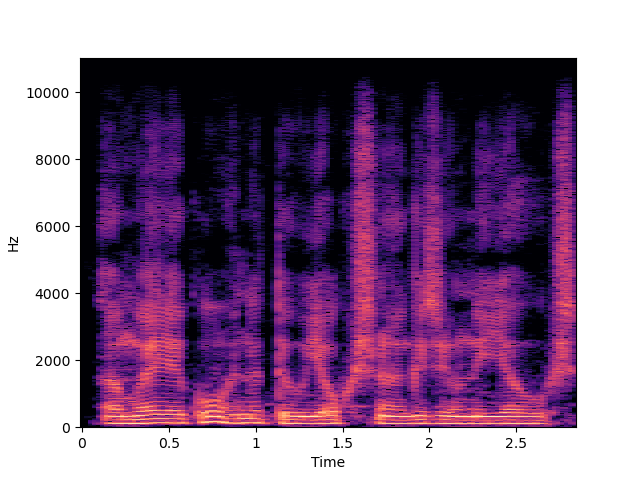
\includegraphics{figures/cherooke.png}}
    \end{center}
    \caption{Spettrogramma vocale (Cherooke dagli esempi audio di Max MSP)}
\end{figure}

Se la frequenza è rappresentata in maniera lineare, una stessa differenza frequenziale corrisponderà a una stessa distanza nel grafico: per esempio, una differenza di 1000 Hz potrebbe corrispondere a 1 cm sull'asse orizzontale. Lo stesso vale per l'ampiezza e le grandezze a essa linearmente correlate: per esempio, una differenza di 0.1 in ampiezza normalizzata, o una differenza di 0.5 V, potrebbero corrispondere a 1 cm sull'asse verticale. 

Se invece la frequenza è rappresentata in maniera logaritmica, uguali rapporti di frequenza corrisponderanno a uguali distanze nel grafico: per esempio, un rapporto frequenziale di 2:1, ovvero un intervallo d'ottava, potrebbe corrispondere a 1 cm nel grafico; questo vuol dire che una rappresentazione frequenziale logaritmica è lineare nello spazio delle altezze, per cui intervalli uguali corrisponderanno a distanze grafiche uguali. Uno spettrogramma con rappresentazione logaritmica delle frequenze è un oggetto piuttosto simile a una partitura. Se l'ampiezza è rappresentata su una scala logaritmica, questo equivale a dire che le differenze in decibel sono mostrate linearmente: per esempio, un rapporto di ampiezze di 2:1, ovvero una differenza di circa 6 dB, potrebbe corrispondere a 1 cm. 





\section{Categorie di spettri}

Possiamo suddividere gli spettri in alcune categorie differenti. 


\subsection{Spettri armonici}

Come già detto, un segnale periodico nel dominio del tempo produce uno spettro armonico. Questo vuol dire che le frequenze di tutte le sue componenti sono multiple della frequenza fondamentale, corrispondente all'inverso del periodo del segnale.

In una rappresentazione grafica nel dominio della frequenza rappresentata linearmente, tutte le sue componenti sono equidistanti sull'asse delle ascisse, e la stessa distanza c'è tra la fondamentale e l'asse delle ordinate.

Il caso più semplice di spettro armonico è quello della sinusoide, che ha una sola componente di ampiezza non nulla, alla frequenza fondamentale.

È utile conoscere le conformazioni spettrali di alcuni altri segnali periodici:

\begin{itemize}

\item L'onda a dente di sega è composta da una somma di sinusoidi armoniche con termine di fase nullo. L'ampiezza di ciascuna armonica è inversamente proporzionale al suo ordine: se la fondamentale (armonica 1) ha ampiezza 1, allora la seconda armonica (di frequenza doppia) ha ampiezza $\frac{1}{2}$, la terza armonica (di frequenza tripla rispetto alla fondamentale) ha ampiezza $\frac{1}{3}$ e così via. In termini percettivi, questo produce un suono molto brillante: la decima armonica ha ampiezza $\frac{1}{10}$, corrispondente a -20 dB, rispetto alla fondamentale; la centesima armonica ha ampiezza $\frac{1}{100}$, corrispondente a -40 dB, il che vuol dire che nelle giuste condizioni può essere ancora chiaramente percepibile.

\begin{figure}
    \begin{center}
       \scalebox{0.6} {%% Creator: Matplotlib, PGF backend
%%
%% To include the figure in your LaTeX document, write
%%   \input{<filename>.pgf}
%%
%% Make sure the required packages are loaded in your preamble
%%   \usepackage{pgf}
%%
%% Also ensure that all the required font packages are loaded; for instance,
%% the lmodern package is sometimes necessary when using math font.
%%   \usepackage{lmodern}
%%
%% Figures using additional raster images can only be included by \input if
%% they are in the same directory as the main LaTeX file. For loading figures
%% from other directories you can use the `import` package
%%   \usepackage{import}
%%
%% and then include the figures with
%%   \import{<path to file>}{<filename>.pgf}
%%
%% Matplotlib used the following preamble
%%   
%%   \makeatletter\@ifpackageloaded{underscore}{}{\usepackage[strings]{underscore}}\makeatother
%%
\begingroup%
\makeatletter%
\begin{pgfpicture}%
\pgfpathrectangle{\pgfpointorigin}{\pgfqpoint{6.400000in}{4.800000in}}%
\pgfusepath{use as bounding box, clip}%
\begin{pgfscope}%
\pgfsetbuttcap%
\pgfsetmiterjoin%
\definecolor{currentfill}{rgb}{1.000000,1.000000,1.000000}%
\pgfsetfillcolor{currentfill}%
\pgfsetlinewidth{0.000000pt}%
\definecolor{currentstroke}{rgb}{1.000000,1.000000,1.000000}%
\pgfsetstrokecolor{currentstroke}%
\pgfsetdash{}{0pt}%
\pgfpathmoveto{\pgfqpoint{0.000000in}{0.000000in}}%
\pgfpathlineto{\pgfqpoint{6.400000in}{0.000000in}}%
\pgfpathlineto{\pgfqpoint{6.400000in}{4.800000in}}%
\pgfpathlineto{\pgfqpoint{0.000000in}{4.800000in}}%
\pgfpathlineto{\pgfqpoint{0.000000in}{0.000000in}}%
\pgfpathclose%
\pgfusepath{fill}%
\end{pgfscope}%
\begin{pgfscope}%
\pgfsetbuttcap%
\pgfsetmiterjoin%
\definecolor{currentfill}{rgb}{1.000000,1.000000,1.000000}%
\pgfsetfillcolor{currentfill}%
\pgfsetlinewidth{0.000000pt}%
\definecolor{currentstroke}{rgb}{0.000000,0.000000,0.000000}%
\pgfsetstrokecolor{currentstroke}%
\pgfsetstrokeopacity{0.000000}%
\pgfsetdash{}{0pt}%
\pgfpathmoveto{\pgfqpoint{0.800000in}{0.528000in}}%
\pgfpathlineto{\pgfqpoint{5.760000in}{0.528000in}}%
\pgfpathlineto{\pgfqpoint{5.760000in}{4.224000in}}%
\pgfpathlineto{\pgfqpoint{0.800000in}{4.224000in}}%
\pgfpathlineto{\pgfqpoint{0.800000in}{0.528000in}}%
\pgfpathclose%
\pgfusepath{fill}%
\end{pgfscope}%
\begin{pgfscope}%
\pgfsetbuttcap%
\pgfsetroundjoin%
\definecolor{currentfill}{rgb}{0.000000,0.000000,0.000000}%
\pgfsetfillcolor{currentfill}%
\pgfsetlinewidth{0.803000pt}%
\definecolor{currentstroke}{rgb}{0.000000,0.000000,0.000000}%
\pgfsetstrokecolor{currentstroke}%
\pgfsetdash{}{0pt}%
\pgfsys@defobject{currentmarker}{\pgfqpoint{0.000000in}{-0.048611in}}{\pgfqpoint{0.000000in}{0.000000in}}{%
\pgfpathmoveto{\pgfqpoint{0.000000in}{0.000000in}}%
\pgfpathlineto{\pgfqpoint{0.000000in}{-0.048611in}}%
\pgfusepath{stroke,fill}%
}%
\begin{pgfscope}%
\pgfsys@transformshift{1.025455in}{0.528000in}%
\pgfsys@useobject{currentmarker}{}%
\end{pgfscope}%
\end{pgfscope}%
\begin{pgfscope}%
\definecolor{textcolor}{rgb}{0.000000,0.000000,0.000000}%
\pgfsetstrokecolor{textcolor}%
\pgfsetfillcolor{textcolor}%
\pgftext[x=1.025455in,y=0.430778in,,top]{\color{textcolor}\rmfamily\fontsize{10.000000}{12.000000}\selectfont \(\displaystyle {0}\)}%
\end{pgfscope}%
\begin{pgfscope}%
\pgfsetbuttcap%
\pgfsetroundjoin%
\definecolor{currentfill}{rgb}{0.000000,0.000000,0.000000}%
\pgfsetfillcolor{currentfill}%
\pgfsetlinewidth{0.803000pt}%
\definecolor{currentstroke}{rgb}{0.000000,0.000000,0.000000}%
\pgfsetstrokecolor{currentstroke}%
\pgfsetdash{}{0pt}%
\pgfsys@defobject{currentmarker}{\pgfqpoint{0.000000in}{-0.048611in}}{\pgfqpoint{0.000000in}{0.000000in}}{%
\pgfpathmoveto{\pgfqpoint{0.000000in}{0.000000in}}%
\pgfpathlineto{\pgfqpoint{0.000000in}{-0.048611in}}%
\pgfusepath{stroke,fill}%
}%
\begin{pgfscope}%
\pgfsys@transformshift{2.047971in}{0.528000in}%
\pgfsys@useobject{currentmarker}{}%
\end{pgfscope}%
\end{pgfscope}%
\begin{pgfscope}%
\definecolor{textcolor}{rgb}{0.000000,0.000000,0.000000}%
\pgfsetstrokecolor{textcolor}%
\pgfsetfillcolor{textcolor}%
\pgftext[x=2.047971in,y=0.430778in,,top]{\color{textcolor}\rmfamily\fontsize{10.000000}{12.000000}\selectfont \(\displaystyle {5000}\)}%
\end{pgfscope}%
\begin{pgfscope}%
\pgfsetbuttcap%
\pgfsetroundjoin%
\definecolor{currentfill}{rgb}{0.000000,0.000000,0.000000}%
\pgfsetfillcolor{currentfill}%
\pgfsetlinewidth{0.803000pt}%
\definecolor{currentstroke}{rgb}{0.000000,0.000000,0.000000}%
\pgfsetstrokecolor{currentstroke}%
\pgfsetdash{}{0pt}%
\pgfsys@defobject{currentmarker}{\pgfqpoint{0.000000in}{-0.048611in}}{\pgfqpoint{0.000000in}{0.000000in}}{%
\pgfpathmoveto{\pgfqpoint{0.000000in}{0.000000in}}%
\pgfpathlineto{\pgfqpoint{0.000000in}{-0.048611in}}%
\pgfusepath{stroke,fill}%
}%
\begin{pgfscope}%
\pgfsys@transformshift{3.070486in}{0.528000in}%
\pgfsys@useobject{currentmarker}{}%
\end{pgfscope}%
\end{pgfscope}%
\begin{pgfscope}%
\definecolor{textcolor}{rgb}{0.000000,0.000000,0.000000}%
\pgfsetstrokecolor{textcolor}%
\pgfsetfillcolor{textcolor}%
\pgftext[x=3.070486in,y=0.430778in,,top]{\color{textcolor}\rmfamily\fontsize{10.000000}{12.000000}\selectfont \(\displaystyle {10000}\)}%
\end{pgfscope}%
\begin{pgfscope}%
\pgfsetbuttcap%
\pgfsetroundjoin%
\definecolor{currentfill}{rgb}{0.000000,0.000000,0.000000}%
\pgfsetfillcolor{currentfill}%
\pgfsetlinewidth{0.803000pt}%
\definecolor{currentstroke}{rgb}{0.000000,0.000000,0.000000}%
\pgfsetstrokecolor{currentstroke}%
\pgfsetdash{}{0pt}%
\pgfsys@defobject{currentmarker}{\pgfqpoint{0.000000in}{-0.048611in}}{\pgfqpoint{0.000000in}{0.000000in}}{%
\pgfpathmoveto{\pgfqpoint{0.000000in}{0.000000in}}%
\pgfpathlineto{\pgfqpoint{0.000000in}{-0.048611in}}%
\pgfusepath{stroke,fill}%
}%
\begin{pgfscope}%
\pgfsys@transformshift{4.093002in}{0.528000in}%
\pgfsys@useobject{currentmarker}{}%
\end{pgfscope}%
\end{pgfscope}%
\begin{pgfscope}%
\definecolor{textcolor}{rgb}{0.000000,0.000000,0.000000}%
\pgfsetstrokecolor{textcolor}%
\pgfsetfillcolor{textcolor}%
\pgftext[x=4.093002in,y=0.430778in,,top]{\color{textcolor}\rmfamily\fontsize{10.000000}{12.000000}\selectfont \(\displaystyle {15000}\)}%
\end{pgfscope}%
\begin{pgfscope}%
\pgfsetbuttcap%
\pgfsetroundjoin%
\definecolor{currentfill}{rgb}{0.000000,0.000000,0.000000}%
\pgfsetfillcolor{currentfill}%
\pgfsetlinewidth{0.803000pt}%
\definecolor{currentstroke}{rgb}{0.000000,0.000000,0.000000}%
\pgfsetstrokecolor{currentstroke}%
\pgfsetdash{}{0pt}%
\pgfsys@defobject{currentmarker}{\pgfqpoint{0.000000in}{-0.048611in}}{\pgfqpoint{0.000000in}{0.000000in}}{%
\pgfpathmoveto{\pgfqpoint{0.000000in}{0.000000in}}%
\pgfpathlineto{\pgfqpoint{0.000000in}{-0.048611in}}%
\pgfusepath{stroke,fill}%
}%
\begin{pgfscope}%
\pgfsys@transformshift{5.115518in}{0.528000in}%
\pgfsys@useobject{currentmarker}{}%
\end{pgfscope}%
\end{pgfscope}%
\begin{pgfscope}%
\definecolor{textcolor}{rgb}{0.000000,0.000000,0.000000}%
\pgfsetstrokecolor{textcolor}%
\pgfsetfillcolor{textcolor}%
\pgftext[x=5.115518in,y=0.430778in,,top]{\color{textcolor}\rmfamily\fontsize{10.000000}{12.000000}\selectfont \(\displaystyle {20000}\)}%
\end{pgfscope}%
\begin{pgfscope}%
\pgfsetbuttcap%
\pgfsetroundjoin%
\definecolor{currentfill}{rgb}{0.000000,0.000000,0.000000}%
\pgfsetfillcolor{currentfill}%
\pgfsetlinewidth{0.803000pt}%
\definecolor{currentstroke}{rgb}{0.000000,0.000000,0.000000}%
\pgfsetstrokecolor{currentstroke}%
\pgfsetdash{}{0pt}%
\pgfsys@defobject{currentmarker}{\pgfqpoint{-0.048611in}{0.000000in}}{\pgfqpoint{-0.000000in}{0.000000in}}{%
\pgfpathmoveto{\pgfqpoint{-0.000000in}{0.000000in}}%
\pgfpathlineto{\pgfqpoint{-0.048611in}{0.000000in}}%
\pgfusepath{stroke,fill}%
}%
\begin{pgfscope}%
\pgfsys@transformshift{0.800000in}{0.546200in}%
\pgfsys@useobject{currentmarker}{}%
\end{pgfscope}%
\end{pgfscope}%
\begin{pgfscope}%
\definecolor{textcolor}{rgb}{0.000000,0.000000,0.000000}%
\pgfsetstrokecolor{textcolor}%
\pgfsetfillcolor{textcolor}%
\pgftext[x=0.417283in, y=0.497975in, left, base]{\color{textcolor}\rmfamily\fontsize{10.000000}{12.000000}\selectfont \(\displaystyle {\ensuremath{-}2.0}\)}%
\end{pgfscope}%
\begin{pgfscope}%
\pgfsetbuttcap%
\pgfsetroundjoin%
\definecolor{currentfill}{rgb}{0.000000,0.000000,0.000000}%
\pgfsetfillcolor{currentfill}%
\pgfsetlinewidth{0.803000pt}%
\definecolor{currentstroke}{rgb}{0.000000,0.000000,0.000000}%
\pgfsetstrokecolor{currentstroke}%
\pgfsetdash{}{0pt}%
\pgfsys@defobject{currentmarker}{\pgfqpoint{-0.048611in}{0.000000in}}{\pgfqpoint{-0.000000in}{0.000000in}}{%
\pgfpathmoveto{\pgfqpoint{-0.000000in}{0.000000in}}%
\pgfpathlineto{\pgfqpoint{-0.048611in}{0.000000in}}%
\pgfusepath{stroke,fill}%
}%
\begin{pgfscope}%
\pgfsys@transformshift{0.800000in}{1.003650in}%
\pgfsys@useobject{currentmarker}{}%
\end{pgfscope}%
\end{pgfscope}%
\begin{pgfscope}%
\definecolor{textcolor}{rgb}{0.000000,0.000000,0.000000}%
\pgfsetstrokecolor{textcolor}%
\pgfsetfillcolor{textcolor}%
\pgftext[x=0.417283in, y=0.955425in, left, base]{\color{textcolor}\rmfamily\fontsize{10.000000}{12.000000}\selectfont \(\displaystyle {\ensuremath{-}1.5}\)}%
\end{pgfscope}%
\begin{pgfscope}%
\pgfsetbuttcap%
\pgfsetroundjoin%
\definecolor{currentfill}{rgb}{0.000000,0.000000,0.000000}%
\pgfsetfillcolor{currentfill}%
\pgfsetlinewidth{0.803000pt}%
\definecolor{currentstroke}{rgb}{0.000000,0.000000,0.000000}%
\pgfsetstrokecolor{currentstroke}%
\pgfsetdash{}{0pt}%
\pgfsys@defobject{currentmarker}{\pgfqpoint{-0.048611in}{0.000000in}}{\pgfqpoint{-0.000000in}{0.000000in}}{%
\pgfpathmoveto{\pgfqpoint{-0.000000in}{0.000000in}}%
\pgfpathlineto{\pgfqpoint{-0.048611in}{0.000000in}}%
\pgfusepath{stroke,fill}%
}%
\begin{pgfscope}%
\pgfsys@transformshift{0.800000in}{1.461100in}%
\pgfsys@useobject{currentmarker}{}%
\end{pgfscope}%
\end{pgfscope}%
\begin{pgfscope}%
\definecolor{textcolor}{rgb}{0.000000,0.000000,0.000000}%
\pgfsetstrokecolor{textcolor}%
\pgfsetfillcolor{textcolor}%
\pgftext[x=0.417283in, y=1.412875in, left, base]{\color{textcolor}\rmfamily\fontsize{10.000000}{12.000000}\selectfont \(\displaystyle {\ensuremath{-}1.0}\)}%
\end{pgfscope}%
\begin{pgfscope}%
\pgfsetbuttcap%
\pgfsetroundjoin%
\definecolor{currentfill}{rgb}{0.000000,0.000000,0.000000}%
\pgfsetfillcolor{currentfill}%
\pgfsetlinewidth{0.803000pt}%
\definecolor{currentstroke}{rgb}{0.000000,0.000000,0.000000}%
\pgfsetstrokecolor{currentstroke}%
\pgfsetdash{}{0pt}%
\pgfsys@defobject{currentmarker}{\pgfqpoint{-0.048611in}{0.000000in}}{\pgfqpoint{-0.000000in}{0.000000in}}{%
\pgfpathmoveto{\pgfqpoint{-0.000000in}{0.000000in}}%
\pgfpathlineto{\pgfqpoint{-0.048611in}{0.000000in}}%
\pgfusepath{stroke,fill}%
}%
\begin{pgfscope}%
\pgfsys@transformshift{0.800000in}{1.918550in}%
\pgfsys@useobject{currentmarker}{}%
\end{pgfscope}%
\end{pgfscope}%
\begin{pgfscope}%
\definecolor{textcolor}{rgb}{0.000000,0.000000,0.000000}%
\pgfsetstrokecolor{textcolor}%
\pgfsetfillcolor{textcolor}%
\pgftext[x=0.417283in, y=1.870325in, left, base]{\color{textcolor}\rmfamily\fontsize{10.000000}{12.000000}\selectfont \(\displaystyle {\ensuremath{-}0.5}\)}%
\end{pgfscope}%
\begin{pgfscope}%
\pgfsetbuttcap%
\pgfsetroundjoin%
\definecolor{currentfill}{rgb}{0.000000,0.000000,0.000000}%
\pgfsetfillcolor{currentfill}%
\pgfsetlinewidth{0.803000pt}%
\definecolor{currentstroke}{rgb}{0.000000,0.000000,0.000000}%
\pgfsetstrokecolor{currentstroke}%
\pgfsetdash{}{0pt}%
\pgfsys@defobject{currentmarker}{\pgfqpoint{-0.048611in}{0.000000in}}{\pgfqpoint{-0.000000in}{0.000000in}}{%
\pgfpathmoveto{\pgfqpoint{-0.000000in}{0.000000in}}%
\pgfpathlineto{\pgfqpoint{-0.048611in}{0.000000in}}%
\pgfusepath{stroke,fill}%
}%
\begin{pgfscope}%
\pgfsys@transformshift{0.800000in}{2.376000in}%
\pgfsys@useobject{currentmarker}{}%
\end{pgfscope}%
\end{pgfscope}%
\begin{pgfscope}%
\definecolor{textcolor}{rgb}{0.000000,0.000000,0.000000}%
\pgfsetstrokecolor{textcolor}%
\pgfsetfillcolor{textcolor}%
\pgftext[x=0.525308in, y=2.327775in, left, base]{\color{textcolor}\rmfamily\fontsize{10.000000}{12.000000}\selectfont \(\displaystyle {0.0}\)}%
\end{pgfscope}%
\begin{pgfscope}%
\pgfsetbuttcap%
\pgfsetroundjoin%
\definecolor{currentfill}{rgb}{0.000000,0.000000,0.000000}%
\pgfsetfillcolor{currentfill}%
\pgfsetlinewidth{0.803000pt}%
\definecolor{currentstroke}{rgb}{0.000000,0.000000,0.000000}%
\pgfsetstrokecolor{currentstroke}%
\pgfsetdash{}{0pt}%
\pgfsys@defobject{currentmarker}{\pgfqpoint{-0.048611in}{0.000000in}}{\pgfqpoint{-0.000000in}{0.000000in}}{%
\pgfpathmoveto{\pgfqpoint{-0.000000in}{0.000000in}}%
\pgfpathlineto{\pgfqpoint{-0.048611in}{0.000000in}}%
\pgfusepath{stroke,fill}%
}%
\begin{pgfscope}%
\pgfsys@transformshift{0.800000in}{2.833450in}%
\pgfsys@useobject{currentmarker}{}%
\end{pgfscope}%
\end{pgfscope}%
\begin{pgfscope}%
\definecolor{textcolor}{rgb}{0.000000,0.000000,0.000000}%
\pgfsetstrokecolor{textcolor}%
\pgfsetfillcolor{textcolor}%
\pgftext[x=0.525308in, y=2.785225in, left, base]{\color{textcolor}\rmfamily\fontsize{10.000000}{12.000000}\selectfont \(\displaystyle {0.5}\)}%
\end{pgfscope}%
\begin{pgfscope}%
\pgfsetbuttcap%
\pgfsetroundjoin%
\definecolor{currentfill}{rgb}{0.000000,0.000000,0.000000}%
\pgfsetfillcolor{currentfill}%
\pgfsetlinewidth{0.803000pt}%
\definecolor{currentstroke}{rgb}{0.000000,0.000000,0.000000}%
\pgfsetstrokecolor{currentstroke}%
\pgfsetdash{}{0pt}%
\pgfsys@defobject{currentmarker}{\pgfqpoint{-0.048611in}{0.000000in}}{\pgfqpoint{-0.000000in}{0.000000in}}{%
\pgfpathmoveto{\pgfqpoint{-0.000000in}{0.000000in}}%
\pgfpathlineto{\pgfqpoint{-0.048611in}{0.000000in}}%
\pgfusepath{stroke,fill}%
}%
\begin{pgfscope}%
\pgfsys@transformshift{0.800000in}{3.290900in}%
\pgfsys@useobject{currentmarker}{}%
\end{pgfscope}%
\end{pgfscope}%
\begin{pgfscope}%
\definecolor{textcolor}{rgb}{0.000000,0.000000,0.000000}%
\pgfsetstrokecolor{textcolor}%
\pgfsetfillcolor{textcolor}%
\pgftext[x=0.525308in, y=3.242675in, left, base]{\color{textcolor}\rmfamily\fontsize{10.000000}{12.000000}\selectfont \(\displaystyle {1.0}\)}%
\end{pgfscope}%
\begin{pgfscope}%
\pgfsetbuttcap%
\pgfsetroundjoin%
\definecolor{currentfill}{rgb}{0.000000,0.000000,0.000000}%
\pgfsetfillcolor{currentfill}%
\pgfsetlinewidth{0.803000pt}%
\definecolor{currentstroke}{rgb}{0.000000,0.000000,0.000000}%
\pgfsetstrokecolor{currentstroke}%
\pgfsetdash{}{0pt}%
\pgfsys@defobject{currentmarker}{\pgfqpoint{-0.048611in}{0.000000in}}{\pgfqpoint{-0.000000in}{0.000000in}}{%
\pgfpathmoveto{\pgfqpoint{-0.000000in}{0.000000in}}%
\pgfpathlineto{\pgfqpoint{-0.048611in}{0.000000in}}%
\pgfusepath{stroke,fill}%
}%
\begin{pgfscope}%
\pgfsys@transformshift{0.800000in}{3.748350in}%
\pgfsys@useobject{currentmarker}{}%
\end{pgfscope}%
\end{pgfscope}%
\begin{pgfscope}%
\definecolor{textcolor}{rgb}{0.000000,0.000000,0.000000}%
\pgfsetstrokecolor{textcolor}%
\pgfsetfillcolor{textcolor}%
\pgftext[x=0.525308in, y=3.700125in, left, base]{\color{textcolor}\rmfamily\fontsize{10.000000}{12.000000}\selectfont \(\displaystyle {1.5}\)}%
\end{pgfscope}%
\begin{pgfscope}%
\pgfsetbuttcap%
\pgfsetroundjoin%
\definecolor{currentfill}{rgb}{0.000000,0.000000,0.000000}%
\pgfsetfillcolor{currentfill}%
\pgfsetlinewidth{0.803000pt}%
\definecolor{currentstroke}{rgb}{0.000000,0.000000,0.000000}%
\pgfsetstrokecolor{currentstroke}%
\pgfsetdash{}{0pt}%
\pgfsys@defobject{currentmarker}{\pgfqpoint{-0.048611in}{0.000000in}}{\pgfqpoint{-0.000000in}{0.000000in}}{%
\pgfpathmoveto{\pgfqpoint{-0.000000in}{0.000000in}}%
\pgfpathlineto{\pgfqpoint{-0.048611in}{0.000000in}}%
\pgfusepath{stroke,fill}%
}%
\begin{pgfscope}%
\pgfsys@transformshift{0.800000in}{4.205800in}%
\pgfsys@useobject{currentmarker}{}%
\end{pgfscope}%
\end{pgfscope}%
\begin{pgfscope}%
\definecolor{textcolor}{rgb}{0.000000,0.000000,0.000000}%
\pgfsetstrokecolor{textcolor}%
\pgfsetfillcolor{textcolor}%
\pgftext[x=0.525308in, y=4.157575in, left, base]{\color{textcolor}\rmfamily\fontsize{10.000000}{12.000000}\selectfont \(\displaystyle {2.0}\)}%
\end{pgfscope}%
\begin{pgfscope}%
\pgfpathrectangle{\pgfqpoint{0.800000in}{0.528000in}}{\pgfqpoint{4.960000in}{3.696000in}}%
\pgfusepath{clip}%
\pgfsetrectcap%
\pgfsetroundjoin%
\pgfsetlinewidth{1.505625pt}%
\definecolor{currentstroke}{rgb}{0.121569,0.466667,0.705882}%
\pgfsetstrokecolor{currentstroke}%
\pgfsetdash{}{0pt}%
\pgfpathmoveto{\pgfqpoint{1.025455in}{2.376000in}}%
\pgfpathlineto{\pgfqpoint{1.031999in}{3.761365in}}%
\pgfpathlineto{\pgfqpoint{1.035066in}{4.026061in}}%
\pgfpathlineto{\pgfqpoint{1.036702in}{4.056000in}}%
\pgfpathlineto{\pgfqpoint{1.036907in}{4.055128in}}%
\pgfpathlineto{\pgfqpoint{1.037929in}{4.037800in}}%
\pgfpathlineto{\pgfqpoint{1.040179in}{3.943639in}}%
\pgfpathlineto{\pgfqpoint{1.046518in}{3.657639in}}%
\pgfpathlineto{\pgfqpoint{1.047950in}{3.644787in}}%
\pgfpathlineto{\pgfqpoint{1.048359in}{3.645488in}}%
\pgfpathlineto{\pgfqpoint{1.049381in}{3.654953in}}%
\pgfpathlineto{\pgfqpoint{1.051631in}{3.705914in}}%
\pgfpathlineto{\pgfqpoint{1.057971in}{3.861843in}}%
\pgfpathlineto{\pgfqpoint{1.058993in}{3.865471in}}%
\pgfpathlineto{\pgfqpoint{1.059402in}{3.864667in}}%
\pgfpathlineto{\pgfqpoint{1.060629in}{3.854985in}}%
\pgfpathlineto{\pgfqpoint{1.063083in}{3.809886in}}%
\pgfpathlineto{\pgfqpoint{1.069423in}{3.687416in}}%
\pgfpathlineto{\pgfqpoint{1.070650in}{3.683819in}}%
\pgfpathlineto{\pgfqpoint{1.070854in}{3.684053in}}%
\pgfpathlineto{\pgfqpoint{1.071877in}{3.688588in}}%
\pgfpathlineto{\pgfqpoint{1.073922in}{3.711636in}}%
\pgfpathlineto{\pgfqpoint{1.080875in}{3.799306in}}%
\pgfpathlineto{\pgfqpoint{1.081488in}{3.799535in}}%
\pgfpathlineto{\pgfqpoint{1.081693in}{3.799228in}}%
\pgfpathlineto{\pgfqpoint{1.082920in}{3.793487in}}%
\pgfpathlineto{\pgfqpoint{1.085169in}{3.768351in}}%
\pgfpathlineto{\pgfqpoint{1.092327in}{3.679883in}}%
\pgfpathlineto{\pgfqpoint{1.093145in}{3.678771in}}%
\pgfpathlineto{\pgfqpoint{1.093554in}{3.679160in}}%
\pgfpathlineto{\pgfqpoint{1.094781in}{3.683853in}}%
\pgfpathlineto{\pgfqpoint{1.097235in}{3.705369in}}%
\pgfpathlineto{\pgfqpoint{1.102757in}{3.753668in}}%
\pgfpathlineto{\pgfqpoint{1.103779in}{3.754728in}}%
\pgfpathlineto{\pgfqpoint{1.103984in}{3.754530in}}%
\pgfpathlineto{\pgfqpoint{1.105211in}{3.750518in}}%
\pgfpathlineto{\pgfqpoint{1.107460in}{3.732277in}}%
\pgfpathlineto{\pgfqpoint{1.115027in}{3.662588in}}%
\pgfpathlineto{\pgfqpoint{1.115845in}{3.662113in}}%
\pgfpathlineto{\pgfqpoint{1.116254in}{3.662576in}}%
\pgfpathlineto{\pgfqpoint{1.117685in}{3.667553in}}%
\pgfpathlineto{\pgfqpoint{1.120753in}{3.689910in}}%
\pgfpathlineto{\pgfqpoint{1.124843in}{3.715702in}}%
\pgfpathlineto{\pgfqpoint{1.126070in}{3.717095in}}%
\pgfpathlineto{\pgfqpoint{1.126275in}{3.716958in}}%
\pgfpathlineto{\pgfqpoint{1.127502in}{3.713919in}}%
\pgfpathlineto{\pgfqpoint{1.129751in}{3.699613in}}%
\pgfpathlineto{\pgfqpoint{1.137727in}{3.640825in}}%
\pgfpathlineto{\pgfqpoint{1.138749in}{3.640935in}}%
\pgfpathlineto{\pgfqpoint{1.138954in}{3.641232in}}%
\pgfpathlineto{\pgfqpoint{1.140590in}{3.646511in}}%
\pgfpathlineto{\pgfqpoint{1.144680in}{3.671206in}}%
\pgfpathlineto{\pgfqpoint{1.147747in}{3.682533in}}%
\pgfpathlineto{\pgfqpoint{1.148770in}{3.682474in}}%
\pgfpathlineto{\pgfqpoint{1.148974in}{3.682201in}}%
\pgfpathlineto{\pgfqpoint{1.150406in}{3.677907in}}%
\pgfpathlineto{\pgfqpoint{1.153065in}{3.660834in}}%
\pgfpathlineto{\pgfqpoint{1.159404in}{3.618397in}}%
\pgfpathlineto{\pgfqpoint{1.161040in}{3.616808in}}%
\pgfpathlineto{\pgfqpoint{1.162267in}{3.618802in}}%
\pgfpathlineto{\pgfqpoint{1.164721in}{3.628825in}}%
\pgfpathlineto{\pgfqpoint{1.169834in}{3.649765in}}%
\pgfpathlineto{\pgfqpoint{1.171061in}{3.649990in}}%
\pgfpathlineto{\pgfqpoint{1.171265in}{3.649771in}}%
\pgfpathlineto{\pgfqpoint{1.172697in}{3.646198in}}%
\pgfpathlineto{\pgfqpoint{1.175355in}{3.631609in}}%
\pgfpathlineto{\pgfqpoint{1.182104in}{3.592602in}}%
\pgfpathlineto{\pgfqpoint{1.183740in}{3.591647in}}%
\pgfpathlineto{\pgfqpoint{1.185172in}{3.594127in}}%
\pgfpathlineto{\pgfqpoint{1.188035in}{3.605038in}}%
\pgfpathlineto{\pgfqpoint{1.192125in}{3.618310in}}%
\pgfpathlineto{\pgfqpoint{1.193556in}{3.618382in}}%
\pgfpathlineto{\pgfqpoint{1.194988in}{3.615344in}}%
\pgfpathlineto{\pgfqpoint{1.197442in}{3.603831in}}%
\pgfpathlineto{\pgfqpoint{1.204804in}{3.566119in}}%
\pgfpathlineto{\pgfqpoint{1.206440in}{3.565635in}}%
\pgfpathlineto{\pgfqpoint{1.208076in}{3.568555in}}%
\pgfpathlineto{\pgfqpoint{1.215438in}{3.587911in}}%
\pgfpathlineto{\pgfqpoint{1.216052in}{3.587463in}}%
\pgfpathlineto{\pgfqpoint{1.217688in}{3.583801in}}%
\pgfpathlineto{\pgfqpoint{1.220551in}{3.570302in}}%
\pgfpathlineto{\pgfqpoint{1.226890in}{3.540090in}}%
\pgfpathlineto{\pgfqpoint{1.228731in}{3.538782in}}%
\pgfpathlineto{\pgfqpoint{1.230367in}{3.540928in}}%
\pgfpathlineto{\pgfqpoint{1.233843in}{3.551049in}}%
\pgfpathlineto{\pgfqpoint{1.237115in}{3.557544in}}%
\pgfpathlineto{\pgfqpoint{1.238547in}{3.557016in}}%
\pgfpathlineto{\pgfqpoint{1.240387in}{3.552731in}}%
\pgfpathlineto{\pgfqpoint{1.243659in}{3.537436in}}%
\pgfpathlineto{\pgfqpoint{1.248977in}{3.513771in}}%
\pgfpathlineto{\pgfqpoint{1.251022in}{3.511632in}}%
\pgfpathlineto{\pgfqpoint{1.252453in}{3.512827in}}%
\pgfpathlineto{\pgfqpoint{1.255112in}{3.518945in}}%
\pgfpathlineto{\pgfqpoint{1.259406in}{3.527577in}}%
\pgfpathlineto{\pgfqpoint{1.260838in}{3.527149in}}%
\pgfpathlineto{\pgfqpoint{1.262678in}{3.523322in}}%
\pgfpathlineto{\pgfqpoint{1.265746in}{3.510357in}}%
\pgfpathlineto{\pgfqpoint{1.271676in}{3.485903in}}%
\pgfpathlineto{\pgfqpoint{1.273721in}{3.484286in}}%
\pgfpathlineto{\pgfqpoint{1.275357in}{3.485860in}}%
\pgfpathlineto{\pgfqpoint{1.279243in}{3.494456in}}%
\pgfpathlineto{\pgfqpoint{1.282106in}{3.497967in}}%
\pgfpathlineto{\pgfqpoint{1.283538in}{3.497045in}}%
\pgfpathlineto{\pgfqpoint{1.285583in}{3.492212in}}%
\pgfpathlineto{\pgfqpoint{1.289468in}{3.475266in}}%
\pgfpathlineto{\pgfqpoint{1.293967in}{3.458638in}}%
\pgfpathlineto{\pgfqpoint{1.296217in}{3.456681in}}%
\pgfpathlineto{\pgfqpoint{1.297853in}{3.458041in}}%
\pgfpathlineto{\pgfqpoint{1.301943in}{3.465973in}}%
\pgfpathlineto{\pgfqpoint{1.304601in}{3.468446in}}%
\pgfpathlineto{\pgfqpoint{1.306237in}{3.467066in}}%
\pgfpathlineto{\pgfqpoint{1.308487in}{3.461235in}}%
\pgfpathlineto{\pgfqpoint{1.318712in}{3.428912in}}%
\pgfpathlineto{\pgfqpoint{1.320553in}{3.430356in}}%
\pgfpathlineto{\pgfqpoint{1.327710in}{3.438753in}}%
\pgfpathlineto{\pgfqpoint{1.329551in}{3.435913in}}%
\pgfpathlineto{\pgfqpoint{1.332414in}{3.426426in}}%
\pgfpathlineto{\pgfqpoint{1.339367in}{3.402218in}}%
\pgfpathlineto{\pgfqpoint{1.341412in}{3.401044in}}%
\pgfpathlineto{\pgfqpoint{1.343457in}{3.402802in}}%
\pgfpathlineto{\pgfqpoint{1.349592in}{3.409756in}}%
\pgfpathlineto{\pgfqpoint{1.351228in}{3.408123in}}%
\pgfpathlineto{\pgfqpoint{1.353682in}{3.401796in}}%
\pgfpathlineto{\pgfqpoint{1.363089in}{3.373123in}}%
\pgfpathlineto{\pgfqpoint{1.364930in}{3.373537in}}%
\pgfpathlineto{\pgfqpoint{1.367997in}{3.377512in}}%
\pgfpathlineto{\pgfqpoint{1.371474in}{3.380678in}}%
\pgfpathlineto{\pgfqpoint{1.373314in}{3.379431in}}%
\pgfpathlineto{\pgfqpoint{1.375564in}{3.374490in}}%
\pgfpathlineto{\pgfqpoint{1.380472in}{3.356282in}}%
\pgfpathlineto{\pgfqpoint{1.384358in}{3.346100in}}%
\pgfpathlineto{\pgfqpoint{1.386607in}{3.344976in}}%
\pgfpathlineto{\pgfqpoint{1.388857in}{3.346790in}}%
\pgfpathlineto{\pgfqpoint{1.393969in}{3.351591in}}%
\pgfpathlineto{\pgfqpoint{1.395810in}{3.350204in}}%
\pgfpathlineto{\pgfqpoint{1.398264in}{3.344683in}}%
\pgfpathlineto{\pgfqpoint{1.408489in}{3.316787in}}%
\pgfpathlineto{\pgfqpoint{1.410534in}{3.317612in}}%
\pgfpathlineto{\pgfqpoint{1.417078in}{3.322300in}}%
\pgfpathlineto{\pgfqpoint{1.419123in}{3.319631in}}%
\pgfpathlineto{\pgfqpoint{1.422191in}{3.310898in}}%
\pgfpathlineto{\pgfqpoint{1.429348in}{3.289705in}}%
\pgfpathlineto{\pgfqpoint{1.431598in}{3.288577in}}%
\pgfpathlineto{\pgfqpoint{1.434052in}{3.290233in}}%
\pgfpathlineto{\pgfqpoint{1.438755in}{3.293604in}}%
\pgfpathlineto{\pgfqpoint{1.440596in}{3.292218in}}%
\pgfpathlineto{\pgfqpoint{1.443050in}{3.287049in}}%
\pgfpathlineto{\pgfqpoint{1.453480in}{3.260320in}}%
\pgfpathlineto{\pgfqpoint{1.455729in}{3.261086in}}%
\pgfpathlineto{\pgfqpoint{1.461660in}{3.264500in}}%
\pgfpathlineto{\pgfqpoint{1.463705in}{3.262197in}}%
\pgfpathlineto{\pgfqpoint{1.466568in}{3.254960in}}%
\pgfpathlineto{\pgfqpoint{1.474544in}{3.232892in}}%
\pgfpathlineto{\pgfqpoint{1.476793in}{3.232017in}}%
\pgfpathlineto{\pgfqpoint{1.479452in}{3.233670in}}%
\pgfpathlineto{\pgfqpoint{1.483542in}{3.235795in}}%
\pgfpathlineto{\pgfqpoint{1.485587in}{3.234138in}}%
\pgfpathlineto{\pgfqpoint{1.488245in}{3.228416in}}%
\pgfpathlineto{\pgfqpoint{1.497857in}{3.203917in}}%
\pgfpathlineto{\pgfqpoint{1.500106in}{3.203920in}}%
\pgfpathlineto{\pgfqpoint{1.507060in}{3.206324in}}%
\pgfpathlineto{\pgfqpoint{1.509309in}{3.202961in}}%
\pgfpathlineto{\pgfqpoint{1.512990in}{3.192483in}}%
\pgfpathlineto{\pgfqpoint{1.518716in}{3.177162in}}%
\pgfpathlineto{\pgfqpoint{1.521375in}{3.175261in}}%
\pgfpathlineto{\pgfqpoint{1.524033in}{3.176329in}}%
\pgfpathlineto{\pgfqpoint{1.528328in}{3.178118in}}%
\pgfpathlineto{\pgfqpoint{1.530373in}{3.176479in}}%
\pgfpathlineto{\pgfqpoint{1.533031in}{3.171039in}}%
\pgfpathlineto{\pgfqpoint{1.543052in}{3.147062in}}%
\pgfpathlineto{\pgfqpoint{1.545506in}{3.147240in}}%
\pgfpathlineto{\pgfqpoint{1.551437in}{3.148990in}}%
\pgfpathlineto{\pgfqpoint{1.553686in}{3.146240in}}%
\pgfpathlineto{\pgfqpoint{1.556958in}{3.138012in}}%
\pgfpathlineto{\pgfqpoint{1.563911in}{3.120017in}}%
\pgfpathlineto{\pgfqpoint{1.566570in}{3.118432in}}%
\pgfpathlineto{\pgfqpoint{1.569638in}{3.119638in}}%
\pgfpathlineto{\pgfqpoint{1.573114in}{3.120540in}}%
\pgfpathlineto{\pgfqpoint{1.575364in}{3.118641in}}%
\pgfpathlineto{\pgfqpoint{1.578227in}{3.112648in}}%
\pgfpathlineto{\pgfqpoint{1.587429in}{3.090563in}}%
\pgfpathlineto{\pgfqpoint{1.589883in}{3.090083in}}%
\pgfpathlineto{\pgfqpoint{1.596836in}{3.090962in}}%
\pgfpathlineto{\pgfqpoint{1.599291in}{3.087196in}}%
\pgfpathlineto{\pgfqpoint{1.603585in}{3.075358in}}%
\pgfpathlineto{\pgfqpoint{1.608698in}{3.063332in}}%
\pgfpathlineto{\pgfqpoint{1.611561in}{3.061525in}}%
\pgfpathlineto{\pgfqpoint{1.614833in}{3.062578in}}%
\pgfpathlineto{\pgfqpoint{1.618105in}{3.062964in}}%
\pgfpathlineto{\pgfqpoint{1.620354in}{3.060879in}}%
\pgfpathlineto{\pgfqpoint{1.623422in}{3.054335in}}%
\pgfpathlineto{\pgfqpoint{1.632011in}{3.033952in}}%
\pgfpathlineto{\pgfqpoint{1.634670in}{3.033075in}}%
\pgfpathlineto{\pgfqpoint{1.641827in}{3.033296in}}%
\pgfpathlineto{\pgfqpoint{1.644486in}{3.028987in}}%
\pgfpathlineto{\pgfqpoint{1.649803in}{3.014348in}}%
\pgfpathlineto{\pgfqpoint{1.654097in}{3.005848in}}%
\pgfpathlineto{\pgfqpoint{1.656756in}{3.004550in}}%
\pgfpathlineto{\pgfqpoint{1.664936in}{3.003756in}}%
\pgfpathlineto{\pgfqpoint{1.668004in}{2.997692in}}%
\pgfpathlineto{\pgfqpoint{1.677206in}{2.976783in}}%
\pgfpathlineto{\pgfqpoint{1.679865in}{2.976084in}}%
\pgfpathlineto{\pgfqpoint{1.686409in}{2.976079in}}%
\pgfpathlineto{\pgfqpoint{1.689067in}{2.972144in}}%
\pgfpathlineto{\pgfqpoint{1.693566in}{2.960336in}}%
\pgfpathlineto{\pgfqpoint{1.698475in}{2.949505in}}%
\pgfpathlineto{\pgfqpoint{1.701338in}{2.947561in}}%
\pgfpathlineto{\pgfqpoint{1.705019in}{2.948227in}}%
\pgfpathlineto{\pgfqpoint{1.708086in}{2.947917in}}%
\pgfpathlineto{\pgfqpoint{1.710540in}{2.945197in}}%
\pgfpathlineto{\pgfqpoint{1.714017in}{2.937324in}}%
\pgfpathlineto{\pgfqpoint{1.721174in}{2.920705in}}%
\pgfpathlineto{\pgfqpoint{1.724037in}{2.919014in}}%
\pgfpathlineto{\pgfqpoint{1.732218in}{2.917596in}}%
\pgfpathlineto{\pgfqpoint{1.735285in}{2.911699in}}%
\pgfpathlineto{\pgfqpoint{1.744692in}{2.891200in}}%
\pgfpathlineto{\pgfqpoint{1.747555in}{2.890499in}}%
\pgfpathlineto{\pgfqpoint{1.753281in}{2.890292in}}%
\pgfpathlineto{\pgfqpoint{1.755940in}{2.886858in}}%
\pgfpathlineto{\pgfqpoint{1.760030in}{2.876916in}}%
\pgfpathlineto{\pgfqpoint{1.765756in}{2.864075in}}%
\pgfpathlineto{\pgfqpoint{1.768824in}{2.861967in}}%
\pgfpathlineto{\pgfqpoint{1.777413in}{2.859740in}}%
\pgfpathlineto{\pgfqpoint{1.780685in}{2.853054in}}%
\pgfpathlineto{\pgfqpoint{1.789069in}{2.834596in}}%
\pgfpathlineto{\pgfqpoint{1.791933in}{2.833365in}}%
\pgfpathlineto{\pgfqpoint{1.798681in}{2.832455in}}%
\pgfpathlineto{\pgfqpoint{1.801544in}{2.828049in}}%
\pgfpathlineto{\pgfqpoint{1.807475in}{2.812978in}}%
\pgfpathlineto{\pgfqpoint{1.811565in}{2.806024in}}%
\pgfpathlineto{\pgfqpoint{1.814632in}{2.804806in}}%
\pgfpathlineto{\pgfqpoint{1.820972in}{2.803911in}}%
\pgfpathlineto{\pgfqpoint{1.823835in}{2.799674in}}%
\pgfpathlineto{\pgfqpoint{1.829152in}{2.786291in}}%
\pgfpathlineto{\pgfqpoint{1.833651in}{2.777845in}}%
\pgfpathlineto{\pgfqpoint{1.836719in}{2.776257in}}%
\pgfpathlineto{\pgfqpoint{1.843876in}{2.774762in}}%
\pgfpathlineto{\pgfqpoint{1.846944in}{2.769584in}}%
\pgfpathlineto{\pgfqpoint{1.857578in}{2.748152in}}%
\pgfpathlineto{\pgfqpoint{1.860850in}{2.747751in}}%
\pgfpathlineto{\pgfqpoint{1.865145in}{2.747131in}}%
\pgfpathlineto{\pgfqpoint{1.867803in}{2.744011in}}%
\pgfpathlineto{\pgfqpoint{1.871689in}{2.735252in}}%
\pgfpathlineto{\pgfqpoint{1.878233in}{2.721100in}}%
\pgfpathlineto{\pgfqpoint{1.881300in}{2.719170in}}%
\pgfpathlineto{\pgfqpoint{1.889072in}{2.717051in}}%
\pgfpathlineto{\pgfqpoint{1.892344in}{2.711086in}}%
\pgfpathlineto{\pgfqpoint{1.901751in}{2.691510in}}%
\pgfpathlineto{\pgfqpoint{1.904818in}{2.690520in}}%
\pgfpathlineto{\pgfqpoint{1.910340in}{2.689582in}}%
\pgfpathlineto{\pgfqpoint{1.913203in}{2.685762in}}%
\pgfpathlineto{\pgfqpoint{1.917906in}{2.674504in}}%
\pgfpathlineto{\pgfqpoint{1.923019in}{2.664110in}}%
\pgfpathlineto{\pgfqpoint{1.926087in}{2.662055in}}%
\pgfpathlineto{\pgfqpoint{1.934062in}{2.659593in}}%
\pgfpathlineto{\pgfqpoint{1.937334in}{2.653537in}}%
\pgfpathlineto{\pgfqpoint{1.946537in}{2.634469in}}%
\pgfpathlineto{\pgfqpoint{1.949604in}{2.633357in}}%
\pgfpathlineto{\pgfqpoint{1.955331in}{2.632193in}}%
\pgfpathlineto{\pgfqpoint{1.958194in}{2.628251in}}%
\pgfpathlineto{\pgfqpoint{1.963102in}{2.616485in}}%
\pgfpathlineto{\pgfqpoint{1.968010in}{2.606856in}}%
\pgfpathlineto{\pgfqpoint{1.971282in}{2.604846in}}%
\pgfpathlineto{\pgfqpoint{1.978644in}{2.602663in}}%
\pgfpathlineto{\pgfqpoint{1.981711in}{2.597399in}}%
\pgfpathlineto{\pgfqpoint{1.992141in}{2.576832in}}%
\pgfpathlineto{\pgfqpoint{1.995618in}{2.576187in}}%
\pgfpathlineto{\pgfqpoint{1.999708in}{2.575308in}}%
\pgfpathlineto{\pgfqpoint{2.002571in}{2.571870in}}%
\pgfpathlineto{\pgfqpoint{2.006865in}{2.562133in}}%
\pgfpathlineto{\pgfqpoint{2.012796in}{2.549821in}}%
\pgfpathlineto{\pgfqpoint{2.016068in}{2.547699in}}%
\pgfpathlineto{\pgfqpoint{2.023635in}{2.545256in}}%
\pgfpathlineto{\pgfqpoint{2.026907in}{2.539427in}}%
\pgfpathlineto{\pgfqpoint{2.036518in}{2.520007in}}%
\pgfpathlineto{\pgfqpoint{2.039790in}{2.518990in}}%
\pgfpathlineto{\pgfqpoint{2.044698in}{2.517974in}}%
\pgfpathlineto{\pgfqpoint{2.047562in}{2.514410in}}%
\pgfpathlineto{\pgfqpoint{2.051856in}{2.504619in}}%
\pgfpathlineto{\pgfqpoint{2.057582in}{2.492769in}}%
\pgfpathlineto{\pgfqpoint{2.060854in}{2.490545in}}%
\pgfpathlineto{\pgfqpoint{2.068625in}{2.487862in}}%
\pgfpathlineto{\pgfqpoint{2.071897in}{2.481923in}}%
\pgfpathlineto{\pgfqpoint{2.081305in}{2.462906in}}%
\pgfpathlineto{\pgfqpoint{2.084577in}{2.461803in}}%
\pgfpathlineto{\pgfqpoint{2.089689in}{2.460651in}}%
\pgfpathlineto{\pgfqpoint{2.092552in}{2.456965in}}%
\pgfpathlineto{\pgfqpoint{2.097051in}{2.446585in}}%
\pgfpathlineto{\pgfqpoint{2.102573in}{2.435453in}}%
\pgfpathlineto{\pgfqpoint{2.105845in}{2.433337in}}%
\pgfpathlineto{\pgfqpoint{2.113207in}{2.430987in}}%
\pgfpathlineto{\pgfqpoint{2.116479in}{2.425354in}}%
\pgfpathlineto{\pgfqpoint{2.126500in}{2.405490in}}%
\pgfpathlineto{\pgfqpoint{2.129772in}{2.404601in}}%
\pgfpathlineto{\pgfqpoint{2.134475in}{2.403502in}}%
\pgfpathlineto{\pgfqpoint{2.137338in}{2.399897in}}%
\pgfpathlineto{\pgfqpoint{2.141837in}{2.389596in}}%
\pgfpathlineto{\pgfqpoint{2.147359in}{2.378363in}}%
\pgfpathlineto{\pgfqpoint{2.150631in}{2.376162in}}%
\pgfpathlineto{\pgfqpoint{2.158198in}{2.373637in}}%
\pgfpathlineto{\pgfqpoint{2.161470in}{2.367878in}}%
\pgfpathlineto{\pgfqpoint{2.171286in}{2.348349in}}%
\pgfpathlineto{\pgfqpoint{2.174558in}{2.347406in}}%
\pgfpathlineto{\pgfqpoint{2.179262in}{2.346366in}}%
\pgfpathlineto{\pgfqpoint{2.182125in}{2.342844in}}%
\pgfpathlineto{\pgfqpoint{2.186419in}{2.333127in}}%
\pgfpathlineto{\pgfqpoint{2.192350in}{2.321013in}}%
\pgfpathlineto{\pgfqpoint{2.195622in}{2.318934in}}%
\pgfpathlineto{\pgfqpoint{2.202984in}{2.316547in}}%
\pgfpathlineto{\pgfqpoint{2.206256in}{2.310870in}}%
\pgfpathlineto{\pgfqpoint{2.216072in}{2.291195in}}%
\pgfpathlineto{\pgfqpoint{2.219344in}{2.290206in}}%
\pgfpathlineto{\pgfqpoint{2.224252in}{2.289094in}}%
\pgfpathlineto{\pgfqpoint{2.227115in}{2.285450in}}%
\pgfpathlineto{\pgfqpoint{2.231614in}{2.275092in}}%
\pgfpathlineto{\pgfqpoint{2.237136in}{2.263887in}}%
\pgfpathlineto{\pgfqpoint{2.240408in}{2.261739in}}%
\pgfpathlineto{\pgfqpoint{2.247975in}{2.259231in}}%
\pgfpathlineto{\pgfqpoint{2.251247in}{2.253416in}}%
\pgfpathlineto{\pgfqpoint{2.260858in}{2.234026in}}%
\pgfpathlineto{\pgfqpoint{2.264130in}{2.233003in}}%
\pgfpathlineto{\pgfqpoint{2.269038in}{2.231993in}}%
\pgfpathlineto{\pgfqpoint{2.271902in}{2.228432in}}%
\pgfpathlineto{\pgfqpoint{2.276196in}{2.218625in}}%
\pgfpathlineto{\pgfqpoint{2.281922in}{2.206744in}}%
\pgfpathlineto{\pgfqpoint{2.285194in}{2.204534in}}%
\pgfpathlineto{\pgfqpoint{2.292965in}{2.201928in}}%
\pgfpathlineto{\pgfqpoint{2.296237in}{2.195969in}}%
\pgfpathlineto{\pgfqpoint{2.305645in}{2.176841in}}%
\pgfpathlineto{\pgfqpoint{2.308917in}{2.175794in}}%
\pgfpathlineto{\pgfqpoint{2.314029in}{2.174754in}}%
\pgfpathlineto{\pgfqpoint{2.316892in}{2.171070in}}%
\pgfpathlineto{\pgfqpoint{2.321391in}{2.160580in}}%
\pgfpathlineto{\pgfqpoint{2.326913in}{2.149337in}}%
\pgfpathlineto{\pgfqpoint{2.330185in}{2.147276in}}%
\pgfpathlineto{\pgfqpoint{2.337547in}{2.145144in}}%
\pgfpathlineto{\pgfqpoint{2.340615in}{2.139920in}}%
\pgfpathlineto{\pgfqpoint{2.351044in}{2.119221in}}%
\pgfpathlineto{\pgfqpoint{2.354316in}{2.118593in}}%
\pgfpathlineto{\pgfqpoint{2.358611in}{2.117833in}}%
\pgfpathlineto{\pgfqpoint{2.361269in}{2.114787in}}%
\pgfpathlineto{\pgfqpoint{2.365155in}{2.106245in}}%
\pgfpathlineto{\pgfqpoint{2.371699in}{2.092153in}}%
\pgfpathlineto{\pgfqpoint{2.374767in}{2.090086in}}%
\pgfpathlineto{\pgfqpoint{2.382947in}{2.087366in}}%
\pgfpathlineto{\pgfqpoint{2.386219in}{2.081089in}}%
\pgfpathlineto{\pgfqpoint{2.395012in}{2.062590in}}%
\pgfpathlineto{\pgfqpoint{2.398080in}{2.061355in}}%
\pgfpathlineto{\pgfqpoint{2.404215in}{2.060144in}}%
\pgfpathlineto{\pgfqpoint{2.407078in}{2.055985in}}%
\pgfpathlineto{\pgfqpoint{2.412395in}{2.042894in}}%
\pgfpathlineto{\pgfqpoint{2.416894in}{2.034476in}}%
\pgfpathlineto{\pgfqpoint{2.419962in}{2.032772in}}%
\pgfpathlineto{\pgfqpoint{2.427119in}{2.031131in}}%
\pgfpathlineto{\pgfqpoint{2.430187in}{2.026029in}}%
\pgfpathlineto{\pgfqpoint{2.441026in}{2.004518in}}%
\pgfpathlineto{\pgfqpoint{2.444298in}{2.004204in}}%
\pgfpathlineto{\pgfqpoint{2.448388in}{2.003609in}}%
\pgfpathlineto{\pgfqpoint{2.451046in}{2.000539in}}%
\pgfpathlineto{\pgfqpoint{2.454932in}{1.991786in}}%
\pgfpathlineto{\pgfqpoint{2.461476in}{1.977473in}}%
\pgfpathlineto{\pgfqpoint{2.464544in}{1.975538in}}%
\pgfpathlineto{\pgfqpoint{2.472519in}{1.973435in}}%
\pgfpathlineto{\pgfqpoint{2.475791in}{1.967229in}}%
\pgfpathlineto{\pgfqpoint{2.484994in}{1.947745in}}%
\pgfpathlineto{\pgfqpoint{2.488061in}{1.946867in}}%
\pgfpathlineto{\pgfqpoint{2.493583in}{1.946317in}}%
\pgfpathlineto{\pgfqpoint{2.496242in}{1.942916in}}%
\pgfpathlineto{\pgfqpoint{2.500332in}{1.933180in}}%
\pgfpathlineto{\pgfqpoint{2.506262in}{1.920215in}}%
\pgfpathlineto{\pgfqpoint{2.509330in}{1.918255in}}%
\pgfpathlineto{\pgfqpoint{2.517510in}{1.916240in}}%
\pgfpathlineto{\pgfqpoint{2.520782in}{1.909828in}}%
\pgfpathlineto{\pgfqpoint{2.529576in}{1.890614in}}%
\pgfpathlineto{\pgfqpoint{2.532439in}{1.889573in}}%
\pgfpathlineto{\pgfqpoint{2.538983in}{1.888839in}}%
\pgfpathlineto{\pgfqpoint{2.541846in}{1.884446in}}%
\pgfpathlineto{\pgfqpoint{2.547367in}{1.870139in}}%
\pgfpathlineto{\pgfqpoint{2.551662in}{1.862240in}}%
\pgfpathlineto{\pgfqpoint{2.554525in}{1.860920in}}%
\pgfpathlineto{\pgfqpoint{2.561683in}{1.860076in}}%
\pgfpathlineto{\pgfqpoint{2.564546in}{1.855361in}}%
\pgfpathlineto{\pgfqpoint{2.575998in}{1.832377in}}%
\pgfpathlineto{\pgfqpoint{2.579270in}{1.832692in}}%
\pgfpathlineto{\pgfqpoint{2.582951in}{1.832529in}}%
\pgfpathlineto{\pgfqpoint{2.585405in}{1.829879in}}%
\pgfpathlineto{\pgfqpoint{2.588881in}{1.822104in}}%
\pgfpathlineto{\pgfqpoint{2.596244in}{1.805118in}}%
\pgfpathlineto{\pgfqpoint{2.599107in}{1.803598in}}%
\pgfpathlineto{\pgfqpoint{2.607082in}{1.802495in}}%
\pgfpathlineto{\pgfqpoint{2.610150in}{1.796611in}}%
\pgfpathlineto{\pgfqpoint{2.619761in}{1.775453in}}%
\pgfpathlineto{\pgfqpoint{2.622420in}{1.775008in}}%
\pgfpathlineto{\pgfqpoint{2.628351in}{1.775217in}}%
\pgfpathlineto{\pgfqpoint{2.630805in}{1.772011in}}%
\pgfpathlineto{\pgfqpoint{2.634690in}{1.762324in}}%
\pgfpathlineto{\pgfqpoint{2.640621in}{1.748244in}}%
\pgfpathlineto{\pgfqpoint{2.643484in}{1.746258in}}%
\pgfpathlineto{\pgfqpoint{2.646756in}{1.746994in}}%
\pgfpathlineto{\pgfqpoint{2.650232in}{1.747104in}}%
\pgfpathlineto{\pgfqpoint{2.652686in}{1.744513in}}%
\pgfpathlineto{\pgfqpoint{2.655959in}{1.737088in}}%
\pgfpathlineto{\pgfqpoint{2.663525in}{1.718920in}}%
\pgfpathlineto{\pgfqpoint{2.666184in}{1.717534in}}%
\pgfpathlineto{\pgfqpoint{2.669865in}{1.718671in}}%
\pgfpathlineto{\pgfqpoint{2.672728in}{1.718618in}}%
\pgfpathlineto{\pgfqpoint{2.675182in}{1.715972in}}%
\pgfpathlineto{\pgfqpoint{2.678454in}{1.708384in}}%
\pgfpathlineto{\pgfqpoint{2.686020in}{1.690086in}}%
\pgfpathlineto{\pgfqpoint{2.688679in}{1.688825in}}%
\pgfpathlineto{\pgfqpoint{2.692565in}{1.690225in}}%
\pgfpathlineto{\pgfqpoint{2.695428in}{1.690030in}}%
\pgfpathlineto{\pgfqpoint{2.697882in}{1.687085in}}%
\pgfpathlineto{\pgfqpoint{2.701358in}{1.678483in}}%
\pgfpathlineto{\pgfqpoint{2.708107in}{1.661702in}}%
\pgfpathlineto{\pgfqpoint{2.710765in}{1.660096in}}%
\pgfpathlineto{\pgfqpoint{2.713833in}{1.661148in}}%
\pgfpathlineto{\pgfqpoint{2.717309in}{1.661869in}}%
\pgfpathlineto{\pgfqpoint{2.719559in}{1.659900in}}%
\pgfpathlineto{\pgfqpoint{2.722422in}{1.653874in}}%
\pgfpathlineto{\pgfqpoint{2.731625in}{1.631861in}}%
\pgfpathlineto{\pgfqpoint{2.734079in}{1.631489in}}%
\pgfpathlineto{\pgfqpoint{2.741032in}{1.632656in}}%
\pgfpathlineto{\pgfqpoint{2.743486in}{1.628798in}}%
\pgfpathlineto{\pgfqpoint{2.747780in}{1.616523in}}%
\pgfpathlineto{\pgfqpoint{2.752689in}{1.604451in}}%
\pgfpathlineto{\pgfqpoint{2.755347in}{1.602592in}}%
\pgfpathlineto{\pgfqpoint{2.758006in}{1.603536in}}%
\pgfpathlineto{\pgfqpoint{2.762300in}{1.605017in}}%
\pgfpathlineto{\pgfqpoint{2.764550in}{1.602968in}}%
\pgfpathlineto{\pgfqpoint{2.767413in}{1.596613in}}%
\pgfpathlineto{\pgfqpoint{2.776206in}{1.574423in}}%
\pgfpathlineto{\pgfqpoint{2.778660in}{1.573939in}}%
\pgfpathlineto{\pgfqpoint{2.786227in}{1.575616in}}%
\pgfpathlineto{\pgfqpoint{2.788681in}{1.571270in}}%
\pgfpathlineto{\pgfqpoint{2.793385in}{1.556861in}}%
\pgfpathlineto{\pgfqpoint{2.797679in}{1.546567in}}%
\pgfpathlineto{\pgfqpoint{2.800133in}{1.544991in}}%
\pgfpathlineto{\pgfqpoint{2.802587in}{1.546054in}}%
\pgfpathlineto{\pgfqpoint{2.807291in}{1.548260in}}%
\pgfpathlineto{\pgfqpoint{2.809336in}{1.546436in}}%
\pgfpathlineto{\pgfqpoint{2.812199in}{1.539984in}}%
\pgfpathlineto{\pgfqpoint{2.821197in}{1.516578in}}%
\pgfpathlineto{\pgfqpoint{2.823447in}{1.516364in}}%
\pgfpathlineto{\pgfqpoint{2.827332in}{1.519317in}}%
\pgfpathlineto{\pgfqpoint{2.829991in}{1.519850in}}%
\pgfpathlineto{\pgfqpoint{2.832036in}{1.517737in}}%
\pgfpathlineto{\pgfqpoint{2.834899in}{1.510773in}}%
\pgfpathlineto{\pgfqpoint{2.843283in}{1.487921in}}%
\pgfpathlineto{\pgfqpoint{2.845533in}{1.487412in}}%
\pgfpathlineto{\pgfqpoint{2.848396in}{1.489626in}}%
\pgfpathlineto{\pgfqpoint{2.852077in}{1.491680in}}%
\pgfpathlineto{\pgfqpoint{2.854122in}{1.490030in}}%
\pgfpathlineto{\pgfqpoint{2.856781in}{1.484066in}}%
\pgfpathlineto{\pgfqpoint{2.866392in}{1.458521in}}%
\pgfpathlineto{\pgfqpoint{2.868437in}{1.458804in}}%
\pgfpathlineto{\pgfqpoint{2.876004in}{1.462531in}}%
\pgfpathlineto{\pgfqpoint{2.878253in}{1.458422in}}%
\pgfpathlineto{\pgfqpoint{2.882344in}{1.444788in}}%
\pgfpathlineto{\pgfqpoint{2.887252in}{1.430960in}}%
\pgfpathlineto{\pgfqpoint{2.889706in}{1.429430in}}%
\pgfpathlineto{\pgfqpoint{2.891955in}{1.430950in}}%
\pgfpathlineto{\pgfqpoint{2.897272in}{1.435168in}}%
\pgfpathlineto{\pgfqpoint{2.899113in}{1.433493in}}%
\pgfpathlineto{\pgfqpoint{2.901567in}{1.427698in}}%
\pgfpathlineto{\pgfqpoint{2.911383in}{1.400447in}}%
\pgfpathlineto{\pgfqpoint{2.913428in}{1.401186in}}%
\pgfpathlineto{\pgfqpoint{2.920586in}{1.406563in}}%
\pgfpathlineto{\pgfqpoint{2.922631in}{1.403273in}}%
\pgfpathlineto{\pgfqpoint{2.925903in}{1.392618in}}%
\pgfpathlineto{\pgfqpoint{2.932038in}{1.372866in}}%
\pgfpathlineto{\pgfqpoint{2.934287in}{1.371335in}}%
\pgfpathlineto{\pgfqpoint{2.936332in}{1.372810in}}%
\pgfpathlineto{\pgfqpoint{2.942467in}{1.378877in}}%
\pgfpathlineto{\pgfqpoint{2.944308in}{1.376817in}}%
\pgfpathlineto{\pgfqpoint{2.946967in}{1.369424in}}%
\pgfpathlineto{\pgfqpoint{2.955351in}{1.342603in}}%
\pgfpathlineto{\pgfqpoint{2.957192in}{1.342383in}}%
\pgfpathlineto{\pgfqpoint{2.959441in}{1.344933in}}%
\pgfpathlineto{\pgfqpoint{2.964554in}{1.350987in}}%
\pgfpathlineto{\pgfqpoint{2.966190in}{1.349782in}}%
\pgfpathlineto{\pgfqpoint{2.968439in}{1.344546in}}%
\pgfpathlineto{\pgfqpoint{2.973143in}{1.325574in}}%
\pgfpathlineto{\pgfqpoint{2.977029in}{1.314149in}}%
\pgfpathlineto{\pgfqpoint{2.979074in}{1.312962in}}%
\pgfpathlineto{\pgfqpoint{2.980914in}{1.314601in}}%
\pgfpathlineto{\pgfqpoint{2.987663in}{1.322912in}}%
\pgfpathlineto{\pgfqpoint{2.989299in}{1.320789in}}%
\pgfpathlineto{\pgfqpoint{2.991957in}{1.312575in}}%
\pgfpathlineto{\pgfqpoint{3.000137in}{1.283934in}}%
\pgfpathlineto{\pgfqpoint{3.001978in}{1.283903in}}%
\pgfpathlineto{\pgfqpoint{3.004227in}{1.287177in}}%
\pgfpathlineto{\pgfqpoint{3.009340in}{1.295319in}}%
\pgfpathlineto{\pgfqpoint{3.010976in}{1.294378in}}%
\pgfpathlineto{\pgfqpoint{3.013021in}{1.289617in}}%
\pgfpathlineto{\pgfqpoint{3.016702in}{1.273779in}}%
\pgfpathlineto{\pgfqpoint{3.021610in}{1.255597in}}%
\pgfpathlineto{\pgfqpoint{3.023655in}{1.254066in}}%
\pgfpathlineto{\pgfqpoint{3.025291in}{1.255628in}}%
\pgfpathlineto{\pgfqpoint{3.028972in}{1.263764in}}%
\pgfpathlineto{\pgfqpoint{3.031835in}{1.267714in}}%
\pgfpathlineto{\pgfqpoint{3.033267in}{1.267041in}}%
\pgfpathlineto{\pgfqpoint{3.035107in}{1.263040in}}%
\pgfpathlineto{\pgfqpoint{3.038379in}{1.248963in}}%
\pgfpathlineto{\pgfqpoint{3.043901in}{1.226103in}}%
\pgfpathlineto{\pgfqpoint{3.045946in}{1.224351in}}%
\pgfpathlineto{\pgfqpoint{3.047582in}{1.226039in}}%
\pgfpathlineto{\pgfqpoint{3.050854in}{1.234175in}}%
\pgfpathlineto{\pgfqpoint{3.054331in}{1.240323in}}%
\pgfpathlineto{\pgfqpoint{3.055762in}{1.239662in}}%
\pgfpathlineto{\pgfqpoint{3.057603in}{1.235376in}}%
\pgfpathlineto{\pgfqpoint{3.060875in}{1.220197in}}%
\pgfpathlineto{\pgfqpoint{3.066396in}{1.195970in}}%
\pgfpathlineto{\pgfqpoint{3.068441in}{1.194456in}}%
\pgfpathlineto{\pgfqpoint{3.070077in}{1.196632in}}%
\pgfpathlineto{\pgfqpoint{3.073554in}{1.206744in}}%
\pgfpathlineto{\pgfqpoint{3.076826in}{1.213218in}}%
\pgfpathlineto{\pgfqpoint{3.078258in}{1.212573in}}%
\pgfpathlineto{\pgfqpoint{3.080098in}{1.207938in}}%
\pgfpathlineto{\pgfqpoint{3.083370in}{1.191407in}}%
\pgfpathlineto{\pgfqpoint{3.088687in}{1.165927in}}%
\pgfpathlineto{\pgfqpoint{3.090732in}{1.164146in}}%
\pgfpathlineto{\pgfqpoint{3.092164in}{1.166091in}}%
\pgfpathlineto{\pgfqpoint{3.095027in}{1.175188in}}%
\pgfpathlineto{\pgfqpoint{3.099117in}{1.186365in}}%
\pgfpathlineto{\pgfqpoint{3.100548in}{1.186149in}}%
\pgfpathlineto{\pgfqpoint{3.102184in}{1.182337in}}%
\pgfpathlineto{\pgfqpoint{3.104843in}{1.169109in}}%
\pgfpathlineto{\pgfqpoint{3.111592in}{1.134170in}}%
\pgfpathlineto{\pgfqpoint{3.113023in}{1.133358in}}%
\pgfpathlineto{\pgfqpoint{3.113228in}{1.133494in}}%
\pgfpathlineto{\pgfqpoint{3.114659in}{1.136051in}}%
\pgfpathlineto{\pgfqpoint{3.117727in}{1.147861in}}%
\pgfpathlineto{\pgfqpoint{3.121612in}{1.160175in}}%
\pgfpathlineto{\pgfqpoint{3.123044in}{1.160045in}}%
\pgfpathlineto{\pgfqpoint{3.124680in}{1.155829in}}%
\pgfpathlineto{\pgfqpoint{3.127338in}{1.141009in}}%
\pgfpathlineto{\pgfqpoint{3.133882in}{1.102889in}}%
\pgfpathlineto{\pgfqpoint{3.135314in}{1.101871in}}%
\pgfpathlineto{\pgfqpoint{3.135518in}{1.102017in}}%
\pgfpathlineto{\pgfqpoint{3.136950in}{1.104934in}}%
\pgfpathlineto{\pgfqpoint{3.139813in}{1.117816in}}%
\pgfpathlineto{\pgfqpoint{3.144108in}{1.134812in}}%
\pgfpathlineto{\pgfqpoint{3.145335in}{1.135034in}}%
\pgfpathlineto{\pgfqpoint{3.145539in}{1.134796in}}%
\pgfpathlineto{\pgfqpoint{3.146971in}{1.130907in}}%
\pgfpathlineto{\pgfqpoint{3.149425in}{1.116245in}}%
\pgfpathlineto{\pgfqpoint{3.156582in}{1.069799in}}%
\pgfpathlineto{\pgfqpoint{3.157605in}{1.069306in}}%
\pgfpathlineto{\pgfqpoint{3.158014in}{1.069713in}}%
\pgfpathlineto{\pgfqpoint{3.159445in}{1.073655in}}%
\pgfpathlineto{\pgfqpoint{3.162513in}{1.091104in}}%
\pgfpathlineto{\pgfqpoint{3.166603in}{1.110768in}}%
\pgfpathlineto{\pgfqpoint{3.167625in}{1.111341in}}%
\pgfpathlineto{\pgfqpoint{3.168035in}{1.110914in}}%
\pgfpathlineto{\pgfqpoint{3.169466in}{1.106415in}}%
\pgfpathlineto{\pgfqpoint{3.171920in}{1.089154in}}%
\pgfpathlineto{\pgfqpoint{3.178873in}{1.035637in}}%
\pgfpathlineto{\pgfqpoint{3.179896in}{1.034950in}}%
\pgfpathlineto{\pgfqpoint{3.180100in}{1.035132in}}%
\pgfpathlineto{\pgfqpoint{3.181327in}{1.038359in}}%
\pgfpathlineto{\pgfqpoint{3.183781in}{1.053715in}}%
\pgfpathlineto{\pgfqpoint{3.189303in}{1.089424in}}%
\pgfpathlineto{\pgfqpoint{3.190121in}{1.089887in}}%
\pgfpathlineto{\pgfqpoint{3.190530in}{1.089412in}}%
\pgfpathlineto{\pgfqpoint{3.191961in}{1.083995in}}%
\pgfpathlineto{\pgfqpoint{3.194415in}{1.062788in}}%
\pgfpathlineto{\pgfqpoint{3.201369in}{0.997805in}}%
\pgfpathlineto{\pgfqpoint{3.202187in}{0.997286in}}%
\pgfpathlineto{\pgfqpoint{3.202596in}{0.997848in}}%
\pgfpathlineto{\pgfqpoint{3.204027in}{1.003935in}}%
\pgfpathlineto{\pgfqpoint{3.206686in}{1.028324in}}%
\pgfpathlineto{\pgfqpoint{3.211594in}{1.071844in}}%
\pgfpathlineto{\pgfqpoint{3.212616in}{1.073190in}}%
\pgfpathlineto{\pgfqpoint{3.213025in}{1.072635in}}%
\pgfpathlineto{\pgfqpoint{3.214252in}{1.067141in}}%
\pgfpathlineto{\pgfqpoint{3.216502in}{1.043533in}}%
\pgfpathlineto{\pgfqpoint{3.224068in}{0.952465in}}%
\pgfpathlineto{\pgfqpoint{3.224682in}{0.952694in}}%
\pgfpathlineto{\pgfqpoint{3.224886in}{0.953156in}}%
\pgfpathlineto{\pgfqpoint{3.226113in}{0.959869in}}%
\pgfpathlineto{\pgfqpoint{3.228567in}{0.990311in}}%
\pgfpathlineto{\pgfqpoint{3.234498in}{1.067482in}}%
\pgfpathlineto{\pgfqpoint{3.235112in}{1.068181in}}%
\pgfpathlineto{\pgfqpoint{3.235521in}{1.067466in}}%
\pgfpathlineto{\pgfqpoint{3.236748in}{1.059538in}}%
\pgfpathlineto{\pgfqpoint{3.238997in}{1.024258in}}%
\pgfpathlineto{\pgfqpoint{3.246564in}{0.886529in}}%
\pgfpathlineto{\pgfqpoint{3.247177in}{0.887730in}}%
\pgfpathlineto{\pgfqpoint{3.248404in}{0.898879in}}%
\pgfpathlineto{\pgfqpoint{3.250654in}{0.946484in}}%
\pgfpathlineto{\pgfqpoint{3.257402in}{1.107095in}}%
\pgfpathlineto{\pgfqpoint{3.257607in}{1.107213in}}%
\pgfpathlineto{\pgfqpoint{3.257811in}{1.106855in}}%
\pgfpathlineto{\pgfqpoint{3.258629in}{1.100527in}}%
\pgfpathlineto{\pgfqpoint{3.260265in}{1.063890in}}%
\pgfpathlineto{\pgfqpoint{3.263128in}{0.934154in}}%
\pgfpathlineto{\pgfqpoint{3.268446in}{0.698659in}}%
\pgfpathlineto{\pgfqpoint{3.268855in}{0.696000in}}%
\pgfpathlineto{\pgfqpoint{3.269468in}{0.699220in}}%
\pgfpathlineto{\pgfqpoint{3.270695in}{0.734735in}}%
\pgfpathlineto{\pgfqpoint{3.272536in}{0.870102in}}%
\pgfpathlineto{\pgfqpoint{3.275399in}{1.287088in}}%
\pgfpathlineto{\pgfqpoint{3.280307in}{2.428131in}}%
\pgfpathlineto{\pgfqpoint{3.286646in}{3.761365in}}%
\pgfpathlineto{\pgfqpoint{3.289714in}{4.026061in}}%
\pgfpathlineto{\pgfqpoint{3.291350in}{4.056000in}}%
\pgfpathlineto{\pgfqpoint{3.291554in}{4.055128in}}%
\pgfpathlineto{\pgfqpoint{3.292577in}{4.037800in}}%
\pgfpathlineto{\pgfqpoint{3.294826in}{3.943639in}}%
\pgfpathlineto{\pgfqpoint{3.301166in}{3.657639in}}%
\pgfpathlineto{\pgfqpoint{3.302598in}{3.644787in}}%
\pgfpathlineto{\pgfqpoint{3.303007in}{3.645488in}}%
\pgfpathlineto{\pgfqpoint{3.304029in}{3.654953in}}%
\pgfpathlineto{\pgfqpoint{3.306279in}{3.705914in}}%
\pgfpathlineto{\pgfqpoint{3.312618in}{3.861843in}}%
\pgfpathlineto{\pgfqpoint{3.313641in}{3.865471in}}%
\pgfpathlineto{\pgfqpoint{3.314050in}{3.864667in}}%
\pgfpathlineto{\pgfqpoint{3.315277in}{3.854985in}}%
\pgfpathlineto{\pgfqpoint{3.317731in}{3.809886in}}%
\pgfpathlineto{\pgfqpoint{3.324070in}{3.687416in}}%
\pgfpathlineto{\pgfqpoint{3.325297in}{3.683819in}}%
\pgfpathlineto{\pgfqpoint{3.325502in}{3.684053in}}%
\pgfpathlineto{\pgfqpoint{3.326524in}{3.688588in}}%
\pgfpathlineto{\pgfqpoint{3.328570in}{3.711636in}}%
\pgfpathlineto{\pgfqpoint{3.335523in}{3.799306in}}%
\pgfpathlineto{\pgfqpoint{3.336136in}{3.799535in}}%
\pgfpathlineto{\pgfqpoint{3.336341in}{3.799228in}}%
\pgfpathlineto{\pgfqpoint{3.337568in}{3.793487in}}%
\pgfpathlineto{\pgfqpoint{3.339817in}{3.768351in}}%
\pgfpathlineto{\pgfqpoint{3.346975in}{3.679883in}}%
\pgfpathlineto{\pgfqpoint{3.347793in}{3.678771in}}%
\pgfpathlineto{\pgfqpoint{3.348202in}{3.679160in}}%
\pgfpathlineto{\pgfqpoint{3.349429in}{3.683853in}}%
\pgfpathlineto{\pgfqpoint{3.351883in}{3.705369in}}%
\pgfpathlineto{\pgfqpoint{3.357404in}{3.753668in}}%
\pgfpathlineto{\pgfqpoint{3.358427in}{3.754728in}}%
\pgfpathlineto{\pgfqpoint{3.358631in}{3.754530in}}%
\pgfpathlineto{\pgfqpoint{3.359858in}{3.750518in}}%
\pgfpathlineto{\pgfqpoint{3.362108in}{3.732277in}}%
\pgfpathlineto{\pgfqpoint{3.369675in}{3.662588in}}%
\pgfpathlineto{\pgfqpoint{3.370493in}{3.662113in}}%
\pgfpathlineto{\pgfqpoint{3.370902in}{3.662576in}}%
\pgfpathlineto{\pgfqpoint{3.372333in}{3.667553in}}%
\pgfpathlineto{\pgfqpoint{3.375401in}{3.689910in}}%
\pgfpathlineto{\pgfqpoint{3.379491in}{3.715702in}}%
\pgfpathlineto{\pgfqpoint{3.380718in}{3.717095in}}%
\pgfpathlineto{\pgfqpoint{3.380922in}{3.716958in}}%
\pgfpathlineto{\pgfqpoint{3.382149in}{3.713919in}}%
\pgfpathlineto{\pgfqpoint{3.384399in}{3.699613in}}%
\pgfpathlineto{\pgfqpoint{3.392375in}{3.640825in}}%
\pgfpathlineto{\pgfqpoint{3.393397in}{3.640935in}}%
\pgfpathlineto{\pgfqpoint{3.393602in}{3.641232in}}%
\pgfpathlineto{\pgfqpoint{3.395238in}{3.646511in}}%
\pgfpathlineto{\pgfqpoint{3.399328in}{3.671206in}}%
\pgfpathlineto{\pgfqpoint{3.402395in}{3.682533in}}%
\pgfpathlineto{\pgfqpoint{3.403418in}{3.682474in}}%
\pgfpathlineto{\pgfqpoint{3.403622in}{3.682201in}}%
\pgfpathlineto{\pgfqpoint{3.405054in}{3.677907in}}%
\pgfpathlineto{\pgfqpoint{3.407712in}{3.660834in}}%
\pgfpathlineto{\pgfqpoint{3.414052in}{3.618397in}}%
\pgfpathlineto{\pgfqpoint{3.415688in}{3.616808in}}%
\pgfpathlineto{\pgfqpoint{3.416915in}{3.618802in}}%
\pgfpathlineto{\pgfqpoint{3.419369in}{3.628825in}}%
\pgfpathlineto{\pgfqpoint{3.424482in}{3.649765in}}%
\pgfpathlineto{\pgfqpoint{3.425709in}{3.649990in}}%
\pgfpathlineto{\pgfqpoint{3.425913in}{3.649771in}}%
\pgfpathlineto{\pgfqpoint{3.427345in}{3.646198in}}%
\pgfpathlineto{\pgfqpoint{3.430003in}{3.631609in}}%
\pgfpathlineto{\pgfqpoint{3.436752in}{3.592602in}}%
\pgfpathlineto{\pgfqpoint{3.438388in}{3.591647in}}%
\pgfpathlineto{\pgfqpoint{3.439819in}{3.594127in}}%
\pgfpathlineto{\pgfqpoint{3.442682in}{3.605038in}}%
\pgfpathlineto{\pgfqpoint{3.446772in}{3.618310in}}%
\pgfpathlineto{\pgfqpoint{3.448204in}{3.618382in}}%
\pgfpathlineto{\pgfqpoint{3.449635in}{3.615344in}}%
\pgfpathlineto{\pgfqpoint{3.452089in}{3.603831in}}%
\pgfpathlineto{\pgfqpoint{3.459452in}{3.566119in}}%
\pgfpathlineto{\pgfqpoint{3.461088in}{3.565635in}}%
\pgfpathlineto{\pgfqpoint{3.462724in}{3.568555in}}%
\pgfpathlineto{\pgfqpoint{3.470086in}{3.587911in}}%
\pgfpathlineto{\pgfqpoint{3.470699in}{3.587463in}}%
\pgfpathlineto{\pgfqpoint{3.472335in}{3.583801in}}%
\pgfpathlineto{\pgfqpoint{3.475198in}{3.570302in}}%
\pgfpathlineto{\pgfqpoint{3.481538in}{3.540090in}}%
\pgfpathlineto{\pgfqpoint{3.483378in}{3.538782in}}%
\pgfpathlineto{\pgfqpoint{3.485014in}{3.540928in}}%
\pgfpathlineto{\pgfqpoint{3.488491in}{3.551049in}}%
\pgfpathlineto{\pgfqpoint{3.491763in}{3.557544in}}%
\pgfpathlineto{\pgfqpoint{3.493195in}{3.557016in}}%
\pgfpathlineto{\pgfqpoint{3.495035in}{3.552731in}}%
\pgfpathlineto{\pgfqpoint{3.498307in}{3.537436in}}%
\pgfpathlineto{\pgfqpoint{3.503624in}{3.513771in}}%
\pgfpathlineto{\pgfqpoint{3.505669in}{3.511632in}}%
\pgfpathlineto{\pgfqpoint{3.507101in}{3.512827in}}%
\pgfpathlineto{\pgfqpoint{3.509759in}{3.518945in}}%
\pgfpathlineto{\pgfqpoint{3.514054in}{3.527577in}}%
\pgfpathlineto{\pgfqpoint{3.515485in}{3.527149in}}%
\pgfpathlineto{\pgfqpoint{3.517326in}{3.523322in}}%
\pgfpathlineto{\pgfqpoint{3.520394in}{3.510357in}}%
\pgfpathlineto{\pgfqpoint{3.526324in}{3.485903in}}%
\pgfpathlineto{\pgfqpoint{3.528369in}{3.484286in}}%
\pgfpathlineto{\pgfqpoint{3.530005in}{3.485860in}}%
\pgfpathlineto{\pgfqpoint{3.533891in}{3.494456in}}%
\pgfpathlineto{\pgfqpoint{3.536754in}{3.497967in}}%
\pgfpathlineto{\pgfqpoint{3.538185in}{3.497045in}}%
\pgfpathlineto{\pgfqpoint{3.540230in}{3.492212in}}%
\pgfpathlineto{\pgfqpoint{3.544116in}{3.475266in}}%
\pgfpathlineto{\pgfqpoint{3.548615in}{3.458638in}}%
\pgfpathlineto{\pgfqpoint{3.550864in}{3.456681in}}%
\pgfpathlineto{\pgfqpoint{3.552501in}{3.458041in}}%
\pgfpathlineto{\pgfqpoint{3.556591in}{3.465973in}}%
\pgfpathlineto{\pgfqpoint{3.559249in}{3.468446in}}%
\pgfpathlineto{\pgfqpoint{3.560885in}{3.467066in}}%
\pgfpathlineto{\pgfqpoint{3.563135in}{3.461235in}}%
\pgfpathlineto{\pgfqpoint{3.573360in}{3.428912in}}%
\pgfpathlineto{\pgfqpoint{3.575200in}{3.430356in}}%
\pgfpathlineto{\pgfqpoint{3.582358in}{3.438753in}}%
\pgfpathlineto{\pgfqpoint{3.584199in}{3.435913in}}%
\pgfpathlineto{\pgfqpoint{3.587062in}{3.426426in}}%
\pgfpathlineto{\pgfqpoint{3.594015in}{3.402218in}}%
\pgfpathlineto{\pgfqpoint{3.596060in}{3.401044in}}%
\pgfpathlineto{\pgfqpoint{3.598105in}{3.402802in}}%
\pgfpathlineto{\pgfqpoint{3.604240in}{3.409756in}}%
\pgfpathlineto{\pgfqpoint{3.605876in}{3.408123in}}%
\pgfpathlineto{\pgfqpoint{3.608330in}{3.401796in}}%
\pgfpathlineto{\pgfqpoint{3.617737in}{3.373123in}}%
\pgfpathlineto{\pgfqpoint{3.619578in}{3.373537in}}%
\pgfpathlineto{\pgfqpoint{3.622645in}{3.377512in}}%
\pgfpathlineto{\pgfqpoint{3.626122in}{3.380678in}}%
\pgfpathlineto{\pgfqpoint{3.627962in}{3.379431in}}%
\pgfpathlineto{\pgfqpoint{3.630212in}{3.374490in}}%
\pgfpathlineto{\pgfqpoint{3.635120in}{3.356282in}}%
\pgfpathlineto{\pgfqpoint{3.639005in}{3.346100in}}%
\pgfpathlineto{\pgfqpoint{3.641255in}{3.344976in}}%
\pgfpathlineto{\pgfqpoint{3.643504in}{3.346790in}}%
\pgfpathlineto{\pgfqpoint{3.648617in}{3.351591in}}%
\pgfpathlineto{\pgfqpoint{3.650458in}{3.350204in}}%
\pgfpathlineto{\pgfqpoint{3.652912in}{3.344683in}}%
\pgfpathlineto{\pgfqpoint{3.663137in}{3.316787in}}%
\pgfpathlineto{\pgfqpoint{3.665182in}{3.317612in}}%
\pgfpathlineto{\pgfqpoint{3.671726in}{3.322300in}}%
\pgfpathlineto{\pgfqpoint{3.673771in}{3.319631in}}%
\pgfpathlineto{\pgfqpoint{3.676838in}{3.310898in}}%
\pgfpathlineto{\pgfqpoint{3.683996in}{3.289705in}}%
\pgfpathlineto{\pgfqpoint{3.686246in}{3.288577in}}%
\pgfpathlineto{\pgfqpoint{3.688700in}{3.290233in}}%
\pgfpathlineto{\pgfqpoint{3.693403in}{3.293604in}}%
\pgfpathlineto{\pgfqpoint{3.695244in}{3.292218in}}%
\pgfpathlineto{\pgfqpoint{3.697698in}{3.287049in}}%
\pgfpathlineto{\pgfqpoint{3.708127in}{3.260320in}}%
\pgfpathlineto{\pgfqpoint{3.710377in}{3.261086in}}%
\pgfpathlineto{\pgfqpoint{3.716308in}{3.264500in}}%
\pgfpathlineto{\pgfqpoint{3.718353in}{3.262197in}}%
\pgfpathlineto{\pgfqpoint{3.721216in}{3.254960in}}%
\pgfpathlineto{\pgfqpoint{3.729191in}{3.232892in}}%
\pgfpathlineto{\pgfqpoint{3.731441in}{3.232017in}}%
\pgfpathlineto{\pgfqpoint{3.734099in}{3.233670in}}%
\pgfpathlineto{\pgfqpoint{3.738189in}{3.235795in}}%
\pgfpathlineto{\pgfqpoint{3.740234in}{3.234138in}}%
\pgfpathlineto{\pgfqpoint{3.742893in}{3.228416in}}%
\pgfpathlineto{\pgfqpoint{3.752505in}{3.203917in}}%
\pgfpathlineto{\pgfqpoint{3.754754in}{3.203920in}}%
\pgfpathlineto{\pgfqpoint{3.761707in}{3.206324in}}%
\pgfpathlineto{\pgfqpoint{3.763957in}{3.202961in}}%
\pgfpathlineto{\pgfqpoint{3.767638in}{3.192483in}}%
\pgfpathlineto{\pgfqpoint{3.773364in}{3.177162in}}%
\pgfpathlineto{\pgfqpoint{3.776022in}{3.175261in}}%
\pgfpathlineto{\pgfqpoint{3.778681in}{3.176329in}}%
\pgfpathlineto{\pgfqpoint{3.782976in}{3.178118in}}%
\pgfpathlineto{\pgfqpoint{3.785021in}{3.176479in}}%
\pgfpathlineto{\pgfqpoint{3.787679in}{3.171039in}}%
\pgfpathlineto{\pgfqpoint{3.797700in}{3.147062in}}%
\pgfpathlineto{\pgfqpoint{3.800154in}{3.147240in}}%
\pgfpathlineto{\pgfqpoint{3.806084in}{3.148990in}}%
\pgfpathlineto{\pgfqpoint{3.808334in}{3.146240in}}%
\pgfpathlineto{\pgfqpoint{3.811606in}{3.138012in}}%
\pgfpathlineto{\pgfqpoint{3.818559in}{3.120017in}}%
\pgfpathlineto{\pgfqpoint{3.821218in}{3.118432in}}%
\pgfpathlineto{\pgfqpoint{3.824285in}{3.119638in}}%
\pgfpathlineto{\pgfqpoint{3.827762in}{3.120540in}}%
\pgfpathlineto{\pgfqpoint{3.830011in}{3.118641in}}%
\pgfpathlineto{\pgfqpoint{3.832874in}{3.112648in}}%
\pgfpathlineto{\pgfqpoint{3.842077in}{3.090563in}}%
\pgfpathlineto{\pgfqpoint{3.844531in}{3.090083in}}%
\pgfpathlineto{\pgfqpoint{3.851484in}{3.090962in}}%
\pgfpathlineto{\pgfqpoint{3.853938in}{3.087196in}}%
\pgfpathlineto{\pgfqpoint{3.858233in}{3.075358in}}%
\pgfpathlineto{\pgfqpoint{3.863345in}{3.063332in}}%
\pgfpathlineto{\pgfqpoint{3.866208in}{3.061525in}}%
\pgfpathlineto{\pgfqpoint{3.869480in}{3.062578in}}%
\pgfpathlineto{\pgfqpoint{3.872753in}{3.062964in}}%
\pgfpathlineto{\pgfqpoint{3.875002in}{3.060879in}}%
\pgfpathlineto{\pgfqpoint{3.878070in}{3.054335in}}%
\pgfpathlineto{\pgfqpoint{3.886659in}{3.033952in}}%
\pgfpathlineto{\pgfqpoint{3.889317in}{3.033075in}}%
\pgfpathlineto{\pgfqpoint{3.896475in}{3.033296in}}%
\pgfpathlineto{\pgfqpoint{3.899133in}{3.028987in}}%
\pgfpathlineto{\pgfqpoint{3.904451in}{3.014348in}}%
\pgfpathlineto{\pgfqpoint{3.908745in}{3.005848in}}%
\pgfpathlineto{\pgfqpoint{3.911404in}{3.004550in}}%
\pgfpathlineto{\pgfqpoint{3.919584in}{3.003756in}}%
\pgfpathlineto{\pgfqpoint{3.922651in}{2.997692in}}%
\pgfpathlineto{\pgfqpoint{3.931854in}{2.976783in}}%
\pgfpathlineto{\pgfqpoint{3.934512in}{2.976084in}}%
\pgfpathlineto{\pgfqpoint{3.941057in}{2.976079in}}%
\pgfpathlineto{\pgfqpoint{3.943715in}{2.972144in}}%
\pgfpathlineto{\pgfqpoint{3.948214in}{2.960336in}}%
\pgfpathlineto{\pgfqpoint{3.953122in}{2.949505in}}%
\pgfpathlineto{\pgfqpoint{3.955985in}{2.947561in}}%
\pgfpathlineto{\pgfqpoint{3.959666in}{2.948227in}}%
\pgfpathlineto{\pgfqpoint{3.962734in}{2.947917in}}%
\pgfpathlineto{\pgfqpoint{3.965188in}{2.945197in}}%
\pgfpathlineto{\pgfqpoint{3.968665in}{2.937324in}}%
\pgfpathlineto{\pgfqpoint{3.975822in}{2.920705in}}%
\pgfpathlineto{\pgfqpoint{3.978685in}{2.919014in}}%
\pgfpathlineto{\pgfqpoint{3.986865in}{2.917596in}}%
\pgfpathlineto{\pgfqpoint{3.989933in}{2.911699in}}%
\pgfpathlineto{\pgfqpoint{3.999340in}{2.891200in}}%
\pgfpathlineto{\pgfqpoint{4.002203in}{2.890499in}}%
\pgfpathlineto{\pgfqpoint{4.007929in}{2.890292in}}%
\pgfpathlineto{\pgfqpoint{4.010588in}{2.886858in}}%
\pgfpathlineto{\pgfqpoint{4.014678in}{2.876916in}}%
\pgfpathlineto{\pgfqpoint{4.020404in}{2.864075in}}%
\pgfpathlineto{\pgfqpoint{4.023471in}{2.861967in}}%
\pgfpathlineto{\pgfqpoint{4.032060in}{2.859740in}}%
\pgfpathlineto{\pgfqpoint{4.035333in}{2.853054in}}%
\pgfpathlineto{\pgfqpoint{4.043717in}{2.834596in}}%
\pgfpathlineto{\pgfqpoint{4.046580in}{2.833365in}}%
\pgfpathlineto{\pgfqpoint{4.053329in}{2.832455in}}%
\pgfpathlineto{\pgfqpoint{4.056192in}{2.828049in}}%
\pgfpathlineto{\pgfqpoint{4.062122in}{2.812978in}}%
\pgfpathlineto{\pgfqpoint{4.066213in}{2.806024in}}%
\pgfpathlineto{\pgfqpoint{4.069280in}{2.804806in}}%
\pgfpathlineto{\pgfqpoint{4.075620in}{2.803911in}}%
\pgfpathlineto{\pgfqpoint{4.078483in}{2.799674in}}%
\pgfpathlineto{\pgfqpoint{4.083800in}{2.786291in}}%
\pgfpathlineto{\pgfqpoint{4.088299in}{2.777845in}}%
\pgfpathlineto{\pgfqpoint{4.091366in}{2.776257in}}%
\pgfpathlineto{\pgfqpoint{4.098524in}{2.774762in}}%
\pgfpathlineto{\pgfqpoint{4.101592in}{2.769584in}}%
\pgfpathlineto{\pgfqpoint{4.112226in}{2.748152in}}%
\pgfpathlineto{\pgfqpoint{4.115498in}{2.747751in}}%
\pgfpathlineto{\pgfqpoint{4.119792in}{2.747131in}}%
\pgfpathlineto{\pgfqpoint{4.122451in}{2.744011in}}%
\pgfpathlineto{\pgfqpoint{4.126336in}{2.735252in}}%
\pgfpathlineto{\pgfqpoint{4.132881in}{2.721100in}}%
\pgfpathlineto{\pgfqpoint{4.135948in}{2.719170in}}%
\pgfpathlineto{\pgfqpoint{4.143719in}{2.717051in}}%
\pgfpathlineto{\pgfqpoint{4.146991in}{2.711086in}}%
\pgfpathlineto{\pgfqpoint{4.156398in}{2.691510in}}%
\pgfpathlineto{\pgfqpoint{4.159466in}{2.690520in}}%
\pgfpathlineto{\pgfqpoint{4.164988in}{2.689582in}}%
\pgfpathlineto{\pgfqpoint{4.167851in}{2.685762in}}%
\pgfpathlineto{\pgfqpoint{4.172554in}{2.674504in}}%
\pgfpathlineto{\pgfqpoint{4.177667in}{2.664110in}}%
\pgfpathlineto{\pgfqpoint{4.180734in}{2.662055in}}%
\pgfpathlineto{\pgfqpoint{4.188710in}{2.659593in}}%
\pgfpathlineto{\pgfqpoint{4.191982in}{2.653537in}}%
\pgfpathlineto{\pgfqpoint{4.201185in}{2.634469in}}%
\pgfpathlineto{\pgfqpoint{4.204252in}{2.633357in}}%
\pgfpathlineto{\pgfqpoint{4.209978in}{2.632193in}}%
\pgfpathlineto{\pgfqpoint{4.212841in}{2.628251in}}%
\pgfpathlineto{\pgfqpoint{4.217749in}{2.616485in}}%
\pgfpathlineto{\pgfqpoint{4.222657in}{2.606856in}}%
\pgfpathlineto{\pgfqpoint{4.225930in}{2.604846in}}%
\pgfpathlineto{\pgfqpoint{4.233292in}{2.602663in}}%
\pgfpathlineto{\pgfqpoint{4.236359in}{2.597399in}}%
\pgfpathlineto{\pgfqpoint{4.246789in}{2.576832in}}%
\pgfpathlineto{\pgfqpoint{4.250265in}{2.576187in}}%
\pgfpathlineto{\pgfqpoint{4.254355in}{2.575308in}}%
\pgfpathlineto{\pgfqpoint{4.257219in}{2.571870in}}%
\pgfpathlineto{\pgfqpoint{4.261513in}{2.562133in}}%
\pgfpathlineto{\pgfqpoint{4.267444in}{2.549821in}}%
\pgfpathlineto{\pgfqpoint{4.270716in}{2.547699in}}%
\pgfpathlineto{\pgfqpoint{4.278282in}{2.545256in}}%
\pgfpathlineto{\pgfqpoint{4.281554in}{2.539427in}}%
\pgfpathlineto{\pgfqpoint{4.291166in}{2.520007in}}%
\pgfpathlineto{\pgfqpoint{4.294438in}{2.518990in}}%
\pgfpathlineto{\pgfqpoint{4.299346in}{2.517974in}}%
\pgfpathlineto{\pgfqpoint{4.302209in}{2.514410in}}%
\pgfpathlineto{\pgfqpoint{4.306504in}{2.504619in}}%
\pgfpathlineto{\pgfqpoint{4.312230in}{2.492769in}}%
\pgfpathlineto{\pgfqpoint{4.315502in}{2.490545in}}%
\pgfpathlineto{\pgfqpoint{4.323273in}{2.487862in}}%
\pgfpathlineto{\pgfqpoint{4.326545in}{2.481923in}}%
\pgfpathlineto{\pgfqpoint{4.335952in}{2.462906in}}%
\pgfpathlineto{\pgfqpoint{4.339224in}{2.461803in}}%
\pgfpathlineto{\pgfqpoint{4.344337in}{2.460651in}}%
\pgfpathlineto{\pgfqpoint{4.347200in}{2.456965in}}%
\pgfpathlineto{\pgfqpoint{4.351699in}{2.446585in}}%
\pgfpathlineto{\pgfqpoint{4.357221in}{2.435453in}}%
\pgfpathlineto{\pgfqpoint{4.360493in}{2.433337in}}%
\pgfpathlineto{\pgfqpoint{4.367855in}{2.430987in}}%
\pgfpathlineto{\pgfqpoint{4.371127in}{2.425354in}}%
\pgfpathlineto{\pgfqpoint{4.381147in}{2.405490in}}%
\pgfpathlineto{\pgfqpoint{4.384419in}{2.404601in}}%
\pgfpathlineto{\pgfqpoint{4.389123in}{2.403502in}}%
\pgfpathlineto{\pgfqpoint{4.391986in}{2.399897in}}%
\pgfpathlineto{\pgfqpoint{4.396485in}{2.389596in}}%
\pgfpathlineto{\pgfqpoint{4.402007in}{2.378363in}}%
\pgfpathlineto{\pgfqpoint{4.405279in}{2.376162in}}%
\pgfpathlineto{\pgfqpoint{4.412845in}{2.373637in}}%
\pgfpathlineto{\pgfqpoint{4.416117in}{2.367878in}}%
\pgfpathlineto{\pgfqpoint{4.425934in}{2.348349in}}%
\pgfpathlineto{\pgfqpoint{4.429206in}{2.347406in}}%
\pgfpathlineto{\pgfqpoint{4.433909in}{2.346366in}}%
\pgfpathlineto{\pgfqpoint{4.436772in}{2.342844in}}%
\pgfpathlineto{\pgfqpoint{4.441067in}{2.333127in}}%
\pgfpathlineto{\pgfqpoint{4.446997in}{2.321013in}}%
\pgfpathlineto{\pgfqpoint{4.450270in}{2.318934in}}%
\pgfpathlineto{\pgfqpoint{4.457632in}{2.316547in}}%
\pgfpathlineto{\pgfqpoint{4.460904in}{2.310870in}}%
\pgfpathlineto{\pgfqpoint{4.470720in}{2.291195in}}%
\pgfpathlineto{\pgfqpoint{4.473992in}{2.290206in}}%
\pgfpathlineto{\pgfqpoint{4.478900in}{2.289094in}}%
\pgfpathlineto{\pgfqpoint{4.481763in}{2.285450in}}%
\pgfpathlineto{\pgfqpoint{4.486262in}{2.275092in}}%
\pgfpathlineto{\pgfqpoint{4.491784in}{2.263887in}}%
\pgfpathlineto{\pgfqpoint{4.495056in}{2.261739in}}%
\pgfpathlineto{\pgfqpoint{4.502622in}{2.259231in}}%
\pgfpathlineto{\pgfqpoint{4.505894in}{2.253416in}}%
\pgfpathlineto{\pgfqpoint{4.515506in}{2.234026in}}%
\pgfpathlineto{\pgfqpoint{4.518778in}{2.233003in}}%
\pgfpathlineto{\pgfqpoint{4.523686in}{2.231993in}}%
\pgfpathlineto{\pgfqpoint{4.526549in}{2.228432in}}%
\pgfpathlineto{\pgfqpoint{4.530844in}{2.218625in}}%
\pgfpathlineto{\pgfqpoint{4.536570in}{2.206744in}}%
\pgfpathlineto{\pgfqpoint{4.539842in}{2.204534in}}%
\pgfpathlineto{\pgfqpoint{4.547613in}{2.201928in}}%
\pgfpathlineto{\pgfqpoint{4.550885in}{2.195969in}}%
\pgfpathlineto{\pgfqpoint{4.560292in}{2.176841in}}%
\pgfpathlineto{\pgfqpoint{4.563564in}{2.175794in}}%
\pgfpathlineto{\pgfqpoint{4.568677in}{2.174754in}}%
\pgfpathlineto{\pgfqpoint{4.571540in}{2.171070in}}%
\pgfpathlineto{\pgfqpoint{4.576039in}{2.160580in}}%
\pgfpathlineto{\pgfqpoint{4.581561in}{2.149337in}}%
\pgfpathlineto{\pgfqpoint{4.584833in}{2.147276in}}%
\pgfpathlineto{\pgfqpoint{4.592195in}{2.145144in}}%
\pgfpathlineto{\pgfqpoint{4.595262in}{2.139920in}}%
\pgfpathlineto{\pgfqpoint{4.605692in}{2.119221in}}%
\pgfpathlineto{\pgfqpoint{4.608964in}{2.118593in}}%
\pgfpathlineto{\pgfqpoint{4.613259in}{2.117833in}}%
\pgfpathlineto{\pgfqpoint{4.615917in}{2.114787in}}%
\pgfpathlineto{\pgfqpoint{4.619803in}{2.106245in}}%
\pgfpathlineto{\pgfqpoint{4.626347in}{2.092153in}}%
\pgfpathlineto{\pgfqpoint{4.629414in}{2.090086in}}%
\pgfpathlineto{\pgfqpoint{4.637594in}{2.087366in}}%
\pgfpathlineto{\pgfqpoint{4.640866in}{2.081089in}}%
\pgfpathlineto{\pgfqpoint{4.649660in}{2.062590in}}%
\pgfpathlineto{\pgfqpoint{4.652728in}{2.061355in}}%
\pgfpathlineto{\pgfqpoint{4.658863in}{2.060144in}}%
\pgfpathlineto{\pgfqpoint{4.661726in}{2.055985in}}%
\pgfpathlineto{\pgfqpoint{4.667043in}{2.042894in}}%
\pgfpathlineto{\pgfqpoint{4.671542in}{2.034476in}}%
\pgfpathlineto{\pgfqpoint{4.674610in}{2.032772in}}%
\pgfpathlineto{\pgfqpoint{4.681767in}{2.031131in}}%
\pgfpathlineto{\pgfqpoint{4.684835in}{2.026029in}}%
\pgfpathlineto{\pgfqpoint{4.695673in}{2.004518in}}%
\pgfpathlineto{\pgfqpoint{4.698945in}{2.004204in}}%
\pgfpathlineto{\pgfqpoint{4.703035in}{2.003609in}}%
\pgfpathlineto{\pgfqpoint{4.705694in}{2.000539in}}%
\pgfpathlineto{\pgfqpoint{4.709580in}{1.991786in}}%
\pgfpathlineto{\pgfqpoint{4.716124in}{1.977473in}}%
\pgfpathlineto{\pgfqpoint{4.719191in}{1.975538in}}%
\pgfpathlineto{\pgfqpoint{4.727167in}{1.973435in}}%
\pgfpathlineto{\pgfqpoint{4.730439in}{1.967229in}}%
\pgfpathlineto{\pgfqpoint{4.739642in}{1.947745in}}%
\pgfpathlineto{\pgfqpoint{4.742709in}{1.946867in}}%
\pgfpathlineto{\pgfqpoint{4.748231in}{1.946317in}}%
\pgfpathlineto{\pgfqpoint{4.750889in}{1.942916in}}%
\pgfpathlineto{\pgfqpoint{4.754979in}{1.933180in}}%
\pgfpathlineto{\pgfqpoint{4.760910in}{1.920215in}}%
\pgfpathlineto{\pgfqpoint{4.763977in}{1.918255in}}%
\pgfpathlineto{\pgfqpoint{4.772158in}{1.916240in}}%
\pgfpathlineto{\pgfqpoint{4.775430in}{1.909828in}}%
\pgfpathlineto{\pgfqpoint{4.784223in}{1.890614in}}%
\pgfpathlineto{\pgfqpoint{4.787086in}{1.889573in}}%
\pgfpathlineto{\pgfqpoint{4.793630in}{1.888839in}}%
\pgfpathlineto{\pgfqpoint{4.796493in}{1.884446in}}%
\pgfpathlineto{\pgfqpoint{4.802015in}{1.870139in}}%
\pgfpathlineto{\pgfqpoint{4.806310in}{1.862240in}}%
\pgfpathlineto{\pgfqpoint{4.809173in}{1.860920in}}%
\pgfpathlineto{\pgfqpoint{4.816330in}{1.860076in}}%
\pgfpathlineto{\pgfqpoint{4.819193in}{1.855361in}}%
\pgfpathlineto{\pgfqpoint{4.830645in}{1.832377in}}%
\pgfpathlineto{\pgfqpoint{4.833918in}{1.832692in}}%
\pgfpathlineto{\pgfqpoint{4.837599in}{1.832529in}}%
\pgfpathlineto{\pgfqpoint{4.840053in}{1.829879in}}%
\pgfpathlineto{\pgfqpoint{4.843529in}{1.822104in}}%
\pgfpathlineto{\pgfqpoint{4.850891in}{1.805118in}}%
\pgfpathlineto{\pgfqpoint{4.853754in}{1.803598in}}%
\pgfpathlineto{\pgfqpoint{4.861730in}{1.802495in}}%
\pgfpathlineto{\pgfqpoint{4.864797in}{1.796611in}}%
\pgfpathlineto{\pgfqpoint{4.874409in}{1.775453in}}%
\pgfpathlineto{\pgfqpoint{4.877068in}{1.775008in}}%
\pgfpathlineto{\pgfqpoint{4.882998in}{1.775217in}}%
\pgfpathlineto{\pgfqpoint{4.885452in}{1.772011in}}%
\pgfpathlineto{\pgfqpoint{4.889338in}{1.762324in}}%
\pgfpathlineto{\pgfqpoint{4.895268in}{1.748244in}}%
\pgfpathlineto{\pgfqpoint{4.898132in}{1.746258in}}%
\pgfpathlineto{\pgfqpoint{4.901404in}{1.746994in}}%
\pgfpathlineto{\pgfqpoint{4.904880in}{1.747104in}}%
\pgfpathlineto{\pgfqpoint{4.907334in}{1.744513in}}%
\pgfpathlineto{\pgfqpoint{4.910606in}{1.737088in}}%
\pgfpathlineto{\pgfqpoint{4.918173in}{1.718920in}}%
\pgfpathlineto{\pgfqpoint{4.920831in}{1.717534in}}%
\pgfpathlineto{\pgfqpoint{4.924512in}{1.718671in}}%
\pgfpathlineto{\pgfqpoint{4.927375in}{1.718618in}}%
\pgfpathlineto{\pgfqpoint{4.929830in}{1.715972in}}%
\pgfpathlineto{\pgfqpoint{4.933102in}{1.708384in}}%
\pgfpathlineto{\pgfqpoint{4.940668in}{1.690086in}}%
\pgfpathlineto{\pgfqpoint{4.943327in}{1.688825in}}%
\pgfpathlineto{\pgfqpoint{4.947212in}{1.690225in}}%
\pgfpathlineto{\pgfqpoint{4.950075in}{1.690030in}}%
\pgfpathlineto{\pgfqpoint{4.952529in}{1.687085in}}%
\pgfpathlineto{\pgfqpoint{4.956006in}{1.678483in}}%
\pgfpathlineto{\pgfqpoint{4.962755in}{1.661702in}}%
\pgfpathlineto{\pgfqpoint{4.965413in}{1.660096in}}%
\pgfpathlineto{\pgfqpoint{4.968481in}{1.661148in}}%
\pgfpathlineto{\pgfqpoint{4.971957in}{1.661869in}}%
\pgfpathlineto{\pgfqpoint{4.974207in}{1.659900in}}%
\pgfpathlineto{\pgfqpoint{4.977070in}{1.653874in}}%
\pgfpathlineto{\pgfqpoint{4.986272in}{1.631861in}}%
\pgfpathlineto{\pgfqpoint{4.988726in}{1.631489in}}%
\pgfpathlineto{\pgfqpoint{4.995680in}{1.632656in}}%
\pgfpathlineto{\pgfqpoint{4.998134in}{1.628798in}}%
\pgfpathlineto{\pgfqpoint{5.002428in}{1.616523in}}%
\pgfpathlineto{\pgfqpoint{5.007336in}{1.604451in}}%
\pgfpathlineto{\pgfqpoint{5.009995in}{1.602592in}}%
\pgfpathlineto{\pgfqpoint{5.012653in}{1.603536in}}%
\pgfpathlineto{\pgfqpoint{5.016948in}{1.605017in}}%
\pgfpathlineto{\pgfqpoint{5.019197in}{1.602968in}}%
\pgfpathlineto{\pgfqpoint{5.022060in}{1.596613in}}%
\pgfpathlineto{\pgfqpoint{5.030854in}{1.574423in}}%
\pgfpathlineto{\pgfqpoint{5.033308in}{1.573939in}}%
\pgfpathlineto{\pgfqpoint{5.040875in}{1.575616in}}%
\pgfpathlineto{\pgfqpoint{5.043329in}{1.571270in}}%
\pgfpathlineto{\pgfqpoint{5.048032in}{1.556861in}}%
\pgfpathlineto{\pgfqpoint{5.052327in}{1.546567in}}%
\pgfpathlineto{\pgfqpoint{5.054781in}{1.544991in}}%
\pgfpathlineto{\pgfqpoint{5.057235in}{1.546054in}}%
\pgfpathlineto{\pgfqpoint{5.061939in}{1.548260in}}%
\pgfpathlineto{\pgfqpoint{5.063984in}{1.546436in}}%
\pgfpathlineto{\pgfqpoint{5.066847in}{1.539984in}}%
\pgfpathlineto{\pgfqpoint{5.075845in}{1.516578in}}%
\pgfpathlineto{\pgfqpoint{5.078094in}{1.516364in}}%
\pgfpathlineto{\pgfqpoint{5.081980in}{1.519317in}}%
\pgfpathlineto{\pgfqpoint{5.084638in}{1.519850in}}%
\pgfpathlineto{\pgfqpoint{5.086683in}{1.517737in}}%
\pgfpathlineto{\pgfqpoint{5.089547in}{1.510773in}}%
\pgfpathlineto{\pgfqpoint{5.097931in}{1.487921in}}%
\pgfpathlineto{\pgfqpoint{5.100181in}{1.487412in}}%
\pgfpathlineto{\pgfqpoint{5.103044in}{1.489626in}}%
\pgfpathlineto{\pgfqpoint{5.106725in}{1.491680in}}%
\pgfpathlineto{\pgfqpoint{5.108770in}{1.490030in}}%
\pgfpathlineto{\pgfqpoint{5.111428in}{1.484066in}}%
\pgfpathlineto{\pgfqpoint{5.121040in}{1.458521in}}%
\pgfpathlineto{\pgfqpoint{5.123085in}{1.458804in}}%
\pgfpathlineto{\pgfqpoint{5.130652in}{1.462531in}}%
\pgfpathlineto{\pgfqpoint{5.132901in}{1.458422in}}%
\pgfpathlineto{\pgfqpoint{5.136991in}{1.444788in}}%
\pgfpathlineto{\pgfqpoint{5.141899in}{1.430960in}}%
\pgfpathlineto{\pgfqpoint{5.144353in}{1.429430in}}%
\pgfpathlineto{\pgfqpoint{5.146603in}{1.430950in}}%
\pgfpathlineto{\pgfqpoint{5.151920in}{1.435168in}}%
\pgfpathlineto{\pgfqpoint{5.153761in}{1.433493in}}%
\pgfpathlineto{\pgfqpoint{5.156215in}{1.427698in}}%
\pgfpathlineto{\pgfqpoint{5.166031in}{1.400447in}}%
\pgfpathlineto{\pgfqpoint{5.168076in}{1.401186in}}%
\pgfpathlineto{\pgfqpoint{5.175233in}{1.406563in}}%
\pgfpathlineto{\pgfqpoint{5.177278in}{1.403273in}}%
\pgfpathlineto{\pgfqpoint{5.180550in}{1.392618in}}%
\pgfpathlineto{\pgfqpoint{5.186686in}{1.372866in}}%
\pgfpathlineto{\pgfqpoint{5.188935in}{1.371335in}}%
\pgfpathlineto{\pgfqpoint{5.190980in}{1.372810in}}%
\pgfpathlineto{\pgfqpoint{5.197115in}{1.378877in}}%
\pgfpathlineto{\pgfqpoint{5.198956in}{1.376817in}}%
\pgfpathlineto{\pgfqpoint{5.201614in}{1.369424in}}%
\pgfpathlineto{\pgfqpoint{5.209999in}{1.342603in}}%
\pgfpathlineto{\pgfqpoint{5.211839in}{1.342383in}}%
\pgfpathlineto{\pgfqpoint{5.214089in}{1.344933in}}%
\pgfpathlineto{\pgfqpoint{5.219202in}{1.350987in}}%
\pgfpathlineto{\pgfqpoint{5.220838in}{1.349782in}}%
\pgfpathlineto{\pgfqpoint{5.223087in}{1.344546in}}%
\pgfpathlineto{\pgfqpoint{5.227791in}{1.325574in}}%
\pgfpathlineto{\pgfqpoint{5.231676in}{1.314149in}}%
\pgfpathlineto{\pgfqpoint{5.233721in}{1.312962in}}%
\pgfpathlineto{\pgfqpoint{5.235562in}{1.314601in}}%
\pgfpathlineto{\pgfqpoint{5.242310in}{1.322912in}}%
\pgfpathlineto{\pgfqpoint{5.243946in}{1.320789in}}%
\pgfpathlineto{\pgfqpoint{5.246605in}{1.312575in}}%
\pgfpathlineto{\pgfqpoint{5.254785in}{1.283934in}}%
\pgfpathlineto{\pgfqpoint{5.256626in}{1.283903in}}%
\pgfpathlineto{\pgfqpoint{5.258875in}{1.287177in}}%
\pgfpathlineto{\pgfqpoint{5.263988in}{1.295319in}}%
\pgfpathlineto{\pgfqpoint{5.265624in}{1.294378in}}%
\pgfpathlineto{\pgfqpoint{5.267669in}{1.289617in}}%
\pgfpathlineto{\pgfqpoint{5.271350in}{1.273779in}}%
\pgfpathlineto{\pgfqpoint{5.276258in}{1.255597in}}%
\pgfpathlineto{\pgfqpoint{5.278303in}{1.254066in}}%
\pgfpathlineto{\pgfqpoint{5.279939in}{1.255628in}}%
\pgfpathlineto{\pgfqpoint{5.283620in}{1.263764in}}%
\pgfpathlineto{\pgfqpoint{5.286483in}{1.267714in}}%
\pgfpathlineto{\pgfqpoint{5.287915in}{1.267041in}}%
\pgfpathlineto{\pgfqpoint{5.289755in}{1.263040in}}%
\pgfpathlineto{\pgfqpoint{5.293027in}{1.248963in}}%
\pgfpathlineto{\pgfqpoint{5.298549in}{1.226103in}}%
\pgfpathlineto{\pgfqpoint{5.300594in}{1.224351in}}%
\pgfpathlineto{\pgfqpoint{5.302230in}{1.226039in}}%
\pgfpathlineto{\pgfqpoint{5.305502in}{1.234175in}}%
\pgfpathlineto{\pgfqpoint{5.308978in}{1.240323in}}%
\pgfpathlineto{\pgfqpoint{5.310410in}{1.239662in}}%
\pgfpathlineto{\pgfqpoint{5.312250in}{1.235376in}}%
\pgfpathlineto{\pgfqpoint{5.315523in}{1.220197in}}%
\pgfpathlineto{\pgfqpoint{5.321044in}{1.195970in}}%
\pgfpathlineto{\pgfqpoint{5.323089in}{1.194456in}}%
\pgfpathlineto{\pgfqpoint{5.324725in}{1.196632in}}%
\pgfpathlineto{\pgfqpoint{5.328202in}{1.206744in}}%
\pgfpathlineto{\pgfqpoint{5.331474in}{1.213218in}}%
\pgfpathlineto{\pgfqpoint{5.332905in}{1.212573in}}%
\pgfpathlineto{\pgfqpoint{5.334746in}{1.207938in}}%
\pgfpathlineto{\pgfqpoint{5.338018in}{1.191407in}}%
\pgfpathlineto{\pgfqpoint{5.343335in}{1.165927in}}%
\pgfpathlineto{\pgfqpoint{5.345380in}{1.164146in}}%
\pgfpathlineto{\pgfqpoint{5.346812in}{1.166091in}}%
\pgfpathlineto{\pgfqpoint{5.349675in}{1.175188in}}%
\pgfpathlineto{\pgfqpoint{5.353765in}{1.186365in}}%
\pgfpathlineto{\pgfqpoint{5.355196in}{1.186149in}}%
\pgfpathlineto{\pgfqpoint{5.356832in}{1.182337in}}%
\pgfpathlineto{\pgfqpoint{5.359491in}{1.169109in}}%
\pgfpathlineto{\pgfqpoint{5.366239in}{1.134170in}}%
\pgfpathlineto{\pgfqpoint{5.367671in}{1.133358in}}%
\pgfpathlineto{\pgfqpoint{5.367875in}{1.133494in}}%
\pgfpathlineto{\pgfqpoint{5.369307in}{1.136051in}}%
\pgfpathlineto{\pgfqpoint{5.372374in}{1.147861in}}%
\pgfpathlineto{\pgfqpoint{5.376260in}{1.160175in}}%
\pgfpathlineto{\pgfqpoint{5.377692in}{1.160045in}}%
\pgfpathlineto{\pgfqpoint{5.379328in}{1.155829in}}%
\pgfpathlineto{\pgfqpoint{5.381986in}{1.141009in}}%
\pgfpathlineto{\pgfqpoint{5.388530in}{1.102889in}}%
\pgfpathlineto{\pgfqpoint{5.389962in}{1.101871in}}%
\pgfpathlineto{\pgfqpoint{5.390166in}{1.102017in}}%
\pgfpathlineto{\pgfqpoint{5.391598in}{1.104934in}}%
\pgfpathlineto{\pgfqpoint{5.394461in}{1.117816in}}%
\pgfpathlineto{\pgfqpoint{5.398755in}{1.134812in}}%
\pgfpathlineto{\pgfqpoint{5.399982in}{1.135034in}}%
\pgfpathlineto{\pgfqpoint{5.400187in}{1.134796in}}%
\pgfpathlineto{\pgfqpoint{5.401618in}{1.130907in}}%
\pgfpathlineto{\pgfqpoint{5.404072in}{1.116245in}}%
\pgfpathlineto{\pgfqpoint{5.411230in}{1.069799in}}%
\pgfpathlineto{\pgfqpoint{5.412253in}{1.069306in}}%
\pgfpathlineto{\pgfqpoint{5.412662in}{1.069713in}}%
\pgfpathlineto{\pgfqpoint{5.414093in}{1.073655in}}%
\pgfpathlineto{\pgfqpoint{5.417161in}{1.091104in}}%
\pgfpathlineto{\pgfqpoint{5.421251in}{1.110768in}}%
\pgfpathlineto{\pgfqpoint{5.422273in}{1.111341in}}%
\pgfpathlineto{\pgfqpoint{5.422682in}{1.110914in}}%
\pgfpathlineto{\pgfqpoint{5.424114in}{1.106415in}}%
\pgfpathlineto{\pgfqpoint{5.426568in}{1.089154in}}%
\pgfpathlineto{\pgfqpoint{5.433521in}{1.035637in}}%
\pgfpathlineto{\pgfqpoint{5.434543in}{1.034950in}}%
\pgfpathlineto{\pgfqpoint{5.434748in}{1.035132in}}%
\pgfpathlineto{\pgfqpoint{5.435975in}{1.038359in}}%
\pgfpathlineto{\pgfqpoint{5.438429in}{1.053715in}}%
\pgfpathlineto{\pgfqpoint{5.443951in}{1.089424in}}%
\pgfpathlineto{\pgfqpoint{5.444769in}{1.089887in}}%
\pgfpathlineto{\pgfqpoint{5.445178in}{1.089412in}}%
\pgfpathlineto{\pgfqpoint{5.446609in}{1.083995in}}%
\pgfpathlineto{\pgfqpoint{5.449063in}{1.062788in}}%
\pgfpathlineto{\pgfqpoint{5.456016in}{0.997805in}}%
\pgfpathlineto{\pgfqpoint{5.456834in}{0.997286in}}%
\pgfpathlineto{\pgfqpoint{5.457243in}{0.997848in}}%
\pgfpathlineto{\pgfqpoint{5.458675in}{1.003935in}}%
\pgfpathlineto{\pgfqpoint{5.461333in}{1.028324in}}%
\pgfpathlineto{\pgfqpoint{5.466241in}{1.071844in}}%
\pgfpathlineto{\pgfqpoint{5.467264in}{1.073190in}}%
\pgfpathlineto{\pgfqpoint{5.467673in}{1.072635in}}%
\pgfpathlineto{\pgfqpoint{5.468900in}{1.067141in}}%
\pgfpathlineto{\pgfqpoint{5.471149in}{1.043533in}}%
\pgfpathlineto{\pgfqpoint{5.478716in}{0.952465in}}%
\pgfpathlineto{\pgfqpoint{5.479330in}{0.952694in}}%
\pgfpathlineto{\pgfqpoint{5.479534in}{0.953156in}}%
\pgfpathlineto{\pgfqpoint{5.480761in}{0.959869in}}%
\pgfpathlineto{\pgfqpoint{5.483215in}{0.990311in}}%
\pgfpathlineto{\pgfqpoint{5.489146in}{1.067482in}}%
\pgfpathlineto{\pgfqpoint{5.489759in}{1.068181in}}%
\pgfpathlineto{\pgfqpoint{5.490168in}{1.067466in}}%
\pgfpathlineto{\pgfqpoint{5.491395in}{1.059538in}}%
\pgfpathlineto{\pgfqpoint{5.493645in}{1.024258in}}%
\pgfpathlineto{\pgfqpoint{5.501211in}{0.886529in}}%
\pgfpathlineto{\pgfqpoint{5.501825in}{0.887730in}}%
\pgfpathlineto{\pgfqpoint{5.503052in}{0.898879in}}%
\pgfpathlineto{\pgfqpoint{5.505301in}{0.946484in}}%
\pgfpathlineto{\pgfqpoint{5.512050in}{1.107095in}}%
\pgfpathlineto{\pgfqpoint{5.512255in}{1.107213in}}%
\pgfpathlineto{\pgfqpoint{5.512459in}{1.106855in}}%
\pgfpathlineto{\pgfqpoint{5.513277in}{1.100527in}}%
\pgfpathlineto{\pgfqpoint{5.514913in}{1.063890in}}%
\pgfpathlineto{\pgfqpoint{5.517776in}{0.934154in}}%
\pgfpathlineto{\pgfqpoint{5.523093in}{0.698659in}}%
\pgfpathlineto{\pgfqpoint{5.523502in}{0.696000in}}%
\pgfpathlineto{\pgfqpoint{5.524116in}{0.699220in}}%
\pgfpathlineto{\pgfqpoint{5.525343in}{0.734735in}}%
\pgfpathlineto{\pgfqpoint{5.527183in}{0.870102in}}%
\pgfpathlineto{\pgfqpoint{5.530046in}{1.287088in}}%
\pgfpathlineto{\pgfqpoint{5.534545in}{2.323869in}}%
\pgfpathlineto{\pgfqpoint{5.534545in}{2.323869in}}%
\pgfusepath{stroke}%
\end{pgfscope}%
\begin{pgfscope}%
\pgfsetrectcap%
\pgfsetmiterjoin%
\pgfsetlinewidth{0.803000pt}%
\definecolor{currentstroke}{rgb}{0.000000,0.000000,0.000000}%
\pgfsetstrokecolor{currentstroke}%
\pgfsetdash{}{0pt}%
\pgfpathmoveto{\pgfqpoint{0.800000in}{0.528000in}}%
\pgfpathlineto{\pgfqpoint{0.800000in}{4.224000in}}%
\pgfusepath{stroke}%
\end{pgfscope}%
\begin{pgfscope}%
\pgfsetrectcap%
\pgfsetmiterjoin%
\pgfsetlinewidth{0.803000pt}%
\definecolor{currentstroke}{rgb}{0.000000,0.000000,0.000000}%
\pgfsetstrokecolor{currentstroke}%
\pgfsetdash{}{0pt}%
\pgfpathmoveto{\pgfqpoint{5.760000in}{0.528000in}}%
\pgfpathlineto{\pgfqpoint{5.760000in}{4.224000in}}%
\pgfusepath{stroke}%
\end{pgfscope}%
\begin{pgfscope}%
\pgfsetrectcap%
\pgfsetmiterjoin%
\pgfsetlinewidth{0.803000pt}%
\definecolor{currentstroke}{rgb}{0.000000,0.000000,0.000000}%
\pgfsetstrokecolor{currentstroke}%
\pgfsetdash{}{0pt}%
\pgfpathmoveto{\pgfqpoint{0.800000in}{0.528000in}}%
\pgfpathlineto{\pgfqpoint{5.760000in}{0.528000in}}%
\pgfusepath{stroke}%
\end{pgfscope}%
\begin{pgfscope}%
\pgfsetrectcap%
\pgfsetmiterjoin%
\pgfsetlinewidth{0.803000pt}%
\definecolor{currentstroke}{rgb}{0.000000,0.000000,0.000000}%
\pgfsetstrokecolor{currentstroke}%
\pgfsetdash{}{0pt}%
\pgfpathmoveto{\pgfqpoint{0.800000in}{4.224000in}}%
\pgfpathlineto{\pgfqpoint{5.760000in}{4.224000in}}%
\pgfusepath{stroke}%
\end{pgfscope}%
\end{pgfpicture}%
\makeatother%
\endgroup%
}
    \end{center}
    \caption{\emph{Onda a dente di sega} ottenuta sommando 100 sinusoidi armoniche, dividendo ciascuna armonica per il proprio indice.}
\end{figure}

\item L'onda quadra è composta da una somma di sinusoidi armoniche con termine di fase nullo. L'ampiezza di ciascuna armonica di ordine dispari è inversamente proporzionale al suo ordine; le armoniche di ordine pari hanno ampiezza nulla. Quindi, se la fondamentale (armonica 1) ha ampiezza 1, allora la terza armonica (di frequenza tripla) ha ampiezza $\frac{1}{3}$, la quinta armonica (di frequenza quintupla rispetto alla fondamentale) ha ampiezza $\frac{1}{5}$ e così via. Le armoniche di ordine 2, 4, 6 eccetera non sono presenti.

\begin{figure}
    \begin{center}
       \scalebox{0.6} {%% Creator: Matplotlib, PGF backend
%%
%% To include the figure in your LaTeX document, write
%%   \input{<filename>.pgf}
%%
%% Make sure the required packages are loaded in your preamble
%%   \usepackage{pgf}
%%
%% Also ensure that all the required font packages are loaded; for instance,
%% the lmodern package is sometimes necessary when using math font.
%%   \usepackage{lmodern}
%%
%% Figures using additional raster images can only be included by \input if
%% they are in the same directory as the main LaTeX file. For loading figures
%% from other directories you can use the `import` package
%%   \usepackage{import}
%%
%% and then include the figures with
%%   \import{<path to file>}{<filename>.pgf}
%%
%% Matplotlib used the following preamble
%%   
%%   \makeatletter\@ifpackageloaded{underscore}{}{\usepackage[strings]{underscore}}\makeatother
%%
\begingroup%
\makeatletter%
\begin{pgfpicture}%
\pgfpathrectangle{\pgfpointorigin}{\pgfqpoint{6.400000in}{4.800000in}}%
\pgfusepath{use as bounding box, clip}%
\begin{pgfscope}%
\pgfsetbuttcap%
\pgfsetmiterjoin%
\definecolor{currentfill}{rgb}{1.000000,1.000000,1.000000}%
\pgfsetfillcolor{currentfill}%
\pgfsetlinewidth{0.000000pt}%
\definecolor{currentstroke}{rgb}{1.000000,1.000000,1.000000}%
\pgfsetstrokecolor{currentstroke}%
\pgfsetdash{}{0pt}%
\pgfpathmoveto{\pgfqpoint{0.000000in}{0.000000in}}%
\pgfpathlineto{\pgfqpoint{6.400000in}{0.000000in}}%
\pgfpathlineto{\pgfqpoint{6.400000in}{4.800000in}}%
\pgfpathlineto{\pgfqpoint{0.000000in}{4.800000in}}%
\pgfpathlineto{\pgfqpoint{0.000000in}{0.000000in}}%
\pgfpathclose%
\pgfusepath{fill}%
\end{pgfscope}%
\begin{pgfscope}%
\pgfsetbuttcap%
\pgfsetmiterjoin%
\definecolor{currentfill}{rgb}{1.000000,1.000000,1.000000}%
\pgfsetfillcolor{currentfill}%
\pgfsetlinewidth{0.000000pt}%
\definecolor{currentstroke}{rgb}{0.000000,0.000000,0.000000}%
\pgfsetstrokecolor{currentstroke}%
\pgfsetstrokeopacity{0.000000}%
\pgfsetdash{}{0pt}%
\pgfpathmoveto{\pgfqpoint{0.800000in}{0.528000in}}%
\pgfpathlineto{\pgfqpoint{5.760000in}{0.528000in}}%
\pgfpathlineto{\pgfqpoint{5.760000in}{4.224000in}}%
\pgfpathlineto{\pgfqpoint{0.800000in}{4.224000in}}%
\pgfpathlineto{\pgfqpoint{0.800000in}{0.528000in}}%
\pgfpathclose%
\pgfusepath{fill}%
\end{pgfscope}%
\begin{pgfscope}%
\pgfsetbuttcap%
\pgfsetroundjoin%
\definecolor{currentfill}{rgb}{0.000000,0.000000,0.000000}%
\pgfsetfillcolor{currentfill}%
\pgfsetlinewidth{0.803000pt}%
\definecolor{currentstroke}{rgb}{0.000000,0.000000,0.000000}%
\pgfsetstrokecolor{currentstroke}%
\pgfsetdash{}{0pt}%
\pgfsys@defobject{currentmarker}{\pgfqpoint{0.000000in}{-0.048611in}}{\pgfqpoint{0.000000in}{0.000000in}}{%
\pgfpathmoveto{\pgfqpoint{0.000000in}{0.000000in}}%
\pgfpathlineto{\pgfqpoint{0.000000in}{-0.048611in}}%
\pgfusepath{stroke,fill}%
}%
\begin{pgfscope}%
\pgfsys@transformshift{1.025455in}{0.528000in}%
\pgfsys@useobject{currentmarker}{}%
\end{pgfscope}%
\end{pgfscope}%
\begin{pgfscope}%
\definecolor{textcolor}{rgb}{0.000000,0.000000,0.000000}%
\pgfsetstrokecolor{textcolor}%
\pgfsetfillcolor{textcolor}%
\pgftext[x=1.025455in,y=0.430778in,,top]{\color{textcolor}\rmfamily\fontsize{10.000000}{12.000000}\selectfont \(\displaystyle {0}\)}%
\end{pgfscope}%
\begin{pgfscope}%
\pgfsetbuttcap%
\pgfsetroundjoin%
\definecolor{currentfill}{rgb}{0.000000,0.000000,0.000000}%
\pgfsetfillcolor{currentfill}%
\pgfsetlinewidth{0.803000pt}%
\definecolor{currentstroke}{rgb}{0.000000,0.000000,0.000000}%
\pgfsetstrokecolor{currentstroke}%
\pgfsetdash{}{0pt}%
\pgfsys@defobject{currentmarker}{\pgfqpoint{0.000000in}{-0.048611in}}{\pgfqpoint{0.000000in}{0.000000in}}{%
\pgfpathmoveto{\pgfqpoint{0.000000in}{0.000000in}}%
\pgfpathlineto{\pgfqpoint{0.000000in}{-0.048611in}}%
\pgfusepath{stroke,fill}%
}%
\begin{pgfscope}%
\pgfsys@transformshift{2.047971in}{0.528000in}%
\pgfsys@useobject{currentmarker}{}%
\end{pgfscope}%
\end{pgfscope}%
\begin{pgfscope}%
\definecolor{textcolor}{rgb}{0.000000,0.000000,0.000000}%
\pgfsetstrokecolor{textcolor}%
\pgfsetfillcolor{textcolor}%
\pgftext[x=2.047971in,y=0.430778in,,top]{\color{textcolor}\rmfamily\fontsize{10.000000}{12.000000}\selectfont \(\displaystyle {5000}\)}%
\end{pgfscope}%
\begin{pgfscope}%
\pgfsetbuttcap%
\pgfsetroundjoin%
\definecolor{currentfill}{rgb}{0.000000,0.000000,0.000000}%
\pgfsetfillcolor{currentfill}%
\pgfsetlinewidth{0.803000pt}%
\definecolor{currentstroke}{rgb}{0.000000,0.000000,0.000000}%
\pgfsetstrokecolor{currentstroke}%
\pgfsetdash{}{0pt}%
\pgfsys@defobject{currentmarker}{\pgfqpoint{0.000000in}{-0.048611in}}{\pgfqpoint{0.000000in}{0.000000in}}{%
\pgfpathmoveto{\pgfqpoint{0.000000in}{0.000000in}}%
\pgfpathlineto{\pgfqpoint{0.000000in}{-0.048611in}}%
\pgfusepath{stroke,fill}%
}%
\begin{pgfscope}%
\pgfsys@transformshift{3.070486in}{0.528000in}%
\pgfsys@useobject{currentmarker}{}%
\end{pgfscope}%
\end{pgfscope}%
\begin{pgfscope}%
\definecolor{textcolor}{rgb}{0.000000,0.000000,0.000000}%
\pgfsetstrokecolor{textcolor}%
\pgfsetfillcolor{textcolor}%
\pgftext[x=3.070486in,y=0.430778in,,top]{\color{textcolor}\rmfamily\fontsize{10.000000}{12.000000}\selectfont \(\displaystyle {10000}\)}%
\end{pgfscope}%
\begin{pgfscope}%
\pgfsetbuttcap%
\pgfsetroundjoin%
\definecolor{currentfill}{rgb}{0.000000,0.000000,0.000000}%
\pgfsetfillcolor{currentfill}%
\pgfsetlinewidth{0.803000pt}%
\definecolor{currentstroke}{rgb}{0.000000,0.000000,0.000000}%
\pgfsetstrokecolor{currentstroke}%
\pgfsetdash{}{0pt}%
\pgfsys@defobject{currentmarker}{\pgfqpoint{0.000000in}{-0.048611in}}{\pgfqpoint{0.000000in}{0.000000in}}{%
\pgfpathmoveto{\pgfqpoint{0.000000in}{0.000000in}}%
\pgfpathlineto{\pgfqpoint{0.000000in}{-0.048611in}}%
\pgfusepath{stroke,fill}%
}%
\begin{pgfscope}%
\pgfsys@transformshift{4.093002in}{0.528000in}%
\pgfsys@useobject{currentmarker}{}%
\end{pgfscope}%
\end{pgfscope}%
\begin{pgfscope}%
\definecolor{textcolor}{rgb}{0.000000,0.000000,0.000000}%
\pgfsetstrokecolor{textcolor}%
\pgfsetfillcolor{textcolor}%
\pgftext[x=4.093002in,y=0.430778in,,top]{\color{textcolor}\rmfamily\fontsize{10.000000}{12.000000}\selectfont \(\displaystyle {15000}\)}%
\end{pgfscope}%
\begin{pgfscope}%
\pgfsetbuttcap%
\pgfsetroundjoin%
\definecolor{currentfill}{rgb}{0.000000,0.000000,0.000000}%
\pgfsetfillcolor{currentfill}%
\pgfsetlinewidth{0.803000pt}%
\definecolor{currentstroke}{rgb}{0.000000,0.000000,0.000000}%
\pgfsetstrokecolor{currentstroke}%
\pgfsetdash{}{0pt}%
\pgfsys@defobject{currentmarker}{\pgfqpoint{0.000000in}{-0.048611in}}{\pgfqpoint{0.000000in}{0.000000in}}{%
\pgfpathmoveto{\pgfqpoint{0.000000in}{0.000000in}}%
\pgfpathlineto{\pgfqpoint{0.000000in}{-0.048611in}}%
\pgfusepath{stroke,fill}%
}%
\begin{pgfscope}%
\pgfsys@transformshift{5.115518in}{0.528000in}%
\pgfsys@useobject{currentmarker}{}%
\end{pgfscope}%
\end{pgfscope}%
\begin{pgfscope}%
\definecolor{textcolor}{rgb}{0.000000,0.000000,0.000000}%
\pgfsetstrokecolor{textcolor}%
\pgfsetfillcolor{textcolor}%
\pgftext[x=5.115518in,y=0.430778in,,top]{\color{textcolor}\rmfamily\fontsize{10.000000}{12.000000}\selectfont \(\displaystyle {20000}\)}%
\end{pgfscope}%
\begin{pgfscope}%
\pgfsetbuttcap%
\pgfsetroundjoin%
\definecolor{currentfill}{rgb}{0.000000,0.000000,0.000000}%
\pgfsetfillcolor{currentfill}%
\pgfsetlinewidth{0.803000pt}%
\definecolor{currentstroke}{rgb}{0.000000,0.000000,0.000000}%
\pgfsetstrokecolor{currentstroke}%
\pgfsetdash{}{0pt}%
\pgfsys@defobject{currentmarker}{\pgfqpoint{-0.048611in}{0.000000in}}{\pgfqpoint{-0.000000in}{0.000000in}}{%
\pgfpathmoveto{\pgfqpoint{-0.000000in}{0.000000in}}%
\pgfpathlineto{\pgfqpoint{-0.048611in}{0.000000in}}%
\pgfusepath{stroke,fill}%
}%
\begin{pgfscope}%
\pgfsys@transformshift{0.800000in}{0.561676in}%
\pgfsys@useobject{currentmarker}{}%
\end{pgfscope}%
\end{pgfscope}%
\begin{pgfscope}%
\definecolor{textcolor}{rgb}{0.000000,0.000000,0.000000}%
\pgfsetstrokecolor{textcolor}%
\pgfsetfillcolor{textcolor}%
\pgftext[x=0.347838in, y=0.513451in, left, base]{\color{textcolor}\rmfamily\fontsize{10.000000}{12.000000}\selectfont \(\displaystyle {\ensuremath{-}1.00}\)}%
\end{pgfscope}%
\begin{pgfscope}%
\pgfsetbuttcap%
\pgfsetroundjoin%
\definecolor{currentfill}{rgb}{0.000000,0.000000,0.000000}%
\pgfsetfillcolor{currentfill}%
\pgfsetlinewidth{0.803000pt}%
\definecolor{currentstroke}{rgb}{0.000000,0.000000,0.000000}%
\pgfsetstrokecolor{currentstroke}%
\pgfsetdash{}{0pt}%
\pgfsys@defobject{currentmarker}{\pgfqpoint{-0.048611in}{0.000000in}}{\pgfqpoint{-0.000000in}{0.000000in}}{%
\pgfpathmoveto{\pgfqpoint{-0.000000in}{0.000000in}}%
\pgfpathlineto{\pgfqpoint{-0.048611in}{0.000000in}}%
\pgfusepath{stroke,fill}%
}%
\begin{pgfscope}%
\pgfsys@transformshift{0.800000in}{1.015257in}%
\pgfsys@useobject{currentmarker}{}%
\end{pgfscope}%
\end{pgfscope}%
\begin{pgfscope}%
\definecolor{textcolor}{rgb}{0.000000,0.000000,0.000000}%
\pgfsetstrokecolor{textcolor}%
\pgfsetfillcolor{textcolor}%
\pgftext[x=0.347838in, y=0.967032in, left, base]{\color{textcolor}\rmfamily\fontsize{10.000000}{12.000000}\selectfont \(\displaystyle {\ensuremath{-}0.75}\)}%
\end{pgfscope}%
\begin{pgfscope}%
\pgfsetbuttcap%
\pgfsetroundjoin%
\definecolor{currentfill}{rgb}{0.000000,0.000000,0.000000}%
\pgfsetfillcolor{currentfill}%
\pgfsetlinewidth{0.803000pt}%
\definecolor{currentstroke}{rgb}{0.000000,0.000000,0.000000}%
\pgfsetstrokecolor{currentstroke}%
\pgfsetdash{}{0pt}%
\pgfsys@defobject{currentmarker}{\pgfqpoint{-0.048611in}{0.000000in}}{\pgfqpoint{-0.000000in}{0.000000in}}{%
\pgfpathmoveto{\pgfqpoint{-0.000000in}{0.000000in}}%
\pgfpathlineto{\pgfqpoint{-0.048611in}{0.000000in}}%
\pgfusepath{stroke,fill}%
}%
\begin{pgfscope}%
\pgfsys@transformshift{0.800000in}{1.468838in}%
\pgfsys@useobject{currentmarker}{}%
\end{pgfscope}%
\end{pgfscope}%
\begin{pgfscope}%
\definecolor{textcolor}{rgb}{0.000000,0.000000,0.000000}%
\pgfsetstrokecolor{textcolor}%
\pgfsetfillcolor{textcolor}%
\pgftext[x=0.347838in, y=1.420613in, left, base]{\color{textcolor}\rmfamily\fontsize{10.000000}{12.000000}\selectfont \(\displaystyle {\ensuremath{-}0.50}\)}%
\end{pgfscope}%
\begin{pgfscope}%
\pgfsetbuttcap%
\pgfsetroundjoin%
\definecolor{currentfill}{rgb}{0.000000,0.000000,0.000000}%
\pgfsetfillcolor{currentfill}%
\pgfsetlinewidth{0.803000pt}%
\definecolor{currentstroke}{rgb}{0.000000,0.000000,0.000000}%
\pgfsetstrokecolor{currentstroke}%
\pgfsetdash{}{0pt}%
\pgfsys@defobject{currentmarker}{\pgfqpoint{-0.048611in}{0.000000in}}{\pgfqpoint{-0.000000in}{0.000000in}}{%
\pgfpathmoveto{\pgfqpoint{-0.000000in}{0.000000in}}%
\pgfpathlineto{\pgfqpoint{-0.048611in}{0.000000in}}%
\pgfusepath{stroke,fill}%
}%
\begin{pgfscope}%
\pgfsys@transformshift{0.800000in}{1.922419in}%
\pgfsys@useobject{currentmarker}{}%
\end{pgfscope}%
\end{pgfscope}%
\begin{pgfscope}%
\definecolor{textcolor}{rgb}{0.000000,0.000000,0.000000}%
\pgfsetstrokecolor{textcolor}%
\pgfsetfillcolor{textcolor}%
\pgftext[x=0.347838in, y=1.874194in, left, base]{\color{textcolor}\rmfamily\fontsize{10.000000}{12.000000}\selectfont \(\displaystyle {\ensuremath{-}0.25}\)}%
\end{pgfscope}%
\begin{pgfscope}%
\pgfsetbuttcap%
\pgfsetroundjoin%
\definecolor{currentfill}{rgb}{0.000000,0.000000,0.000000}%
\pgfsetfillcolor{currentfill}%
\pgfsetlinewidth{0.803000pt}%
\definecolor{currentstroke}{rgb}{0.000000,0.000000,0.000000}%
\pgfsetstrokecolor{currentstroke}%
\pgfsetdash{}{0pt}%
\pgfsys@defobject{currentmarker}{\pgfqpoint{-0.048611in}{0.000000in}}{\pgfqpoint{-0.000000in}{0.000000in}}{%
\pgfpathmoveto{\pgfqpoint{-0.000000in}{0.000000in}}%
\pgfpathlineto{\pgfqpoint{-0.048611in}{0.000000in}}%
\pgfusepath{stroke,fill}%
}%
\begin{pgfscope}%
\pgfsys@transformshift{0.800000in}{2.376000in}%
\pgfsys@useobject{currentmarker}{}%
\end{pgfscope}%
\end{pgfscope}%
\begin{pgfscope}%
\definecolor{textcolor}{rgb}{0.000000,0.000000,0.000000}%
\pgfsetstrokecolor{textcolor}%
\pgfsetfillcolor{textcolor}%
\pgftext[x=0.455863in, y=2.327775in, left, base]{\color{textcolor}\rmfamily\fontsize{10.000000}{12.000000}\selectfont \(\displaystyle {0.00}\)}%
\end{pgfscope}%
\begin{pgfscope}%
\pgfsetbuttcap%
\pgfsetroundjoin%
\definecolor{currentfill}{rgb}{0.000000,0.000000,0.000000}%
\pgfsetfillcolor{currentfill}%
\pgfsetlinewidth{0.803000pt}%
\definecolor{currentstroke}{rgb}{0.000000,0.000000,0.000000}%
\pgfsetstrokecolor{currentstroke}%
\pgfsetdash{}{0pt}%
\pgfsys@defobject{currentmarker}{\pgfqpoint{-0.048611in}{0.000000in}}{\pgfqpoint{-0.000000in}{0.000000in}}{%
\pgfpathmoveto{\pgfqpoint{-0.000000in}{0.000000in}}%
\pgfpathlineto{\pgfqpoint{-0.048611in}{0.000000in}}%
\pgfusepath{stroke,fill}%
}%
\begin{pgfscope}%
\pgfsys@transformshift{0.800000in}{2.829581in}%
\pgfsys@useobject{currentmarker}{}%
\end{pgfscope}%
\end{pgfscope}%
\begin{pgfscope}%
\definecolor{textcolor}{rgb}{0.000000,0.000000,0.000000}%
\pgfsetstrokecolor{textcolor}%
\pgfsetfillcolor{textcolor}%
\pgftext[x=0.455863in, y=2.781356in, left, base]{\color{textcolor}\rmfamily\fontsize{10.000000}{12.000000}\selectfont \(\displaystyle {0.25}\)}%
\end{pgfscope}%
\begin{pgfscope}%
\pgfsetbuttcap%
\pgfsetroundjoin%
\definecolor{currentfill}{rgb}{0.000000,0.000000,0.000000}%
\pgfsetfillcolor{currentfill}%
\pgfsetlinewidth{0.803000pt}%
\definecolor{currentstroke}{rgb}{0.000000,0.000000,0.000000}%
\pgfsetstrokecolor{currentstroke}%
\pgfsetdash{}{0pt}%
\pgfsys@defobject{currentmarker}{\pgfqpoint{-0.048611in}{0.000000in}}{\pgfqpoint{-0.000000in}{0.000000in}}{%
\pgfpathmoveto{\pgfqpoint{-0.000000in}{0.000000in}}%
\pgfpathlineto{\pgfqpoint{-0.048611in}{0.000000in}}%
\pgfusepath{stroke,fill}%
}%
\begin{pgfscope}%
\pgfsys@transformshift{0.800000in}{3.283162in}%
\pgfsys@useobject{currentmarker}{}%
\end{pgfscope}%
\end{pgfscope}%
\begin{pgfscope}%
\definecolor{textcolor}{rgb}{0.000000,0.000000,0.000000}%
\pgfsetstrokecolor{textcolor}%
\pgfsetfillcolor{textcolor}%
\pgftext[x=0.455863in, y=3.234937in, left, base]{\color{textcolor}\rmfamily\fontsize{10.000000}{12.000000}\selectfont \(\displaystyle {0.50}\)}%
\end{pgfscope}%
\begin{pgfscope}%
\pgfsetbuttcap%
\pgfsetroundjoin%
\definecolor{currentfill}{rgb}{0.000000,0.000000,0.000000}%
\pgfsetfillcolor{currentfill}%
\pgfsetlinewidth{0.803000pt}%
\definecolor{currentstroke}{rgb}{0.000000,0.000000,0.000000}%
\pgfsetstrokecolor{currentstroke}%
\pgfsetdash{}{0pt}%
\pgfsys@defobject{currentmarker}{\pgfqpoint{-0.048611in}{0.000000in}}{\pgfqpoint{-0.000000in}{0.000000in}}{%
\pgfpathmoveto{\pgfqpoint{-0.000000in}{0.000000in}}%
\pgfpathlineto{\pgfqpoint{-0.048611in}{0.000000in}}%
\pgfusepath{stroke,fill}%
}%
\begin{pgfscope}%
\pgfsys@transformshift{0.800000in}{3.736743in}%
\pgfsys@useobject{currentmarker}{}%
\end{pgfscope}%
\end{pgfscope}%
\begin{pgfscope}%
\definecolor{textcolor}{rgb}{0.000000,0.000000,0.000000}%
\pgfsetstrokecolor{textcolor}%
\pgfsetfillcolor{textcolor}%
\pgftext[x=0.455863in, y=3.688518in, left, base]{\color{textcolor}\rmfamily\fontsize{10.000000}{12.000000}\selectfont \(\displaystyle {0.75}\)}%
\end{pgfscope}%
\begin{pgfscope}%
\pgfsetbuttcap%
\pgfsetroundjoin%
\definecolor{currentfill}{rgb}{0.000000,0.000000,0.000000}%
\pgfsetfillcolor{currentfill}%
\pgfsetlinewidth{0.803000pt}%
\definecolor{currentstroke}{rgb}{0.000000,0.000000,0.000000}%
\pgfsetstrokecolor{currentstroke}%
\pgfsetdash{}{0pt}%
\pgfsys@defobject{currentmarker}{\pgfqpoint{-0.048611in}{0.000000in}}{\pgfqpoint{-0.000000in}{0.000000in}}{%
\pgfpathmoveto{\pgfqpoint{-0.000000in}{0.000000in}}%
\pgfpathlineto{\pgfqpoint{-0.048611in}{0.000000in}}%
\pgfusepath{stroke,fill}%
}%
\begin{pgfscope}%
\pgfsys@transformshift{0.800000in}{4.190324in}%
\pgfsys@useobject{currentmarker}{}%
\end{pgfscope}%
\end{pgfscope}%
\begin{pgfscope}%
\definecolor{textcolor}{rgb}{0.000000,0.000000,0.000000}%
\pgfsetstrokecolor{textcolor}%
\pgfsetfillcolor{textcolor}%
\pgftext[x=0.455863in, y=4.142099in, left, base]{\color{textcolor}\rmfamily\fontsize{10.000000}{12.000000}\selectfont \(\displaystyle {1.00}\)}%
\end{pgfscope}%
\begin{pgfscope}%
\pgfpathrectangle{\pgfqpoint{0.800000in}{0.528000in}}{\pgfqpoint{4.960000in}{3.696000in}}%
\pgfusepath{clip}%
\pgfsetrectcap%
\pgfsetroundjoin%
\pgfsetlinewidth{1.505625pt}%
\definecolor{currentstroke}{rgb}{0.121569,0.466667,0.705882}%
\pgfsetstrokecolor{currentstroke}%
\pgfsetdash{}{0pt}%
\pgfpathmoveto{\pgfqpoint{1.025455in}{2.376000in}}%
\pgfpathlineto{\pgfqpoint{1.026682in}{4.045546in}}%
\pgfpathlineto{\pgfqpoint{1.027091in}{3.864911in}}%
\pgfpathlineto{\pgfqpoint{1.027704in}{3.662507in}}%
\pgfpathlineto{\pgfqpoint{1.028318in}{3.801640in}}%
\pgfpathlineto{\pgfqpoint{1.028931in}{3.892018in}}%
\pgfpathlineto{\pgfqpoint{1.029340in}{3.821998in}}%
\pgfpathlineto{\pgfqpoint{1.029954in}{3.729659in}}%
\pgfpathlineto{\pgfqpoint{1.030363in}{3.767630in}}%
\pgfpathlineto{\pgfqpoint{1.031181in}{3.856506in}}%
\pgfpathlineto{\pgfqpoint{1.031590in}{3.813483in}}%
\pgfpathlineto{\pgfqpoint{1.032203in}{3.753144in}}%
\pgfpathlineto{\pgfqpoint{1.032612in}{3.778319in}}%
\pgfpathlineto{\pgfqpoint{1.033430in}{3.840928in}}%
\pgfpathlineto{\pgfqpoint{1.033839in}{3.810110in}}%
\pgfpathlineto{\pgfqpoint{1.034453in}{3.765039in}}%
\pgfpathlineto{\pgfqpoint{1.034862in}{3.783632in}}%
\pgfpathlineto{\pgfqpoint{1.035680in}{3.832201in}}%
\pgfpathlineto{\pgfqpoint{1.036089in}{3.808342in}}%
\pgfpathlineto{\pgfqpoint{1.036702in}{3.772217in}}%
\pgfpathlineto{\pgfqpoint{1.037111in}{3.786797in}}%
\pgfpathlineto{\pgfqpoint{1.037929in}{3.826623in}}%
\pgfpathlineto{\pgfqpoint{1.038338in}{3.807264in}}%
\pgfpathlineto{\pgfqpoint{1.038952in}{3.777019in}}%
\pgfpathlineto{\pgfqpoint{1.039361in}{3.788896in}}%
\pgfpathlineto{\pgfqpoint{1.040179in}{3.822750in}}%
\pgfpathlineto{\pgfqpoint{1.040588in}{3.806541in}}%
\pgfpathlineto{\pgfqpoint{1.041201in}{3.780458in}}%
\pgfpathlineto{\pgfqpoint{1.041610in}{3.790390in}}%
\pgfpathlineto{\pgfqpoint{1.042428in}{3.819903in}}%
\pgfpathlineto{\pgfqpoint{1.042837in}{3.806023in}}%
\pgfpathlineto{\pgfqpoint{1.043451in}{3.783043in}}%
\pgfpathlineto{\pgfqpoint{1.043860in}{3.791507in}}%
\pgfpathlineto{\pgfqpoint{1.044678in}{3.817722in}}%
\pgfpathlineto{\pgfqpoint{1.045087in}{3.805635in}}%
\pgfpathlineto{\pgfqpoint{1.045700in}{3.785058in}}%
\pgfpathlineto{\pgfqpoint{1.046109in}{3.792374in}}%
\pgfpathlineto{\pgfqpoint{1.046927in}{3.815995in}}%
\pgfpathlineto{\pgfqpoint{1.047336in}{3.805332in}}%
\pgfpathlineto{\pgfqpoint{1.047950in}{3.786673in}}%
\pgfpathlineto{\pgfqpoint{1.048359in}{3.793068in}}%
\pgfpathlineto{\pgfqpoint{1.049177in}{3.814595in}}%
\pgfpathlineto{\pgfqpoint{1.049586in}{3.805090in}}%
\pgfpathlineto{\pgfqpoint{1.050199in}{3.787998in}}%
\pgfpathlineto{\pgfqpoint{1.050813in}{3.800557in}}%
\pgfpathlineto{\pgfqpoint{1.051426in}{3.813436in}}%
\pgfpathlineto{\pgfqpoint{1.051835in}{3.804891in}}%
\pgfpathlineto{\pgfqpoint{1.052449in}{3.789104in}}%
\pgfpathlineto{\pgfqpoint{1.053062in}{3.800436in}}%
\pgfpathlineto{\pgfqpoint{1.053676in}{3.812459in}}%
\pgfpathlineto{\pgfqpoint{1.054085in}{3.804725in}}%
\pgfpathlineto{\pgfqpoint{1.054699in}{3.790042in}}%
\pgfpathlineto{\pgfqpoint{1.055312in}{3.800331in}}%
\pgfpathlineto{\pgfqpoint{1.055926in}{3.811625in}}%
\pgfpathlineto{\pgfqpoint{1.056335in}{3.804585in}}%
\pgfpathlineto{\pgfqpoint{1.056948in}{3.790848in}}%
\pgfpathlineto{\pgfqpoint{1.057562in}{3.800240in}}%
\pgfpathlineto{\pgfqpoint{1.058175in}{3.810905in}}%
\pgfpathlineto{\pgfqpoint{1.058584in}{3.804464in}}%
\pgfpathlineto{\pgfqpoint{1.059198in}{3.791549in}}%
\pgfpathlineto{\pgfqpoint{1.059811in}{3.800159in}}%
\pgfpathlineto{\pgfqpoint{1.060425in}{3.810275in}}%
\pgfpathlineto{\pgfqpoint{1.060834in}{3.804359in}}%
\pgfpathlineto{\pgfqpoint{1.061447in}{3.792164in}}%
\pgfpathlineto{\pgfqpoint{1.062061in}{3.800088in}}%
\pgfpathlineto{\pgfqpoint{1.062674in}{3.809720in}}%
\pgfpathlineto{\pgfqpoint{1.063083in}{3.804266in}}%
\pgfpathlineto{\pgfqpoint{1.063697in}{3.792708in}}%
\pgfpathlineto{\pgfqpoint{1.064310in}{3.800025in}}%
\pgfpathlineto{\pgfqpoint{1.064924in}{3.809227in}}%
\pgfpathlineto{\pgfqpoint{1.065333in}{3.804184in}}%
\pgfpathlineto{\pgfqpoint{1.065946in}{3.793193in}}%
\pgfpathlineto{\pgfqpoint{1.066560in}{3.799968in}}%
\pgfpathlineto{\pgfqpoint{1.067173in}{3.808786in}}%
\pgfpathlineto{\pgfqpoint{1.067582in}{3.804111in}}%
\pgfpathlineto{\pgfqpoint{1.068196in}{3.793629in}}%
\pgfpathlineto{\pgfqpoint{1.068809in}{3.799916in}}%
\pgfpathlineto{\pgfqpoint{1.069423in}{3.808388in}}%
\pgfpathlineto{\pgfqpoint{1.069832in}{3.804045in}}%
\pgfpathlineto{\pgfqpoint{1.070650in}{3.794021in}}%
\pgfpathlineto{\pgfqpoint{1.071059in}{3.799870in}}%
\pgfpathlineto{\pgfqpoint{1.071672in}{3.808028in}}%
\pgfpathlineto{\pgfqpoint{1.072081in}{3.803985in}}%
\pgfpathlineto{\pgfqpoint{1.072899in}{3.794323in}}%
\pgfpathlineto{\pgfqpoint{1.073308in}{3.799828in}}%
\pgfpathlineto{\pgfqpoint{1.073922in}{3.807700in}}%
\pgfpathlineto{\pgfqpoint{1.074331in}{3.803930in}}%
\pgfpathlineto{\pgfqpoint{1.075149in}{3.794599in}}%
\pgfpathlineto{\pgfqpoint{1.075558in}{3.799789in}}%
\pgfpathlineto{\pgfqpoint{1.076171in}{3.807400in}}%
\pgfpathlineto{\pgfqpoint{1.076580in}{3.803880in}}%
\pgfpathlineto{\pgfqpoint{1.077398in}{3.794852in}}%
\pgfpathlineto{\pgfqpoint{1.077807in}{3.799754in}}%
\pgfpathlineto{\pgfqpoint{1.078421in}{3.807125in}}%
\pgfpathlineto{\pgfqpoint{1.078830in}{3.803834in}}%
\pgfpathlineto{\pgfqpoint{1.079648in}{3.795085in}}%
\pgfpathlineto{\pgfqpoint{1.080057in}{3.799722in}}%
\pgfpathlineto{\pgfqpoint{1.080670in}{3.806870in}}%
\pgfpathlineto{\pgfqpoint{1.081079in}{3.803791in}}%
\pgfpathlineto{\pgfqpoint{1.081897in}{3.795300in}}%
\pgfpathlineto{\pgfqpoint{1.082306in}{3.799692in}}%
\pgfpathlineto{\pgfqpoint{1.082920in}{3.806635in}}%
\pgfpathlineto{\pgfqpoint{1.083329in}{3.803751in}}%
\pgfpathlineto{\pgfqpoint{1.084147in}{3.795500in}}%
\pgfpathlineto{\pgfqpoint{1.084556in}{3.799665in}}%
\pgfpathlineto{\pgfqpoint{1.085169in}{3.806416in}}%
\pgfpathlineto{\pgfqpoint{1.085578in}{3.803714in}}%
\pgfpathlineto{\pgfqpoint{1.086396in}{3.795686in}}%
\pgfpathlineto{\pgfqpoint{1.086806in}{3.799640in}}%
\pgfpathlineto{\pgfqpoint{1.087419in}{3.806213in}}%
\pgfpathlineto{\pgfqpoint{1.087828in}{3.803679in}}%
\pgfpathlineto{\pgfqpoint{1.088646in}{3.795859in}}%
\pgfpathlineto{\pgfqpoint{1.089055in}{3.799616in}}%
\pgfpathlineto{\pgfqpoint{1.089669in}{3.806022in}}%
\pgfpathlineto{\pgfqpoint{1.090078in}{3.803646in}}%
\pgfpathlineto{\pgfqpoint{1.090896in}{3.796022in}}%
\pgfpathlineto{\pgfqpoint{1.091305in}{3.799595in}}%
\pgfpathlineto{\pgfqpoint{1.091918in}{3.805844in}}%
\pgfpathlineto{\pgfqpoint{1.092327in}{3.803615in}}%
\pgfpathlineto{\pgfqpoint{1.093145in}{3.796175in}}%
\pgfpathlineto{\pgfqpoint{1.093554in}{3.799574in}}%
\pgfpathlineto{\pgfqpoint{1.094168in}{3.805676in}}%
\pgfpathlineto{\pgfqpoint{1.094577in}{3.803586in}}%
\pgfpathlineto{\pgfqpoint{1.095395in}{3.796318in}}%
\pgfpathlineto{\pgfqpoint{1.095804in}{3.799556in}}%
\pgfpathlineto{\pgfqpoint{1.096417in}{3.805518in}}%
\pgfpathlineto{\pgfqpoint{1.097031in}{3.801103in}}%
\pgfpathlineto{\pgfqpoint{1.097644in}{3.796454in}}%
\pgfpathlineto{\pgfqpoint{1.098053in}{3.799539in}}%
\pgfpathlineto{\pgfqpoint{1.098667in}{3.805369in}}%
\pgfpathlineto{\pgfqpoint{1.099280in}{3.801162in}}%
\pgfpathlineto{\pgfqpoint{1.099894in}{3.796582in}}%
\pgfpathlineto{\pgfqpoint{1.100303in}{3.799522in}}%
\pgfpathlineto{\pgfqpoint{1.100916in}{3.805228in}}%
\pgfpathlineto{\pgfqpoint{1.101530in}{3.801217in}}%
\pgfpathlineto{\pgfqpoint{1.102143in}{3.796704in}}%
\pgfpathlineto{\pgfqpoint{1.102552in}{3.799507in}}%
\pgfpathlineto{\pgfqpoint{1.103166in}{3.805095in}}%
\pgfpathlineto{\pgfqpoint{1.103779in}{3.801269in}}%
\pgfpathlineto{\pgfqpoint{1.104393in}{3.796819in}}%
\pgfpathlineto{\pgfqpoint{1.104802in}{3.799493in}}%
\pgfpathlineto{\pgfqpoint{1.105415in}{3.804968in}}%
\pgfpathlineto{\pgfqpoint{1.106029in}{3.801318in}}%
\pgfpathlineto{\pgfqpoint{1.106642in}{3.796928in}}%
\pgfpathlineto{\pgfqpoint{1.107051in}{3.799480in}}%
\pgfpathlineto{\pgfqpoint{1.107665in}{3.804847in}}%
\pgfpathlineto{\pgfqpoint{1.108278in}{3.801364in}}%
\pgfpathlineto{\pgfqpoint{1.108892in}{3.797033in}}%
\pgfpathlineto{\pgfqpoint{1.109301in}{3.799468in}}%
\pgfpathlineto{\pgfqpoint{1.109914in}{3.804732in}}%
\pgfpathlineto{\pgfqpoint{1.110528in}{3.801408in}}%
\pgfpathlineto{\pgfqpoint{1.111141in}{3.797133in}}%
\pgfpathlineto{\pgfqpoint{1.111550in}{3.799457in}}%
\pgfpathlineto{\pgfqpoint{1.112164in}{3.804623in}}%
\pgfpathlineto{\pgfqpoint{1.112777in}{3.801450in}}%
\pgfpathlineto{\pgfqpoint{1.113391in}{3.797228in}}%
\pgfpathlineto{\pgfqpoint{1.113800in}{3.799447in}}%
\pgfpathlineto{\pgfqpoint{1.114618in}{3.804503in}}%
\pgfpathlineto{\pgfqpoint{1.115027in}{3.801489in}}%
\pgfpathlineto{\pgfqpoint{1.115640in}{3.797319in}}%
\pgfpathlineto{\pgfqpoint{1.116049in}{3.799437in}}%
\pgfpathlineto{\pgfqpoint{1.116867in}{3.804432in}}%
\pgfpathlineto{\pgfqpoint{1.117276in}{3.801527in}}%
\pgfpathlineto{\pgfqpoint{1.117890in}{3.797406in}}%
\pgfpathlineto{\pgfqpoint{1.118299in}{3.799428in}}%
\pgfpathlineto{\pgfqpoint{1.119117in}{3.804364in}}%
\pgfpathlineto{\pgfqpoint{1.119526in}{3.801563in}}%
\pgfpathlineto{\pgfqpoint{1.120140in}{3.797490in}}%
\pgfpathlineto{\pgfqpoint{1.120549in}{3.799419in}}%
\pgfpathlineto{\pgfqpoint{1.121367in}{3.804298in}}%
\pgfpathlineto{\pgfqpoint{1.121776in}{3.801597in}}%
\pgfpathlineto{\pgfqpoint{1.122389in}{3.797571in}}%
\pgfpathlineto{\pgfqpoint{1.122798in}{3.799411in}}%
\pgfpathlineto{\pgfqpoint{1.123616in}{3.804235in}}%
\pgfpathlineto{\pgfqpoint{1.124025in}{3.801629in}}%
\pgfpathlineto{\pgfqpoint{1.124639in}{3.797649in}}%
\pgfpathlineto{\pgfqpoint{1.125048in}{3.799404in}}%
\pgfpathlineto{\pgfqpoint{1.125866in}{3.804174in}}%
\pgfpathlineto{\pgfqpoint{1.126275in}{3.801660in}}%
\pgfpathlineto{\pgfqpoint{1.126888in}{3.797723in}}%
\pgfpathlineto{\pgfqpoint{1.127297in}{3.799397in}}%
\pgfpathlineto{\pgfqpoint{1.128115in}{3.804115in}}%
\pgfpathlineto{\pgfqpoint{1.128524in}{3.801690in}}%
\pgfpathlineto{\pgfqpoint{1.129138in}{3.797796in}}%
\pgfpathlineto{\pgfqpoint{1.129547in}{3.799391in}}%
\pgfpathlineto{\pgfqpoint{1.130365in}{3.804058in}}%
\pgfpathlineto{\pgfqpoint{1.130774in}{3.801718in}}%
\pgfpathlineto{\pgfqpoint{1.131387in}{3.797865in}}%
\pgfpathlineto{\pgfqpoint{1.131796in}{3.799386in}}%
\pgfpathlineto{\pgfqpoint{1.132614in}{3.804003in}}%
\pgfpathlineto{\pgfqpoint{1.133023in}{3.801745in}}%
\pgfpathlineto{\pgfqpoint{1.133637in}{3.797933in}}%
\pgfpathlineto{\pgfqpoint{1.134046in}{3.799380in}}%
\pgfpathlineto{\pgfqpoint{1.134864in}{3.803950in}}%
\pgfpathlineto{\pgfqpoint{1.135273in}{3.801771in}}%
\pgfpathlineto{\pgfqpoint{1.135886in}{3.797998in}}%
\pgfpathlineto{\pgfqpoint{1.136295in}{3.799376in}}%
\pgfpathlineto{\pgfqpoint{1.137113in}{3.803898in}}%
\pgfpathlineto{\pgfqpoint{1.137522in}{3.801795in}}%
\pgfpathlineto{\pgfqpoint{1.138136in}{3.798061in}}%
\pgfpathlineto{\pgfqpoint{1.138545in}{3.799371in}}%
\pgfpathlineto{\pgfqpoint{1.139363in}{3.803848in}}%
\pgfpathlineto{\pgfqpoint{1.139772in}{3.801819in}}%
\pgfpathlineto{\pgfqpoint{1.140385in}{3.798122in}}%
\pgfpathlineto{\pgfqpoint{1.140999in}{3.800907in}}%
\pgfpathlineto{\pgfqpoint{1.141612in}{3.803799in}}%
\pgfpathlineto{\pgfqpoint{1.142021in}{3.801841in}}%
\pgfpathlineto{\pgfqpoint{1.142635in}{3.798181in}}%
\pgfpathlineto{\pgfqpoint{1.143248in}{3.800868in}}%
\pgfpathlineto{\pgfqpoint{1.143862in}{3.803751in}}%
\pgfpathlineto{\pgfqpoint{1.144271in}{3.801863in}}%
\pgfpathlineto{\pgfqpoint{1.144884in}{3.798239in}}%
\pgfpathlineto{\pgfqpoint{1.145498in}{3.800831in}}%
\pgfpathlineto{\pgfqpoint{1.146111in}{3.803705in}}%
\pgfpathlineto{\pgfqpoint{1.146520in}{3.801884in}}%
\pgfpathlineto{\pgfqpoint{1.147134in}{3.798295in}}%
\pgfpathlineto{\pgfqpoint{1.147747in}{3.800795in}}%
\pgfpathlineto{\pgfqpoint{1.148361in}{3.803660in}}%
\pgfpathlineto{\pgfqpoint{1.148770in}{3.801904in}}%
\pgfpathlineto{\pgfqpoint{1.149383in}{3.798350in}}%
\pgfpathlineto{\pgfqpoint{1.149997in}{3.800760in}}%
\pgfpathlineto{\pgfqpoint{1.150610in}{3.803616in}}%
\pgfpathlineto{\pgfqpoint{1.151020in}{3.801923in}}%
\pgfpathlineto{\pgfqpoint{1.151633in}{3.798403in}}%
\pgfpathlineto{\pgfqpoint{1.152247in}{3.800726in}}%
\pgfpathlineto{\pgfqpoint{1.152860in}{3.803573in}}%
\pgfpathlineto{\pgfqpoint{1.153269in}{3.801941in}}%
\pgfpathlineto{\pgfqpoint{1.153883in}{3.798454in}}%
\pgfpathlineto{\pgfqpoint{1.154496in}{3.800694in}}%
\pgfpathlineto{\pgfqpoint{1.155110in}{3.803531in}}%
\pgfpathlineto{\pgfqpoint{1.155519in}{3.801958in}}%
\pgfpathlineto{\pgfqpoint{1.156132in}{3.798505in}}%
\pgfpathlineto{\pgfqpoint{1.156746in}{3.800663in}}%
\pgfpathlineto{\pgfqpoint{1.157359in}{3.803491in}}%
\pgfpathlineto{\pgfqpoint{1.157768in}{3.801975in}}%
\pgfpathlineto{\pgfqpoint{1.158586in}{3.798574in}}%
\pgfpathlineto{\pgfqpoint{1.158995in}{3.800633in}}%
\pgfpathlineto{\pgfqpoint{1.159609in}{3.803451in}}%
\pgfpathlineto{\pgfqpoint{1.160018in}{3.801991in}}%
\pgfpathlineto{\pgfqpoint{1.160836in}{3.798602in}}%
\pgfpathlineto{\pgfqpoint{1.161245in}{3.800603in}}%
\pgfpathlineto{\pgfqpoint{1.161858in}{3.803411in}}%
\pgfpathlineto{\pgfqpoint{1.162267in}{3.802006in}}%
\pgfpathlineto{\pgfqpoint{1.163085in}{3.798629in}}%
\pgfpathlineto{\pgfqpoint{1.163494in}{3.800575in}}%
\pgfpathlineto{\pgfqpoint{1.164108in}{3.803373in}}%
\pgfpathlineto{\pgfqpoint{1.164517in}{3.802021in}}%
\pgfpathlineto{\pgfqpoint{1.165335in}{3.798656in}}%
\pgfpathlineto{\pgfqpoint{1.165744in}{3.800548in}}%
\pgfpathlineto{\pgfqpoint{1.166357in}{3.803336in}}%
\pgfpathlineto{\pgfqpoint{1.166766in}{3.802035in}}%
\pgfpathlineto{\pgfqpoint{1.167584in}{3.798683in}}%
\pgfpathlineto{\pgfqpoint{1.167993in}{3.800521in}}%
\pgfpathlineto{\pgfqpoint{1.168607in}{3.803299in}}%
\pgfpathlineto{\pgfqpoint{1.169016in}{3.802049in}}%
\pgfpathlineto{\pgfqpoint{1.169834in}{3.798709in}}%
\pgfpathlineto{\pgfqpoint{1.170243in}{3.800496in}}%
\pgfpathlineto{\pgfqpoint{1.170856in}{3.803263in}}%
\pgfpathlineto{\pgfqpoint{1.171265in}{3.802062in}}%
\pgfpathlineto{\pgfqpoint{1.172083in}{3.798734in}}%
\pgfpathlineto{\pgfqpoint{1.172492in}{3.800471in}}%
\pgfpathlineto{\pgfqpoint{1.173106in}{3.803227in}}%
\pgfpathlineto{\pgfqpoint{1.173515in}{3.802074in}}%
\pgfpathlineto{\pgfqpoint{1.174333in}{3.798760in}}%
\pgfpathlineto{\pgfqpoint{1.174742in}{3.800447in}}%
\pgfpathlineto{\pgfqpoint{1.175355in}{3.803193in}}%
\pgfpathlineto{\pgfqpoint{1.175764in}{3.802086in}}%
\pgfpathlineto{\pgfqpoint{1.176582in}{3.798785in}}%
\pgfpathlineto{\pgfqpoint{1.176991in}{3.800423in}}%
\pgfpathlineto{\pgfqpoint{1.177605in}{3.803159in}}%
\pgfpathlineto{\pgfqpoint{1.178014in}{3.802098in}}%
\pgfpathlineto{\pgfqpoint{1.178832in}{3.798809in}}%
\pgfpathlineto{\pgfqpoint{1.179241in}{3.800401in}}%
\pgfpathlineto{\pgfqpoint{1.179854in}{3.803125in}}%
\pgfpathlineto{\pgfqpoint{1.180263in}{3.802108in}}%
\pgfpathlineto{\pgfqpoint{1.181081in}{3.798834in}}%
\pgfpathlineto{\pgfqpoint{1.181490in}{3.800379in}}%
\pgfpathlineto{\pgfqpoint{1.182104in}{3.803092in}}%
\pgfpathlineto{\pgfqpoint{1.182513in}{3.802119in}}%
\pgfpathlineto{\pgfqpoint{1.183331in}{3.798858in}}%
\pgfpathlineto{\pgfqpoint{1.183740in}{3.800358in}}%
\pgfpathlineto{\pgfqpoint{1.184354in}{3.803059in}}%
\pgfpathlineto{\pgfqpoint{1.184967in}{3.800994in}}%
\pgfpathlineto{\pgfqpoint{1.185581in}{3.798881in}}%
\pgfpathlineto{\pgfqpoint{1.185990in}{3.800337in}}%
\pgfpathlineto{\pgfqpoint{1.186603in}{3.803028in}}%
\pgfpathlineto{\pgfqpoint{1.187217in}{3.801023in}}%
\pgfpathlineto{\pgfqpoint{1.187830in}{3.798905in}}%
\pgfpathlineto{\pgfqpoint{1.188239in}{3.800317in}}%
\pgfpathlineto{\pgfqpoint{1.188853in}{3.802996in}}%
\pgfpathlineto{\pgfqpoint{1.189466in}{3.801051in}}%
\pgfpathlineto{\pgfqpoint{1.190080in}{3.798928in}}%
\pgfpathlineto{\pgfqpoint{1.190489in}{3.800298in}}%
\pgfpathlineto{\pgfqpoint{1.191102in}{3.802965in}}%
\pgfpathlineto{\pgfqpoint{1.191716in}{3.801079in}}%
\pgfpathlineto{\pgfqpoint{1.192329in}{3.798951in}}%
\pgfpathlineto{\pgfqpoint{1.192738in}{3.800279in}}%
\pgfpathlineto{\pgfqpoint{1.193352in}{3.802935in}}%
\pgfpathlineto{\pgfqpoint{1.193965in}{3.801106in}}%
\pgfpathlineto{\pgfqpoint{1.194579in}{3.798974in}}%
\pgfpathlineto{\pgfqpoint{1.194988in}{3.800261in}}%
\pgfpathlineto{\pgfqpoint{1.195601in}{3.802904in}}%
\pgfpathlineto{\pgfqpoint{1.196215in}{3.801133in}}%
\pgfpathlineto{\pgfqpoint{1.196828in}{3.798996in}}%
\pgfpathlineto{\pgfqpoint{1.197237in}{3.800244in}}%
\pgfpathlineto{\pgfqpoint{1.197851in}{3.802875in}}%
\pgfpathlineto{\pgfqpoint{1.198464in}{3.801158in}}%
\pgfpathlineto{\pgfqpoint{1.199078in}{3.799018in}}%
\pgfpathlineto{\pgfqpoint{1.199487in}{3.800227in}}%
\pgfpathlineto{\pgfqpoint{1.200100in}{3.802845in}}%
\pgfpathlineto{\pgfqpoint{1.200714in}{3.801183in}}%
\pgfpathlineto{\pgfqpoint{1.201327in}{3.799040in}}%
\pgfpathlineto{\pgfqpoint{1.201736in}{3.800210in}}%
\pgfpathlineto{\pgfqpoint{1.202554in}{3.802793in}}%
\pgfpathlineto{\pgfqpoint{1.202963in}{3.801208in}}%
\pgfpathlineto{\pgfqpoint{1.203577in}{3.799062in}}%
\pgfpathlineto{\pgfqpoint{1.203986in}{3.800194in}}%
\pgfpathlineto{\pgfqpoint{1.204804in}{3.802780in}}%
\pgfpathlineto{\pgfqpoint{1.205213in}{3.801232in}}%
\pgfpathlineto{\pgfqpoint{1.205826in}{3.799084in}}%
\pgfpathlineto{\pgfqpoint{1.206235in}{3.800179in}}%
\pgfpathlineto{\pgfqpoint{1.207053in}{3.802767in}}%
\pgfpathlineto{\pgfqpoint{1.207462in}{3.801255in}}%
\pgfpathlineto{\pgfqpoint{1.208076in}{3.799105in}}%
\pgfpathlineto{\pgfqpoint{1.208485in}{3.800163in}}%
\pgfpathlineto{\pgfqpoint{1.209303in}{3.802754in}}%
\pgfpathlineto{\pgfqpoint{1.209712in}{3.801278in}}%
\pgfpathlineto{\pgfqpoint{1.210325in}{3.799126in}}%
\pgfpathlineto{\pgfqpoint{1.210734in}{3.800149in}}%
\pgfpathlineto{\pgfqpoint{1.211552in}{3.802741in}}%
\pgfpathlineto{\pgfqpoint{1.211961in}{3.801300in}}%
\pgfpathlineto{\pgfqpoint{1.212575in}{3.799147in}}%
\pgfpathlineto{\pgfqpoint{1.212984in}{3.800135in}}%
\pgfpathlineto{\pgfqpoint{1.213802in}{3.802728in}}%
\pgfpathlineto{\pgfqpoint{1.214211in}{3.801321in}}%
\pgfpathlineto{\pgfqpoint{1.214825in}{3.799168in}}%
\pgfpathlineto{\pgfqpoint{1.215234in}{3.800121in}}%
\pgfpathlineto{\pgfqpoint{1.216052in}{3.802715in}}%
\pgfpathlineto{\pgfqpoint{1.216461in}{3.801343in}}%
\pgfpathlineto{\pgfqpoint{1.217074in}{3.799189in}}%
\pgfpathlineto{\pgfqpoint{1.217483in}{3.800108in}}%
\pgfpathlineto{\pgfqpoint{1.218301in}{3.802702in}}%
\pgfpathlineto{\pgfqpoint{1.218710in}{3.801363in}}%
\pgfpathlineto{\pgfqpoint{1.219324in}{3.799210in}}%
\pgfpathlineto{\pgfqpoint{1.219733in}{3.800095in}}%
\pgfpathlineto{\pgfqpoint{1.220551in}{3.802689in}}%
\pgfpathlineto{\pgfqpoint{1.220960in}{3.801383in}}%
\pgfpathlineto{\pgfqpoint{1.221573in}{3.799230in}}%
\pgfpathlineto{\pgfqpoint{1.221982in}{3.800082in}}%
\pgfpathlineto{\pgfqpoint{1.222800in}{3.802675in}}%
\pgfpathlineto{\pgfqpoint{1.223209in}{3.801403in}}%
\pgfpathlineto{\pgfqpoint{1.223823in}{3.799251in}}%
\pgfpathlineto{\pgfqpoint{1.224232in}{3.800070in}}%
\pgfpathlineto{\pgfqpoint{1.225050in}{3.802662in}}%
\pgfpathlineto{\pgfqpoint{1.225459in}{3.801422in}}%
\pgfpathlineto{\pgfqpoint{1.226072in}{3.799271in}}%
\pgfpathlineto{\pgfqpoint{1.226686in}{3.800982in}}%
\pgfpathlineto{\pgfqpoint{1.227299in}{3.802649in}}%
\pgfpathlineto{\pgfqpoint{1.227708in}{3.801441in}}%
\pgfpathlineto{\pgfqpoint{1.228322in}{3.799291in}}%
\pgfpathlineto{\pgfqpoint{1.228935in}{3.800958in}}%
\pgfpathlineto{\pgfqpoint{1.229549in}{3.802636in}}%
\pgfpathlineto{\pgfqpoint{1.229958in}{3.801459in}}%
\pgfpathlineto{\pgfqpoint{1.230571in}{3.799311in}}%
\pgfpathlineto{\pgfqpoint{1.231185in}{3.800934in}}%
\pgfpathlineto{\pgfqpoint{1.231798in}{3.802623in}}%
\pgfpathlineto{\pgfqpoint{1.232207in}{3.801477in}}%
\pgfpathlineto{\pgfqpoint{1.232821in}{3.799331in}}%
\pgfpathlineto{\pgfqpoint{1.233434in}{3.800911in}}%
\pgfpathlineto{\pgfqpoint{1.234048in}{3.802610in}}%
\pgfpathlineto{\pgfqpoint{1.234457in}{3.801494in}}%
\pgfpathlineto{\pgfqpoint{1.235070in}{3.799350in}}%
\pgfpathlineto{\pgfqpoint{1.235684in}{3.800888in}}%
\pgfpathlineto{\pgfqpoint{1.236297in}{3.802596in}}%
\pgfpathlineto{\pgfqpoint{1.236706in}{3.801511in}}%
\pgfpathlineto{\pgfqpoint{1.237320in}{3.799370in}}%
\pgfpathlineto{\pgfqpoint{1.237933in}{3.800866in}}%
\pgfpathlineto{\pgfqpoint{1.238547in}{3.802583in}}%
\pgfpathlineto{\pgfqpoint{1.238956in}{3.801528in}}%
\pgfpathlineto{\pgfqpoint{1.239569in}{3.799389in}}%
\pgfpathlineto{\pgfqpoint{1.240183in}{3.800844in}}%
\pgfpathlineto{\pgfqpoint{1.240796in}{3.802570in}}%
\pgfpathlineto{\pgfqpoint{1.241205in}{3.801544in}}%
\pgfpathlineto{\pgfqpoint{1.241819in}{3.799409in}}%
\pgfpathlineto{\pgfqpoint{1.242432in}{3.800822in}}%
\pgfpathlineto{\pgfqpoint{1.243046in}{3.802557in}}%
\pgfpathlineto{\pgfqpoint{1.243455in}{3.801560in}}%
\pgfpathlineto{\pgfqpoint{1.244273in}{3.799466in}}%
\pgfpathlineto{\pgfqpoint{1.244682in}{3.800801in}}%
\pgfpathlineto{\pgfqpoint{1.245295in}{3.802543in}}%
\pgfpathlineto{\pgfqpoint{1.245704in}{3.801575in}}%
\pgfpathlineto{\pgfqpoint{1.246522in}{3.799473in}}%
\pgfpathlineto{\pgfqpoint{1.246932in}{3.800781in}}%
\pgfpathlineto{\pgfqpoint{1.247545in}{3.802530in}}%
\pgfpathlineto{\pgfqpoint{1.247954in}{3.801590in}}%
\pgfpathlineto{\pgfqpoint{1.248772in}{3.799479in}}%
\pgfpathlineto{\pgfqpoint{1.249181in}{3.800760in}}%
\pgfpathlineto{\pgfqpoint{1.249795in}{3.802517in}}%
\pgfpathlineto{\pgfqpoint{1.250204in}{3.801605in}}%
\pgfpathlineto{\pgfqpoint{1.251022in}{3.799486in}}%
\pgfpathlineto{\pgfqpoint{1.251431in}{3.800740in}}%
\pgfpathlineto{\pgfqpoint{1.252044in}{3.802503in}}%
\pgfpathlineto{\pgfqpoint{1.252453in}{3.801619in}}%
\pgfpathlineto{\pgfqpoint{1.253271in}{3.799492in}}%
\pgfpathlineto{\pgfqpoint{1.253680in}{3.800721in}}%
\pgfpathlineto{\pgfqpoint{1.254294in}{3.802490in}}%
\pgfpathlineto{\pgfqpoint{1.254703in}{3.801634in}}%
\pgfpathlineto{\pgfqpoint{1.255521in}{3.799499in}}%
\pgfpathlineto{\pgfqpoint{1.255930in}{3.800702in}}%
\pgfpathlineto{\pgfqpoint{1.256543in}{3.802477in}}%
\pgfpathlineto{\pgfqpoint{1.256952in}{3.801647in}}%
\pgfpathlineto{\pgfqpoint{1.257770in}{3.799506in}}%
\pgfpathlineto{\pgfqpoint{1.258179in}{3.800683in}}%
\pgfpathlineto{\pgfqpoint{1.258793in}{3.802463in}}%
\pgfpathlineto{\pgfqpoint{1.259202in}{3.801660in}}%
\pgfpathlineto{\pgfqpoint{1.260020in}{3.799513in}}%
\pgfpathlineto{\pgfqpoint{1.260429in}{3.800664in}}%
\pgfpathlineto{\pgfqpoint{1.261042in}{3.802450in}}%
\pgfpathlineto{\pgfqpoint{1.261451in}{3.801673in}}%
\pgfpathlineto{\pgfqpoint{1.262269in}{3.799520in}}%
\pgfpathlineto{\pgfqpoint{1.262678in}{3.800646in}}%
\pgfpathlineto{\pgfqpoint{1.263292in}{3.802436in}}%
\pgfpathlineto{\pgfqpoint{1.263701in}{3.801686in}}%
\pgfpathlineto{\pgfqpoint{1.264519in}{3.799528in}}%
\pgfpathlineto{\pgfqpoint{1.264928in}{3.800629in}}%
\pgfpathlineto{\pgfqpoint{1.265541in}{3.802423in}}%
\pgfpathlineto{\pgfqpoint{1.265950in}{3.801699in}}%
\pgfpathlineto{\pgfqpoint{1.266768in}{3.799535in}}%
\pgfpathlineto{\pgfqpoint{1.267177in}{3.800611in}}%
\pgfpathlineto{\pgfqpoint{1.267791in}{3.802409in}}%
\pgfpathlineto{\pgfqpoint{1.268200in}{3.801711in}}%
\pgfpathlineto{\pgfqpoint{1.269018in}{3.799543in}}%
\pgfpathlineto{\pgfqpoint{1.269427in}{3.800594in}}%
\pgfpathlineto{\pgfqpoint{1.270040in}{3.802396in}}%
\pgfpathlineto{\pgfqpoint{1.270654in}{3.800943in}}%
\pgfpathlineto{\pgfqpoint{1.271267in}{3.799550in}}%
\pgfpathlineto{\pgfqpoint{1.271676in}{3.800577in}}%
\pgfpathlineto{\pgfqpoint{1.272290in}{3.802382in}}%
\pgfpathlineto{\pgfqpoint{1.272903in}{3.800963in}}%
\pgfpathlineto{\pgfqpoint{1.273517in}{3.799558in}}%
\pgfpathlineto{\pgfqpoint{1.273926in}{3.800561in}}%
\pgfpathlineto{\pgfqpoint{1.274539in}{3.802369in}}%
\pgfpathlineto{\pgfqpoint{1.275153in}{3.800984in}}%
\pgfpathlineto{\pgfqpoint{1.275766in}{3.799566in}}%
\pgfpathlineto{\pgfqpoint{1.276175in}{3.800545in}}%
\pgfpathlineto{\pgfqpoint{1.276789in}{3.802355in}}%
\pgfpathlineto{\pgfqpoint{1.277402in}{3.801003in}}%
\pgfpathlineto{\pgfqpoint{1.278016in}{3.799574in}}%
\pgfpathlineto{\pgfqpoint{1.278425in}{3.800529in}}%
\pgfpathlineto{\pgfqpoint{1.279039in}{3.802341in}}%
\pgfpathlineto{\pgfqpoint{1.279652in}{3.801023in}}%
\pgfpathlineto{\pgfqpoint{1.280266in}{3.799582in}}%
\pgfpathlineto{\pgfqpoint{1.280675in}{3.800513in}}%
\pgfpathlineto{\pgfqpoint{1.281288in}{3.802328in}}%
\pgfpathlineto{\pgfqpoint{1.281902in}{3.801042in}}%
\pgfpathlineto{\pgfqpoint{1.282515in}{3.799590in}}%
\pgfpathlineto{\pgfqpoint{1.282924in}{3.800498in}}%
\pgfpathlineto{\pgfqpoint{1.283538in}{3.802314in}}%
\pgfpathlineto{\pgfqpoint{1.284151in}{3.801061in}}%
\pgfpathlineto{\pgfqpoint{1.284765in}{3.799598in}}%
\pgfpathlineto{\pgfqpoint{1.285174in}{3.800483in}}%
\pgfpathlineto{\pgfqpoint{1.285992in}{3.802251in}}%
\pgfpathlineto{\pgfqpoint{1.286401in}{3.801080in}}%
\pgfpathlineto{\pgfqpoint{1.287014in}{3.799607in}}%
\pgfpathlineto{\pgfqpoint{1.287423in}{3.800468in}}%
\pgfpathlineto{\pgfqpoint{1.288241in}{3.802249in}}%
\pgfpathlineto{\pgfqpoint{1.288650in}{3.801098in}}%
\pgfpathlineto{\pgfqpoint{1.289264in}{3.799615in}}%
\pgfpathlineto{\pgfqpoint{1.289673in}{3.800454in}}%
\pgfpathlineto{\pgfqpoint{1.290491in}{3.802246in}}%
\pgfpathlineto{\pgfqpoint{1.290900in}{3.801116in}}%
\pgfpathlineto{\pgfqpoint{1.291513in}{3.799624in}}%
\pgfpathlineto{\pgfqpoint{1.291922in}{3.800440in}}%
\pgfpathlineto{\pgfqpoint{1.292740in}{3.802243in}}%
\pgfpathlineto{\pgfqpoint{1.293149in}{3.801134in}}%
\pgfpathlineto{\pgfqpoint{1.293763in}{3.799633in}}%
\pgfpathlineto{\pgfqpoint{1.294172in}{3.800426in}}%
\pgfpathlineto{\pgfqpoint{1.294990in}{3.802240in}}%
\pgfpathlineto{\pgfqpoint{1.295399in}{3.801152in}}%
\pgfpathlineto{\pgfqpoint{1.296012in}{3.799641in}}%
\pgfpathlineto{\pgfqpoint{1.296421in}{3.800412in}}%
\pgfpathlineto{\pgfqpoint{1.297239in}{3.802237in}}%
\pgfpathlineto{\pgfqpoint{1.297648in}{3.801169in}}%
\pgfpathlineto{\pgfqpoint{1.298262in}{3.799650in}}%
\pgfpathlineto{\pgfqpoint{1.298671in}{3.800399in}}%
\pgfpathlineto{\pgfqpoint{1.299489in}{3.802233in}}%
\pgfpathlineto{\pgfqpoint{1.299898in}{3.801186in}}%
\pgfpathlineto{\pgfqpoint{1.300511in}{3.799659in}}%
\pgfpathlineto{\pgfqpoint{1.300920in}{3.800386in}}%
\pgfpathlineto{\pgfqpoint{1.301738in}{3.802230in}}%
\pgfpathlineto{\pgfqpoint{1.302147in}{3.801203in}}%
\pgfpathlineto{\pgfqpoint{1.302761in}{3.799669in}}%
\pgfpathlineto{\pgfqpoint{1.303170in}{3.800373in}}%
\pgfpathlineto{\pgfqpoint{1.303988in}{3.802226in}}%
\pgfpathlineto{\pgfqpoint{1.304397in}{3.801220in}}%
\pgfpathlineto{\pgfqpoint{1.305010in}{3.799678in}}%
\pgfpathlineto{\pgfqpoint{1.305419in}{3.800361in}}%
\pgfpathlineto{\pgfqpoint{1.306237in}{3.802222in}}%
\pgfpathlineto{\pgfqpoint{1.306646in}{3.801236in}}%
\pgfpathlineto{\pgfqpoint{1.307260in}{3.799687in}}%
\pgfpathlineto{\pgfqpoint{1.307669in}{3.800349in}}%
\pgfpathlineto{\pgfqpoint{1.308487in}{3.802218in}}%
\pgfpathlineto{\pgfqpoint{1.308896in}{3.801252in}}%
\pgfpathlineto{\pgfqpoint{1.309509in}{3.799696in}}%
\pgfpathlineto{\pgfqpoint{1.309918in}{3.800337in}}%
\pgfpathlineto{\pgfqpoint{1.310737in}{3.802214in}}%
\pgfpathlineto{\pgfqpoint{1.311146in}{3.801268in}}%
\pgfpathlineto{\pgfqpoint{1.311759in}{3.799706in}}%
\pgfpathlineto{\pgfqpoint{1.312373in}{3.801015in}}%
\pgfpathlineto{\pgfqpoint{1.312986in}{3.802210in}}%
\pgfpathlineto{\pgfqpoint{1.313395in}{3.801284in}}%
\pgfpathlineto{\pgfqpoint{1.314009in}{3.799715in}}%
\pgfpathlineto{\pgfqpoint{1.314622in}{3.800997in}}%
\pgfpathlineto{\pgfqpoint{1.315236in}{3.802205in}}%
\pgfpathlineto{\pgfqpoint{1.315645in}{3.801299in}}%
\pgfpathlineto{\pgfqpoint{1.316258in}{3.799725in}}%
\pgfpathlineto{\pgfqpoint{1.316872in}{3.800979in}}%
\pgfpathlineto{\pgfqpoint{1.317485in}{3.802201in}}%
\pgfpathlineto{\pgfqpoint{1.317894in}{3.801314in}}%
\pgfpathlineto{\pgfqpoint{1.318508in}{3.799735in}}%
\pgfpathlineto{\pgfqpoint{1.319121in}{3.800961in}}%
\pgfpathlineto{\pgfqpoint{1.319735in}{3.802196in}}%
\pgfpathlineto{\pgfqpoint{1.320144in}{3.801329in}}%
\pgfpathlineto{\pgfqpoint{1.320757in}{3.799745in}}%
\pgfpathlineto{\pgfqpoint{1.321371in}{3.800944in}}%
\pgfpathlineto{\pgfqpoint{1.321984in}{3.802191in}}%
\pgfpathlineto{\pgfqpoint{1.322393in}{3.801344in}}%
\pgfpathlineto{\pgfqpoint{1.323007in}{3.799755in}}%
\pgfpathlineto{\pgfqpoint{1.323620in}{3.800926in}}%
\pgfpathlineto{\pgfqpoint{1.324234in}{3.802186in}}%
\pgfpathlineto{\pgfqpoint{1.324643in}{3.801358in}}%
\pgfpathlineto{\pgfqpoint{1.325256in}{3.799765in}}%
\pgfpathlineto{\pgfqpoint{1.325870in}{3.800909in}}%
\pgfpathlineto{\pgfqpoint{1.326483in}{3.802181in}}%
\pgfpathlineto{\pgfqpoint{1.326892in}{3.801372in}}%
\pgfpathlineto{\pgfqpoint{1.327710in}{3.799833in}}%
\pgfpathlineto{\pgfqpoint{1.328119in}{3.800892in}}%
\pgfpathlineto{\pgfqpoint{1.328733in}{3.802176in}}%
\pgfpathlineto{\pgfqpoint{1.329142in}{3.801386in}}%
\pgfpathlineto{\pgfqpoint{1.329960in}{3.799833in}}%
\pgfpathlineto{\pgfqpoint{1.330369in}{3.800875in}}%
\pgfpathlineto{\pgfqpoint{1.330982in}{3.802170in}}%
\pgfpathlineto{\pgfqpoint{1.331391in}{3.801400in}}%
\pgfpathlineto{\pgfqpoint{1.332209in}{3.799834in}}%
\pgfpathlineto{\pgfqpoint{1.332618in}{3.800859in}}%
\pgfpathlineto{\pgfqpoint{1.333232in}{3.802165in}}%
\pgfpathlineto{\pgfqpoint{1.333641in}{3.801413in}}%
\pgfpathlineto{\pgfqpoint{1.334459in}{3.799834in}}%
\pgfpathlineto{\pgfqpoint{1.334868in}{3.800842in}}%
\pgfpathlineto{\pgfqpoint{1.335481in}{3.802159in}}%
\pgfpathlineto{\pgfqpoint{1.335890in}{3.801427in}}%
\pgfpathlineto{\pgfqpoint{1.336708in}{3.799835in}}%
\pgfpathlineto{\pgfqpoint{1.337117in}{3.800826in}}%
\pgfpathlineto{\pgfqpoint{1.337731in}{3.802153in}}%
\pgfpathlineto{\pgfqpoint{1.338140in}{3.801440in}}%
\pgfpathlineto{\pgfqpoint{1.338958in}{3.799836in}}%
\pgfpathlineto{\pgfqpoint{1.339367in}{3.800810in}}%
\pgfpathlineto{\pgfqpoint{1.339980in}{3.802147in}}%
\pgfpathlineto{\pgfqpoint{1.340389in}{3.801453in}}%
\pgfpathlineto{\pgfqpoint{1.341207in}{3.799837in}}%
\pgfpathlineto{\pgfqpoint{1.341616in}{3.800795in}}%
\pgfpathlineto{\pgfqpoint{1.342230in}{3.802141in}}%
\pgfpathlineto{\pgfqpoint{1.342639in}{3.801465in}}%
\pgfpathlineto{\pgfqpoint{1.343457in}{3.799838in}}%
\pgfpathlineto{\pgfqpoint{1.343866in}{3.800779in}}%
\pgfpathlineto{\pgfqpoint{1.344480in}{3.802135in}}%
\pgfpathlineto{\pgfqpoint{1.344889in}{3.801478in}}%
\pgfpathlineto{\pgfqpoint{1.345707in}{3.799839in}}%
\pgfpathlineto{\pgfqpoint{1.346116in}{3.800764in}}%
\pgfpathlineto{\pgfqpoint{1.346729in}{3.802128in}}%
\pgfpathlineto{\pgfqpoint{1.347138in}{3.801490in}}%
\pgfpathlineto{\pgfqpoint{1.347956in}{3.799841in}}%
\pgfpathlineto{\pgfqpoint{1.348365in}{3.800748in}}%
\pgfpathlineto{\pgfqpoint{1.348979in}{3.802122in}}%
\pgfpathlineto{\pgfqpoint{1.349388in}{3.801502in}}%
\pgfpathlineto{\pgfqpoint{1.350206in}{3.799843in}}%
\pgfpathlineto{\pgfqpoint{1.350615in}{3.800733in}}%
\pgfpathlineto{\pgfqpoint{1.351228in}{3.802115in}}%
\pgfpathlineto{\pgfqpoint{1.351637in}{3.801514in}}%
\pgfpathlineto{\pgfqpoint{1.352455in}{3.799845in}}%
\pgfpathlineto{\pgfqpoint{1.352864in}{3.800719in}}%
\pgfpathlineto{\pgfqpoint{1.353478in}{3.802108in}}%
\pgfpathlineto{\pgfqpoint{1.353887in}{3.801525in}}%
\pgfpathlineto{\pgfqpoint{1.354705in}{3.799847in}}%
\pgfpathlineto{\pgfqpoint{1.355114in}{3.800704in}}%
\pgfpathlineto{\pgfqpoint{1.355727in}{3.802102in}}%
\pgfpathlineto{\pgfqpoint{1.356341in}{3.800915in}}%
\pgfpathlineto{\pgfqpoint{1.356954in}{3.799849in}}%
\pgfpathlineto{\pgfqpoint{1.357363in}{3.800689in}}%
\pgfpathlineto{\pgfqpoint{1.357977in}{3.802095in}}%
\pgfpathlineto{\pgfqpoint{1.358590in}{3.800931in}}%
\pgfpathlineto{\pgfqpoint{1.359204in}{3.799851in}}%
\pgfpathlineto{\pgfqpoint{1.359613in}{3.800675in}}%
\pgfpathlineto{\pgfqpoint{1.360226in}{3.802088in}}%
\pgfpathlineto{\pgfqpoint{1.360840in}{3.800947in}}%
\pgfpathlineto{\pgfqpoint{1.361453in}{3.799854in}}%
\pgfpathlineto{\pgfqpoint{1.361862in}{3.800661in}}%
\pgfpathlineto{\pgfqpoint{1.362476in}{3.802080in}}%
\pgfpathlineto{\pgfqpoint{1.363089in}{3.800964in}}%
\pgfpathlineto{\pgfqpoint{1.363703in}{3.799857in}}%
\pgfpathlineto{\pgfqpoint{1.364112in}{3.800647in}}%
\pgfpathlineto{\pgfqpoint{1.364725in}{3.802073in}}%
\pgfpathlineto{\pgfqpoint{1.365339in}{3.800979in}}%
\pgfpathlineto{\pgfqpoint{1.365952in}{3.799860in}}%
\pgfpathlineto{\pgfqpoint{1.366361in}{3.800633in}}%
\pgfpathlineto{\pgfqpoint{1.366975in}{3.802066in}}%
\pgfpathlineto{\pgfqpoint{1.367588in}{3.800995in}}%
\pgfpathlineto{\pgfqpoint{1.368202in}{3.799863in}}%
\pgfpathlineto{\pgfqpoint{1.368611in}{3.800620in}}%
\pgfpathlineto{\pgfqpoint{1.369429in}{3.801991in}}%
\pgfpathlineto{\pgfqpoint{1.369838in}{3.801011in}}%
\pgfpathlineto{\pgfqpoint{1.370451in}{3.799866in}}%
\pgfpathlineto{\pgfqpoint{1.370860in}{3.800606in}}%
\pgfpathlineto{\pgfqpoint{1.371678in}{3.801993in}}%
\pgfpathlineto{\pgfqpoint{1.372087in}{3.801026in}}%
\pgfpathlineto{\pgfqpoint{1.372701in}{3.799869in}}%
\pgfpathlineto{\pgfqpoint{1.373110in}{3.800593in}}%
\pgfpathlineto{\pgfqpoint{1.373928in}{3.801994in}}%
\pgfpathlineto{\pgfqpoint{1.374337in}{3.801042in}}%
\pgfpathlineto{\pgfqpoint{1.374951in}{3.799873in}}%
\pgfpathlineto{\pgfqpoint{1.375360in}{3.800580in}}%
\pgfpathlineto{\pgfqpoint{1.376178in}{3.801995in}}%
\pgfpathlineto{\pgfqpoint{1.376587in}{3.801057in}}%
\pgfpathlineto{\pgfqpoint{1.377200in}{3.799876in}}%
\pgfpathlineto{\pgfqpoint{1.377609in}{3.800567in}}%
\pgfpathlineto{\pgfqpoint{1.378427in}{3.801996in}}%
\pgfpathlineto{\pgfqpoint{1.378836in}{3.801072in}}%
\pgfpathlineto{\pgfqpoint{1.379450in}{3.799880in}}%
\pgfpathlineto{\pgfqpoint{1.379859in}{3.800555in}}%
\pgfpathlineto{\pgfqpoint{1.380677in}{3.801997in}}%
\pgfpathlineto{\pgfqpoint{1.381086in}{3.801087in}}%
\pgfpathlineto{\pgfqpoint{1.381699in}{3.799884in}}%
\pgfpathlineto{\pgfqpoint{1.382108in}{3.800542in}}%
\pgfpathlineto{\pgfqpoint{1.382926in}{3.801997in}}%
\pgfpathlineto{\pgfqpoint{1.383335in}{3.801102in}}%
\pgfpathlineto{\pgfqpoint{1.383949in}{3.799888in}}%
\pgfpathlineto{\pgfqpoint{1.384358in}{3.800530in}}%
\pgfpathlineto{\pgfqpoint{1.385176in}{3.801998in}}%
\pgfpathlineto{\pgfqpoint{1.385585in}{3.801116in}}%
\pgfpathlineto{\pgfqpoint{1.386198in}{3.799892in}}%
\pgfpathlineto{\pgfqpoint{1.386607in}{3.800518in}}%
\pgfpathlineto{\pgfqpoint{1.387425in}{3.801998in}}%
\pgfpathlineto{\pgfqpoint{1.387834in}{3.801131in}}%
\pgfpathlineto{\pgfqpoint{1.388448in}{3.799897in}}%
\pgfpathlineto{\pgfqpoint{1.388857in}{3.800506in}}%
\pgfpathlineto{\pgfqpoint{1.389675in}{3.801998in}}%
\pgfpathlineto{\pgfqpoint{1.390084in}{3.801145in}}%
\pgfpathlineto{\pgfqpoint{1.390697in}{3.799901in}}%
\pgfpathlineto{\pgfqpoint{1.391106in}{3.800494in}}%
\pgfpathlineto{\pgfqpoint{1.391924in}{3.801998in}}%
\pgfpathlineto{\pgfqpoint{1.392333in}{3.801159in}}%
\pgfpathlineto{\pgfqpoint{1.392947in}{3.799906in}}%
\pgfpathlineto{\pgfqpoint{1.393356in}{3.800482in}}%
\pgfpathlineto{\pgfqpoint{1.394174in}{3.801997in}}%
\pgfpathlineto{\pgfqpoint{1.394583in}{3.801173in}}%
\pgfpathlineto{\pgfqpoint{1.395196in}{3.799911in}}%
\pgfpathlineto{\pgfqpoint{1.395605in}{3.800470in}}%
\pgfpathlineto{\pgfqpoint{1.396423in}{3.801997in}}%
\pgfpathlineto{\pgfqpoint{1.396832in}{3.801187in}}%
\pgfpathlineto{\pgfqpoint{1.397446in}{3.799915in}}%
\pgfpathlineto{\pgfqpoint{1.398059in}{3.801037in}}%
\pgfpathlineto{\pgfqpoint{1.398673in}{3.801996in}}%
\pgfpathlineto{\pgfqpoint{1.399082in}{3.801201in}}%
\pgfpathlineto{\pgfqpoint{1.399695in}{3.799920in}}%
\pgfpathlineto{\pgfqpoint{1.400309in}{3.801022in}}%
\pgfpathlineto{\pgfqpoint{1.400922in}{3.801995in}}%
\pgfpathlineto{\pgfqpoint{1.401331in}{3.801215in}}%
\pgfpathlineto{\pgfqpoint{1.401945in}{3.799926in}}%
\pgfpathlineto{\pgfqpoint{1.402558in}{3.801007in}}%
\pgfpathlineto{\pgfqpoint{1.403172in}{3.801995in}}%
\pgfpathlineto{\pgfqpoint{1.403581in}{3.801228in}}%
\pgfpathlineto{\pgfqpoint{1.404194in}{3.799931in}}%
\pgfpathlineto{\pgfqpoint{1.404808in}{3.800992in}}%
\pgfpathlineto{\pgfqpoint{1.405421in}{3.801993in}}%
\pgfpathlineto{\pgfqpoint{1.405830in}{3.801242in}}%
\pgfpathlineto{\pgfqpoint{1.406444in}{3.799936in}}%
\pgfpathlineto{\pgfqpoint{1.407058in}{3.800977in}}%
\pgfpathlineto{\pgfqpoint{1.407671in}{3.801992in}}%
\pgfpathlineto{\pgfqpoint{1.408080in}{3.801255in}}%
\pgfpathlineto{\pgfqpoint{1.408694in}{3.799942in}}%
\pgfpathlineto{\pgfqpoint{1.409307in}{3.800962in}}%
\pgfpathlineto{\pgfqpoint{1.409921in}{3.801991in}}%
\pgfpathlineto{\pgfqpoint{1.410330in}{3.801268in}}%
\pgfpathlineto{\pgfqpoint{1.410943in}{3.799948in}}%
\pgfpathlineto{\pgfqpoint{1.411557in}{3.800948in}}%
\pgfpathlineto{\pgfqpoint{1.412170in}{3.801989in}}%
\pgfpathlineto{\pgfqpoint{1.412579in}{3.801281in}}%
\pgfpathlineto{\pgfqpoint{1.413397in}{3.800019in}}%
\pgfpathlineto{\pgfqpoint{1.413806in}{3.800933in}}%
\pgfpathlineto{\pgfqpoint{1.414420in}{3.801987in}}%
\pgfpathlineto{\pgfqpoint{1.414829in}{3.801294in}}%
\pgfpathlineto{\pgfqpoint{1.415647in}{3.800017in}}%
\pgfpathlineto{\pgfqpoint{1.416056in}{3.800919in}}%
\pgfpathlineto{\pgfqpoint{1.416669in}{3.801985in}}%
\pgfpathlineto{\pgfqpoint{1.417078in}{3.801307in}}%
\pgfpathlineto{\pgfqpoint{1.417896in}{3.800015in}}%
\pgfpathlineto{\pgfqpoint{1.418305in}{3.800904in}}%
\pgfpathlineto{\pgfqpoint{1.418919in}{3.801983in}}%
\pgfpathlineto{\pgfqpoint{1.419328in}{3.801319in}}%
\pgfpathlineto{\pgfqpoint{1.420146in}{3.800012in}}%
\pgfpathlineto{\pgfqpoint{1.420555in}{3.800890in}}%
\pgfpathlineto{\pgfqpoint{1.421168in}{3.801981in}}%
\pgfpathlineto{\pgfqpoint{1.421577in}{3.801332in}}%
\pgfpathlineto{\pgfqpoint{1.422395in}{3.800011in}}%
\pgfpathlineto{\pgfqpoint{1.422804in}{3.800876in}}%
\pgfpathlineto{\pgfqpoint{1.423418in}{3.801979in}}%
\pgfpathlineto{\pgfqpoint{1.423827in}{3.801344in}}%
\pgfpathlineto{\pgfqpoint{1.424645in}{3.800009in}}%
\pgfpathlineto{\pgfqpoint{1.425054in}{3.800862in}}%
\pgfpathlineto{\pgfqpoint{1.425667in}{3.801976in}}%
\pgfpathlineto{\pgfqpoint{1.426076in}{3.801356in}}%
\pgfpathlineto{\pgfqpoint{1.426894in}{3.800007in}}%
\pgfpathlineto{\pgfqpoint{1.427303in}{3.800848in}}%
\pgfpathlineto{\pgfqpoint{1.427917in}{3.801974in}}%
\pgfpathlineto{\pgfqpoint{1.428326in}{3.801368in}}%
\pgfpathlineto{\pgfqpoint{1.429144in}{3.800006in}}%
\pgfpathlineto{\pgfqpoint{1.429553in}{3.800834in}}%
\pgfpathlineto{\pgfqpoint{1.430166in}{3.801971in}}%
\pgfpathlineto{\pgfqpoint{1.430575in}{3.801380in}}%
\pgfpathlineto{\pgfqpoint{1.431393in}{3.800005in}}%
\pgfpathlineto{\pgfqpoint{1.431802in}{3.800820in}}%
\pgfpathlineto{\pgfqpoint{1.432416in}{3.801968in}}%
\pgfpathlineto{\pgfqpoint{1.432825in}{3.801392in}}%
\pgfpathlineto{\pgfqpoint{1.433643in}{3.800003in}}%
\pgfpathlineto{\pgfqpoint{1.434052in}{3.800807in}}%
\pgfpathlineto{\pgfqpoint{1.434665in}{3.801965in}}%
\pgfpathlineto{\pgfqpoint{1.435074in}{3.801403in}}%
\pgfpathlineto{\pgfqpoint{1.435892in}{3.800003in}}%
\pgfpathlineto{\pgfqpoint{1.436301in}{3.800793in}}%
\pgfpathlineto{\pgfqpoint{1.436915in}{3.801961in}}%
\pgfpathlineto{\pgfqpoint{1.437324in}{3.801415in}}%
\pgfpathlineto{\pgfqpoint{1.438142in}{3.800002in}}%
\pgfpathlineto{\pgfqpoint{1.438551in}{3.800780in}}%
\pgfpathlineto{\pgfqpoint{1.439165in}{3.801958in}}%
\pgfpathlineto{\pgfqpoint{1.439574in}{3.801426in}}%
\pgfpathlineto{\pgfqpoint{1.440392in}{3.800001in}}%
\pgfpathlineto{\pgfqpoint{1.440801in}{3.800767in}}%
\pgfpathlineto{\pgfqpoint{1.441414in}{3.801954in}}%
\pgfpathlineto{\pgfqpoint{1.442028in}{3.800893in}}%
\pgfpathlineto{\pgfqpoint{1.442641in}{3.800001in}}%
\pgfpathlineto{\pgfqpoint{1.443050in}{3.800753in}}%
\pgfpathlineto{\pgfqpoint{1.443664in}{3.801951in}}%
\pgfpathlineto{\pgfqpoint{1.444277in}{3.800907in}}%
\pgfpathlineto{\pgfqpoint{1.444891in}{3.800000in}}%
\pgfpathlineto{\pgfqpoint{1.445300in}{3.800740in}}%
\pgfpathlineto{\pgfqpoint{1.445913in}{3.801947in}}%
\pgfpathlineto{\pgfqpoint{1.446527in}{3.800922in}}%
\pgfpathlineto{\pgfqpoint{1.447140in}{3.800000in}}%
\pgfpathlineto{\pgfqpoint{1.447549in}{3.800727in}}%
\pgfpathlineto{\pgfqpoint{1.448163in}{3.801943in}}%
\pgfpathlineto{\pgfqpoint{1.448776in}{3.800936in}}%
\pgfpathlineto{\pgfqpoint{1.449390in}{3.800000in}}%
\pgfpathlineto{\pgfqpoint{1.449799in}{3.800714in}}%
\pgfpathlineto{\pgfqpoint{1.450412in}{3.801939in}}%
\pgfpathlineto{\pgfqpoint{1.451026in}{3.800950in}}%
\pgfpathlineto{\pgfqpoint{1.451639in}{3.800001in}}%
\pgfpathlineto{\pgfqpoint{1.452048in}{3.800702in}}%
\pgfpathlineto{\pgfqpoint{1.452662in}{3.801935in}}%
\pgfpathlineto{\pgfqpoint{1.453275in}{3.800964in}}%
\pgfpathlineto{\pgfqpoint{1.453889in}{3.800001in}}%
\pgfpathlineto{\pgfqpoint{1.454298in}{3.800689in}}%
\pgfpathlineto{\pgfqpoint{1.455116in}{3.801856in}}%
\pgfpathlineto{\pgfqpoint{1.455525in}{3.800977in}}%
\pgfpathlineto{\pgfqpoint{1.456138in}{3.800001in}}%
\pgfpathlineto{\pgfqpoint{1.456547in}{3.800676in}}%
\pgfpathlineto{\pgfqpoint{1.457365in}{3.801860in}}%
\pgfpathlineto{\pgfqpoint{1.457774in}{3.800991in}}%
\pgfpathlineto{\pgfqpoint{1.458388in}{3.800002in}}%
\pgfpathlineto{\pgfqpoint{1.458797in}{3.800664in}}%
\pgfpathlineto{\pgfqpoint{1.459615in}{3.801863in}}%
\pgfpathlineto{\pgfqpoint{1.460024in}{3.801005in}}%
\pgfpathlineto{\pgfqpoint{1.460637in}{3.800003in}}%
\pgfpathlineto{\pgfqpoint{1.461046in}{3.800651in}}%
\pgfpathlineto{\pgfqpoint{1.461864in}{3.801866in}}%
\pgfpathlineto{\pgfqpoint{1.462273in}{3.801019in}}%
\pgfpathlineto{\pgfqpoint{1.462887in}{3.800004in}}%
\pgfpathlineto{\pgfqpoint{1.463296in}{3.800639in}}%
\pgfpathlineto{\pgfqpoint{1.464114in}{3.801869in}}%
\pgfpathlineto{\pgfqpoint{1.464523in}{3.801032in}}%
\pgfpathlineto{\pgfqpoint{1.465136in}{3.800005in}}%
\pgfpathlineto{\pgfqpoint{1.465545in}{3.800627in}}%
\pgfpathlineto{\pgfqpoint{1.466363in}{3.801872in}}%
\pgfpathlineto{\pgfqpoint{1.466772in}{3.801046in}}%
\pgfpathlineto{\pgfqpoint{1.467386in}{3.800006in}}%
\pgfpathlineto{\pgfqpoint{1.467795in}{3.800615in}}%
\pgfpathlineto{\pgfqpoint{1.468613in}{3.801874in}}%
\pgfpathlineto{\pgfqpoint{1.469022in}{3.801059in}}%
\pgfpathlineto{\pgfqpoint{1.469635in}{3.800008in}}%
\pgfpathlineto{\pgfqpoint{1.470044in}{3.800603in}}%
\pgfpathlineto{\pgfqpoint{1.470863in}{3.801877in}}%
\pgfpathlineto{\pgfqpoint{1.471272in}{3.801073in}}%
\pgfpathlineto{\pgfqpoint{1.471885in}{3.800009in}}%
\pgfpathlineto{\pgfqpoint{1.472294in}{3.800591in}}%
\pgfpathlineto{\pgfqpoint{1.473112in}{3.801879in}}%
\pgfpathlineto{\pgfqpoint{1.473521in}{3.801086in}}%
\pgfpathlineto{\pgfqpoint{1.474135in}{3.800011in}}%
\pgfpathlineto{\pgfqpoint{1.474544in}{3.800580in}}%
\pgfpathlineto{\pgfqpoint{1.475362in}{3.801881in}}%
\pgfpathlineto{\pgfqpoint{1.475771in}{3.801099in}}%
\pgfpathlineto{\pgfqpoint{1.476384in}{3.800013in}}%
\pgfpathlineto{\pgfqpoint{1.476793in}{3.800568in}}%
\pgfpathlineto{\pgfqpoint{1.477611in}{3.801883in}}%
\pgfpathlineto{\pgfqpoint{1.478020in}{3.801112in}}%
\pgfpathlineto{\pgfqpoint{1.478634in}{3.800015in}}%
\pgfpathlineto{\pgfqpoint{1.479043in}{3.800557in}}%
\pgfpathlineto{\pgfqpoint{1.479861in}{3.801885in}}%
\pgfpathlineto{\pgfqpoint{1.480270in}{3.801125in}}%
\pgfpathlineto{\pgfqpoint{1.480883in}{3.800017in}}%
\pgfpathlineto{\pgfqpoint{1.481292in}{3.800545in}}%
\pgfpathlineto{\pgfqpoint{1.482110in}{3.801886in}}%
\pgfpathlineto{\pgfqpoint{1.482519in}{3.801138in}}%
\pgfpathlineto{\pgfqpoint{1.483133in}{3.800019in}}%
\pgfpathlineto{\pgfqpoint{1.483542in}{3.800534in}}%
\pgfpathlineto{\pgfqpoint{1.484360in}{3.801888in}}%
\pgfpathlineto{\pgfqpoint{1.484769in}{3.801151in}}%
\pgfpathlineto{\pgfqpoint{1.485382in}{3.800022in}}%
\pgfpathlineto{\pgfqpoint{1.485996in}{3.801044in}}%
\pgfpathlineto{\pgfqpoint{1.486609in}{3.801889in}}%
\pgfpathlineto{\pgfqpoint{1.487018in}{3.801164in}}%
\pgfpathlineto{\pgfqpoint{1.487632in}{3.800024in}}%
\pgfpathlineto{\pgfqpoint{1.488245in}{3.801030in}}%
\pgfpathlineto{\pgfqpoint{1.488859in}{3.801890in}}%
\pgfpathlineto{\pgfqpoint{1.489268in}{3.801177in}}%
\pgfpathlineto{\pgfqpoint{1.489881in}{3.800027in}}%
\pgfpathlineto{\pgfqpoint{1.490495in}{3.801017in}}%
\pgfpathlineto{\pgfqpoint{1.491108in}{3.801891in}}%
\pgfpathlineto{\pgfqpoint{1.491517in}{3.801190in}}%
\pgfpathlineto{\pgfqpoint{1.492131in}{3.800030in}}%
\pgfpathlineto{\pgfqpoint{1.492744in}{3.801003in}}%
\pgfpathlineto{\pgfqpoint{1.493358in}{3.801892in}}%
\pgfpathlineto{\pgfqpoint{1.493767in}{3.801202in}}%
\pgfpathlineto{\pgfqpoint{1.494380in}{3.800033in}}%
\pgfpathlineto{\pgfqpoint{1.494994in}{3.800990in}}%
\pgfpathlineto{\pgfqpoint{1.495607in}{3.801893in}}%
\pgfpathlineto{\pgfqpoint{1.496016in}{3.801215in}}%
\pgfpathlineto{\pgfqpoint{1.496630in}{3.800036in}}%
\pgfpathlineto{\pgfqpoint{1.497243in}{3.800976in}}%
\pgfpathlineto{\pgfqpoint{1.497857in}{3.801894in}}%
\pgfpathlineto{\pgfqpoint{1.498266in}{3.801227in}}%
\pgfpathlineto{\pgfqpoint{1.499084in}{3.800114in}}%
\pgfpathlineto{\pgfqpoint{1.499493in}{3.800963in}}%
\pgfpathlineto{\pgfqpoint{1.500106in}{3.801894in}}%
\pgfpathlineto{\pgfqpoint{1.500515in}{3.801239in}}%
\pgfpathlineto{\pgfqpoint{1.501333in}{3.800110in}}%
\pgfpathlineto{\pgfqpoint{1.501742in}{3.800950in}}%
\pgfpathlineto{\pgfqpoint{1.502356in}{3.801894in}}%
\pgfpathlineto{\pgfqpoint{1.502765in}{3.801252in}}%
\pgfpathlineto{\pgfqpoint{1.503583in}{3.800106in}}%
\pgfpathlineto{\pgfqpoint{1.503992in}{3.800937in}}%
\pgfpathlineto{\pgfqpoint{1.504606in}{3.801894in}}%
\pgfpathlineto{\pgfqpoint{1.505015in}{3.801264in}}%
\pgfpathlineto{\pgfqpoint{1.505833in}{3.800103in}}%
\pgfpathlineto{\pgfqpoint{1.506242in}{3.800923in}}%
\pgfpathlineto{\pgfqpoint{1.506855in}{3.801894in}}%
\pgfpathlineto{\pgfqpoint{1.507264in}{3.801276in}}%
\pgfpathlineto{\pgfqpoint{1.508082in}{3.800099in}}%
\pgfpathlineto{\pgfqpoint{1.508491in}{3.800910in}}%
\pgfpathlineto{\pgfqpoint{1.509105in}{3.801894in}}%
\pgfpathlineto{\pgfqpoint{1.509514in}{3.801288in}}%
\pgfpathlineto{\pgfqpoint{1.510332in}{3.800095in}}%
\pgfpathlineto{\pgfqpoint{1.510741in}{3.800897in}}%
\pgfpathlineto{\pgfqpoint{1.511354in}{3.801894in}}%
\pgfpathlineto{\pgfqpoint{1.511763in}{3.801300in}}%
\pgfpathlineto{\pgfqpoint{1.512581in}{3.800092in}}%
\pgfpathlineto{\pgfqpoint{1.512990in}{3.800884in}}%
\pgfpathlineto{\pgfqpoint{1.513604in}{3.801893in}}%
\pgfpathlineto{\pgfqpoint{1.514013in}{3.801312in}}%
\pgfpathlineto{\pgfqpoint{1.514831in}{3.800089in}}%
\pgfpathlineto{\pgfqpoint{1.515240in}{3.800871in}}%
\pgfpathlineto{\pgfqpoint{1.515853in}{3.801893in}}%
\pgfpathlineto{\pgfqpoint{1.516262in}{3.801324in}}%
\pgfpathlineto{\pgfqpoint{1.517080in}{3.800086in}}%
\pgfpathlineto{\pgfqpoint{1.517489in}{3.800858in}}%
\pgfpathlineto{\pgfqpoint{1.518103in}{3.801892in}}%
\pgfpathlineto{\pgfqpoint{1.518512in}{3.801335in}}%
\pgfpathlineto{\pgfqpoint{1.519330in}{3.800083in}}%
\pgfpathlineto{\pgfqpoint{1.519739in}{3.800845in}}%
\pgfpathlineto{\pgfqpoint{1.520352in}{3.801891in}}%
\pgfpathlineto{\pgfqpoint{1.520761in}{3.801347in}}%
\pgfpathlineto{\pgfqpoint{1.521579in}{3.800080in}}%
\pgfpathlineto{\pgfqpoint{1.521988in}{3.800832in}}%
\pgfpathlineto{\pgfqpoint{1.522602in}{3.801890in}}%
\pgfpathlineto{\pgfqpoint{1.523011in}{3.801358in}}%
\pgfpathlineto{\pgfqpoint{1.523829in}{3.800078in}}%
\pgfpathlineto{\pgfqpoint{1.524238in}{3.800819in}}%
\pgfpathlineto{\pgfqpoint{1.524851in}{3.801888in}}%
\pgfpathlineto{\pgfqpoint{1.525260in}{3.801370in}}%
\pgfpathlineto{\pgfqpoint{1.526078in}{3.800075in}}%
\pgfpathlineto{\pgfqpoint{1.526487in}{3.800807in}}%
\pgfpathlineto{\pgfqpoint{1.527101in}{3.801887in}}%
\pgfpathlineto{\pgfqpoint{1.527510in}{3.801381in}}%
\pgfpathlineto{\pgfqpoint{1.528328in}{3.800073in}}%
\pgfpathlineto{\pgfqpoint{1.528737in}{3.800794in}}%
\pgfpathlineto{\pgfqpoint{1.529350in}{3.801885in}}%
\pgfpathlineto{\pgfqpoint{1.529964in}{3.800885in}}%
\pgfpathlineto{\pgfqpoint{1.530577in}{3.800071in}}%
\pgfpathlineto{\pgfqpoint{1.530986in}{3.800781in}}%
\pgfpathlineto{\pgfqpoint{1.531600in}{3.801884in}}%
\pgfpathlineto{\pgfqpoint{1.532213in}{3.800898in}}%
\pgfpathlineto{\pgfqpoint{1.532827in}{3.800069in}}%
\pgfpathlineto{\pgfqpoint{1.533236in}{3.800769in}}%
\pgfpathlineto{\pgfqpoint{1.533849in}{3.801882in}}%
\pgfpathlineto{\pgfqpoint{1.534463in}{3.800911in}}%
\pgfpathlineto{\pgfqpoint{1.535077in}{3.800067in}}%
\pgfpathlineto{\pgfqpoint{1.535486in}{3.800756in}}%
\pgfpathlineto{\pgfqpoint{1.536099in}{3.801880in}}%
\pgfpathlineto{\pgfqpoint{1.536713in}{3.800924in}}%
\pgfpathlineto{\pgfqpoint{1.537326in}{3.800066in}}%
\pgfpathlineto{\pgfqpoint{1.537735in}{3.800744in}}%
\pgfpathlineto{\pgfqpoint{1.538349in}{3.801878in}}%
\pgfpathlineto{\pgfqpoint{1.538962in}{3.800937in}}%
\pgfpathlineto{\pgfqpoint{1.539576in}{3.800064in}}%
\pgfpathlineto{\pgfqpoint{1.539985in}{3.800731in}}%
\pgfpathlineto{\pgfqpoint{1.540598in}{3.801875in}}%
\pgfpathlineto{\pgfqpoint{1.541212in}{3.800951in}}%
\pgfpathlineto{\pgfqpoint{1.541825in}{3.800063in}}%
\pgfpathlineto{\pgfqpoint{1.542234in}{3.800719in}}%
\pgfpathlineto{\pgfqpoint{1.543052in}{3.801796in}}%
\pgfpathlineto{\pgfqpoint{1.543461in}{3.800964in}}%
\pgfpathlineto{\pgfqpoint{1.544075in}{3.800062in}}%
\pgfpathlineto{\pgfqpoint{1.544484in}{3.800706in}}%
\pgfpathlineto{\pgfqpoint{1.545302in}{3.801801in}}%
\pgfpathlineto{\pgfqpoint{1.545711in}{3.800977in}}%
\pgfpathlineto{\pgfqpoint{1.546324in}{3.800061in}}%
\pgfpathlineto{\pgfqpoint{1.546733in}{3.800694in}}%
\pgfpathlineto{\pgfqpoint{1.547551in}{3.801806in}}%
\pgfpathlineto{\pgfqpoint{1.547960in}{3.800990in}}%
\pgfpathlineto{\pgfqpoint{1.548574in}{3.800060in}}%
\pgfpathlineto{\pgfqpoint{1.548983in}{3.800682in}}%
\pgfpathlineto{\pgfqpoint{1.549801in}{3.801810in}}%
\pgfpathlineto{\pgfqpoint{1.550210in}{3.801003in}}%
\pgfpathlineto{\pgfqpoint{1.550823in}{3.800059in}}%
\pgfpathlineto{\pgfqpoint{1.551232in}{3.800670in}}%
\pgfpathlineto{\pgfqpoint{1.552050in}{3.801815in}}%
\pgfpathlineto{\pgfqpoint{1.552459in}{3.801015in}}%
\pgfpathlineto{\pgfqpoint{1.553073in}{3.800058in}}%
\pgfpathlineto{\pgfqpoint{1.553482in}{3.800658in}}%
\pgfpathlineto{\pgfqpoint{1.554300in}{3.801819in}}%
\pgfpathlineto{\pgfqpoint{1.554709in}{3.801028in}}%
\pgfpathlineto{\pgfqpoint{1.555322in}{3.800058in}}%
\pgfpathlineto{\pgfqpoint{1.555731in}{3.800646in}}%
\pgfpathlineto{\pgfqpoint{1.556549in}{3.801823in}}%
\pgfpathlineto{\pgfqpoint{1.556958in}{3.801041in}}%
\pgfpathlineto{\pgfqpoint{1.557572in}{3.800057in}}%
\pgfpathlineto{\pgfqpoint{1.557981in}{3.800634in}}%
\pgfpathlineto{\pgfqpoint{1.558799in}{3.801827in}}%
\pgfpathlineto{\pgfqpoint{1.559208in}{3.801054in}}%
\pgfpathlineto{\pgfqpoint{1.559821in}{3.800057in}}%
\pgfpathlineto{\pgfqpoint{1.560230in}{3.800622in}}%
\pgfpathlineto{\pgfqpoint{1.561048in}{3.801830in}}%
\pgfpathlineto{\pgfqpoint{1.561457in}{3.801067in}}%
\pgfpathlineto{\pgfqpoint{1.562071in}{3.800057in}}%
\pgfpathlineto{\pgfqpoint{1.562480in}{3.800610in}}%
\pgfpathlineto{\pgfqpoint{1.563298in}{3.801834in}}%
\pgfpathlineto{\pgfqpoint{1.563707in}{3.801080in}}%
\pgfpathlineto{\pgfqpoint{1.564320in}{3.800057in}}%
\pgfpathlineto{\pgfqpoint{1.564729in}{3.800599in}}%
\pgfpathlineto{\pgfqpoint{1.565547in}{3.801837in}}%
\pgfpathlineto{\pgfqpoint{1.565956in}{3.801093in}}%
\pgfpathlineto{\pgfqpoint{1.566570in}{3.800058in}}%
\pgfpathlineto{\pgfqpoint{1.566979in}{3.800587in}}%
\pgfpathlineto{\pgfqpoint{1.567797in}{3.801841in}}%
\pgfpathlineto{\pgfqpoint{1.568206in}{3.801105in}}%
\pgfpathlineto{\pgfqpoint{1.568820in}{3.800058in}}%
\pgfpathlineto{\pgfqpoint{1.569229in}{3.800575in}}%
\pgfpathlineto{\pgfqpoint{1.570047in}{3.801844in}}%
\pgfpathlineto{\pgfqpoint{1.570456in}{3.801118in}}%
\pgfpathlineto{\pgfqpoint{1.571069in}{3.800059in}}%
\pgfpathlineto{\pgfqpoint{1.571478in}{3.800564in}}%
\pgfpathlineto{\pgfqpoint{1.572296in}{3.801847in}}%
\pgfpathlineto{\pgfqpoint{1.572705in}{3.801131in}}%
\pgfpathlineto{\pgfqpoint{1.573319in}{3.800059in}}%
\pgfpathlineto{\pgfqpoint{1.573932in}{3.801054in}}%
\pgfpathlineto{\pgfqpoint{1.574546in}{3.801850in}}%
\pgfpathlineto{\pgfqpoint{1.574955in}{3.801143in}}%
\pgfpathlineto{\pgfqpoint{1.575568in}{3.800060in}}%
\pgfpathlineto{\pgfqpoint{1.576182in}{3.801041in}}%
\pgfpathlineto{\pgfqpoint{1.576795in}{3.801852in}}%
\pgfpathlineto{\pgfqpoint{1.577204in}{3.801156in}}%
\pgfpathlineto{\pgfqpoint{1.577818in}{3.800061in}}%
\pgfpathlineto{\pgfqpoint{1.578431in}{3.801028in}}%
\pgfpathlineto{\pgfqpoint{1.579045in}{3.801855in}}%
\pgfpathlineto{\pgfqpoint{1.579454in}{3.801169in}}%
\pgfpathlineto{\pgfqpoint{1.580067in}{3.800063in}}%
\pgfpathlineto{\pgfqpoint{1.580681in}{3.801015in}}%
\pgfpathlineto{\pgfqpoint{1.581294in}{3.801857in}}%
\pgfpathlineto{\pgfqpoint{1.581703in}{3.801181in}}%
\pgfpathlineto{\pgfqpoint{1.582317in}{3.800064in}}%
\pgfpathlineto{\pgfqpoint{1.582930in}{3.801002in}}%
\pgfpathlineto{\pgfqpoint{1.583544in}{3.801860in}}%
\pgfpathlineto{\pgfqpoint{1.583953in}{3.801194in}}%
\pgfpathlineto{\pgfqpoint{1.584566in}{3.800065in}}%
\pgfpathlineto{\pgfqpoint{1.585180in}{3.800989in}}%
\pgfpathlineto{\pgfqpoint{1.585793in}{3.801862in}}%
\pgfpathlineto{\pgfqpoint{1.586202in}{3.801206in}}%
\pgfpathlineto{\pgfqpoint{1.587020in}{3.800147in}}%
\pgfpathlineto{\pgfqpoint{1.587429in}{3.800976in}}%
\pgfpathlineto{\pgfqpoint{1.588043in}{3.801864in}}%
\pgfpathlineto{\pgfqpoint{1.588452in}{3.801219in}}%
\pgfpathlineto{\pgfqpoint{1.589270in}{3.800141in}}%
\pgfpathlineto{\pgfqpoint{1.589679in}{3.800963in}}%
\pgfpathlineto{\pgfqpoint{1.590292in}{3.801866in}}%
\pgfpathlineto{\pgfqpoint{1.590701in}{3.801231in}}%
\pgfpathlineto{\pgfqpoint{1.591519in}{3.800136in}}%
\pgfpathlineto{\pgfqpoint{1.591928in}{3.800951in}}%
\pgfpathlineto{\pgfqpoint{1.592542in}{3.801867in}}%
\pgfpathlineto{\pgfqpoint{1.592951in}{3.801243in}}%
\pgfpathlineto{\pgfqpoint{1.593769in}{3.800131in}}%
\pgfpathlineto{\pgfqpoint{1.594178in}{3.800938in}}%
\pgfpathlineto{\pgfqpoint{1.594791in}{3.801869in}}%
\pgfpathlineto{\pgfqpoint{1.595200in}{3.801256in}}%
\pgfpathlineto{\pgfqpoint{1.596018in}{3.800126in}}%
\pgfpathlineto{\pgfqpoint{1.596427in}{3.800925in}}%
\pgfpathlineto{\pgfqpoint{1.597041in}{3.801870in}}%
\pgfpathlineto{\pgfqpoint{1.597450in}{3.801268in}}%
\pgfpathlineto{\pgfqpoint{1.598268in}{3.800121in}}%
\pgfpathlineto{\pgfqpoint{1.598677in}{3.800912in}}%
\pgfpathlineto{\pgfqpoint{1.599291in}{3.801871in}}%
\pgfpathlineto{\pgfqpoint{1.599700in}{3.801280in}}%
\pgfpathlineto{\pgfqpoint{1.600518in}{3.800116in}}%
\pgfpathlineto{\pgfqpoint{1.600927in}{3.800899in}}%
\pgfpathlineto{\pgfqpoint{1.601540in}{3.801873in}}%
\pgfpathlineto{\pgfqpoint{1.601949in}{3.801292in}}%
\pgfpathlineto{\pgfqpoint{1.602767in}{3.800111in}}%
\pgfpathlineto{\pgfqpoint{1.603176in}{3.800886in}}%
\pgfpathlineto{\pgfqpoint{1.603790in}{3.801873in}}%
\pgfpathlineto{\pgfqpoint{1.604199in}{3.801304in}}%
\pgfpathlineto{\pgfqpoint{1.605017in}{3.800107in}}%
\pgfpathlineto{\pgfqpoint{1.605426in}{3.800873in}}%
\pgfpathlineto{\pgfqpoint{1.606039in}{3.801874in}}%
\pgfpathlineto{\pgfqpoint{1.606448in}{3.801316in}}%
\pgfpathlineto{\pgfqpoint{1.607266in}{3.800103in}}%
\pgfpathlineto{\pgfqpoint{1.607675in}{3.800860in}}%
\pgfpathlineto{\pgfqpoint{1.608289in}{3.801875in}}%
\pgfpathlineto{\pgfqpoint{1.608698in}{3.801328in}}%
\pgfpathlineto{\pgfqpoint{1.609516in}{3.800098in}}%
\pgfpathlineto{\pgfqpoint{1.609925in}{3.800847in}}%
\pgfpathlineto{\pgfqpoint{1.610538in}{3.801875in}}%
\pgfpathlineto{\pgfqpoint{1.610947in}{3.801340in}}%
\pgfpathlineto{\pgfqpoint{1.611765in}{3.800094in}}%
\pgfpathlineto{\pgfqpoint{1.612174in}{3.800834in}}%
\pgfpathlineto{\pgfqpoint{1.612788in}{3.801876in}}%
\pgfpathlineto{\pgfqpoint{1.613197in}{3.801352in}}%
\pgfpathlineto{\pgfqpoint{1.614015in}{3.800090in}}%
\pgfpathlineto{\pgfqpoint{1.614424in}{3.800822in}}%
\pgfpathlineto{\pgfqpoint{1.615037in}{3.801876in}}%
\pgfpathlineto{\pgfqpoint{1.615446in}{3.801364in}}%
\pgfpathlineto{\pgfqpoint{1.616264in}{3.800087in}}%
\pgfpathlineto{\pgfqpoint{1.616673in}{3.800809in}}%
\pgfpathlineto{\pgfqpoint{1.617287in}{3.801876in}}%
\pgfpathlineto{\pgfqpoint{1.617696in}{3.801376in}}%
\pgfpathlineto{\pgfqpoint{1.618514in}{3.800083in}}%
\pgfpathlineto{\pgfqpoint{1.618923in}{3.800796in}}%
\pgfpathlineto{\pgfqpoint{1.619536in}{3.801876in}}%
\pgfpathlineto{\pgfqpoint{1.620150in}{3.800886in}}%
\pgfpathlineto{\pgfqpoint{1.620763in}{3.800080in}}%
\pgfpathlineto{\pgfqpoint{1.621172in}{3.800783in}}%
\pgfpathlineto{\pgfqpoint{1.621786in}{3.801876in}}%
\pgfpathlineto{\pgfqpoint{1.622399in}{3.800899in}}%
\pgfpathlineto{\pgfqpoint{1.623013in}{3.800076in}}%
\pgfpathlineto{\pgfqpoint{1.623422in}{3.800770in}}%
\pgfpathlineto{\pgfqpoint{1.624035in}{3.801875in}}%
\pgfpathlineto{\pgfqpoint{1.624649in}{3.800911in}}%
\pgfpathlineto{\pgfqpoint{1.625262in}{3.800073in}}%
\pgfpathlineto{\pgfqpoint{1.625671in}{3.800758in}}%
\pgfpathlineto{\pgfqpoint{1.626285in}{3.801875in}}%
\pgfpathlineto{\pgfqpoint{1.626898in}{3.800924in}}%
\pgfpathlineto{\pgfqpoint{1.627512in}{3.800070in}}%
\pgfpathlineto{\pgfqpoint{1.627921in}{3.800745in}}%
\pgfpathlineto{\pgfqpoint{1.628534in}{3.801874in}}%
\pgfpathlineto{\pgfqpoint{1.629148in}{3.800937in}}%
\pgfpathlineto{\pgfqpoint{1.629761in}{3.800067in}}%
\pgfpathlineto{\pgfqpoint{1.630170in}{3.800732in}}%
\pgfpathlineto{\pgfqpoint{1.630784in}{3.801873in}}%
\pgfpathlineto{\pgfqpoint{1.631398in}{3.800950in}}%
\pgfpathlineto{\pgfqpoint{1.632011in}{3.800064in}}%
\pgfpathlineto{\pgfqpoint{1.632420in}{3.800719in}}%
\pgfpathlineto{\pgfqpoint{1.633238in}{3.801796in}}%
\pgfpathlineto{\pgfqpoint{1.633647in}{3.800963in}}%
\pgfpathlineto{\pgfqpoint{1.634261in}{3.800062in}}%
\pgfpathlineto{\pgfqpoint{1.634670in}{3.800707in}}%
\pgfpathlineto{\pgfqpoint{1.635488in}{3.801802in}}%
\pgfpathlineto{\pgfqpoint{1.635897in}{3.800976in}}%
\pgfpathlineto{\pgfqpoint{1.636510in}{3.800059in}}%
\pgfpathlineto{\pgfqpoint{1.636919in}{3.800694in}}%
\pgfpathlineto{\pgfqpoint{1.637737in}{3.801808in}}%
\pgfpathlineto{\pgfqpoint{1.638146in}{3.800989in}}%
\pgfpathlineto{\pgfqpoint{1.638760in}{3.800057in}}%
\pgfpathlineto{\pgfqpoint{1.639169in}{3.800681in}}%
\pgfpathlineto{\pgfqpoint{1.639987in}{3.801814in}}%
\pgfpathlineto{\pgfqpoint{1.640396in}{3.801002in}}%
\pgfpathlineto{\pgfqpoint{1.641009in}{3.800055in}}%
\pgfpathlineto{\pgfqpoint{1.641418in}{3.800669in}}%
\pgfpathlineto{\pgfqpoint{1.642236in}{3.801819in}}%
\pgfpathlineto{\pgfqpoint{1.642645in}{3.801016in}}%
\pgfpathlineto{\pgfqpoint{1.643259in}{3.800052in}}%
\pgfpathlineto{\pgfqpoint{1.643668in}{3.800656in}}%
\pgfpathlineto{\pgfqpoint{1.644486in}{3.801825in}}%
\pgfpathlineto{\pgfqpoint{1.644895in}{3.801029in}}%
\pgfpathlineto{\pgfqpoint{1.645508in}{3.800051in}}%
\pgfpathlineto{\pgfqpoint{1.645917in}{3.800643in}}%
\pgfpathlineto{\pgfqpoint{1.646735in}{3.801830in}}%
\pgfpathlineto{\pgfqpoint{1.647144in}{3.801042in}}%
\pgfpathlineto{\pgfqpoint{1.647758in}{3.800049in}}%
\pgfpathlineto{\pgfqpoint{1.648167in}{3.800631in}}%
\pgfpathlineto{\pgfqpoint{1.648985in}{3.801835in}}%
\pgfpathlineto{\pgfqpoint{1.649394in}{3.801055in}}%
\pgfpathlineto{\pgfqpoint{1.650007in}{3.800047in}}%
\pgfpathlineto{\pgfqpoint{1.650416in}{3.800618in}}%
\pgfpathlineto{\pgfqpoint{1.651234in}{3.801841in}}%
\pgfpathlineto{\pgfqpoint{1.651643in}{3.801068in}}%
\pgfpathlineto{\pgfqpoint{1.652257in}{3.800046in}}%
\pgfpathlineto{\pgfqpoint{1.652666in}{3.800606in}}%
\pgfpathlineto{\pgfqpoint{1.653484in}{3.801846in}}%
\pgfpathlineto{\pgfqpoint{1.653893in}{3.801081in}}%
\pgfpathlineto{\pgfqpoint{1.654506in}{3.800044in}}%
\pgfpathlineto{\pgfqpoint{1.654915in}{3.800593in}}%
\pgfpathlineto{\pgfqpoint{1.655733in}{3.801851in}}%
\pgfpathlineto{\pgfqpoint{1.656142in}{3.801094in}}%
\pgfpathlineto{\pgfqpoint{1.656756in}{3.800043in}}%
\pgfpathlineto{\pgfqpoint{1.657165in}{3.800581in}}%
\pgfpathlineto{\pgfqpoint{1.657983in}{3.801855in}}%
\pgfpathlineto{\pgfqpoint{1.658392in}{3.801108in}}%
\pgfpathlineto{\pgfqpoint{1.659005in}{3.800042in}}%
\pgfpathlineto{\pgfqpoint{1.659414in}{3.800569in}}%
\pgfpathlineto{\pgfqpoint{1.660232in}{3.801860in}}%
\pgfpathlineto{\pgfqpoint{1.660641in}{3.801121in}}%
\pgfpathlineto{\pgfqpoint{1.661255in}{3.800041in}}%
\pgfpathlineto{\pgfqpoint{1.661664in}{3.800556in}}%
\pgfpathlineto{\pgfqpoint{1.662482in}{3.801864in}}%
\pgfpathlineto{\pgfqpoint{1.662891in}{3.801134in}}%
\pgfpathlineto{\pgfqpoint{1.663505in}{3.800041in}}%
\pgfpathlineto{\pgfqpoint{1.663914in}{3.800544in}}%
\pgfpathlineto{\pgfqpoint{1.664732in}{3.801869in}}%
\pgfpathlineto{\pgfqpoint{1.665141in}{3.801147in}}%
\pgfpathlineto{\pgfqpoint{1.665754in}{3.800040in}}%
\pgfpathlineto{\pgfqpoint{1.666368in}{3.801043in}}%
\pgfpathlineto{\pgfqpoint{1.666981in}{3.801873in}}%
\pgfpathlineto{\pgfqpoint{1.667390in}{3.801160in}}%
\pgfpathlineto{\pgfqpoint{1.668004in}{3.800039in}}%
\pgfpathlineto{\pgfqpoint{1.668617in}{3.801030in}}%
\pgfpathlineto{\pgfqpoint{1.669231in}{3.801877in}}%
\pgfpathlineto{\pgfqpoint{1.669640in}{3.801174in}}%
\pgfpathlineto{\pgfqpoint{1.670253in}{3.800039in}}%
\pgfpathlineto{\pgfqpoint{1.670867in}{3.801017in}}%
\pgfpathlineto{\pgfqpoint{1.671480in}{3.801881in}}%
\pgfpathlineto{\pgfqpoint{1.671889in}{3.801187in}}%
\pgfpathlineto{\pgfqpoint{1.672503in}{3.800039in}}%
\pgfpathlineto{\pgfqpoint{1.673116in}{3.801003in}}%
\pgfpathlineto{\pgfqpoint{1.673730in}{3.801885in}}%
\pgfpathlineto{\pgfqpoint{1.674139in}{3.801200in}}%
\pgfpathlineto{\pgfqpoint{1.674752in}{3.800039in}}%
\pgfpathlineto{\pgfqpoint{1.675366in}{3.800990in}}%
\pgfpathlineto{\pgfqpoint{1.675979in}{3.801889in}}%
\pgfpathlineto{\pgfqpoint{1.676388in}{3.801213in}}%
\pgfpathlineto{\pgfqpoint{1.677002in}{3.800039in}}%
\pgfpathlineto{\pgfqpoint{1.677615in}{3.800977in}}%
\pgfpathlineto{\pgfqpoint{1.678229in}{3.801892in}}%
\pgfpathlineto{\pgfqpoint{1.678638in}{3.801226in}}%
\pgfpathlineto{\pgfqpoint{1.679456in}{3.800114in}}%
\pgfpathlineto{\pgfqpoint{1.679865in}{3.800964in}}%
\pgfpathlineto{\pgfqpoint{1.680478in}{3.801895in}}%
\pgfpathlineto{\pgfqpoint{1.680887in}{3.801240in}}%
\pgfpathlineto{\pgfqpoint{1.681705in}{3.800108in}}%
\pgfpathlineto{\pgfqpoint{1.682114in}{3.800950in}}%
\pgfpathlineto{\pgfqpoint{1.682728in}{3.801899in}}%
\pgfpathlineto{\pgfqpoint{1.683137in}{3.801253in}}%
\pgfpathlineto{\pgfqpoint{1.683955in}{3.800101in}}%
\pgfpathlineto{\pgfqpoint{1.684364in}{3.800937in}}%
\pgfpathlineto{\pgfqpoint{1.684977in}{3.801902in}}%
\pgfpathlineto{\pgfqpoint{1.685386in}{3.801266in}}%
\pgfpathlineto{\pgfqpoint{1.686204in}{3.800094in}}%
\pgfpathlineto{\pgfqpoint{1.686613in}{3.800923in}}%
\pgfpathlineto{\pgfqpoint{1.687227in}{3.801905in}}%
\pgfpathlineto{\pgfqpoint{1.687636in}{3.801279in}}%
\pgfpathlineto{\pgfqpoint{1.688454in}{3.800088in}}%
\pgfpathlineto{\pgfqpoint{1.688863in}{3.800910in}}%
\pgfpathlineto{\pgfqpoint{1.689476in}{3.801908in}}%
\pgfpathlineto{\pgfqpoint{1.689885in}{3.801293in}}%
\pgfpathlineto{\pgfqpoint{1.690703in}{3.800081in}}%
\pgfpathlineto{\pgfqpoint{1.691112in}{3.800896in}}%
\pgfpathlineto{\pgfqpoint{1.691726in}{3.801910in}}%
\pgfpathlineto{\pgfqpoint{1.692135in}{3.801306in}}%
\pgfpathlineto{\pgfqpoint{1.692953in}{3.800075in}}%
\pgfpathlineto{\pgfqpoint{1.693362in}{3.800883in}}%
\pgfpathlineto{\pgfqpoint{1.693975in}{3.801913in}}%
\pgfpathlineto{\pgfqpoint{1.694384in}{3.801319in}}%
\pgfpathlineto{\pgfqpoint{1.695203in}{3.800069in}}%
\pgfpathlineto{\pgfqpoint{1.695612in}{3.800869in}}%
\pgfpathlineto{\pgfqpoint{1.696225in}{3.801915in}}%
\pgfpathlineto{\pgfqpoint{1.696634in}{3.801332in}}%
\pgfpathlineto{\pgfqpoint{1.697452in}{3.800063in}}%
\pgfpathlineto{\pgfqpoint{1.697861in}{3.800856in}}%
\pgfpathlineto{\pgfqpoint{1.698475in}{3.801917in}}%
\pgfpathlineto{\pgfqpoint{1.698884in}{3.801345in}}%
\pgfpathlineto{\pgfqpoint{1.699702in}{3.800057in}}%
\pgfpathlineto{\pgfqpoint{1.700111in}{3.800842in}}%
\pgfpathlineto{\pgfqpoint{1.700724in}{3.801920in}}%
\pgfpathlineto{\pgfqpoint{1.701133in}{3.801358in}}%
\pgfpathlineto{\pgfqpoint{1.701951in}{3.800051in}}%
\pgfpathlineto{\pgfqpoint{1.702360in}{3.800828in}}%
\pgfpathlineto{\pgfqpoint{1.702974in}{3.801921in}}%
\pgfpathlineto{\pgfqpoint{1.703383in}{3.801372in}}%
\pgfpathlineto{\pgfqpoint{1.704201in}{3.800046in}}%
\pgfpathlineto{\pgfqpoint{1.704610in}{3.800814in}}%
\pgfpathlineto{\pgfqpoint{1.705223in}{3.801923in}}%
\pgfpathlineto{\pgfqpoint{1.705632in}{3.801385in}}%
\pgfpathlineto{\pgfqpoint{1.706450in}{3.800040in}}%
\pgfpathlineto{\pgfqpoint{1.706859in}{3.800801in}}%
\pgfpathlineto{\pgfqpoint{1.707473in}{3.801925in}}%
\pgfpathlineto{\pgfqpoint{1.707882in}{3.801398in}}%
\pgfpathlineto{\pgfqpoint{1.708700in}{3.800035in}}%
\pgfpathlineto{\pgfqpoint{1.709109in}{3.800787in}}%
\pgfpathlineto{\pgfqpoint{1.709722in}{3.801926in}}%
\pgfpathlineto{\pgfqpoint{1.710131in}{3.801411in}}%
\pgfpathlineto{\pgfqpoint{1.710949in}{3.800030in}}%
\pgfpathlineto{\pgfqpoint{1.711358in}{3.800773in}}%
\pgfpathlineto{\pgfqpoint{1.711972in}{3.801928in}}%
\pgfpathlineto{\pgfqpoint{1.712585in}{3.800894in}}%
\pgfpathlineto{\pgfqpoint{1.713199in}{3.800024in}}%
\pgfpathlineto{\pgfqpoint{1.713608in}{3.800759in}}%
\pgfpathlineto{\pgfqpoint{1.714221in}{3.801929in}}%
\pgfpathlineto{\pgfqpoint{1.714835in}{3.800908in}}%
\pgfpathlineto{\pgfqpoint{1.715448in}{3.800019in}}%
\pgfpathlineto{\pgfqpoint{1.715857in}{3.800745in}}%
\pgfpathlineto{\pgfqpoint{1.716471in}{3.801930in}}%
\pgfpathlineto{\pgfqpoint{1.717084in}{3.800922in}}%
\pgfpathlineto{\pgfqpoint{1.717698in}{3.800015in}}%
\pgfpathlineto{\pgfqpoint{1.718107in}{3.800731in}}%
\pgfpathlineto{\pgfqpoint{1.718720in}{3.801931in}}%
\pgfpathlineto{\pgfqpoint{1.719334in}{3.800935in}}%
\pgfpathlineto{\pgfqpoint{1.719947in}{3.800010in}}%
\pgfpathlineto{\pgfqpoint{1.720356in}{3.800717in}}%
\pgfpathlineto{\pgfqpoint{1.720970in}{3.801932in}}%
\pgfpathlineto{\pgfqpoint{1.721583in}{3.800949in}}%
\pgfpathlineto{\pgfqpoint{1.722197in}{3.800005in}}%
\pgfpathlineto{\pgfqpoint{1.722606in}{3.800703in}}%
\pgfpathlineto{\pgfqpoint{1.723219in}{3.801932in}}%
\pgfpathlineto{\pgfqpoint{1.723833in}{3.800963in}}%
\pgfpathlineto{\pgfqpoint{1.724446in}{3.800001in}}%
\pgfpathlineto{\pgfqpoint{1.724855in}{3.800689in}}%
\pgfpathlineto{\pgfqpoint{1.725673in}{3.801859in}}%
\pgfpathlineto{\pgfqpoint{1.726082in}{3.800977in}}%
\pgfpathlineto{\pgfqpoint{1.726696in}{3.799997in}}%
\pgfpathlineto{\pgfqpoint{1.727105in}{3.800675in}}%
\pgfpathlineto{\pgfqpoint{1.727923in}{3.801866in}}%
\pgfpathlineto{\pgfqpoint{1.728332in}{3.800991in}}%
\pgfpathlineto{\pgfqpoint{1.728946in}{3.799992in}}%
\pgfpathlineto{\pgfqpoint{1.729355in}{3.800661in}}%
\pgfpathlineto{\pgfqpoint{1.730173in}{3.801874in}}%
\pgfpathlineto{\pgfqpoint{1.730582in}{3.801005in}}%
\pgfpathlineto{\pgfqpoint{1.731195in}{3.799988in}}%
\pgfpathlineto{\pgfqpoint{1.731604in}{3.800647in}}%
\pgfpathlineto{\pgfqpoint{1.732422in}{3.801882in}}%
\pgfpathlineto{\pgfqpoint{1.732831in}{3.801019in}}%
\pgfpathlineto{\pgfqpoint{1.733445in}{3.799984in}}%
\pgfpathlineto{\pgfqpoint{1.733854in}{3.800633in}}%
\pgfpathlineto{\pgfqpoint{1.734672in}{3.801889in}}%
\pgfpathlineto{\pgfqpoint{1.735081in}{3.801033in}}%
\pgfpathlineto{\pgfqpoint{1.735694in}{3.799981in}}%
\pgfpathlineto{\pgfqpoint{1.736103in}{3.800619in}}%
\pgfpathlineto{\pgfqpoint{1.736921in}{3.801897in}}%
\pgfpathlineto{\pgfqpoint{1.737330in}{3.801047in}}%
\pgfpathlineto{\pgfqpoint{1.737944in}{3.799977in}}%
\pgfpathlineto{\pgfqpoint{1.738353in}{3.800605in}}%
\pgfpathlineto{\pgfqpoint{1.739171in}{3.801904in}}%
\pgfpathlineto{\pgfqpoint{1.739580in}{3.801062in}}%
\pgfpathlineto{\pgfqpoint{1.740193in}{3.799974in}}%
\pgfpathlineto{\pgfqpoint{1.740602in}{3.800591in}}%
\pgfpathlineto{\pgfqpoint{1.741420in}{3.801911in}}%
\pgfpathlineto{\pgfqpoint{1.741829in}{3.801076in}}%
\pgfpathlineto{\pgfqpoint{1.742443in}{3.799970in}}%
\pgfpathlineto{\pgfqpoint{1.742852in}{3.800576in}}%
\pgfpathlineto{\pgfqpoint{1.743670in}{3.801918in}}%
\pgfpathlineto{\pgfqpoint{1.744079in}{3.801090in}}%
\pgfpathlineto{\pgfqpoint{1.744692in}{3.799967in}}%
\pgfpathlineto{\pgfqpoint{1.745101in}{3.800562in}}%
\pgfpathlineto{\pgfqpoint{1.745919in}{3.801925in}}%
\pgfpathlineto{\pgfqpoint{1.746328in}{3.801105in}}%
\pgfpathlineto{\pgfqpoint{1.746942in}{3.799964in}}%
\pgfpathlineto{\pgfqpoint{1.747351in}{3.800548in}}%
\pgfpathlineto{\pgfqpoint{1.748169in}{3.801932in}}%
\pgfpathlineto{\pgfqpoint{1.748578in}{3.801120in}}%
\pgfpathlineto{\pgfqpoint{1.749191in}{3.799961in}}%
\pgfpathlineto{\pgfqpoint{1.749600in}{3.800534in}}%
\pgfpathlineto{\pgfqpoint{1.750418in}{3.801939in}}%
\pgfpathlineto{\pgfqpoint{1.750827in}{3.801134in}}%
\pgfpathlineto{\pgfqpoint{1.751441in}{3.799958in}}%
\pgfpathlineto{\pgfqpoint{1.751850in}{3.800520in}}%
\pgfpathlineto{\pgfqpoint{1.752668in}{3.801946in}}%
\pgfpathlineto{\pgfqpoint{1.753077in}{3.801149in}}%
\pgfpathlineto{\pgfqpoint{1.753690in}{3.799956in}}%
\pgfpathlineto{\pgfqpoint{1.754099in}{3.800505in}}%
\pgfpathlineto{\pgfqpoint{1.754917in}{3.801952in}}%
\pgfpathlineto{\pgfqpoint{1.755326in}{3.801164in}}%
\pgfpathlineto{\pgfqpoint{1.755940in}{3.799953in}}%
\pgfpathlineto{\pgfqpoint{1.756349in}{3.800491in}}%
\pgfpathlineto{\pgfqpoint{1.757167in}{3.801959in}}%
\pgfpathlineto{\pgfqpoint{1.757576in}{3.801178in}}%
\pgfpathlineto{\pgfqpoint{1.758189in}{3.799951in}}%
\pgfpathlineto{\pgfqpoint{1.758803in}{3.801036in}}%
\pgfpathlineto{\pgfqpoint{1.759417in}{3.801965in}}%
\pgfpathlineto{\pgfqpoint{1.759826in}{3.801193in}}%
\pgfpathlineto{\pgfqpoint{1.760439in}{3.799949in}}%
\pgfpathlineto{\pgfqpoint{1.761053in}{3.801022in}}%
\pgfpathlineto{\pgfqpoint{1.761666in}{3.801971in}}%
\pgfpathlineto{\pgfqpoint{1.762075in}{3.801208in}}%
\pgfpathlineto{\pgfqpoint{1.762689in}{3.799947in}}%
\pgfpathlineto{\pgfqpoint{1.763302in}{3.801007in}}%
\pgfpathlineto{\pgfqpoint{1.763916in}{3.801977in}}%
\pgfpathlineto{\pgfqpoint{1.764325in}{3.801223in}}%
\pgfpathlineto{\pgfqpoint{1.764938in}{3.799945in}}%
\pgfpathlineto{\pgfqpoint{1.765552in}{3.800993in}}%
\pgfpathlineto{\pgfqpoint{1.766165in}{3.801983in}}%
\pgfpathlineto{\pgfqpoint{1.766574in}{3.801238in}}%
\pgfpathlineto{\pgfqpoint{1.767188in}{3.799943in}}%
\pgfpathlineto{\pgfqpoint{1.767801in}{3.800978in}}%
\pgfpathlineto{\pgfqpoint{1.768415in}{3.801989in}}%
\pgfpathlineto{\pgfqpoint{1.768824in}{3.801253in}}%
\pgfpathlineto{\pgfqpoint{1.769437in}{3.799942in}}%
\pgfpathlineto{\pgfqpoint{1.770051in}{3.800964in}}%
\pgfpathlineto{\pgfqpoint{1.770664in}{3.801994in}}%
\pgfpathlineto{\pgfqpoint{1.771073in}{3.801268in}}%
\pgfpathlineto{\pgfqpoint{1.771687in}{3.799941in}}%
\pgfpathlineto{\pgfqpoint{1.772300in}{3.800949in}}%
\pgfpathlineto{\pgfqpoint{1.772914in}{3.802000in}}%
\pgfpathlineto{\pgfqpoint{1.773323in}{3.801284in}}%
\pgfpathlineto{\pgfqpoint{1.774141in}{3.800006in}}%
\pgfpathlineto{\pgfqpoint{1.774550in}{3.800934in}}%
\pgfpathlineto{\pgfqpoint{1.775163in}{3.802005in}}%
\pgfpathlineto{\pgfqpoint{1.775572in}{3.801299in}}%
\pgfpathlineto{\pgfqpoint{1.776390in}{3.799997in}}%
\pgfpathlineto{\pgfqpoint{1.776799in}{3.800919in}}%
\pgfpathlineto{\pgfqpoint{1.777413in}{3.802010in}}%
\pgfpathlineto{\pgfqpoint{1.777822in}{3.801314in}}%
\pgfpathlineto{\pgfqpoint{1.778640in}{3.799988in}}%
\pgfpathlineto{\pgfqpoint{1.779049in}{3.800904in}}%
\pgfpathlineto{\pgfqpoint{1.779662in}{3.802015in}}%
\pgfpathlineto{\pgfqpoint{1.780071in}{3.801330in}}%
\pgfpathlineto{\pgfqpoint{1.780889in}{3.799979in}}%
\pgfpathlineto{\pgfqpoint{1.781298in}{3.800888in}}%
\pgfpathlineto{\pgfqpoint{1.781912in}{3.802020in}}%
\pgfpathlineto{\pgfqpoint{1.782321in}{3.801345in}}%
\pgfpathlineto{\pgfqpoint{1.783139in}{3.799970in}}%
\pgfpathlineto{\pgfqpoint{1.783548in}{3.800873in}}%
\pgfpathlineto{\pgfqpoint{1.784161in}{3.802025in}}%
\pgfpathlineto{\pgfqpoint{1.784570in}{3.801361in}}%
\pgfpathlineto{\pgfqpoint{1.785388in}{3.799961in}}%
\pgfpathlineto{\pgfqpoint{1.785797in}{3.800858in}}%
\pgfpathlineto{\pgfqpoint{1.786411in}{3.802030in}}%
\pgfpathlineto{\pgfqpoint{1.786820in}{3.801376in}}%
\pgfpathlineto{\pgfqpoint{1.787638in}{3.799953in}}%
\pgfpathlineto{\pgfqpoint{1.788047in}{3.800842in}}%
\pgfpathlineto{\pgfqpoint{1.788660in}{3.802035in}}%
\pgfpathlineto{\pgfqpoint{1.789069in}{3.801392in}}%
\pgfpathlineto{\pgfqpoint{1.789887in}{3.799944in}}%
\pgfpathlineto{\pgfqpoint{1.790296in}{3.800827in}}%
\pgfpathlineto{\pgfqpoint{1.790910in}{3.802039in}}%
\pgfpathlineto{\pgfqpoint{1.791319in}{3.801407in}}%
\pgfpathlineto{\pgfqpoint{1.792137in}{3.799936in}}%
\pgfpathlineto{\pgfqpoint{1.792546in}{3.800811in}}%
\pgfpathlineto{\pgfqpoint{1.793160in}{3.802043in}}%
\pgfpathlineto{\pgfqpoint{1.793569in}{3.801423in}}%
\pgfpathlineto{\pgfqpoint{1.794387in}{3.799927in}}%
\pgfpathlineto{\pgfqpoint{1.794796in}{3.800795in}}%
\pgfpathlineto{\pgfqpoint{1.795409in}{3.802047in}}%
\pgfpathlineto{\pgfqpoint{1.795818in}{3.801439in}}%
\pgfpathlineto{\pgfqpoint{1.796636in}{3.799919in}}%
\pgfpathlineto{\pgfqpoint{1.797045in}{3.800779in}}%
\pgfpathlineto{\pgfqpoint{1.797659in}{3.802051in}}%
\pgfpathlineto{\pgfqpoint{1.798068in}{3.801455in}}%
\pgfpathlineto{\pgfqpoint{1.798886in}{3.799911in}}%
\pgfpathlineto{\pgfqpoint{1.799295in}{3.800763in}}%
\pgfpathlineto{\pgfqpoint{1.799908in}{3.802055in}}%
\pgfpathlineto{\pgfqpoint{1.800317in}{3.801471in}}%
\pgfpathlineto{\pgfqpoint{1.801135in}{3.799903in}}%
\pgfpathlineto{\pgfqpoint{1.801544in}{3.800747in}}%
\pgfpathlineto{\pgfqpoint{1.802158in}{3.802059in}}%
\pgfpathlineto{\pgfqpoint{1.802567in}{3.801486in}}%
\pgfpathlineto{\pgfqpoint{1.803385in}{3.799895in}}%
\pgfpathlineto{\pgfqpoint{1.803794in}{3.800731in}}%
\pgfpathlineto{\pgfqpoint{1.804407in}{3.802062in}}%
\pgfpathlineto{\pgfqpoint{1.804816in}{3.801502in}}%
\pgfpathlineto{\pgfqpoint{1.805634in}{3.799887in}}%
\pgfpathlineto{\pgfqpoint{1.806043in}{3.800714in}}%
\pgfpathlineto{\pgfqpoint{1.806657in}{3.802066in}}%
\pgfpathlineto{\pgfqpoint{1.807270in}{3.800915in}}%
\pgfpathlineto{\pgfqpoint{1.807884in}{3.799879in}}%
\pgfpathlineto{\pgfqpoint{1.808293in}{3.800698in}}%
\pgfpathlineto{\pgfqpoint{1.808906in}{3.802069in}}%
\pgfpathlineto{\pgfqpoint{1.809520in}{3.800930in}}%
\pgfpathlineto{\pgfqpoint{1.810133in}{3.799872in}}%
\pgfpathlineto{\pgfqpoint{1.810542in}{3.800681in}}%
\pgfpathlineto{\pgfqpoint{1.811156in}{3.802072in}}%
\pgfpathlineto{\pgfqpoint{1.811769in}{3.800946in}}%
\pgfpathlineto{\pgfqpoint{1.812383in}{3.799864in}}%
\pgfpathlineto{\pgfqpoint{1.812792in}{3.800665in}}%
\pgfpathlineto{\pgfqpoint{1.813405in}{3.802075in}}%
\pgfpathlineto{\pgfqpoint{1.814019in}{3.800962in}}%
\pgfpathlineto{\pgfqpoint{1.814632in}{3.799857in}}%
\pgfpathlineto{\pgfqpoint{1.815041in}{3.800648in}}%
\pgfpathlineto{\pgfqpoint{1.815655in}{3.802078in}}%
\pgfpathlineto{\pgfqpoint{1.816268in}{3.800978in}}%
\pgfpathlineto{\pgfqpoint{1.816882in}{3.799849in}}%
\pgfpathlineto{\pgfqpoint{1.817291in}{3.800631in}}%
\pgfpathlineto{\pgfqpoint{1.817904in}{3.802081in}}%
\pgfpathlineto{\pgfqpoint{1.818518in}{3.800994in}}%
\pgfpathlineto{\pgfqpoint{1.819131in}{3.799842in}}%
\pgfpathlineto{\pgfqpoint{1.819540in}{3.800614in}}%
\pgfpathlineto{\pgfqpoint{1.820154in}{3.802083in}}%
\pgfpathlineto{\pgfqpoint{1.820767in}{3.801010in}}%
\pgfpathlineto{\pgfqpoint{1.821381in}{3.799835in}}%
\pgfpathlineto{\pgfqpoint{1.821790in}{3.800597in}}%
\pgfpathlineto{\pgfqpoint{1.822608in}{3.802026in}}%
\pgfpathlineto{\pgfqpoint{1.823017in}{3.801027in}}%
\pgfpathlineto{\pgfqpoint{1.823631in}{3.799828in}}%
\pgfpathlineto{\pgfqpoint{1.824040in}{3.800580in}}%
\pgfpathlineto{\pgfqpoint{1.824858in}{3.802037in}}%
\pgfpathlineto{\pgfqpoint{1.825267in}{3.801043in}}%
\pgfpathlineto{\pgfqpoint{1.825880in}{3.799822in}}%
\pgfpathlineto{\pgfqpoint{1.826289in}{3.800563in}}%
\pgfpathlineto{\pgfqpoint{1.827107in}{3.802048in}}%
\pgfpathlineto{\pgfqpoint{1.827516in}{3.801060in}}%
\pgfpathlineto{\pgfqpoint{1.828130in}{3.799815in}}%
\pgfpathlineto{\pgfqpoint{1.828539in}{3.800546in}}%
\pgfpathlineto{\pgfqpoint{1.829357in}{3.802059in}}%
\pgfpathlineto{\pgfqpoint{1.829766in}{3.801077in}}%
\pgfpathlineto{\pgfqpoint{1.830379in}{3.799808in}}%
\pgfpathlineto{\pgfqpoint{1.830788in}{3.800528in}}%
\pgfpathlineto{\pgfqpoint{1.831606in}{3.802070in}}%
\pgfpathlineto{\pgfqpoint{1.832015in}{3.801094in}}%
\pgfpathlineto{\pgfqpoint{1.832629in}{3.799802in}}%
\pgfpathlineto{\pgfqpoint{1.833038in}{3.800511in}}%
\pgfpathlineto{\pgfqpoint{1.833856in}{3.802081in}}%
\pgfpathlineto{\pgfqpoint{1.834265in}{3.801111in}}%
\pgfpathlineto{\pgfqpoint{1.834878in}{3.799796in}}%
\pgfpathlineto{\pgfqpoint{1.835287in}{3.800493in}}%
\pgfpathlineto{\pgfqpoint{1.836105in}{3.802091in}}%
\pgfpathlineto{\pgfqpoint{1.836514in}{3.801129in}}%
\pgfpathlineto{\pgfqpoint{1.837128in}{3.799789in}}%
\pgfpathlineto{\pgfqpoint{1.837537in}{3.800475in}}%
\pgfpathlineto{\pgfqpoint{1.838355in}{3.802102in}}%
\pgfpathlineto{\pgfqpoint{1.838764in}{3.801146in}}%
\pgfpathlineto{\pgfqpoint{1.839377in}{3.799783in}}%
\pgfpathlineto{\pgfqpoint{1.839786in}{3.800457in}}%
\pgfpathlineto{\pgfqpoint{1.840604in}{3.802112in}}%
\pgfpathlineto{\pgfqpoint{1.841013in}{3.801164in}}%
\pgfpathlineto{\pgfqpoint{1.841627in}{3.799777in}}%
\pgfpathlineto{\pgfqpoint{1.842036in}{3.800439in}}%
\pgfpathlineto{\pgfqpoint{1.842854in}{3.802123in}}%
\pgfpathlineto{\pgfqpoint{1.843263in}{3.801181in}}%
\pgfpathlineto{\pgfqpoint{1.843876in}{3.799772in}}%
\pgfpathlineto{\pgfqpoint{1.844285in}{3.800421in}}%
\pgfpathlineto{\pgfqpoint{1.845103in}{3.802133in}}%
\pgfpathlineto{\pgfqpoint{1.845512in}{3.801199in}}%
\pgfpathlineto{\pgfqpoint{1.846126in}{3.799766in}}%
\pgfpathlineto{\pgfqpoint{1.846535in}{3.800403in}}%
\pgfpathlineto{\pgfqpoint{1.847353in}{3.802143in}}%
\pgfpathlineto{\pgfqpoint{1.847762in}{3.801218in}}%
\pgfpathlineto{\pgfqpoint{1.848375in}{3.799760in}}%
\pgfpathlineto{\pgfqpoint{1.848784in}{3.800385in}}%
\pgfpathlineto{\pgfqpoint{1.849602in}{3.802154in}}%
\pgfpathlineto{\pgfqpoint{1.850011in}{3.801236in}}%
\pgfpathlineto{\pgfqpoint{1.850625in}{3.799755in}}%
\pgfpathlineto{\pgfqpoint{1.851034in}{3.800367in}}%
\pgfpathlineto{\pgfqpoint{1.851852in}{3.802164in}}%
\pgfpathlineto{\pgfqpoint{1.852261in}{3.801254in}}%
\pgfpathlineto{\pgfqpoint{1.852874in}{3.799750in}}%
\pgfpathlineto{\pgfqpoint{1.853488in}{3.801016in}}%
\pgfpathlineto{\pgfqpoint{1.854101in}{3.802174in}}%
\pgfpathlineto{\pgfqpoint{1.854510in}{3.801273in}}%
\pgfpathlineto{\pgfqpoint{1.855124in}{3.799745in}}%
\pgfpathlineto{\pgfqpoint{1.855738in}{3.800999in}}%
\pgfpathlineto{\pgfqpoint{1.856351in}{3.802184in}}%
\pgfpathlineto{\pgfqpoint{1.856760in}{3.801292in}}%
\pgfpathlineto{\pgfqpoint{1.857374in}{3.799740in}}%
\pgfpathlineto{\pgfqpoint{1.857987in}{3.800981in}}%
\pgfpathlineto{\pgfqpoint{1.858601in}{3.802194in}}%
\pgfpathlineto{\pgfqpoint{1.859010in}{3.801311in}}%
\pgfpathlineto{\pgfqpoint{1.859623in}{3.799735in}}%
\pgfpathlineto{\pgfqpoint{1.860237in}{3.800963in}}%
\pgfpathlineto{\pgfqpoint{1.860850in}{3.802203in}}%
\pgfpathlineto{\pgfqpoint{1.861259in}{3.801330in}}%
\pgfpathlineto{\pgfqpoint{1.861873in}{3.799730in}}%
\pgfpathlineto{\pgfqpoint{1.862486in}{3.800946in}}%
\pgfpathlineto{\pgfqpoint{1.863100in}{3.802213in}}%
\pgfpathlineto{\pgfqpoint{1.863509in}{3.801349in}}%
\pgfpathlineto{\pgfqpoint{1.864122in}{3.799726in}}%
\pgfpathlineto{\pgfqpoint{1.864736in}{3.800927in}}%
\pgfpathlineto{\pgfqpoint{1.865349in}{3.802223in}}%
\pgfpathlineto{\pgfqpoint{1.865758in}{3.801368in}}%
\pgfpathlineto{\pgfqpoint{1.866372in}{3.799721in}}%
\pgfpathlineto{\pgfqpoint{1.866985in}{3.800909in}}%
\pgfpathlineto{\pgfqpoint{1.867599in}{3.802232in}}%
\pgfpathlineto{\pgfqpoint{1.868008in}{3.801388in}}%
\pgfpathlineto{\pgfqpoint{1.868621in}{3.799717in}}%
\pgfpathlineto{\pgfqpoint{1.869235in}{3.800891in}}%
\pgfpathlineto{\pgfqpoint{1.869848in}{3.802242in}}%
\pgfpathlineto{\pgfqpoint{1.870257in}{3.801408in}}%
\pgfpathlineto{\pgfqpoint{1.871075in}{3.799764in}}%
\pgfpathlineto{\pgfqpoint{1.871484in}{3.800872in}}%
\pgfpathlineto{\pgfqpoint{1.872098in}{3.802251in}}%
\pgfpathlineto{\pgfqpoint{1.872507in}{3.801428in}}%
\pgfpathlineto{\pgfqpoint{1.873325in}{3.799750in}}%
\pgfpathlineto{\pgfqpoint{1.873734in}{3.800853in}}%
\pgfpathlineto{\pgfqpoint{1.874347in}{3.802260in}}%
\pgfpathlineto{\pgfqpoint{1.874756in}{3.801448in}}%
\pgfpathlineto{\pgfqpoint{1.875574in}{3.799737in}}%
\pgfpathlineto{\pgfqpoint{1.875983in}{3.800834in}}%
\pgfpathlineto{\pgfqpoint{1.876597in}{3.802269in}}%
\pgfpathlineto{\pgfqpoint{1.877006in}{3.801468in}}%
\pgfpathlineto{\pgfqpoint{1.877824in}{3.799723in}}%
\pgfpathlineto{\pgfqpoint{1.878233in}{3.800814in}}%
\pgfpathlineto{\pgfqpoint{1.878846in}{3.802278in}}%
\pgfpathlineto{\pgfqpoint{1.879255in}{3.801489in}}%
\pgfpathlineto{\pgfqpoint{1.880073in}{3.799709in}}%
\pgfpathlineto{\pgfqpoint{1.880482in}{3.800795in}}%
\pgfpathlineto{\pgfqpoint{1.881096in}{3.802287in}}%
\pgfpathlineto{\pgfqpoint{1.881505in}{3.801509in}}%
\pgfpathlineto{\pgfqpoint{1.882323in}{3.799695in}}%
\pgfpathlineto{\pgfqpoint{1.882732in}{3.800775in}}%
\pgfpathlineto{\pgfqpoint{1.883345in}{3.802296in}}%
\pgfpathlineto{\pgfqpoint{1.883754in}{3.801530in}}%
\pgfpathlineto{\pgfqpoint{1.884572in}{3.799681in}}%
\pgfpathlineto{\pgfqpoint{1.884981in}{3.800755in}}%
\pgfpathlineto{\pgfqpoint{1.885595in}{3.802305in}}%
\pgfpathlineto{\pgfqpoint{1.886004in}{3.801551in}}%
\pgfpathlineto{\pgfqpoint{1.886822in}{3.799667in}}%
\pgfpathlineto{\pgfqpoint{1.887231in}{3.800735in}}%
\pgfpathlineto{\pgfqpoint{1.887845in}{3.802314in}}%
\pgfpathlineto{\pgfqpoint{1.888254in}{3.801572in}}%
\pgfpathlineto{\pgfqpoint{1.889072in}{3.799654in}}%
\pgfpathlineto{\pgfqpoint{1.889481in}{3.800714in}}%
\pgfpathlineto{\pgfqpoint{1.890094in}{3.802322in}}%
\pgfpathlineto{\pgfqpoint{1.890503in}{3.801594in}}%
\pgfpathlineto{\pgfqpoint{1.891321in}{3.799640in}}%
\pgfpathlineto{\pgfqpoint{1.891730in}{3.800693in}}%
\pgfpathlineto{\pgfqpoint{1.892344in}{3.802331in}}%
\pgfpathlineto{\pgfqpoint{1.892753in}{3.801616in}}%
\pgfpathlineto{\pgfqpoint{1.893571in}{3.799626in}}%
\pgfpathlineto{\pgfqpoint{1.893980in}{3.800672in}}%
\pgfpathlineto{\pgfqpoint{1.894593in}{3.802339in}}%
\pgfpathlineto{\pgfqpoint{1.895002in}{3.801637in}}%
\pgfpathlineto{\pgfqpoint{1.895820in}{3.799612in}}%
\pgfpathlineto{\pgfqpoint{1.896229in}{3.800651in}}%
\pgfpathlineto{\pgfqpoint{1.896843in}{3.802347in}}%
\pgfpathlineto{\pgfqpoint{1.897252in}{3.801659in}}%
\pgfpathlineto{\pgfqpoint{1.898070in}{3.799599in}}%
\pgfpathlineto{\pgfqpoint{1.898479in}{3.800629in}}%
\pgfpathlineto{\pgfqpoint{1.899092in}{3.802356in}}%
\pgfpathlineto{\pgfqpoint{1.899501in}{3.801682in}}%
\pgfpathlineto{\pgfqpoint{1.900319in}{3.799585in}}%
\pgfpathlineto{\pgfqpoint{1.900728in}{3.800607in}}%
\pgfpathlineto{\pgfqpoint{1.901342in}{3.802364in}}%
\pgfpathlineto{\pgfqpoint{1.901955in}{3.800940in}}%
\pgfpathlineto{\pgfqpoint{1.902569in}{3.799572in}}%
\pgfpathlineto{\pgfqpoint{1.902978in}{3.800585in}}%
\pgfpathlineto{\pgfqpoint{1.903591in}{3.802372in}}%
\pgfpathlineto{\pgfqpoint{1.904205in}{3.800960in}}%
\pgfpathlineto{\pgfqpoint{1.904818in}{3.799558in}}%
\pgfpathlineto{\pgfqpoint{1.905227in}{3.800563in}}%
\pgfpathlineto{\pgfqpoint{1.905841in}{3.802379in}}%
\pgfpathlineto{\pgfqpoint{1.906454in}{3.800980in}}%
\pgfpathlineto{\pgfqpoint{1.907068in}{3.799544in}}%
\pgfpathlineto{\pgfqpoint{1.907477in}{3.800540in}}%
\pgfpathlineto{\pgfqpoint{1.908090in}{3.802387in}}%
\pgfpathlineto{\pgfqpoint{1.908704in}{3.801001in}}%
\pgfpathlineto{\pgfqpoint{1.909317in}{3.799531in}}%
\pgfpathlineto{\pgfqpoint{1.909726in}{3.800517in}}%
\pgfpathlineto{\pgfqpoint{1.910340in}{3.802395in}}%
\pgfpathlineto{\pgfqpoint{1.910953in}{3.801022in}}%
\pgfpathlineto{\pgfqpoint{1.911567in}{3.799517in}}%
\pgfpathlineto{\pgfqpoint{1.911976in}{3.800494in}}%
\pgfpathlineto{\pgfqpoint{1.912589in}{3.802402in}}%
\pgfpathlineto{\pgfqpoint{1.913203in}{3.801043in}}%
\pgfpathlineto{\pgfqpoint{1.913816in}{3.799504in}}%
\pgfpathlineto{\pgfqpoint{1.914225in}{3.800470in}}%
\pgfpathlineto{\pgfqpoint{1.914839in}{3.802409in}}%
\pgfpathlineto{\pgfqpoint{1.915452in}{3.801065in}}%
\pgfpathlineto{\pgfqpoint{1.916066in}{3.799490in}}%
\pgfpathlineto{\pgfqpoint{1.916475in}{3.800447in}}%
\pgfpathlineto{\pgfqpoint{1.917088in}{3.802417in}}%
\pgfpathlineto{\pgfqpoint{1.917702in}{3.801087in}}%
\pgfpathlineto{\pgfqpoint{1.918315in}{3.799477in}}%
\pgfpathlineto{\pgfqpoint{1.918724in}{3.800422in}}%
\pgfpathlineto{\pgfqpoint{1.919543in}{3.802382in}}%
\pgfpathlineto{\pgfqpoint{1.919952in}{3.801109in}}%
\pgfpathlineto{\pgfqpoint{1.920565in}{3.799463in}}%
\pgfpathlineto{\pgfqpoint{1.920974in}{3.800398in}}%
\pgfpathlineto{\pgfqpoint{1.921792in}{3.802401in}}%
\pgfpathlineto{\pgfqpoint{1.922201in}{3.801131in}}%
\pgfpathlineto{\pgfqpoint{1.922815in}{3.799450in}}%
\pgfpathlineto{\pgfqpoint{1.923224in}{3.800373in}}%
\pgfpathlineto{\pgfqpoint{1.924042in}{3.802419in}}%
\pgfpathlineto{\pgfqpoint{1.924451in}{3.801154in}}%
\pgfpathlineto{\pgfqpoint{1.925064in}{3.799437in}}%
\pgfpathlineto{\pgfqpoint{1.925473in}{3.800348in}}%
\pgfpathlineto{\pgfqpoint{1.926291in}{3.802438in}}%
\pgfpathlineto{\pgfqpoint{1.926700in}{3.801178in}}%
\pgfpathlineto{\pgfqpoint{1.927314in}{3.799423in}}%
\pgfpathlineto{\pgfqpoint{1.927723in}{3.800323in}}%
\pgfpathlineto{\pgfqpoint{1.928541in}{3.802457in}}%
\pgfpathlineto{\pgfqpoint{1.928950in}{3.801202in}}%
\pgfpathlineto{\pgfqpoint{1.929563in}{3.799410in}}%
\pgfpathlineto{\pgfqpoint{1.929972in}{3.800297in}}%
\pgfpathlineto{\pgfqpoint{1.930790in}{3.802476in}}%
\pgfpathlineto{\pgfqpoint{1.931199in}{3.801226in}}%
\pgfpathlineto{\pgfqpoint{1.931813in}{3.799397in}}%
\pgfpathlineto{\pgfqpoint{1.932222in}{3.800271in}}%
\pgfpathlineto{\pgfqpoint{1.933040in}{3.802496in}}%
\pgfpathlineto{\pgfqpoint{1.933449in}{3.801250in}}%
\pgfpathlineto{\pgfqpoint{1.934062in}{3.799383in}}%
\pgfpathlineto{\pgfqpoint{1.934471in}{3.800245in}}%
\pgfpathlineto{\pgfqpoint{1.935289in}{3.802515in}}%
\pgfpathlineto{\pgfqpoint{1.935698in}{3.801275in}}%
\pgfpathlineto{\pgfqpoint{1.936312in}{3.799370in}}%
\pgfpathlineto{\pgfqpoint{1.936721in}{3.800218in}}%
\pgfpathlineto{\pgfqpoint{1.937539in}{3.802534in}}%
\pgfpathlineto{\pgfqpoint{1.937948in}{3.801300in}}%
\pgfpathlineto{\pgfqpoint{1.938561in}{3.799357in}}%
\pgfpathlineto{\pgfqpoint{1.938970in}{3.800191in}}%
\pgfpathlineto{\pgfqpoint{1.939788in}{3.802554in}}%
\pgfpathlineto{\pgfqpoint{1.940197in}{3.801326in}}%
\pgfpathlineto{\pgfqpoint{1.940811in}{3.799344in}}%
\pgfpathlineto{\pgfqpoint{1.941220in}{3.800163in}}%
\pgfpathlineto{\pgfqpoint{1.942038in}{3.802573in}}%
\pgfpathlineto{\pgfqpoint{1.942447in}{3.801352in}}%
\pgfpathlineto{\pgfqpoint{1.943060in}{3.799330in}}%
\pgfpathlineto{\pgfqpoint{1.943469in}{3.800135in}}%
\pgfpathlineto{\pgfqpoint{1.944287in}{3.802593in}}%
\pgfpathlineto{\pgfqpoint{1.944696in}{3.801378in}}%
\pgfpathlineto{\pgfqpoint{1.945310in}{3.799317in}}%
\pgfpathlineto{\pgfqpoint{1.945719in}{3.800107in}}%
\pgfpathlineto{\pgfqpoint{1.946537in}{3.802613in}}%
\pgfpathlineto{\pgfqpoint{1.946946in}{3.801405in}}%
\pgfpathlineto{\pgfqpoint{1.947559in}{3.799304in}}%
\pgfpathlineto{\pgfqpoint{1.948173in}{3.800987in}}%
\pgfpathlineto{\pgfqpoint{1.948786in}{3.802633in}}%
\pgfpathlineto{\pgfqpoint{1.949195in}{3.801433in}}%
\pgfpathlineto{\pgfqpoint{1.949809in}{3.799291in}}%
\pgfpathlineto{\pgfqpoint{1.950422in}{3.800963in}}%
\pgfpathlineto{\pgfqpoint{1.951036in}{3.802653in}}%
\pgfpathlineto{\pgfqpoint{1.951445in}{3.801461in}}%
\pgfpathlineto{\pgfqpoint{1.952059in}{3.799278in}}%
\pgfpathlineto{\pgfqpoint{1.952672in}{3.800939in}}%
\pgfpathlineto{\pgfqpoint{1.953286in}{3.802673in}}%
\pgfpathlineto{\pgfqpoint{1.953695in}{3.801489in}}%
\pgfpathlineto{\pgfqpoint{1.954308in}{3.799265in}}%
\pgfpathlineto{\pgfqpoint{1.954922in}{3.800914in}}%
\pgfpathlineto{\pgfqpoint{1.955535in}{3.802693in}}%
\pgfpathlineto{\pgfqpoint{1.955944in}{3.801518in}}%
\pgfpathlineto{\pgfqpoint{1.956558in}{3.799251in}}%
\pgfpathlineto{\pgfqpoint{1.957171in}{3.800889in}}%
\pgfpathlineto{\pgfqpoint{1.957785in}{3.802713in}}%
\pgfpathlineto{\pgfqpoint{1.958194in}{3.801547in}}%
\pgfpathlineto{\pgfqpoint{1.958807in}{3.799238in}}%
\pgfpathlineto{\pgfqpoint{1.959421in}{3.800863in}}%
\pgfpathlineto{\pgfqpoint{1.960034in}{3.802734in}}%
\pgfpathlineto{\pgfqpoint{1.960443in}{3.801577in}}%
\pgfpathlineto{\pgfqpoint{1.961057in}{3.799225in}}%
\pgfpathlineto{\pgfqpoint{1.961670in}{3.800836in}}%
\pgfpathlineto{\pgfqpoint{1.962284in}{3.802755in}}%
\pgfpathlineto{\pgfqpoint{1.962693in}{3.801608in}}%
\pgfpathlineto{\pgfqpoint{1.963306in}{3.799212in}}%
\pgfpathlineto{\pgfqpoint{1.963920in}{3.800809in}}%
\pgfpathlineto{\pgfqpoint{1.964533in}{3.802775in}}%
\pgfpathlineto{\pgfqpoint{1.964942in}{3.801639in}}%
\pgfpathlineto{\pgfqpoint{1.965556in}{3.799199in}}%
\pgfpathlineto{\pgfqpoint{1.966169in}{3.800782in}}%
\pgfpathlineto{\pgfqpoint{1.966783in}{3.802796in}}%
\pgfpathlineto{\pgfqpoint{1.967192in}{3.801670in}}%
\pgfpathlineto{\pgfqpoint{1.968010in}{3.799215in}}%
\pgfpathlineto{\pgfqpoint{1.968419in}{3.800753in}}%
\pgfpathlineto{\pgfqpoint{1.969032in}{3.802818in}}%
\pgfpathlineto{\pgfqpoint{1.969441in}{3.801703in}}%
\pgfpathlineto{\pgfqpoint{1.970259in}{3.799188in}}%
\pgfpathlineto{\pgfqpoint{1.970668in}{3.800725in}}%
\pgfpathlineto{\pgfqpoint{1.971282in}{3.802839in}}%
\pgfpathlineto{\pgfqpoint{1.971691in}{3.801735in}}%
\pgfpathlineto{\pgfqpoint{1.972509in}{3.799160in}}%
\pgfpathlineto{\pgfqpoint{1.972918in}{3.800695in}}%
\pgfpathlineto{\pgfqpoint{1.973531in}{3.802860in}}%
\pgfpathlineto{\pgfqpoint{1.973940in}{3.801769in}}%
\pgfpathlineto{\pgfqpoint{1.974758in}{3.799131in}}%
\pgfpathlineto{\pgfqpoint{1.975167in}{3.800665in}}%
\pgfpathlineto{\pgfqpoint{1.975781in}{3.802882in}}%
\pgfpathlineto{\pgfqpoint{1.976190in}{3.801803in}}%
\pgfpathlineto{\pgfqpoint{1.977008in}{3.799103in}}%
\pgfpathlineto{\pgfqpoint{1.977417in}{3.800635in}}%
\pgfpathlineto{\pgfqpoint{1.978030in}{3.802904in}}%
\pgfpathlineto{\pgfqpoint{1.978439in}{3.801837in}}%
\pgfpathlineto{\pgfqpoint{1.979257in}{3.799073in}}%
\pgfpathlineto{\pgfqpoint{1.979666in}{3.800603in}}%
\pgfpathlineto{\pgfqpoint{1.980280in}{3.802926in}}%
\pgfpathlineto{\pgfqpoint{1.980689in}{3.801873in}}%
\pgfpathlineto{\pgfqpoint{1.981507in}{3.799044in}}%
\pgfpathlineto{\pgfqpoint{1.981916in}{3.800571in}}%
\pgfpathlineto{\pgfqpoint{1.982529in}{3.802949in}}%
\pgfpathlineto{\pgfqpoint{1.982938in}{3.801909in}}%
\pgfpathlineto{\pgfqpoint{1.983757in}{3.799014in}}%
\pgfpathlineto{\pgfqpoint{1.984166in}{3.800539in}}%
\pgfpathlineto{\pgfqpoint{1.984779in}{3.802971in}}%
\pgfpathlineto{\pgfqpoint{1.985188in}{3.801946in}}%
\pgfpathlineto{\pgfqpoint{1.986006in}{3.798984in}}%
\pgfpathlineto{\pgfqpoint{1.986415in}{3.800505in}}%
\pgfpathlineto{\pgfqpoint{1.987029in}{3.802994in}}%
\pgfpathlineto{\pgfqpoint{1.987438in}{3.801983in}}%
\pgfpathlineto{\pgfqpoint{1.988256in}{3.798953in}}%
\pgfpathlineto{\pgfqpoint{1.988665in}{3.800471in}}%
\pgfpathlineto{\pgfqpoint{1.989278in}{3.803017in}}%
\pgfpathlineto{\pgfqpoint{1.989687in}{3.802022in}}%
\pgfpathlineto{\pgfqpoint{1.990505in}{3.798922in}}%
\pgfpathlineto{\pgfqpoint{1.990914in}{3.800436in}}%
\pgfpathlineto{\pgfqpoint{1.991528in}{3.803040in}}%
\pgfpathlineto{\pgfqpoint{1.991937in}{3.802061in}}%
\pgfpathlineto{\pgfqpoint{1.992755in}{3.798890in}}%
\pgfpathlineto{\pgfqpoint{1.993164in}{3.800400in}}%
\pgfpathlineto{\pgfqpoint{1.993777in}{3.803064in}}%
\pgfpathlineto{\pgfqpoint{1.994186in}{3.802101in}}%
\pgfpathlineto{\pgfqpoint{1.995004in}{3.798858in}}%
\pgfpathlineto{\pgfqpoint{1.995413in}{3.800363in}}%
\pgfpathlineto{\pgfqpoint{1.996027in}{3.803088in}}%
\pgfpathlineto{\pgfqpoint{1.996640in}{3.800985in}}%
\pgfpathlineto{\pgfqpoint{1.997254in}{3.798825in}}%
\pgfpathlineto{\pgfqpoint{1.997663in}{3.800326in}}%
\pgfpathlineto{\pgfqpoint{1.998276in}{3.803112in}}%
\pgfpathlineto{\pgfqpoint{1.998890in}{3.801016in}}%
\pgfpathlineto{\pgfqpoint{1.999503in}{3.798792in}}%
\pgfpathlineto{\pgfqpoint{1.999912in}{3.800287in}}%
\pgfpathlineto{\pgfqpoint{2.000526in}{3.803136in}}%
\pgfpathlineto{\pgfqpoint{2.001139in}{3.801048in}}%
\pgfpathlineto{\pgfqpoint{2.001753in}{3.798758in}}%
\pgfpathlineto{\pgfqpoint{2.002162in}{3.800247in}}%
\pgfpathlineto{\pgfqpoint{2.002775in}{3.803161in}}%
\pgfpathlineto{\pgfqpoint{2.003389in}{3.801081in}}%
\pgfpathlineto{\pgfqpoint{2.004002in}{3.798723in}}%
\pgfpathlineto{\pgfqpoint{2.004411in}{3.800207in}}%
\pgfpathlineto{\pgfqpoint{2.005025in}{3.803186in}}%
\pgfpathlineto{\pgfqpoint{2.005638in}{3.801115in}}%
\pgfpathlineto{\pgfqpoint{2.006252in}{3.798688in}}%
\pgfpathlineto{\pgfqpoint{2.006661in}{3.800165in}}%
\pgfpathlineto{\pgfqpoint{2.007274in}{3.803212in}}%
\pgfpathlineto{\pgfqpoint{2.007888in}{3.801150in}}%
\pgfpathlineto{\pgfqpoint{2.008501in}{3.798653in}}%
\pgfpathlineto{\pgfqpoint{2.008910in}{3.800123in}}%
\pgfpathlineto{\pgfqpoint{2.009524in}{3.803238in}}%
\pgfpathlineto{\pgfqpoint{2.010137in}{3.801186in}}%
\pgfpathlineto{\pgfqpoint{2.010751in}{3.798616in}}%
\pgfpathlineto{\pgfqpoint{2.011160in}{3.800079in}}%
\pgfpathlineto{\pgfqpoint{2.011773in}{3.803264in}}%
\pgfpathlineto{\pgfqpoint{2.012387in}{3.801223in}}%
\pgfpathlineto{\pgfqpoint{2.013000in}{3.798579in}}%
\pgfpathlineto{\pgfqpoint{2.013409in}{3.800034in}}%
\pgfpathlineto{\pgfqpoint{2.014227in}{3.803262in}}%
\pgfpathlineto{\pgfqpoint{2.014636in}{3.801261in}}%
\pgfpathlineto{\pgfqpoint{2.015250in}{3.798541in}}%
\pgfpathlineto{\pgfqpoint{2.015659in}{3.799987in}}%
\pgfpathlineto{\pgfqpoint{2.016477in}{3.803308in}}%
\pgfpathlineto{\pgfqpoint{2.016886in}{3.801300in}}%
\pgfpathlineto{\pgfqpoint{2.017500in}{3.798502in}}%
\pgfpathlineto{\pgfqpoint{2.017909in}{3.799940in}}%
\pgfpathlineto{\pgfqpoint{2.018727in}{3.803355in}}%
\pgfpathlineto{\pgfqpoint{2.019136in}{3.801341in}}%
\pgfpathlineto{\pgfqpoint{2.019749in}{3.798463in}}%
\pgfpathlineto{\pgfqpoint{2.020158in}{3.799891in}}%
\pgfpathlineto{\pgfqpoint{2.020976in}{3.803404in}}%
\pgfpathlineto{\pgfqpoint{2.021385in}{3.801382in}}%
\pgfpathlineto{\pgfqpoint{2.021999in}{3.798422in}}%
\pgfpathlineto{\pgfqpoint{2.022408in}{3.799841in}}%
\pgfpathlineto{\pgfqpoint{2.023226in}{3.803454in}}%
\pgfpathlineto{\pgfqpoint{2.023635in}{3.801425in}}%
\pgfpathlineto{\pgfqpoint{2.024248in}{3.798381in}}%
\pgfpathlineto{\pgfqpoint{2.024657in}{3.799789in}}%
\pgfpathlineto{\pgfqpoint{2.025475in}{3.803505in}}%
\pgfpathlineto{\pgfqpoint{2.025884in}{3.801470in}}%
\pgfpathlineto{\pgfqpoint{2.026498in}{3.798339in}}%
\pgfpathlineto{\pgfqpoint{2.026907in}{3.799735in}}%
\pgfpathlineto{\pgfqpoint{2.027725in}{3.803557in}}%
\pgfpathlineto{\pgfqpoint{2.028134in}{3.801515in}}%
\pgfpathlineto{\pgfqpoint{2.028747in}{3.798295in}}%
\pgfpathlineto{\pgfqpoint{2.029156in}{3.799680in}}%
\pgfpathlineto{\pgfqpoint{2.029974in}{3.803611in}}%
\pgfpathlineto{\pgfqpoint{2.030383in}{3.801563in}}%
\pgfpathlineto{\pgfqpoint{2.030997in}{3.798251in}}%
\pgfpathlineto{\pgfqpoint{2.031406in}{3.799623in}}%
\pgfpathlineto{\pgfqpoint{2.032224in}{3.803666in}}%
\pgfpathlineto{\pgfqpoint{2.032633in}{3.801612in}}%
\pgfpathlineto{\pgfqpoint{2.033246in}{3.798205in}}%
\pgfpathlineto{\pgfqpoint{2.033655in}{3.799565in}}%
\pgfpathlineto{\pgfqpoint{2.034473in}{3.803723in}}%
\pgfpathlineto{\pgfqpoint{2.034882in}{3.801662in}}%
\pgfpathlineto{\pgfqpoint{2.035496in}{3.798159in}}%
\pgfpathlineto{\pgfqpoint{2.035905in}{3.799504in}}%
\pgfpathlineto{\pgfqpoint{2.036723in}{3.803781in}}%
\pgfpathlineto{\pgfqpoint{2.037132in}{3.801714in}}%
\pgfpathlineto{\pgfqpoint{2.037745in}{3.798110in}}%
\pgfpathlineto{\pgfqpoint{2.038154in}{3.799442in}}%
\pgfpathlineto{\pgfqpoint{2.038972in}{3.803842in}}%
\pgfpathlineto{\pgfqpoint{2.039381in}{3.801769in}}%
\pgfpathlineto{\pgfqpoint{2.039995in}{3.798061in}}%
\pgfpathlineto{\pgfqpoint{2.040404in}{3.799377in}}%
\pgfpathlineto{\pgfqpoint{2.041222in}{3.803904in}}%
\pgfpathlineto{\pgfqpoint{2.041631in}{3.801825in}}%
\pgfpathlineto{\pgfqpoint{2.042244in}{3.798010in}}%
\pgfpathlineto{\pgfqpoint{2.042858in}{3.800923in}}%
\pgfpathlineto{\pgfqpoint{2.043471in}{3.803968in}}%
\pgfpathlineto{\pgfqpoint{2.043880in}{3.801883in}}%
\pgfpathlineto{\pgfqpoint{2.044494in}{3.797957in}}%
\pgfpathlineto{\pgfqpoint{2.045107in}{3.800878in}}%
\pgfpathlineto{\pgfqpoint{2.045721in}{3.804034in}}%
\pgfpathlineto{\pgfqpoint{2.046130in}{3.801944in}}%
\pgfpathlineto{\pgfqpoint{2.046743in}{3.797903in}}%
\pgfpathlineto{\pgfqpoint{2.047357in}{3.800832in}}%
\pgfpathlineto{\pgfqpoint{2.047971in}{3.804103in}}%
\pgfpathlineto{\pgfqpoint{2.048380in}{3.802007in}}%
\pgfpathlineto{\pgfqpoint{2.048993in}{3.797847in}}%
\pgfpathlineto{\pgfqpoint{2.049607in}{3.800784in}}%
\pgfpathlineto{\pgfqpoint{2.050220in}{3.804174in}}%
\pgfpathlineto{\pgfqpoint{2.050629in}{3.802072in}}%
\pgfpathlineto{\pgfqpoint{2.051243in}{3.797789in}}%
\pgfpathlineto{\pgfqpoint{2.051856in}{3.800734in}}%
\pgfpathlineto{\pgfqpoint{2.052470in}{3.804247in}}%
\pgfpathlineto{\pgfqpoint{2.052879in}{3.802140in}}%
\pgfpathlineto{\pgfqpoint{2.053492in}{3.797729in}}%
\pgfpathlineto{\pgfqpoint{2.054106in}{3.800681in}}%
\pgfpathlineto{\pgfqpoint{2.054719in}{3.804323in}}%
\pgfpathlineto{\pgfqpoint{2.055128in}{3.802211in}}%
\pgfpathlineto{\pgfqpoint{2.055742in}{3.797667in}}%
\pgfpathlineto{\pgfqpoint{2.056355in}{3.800627in}}%
\pgfpathlineto{\pgfqpoint{2.056969in}{3.804402in}}%
\pgfpathlineto{\pgfqpoint{2.057378in}{3.802285in}}%
\pgfpathlineto{\pgfqpoint{2.057991in}{3.797603in}}%
\pgfpathlineto{\pgfqpoint{2.058605in}{3.800570in}}%
\pgfpathlineto{\pgfqpoint{2.059218in}{3.804485in}}%
\pgfpathlineto{\pgfqpoint{2.059627in}{3.802362in}}%
\pgfpathlineto{\pgfqpoint{2.060241in}{3.797536in}}%
\pgfpathlineto{\pgfqpoint{2.060854in}{3.800510in}}%
\pgfpathlineto{\pgfqpoint{2.061468in}{3.804570in}}%
\pgfpathlineto{\pgfqpoint{2.061877in}{3.802443in}}%
\pgfpathlineto{\pgfqpoint{2.062695in}{3.797466in}}%
\pgfpathlineto{\pgfqpoint{2.063104in}{3.800447in}}%
\pgfpathlineto{\pgfqpoint{2.063717in}{3.804659in}}%
\pgfpathlineto{\pgfqpoint{2.064126in}{3.802527in}}%
\pgfpathlineto{\pgfqpoint{2.064944in}{3.797364in}}%
\pgfpathlineto{\pgfqpoint{2.065353in}{3.800381in}}%
\pgfpathlineto{\pgfqpoint{2.065967in}{3.804753in}}%
\pgfpathlineto{\pgfqpoint{2.066376in}{3.802615in}}%
\pgfpathlineto{\pgfqpoint{2.067194in}{3.797257in}}%
\pgfpathlineto{\pgfqpoint{2.067603in}{3.800312in}}%
\pgfpathlineto{\pgfqpoint{2.068216in}{3.804850in}}%
\pgfpathlineto{\pgfqpoint{2.068625in}{3.802708in}}%
\pgfpathlineto{\pgfqpoint{2.069443in}{3.797144in}}%
\pgfpathlineto{\pgfqpoint{2.069852in}{3.800240in}}%
\pgfpathlineto{\pgfqpoint{2.070466in}{3.804952in}}%
\pgfpathlineto{\pgfqpoint{2.070875in}{3.802806in}}%
\pgfpathlineto{\pgfqpoint{2.071693in}{3.797027in}}%
\pgfpathlineto{\pgfqpoint{2.072102in}{3.800164in}}%
\pgfpathlineto{\pgfqpoint{2.072715in}{3.805059in}}%
\pgfpathlineto{\pgfqpoint{2.073124in}{3.802908in}}%
\pgfpathlineto{\pgfqpoint{2.073942in}{3.796903in}}%
\pgfpathlineto{\pgfqpoint{2.074351in}{3.800083in}}%
\pgfpathlineto{\pgfqpoint{2.074965in}{3.805171in}}%
\pgfpathlineto{\pgfqpoint{2.075374in}{3.803016in}}%
\pgfpathlineto{\pgfqpoint{2.076192in}{3.796773in}}%
\pgfpathlineto{\pgfqpoint{2.076601in}{3.799998in}}%
\pgfpathlineto{\pgfqpoint{2.077214in}{3.805290in}}%
\pgfpathlineto{\pgfqpoint{2.077623in}{3.803130in}}%
\pgfpathlineto{\pgfqpoint{2.078441in}{3.796636in}}%
\pgfpathlineto{\pgfqpoint{2.078850in}{3.799908in}}%
\pgfpathlineto{\pgfqpoint{2.079464in}{3.805414in}}%
\pgfpathlineto{\pgfqpoint{2.079873in}{3.803251in}}%
\pgfpathlineto{\pgfqpoint{2.080691in}{3.796491in}}%
\pgfpathlineto{\pgfqpoint{2.081100in}{3.799813in}}%
\pgfpathlineto{\pgfqpoint{2.081714in}{3.805546in}}%
\pgfpathlineto{\pgfqpoint{2.082123in}{3.803379in}}%
\pgfpathlineto{\pgfqpoint{2.082941in}{3.796337in}}%
\pgfpathlineto{\pgfqpoint{2.083350in}{3.799712in}}%
\pgfpathlineto{\pgfqpoint{2.083963in}{3.805686in}}%
\pgfpathlineto{\pgfqpoint{2.084372in}{3.803514in}}%
\pgfpathlineto{\pgfqpoint{2.085190in}{3.796175in}}%
\pgfpathlineto{\pgfqpoint{2.085599in}{3.799605in}}%
\pgfpathlineto{\pgfqpoint{2.086213in}{3.805834in}}%
\pgfpathlineto{\pgfqpoint{2.086622in}{3.803659in}}%
\pgfpathlineto{\pgfqpoint{2.087440in}{3.796002in}}%
\pgfpathlineto{\pgfqpoint{2.087849in}{3.799490in}}%
\pgfpathlineto{\pgfqpoint{2.088462in}{3.805991in}}%
\pgfpathlineto{\pgfqpoint{2.089076in}{3.801066in}}%
\pgfpathlineto{\pgfqpoint{2.089689in}{3.795818in}}%
\pgfpathlineto{\pgfqpoint{2.090098in}{3.799368in}}%
\pgfpathlineto{\pgfqpoint{2.090712in}{3.806159in}}%
\pgfpathlineto{\pgfqpoint{2.091325in}{3.801144in}}%
\pgfpathlineto{\pgfqpoint{2.091939in}{3.795621in}}%
\pgfpathlineto{\pgfqpoint{2.092348in}{3.799237in}}%
\pgfpathlineto{\pgfqpoint{2.092961in}{3.806339in}}%
\pgfpathlineto{\pgfqpoint{2.093575in}{3.801229in}}%
\pgfpathlineto{\pgfqpoint{2.094188in}{3.795410in}}%
\pgfpathlineto{\pgfqpoint{2.094597in}{3.799096in}}%
\pgfpathlineto{\pgfqpoint{2.095211in}{3.806532in}}%
\pgfpathlineto{\pgfqpoint{2.095824in}{3.801319in}}%
\pgfpathlineto{\pgfqpoint{2.096438in}{3.795183in}}%
\pgfpathlineto{\pgfqpoint{2.096847in}{3.798944in}}%
\pgfpathlineto{\pgfqpoint{2.097460in}{3.806739in}}%
\pgfpathlineto{\pgfqpoint{2.098074in}{3.801417in}}%
\pgfpathlineto{\pgfqpoint{2.098687in}{3.794938in}}%
\pgfpathlineto{\pgfqpoint{2.099096in}{3.798781in}}%
\pgfpathlineto{\pgfqpoint{2.099710in}{3.806963in}}%
\pgfpathlineto{\pgfqpoint{2.100323in}{3.801523in}}%
\pgfpathlineto{\pgfqpoint{2.100937in}{3.794674in}}%
\pgfpathlineto{\pgfqpoint{2.101346in}{3.798603in}}%
\pgfpathlineto{\pgfqpoint{2.101959in}{3.807205in}}%
\pgfpathlineto{\pgfqpoint{2.102573in}{3.801638in}}%
\pgfpathlineto{\pgfqpoint{2.103186in}{3.794386in}}%
\pgfpathlineto{\pgfqpoint{2.103595in}{3.798410in}}%
\pgfpathlineto{\pgfqpoint{2.104209in}{3.807469in}}%
\pgfpathlineto{\pgfqpoint{2.104822in}{3.801763in}}%
\pgfpathlineto{\pgfqpoint{2.105436in}{3.794073in}}%
\pgfpathlineto{\pgfqpoint{2.105845in}{3.798200in}}%
\pgfpathlineto{\pgfqpoint{2.106458in}{3.807758in}}%
\pgfpathlineto{\pgfqpoint{2.107072in}{3.801900in}}%
\pgfpathlineto{\pgfqpoint{2.107685in}{3.793730in}}%
\pgfpathlineto{\pgfqpoint{2.108094in}{3.797969in}}%
\pgfpathlineto{\pgfqpoint{2.108912in}{3.808103in}}%
\pgfpathlineto{\pgfqpoint{2.109321in}{3.802051in}}%
\pgfpathlineto{\pgfqpoint{2.109935in}{3.793352in}}%
\pgfpathlineto{\pgfqpoint{2.110344in}{3.797714in}}%
\pgfpathlineto{\pgfqpoint{2.111162in}{3.808517in}}%
\pgfpathlineto{\pgfqpoint{2.111571in}{3.802218in}}%
\pgfpathlineto{\pgfqpoint{2.112185in}{3.792933in}}%
\pgfpathlineto{\pgfqpoint{2.112594in}{3.797432in}}%
\pgfpathlineto{\pgfqpoint{2.113412in}{3.808976in}}%
\pgfpathlineto{\pgfqpoint{2.113821in}{3.802403in}}%
\pgfpathlineto{\pgfqpoint{2.114434in}{3.792467in}}%
\pgfpathlineto{\pgfqpoint{2.114843in}{3.797117in}}%
\pgfpathlineto{\pgfqpoint{2.115661in}{3.809490in}}%
\pgfpathlineto{\pgfqpoint{2.116070in}{3.802611in}}%
\pgfpathlineto{\pgfqpoint{2.116684in}{3.791944in}}%
\pgfpathlineto{\pgfqpoint{2.117093in}{3.796765in}}%
\pgfpathlineto{\pgfqpoint{2.117911in}{3.810067in}}%
\pgfpathlineto{\pgfqpoint{2.118320in}{3.802844in}}%
\pgfpathlineto{\pgfqpoint{2.118933in}{3.791354in}}%
\pgfpathlineto{\pgfqpoint{2.119342in}{3.796366in}}%
\pgfpathlineto{\pgfqpoint{2.120160in}{3.810723in}}%
\pgfpathlineto{\pgfqpoint{2.120569in}{3.803109in}}%
\pgfpathlineto{\pgfqpoint{2.121183in}{3.790681in}}%
\pgfpathlineto{\pgfqpoint{2.121592in}{3.795911in}}%
\pgfpathlineto{\pgfqpoint{2.122410in}{3.811474in}}%
\pgfpathlineto{\pgfqpoint{2.122819in}{3.803411in}}%
\pgfpathlineto{\pgfqpoint{2.123432in}{3.789907in}}%
\pgfpathlineto{\pgfqpoint{2.123841in}{3.795388in}}%
\pgfpathlineto{\pgfqpoint{2.124659in}{3.812342in}}%
\pgfpathlineto{\pgfqpoint{2.125068in}{3.803761in}}%
\pgfpathlineto{\pgfqpoint{2.125682in}{3.789006in}}%
\pgfpathlineto{\pgfqpoint{2.126091in}{3.794780in}}%
\pgfpathlineto{\pgfqpoint{2.126909in}{3.813359in}}%
\pgfpathlineto{\pgfqpoint{2.127318in}{3.804170in}}%
\pgfpathlineto{\pgfqpoint{2.127931in}{3.787944in}}%
\pgfpathlineto{\pgfqpoint{2.128340in}{3.794063in}}%
\pgfpathlineto{\pgfqpoint{2.129158in}{3.814567in}}%
\pgfpathlineto{\pgfqpoint{2.129567in}{3.804654in}}%
\pgfpathlineto{\pgfqpoint{2.130181in}{3.786673in}}%
\pgfpathlineto{\pgfqpoint{2.130590in}{3.793205in}}%
\pgfpathlineto{\pgfqpoint{2.131408in}{3.816026in}}%
\pgfpathlineto{\pgfqpoint{2.131817in}{3.805237in}}%
\pgfpathlineto{\pgfqpoint{2.132430in}{3.785122in}}%
\pgfpathlineto{\pgfqpoint{2.132839in}{3.792160in}}%
\pgfpathlineto{\pgfqpoint{2.133657in}{3.817824in}}%
\pgfpathlineto{\pgfqpoint{2.134066in}{3.805953in}}%
\pgfpathlineto{\pgfqpoint{2.134680in}{3.783189in}}%
\pgfpathlineto{\pgfqpoint{2.135089in}{3.790857in}}%
\pgfpathlineto{\pgfqpoint{2.135907in}{3.820097in}}%
\pgfpathlineto{\pgfqpoint{2.136316in}{3.806853in}}%
\pgfpathlineto{\pgfqpoint{2.136929in}{3.780708in}}%
\pgfpathlineto{\pgfqpoint{2.137543in}{3.800479in}}%
\pgfpathlineto{\pgfqpoint{2.138156in}{3.823063in}}%
\pgfpathlineto{\pgfqpoint{2.138565in}{3.808019in}}%
\pgfpathlineto{\pgfqpoint{2.139179in}{3.777407in}}%
\pgfpathlineto{\pgfqpoint{2.139792in}{3.800140in}}%
\pgfpathlineto{\pgfqpoint{2.140406in}{3.827098in}}%
\pgfpathlineto{\pgfqpoint{2.140815in}{3.809587in}}%
\pgfpathlineto{\pgfqpoint{2.141428in}{3.772798in}}%
\pgfpathlineto{\pgfqpoint{2.142042in}{3.799709in}}%
\pgfpathlineto{\pgfqpoint{2.142655in}{3.832910in}}%
\pgfpathlineto{\pgfqpoint{2.143064in}{3.811810in}}%
\pgfpathlineto{\pgfqpoint{2.143678in}{3.765909in}}%
\pgfpathlineto{\pgfqpoint{2.144292in}{3.799166in}}%
\pgfpathlineto{\pgfqpoint{2.144905in}{3.842003in}}%
\pgfpathlineto{\pgfqpoint{2.145314in}{3.815196in}}%
\pgfpathlineto{\pgfqpoint{2.145928in}{3.754493in}}%
\pgfpathlineto{\pgfqpoint{2.146541in}{3.798550in}}%
\pgfpathlineto{\pgfqpoint{2.147155in}{3.858236in}}%
\pgfpathlineto{\pgfqpoint{2.147564in}{3.820933in}}%
\pgfpathlineto{\pgfqpoint{2.148177in}{3.731959in}}%
\pgfpathlineto{\pgfqpoint{2.148791in}{3.798521in}}%
\pgfpathlineto{\pgfqpoint{2.149404in}{3.895260in}}%
\pgfpathlineto{\pgfqpoint{2.149813in}{3.832248in}}%
\pgfpathlineto{\pgfqpoint{2.150427in}{3.667604in}}%
\pgfpathlineto{\pgfqpoint{2.150836in}{3.718870in}}%
\pgfpathlineto{\pgfqpoint{2.151654in}{4.056000in}}%
\pgfpathlineto{\pgfqpoint{2.152063in}{3.830163in}}%
\pgfpathlineto{\pgfqpoint{2.153903in}{0.696000in}}%
\pgfpathlineto{\pgfqpoint{2.154926in}{1.082882in}}%
\pgfpathlineto{\pgfqpoint{2.155130in}{1.084396in}}%
\pgfpathlineto{\pgfqpoint{2.156153in}{0.856740in}}%
\pgfpathlineto{\pgfqpoint{2.156766in}{0.953479in}}%
\pgfpathlineto{\pgfqpoint{2.157380in}{1.020041in}}%
\pgfpathlineto{\pgfqpoint{2.157789in}{0.966660in}}%
\pgfpathlineto{\pgfqpoint{2.158402in}{0.893764in}}%
\pgfpathlineto{\pgfqpoint{2.158811in}{0.924114in}}%
\pgfpathlineto{\pgfqpoint{2.159629in}{0.997507in}}%
\pgfpathlineto{\pgfqpoint{2.160038in}{0.961555in}}%
\pgfpathlineto{\pgfqpoint{2.160652in}{0.909997in}}%
\pgfpathlineto{\pgfqpoint{2.161061in}{0.931426in}}%
\pgfpathlineto{\pgfqpoint{2.161879in}{0.986091in}}%
\pgfpathlineto{\pgfqpoint{2.162288in}{0.959172in}}%
\pgfpathlineto{\pgfqpoint{2.162901in}{0.919090in}}%
\pgfpathlineto{\pgfqpoint{2.163310in}{0.935459in}}%
\pgfpathlineto{\pgfqpoint{2.164128in}{0.979202in}}%
\pgfpathlineto{\pgfqpoint{2.164537in}{0.957811in}}%
\pgfpathlineto{\pgfqpoint{2.165151in}{0.924902in}}%
\pgfpathlineto{\pgfqpoint{2.165560in}{0.938010in}}%
\pgfpathlineto{\pgfqpoint{2.166378in}{0.974593in}}%
\pgfpathlineto{\pgfqpoint{2.166787in}{0.956937in}}%
\pgfpathlineto{\pgfqpoint{2.167400in}{0.928937in}}%
\pgfpathlineto{\pgfqpoint{2.167809in}{0.939768in}}%
\pgfpathlineto{\pgfqpoint{2.168627in}{0.971292in}}%
\pgfpathlineto{\pgfqpoint{2.169036in}{0.956329in}}%
\pgfpathlineto{\pgfqpoint{2.169650in}{0.931903in}}%
\pgfpathlineto{\pgfqpoint{2.170059in}{0.941053in}}%
\pgfpathlineto{\pgfqpoint{2.170877in}{0.968811in}}%
\pgfpathlineto{\pgfqpoint{2.171286in}{0.955883in}}%
\pgfpathlineto{\pgfqpoint{2.171899in}{0.934176in}}%
\pgfpathlineto{\pgfqpoint{2.172308in}{0.942033in}}%
\pgfpathlineto{\pgfqpoint{2.173126in}{0.966878in}}%
\pgfpathlineto{\pgfqpoint{2.173535in}{0.955541in}}%
\pgfpathlineto{\pgfqpoint{2.174149in}{0.935974in}}%
\pgfpathlineto{\pgfqpoint{2.174558in}{0.942806in}}%
\pgfpathlineto{\pgfqpoint{2.175376in}{0.965327in}}%
\pgfpathlineto{\pgfqpoint{2.175785in}{0.955271in}}%
\pgfpathlineto{\pgfqpoint{2.176399in}{0.937433in}}%
\pgfpathlineto{\pgfqpoint{2.177012in}{0.950691in}}%
\pgfpathlineto{\pgfqpoint{2.177626in}{0.964056in}}%
\pgfpathlineto{\pgfqpoint{2.178035in}{0.955052in}}%
\pgfpathlineto{\pgfqpoint{2.178648in}{0.938641in}}%
\pgfpathlineto{\pgfqpoint{2.179262in}{0.950561in}}%
\pgfpathlineto{\pgfqpoint{2.179875in}{0.962994in}}%
\pgfpathlineto{\pgfqpoint{2.180284in}{0.954871in}}%
\pgfpathlineto{\pgfqpoint{2.180898in}{0.939658in}}%
\pgfpathlineto{\pgfqpoint{2.181511in}{0.950448in}}%
\pgfpathlineto{\pgfqpoint{2.182125in}{0.962093in}}%
\pgfpathlineto{\pgfqpoint{2.182534in}{0.954719in}}%
\pgfpathlineto{\pgfqpoint{2.183147in}{0.940526in}}%
\pgfpathlineto{\pgfqpoint{2.183761in}{0.950350in}}%
\pgfpathlineto{\pgfqpoint{2.184374in}{0.961319in}}%
\pgfpathlineto{\pgfqpoint{2.184783in}{0.954589in}}%
\pgfpathlineto{\pgfqpoint{2.185397in}{0.941277in}}%
\pgfpathlineto{\pgfqpoint{2.186010in}{0.950265in}}%
\pgfpathlineto{\pgfqpoint{2.186624in}{0.960646in}}%
\pgfpathlineto{\pgfqpoint{2.187033in}{0.954476in}}%
\pgfpathlineto{\pgfqpoint{2.187646in}{0.941933in}}%
\pgfpathlineto{\pgfqpoint{2.188260in}{0.950189in}}%
\pgfpathlineto{\pgfqpoint{2.188873in}{0.960056in}}%
\pgfpathlineto{\pgfqpoint{2.189282in}{0.954378in}}%
\pgfpathlineto{\pgfqpoint{2.189896in}{0.942510in}}%
\pgfpathlineto{\pgfqpoint{2.190509in}{0.950122in}}%
\pgfpathlineto{\pgfqpoint{2.191123in}{0.959533in}}%
\pgfpathlineto{\pgfqpoint{2.191532in}{0.954291in}}%
\pgfpathlineto{\pgfqpoint{2.192145in}{0.943024in}}%
\pgfpathlineto{\pgfqpoint{2.192759in}{0.950062in}}%
\pgfpathlineto{\pgfqpoint{2.193372in}{0.959067in}}%
\pgfpathlineto{\pgfqpoint{2.193781in}{0.954213in}}%
\pgfpathlineto{\pgfqpoint{2.194395in}{0.943483in}}%
\pgfpathlineto{\pgfqpoint{2.195008in}{0.950008in}}%
\pgfpathlineto{\pgfqpoint{2.195622in}{0.958648in}}%
\pgfpathlineto{\pgfqpoint{2.196031in}{0.954144in}}%
\pgfpathlineto{\pgfqpoint{2.196644in}{0.943897in}}%
\pgfpathlineto{\pgfqpoint{2.197258in}{0.949959in}}%
\pgfpathlineto{\pgfqpoint{2.197871in}{0.958270in}}%
\pgfpathlineto{\pgfqpoint{2.198280in}{0.954081in}}%
\pgfpathlineto{\pgfqpoint{2.199098in}{0.944242in}}%
\pgfpathlineto{\pgfqpoint{2.199507in}{0.949915in}}%
\pgfpathlineto{\pgfqpoint{2.200121in}{0.957927in}}%
\pgfpathlineto{\pgfqpoint{2.200530in}{0.954024in}}%
\pgfpathlineto{\pgfqpoint{2.201348in}{0.944531in}}%
\pgfpathlineto{\pgfqpoint{2.201757in}{0.949875in}}%
\pgfpathlineto{\pgfqpoint{2.202370in}{0.957614in}}%
\pgfpathlineto{\pgfqpoint{2.202779in}{0.953971in}}%
\pgfpathlineto{\pgfqpoint{2.203597in}{0.944795in}}%
\pgfpathlineto{\pgfqpoint{2.204006in}{0.949838in}}%
\pgfpathlineto{\pgfqpoint{2.204620in}{0.957326in}}%
\pgfpathlineto{\pgfqpoint{2.205029in}{0.953923in}}%
\pgfpathlineto{\pgfqpoint{2.205847in}{0.945037in}}%
\pgfpathlineto{\pgfqpoint{2.206256in}{0.949804in}}%
\pgfpathlineto{\pgfqpoint{2.206869in}{0.957062in}}%
\pgfpathlineto{\pgfqpoint{2.207278in}{0.953879in}}%
\pgfpathlineto{\pgfqpoint{2.208097in}{0.945261in}}%
\pgfpathlineto{\pgfqpoint{2.208506in}{0.949773in}}%
\pgfpathlineto{\pgfqpoint{2.209119in}{0.956817in}}%
\pgfpathlineto{\pgfqpoint{2.209528in}{0.953838in}}%
\pgfpathlineto{\pgfqpoint{2.210346in}{0.945468in}}%
\pgfpathlineto{\pgfqpoint{2.210755in}{0.949745in}}%
\pgfpathlineto{\pgfqpoint{2.211369in}{0.956590in}}%
\pgfpathlineto{\pgfqpoint{2.211778in}{0.953799in}}%
\pgfpathlineto{\pgfqpoint{2.212596in}{0.945661in}}%
\pgfpathlineto{\pgfqpoint{2.213005in}{0.949719in}}%
\pgfpathlineto{\pgfqpoint{2.213618in}{0.956379in}}%
\pgfpathlineto{\pgfqpoint{2.214027in}{0.953763in}}%
\pgfpathlineto{\pgfqpoint{2.214845in}{0.945841in}}%
\pgfpathlineto{\pgfqpoint{2.215254in}{0.949694in}}%
\pgfpathlineto{\pgfqpoint{2.215868in}{0.956182in}}%
\pgfpathlineto{\pgfqpoint{2.216277in}{0.953729in}}%
\pgfpathlineto{\pgfqpoint{2.217095in}{0.946009in}}%
\pgfpathlineto{\pgfqpoint{2.217504in}{0.949672in}}%
\pgfpathlineto{\pgfqpoint{2.218117in}{0.955998in}}%
\pgfpathlineto{\pgfqpoint{2.218526in}{0.953697in}}%
\pgfpathlineto{\pgfqpoint{2.219344in}{0.946166in}}%
\pgfpathlineto{\pgfqpoint{2.219753in}{0.949651in}}%
\pgfpathlineto{\pgfqpoint{2.220367in}{0.955825in}}%
\pgfpathlineto{\pgfqpoint{2.220776in}{0.953667in}}%
\pgfpathlineto{\pgfqpoint{2.221594in}{0.946314in}}%
\pgfpathlineto{\pgfqpoint{2.222003in}{0.949632in}}%
\pgfpathlineto{\pgfqpoint{2.222616in}{0.955663in}}%
\pgfpathlineto{\pgfqpoint{2.223230in}{0.951139in}}%
\pgfpathlineto{\pgfqpoint{2.223843in}{0.946454in}}%
\pgfpathlineto{\pgfqpoint{2.224252in}{0.949614in}}%
\pgfpathlineto{\pgfqpoint{2.224866in}{0.955509in}}%
\pgfpathlineto{\pgfqpoint{2.225479in}{0.951200in}}%
\pgfpathlineto{\pgfqpoint{2.226093in}{0.946586in}}%
\pgfpathlineto{\pgfqpoint{2.226502in}{0.949597in}}%
\pgfpathlineto{\pgfqpoint{2.227115in}{0.955364in}}%
\pgfpathlineto{\pgfqpoint{2.227729in}{0.951256in}}%
\pgfpathlineto{\pgfqpoint{2.228342in}{0.946710in}}%
\pgfpathlineto{\pgfqpoint{2.228751in}{0.949581in}}%
\pgfpathlineto{\pgfqpoint{2.229365in}{0.955227in}}%
\pgfpathlineto{\pgfqpoint{2.229978in}{0.951310in}}%
\pgfpathlineto{\pgfqpoint{2.230592in}{0.946829in}}%
\pgfpathlineto{\pgfqpoint{2.231001in}{0.949567in}}%
\pgfpathlineto{\pgfqpoint{2.231614in}{0.955097in}}%
\pgfpathlineto{\pgfqpoint{2.232228in}{0.951360in}}%
\pgfpathlineto{\pgfqpoint{2.232841in}{0.946941in}}%
\pgfpathlineto{\pgfqpoint{2.233250in}{0.949553in}}%
\pgfpathlineto{\pgfqpoint{2.233864in}{0.954973in}}%
\pgfpathlineto{\pgfqpoint{2.234477in}{0.951408in}}%
\pgfpathlineto{\pgfqpoint{2.235091in}{0.947048in}}%
\pgfpathlineto{\pgfqpoint{2.235500in}{0.949541in}}%
\pgfpathlineto{\pgfqpoint{2.236113in}{0.954856in}}%
\pgfpathlineto{\pgfqpoint{2.236727in}{0.951453in}}%
\pgfpathlineto{\pgfqpoint{2.237340in}{0.947150in}}%
\pgfpathlineto{\pgfqpoint{2.237749in}{0.949529in}}%
\pgfpathlineto{\pgfqpoint{2.238363in}{0.954743in}}%
\pgfpathlineto{\pgfqpoint{2.238976in}{0.951496in}}%
\pgfpathlineto{\pgfqpoint{2.239590in}{0.947247in}}%
\pgfpathlineto{\pgfqpoint{2.239999in}{0.949518in}}%
\pgfpathlineto{\pgfqpoint{2.240613in}{0.954636in}}%
\pgfpathlineto{\pgfqpoint{2.241226in}{0.951537in}}%
\pgfpathlineto{\pgfqpoint{2.241840in}{0.947341in}}%
\pgfpathlineto{\pgfqpoint{2.242249in}{0.949508in}}%
\pgfpathlineto{\pgfqpoint{2.243067in}{0.954534in}}%
\pgfpathlineto{\pgfqpoint{2.243476in}{0.951575in}}%
\pgfpathlineto{\pgfqpoint{2.244089in}{0.947430in}}%
\pgfpathlineto{\pgfqpoint{2.244498in}{0.949499in}}%
\pgfpathlineto{\pgfqpoint{2.245316in}{0.954464in}}%
\pgfpathlineto{\pgfqpoint{2.245725in}{0.951612in}}%
\pgfpathlineto{\pgfqpoint{2.246339in}{0.947515in}}%
\pgfpathlineto{\pgfqpoint{2.246748in}{0.949490in}}%
\pgfpathlineto{\pgfqpoint{2.247566in}{0.954397in}}%
\pgfpathlineto{\pgfqpoint{2.247975in}{0.951647in}}%
\pgfpathlineto{\pgfqpoint{2.248588in}{0.947598in}}%
\pgfpathlineto{\pgfqpoint{2.248997in}{0.949482in}}%
\pgfpathlineto{\pgfqpoint{2.249815in}{0.954333in}}%
\pgfpathlineto{\pgfqpoint{2.250224in}{0.951680in}}%
\pgfpathlineto{\pgfqpoint{2.250838in}{0.947677in}}%
\pgfpathlineto{\pgfqpoint{2.251247in}{0.949474in}}%
\pgfpathlineto{\pgfqpoint{2.252065in}{0.954271in}}%
\pgfpathlineto{\pgfqpoint{2.252474in}{0.951712in}}%
\pgfpathlineto{\pgfqpoint{2.253087in}{0.947753in}}%
\pgfpathlineto{\pgfqpoint{2.253496in}{0.949467in}}%
\pgfpathlineto{\pgfqpoint{2.254314in}{0.954211in}}%
\pgfpathlineto{\pgfqpoint{2.254723in}{0.951742in}}%
\pgfpathlineto{\pgfqpoint{2.255337in}{0.947826in}}%
\pgfpathlineto{\pgfqpoint{2.255746in}{0.949461in}}%
\pgfpathlineto{\pgfqpoint{2.256564in}{0.954153in}}%
\pgfpathlineto{\pgfqpoint{2.256973in}{0.951771in}}%
\pgfpathlineto{\pgfqpoint{2.257586in}{0.947897in}}%
\pgfpathlineto{\pgfqpoint{2.257995in}{0.949455in}}%
\pgfpathlineto{\pgfqpoint{2.258813in}{0.954097in}}%
\pgfpathlineto{\pgfqpoint{2.259222in}{0.951798in}}%
\pgfpathlineto{\pgfqpoint{2.259836in}{0.947966in}}%
\pgfpathlineto{\pgfqpoint{2.260245in}{0.949450in}}%
\pgfpathlineto{\pgfqpoint{2.261063in}{0.954043in}}%
\pgfpathlineto{\pgfqpoint{2.261472in}{0.951825in}}%
\pgfpathlineto{\pgfqpoint{2.262085in}{0.948032in}}%
\pgfpathlineto{\pgfqpoint{2.262494in}{0.949445in}}%
\pgfpathlineto{\pgfqpoint{2.263312in}{0.953990in}}%
\pgfpathlineto{\pgfqpoint{2.263721in}{0.951850in}}%
\pgfpathlineto{\pgfqpoint{2.264335in}{0.948096in}}%
\pgfpathlineto{\pgfqpoint{2.264744in}{0.949440in}}%
\pgfpathlineto{\pgfqpoint{2.265562in}{0.953939in}}%
\pgfpathlineto{\pgfqpoint{2.265971in}{0.951874in}}%
\pgfpathlineto{\pgfqpoint{2.266584in}{0.948158in}}%
\pgfpathlineto{\pgfqpoint{2.267198in}{0.950994in}}%
\pgfpathlineto{\pgfqpoint{2.267811in}{0.953890in}}%
\pgfpathlineto{\pgfqpoint{2.268220in}{0.951897in}}%
\pgfpathlineto{\pgfqpoint{2.268834in}{0.948219in}}%
\pgfpathlineto{\pgfqpoint{2.269447in}{0.950954in}}%
\pgfpathlineto{\pgfqpoint{2.270061in}{0.953841in}}%
\pgfpathlineto{\pgfqpoint{2.270470in}{0.951919in}}%
\pgfpathlineto{\pgfqpoint{2.271083in}{0.948277in}}%
\pgfpathlineto{\pgfqpoint{2.271697in}{0.950916in}}%
\pgfpathlineto{\pgfqpoint{2.272311in}{0.953795in}}%
\pgfpathlineto{\pgfqpoint{2.272720in}{0.951940in}}%
\pgfpathlineto{\pgfqpoint{2.273333in}{0.948334in}}%
\pgfpathlineto{\pgfqpoint{2.273947in}{0.950879in}}%
\pgfpathlineto{\pgfqpoint{2.274560in}{0.953749in}}%
\pgfpathlineto{\pgfqpoint{2.274969in}{0.951960in}}%
\pgfpathlineto{\pgfqpoint{2.275583in}{0.948389in}}%
\pgfpathlineto{\pgfqpoint{2.276196in}{0.950844in}}%
\pgfpathlineto{\pgfqpoint{2.276810in}{0.953705in}}%
\pgfpathlineto{\pgfqpoint{2.277219in}{0.951980in}}%
\pgfpathlineto{\pgfqpoint{2.277832in}{0.948443in}}%
\pgfpathlineto{\pgfqpoint{2.278446in}{0.950810in}}%
\pgfpathlineto{\pgfqpoint{2.279059in}{0.953661in}}%
\pgfpathlineto{\pgfqpoint{2.279468in}{0.951998in}}%
\pgfpathlineto{\pgfqpoint{2.280082in}{0.948495in}}%
\pgfpathlineto{\pgfqpoint{2.280695in}{0.950777in}}%
\pgfpathlineto{\pgfqpoint{2.281309in}{0.953619in}}%
\pgfpathlineto{\pgfqpoint{2.281718in}{0.952016in}}%
\pgfpathlineto{\pgfqpoint{2.282331in}{0.948546in}}%
\pgfpathlineto{\pgfqpoint{2.282945in}{0.950745in}}%
\pgfpathlineto{\pgfqpoint{2.283558in}{0.953578in}}%
\pgfpathlineto{\pgfqpoint{2.283967in}{0.952033in}}%
\pgfpathlineto{\pgfqpoint{2.284581in}{0.948596in}}%
\pgfpathlineto{\pgfqpoint{2.285194in}{0.950714in}}%
\pgfpathlineto{\pgfqpoint{2.285808in}{0.953537in}}%
\pgfpathlineto{\pgfqpoint{2.286217in}{0.952050in}}%
\pgfpathlineto{\pgfqpoint{2.287035in}{0.948654in}}%
\pgfpathlineto{\pgfqpoint{2.287444in}{0.950684in}}%
\pgfpathlineto{\pgfqpoint{2.288057in}{0.953498in}}%
\pgfpathlineto{\pgfqpoint{2.288466in}{0.952065in}}%
\pgfpathlineto{\pgfqpoint{2.289284in}{0.948682in}}%
\pgfpathlineto{\pgfqpoint{2.289693in}{0.950656in}}%
\pgfpathlineto{\pgfqpoint{2.290307in}{0.953459in}}%
\pgfpathlineto{\pgfqpoint{2.290716in}{0.952081in}}%
\pgfpathlineto{\pgfqpoint{2.291534in}{0.948709in}}%
\pgfpathlineto{\pgfqpoint{2.291943in}{0.950628in}}%
\pgfpathlineto{\pgfqpoint{2.292556in}{0.953421in}}%
\pgfpathlineto{\pgfqpoint{2.292965in}{0.952095in}}%
\pgfpathlineto{\pgfqpoint{2.293783in}{0.948736in}}%
\pgfpathlineto{\pgfqpoint{2.294192in}{0.950601in}}%
\pgfpathlineto{\pgfqpoint{2.294806in}{0.953384in}}%
\pgfpathlineto{\pgfqpoint{2.295215in}{0.952109in}}%
\pgfpathlineto{\pgfqpoint{2.296033in}{0.948762in}}%
\pgfpathlineto{\pgfqpoint{2.296442in}{0.950575in}}%
\pgfpathlineto{\pgfqpoint{2.297055in}{0.953347in}}%
\pgfpathlineto{\pgfqpoint{2.297464in}{0.952122in}}%
\pgfpathlineto{\pgfqpoint{2.298282in}{0.948788in}}%
\pgfpathlineto{\pgfqpoint{2.298691in}{0.950550in}}%
\pgfpathlineto{\pgfqpoint{2.299305in}{0.953312in}}%
\pgfpathlineto{\pgfqpoint{2.299714in}{0.952135in}}%
\pgfpathlineto{\pgfqpoint{2.300532in}{0.948814in}}%
\pgfpathlineto{\pgfqpoint{2.300941in}{0.950525in}}%
\pgfpathlineto{\pgfqpoint{2.301554in}{0.953277in}}%
\pgfpathlineto{\pgfqpoint{2.301963in}{0.952147in}}%
\pgfpathlineto{\pgfqpoint{2.302781in}{0.948839in}}%
\pgfpathlineto{\pgfqpoint{2.303190in}{0.950502in}}%
\pgfpathlineto{\pgfqpoint{2.303804in}{0.953242in}}%
\pgfpathlineto{\pgfqpoint{2.304213in}{0.952159in}}%
\pgfpathlineto{\pgfqpoint{2.305031in}{0.948864in}}%
\pgfpathlineto{\pgfqpoint{2.305440in}{0.950479in}}%
\pgfpathlineto{\pgfqpoint{2.306054in}{0.953208in}}%
\pgfpathlineto{\pgfqpoint{2.306463in}{0.952170in}}%
\pgfpathlineto{\pgfqpoint{2.307281in}{0.948888in}}%
\pgfpathlineto{\pgfqpoint{2.307690in}{0.950456in}}%
\pgfpathlineto{\pgfqpoint{2.308303in}{0.953175in}}%
\pgfpathlineto{\pgfqpoint{2.308712in}{0.952180in}}%
\pgfpathlineto{\pgfqpoint{2.309530in}{0.948912in}}%
\pgfpathlineto{\pgfqpoint{2.309939in}{0.950435in}}%
\pgfpathlineto{\pgfqpoint{2.310553in}{0.953142in}}%
\pgfpathlineto{\pgfqpoint{2.311166in}{0.951045in}}%
\pgfpathlineto{\pgfqpoint{2.311780in}{0.948936in}}%
\pgfpathlineto{\pgfqpoint{2.312189in}{0.950414in}}%
\pgfpathlineto{\pgfqpoint{2.312802in}{0.953110in}}%
\pgfpathlineto{\pgfqpoint{2.313416in}{0.951075in}}%
\pgfpathlineto{\pgfqpoint{2.314029in}{0.948960in}}%
\pgfpathlineto{\pgfqpoint{2.314438in}{0.950394in}}%
\pgfpathlineto{\pgfqpoint{2.315052in}{0.953078in}}%
\pgfpathlineto{\pgfqpoint{2.315665in}{0.951104in}}%
\pgfpathlineto{\pgfqpoint{2.316279in}{0.948983in}}%
\pgfpathlineto{\pgfqpoint{2.316688in}{0.950374in}}%
\pgfpathlineto{\pgfqpoint{2.317301in}{0.953047in}}%
\pgfpathlineto{\pgfqpoint{2.317915in}{0.951132in}}%
\pgfpathlineto{\pgfqpoint{2.318528in}{0.949006in}}%
\pgfpathlineto{\pgfqpoint{2.318937in}{0.950355in}}%
\pgfpathlineto{\pgfqpoint{2.319551in}{0.953016in}}%
\pgfpathlineto{\pgfqpoint{2.320164in}{0.951159in}}%
\pgfpathlineto{\pgfqpoint{2.320778in}{0.949029in}}%
\pgfpathlineto{\pgfqpoint{2.321187in}{0.950337in}}%
\pgfpathlineto{\pgfqpoint{2.321800in}{0.952986in}}%
\pgfpathlineto{\pgfqpoint{2.322414in}{0.951186in}}%
\pgfpathlineto{\pgfqpoint{2.323027in}{0.949051in}}%
\pgfpathlineto{\pgfqpoint{2.323436in}{0.950319in}}%
\pgfpathlineto{\pgfqpoint{2.324050in}{0.952956in}}%
\pgfpathlineto{\pgfqpoint{2.324663in}{0.951212in}}%
\pgfpathlineto{\pgfqpoint{2.325277in}{0.949074in}}%
\pgfpathlineto{\pgfqpoint{2.325686in}{0.950302in}}%
\pgfpathlineto{\pgfqpoint{2.326299in}{0.952927in}}%
\pgfpathlineto{\pgfqpoint{2.326913in}{0.951238in}}%
\pgfpathlineto{\pgfqpoint{2.327526in}{0.949096in}}%
\pgfpathlineto{\pgfqpoint{2.327935in}{0.950285in}}%
\pgfpathlineto{\pgfqpoint{2.328753in}{0.952867in}}%
\pgfpathlineto{\pgfqpoint{2.329162in}{0.951262in}}%
\pgfpathlineto{\pgfqpoint{2.329776in}{0.949118in}}%
\pgfpathlineto{\pgfqpoint{2.330185in}{0.950269in}}%
\pgfpathlineto{\pgfqpoint{2.331003in}{0.952854in}}%
\pgfpathlineto{\pgfqpoint{2.331412in}{0.951286in}}%
\pgfpathlineto{\pgfqpoint{2.332025in}{0.949140in}}%
\pgfpathlineto{\pgfqpoint{2.332434in}{0.950253in}}%
\pgfpathlineto{\pgfqpoint{2.333252in}{0.952840in}}%
\pgfpathlineto{\pgfqpoint{2.333661in}{0.951310in}}%
\pgfpathlineto{\pgfqpoint{2.334275in}{0.949161in}}%
\pgfpathlineto{\pgfqpoint{2.334684in}{0.950238in}}%
\pgfpathlineto{\pgfqpoint{2.335502in}{0.952827in}}%
\pgfpathlineto{\pgfqpoint{2.335911in}{0.951333in}}%
\pgfpathlineto{\pgfqpoint{2.336525in}{0.949182in}}%
\pgfpathlineto{\pgfqpoint{2.336934in}{0.950223in}}%
\pgfpathlineto{\pgfqpoint{2.337752in}{0.952814in}}%
\pgfpathlineto{\pgfqpoint{2.338161in}{0.951355in}}%
\pgfpathlineto{\pgfqpoint{2.338774in}{0.949204in}}%
\pgfpathlineto{\pgfqpoint{2.339183in}{0.950208in}}%
\pgfpathlineto{\pgfqpoint{2.340001in}{0.952801in}}%
\pgfpathlineto{\pgfqpoint{2.340410in}{0.951377in}}%
\pgfpathlineto{\pgfqpoint{2.341024in}{0.949225in}}%
\pgfpathlineto{\pgfqpoint{2.341433in}{0.950194in}}%
\pgfpathlineto{\pgfqpoint{2.342251in}{0.952788in}}%
\pgfpathlineto{\pgfqpoint{2.342660in}{0.951399in}}%
\pgfpathlineto{\pgfqpoint{2.343273in}{0.949245in}}%
\pgfpathlineto{\pgfqpoint{2.343682in}{0.950181in}}%
\pgfpathlineto{\pgfqpoint{2.344500in}{0.952775in}}%
\pgfpathlineto{\pgfqpoint{2.344909in}{0.951420in}}%
\pgfpathlineto{\pgfqpoint{2.345523in}{0.949266in}}%
\pgfpathlineto{\pgfqpoint{2.345932in}{0.950168in}}%
\pgfpathlineto{\pgfqpoint{2.346750in}{0.952762in}}%
\pgfpathlineto{\pgfqpoint{2.347159in}{0.951440in}}%
\pgfpathlineto{\pgfqpoint{2.347772in}{0.949287in}}%
\pgfpathlineto{\pgfqpoint{2.348181in}{0.950155in}}%
\pgfpathlineto{\pgfqpoint{2.348999in}{0.952749in}}%
\pgfpathlineto{\pgfqpoint{2.349408in}{0.951460in}}%
\pgfpathlineto{\pgfqpoint{2.350022in}{0.949307in}}%
\pgfpathlineto{\pgfqpoint{2.350431in}{0.950143in}}%
\pgfpathlineto{\pgfqpoint{2.351249in}{0.952735in}}%
\pgfpathlineto{\pgfqpoint{2.351658in}{0.951479in}}%
\pgfpathlineto{\pgfqpoint{2.352271in}{0.949327in}}%
\pgfpathlineto{\pgfqpoint{2.352680in}{0.950131in}}%
\pgfpathlineto{\pgfqpoint{2.353498in}{0.952722in}}%
\pgfpathlineto{\pgfqpoint{2.353907in}{0.951498in}}%
\pgfpathlineto{\pgfqpoint{2.354521in}{0.949347in}}%
\pgfpathlineto{\pgfqpoint{2.355134in}{0.951037in}}%
\pgfpathlineto{\pgfqpoint{2.355748in}{0.952709in}}%
\pgfpathlineto{\pgfqpoint{2.356157in}{0.951517in}}%
\pgfpathlineto{\pgfqpoint{2.356770in}{0.949367in}}%
\pgfpathlineto{\pgfqpoint{2.357384in}{0.951013in}}%
\pgfpathlineto{\pgfqpoint{2.357997in}{0.952696in}}%
\pgfpathlineto{\pgfqpoint{2.358406in}{0.951535in}}%
\pgfpathlineto{\pgfqpoint{2.359020in}{0.949387in}}%
\pgfpathlineto{\pgfqpoint{2.359633in}{0.950989in}}%
\pgfpathlineto{\pgfqpoint{2.360247in}{0.952683in}}%
\pgfpathlineto{\pgfqpoint{2.360656in}{0.951552in}}%
\pgfpathlineto{\pgfqpoint{2.361269in}{0.949407in}}%
\pgfpathlineto{\pgfqpoint{2.361883in}{0.950966in}}%
\pgfpathlineto{\pgfqpoint{2.362496in}{0.952670in}}%
\pgfpathlineto{\pgfqpoint{2.362905in}{0.951569in}}%
\pgfpathlineto{\pgfqpoint{2.363519in}{0.949427in}}%
\pgfpathlineto{\pgfqpoint{2.364132in}{0.950944in}}%
\pgfpathlineto{\pgfqpoint{2.364746in}{0.952656in}}%
\pgfpathlineto{\pgfqpoint{2.365155in}{0.951586in}}%
\pgfpathlineto{\pgfqpoint{2.365768in}{0.949446in}}%
\pgfpathlineto{\pgfqpoint{2.366382in}{0.950922in}}%
\pgfpathlineto{\pgfqpoint{2.366995in}{0.952643in}}%
\pgfpathlineto{\pgfqpoint{2.367404in}{0.951603in}}%
\pgfpathlineto{\pgfqpoint{2.368018in}{0.949466in}}%
\pgfpathlineto{\pgfqpoint{2.368632in}{0.950900in}}%
\pgfpathlineto{\pgfqpoint{2.369245in}{0.952630in}}%
\pgfpathlineto{\pgfqpoint{2.369654in}{0.951619in}}%
\pgfpathlineto{\pgfqpoint{2.370472in}{0.949530in}}%
\pgfpathlineto{\pgfqpoint{2.370881in}{0.950879in}}%
\pgfpathlineto{\pgfqpoint{2.371495in}{0.952617in}}%
\pgfpathlineto{\pgfqpoint{2.371904in}{0.951634in}}%
\pgfpathlineto{\pgfqpoint{2.372722in}{0.949536in}}%
\pgfpathlineto{\pgfqpoint{2.373131in}{0.950858in}}%
\pgfpathlineto{\pgfqpoint{2.373744in}{0.952603in}}%
\pgfpathlineto{\pgfqpoint{2.374153in}{0.951650in}}%
\pgfpathlineto{\pgfqpoint{2.374971in}{0.949542in}}%
\pgfpathlineto{\pgfqpoint{2.375380in}{0.950837in}}%
\pgfpathlineto{\pgfqpoint{2.375994in}{0.952590in}}%
\pgfpathlineto{\pgfqpoint{2.376403in}{0.951664in}}%
\pgfpathlineto{\pgfqpoint{2.377221in}{0.949549in}}%
\pgfpathlineto{\pgfqpoint{2.377630in}{0.950817in}}%
\pgfpathlineto{\pgfqpoint{2.378243in}{0.952577in}}%
\pgfpathlineto{\pgfqpoint{2.378652in}{0.951679in}}%
\pgfpathlineto{\pgfqpoint{2.379470in}{0.949556in}}%
\pgfpathlineto{\pgfqpoint{2.379879in}{0.950797in}}%
\pgfpathlineto{\pgfqpoint{2.380493in}{0.952563in}}%
\pgfpathlineto{\pgfqpoint{2.380902in}{0.951693in}}%
\pgfpathlineto{\pgfqpoint{2.381720in}{0.949562in}}%
\pgfpathlineto{\pgfqpoint{2.382129in}{0.950778in}}%
\pgfpathlineto{\pgfqpoint{2.382742in}{0.952550in}}%
\pgfpathlineto{\pgfqpoint{2.383151in}{0.951707in}}%
\pgfpathlineto{\pgfqpoint{2.383969in}{0.949569in}}%
\pgfpathlineto{\pgfqpoint{2.384378in}{0.950759in}}%
\pgfpathlineto{\pgfqpoint{2.384992in}{0.952537in}}%
\pgfpathlineto{\pgfqpoint{2.385401in}{0.951720in}}%
\pgfpathlineto{\pgfqpoint{2.386219in}{0.949576in}}%
\pgfpathlineto{\pgfqpoint{2.386628in}{0.950740in}}%
\pgfpathlineto{\pgfqpoint{2.387241in}{0.952523in}}%
\pgfpathlineto{\pgfqpoint{2.387650in}{0.951734in}}%
\pgfpathlineto{\pgfqpoint{2.388468in}{0.949583in}}%
\pgfpathlineto{\pgfqpoint{2.388877in}{0.950722in}}%
\pgfpathlineto{\pgfqpoint{2.389491in}{0.952510in}}%
\pgfpathlineto{\pgfqpoint{2.389900in}{0.951746in}}%
\pgfpathlineto{\pgfqpoint{2.390718in}{0.949591in}}%
\pgfpathlineto{\pgfqpoint{2.391127in}{0.950704in}}%
\pgfpathlineto{\pgfqpoint{2.391740in}{0.952496in}}%
\pgfpathlineto{\pgfqpoint{2.392149in}{0.951759in}}%
\pgfpathlineto{\pgfqpoint{2.392967in}{0.949598in}}%
\pgfpathlineto{\pgfqpoint{2.393376in}{0.950686in}}%
\pgfpathlineto{\pgfqpoint{2.393990in}{0.952483in}}%
\pgfpathlineto{\pgfqpoint{2.394399in}{0.951771in}}%
\pgfpathlineto{\pgfqpoint{2.395217in}{0.949605in}}%
\pgfpathlineto{\pgfqpoint{2.395626in}{0.950669in}}%
\pgfpathlineto{\pgfqpoint{2.396239in}{0.952469in}}%
\pgfpathlineto{\pgfqpoint{2.396853in}{0.950999in}}%
\pgfpathlineto{\pgfqpoint{2.397466in}{0.949613in}}%
\pgfpathlineto{\pgfqpoint{2.397875in}{0.950652in}}%
\pgfpathlineto{\pgfqpoint{2.398489in}{0.952456in}}%
\pgfpathlineto{\pgfqpoint{2.399102in}{0.951020in}}%
\pgfpathlineto{\pgfqpoint{2.399716in}{0.949621in}}%
\pgfpathlineto{\pgfqpoint{2.400125in}{0.950636in}}%
\pgfpathlineto{\pgfqpoint{2.400739in}{0.952442in}}%
\pgfpathlineto{\pgfqpoint{2.401352in}{0.951040in}}%
\pgfpathlineto{\pgfqpoint{2.401966in}{0.949628in}}%
\pgfpathlineto{\pgfqpoint{2.402375in}{0.950619in}}%
\pgfpathlineto{\pgfqpoint{2.402988in}{0.952428in}}%
\pgfpathlineto{\pgfqpoint{2.403602in}{0.951060in}}%
\pgfpathlineto{\pgfqpoint{2.404215in}{0.949636in}}%
\pgfpathlineto{\pgfqpoint{2.404624in}{0.950603in}}%
\pgfpathlineto{\pgfqpoint{2.405238in}{0.952415in}}%
\pgfpathlineto{\pgfqpoint{2.405851in}{0.951080in}}%
\pgfpathlineto{\pgfqpoint{2.406465in}{0.949644in}}%
\pgfpathlineto{\pgfqpoint{2.406874in}{0.950588in}}%
\pgfpathlineto{\pgfqpoint{2.407487in}{0.952401in}}%
\pgfpathlineto{\pgfqpoint{2.408101in}{0.951099in}}%
\pgfpathlineto{\pgfqpoint{2.408714in}{0.949653in}}%
\pgfpathlineto{\pgfqpoint{2.409123in}{0.950572in}}%
\pgfpathlineto{\pgfqpoint{2.409737in}{0.952388in}}%
\pgfpathlineto{\pgfqpoint{2.410350in}{0.951118in}}%
\pgfpathlineto{\pgfqpoint{2.410964in}{0.949661in}}%
\pgfpathlineto{\pgfqpoint{2.411373in}{0.950557in}}%
\pgfpathlineto{\pgfqpoint{2.411986in}{0.952374in}}%
\pgfpathlineto{\pgfqpoint{2.412600in}{0.951137in}}%
\pgfpathlineto{\pgfqpoint{2.413213in}{0.949669in}}%
\pgfpathlineto{\pgfqpoint{2.413622in}{0.950542in}}%
\pgfpathlineto{\pgfqpoint{2.414440in}{0.952317in}}%
\pgfpathlineto{\pgfqpoint{2.414849in}{0.951156in}}%
\pgfpathlineto{\pgfqpoint{2.415463in}{0.949678in}}%
\pgfpathlineto{\pgfqpoint{2.415872in}{0.950528in}}%
\pgfpathlineto{\pgfqpoint{2.416690in}{0.952314in}}%
\pgfpathlineto{\pgfqpoint{2.417099in}{0.951174in}}%
\pgfpathlineto{\pgfqpoint{2.417712in}{0.949686in}}%
\pgfpathlineto{\pgfqpoint{2.418121in}{0.950513in}}%
\pgfpathlineto{\pgfqpoint{2.418939in}{0.952311in}}%
\pgfpathlineto{\pgfqpoint{2.419348in}{0.951192in}}%
\pgfpathlineto{\pgfqpoint{2.419962in}{0.949695in}}%
\pgfpathlineto{\pgfqpoint{2.420371in}{0.950500in}}%
\pgfpathlineto{\pgfqpoint{2.421189in}{0.952308in}}%
\pgfpathlineto{\pgfqpoint{2.421598in}{0.951210in}}%
\pgfpathlineto{\pgfqpoint{2.422211in}{0.949704in}}%
\pgfpathlineto{\pgfqpoint{2.422620in}{0.950486in}}%
\pgfpathlineto{\pgfqpoint{2.423438in}{0.952305in}}%
\pgfpathlineto{\pgfqpoint{2.423847in}{0.951227in}}%
\pgfpathlineto{\pgfqpoint{2.424461in}{0.949713in}}%
\pgfpathlineto{\pgfqpoint{2.424870in}{0.950472in}}%
\pgfpathlineto{\pgfqpoint{2.425688in}{0.952302in}}%
\pgfpathlineto{\pgfqpoint{2.426097in}{0.951244in}}%
\pgfpathlineto{\pgfqpoint{2.426710in}{0.949722in}}%
\pgfpathlineto{\pgfqpoint{2.427119in}{0.950459in}}%
\pgfpathlineto{\pgfqpoint{2.427937in}{0.952298in}}%
\pgfpathlineto{\pgfqpoint{2.428346in}{0.951261in}}%
\pgfpathlineto{\pgfqpoint{2.428960in}{0.949731in}}%
\pgfpathlineto{\pgfqpoint{2.429369in}{0.950446in}}%
\pgfpathlineto{\pgfqpoint{2.430187in}{0.952295in}}%
\pgfpathlineto{\pgfqpoint{2.430596in}{0.951278in}}%
\pgfpathlineto{\pgfqpoint{2.431209in}{0.949740in}}%
\pgfpathlineto{\pgfqpoint{2.431619in}{0.950434in}}%
\pgfpathlineto{\pgfqpoint{2.432437in}{0.952291in}}%
\pgfpathlineto{\pgfqpoint{2.432846in}{0.951295in}}%
\pgfpathlineto{\pgfqpoint{2.433459in}{0.949749in}}%
\pgfpathlineto{\pgfqpoint{2.433868in}{0.950421in}}%
\pgfpathlineto{\pgfqpoint{2.434686in}{0.952287in}}%
\pgfpathlineto{\pgfqpoint{2.435095in}{0.951311in}}%
\pgfpathlineto{\pgfqpoint{2.435709in}{0.949758in}}%
\pgfpathlineto{\pgfqpoint{2.436118in}{0.950409in}}%
\pgfpathlineto{\pgfqpoint{2.436936in}{0.952283in}}%
\pgfpathlineto{\pgfqpoint{2.437345in}{0.951327in}}%
\pgfpathlineto{\pgfqpoint{2.437958in}{0.949768in}}%
\pgfpathlineto{\pgfqpoint{2.438367in}{0.950397in}}%
\pgfpathlineto{\pgfqpoint{2.439185in}{0.952279in}}%
\pgfpathlineto{\pgfqpoint{2.439594in}{0.951342in}}%
\pgfpathlineto{\pgfqpoint{2.440208in}{0.949777in}}%
\pgfpathlineto{\pgfqpoint{2.440821in}{0.951073in}}%
\pgfpathlineto{\pgfqpoint{2.441435in}{0.952274in}}%
\pgfpathlineto{\pgfqpoint{2.441844in}{0.951358in}}%
\pgfpathlineto{\pgfqpoint{2.442457in}{0.949787in}}%
\pgfpathlineto{\pgfqpoint{2.443071in}{0.951054in}}%
\pgfpathlineto{\pgfqpoint{2.443684in}{0.952270in}}%
\pgfpathlineto{\pgfqpoint{2.444093in}{0.951373in}}%
\pgfpathlineto{\pgfqpoint{2.444707in}{0.949797in}}%
\pgfpathlineto{\pgfqpoint{2.445320in}{0.951037in}}%
\pgfpathlineto{\pgfqpoint{2.445934in}{0.952265in}}%
\pgfpathlineto{\pgfqpoint{2.446343in}{0.951388in}}%
\pgfpathlineto{\pgfqpoint{2.446956in}{0.949806in}}%
\pgfpathlineto{\pgfqpoint{2.447570in}{0.951019in}}%
\pgfpathlineto{\pgfqpoint{2.448183in}{0.952260in}}%
\pgfpathlineto{\pgfqpoint{2.448592in}{0.951403in}}%
\pgfpathlineto{\pgfqpoint{2.449206in}{0.949816in}}%
\pgfpathlineto{\pgfqpoint{2.449819in}{0.951001in}}%
\pgfpathlineto{\pgfqpoint{2.450433in}{0.952255in}}%
\pgfpathlineto{\pgfqpoint{2.450842in}{0.951417in}}%
\pgfpathlineto{\pgfqpoint{2.451455in}{0.949826in}}%
\pgfpathlineto{\pgfqpoint{2.452069in}{0.950984in}}%
\pgfpathlineto{\pgfqpoint{2.452682in}{0.952250in}}%
\pgfpathlineto{\pgfqpoint{2.453091in}{0.951432in}}%
\pgfpathlineto{\pgfqpoint{2.453705in}{0.949836in}}%
\pgfpathlineto{\pgfqpoint{2.454318in}{0.950967in}}%
\pgfpathlineto{\pgfqpoint{2.454932in}{0.952245in}}%
\pgfpathlineto{\pgfqpoint{2.455341in}{0.951446in}}%
\pgfpathlineto{\pgfqpoint{2.456159in}{0.949900in}}%
\pgfpathlineto{\pgfqpoint{2.456568in}{0.950950in}}%
\pgfpathlineto{\pgfqpoint{2.457181in}{0.952240in}}%
\pgfpathlineto{\pgfqpoint{2.457590in}{0.951460in}}%
\pgfpathlineto{\pgfqpoint{2.458408in}{0.949900in}}%
\pgfpathlineto{\pgfqpoint{2.458817in}{0.950934in}}%
\pgfpathlineto{\pgfqpoint{2.459431in}{0.952234in}}%
\pgfpathlineto{\pgfqpoint{2.459840in}{0.951473in}}%
\pgfpathlineto{\pgfqpoint{2.460658in}{0.949900in}}%
\pgfpathlineto{\pgfqpoint{2.461067in}{0.950917in}}%
\pgfpathlineto{\pgfqpoint{2.461680in}{0.952228in}}%
\pgfpathlineto{\pgfqpoint{2.462089in}{0.951487in}}%
\pgfpathlineto{\pgfqpoint{2.462907in}{0.949901in}}%
\pgfpathlineto{\pgfqpoint{2.463316in}{0.950901in}}%
\pgfpathlineto{\pgfqpoint{2.463930in}{0.952223in}}%
\pgfpathlineto{\pgfqpoint{2.464339in}{0.951500in}}%
\pgfpathlineto{\pgfqpoint{2.465157in}{0.949902in}}%
\pgfpathlineto{\pgfqpoint{2.465566in}{0.950885in}}%
\pgfpathlineto{\pgfqpoint{2.466180in}{0.952217in}}%
\pgfpathlineto{\pgfqpoint{2.466589in}{0.951513in}}%
\pgfpathlineto{\pgfqpoint{2.467407in}{0.949903in}}%
\pgfpathlineto{\pgfqpoint{2.467816in}{0.950869in}}%
\pgfpathlineto{\pgfqpoint{2.468429in}{0.952211in}}%
\pgfpathlineto{\pgfqpoint{2.468838in}{0.951526in}}%
\pgfpathlineto{\pgfqpoint{2.469656in}{0.949904in}}%
\pgfpathlineto{\pgfqpoint{2.470065in}{0.950853in}}%
\pgfpathlineto{\pgfqpoint{2.470679in}{0.952204in}}%
\pgfpathlineto{\pgfqpoint{2.471088in}{0.951538in}}%
\pgfpathlineto{\pgfqpoint{2.471906in}{0.949905in}}%
\pgfpathlineto{\pgfqpoint{2.472315in}{0.950838in}}%
\pgfpathlineto{\pgfqpoint{2.472928in}{0.952198in}}%
\pgfpathlineto{\pgfqpoint{2.473337in}{0.951550in}}%
\pgfpathlineto{\pgfqpoint{2.474155in}{0.949907in}}%
\pgfpathlineto{\pgfqpoint{2.474564in}{0.950823in}}%
\pgfpathlineto{\pgfqpoint{2.475178in}{0.952192in}}%
\pgfpathlineto{\pgfqpoint{2.475587in}{0.951563in}}%
\pgfpathlineto{\pgfqpoint{2.476405in}{0.949909in}}%
\pgfpathlineto{\pgfqpoint{2.476814in}{0.950808in}}%
\pgfpathlineto{\pgfqpoint{2.477427in}{0.952185in}}%
\pgfpathlineto{\pgfqpoint{2.477836in}{0.951575in}}%
\pgfpathlineto{\pgfqpoint{2.478654in}{0.949910in}}%
\pgfpathlineto{\pgfqpoint{2.479063in}{0.950793in}}%
\pgfpathlineto{\pgfqpoint{2.479677in}{0.952178in}}%
\pgfpathlineto{\pgfqpoint{2.480086in}{0.951586in}}%
\pgfpathlineto{\pgfqpoint{2.480904in}{0.949912in}}%
\pgfpathlineto{\pgfqpoint{2.481313in}{0.950778in}}%
\pgfpathlineto{\pgfqpoint{2.481926in}{0.952172in}}%
\pgfpathlineto{\pgfqpoint{2.482540in}{0.950973in}}%
\pgfpathlineto{\pgfqpoint{2.483153in}{0.949915in}}%
\pgfpathlineto{\pgfqpoint{2.483562in}{0.950763in}}%
\pgfpathlineto{\pgfqpoint{2.484176in}{0.952165in}}%
\pgfpathlineto{\pgfqpoint{2.484789in}{0.950990in}}%
\pgfpathlineto{\pgfqpoint{2.485403in}{0.949917in}}%
\pgfpathlineto{\pgfqpoint{2.485812in}{0.950749in}}%
\pgfpathlineto{\pgfqpoint{2.486425in}{0.952158in}}%
\pgfpathlineto{\pgfqpoint{2.487039in}{0.951006in}}%
\pgfpathlineto{\pgfqpoint{2.487652in}{0.949919in}}%
\pgfpathlineto{\pgfqpoint{2.488061in}{0.950735in}}%
\pgfpathlineto{\pgfqpoint{2.488675in}{0.952151in}}%
\pgfpathlineto{\pgfqpoint{2.489288in}{0.951022in}}%
\pgfpathlineto{\pgfqpoint{2.489902in}{0.949922in}}%
\pgfpathlineto{\pgfqpoint{2.490311in}{0.950721in}}%
\pgfpathlineto{\pgfqpoint{2.490924in}{0.952143in}}%
\pgfpathlineto{\pgfqpoint{2.491538in}{0.951038in}}%
\pgfpathlineto{\pgfqpoint{2.492151in}{0.949925in}}%
\pgfpathlineto{\pgfqpoint{2.492560in}{0.950707in}}%
\pgfpathlineto{\pgfqpoint{2.493174in}{0.952136in}}%
\pgfpathlineto{\pgfqpoint{2.493787in}{0.951054in}}%
\pgfpathlineto{\pgfqpoint{2.494401in}{0.949928in}}%
\pgfpathlineto{\pgfqpoint{2.494810in}{0.950693in}}%
\pgfpathlineto{\pgfqpoint{2.495423in}{0.952128in}}%
\pgfpathlineto{\pgfqpoint{2.496037in}{0.951070in}}%
\pgfpathlineto{\pgfqpoint{2.496651in}{0.949931in}}%
\pgfpathlineto{\pgfqpoint{2.497060in}{0.950680in}}%
\pgfpathlineto{\pgfqpoint{2.497878in}{0.952059in}}%
\pgfpathlineto{\pgfqpoint{2.498287in}{0.951085in}}%
\pgfpathlineto{\pgfqpoint{2.498900in}{0.949934in}}%
\pgfpathlineto{\pgfqpoint{2.499309in}{0.950666in}}%
\pgfpathlineto{\pgfqpoint{2.500127in}{0.952060in}}%
\pgfpathlineto{\pgfqpoint{2.500536in}{0.951101in}}%
\pgfpathlineto{\pgfqpoint{2.501150in}{0.949938in}}%
\pgfpathlineto{\pgfqpoint{2.501559in}{0.950653in}}%
\pgfpathlineto{\pgfqpoint{2.502377in}{0.952061in}}%
\pgfpathlineto{\pgfqpoint{2.502786in}{0.951116in}}%
\pgfpathlineto{\pgfqpoint{2.503399in}{0.949941in}}%
\pgfpathlineto{\pgfqpoint{2.503808in}{0.950640in}}%
\pgfpathlineto{\pgfqpoint{2.504626in}{0.952062in}}%
\pgfpathlineto{\pgfqpoint{2.505035in}{0.951131in}}%
\pgfpathlineto{\pgfqpoint{2.505649in}{0.949945in}}%
\pgfpathlineto{\pgfqpoint{2.506058in}{0.950628in}}%
\pgfpathlineto{\pgfqpoint{2.506876in}{0.952063in}}%
\pgfpathlineto{\pgfqpoint{2.507285in}{0.951146in}}%
\pgfpathlineto{\pgfqpoint{2.507898in}{0.949949in}}%
\pgfpathlineto{\pgfqpoint{2.508307in}{0.950615in}}%
\pgfpathlineto{\pgfqpoint{2.509125in}{0.952064in}}%
\pgfpathlineto{\pgfqpoint{2.509534in}{0.951161in}}%
\pgfpathlineto{\pgfqpoint{2.510148in}{0.949953in}}%
\pgfpathlineto{\pgfqpoint{2.510557in}{0.950603in}}%
\pgfpathlineto{\pgfqpoint{2.511375in}{0.952064in}}%
\pgfpathlineto{\pgfqpoint{2.511784in}{0.951176in}}%
\pgfpathlineto{\pgfqpoint{2.512397in}{0.949957in}}%
\pgfpathlineto{\pgfqpoint{2.512806in}{0.950590in}}%
\pgfpathlineto{\pgfqpoint{2.513624in}{0.952064in}}%
\pgfpathlineto{\pgfqpoint{2.514033in}{0.951190in}}%
\pgfpathlineto{\pgfqpoint{2.514647in}{0.949961in}}%
\pgfpathlineto{\pgfqpoint{2.515056in}{0.950578in}}%
\pgfpathlineto{\pgfqpoint{2.515874in}{0.952065in}}%
\pgfpathlineto{\pgfqpoint{2.516283in}{0.951205in}}%
\pgfpathlineto{\pgfqpoint{2.516896in}{0.949965in}}%
\pgfpathlineto{\pgfqpoint{2.517305in}{0.950566in}}%
\pgfpathlineto{\pgfqpoint{2.518123in}{0.952064in}}%
\pgfpathlineto{\pgfqpoint{2.518532in}{0.951219in}}%
\pgfpathlineto{\pgfqpoint{2.519146in}{0.949970in}}%
\pgfpathlineto{\pgfqpoint{2.519555in}{0.950554in}}%
\pgfpathlineto{\pgfqpoint{2.520373in}{0.952064in}}%
\pgfpathlineto{\pgfqpoint{2.520782in}{0.951233in}}%
\pgfpathlineto{\pgfqpoint{2.521395in}{0.949975in}}%
\pgfpathlineto{\pgfqpoint{2.521804in}{0.950543in}}%
\pgfpathlineto{\pgfqpoint{2.522622in}{0.952064in}}%
\pgfpathlineto{\pgfqpoint{2.523031in}{0.951247in}}%
\pgfpathlineto{\pgfqpoint{2.523645in}{0.949980in}}%
\pgfpathlineto{\pgfqpoint{2.524054in}{0.950531in}}%
\pgfpathlineto{\pgfqpoint{2.524872in}{0.952063in}}%
\pgfpathlineto{\pgfqpoint{2.525281in}{0.951261in}}%
\pgfpathlineto{\pgfqpoint{2.525894in}{0.949985in}}%
\pgfpathlineto{\pgfqpoint{2.526508in}{0.951096in}}%
\pgfpathlineto{\pgfqpoint{2.527121in}{0.952063in}}%
\pgfpathlineto{\pgfqpoint{2.527531in}{0.951275in}}%
\pgfpathlineto{\pgfqpoint{2.528144in}{0.949990in}}%
\pgfpathlineto{\pgfqpoint{2.528758in}{0.951081in}}%
\pgfpathlineto{\pgfqpoint{2.529371in}{0.952062in}}%
\pgfpathlineto{\pgfqpoint{2.529780in}{0.951288in}}%
\pgfpathlineto{\pgfqpoint{2.530394in}{0.949995in}}%
\pgfpathlineto{\pgfqpoint{2.531007in}{0.951066in}}%
\pgfpathlineto{\pgfqpoint{2.531621in}{0.952061in}}%
\pgfpathlineto{\pgfqpoint{2.532030in}{0.951302in}}%
\pgfpathlineto{\pgfqpoint{2.532643in}{0.950000in}}%
\pgfpathlineto{\pgfqpoint{2.533257in}{0.951051in}}%
\pgfpathlineto{\pgfqpoint{2.533870in}{0.952059in}}%
\pgfpathlineto{\pgfqpoint{2.534279in}{0.951315in}}%
\pgfpathlineto{\pgfqpoint{2.534893in}{0.950006in}}%
\pgfpathlineto{\pgfqpoint{2.535506in}{0.951036in}}%
\pgfpathlineto{\pgfqpoint{2.536120in}{0.952058in}}%
\pgfpathlineto{\pgfqpoint{2.536529in}{0.951328in}}%
\pgfpathlineto{\pgfqpoint{2.537142in}{0.950011in}}%
\pgfpathlineto{\pgfqpoint{2.537756in}{0.951022in}}%
\pgfpathlineto{\pgfqpoint{2.538369in}{0.952057in}}%
\pgfpathlineto{\pgfqpoint{2.538778in}{0.951341in}}%
\pgfpathlineto{\pgfqpoint{2.539596in}{0.950087in}}%
\pgfpathlineto{\pgfqpoint{2.540005in}{0.951007in}}%
\pgfpathlineto{\pgfqpoint{2.540619in}{0.952055in}}%
\pgfpathlineto{\pgfqpoint{2.541028in}{0.951354in}}%
\pgfpathlineto{\pgfqpoint{2.541846in}{0.950085in}}%
\pgfpathlineto{\pgfqpoint{2.542255in}{0.950993in}}%
\pgfpathlineto{\pgfqpoint{2.542868in}{0.952053in}}%
\pgfpathlineto{\pgfqpoint{2.543277in}{0.951367in}}%
\pgfpathlineto{\pgfqpoint{2.544095in}{0.950082in}}%
\pgfpathlineto{\pgfqpoint{2.544504in}{0.950978in}}%
\pgfpathlineto{\pgfqpoint{2.545118in}{0.952051in}}%
\pgfpathlineto{\pgfqpoint{2.545527in}{0.951380in}}%
\pgfpathlineto{\pgfqpoint{2.546345in}{0.950080in}}%
\pgfpathlineto{\pgfqpoint{2.546754in}{0.950964in}}%
\pgfpathlineto{\pgfqpoint{2.547367in}{0.952049in}}%
\pgfpathlineto{\pgfqpoint{2.547776in}{0.951392in}}%
\pgfpathlineto{\pgfqpoint{2.548594in}{0.950078in}}%
\pgfpathlineto{\pgfqpoint{2.549003in}{0.950950in}}%
\pgfpathlineto{\pgfqpoint{2.549617in}{0.952047in}}%
\pgfpathlineto{\pgfqpoint{2.550026in}{0.951404in}}%
\pgfpathlineto{\pgfqpoint{2.550844in}{0.950076in}}%
\pgfpathlineto{\pgfqpoint{2.551253in}{0.950936in}}%
\pgfpathlineto{\pgfqpoint{2.551866in}{0.952044in}}%
\pgfpathlineto{\pgfqpoint{2.552275in}{0.951417in}}%
\pgfpathlineto{\pgfqpoint{2.553093in}{0.950075in}}%
\pgfpathlineto{\pgfqpoint{2.553502in}{0.950922in}}%
\pgfpathlineto{\pgfqpoint{2.554116in}{0.952042in}}%
\pgfpathlineto{\pgfqpoint{2.554525in}{0.951429in}}%
\pgfpathlineto{\pgfqpoint{2.555343in}{0.950073in}}%
\pgfpathlineto{\pgfqpoint{2.555752in}{0.950908in}}%
\pgfpathlineto{\pgfqpoint{2.556365in}{0.952039in}}%
\pgfpathlineto{\pgfqpoint{2.556774in}{0.951441in}}%
\pgfpathlineto{\pgfqpoint{2.557592in}{0.950072in}}%
\pgfpathlineto{\pgfqpoint{2.558001in}{0.950894in}}%
\pgfpathlineto{\pgfqpoint{2.558615in}{0.952036in}}%
\pgfpathlineto{\pgfqpoint{2.559024in}{0.951452in}}%
\pgfpathlineto{\pgfqpoint{2.559842in}{0.950071in}}%
\pgfpathlineto{\pgfqpoint{2.560251in}{0.950880in}}%
\pgfpathlineto{\pgfqpoint{2.560865in}{0.952033in}}%
\pgfpathlineto{\pgfqpoint{2.561274in}{0.951464in}}%
\pgfpathlineto{\pgfqpoint{2.562092in}{0.950070in}}%
\pgfpathlineto{\pgfqpoint{2.562501in}{0.950867in}}%
\pgfpathlineto{\pgfqpoint{2.563114in}{0.952030in}}%
\pgfpathlineto{\pgfqpoint{2.563523in}{0.951476in}}%
\pgfpathlineto{\pgfqpoint{2.564341in}{0.950069in}}%
\pgfpathlineto{\pgfqpoint{2.564750in}{0.950853in}}%
\pgfpathlineto{\pgfqpoint{2.565364in}{0.952026in}}%
\pgfpathlineto{\pgfqpoint{2.565773in}{0.951487in}}%
\pgfpathlineto{\pgfqpoint{2.566591in}{0.950068in}}%
\pgfpathlineto{\pgfqpoint{2.567000in}{0.950840in}}%
\pgfpathlineto{\pgfqpoint{2.567613in}{0.952023in}}%
\pgfpathlineto{\pgfqpoint{2.568022in}{0.951498in}}%
\pgfpathlineto{\pgfqpoint{2.568840in}{0.950068in}}%
\pgfpathlineto{\pgfqpoint{2.569249in}{0.950827in}}%
\pgfpathlineto{\pgfqpoint{2.569863in}{0.952019in}}%
\pgfpathlineto{\pgfqpoint{2.570476in}{0.950967in}}%
\pgfpathlineto{\pgfqpoint{2.571090in}{0.950067in}}%
\pgfpathlineto{\pgfqpoint{2.571499in}{0.950813in}}%
\pgfpathlineto{\pgfqpoint{2.572112in}{0.952016in}}%
\pgfpathlineto{\pgfqpoint{2.572726in}{0.950981in}}%
\pgfpathlineto{\pgfqpoint{2.573339in}{0.950067in}}%
\pgfpathlineto{\pgfqpoint{2.573748in}{0.950800in}}%
\pgfpathlineto{\pgfqpoint{2.574362in}{0.952012in}}%
\pgfpathlineto{\pgfqpoint{2.574975in}{0.950995in}}%
\pgfpathlineto{\pgfqpoint{2.575589in}{0.950067in}}%
\pgfpathlineto{\pgfqpoint{2.575998in}{0.950787in}}%
\pgfpathlineto{\pgfqpoint{2.576611in}{0.952008in}}%
\pgfpathlineto{\pgfqpoint{2.577225in}{0.951009in}}%
\pgfpathlineto{\pgfqpoint{2.577838in}{0.950067in}}%
\pgfpathlineto{\pgfqpoint{2.578247in}{0.950775in}}%
\pgfpathlineto{\pgfqpoint{2.578861in}{0.952003in}}%
\pgfpathlineto{\pgfqpoint{2.579474in}{0.951023in}}%
\pgfpathlineto{\pgfqpoint{2.580088in}{0.950067in}}%
\pgfpathlineto{\pgfqpoint{2.580497in}{0.950762in}}%
\pgfpathlineto{\pgfqpoint{2.581110in}{0.951999in}}%
\pgfpathlineto{\pgfqpoint{2.581724in}{0.951037in}}%
\pgfpathlineto{\pgfqpoint{2.582337in}{0.950068in}}%
\pgfpathlineto{\pgfqpoint{2.582746in}{0.950749in}}%
\pgfpathlineto{\pgfqpoint{2.583564in}{0.951925in}}%
\pgfpathlineto{\pgfqpoint{2.583973in}{0.951051in}}%
\pgfpathlineto{\pgfqpoint{2.584587in}{0.950068in}}%
\pgfpathlineto{\pgfqpoint{2.584996in}{0.950737in}}%
\pgfpathlineto{\pgfqpoint{2.585814in}{0.951928in}}%
\pgfpathlineto{\pgfqpoint{2.586223in}{0.951065in}}%
\pgfpathlineto{\pgfqpoint{2.586836in}{0.950069in}}%
\pgfpathlineto{\pgfqpoint{2.587245in}{0.950724in}}%
\pgfpathlineto{\pgfqpoint{2.588063in}{0.951931in}}%
\pgfpathlineto{\pgfqpoint{2.588472in}{0.951078in}}%
\pgfpathlineto{\pgfqpoint{2.589086in}{0.950070in}}%
\pgfpathlineto{\pgfqpoint{2.589495in}{0.950712in}}%
\pgfpathlineto{\pgfqpoint{2.590313in}{0.951934in}}%
\pgfpathlineto{\pgfqpoint{2.590722in}{0.951092in}}%
\pgfpathlineto{\pgfqpoint{2.591335in}{0.950071in}}%
\pgfpathlineto{\pgfqpoint{2.591745in}{0.950700in}}%
\pgfpathlineto{\pgfqpoint{2.592563in}{0.951937in}}%
\pgfpathlineto{\pgfqpoint{2.592972in}{0.951106in}}%
\pgfpathlineto{\pgfqpoint{2.593585in}{0.950072in}}%
\pgfpathlineto{\pgfqpoint{2.593994in}{0.950688in}}%
\pgfpathlineto{\pgfqpoint{2.594812in}{0.951940in}}%
\pgfpathlineto{\pgfqpoint{2.595221in}{0.951119in}}%
\pgfpathlineto{\pgfqpoint{2.595835in}{0.950074in}}%
\pgfpathlineto{\pgfqpoint{2.596244in}{0.950676in}}%
\pgfpathlineto{\pgfqpoint{2.597062in}{0.951942in}}%
\pgfpathlineto{\pgfqpoint{2.597471in}{0.951133in}}%
\pgfpathlineto{\pgfqpoint{2.598084in}{0.950075in}}%
\pgfpathlineto{\pgfqpoint{2.598493in}{0.950664in}}%
\pgfpathlineto{\pgfqpoint{2.599311in}{0.951944in}}%
\pgfpathlineto{\pgfqpoint{2.599720in}{0.951146in}}%
\pgfpathlineto{\pgfqpoint{2.600334in}{0.950077in}}%
\pgfpathlineto{\pgfqpoint{2.600743in}{0.950652in}}%
\pgfpathlineto{\pgfqpoint{2.601561in}{0.951947in}}%
\pgfpathlineto{\pgfqpoint{2.601970in}{0.951159in}}%
\pgfpathlineto{\pgfqpoint{2.602583in}{0.950079in}}%
\pgfpathlineto{\pgfqpoint{2.602992in}{0.950640in}}%
\pgfpathlineto{\pgfqpoint{2.603810in}{0.951949in}}%
\pgfpathlineto{\pgfqpoint{2.604219in}{0.951172in}}%
\pgfpathlineto{\pgfqpoint{2.604833in}{0.950080in}}%
\pgfpathlineto{\pgfqpoint{2.605242in}{0.950629in}}%
\pgfpathlineto{\pgfqpoint{2.606060in}{0.951951in}}%
\pgfpathlineto{\pgfqpoint{2.606469in}{0.951185in}}%
\pgfpathlineto{\pgfqpoint{2.607082in}{0.950083in}}%
\pgfpathlineto{\pgfqpoint{2.607491in}{0.950618in}}%
\pgfpathlineto{\pgfqpoint{2.608309in}{0.951952in}}%
\pgfpathlineto{\pgfqpoint{2.608718in}{0.951199in}}%
\pgfpathlineto{\pgfqpoint{2.609332in}{0.950085in}}%
\pgfpathlineto{\pgfqpoint{2.609741in}{0.950606in}}%
\pgfpathlineto{\pgfqpoint{2.610559in}{0.951954in}}%
\pgfpathlineto{\pgfqpoint{2.610968in}{0.951211in}}%
\pgfpathlineto{\pgfqpoint{2.611581in}{0.950087in}}%
\pgfpathlineto{\pgfqpoint{2.612195in}{0.951117in}}%
\pgfpathlineto{\pgfqpoint{2.612808in}{0.951955in}}%
\pgfpathlineto{\pgfqpoint{2.613217in}{0.951224in}}%
\pgfpathlineto{\pgfqpoint{2.613831in}{0.950090in}}%
\pgfpathlineto{\pgfqpoint{2.614444in}{0.951104in}}%
\pgfpathlineto{\pgfqpoint{2.615058in}{0.951956in}}%
\pgfpathlineto{\pgfqpoint{2.615467in}{0.951237in}}%
\pgfpathlineto{\pgfqpoint{2.616080in}{0.950092in}}%
\pgfpathlineto{\pgfqpoint{2.616694in}{0.951090in}}%
\pgfpathlineto{\pgfqpoint{2.617307in}{0.951958in}}%
\pgfpathlineto{\pgfqpoint{2.617716in}{0.951250in}}%
\pgfpathlineto{\pgfqpoint{2.618330in}{0.950095in}}%
\pgfpathlineto{\pgfqpoint{2.618943in}{0.951077in}}%
\pgfpathlineto{\pgfqpoint{2.619557in}{0.951959in}}%
\pgfpathlineto{\pgfqpoint{2.619966in}{0.951263in}}%
\pgfpathlineto{\pgfqpoint{2.620579in}{0.950098in}}%
\pgfpathlineto{\pgfqpoint{2.621193in}{0.951063in}}%
\pgfpathlineto{\pgfqpoint{2.621806in}{0.951959in}}%
\pgfpathlineto{\pgfqpoint{2.622215in}{0.951275in}}%
\pgfpathlineto{\pgfqpoint{2.622829in}{0.950101in}}%
\pgfpathlineto{\pgfqpoint{2.623442in}{0.951050in}}%
\pgfpathlineto{\pgfqpoint{2.624056in}{0.951960in}}%
\pgfpathlineto{\pgfqpoint{2.624465in}{0.951288in}}%
\pgfpathlineto{\pgfqpoint{2.625283in}{0.950183in}}%
\pgfpathlineto{\pgfqpoint{2.625692in}{0.951036in}}%
\pgfpathlineto{\pgfqpoint{2.626306in}{0.951960in}}%
\pgfpathlineto{\pgfqpoint{2.626715in}{0.951300in}}%
\pgfpathlineto{\pgfqpoint{2.627533in}{0.950179in}}%
\pgfpathlineto{\pgfqpoint{2.627942in}{0.951023in}}%
\pgfpathlineto{\pgfqpoint{2.628555in}{0.951961in}}%
\pgfpathlineto{\pgfqpoint{2.628964in}{0.951312in}}%
\pgfpathlineto{\pgfqpoint{2.629782in}{0.950175in}}%
\pgfpathlineto{\pgfqpoint{2.630191in}{0.951010in}}%
\pgfpathlineto{\pgfqpoint{2.630805in}{0.951961in}}%
\pgfpathlineto{\pgfqpoint{2.631214in}{0.951324in}}%
\pgfpathlineto{\pgfqpoint{2.632032in}{0.950171in}}%
\pgfpathlineto{\pgfqpoint{2.632441in}{0.950997in}}%
\pgfpathlineto{\pgfqpoint{2.633054in}{0.951961in}}%
\pgfpathlineto{\pgfqpoint{2.633463in}{0.951337in}}%
\pgfpathlineto{\pgfqpoint{2.634281in}{0.950167in}}%
\pgfpathlineto{\pgfqpoint{2.634690in}{0.950983in}}%
\pgfpathlineto{\pgfqpoint{2.635304in}{0.951961in}}%
\pgfpathlineto{\pgfqpoint{2.635713in}{0.951349in}}%
\pgfpathlineto{\pgfqpoint{2.636531in}{0.950164in}}%
\pgfpathlineto{\pgfqpoint{2.636940in}{0.950970in}}%
\pgfpathlineto{\pgfqpoint{2.637553in}{0.951961in}}%
\pgfpathlineto{\pgfqpoint{2.637962in}{0.951361in}}%
\pgfpathlineto{\pgfqpoint{2.638780in}{0.950160in}}%
\pgfpathlineto{\pgfqpoint{2.639189in}{0.950957in}}%
\pgfpathlineto{\pgfqpoint{2.639803in}{0.951960in}}%
\pgfpathlineto{\pgfqpoint{2.640212in}{0.951373in}}%
\pgfpathlineto{\pgfqpoint{2.641030in}{0.950157in}}%
\pgfpathlineto{\pgfqpoint{2.641439in}{0.950944in}}%
\pgfpathlineto{\pgfqpoint{2.642052in}{0.951959in}}%
\pgfpathlineto{\pgfqpoint{2.642461in}{0.951384in}}%
\pgfpathlineto{\pgfqpoint{2.643279in}{0.950154in}}%
\pgfpathlineto{\pgfqpoint{2.643688in}{0.950931in}}%
\pgfpathlineto{\pgfqpoint{2.644302in}{0.951959in}}%
\pgfpathlineto{\pgfqpoint{2.644711in}{0.951396in}}%
\pgfpathlineto{\pgfqpoint{2.645529in}{0.950151in}}%
\pgfpathlineto{\pgfqpoint{2.645938in}{0.950918in}}%
\pgfpathlineto{\pgfqpoint{2.646551in}{0.951958in}}%
\pgfpathlineto{\pgfqpoint{2.646960in}{0.951408in}}%
\pgfpathlineto{\pgfqpoint{2.647778in}{0.950148in}}%
\pgfpathlineto{\pgfqpoint{2.648187in}{0.950905in}}%
\pgfpathlineto{\pgfqpoint{2.648801in}{0.951957in}}%
\pgfpathlineto{\pgfqpoint{2.649210in}{0.951419in}}%
\pgfpathlineto{\pgfqpoint{2.650028in}{0.950146in}}%
\pgfpathlineto{\pgfqpoint{2.650437in}{0.950892in}}%
\pgfpathlineto{\pgfqpoint{2.651050in}{0.951956in}}%
\pgfpathlineto{\pgfqpoint{2.651459in}{0.951431in}}%
\pgfpathlineto{\pgfqpoint{2.652277in}{0.950143in}}%
\pgfpathlineto{\pgfqpoint{2.652686in}{0.950880in}}%
\pgfpathlineto{\pgfqpoint{2.653300in}{0.951954in}}%
\pgfpathlineto{\pgfqpoint{2.653709in}{0.951442in}}%
\pgfpathlineto{\pgfqpoint{2.654527in}{0.950141in}}%
\pgfpathlineto{\pgfqpoint{2.654936in}{0.950867in}}%
\pgfpathlineto{\pgfqpoint{2.655549in}{0.951953in}}%
\pgfpathlineto{\pgfqpoint{2.655959in}{0.951453in}}%
\pgfpathlineto{\pgfqpoint{2.656777in}{0.950139in}}%
\pgfpathlineto{\pgfqpoint{2.657186in}{0.950854in}}%
\pgfpathlineto{\pgfqpoint{2.657799in}{0.951951in}}%
\pgfpathlineto{\pgfqpoint{2.658413in}{0.950958in}}%
\pgfpathlineto{\pgfqpoint{2.659026in}{0.950137in}}%
\pgfpathlineto{\pgfqpoint{2.659435in}{0.950842in}}%
\pgfpathlineto{\pgfqpoint{2.660049in}{0.951949in}}%
\pgfpathlineto{\pgfqpoint{2.660662in}{0.950971in}}%
\pgfpathlineto{\pgfqpoint{2.661276in}{0.950135in}}%
\pgfpathlineto{\pgfqpoint{2.661685in}{0.950829in}}%
\pgfpathlineto{\pgfqpoint{2.662298in}{0.951948in}}%
\pgfpathlineto{\pgfqpoint{2.662912in}{0.950984in}}%
\pgfpathlineto{\pgfqpoint{2.663525in}{0.950133in}}%
\pgfpathlineto{\pgfqpoint{2.663934in}{0.950816in}}%
\pgfpathlineto{\pgfqpoint{2.664548in}{0.951945in}}%
\pgfpathlineto{\pgfqpoint{2.665161in}{0.950998in}}%
\pgfpathlineto{\pgfqpoint{2.665775in}{0.950132in}}%
\pgfpathlineto{\pgfqpoint{2.666184in}{0.950804in}}%
\pgfpathlineto{\pgfqpoint{2.666797in}{0.951943in}}%
\pgfpathlineto{\pgfqpoint{2.667411in}{0.951011in}}%
\pgfpathlineto{\pgfqpoint{2.668024in}{0.950130in}}%
\pgfpathlineto{\pgfqpoint{2.668433in}{0.950792in}}%
\pgfpathlineto{\pgfqpoint{2.669251in}{0.951861in}}%
\pgfpathlineto{\pgfqpoint{2.669660in}{0.951024in}}%
\pgfpathlineto{\pgfqpoint{2.670274in}{0.950129in}}%
\pgfpathlineto{\pgfqpoint{2.670683in}{0.950779in}}%
\pgfpathlineto{\pgfqpoint{2.671501in}{0.951865in}}%
\pgfpathlineto{\pgfqpoint{2.671910in}{0.951037in}}%
\pgfpathlineto{\pgfqpoint{2.672523in}{0.950128in}}%
\pgfpathlineto{\pgfqpoint{2.672932in}{0.950767in}}%
\pgfpathlineto{\pgfqpoint{2.673750in}{0.951870in}}%
\pgfpathlineto{\pgfqpoint{2.674159in}{0.951050in}}%
\pgfpathlineto{\pgfqpoint{2.674773in}{0.950127in}}%
\pgfpathlineto{\pgfqpoint{2.675182in}{0.950755in}}%
\pgfpathlineto{\pgfqpoint{2.676000in}{0.951875in}}%
\pgfpathlineto{\pgfqpoint{2.676409in}{0.951063in}}%
\pgfpathlineto{\pgfqpoint{2.677022in}{0.950126in}}%
\pgfpathlineto{\pgfqpoint{2.677431in}{0.950743in}}%
\pgfpathlineto{\pgfqpoint{2.678249in}{0.951879in}}%
\pgfpathlineto{\pgfqpoint{2.678658in}{0.951076in}}%
\pgfpathlineto{\pgfqpoint{2.679272in}{0.950125in}}%
\pgfpathlineto{\pgfqpoint{2.679681in}{0.950730in}}%
\pgfpathlineto{\pgfqpoint{2.680499in}{0.951883in}}%
\pgfpathlineto{\pgfqpoint{2.680908in}{0.951089in}}%
\pgfpathlineto{\pgfqpoint{2.681521in}{0.950125in}}%
\pgfpathlineto{\pgfqpoint{2.681930in}{0.950718in}}%
\pgfpathlineto{\pgfqpoint{2.682748in}{0.951887in}}%
\pgfpathlineto{\pgfqpoint{2.683157in}{0.951101in}}%
\pgfpathlineto{\pgfqpoint{2.683771in}{0.950124in}}%
\pgfpathlineto{\pgfqpoint{2.684180in}{0.950707in}}%
\pgfpathlineto{\pgfqpoint{2.684998in}{0.951891in}}%
\pgfpathlineto{\pgfqpoint{2.685407in}{0.951114in}}%
\pgfpathlineto{\pgfqpoint{2.686020in}{0.950124in}}%
\pgfpathlineto{\pgfqpoint{2.686429in}{0.950695in}}%
\pgfpathlineto{\pgfqpoint{2.687247in}{0.951895in}}%
\pgfpathlineto{\pgfqpoint{2.687657in}{0.951127in}}%
\pgfpathlineto{\pgfqpoint{2.688270in}{0.950124in}}%
\pgfpathlineto{\pgfqpoint{2.688679in}{0.950683in}}%
\pgfpathlineto{\pgfqpoint{2.689497in}{0.951899in}}%
\pgfpathlineto{\pgfqpoint{2.689906in}{0.951140in}}%
\pgfpathlineto{\pgfqpoint{2.690520in}{0.950124in}}%
\pgfpathlineto{\pgfqpoint{2.690929in}{0.950671in}}%
\pgfpathlineto{\pgfqpoint{2.691747in}{0.951902in}}%
\pgfpathlineto{\pgfqpoint{2.692156in}{0.951153in}}%
\pgfpathlineto{\pgfqpoint{2.692769in}{0.950124in}}%
\pgfpathlineto{\pgfqpoint{2.693178in}{0.950659in}}%
\pgfpathlineto{\pgfqpoint{2.693996in}{0.951906in}}%
\pgfpathlineto{\pgfqpoint{2.694405in}{0.951166in}}%
\pgfpathlineto{\pgfqpoint{2.695019in}{0.950125in}}%
\pgfpathlineto{\pgfqpoint{2.695428in}{0.950648in}}%
\pgfpathlineto{\pgfqpoint{2.696246in}{0.951909in}}%
\pgfpathlineto{\pgfqpoint{2.696655in}{0.951178in}}%
\pgfpathlineto{\pgfqpoint{2.697268in}{0.950125in}}%
\pgfpathlineto{\pgfqpoint{2.697677in}{0.950636in}}%
\pgfpathlineto{\pgfqpoint{2.698495in}{0.951912in}}%
\pgfpathlineto{\pgfqpoint{2.698904in}{0.951191in}}%
\pgfpathlineto{\pgfqpoint{2.699518in}{0.950126in}}%
\pgfpathlineto{\pgfqpoint{2.699927in}{0.950625in}}%
\pgfpathlineto{\pgfqpoint{2.700745in}{0.951915in}}%
\pgfpathlineto{\pgfqpoint{2.701154in}{0.951204in}}%
\pgfpathlineto{\pgfqpoint{2.701767in}{0.950127in}}%
\pgfpathlineto{\pgfqpoint{2.702381in}{0.951114in}}%
\pgfpathlineto{\pgfqpoint{2.702994in}{0.951918in}}%
\pgfpathlineto{\pgfqpoint{2.703403in}{0.951216in}}%
\pgfpathlineto{\pgfqpoint{2.704017in}{0.950127in}}%
\pgfpathlineto{\pgfqpoint{2.704630in}{0.951101in}}%
\pgfpathlineto{\pgfqpoint{2.705244in}{0.951920in}}%
\pgfpathlineto{\pgfqpoint{2.705653in}{0.951229in}}%
\pgfpathlineto{\pgfqpoint{2.706266in}{0.950129in}}%
\pgfpathlineto{\pgfqpoint{2.706880in}{0.951088in}}%
\pgfpathlineto{\pgfqpoint{2.707493in}{0.951923in}}%
\pgfpathlineto{\pgfqpoint{2.707902in}{0.951242in}}%
\pgfpathlineto{\pgfqpoint{2.708516in}{0.950130in}}%
\pgfpathlineto{\pgfqpoint{2.709129in}{0.951075in}}%
\pgfpathlineto{\pgfqpoint{2.709743in}{0.951925in}}%
\pgfpathlineto{\pgfqpoint{2.710152in}{0.951254in}}%
\pgfpathlineto{\pgfqpoint{2.710765in}{0.950131in}}%
\pgfpathlineto{\pgfqpoint{2.711379in}{0.951062in}}%
\pgfpathlineto{\pgfqpoint{2.711992in}{0.951927in}}%
\pgfpathlineto{\pgfqpoint{2.712401in}{0.951267in}}%
\pgfpathlineto{\pgfqpoint{2.713015in}{0.950133in}}%
\pgfpathlineto{\pgfqpoint{2.713628in}{0.951049in}}%
\pgfpathlineto{\pgfqpoint{2.714242in}{0.951929in}}%
\pgfpathlineto{\pgfqpoint{2.714651in}{0.951279in}}%
\pgfpathlineto{\pgfqpoint{2.715469in}{0.950210in}}%
\pgfpathlineto{\pgfqpoint{2.715878in}{0.951037in}}%
\pgfpathlineto{\pgfqpoint{2.716491in}{0.951931in}}%
\pgfpathlineto{\pgfqpoint{2.716900in}{0.951291in}}%
\pgfpathlineto{\pgfqpoint{2.717718in}{0.950205in}}%
\pgfpathlineto{\pgfqpoint{2.718127in}{0.951024in}}%
\pgfpathlineto{\pgfqpoint{2.718741in}{0.951933in}}%
\pgfpathlineto{\pgfqpoint{2.719150in}{0.951304in}}%
\pgfpathlineto{\pgfqpoint{2.719968in}{0.950200in}}%
\pgfpathlineto{\pgfqpoint{2.720377in}{0.951011in}}%
\pgfpathlineto{\pgfqpoint{2.720991in}{0.951935in}}%
\pgfpathlineto{\pgfqpoint{2.721400in}{0.951316in}}%
\pgfpathlineto{\pgfqpoint{2.722218in}{0.950195in}}%
\pgfpathlineto{\pgfqpoint{2.722627in}{0.950998in}}%
\pgfpathlineto{\pgfqpoint{2.723240in}{0.951936in}}%
\pgfpathlineto{\pgfqpoint{2.723649in}{0.951328in}}%
\pgfpathlineto{\pgfqpoint{2.724467in}{0.950190in}}%
\pgfpathlineto{\pgfqpoint{2.724876in}{0.950985in}}%
\pgfpathlineto{\pgfqpoint{2.725490in}{0.951937in}}%
\pgfpathlineto{\pgfqpoint{2.725899in}{0.951341in}}%
\pgfpathlineto{\pgfqpoint{2.726717in}{0.950185in}}%
\pgfpathlineto{\pgfqpoint{2.727126in}{0.950972in}}%
\pgfpathlineto{\pgfqpoint{2.727739in}{0.951939in}}%
\pgfpathlineto{\pgfqpoint{2.728148in}{0.951353in}}%
\pgfpathlineto{\pgfqpoint{2.728966in}{0.950180in}}%
\pgfpathlineto{\pgfqpoint{2.729375in}{0.950959in}}%
\pgfpathlineto{\pgfqpoint{2.729989in}{0.951940in}}%
\pgfpathlineto{\pgfqpoint{2.730398in}{0.951365in}}%
\pgfpathlineto{\pgfqpoint{2.731216in}{0.950176in}}%
\pgfpathlineto{\pgfqpoint{2.731625in}{0.950946in}}%
\pgfpathlineto{\pgfqpoint{2.732238in}{0.951941in}}%
\pgfpathlineto{\pgfqpoint{2.732647in}{0.951377in}}%
\pgfpathlineto{\pgfqpoint{2.733465in}{0.950171in}}%
\pgfpathlineto{\pgfqpoint{2.733874in}{0.950933in}}%
\pgfpathlineto{\pgfqpoint{2.734488in}{0.951941in}}%
\pgfpathlineto{\pgfqpoint{2.734897in}{0.951389in}}%
\pgfpathlineto{\pgfqpoint{2.735715in}{0.950167in}}%
\pgfpathlineto{\pgfqpoint{2.736124in}{0.950920in}}%
\pgfpathlineto{\pgfqpoint{2.736737in}{0.951942in}}%
\pgfpathlineto{\pgfqpoint{2.737146in}{0.951401in}}%
\pgfpathlineto{\pgfqpoint{2.737964in}{0.950163in}}%
\pgfpathlineto{\pgfqpoint{2.738373in}{0.950908in}}%
\pgfpathlineto{\pgfqpoint{2.738987in}{0.951942in}}%
\pgfpathlineto{\pgfqpoint{2.739396in}{0.951413in}}%
\pgfpathlineto{\pgfqpoint{2.740214in}{0.950159in}}%
\pgfpathlineto{\pgfqpoint{2.740623in}{0.950895in}}%
\pgfpathlineto{\pgfqpoint{2.741236in}{0.951943in}}%
\pgfpathlineto{\pgfqpoint{2.741645in}{0.951425in}}%
\pgfpathlineto{\pgfqpoint{2.742463in}{0.950155in}}%
\pgfpathlineto{\pgfqpoint{2.742872in}{0.950882in}}%
\pgfpathlineto{\pgfqpoint{2.743486in}{0.951943in}}%
\pgfpathlineto{\pgfqpoint{2.743895in}{0.951437in}}%
\pgfpathlineto{\pgfqpoint{2.744713in}{0.950151in}}%
\pgfpathlineto{\pgfqpoint{2.745122in}{0.950869in}}%
\pgfpathlineto{\pgfqpoint{2.745735in}{0.951943in}}%
\pgfpathlineto{\pgfqpoint{2.746349in}{0.950946in}}%
\pgfpathlineto{\pgfqpoint{2.746962in}{0.950148in}}%
\pgfpathlineto{\pgfqpoint{2.747371in}{0.950856in}}%
\pgfpathlineto{\pgfqpoint{2.747985in}{0.951943in}}%
\pgfpathlineto{\pgfqpoint{2.748598in}{0.950959in}}%
\pgfpathlineto{\pgfqpoint{2.749212in}{0.950144in}}%
\pgfpathlineto{\pgfqpoint{2.749621in}{0.950843in}}%
\pgfpathlineto{\pgfqpoint{2.750234in}{0.951942in}}%
\pgfpathlineto{\pgfqpoint{2.750848in}{0.950972in}}%
\pgfpathlineto{\pgfqpoint{2.751461in}{0.950141in}}%
\pgfpathlineto{\pgfqpoint{2.751871in}{0.950831in}}%
\pgfpathlineto{\pgfqpoint{2.752484in}{0.951942in}}%
\pgfpathlineto{\pgfqpoint{2.753098in}{0.950985in}}%
\pgfpathlineto{\pgfqpoint{2.753711in}{0.950138in}}%
\pgfpathlineto{\pgfqpoint{2.754120in}{0.950818in}}%
\pgfpathlineto{\pgfqpoint{2.754734in}{0.951941in}}%
\pgfpathlineto{\pgfqpoint{2.755347in}{0.950997in}}%
\pgfpathlineto{\pgfqpoint{2.755961in}{0.950135in}}%
\pgfpathlineto{\pgfqpoint{2.756370in}{0.950805in}}%
\pgfpathlineto{\pgfqpoint{2.756983in}{0.951940in}}%
\pgfpathlineto{\pgfqpoint{2.757597in}{0.951010in}}%
\pgfpathlineto{\pgfqpoint{2.758210in}{0.950132in}}%
\pgfpathlineto{\pgfqpoint{2.758619in}{0.950792in}}%
\pgfpathlineto{\pgfqpoint{2.759437in}{0.951859in}}%
\pgfpathlineto{\pgfqpoint{2.759846in}{0.951023in}}%
\pgfpathlineto{\pgfqpoint{2.760460in}{0.950130in}}%
\pgfpathlineto{\pgfqpoint{2.760869in}{0.950780in}}%
\pgfpathlineto{\pgfqpoint{2.761687in}{0.951865in}}%
\pgfpathlineto{\pgfqpoint{2.762096in}{0.951036in}}%
\pgfpathlineto{\pgfqpoint{2.762709in}{0.950127in}}%
\pgfpathlineto{\pgfqpoint{2.763118in}{0.950767in}}%
\pgfpathlineto{\pgfqpoint{2.763936in}{0.951871in}}%
\pgfpathlineto{\pgfqpoint{2.764345in}{0.951049in}}%
\pgfpathlineto{\pgfqpoint{2.764959in}{0.950125in}}%
\pgfpathlineto{\pgfqpoint{2.765368in}{0.950754in}}%
\pgfpathlineto{\pgfqpoint{2.766186in}{0.951877in}}%
\pgfpathlineto{\pgfqpoint{2.766595in}{0.951063in}}%
\pgfpathlineto{\pgfqpoint{2.767208in}{0.950122in}}%
\pgfpathlineto{\pgfqpoint{2.767617in}{0.950742in}}%
\pgfpathlineto{\pgfqpoint{2.768435in}{0.951883in}}%
\pgfpathlineto{\pgfqpoint{2.768844in}{0.951076in}}%
\pgfpathlineto{\pgfqpoint{2.769458in}{0.950120in}}%
\pgfpathlineto{\pgfqpoint{2.769867in}{0.950729in}}%
\pgfpathlineto{\pgfqpoint{2.770685in}{0.951889in}}%
\pgfpathlineto{\pgfqpoint{2.771094in}{0.951089in}}%
\pgfpathlineto{\pgfqpoint{2.771707in}{0.950118in}}%
\pgfpathlineto{\pgfqpoint{2.772116in}{0.950716in}}%
\pgfpathlineto{\pgfqpoint{2.772934in}{0.951894in}}%
\pgfpathlineto{\pgfqpoint{2.773343in}{0.951102in}}%
\pgfpathlineto{\pgfqpoint{2.773957in}{0.950116in}}%
\pgfpathlineto{\pgfqpoint{2.774366in}{0.950704in}}%
\pgfpathlineto{\pgfqpoint{2.775184in}{0.951899in}}%
\pgfpathlineto{\pgfqpoint{2.775593in}{0.951115in}}%
\pgfpathlineto{\pgfqpoint{2.776206in}{0.950115in}}%
\pgfpathlineto{\pgfqpoint{2.776615in}{0.950691in}}%
\pgfpathlineto{\pgfqpoint{2.777433in}{0.951905in}}%
\pgfpathlineto{\pgfqpoint{2.777842in}{0.951128in}}%
\pgfpathlineto{\pgfqpoint{2.778456in}{0.950113in}}%
\pgfpathlineto{\pgfqpoint{2.778865in}{0.950679in}}%
\pgfpathlineto{\pgfqpoint{2.779683in}{0.951910in}}%
\pgfpathlineto{\pgfqpoint{2.780092in}{0.951141in}}%
\pgfpathlineto{\pgfqpoint{2.780705in}{0.950112in}}%
\pgfpathlineto{\pgfqpoint{2.781114in}{0.950666in}}%
\pgfpathlineto{\pgfqpoint{2.781932in}{0.951915in}}%
\pgfpathlineto{\pgfqpoint{2.782341in}{0.951154in}}%
\pgfpathlineto{\pgfqpoint{2.782955in}{0.950110in}}%
\pgfpathlineto{\pgfqpoint{2.783364in}{0.950654in}}%
\pgfpathlineto{\pgfqpoint{2.784182in}{0.951920in}}%
\pgfpathlineto{\pgfqpoint{2.784591in}{0.951168in}}%
\pgfpathlineto{\pgfqpoint{2.785205in}{0.950109in}}%
\pgfpathlineto{\pgfqpoint{2.785614in}{0.950641in}}%
\pgfpathlineto{\pgfqpoint{2.786432in}{0.951924in}}%
\pgfpathlineto{\pgfqpoint{2.786841in}{0.951181in}}%
\pgfpathlineto{\pgfqpoint{2.787454in}{0.950108in}}%
\pgfpathlineto{\pgfqpoint{2.787863in}{0.950629in}}%
\pgfpathlineto{\pgfqpoint{2.788681in}{0.951929in}}%
\pgfpathlineto{\pgfqpoint{2.789090in}{0.951194in}}%
\pgfpathlineto{\pgfqpoint{2.789704in}{0.950107in}}%
\pgfpathlineto{\pgfqpoint{2.790113in}{0.950617in}}%
\pgfpathlineto{\pgfqpoint{2.790931in}{0.951933in}}%
\pgfpathlineto{\pgfqpoint{2.791340in}{0.951207in}}%
\pgfpathlineto{\pgfqpoint{2.791953in}{0.950107in}}%
\pgfpathlineto{\pgfqpoint{2.792567in}{0.951116in}}%
\pgfpathlineto{\pgfqpoint{2.793180in}{0.951938in}}%
\pgfpathlineto{\pgfqpoint{2.793589in}{0.951220in}}%
\pgfpathlineto{\pgfqpoint{2.794203in}{0.950106in}}%
\pgfpathlineto{\pgfqpoint{2.794816in}{0.951103in}}%
\pgfpathlineto{\pgfqpoint{2.795430in}{0.951942in}}%
\pgfpathlineto{\pgfqpoint{2.795839in}{0.951234in}}%
\pgfpathlineto{\pgfqpoint{2.796452in}{0.950106in}}%
\pgfpathlineto{\pgfqpoint{2.797066in}{0.951090in}}%
\pgfpathlineto{\pgfqpoint{2.797679in}{0.951946in}}%
\pgfpathlineto{\pgfqpoint{2.798088in}{0.951247in}}%
\pgfpathlineto{\pgfqpoint{2.798702in}{0.950106in}}%
\pgfpathlineto{\pgfqpoint{2.799315in}{0.951077in}}%
\pgfpathlineto{\pgfqpoint{2.799929in}{0.951950in}}%
\pgfpathlineto{\pgfqpoint{2.800338in}{0.951260in}}%
\pgfpathlineto{\pgfqpoint{2.800951in}{0.950106in}}%
\pgfpathlineto{\pgfqpoint{2.801565in}{0.951063in}}%
\pgfpathlineto{\pgfqpoint{2.802178in}{0.951953in}}%
\pgfpathlineto{\pgfqpoint{2.802587in}{0.951273in}}%
\pgfpathlineto{\pgfqpoint{2.803201in}{0.950106in}}%
\pgfpathlineto{\pgfqpoint{2.803814in}{0.951050in}}%
\pgfpathlineto{\pgfqpoint{2.804428in}{0.951957in}}%
\pgfpathlineto{\pgfqpoint{2.804837in}{0.951286in}}%
\pgfpathlineto{\pgfqpoint{2.805655in}{0.950184in}}%
\pgfpathlineto{\pgfqpoint{2.806064in}{0.951037in}}%
\pgfpathlineto{\pgfqpoint{2.806677in}{0.951960in}}%
\pgfpathlineto{\pgfqpoint{2.807086in}{0.951300in}}%
\pgfpathlineto{\pgfqpoint{2.807904in}{0.950178in}}%
\pgfpathlineto{\pgfqpoint{2.808313in}{0.951024in}}%
\pgfpathlineto{\pgfqpoint{2.808927in}{0.951964in}}%
\pgfpathlineto{\pgfqpoint{2.809336in}{0.951313in}}%
\pgfpathlineto{\pgfqpoint{2.810154in}{0.950171in}}%
\pgfpathlineto{\pgfqpoint{2.810563in}{0.951010in}}%
\pgfpathlineto{\pgfqpoint{2.811176in}{0.951967in}}%
\pgfpathlineto{\pgfqpoint{2.811585in}{0.951326in}}%
\pgfpathlineto{\pgfqpoint{2.812403in}{0.950164in}}%
\pgfpathlineto{\pgfqpoint{2.812812in}{0.950997in}}%
\pgfpathlineto{\pgfqpoint{2.813426in}{0.951970in}}%
\pgfpathlineto{\pgfqpoint{2.813835in}{0.951339in}}%
\pgfpathlineto{\pgfqpoint{2.814653in}{0.950158in}}%
\pgfpathlineto{\pgfqpoint{2.815062in}{0.950983in}}%
\pgfpathlineto{\pgfqpoint{2.815675in}{0.951973in}}%
\pgfpathlineto{\pgfqpoint{2.816085in}{0.951353in}}%
\pgfpathlineto{\pgfqpoint{2.816903in}{0.950151in}}%
\pgfpathlineto{\pgfqpoint{2.817312in}{0.950970in}}%
\pgfpathlineto{\pgfqpoint{2.817925in}{0.951976in}}%
\pgfpathlineto{\pgfqpoint{2.818334in}{0.951366in}}%
\pgfpathlineto{\pgfqpoint{2.819152in}{0.950145in}}%
\pgfpathlineto{\pgfqpoint{2.819561in}{0.950956in}}%
\pgfpathlineto{\pgfqpoint{2.820175in}{0.951978in}}%
\pgfpathlineto{\pgfqpoint{2.820584in}{0.951379in}}%
\pgfpathlineto{\pgfqpoint{2.821402in}{0.950139in}}%
\pgfpathlineto{\pgfqpoint{2.821811in}{0.950943in}}%
\pgfpathlineto{\pgfqpoint{2.822424in}{0.951981in}}%
\pgfpathlineto{\pgfqpoint{2.822833in}{0.951392in}}%
\pgfpathlineto{\pgfqpoint{2.823651in}{0.950133in}}%
\pgfpathlineto{\pgfqpoint{2.824060in}{0.950929in}}%
\pgfpathlineto{\pgfqpoint{2.824674in}{0.951983in}}%
\pgfpathlineto{\pgfqpoint{2.825083in}{0.951405in}}%
\pgfpathlineto{\pgfqpoint{2.825901in}{0.950127in}}%
\pgfpathlineto{\pgfqpoint{2.826310in}{0.950915in}}%
\pgfpathlineto{\pgfqpoint{2.826923in}{0.951985in}}%
\pgfpathlineto{\pgfqpoint{2.827332in}{0.951418in}}%
\pgfpathlineto{\pgfqpoint{2.828150in}{0.950121in}}%
\pgfpathlineto{\pgfqpoint{2.828559in}{0.950902in}}%
\pgfpathlineto{\pgfqpoint{2.829173in}{0.951987in}}%
\pgfpathlineto{\pgfqpoint{2.829582in}{0.951432in}}%
\pgfpathlineto{\pgfqpoint{2.830400in}{0.950115in}}%
\pgfpathlineto{\pgfqpoint{2.830809in}{0.950888in}}%
\pgfpathlineto{\pgfqpoint{2.831422in}{0.951989in}}%
\pgfpathlineto{\pgfqpoint{2.831831in}{0.951445in}}%
\pgfpathlineto{\pgfqpoint{2.832649in}{0.950110in}}%
\pgfpathlineto{\pgfqpoint{2.833058in}{0.950874in}}%
\pgfpathlineto{\pgfqpoint{2.833672in}{0.951991in}}%
\pgfpathlineto{\pgfqpoint{2.834081in}{0.951458in}}%
\pgfpathlineto{\pgfqpoint{2.834899in}{0.950104in}}%
\pgfpathlineto{\pgfqpoint{2.835308in}{0.950860in}}%
\pgfpathlineto{\pgfqpoint{2.835921in}{0.951992in}}%
\pgfpathlineto{\pgfqpoint{2.836330in}{0.951471in}}%
\pgfpathlineto{\pgfqpoint{2.837148in}{0.950099in}}%
\pgfpathlineto{\pgfqpoint{2.837557in}{0.950847in}}%
\pgfpathlineto{\pgfqpoint{2.838171in}{0.951994in}}%
\pgfpathlineto{\pgfqpoint{2.838784in}{0.950954in}}%
\pgfpathlineto{\pgfqpoint{2.839398in}{0.950094in}}%
\pgfpathlineto{\pgfqpoint{2.839807in}{0.950833in}}%
\pgfpathlineto{\pgfqpoint{2.840420in}{0.951995in}}%
\pgfpathlineto{\pgfqpoint{2.841034in}{0.950968in}}%
\pgfpathlineto{\pgfqpoint{2.841647in}{0.950089in}}%
\pgfpathlineto{\pgfqpoint{2.842056in}{0.950819in}}%
\pgfpathlineto{\pgfqpoint{2.842670in}{0.951996in}}%
\pgfpathlineto{\pgfqpoint{2.843283in}{0.950981in}}%
\pgfpathlineto{\pgfqpoint{2.843897in}{0.950084in}}%
\pgfpathlineto{\pgfqpoint{2.844306in}{0.950805in}}%
\pgfpathlineto{\pgfqpoint{2.844919in}{0.951997in}}%
\pgfpathlineto{\pgfqpoint{2.845533in}{0.950995in}}%
\pgfpathlineto{\pgfqpoint{2.846146in}{0.950079in}}%
\pgfpathlineto{\pgfqpoint{2.846555in}{0.950791in}}%
\pgfpathlineto{\pgfqpoint{2.847169in}{0.951998in}}%
\pgfpathlineto{\pgfqpoint{2.847783in}{0.951009in}}%
\pgfpathlineto{\pgfqpoint{2.848396in}{0.950074in}}%
\pgfpathlineto{\pgfqpoint{2.848805in}{0.950777in}}%
\pgfpathlineto{\pgfqpoint{2.849419in}{0.951999in}}%
\pgfpathlineto{\pgfqpoint{2.850032in}{0.951023in}}%
\pgfpathlineto{\pgfqpoint{2.850646in}{0.950070in}}%
\pgfpathlineto{\pgfqpoint{2.851055in}{0.950763in}}%
\pgfpathlineto{\pgfqpoint{2.851668in}{0.951999in}}%
\pgfpathlineto{\pgfqpoint{2.852282in}{0.951036in}}%
\pgfpathlineto{\pgfqpoint{2.852895in}{0.950065in}}%
\pgfpathlineto{\pgfqpoint{2.853304in}{0.950749in}}%
\pgfpathlineto{\pgfqpoint{2.854122in}{0.951929in}}%
\pgfpathlineto{\pgfqpoint{2.854531in}{0.951050in}}%
\pgfpathlineto{\pgfqpoint{2.855145in}{0.950061in}}%
\pgfpathlineto{\pgfqpoint{2.855554in}{0.950735in}}%
\pgfpathlineto{\pgfqpoint{2.856372in}{0.951937in}}%
\pgfpathlineto{\pgfqpoint{2.856781in}{0.951064in}}%
\pgfpathlineto{\pgfqpoint{2.857394in}{0.950057in}}%
\pgfpathlineto{\pgfqpoint{2.857803in}{0.950721in}}%
\pgfpathlineto{\pgfqpoint{2.858621in}{0.951945in}}%
\pgfpathlineto{\pgfqpoint{2.859030in}{0.951078in}}%
\pgfpathlineto{\pgfqpoint{2.859644in}{0.950053in}}%
\pgfpathlineto{\pgfqpoint{2.860053in}{0.950707in}}%
\pgfpathlineto{\pgfqpoint{2.860871in}{0.951952in}}%
\pgfpathlineto{\pgfqpoint{2.861280in}{0.951093in}}%
\pgfpathlineto{\pgfqpoint{2.861893in}{0.950049in}}%
\pgfpathlineto{\pgfqpoint{2.862302in}{0.950693in}}%
\pgfpathlineto{\pgfqpoint{2.863120in}{0.951960in}}%
\pgfpathlineto{\pgfqpoint{2.863529in}{0.951107in}}%
\pgfpathlineto{\pgfqpoint{2.864143in}{0.950046in}}%
\pgfpathlineto{\pgfqpoint{2.864552in}{0.950678in}}%
\pgfpathlineto{\pgfqpoint{2.865370in}{0.951967in}}%
\pgfpathlineto{\pgfqpoint{2.865779in}{0.951121in}}%
\pgfpathlineto{\pgfqpoint{2.866392in}{0.950042in}}%
\pgfpathlineto{\pgfqpoint{2.866801in}{0.950664in}}%
\pgfpathlineto{\pgfqpoint{2.867619in}{0.951974in}}%
\pgfpathlineto{\pgfqpoint{2.868028in}{0.951135in}}%
\pgfpathlineto{\pgfqpoint{2.868642in}{0.950039in}}%
\pgfpathlineto{\pgfqpoint{2.869051in}{0.950650in}}%
\pgfpathlineto{\pgfqpoint{2.869869in}{0.951982in}}%
\pgfpathlineto{\pgfqpoint{2.870278in}{0.951150in}}%
\pgfpathlineto{\pgfqpoint{2.870891in}{0.950035in}}%
\pgfpathlineto{\pgfqpoint{2.871300in}{0.950636in}}%
\pgfpathlineto{\pgfqpoint{2.872118in}{0.951989in}}%
\pgfpathlineto{\pgfqpoint{2.872527in}{0.951164in}}%
\pgfpathlineto{\pgfqpoint{2.873141in}{0.950032in}}%
\pgfpathlineto{\pgfqpoint{2.873550in}{0.950622in}}%
\pgfpathlineto{\pgfqpoint{2.874368in}{0.951995in}}%
\pgfpathlineto{\pgfqpoint{2.874777in}{0.951179in}}%
\pgfpathlineto{\pgfqpoint{2.875390in}{0.950029in}}%
\pgfpathlineto{\pgfqpoint{2.875799in}{0.950608in}}%
\pgfpathlineto{\pgfqpoint{2.876617in}{0.952002in}}%
\pgfpathlineto{\pgfqpoint{2.877026in}{0.951193in}}%
\pgfpathlineto{\pgfqpoint{2.877640in}{0.950026in}}%
\pgfpathlineto{\pgfqpoint{2.878049in}{0.950593in}}%
\pgfpathlineto{\pgfqpoint{2.878867in}{0.952009in}}%
\pgfpathlineto{\pgfqpoint{2.879276in}{0.951208in}}%
\pgfpathlineto{\pgfqpoint{2.879890in}{0.950024in}}%
\pgfpathlineto{\pgfqpoint{2.880299in}{0.950579in}}%
\pgfpathlineto{\pgfqpoint{2.881117in}{0.952016in}}%
\pgfpathlineto{\pgfqpoint{2.881526in}{0.951223in}}%
\pgfpathlineto{\pgfqpoint{2.882139in}{0.950021in}}%
\pgfpathlineto{\pgfqpoint{2.882548in}{0.950565in}}%
\pgfpathlineto{\pgfqpoint{2.883366in}{0.952022in}}%
\pgfpathlineto{\pgfqpoint{2.883775in}{0.951238in}}%
\pgfpathlineto{\pgfqpoint{2.884389in}{0.950019in}}%
\pgfpathlineto{\pgfqpoint{2.884798in}{0.950551in}}%
\pgfpathlineto{\pgfqpoint{2.885616in}{0.952028in}}%
\pgfpathlineto{\pgfqpoint{2.886025in}{0.951252in}}%
\pgfpathlineto{\pgfqpoint{2.886638in}{0.950017in}}%
\pgfpathlineto{\pgfqpoint{2.887252in}{0.951096in}}%
\pgfpathlineto{\pgfqpoint{2.887865in}{0.952034in}}%
\pgfpathlineto{\pgfqpoint{2.888274in}{0.951267in}}%
\pgfpathlineto{\pgfqpoint{2.888888in}{0.950015in}}%
\pgfpathlineto{\pgfqpoint{2.889501in}{0.951081in}}%
\pgfpathlineto{\pgfqpoint{2.890115in}{0.952041in}}%
\pgfpathlineto{\pgfqpoint{2.890524in}{0.951282in}}%
\pgfpathlineto{\pgfqpoint{2.891137in}{0.950013in}}%
\pgfpathlineto{\pgfqpoint{2.891751in}{0.951067in}}%
\pgfpathlineto{\pgfqpoint{2.892364in}{0.952047in}}%
\pgfpathlineto{\pgfqpoint{2.892773in}{0.951297in}}%
\pgfpathlineto{\pgfqpoint{2.893387in}{0.950011in}}%
\pgfpathlineto{\pgfqpoint{2.894000in}{0.951052in}}%
\pgfpathlineto{\pgfqpoint{2.894614in}{0.952052in}}%
\pgfpathlineto{\pgfqpoint{2.895023in}{0.951312in}}%
\pgfpathlineto{\pgfqpoint{2.895636in}{0.950009in}}%
\pgfpathlineto{\pgfqpoint{2.896250in}{0.951038in}}%
\pgfpathlineto{\pgfqpoint{2.896863in}{0.952058in}}%
\pgfpathlineto{\pgfqpoint{2.897272in}{0.951328in}}%
\pgfpathlineto{\pgfqpoint{2.897886in}{0.950008in}}%
\pgfpathlineto{\pgfqpoint{2.898499in}{0.951023in}}%
\pgfpathlineto{\pgfqpoint{2.899113in}{0.952064in}}%
\pgfpathlineto{\pgfqpoint{2.899522in}{0.951343in}}%
\pgfpathlineto{\pgfqpoint{2.900340in}{0.950077in}}%
\pgfpathlineto{\pgfqpoint{2.900749in}{0.951008in}}%
\pgfpathlineto{\pgfqpoint{2.901362in}{0.952069in}}%
\pgfpathlineto{\pgfqpoint{2.901771in}{0.951358in}}%
\pgfpathlineto{\pgfqpoint{2.902589in}{0.950068in}}%
\pgfpathlineto{\pgfqpoint{2.902998in}{0.950993in}}%
\pgfpathlineto{\pgfqpoint{2.903612in}{0.952074in}}%
\pgfpathlineto{\pgfqpoint{2.904021in}{0.951373in}}%
\pgfpathlineto{\pgfqpoint{2.904839in}{0.950059in}}%
\pgfpathlineto{\pgfqpoint{2.905248in}{0.950978in}}%
\pgfpathlineto{\pgfqpoint{2.905861in}{0.952080in}}%
\pgfpathlineto{\pgfqpoint{2.906270in}{0.951389in}}%
\pgfpathlineto{\pgfqpoint{2.907088in}{0.950050in}}%
\pgfpathlineto{\pgfqpoint{2.907497in}{0.950963in}}%
\pgfpathlineto{\pgfqpoint{2.908111in}{0.952085in}}%
\pgfpathlineto{\pgfqpoint{2.908520in}{0.951404in}}%
\pgfpathlineto{\pgfqpoint{2.909338in}{0.950041in}}%
\pgfpathlineto{\pgfqpoint{2.909747in}{0.950947in}}%
\pgfpathlineto{\pgfqpoint{2.910360in}{0.952089in}}%
\pgfpathlineto{\pgfqpoint{2.910769in}{0.951419in}}%
\pgfpathlineto{\pgfqpoint{2.911587in}{0.950032in}}%
\pgfpathlineto{\pgfqpoint{2.911997in}{0.950932in}}%
\pgfpathlineto{\pgfqpoint{2.912610in}{0.952094in}}%
\pgfpathlineto{\pgfqpoint{2.913019in}{0.951435in}}%
\pgfpathlineto{\pgfqpoint{2.913837in}{0.950024in}}%
\pgfpathlineto{\pgfqpoint{2.914246in}{0.950917in}}%
\pgfpathlineto{\pgfqpoint{2.914860in}{0.952099in}}%
\pgfpathlineto{\pgfqpoint{2.915269in}{0.951451in}}%
\pgfpathlineto{\pgfqpoint{2.916087in}{0.950015in}}%
\pgfpathlineto{\pgfqpoint{2.916496in}{0.950901in}}%
\pgfpathlineto{\pgfqpoint{2.917109in}{0.952103in}}%
\pgfpathlineto{\pgfqpoint{2.917518in}{0.951466in}}%
\pgfpathlineto{\pgfqpoint{2.918336in}{0.950006in}}%
\pgfpathlineto{\pgfqpoint{2.918745in}{0.950885in}}%
\pgfpathlineto{\pgfqpoint{2.919359in}{0.952108in}}%
\pgfpathlineto{\pgfqpoint{2.919768in}{0.951482in}}%
\pgfpathlineto{\pgfqpoint{2.920586in}{0.949998in}}%
\pgfpathlineto{\pgfqpoint{2.920995in}{0.950870in}}%
\pgfpathlineto{\pgfqpoint{2.921608in}{0.952112in}}%
\pgfpathlineto{\pgfqpoint{2.922017in}{0.951498in}}%
\pgfpathlineto{\pgfqpoint{2.922835in}{0.949990in}}%
\pgfpathlineto{\pgfqpoint{2.923244in}{0.950854in}}%
\pgfpathlineto{\pgfqpoint{2.923858in}{0.952116in}}%
\pgfpathlineto{\pgfqpoint{2.924267in}{0.951513in}}%
\pgfpathlineto{\pgfqpoint{2.925085in}{0.949982in}}%
\pgfpathlineto{\pgfqpoint{2.925494in}{0.950838in}}%
\pgfpathlineto{\pgfqpoint{2.926107in}{0.952120in}}%
\pgfpathlineto{\pgfqpoint{2.926516in}{0.951529in}}%
\pgfpathlineto{\pgfqpoint{2.927334in}{0.949973in}}%
\pgfpathlineto{\pgfqpoint{2.927743in}{0.950822in}}%
\pgfpathlineto{\pgfqpoint{2.928357in}{0.952124in}}%
\pgfpathlineto{\pgfqpoint{2.928766in}{0.951545in}}%
\pgfpathlineto{\pgfqpoint{2.929584in}{0.949965in}}%
\pgfpathlineto{\pgfqpoint{2.929993in}{0.950806in}}%
\pgfpathlineto{\pgfqpoint{2.930606in}{0.952127in}}%
\pgfpathlineto{\pgfqpoint{2.931015in}{0.951561in}}%
\pgfpathlineto{\pgfqpoint{2.931833in}{0.949958in}}%
\pgfpathlineto{\pgfqpoint{2.932242in}{0.950789in}}%
\pgfpathlineto{\pgfqpoint{2.932856in}{0.952131in}}%
\pgfpathlineto{\pgfqpoint{2.933469in}{0.950974in}}%
\pgfpathlineto{\pgfqpoint{2.934083in}{0.949950in}}%
\pgfpathlineto{\pgfqpoint{2.934492in}{0.950773in}}%
\pgfpathlineto{\pgfqpoint{2.935105in}{0.952134in}}%
\pgfpathlineto{\pgfqpoint{2.935719in}{0.950989in}}%
\pgfpathlineto{\pgfqpoint{2.936332in}{0.949942in}}%
\pgfpathlineto{\pgfqpoint{2.936741in}{0.950756in}}%
\pgfpathlineto{\pgfqpoint{2.937355in}{0.952137in}}%
\pgfpathlineto{\pgfqpoint{2.937968in}{0.951005in}}%
\pgfpathlineto{\pgfqpoint{2.938582in}{0.949934in}}%
\pgfpathlineto{\pgfqpoint{2.938991in}{0.950740in}}%
\pgfpathlineto{\pgfqpoint{2.939604in}{0.952140in}}%
\pgfpathlineto{\pgfqpoint{2.940218in}{0.951021in}}%
\pgfpathlineto{\pgfqpoint{2.940831in}{0.949927in}}%
\pgfpathlineto{\pgfqpoint{2.941240in}{0.950723in}}%
\pgfpathlineto{\pgfqpoint{2.941854in}{0.952143in}}%
\pgfpathlineto{\pgfqpoint{2.942467in}{0.951036in}}%
\pgfpathlineto{\pgfqpoint{2.943081in}{0.949920in}}%
\pgfpathlineto{\pgfqpoint{2.943490in}{0.950706in}}%
\pgfpathlineto{\pgfqpoint{2.944104in}{0.952146in}}%
\pgfpathlineto{\pgfqpoint{2.944717in}{0.951053in}}%
\pgfpathlineto{\pgfqpoint{2.945331in}{0.949912in}}%
\pgfpathlineto{\pgfqpoint{2.945740in}{0.950689in}}%
\pgfpathlineto{\pgfqpoint{2.946353in}{0.952149in}}%
\pgfpathlineto{\pgfqpoint{2.946967in}{0.951069in}}%
\pgfpathlineto{\pgfqpoint{2.947580in}{0.949905in}}%
\pgfpathlineto{\pgfqpoint{2.947989in}{0.950672in}}%
\pgfpathlineto{\pgfqpoint{2.948807in}{0.952087in}}%
\pgfpathlineto{\pgfqpoint{2.949216in}{0.951085in}}%
\pgfpathlineto{\pgfqpoint{2.949830in}{0.949898in}}%
\pgfpathlineto{\pgfqpoint{2.950239in}{0.950655in}}%
\pgfpathlineto{\pgfqpoint{2.951057in}{0.952098in}}%
\pgfpathlineto{\pgfqpoint{2.951466in}{0.951102in}}%
\pgfpathlineto{\pgfqpoint{2.952079in}{0.949892in}}%
\pgfpathlineto{\pgfqpoint{2.952488in}{0.950638in}}%
\pgfpathlineto{\pgfqpoint{2.953306in}{0.952109in}}%
\pgfpathlineto{\pgfqpoint{2.953715in}{0.951118in}}%
\pgfpathlineto{\pgfqpoint{2.954329in}{0.949885in}}%
\pgfpathlineto{\pgfqpoint{2.954738in}{0.950621in}}%
\pgfpathlineto{\pgfqpoint{2.955556in}{0.952120in}}%
\pgfpathlineto{\pgfqpoint{2.955965in}{0.951135in}}%
\pgfpathlineto{\pgfqpoint{2.956578in}{0.949878in}}%
\pgfpathlineto{\pgfqpoint{2.956987in}{0.950604in}}%
\pgfpathlineto{\pgfqpoint{2.957805in}{0.952131in}}%
\pgfpathlineto{\pgfqpoint{2.958214in}{0.951152in}}%
\pgfpathlineto{\pgfqpoint{2.958828in}{0.949872in}}%
\pgfpathlineto{\pgfqpoint{2.959237in}{0.950586in}}%
\pgfpathlineto{\pgfqpoint{2.960055in}{0.952142in}}%
\pgfpathlineto{\pgfqpoint{2.960464in}{0.951169in}}%
\pgfpathlineto{\pgfqpoint{2.961077in}{0.949865in}}%
\pgfpathlineto{\pgfqpoint{2.961486in}{0.950568in}}%
\pgfpathlineto{\pgfqpoint{2.962304in}{0.952153in}}%
\pgfpathlineto{\pgfqpoint{2.962713in}{0.951186in}}%
\pgfpathlineto{\pgfqpoint{2.963327in}{0.949859in}}%
\pgfpathlineto{\pgfqpoint{2.963736in}{0.950551in}}%
\pgfpathlineto{\pgfqpoint{2.964554in}{0.952163in}}%
\pgfpathlineto{\pgfqpoint{2.964963in}{0.951204in}}%
\pgfpathlineto{\pgfqpoint{2.965576in}{0.949853in}}%
\pgfpathlineto{\pgfqpoint{2.965985in}{0.950533in}}%
\pgfpathlineto{\pgfqpoint{2.966803in}{0.952174in}}%
\pgfpathlineto{\pgfqpoint{2.967212in}{0.951221in}}%
\pgfpathlineto{\pgfqpoint{2.967826in}{0.949847in}}%
\pgfpathlineto{\pgfqpoint{2.968235in}{0.950515in}}%
\pgfpathlineto{\pgfqpoint{2.969053in}{0.952184in}}%
\pgfpathlineto{\pgfqpoint{2.969462in}{0.951239in}}%
\pgfpathlineto{\pgfqpoint{2.970075in}{0.949841in}}%
\pgfpathlineto{\pgfqpoint{2.970484in}{0.950497in}}%
\pgfpathlineto{\pgfqpoint{2.971302in}{0.952195in}}%
\pgfpathlineto{\pgfqpoint{2.971711in}{0.951257in}}%
\pgfpathlineto{\pgfqpoint{2.972325in}{0.949835in}}%
\pgfpathlineto{\pgfqpoint{2.972734in}{0.950479in}}%
\pgfpathlineto{\pgfqpoint{2.973552in}{0.952205in}}%
\pgfpathlineto{\pgfqpoint{2.973961in}{0.951275in}}%
\pgfpathlineto{\pgfqpoint{2.974574in}{0.949830in}}%
\pgfpathlineto{\pgfqpoint{2.974983in}{0.950461in}}%
\pgfpathlineto{\pgfqpoint{2.975801in}{0.952215in}}%
\pgfpathlineto{\pgfqpoint{2.976211in}{0.951293in}}%
\pgfpathlineto{\pgfqpoint{2.976824in}{0.949824in}}%
\pgfpathlineto{\pgfqpoint{2.977233in}{0.950442in}}%
\pgfpathlineto{\pgfqpoint{2.978051in}{0.952225in}}%
\pgfpathlineto{\pgfqpoint{2.978460in}{0.951312in}}%
\pgfpathlineto{\pgfqpoint{2.979074in}{0.949819in}}%
\pgfpathlineto{\pgfqpoint{2.979483in}{0.950424in}}%
\pgfpathlineto{\pgfqpoint{2.980301in}{0.952235in}}%
\pgfpathlineto{\pgfqpoint{2.980710in}{0.951330in}}%
\pgfpathlineto{\pgfqpoint{2.981323in}{0.949814in}}%
\pgfpathlineto{\pgfqpoint{2.981937in}{0.951074in}}%
\pgfpathlineto{\pgfqpoint{2.982550in}{0.952245in}}%
\pgfpathlineto{\pgfqpoint{2.982959in}{0.951349in}}%
\pgfpathlineto{\pgfqpoint{2.983573in}{0.949809in}}%
\pgfpathlineto{\pgfqpoint{2.984186in}{0.951056in}}%
\pgfpathlineto{\pgfqpoint{2.984800in}{0.952255in}}%
\pgfpathlineto{\pgfqpoint{2.985209in}{0.951368in}}%
\pgfpathlineto{\pgfqpoint{2.985822in}{0.949804in}}%
\pgfpathlineto{\pgfqpoint{2.986436in}{0.951039in}}%
\pgfpathlineto{\pgfqpoint{2.987049in}{0.952265in}}%
\pgfpathlineto{\pgfqpoint{2.987458in}{0.951387in}}%
\pgfpathlineto{\pgfqpoint{2.988072in}{0.949799in}}%
\pgfpathlineto{\pgfqpoint{2.988685in}{0.951021in}}%
\pgfpathlineto{\pgfqpoint{2.989299in}{0.952275in}}%
\pgfpathlineto{\pgfqpoint{2.989708in}{0.951406in}}%
\pgfpathlineto{\pgfqpoint{2.990321in}{0.949795in}}%
\pgfpathlineto{\pgfqpoint{2.990935in}{0.951003in}}%
\pgfpathlineto{\pgfqpoint{2.991548in}{0.952285in}}%
\pgfpathlineto{\pgfqpoint{2.991957in}{0.951425in}}%
\pgfpathlineto{\pgfqpoint{2.992571in}{0.949790in}}%
\pgfpathlineto{\pgfqpoint{2.993184in}{0.950985in}}%
\pgfpathlineto{\pgfqpoint{2.993798in}{0.952294in}}%
\pgfpathlineto{\pgfqpoint{2.994207in}{0.951445in}}%
\pgfpathlineto{\pgfqpoint{2.994820in}{0.949786in}}%
\pgfpathlineto{\pgfqpoint{2.995434in}{0.950967in}}%
\pgfpathlineto{\pgfqpoint{2.996047in}{0.952304in}}%
\pgfpathlineto{\pgfqpoint{2.996456in}{0.951464in}}%
\pgfpathlineto{\pgfqpoint{2.997274in}{0.949838in}}%
\pgfpathlineto{\pgfqpoint{2.997683in}{0.950948in}}%
\pgfpathlineto{\pgfqpoint{2.998297in}{0.952313in}}%
\pgfpathlineto{\pgfqpoint{2.998706in}{0.951484in}}%
\pgfpathlineto{\pgfqpoint{2.999524in}{0.949824in}}%
\pgfpathlineto{\pgfqpoint{2.999933in}{0.950929in}}%
\pgfpathlineto{\pgfqpoint{3.000546in}{0.952322in}}%
\pgfpathlineto{\pgfqpoint{3.000955in}{0.951504in}}%
\pgfpathlineto{\pgfqpoint{3.001773in}{0.949810in}}%
\pgfpathlineto{\pgfqpoint{3.002182in}{0.950910in}}%
\pgfpathlineto{\pgfqpoint{3.002796in}{0.952331in}}%
\pgfpathlineto{\pgfqpoint{3.003205in}{0.951525in}}%
\pgfpathlineto{\pgfqpoint{3.004023in}{0.949796in}}%
\pgfpathlineto{\pgfqpoint{3.004432in}{0.950891in}}%
\pgfpathlineto{\pgfqpoint{3.005045in}{0.952341in}}%
\pgfpathlineto{\pgfqpoint{3.005454in}{0.951545in}}%
\pgfpathlineto{\pgfqpoint{3.006272in}{0.949782in}}%
\pgfpathlineto{\pgfqpoint{3.006681in}{0.950871in}}%
\pgfpathlineto{\pgfqpoint{3.007295in}{0.952350in}}%
\pgfpathlineto{\pgfqpoint{3.007704in}{0.951566in}}%
\pgfpathlineto{\pgfqpoint{3.008522in}{0.949768in}}%
\pgfpathlineto{\pgfqpoint{3.008931in}{0.950852in}}%
\pgfpathlineto{\pgfqpoint{3.009545in}{0.952359in}}%
\pgfpathlineto{\pgfqpoint{3.009954in}{0.951586in}}%
\pgfpathlineto{\pgfqpoint{3.010772in}{0.949755in}}%
\pgfpathlineto{\pgfqpoint{3.011181in}{0.950832in}}%
\pgfpathlineto{\pgfqpoint{3.011794in}{0.952367in}}%
\pgfpathlineto{\pgfqpoint{3.012203in}{0.951607in}}%
\pgfpathlineto{\pgfqpoint{3.013021in}{0.949741in}}%
\pgfpathlineto{\pgfqpoint{3.013430in}{0.950811in}}%
\pgfpathlineto{\pgfqpoint{3.014044in}{0.952376in}}%
\pgfpathlineto{\pgfqpoint{3.014453in}{0.951628in}}%
\pgfpathlineto{\pgfqpoint{3.015271in}{0.949727in}}%
\pgfpathlineto{\pgfqpoint{3.015680in}{0.950791in}}%
\pgfpathlineto{\pgfqpoint{3.016293in}{0.952385in}}%
\pgfpathlineto{\pgfqpoint{3.016702in}{0.951650in}}%
\pgfpathlineto{\pgfqpoint{3.017520in}{0.949713in}}%
\pgfpathlineto{\pgfqpoint{3.017929in}{0.950770in}}%
\pgfpathlineto{\pgfqpoint{3.018543in}{0.952393in}}%
\pgfpathlineto{\pgfqpoint{3.018952in}{0.951671in}}%
\pgfpathlineto{\pgfqpoint{3.019770in}{0.949700in}}%
\pgfpathlineto{\pgfqpoint{3.020179in}{0.950749in}}%
\pgfpathlineto{\pgfqpoint{3.020792in}{0.952402in}}%
\pgfpathlineto{\pgfqpoint{3.021201in}{0.951693in}}%
\pgfpathlineto{\pgfqpoint{3.022019in}{0.949686in}}%
\pgfpathlineto{\pgfqpoint{3.022428in}{0.950728in}}%
\pgfpathlineto{\pgfqpoint{3.023042in}{0.952410in}}%
\pgfpathlineto{\pgfqpoint{3.023451in}{0.951715in}}%
\pgfpathlineto{\pgfqpoint{3.024269in}{0.949672in}}%
\pgfpathlineto{\pgfqpoint{3.024678in}{0.950707in}}%
\pgfpathlineto{\pgfqpoint{3.025291in}{0.952418in}}%
\pgfpathlineto{\pgfqpoint{3.025700in}{0.951737in}}%
\pgfpathlineto{\pgfqpoint{3.026518in}{0.949659in}}%
\pgfpathlineto{\pgfqpoint{3.026927in}{0.950685in}}%
\pgfpathlineto{\pgfqpoint{3.027541in}{0.952426in}}%
\pgfpathlineto{\pgfqpoint{3.028154in}{0.950997in}}%
\pgfpathlineto{\pgfqpoint{3.028768in}{0.949645in}}%
\pgfpathlineto{\pgfqpoint{3.029177in}{0.950663in}}%
\pgfpathlineto{\pgfqpoint{3.029790in}{0.952434in}}%
\pgfpathlineto{\pgfqpoint{3.030404in}{0.951016in}}%
\pgfpathlineto{\pgfqpoint{3.031017in}{0.949631in}}%
\pgfpathlineto{\pgfqpoint{3.031426in}{0.950641in}}%
\pgfpathlineto{\pgfqpoint{3.032040in}{0.952442in}}%
\pgfpathlineto{\pgfqpoint{3.032653in}{0.951037in}}%
\pgfpathlineto{\pgfqpoint{3.033267in}{0.949618in}}%
\pgfpathlineto{\pgfqpoint{3.033676in}{0.950618in}}%
\pgfpathlineto{\pgfqpoint{3.034289in}{0.952450in}}%
\pgfpathlineto{\pgfqpoint{3.034903in}{0.951057in}}%
\pgfpathlineto{\pgfqpoint{3.035516in}{0.949604in}}%
\pgfpathlineto{\pgfqpoint{3.035925in}{0.950595in}}%
\pgfpathlineto{\pgfqpoint{3.036539in}{0.952457in}}%
\pgfpathlineto{\pgfqpoint{3.037152in}{0.951078in}}%
\pgfpathlineto{\pgfqpoint{3.037766in}{0.949591in}}%
\pgfpathlineto{\pgfqpoint{3.038175in}{0.950572in}}%
\pgfpathlineto{\pgfqpoint{3.038788in}{0.952465in}}%
\pgfpathlineto{\pgfqpoint{3.039402in}{0.951099in}}%
\pgfpathlineto{\pgfqpoint{3.040016in}{0.949577in}}%
\pgfpathlineto{\pgfqpoint{3.040425in}{0.950549in}}%
\pgfpathlineto{\pgfqpoint{3.041038in}{0.952472in}}%
\pgfpathlineto{\pgfqpoint{3.041652in}{0.951120in}}%
\pgfpathlineto{\pgfqpoint{3.042265in}{0.949564in}}%
\pgfpathlineto{\pgfqpoint{3.042674in}{0.950525in}}%
\pgfpathlineto{\pgfqpoint{3.043288in}{0.952480in}}%
\pgfpathlineto{\pgfqpoint{3.043901in}{0.951142in}}%
\pgfpathlineto{\pgfqpoint{3.044515in}{0.949550in}}%
\pgfpathlineto{\pgfqpoint{3.044924in}{0.950501in}}%
\pgfpathlineto{\pgfqpoint{3.045742in}{0.952439in}}%
\pgfpathlineto{\pgfqpoint{3.046151in}{0.951164in}}%
\pgfpathlineto{\pgfqpoint{3.046764in}{0.949537in}}%
\pgfpathlineto{\pgfqpoint{3.047173in}{0.950477in}}%
\pgfpathlineto{\pgfqpoint{3.047991in}{0.952458in}}%
\pgfpathlineto{\pgfqpoint{3.048400in}{0.951187in}}%
\pgfpathlineto{\pgfqpoint{3.049014in}{0.949523in}}%
\pgfpathlineto{\pgfqpoint{3.049423in}{0.950452in}}%
\pgfpathlineto{\pgfqpoint{3.050241in}{0.952477in}}%
\pgfpathlineto{\pgfqpoint{3.050650in}{0.951210in}}%
\pgfpathlineto{\pgfqpoint{3.051263in}{0.949510in}}%
\pgfpathlineto{\pgfqpoint{3.051672in}{0.950427in}}%
\pgfpathlineto{\pgfqpoint{3.052490in}{0.952495in}}%
\pgfpathlineto{\pgfqpoint{3.052899in}{0.951233in}}%
\pgfpathlineto{\pgfqpoint{3.053513in}{0.949497in}}%
\pgfpathlineto{\pgfqpoint{3.053922in}{0.950402in}}%
\pgfpathlineto{\pgfqpoint{3.054740in}{0.952514in}}%
\pgfpathlineto{\pgfqpoint{3.055149in}{0.951256in}}%
\pgfpathlineto{\pgfqpoint{3.055762in}{0.949483in}}%
\pgfpathlineto{\pgfqpoint{3.056171in}{0.950377in}}%
\pgfpathlineto{\pgfqpoint{3.056989in}{0.952533in}}%
\pgfpathlineto{\pgfqpoint{3.057398in}{0.951280in}}%
\pgfpathlineto{\pgfqpoint{3.058012in}{0.949470in}}%
\pgfpathlineto{\pgfqpoint{3.058421in}{0.950351in}}%
\pgfpathlineto{\pgfqpoint{3.059239in}{0.952553in}}%
\pgfpathlineto{\pgfqpoint{3.059648in}{0.951304in}}%
\pgfpathlineto{\pgfqpoint{3.060261in}{0.949457in}}%
\pgfpathlineto{\pgfqpoint{3.060670in}{0.950324in}}%
\pgfpathlineto{\pgfqpoint{3.061488in}{0.952572in}}%
\pgfpathlineto{\pgfqpoint{3.061897in}{0.951329in}}%
\pgfpathlineto{\pgfqpoint{3.062511in}{0.949443in}}%
\pgfpathlineto{\pgfqpoint{3.062920in}{0.950298in}}%
\pgfpathlineto{\pgfqpoint{3.063738in}{0.952591in}}%
\pgfpathlineto{\pgfqpoint{3.064147in}{0.951354in}}%
\pgfpathlineto{\pgfqpoint{3.064760in}{0.949430in}}%
\pgfpathlineto{\pgfqpoint{3.065169in}{0.950271in}}%
\pgfpathlineto{\pgfqpoint{3.065987in}{0.952611in}}%
\pgfpathlineto{\pgfqpoint{3.066396in}{0.951380in}}%
\pgfpathlineto{\pgfqpoint{3.067010in}{0.949417in}}%
\pgfpathlineto{\pgfqpoint{3.067419in}{0.950244in}}%
\pgfpathlineto{\pgfqpoint{3.068237in}{0.952630in}}%
\pgfpathlineto{\pgfqpoint{3.068646in}{0.951405in}}%
\pgfpathlineto{\pgfqpoint{3.069259in}{0.949404in}}%
\pgfpathlineto{\pgfqpoint{3.069668in}{0.950216in}}%
\pgfpathlineto{\pgfqpoint{3.070486in}{0.952650in}}%
\pgfpathlineto{\pgfqpoint{3.070895in}{0.951432in}}%
\pgfpathlineto{\pgfqpoint{3.071509in}{0.949390in}}%
\pgfpathlineto{\pgfqpoint{3.071918in}{0.950188in}}%
\pgfpathlineto{\pgfqpoint{3.072736in}{0.952669in}}%
\pgfpathlineto{\pgfqpoint{3.073145in}{0.951459in}}%
\pgfpathlineto{\pgfqpoint{3.073759in}{0.949377in}}%
\pgfpathlineto{\pgfqpoint{3.074168in}{0.950159in}}%
\pgfpathlineto{\pgfqpoint{3.074986in}{0.952689in}}%
\pgfpathlineto{\pgfqpoint{3.075395in}{0.951486in}}%
\pgfpathlineto{\pgfqpoint{3.076008in}{0.949364in}}%
\pgfpathlineto{\pgfqpoint{3.076622in}{0.951042in}}%
\pgfpathlineto{\pgfqpoint{3.077235in}{0.952709in}}%
\pgfpathlineto{\pgfqpoint{3.077644in}{0.951513in}}%
\pgfpathlineto{\pgfqpoint{3.078258in}{0.949351in}}%
\pgfpathlineto{\pgfqpoint{3.078871in}{0.951018in}}%
\pgfpathlineto{\pgfqpoint{3.079485in}{0.952729in}}%
\pgfpathlineto{\pgfqpoint{3.079894in}{0.951542in}}%
\pgfpathlineto{\pgfqpoint{3.080507in}{0.949338in}}%
\pgfpathlineto{\pgfqpoint{3.081121in}{0.950993in}}%
\pgfpathlineto{\pgfqpoint{3.081734in}{0.952749in}}%
\pgfpathlineto{\pgfqpoint{3.082143in}{0.951570in}}%
\pgfpathlineto{\pgfqpoint{3.082757in}{0.949325in}}%
\pgfpathlineto{\pgfqpoint{3.083370in}{0.950968in}}%
\pgfpathlineto{\pgfqpoint{3.083984in}{0.952770in}}%
\pgfpathlineto{\pgfqpoint{3.084393in}{0.951599in}}%
\pgfpathlineto{\pgfqpoint{3.085006in}{0.949311in}}%
\pgfpathlineto{\pgfqpoint{3.085620in}{0.950942in}}%
\pgfpathlineto{\pgfqpoint{3.086233in}{0.952790in}}%
\pgfpathlineto{\pgfqpoint{3.086642in}{0.951629in}}%
\pgfpathlineto{\pgfqpoint{3.087256in}{0.949298in}}%
\pgfpathlineto{\pgfqpoint{3.087869in}{0.950916in}}%
\pgfpathlineto{\pgfqpoint{3.088483in}{0.952811in}}%
\pgfpathlineto{\pgfqpoint{3.088892in}{0.951659in}}%
\pgfpathlineto{\pgfqpoint{3.089505in}{0.949285in}}%
\pgfpathlineto{\pgfqpoint{3.090119in}{0.950889in}}%
\pgfpathlineto{\pgfqpoint{3.090732in}{0.952832in}}%
\pgfpathlineto{\pgfqpoint{3.091141in}{0.951690in}}%
\pgfpathlineto{\pgfqpoint{3.091755in}{0.949272in}}%
\pgfpathlineto{\pgfqpoint{3.092368in}{0.950862in}}%
\pgfpathlineto{\pgfqpoint{3.092982in}{0.952853in}}%
\pgfpathlineto{\pgfqpoint{3.093391in}{0.951721in}}%
\pgfpathlineto{\pgfqpoint{3.094209in}{0.949296in}}%
\pgfpathlineto{\pgfqpoint{3.094618in}{0.950834in}}%
\pgfpathlineto{\pgfqpoint{3.095231in}{0.952874in}}%
\pgfpathlineto{\pgfqpoint{3.095640in}{0.951753in}}%
\pgfpathlineto{\pgfqpoint{3.096458in}{0.949268in}}%
\pgfpathlineto{\pgfqpoint{3.096867in}{0.950806in}}%
\pgfpathlineto{\pgfqpoint{3.097481in}{0.952895in}}%
\pgfpathlineto{\pgfqpoint{3.097890in}{0.951785in}}%
\pgfpathlineto{\pgfqpoint{3.098708in}{0.949240in}}%
\pgfpathlineto{\pgfqpoint{3.099117in}{0.950777in}}%
\pgfpathlineto{\pgfqpoint{3.099730in}{0.952916in}}%
\pgfpathlineto{\pgfqpoint{3.100139in}{0.951818in}}%
\pgfpathlineto{\pgfqpoint{3.100957in}{0.949212in}}%
\pgfpathlineto{\pgfqpoint{3.101366in}{0.950747in}}%
\pgfpathlineto{\pgfqpoint{3.101980in}{0.952938in}}%
\pgfpathlineto{\pgfqpoint{3.102389in}{0.951852in}}%
\pgfpathlineto{\pgfqpoint{3.103207in}{0.949184in}}%
\pgfpathlineto{\pgfqpoint{3.103616in}{0.950717in}}%
\pgfpathlineto{\pgfqpoint{3.104230in}{0.952960in}}%
\pgfpathlineto{\pgfqpoint{3.104639in}{0.951887in}}%
\pgfpathlineto{\pgfqpoint{3.105457in}{0.949155in}}%
\pgfpathlineto{\pgfqpoint{3.105866in}{0.950686in}}%
\pgfpathlineto{\pgfqpoint{3.106479in}{0.952982in}}%
\pgfpathlineto{\pgfqpoint{3.106888in}{0.951922in}}%
\pgfpathlineto{\pgfqpoint{3.107706in}{0.949125in}}%
\pgfpathlineto{\pgfqpoint{3.108115in}{0.950654in}}%
\pgfpathlineto{\pgfqpoint{3.108729in}{0.953004in}}%
\pgfpathlineto{\pgfqpoint{3.109138in}{0.951957in}}%
\pgfpathlineto{\pgfqpoint{3.109956in}{0.949096in}}%
\pgfpathlineto{\pgfqpoint{3.110365in}{0.950622in}}%
\pgfpathlineto{\pgfqpoint{3.110978in}{0.953026in}}%
\pgfpathlineto{\pgfqpoint{3.111387in}{0.951994in}}%
\pgfpathlineto{\pgfqpoint{3.112205in}{0.949065in}}%
\pgfpathlineto{\pgfqpoint{3.112614in}{0.950589in}}%
\pgfpathlineto{\pgfqpoint{3.113228in}{0.953049in}}%
\pgfpathlineto{\pgfqpoint{3.113637in}{0.952031in}}%
\pgfpathlineto{\pgfqpoint{3.114455in}{0.949035in}}%
\pgfpathlineto{\pgfqpoint{3.114864in}{0.950555in}}%
\pgfpathlineto{\pgfqpoint{3.115477in}{0.953072in}}%
\pgfpathlineto{\pgfqpoint{3.115886in}{0.952069in}}%
\pgfpathlineto{\pgfqpoint{3.116704in}{0.949004in}}%
\pgfpathlineto{\pgfqpoint{3.117113in}{0.950520in}}%
\pgfpathlineto{\pgfqpoint{3.117727in}{0.953095in}}%
\pgfpathlineto{\pgfqpoint{3.118136in}{0.952108in}}%
\pgfpathlineto{\pgfqpoint{3.118954in}{0.948972in}}%
\pgfpathlineto{\pgfqpoint{3.119363in}{0.950485in}}%
\pgfpathlineto{\pgfqpoint{3.119976in}{0.953119in}}%
\pgfpathlineto{\pgfqpoint{3.120385in}{0.952147in}}%
\pgfpathlineto{\pgfqpoint{3.121203in}{0.948941in}}%
\pgfpathlineto{\pgfqpoint{3.121612in}{0.950448in}}%
\pgfpathlineto{\pgfqpoint{3.122226in}{0.953142in}}%
\pgfpathlineto{\pgfqpoint{3.122839in}{0.951036in}}%
\pgfpathlineto{\pgfqpoint{3.123453in}{0.948908in}}%
\pgfpathlineto{\pgfqpoint{3.123862in}{0.950411in}}%
\pgfpathlineto{\pgfqpoint{3.124475in}{0.953166in}}%
\pgfpathlineto{\pgfqpoint{3.125089in}{0.951067in}}%
\pgfpathlineto{\pgfqpoint{3.125702in}{0.948875in}}%
\pgfpathlineto{\pgfqpoint{3.126111in}{0.950373in}}%
\pgfpathlineto{\pgfqpoint{3.126725in}{0.953191in}}%
\pgfpathlineto{\pgfqpoint{3.127338in}{0.951099in}}%
\pgfpathlineto{\pgfqpoint{3.127952in}{0.948841in}}%
\pgfpathlineto{\pgfqpoint{3.128361in}{0.950334in}}%
\pgfpathlineto{\pgfqpoint{3.128974in}{0.953215in}}%
\pgfpathlineto{\pgfqpoint{3.129588in}{0.951131in}}%
\pgfpathlineto{\pgfqpoint{3.130201in}{0.948807in}}%
\pgfpathlineto{\pgfqpoint{3.130610in}{0.950294in}}%
\pgfpathlineto{\pgfqpoint{3.131224in}{0.953240in}}%
\pgfpathlineto{\pgfqpoint{3.131837in}{0.951165in}}%
\pgfpathlineto{\pgfqpoint{3.132451in}{0.948773in}}%
\pgfpathlineto{\pgfqpoint{3.132860in}{0.950253in}}%
\pgfpathlineto{\pgfqpoint{3.133473in}{0.953266in}}%
\pgfpathlineto{\pgfqpoint{3.134087in}{0.951199in}}%
\pgfpathlineto{\pgfqpoint{3.134700in}{0.948737in}}%
\pgfpathlineto{\pgfqpoint{3.135109in}{0.950211in}}%
\pgfpathlineto{\pgfqpoint{3.135723in}{0.953291in}}%
\pgfpathlineto{\pgfqpoint{3.136337in}{0.951235in}}%
\pgfpathlineto{\pgfqpoint{3.136950in}{0.948701in}}%
\pgfpathlineto{\pgfqpoint{3.137359in}{0.950167in}}%
\pgfpathlineto{\pgfqpoint{3.137973in}{0.953317in}}%
\pgfpathlineto{\pgfqpoint{3.138586in}{0.951271in}}%
\pgfpathlineto{\pgfqpoint{3.139200in}{0.948664in}}%
\pgfpathlineto{\pgfqpoint{3.139609in}{0.950123in}}%
\pgfpathlineto{\pgfqpoint{3.140222in}{0.953344in}}%
\pgfpathlineto{\pgfqpoint{3.140836in}{0.951309in}}%
\pgfpathlineto{\pgfqpoint{3.141449in}{0.948627in}}%
\pgfpathlineto{\pgfqpoint{3.141858in}{0.950077in}}%
\pgfpathlineto{\pgfqpoint{3.142676in}{0.953351in}}%
\pgfpathlineto{\pgfqpoint{3.143085in}{0.951347in}}%
\pgfpathlineto{\pgfqpoint{3.143699in}{0.948589in}}%
\pgfpathlineto{\pgfqpoint{3.144108in}{0.950030in}}%
\pgfpathlineto{\pgfqpoint{3.144926in}{0.953398in}}%
\pgfpathlineto{\pgfqpoint{3.145335in}{0.951387in}}%
\pgfpathlineto{\pgfqpoint{3.145948in}{0.948549in}}%
\pgfpathlineto{\pgfqpoint{3.146357in}{0.949982in}}%
\pgfpathlineto{\pgfqpoint{3.147175in}{0.953446in}}%
\pgfpathlineto{\pgfqpoint{3.147584in}{0.951428in}}%
\pgfpathlineto{\pgfqpoint{3.148198in}{0.948509in}}%
\pgfpathlineto{\pgfqpoint{3.148607in}{0.949933in}}%
\pgfpathlineto{\pgfqpoint{3.149425in}{0.953495in}}%
\pgfpathlineto{\pgfqpoint{3.149834in}{0.951470in}}%
\pgfpathlineto{\pgfqpoint{3.150447in}{0.948469in}}%
\pgfpathlineto{\pgfqpoint{3.150856in}{0.949882in}}%
\pgfpathlineto{\pgfqpoint{3.151674in}{0.953546in}}%
\pgfpathlineto{\pgfqpoint{3.152083in}{0.951514in}}%
\pgfpathlineto{\pgfqpoint{3.152697in}{0.948427in}}%
\pgfpathlineto{\pgfqpoint{3.153106in}{0.949829in}}%
\pgfpathlineto{\pgfqpoint{3.153924in}{0.953597in}}%
\pgfpathlineto{\pgfqpoint{3.154333in}{0.951559in}}%
\pgfpathlineto{\pgfqpoint{3.154946in}{0.948384in}}%
\pgfpathlineto{\pgfqpoint{3.155355in}{0.949775in}}%
\pgfpathlineto{\pgfqpoint{3.156173in}{0.953650in}}%
\pgfpathlineto{\pgfqpoint{3.156582in}{0.951605in}}%
\pgfpathlineto{\pgfqpoint{3.157196in}{0.948340in}}%
\pgfpathlineto{\pgfqpoint{3.157605in}{0.949719in}}%
\pgfpathlineto{\pgfqpoint{3.158423in}{0.953705in}}%
\pgfpathlineto{\pgfqpoint{3.158832in}{0.951654in}}%
\pgfpathlineto{\pgfqpoint{3.159445in}{0.948295in}}%
\pgfpathlineto{\pgfqpoint{3.159854in}{0.949661in}}%
\pgfpathlineto{\pgfqpoint{3.160672in}{0.953761in}}%
\pgfpathlineto{\pgfqpoint{3.161081in}{0.951703in}}%
\pgfpathlineto{\pgfqpoint{3.161695in}{0.948249in}}%
\pgfpathlineto{\pgfqpoint{3.162104in}{0.949601in}}%
\pgfpathlineto{\pgfqpoint{3.162922in}{0.953819in}}%
\pgfpathlineto{\pgfqpoint{3.163331in}{0.951755in}}%
\pgfpathlineto{\pgfqpoint{3.163944in}{0.948201in}}%
\pgfpathlineto{\pgfqpoint{3.164353in}{0.949540in}}%
\pgfpathlineto{\pgfqpoint{3.165171in}{0.953878in}}%
\pgfpathlineto{\pgfqpoint{3.165580in}{0.951808in}}%
\pgfpathlineto{\pgfqpoint{3.166194in}{0.948152in}}%
\pgfpathlineto{\pgfqpoint{3.166603in}{0.949476in}}%
\pgfpathlineto{\pgfqpoint{3.167421in}{0.953939in}}%
\pgfpathlineto{\pgfqpoint{3.167830in}{0.951863in}}%
\pgfpathlineto{\pgfqpoint{3.168444in}{0.948102in}}%
\pgfpathlineto{\pgfqpoint{3.168853in}{0.949410in}}%
\pgfpathlineto{\pgfqpoint{3.169671in}{0.954002in}}%
\pgfpathlineto{\pgfqpoint{3.170080in}{0.951920in}}%
\pgfpathlineto{\pgfqpoint{3.170693in}{0.948050in}}%
\pgfpathlineto{\pgfqpoint{3.171307in}{0.950967in}}%
\pgfpathlineto{\pgfqpoint{3.171920in}{0.954067in}}%
\pgfpathlineto{\pgfqpoint{3.172329in}{0.951980in}}%
\pgfpathlineto{\pgfqpoint{3.172943in}{0.947997in}}%
\pgfpathlineto{\pgfqpoint{3.173556in}{0.950922in}}%
\pgfpathlineto{\pgfqpoint{3.174170in}{0.954135in}}%
\pgfpathlineto{\pgfqpoint{3.174579in}{0.952041in}}%
\pgfpathlineto{\pgfqpoint{3.175192in}{0.947942in}}%
\pgfpathlineto{\pgfqpoint{3.175806in}{0.950875in}}%
\pgfpathlineto{\pgfqpoint{3.176419in}{0.954204in}}%
\pgfpathlineto{\pgfqpoint{3.176828in}{0.952106in}}%
\pgfpathlineto{\pgfqpoint{3.177442in}{0.947885in}}%
\pgfpathlineto{\pgfqpoint{3.178055in}{0.950826in}}%
\pgfpathlineto{\pgfqpoint{3.178669in}{0.954277in}}%
\pgfpathlineto{\pgfqpoint{3.179078in}{0.952172in}}%
\pgfpathlineto{\pgfqpoint{3.179691in}{0.947826in}}%
\pgfpathlineto{\pgfqpoint{3.180305in}{0.950774in}}%
\pgfpathlineto{\pgfqpoint{3.180918in}{0.954351in}}%
\pgfpathlineto{\pgfqpoint{3.181327in}{0.952242in}}%
\pgfpathlineto{\pgfqpoint{3.181941in}{0.947765in}}%
\pgfpathlineto{\pgfqpoint{3.182554in}{0.950721in}}%
\pgfpathlineto{\pgfqpoint{3.183168in}{0.954429in}}%
\pgfpathlineto{\pgfqpoint{3.183577in}{0.952314in}}%
\pgfpathlineto{\pgfqpoint{3.184190in}{0.947702in}}%
\pgfpathlineto{\pgfqpoint{3.184804in}{0.950665in}}%
\pgfpathlineto{\pgfqpoint{3.185417in}{0.954510in}}%
\pgfpathlineto{\pgfqpoint{3.185826in}{0.952390in}}%
\pgfpathlineto{\pgfqpoint{3.186440in}{0.947636in}}%
\pgfpathlineto{\pgfqpoint{3.187053in}{0.950607in}}%
\pgfpathlineto{\pgfqpoint{3.187667in}{0.954594in}}%
\pgfpathlineto{\pgfqpoint{3.188076in}{0.952468in}}%
\pgfpathlineto{\pgfqpoint{3.188894in}{0.947582in}}%
\pgfpathlineto{\pgfqpoint{3.189303in}{0.950545in}}%
\pgfpathlineto{\pgfqpoint{3.189916in}{0.954681in}}%
\pgfpathlineto{\pgfqpoint{3.190325in}{0.952551in}}%
\pgfpathlineto{\pgfqpoint{3.191143in}{0.947482in}}%
\pgfpathlineto{\pgfqpoint{3.191552in}{0.950481in}}%
\pgfpathlineto{\pgfqpoint{3.192166in}{0.954772in}}%
\pgfpathlineto{\pgfqpoint{3.192575in}{0.952637in}}%
\pgfpathlineto{\pgfqpoint{3.193393in}{0.947377in}}%
\pgfpathlineto{\pgfqpoint{3.193802in}{0.950414in}}%
\pgfpathlineto{\pgfqpoint{3.194415in}{0.954867in}}%
\pgfpathlineto{\pgfqpoint{3.194824in}{0.952728in}}%
\pgfpathlineto{\pgfqpoint{3.195642in}{0.947268in}}%
\pgfpathlineto{\pgfqpoint{3.196051in}{0.950343in}}%
\pgfpathlineto{\pgfqpoint{3.196665in}{0.954967in}}%
\pgfpathlineto{\pgfqpoint{3.197074in}{0.952823in}}%
\pgfpathlineto{\pgfqpoint{3.197892in}{0.947153in}}%
\pgfpathlineto{\pgfqpoint{3.198301in}{0.950269in}}%
\pgfpathlineto{\pgfqpoint{3.198914in}{0.955072in}}%
\pgfpathlineto{\pgfqpoint{3.199323in}{0.952923in}}%
\pgfpathlineto{\pgfqpoint{3.200142in}{0.947032in}}%
\pgfpathlineto{\pgfqpoint{3.200551in}{0.950191in}}%
\pgfpathlineto{\pgfqpoint{3.201164in}{0.955181in}}%
\pgfpathlineto{\pgfqpoint{3.201573in}{0.953028in}}%
\pgfpathlineto{\pgfqpoint{3.202391in}{0.946905in}}%
\pgfpathlineto{\pgfqpoint{3.202800in}{0.950108in}}%
\pgfpathlineto{\pgfqpoint{3.203414in}{0.955296in}}%
\pgfpathlineto{\pgfqpoint{3.203823in}{0.953139in}}%
\pgfpathlineto{\pgfqpoint{3.204641in}{0.946772in}}%
\pgfpathlineto{\pgfqpoint{3.205050in}{0.950021in}}%
\pgfpathlineto{\pgfqpoint{3.205663in}{0.955418in}}%
\pgfpathlineto{\pgfqpoint{3.206072in}{0.953256in}}%
\pgfpathlineto{\pgfqpoint{3.206890in}{0.946631in}}%
\pgfpathlineto{\pgfqpoint{3.207299in}{0.949928in}}%
\pgfpathlineto{\pgfqpoint{3.207913in}{0.955546in}}%
\pgfpathlineto{\pgfqpoint{3.208322in}{0.953381in}}%
\pgfpathlineto{\pgfqpoint{3.209140in}{0.946482in}}%
\pgfpathlineto{\pgfqpoint{3.209549in}{0.949830in}}%
\pgfpathlineto{\pgfqpoint{3.210162in}{0.955682in}}%
\pgfpathlineto{\pgfqpoint{3.210571in}{0.953512in}}%
\pgfpathlineto{\pgfqpoint{3.211389in}{0.946324in}}%
\pgfpathlineto{\pgfqpoint{3.211798in}{0.949726in}}%
\pgfpathlineto{\pgfqpoint{3.212412in}{0.955825in}}%
\pgfpathlineto{\pgfqpoint{3.212821in}{0.953652in}}%
\pgfpathlineto{\pgfqpoint{3.213639in}{0.946156in}}%
\pgfpathlineto{\pgfqpoint{3.214048in}{0.949615in}}%
\pgfpathlineto{\pgfqpoint{3.214661in}{0.955978in}}%
\pgfpathlineto{\pgfqpoint{3.215070in}{0.953801in}}%
\pgfpathlineto{\pgfqpoint{3.215888in}{0.945978in}}%
\pgfpathlineto{\pgfqpoint{3.216297in}{0.949497in}}%
\pgfpathlineto{\pgfqpoint{3.216911in}{0.956141in}}%
\pgfpathlineto{\pgfqpoint{3.217524in}{0.951171in}}%
\pgfpathlineto{\pgfqpoint{3.218138in}{0.945787in}}%
\pgfpathlineto{\pgfqpoint{3.218547in}{0.949370in}}%
\pgfpathlineto{\pgfqpoint{3.219160in}{0.956314in}}%
\pgfpathlineto{\pgfqpoint{3.219774in}{0.951252in}}%
\pgfpathlineto{\pgfqpoint{3.220387in}{0.945584in}}%
\pgfpathlineto{\pgfqpoint{3.220796in}{0.949234in}}%
\pgfpathlineto{\pgfqpoint{3.221410in}{0.956500in}}%
\pgfpathlineto{\pgfqpoint{3.222023in}{0.951340in}}%
\pgfpathlineto{\pgfqpoint{3.222637in}{0.945365in}}%
\pgfpathlineto{\pgfqpoint{3.223046in}{0.949088in}}%
\pgfpathlineto{\pgfqpoint{3.223659in}{0.956700in}}%
\pgfpathlineto{\pgfqpoint{3.224273in}{0.951434in}}%
\pgfpathlineto{\pgfqpoint{3.224886in}{0.945130in}}%
\pgfpathlineto{\pgfqpoint{3.225295in}{0.948931in}}%
\pgfpathlineto{\pgfqpoint{3.225909in}{0.956915in}}%
\pgfpathlineto{\pgfqpoint{3.226522in}{0.951535in}}%
\pgfpathlineto{\pgfqpoint{3.227136in}{0.944875in}}%
\pgfpathlineto{\pgfqpoint{3.227545in}{0.948761in}}%
\pgfpathlineto{\pgfqpoint{3.228158in}{0.957148in}}%
\pgfpathlineto{\pgfqpoint{3.228772in}{0.951645in}}%
\pgfpathlineto{\pgfqpoint{3.229385in}{0.944600in}}%
\pgfpathlineto{\pgfqpoint{3.229794in}{0.948576in}}%
\pgfpathlineto{\pgfqpoint{3.230408in}{0.957401in}}%
\pgfpathlineto{\pgfqpoint{3.231021in}{0.951765in}}%
\pgfpathlineto{\pgfqpoint{3.231635in}{0.944300in}}%
\pgfpathlineto{\pgfqpoint{3.232044in}{0.948374in}}%
\pgfpathlineto{\pgfqpoint{3.232658in}{0.957677in}}%
\pgfpathlineto{\pgfqpoint{3.233271in}{0.951897in}}%
\pgfpathlineto{\pgfqpoint{3.233885in}{0.943972in}}%
\pgfpathlineto{\pgfqpoint{3.234294in}{0.948154in}}%
\pgfpathlineto{\pgfqpoint{3.235112in}{0.957978in}}%
\pgfpathlineto{\pgfqpoint{3.235521in}{0.952040in}}%
\pgfpathlineto{\pgfqpoint{3.236134in}{0.943612in}}%
\pgfpathlineto{\pgfqpoint{3.236543in}{0.947911in}}%
\pgfpathlineto{\pgfqpoint{3.237361in}{0.958371in}}%
\pgfpathlineto{\pgfqpoint{3.237770in}{0.952199in}}%
\pgfpathlineto{\pgfqpoint{3.238384in}{0.943214in}}%
\pgfpathlineto{\pgfqpoint{3.238793in}{0.947643in}}%
\pgfpathlineto{\pgfqpoint{3.239611in}{0.958807in}}%
\pgfpathlineto{\pgfqpoint{3.240020in}{0.952375in}}%
\pgfpathlineto{\pgfqpoint{3.240633in}{0.942773in}}%
\pgfpathlineto{\pgfqpoint{3.241042in}{0.947346in}}%
\pgfpathlineto{\pgfqpoint{3.241860in}{0.959292in}}%
\pgfpathlineto{\pgfqpoint{3.242269in}{0.952571in}}%
\pgfpathlineto{\pgfqpoint{3.242883in}{0.942280in}}%
\pgfpathlineto{\pgfqpoint{3.243292in}{0.947013in}}%
\pgfpathlineto{\pgfqpoint{3.244110in}{0.959836in}}%
\pgfpathlineto{\pgfqpoint{3.244519in}{0.952790in}}%
\pgfpathlineto{\pgfqpoint{3.245132in}{0.941725in}}%
\pgfpathlineto{\pgfqpoint{3.245541in}{0.946638in}}%
\pgfpathlineto{\pgfqpoint{3.246359in}{0.960451in}}%
\pgfpathlineto{\pgfqpoint{3.246768in}{0.953039in}}%
\pgfpathlineto{\pgfqpoint{3.247382in}{0.941095in}}%
\pgfpathlineto{\pgfqpoint{3.247791in}{0.946213in}}%
\pgfpathlineto{\pgfqpoint{3.248609in}{0.961152in}}%
\pgfpathlineto{\pgfqpoint{3.249018in}{0.953321in}}%
\pgfpathlineto{\pgfqpoint{3.249631in}{0.940375in}}%
\pgfpathlineto{\pgfqpoint{3.250040in}{0.945726in}}%
\pgfpathlineto{\pgfqpoint{3.250858in}{0.961958in}}%
\pgfpathlineto{\pgfqpoint{3.251267in}{0.953646in}}%
\pgfpathlineto{\pgfqpoint{3.251881in}{0.939541in}}%
\pgfpathlineto{\pgfqpoint{3.252290in}{0.945163in}}%
\pgfpathlineto{\pgfqpoint{3.253108in}{0.962896in}}%
\pgfpathlineto{\pgfqpoint{3.253517in}{0.954024in}}%
\pgfpathlineto{\pgfqpoint{3.254130in}{0.938564in}}%
\pgfpathlineto{\pgfqpoint{3.254539in}{0.944503in}}%
\pgfpathlineto{\pgfqpoint{3.255357in}{0.964002in}}%
\pgfpathlineto{\pgfqpoint{3.255766in}{0.954468in}}%
\pgfpathlineto{\pgfqpoint{3.256380in}{0.937405in}}%
\pgfpathlineto{\pgfqpoint{3.256789in}{0.943721in}}%
\pgfpathlineto{\pgfqpoint{3.257607in}{0.965327in}}%
\pgfpathlineto{\pgfqpoint{3.258016in}{0.954998in}}%
\pgfpathlineto{\pgfqpoint{3.258629in}{0.936005in}}%
\pgfpathlineto{\pgfqpoint{3.259038in}{0.942776in}}%
\pgfpathlineto{\pgfqpoint{3.259856in}{0.966942in}}%
\pgfpathlineto{\pgfqpoint{3.260265in}{0.955643in}}%
\pgfpathlineto{\pgfqpoint{3.260879in}{0.934278in}}%
\pgfpathlineto{\pgfqpoint{3.261288in}{0.941613in}}%
\pgfpathlineto{\pgfqpoint{3.262106in}{0.968957in}}%
\pgfpathlineto{\pgfqpoint{3.262515in}{0.956443in}}%
\pgfpathlineto{\pgfqpoint{3.263128in}{0.932097in}}%
\pgfpathlineto{\pgfqpoint{3.263537in}{0.940145in}}%
\pgfpathlineto{\pgfqpoint{3.264356in}{0.971542in}}%
\pgfpathlineto{\pgfqpoint{3.264765in}{0.957463in}}%
\pgfpathlineto{\pgfqpoint{3.265378in}{0.929250in}}%
\pgfpathlineto{\pgfqpoint{3.265992in}{0.950386in}}%
\pgfpathlineto{\pgfqpoint{3.266605in}{0.974981in}}%
\pgfpathlineto{\pgfqpoint{3.267014in}{0.958807in}}%
\pgfpathlineto{\pgfqpoint{3.267628in}{0.925377in}}%
\pgfpathlineto{\pgfqpoint{3.268241in}{0.950004in}}%
\pgfpathlineto{\pgfqpoint{3.268855in}{0.979783in}}%
\pgfpathlineto{\pgfqpoint{3.269264in}{0.960661in}}%
\pgfpathlineto{\pgfqpoint{3.269877in}{0.919799in}}%
\pgfpathlineto{\pgfqpoint{3.270491in}{0.949519in}}%
\pgfpathlineto{\pgfqpoint{3.271104in}{0.986961in}}%
\pgfpathlineto{\pgfqpoint{3.271513in}{0.963375in}}%
\pgfpathlineto{\pgfqpoint{3.272127in}{0.911072in}}%
\pgfpathlineto{\pgfqpoint{3.272740in}{0.948923in}}%
\pgfpathlineto{\pgfqpoint{3.273354in}{0.998856in}}%
\pgfpathlineto{\pgfqpoint{3.273763in}{0.967711in}}%
\pgfpathlineto{\pgfqpoint{3.274376in}{0.895494in}}%
\pgfpathlineto{\pgfqpoint{3.274990in}{0.948404in}}%
\pgfpathlineto{\pgfqpoint{3.275603in}{1.022341in}}%
\pgfpathlineto{\pgfqpoint{3.276012in}{0.975604in}}%
\pgfpathlineto{\pgfqpoint{3.276626in}{0.859982in}}%
\pgfpathlineto{\pgfqpoint{3.277035in}{0.893642in}}%
\pgfpathlineto{\pgfqpoint{3.277853in}{1.089493in}}%
\pgfpathlineto{\pgfqpoint{3.278262in}{0.991660in}}%
\pgfpathlineto{\pgfqpoint{3.278875in}{0.706454in}}%
\pgfpathlineto{\pgfqpoint{3.279284in}{0.819756in}}%
\pgfpathlineto{\pgfqpoint{3.281329in}{4.045546in}}%
\pgfpathlineto{\pgfqpoint{3.282965in}{3.801640in}}%
\pgfpathlineto{\pgfqpoint{3.283579in}{3.892018in}}%
\pgfpathlineto{\pgfqpoint{3.283988in}{3.821998in}}%
\pgfpathlineto{\pgfqpoint{3.284601in}{3.729659in}}%
\pgfpathlineto{\pgfqpoint{3.285010in}{3.767630in}}%
\pgfpathlineto{\pgfqpoint{3.285828in}{3.856506in}}%
\pgfpathlineto{\pgfqpoint{3.286237in}{3.813483in}}%
\pgfpathlineto{\pgfqpoint{3.286851in}{3.753144in}}%
\pgfpathlineto{\pgfqpoint{3.287260in}{3.778319in}}%
\pgfpathlineto{\pgfqpoint{3.288078in}{3.840928in}}%
\pgfpathlineto{\pgfqpoint{3.288487in}{3.810110in}}%
\pgfpathlineto{\pgfqpoint{3.289100in}{3.765039in}}%
\pgfpathlineto{\pgfqpoint{3.289509in}{3.783632in}}%
\pgfpathlineto{\pgfqpoint{3.290327in}{3.832201in}}%
\pgfpathlineto{\pgfqpoint{3.290736in}{3.808342in}}%
\pgfpathlineto{\pgfqpoint{3.291350in}{3.772217in}}%
\pgfpathlineto{\pgfqpoint{3.291759in}{3.786797in}}%
\pgfpathlineto{\pgfqpoint{3.292577in}{3.826623in}}%
\pgfpathlineto{\pgfqpoint{3.292986in}{3.807264in}}%
\pgfpathlineto{\pgfqpoint{3.293599in}{3.777019in}}%
\pgfpathlineto{\pgfqpoint{3.294008in}{3.788896in}}%
\pgfpathlineto{\pgfqpoint{3.294826in}{3.822750in}}%
\pgfpathlineto{\pgfqpoint{3.295235in}{3.806541in}}%
\pgfpathlineto{\pgfqpoint{3.295849in}{3.780458in}}%
\pgfpathlineto{\pgfqpoint{3.296258in}{3.790390in}}%
\pgfpathlineto{\pgfqpoint{3.297076in}{3.819903in}}%
\pgfpathlineto{\pgfqpoint{3.297485in}{3.806023in}}%
\pgfpathlineto{\pgfqpoint{3.298099in}{3.783043in}}%
\pgfpathlineto{\pgfqpoint{3.298508in}{3.791507in}}%
\pgfpathlineto{\pgfqpoint{3.299326in}{3.817722in}}%
\pgfpathlineto{\pgfqpoint{3.299735in}{3.805635in}}%
\pgfpathlineto{\pgfqpoint{3.300348in}{3.785058in}}%
\pgfpathlineto{\pgfqpoint{3.300757in}{3.792374in}}%
\pgfpathlineto{\pgfqpoint{3.301575in}{3.815995in}}%
\pgfpathlineto{\pgfqpoint{3.301984in}{3.805332in}}%
\pgfpathlineto{\pgfqpoint{3.302598in}{3.786673in}}%
\pgfpathlineto{\pgfqpoint{3.303007in}{3.793068in}}%
\pgfpathlineto{\pgfqpoint{3.303825in}{3.814595in}}%
\pgfpathlineto{\pgfqpoint{3.304234in}{3.805090in}}%
\pgfpathlineto{\pgfqpoint{3.304847in}{3.787998in}}%
\pgfpathlineto{\pgfqpoint{3.305461in}{3.800557in}}%
\pgfpathlineto{\pgfqpoint{3.306074in}{3.813436in}}%
\pgfpathlineto{\pgfqpoint{3.306483in}{3.804891in}}%
\pgfpathlineto{\pgfqpoint{3.307097in}{3.789104in}}%
\pgfpathlineto{\pgfqpoint{3.307710in}{3.800436in}}%
\pgfpathlineto{\pgfqpoint{3.308324in}{3.812459in}}%
\pgfpathlineto{\pgfqpoint{3.308733in}{3.804725in}}%
\pgfpathlineto{\pgfqpoint{3.309346in}{3.790042in}}%
\pgfpathlineto{\pgfqpoint{3.309960in}{3.800331in}}%
\pgfpathlineto{\pgfqpoint{3.310573in}{3.811625in}}%
\pgfpathlineto{\pgfqpoint{3.310982in}{3.804585in}}%
\pgfpathlineto{\pgfqpoint{3.311596in}{3.790848in}}%
\pgfpathlineto{\pgfqpoint{3.312209in}{3.800240in}}%
\pgfpathlineto{\pgfqpoint{3.312823in}{3.810905in}}%
\pgfpathlineto{\pgfqpoint{3.313232in}{3.804464in}}%
\pgfpathlineto{\pgfqpoint{3.313845in}{3.791549in}}%
\pgfpathlineto{\pgfqpoint{3.314459in}{3.800159in}}%
\pgfpathlineto{\pgfqpoint{3.315072in}{3.810275in}}%
\pgfpathlineto{\pgfqpoint{3.315481in}{3.804359in}}%
\pgfpathlineto{\pgfqpoint{3.316095in}{3.792164in}}%
\pgfpathlineto{\pgfqpoint{3.316708in}{3.800088in}}%
\pgfpathlineto{\pgfqpoint{3.317322in}{3.809720in}}%
\pgfpathlineto{\pgfqpoint{3.317731in}{3.804266in}}%
\pgfpathlineto{\pgfqpoint{3.318344in}{3.792708in}}%
\pgfpathlineto{\pgfqpoint{3.318958in}{3.800025in}}%
\pgfpathlineto{\pgfqpoint{3.319571in}{3.809227in}}%
\pgfpathlineto{\pgfqpoint{3.319980in}{3.804184in}}%
\pgfpathlineto{\pgfqpoint{3.320594in}{3.793193in}}%
\pgfpathlineto{\pgfqpoint{3.321207in}{3.799968in}}%
\pgfpathlineto{\pgfqpoint{3.321821in}{3.808786in}}%
\pgfpathlineto{\pgfqpoint{3.322230in}{3.804111in}}%
\pgfpathlineto{\pgfqpoint{3.322843in}{3.793629in}}%
\pgfpathlineto{\pgfqpoint{3.323457in}{3.799916in}}%
\pgfpathlineto{\pgfqpoint{3.324070in}{3.808388in}}%
\pgfpathlineto{\pgfqpoint{3.324479in}{3.804045in}}%
\pgfpathlineto{\pgfqpoint{3.325297in}{3.794021in}}%
\pgfpathlineto{\pgfqpoint{3.325706in}{3.799870in}}%
\pgfpathlineto{\pgfqpoint{3.326320in}{3.808028in}}%
\pgfpathlineto{\pgfqpoint{3.326729in}{3.803985in}}%
\pgfpathlineto{\pgfqpoint{3.327547in}{3.794323in}}%
\pgfpathlineto{\pgfqpoint{3.327956in}{3.799828in}}%
\pgfpathlineto{\pgfqpoint{3.328570in}{3.807700in}}%
\pgfpathlineto{\pgfqpoint{3.328979in}{3.803930in}}%
\pgfpathlineto{\pgfqpoint{3.329797in}{3.794599in}}%
\pgfpathlineto{\pgfqpoint{3.330206in}{3.799789in}}%
\pgfpathlineto{\pgfqpoint{3.330819in}{3.807400in}}%
\pgfpathlineto{\pgfqpoint{3.331228in}{3.803880in}}%
\pgfpathlineto{\pgfqpoint{3.332046in}{3.794852in}}%
\pgfpathlineto{\pgfqpoint{3.332455in}{3.799754in}}%
\pgfpathlineto{\pgfqpoint{3.333069in}{3.807125in}}%
\pgfpathlineto{\pgfqpoint{3.333478in}{3.803834in}}%
\pgfpathlineto{\pgfqpoint{3.334296in}{3.795085in}}%
\pgfpathlineto{\pgfqpoint{3.334705in}{3.799722in}}%
\pgfpathlineto{\pgfqpoint{3.335318in}{3.806870in}}%
\pgfpathlineto{\pgfqpoint{3.335727in}{3.803791in}}%
\pgfpathlineto{\pgfqpoint{3.336545in}{3.795300in}}%
\pgfpathlineto{\pgfqpoint{3.336954in}{3.799692in}}%
\pgfpathlineto{\pgfqpoint{3.337568in}{3.806635in}}%
\pgfpathlineto{\pgfqpoint{3.337977in}{3.803751in}}%
\pgfpathlineto{\pgfqpoint{3.338795in}{3.795500in}}%
\pgfpathlineto{\pgfqpoint{3.339204in}{3.799665in}}%
\pgfpathlineto{\pgfqpoint{3.339817in}{3.806416in}}%
\pgfpathlineto{\pgfqpoint{3.340226in}{3.803714in}}%
\pgfpathlineto{\pgfqpoint{3.341044in}{3.795686in}}%
\pgfpathlineto{\pgfqpoint{3.341453in}{3.799640in}}%
\pgfpathlineto{\pgfqpoint{3.342067in}{3.806213in}}%
\pgfpathlineto{\pgfqpoint{3.342476in}{3.803679in}}%
\pgfpathlineto{\pgfqpoint{3.343294in}{3.795859in}}%
\pgfpathlineto{\pgfqpoint{3.343703in}{3.799616in}}%
\pgfpathlineto{\pgfqpoint{3.344316in}{3.806022in}}%
\pgfpathlineto{\pgfqpoint{3.344725in}{3.803646in}}%
\pgfpathlineto{\pgfqpoint{3.345543in}{3.796022in}}%
\pgfpathlineto{\pgfqpoint{3.345952in}{3.799595in}}%
\pgfpathlineto{\pgfqpoint{3.346566in}{3.805844in}}%
\pgfpathlineto{\pgfqpoint{3.346975in}{3.803615in}}%
\pgfpathlineto{\pgfqpoint{3.347793in}{3.796175in}}%
\pgfpathlineto{\pgfqpoint{3.348202in}{3.799574in}}%
\pgfpathlineto{\pgfqpoint{3.348815in}{3.805676in}}%
\pgfpathlineto{\pgfqpoint{3.349224in}{3.803586in}}%
\pgfpathlineto{\pgfqpoint{3.350042in}{3.796318in}}%
\pgfpathlineto{\pgfqpoint{3.350451in}{3.799556in}}%
\pgfpathlineto{\pgfqpoint{3.351065in}{3.805518in}}%
\pgfpathlineto{\pgfqpoint{3.351678in}{3.801103in}}%
\pgfpathlineto{\pgfqpoint{3.352292in}{3.796454in}}%
\pgfpathlineto{\pgfqpoint{3.352701in}{3.799539in}}%
\pgfpathlineto{\pgfqpoint{3.353314in}{3.805369in}}%
\pgfpathlineto{\pgfqpoint{3.353928in}{3.801162in}}%
\pgfpathlineto{\pgfqpoint{3.354541in}{3.796582in}}%
\pgfpathlineto{\pgfqpoint{3.354950in}{3.799522in}}%
\pgfpathlineto{\pgfqpoint{3.355564in}{3.805228in}}%
\pgfpathlineto{\pgfqpoint{3.356177in}{3.801217in}}%
\pgfpathlineto{\pgfqpoint{3.356791in}{3.796704in}}%
\pgfpathlineto{\pgfqpoint{3.357200in}{3.799507in}}%
\pgfpathlineto{\pgfqpoint{3.357813in}{3.805095in}}%
\pgfpathlineto{\pgfqpoint{3.358427in}{3.801269in}}%
\pgfpathlineto{\pgfqpoint{3.359040in}{3.796819in}}%
\pgfpathlineto{\pgfqpoint{3.359449in}{3.799493in}}%
\pgfpathlineto{\pgfqpoint{3.360063in}{3.804968in}}%
\pgfpathlineto{\pgfqpoint{3.360677in}{3.801318in}}%
\pgfpathlineto{\pgfqpoint{3.361290in}{3.796928in}}%
\pgfpathlineto{\pgfqpoint{3.361699in}{3.799480in}}%
\pgfpathlineto{\pgfqpoint{3.362313in}{3.804847in}}%
\pgfpathlineto{\pgfqpoint{3.362926in}{3.801364in}}%
\pgfpathlineto{\pgfqpoint{3.363540in}{3.797033in}}%
\pgfpathlineto{\pgfqpoint{3.363949in}{3.799468in}}%
\pgfpathlineto{\pgfqpoint{3.364562in}{3.804732in}}%
\pgfpathlineto{\pgfqpoint{3.365176in}{3.801408in}}%
\pgfpathlineto{\pgfqpoint{3.365789in}{3.797133in}}%
\pgfpathlineto{\pgfqpoint{3.366198in}{3.799457in}}%
\pgfpathlineto{\pgfqpoint{3.366812in}{3.804623in}}%
\pgfpathlineto{\pgfqpoint{3.367425in}{3.801450in}}%
\pgfpathlineto{\pgfqpoint{3.368039in}{3.797228in}}%
\pgfpathlineto{\pgfqpoint{3.368448in}{3.799447in}}%
\pgfpathlineto{\pgfqpoint{3.369266in}{3.804503in}}%
\pgfpathlineto{\pgfqpoint{3.369675in}{3.801489in}}%
\pgfpathlineto{\pgfqpoint{3.370288in}{3.797319in}}%
\pgfpathlineto{\pgfqpoint{3.370697in}{3.799437in}}%
\pgfpathlineto{\pgfqpoint{3.371515in}{3.804432in}}%
\pgfpathlineto{\pgfqpoint{3.371924in}{3.801527in}}%
\pgfpathlineto{\pgfqpoint{3.372538in}{3.797406in}}%
\pgfpathlineto{\pgfqpoint{3.372947in}{3.799428in}}%
\pgfpathlineto{\pgfqpoint{3.373765in}{3.804364in}}%
\pgfpathlineto{\pgfqpoint{3.374174in}{3.801563in}}%
\pgfpathlineto{\pgfqpoint{3.374787in}{3.797490in}}%
\pgfpathlineto{\pgfqpoint{3.375196in}{3.799419in}}%
\pgfpathlineto{\pgfqpoint{3.376014in}{3.804298in}}%
\pgfpathlineto{\pgfqpoint{3.376423in}{3.801597in}}%
\pgfpathlineto{\pgfqpoint{3.377037in}{3.797571in}}%
\pgfpathlineto{\pgfqpoint{3.377446in}{3.799411in}}%
\pgfpathlineto{\pgfqpoint{3.378264in}{3.804235in}}%
\pgfpathlineto{\pgfqpoint{3.378673in}{3.801629in}}%
\pgfpathlineto{\pgfqpoint{3.379286in}{3.797649in}}%
\pgfpathlineto{\pgfqpoint{3.379695in}{3.799404in}}%
\pgfpathlineto{\pgfqpoint{3.380513in}{3.804174in}}%
\pgfpathlineto{\pgfqpoint{3.380922in}{3.801660in}}%
\pgfpathlineto{\pgfqpoint{3.381536in}{3.797723in}}%
\pgfpathlineto{\pgfqpoint{3.381945in}{3.799397in}}%
\pgfpathlineto{\pgfqpoint{3.382763in}{3.804115in}}%
\pgfpathlineto{\pgfqpoint{3.383172in}{3.801690in}}%
\pgfpathlineto{\pgfqpoint{3.383785in}{3.797796in}}%
\pgfpathlineto{\pgfqpoint{3.384194in}{3.799391in}}%
\pgfpathlineto{\pgfqpoint{3.385012in}{3.804058in}}%
\pgfpathlineto{\pgfqpoint{3.385421in}{3.801718in}}%
\pgfpathlineto{\pgfqpoint{3.386035in}{3.797865in}}%
\pgfpathlineto{\pgfqpoint{3.386444in}{3.799386in}}%
\pgfpathlineto{\pgfqpoint{3.387262in}{3.804003in}}%
\pgfpathlineto{\pgfqpoint{3.387671in}{3.801745in}}%
\pgfpathlineto{\pgfqpoint{3.388284in}{3.797933in}}%
\pgfpathlineto{\pgfqpoint{3.388693in}{3.799380in}}%
\pgfpathlineto{\pgfqpoint{3.389511in}{3.803950in}}%
\pgfpathlineto{\pgfqpoint{3.389920in}{3.801771in}}%
\pgfpathlineto{\pgfqpoint{3.390534in}{3.797998in}}%
\pgfpathlineto{\pgfqpoint{3.390943in}{3.799376in}}%
\pgfpathlineto{\pgfqpoint{3.391761in}{3.803898in}}%
\pgfpathlineto{\pgfqpoint{3.392170in}{3.801795in}}%
\pgfpathlineto{\pgfqpoint{3.392784in}{3.798061in}}%
\pgfpathlineto{\pgfqpoint{3.393193in}{3.799371in}}%
\pgfpathlineto{\pgfqpoint{3.394011in}{3.803848in}}%
\pgfpathlineto{\pgfqpoint{3.394420in}{3.801819in}}%
\pgfpathlineto{\pgfqpoint{3.395033in}{3.798122in}}%
\pgfpathlineto{\pgfqpoint{3.395647in}{3.800907in}}%
\pgfpathlineto{\pgfqpoint{3.396260in}{3.803799in}}%
\pgfpathlineto{\pgfqpoint{3.396669in}{3.801841in}}%
\pgfpathlineto{\pgfqpoint{3.397283in}{3.798181in}}%
\pgfpathlineto{\pgfqpoint{3.397896in}{3.800868in}}%
\pgfpathlineto{\pgfqpoint{3.398510in}{3.803751in}}%
\pgfpathlineto{\pgfqpoint{3.398919in}{3.801863in}}%
\pgfpathlineto{\pgfqpoint{3.399532in}{3.798239in}}%
\pgfpathlineto{\pgfqpoint{3.400146in}{3.800831in}}%
\pgfpathlineto{\pgfqpoint{3.400759in}{3.803705in}}%
\pgfpathlineto{\pgfqpoint{3.401168in}{3.801884in}}%
\pgfpathlineto{\pgfqpoint{3.401782in}{3.798295in}}%
\pgfpathlineto{\pgfqpoint{3.402395in}{3.800795in}}%
\pgfpathlineto{\pgfqpoint{3.403009in}{3.803660in}}%
\pgfpathlineto{\pgfqpoint{3.403418in}{3.801904in}}%
\pgfpathlineto{\pgfqpoint{3.404031in}{3.798350in}}%
\pgfpathlineto{\pgfqpoint{3.404645in}{3.800760in}}%
\pgfpathlineto{\pgfqpoint{3.405258in}{3.803616in}}%
\pgfpathlineto{\pgfqpoint{3.405667in}{3.801923in}}%
\pgfpathlineto{\pgfqpoint{3.406281in}{3.798403in}}%
\pgfpathlineto{\pgfqpoint{3.406894in}{3.800726in}}%
\pgfpathlineto{\pgfqpoint{3.407508in}{3.803573in}}%
\pgfpathlineto{\pgfqpoint{3.407917in}{3.801941in}}%
\pgfpathlineto{\pgfqpoint{3.408530in}{3.798454in}}%
\pgfpathlineto{\pgfqpoint{3.409144in}{3.800694in}}%
\pgfpathlineto{\pgfqpoint{3.409757in}{3.803531in}}%
\pgfpathlineto{\pgfqpoint{3.410166in}{3.801958in}}%
\pgfpathlineto{\pgfqpoint{3.410780in}{3.798505in}}%
\pgfpathlineto{\pgfqpoint{3.411393in}{3.800663in}}%
\pgfpathlineto{\pgfqpoint{3.412007in}{3.803491in}}%
\pgfpathlineto{\pgfqpoint{3.412416in}{3.801975in}}%
\pgfpathlineto{\pgfqpoint{3.413234in}{3.798574in}}%
\pgfpathlineto{\pgfqpoint{3.413643in}{3.800633in}}%
\pgfpathlineto{\pgfqpoint{3.414256in}{3.803451in}}%
\pgfpathlineto{\pgfqpoint{3.414665in}{3.801991in}}%
\pgfpathlineto{\pgfqpoint{3.415483in}{3.798602in}}%
\pgfpathlineto{\pgfqpoint{3.415892in}{3.800603in}}%
\pgfpathlineto{\pgfqpoint{3.416506in}{3.803411in}}%
\pgfpathlineto{\pgfqpoint{3.416915in}{3.802006in}}%
\pgfpathlineto{\pgfqpoint{3.417733in}{3.798629in}}%
\pgfpathlineto{\pgfqpoint{3.418142in}{3.800575in}}%
\pgfpathlineto{\pgfqpoint{3.418755in}{3.803373in}}%
\pgfpathlineto{\pgfqpoint{3.419164in}{3.802021in}}%
\pgfpathlineto{\pgfqpoint{3.419982in}{3.798656in}}%
\pgfpathlineto{\pgfqpoint{3.420391in}{3.800548in}}%
\pgfpathlineto{\pgfqpoint{3.421005in}{3.803336in}}%
\pgfpathlineto{\pgfqpoint{3.421414in}{3.802035in}}%
\pgfpathlineto{\pgfqpoint{3.422232in}{3.798683in}}%
\pgfpathlineto{\pgfqpoint{3.422641in}{3.800521in}}%
\pgfpathlineto{\pgfqpoint{3.423254in}{3.803299in}}%
\pgfpathlineto{\pgfqpoint{3.423663in}{3.802049in}}%
\pgfpathlineto{\pgfqpoint{3.424482in}{3.798709in}}%
\pgfpathlineto{\pgfqpoint{3.424891in}{3.800496in}}%
\pgfpathlineto{\pgfqpoint{3.425504in}{3.803263in}}%
\pgfpathlineto{\pgfqpoint{3.425913in}{3.802062in}}%
\pgfpathlineto{\pgfqpoint{3.426731in}{3.798734in}}%
\pgfpathlineto{\pgfqpoint{3.427140in}{3.800471in}}%
\pgfpathlineto{\pgfqpoint{3.427754in}{3.803227in}}%
\pgfpathlineto{\pgfqpoint{3.428163in}{3.802074in}}%
\pgfpathlineto{\pgfqpoint{3.428981in}{3.798760in}}%
\pgfpathlineto{\pgfqpoint{3.429390in}{3.800447in}}%
\pgfpathlineto{\pgfqpoint{3.430003in}{3.803193in}}%
\pgfpathlineto{\pgfqpoint{3.430412in}{3.802086in}}%
\pgfpathlineto{\pgfqpoint{3.431230in}{3.798785in}}%
\pgfpathlineto{\pgfqpoint{3.431639in}{3.800423in}}%
\pgfpathlineto{\pgfqpoint{3.432253in}{3.803159in}}%
\pgfpathlineto{\pgfqpoint{3.432662in}{3.802098in}}%
\pgfpathlineto{\pgfqpoint{3.433480in}{3.798809in}}%
\pgfpathlineto{\pgfqpoint{3.433889in}{3.800401in}}%
\pgfpathlineto{\pgfqpoint{3.434502in}{3.803125in}}%
\pgfpathlineto{\pgfqpoint{3.434911in}{3.802108in}}%
\pgfpathlineto{\pgfqpoint{3.435729in}{3.798834in}}%
\pgfpathlineto{\pgfqpoint{3.436138in}{3.800379in}}%
\pgfpathlineto{\pgfqpoint{3.436752in}{3.803092in}}%
\pgfpathlineto{\pgfqpoint{3.437161in}{3.802119in}}%
\pgfpathlineto{\pgfqpoint{3.437979in}{3.798858in}}%
\pgfpathlineto{\pgfqpoint{3.438388in}{3.800358in}}%
\pgfpathlineto{\pgfqpoint{3.439001in}{3.803059in}}%
\pgfpathlineto{\pgfqpoint{3.439615in}{3.800994in}}%
\pgfpathlineto{\pgfqpoint{3.440228in}{3.798881in}}%
\pgfpathlineto{\pgfqpoint{3.440637in}{3.800337in}}%
\pgfpathlineto{\pgfqpoint{3.441251in}{3.803028in}}%
\pgfpathlineto{\pgfqpoint{3.441864in}{3.801023in}}%
\pgfpathlineto{\pgfqpoint{3.442478in}{3.798905in}}%
\pgfpathlineto{\pgfqpoint{3.442887in}{3.800317in}}%
\pgfpathlineto{\pgfqpoint{3.443500in}{3.802996in}}%
\pgfpathlineto{\pgfqpoint{3.444114in}{3.801051in}}%
\pgfpathlineto{\pgfqpoint{3.444727in}{3.798928in}}%
\pgfpathlineto{\pgfqpoint{3.445136in}{3.800298in}}%
\pgfpathlineto{\pgfqpoint{3.445750in}{3.802965in}}%
\pgfpathlineto{\pgfqpoint{3.446363in}{3.801079in}}%
\pgfpathlineto{\pgfqpoint{3.446977in}{3.798951in}}%
\pgfpathlineto{\pgfqpoint{3.447386in}{3.800279in}}%
\pgfpathlineto{\pgfqpoint{3.447999in}{3.802935in}}%
\pgfpathlineto{\pgfqpoint{3.448613in}{3.801106in}}%
\pgfpathlineto{\pgfqpoint{3.449226in}{3.798974in}}%
\pgfpathlineto{\pgfqpoint{3.449635in}{3.800261in}}%
\pgfpathlineto{\pgfqpoint{3.450249in}{3.802904in}}%
\pgfpathlineto{\pgfqpoint{3.450862in}{3.801133in}}%
\pgfpathlineto{\pgfqpoint{3.451476in}{3.798996in}}%
\pgfpathlineto{\pgfqpoint{3.451885in}{3.800244in}}%
\pgfpathlineto{\pgfqpoint{3.452498in}{3.802875in}}%
\pgfpathlineto{\pgfqpoint{3.453112in}{3.801158in}}%
\pgfpathlineto{\pgfqpoint{3.453725in}{3.799018in}}%
\pgfpathlineto{\pgfqpoint{3.454134in}{3.800227in}}%
\pgfpathlineto{\pgfqpoint{3.454748in}{3.802845in}}%
\pgfpathlineto{\pgfqpoint{3.455361in}{3.801183in}}%
\pgfpathlineto{\pgfqpoint{3.455975in}{3.799040in}}%
\pgfpathlineto{\pgfqpoint{3.456384in}{3.800210in}}%
\pgfpathlineto{\pgfqpoint{3.457202in}{3.802793in}}%
\pgfpathlineto{\pgfqpoint{3.457611in}{3.801208in}}%
\pgfpathlineto{\pgfqpoint{3.458225in}{3.799062in}}%
\pgfpathlineto{\pgfqpoint{3.458634in}{3.800194in}}%
\pgfpathlineto{\pgfqpoint{3.459452in}{3.802780in}}%
\pgfpathlineto{\pgfqpoint{3.459861in}{3.801232in}}%
\pgfpathlineto{\pgfqpoint{3.460474in}{3.799084in}}%
\pgfpathlineto{\pgfqpoint{3.460883in}{3.800179in}}%
\pgfpathlineto{\pgfqpoint{3.461701in}{3.802767in}}%
\pgfpathlineto{\pgfqpoint{3.462110in}{3.801255in}}%
\pgfpathlineto{\pgfqpoint{3.462724in}{3.799105in}}%
\pgfpathlineto{\pgfqpoint{3.463133in}{3.800163in}}%
\pgfpathlineto{\pgfqpoint{3.463951in}{3.802754in}}%
\pgfpathlineto{\pgfqpoint{3.464360in}{3.801278in}}%
\pgfpathlineto{\pgfqpoint{3.464973in}{3.799126in}}%
\pgfpathlineto{\pgfqpoint{3.465382in}{3.800149in}}%
\pgfpathlineto{\pgfqpoint{3.466200in}{3.802741in}}%
\pgfpathlineto{\pgfqpoint{3.466609in}{3.801300in}}%
\pgfpathlineto{\pgfqpoint{3.467223in}{3.799147in}}%
\pgfpathlineto{\pgfqpoint{3.467632in}{3.800135in}}%
\pgfpathlineto{\pgfqpoint{3.468450in}{3.802728in}}%
\pgfpathlineto{\pgfqpoint{3.468859in}{3.801321in}}%
\pgfpathlineto{\pgfqpoint{3.469472in}{3.799168in}}%
\pgfpathlineto{\pgfqpoint{3.469881in}{3.800121in}}%
\pgfpathlineto{\pgfqpoint{3.470699in}{3.802715in}}%
\pgfpathlineto{\pgfqpoint{3.471108in}{3.801343in}}%
\pgfpathlineto{\pgfqpoint{3.471722in}{3.799189in}}%
\pgfpathlineto{\pgfqpoint{3.472131in}{3.800108in}}%
\pgfpathlineto{\pgfqpoint{3.472949in}{3.802702in}}%
\pgfpathlineto{\pgfqpoint{3.473358in}{3.801363in}}%
\pgfpathlineto{\pgfqpoint{3.473971in}{3.799210in}}%
\pgfpathlineto{\pgfqpoint{3.474380in}{3.800095in}}%
\pgfpathlineto{\pgfqpoint{3.475198in}{3.802689in}}%
\pgfpathlineto{\pgfqpoint{3.475607in}{3.801383in}}%
\pgfpathlineto{\pgfqpoint{3.476221in}{3.799230in}}%
\pgfpathlineto{\pgfqpoint{3.476630in}{3.800082in}}%
\pgfpathlineto{\pgfqpoint{3.477448in}{3.802675in}}%
\pgfpathlineto{\pgfqpoint{3.477857in}{3.801403in}}%
\pgfpathlineto{\pgfqpoint{3.478470in}{3.799251in}}%
\pgfpathlineto{\pgfqpoint{3.478879in}{3.800070in}}%
\pgfpathlineto{\pgfqpoint{3.479697in}{3.802662in}}%
\pgfpathlineto{\pgfqpoint{3.480106in}{3.801422in}}%
\pgfpathlineto{\pgfqpoint{3.480720in}{3.799271in}}%
\pgfpathlineto{\pgfqpoint{3.481333in}{3.800982in}}%
\pgfpathlineto{\pgfqpoint{3.481947in}{3.802649in}}%
\pgfpathlineto{\pgfqpoint{3.482356in}{3.801441in}}%
\pgfpathlineto{\pgfqpoint{3.482969in}{3.799291in}}%
\pgfpathlineto{\pgfqpoint{3.483583in}{3.800958in}}%
\pgfpathlineto{\pgfqpoint{3.484196in}{3.802636in}}%
\pgfpathlineto{\pgfqpoint{3.484605in}{3.801459in}}%
\pgfpathlineto{\pgfqpoint{3.485219in}{3.799311in}}%
\pgfpathlineto{\pgfqpoint{3.485832in}{3.800934in}}%
\pgfpathlineto{\pgfqpoint{3.486446in}{3.802623in}}%
\pgfpathlineto{\pgfqpoint{3.486855in}{3.801477in}}%
\pgfpathlineto{\pgfqpoint{3.487468in}{3.799331in}}%
\pgfpathlineto{\pgfqpoint{3.488082in}{3.800911in}}%
\pgfpathlineto{\pgfqpoint{3.488696in}{3.802610in}}%
\pgfpathlineto{\pgfqpoint{3.489105in}{3.801494in}}%
\pgfpathlineto{\pgfqpoint{3.489718in}{3.799350in}}%
\pgfpathlineto{\pgfqpoint{3.490332in}{3.800888in}}%
\pgfpathlineto{\pgfqpoint{3.490945in}{3.802596in}}%
\pgfpathlineto{\pgfqpoint{3.491354in}{3.801511in}}%
\pgfpathlineto{\pgfqpoint{3.491968in}{3.799370in}}%
\pgfpathlineto{\pgfqpoint{3.492581in}{3.800866in}}%
\pgfpathlineto{\pgfqpoint{3.493195in}{3.802583in}}%
\pgfpathlineto{\pgfqpoint{3.493604in}{3.801528in}}%
\pgfpathlineto{\pgfqpoint{3.494217in}{3.799389in}}%
\pgfpathlineto{\pgfqpoint{3.494831in}{3.800844in}}%
\pgfpathlineto{\pgfqpoint{3.495444in}{3.802570in}}%
\pgfpathlineto{\pgfqpoint{3.495853in}{3.801544in}}%
\pgfpathlineto{\pgfqpoint{3.496467in}{3.799409in}}%
\pgfpathlineto{\pgfqpoint{3.497080in}{3.800822in}}%
\pgfpathlineto{\pgfqpoint{3.497694in}{3.802557in}}%
\pgfpathlineto{\pgfqpoint{3.498103in}{3.801560in}}%
\pgfpathlineto{\pgfqpoint{3.498921in}{3.799466in}}%
\pgfpathlineto{\pgfqpoint{3.499330in}{3.800801in}}%
\pgfpathlineto{\pgfqpoint{3.499943in}{3.802543in}}%
\pgfpathlineto{\pgfqpoint{3.500352in}{3.801575in}}%
\pgfpathlineto{\pgfqpoint{3.501170in}{3.799473in}}%
\pgfpathlineto{\pgfqpoint{3.501579in}{3.800781in}}%
\pgfpathlineto{\pgfqpoint{3.502193in}{3.802530in}}%
\pgfpathlineto{\pgfqpoint{3.502602in}{3.801590in}}%
\pgfpathlineto{\pgfqpoint{3.503420in}{3.799479in}}%
\pgfpathlineto{\pgfqpoint{3.503829in}{3.800760in}}%
\pgfpathlineto{\pgfqpoint{3.504442in}{3.802517in}}%
\pgfpathlineto{\pgfqpoint{3.504851in}{3.801605in}}%
\pgfpathlineto{\pgfqpoint{3.505669in}{3.799486in}}%
\pgfpathlineto{\pgfqpoint{3.506078in}{3.800740in}}%
\pgfpathlineto{\pgfqpoint{3.506692in}{3.802503in}}%
\pgfpathlineto{\pgfqpoint{3.507101in}{3.801619in}}%
\pgfpathlineto{\pgfqpoint{3.507919in}{3.799492in}}%
\pgfpathlineto{\pgfqpoint{3.508328in}{3.800721in}}%
\pgfpathlineto{\pgfqpoint{3.508941in}{3.802490in}}%
\pgfpathlineto{\pgfqpoint{3.509350in}{3.801634in}}%
\pgfpathlineto{\pgfqpoint{3.510168in}{3.799499in}}%
\pgfpathlineto{\pgfqpoint{3.510577in}{3.800702in}}%
\pgfpathlineto{\pgfqpoint{3.511191in}{3.802477in}}%
\pgfpathlineto{\pgfqpoint{3.511600in}{3.801647in}}%
\pgfpathlineto{\pgfqpoint{3.512418in}{3.799506in}}%
\pgfpathlineto{\pgfqpoint{3.512827in}{3.800683in}}%
\pgfpathlineto{\pgfqpoint{3.513440in}{3.802463in}}%
\pgfpathlineto{\pgfqpoint{3.513849in}{3.801660in}}%
\pgfpathlineto{\pgfqpoint{3.514667in}{3.799513in}}%
\pgfpathlineto{\pgfqpoint{3.515076in}{3.800664in}}%
\pgfpathlineto{\pgfqpoint{3.515690in}{3.802450in}}%
\pgfpathlineto{\pgfqpoint{3.516099in}{3.801673in}}%
\pgfpathlineto{\pgfqpoint{3.516917in}{3.799520in}}%
\pgfpathlineto{\pgfqpoint{3.517326in}{3.800646in}}%
\pgfpathlineto{\pgfqpoint{3.517939in}{3.802436in}}%
\pgfpathlineto{\pgfqpoint{3.518348in}{3.801686in}}%
\pgfpathlineto{\pgfqpoint{3.519166in}{3.799528in}}%
\pgfpathlineto{\pgfqpoint{3.519575in}{3.800629in}}%
\pgfpathlineto{\pgfqpoint{3.520189in}{3.802423in}}%
\pgfpathlineto{\pgfqpoint{3.520598in}{3.801699in}}%
\pgfpathlineto{\pgfqpoint{3.521416in}{3.799535in}}%
\pgfpathlineto{\pgfqpoint{3.521825in}{3.800611in}}%
\pgfpathlineto{\pgfqpoint{3.522439in}{3.802409in}}%
\pgfpathlineto{\pgfqpoint{3.522848in}{3.801711in}}%
\pgfpathlineto{\pgfqpoint{3.523666in}{3.799543in}}%
\pgfpathlineto{\pgfqpoint{3.524075in}{3.800594in}}%
\pgfpathlineto{\pgfqpoint{3.524688in}{3.802396in}}%
\pgfpathlineto{\pgfqpoint{3.525302in}{3.800943in}}%
\pgfpathlineto{\pgfqpoint{3.525915in}{3.799550in}}%
\pgfpathlineto{\pgfqpoint{3.526324in}{3.800577in}}%
\pgfpathlineto{\pgfqpoint{3.526938in}{3.802382in}}%
\pgfpathlineto{\pgfqpoint{3.527551in}{3.800963in}}%
\pgfpathlineto{\pgfqpoint{3.528165in}{3.799558in}}%
\pgfpathlineto{\pgfqpoint{3.528574in}{3.800561in}}%
\pgfpathlineto{\pgfqpoint{3.529187in}{3.802369in}}%
\pgfpathlineto{\pgfqpoint{3.529801in}{3.800984in}}%
\pgfpathlineto{\pgfqpoint{3.530414in}{3.799566in}}%
\pgfpathlineto{\pgfqpoint{3.530823in}{3.800545in}}%
\pgfpathlineto{\pgfqpoint{3.531437in}{3.802355in}}%
\pgfpathlineto{\pgfqpoint{3.532050in}{3.801003in}}%
\pgfpathlineto{\pgfqpoint{3.532664in}{3.799574in}}%
\pgfpathlineto{\pgfqpoint{3.533073in}{3.800529in}}%
\pgfpathlineto{\pgfqpoint{3.533686in}{3.802341in}}%
\pgfpathlineto{\pgfqpoint{3.534300in}{3.801023in}}%
\pgfpathlineto{\pgfqpoint{3.534913in}{3.799582in}}%
\pgfpathlineto{\pgfqpoint{3.535322in}{3.800513in}}%
\pgfpathlineto{\pgfqpoint{3.535936in}{3.802328in}}%
\pgfpathlineto{\pgfqpoint{3.536549in}{3.801042in}}%
\pgfpathlineto{\pgfqpoint{3.537163in}{3.799590in}}%
\pgfpathlineto{\pgfqpoint{3.537572in}{3.800498in}}%
\pgfpathlineto{\pgfqpoint{3.538185in}{3.802314in}}%
\pgfpathlineto{\pgfqpoint{3.538799in}{3.801061in}}%
\pgfpathlineto{\pgfqpoint{3.539412in}{3.799598in}}%
\pgfpathlineto{\pgfqpoint{3.539821in}{3.800483in}}%
\pgfpathlineto{\pgfqpoint{3.540639in}{3.802251in}}%
\pgfpathlineto{\pgfqpoint{3.541048in}{3.801080in}}%
\pgfpathlineto{\pgfqpoint{3.541662in}{3.799607in}}%
\pgfpathlineto{\pgfqpoint{3.542071in}{3.800468in}}%
\pgfpathlineto{\pgfqpoint{3.542889in}{3.802249in}}%
\pgfpathlineto{\pgfqpoint{3.543298in}{3.801098in}}%
\pgfpathlineto{\pgfqpoint{3.543911in}{3.799615in}}%
\pgfpathlineto{\pgfqpoint{3.544320in}{3.800454in}}%
\pgfpathlineto{\pgfqpoint{3.545138in}{3.802246in}}%
\pgfpathlineto{\pgfqpoint{3.545547in}{3.801116in}}%
\pgfpathlineto{\pgfqpoint{3.546161in}{3.799624in}}%
\pgfpathlineto{\pgfqpoint{3.546570in}{3.800440in}}%
\pgfpathlineto{\pgfqpoint{3.547388in}{3.802243in}}%
\pgfpathlineto{\pgfqpoint{3.547797in}{3.801134in}}%
\pgfpathlineto{\pgfqpoint{3.548410in}{3.799633in}}%
\pgfpathlineto{\pgfqpoint{3.548819in}{3.800426in}}%
\pgfpathlineto{\pgfqpoint{3.549637in}{3.802240in}}%
\pgfpathlineto{\pgfqpoint{3.550046in}{3.801152in}}%
\pgfpathlineto{\pgfqpoint{3.550660in}{3.799641in}}%
\pgfpathlineto{\pgfqpoint{3.551069in}{3.800412in}}%
\pgfpathlineto{\pgfqpoint{3.551887in}{3.802237in}}%
\pgfpathlineto{\pgfqpoint{3.552296in}{3.801169in}}%
\pgfpathlineto{\pgfqpoint{3.552910in}{3.799650in}}%
\pgfpathlineto{\pgfqpoint{3.553319in}{3.800399in}}%
\pgfpathlineto{\pgfqpoint{3.554137in}{3.802233in}}%
\pgfpathlineto{\pgfqpoint{3.554546in}{3.801186in}}%
\pgfpathlineto{\pgfqpoint{3.555159in}{3.799659in}}%
\pgfpathlineto{\pgfqpoint{3.555568in}{3.800386in}}%
\pgfpathlineto{\pgfqpoint{3.556386in}{3.802230in}}%
\pgfpathlineto{\pgfqpoint{3.556795in}{3.801203in}}%
\pgfpathlineto{\pgfqpoint{3.557409in}{3.799669in}}%
\pgfpathlineto{\pgfqpoint{3.557818in}{3.800373in}}%
\pgfpathlineto{\pgfqpoint{3.558636in}{3.802226in}}%
\pgfpathlineto{\pgfqpoint{3.559045in}{3.801220in}}%
\pgfpathlineto{\pgfqpoint{3.559658in}{3.799678in}}%
\pgfpathlineto{\pgfqpoint{3.560067in}{3.800361in}}%
\pgfpathlineto{\pgfqpoint{3.560885in}{3.802222in}}%
\pgfpathlineto{\pgfqpoint{3.561294in}{3.801236in}}%
\pgfpathlineto{\pgfqpoint{3.561908in}{3.799687in}}%
\pgfpathlineto{\pgfqpoint{3.562317in}{3.800349in}}%
\pgfpathlineto{\pgfqpoint{3.563135in}{3.802218in}}%
\pgfpathlineto{\pgfqpoint{3.563544in}{3.801252in}}%
\pgfpathlineto{\pgfqpoint{3.564157in}{3.799696in}}%
\pgfpathlineto{\pgfqpoint{3.564566in}{3.800337in}}%
\pgfpathlineto{\pgfqpoint{3.565384in}{3.802214in}}%
\pgfpathlineto{\pgfqpoint{3.565793in}{3.801268in}}%
\pgfpathlineto{\pgfqpoint{3.566407in}{3.799706in}}%
\pgfpathlineto{\pgfqpoint{3.567020in}{3.801015in}}%
\pgfpathlineto{\pgfqpoint{3.567634in}{3.802210in}}%
\pgfpathlineto{\pgfqpoint{3.568043in}{3.801284in}}%
\pgfpathlineto{\pgfqpoint{3.568656in}{3.799715in}}%
\pgfpathlineto{\pgfqpoint{3.569270in}{3.800997in}}%
\pgfpathlineto{\pgfqpoint{3.569883in}{3.802205in}}%
\pgfpathlineto{\pgfqpoint{3.570292in}{3.801299in}}%
\pgfpathlineto{\pgfqpoint{3.570906in}{3.799725in}}%
\pgfpathlineto{\pgfqpoint{3.571519in}{3.800979in}}%
\pgfpathlineto{\pgfqpoint{3.572133in}{3.802201in}}%
\pgfpathlineto{\pgfqpoint{3.572542in}{3.801314in}}%
\pgfpathlineto{\pgfqpoint{3.573155in}{3.799735in}}%
\pgfpathlineto{\pgfqpoint{3.573769in}{3.800961in}}%
\pgfpathlineto{\pgfqpoint{3.574382in}{3.802196in}}%
\pgfpathlineto{\pgfqpoint{3.574791in}{3.801329in}}%
\pgfpathlineto{\pgfqpoint{3.575405in}{3.799745in}}%
\pgfpathlineto{\pgfqpoint{3.576018in}{3.800944in}}%
\pgfpathlineto{\pgfqpoint{3.576632in}{3.802191in}}%
\pgfpathlineto{\pgfqpoint{3.577041in}{3.801344in}}%
\pgfpathlineto{\pgfqpoint{3.577654in}{3.799755in}}%
\pgfpathlineto{\pgfqpoint{3.578268in}{3.800926in}}%
\pgfpathlineto{\pgfqpoint{3.578881in}{3.802186in}}%
\pgfpathlineto{\pgfqpoint{3.579290in}{3.801358in}}%
\pgfpathlineto{\pgfqpoint{3.579904in}{3.799765in}}%
\pgfpathlineto{\pgfqpoint{3.580517in}{3.800909in}}%
\pgfpathlineto{\pgfqpoint{3.581131in}{3.802181in}}%
\pgfpathlineto{\pgfqpoint{3.581540in}{3.801372in}}%
\pgfpathlineto{\pgfqpoint{3.582358in}{3.799833in}}%
\pgfpathlineto{\pgfqpoint{3.582767in}{3.800892in}}%
\pgfpathlineto{\pgfqpoint{3.583380in}{3.802176in}}%
\pgfpathlineto{\pgfqpoint{3.583789in}{3.801386in}}%
\pgfpathlineto{\pgfqpoint{3.584608in}{3.799833in}}%
\pgfpathlineto{\pgfqpoint{3.585017in}{3.800875in}}%
\pgfpathlineto{\pgfqpoint{3.585630in}{3.802170in}}%
\pgfpathlineto{\pgfqpoint{3.586039in}{3.801400in}}%
\pgfpathlineto{\pgfqpoint{3.586857in}{3.799834in}}%
\pgfpathlineto{\pgfqpoint{3.587266in}{3.800859in}}%
\pgfpathlineto{\pgfqpoint{3.587880in}{3.802165in}}%
\pgfpathlineto{\pgfqpoint{3.588289in}{3.801413in}}%
\pgfpathlineto{\pgfqpoint{3.589107in}{3.799834in}}%
\pgfpathlineto{\pgfqpoint{3.589516in}{3.800842in}}%
\pgfpathlineto{\pgfqpoint{3.590129in}{3.802159in}}%
\pgfpathlineto{\pgfqpoint{3.590538in}{3.801427in}}%
\pgfpathlineto{\pgfqpoint{3.591356in}{3.799835in}}%
\pgfpathlineto{\pgfqpoint{3.591765in}{3.800826in}}%
\pgfpathlineto{\pgfqpoint{3.592379in}{3.802153in}}%
\pgfpathlineto{\pgfqpoint{3.592788in}{3.801440in}}%
\pgfpathlineto{\pgfqpoint{3.593606in}{3.799836in}}%
\pgfpathlineto{\pgfqpoint{3.594015in}{3.800810in}}%
\pgfpathlineto{\pgfqpoint{3.594628in}{3.802147in}}%
\pgfpathlineto{\pgfqpoint{3.595037in}{3.801453in}}%
\pgfpathlineto{\pgfqpoint{3.595855in}{3.799837in}}%
\pgfpathlineto{\pgfqpoint{3.596264in}{3.800795in}}%
\pgfpathlineto{\pgfqpoint{3.596878in}{3.802141in}}%
\pgfpathlineto{\pgfqpoint{3.597287in}{3.801465in}}%
\pgfpathlineto{\pgfqpoint{3.598105in}{3.799838in}}%
\pgfpathlineto{\pgfqpoint{3.598514in}{3.800779in}}%
\pgfpathlineto{\pgfqpoint{3.599127in}{3.802135in}}%
\pgfpathlineto{\pgfqpoint{3.599536in}{3.801478in}}%
\pgfpathlineto{\pgfqpoint{3.600354in}{3.799839in}}%
\pgfpathlineto{\pgfqpoint{3.600763in}{3.800764in}}%
\pgfpathlineto{\pgfqpoint{3.601377in}{3.802128in}}%
\pgfpathlineto{\pgfqpoint{3.601786in}{3.801490in}}%
\pgfpathlineto{\pgfqpoint{3.602604in}{3.799841in}}%
\pgfpathlineto{\pgfqpoint{3.603013in}{3.800748in}}%
\pgfpathlineto{\pgfqpoint{3.603626in}{3.802122in}}%
\pgfpathlineto{\pgfqpoint{3.604035in}{3.801502in}}%
\pgfpathlineto{\pgfqpoint{3.604853in}{3.799843in}}%
\pgfpathlineto{\pgfqpoint{3.605262in}{3.800733in}}%
\pgfpathlineto{\pgfqpoint{3.605876in}{3.802115in}}%
\pgfpathlineto{\pgfqpoint{3.606285in}{3.801514in}}%
\pgfpathlineto{\pgfqpoint{3.607103in}{3.799845in}}%
\pgfpathlineto{\pgfqpoint{3.607512in}{3.800719in}}%
\pgfpathlineto{\pgfqpoint{3.608125in}{3.802108in}}%
\pgfpathlineto{\pgfqpoint{3.608534in}{3.801525in}}%
\pgfpathlineto{\pgfqpoint{3.609352in}{3.799847in}}%
\pgfpathlineto{\pgfqpoint{3.609761in}{3.800704in}}%
\pgfpathlineto{\pgfqpoint{3.610375in}{3.802102in}}%
\pgfpathlineto{\pgfqpoint{3.610988in}{3.800915in}}%
\pgfpathlineto{\pgfqpoint{3.611602in}{3.799849in}}%
\pgfpathlineto{\pgfqpoint{3.612011in}{3.800689in}}%
\pgfpathlineto{\pgfqpoint{3.612624in}{3.802095in}}%
\pgfpathlineto{\pgfqpoint{3.613238in}{3.800931in}}%
\pgfpathlineto{\pgfqpoint{3.613851in}{3.799851in}}%
\pgfpathlineto{\pgfqpoint{3.614260in}{3.800675in}}%
\pgfpathlineto{\pgfqpoint{3.614874in}{3.802088in}}%
\pgfpathlineto{\pgfqpoint{3.615487in}{3.800947in}}%
\pgfpathlineto{\pgfqpoint{3.616101in}{3.799854in}}%
\pgfpathlineto{\pgfqpoint{3.616510in}{3.800661in}}%
\pgfpathlineto{\pgfqpoint{3.617124in}{3.802080in}}%
\pgfpathlineto{\pgfqpoint{3.617737in}{3.800964in}}%
\pgfpathlineto{\pgfqpoint{3.618351in}{3.799857in}}%
\pgfpathlineto{\pgfqpoint{3.618760in}{3.800647in}}%
\pgfpathlineto{\pgfqpoint{3.619373in}{3.802073in}}%
\pgfpathlineto{\pgfqpoint{3.619987in}{3.800979in}}%
\pgfpathlineto{\pgfqpoint{3.620600in}{3.799860in}}%
\pgfpathlineto{\pgfqpoint{3.621009in}{3.800633in}}%
\pgfpathlineto{\pgfqpoint{3.621623in}{3.802066in}}%
\pgfpathlineto{\pgfqpoint{3.622236in}{3.800995in}}%
\pgfpathlineto{\pgfqpoint{3.622850in}{3.799863in}}%
\pgfpathlineto{\pgfqpoint{3.623259in}{3.800620in}}%
\pgfpathlineto{\pgfqpoint{3.624077in}{3.801991in}}%
\pgfpathlineto{\pgfqpoint{3.624486in}{3.801011in}}%
\pgfpathlineto{\pgfqpoint{3.625099in}{3.799866in}}%
\pgfpathlineto{\pgfqpoint{3.625508in}{3.800606in}}%
\pgfpathlineto{\pgfqpoint{3.626326in}{3.801993in}}%
\pgfpathlineto{\pgfqpoint{3.626735in}{3.801026in}}%
\pgfpathlineto{\pgfqpoint{3.627349in}{3.799869in}}%
\pgfpathlineto{\pgfqpoint{3.627758in}{3.800593in}}%
\pgfpathlineto{\pgfqpoint{3.628576in}{3.801994in}}%
\pgfpathlineto{\pgfqpoint{3.628985in}{3.801042in}}%
\pgfpathlineto{\pgfqpoint{3.629598in}{3.799873in}}%
\pgfpathlineto{\pgfqpoint{3.630007in}{3.800580in}}%
\pgfpathlineto{\pgfqpoint{3.630825in}{3.801995in}}%
\pgfpathlineto{\pgfqpoint{3.631234in}{3.801057in}}%
\pgfpathlineto{\pgfqpoint{3.631848in}{3.799876in}}%
\pgfpathlineto{\pgfqpoint{3.632257in}{3.800567in}}%
\pgfpathlineto{\pgfqpoint{3.633075in}{3.801996in}}%
\pgfpathlineto{\pgfqpoint{3.633484in}{3.801072in}}%
\pgfpathlineto{\pgfqpoint{3.634097in}{3.799880in}}%
\pgfpathlineto{\pgfqpoint{3.634506in}{3.800555in}}%
\pgfpathlineto{\pgfqpoint{3.635324in}{3.801997in}}%
\pgfpathlineto{\pgfqpoint{3.635733in}{3.801087in}}%
\pgfpathlineto{\pgfqpoint{3.636347in}{3.799884in}}%
\pgfpathlineto{\pgfqpoint{3.636756in}{3.800542in}}%
\pgfpathlineto{\pgfqpoint{3.637574in}{3.801997in}}%
\pgfpathlineto{\pgfqpoint{3.637983in}{3.801102in}}%
\pgfpathlineto{\pgfqpoint{3.638596in}{3.799888in}}%
\pgfpathlineto{\pgfqpoint{3.639005in}{3.800530in}}%
\pgfpathlineto{\pgfqpoint{3.639823in}{3.801998in}}%
\pgfpathlineto{\pgfqpoint{3.640232in}{3.801116in}}%
\pgfpathlineto{\pgfqpoint{3.640846in}{3.799892in}}%
\pgfpathlineto{\pgfqpoint{3.641255in}{3.800518in}}%
\pgfpathlineto{\pgfqpoint{3.642073in}{3.801998in}}%
\pgfpathlineto{\pgfqpoint{3.642482in}{3.801131in}}%
\pgfpathlineto{\pgfqpoint{3.643095in}{3.799897in}}%
\pgfpathlineto{\pgfqpoint{3.643504in}{3.800506in}}%
\pgfpathlineto{\pgfqpoint{3.644322in}{3.801998in}}%
\pgfpathlineto{\pgfqpoint{3.644731in}{3.801145in}}%
\pgfpathlineto{\pgfqpoint{3.645345in}{3.799901in}}%
\pgfpathlineto{\pgfqpoint{3.645754in}{3.800494in}}%
\pgfpathlineto{\pgfqpoint{3.646572in}{3.801998in}}%
\pgfpathlineto{\pgfqpoint{3.646981in}{3.801159in}}%
\pgfpathlineto{\pgfqpoint{3.647594in}{3.799906in}}%
\pgfpathlineto{\pgfqpoint{3.648003in}{3.800482in}}%
\pgfpathlineto{\pgfqpoint{3.648822in}{3.801997in}}%
\pgfpathlineto{\pgfqpoint{3.649231in}{3.801173in}}%
\pgfpathlineto{\pgfqpoint{3.649844in}{3.799911in}}%
\pgfpathlineto{\pgfqpoint{3.650253in}{3.800470in}}%
\pgfpathlineto{\pgfqpoint{3.651071in}{3.801997in}}%
\pgfpathlineto{\pgfqpoint{3.651480in}{3.801187in}}%
\pgfpathlineto{\pgfqpoint{3.652094in}{3.799915in}}%
\pgfpathlineto{\pgfqpoint{3.652707in}{3.801037in}}%
\pgfpathlineto{\pgfqpoint{3.653321in}{3.801996in}}%
\pgfpathlineto{\pgfqpoint{3.653730in}{3.801201in}}%
\pgfpathlineto{\pgfqpoint{3.654343in}{3.799920in}}%
\pgfpathlineto{\pgfqpoint{3.654957in}{3.801022in}}%
\pgfpathlineto{\pgfqpoint{3.655570in}{3.801995in}}%
\pgfpathlineto{\pgfqpoint{3.655979in}{3.801215in}}%
\pgfpathlineto{\pgfqpoint{3.656593in}{3.799926in}}%
\pgfpathlineto{\pgfqpoint{3.657206in}{3.801007in}}%
\pgfpathlineto{\pgfqpoint{3.657820in}{3.801995in}}%
\pgfpathlineto{\pgfqpoint{3.658229in}{3.801228in}}%
\pgfpathlineto{\pgfqpoint{3.658842in}{3.799931in}}%
\pgfpathlineto{\pgfqpoint{3.659456in}{3.800992in}}%
\pgfpathlineto{\pgfqpoint{3.660069in}{3.801993in}}%
\pgfpathlineto{\pgfqpoint{3.660478in}{3.801242in}}%
\pgfpathlineto{\pgfqpoint{3.661092in}{3.799936in}}%
\pgfpathlineto{\pgfqpoint{3.661705in}{3.800977in}}%
\pgfpathlineto{\pgfqpoint{3.662319in}{3.801992in}}%
\pgfpathlineto{\pgfqpoint{3.662728in}{3.801255in}}%
\pgfpathlineto{\pgfqpoint{3.663341in}{3.799942in}}%
\pgfpathlineto{\pgfqpoint{3.663955in}{3.800962in}}%
\pgfpathlineto{\pgfqpoint{3.664568in}{3.801991in}}%
\pgfpathlineto{\pgfqpoint{3.664977in}{3.801268in}}%
\pgfpathlineto{\pgfqpoint{3.665591in}{3.799948in}}%
\pgfpathlineto{\pgfqpoint{3.666204in}{3.800948in}}%
\pgfpathlineto{\pgfqpoint{3.666818in}{3.801989in}}%
\pgfpathlineto{\pgfqpoint{3.667227in}{3.801281in}}%
\pgfpathlineto{\pgfqpoint{3.668045in}{3.800019in}}%
\pgfpathlineto{\pgfqpoint{3.668454in}{3.800933in}}%
\pgfpathlineto{\pgfqpoint{3.669067in}{3.801987in}}%
\pgfpathlineto{\pgfqpoint{3.669476in}{3.801294in}}%
\pgfpathlineto{\pgfqpoint{3.670294in}{3.800017in}}%
\pgfpathlineto{\pgfqpoint{3.670703in}{3.800919in}}%
\pgfpathlineto{\pgfqpoint{3.671317in}{3.801985in}}%
\pgfpathlineto{\pgfqpoint{3.671726in}{3.801307in}}%
\pgfpathlineto{\pgfqpoint{3.672544in}{3.800015in}}%
\pgfpathlineto{\pgfqpoint{3.672953in}{3.800904in}}%
\pgfpathlineto{\pgfqpoint{3.673566in}{3.801983in}}%
\pgfpathlineto{\pgfqpoint{3.673975in}{3.801319in}}%
\pgfpathlineto{\pgfqpoint{3.674793in}{3.800012in}}%
\pgfpathlineto{\pgfqpoint{3.675202in}{3.800890in}}%
\pgfpathlineto{\pgfqpoint{3.675816in}{3.801981in}}%
\pgfpathlineto{\pgfqpoint{3.676225in}{3.801332in}}%
\pgfpathlineto{\pgfqpoint{3.677043in}{3.800011in}}%
\pgfpathlineto{\pgfqpoint{3.677452in}{3.800876in}}%
\pgfpathlineto{\pgfqpoint{3.678065in}{3.801979in}}%
\pgfpathlineto{\pgfqpoint{3.678474in}{3.801344in}}%
\pgfpathlineto{\pgfqpoint{3.679292in}{3.800009in}}%
\pgfpathlineto{\pgfqpoint{3.679701in}{3.800862in}}%
\pgfpathlineto{\pgfqpoint{3.680315in}{3.801976in}}%
\pgfpathlineto{\pgfqpoint{3.680724in}{3.801356in}}%
\pgfpathlineto{\pgfqpoint{3.681542in}{3.800007in}}%
\pgfpathlineto{\pgfqpoint{3.681951in}{3.800848in}}%
\pgfpathlineto{\pgfqpoint{3.682565in}{3.801974in}}%
\pgfpathlineto{\pgfqpoint{3.682974in}{3.801368in}}%
\pgfpathlineto{\pgfqpoint{3.683792in}{3.800006in}}%
\pgfpathlineto{\pgfqpoint{3.684201in}{3.800834in}}%
\pgfpathlineto{\pgfqpoint{3.684814in}{3.801971in}}%
\pgfpathlineto{\pgfqpoint{3.685223in}{3.801380in}}%
\pgfpathlineto{\pgfqpoint{3.686041in}{3.800005in}}%
\pgfpathlineto{\pgfqpoint{3.686450in}{3.800820in}}%
\pgfpathlineto{\pgfqpoint{3.687064in}{3.801968in}}%
\pgfpathlineto{\pgfqpoint{3.687473in}{3.801392in}}%
\pgfpathlineto{\pgfqpoint{3.688291in}{3.800003in}}%
\pgfpathlineto{\pgfqpoint{3.688700in}{3.800807in}}%
\pgfpathlineto{\pgfqpoint{3.689313in}{3.801965in}}%
\pgfpathlineto{\pgfqpoint{3.689722in}{3.801403in}}%
\pgfpathlineto{\pgfqpoint{3.690540in}{3.800003in}}%
\pgfpathlineto{\pgfqpoint{3.690949in}{3.800793in}}%
\pgfpathlineto{\pgfqpoint{3.691563in}{3.801961in}}%
\pgfpathlineto{\pgfqpoint{3.691972in}{3.801415in}}%
\pgfpathlineto{\pgfqpoint{3.692790in}{3.800002in}}%
\pgfpathlineto{\pgfqpoint{3.693199in}{3.800780in}}%
\pgfpathlineto{\pgfqpoint{3.693812in}{3.801958in}}%
\pgfpathlineto{\pgfqpoint{3.694221in}{3.801426in}}%
\pgfpathlineto{\pgfqpoint{3.695039in}{3.800001in}}%
\pgfpathlineto{\pgfqpoint{3.695448in}{3.800767in}}%
\pgfpathlineto{\pgfqpoint{3.696062in}{3.801954in}}%
\pgfpathlineto{\pgfqpoint{3.696675in}{3.800893in}}%
\pgfpathlineto{\pgfqpoint{3.697289in}{3.800001in}}%
\pgfpathlineto{\pgfqpoint{3.697698in}{3.800753in}}%
\pgfpathlineto{\pgfqpoint{3.698311in}{3.801951in}}%
\pgfpathlineto{\pgfqpoint{3.698925in}{3.800907in}}%
\pgfpathlineto{\pgfqpoint{3.699538in}{3.800000in}}%
\pgfpathlineto{\pgfqpoint{3.699947in}{3.800740in}}%
\pgfpathlineto{\pgfqpoint{3.700561in}{3.801947in}}%
\pgfpathlineto{\pgfqpoint{3.701174in}{3.800922in}}%
\pgfpathlineto{\pgfqpoint{3.701788in}{3.800000in}}%
\pgfpathlineto{\pgfqpoint{3.702197in}{3.800727in}}%
\pgfpathlineto{\pgfqpoint{3.702810in}{3.801943in}}%
\pgfpathlineto{\pgfqpoint{3.703424in}{3.800936in}}%
\pgfpathlineto{\pgfqpoint{3.704037in}{3.800000in}}%
\pgfpathlineto{\pgfqpoint{3.704446in}{3.800714in}}%
\pgfpathlineto{\pgfqpoint{3.705060in}{3.801939in}}%
\pgfpathlineto{\pgfqpoint{3.705673in}{3.800950in}}%
\pgfpathlineto{\pgfqpoint{3.706287in}{3.800001in}}%
\pgfpathlineto{\pgfqpoint{3.706696in}{3.800702in}}%
\pgfpathlineto{\pgfqpoint{3.707309in}{3.801935in}}%
\pgfpathlineto{\pgfqpoint{3.707923in}{3.800964in}}%
\pgfpathlineto{\pgfqpoint{3.708536in}{3.800001in}}%
\pgfpathlineto{\pgfqpoint{3.708945in}{3.800689in}}%
\pgfpathlineto{\pgfqpoint{3.709763in}{3.801856in}}%
\pgfpathlineto{\pgfqpoint{3.710172in}{3.800977in}}%
\pgfpathlineto{\pgfqpoint{3.710786in}{3.800001in}}%
\pgfpathlineto{\pgfqpoint{3.711195in}{3.800676in}}%
\pgfpathlineto{\pgfqpoint{3.712013in}{3.801860in}}%
\pgfpathlineto{\pgfqpoint{3.712422in}{3.800991in}}%
\pgfpathlineto{\pgfqpoint{3.713036in}{3.800002in}}%
\pgfpathlineto{\pgfqpoint{3.713445in}{3.800664in}}%
\pgfpathlineto{\pgfqpoint{3.714263in}{3.801863in}}%
\pgfpathlineto{\pgfqpoint{3.714672in}{3.801005in}}%
\pgfpathlineto{\pgfqpoint{3.715285in}{3.800003in}}%
\pgfpathlineto{\pgfqpoint{3.715694in}{3.800651in}}%
\pgfpathlineto{\pgfqpoint{3.716512in}{3.801866in}}%
\pgfpathlineto{\pgfqpoint{3.716921in}{3.801019in}}%
\pgfpathlineto{\pgfqpoint{3.717535in}{3.800004in}}%
\pgfpathlineto{\pgfqpoint{3.717944in}{3.800639in}}%
\pgfpathlineto{\pgfqpoint{3.718762in}{3.801869in}}%
\pgfpathlineto{\pgfqpoint{3.719171in}{3.801032in}}%
\pgfpathlineto{\pgfqpoint{3.719784in}{3.800005in}}%
\pgfpathlineto{\pgfqpoint{3.720193in}{3.800627in}}%
\pgfpathlineto{\pgfqpoint{3.721011in}{3.801872in}}%
\pgfpathlineto{\pgfqpoint{3.721420in}{3.801046in}}%
\pgfpathlineto{\pgfqpoint{3.722034in}{3.800006in}}%
\pgfpathlineto{\pgfqpoint{3.722443in}{3.800615in}}%
\pgfpathlineto{\pgfqpoint{3.723261in}{3.801874in}}%
\pgfpathlineto{\pgfqpoint{3.723670in}{3.801059in}}%
\pgfpathlineto{\pgfqpoint{3.724283in}{3.800008in}}%
\pgfpathlineto{\pgfqpoint{3.724692in}{3.800603in}}%
\pgfpathlineto{\pgfqpoint{3.725510in}{3.801877in}}%
\pgfpathlineto{\pgfqpoint{3.725919in}{3.801073in}}%
\pgfpathlineto{\pgfqpoint{3.726533in}{3.800009in}}%
\pgfpathlineto{\pgfqpoint{3.726942in}{3.800591in}}%
\pgfpathlineto{\pgfqpoint{3.727760in}{3.801879in}}%
\pgfpathlineto{\pgfqpoint{3.728169in}{3.801086in}}%
\pgfpathlineto{\pgfqpoint{3.728782in}{3.800011in}}%
\pgfpathlineto{\pgfqpoint{3.729191in}{3.800580in}}%
\pgfpathlineto{\pgfqpoint{3.730009in}{3.801881in}}%
\pgfpathlineto{\pgfqpoint{3.730418in}{3.801099in}}%
\pgfpathlineto{\pgfqpoint{3.731032in}{3.800013in}}%
\pgfpathlineto{\pgfqpoint{3.731441in}{3.800568in}}%
\pgfpathlineto{\pgfqpoint{3.732259in}{3.801883in}}%
\pgfpathlineto{\pgfqpoint{3.732668in}{3.801112in}}%
\pgfpathlineto{\pgfqpoint{3.733281in}{3.800015in}}%
\pgfpathlineto{\pgfqpoint{3.733690in}{3.800557in}}%
\pgfpathlineto{\pgfqpoint{3.734508in}{3.801885in}}%
\pgfpathlineto{\pgfqpoint{3.734917in}{3.801125in}}%
\pgfpathlineto{\pgfqpoint{3.735531in}{3.800017in}}%
\pgfpathlineto{\pgfqpoint{3.735940in}{3.800545in}}%
\pgfpathlineto{\pgfqpoint{3.736758in}{3.801886in}}%
\pgfpathlineto{\pgfqpoint{3.737167in}{3.801138in}}%
\pgfpathlineto{\pgfqpoint{3.737780in}{3.800019in}}%
\pgfpathlineto{\pgfqpoint{3.738189in}{3.800534in}}%
\pgfpathlineto{\pgfqpoint{3.739007in}{3.801888in}}%
\pgfpathlineto{\pgfqpoint{3.739416in}{3.801151in}}%
\pgfpathlineto{\pgfqpoint{3.740030in}{3.800022in}}%
\pgfpathlineto{\pgfqpoint{3.740643in}{3.801044in}}%
\pgfpathlineto{\pgfqpoint{3.741257in}{3.801889in}}%
\pgfpathlineto{\pgfqpoint{3.741666in}{3.801164in}}%
\pgfpathlineto{\pgfqpoint{3.742279in}{3.800024in}}%
\pgfpathlineto{\pgfqpoint{3.742893in}{3.801030in}}%
\pgfpathlineto{\pgfqpoint{3.743506in}{3.801890in}}%
\pgfpathlineto{\pgfqpoint{3.743915in}{3.801177in}}%
\pgfpathlineto{\pgfqpoint{3.744529in}{3.800027in}}%
\pgfpathlineto{\pgfqpoint{3.745143in}{3.801017in}}%
\pgfpathlineto{\pgfqpoint{3.745756in}{3.801891in}}%
\pgfpathlineto{\pgfqpoint{3.746165in}{3.801190in}}%
\pgfpathlineto{\pgfqpoint{3.746779in}{3.800030in}}%
\pgfpathlineto{\pgfqpoint{3.747392in}{3.801003in}}%
\pgfpathlineto{\pgfqpoint{3.748006in}{3.801892in}}%
\pgfpathlineto{\pgfqpoint{3.748415in}{3.801202in}}%
\pgfpathlineto{\pgfqpoint{3.749028in}{3.800033in}}%
\pgfpathlineto{\pgfqpoint{3.749642in}{3.800990in}}%
\pgfpathlineto{\pgfqpoint{3.750255in}{3.801893in}}%
\pgfpathlineto{\pgfqpoint{3.750664in}{3.801215in}}%
\pgfpathlineto{\pgfqpoint{3.751278in}{3.800036in}}%
\pgfpathlineto{\pgfqpoint{3.751891in}{3.800976in}}%
\pgfpathlineto{\pgfqpoint{3.752505in}{3.801894in}}%
\pgfpathlineto{\pgfqpoint{3.752914in}{3.801227in}}%
\pgfpathlineto{\pgfqpoint{3.753732in}{3.800114in}}%
\pgfpathlineto{\pgfqpoint{3.754141in}{3.800963in}}%
\pgfpathlineto{\pgfqpoint{3.754754in}{3.801894in}}%
\pgfpathlineto{\pgfqpoint{3.755163in}{3.801239in}}%
\pgfpathlineto{\pgfqpoint{3.755981in}{3.800110in}}%
\pgfpathlineto{\pgfqpoint{3.756390in}{3.800950in}}%
\pgfpathlineto{\pgfqpoint{3.757004in}{3.801894in}}%
\pgfpathlineto{\pgfqpoint{3.757413in}{3.801252in}}%
\pgfpathlineto{\pgfqpoint{3.758231in}{3.800106in}}%
\pgfpathlineto{\pgfqpoint{3.758640in}{3.800937in}}%
\pgfpathlineto{\pgfqpoint{3.759253in}{3.801894in}}%
\pgfpathlineto{\pgfqpoint{3.759662in}{3.801264in}}%
\pgfpathlineto{\pgfqpoint{3.760480in}{3.800103in}}%
\pgfpathlineto{\pgfqpoint{3.760889in}{3.800923in}}%
\pgfpathlineto{\pgfqpoint{3.761503in}{3.801894in}}%
\pgfpathlineto{\pgfqpoint{3.761912in}{3.801276in}}%
\pgfpathlineto{\pgfqpoint{3.762730in}{3.800099in}}%
\pgfpathlineto{\pgfqpoint{3.763139in}{3.800910in}}%
\pgfpathlineto{\pgfqpoint{3.763752in}{3.801894in}}%
\pgfpathlineto{\pgfqpoint{3.764161in}{3.801288in}}%
\pgfpathlineto{\pgfqpoint{3.764979in}{3.800095in}}%
\pgfpathlineto{\pgfqpoint{3.765388in}{3.800897in}}%
\pgfpathlineto{\pgfqpoint{3.766002in}{3.801894in}}%
\pgfpathlineto{\pgfqpoint{3.766411in}{3.801300in}}%
\pgfpathlineto{\pgfqpoint{3.767229in}{3.800092in}}%
\pgfpathlineto{\pgfqpoint{3.767638in}{3.800884in}}%
\pgfpathlineto{\pgfqpoint{3.768251in}{3.801893in}}%
\pgfpathlineto{\pgfqpoint{3.768660in}{3.801312in}}%
\pgfpathlineto{\pgfqpoint{3.769478in}{3.800089in}}%
\pgfpathlineto{\pgfqpoint{3.769887in}{3.800871in}}%
\pgfpathlineto{\pgfqpoint{3.770501in}{3.801893in}}%
\pgfpathlineto{\pgfqpoint{3.770910in}{3.801324in}}%
\pgfpathlineto{\pgfqpoint{3.771728in}{3.800086in}}%
\pgfpathlineto{\pgfqpoint{3.772137in}{3.800858in}}%
\pgfpathlineto{\pgfqpoint{3.772750in}{3.801892in}}%
\pgfpathlineto{\pgfqpoint{3.773159in}{3.801335in}}%
\pgfpathlineto{\pgfqpoint{3.773977in}{3.800083in}}%
\pgfpathlineto{\pgfqpoint{3.774386in}{3.800845in}}%
\pgfpathlineto{\pgfqpoint{3.775000in}{3.801891in}}%
\pgfpathlineto{\pgfqpoint{3.775409in}{3.801347in}}%
\pgfpathlineto{\pgfqpoint{3.776227in}{3.800080in}}%
\pgfpathlineto{\pgfqpoint{3.776636in}{3.800832in}}%
\pgfpathlineto{\pgfqpoint{3.777250in}{3.801890in}}%
\pgfpathlineto{\pgfqpoint{3.777659in}{3.801358in}}%
\pgfpathlineto{\pgfqpoint{3.778477in}{3.800078in}}%
\pgfpathlineto{\pgfqpoint{3.778886in}{3.800819in}}%
\pgfpathlineto{\pgfqpoint{3.779499in}{3.801888in}}%
\pgfpathlineto{\pgfqpoint{3.779908in}{3.801370in}}%
\pgfpathlineto{\pgfqpoint{3.780726in}{3.800075in}}%
\pgfpathlineto{\pgfqpoint{3.781135in}{3.800807in}}%
\pgfpathlineto{\pgfqpoint{3.781749in}{3.801887in}}%
\pgfpathlineto{\pgfqpoint{3.782158in}{3.801381in}}%
\pgfpathlineto{\pgfqpoint{3.782976in}{3.800073in}}%
\pgfpathlineto{\pgfqpoint{3.783385in}{3.800794in}}%
\pgfpathlineto{\pgfqpoint{3.783998in}{3.801885in}}%
\pgfpathlineto{\pgfqpoint{3.784612in}{3.800885in}}%
\pgfpathlineto{\pgfqpoint{3.785225in}{3.800071in}}%
\pgfpathlineto{\pgfqpoint{3.785634in}{3.800781in}}%
\pgfpathlineto{\pgfqpoint{3.786248in}{3.801884in}}%
\pgfpathlineto{\pgfqpoint{3.786861in}{3.800898in}}%
\pgfpathlineto{\pgfqpoint{3.787475in}{3.800069in}}%
\pgfpathlineto{\pgfqpoint{3.787884in}{3.800769in}}%
\pgfpathlineto{\pgfqpoint{3.788497in}{3.801882in}}%
\pgfpathlineto{\pgfqpoint{3.789111in}{3.800911in}}%
\pgfpathlineto{\pgfqpoint{3.789724in}{3.800067in}}%
\pgfpathlineto{\pgfqpoint{3.790133in}{3.800756in}}%
\pgfpathlineto{\pgfqpoint{3.790747in}{3.801880in}}%
\pgfpathlineto{\pgfqpoint{3.791360in}{3.800924in}}%
\pgfpathlineto{\pgfqpoint{3.791974in}{3.800066in}}%
\pgfpathlineto{\pgfqpoint{3.792383in}{3.800744in}}%
\pgfpathlineto{\pgfqpoint{3.792996in}{3.801878in}}%
\pgfpathlineto{\pgfqpoint{3.793610in}{3.800937in}}%
\pgfpathlineto{\pgfqpoint{3.794223in}{3.800064in}}%
\pgfpathlineto{\pgfqpoint{3.794632in}{3.800731in}}%
\pgfpathlineto{\pgfqpoint{3.795246in}{3.801875in}}%
\pgfpathlineto{\pgfqpoint{3.795859in}{3.800951in}}%
\pgfpathlineto{\pgfqpoint{3.796473in}{3.800063in}}%
\pgfpathlineto{\pgfqpoint{3.796882in}{3.800719in}}%
\pgfpathlineto{\pgfqpoint{3.797700in}{3.801796in}}%
\pgfpathlineto{\pgfqpoint{3.798109in}{3.800964in}}%
\pgfpathlineto{\pgfqpoint{3.798722in}{3.800062in}}%
\pgfpathlineto{\pgfqpoint{3.799131in}{3.800706in}}%
\pgfpathlineto{\pgfqpoint{3.799949in}{3.801801in}}%
\pgfpathlineto{\pgfqpoint{3.800358in}{3.800977in}}%
\pgfpathlineto{\pgfqpoint{3.800972in}{3.800061in}}%
\pgfpathlineto{\pgfqpoint{3.801381in}{3.800694in}}%
\pgfpathlineto{\pgfqpoint{3.802199in}{3.801806in}}%
\pgfpathlineto{\pgfqpoint{3.802608in}{3.800990in}}%
\pgfpathlineto{\pgfqpoint{3.803221in}{3.800060in}}%
\pgfpathlineto{\pgfqpoint{3.803630in}{3.800682in}}%
\pgfpathlineto{\pgfqpoint{3.804448in}{3.801810in}}%
\pgfpathlineto{\pgfqpoint{3.804857in}{3.801003in}}%
\pgfpathlineto{\pgfqpoint{3.805471in}{3.800059in}}%
\pgfpathlineto{\pgfqpoint{3.805880in}{3.800670in}}%
\pgfpathlineto{\pgfqpoint{3.806698in}{3.801815in}}%
\pgfpathlineto{\pgfqpoint{3.807107in}{3.801015in}}%
\pgfpathlineto{\pgfqpoint{3.807720in}{3.800058in}}%
\pgfpathlineto{\pgfqpoint{3.808129in}{3.800658in}}%
\pgfpathlineto{\pgfqpoint{3.808948in}{3.801819in}}%
\pgfpathlineto{\pgfqpoint{3.809357in}{3.801028in}}%
\pgfpathlineto{\pgfqpoint{3.809970in}{3.800058in}}%
\pgfpathlineto{\pgfqpoint{3.810379in}{3.800646in}}%
\pgfpathlineto{\pgfqpoint{3.811197in}{3.801823in}}%
\pgfpathlineto{\pgfqpoint{3.811606in}{3.801041in}}%
\pgfpathlineto{\pgfqpoint{3.812220in}{3.800057in}}%
\pgfpathlineto{\pgfqpoint{3.812629in}{3.800634in}}%
\pgfpathlineto{\pgfqpoint{3.813447in}{3.801827in}}%
\pgfpathlineto{\pgfqpoint{3.813856in}{3.801054in}}%
\pgfpathlineto{\pgfqpoint{3.814469in}{3.800057in}}%
\pgfpathlineto{\pgfqpoint{3.814878in}{3.800622in}}%
\pgfpathlineto{\pgfqpoint{3.815696in}{3.801830in}}%
\pgfpathlineto{\pgfqpoint{3.816105in}{3.801067in}}%
\pgfpathlineto{\pgfqpoint{3.816719in}{3.800057in}}%
\pgfpathlineto{\pgfqpoint{3.817128in}{3.800610in}}%
\pgfpathlineto{\pgfqpoint{3.817946in}{3.801834in}}%
\pgfpathlineto{\pgfqpoint{3.818355in}{3.801080in}}%
\pgfpathlineto{\pgfqpoint{3.818968in}{3.800057in}}%
\pgfpathlineto{\pgfqpoint{3.819377in}{3.800599in}}%
\pgfpathlineto{\pgfqpoint{3.820195in}{3.801837in}}%
\pgfpathlineto{\pgfqpoint{3.820604in}{3.801093in}}%
\pgfpathlineto{\pgfqpoint{3.821218in}{3.800058in}}%
\pgfpathlineto{\pgfqpoint{3.821627in}{3.800587in}}%
\pgfpathlineto{\pgfqpoint{3.822445in}{3.801841in}}%
\pgfpathlineto{\pgfqpoint{3.822854in}{3.801105in}}%
\pgfpathlineto{\pgfqpoint{3.823467in}{3.800058in}}%
\pgfpathlineto{\pgfqpoint{3.823876in}{3.800575in}}%
\pgfpathlineto{\pgfqpoint{3.824694in}{3.801844in}}%
\pgfpathlineto{\pgfqpoint{3.825103in}{3.801118in}}%
\pgfpathlineto{\pgfqpoint{3.825717in}{3.800059in}}%
\pgfpathlineto{\pgfqpoint{3.826126in}{3.800564in}}%
\pgfpathlineto{\pgfqpoint{3.826944in}{3.801847in}}%
\pgfpathlineto{\pgfqpoint{3.827353in}{3.801131in}}%
\pgfpathlineto{\pgfqpoint{3.827966in}{3.800059in}}%
\pgfpathlineto{\pgfqpoint{3.828580in}{3.801054in}}%
\pgfpathlineto{\pgfqpoint{3.829193in}{3.801850in}}%
\pgfpathlineto{\pgfqpoint{3.829602in}{3.801143in}}%
\pgfpathlineto{\pgfqpoint{3.830216in}{3.800060in}}%
\pgfpathlineto{\pgfqpoint{3.830829in}{3.801041in}}%
\pgfpathlineto{\pgfqpoint{3.831443in}{3.801852in}}%
\pgfpathlineto{\pgfqpoint{3.831852in}{3.801156in}}%
\pgfpathlineto{\pgfqpoint{3.832465in}{3.800061in}}%
\pgfpathlineto{\pgfqpoint{3.833079in}{3.801028in}}%
\pgfpathlineto{\pgfqpoint{3.833692in}{3.801855in}}%
\pgfpathlineto{\pgfqpoint{3.834101in}{3.801169in}}%
\pgfpathlineto{\pgfqpoint{3.834715in}{3.800063in}}%
\pgfpathlineto{\pgfqpoint{3.835328in}{3.801015in}}%
\pgfpathlineto{\pgfqpoint{3.835942in}{3.801857in}}%
\pgfpathlineto{\pgfqpoint{3.836351in}{3.801181in}}%
\pgfpathlineto{\pgfqpoint{3.836964in}{3.800064in}}%
\pgfpathlineto{\pgfqpoint{3.837578in}{3.801002in}}%
\pgfpathlineto{\pgfqpoint{3.838191in}{3.801860in}}%
\pgfpathlineto{\pgfqpoint{3.838600in}{3.801194in}}%
\pgfpathlineto{\pgfqpoint{3.839214in}{3.800065in}}%
\pgfpathlineto{\pgfqpoint{3.839827in}{3.800989in}}%
\pgfpathlineto{\pgfqpoint{3.840441in}{3.801862in}}%
\pgfpathlineto{\pgfqpoint{3.840850in}{3.801206in}}%
\pgfpathlineto{\pgfqpoint{3.841668in}{3.800147in}}%
\pgfpathlineto{\pgfqpoint{3.842077in}{3.800976in}}%
\pgfpathlineto{\pgfqpoint{3.842691in}{3.801864in}}%
\pgfpathlineto{\pgfqpoint{3.843100in}{3.801219in}}%
\pgfpathlineto{\pgfqpoint{3.843918in}{3.800141in}}%
\pgfpathlineto{\pgfqpoint{3.844327in}{3.800963in}}%
\pgfpathlineto{\pgfqpoint{3.844940in}{3.801866in}}%
\pgfpathlineto{\pgfqpoint{3.845349in}{3.801231in}}%
\pgfpathlineto{\pgfqpoint{3.846167in}{3.800136in}}%
\pgfpathlineto{\pgfqpoint{3.846576in}{3.800951in}}%
\pgfpathlineto{\pgfqpoint{3.847190in}{3.801867in}}%
\pgfpathlineto{\pgfqpoint{3.847599in}{3.801243in}}%
\pgfpathlineto{\pgfqpoint{3.848417in}{3.800131in}}%
\pgfpathlineto{\pgfqpoint{3.848826in}{3.800938in}}%
\pgfpathlineto{\pgfqpoint{3.849439in}{3.801869in}}%
\pgfpathlineto{\pgfqpoint{3.849848in}{3.801256in}}%
\pgfpathlineto{\pgfqpoint{3.850666in}{3.800126in}}%
\pgfpathlineto{\pgfqpoint{3.851075in}{3.800925in}}%
\pgfpathlineto{\pgfqpoint{3.851689in}{3.801870in}}%
\pgfpathlineto{\pgfqpoint{3.852098in}{3.801268in}}%
\pgfpathlineto{\pgfqpoint{3.852916in}{3.800121in}}%
\pgfpathlineto{\pgfqpoint{3.853325in}{3.800912in}}%
\pgfpathlineto{\pgfqpoint{3.853938in}{3.801871in}}%
\pgfpathlineto{\pgfqpoint{3.854347in}{3.801280in}}%
\pgfpathlineto{\pgfqpoint{3.855165in}{3.800116in}}%
\pgfpathlineto{\pgfqpoint{3.855574in}{3.800899in}}%
\pgfpathlineto{\pgfqpoint{3.856188in}{3.801873in}}%
\pgfpathlineto{\pgfqpoint{3.856597in}{3.801292in}}%
\pgfpathlineto{\pgfqpoint{3.857415in}{3.800111in}}%
\pgfpathlineto{\pgfqpoint{3.857824in}{3.800886in}}%
\pgfpathlineto{\pgfqpoint{3.858437in}{3.801873in}}%
\pgfpathlineto{\pgfqpoint{3.858846in}{3.801304in}}%
\pgfpathlineto{\pgfqpoint{3.859664in}{3.800107in}}%
\pgfpathlineto{\pgfqpoint{3.860073in}{3.800873in}}%
\pgfpathlineto{\pgfqpoint{3.860687in}{3.801874in}}%
\pgfpathlineto{\pgfqpoint{3.861096in}{3.801316in}}%
\pgfpathlineto{\pgfqpoint{3.861914in}{3.800103in}}%
\pgfpathlineto{\pgfqpoint{3.862323in}{3.800860in}}%
\pgfpathlineto{\pgfqpoint{3.862936in}{3.801875in}}%
\pgfpathlineto{\pgfqpoint{3.863345in}{3.801328in}}%
\pgfpathlineto{\pgfqpoint{3.864163in}{3.800098in}}%
\pgfpathlineto{\pgfqpoint{3.864572in}{3.800847in}}%
\pgfpathlineto{\pgfqpoint{3.865186in}{3.801875in}}%
\pgfpathlineto{\pgfqpoint{3.865595in}{3.801340in}}%
\pgfpathlineto{\pgfqpoint{3.866413in}{3.800094in}}%
\pgfpathlineto{\pgfqpoint{3.866822in}{3.800834in}}%
\pgfpathlineto{\pgfqpoint{3.867435in}{3.801876in}}%
\pgfpathlineto{\pgfqpoint{3.867844in}{3.801352in}}%
\pgfpathlineto{\pgfqpoint{3.868662in}{3.800090in}}%
\pgfpathlineto{\pgfqpoint{3.869071in}{3.800822in}}%
\pgfpathlineto{\pgfqpoint{3.869685in}{3.801876in}}%
\pgfpathlineto{\pgfqpoint{3.870094in}{3.801364in}}%
\pgfpathlineto{\pgfqpoint{3.870912in}{3.800087in}}%
\pgfpathlineto{\pgfqpoint{3.871321in}{3.800809in}}%
\pgfpathlineto{\pgfqpoint{3.871934in}{3.801876in}}%
\pgfpathlineto{\pgfqpoint{3.872343in}{3.801376in}}%
\pgfpathlineto{\pgfqpoint{3.873162in}{3.800083in}}%
\pgfpathlineto{\pgfqpoint{3.873571in}{3.800796in}}%
\pgfpathlineto{\pgfqpoint{3.874184in}{3.801876in}}%
\pgfpathlineto{\pgfqpoint{3.874798in}{3.800886in}}%
\pgfpathlineto{\pgfqpoint{3.875411in}{3.800080in}}%
\pgfpathlineto{\pgfqpoint{3.875820in}{3.800783in}}%
\pgfpathlineto{\pgfqpoint{3.876434in}{3.801876in}}%
\pgfpathlineto{\pgfqpoint{3.877047in}{3.800899in}}%
\pgfpathlineto{\pgfqpoint{3.877661in}{3.800076in}}%
\pgfpathlineto{\pgfqpoint{3.878070in}{3.800770in}}%
\pgfpathlineto{\pgfqpoint{3.878683in}{3.801875in}}%
\pgfpathlineto{\pgfqpoint{3.879297in}{3.800911in}}%
\pgfpathlineto{\pgfqpoint{3.879910in}{3.800073in}}%
\pgfpathlineto{\pgfqpoint{3.880319in}{3.800758in}}%
\pgfpathlineto{\pgfqpoint{3.880933in}{3.801875in}}%
\pgfpathlineto{\pgfqpoint{3.881546in}{3.800924in}}%
\pgfpathlineto{\pgfqpoint{3.882160in}{3.800070in}}%
\pgfpathlineto{\pgfqpoint{3.882569in}{3.800745in}}%
\pgfpathlineto{\pgfqpoint{3.883182in}{3.801874in}}%
\pgfpathlineto{\pgfqpoint{3.883796in}{3.800937in}}%
\pgfpathlineto{\pgfqpoint{3.884409in}{3.800067in}}%
\pgfpathlineto{\pgfqpoint{3.884818in}{3.800732in}}%
\pgfpathlineto{\pgfqpoint{3.885432in}{3.801873in}}%
\pgfpathlineto{\pgfqpoint{3.886045in}{3.800950in}}%
\pgfpathlineto{\pgfqpoint{3.886659in}{3.800064in}}%
\pgfpathlineto{\pgfqpoint{3.887068in}{3.800719in}}%
\pgfpathlineto{\pgfqpoint{3.887886in}{3.801796in}}%
\pgfpathlineto{\pgfqpoint{3.888295in}{3.800963in}}%
\pgfpathlineto{\pgfqpoint{3.888908in}{3.800062in}}%
\pgfpathlineto{\pgfqpoint{3.889317in}{3.800707in}}%
\pgfpathlineto{\pgfqpoint{3.890135in}{3.801802in}}%
\pgfpathlineto{\pgfqpoint{3.890544in}{3.800976in}}%
\pgfpathlineto{\pgfqpoint{3.891158in}{3.800059in}}%
\pgfpathlineto{\pgfqpoint{3.891567in}{3.800694in}}%
\pgfpathlineto{\pgfqpoint{3.892385in}{3.801808in}}%
\pgfpathlineto{\pgfqpoint{3.892794in}{3.800989in}}%
\pgfpathlineto{\pgfqpoint{3.893407in}{3.800057in}}%
\pgfpathlineto{\pgfqpoint{3.893816in}{3.800681in}}%
\pgfpathlineto{\pgfqpoint{3.894634in}{3.801814in}}%
\pgfpathlineto{\pgfqpoint{3.895043in}{3.801002in}}%
\pgfpathlineto{\pgfqpoint{3.895657in}{3.800055in}}%
\pgfpathlineto{\pgfqpoint{3.896066in}{3.800669in}}%
\pgfpathlineto{\pgfqpoint{3.896884in}{3.801819in}}%
\pgfpathlineto{\pgfqpoint{3.897293in}{3.801016in}}%
\pgfpathlineto{\pgfqpoint{3.897906in}{3.800052in}}%
\pgfpathlineto{\pgfqpoint{3.898315in}{3.800656in}}%
\pgfpathlineto{\pgfqpoint{3.899133in}{3.801825in}}%
\pgfpathlineto{\pgfqpoint{3.899542in}{3.801029in}}%
\pgfpathlineto{\pgfqpoint{3.900156in}{3.800051in}}%
\pgfpathlineto{\pgfqpoint{3.900565in}{3.800643in}}%
\pgfpathlineto{\pgfqpoint{3.901383in}{3.801830in}}%
\pgfpathlineto{\pgfqpoint{3.901792in}{3.801042in}}%
\pgfpathlineto{\pgfqpoint{3.902405in}{3.800049in}}%
\pgfpathlineto{\pgfqpoint{3.902814in}{3.800631in}}%
\pgfpathlineto{\pgfqpoint{3.903632in}{3.801835in}}%
\pgfpathlineto{\pgfqpoint{3.904041in}{3.801055in}}%
\pgfpathlineto{\pgfqpoint{3.904655in}{3.800047in}}%
\pgfpathlineto{\pgfqpoint{3.905064in}{3.800618in}}%
\pgfpathlineto{\pgfqpoint{3.905882in}{3.801841in}}%
\pgfpathlineto{\pgfqpoint{3.906291in}{3.801068in}}%
\pgfpathlineto{\pgfqpoint{3.906905in}{3.800046in}}%
\pgfpathlineto{\pgfqpoint{3.907314in}{3.800606in}}%
\pgfpathlineto{\pgfqpoint{3.908132in}{3.801846in}}%
\pgfpathlineto{\pgfqpoint{3.908541in}{3.801081in}}%
\pgfpathlineto{\pgfqpoint{3.909154in}{3.800044in}}%
\pgfpathlineto{\pgfqpoint{3.909563in}{3.800593in}}%
\pgfpathlineto{\pgfqpoint{3.910381in}{3.801851in}}%
\pgfpathlineto{\pgfqpoint{3.910790in}{3.801094in}}%
\pgfpathlineto{\pgfqpoint{3.911404in}{3.800043in}}%
\pgfpathlineto{\pgfqpoint{3.911813in}{3.800581in}}%
\pgfpathlineto{\pgfqpoint{3.912631in}{3.801855in}}%
\pgfpathlineto{\pgfqpoint{3.913040in}{3.801108in}}%
\pgfpathlineto{\pgfqpoint{3.913653in}{3.800042in}}%
\pgfpathlineto{\pgfqpoint{3.914062in}{3.800569in}}%
\pgfpathlineto{\pgfqpoint{3.914880in}{3.801860in}}%
\pgfpathlineto{\pgfqpoint{3.915289in}{3.801121in}}%
\pgfpathlineto{\pgfqpoint{3.915903in}{3.800041in}}%
\pgfpathlineto{\pgfqpoint{3.916312in}{3.800556in}}%
\pgfpathlineto{\pgfqpoint{3.917130in}{3.801864in}}%
\pgfpathlineto{\pgfqpoint{3.917539in}{3.801134in}}%
\pgfpathlineto{\pgfqpoint{3.918152in}{3.800041in}}%
\pgfpathlineto{\pgfqpoint{3.918561in}{3.800544in}}%
\pgfpathlineto{\pgfqpoint{3.919379in}{3.801869in}}%
\pgfpathlineto{\pgfqpoint{3.919788in}{3.801147in}}%
\pgfpathlineto{\pgfqpoint{3.920402in}{3.800040in}}%
\pgfpathlineto{\pgfqpoint{3.921015in}{3.801043in}}%
\pgfpathlineto{\pgfqpoint{3.921629in}{3.801873in}}%
\pgfpathlineto{\pgfqpoint{3.922038in}{3.801160in}}%
\pgfpathlineto{\pgfqpoint{3.922651in}{3.800039in}}%
\pgfpathlineto{\pgfqpoint{3.923265in}{3.801030in}}%
\pgfpathlineto{\pgfqpoint{3.923878in}{3.801877in}}%
\pgfpathlineto{\pgfqpoint{3.924287in}{3.801174in}}%
\pgfpathlineto{\pgfqpoint{3.924901in}{3.800039in}}%
\pgfpathlineto{\pgfqpoint{3.925514in}{3.801017in}}%
\pgfpathlineto{\pgfqpoint{3.926128in}{3.801881in}}%
\pgfpathlineto{\pgfqpoint{3.926537in}{3.801187in}}%
\pgfpathlineto{\pgfqpoint{3.927150in}{3.800039in}}%
\pgfpathlineto{\pgfqpoint{3.927764in}{3.801003in}}%
\pgfpathlineto{\pgfqpoint{3.928377in}{3.801885in}}%
\pgfpathlineto{\pgfqpoint{3.928786in}{3.801200in}}%
\pgfpathlineto{\pgfqpoint{3.929400in}{3.800039in}}%
\pgfpathlineto{\pgfqpoint{3.930013in}{3.800990in}}%
\pgfpathlineto{\pgfqpoint{3.930627in}{3.801889in}}%
\pgfpathlineto{\pgfqpoint{3.931036in}{3.801213in}}%
\pgfpathlineto{\pgfqpoint{3.931649in}{3.800039in}}%
\pgfpathlineto{\pgfqpoint{3.932263in}{3.800977in}}%
\pgfpathlineto{\pgfqpoint{3.932876in}{3.801892in}}%
\pgfpathlineto{\pgfqpoint{3.933285in}{3.801226in}}%
\pgfpathlineto{\pgfqpoint{3.934103in}{3.800114in}}%
\pgfpathlineto{\pgfqpoint{3.934512in}{3.800964in}}%
\pgfpathlineto{\pgfqpoint{3.935126in}{3.801895in}}%
\pgfpathlineto{\pgfqpoint{3.935535in}{3.801240in}}%
\pgfpathlineto{\pgfqpoint{3.936353in}{3.800108in}}%
\pgfpathlineto{\pgfqpoint{3.936762in}{3.800950in}}%
\pgfpathlineto{\pgfqpoint{3.937376in}{3.801899in}}%
\pgfpathlineto{\pgfqpoint{3.937785in}{3.801253in}}%
\pgfpathlineto{\pgfqpoint{3.938603in}{3.800101in}}%
\pgfpathlineto{\pgfqpoint{3.939012in}{3.800937in}}%
\pgfpathlineto{\pgfqpoint{3.939625in}{3.801902in}}%
\pgfpathlineto{\pgfqpoint{3.940034in}{3.801266in}}%
\pgfpathlineto{\pgfqpoint{3.940852in}{3.800094in}}%
\pgfpathlineto{\pgfqpoint{3.941261in}{3.800923in}}%
\pgfpathlineto{\pgfqpoint{3.941875in}{3.801905in}}%
\pgfpathlineto{\pgfqpoint{3.942284in}{3.801279in}}%
\pgfpathlineto{\pgfqpoint{3.943102in}{3.800088in}}%
\pgfpathlineto{\pgfqpoint{3.943511in}{3.800910in}}%
\pgfpathlineto{\pgfqpoint{3.944124in}{3.801908in}}%
\pgfpathlineto{\pgfqpoint{3.944533in}{3.801293in}}%
\pgfpathlineto{\pgfqpoint{3.945351in}{3.800081in}}%
\pgfpathlineto{\pgfqpoint{3.945760in}{3.800896in}}%
\pgfpathlineto{\pgfqpoint{3.946374in}{3.801910in}}%
\pgfpathlineto{\pgfqpoint{3.946783in}{3.801306in}}%
\pgfpathlineto{\pgfqpoint{3.947601in}{3.800075in}}%
\pgfpathlineto{\pgfqpoint{3.948010in}{3.800883in}}%
\pgfpathlineto{\pgfqpoint{3.948623in}{3.801913in}}%
\pgfpathlineto{\pgfqpoint{3.949032in}{3.801319in}}%
\pgfpathlineto{\pgfqpoint{3.949850in}{3.800069in}}%
\pgfpathlineto{\pgfqpoint{3.950259in}{3.800869in}}%
\pgfpathlineto{\pgfqpoint{3.950873in}{3.801915in}}%
\pgfpathlineto{\pgfqpoint{3.951282in}{3.801332in}}%
\pgfpathlineto{\pgfqpoint{3.952100in}{3.800063in}}%
\pgfpathlineto{\pgfqpoint{3.952509in}{3.800856in}}%
\pgfpathlineto{\pgfqpoint{3.953122in}{3.801917in}}%
\pgfpathlineto{\pgfqpoint{3.953531in}{3.801345in}}%
\pgfpathlineto{\pgfqpoint{3.954349in}{3.800057in}}%
\pgfpathlineto{\pgfqpoint{3.954758in}{3.800842in}}%
\pgfpathlineto{\pgfqpoint{3.955372in}{3.801920in}}%
\pgfpathlineto{\pgfqpoint{3.955781in}{3.801358in}}%
\pgfpathlineto{\pgfqpoint{3.956599in}{3.800051in}}%
\pgfpathlineto{\pgfqpoint{3.957008in}{3.800828in}}%
\pgfpathlineto{\pgfqpoint{3.957621in}{3.801921in}}%
\pgfpathlineto{\pgfqpoint{3.958030in}{3.801372in}}%
\pgfpathlineto{\pgfqpoint{3.958848in}{3.800046in}}%
\pgfpathlineto{\pgfqpoint{3.959257in}{3.800814in}}%
\pgfpathlineto{\pgfqpoint{3.959871in}{3.801923in}}%
\pgfpathlineto{\pgfqpoint{3.960280in}{3.801385in}}%
\pgfpathlineto{\pgfqpoint{3.961098in}{3.800040in}}%
\pgfpathlineto{\pgfqpoint{3.961507in}{3.800801in}}%
\pgfpathlineto{\pgfqpoint{3.962120in}{3.801925in}}%
\pgfpathlineto{\pgfqpoint{3.962529in}{3.801398in}}%
\pgfpathlineto{\pgfqpoint{3.963347in}{3.800035in}}%
\pgfpathlineto{\pgfqpoint{3.963756in}{3.800787in}}%
\pgfpathlineto{\pgfqpoint{3.964370in}{3.801926in}}%
\pgfpathlineto{\pgfqpoint{3.964779in}{3.801411in}}%
\pgfpathlineto{\pgfqpoint{3.965597in}{3.800030in}}%
\pgfpathlineto{\pgfqpoint{3.966006in}{3.800773in}}%
\pgfpathlineto{\pgfqpoint{3.966619in}{3.801928in}}%
\pgfpathlineto{\pgfqpoint{3.967233in}{3.800894in}}%
\pgfpathlineto{\pgfqpoint{3.967846in}{3.800024in}}%
\pgfpathlineto{\pgfqpoint{3.968255in}{3.800759in}}%
\pgfpathlineto{\pgfqpoint{3.968869in}{3.801929in}}%
\pgfpathlineto{\pgfqpoint{3.969483in}{3.800908in}}%
\pgfpathlineto{\pgfqpoint{3.970096in}{3.800019in}}%
\pgfpathlineto{\pgfqpoint{3.970505in}{3.800745in}}%
\pgfpathlineto{\pgfqpoint{3.971119in}{3.801930in}}%
\pgfpathlineto{\pgfqpoint{3.971732in}{3.800922in}}%
\pgfpathlineto{\pgfqpoint{3.972346in}{3.800015in}}%
\pgfpathlineto{\pgfqpoint{3.972755in}{3.800731in}}%
\pgfpathlineto{\pgfqpoint{3.973368in}{3.801931in}}%
\pgfpathlineto{\pgfqpoint{3.973982in}{3.800935in}}%
\pgfpathlineto{\pgfqpoint{3.974595in}{3.800010in}}%
\pgfpathlineto{\pgfqpoint{3.975004in}{3.800717in}}%
\pgfpathlineto{\pgfqpoint{3.975618in}{3.801932in}}%
\pgfpathlineto{\pgfqpoint{3.976231in}{3.800949in}}%
\pgfpathlineto{\pgfqpoint{3.976845in}{3.800005in}}%
\pgfpathlineto{\pgfqpoint{3.977254in}{3.800703in}}%
\pgfpathlineto{\pgfqpoint{3.977867in}{3.801932in}}%
\pgfpathlineto{\pgfqpoint{3.978481in}{3.800963in}}%
\pgfpathlineto{\pgfqpoint{3.979094in}{3.800001in}}%
\pgfpathlineto{\pgfqpoint{3.979503in}{3.800689in}}%
\pgfpathlineto{\pgfqpoint{3.980321in}{3.801859in}}%
\pgfpathlineto{\pgfqpoint{3.980730in}{3.800977in}}%
\pgfpathlineto{\pgfqpoint{3.981344in}{3.799997in}}%
\pgfpathlineto{\pgfqpoint{3.981753in}{3.800675in}}%
\pgfpathlineto{\pgfqpoint{3.982571in}{3.801866in}}%
\pgfpathlineto{\pgfqpoint{3.982980in}{3.800991in}}%
\pgfpathlineto{\pgfqpoint{3.983593in}{3.799992in}}%
\pgfpathlineto{\pgfqpoint{3.984002in}{3.800661in}}%
\pgfpathlineto{\pgfqpoint{3.984820in}{3.801874in}}%
\pgfpathlineto{\pgfqpoint{3.985229in}{3.801005in}}%
\pgfpathlineto{\pgfqpoint{3.985843in}{3.799988in}}%
\pgfpathlineto{\pgfqpoint{3.986252in}{3.800647in}}%
\pgfpathlineto{\pgfqpoint{3.987070in}{3.801882in}}%
\pgfpathlineto{\pgfqpoint{3.987479in}{3.801019in}}%
\pgfpathlineto{\pgfqpoint{3.988092in}{3.799984in}}%
\pgfpathlineto{\pgfqpoint{3.988501in}{3.800633in}}%
\pgfpathlineto{\pgfqpoint{3.989319in}{3.801889in}}%
\pgfpathlineto{\pgfqpoint{3.989728in}{3.801033in}}%
\pgfpathlineto{\pgfqpoint{3.990342in}{3.799981in}}%
\pgfpathlineto{\pgfqpoint{3.990751in}{3.800619in}}%
\pgfpathlineto{\pgfqpoint{3.991569in}{3.801897in}}%
\pgfpathlineto{\pgfqpoint{3.991978in}{3.801047in}}%
\pgfpathlineto{\pgfqpoint{3.992591in}{3.799977in}}%
\pgfpathlineto{\pgfqpoint{3.993000in}{3.800605in}}%
\pgfpathlineto{\pgfqpoint{3.993818in}{3.801904in}}%
\pgfpathlineto{\pgfqpoint{3.994227in}{3.801062in}}%
\pgfpathlineto{\pgfqpoint{3.994841in}{3.799974in}}%
\pgfpathlineto{\pgfqpoint{3.995250in}{3.800591in}}%
\pgfpathlineto{\pgfqpoint{3.996068in}{3.801911in}}%
\pgfpathlineto{\pgfqpoint{3.996477in}{3.801076in}}%
\pgfpathlineto{\pgfqpoint{3.997090in}{3.799970in}}%
\pgfpathlineto{\pgfqpoint{3.997499in}{3.800576in}}%
\pgfpathlineto{\pgfqpoint{3.998317in}{3.801918in}}%
\pgfpathlineto{\pgfqpoint{3.998726in}{3.801090in}}%
\pgfpathlineto{\pgfqpoint{3.999340in}{3.799967in}}%
\pgfpathlineto{\pgfqpoint{3.999749in}{3.800562in}}%
\pgfpathlineto{\pgfqpoint{4.000567in}{3.801925in}}%
\pgfpathlineto{\pgfqpoint{4.000976in}{3.801105in}}%
\pgfpathlineto{\pgfqpoint{4.001590in}{3.799964in}}%
\pgfpathlineto{\pgfqpoint{4.001999in}{3.800548in}}%
\pgfpathlineto{\pgfqpoint{4.002817in}{3.801932in}}%
\pgfpathlineto{\pgfqpoint{4.003226in}{3.801120in}}%
\pgfpathlineto{\pgfqpoint{4.003839in}{3.799961in}}%
\pgfpathlineto{\pgfqpoint{4.004248in}{3.800534in}}%
\pgfpathlineto{\pgfqpoint{4.005066in}{3.801939in}}%
\pgfpathlineto{\pgfqpoint{4.005475in}{3.801134in}}%
\pgfpathlineto{\pgfqpoint{4.006089in}{3.799958in}}%
\pgfpathlineto{\pgfqpoint{4.006498in}{3.800520in}}%
\pgfpathlineto{\pgfqpoint{4.007316in}{3.801946in}}%
\pgfpathlineto{\pgfqpoint{4.007725in}{3.801149in}}%
\pgfpathlineto{\pgfqpoint{4.008338in}{3.799956in}}%
\pgfpathlineto{\pgfqpoint{4.008747in}{3.800505in}}%
\pgfpathlineto{\pgfqpoint{4.009565in}{3.801952in}}%
\pgfpathlineto{\pgfqpoint{4.009974in}{3.801164in}}%
\pgfpathlineto{\pgfqpoint{4.010588in}{3.799953in}}%
\pgfpathlineto{\pgfqpoint{4.010997in}{3.800491in}}%
\pgfpathlineto{\pgfqpoint{4.011815in}{3.801959in}}%
\pgfpathlineto{\pgfqpoint{4.012224in}{3.801178in}}%
\pgfpathlineto{\pgfqpoint{4.012837in}{3.799951in}}%
\pgfpathlineto{\pgfqpoint{4.013451in}{3.801036in}}%
\pgfpathlineto{\pgfqpoint{4.014064in}{3.801965in}}%
\pgfpathlineto{\pgfqpoint{4.014473in}{3.801193in}}%
\pgfpathlineto{\pgfqpoint{4.015087in}{3.799949in}}%
\pgfpathlineto{\pgfqpoint{4.015700in}{3.801022in}}%
\pgfpathlineto{\pgfqpoint{4.016314in}{3.801971in}}%
\pgfpathlineto{\pgfqpoint{4.016723in}{3.801208in}}%
\pgfpathlineto{\pgfqpoint{4.017336in}{3.799947in}}%
\pgfpathlineto{\pgfqpoint{4.017950in}{3.801007in}}%
\pgfpathlineto{\pgfqpoint{4.018563in}{3.801977in}}%
\pgfpathlineto{\pgfqpoint{4.018972in}{3.801223in}}%
\pgfpathlineto{\pgfqpoint{4.019586in}{3.799945in}}%
\pgfpathlineto{\pgfqpoint{4.020199in}{3.800993in}}%
\pgfpathlineto{\pgfqpoint{4.020813in}{3.801983in}}%
\pgfpathlineto{\pgfqpoint{4.021222in}{3.801238in}}%
\pgfpathlineto{\pgfqpoint{4.021835in}{3.799943in}}%
\pgfpathlineto{\pgfqpoint{4.022449in}{3.800978in}}%
\pgfpathlineto{\pgfqpoint{4.023062in}{3.801989in}}%
\pgfpathlineto{\pgfqpoint{4.023471in}{3.801253in}}%
\pgfpathlineto{\pgfqpoint{4.024085in}{3.799942in}}%
\pgfpathlineto{\pgfqpoint{4.024698in}{3.800964in}}%
\pgfpathlineto{\pgfqpoint{4.025312in}{3.801994in}}%
\pgfpathlineto{\pgfqpoint{4.025721in}{3.801268in}}%
\pgfpathlineto{\pgfqpoint{4.026334in}{3.799941in}}%
\pgfpathlineto{\pgfqpoint{4.026948in}{3.800949in}}%
\pgfpathlineto{\pgfqpoint{4.027561in}{3.802000in}}%
\pgfpathlineto{\pgfqpoint{4.027970in}{3.801284in}}%
\pgfpathlineto{\pgfqpoint{4.028788in}{3.800006in}}%
\pgfpathlineto{\pgfqpoint{4.029197in}{3.800934in}}%
\pgfpathlineto{\pgfqpoint{4.029811in}{3.802005in}}%
\pgfpathlineto{\pgfqpoint{4.030220in}{3.801299in}}%
\pgfpathlineto{\pgfqpoint{4.031038in}{3.799997in}}%
\pgfpathlineto{\pgfqpoint{4.031447in}{3.800919in}}%
\pgfpathlineto{\pgfqpoint{4.032060in}{3.802010in}}%
\pgfpathlineto{\pgfqpoint{4.032469in}{3.801314in}}%
\pgfpathlineto{\pgfqpoint{4.033288in}{3.799988in}}%
\pgfpathlineto{\pgfqpoint{4.033697in}{3.800904in}}%
\pgfpathlineto{\pgfqpoint{4.034310in}{3.802015in}}%
\pgfpathlineto{\pgfqpoint{4.034719in}{3.801330in}}%
\pgfpathlineto{\pgfqpoint{4.035537in}{3.799979in}}%
\pgfpathlineto{\pgfqpoint{4.035946in}{3.800888in}}%
\pgfpathlineto{\pgfqpoint{4.036560in}{3.802020in}}%
\pgfpathlineto{\pgfqpoint{4.036969in}{3.801345in}}%
\pgfpathlineto{\pgfqpoint{4.037787in}{3.799970in}}%
\pgfpathlineto{\pgfqpoint{4.038196in}{3.800873in}}%
\pgfpathlineto{\pgfqpoint{4.038809in}{3.802025in}}%
\pgfpathlineto{\pgfqpoint{4.039218in}{3.801361in}}%
\pgfpathlineto{\pgfqpoint{4.040036in}{3.799961in}}%
\pgfpathlineto{\pgfqpoint{4.040445in}{3.800858in}}%
\pgfpathlineto{\pgfqpoint{4.041059in}{3.802030in}}%
\pgfpathlineto{\pgfqpoint{4.041468in}{3.801376in}}%
\pgfpathlineto{\pgfqpoint{4.042286in}{3.799953in}}%
\pgfpathlineto{\pgfqpoint{4.042695in}{3.800842in}}%
\pgfpathlineto{\pgfqpoint{4.043308in}{3.802035in}}%
\pgfpathlineto{\pgfqpoint{4.043717in}{3.801392in}}%
\pgfpathlineto{\pgfqpoint{4.044535in}{3.799944in}}%
\pgfpathlineto{\pgfqpoint{4.044944in}{3.800827in}}%
\pgfpathlineto{\pgfqpoint{4.045558in}{3.802039in}}%
\pgfpathlineto{\pgfqpoint{4.045967in}{3.801407in}}%
\pgfpathlineto{\pgfqpoint{4.046785in}{3.799936in}}%
\pgfpathlineto{\pgfqpoint{4.047194in}{3.800811in}}%
\pgfpathlineto{\pgfqpoint{4.047807in}{3.802043in}}%
\pgfpathlineto{\pgfqpoint{4.048216in}{3.801423in}}%
\pgfpathlineto{\pgfqpoint{4.049034in}{3.799927in}}%
\pgfpathlineto{\pgfqpoint{4.049443in}{3.800795in}}%
\pgfpathlineto{\pgfqpoint{4.050057in}{3.802047in}}%
\pgfpathlineto{\pgfqpoint{4.050466in}{3.801439in}}%
\pgfpathlineto{\pgfqpoint{4.051284in}{3.799919in}}%
\pgfpathlineto{\pgfqpoint{4.051693in}{3.800779in}}%
\pgfpathlineto{\pgfqpoint{4.052306in}{3.802051in}}%
\pgfpathlineto{\pgfqpoint{4.052715in}{3.801455in}}%
\pgfpathlineto{\pgfqpoint{4.053533in}{3.799911in}}%
\pgfpathlineto{\pgfqpoint{4.053942in}{3.800763in}}%
\pgfpathlineto{\pgfqpoint{4.054556in}{3.802055in}}%
\pgfpathlineto{\pgfqpoint{4.054965in}{3.801471in}}%
\pgfpathlineto{\pgfqpoint{4.055783in}{3.799903in}}%
\pgfpathlineto{\pgfqpoint{4.056192in}{3.800747in}}%
\pgfpathlineto{\pgfqpoint{4.056805in}{3.802059in}}%
\pgfpathlineto{\pgfqpoint{4.057214in}{3.801486in}}%
\pgfpathlineto{\pgfqpoint{4.058032in}{3.799895in}}%
\pgfpathlineto{\pgfqpoint{4.058441in}{3.800731in}}%
\pgfpathlineto{\pgfqpoint{4.059055in}{3.802062in}}%
\pgfpathlineto{\pgfqpoint{4.059464in}{3.801502in}}%
\pgfpathlineto{\pgfqpoint{4.060282in}{3.799887in}}%
\pgfpathlineto{\pgfqpoint{4.060691in}{3.800714in}}%
\pgfpathlineto{\pgfqpoint{4.061304in}{3.802066in}}%
\pgfpathlineto{\pgfqpoint{4.061918in}{3.800915in}}%
\pgfpathlineto{\pgfqpoint{4.062531in}{3.799879in}}%
\pgfpathlineto{\pgfqpoint{4.062940in}{3.800698in}}%
\pgfpathlineto{\pgfqpoint{4.063554in}{3.802069in}}%
\pgfpathlineto{\pgfqpoint{4.064167in}{3.800930in}}%
\pgfpathlineto{\pgfqpoint{4.064781in}{3.799872in}}%
\pgfpathlineto{\pgfqpoint{4.065190in}{3.800681in}}%
\pgfpathlineto{\pgfqpoint{4.065804in}{3.802072in}}%
\pgfpathlineto{\pgfqpoint{4.066417in}{3.800946in}}%
\pgfpathlineto{\pgfqpoint{4.067031in}{3.799864in}}%
\pgfpathlineto{\pgfqpoint{4.067440in}{3.800665in}}%
\pgfpathlineto{\pgfqpoint{4.068053in}{3.802075in}}%
\pgfpathlineto{\pgfqpoint{4.068667in}{3.800962in}}%
\pgfpathlineto{\pgfqpoint{4.069280in}{3.799857in}}%
\pgfpathlineto{\pgfqpoint{4.069689in}{3.800648in}}%
\pgfpathlineto{\pgfqpoint{4.070303in}{3.802078in}}%
\pgfpathlineto{\pgfqpoint{4.070916in}{3.800978in}}%
\pgfpathlineto{\pgfqpoint{4.071530in}{3.799849in}}%
\pgfpathlineto{\pgfqpoint{4.071939in}{3.800631in}}%
\pgfpathlineto{\pgfqpoint{4.072552in}{3.802081in}}%
\pgfpathlineto{\pgfqpoint{4.073166in}{3.800994in}}%
\pgfpathlineto{\pgfqpoint{4.073779in}{3.799842in}}%
\pgfpathlineto{\pgfqpoint{4.074188in}{3.800614in}}%
\pgfpathlineto{\pgfqpoint{4.074802in}{3.802083in}}%
\pgfpathlineto{\pgfqpoint{4.075415in}{3.801010in}}%
\pgfpathlineto{\pgfqpoint{4.076029in}{3.799835in}}%
\pgfpathlineto{\pgfqpoint{4.076438in}{3.800597in}}%
\pgfpathlineto{\pgfqpoint{4.077256in}{3.802026in}}%
\pgfpathlineto{\pgfqpoint{4.077665in}{3.801027in}}%
\pgfpathlineto{\pgfqpoint{4.078278in}{3.799828in}}%
\pgfpathlineto{\pgfqpoint{4.078687in}{3.800580in}}%
\pgfpathlineto{\pgfqpoint{4.079505in}{3.802037in}}%
\pgfpathlineto{\pgfqpoint{4.079914in}{3.801043in}}%
\pgfpathlineto{\pgfqpoint{4.080528in}{3.799822in}}%
\pgfpathlineto{\pgfqpoint{4.080937in}{3.800563in}}%
\pgfpathlineto{\pgfqpoint{4.081755in}{3.802048in}}%
\pgfpathlineto{\pgfqpoint{4.082164in}{3.801060in}}%
\pgfpathlineto{\pgfqpoint{4.082777in}{3.799815in}}%
\pgfpathlineto{\pgfqpoint{4.083186in}{3.800546in}}%
\pgfpathlineto{\pgfqpoint{4.084004in}{3.802059in}}%
\pgfpathlineto{\pgfqpoint{4.084413in}{3.801077in}}%
\pgfpathlineto{\pgfqpoint{4.085027in}{3.799808in}}%
\pgfpathlineto{\pgfqpoint{4.085436in}{3.800528in}}%
\pgfpathlineto{\pgfqpoint{4.086254in}{3.802070in}}%
\pgfpathlineto{\pgfqpoint{4.086663in}{3.801094in}}%
\pgfpathlineto{\pgfqpoint{4.087276in}{3.799802in}}%
\pgfpathlineto{\pgfqpoint{4.087685in}{3.800511in}}%
\pgfpathlineto{\pgfqpoint{4.088503in}{3.802081in}}%
\pgfpathlineto{\pgfqpoint{4.088912in}{3.801111in}}%
\pgfpathlineto{\pgfqpoint{4.089526in}{3.799796in}}%
\pgfpathlineto{\pgfqpoint{4.089935in}{3.800493in}}%
\pgfpathlineto{\pgfqpoint{4.090753in}{3.802091in}}%
\pgfpathlineto{\pgfqpoint{4.091162in}{3.801129in}}%
\pgfpathlineto{\pgfqpoint{4.091775in}{3.799789in}}%
\pgfpathlineto{\pgfqpoint{4.092184in}{3.800475in}}%
\pgfpathlineto{\pgfqpoint{4.093002in}{3.802102in}}%
\pgfpathlineto{\pgfqpoint{4.093411in}{3.801146in}}%
\pgfpathlineto{\pgfqpoint{4.094025in}{3.799783in}}%
\pgfpathlineto{\pgfqpoint{4.094434in}{3.800457in}}%
\pgfpathlineto{\pgfqpoint{4.095252in}{3.802112in}}%
\pgfpathlineto{\pgfqpoint{4.095661in}{3.801164in}}%
\pgfpathlineto{\pgfqpoint{4.096274in}{3.799777in}}%
\pgfpathlineto{\pgfqpoint{4.096684in}{3.800439in}}%
\pgfpathlineto{\pgfqpoint{4.097502in}{3.802123in}}%
\pgfpathlineto{\pgfqpoint{4.097911in}{3.801181in}}%
\pgfpathlineto{\pgfqpoint{4.098524in}{3.799772in}}%
\pgfpathlineto{\pgfqpoint{4.098933in}{3.800421in}}%
\pgfpathlineto{\pgfqpoint{4.099751in}{3.802133in}}%
\pgfpathlineto{\pgfqpoint{4.100160in}{3.801199in}}%
\pgfpathlineto{\pgfqpoint{4.100774in}{3.799766in}}%
\pgfpathlineto{\pgfqpoint{4.101183in}{3.800403in}}%
\pgfpathlineto{\pgfqpoint{4.102001in}{3.802143in}}%
\pgfpathlineto{\pgfqpoint{4.102410in}{3.801218in}}%
\pgfpathlineto{\pgfqpoint{4.103023in}{3.799760in}}%
\pgfpathlineto{\pgfqpoint{4.103432in}{3.800385in}}%
\pgfpathlineto{\pgfqpoint{4.104250in}{3.802154in}}%
\pgfpathlineto{\pgfqpoint{4.104659in}{3.801236in}}%
\pgfpathlineto{\pgfqpoint{4.105273in}{3.799755in}}%
\pgfpathlineto{\pgfqpoint{4.105682in}{3.800367in}}%
\pgfpathlineto{\pgfqpoint{4.106500in}{3.802164in}}%
\pgfpathlineto{\pgfqpoint{4.106909in}{3.801254in}}%
\pgfpathlineto{\pgfqpoint{4.107522in}{3.799750in}}%
\pgfpathlineto{\pgfqpoint{4.108136in}{3.801016in}}%
\pgfpathlineto{\pgfqpoint{4.108749in}{3.802174in}}%
\pgfpathlineto{\pgfqpoint{4.109158in}{3.801273in}}%
\pgfpathlineto{\pgfqpoint{4.109772in}{3.799745in}}%
\pgfpathlineto{\pgfqpoint{4.110385in}{3.800999in}}%
\pgfpathlineto{\pgfqpoint{4.110999in}{3.802184in}}%
\pgfpathlineto{\pgfqpoint{4.111408in}{3.801292in}}%
\pgfpathlineto{\pgfqpoint{4.112021in}{3.799740in}}%
\pgfpathlineto{\pgfqpoint{4.112635in}{3.800981in}}%
\pgfpathlineto{\pgfqpoint{4.113248in}{3.802194in}}%
\pgfpathlineto{\pgfqpoint{4.113657in}{3.801311in}}%
\pgfpathlineto{\pgfqpoint{4.114271in}{3.799735in}}%
\pgfpathlineto{\pgfqpoint{4.114884in}{3.800963in}}%
\pgfpathlineto{\pgfqpoint{4.115498in}{3.802203in}}%
\pgfpathlineto{\pgfqpoint{4.115907in}{3.801330in}}%
\pgfpathlineto{\pgfqpoint{4.116520in}{3.799730in}}%
\pgfpathlineto{\pgfqpoint{4.117134in}{3.800946in}}%
\pgfpathlineto{\pgfqpoint{4.117747in}{3.802213in}}%
\pgfpathlineto{\pgfqpoint{4.118156in}{3.801349in}}%
\pgfpathlineto{\pgfqpoint{4.118770in}{3.799726in}}%
\pgfpathlineto{\pgfqpoint{4.119383in}{3.800927in}}%
\pgfpathlineto{\pgfqpoint{4.119997in}{3.802223in}}%
\pgfpathlineto{\pgfqpoint{4.120406in}{3.801368in}}%
\pgfpathlineto{\pgfqpoint{4.121019in}{3.799721in}}%
\pgfpathlineto{\pgfqpoint{4.121633in}{3.800909in}}%
\pgfpathlineto{\pgfqpoint{4.122246in}{3.802232in}}%
\pgfpathlineto{\pgfqpoint{4.122655in}{3.801388in}}%
\pgfpathlineto{\pgfqpoint{4.123269in}{3.799717in}}%
\pgfpathlineto{\pgfqpoint{4.123882in}{3.800891in}}%
\pgfpathlineto{\pgfqpoint{4.124496in}{3.802242in}}%
\pgfpathlineto{\pgfqpoint{4.124905in}{3.801408in}}%
\pgfpathlineto{\pgfqpoint{4.125723in}{3.799764in}}%
\pgfpathlineto{\pgfqpoint{4.126132in}{3.800872in}}%
\pgfpathlineto{\pgfqpoint{4.126745in}{3.802251in}}%
\pgfpathlineto{\pgfqpoint{4.127154in}{3.801428in}}%
\pgfpathlineto{\pgfqpoint{4.127972in}{3.799750in}}%
\pgfpathlineto{\pgfqpoint{4.128381in}{3.800853in}}%
\pgfpathlineto{\pgfqpoint{4.128995in}{3.802260in}}%
\pgfpathlineto{\pgfqpoint{4.129404in}{3.801448in}}%
\pgfpathlineto{\pgfqpoint{4.130222in}{3.799737in}}%
\pgfpathlineto{\pgfqpoint{4.130631in}{3.800834in}}%
\pgfpathlineto{\pgfqpoint{4.131245in}{3.802269in}}%
\pgfpathlineto{\pgfqpoint{4.131654in}{3.801468in}}%
\pgfpathlineto{\pgfqpoint{4.132472in}{3.799723in}}%
\pgfpathlineto{\pgfqpoint{4.132881in}{3.800814in}}%
\pgfpathlineto{\pgfqpoint{4.133494in}{3.802278in}}%
\pgfpathlineto{\pgfqpoint{4.133903in}{3.801489in}}%
\pgfpathlineto{\pgfqpoint{4.134721in}{3.799709in}}%
\pgfpathlineto{\pgfqpoint{4.135130in}{3.800795in}}%
\pgfpathlineto{\pgfqpoint{4.135744in}{3.802287in}}%
\pgfpathlineto{\pgfqpoint{4.136153in}{3.801509in}}%
\pgfpathlineto{\pgfqpoint{4.136971in}{3.799695in}}%
\pgfpathlineto{\pgfqpoint{4.137380in}{3.800775in}}%
\pgfpathlineto{\pgfqpoint{4.137993in}{3.802296in}}%
\pgfpathlineto{\pgfqpoint{4.138402in}{3.801530in}}%
\pgfpathlineto{\pgfqpoint{4.139220in}{3.799681in}}%
\pgfpathlineto{\pgfqpoint{4.139629in}{3.800755in}}%
\pgfpathlineto{\pgfqpoint{4.140243in}{3.802305in}}%
\pgfpathlineto{\pgfqpoint{4.140652in}{3.801551in}}%
\pgfpathlineto{\pgfqpoint{4.141470in}{3.799667in}}%
\pgfpathlineto{\pgfqpoint{4.141879in}{3.800735in}}%
\pgfpathlineto{\pgfqpoint{4.142492in}{3.802314in}}%
\pgfpathlineto{\pgfqpoint{4.142901in}{3.801572in}}%
\pgfpathlineto{\pgfqpoint{4.143719in}{3.799654in}}%
\pgfpathlineto{\pgfqpoint{4.144128in}{3.800714in}}%
\pgfpathlineto{\pgfqpoint{4.144742in}{3.802322in}}%
\pgfpathlineto{\pgfqpoint{4.145151in}{3.801594in}}%
\pgfpathlineto{\pgfqpoint{4.145969in}{3.799640in}}%
\pgfpathlineto{\pgfqpoint{4.146378in}{3.800693in}}%
\pgfpathlineto{\pgfqpoint{4.146991in}{3.802331in}}%
\pgfpathlineto{\pgfqpoint{4.147400in}{3.801616in}}%
\pgfpathlineto{\pgfqpoint{4.148218in}{3.799626in}}%
\pgfpathlineto{\pgfqpoint{4.148627in}{3.800672in}}%
\pgfpathlineto{\pgfqpoint{4.149241in}{3.802339in}}%
\pgfpathlineto{\pgfqpoint{4.149650in}{3.801637in}}%
\pgfpathlineto{\pgfqpoint{4.150468in}{3.799612in}}%
\pgfpathlineto{\pgfqpoint{4.150877in}{3.800651in}}%
\pgfpathlineto{\pgfqpoint{4.151490in}{3.802347in}}%
\pgfpathlineto{\pgfqpoint{4.151899in}{3.801659in}}%
\pgfpathlineto{\pgfqpoint{4.152717in}{3.799599in}}%
\pgfpathlineto{\pgfqpoint{4.153126in}{3.800629in}}%
\pgfpathlineto{\pgfqpoint{4.153740in}{3.802356in}}%
\pgfpathlineto{\pgfqpoint{4.154149in}{3.801682in}}%
\pgfpathlineto{\pgfqpoint{4.154967in}{3.799585in}}%
\pgfpathlineto{\pgfqpoint{4.155376in}{3.800607in}}%
\pgfpathlineto{\pgfqpoint{4.155989in}{3.802364in}}%
\pgfpathlineto{\pgfqpoint{4.156603in}{3.800940in}}%
\pgfpathlineto{\pgfqpoint{4.157216in}{3.799572in}}%
\pgfpathlineto{\pgfqpoint{4.157625in}{3.800585in}}%
\pgfpathlineto{\pgfqpoint{4.158239in}{3.802372in}}%
\pgfpathlineto{\pgfqpoint{4.158852in}{3.800960in}}%
\pgfpathlineto{\pgfqpoint{4.159466in}{3.799558in}}%
\pgfpathlineto{\pgfqpoint{4.159875in}{3.800563in}}%
\pgfpathlineto{\pgfqpoint{4.160488in}{3.802379in}}%
\pgfpathlineto{\pgfqpoint{4.161102in}{3.800980in}}%
\pgfpathlineto{\pgfqpoint{4.161716in}{3.799544in}}%
\pgfpathlineto{\pgfqpoint{4.162125in}{3.800540in}}%
\pgfpathlineto{\pgfqpoint{4.162738in}{3.802387in}}%
\pgfpathlineto{\pgfqpoint{4.163352in}{3.801001in}}%
\pgfpathlineto{\pgfqpoint{4.163965in}{3.799531in}}%
\pgfpathlineto{\pgfqpoint{4.164374in}{3.800517in}}%
\pgfpathlineto{\pgfqpoint{4.164988in}{3.802395in}}%
\pgfpathlineto{\pgfqpoint{4.165601in}{3.801022in}}%
\pgfpathlineto{\pgfqpoint{4.166215in}{3.799517in}}%
\pgfpathlineto{\pgfqpoint{4.166624in}{3.800494in}}%
\pgfpathlineto{\pgfqpoint{4.167237in}{3.802402in}}%
\pgfpathlineto{\pgfqpoint{4.167851in}{3.801043in}}%
\pgfpathlineto{\pgfqpoint{4.168464in}{3.799504in}}%
\pgfpathlineto{\pgfqpoint{4.168873in}{3.800470in}}%
\pgfpathlineto{\pgfqpoint{4.169487in}{3.802409in}}%
\pgfpathlineto{\pgfqpoint{4.170100in}{3.801065in}}%
\pgfpathlineto{\pgfqpoint{4.170714in}{3.799490in}}%
\pgfpathlineto{\pgfqpoint{4.171123in}{3.800447in}}%
\pgfpathlineto{\pgfqpoint{4.171736in}{3.802417in}}%
\pgfpathlineto{\pgfqpoint{4.172350in}{3.801087in}}%
\pgfpathlineto{\pgfqpoint{4.172963in}{3.799477in}}%
\pgfpathlineto{\pgfqpoint{4.173372in}{3.800422in}}%
\pgfpathlineto{\pgfqpoint{4.174190in}{3.802382in}}%
\pgfpathlineto{\pgfqpoint{4.174599in}{3.801109in}}%
\pgfpathlineto{\pgfqpoint{4.175213in}{3.799463in}}%
\pgfpathlineto{\pgfqpoint{4.175622in}{3.800398in}}%
\pgfpathlineto{\pgfqpoint{4.176440in}{3.802401in}}%
\pgfpathlineto{\pgfqpoint{4.176849in}{3.801131in}}%
\pgfpathlineto{\pgfqpoint{4.177462in}{3.799450in}}%
\pgfpathlineto{\pgfqpoint{4.177871in}{3.800373in}}%
\pgfpathlineto{\pgfqpoint{4.178689in}{3.802419in}}%
\pgfpathlineto{\pgfqpoint{4.179098in}{3.801154in}}%
\pgfpathlineto{\pgfqpoint{4.179712in}{3.799437in}}%
\pgfpathlineto{\pgfqpoint{4.180121in}{3.800348in}}%
\pgfpathlineto{\pgfqpoint{4.180939in}{3.802438in}}%
\pgfpathlineto{\pgfqpoint{4.181348in}{3.801178in}}%
\pgfpathlineto{\pgfqpoint{4.181961in}{3.799423in}}%
\pgfpathlineto{\pgfqpoint{4.182370in}{3.800323in}}%
\pgfpathlineto{\pgfqpoint{4.183188in}{3.802457in}}%
\pgfpathlineto{\pgfqpoint{4.183597in}{3.801202in}}%
\pgfpathlineto{\pgfqpoint{4.184211in}{3.799410in}}%
\pgfpathlineto{\pgfqpoint{4.184620in}{3.800297in}}%
\pgfpathlineto{\pgfqpoint{4.185438in}{3.802476in}}%
\pgfpathlineto{\pgfqpoint{4.185847in}{3.801226in}}%
\pgfpathlineto{\pgfqpoint{4.186460in}{3.799397in}}%
\pgfpathlineto{\pgfqpoint{4.186869in}{3.800271in}}%
\pgfpathlineto{\pgfqpoint{4.187687in}{3.802496in}}%
\pgfpathlineto{\pgfqpoint{4.188096in}{3.801250in}}%
\pgfpathlineto{\pgfqpoint{4.188710in}{3.799383in}}%
\pgfpathlineto{\pgfqpoint{4.189119in}{3.800245in}}%
\pgfpathlineto{\pgfqpoint{4.189937in}{3.802515in}}%
\pgfpathlineto{\pgfqpoint{4.190346in}{3.801275in}}%
\pgfpathlineto{\pgfqpoint{4.190959in}{3.799370in}}%
\pgfpathlineto{\pgfqpoint{4.191368in}{3.800218in}}%
\pgfpathlineto{\pgfqpoint{4.192186in}{3.802534in}}%
\pgfpathlineto{\pgfqpoint{4.192596in}{3.801300in}}%
\pgfpathlineto{\pgfqpoint{4.193209in}{3.799357in}}%
\pgfpathlineto{\pgfqpoint{4.193618in}{3.800191in}}%
\pgfpathlineto{\pgfqpoint{4.194436in}{3.802554in}}%
\pgfpathlineto{\pgfqpoint{4.194845in}{3.801326in}}%
\pgfpathlineto{\pgfqpoint{4.195459in}{3.799344in}}%
\pgfpathlineto{\pgfqpoint{4.195868in}{3.800163in}}%
\pgfpathlineto{\pgfqpoint{4.196686in}{3.802573in}}%
\pgfpathlineto{\pgfqpoint{4.197095in}{3.801352in}}%
\pgfpathlineto{\pgfqpoint{4.197708in}{3.799330in}}%
\pgfpathlineto{\pgfqpoint{4.198117in}{3.800135in}}%
\pgfpathlineto{\pgfqpoint{4.198935in}{3.802593in}}%
\pgfpathlineto{\pgfqpoint{4.199344in}{3.801378in}}%
\pgfpathlineto{\pgfqpoint{4.199958in}{3.799317in}}%
\pgfpathlineto{\pgfqpoint{4.200367in}{3.800107in}}%
\pgfpathlineto{\pgfqpoint{4.201185in}{3.802613in}}%
\pgfpathlineto{\pgfqpoint{4.201594in}{3.801405in}}%
\pgfpathlineto{\pgfqpoint{4.202207in}{3.799304in}}%
\pgfpathlineto{\pgfqpoint{4.202821in}{3.800987in}}%
\pgfpathlineto{\pgfqpoint{4.203434in}{3.802633in}}%
\pgfpathlineto{\pgfqpoint{4.203843in}{3.801433in}}%
\pgfpathlineto{\pgfqpoint{4.204457in}{3.799291in}}%
\pgfpathlineto{\pgfqpoint{4.205070in}{3.800963in}}%
\pgfpathlineto{\pgfqpoint{4.205684in}{3.802653in}}%
\pgfpathlineto{\pgfqpoint{4.206093in}{3.801461in}}%
\pgfpathlineto{\pgfqpoint{4.206706in}{3.799278in}}%
\pgfpathlineto{\pgfqpoint{4.207320in}{3.800939in}}%
\pgfpathlineto{\pgfqpoint{4.207933in}{3.802673in}}%
\pgfpathlineto{\pgfqpoint{4.208342in}{3.801489in}}%
\pgfpathlineto{\pgfqpoint{4.208956in}{3.799265in}}%
\pgfpathlineto{\pgfqpoint{4.209569in}{3.800914in}}%
\pgfpathlineto{\pgfqpoint{4.210183in}{3.802693in}}%
\pgfpathlineto{\pgfqpoint{4.210592in}{3.801518in}}%
\pgfpathlineto{\pgfqpoint{4.211205in}{3.799251in}}%
\pgfpathlineto{\pgfqpoint{4.211819in}{3.800889in}}%
\pgfpathlineto{\pgfqpoint{4.212432in}{3.802713in}}%
\pgfpathlineto{\pgfqpoint{4.212841in}{3.801547in}}%
\pgfpathlineto{\pgfqpoint{4.213455in}{3.799238in}}%
\pgfpathlineto{\pgfqpoint{4.214068in}{3.800863in}}%
\pgfpathlineto{\pgfqpoint{4.214682in}{3.802734in}}%
\pgfpathlineto{\pgfqpoint{4.215091in}{3.801577in}}%
\pgfpathlineto{\pgfqpoint{4.215704in}{3.799225in}}%
\pgfpathlineto{\pgfqpoint{4.216318in}{3.800836in}}%
\pgfpathlineto{\pgfqpoint{4.216931in}{3.802755in}}%
\pgfpathlineto{\pgfqpoint{4.217340in}{3.801608in}}%
\pgfpathlineto{\pgfqpoint{4.217954in}{3.799212in}}%
\pgfpathlineto{\pgfqpoint{4.218567in}{3.800809in}}%
\pgfpathlineto{\pgfqpoint{4.219181in}{3.802775in}}%
\pgfpathlineto{\pgfqpoint{4.219590in}{3.801639in}}%
\pgfpathlineto{\pgfqpoint{4.220203in}{3.799199in}}%
\pgfpathlineto{\pgfqpoint{4.220817in}{3.800782in}}%
\pgfpathlineto{\pgfqpoint{4.221430in}{3.802796in}}%
\pgfpathlineto{\pgfqpoint{4.221839in}{3.801670in}}%
\pgfpathlineto{\pgfqpoint{4.222657in}{3.799215in}}%
\pgfpathlineto{\pgfqpoint{4.223066in}{3.800753in}}%
\pgfpathlineto{\pgfqpoint{4.223680in}{3.802818in}}%
\pgfpathlineto{\pgfqpoint{4.224089in}{3.801703in}}%
\pgfpathlineto{\pgfqpoint{4.224907in}{3.799188in}}%
\pgfpathlineto{\pgfqpoint{4.225316in}{3.800725in}}%
\pgfpathlineto{\pgfqpoint{4.225930in}{3.802839in}}%
\pgfpathlineto{\pgfqpoint{4.226339in}{3.801735in}}%
\pgfpathlineto{\pgfqpoint{4.227157in}{3.799160in}}%
\pgfpathlineto{\pgfqpoint{4.227566in}{3.800695in}}%
\pgfpathlineto{\pgfqpoint{4.228179in}{3.802860in}}%
\pgfpathlineto{\pgfqpoint{4.228588in}{3.801769in}}%
\pgfpathlineto{\pgfqpoint{4.229406in}{3.799131in}}%
\pgfpathlineto{\pgfqpoint{4.229815in}{3.800665in}}%
\pgfpathlineto{\pgfqpoint{4.230429in}{3.802882in}}%
\pgfpathlineto{\pgfqpoint{4.230838in}{3.801803in}}%
\pgfpathlineto{\pgfqpoint{4.231656in}{3.799103in}}%
\pgfpathlineto{\pgfqpoint{4.232065in}{3.800635in}}%
\pgfpathlineto{\pgfqpoint{4.232678in}{3.802904in}}%
\pgfpathlineto{\pgfqpoint{4.233087in}{3.801837in}}%
\pgfpathlineto{\pgfqpoint{4.233905in}{3.799073in}}%
\pgfpathlineto{\pgfqpoint{4.234314in}{3.800603in}}%
\pgfpathlineto{\pgfqpoint{4.234928in}{3.802926in}}%
\pgfpathlineto{\pgfqpoint{4.235337in}{3.801873in}}%
\pgfpathlineto{\pgfqpoint{4.236155in}{3.799044in}}%
\pgfpathlineto{\pgfqpoint{4.236564in}{3.800571in}}%
\pgfpathlineto{\pgfqpoint{4.237177in}{3.802949in}}%
\pgfpathlineto{\pgfqpoint{4.237586in}{3.801909in}}%
\pgfpathlineto{\pgfqpoint{4.238404in}{3.799014in}}%
\pgfpathlineto{\pgfqpoint{4.238813in}{3.800539in}}%
\pgfpathlineto{\pgfqpoint{4.239427in}{3.802971in}}%
\pgfpathlineto{\pgfqpoint{4.239836in}{3.801946in}}%
\pgfpathlineto{\pgfqpoint{4.240654in}{3.798984in}}%
\pgfpathlineto{\pgfqpoint{4.241063in}{3.800505in}}%
\pgfpathlineto{\pgfqpoint{4.241676in}{3.802994in}}%
\pgfpathlineto{\pgfqpoint{4.242085in}{3.801983in}}%
\pgfpathlineto{\pgfqpoint{4.242903in}{3.798953in}}%
\pgfpathlineto{\pgfqpoint{4.243312in}{3.800471in}}%
\pgfpathlineto{\pgfqpoint{4.243926in}{3.803017in}}%
\pgfpathlineto{\pgfqpoint{4.244335in}{3.802022in}}%
\pgfpathlineto{\pgfqpoint{4.245153in}{3.798922in}}%
\pgfpathlineto{\pgfqpoint{4.245562in}{3.800436in}}%
\pgfpathlineto{\pgfqpoint{4.246175in}{3.803040in}}%
\pgfpathlineto{\pgfqpoint{4.246584in}{3.802061in}}%
\pgfpathlineto{\pgfqpoint{4.247402in}{3.798890in}}%
\pgfpathlineto{\pgfqpoint{4.247811in}{3.800400in}}%
\pgfpathlineto{\pgfqpoint{4.248425in}{3.803064in}}%
\pgfpathlineto{\pgfqpoint{4.248834in}{3.802101in}}%
\pgfpathlineto{\pgfqpoint{4.249652in}{3.798858in}}%
\pgfpathlineto{\pgfqpoint{4.250061in}{3.800363in}}%
\pgfpathlineto{\pgfqpoint{4.250674in}{3.803088in}}%
\pgfpathlineto{\pgfqpoint{4.251288in}{3.800985in}}%
\pgfpathlineto{\pgfqpoint{4.251901in}{3.798825in}}%
\pgfpathlineto{\pgfqpoint{4.252310in}{3.800326in}}%
\pgfpathlineto{\pgfqpoint{4.252924in}{3.803112in}}%
\pgfpathlineto{\pgfqpoint{4.253537in}{3.801016in}}%
\pgfpathlineto{\pgfqpoint{4.254151in}{3.798792in}}%
\pgfpathlineto{\pgfqpoint{4.254560in}{3.800287in}}%
\pgfpathlineto{\pgfqpoint{4.255173in}{3.803136in}}%
\pgfpathlineto{\pgfqpoint{4.255787in}{3.801048in}}%
\pgfpathlineto{\pgfqpoint{4.256400in}{3.798758in}}%
\pgfpathlineto{\pgfqpoint{4.256810in}{3.800247in}}%
\pgfpathlineto{\pgfqpoint{4.257423in}{3.803161in}}%
\pgfpathlineto{\pgfqpoint{4.258037in}{3.801081in}}%
\pgfpathlineto{\pgfqpoint{4.258650in}{3.798723in}}%
\pgfpathlineto{\pgfqpoint{4.259059in}{3.800207in}}%
\pgfpathlineto{\pgfqpoint{4.259673in}{3.803186in}}%
\pgfpathlineto{\pgfqpoint{4.260286in}{3.801115in}}%
\pgfpathlineto{\pgfqpoint{4.260900in}{3.798688in}}%
\pgfpathlineto{\pgfqpoint{4.261309in}{3.800165in}}%
\pgfpathlineto{\pgfqpoint{4.261922in}{3.803212in}}%
\pgfpathlineto{\pgfqpoint{4.262536in}{3.801150in}}%
\pgfpathlineto{\pgfqpoint{4.263149in}{3.798653in}}%
\pgfpathlineto{\pgfqpoint{4.263558in}{3.800123in}}%
\pgfpathlineto{\pgfqpoint{4.264172in}{3.803238in}}%
\pgfpathlineto{\pgfqpoint{4.264785in}{3.801186in}}%
\pgfpathlineto{\pgfqpoint{4.265399in}{3.798616in}}%
\pgfpathlineto{\pgfqpoint{4.265808in}{3.800079in}}%
\pgfpathlineto{\pgfqpoint{4.266421in}{3.803264in}}%
\pgfpathlineto{\pgfqpoint{4.267035in}{3.801223in}}%
\pgfpathlineto{\pgfqpoint{4.267648in}{3.798579in}}%
\pgfpathlineto{\pgfqpoint{4.268057in}{3.800034in}}%
\pgfpathlineto{\pgfqpoint{4.268875in}{3.803262in}}%
\pgfpathlineto{\pgfqpoint{4.269284in}{3.801261in}}%
\pgfpathlineto{\pgfqpoint{4.269898in}{3.798541in}}%
\pgfpathlineto{\pgfqpoint{4.270307in}{3.799987in}}%
\pgfpathlineto{\pgfqpoint{4.271125in}{3.803308in}}%
\pgfpathlineto{\pgfqpoint{4.271534in}{3.801300in}}%
\pgfpathlineto{\pgfqpoint{4.272147in}{3.798502in}}%
\pgfpathlineto{\pgfqpoint{4.272556in}{3.799940in}}%
\pgfpathlineto{\pgfqpoint{4.273374in}{3.803355in}}%
\pgfpathlineto{\pgfqpoint{4.273783in}{3.801341in}}%
\pgfpathlineto{\pgfqpoint{4.274397in}{3.798463in}}%
\pgfpathlineto{\pgfqpoint{4.274806in}{3.799891in}}%
\pgfpathlineto{\pgfqpoint{4.275624in}{3.803404in}}%
\pgfpathlineto{\pgfqpoint{4.276033in}{3.801382in}}%
\pgfpathlineto{\pgfqpoint{4.276646in}{3.798422in}}%
\pgfpathlineto{\pgfqpoint{4.277055in}{3.799841in}}%
\pgfpathlineto{\pgfqpoint{4.277873in}{3.803454in}}%
\pgfpathlineto{\pgfqpoint{4.278282in}{3.801425in}}%
\pgfpathlineto{\pgfqpoint{4.278896in}{3.798381in}}%
\pgfpathlineto{\pgfqpoint{4.279305in}{3.799789in}}%
\pgfpathlineto{\pgfqpoint{4.280123in}{3.803505in}}%
\pgfpathlineto{\pgfqpoint{4.280532in}{3.801470in}}%
\pgfpathlineto{\pgfqpoint{4.281145in}{3.798339in}}%
\pgfpathlineto{\pgfqpoint{4.281554in}{3.799735in}}%
\pgfpathlineto{\pgfqpoint{4.282372in}{3.803557in}}%
\pgfpathlineto{\pgfqpoint{4.282781in}{3.801515in}}%
\pgfpathlineto{\pgfqpoint{4.283395in}{3.798295in}}%
\pgfpathlineto{\pgfqpoint{4.283804in}{3.799680in}}%
\pgfpathlineto{\pgfqpoint{4.284622in}{3.803611in}}%
\pgfpathlineto{\pgfqpoint{4.285031in}{3.801563in}}%
\pgfpathlineto{\pgfqpoint{4.285644in}{3.798251in}}%
\pgfpathlineto{\pgfqpoint{4.286053in}{3.799623in}}%
\pgfpathlineto{\pgfqpoint{4.286871in}{3.803666in}}%
\pgfpathlineto{\pgfqpoint{4.287280in}{3.801612in}}%
\pgfpathlineto{\pgfqpoint{4.287894in}{3.798205in}}%
\pgfpathlineto{\pgfqpoint{4.288303in}{3.799565in}}%
\pgfpathlineto{\pgfqpoint{4.289121in}{3.803723in}}%
\pgfpathlineto{\pgfqpoint{4.289530in}{3.801662in}}%
\pgfpathlineto{\pgfqpoint{4.290144in}{3.798159in}}%
\pgfpathlineto{\pgfqpoint{4.290553in}{3.799504in}}%
\pgfpathlineto{\pgfqpoint{4.291371in}{3.803781in}}%
\pgfpathlineto{\pgfqpoint{4.291780in}{3.801714in}}%
\pgfpathlineto{\pgfqpoint{4.292393in}{3.798110in}}%
\pgfpathlineto{\pgfqpoint{4.292802in}{3.799442in}}%
\pgfpathlineto{\pgfqpoint{4.293620in}{3.803842in}}%
\pgfpathlineto{\pgfqpoint{4.294029in}{3.801769in}}%
\pgfpathlineto{\pgfqpoint{4.294643in}{3.798061in}}%
\pgfpathlineto{\pgfqpoint{4.295052in}{3.799377in}}%
\pgfpathlineto{\pgfqpoint{4.295870in}{3.803904in}}%
\pgfpathlineto{\pgfqpoint{4.296279in}{3.801825in}}%
\pgfpathlineto{\pgfqpoint{4.296892in}{3.798010in}}%
\pgfpathlineto{\pgfqpoint{4.297506in}{3.800923in}}%
\pgfpathlineto{\pgfqpoint{4.298119in}{3.803968in}}%
\pgfpathlineto{\pgfqpoint{4.298528in}{3.801883in}}%
\pgfpathlineto{\pgfqpoint{4.299142in}{3.797957in}}%
\pgfpathlineto{\pgfqpoint{4.299755in}{3.800878in}}%
\pgfpathlineto{\pgfqpoint{4.300369in}{3.804034in}}%
\pgfpathlineto{\pgfqpoint{4.300778in}{3.801944in}}%
\pgfpathlineto{\pgfqpoint{4.301391in}{3.797903in}}%
\pgfpathlineto{\pgfqpoint{4.302005in}{3.800832in}}%
\pgfpathlineto{\pgfqpoint{4.302618in}{3.804103in}}%
\pgfpathlineto{\pgfqpoint{4.303027in}{3.802007in}}%
\pgfpathlineto{\pgfqpoint{4.303641in}{3.797847in}}%
\pgfpathlineto{\pgfqpoint{4.304254in}{3.800784in}}%
\pgfpathlineto{\pgfqpoint{4.304868in}{3.804174in}}%
\pgfpathlineto{\pgfqpoint{4.305277in}{3.802072in}}%
\pgfpathlineto{\pgfqpoint{4.305890in}{3.797789in}}%
\pgfpathlineto{\pgfqpoint{4.306504in}{3.800734in}}%
\pgfpathlineto{\pgfqpoint{4.307117in}{3.804247in}}%
\pgfpathlineto{\pgfqpoint{4.307526in}{3.802140in}}%
\pgfpathlineto{\pgfqpoint{4.308140in}{3.797729in}}%
\pgfpathlineto{\pgfqpoint{4.308753in}{3.800681in}}%
\pgfpathlineto{\pgfqpoint{4.309367in}{3.804323in}}%
\pgfpathlineto{\pgfqpoint{4.309776in}{3.802211in}}%
\pgfpathlineto{\pgfqpoint{4.310389in}{3.797667in}}%
\pgfpathlineto{\pgfqpoint{4.311003in}{3.800627in}}%
\pgfpathlineto{\pgfqpoint{4.311616in}{3.804402in}}%
\pgfpathlineto{\pgfqpoint{4.312025in}{3.802285in}}%
\pgfpathlineto{\pgfqpoint{4.312639in}{3.797603in}}%
\pgfpathlineto{\pgfqpoint{4.313252in}{3.800570in}}%
\pgfpathlineto{\pgfqpoint{4.313866in}{3.804485in}}%
\pgfpathlineto{\pgfqpoint{4.314275in}{3.802362in}}%
\pgfpathlineto{\pgfqpoint{4.314888in}{3.797536in}}%
\pgfpathlineto{\pgfqpoint{4.315502in}{3.800510in}}%
\pgfpathlineto{\pgfqpoint{4.316115in}{3.804570in}}%
\pgfpathlineto{\pgfqpoint{4.316524in}{3.802443in}}%
\pgfpathlineto{\pgfqpoint{4.317342in}{3.797466in}}%
\pgfpathlineto{\pgfqpoint{4.317751in}{3.800447in}}%
\pgfpathlineto{\pgfqpoint{4.318365in}{3.804659in}}%
\pgfpathlineto{\pgfqpoint{4.318774in}{3.802527in}}%
\pgfpathlineto{\pgfqpoint{4.319592in}{3.797364in}}%
\pgfpathlineto{\pgfqpoint{4.320001in}{3.800381in}}%
\pgfpathlineto{\pgfqpoint{4.320614in}{3.804753in}}%
\pgfpathlineto{\pgfqpoint{4.321024in}{3.802615in}}%
\pgfpathlineto{\pgfqpoint{4.321842in}{3.797257in}}%
\pgfpathlineto{\pgfqpoint{4.322251in}{3.800312in}}%
\pgfpathlineto{\pgfqpoint{4.322864in}{3.804850in}}%
\pgfpathlineto{\pgfqpoint{4.323273in}{3.802708in}}%
\pgfpathlineto{\pgfqpoint{4.324091in}{3.797144in}}%
\pgfpathlineto{\pgfqpoint{4.324500in}{3.800240in}}%
\pgfpathlineto{\pgfqpoint{4.325114in}{3.804952in}}%
\pgfpathlineto{\pgfqpoint{4.325523in}{3.802806in}}%
\pgfpathlineto{\pgfqpoint{4.326341in}{3.797027in}}%
\pgfpathlineto{\pgfqpoint{4.326750in}{3.800164in}}%
\pgfpathlineto{\pgfqpoint{4.327363in}{3.805059in}}%
\pgfpathlineto{\pgfqpoint{4.327772in}{3.802908in}}%
\pgfpathlineto{\pgfqpoint{4.328590in}{3.796903in}}%
\pgfpathlineto{\pgfqpoint{4.328999in}{3.800083in}}%
\pgfpathlineto{\pgfqpoint{4.329613in}{3.805171in}}%
\pgfpathlineto{\pgfqpoint{4.330022in}{3.803016in}}%
\pgfpathlineto{\pgfqpoint{4.330840in}{3.796773in}}%
\pgfpathlineto{\pgfqpoint{4.331249in}{3.799998in}}%
\pgfpathlineto{\pgfqpoint{4.331862in}{3.805290in}}%
\pgfpathlineto{\pgfqpoint{4.332271in}{3.803130in}}%
\pgfpathlineto{\pgfqpoint{4.333089in}{3.796636in}}%
\pgfpathlineto{\pgfqpoint{4.333498in}{3.799908in}}%
\pgfpathlineto{\pgfqpoint{4.334112in}{3.805414in}}%
\pgfpathlineto{\pgfqpoint{4.334521in}{3.803251in}}%
\pgfpathlineto{\pgfqpoint{4.335339in}{3.796491in}}%
\pgfpathlineto{\pgfqpoint{4.335748in}{3.799813in}}%
\pgfpathlineto{\pgfqpoint{4.336361in}{3.805546in}}%
\pgfpathlineto{\pgfqpoint{4.336770in}{3.803379in}}%
\pgfpathlineto{\pgfqpoint{4.337588in}{3.796337in}}%
\pgfpathlineto{\pgfqpoint{4.337997in}{3.799712in}}%
\pgfpathlineto{\pgfqpoint{4.338611in}{3.805686in}}%
\pgfpathlineto{\pgfqpoint{4.339020in}{3.803514in}}%
\pgfpathlineto{\pgfqpoint{4.339838in}{3.796175in}}%
\pgfpathlineto{\pgfqpoint{4.340247in}{3.799605in}}%
\pgfpathlineto{\pgfqpoint{4.340860in}{3.805834in}}%
\pgfpathlineto{\pgfqpoint{4.341269in}{3.803659in}}%
\pgfpathlineto{\pgfqpoint{4.342087in}{3.796002in}}%
\pgfpathlineto{\pgfqpoint{4.342496in}{3.799490in}}%
\pgfpathlineto{\pgfqpoint{4.343110in}{3.805991in}}%
\pgfpathlineto{\pgfqpoint{4.343723in}{3.801066in}}%
\pgfpathlineto{\pgfqpoint{4.344337in}{3.795818in}}%
\pgfpathlineto{\pgfqpoint{4.344746in}{3.799368in}}%
\pgfpathlineto{\pgfqpoint{4.345359in}{3.806159in}}%
\pgfpathlineto{\pgfqpoint{4.345973in}{3.801144in}}%
\pgfpathlineto{\pgfqpoint{4.346586in}{3.795621in}}%
\pgfpathlineto{\pgfqpoint{4.346995in}{3.799237in}}%
\pgfpathlineto{\pgfqpoint{4.347609in}{3.806339in}}%
\pgfpathlineto{\pgfqpoint{4.348222in}{3.801229in}}%
\pgfpathlineto{\pgfqpoint{4.348836in}{3.795410in}}%
\pgfpathlineto{\pgfqpoint{4.349245in}{3.799096in}}%
\pgfpathlineto{\pgfqpoint{4.349858in}{3.806532in}}%
\pgfpathlineto{\pgfqpoint{4.350472in}{3.801319in}}%
\pgfpathlineto{\pgfqpoint{4.351085in}{3.795183in}}%
\pgfpathlineto{\pgfqpoint{4.351494in}{3.798944in}}%
\pgfpathlineto{\pgfqpoint{4.352108in}{3.806739in}}%
\pgfpathlineto{\pgfqpoint{4.352722in}{3.801417in}}%
\pgfpathlineto{\pgfqpoint{4.353335in}{3.794938in}}%
\pgfpathlineto{\pgfqpoint{4.353744in}{3.798781in}}%
\pgfpathlineto{\pgfqpoint{4.354358in}{3.806963in}}%
\pgfpathlineto{\pgfqpoint{4.354971in}{3.801523in}}%
\pgfpathlineto{\pgfqpoint{4.355585in}{3.794674in}}%
\pgfpathlineto{\pgfqpoint{4.355994in}{3.798603in}}%
\pgfpathlineto{\pgfqpoint{4.356607in}{3.807205in}}%
\pgfpathlineto{\pgfqpoint{4.357221in}{3.801638in}}%
\pgfpathlineto{\pgfqpoint{4.357834in}{3.794386in}}%
\pgfpathlineto{\pgfqpoint{4.358243in}{3.798410in}}%
\pgfpathlineto{\pgfqpoint{4.358857in}{3.807469in}}%
\pgfpathlineto{\pgfqpoint{4.359470in}{3.801763in}}%
\pgfpathlineto{\pgfqpoint{4.360084in}{3.794073in}}%
\pgfpathlineto{\pgfqpoint{4.360493in}{3.798200in}}%
\pgfpathlineto{\pgfqpoint{4.361106in}{3.807758in}}%
\pgfpathlineto{\pgfqpoint{4.361720in}{3.801900in}}%
\pgfpathlineto{\pgfqpoint{4.362333in}{3.793730in}}%
\pgfpathlineto{\pgfqpoint{4.362742in}{3.797969in}}%
\pgfpathlineto{\pgfqpoint{4.363560in}{3.808103in}}%
\pgfpathlineto{\pgfqpoint{4.363969in}{3.802051in}}%
\pgfpathlineto{\pgfqpoint{4.364583in}{3.793352in}}%
\pgfpathlineto{\pgfqpoint{4.364992in}{3.797714in}}%
\pgfpathlineto{\pgfqpoint{4.365810in}{3.808517in}}%
\pgfpathlineto{\pgfqpoint{4.366219in}{3.802218in}}%
\pgfpathlineto{\pgfqpoint{4.366832in}{3.792933in}}%
\pgfpathlineto{\pgfqpoint{4.367241in}{3.797432in}}%
\pgfpathlineto{\pgfqpoint{4.368059in}{3.808976in}}%
\pgfpathlineto{\pgfqpoint{4.368468in}{3.802403in}}%
\pgfpathlineto{\pgfqpoint{4.369082in}{3.792467in}}%
\pgfpathlineto{\pgfqpoint{4.369491in}{3.797117in}}%
\pgfpathlineto{\pgfqpoint{4.370309in}{3.809490in}}%
\pgfpathlineto{\pgfqpoint{4.370718in}{3.802611in}}%
\pgfpathlineto{\pgfqpoint{4.371331in}{3.791944in}}%
\pgfpathlineto{\pgfqpoint{4.371740in}{3.796765in}}%
\pgfpathlineto{\pgfqpoint{4.372558in}{3.810067in}}%
\pgfpathlineto{\pgfqpoint{4.372967in}{3.802844in}}%
\pgfpathlineto{\pgfqpoint{4.373581in}{3.791354in}}%
\pgfpathlineto{\pgfqpoint{4.373990in}{3.796366in}}%
\pgfpathlineto{\pgfqpoint{4.374808in}{3.810723in}}%
\pgfpathlineto{\pgfqpoint{4.375217in}{3.803109in}}%
\pgfpathlineto{\pgfqpoint{4.375830in}{3.790681in}}%
\pgfpathlineto{\pgfqpoint{4.376239in}{3.795911in}}%
\pgfpathlineto{\pgfqpoint{4.377057in}{3.811474in}}%
\pgfpathlineto{\pgfqpoint{4.377466in}{3.803411in}}%
\pgfpathlineto{\pgfqpoint{4.378080in}{3.789907in}}%
\pgfpathlineto{\pgfqpoint{4.378489in}{3.795388in}}%
\pgfpathlineto{\pgfqpoint{4.379307in}{3.812342in}}%
\pgfpathlineto{\pgfqpoint{4.379716in}{3.803761in}}%
\pgfpathlineto{\pgfqpoint{4.380329in}{3.789006in}}%
\pgfpathlineto{\pgfqpoint{4.380738in}{3.794780in}}%
\pgfpathlineto{\pgfqpoint{4.381556in}{3.813359in}}%
\pgfpathlineto{\pgfqpoint{4.381965in}{3.804170in}}%
\pgfpathlineto{\pgfqpoint{4.382579in}{3.787944in}}%
\pgfpathlineto{\pgfqpoint{4.382988in}{3.794063in}}%
\pgfpathlineto{\pgfqpoint{4.383806in}{3.814567in}}%
\pgfpathlineto{\pgfqpoint{4.384215in}{3.804654in}}%
\pgfpathlineto{\pgfqpoint{4.384829in}{3.786673in}}%
\pgfpathlineto{\pgfqpoint{4.385238in}{3.793205in}}%
\pgfpathlineto{\pgfqpoint{4.386056in}{3.816026in}}%
\pgfpathlineto{\pgfqpoint{4.386465in}{3.805237in}}%
\pgfpathlineto{\pgfqpoint{4.387078in}{3.785122in}}%
\pgfpathlineto{\pgfqpoint{4.387487in}{3.792160in}}%
\pgfpathlineto{\pgfqpoint{4.388305in}{3.817824in}}%
\pgfpathlineto{\pgfqpoint{4.388714in}{3.805953in}}%
\pgfpathlineto{\pgfqpoint{4.389328in}{3.783189in}}%
\pgfpathlineto{\pgfqpoint{4.389737in}{3.790857in}}%
\pgfpathlineto{\pgfqpoint{4.390555in}{3.820097in}}%
\pgfpathlineto{\pgfqpoint{4.390964in}{3.806853in}}%
\pgfpathlineto{\pgfqpoint{4.391577in}{3.780708in}}%
\pgfpathlineto{\pgfqpoint{4.392191in}{3.800479in}}%
\pgfpathlineto{\pgfqpoint{4.392804in}{3.823063in}}%
\pgfpathlineto{\pgfqpoint{4.393213in}{3.808019in}}%
\pgfpathlineto{\pgfqpoint{4.393827in}{3.777407in}}%
\pgfpathlineto{\pgfqpoint{4.394440in}{3.800140in}}%
\pgfpathlineto{\pgfqpoint{4.395054in}{3.827098in}}%
\pgfpathlineto{\pgfqpoint{4.395463in}{3.809587in}}%
\pgfpathlineto{\pgfqpoint{4.396076in}{3.772798in}}%
\pgfpathlineto{\pgfqpoint{4.396690in}{3.799709in}}%
\pgfpathlineto{\pgfqpoint{4.397303in}{3.832910in}}%
\pgfpathlineto{\pgfqpoint{4.397712in}{3.811810in}}%
\pgfpathlineto{\pgfqpoint{4.398326in}{3.765909in}}%
\pgfpathlineto{\pgfqpoint{4.398939in}{3.799166in}}%
\pgfpathlineto{\pgfqpoint{4.399553in}{3.842003in}}%
\pgfpathlineto{\pgfqpoint{4.399962in}{3.815196in}}%
\pgfpathlineto{\pgfqpoint{4.400575in}{3.754493in}}%
\pgfpathlineto{\pgfqpoint{4.401189in}{3.798550in}}%
\pgfpathlineto{\pgfqpoint{4.401802in}{3.858236in}}%
\pgfpathlineto{\pgfqpoint{4.402211in}{3.820933in}}%
\pgfpathlineto{\pgfqpoint{4.402825in}{3.731959in}}%
\pgfpathlineto{\pgfqpoint{4.403438in}{3.798521in}}%
\pgfpathlineto{\pgfqpoint{4.404052in}{3.895260in}}%
\pgfpathlineto{\pgfqpoint{4.404461in}{3.832248in}}%
\pgfpathlineto{\pgfqpoint{4.405074in}{3.667604in}}%
\pgfpathlineto{\pgfqpoint{4.405483in}{3.718870in}}%
\pgfpathlineto{\pgfqpoint{4.406301in}{4.056000in}}%
\pgfpathlineto{\pgfqpoint{4.406710in}{3.830163in}}%
\pgfpathlineto{\pgfqpoint{4.408551in}{0.696000in}}%
\pgfpathlineto{\pgfqpoint{4.409573in}{1.082882in}}%
\pgfpathlineto{\pgfqpoint{4.409778in}{1.084396in}}%
\pgfpathlineto{\pgfqpoint{4.410800in}{0.856740in}}%
\pgfpathlineto{\pgfqpoint{4.411414in}{0.953479in}}%
\pgfpathlineto{\pgfqpoint{4.412027in}{1.020041in}}%
\pgfpathlineto{\pgfqpoint{4.412436in}{0.966660in}}%
\pgfpathlineto{\pgfqpoint{4.413050in}{0.893764in}}%
\pgfpathlineto{\pgfqpoint{4.413459in}{0.924114in}}%
\pgfpathlineto{\pgfqpoint{4.414277in}{0.997507in}}%
\pgfpathlineto{\pgfqpoint{4.414686in}{0.961555in}}%
\pgfpathlineto{\pgfqpoint{4.415299in}{0.909997in}}%
\pgfpathlineto{\pgfqpoint{4.415708in}{0.931426in}}%
\pgfpathlineto{\pgfqpoint{4.416526in}{0.986091in}}%
\pgfpathlineto{\pgfqpoint{4.416936in}{0.959172in}}%
\pgfpathlineto{\pgfqpoint{4.417549in}{0.919090in}}%
\pgfpathlineto{\pgfqpoint{4.417958in}{0.935459in}}%
\pgfpathlineto{\pgfqpoint{4.418776in}{0.979202in}}%
\pgfpathlineto{\pgfqpoint{4.419185in}{0.957811in}}%
\pgfpathlineto{\pgfqpoint{4.419799in}{0.924902in}}%
\pgfpathlineto{\pgfqpoint{4.420208in}{0.938010in}}%
\pgfpathlineto{\pgfqpoint{4.421026in}{0.974593in}}%
\pgfpathlineto{\pgfqpoint{4.421435in}{0.956937in}}%
\pgfpathlineto{\pgfqpoint{4.422048in}{0.928937in}}%
\pgfpathlineto{\pgfqpoint{4.422457in}{0.939768in}}%
\pgfpathlineto{\pgfqpoint{4.423275in}{0.971292in}}%
\pgfpathlineto{\pgfqpoint{4.423684in}{0.956329in}}%
\pgfpathlineto{\pgfqpoint{4.424298in}{0.931903in}}%
\pgfpathlineto{\pgfqpoint{4.424707in}{0.941053in}}%
\pgfpathlineto{\pgfqpoint{4.425525in}{0.968811in}}%
\pgfpathlineto{\pgfqpoint{4.425934in}{0.955883in}}%
\pgfpathlineto{\pgfqpoint{4.426547in}{0.934176in}}%
\pgfpathlineto{\pgfqpoint{4.426956in}{0.942033in}}%
\pgfpathlineto{\pgfqpoint{4.427774in}{0.966878in}}%
\pgfpathlineto{\pgfqpoint{4.428183in}{0.955541in}}%
\pgfpathlineto{\pgfqpoint{4.428797in}{0.935974in}}%
\pgfpathlineto{\pgfqpoint{4.429206in}{0.942806in}}%
\pgfpathlineto{\pgfqpoint{4.430024in}{0.965327in}}%
\pgfpathlineto{\pgfqpoint{4.430433in}{0.955271in}}%
\pgfpathlineto{\pgfqpoint{4.431046in}{0.937433in}}%
\pgfpathlineto{\pgfqpoint{4.431660in}{0.950691in}}%
\pgfpathlineto{\pgfqpoint{4.432273in}{0.964056in}}%
\pgfpathlineto{\pgfqpoint{4.432682in}{0.955052in}}%
\pgfpathlineto{\pgfqpoint{4.433296in}{0.938641in}}%
\pgfpathlineto{\pgfqpoint{4.433909in}{0.950561in}}%
\pgfpathlineto{\pgfqpoint{4.434523in}{0.962994in}}%
\pgfpathlineto{\pgfqpoint{4.434932in}{0.954871in}}%
\pgfpathlineto{\pgfqpoint{4.435545in}{0.939658in}}%
\pgfpathlineto{\pgfqpoint{4.436159in}{0.950448in}}%
\pgfpathlineto{\pgfqpoint{4.436772in}{0.962093in}}%
\pgfpathlineto{\pgfqpoint{4.437181in}{0.954719in}}%
\pgfpathlineto{\pgfqpoint{4.437795in}{0.940526in}}%
\pgfpathlineto{\pgfqpoint{4.438408in}{0.950350in}}%
\pgfpathlineto{\pgfqpoint{4.439022in}{0.961319in}}%
\pgfpathlineto{\pgfqpoint{4.439431in}{0.954589in}}%
\pgfpathlineto{\pgfqpoint{4.440044in}{0.941277in}}%
\pgfpathlineto{\pgfqpoint{4.440658in}{0.950265in}}%
\pgfpathlineto{\pgfqpoint{4.441271in}{0.960646in}}%
\pgfpathlineto{\pgfqpoint{4.441680in}{0.954476in}}%
\pgfpathlineto{\pgfqpoint{4.442294in}{0.941933in}}%
\pgfpathlineto{\pgfqpoint{4.442907in}{0.950189in}}%
\pgfpathlineto{\pgfqpoint{4.443521in}{0.960056in}}%
\pgfpathlineto{\pgfqpoint{4.443930in}{0.954378in}}%
\pgfpathlineto{\pgfqpoint{4.444543in}{0.942510in}}%
\pgfpathlineto{\pgfqpoint{4.445157in}{0.950122in}}%
\pgfpathlineto{\pgfqpoint{4.445770in}{0.959533in}}%
\pgfpathlineto{\pgfqpoint{4.446179in}{0.954291in}}%
\pgfpathlineto{\pgfqpoint{4.446793in}{0.943024in}}%
\pgfpathlineto{\pgfqpoint{4.447406in}{0.950062in}}%
\pgfpathlineto{\pgfqpoint{4.448020in}{0.959067in}}%
\pgfpathlineto{\pgfqpoint{4.448429in}{0.954213in}}%
\pgfpathlineto{\pgfqpoint{4.449043in}{0.943483in}}%
\pgfpathlineto{\pgfqpoint{4.449656in}{0.950008in}}%
\pgfpathlineto{\pgfqpoint{4.450270in}{0.958648in}}%
\pgfpathlineto{\pgfqpoint{4.450679in}{0.954144in}}%
\pgfpathlineto{\pgfqpoint{4.451292in}{0.943897in}}%
\pgfpathlineto{\pgfqpoint{4.451906in}{0.949959in}}%
\pgfpathlineto{\pgfqpoint{4.452519in}{0.958270in}}%
\pgfpathlineto{\pgfqpoint{4.452928in}{0.954081in}}%
\pgfpathlineto{\pgfqpoint{4.453746in}{0.944242in}}%
\pgfpathlineto{\pgfqpoint{4.454155in}{0.949915in}}%
\pgfpathlineto{\pgfqpoint{4.454769in}{0.957927in}}%
\pgfpathlineto{\pgfqpoint{4.455178in}{0.954024in}}%
\pgfpathlineto{\pgfqpoint{4.455996in}{0.944531in}}%
\pgfpathlineto{\pgfqpoint{4.456405in}{0.949875in}}%
\pgfpathlineto{\pgfqpoint{4.457018in}{0.957614in}}%
\pgfpathlineto{\pgfqpoint{4.457427in}{0.953971in}}%
\pgfpathlineto{\pgfqpoint{4.458245in}{0.944795in}}%
\pgfpathlineto{\pgfqpoint{4.458654in}{0.949838in}}%
\pgfpathlineto{\pgfqpoint{4.459268in}{0.957326in}}%
\pgfpathlineto{\pgfqpoint{4.459677in}{0.953923in}}%
\pgfpathlineto{\pgfqpoint{4.460495in}{0.945037in}}%
\pgfpathlineto{\pgfqpoint{4.460904in}{0.949804in}}%
\pgfpathlineto{\pgfqpoint{4.461517in}{0.957062in}}%
\pgfpathlineto{\pgfqpoint{4.461926in}{0.953879in}}%
\pgfpathlineto{\pgfqpoint{4.462744in}{0.945261in}}%
\pgfpathlineto{\pgfqpoint{4.463153in}{0.949773in}}%
\pgfpathlineto{\pgfqpoint{4.463767in}{0.956817in}}%
\pgfpathlineto{\pgfqpoint{4.464176in}{0.953838in}}%
\pgfpathlineto{\pgfqpoint{4.464994in}{0.945468in}}%
\pgfpathlineto{\pgfqpoint{4.465403in}{0.949745in}}%
\pgfpathlineto{\pgfqpoint{4.466016in}{0.956590in}}%
\pgfpathlineto{\pgfqpoint{4.466425in}{0.953799in}}%
\pgfpathlineto{\pgfqpoint{4.467243in}{0.945661in}}%
\pgfpathlineto{\pgfqpoint{4.467652in}{0.949719in}}%
\pgfpathlineto{\pgfqpoint{4.468266in}{0.956379in}}%
\pgfpathlineto{\pgfqpoint{4.468675in}{0.953763in}}%
\pgfpathlineto{\pgfqpoint{4.469493in}{0.945841in}}%
\pgfpathlineto{\pgfqpoint{4.469902in}{0.949694in}}%
\pgfpathlineto{\pgfqpoint{4.470515in}{0.956182in}}%
\pgfpathlineto{\pgfqpoint{4.470924in}{0.953729in}}%
\pgfpathlineto{\pgfqpoint{4.471742in}{0.946009in}}%
\pgfpathlineto{\pgfqpoint{4.472151in}{0.949672in}}%
\pgfpathlineto{\pgfqpoint{4.472765in}{0.955998in}}%
\pgfpathlineto{\pgfqpoint{4.473174in}{0.953697in}}%
\pgfpathlineto{\pgfqpoint{4.473992in}{0.946166in}}%
\pgfpathlineto{\pgfqpoint{4.474401in}{0.949651in}}%
\pgfpathlineto{\pgfqpoint{4.475014in}{0.955825in}}%
\pgfpathlineto{\pgfqpoint{4.475423in}{0.953667in}}%
\pgfpathlineto{\pgfqpoint{4.476241in}{0.946314in}}%
\pgfpathlineto{\pgfqpoint{4.476650in}{0.949632in}}%
\pgfpathlineto{\pgfqpoint{4.477264in}{0.955663in}}%
\pgfpathlineto{\pgfqpoint{4.477877in}{0.951139in}}%
\pgfpathlineto{\pgfqpoint{4.478491in}{0.946454in}}%
\pgfpathlineto{\pgfqpoint{4.478900in}{0.949614in}}%
\pgfpathlineto{\pgfqpoint{4.479513in}{0.955509in}}%
\pgfpathlineto{\pgfqpoint{4.480127in}{0.951200in}}%
\pgfpathlineto{\pgfqpoint{4.480740in}{0.946586in}}%
\pgfpathlineto{\pgfqpoint{4.481150in}{0.949597in}}%
\pgfpathlineto{\pgfqpoint{4.481763in}{0.955364in}}%
\pgfpathlineto{\pgfqpoint{4.482377in}{0.951256in}}%
\pgfpathlineto{\pgfqpoint{4.482990in}{0.946710in}}%
\pgfpathlineto{\pgfqpoint{4.483399in}{0.949581in}}%
\pgfpathlineto{\pgfqpoint{4.484013in}{0.955227in}}%
\pgfpathlineto{\pgfqpoint{4.484626in}{0.951310in}}%
\pgfpathlineto{\pgfqpoint{4.485240in}{0.946829in}}%
\pgfpathlineto{\pgfqpoint{4.485649in}{0.949567in}}%
\pgfpathlineto{\pgfqpoint{4.486262in}{0.955097in}}%
\pgfpathlineto{\pgfqpoint{4.486876in}{0.951360in}}%
\pgfpathlineto{\pgfqpoint{4.487489in}{0.946941in}}%
\pgfpathlineto{\pgfqpoint{4.487898in}{0.949553in}}%
\pgfpathlineto{\pgfqpoint{4.488512in}{0.954973in}}%
\pgfpathlineto{\pgfqpoint{4.489125in}{0.951408in}}%
\pgfpathlineto{\pgfqpoint{4.489739in}{0.947048in}}%
\pgfpathlineto{\pgfqpoint{4.490148in}{0.949541in}}%
\pgfpathlineto{\pgfqpoint{4.490761in}{0.954856in}}%
\pgfpathlineto{\pgfqpoint{4.491375in}{0.951453in}}%
\pgfpathlineto{\pgfqpoint{4.491988in}{0.947150in}}%
\pgfpathlineto{\pgfqpoint{4.492397in}{0.949529in}}%
\pgfpathlineto{\pgfqpoint{4.493011in}{0.954743in}}%
\pgfpathlineto{\pgfqpoint{4.493624in}{0.951496in}}%
\pgfpathlineto{\pgfqpoint{4.494238in}{0.947247in}}%
\pgfpathlineto{\pgfqpoint{4.494647in}{0.949518in}}%
\pgfpathlineto{\pgfqpoint{4.495260in}{0.954636in}}%
\pgfpathlineto{\pgfqpoint{4.495874in}{0.951537in}}%
\pgfpathlineto{\pgfqpoint{4.496487in}{0.947341in}}%
\pgfpathlineto{\pgfqpoint{4.496896in}{0.949508in}}%
\pgfpathlineto{\pgfqpoint{4.497714in}{0.954534in}}%
\pgfpathlineto{\pgfqpoint{4.498123in}{0.951575in}}%
\pgfpathlineto{\pgfqpoint{4.498737in}{0.947430in}}%
\pgfpathlineto{\pgfqpoint{4.499146in}{0.949499in}}%
\pgfpathlineto{\pgfqpoint{4.499964in}{0.954464in}}%
\pgfpathlineto{\pgfqpoint{4.500373in}{0.951612in}}%
\pgfpathlineto{\pgfqpoint{4.500986in}{0.947515in}}%
\pgfpathlineto{\pgfqpoint{4.501395in}{0.949490in}}%
\pgfpathlineto{\pgfqpoint{4.502213in}{0.954397in}}%
\pgfpathlineto{\pgfqpoint{4.502622in}{0.951647in}}%
\pgfpathlineto{\pgfqpoint{4.503236in}{0.947598in}}%
\pgfpathlineto{\pgfqpoint{4.503645in}{0.949482in}}%
\pgfpathlineto{\pgfqpoint{4.504463in}{0.954333in}}%
\pgfpathlineto{\pgfqpoint{4.504872in}{0.951680in}}%
\pgfpathlineto{\pgfqpoint{4.505485in}{0.947677in}}%
\pgfpathlineto{\pgfqpoint{4.505894in}{0.949474in}}%
\pgfpathlineto{\pgfqpoint{4.506712in}{0.954271in}}%
\pgfpathlineto{\pgfqpoint{4.507121in}{0.951712in}}%
\pgfpathlineto{\pgfqpoint{4.507735in}{0.947753in}}%
\pgfpathlineto{\pgfqpoint{4.508144in}{0.949467in}}%
\pgfpathlineto{\pgfqpoint{4.508962in}{0.954211in}}%
\pgfpathlineto{\pgfqpoint{4.509371in}{0.951742in}}%
\pgfpathlineto{\pgfqpoint{4.509984in}{0.947826in}}%
\pgfpathlineto{\pgfqpoint{4.510393in}{0.949461in}}%
\pgfpathlineto{\pgfqpoint{4.511211in}{0.954153in}}%
\pgfpathlineto{\pgfqpoint{4.511620in}{0.951771in}}%
\pgfpathlineto{\pgfqpoint{4.512234in}{0.947897in}}%
\pgfpathlineto{\pgfqpoint{4.512643in}{0.949455in}}%
\pgfpathlineto{\pgfqpoint{4.513461in}{0.954097in}}%
\pgfpathlineto{\pgfqpoint{4.513870in}{0.951798in}}%
\pgfpathlineto{\pgfqpoint{4.514484in}{0.947966in}}%
\pgfpathlineto{\pgfqpoint{4.514893in}{0.949450in}}%
\pgfpathlineto{\pgfqpoint{4.515711in}{0.954043in}}%
\pgfpathlineto{\pgfqpoint{4.516120in}{0.951825in}}%
\pgfpathlineto{\pgfqpoint{4.516733in}{0.948032in}}%
\pgfpathlineto{\pgfqpoint{4.517142in}{0.949445in}}%
\pgfpathlineto{\pgfqpoint{4.517960in}{0.953990in}}%
\pgfpathlineto{\pgfqpoint{4.518369in}{0.951850in}}%
\pgfpathlineto{\pgfqpoint{4.518983in}{0.948096in}}%
\pgfpathlineto{\pgfqpoint{4.519392in}{0.949440in}}%
\pgfpathlineto{\pgfqpoint{4.520210in}{0.953939in}}%
\pgfpathlineto{\pgfqpoint{4.520619in}{0.951874in}}%
\pgfpathlineto{\pgfqpoint{4.521232in}{0.948158in}}%
\pgfpathlineto{\pgfqpoint{4.521846in}{0.950994in}}%
\pgfpathlineto{\pgfqpoint{4.522459in}{0.953890in}}%
\pgfpathlineto{\pgfqpoint{4.522868in}{0.951897in}}%
\pgfpathlineto{\pgfqpoint{4.523482in}{0.948219in}}%
\pgfpathlineto{\pgfqpoint{4.524095in}{0.950954in}}%
\pgfpathlineto{\pgfqpoint{4.524709in}{0.953841in}}%
\pgfpathlineto{\pgfqpoint{4.525118in}{0.951919in}}%
\pgfpathlineto{\pgfqpoint{4.525731in}{0.948277in}}%
\pgfpathlineto{\pgfqpoint{4.526345in}{0.950916in}}%
\pgfpathlineto{\pgfqpoint{4.526958in}{0.953795in}}%
\pgfpathlineto{\pgfqpoint{4.527367in}{0.951940in}}%
\pgfpathlineto{\pgfqpoint{4.527981in}{0.948334in}}%
\pgfpathlineto{\pgfqpoint{4.528594in}{0.950879in}}%
\pgfpathlineto{\pgfqpoint{4.529208in}{0.953749in}}%
\pgfpathlineto{\pgfqpoint{4.529617in}{0.951960in}}%
\pgfpathlineto{\pgfqpoint{4.530230in}{0.948389in}}%
\pgfpathlineto{\pgfqpoint{4.530844in}{0.950844in}}%
\pgfpathlineto{\pgfqpoint{4.531457in}{0.953705in}}%
\pgfpathlineto{\pgfqpoint{4.531866in}{0.951980in}}%
\pgfpathlineto{\pgfqpoint{4.532480in}{0.948443in}}%
\pgfpathlineto{\pgfqpoint{4.533093in}{0.950810in}}%
\pgfpathlineto{\pgfqpoint{4.533707in}{0.953661in}}%
\pgfpathlineto{\pgfqpoint{4.534116in}{0.951998in}}%
\pgfpathlineto{\pgfqpoint{4.534729in}{0.948495in}}%
\pgfpathlineto{\pgfqpoint{4.535343in}{0.950777in}}%
\pgfpathlineto{\pgfqpoint{4.535956in}{0.953619in}}%
\pgfpathlineto{\pgfqpoint{4.536365in}{0.952016in}}%
\pgfpathlineto{\pgfqpoint{4.536979in}{0.948546in}}%
\pgfpathlineto{\pgfqpoint{4.537592in}{0.950745in}}%
\pgfpathlineto{\pgfqpoint{4.538206in}{0.953578in}}%
\pgfpathlineto{\pgfqpoint{4.538615in}{0.952033in}}%
\pgfpathlineto{\pgfqpoint{4.539228in}{0.948596in}}%
\pgfpathlineto{\pgfqpoint{4.539842in}{0.950714in}}%
\pgfpathlineto{\pgfqpoint{4.540455in}{0.953537in}}%
\pgfpathlineto{\pgfqpoint{4.540864in}{0.952050in}}%
\pgfpathlineto{\pgfqpoint{4.541682in}{0.948654in}}%
\pgfpathlineto{\pgfqpoint{4.542091in}{0.950684in}}%
\pgfpathlineto{\pgfqpoint{4.542705in}{0.953498in}}%
\pgfpathlineto{\pgfqpoint{4.543114in}{0.952065in}}%
\pgfpathlineto{\pgfqpoint{4.543932in}{0.948682in}}%
\pgfpathlineto{\pgfqpoint{4.544341in}{0.950656in}}%
\pgfpathlineto{\pgfqpoint{4.544955in}{0.953459in}}%
\pgfpathlineto{\pgfqpoint{4.545364in}{0.952081in}}%
\pgfpathlineto{\pgfqpoint{4.546182in}{0.948709in}}%
\pgfpathlineto{\pgfqpoint{4.546591in}{0.950628in}}%
\pgfpathlineto{\pgfqpoint{4.547204in}{0.953421in}}%
\pgfpathlineto{\pgfqpoint{4.547613in}{0.952095in}}%
\pgfpathlineto{\pgfqpoint{4.548431in}{0.948736in}}%
\pgfpathlineto{\pgfqpoint{4.548840in}{0.950601in}}%
\pgfpathlineto{\pgfqpoint{4.549454in}{0.953384in}}%
\pgfpathlineto{\pgfqpoint{4.549863in}{0.952109in}}%
\pgfpathlineto{\pgfqpoint{4.550681in}{0.948762in}}%
\pgfpathlineto{\pgfqpoint{4.551090in}{0.950575in}}%
\pgfpathlineto{\pgfqpoint{4.551703in}{0.953347in}}%
\pgfpathlineto{\pgfqpoint{4.552112in}{0.952122in}}%
\pgfpathlineto{\pgfqpoint{4.552930in}{0.948788in}}%
\pgfpathlineto{\pgfqpoint{4.553339in}{0.950550in}}%
\pgfpathlineto{\pgfqpoint{4.553953in}{0.953312in}}%
\pgfpathlineto{\pgfqpoint{4.554362in}{0.952135in}}%
\pgfpathlineto{\pgfqpoint{4.555180in}{0.948814in}}%
\pgfpathlineto{\pgfqpoint{4.555589in}{0.950525in}}%
\pgfpathlineto{\pgfqpoint{4.556202in}{0.953277in}}%
\pgfpathlineto{\pgfqpoint{4.556611in}{0.952147in}}%
\pgfpathlineto{\pgfqpoint{4.557429in}{0.948839in}}%
\pgfpathlineto{\pgfqpoint{4.557838in}{0.950502in}}%
\pgfpathlineto{\pgfqpoint{4.558452in}{0.953242in}}%
\pgfpathlineto{\pgfqpoint{4.558861in}{0.952159in}}%
\pgfpathlineto{\pgfqpoint{4.559679in}{0.948864in}}%
\pgfpathlineto{\pgfqpoint{4.560088in}{0.950479in}}%
\pgfpathlineto{\pgfqpoint{4.560701in}{0.953208in}}%
\pgfpathlineto{\pgfqpoint{4.561110in}{0.952170in}}%
\pgfpathlineto{\pgfqpoint{4.561928in}{0.948888in}}%
\pgfpathlineto{\pgfqpoint{4.562337in}{0.950456in}}%
\pgfpathlineto{\pgfqpoint{4.562951in}{0.953175in}}%
\pgfpathlineto{\pgfqpoint{4.563360in}{0.952180in}}%
\pgfpathlineto{\pgfqpoint{4.564178in}{0.948912in}}%
\pgfpathlineto{\pgfqpoint{4.564587in}{0.950435in}}%
\pgfpathlineto{\pgfqpoint{4.565200in}{0.953142in}}%
\pgfpathlineto{\pgfqpoint{4.565814in}{0.951045in}}%
\pgfpathlineto{\pgfqpoint{4.566427in}{0.948936in}}%
\pgfpathlineto{\pgfqpoint{4.566836in}{0.950414in}}%
\pgfpathlineto{\pgfqpoint{4.567450in}{0.953110in}}%
\pgfpathlineto{\pgfqpoint{4.568063in}{0.951075in}}%
\pgfpathlineto{\pgfqpoint{4.568677in}{0.948960in}}%
\pgfpathlineto{\pgfqpoint{4.569086in}{0.950394in}}%
\pgfpathlineto{\pgfqpoint{4.569699in}{0.953078in}}%
\pgfpathlineto{\pgfqpoint{4.570313in}{0.951104in}}%
\pgfpathlineto{\pgfqpoint{4.570926in}{0.948983in}}%
\pgfpathlineto{\pgfqpoint{4.571335in}{0.950374in}}%
\pgfpathlineto{\pgfqpoint{4.571949in}{0.953047in}}%
\pgfpathlineto{\pgfqpoint{4.572562in}{0.951132in}}%
\pgfpathlineto{\pgfqpoint{4.573176in}{0.949006in}}%
\pgfpathlineto{\pgfqpoint{4.573585in}{0.950355in}}%
\pgfpathlineto{\pgfqpoint{4.574198in}{0.953016in}}%
\pgfpathlineto{\pgfqpoint{4.574812in}{0.951159in}}%
\pgfpathlineto{\pgfqpoint{4.575425in}{0.949029in}}%
\pgfpathlineto{\pgfqpoint{4.575834in}{0.950337in}}%
\pgfpathlineto{\pgfqpoint{4.576448in}{0.952986in}}%
\pgfpathlineto{\pgfqpoint{4.577062in}{0.951186in}}%
\pgfpathlineto{\pgfqpoint{4.577675in}{0.949051in}}%
\pgfpathlineto{\pgfqpoint{4.578084in}{0.950319in}}%
\pgfpathlineto{\pgfqpoint{4.578698in}{0.952956in}}%
\pgfpathlineto{\pgfqpoint{4.579311in}{0.951212in}}%
\pgfpathlineto{\pgfqpoint{4.579925in}{0.949074in}}%
\pgfpathlineto{\pgfqpoint{4.580334in}{0.950302in}}%
\pgfpathlineto{\pgfqpoint{4.580947in}{0.952927in}}%
\pgfpathlineto{\pgfqpoint{4.581561in}{0.951238in}}%
\pgfpathlineto{\pgfqpoint{4.582174in}{0.949096in}}%
\pgfpathlineto{\pgfqpoint{4.582583in}{0.950285in}}%
\pgfpathlineto{\pgfqpoint{4.583401in}{0.952867in}}%
\pgfpathlineto{\pgfqpoint{4.583810in}{0.951262in}}%
\pgfpathlineto{\pgfqpoint{4.584424in}{0.949118in}}%
\pgfpathlineto{\pgfqpoint{4.584833in}{0.950269in}}%
\pgfpathlineto{\pgfqpoint{4.585651in}{0.952854in}}%
\pgfpathlineto{\pgfqpoint{4.586060in}{0.951286in}}%
\pgfpathlineto{\pgfqpoint{4.586673in}{0.949140in}}%
\pgfpathlineto{\pgfqpoint{4.587082in}{0.950253in}}%
\pgfpathlineto{\pgfqpoint{4.587900in}{0.952840in}}%
\pgfpathlineto{\pgfqpoint{4.588309in}{0.951310in}}%
\pgfpathlineto{\pgfqpoint{4.588923in}{0.949161in}}%
\pgfpathlineto{\pgfqpoint{4.589332in}{0.950238in}}%
\pgfpathlineto{\pgfqpoint{4.590150in}{0.952827in}}%
\pgfpathlineto{\pgfqpoint{4.590559in}{0.951333in}}%
\pgfpathlineto{\pgfqpoint{4.591172in}{0.949182in}}%
\pgfpathlineto{\pgfqpoint{4.591581in}{0.950223in}}%
\pgfpathlineto{\pgfqpoint{4.592399in}{0.952814in}}%
\pgfpathlineto{\pgfqpoint{4.592808in}{0.951355in}}%
\pgfpathlineto{\pgfqpoint{4.593422in}{0.949204in}}%
\pgfpathlineto{\pgfqpoint{4.593831in}{0.950208in}}%
\pgfpathlineto{\pgfqpoint{4.594649in}{0.952801in}}%
\pgfpathlineto{\pgfqpoint{4.595058in}{0.951377in}}%
\pgfpathlineto{\pgfqpoint{4.595671in}{0.949225in}}%
\pgfpathlineto{\pgfqpoint{4.596080in}{0.950194in}}%
\pgfpathlineto{\pgfqpoint{4.596898in}{0.952788in}}%
\pgfpathlineto{\pgfqpoint{4.597307in}{0.951399in}}%
\pgfpathlineto{\pgfqpoint{4.597921in}{0.949245in}}%
\pgfpathlineto{\pgfqpoint{4.598330in}{0.950181in}}%
\pgfpathlineto{\pgfqpoint{4.599148in}{0.952775in}}%
\pgfpathlineto{\pgfqpoint{4.599557in}{0.951420in}}%
\pgfpathlineto{\pgfqpoint{4.600170in}{0.949266in}}%
\pgfpathlineto{\pgfqpoint{4.600579in}{0.950168in}}%
\pgfpathlineto{\pgfqpoint{4.601397in}{0.952762in}}%
\pgfpathlineto{\pgfqpoint{4.601806in}{0.951440in}}%
\pgfpathlineto{\pgfqpoint{4.602420in}{0.949287in}}%
\pgfpathlineto{\pgfqpoint{4.602829in}{0.950155in}}%
\pgfpathlineto{\pgfqpoint{4.603647in}{0.952749in}}%
\pgfpathlineto{\pgfqpoint{4.604056in}{0.951460in}}%
\pgfpathlineto{\pgfqpoint{4.604669in}{0.949307in}}%
\pgfpathlineto{\pgfqpoint{4.605078in}{0.950143in}}%
\pgfpathlineto{\pgfqpoint{4.605896in}{0.952735in}}%
\pgfpathlineto{\pgfqpoint{4.606305in}{0.951479in}}%
\pgfpathlineto{\pgfqpoint{4.606919in}{0.949327in}}%
\pgfpathlineto{\pgfqpoint{4.607328in}{0.950131in}}%
\pgfpathlineto{\pgfqpoint{4.608146in}{0.952722in}}%
\pgfpathlineto{\pgfqpoint{4.608555in}{0.951498in}}%
\pgfpathlineto{\pgfqpoint{4.609169in}{0.949347in}}%
\pgfpathlineto{\pgfqpoint{4.609782in}{0.951037in}}%
\pgfpathlineto{\pgfqpoint{4.610396in}{0.952709in}}%
\pgfpathlineto{\pgfqpoint{4.610805in}{0.951517in}}%
\pgfpathlineto{\pgfqpoint{4.611418in}{0.949367in}}%
\pgfpathlineto{\pgfqpoint{4.612032in}{0.951013in}}%
\pgfpathlineto{\pgfqpoint{4.612645in}{0.952696in}}%
\pgfpathlineto{\pgfqpoint{4.613054in}{0.951535in}}%
\pgfpathlineto{\pgfqpoint{4.613668in}{0.949387in}}%
\pgfpathlineto{\pgfqpoint{4.614281in}{0.950989in}}%
\pgfpathlineto{\pgfqpoint{4.614895in}{0.952683in}}%
\pgfpathlineto{\pgfqpoint{4.615304in}{0.951552in}}%
\pgfpathlineto{\pgfqpoint{4.615917in}{0.949407in}}%
\pgfpathlineto{\pgfqpoint{4.616531in}{0.950966in}}%
\pgfpathlineto{\pgfqpoint{4.617144in}{0.952670in}}%
\pgfpathlineto{\pgfqpoint{4.617553in}{0.951569in}}%
\pgfpathlineto{\pgfqpoint{4.618167in}{0.949427in}}%
\pgfpathlineto{\pgfqpoint{4.618780in}{0.950944in}}%
\pgfpathlineto{\pgfqpoint{4.619394in}{0.952656in}}%
\pgfpathlineto{\pgfqpoint{4.619803in}{0.951586in}}%
\pgfpathlineto{\pgfqpoint{4.620416in}{0.949446in}}%
\pgfpathlineto{\pgfqpoint{4.621030in}{0.950922in}}%
\pgfpathlineto{\pgfqpoint{4.621643in}{0.952643in}}%
\pgfpathlineto{\pgfqpoint{4.622052in}{0.951603in}}%
\pgfpathlineto{\pgfqpoint{4.622666in}{0.949466in}}%
\pgfpathlineto{\pgfqpoint{4.623279in}{0.950900in}}%
\pgfpathlineto{\pgfqpoint{4.623893in}{0.952630in}}%
\pgfpathlineto{\pgfqpoint{4.624302in}{0.951619in}}%
\pgfpathlineto{\pgfqpoint{4.625120in}{0.949530in}}%
\pgfpathlineto{\pgfqpoint{4.625529in}{0.950879in}}%
\pgfpathlineto{\pgfqpoint{4.626142in}{0.952617in}}%
\pgfpathlineto{\pgfqpoint{4.626551in}{0.951634in}}%
\pgfpathlineto{\pgfqpoint{4.627369in}{0.949536in}}%
\pgfpathlineto{\pgfqpoint{4.627778in}{0.950858in}}%
\pgfpathlineto{\pgfqpoint{4.628392in}{0.952603in}}%
\pgfpathlineto{\pgfqpoint{4.628801in}{0.951650in}}%
\pgfpathlineto{\pgfqpoint{4.629619in}{0.949542in}}%
\pgfpathlineto{\pgfqpoint{4.630028in}{0.950837in}}%
\pgfpathlineto{\pgfqpoint{4.630641in}{0.952590in}}%
\pgfpathlineto{\pgfqpoint{4.631050in}{0.951664in}}%
\pgfpathlineto{\pgfqpoint{4.631868in}{0.949549in}}%
\pgfpathlineto{\pgfqpoint{4.632277in}{0.950817in}}%
\pgfpathlineto{\pgfqpoint{4.632891in}{0.952577in}}%
\pgfpathlineto{\pgfqpoint{4.633300in}{0.951679in}}%
\pgfpathlineto{\pgfqpoint{4.634118in}{0.949556in}}%
\pgfpathlineto{\pgfqpoint{4.634527in}{0.950797in}}%
\pgfpathlineto{\pgfqpoint{4.635140in}{0.952563in}}%
\pgfpathlineto{\pgfqpoint{4.635549in}{0.951693in}}%
\pgfpathlineto{\pgfqpoint{4.636367in}{0.949562in}}%
\pgfpathlineto{\pgfqpoint{4.636776in}{0.950778in}}%
\pgfpathlineto{\pgfqpoint{4.637390in}{0.952550in}}%
\pgfpathlineto{\pgfqpoint{4.637799in}{0.951707in}}%
\pgfpathlineto{\pgfqpoint{4.638617in}{0.949569in}}%
\pgfpathlineto{\pgfqpoint{4.639026in}{0.950759in}}%
\pgfpathlineto{\pgfqpoint{4.639639in}{0.952537in}}%
\pgfpathlineto{\pgfqpoint{4.640048in}{0.951720in}}%
\pgfpathlineto{\pgfqpoint{4.640866in}{0.949576in}}%
\pgfpathlineto{\pgfqpoint{4.641276in}{0.950740in}}%
\pgfpathlineto{\pgfqpoint{4.641889in}{0.952523in}}%
\pgfpathlineto{\pgfqpoint{4.642298in}{0.951734in}}%
\pgfpathlineto{\pgfqpoint{4.643116in}{0.949583in}}%
\pgfpathlineto{\pgfqpoint{4.643525in}{0.950722in}}%
\pgfpathlineto{\pgfqpoint{4.644139in}{0.952510in}}%
\pgfpathlineto{\pgfqpoint{4.644548in}{0.951746in}}%
\pgfpathlineto{\pgfqpoint{4.645366in}{0.949591in}}%
\pgfpathlineto{\pgfqpoint{4.645775in}{0.950704in}}%
\pgfpathlineto{\pgfqpoint{4.646388in}{0.952496in}}%
\pgfpathlineto{\pgfqpoint{4.646797in}{0.951759in}}%
\pgfpathlineto{\pgfqpoint{4.647615in}{0.949598in}}%
\pgfpathlineto{\pgfqpoint{4.648024in}{0.950686in}}%
\pgfpathlineto{\pgfqpoint{4.648638in}{0.952483in}}%
\pgfpathlineto{\pgfqpoint{4.649047in}{0.951771in}}%
\pgfpathlineto{\pgfqpoint{4.649865in}{0.949605in}}%
\pgfpathlineto{\pgfqpoint{4.650274in}{0.950669in}}%
\pgfpathlineto{\pgfqpoint{4.650887in}{0.952469in}}%
\pgfpathlineto{\pgfqpoint{4.651501in}{0.950999in}}%
\pgfpathlineto{\pgfqpoint{4.652114in}{0.949613in}}%
\pgfpathlineto{\pgfqpoint{4.652523in}{0.950652in}}%
\pgfpathlineto{\pgfqpoint{4.653137in}{0.952456in}}%
\pgfpathlineto{\pgfqpoint{4.653750in}{0.951020in}}%
\pgfpathlineto{\pgfqpoint{4.654364in}{0.949621in}}%
\pgfpathlineto{\pgfqpoint{4.654773in}{0.950636in}}%
\pgfpathlineto{\pgfqpoint{4.655386in}{0.952442in}}%
\pgfpathlineto{\pgfqpoint{4.656000in}{0.951040in}}%
\pgfpathlineto{\pgfqpoint{4.656613in}{0.949628in}}%
\pgfpathlineto{\pgfqpoint{4.657022in}{0.950619in}}%
\pgfpathlineto{\pgfqpoint{4.657636in}{0.952428in}}%
\pgfpathlineto{\pgfqpoint{4.658249in}{0.951060in}}%
\pgfpathlineto{\pgfqpoint{4.658863in}{0.949636in}}%
\pgfpathlineto{\pgfqpoint{4.659272in}{0.950603in}}%
\pgfpathlineto{\pgfqpoint{4.659885in}{0.952415in}}%
\pgfpathlineto{\pgfqpoint{4.660499in}{0.951080in}}%
\pgfpathlineto{\pgfqpoint{4.661112in}{0.949644in}}%
\pgfpathlineto{\pgfqpoint{4.661521in}{0.950588in}}%
\pgfpathlineto{\pgfqpoint{4.662135in}{0.952401in}}%
\pgfpathlineto{\pgfqpoint{4.662748in}{0.951099in}}%
\pgfpathlineto{\pgfqpoint{4.663362in}{0.949653in}}%
\pgfpathlineto{\pgfqpoint{4.663771in}{0.950572in}}%
\pgfpathlineto{\pgfqpoint{4.664384in}{0.952388in}}%
\pgfpathlineto{\pgfqpoint{4.664998in}{0.951118in}}%
\pgfpathlineto{\pgfqpoint{4.665611in}{0.949661in}}%
\pgfpathlineto{\pgfqpoint{4.666020in}{0.950557in}}%
\pgfpathlineto{\pgfqpoint{4.666634in}{0.952374in}}%
\pgfpathlineto{\pgfqpoint{4.667247in}{0.951137in}}%
\pgfpathlineto{\pgfqpoint{4.667861in}{0.949669in}}%
\pgfpathlineto{\pgfqpoint{4.668270in}{0.950542in}}%
\pgfpathlineto{\pgfqpoint{4.669088in}{0.952317in}}%
\pgfpathlineto{\pgfqpoint{4.669497in}{0.951156in}}%
\pgfpathlineto{\pgfqpoint{4.670110in}{0.949678in}}%
\pgfpathlineto{\pgfqpoint{4.670519in}{0.950528in}}%
\pgfpathlineto{\pgfqpoint{4.671337in}{0.952314in}}%
\pgfpathlineto{\pgfqpoint{4.671746in}{0.951174in}}%
\pgfpathlineto{\pgfqpoint{4.672360in}{0.949686in}}%
\pgfpathlineto{\pgfqpoint{4.672769in}{0.950513in}}%
\pgfpathlineto{\pgfqpoint{4.673587in}{0.952311in}}%
\pgfpathlineto{\pgfqpoint{4.673996in}{0.951192in}}%
\pgfpathlineto{\pgfqpoint{4.674610in}{0.949695in}}%
\pgfpathlineto{\pgfqpoint{4.675019in}{0.950500in}}%
\pgfpathlineto{\pgfqpoint{4.675837in}{0.952308in}}%
\pgfpathlineto{\pgfqpoint{4.676246in}{0.951210in}}%
\pgfpathlineto{\pgfqpoint{4.676859in}{0.949704in}}%
\pgfpathlineto{\pgfqpoint{4.677268in}{0.950486in}}%
\pgfpathlineto{\pgfqpoint{4.678086in}{0.952305in}}%
\pgfpathlineto{\pgfqpoint{4.678495in}{0.951227in}}%
\pgfpathlineto{\pgfqpoint{4.679109in}{0.949713in}}%
\pgfpathlineto{\pgfqpoint{4.679518in}{0.950472in}}%
\pgfpathlineto{\pgfqpoint{4.680336in}{0.952302in}}%
\pgfpathlineto{\pgfqpoint{4.680745in}{0.951244in}}%
\pgfpathlineto{\pgfqpoint{4.681358in}{0.949722in}}%
\pgfpathlineto{\pgfqpoint{4.681767in}{0.950459in}}%
\pgfpathlineto{\pgfqpoint{4.682585in}{0.952298in}}%
\pgfpathlineto{\pgfqpoint{4.682994in}{0.951261in}}%
\pgfpathlineto{\pgfqpoint{4.683608in}{0.949731in}}%
\pgfpathlineto{\pgfqpoint{4.684017in}{0.950446in}}%
\pgfpathlineto{\pgfqpoint{4.684835in}{0.952295in}}%
\pgfpathlineto{\pgfqpoint{4.685244in}{0.951278in}}%
\pgfpathlineto{\pgfqpoint{4.685857in}{0.949740in}}%
\pgfpathlineto{\pgfqpoint{4.686266in}{0.950434in}}%
\pgfpathlineto{\pgfqpoint{4.687084in}{0.952291in}}%
\pgfpathlineto{\pgfqpoint{4.687493in}{0.951295in}}%
\pgfpathlineto{\pgfqpoint{4.688107in}{0.949749in}}%
\pgfpathlineto{\pgfqpoint{4.688516in}{0.950421in}}%
\pgfpathlineto{\pgfqpoint{4.689334in}{0.952287in}}%
\pgfpathlineto{\pgfqpoint{4.689743in}{0.951311in}}%
\pgfpathlineto{\pgfqpoint{4.690356in}{0.949758in}}%
\pgfpathlineto{\pgfqpoint{4.690765in}{0.950409in}}%
\pgfpathlineto{\pgfqpoint{4.691583in}{0.952283in}}%
\pgfpathlineto{\pgfqpoint{4.691992in}{0.951327in}}%
\pgfpathlineto{\pgfqpoint{4.692606in}{0.949768in}}%
\pgfpathlineto{\pgfqpoint{4.693015in}{0.950397in}}%
\pgfpathlineto{\pgfqpoint{4.693833in}{0.952279in}}%
\pgfpathlineto{\pgfqpoint{4.694242in}{0.951342in}}%
\pgfpathlineto{\pgfqpoint{4.694855in}{0.949777in}}%
\pgfpathlineto{\pgfqpoint{4.695469in}{0.951073in}}%
\pgfpathlineto{\pgfqpoint{4.696082in}{0.952274in}}%
\pgfpathlineto{\pgfqpoint{4.696491in}{0.951358in}}%
\pgfpathlineto{\pgfqpoint{4.697105in}{0.949787in}}%
\pgfpathlineto{\pgfqpoint{4.697718in}{0.951054in}}%
\pgfpathlineto{\pgfqpoint{4.698332in}{0.952270in}}%
\pgfpathlineto{\pgfqpoint{4.698741in}{0.951373in}}%
\pgfpathlineto{\pgfqpoint{4.699354in}{0.949797in}}%
\pgfpathlineto{\pgfqpoint{4.699968in}{0.951037in}}%
\pgfpathlineto{\pgfqpoint{4.700581in}{0.952265in}}%
\pgfpathlineto{\pgfqpoint{4.700990in}{0.951388in}}%
\pgfpathlineto{\pgfqpoint{4.701604in}{0.949806in}}%
\pgfpathlineto{\pgfqpoint{4.702217in}{0.951019in}}%
\pgfpathlineto{\pgfqpoint{4.702831in}{0.952260in}}%
\pgfpathlineto{\pgfqpoint{4.703240in}{0.951403in}}%
\pgfpathlineto{\pgfqpoint{4.703853in}{0.949816in}}%
\pgfpathlineto{\pgfqpoint{4.704467in}{0.951001in}}%
\pgfpathlineto{\pgfqpoint{4.705081in}{0.952255in}}%
\pgfpathlineto{\pgfqpoint{4.705490in}{0.951417in}}%
\pgfpathlineto{\pgfqpoint{4.706103in}{0.949826in}}%
\pgfpathlineto{\pgfqpoint{4.706717in}{0.950984in}}%
\pgfpathlineto{\pgfqpoint{4.707330in}{0.952250in}}%
\pgfpathlineto{\pgfqpoint{4.707739in}{0.951432in}}%
\pgfpathlineto{\pgfqpoint{4.708353in}{0.949836in}}%
\pgfpathlineto{\pgfqpoint{4.708966in}{0.950967in}}%
\pgfpathlineto{\pgfqpoint{4.709580in}{0.952245in}}%
\pgfpathlineto{\pgfqpoint{4.709989in}{0.951446in}}%
\pgfpathlineto{\pgfqpoint{4.710807in}{0.949900in}}%
\pgfpathlineto{\pgfqpoint{4.711216in}{0.950950in}}%
\pgfpathlineto{\pgfqpoint{4.711829in}{0.952240in}}%
\pgfpathlineto{\pgfqpoint{4.712238in}{0.951460in}}%
\pgfpathlineto{\pgfqpoint{4.713056in}{0.949900in}}%
\pgfpathlineto{\pgfqpoint{4.713465in}{0.950934in}}%
\pgfpathlineto{\pgfqpoint{4.714079in}{0.952234in}}%
\pgfpathlineto{\pgfqpoint{4.714488in}{0.951473in}}%
\pgfpathlineto{\pgfqpoint{4.715306in}{0.949900in}}%
\pgfpathlineto{\pgfqpoint{4.715715in}{0.950917in}}%
\pgfpathlineto{\pgfqpoint{4.716328in}{0.952228in}}%
\pgfpathlineto{\pgfqpoint{4.716737in}{0.951487in}}%
\pgfpathlineto{\pgfqpoint{4.717555in}{0.949901in}}%
\pgfpathlineto{\pgfqpoint{4.717964in}{0.950901in}}%
\pgfpathlineto{\pgfqpoint{4.718578in}{0.952223in}}%
\pgfpathlineto{\pgfqpoint{4.718987in}{0.951500in}}%
\pgfpathlineto{\pgfqpoint{4.719805in}{0.949902in}}%
\pgfpathlineto{\pgfqpoint{4.720214in}{0.950885in}}%
\pgfpathlineto{\pgfqpoint{4.720827in}{0.952217in}}%
\pgfpathlineto{\pgfqpoint{4.721236in}{0.951513in}}%
\pgfpathlineto{\pgfqpoint{4.722054in}{0.949903in}}%
\pgfpathlineto{\pgfqpoint{4.722463in}{0.950869in}}%
\pgfpathlineto{\pgfqpoint{4.723077in}{0.952211in}}%
\pgfpathlineto{\pgfqpoint{4.723486in}{0.951526in}}%
\pgfpathlineto{\pgfqpoint{4.724304in}{0.949904in}}%
\pgfpathlineto{\pgfqpoint{4.724713in}{0.950853in}}%
\pgfpathlineto{\pgfqpoint{4.725326in}{0.952204in}}%
\pgfpathlineto{\pgfqpoint{4.725735in}{0.951538in}}%
\pgfpathlineto{\pgfqpoint{4.726553in}{0.949905in}}%
\pgfpathlineto{\pgfqpoint{4.726962in}{0.950838in}}%
\pgfpathlineto{\pgfqpoint{4.727576in}{0.952198in}}%
\pgfpathlineto{\pgfqpoint{4.727985in}{0.951550in}}%
\pgfpathlineto{\pgfqpoint{4.728803in}{0.949907in}}%
\pgfpathlineto{\pgfqpoint{4.729212in}{0.950823in}}%
\pgfpathlineto{\pgfqpoint{4.729825in}{0.952192in}}%
\pgfpathlineto{\pgfqpoint{4.730234in}{0.951563in}}%
\pgfpathlineto{\pgfqpoint{4.731052in}{0.949909in}}%
\pgfpathlineto{\pgfqpoint{4.731461in}{0.950808in}}%
\pgfpathlineto{\pgfqpoint{4.732075in}{0.952185in}}%
\pgfpathlineto{\pgfqpoint{4.732484in}{0.951575in}}%
\pgfpathlineto{\pgfqpoint{4.733302in}{0.949910in}}%
\pgfpathlineto{\pgfqpoint{4.733711in}{0.950793in}}%
\pgfpathlineto{\pgfqpoint{4.734324in}{0.952178in}}%
\pgfpathlineto{\pgfqpoint{4.734733in}{0.951586in}}%
\pgfpathlineto{\pgfqpoint{4.735551in}{0.949912in}}%
\pgfpathlineto{\pgfqpoint{4.735960in}{0.950778in}}%
\pgfpathlineto{\pgfqpoint{4.736574in}{0.952172in}}%
\pgfpathlineto{\pgfqpoint{4.737188in}{0.950973in}}%
\pgfpathlineto{\pgfqpoint{4.737801in}{0.949915in}}%
\pgfpathlineto{\pgfqpoint{4.738210in}{0.950763in}}%
\pgfpathlineto{\pgfqpoint{4.738824in}{0.952165in}}%
\pgfpathlineto{\pgfqpoint{4.739437in}{0.950990in}}%
\pgfpathlineto{\pgfqpoint{4.740051in}{0.949917in}}%
\pgfpathlineto{\pgfqpoint{4.740460in}{0.950749in}}%
\pgfpathlineto{\pgfqpoint{4.741073in}{0.952158in}}%
\pgfpathlineto{\pgfqpoint{4.741687in}{0.951006in}}%
\pgfpathlineto{\pgfqpoint{4.742300in}{0.949919in}}%
\pgfpathlineto{\pgfqpoint{4.742709in}{0.950735in}}%
\pgfpathlineto{\pgfqpoint{4.743323in}{0.952151in}}%
\pgfpathlineto{\pgfqpoint{4.743936in}{0.951022in}}%
\pgfpathlineto{\pgfqpoint{4.744550in}{0.949922in}}%
\pgfpathlineto{\pgfqpoint{4.744959in}{0.950721in}}%
\pgfpathlineto{\pgfqpoint{4.745572in}{0.952143in}}%
\pgfpathlineto{\pgfqpoint{4.746186in}{0.951038in}}%
\pgfpathlineto{\pgfqpoint{4.746799in}{0.949925in}}%
\pgfpathlineto{\pgfqpoint{4.747208in}{0.950707in}}%
\pgfpathlineto{\pgfqpoint{4.747822in}{0.952136in}}%
\pgfpathlineto{\pgfqpoint{4.748435in}{0.951054in}}%
\pgfpathlineto{\pgfqpoint{4.749049in}{0.949928in}}%
\pgfpathlineto{\pgfqpoint{4.749458in}{0.950693in}}%
\pgfpathlineto{\pgfqpoint{4.750071in}{0.952128in}}%
\pgfpathlineto{\pgfqpoint{4.750685in}{0.951070in}}%
\pgfpathlineto{\pgfqpoint{4.751298in}{0.949931in}}%
\pgfpathlineto{\pgfqpoint{4.751707in}{0.950680in}}%
\pgfpathlineto{\pgfqpoint{4.752525in}{0.952059in}}%
\pgfpathlineto{\pgfqpoint{4.752934in}{0.951085in}}%
\pgfpathlineto{\pgfqpoint{4.753548in}{0.949934in}}%
\pgfpathlineto{\pgfqpoint{4.753957in}{0.950666in}}%
\pgfpathlineto{\pgfqpoint{4.754775in}{0.952060in}}%
\pgfpathlineto{\pgfqpoint{4.755184in}{0.951101in}}%
\pgfpathlineto{\pgfqpoint{4.755797in}{0.949938in}}%
\pgfpathlineto{\pgfqpoint{4.756206in}{0.950653in}}%
\pgfpathlineto{\pgfqpoint{4.757024in}{0.952061in}}%
\pgfpathlineto{\pgfqpoint{4.757433in}{0.951116in}}%
\pgfpathlineto{\pgfqpoint{4.758047in}{0.949941in}}%
\pgfpathlineto{\pgfqpoint{4.758456in}{0.950640in}}%
\pgfpathlineto{\pgfqpoint{4.759274in}{0.952062in}}%
\pgfpathlineto{\pgfqpoint{4.759683in}{0.951131in}}%
\pgfpathlineto{\pgfqpoint{4.760296in}{0.949945in}}%
\pgfpathlineto{\pgfqpoint{4.760705in}{0.950628in}}%
\pgfpathlineto{\pgfqpoint{4.761523in}{0.952063in}}%
\pgfpathlineto{\pgfqpoint{4.761932in}{0.951146in}}%
\pgfpathlineto{\pgfqpoint{4.762546in}{0.949949in}}%
\pgfpathlineto{\pgfqpoint{4.762955in}{0.950615in}}%
\pgfpathlineto{\pgfqpoint{4.763773in}{0.952064in}}%
\pgfpathlineto{\pgfqpoint{4.764182in}{0.951161in}}%
\pgfpathlineto{\pgfqpoint{4.764795in}{0.949953in}}%
\pgfpathlineto{\pgfqpoint{4.765204in}{0.950603in}}%
\pgfpathlineto{\pgfqpoint{4.766022in}{0.952064in}}%
\pgfpathlineto{\pgfqpoint{4.766431in}{0.951176in}}%
\pgfpathlineto{\pgfqpoint{4.767045in}{0.949957in}}%
\pgfpathlineto{\pgfqpoint{4.767454in}{0.950590in}}%
\pgfpathlineto{\pgfqpoint{4.768272in}{0.952064in}}%
\pgfpathlineto{\pgfqpoint{4.768681in}{0.951190in}}%
\pgfpathlineto{\pgfqpoint{4.769295in}{0.949961in}}%
\pgfpathlineto{\pgfqpoint{4.769704in}{0.950578in}}%
\pgfpathlineto{\pgfqpoint{4.770522in}{0.952065in}}%
\pgfpathlineto{\pgfqpoint{4.770931in}{0.951205in}}%
\pgfpathlineto{\pgfqpoint{4.771544in}{0.949965in}}%
\pgfpathlineto{\pgfqpoint{4.771953in}{0.950566in}}%
\pgfpathlineto{\pgfqpoint{4.772771in}{0.952064in}}%
\pgfpathlineto{\pgfqpoint{4.773180in}{0.951219in}}%
\pgfpathlineto{\pgfqpoint{4.773794in}{0.949970in}}%
\pgfpathlineto{\pgfqpoint{4.774203in}{0.950554in}}%
\pgfpathlineto{\pgfqpoint{4.775021in}{0.952064in}}%
\pgfpathlineto{\pgfqpoint{4.775430in}{0.951233in}}%
\pgfpathlineto{\pgfqpoint{4.776043in}{0.949975in}}%
\pgfpathlineto{\pgfqpoint{4.776452in}{0.950543in}}%
\pgfpathlineto{\pgfqpoint{4.777270in}{0.952064in}}%
\pgfpathlineto{\pgfqpoint{4.777679in}{0.951247in}}%
\pgfpathlineto{\pgfqpoint{4.778293in}{0.949980in}}%
\pgfpathlineto{\pgfqpoint{4.778702in}{0.950531in}}%
\pgfpathlineto{\pgfqpoint{4.779520in}{0.952063in}}%
\pgfpathlineto{\pgfqpoint{4.779929in}{0.951261in}}%
\pgfpathlineto{\pgfqpoint{4.780542in}{0.949985in}}%
\pgfpathlineto{\pgfqpoint{4.781156in}{0.951096in}}%
\pgfpathlineto{\pgfqpoint{4.781769in}{0.952063in}}%
\pgfpathlineto{\pgfqpoint{4.782178in}{0.951275in}}%
\pgfpathlineto{\pgfqpoint{4.782792in}{0.949990in}}%
\pgfpathlineto{\pgfqpoint{4.783405in}{0.951081in}}%
\pgfpathlineto{\pgfqpoint{4.784019in}{0.952062in}}%
\pgfpathlineto{\pgfqpoint{4.784428in}{0.951288in}}%
\pgfpathlineto{\pgfqpoint{4.785041in}{0.949995in}}%
\pgfpathlineto{\pgfqpoint{4.785655in}{0.951066in}}%
\pgfpathlineto{\pgfqpoint{4.786268in}{0.952061in}}%
\pgfpathlineto{\pgfqpoint{4.786677in}{0.951302in}}%
\pgfpathlineto{\pgfqpoint{4.787291in}{0.950000in}}%
\pgfpathlineto{\pgfqpoint{4.787904in}{0.951051in}}%
\pgfpathlineto{\pgfqpoint{4.788518in}{0.952059in}}%
\pgfpathlineto{\pgfqpoint{4.788927in}{0.951315in}}%
\pgfpathlineto{\pgfqpoint{4.789540in}{0.950006in}}%
\pgfpathlineto{\pgfqpoint{4.790154in}{0.951036in}}%
\pgfpathlineto{\pgfqpoint{4.790767in}{0.952058in}}%
\pgfpathlineto{\pgfqpoint{4.791176in}{0.951328in}}%
\pgfpathlineto{\pgfqpoint{4.791790in}{0.950011in}}%
\pgfpathlineto{\pgfqpoint{4.792403in}{0.951022in}}%
\pgfpathlineto{\pgfqpoint{4.793017in}{0.952057in}}%
\pgfpathlineto{\pgfqpoint{4.793426in}{0.951341in}}%
\pgfpathlineto{\pgfqpoint{4.794244in}{0.950087in}}%
\pgfpathlineto{\pgfqpoint{4.794653in}{0.951007in}}%
\pgfpathlineto{\pgfqpoint{4.795266in}{0.952055in}}%
\pgfpathlineto{\pgfqpoint{4.795675in}{0.951354in}}%
\pgfpathlineto{\pgfqpoint{4.796493in}{0.950085in}}%
\pgfpathlineto{\pgfqpoint{4.796902in}{0.950993in}}%
\pgfpathlineto{\pgfqpoint{4.797516in}{0.952053in}}%
\pgfpathlineto{\pgfqpoint{4.797925in}{0.951367in}}%
\pgfpathlineto{\pgfqpoint{4.798743in}{0.950082in}}%
\pgfpathlineto{\pgfqpoint{4.799152in}{0.950978in}}%
\pgfpathlineto{\pgfqpoint{4.799765in}{0.952051in}}%
\pgfpathlineto{\pgfqpoint{4.800174in}{0.951380in}}%
\pgfpathlineto{\pgfqpoint{4.800993in}{0.950080in}}%
\pgfpathlineto{\pgfqpoint{4.801402in}{0.950964in}}%
\pgfpathlineto{\pgfqpoint{4.802015in}{0.952049in}}%
\pgfpathlineto{\pgfqpoint{4.802424in}{0.951392in}}%
\pgfpathlineto{\pgfqpoint{4.803242in}{0.950078in}}%
\pgfpathlineto{\pgfqpoint{4.803651in}{0.950950in}}%
\pgfpathlineto{\pgfqpoint{4.804265in}{0.952047in}}%
\pgfpathlineto{\pgfqpoint{4.804674in}{0.951404in}}%
\pgfpathlineto{\pgfqpoint{4.805492in}{0.950076in}}%
\pgfpathlineto{\pgfqpoint{4.805901in}{0.950936in}}%
\pgfpathlineto{\pgfqpoint{4.806514in}{0.952044in}}%
\pgfpathlineto{\pgfqpoint{4.806923in}{0.951417in}}%
\pgfpathlineto{\pgfqpoint{4.807741in}{0.950075in}}%
\pgfpathlineto{\pgfqpoint{4.808150in}{0.950922in}}%
\pgfpathlineto{\pgfqpoint{4.808764in}{0.952042in}}%
\pgfpathlineto{\pgfqpoint{4.809173in}{0.951429in}}%
\pgfpathlineto{\pgfqpoint{4.809991in}{0.950073in}}%
\pgfpathlineto{\pgfqpoint{4.810400in}{0.950908in}}%
\pgfpathlineto{\pgfqpoint{4.811013in}{0.952039in}}%
\pgfpathlineto{\pgfqpoint{4.811422in}{0.951441in}}%
\pgfpathlineto{\pgfqpoint{4.812240in}{0.950072in}}%
\pgfpathlineto{\pgfqpoint{4.812649in}{0.950894in}}%
\pgfpathlineto{\pgfqpoint{4.813263in}{0.952036in}}%
\pgfpathlineto{\pgfqpoint{4.813672in}{0.951452in}}%
\pgfpathlineto{\pgfqpoint{4.814490in}{0.950071in}}%
\pgfpathlineto{\pgfqpoint{4.814899in}{0.950880in}}%
\pgfpathlineto{\pgfqpoint{4.815512in}{0.952033in}}%
\pgfpathlineto{\pgfqpoint{4.815921in}{0.951464in}}%
\pgfpathlineto{\pgfqpoint{4.816739in}{0.950070in}}%
\pgfpathlineto{\pgfqpoint{4.817148in}{0.950867in}}%
\pgfpathlineto{\pgfqpoint{4.817762in}{0.952030in}}%
\pgfpathlineto{\pgfqpoint{4.818171in}{0.951476in}}%
\pgfpathlineto{\pgfqpoint{4.818989in}{0.950069in}}%
\pgfpathlineto{\pgfqpoint{4.819398in}{0.950853in}}%
\pgfpathlineto{\pgfqpoint{4.820011in}{0.952026in}}%
\pgfpathlineto{\pgfqpoint{4.820420in}{0.951487in}}%
\pgfpathlineto{\pgfqpoint{4.821238in}{0.950068in}}%
\pgfpathlineto{\pgfqpoint{4.821647in}{0.950840in}}%
\pgfpathlineto{\pgfqpoint{4.822261in}{0.952023in}}%
\pgfpathlineto{\pgfqpoint{4.822670in}{0.951498in}}%
\pgfpathlineto{\pgfqpoint{4.823488in}{0.950068in}}%
\pgfpathlineto{\pgfqpoint{4.823897in}{0.950827in}}%
\pgfpathlineto{\pgfqpoint{4.824510in}{0.952019in}}%
\pgfpathlineto{\pgfqpoint{4.825124in}{0.950967in}}%
\pgfpathlineto{\pgfqpoint{4.825737in}{0.950067in}}%
\pgfpathlineto{\pgfqpoint{4.826146in}{0.950813in}}%
\pgfpathlineto{\pgfqpoint{4.826760in}{0.952016in}}%
\pgfpathlineto{\pgfqpoint{4.827373in}{0.950981in}}%
\pgfpathlineto{\pgfqpoint{4.827987in}{0.950067in}}%
\pgfpathlineto{\pgfqpoint{4.828396in}{0.950800in}}%
\pgfpathlineto{\pgfqpoint{4.829009in}{0.952012in}}%
\pgfpathlineto{\pgfqpoint{4.829623in}{0.950995in}}%
\pgfpathlineto{\pgfqpoint{4.830236in}{0.950067in}}%
\pgfpathlineto{\pgfqpoint{4.830645in}{0.950787in}}%
\pgfpathlineto{\pgfqpoint{4.831259in}{0.952008in}}%
\pgfpathlineto{\pgfqpoint{4.831872in}{0.951009in}}%
\pgfpathlineto{\pgfqpoint{4.832486in}{0.950067in}}%
\pgfpathlineto{\pgfqpoint{4.832895in}{0.950775in}}%
\pgfpathlineto{\pgfqpoint{4.833509in}{0.952003in}}%
\pgfpathlineto{\pgfqpoint{4.834122in}{0.951023in}}%
\pgfpathlineto{\pgfqpoint{4.834736in}{0.950067in}}%
\pgfpathlineto{\pgfqpoint{4.835145in}{0.950762in}}%
\pgfpathlineto{\pgfqpoint{4.835758in}{0.951999in}}%
\pgfpathlineto{\pgfqpoint{4.836372in}{0.951037in}}%
\pgfpathlineto{\pgfqpoint{4.836985in}{0.950068in}}%
\pgfpathlineto{\pgfqpoint{4.837394in}{0.950749in}}%
\pgfpathlineto{\pgfqpoint{4.838212in}{0.951925in}}%
\pgfpathlineto{\pgfqpoint{4.838621in}{0.951051in}}%
\pgfpathlineto{\pgfqpoint{4.839235in}{0.950068in}}%
\pgfpathlineto{\pgfqpoint{4.839644in}{0.950737in}}%
\pgfpathlineto{\pgfqpoint{4.840462in}{0.951928in}}%
\pgfpathlineto{\pgfqpoint{4.840871in}{0.951065in}}%
\pgfpathlineto{\pgfqpoint{4.841484in}{0.950069in}}%
\pgfpathlineto{\pgfqpoint{4.841893in}{0.950724in}}%
\pgfpathlineto{\pgfqpoint{4.842711in}{0.951931in}}%
\pgfpathlineto{\pgfqpoint{4.843120in}{0.951078in}}%
\pgfpathlineto{\pgfqpoint{4.843734in}{0.950070in}}%
\pgfpathlineto{\pgfqpoint{4.844143in}{0.950712in}}%
\pgfpathlineto{\pgfqpoint{4.844961in}{0.951934in}}%
\pgfpathlineto{\pgfqpoint{4.845370in}{0.951092in}}%
\pgfpathlineto{\pgfqpoint{4.845983in}{0.950071in}}%
\pgfpathlineto{\pgfqpoint{4.846392in}{0.950700in}}%
\pgfpathlineto{\pgfqpoint{4.847210in}{0.951937in}}%
\pgfpathlineto{\pgfqpoint{4.847619in}{0.951106in}}%
\pgfpathlineto{\pgfqpoint{4.848233in}{0.950072in}}%
\pgfpathlineto{\pgfqpoint{4.848642in}{0.950688in}}%
\pgfpathlineto{\pgfqpoint{4.849460in}{0.951940in}}%
\pgfpathlineto{\pgfqpoint{4.849869in}{0.951119in}}%
\pgfpathlineto{\pgfqpoint{4.850482in}{0.950074in}}%
\pgfpathlineto{\pgfqpoint{4.850891in}{0.950676in}}%
\pgfpathlineto{\pgfqpoint{4.851709in}{0.951942in}}%
\pgfpathlineto{\pgfqpoint{4.852118in}{0.951133in}}%
\pgfpathlineto{\pgfqpoint{4.852732in}{0.950075in}}%
\pgfpathlineto{\pgfqpoint{4.853141in}{0.950664in}}%
\pgfpathlineto{\pgfqpoint{4.853959in}{0.951944in}}%
\pgfpathlineto{\pgfqpoint{4.854368in}{0.951146in}}%
\pgfpathlineto{\pgfqpoint{4.854981in}{0.950077in}}%
\pgfpathlineto{\pgfqpoint{4.855390in}{0.950652in}}%
\pgfpathlineto{\pgfqpoint{4.856208in}{0.951947in}}%
\pgfpathlineto{\pgfqpoint{4.856617in}{0.951159in}}%
\pgfpathlineto{\pgfqpoint{4.857231in}{0.950079in}}%
\pgfpathlineto{\pgfqpoint{4.857640in}{0.950640in}}%
\pgfpathlineto{\pgfqpoint{4.858458in}{0.951949in}}%
\pgfpathlineto{\pgfqpoint{4.858867in}{0.951172in}}%
\pgfpathlineto{\pgfqpoint{4.859480in}{0.950080in}}%
\pgfpathlineto{\pgfqpoint{4.859889in}{0.950629in}}%
\pgfpathlineto{\pgfqpoint{4.860707in}{0.951951in}}%
\pgfpathlineto{\pgfqpoint{4.861116in}{0.951185in}}%
\pgfpathlineto{\pgfqpoint{4.861730in}{0.950083in}}%
\pgfpathlineto{\pgfqpoint{4.862139in}{0.950618in}}%
\pgfpathlineto{\pgfqpoint{4.862957in}{0.951952in}}%
\pgfpathlineto{\pgfqpoint{4.863366in}{0.951199in}}%
\pgfpathlineto{\pgfqpoint{4.863979in}{0.950085in}}%
\pgfpathlineto{\pgfqpoint{4.864388in}{0.950606in}}%
\pgfpathlineto{\pgfqpoint{4.865207in}{0.951954in}}%
\pgfpathlineto{\pgfqpoint{4.865616in}{0.951211in}}%
\pgfpathlineto{\pgfqpoint{4.866229in}{0.950087in}}%
\pgfpathlineto{\pgfqpoint{4.866843in}{0.951117in}}%
\pgfpathlineto{\pgfqpoint{4.867456in}{0.951955in}}%
\pgfpathlineto{\pgfqpoint{4.867865in}{0.951224in}}%
\pgfpathlineto{\pgfqpoint{4.868479in}{0.950090in}}%
\pgfpathlineto{\pgfqpoint{4.869092in}{0.951104in}}%
\pgfpathlineto{\pgfqpoint{4.869706in}{0.951956in}}%
\pgfpathlineto{\pgfqpoint{4.870115in}{0.951237in}}%
\pgfpathlineto{\pgfqpoint{4.870728in}{0.950092in}}%
\pgfpathlineto{\pgfqpoint{4.871342in}{0.951090in}}%
\pgfpathlineto{\pgfqpoint{4.871955in}{0.951958in}}%
\pgfpathlineto{\pgfqpoint{4.872364in}{0.951250in}}%
\pgfpathlineto{\pgfqpoint{4.872978in}{0.950095in}}%
\pgfpathlineto{\pgfqpoint{4.873591in}{0.951077in}}%
\pgfpathlineto{\pgfqpoint{4.874205in}{0.951959in}}%
\pgfpathlineto{\pgfqpoint{4.874614in}{0.951263in}}%
\pgfpathlineto{\pgfqpoint{4.875227in}{0.950098in}}%
\pgfpathlineto{\pgfqpoint{4.875841in}{0.951063in}}%
\pgfpathlineto{\pgfqpoint{4.876454in}{0.951959in}}%
\pgfpathlineto{\pgfqpoint{4.876863in}{0.951275in}}%
\pgfpathlineto{\pgfqpoint{4.877477in}{0.950101in}}%
\pgfpathlineto{\pgfqpoint{4.878090in}{0.951050in}}%
\pgfpathlineto{\pgfqpoint{4.878704in}{0.951960in}}%
\pgfpathlineto{\pgfqpoint{4.879113in}{0.951288in}}%
\pgfpathlineto{\pgfqpoint{4.879931in}{0.950183in}}%
\pgfpathlineto{\pgfqpoint{4.880340in}{0.951036in}}%
\pgfpathlineto{\pgfqpoint{4.880953in}{0.951960in}}%
\pgfpathlineto{\pgfqpoint{4.881362in}{0.951300in}}%
\pgfpathlineto{\pgfqpoint{4.882180in}{0.950179in}}%
\pgfpathlineto{\pgfqpoint{4.882589in}{0.951023in}}%
\pgfpathlineto{\pgfqpoint{4.883203in}{0.951961in}}%
\pgfpathlineto{\pgfqpoint{4.883612in}{0.951312in}}%
\pgfpathlineto{\pgfqpoint{4.884430in}{0.950175in}}%
\pgfpathlineto{\pgfqpoint{4.884839in}{0.951010in}}%
\pgfpathlineto{\pgfqpoint{4.885452in}{0.951961in}}%
\pgfpathlineto{\pgfqpoint{4.885861in}{0.951324in}}%
\pgfpathlineto{\pgfqpoint{4.886679in}{0.950171in}}%
\pgfpathlineto{\pgfqpoint{4.887088in}{0.950997in}}%
\pgfpathlineto{\pgfqpoint{4.887702in}{0.951961in}}%
\pgfpathlineto{\pgfqpoint{4.888111in}{0.951337in}}%
\pgfpathlineto{\pgfqpoint{4.888929in}{0.950167in}}%
\pgfpathlineto{\pgfqpoint{4.889338in}{0.950983in}}%
\pgfpathlineto{\pgfqpoint{4.889951in}{0.951961in}}%
\pgfpathlineto{\pgfqpoint{4.890360in}{0.951349in}}%
\pgfpathlineto{\pgfqpoint{4.891178in}{0.950164in}}%
\pgfpathlineto{\pgfqpoint{4.891587in}{0.950970in}}%
\pgfpathlineto{\pgfqpoint{4.892201in}{0.951961in}}%
\pgfpathlineto{\pgfqpoint{4.892610in}{0.951361in}}%
\pgfpathlineto{\pgfqpoint{4.893428in}{0.950160in}}%
\pgfpathlineto{\pgfqpoint{4.893837in}{0.950957in}}%
\pgfpathlineto{\pgfqpoint{4.894450in}{0.951960in}}%
\pgfpathlineto{\pgfqpoint{4.894859in}{0.951373in}}%
\pgfpathlineto{\pgfqpoint{4.895677in}{0.950157in}}%
\pgfpathlineto{\pgfqpoint{4.896086in}{0.950944in}}%
\pgfpathlineto{\pgfqpoint{4.896700in}{0.951959in}}%
\pgfpathlineto{\pgfqpoint{4.897109in}{0.951384in}}%
\pgfpathlineto{\pgfqpoint{4.897927in}{0.950154in}}%
\pgfpathlineto{\pgfqpoint{4.898336in}{0.950931in}}%
\pgfpathlineto{\pgfqpoint{4.898950in}{0.951959in}}%
\pgfpathlineto{\pgfqpoint{4.899359in}{0.951396in}}%
\pgfpathlineto{\pgfqpoint{4.900177in}{0.950151in}}%
\pgfpathlineto{\pgfqpoint{4.900586in}{0.950918in}}%
\pgfpathlineto{\pgfqpoint{4.901199in}{0.951958in}}%
\pgfpathlineto{\pgfqpoint{4.901608in}{0.951408in}}%
\pgfpathlineto{\pgfqpoint{4.902426in}{0.950148in}}%
\pgfpathlineto{\pgfqpoint{4.902835in}{0.950905in}}%
\pgfpathlineto{\pgfqpoint{4.903449in}{0.951957in}}%
\pgfpathlineto{\pgfqpoint{4.903858in}{0.951419in}}%
\pgfpathlineto{\pgfqpoint{4.904676in}{0.950146in}}%
\pgfpathlineto{\pgfqpoint{4.905085in}{0.950892in}}%
\pgfpathlineto{\pgfqpoint{4.905698in}{0.951956in}}%
\pgfpathlineto{\pgfqpoint{4.906107in}{0.951431in}}%
\pgfpathlineto{\pgfqpoint{4.906925in}{0.950143in}}%
\pgfpathlineto{\pgfqpoint{4.907334in}{0.950880in}}%
\pgfpathlineto{\pgfqpoint{4.907948in}{0.951954in}}%
\pgfpathlineto{\pgfqpoint{4.908357in}{0.951442in}}%
\pgfpathlineto{\pgfqpoint{4.909175in}{0.950141in}}%
\pgfpathlineto{\pgfqpoint{4.909584in}{0.950867in}}%
\pgfpathlineto{\pgfqpoint{4.910197in}{0.951953in}}%
\pgfpathlineto{\pgfqpoint{4.910606in}{0.951453in}}%
\pgfpathlineto{\pgfqpoint{4.911424in}{0.950139in}}%
\pgfpathlineto{\pgfqpoint{4.911833in}{0.950854in}}%
\pgfpathlineto{\pgfqpoint{4.912447in}{0.951951in}}%
\pgfpathlineto{\pgfqpoint{4.913060in}{0.950958in}}%
\pgfpathlineto{\pgfqpoint{4.913674in}{0.950137in}}%
\pgfpathlineto{\pgfqpoint{4.914083in}{0.950842in}}%
\pgfpathlineto{\pgfqpoint{4.914696in}{0.951949in}}%
\pgfpathlineto{\pgfqpoint{4.915310in}{0.950971in}}%
\pgfpathlineto{\pgfqpoint{4.915923in}{0.950135in}}%
\pgfpathlineto{\pgfqpoint{4.916332in}{0.950829in}}%
\pgfpathlineto{\pgfqpoint{4.916946in}{0.951948in}}%
\pgfpathlineto{\pgfqpoint{4.917559in}{0.950984in}}%
\pgfpathlineto{\pgfqpoint{4.918173in}{0.950133in}}%
\pgfpathlineto{\pgfqpoint{4.918582in}{0.950816in}}%
\pgfpathlineto{\pgfqpoint{4.919195in}{0.951945in}}%
\pgfpathlineto{\pgfqpoint{4.919809in}{0.950998in}}%
\pgfpathlineto{\pgfqpoint{4.920422in}{0.950132in}}%
\pgfpathlineto{\pgfqpoint{4.920831in}{0.950804in}}%
\pgfpathlineto{\pgfqpoint{4.921445in}{0.951943in}}%
\pgfpathlineto{\pgfqpoint{4.922058in}{0.951011in}}%
\pgfpathlineto{\pgfqpoint{4.922672in}{0.950130in}}%
\pgfpathlineto{\pgfqpoint{4.923081in}{0.950792in}}%
\pgfpathlineto{\pgfqpoint{4.923899in}{0.951861in}}%
\pgfpathlineto{\pgfqpoint{4.924308in}{0.951024in}}%
\pgfpathlineto{\pgfqpoint{4.924921in}{0.950129in}}%
\pgfpathlineto{\pgfqpoint{4.925330in}{0.950779in}}%
\pgfpathlineto{\pgfqpoint{4.926148in}{0.951865in}}%
\pgfpathlineto{\pgfqpoint{4.926557in}{0.951037in}}%
\pgfpathlineto{\pgfqpoint{4.927171in}{0.950128in}}%
\pgfpathlineto{\pgfqpoint{4.927580in}{0.950767in}}%
\pgfpathlineto{\pgfqpoint{4.928398in}{0.951870in}}%
\pgfpathlineto{\pgfqpoint{4.928807in}{0.951050in}}%
\pgfpathlineto{\pgfqpoint{4.929421in}{0.950127in}}%
\pgfpathlineto{\pgfqpoint{4.929830in}{0.950755in}}%
\pgfpathlineto{\pgfqpoint{4.930648in}{0.951875in}}%
\pgfpathlineto{\pgfqpoint{4.931057in}{0.951063in}}%
\pgfpathlineto{\pgfqpoint{4.931670in}{0.950126in}}%
\pgfpathlineto{\pgfqpoint{4.932079in}{0.950743in}}%
\pgfpathlineto{\pgfqpoint{4.932897in}{0.951879in}}%
\pgfpathlineto{\pgfqpoint{4.933306in}{0.951076in}}%
\pgfpathlineto{\pgfqpoint{4.933920in}{0.950125in}}%
\pgfpathlineto{\pgfqpoint{4.934329in}{0.950730in}}%
\pgfpathlineto{\pgfqpoint{4.935147in}{0.951883in}}%
\pgfpathlineto{\pgfqpoint{4.935556in}{0.951089in}}%
\pgfpathlineto{\pgfqpoint{4.936169in}{0.950125in}}%
\pgfpathlineto{\pgfqpoint{4.936578in}{0.950718in}}%
\pgfpathlineto{\pgfqpoint{4.937396in}{0.951887in}}%
\pgfpathlineto{\pgfqpoint{4.937805in}{0.951101in}}%
\pgfpathlineto{\pgfqpoint{4.938419in}{0.950124in}}%
\pgfpathlineto{\pgfqpoint{4.938828in}{0.950707in}}%
\pgfpathlineto{\pgfqpoint{4.939646in}{0.951891in}}%
\pgfpathlineto{\pgfqpoint{4.940055in}{0.951114in}}%
\pgfpathlineto{\pgfqpoint{4.940668in}{0.950124in}}%
\pgfpathlineto{\pgfqpoint{4.941077in}{0.950695in}}%
\pgfpathlineto{\pgfqpoint{4.941895in}{0.951895in}}%
\pgfpathlineto{\pgfqpoint{4.942304in}{0.951127in}}%
\pgfpathlineto{\pgfqpoint{4.942918in}{0.950124in}}%
\pgfpathlineto{\pgfqpoint{4.943327in}{0.950683in}}%
\pgfpathlineto{\pgfqpoint{4.944145in}{0.951899in}}%
\pgfpathlineto{\pgfqpoint{4.944554in}{0.951140in}}%
\pgfpathlineto{\pgfqpoint{4.945167in}{0.950124in}}%
\pgfpathlineto{\pgfqpoint{4.945576in}{0.950671in}}%
\pgfpathlineto{\pgfqpoint{4.946394in}{0.951902in}}%
\pgfpathlineto{\pgfqpoint{4.946803in}{0.951153in}}%
\pgfpathlineto{\pgfqpoint{4.947417in}{0.950124in}}%
\pgfpathlineto{\pgfqpoint{4.947826in}{0.950659in}}%
\pgfpathlineto{\pgfqpoint{4.948644in}{0.951906in}}%
\pgfpathlineto{\pgfqpoint{4.949053in}{0.951166in}}%
\pgfpathlineto{\pgfqpoint{4.949666in}{0.950125in}}%
\pgfpathlineto{\pgfqpoint{4.950075in}{0.950648in}}%
\pgfpathlineto{\pgfqpoint{4.950893in}{0.951909in}}%
\pgfpathlineto{\pgfqpoint{4.951302in}{0.951178in}}%
\pgfpathlineto{\pgfqpoint{4.951916in}{0.950125in}}%
\pgfpathlineto{\pgfqpoint{4.952325in}{0.950636in}}%
\pgfpathlineto{\pgfqpoint{4.953143in}{0.951912in}}%
\pgfpathlineto{\pgfqpoint{4.953552in}{0.951191in}}%
\pgfpathlineto{\pgfqpoint{4.954165in}{0.950126in}}%
\pgfpathlineto{\pgfqpoint{4.954574in}{0.950625in}}%
\pgfpathlineto{\pgfqpoint{4.955392in}{0.951915in}}%
\pgfpathlineto{\pgfqpoint{4.955801in}{0.951204in}}%
\pgfpathlineto{\pgfqpoint{4.956415in}{0.950127in}}%
\pgfpathlineto{\pgfqpoint{4.957028in}{0.951114in}}%
\pgfpathlineto{\pgfqpoint{4.957642in}{0.951918in}}%
\pgfpathlineto{\pgfqpoint{4.958051in}{0.951216in}}%
\pgfpathlineto{\pgfqpoint{4.958664in}{0.950127in}}%
\pgfpathlineto{\pgfqpoint{4.959278in}{0.951101in}}%
\pgfpathlineto{\pgfqpoint{4.959891in}{0.951920in}}%
\pgfpathlineto{\pgfqpoint{4.960300in}{0.951229in}}%
\pgfpathlineto{\pgfqpoint{4.960914in}{0.950129in}}%
\pgfpathlineto{\pgfqpoint{4.961528in}{0.951088in}}%
\pgfpathlineto{\pgfqpoint{4.962141in}{0.951923in}}%
\pgfpathlineto{\pgfqpoint{4.962550in}{0.951242in}}%
\pgfpathlineto{\pgfqpoint{4.963164in}{0.950130in}}%
\pgfpathlineto{\pgfqpoint{4.963777in}{0.951075in}}%
\pgfpathlineto{\pgfqpoint{4.964391in}{0.951925in}}%
\pgfpathlineto{\pgfqpoint{4.964800in}{0.951254in}}%
\pgfpathlineto{\pgfqpoint{4.965413in}{0.950131in}}%
\pgfpathlineto{\pgfqpoint{4.966027in}{0.951062in}}%
\pgfpathlineto{\pgfqpoint{4.966640in}{0.951927in}}%
\pgfpathlineto{\pgfqpoint{4.967049in}{0.951267in}}%
\pgfpathlineto{\pgfqpoint{4.967663in}{0.950133in}}%
\pgfpathlineto{\pgfqpoint{4.968276in}{0.951049in}}%
\pgfpathlineto{\pgfqpoint{4.968890in}{0.951929in}}%
\pgfpathlineto{\pgfqpoint{4.969299in}{0.951279in}}%
\pgfpathlineto{\pgfqpoint{4.970117in}{0.950210in}}%
\pgfpathlineto{\pgfqpoint{4.970526in}{0.951037in}}%
\pgfpathlineto{\pgfqpoint{4.971139in}{0.951931in}}%
\pgfpathlineto{\pgfqpoint{4.971548in}{0.951291in}}%
\pgfpathlineto{\pgfqpoint{4.972366in}{0.950205in}}%
\pgfpathlineto{\pgfqpoint{4.972775in}{0.951024in}}%
\pgfpathlineto{\pgfqpoint{4.973389in}{0.951933in}}%
\pgfpathlineto{\pgfqpoint{4.973798in}{0.951304in}}%
\pgfpathlineto{\pgfqpoint{4.974616in}{0.950200in}}%
\pgfpathlineto{\pgfqpoint{4.975025in}{0.951011in}}%
\pgfpathlineto{\pgfqpoint{4.975638in}{0.951935in}}%
\pgfpathlineto{\pgfqpoint{4.976047in}{0.951316in}}%
\pgfpathlineto{\pgfqpoint{4.976865in}{0.950195in}}%
\pgfpathlineto{\pgfqpoint{4.977274in}{0.950998in}}%
\pgfpathlineto{\pgfqpoint{4.977888in}{0.951936in}}%
\pgfpathlineto{\pgfqpoint{4.978297in}{0.951328in}}%
\pgfpathlineto{\pgfqpoint{4.979115in}{0.950190in}}%
\pgfpathlineto{\pgfqpoint{4.979524in}{0.950985in}}%
\pgfpathlineto{\pgfqpoint{4.980137in}{0.951937in}}%
\pgfpathlineto{\pgfqpoint{4.980546in}{0.951341in}}%
\pgfpathlineto{\pgfqpoint{4.981364in}{0.950185in}}%
\pgfpathlineto{\pgfqpoint{4.981773in}{0.950972in}}%
\pgfpathlineto{\pgfqpoint{4.982387in}{0.951939in}}%
\pgfpathlineto{\pgfqpoint{4.982796in}{0.951353in}}%
\pgfpathlineto{\pgfqpoint{4.983614in}{0.950180in}}%
\pgfpathlineto{\pgfqpoint{4.984023in}{0.950959in}}%
\pgfpathlineto{\pgfqpoint{4.984636in}{0.951940in}}%
\pgfpathlineto{\pgfqpoint{4.985045in}{0.951365in}}%
\pgfpathlineto{\pgfqpoint{4.985863in}{0.950176in}}%
\pgfpathlineto{\pgfqpoint{4.986272in}{0.950946in}}%
\pgfpathlineto{\pgfqpoint{4.986886in}{0.951941in}}%
\pgfpathlineto{\pgfqpoint{4.987295in}{0.951377in}}%
\pgfpathlineto{\pgfqpoint{4.988113in}{0.950171in}}%
\pgfpathlineto{\pgfqpoint{4.988522in}{0.950933in}}%
\pgfpathlineto{\pgfqpoint{4.989135in}{0.951941in}}%
\pgfpathlineto{\pgfqpoint{4.989544in}{0.951389in}}%
\pgfpathlineto{\pgfqpoint{4.990362in}{0.950167in}}%
\pgfpathlineto{\pgfqpoint{4.990771in}{0.950920in}}%
\pgfpathlineto{\pgfqpoint{4.991385in}{0.951942in}}%
\pgfpathlineto{\pgfqpoint{4.991794in}{0.951401in}}%
\pgfpathlineto{\pgfqpoint{4.992612in}{0.950163in}}%
\pgfpathlineto{\pgfqpoint{4.993021in}{0.950908in}}%
\pgfpathlineto{\pgfqpoint{4.993635in}{0.951942in}}%
\pgfpathlineto{\pgfqpoint{4.994044in}{0.951413in}}%
\pgfpathlineto{\pgfqpoint{4.994862in}{0.950159in}}%
\pgfpathlineto{\pgfqpoint{4.995271in}{0.950895in}}%
\pgfpathlineto{\pgfqpoint{4.995884in}{0.951943in}}%
\pgfpathlineto{\pgfqpoint{4.996293in}{0.951425in}}%
\pgfpathlineto{\pgfqpoint{4.997111in}{0.950155in}}%
\pgfpathlineto{\pgfqpoint{4.997520in}{0.950882in}}%
\pgfpathlineto{\pgfqpoint{4.998134in}{0.951943in}}%
\pgfpathlineto{\pgfqpoint{4.998543in}{0.951437in}}%
\pgfpathlineto{\pgfqpoint{4.999361in}{0.950151in}}%
\pgfpathlineto{\pgfqpoint{4.999770in}{0.950869in}}%
\pgfpathlineto{\pgfqpoint{5.000383in}{0.951943in}}%
\pgfpathlineto{\pgfqpoint{5.000997in}{0.950946in}}%
\pgfpathlineto{\pgfqpoint{5.001610in}{0.950148in}}%
\pgfpathlineto{\pgfqpoint{5.002019in}{0.950856in}}%
\pgfpathlineto{\pgfqpoint{5.002633in}{0.951943in}}%
\pgfpathlineto{\pgfqpoint{5.003246in}{0.950959in}}%
\pgfpathlineto{\pgfqpoint{5.003860in}{0.950144in}}%
\pgfpathlineto{\pgfqpoint{5.004269in}{0.950843in}}%
\pgfpathlineto{\pgfqpoint{5.004882in}{0.951942in}}%
\pgfpathlineto{\pgfqpoint{5.005496in}{0.950972in}}%
\pgfpathlineto{\pgfqpoint{5.006109in}{0.950141in}}%
\pgfpathlineto{\pgfqpoint{5.006518in}{0.950831in}}%
\pgfpathlineto{\pgfqpoint{5.007132in}{0.951942in}}%
\pgfpathlineto{\pgfqpoint{5.007745in}{0.950985in}}%
\pgfpathlineto{\pgfqpoint{5.008359in}{0.950138in}}%
\pgfpathlineto{\pgfqpoint{5.008768in}{0.950818in}}%
\pgfpathlineto{\pgfqpoint{5.009381in}{0.951941in}}%
\pgfpathlineto{\pgfqpoint{5.009995in}{0.950997in}}%
\pgfpathlineto{\pgfqpoint{5.010608in}{0.950135in}}%
\pgfpathlineto{\pgfqpoint{5.011017in}{0.950805in}}%
\pgfpathlineto{\pgfqpoint{5.011631in}{0.951940in}}%
\pgfpathlineto{\pgfqpoint{5.012244in}{0.951010in}}%
\pgfpathlineto{\pgfqpoint{5.012858in}{0.950132in}}%
\pgfpathlineto{\pgfqpoint{5.013267in}{0.950792in}}%
\pgfpathlineto{\pgfqpoint{5.014085in}{0.951859in}}%
\pgfpathlineto{\pgfqpoint{5.014494in}{0.951023in}}%
\pgfpathlineto{\pgfqpoint{5.015107in}{0.950130in}}%
\pgfpathlineto{\pgfqpoint{5.015516in}{0.950780in}}%
\pgfpathlineto{\pgfqpoint{5.016334in}{0.951865in}}%
\pgfpathlineto{\pgfqpoint{5.016743in}{0.951036in}}%
\pgfpathlineto{\pgfqpoint{5.017357in}{0.950127in}}%
\pgfpathlineto{\pgfqpoint{5.017766in}{0.950767in}}%
\pgfpathlineto{\pgfqpoint{5.018584in}{0.951871in}}%
\pgfpathlineto{\pgfqpoint{5.018993in}{0.951049in}}%
\pgfpathlineto{\pgfqpoint{5.019606in}{0.950125in}}%
\pgfpathlineto{\pgfqpoint{5.020015in}{0.950754in}}%
\pgfpathlineto{\pgfqpoint{5.020833in}{0.951877in}}%
\pgfpathlineto{\pgfqpoint{5.021242in}{0.951063in}}%
\pgfpathlineto{\pgfqpoint{5.021856in}{0.950122in}}%
\pgfpathlineto{\pgfqpoint{5.022265in}{0.950742in}}%
\pgfpathlineto{\pgfqpoint{5.023083in}{0.951883in}}%
\pgfpathlineto{\pgfqpoint{5.023492in}{0.951076in}}%
\pgfpathlineto{\pgfqpoint{5.024105in}{0.950120in}}%
\pgfpathlineto{\pgfqpoint{5.024514in}{0.950729in}}%
\pgfpathlineto{\pgfqpoint{5.025333in}{0.951889in}}%
\pgfpathlineto{\pgfqpoint{5.025742in}{0.951089in}}%
\pgfpathlineto{\pgfqpoint{5.026355in}{0.950118in}}%
\pgfpathlineto{\pgfqpoint{5.026764in}{0.950716in}}%
\pgfpathlineto{\pgfqpoint{5.027582in}{0.951894in}}%
\pgfpathlineto{\pgfqpoint{5.027991in}{0.951102in}}%
\pgfpathlineto{\pgfqpoint{5.028605in}{0.950116in}}%
\pgfpathlineto{\pgfqpoint{5.029014in}{0.950704in}}%
\pgfpathlineto{\pgfqpoint{5.029832in}{0.951899in}}%
\pgfpathlineto{\pgfqpoint{5.030241in}{0.951115in}}%
\pgfpathlineto{\pgfqpoint{5.030854in}{0.950115in}}%
\pgfpathlineto{\pgfqpoint{5.031263in}{0.950691in}}%
\pgfpathlineto{\pgfqpoint{5.032081in}{0.951905in}}%
\pgfpathlineto{\pgfqpoint{5.032490in}{0.951128in}}%
\pgfpathlineto{\pgfqpoint{5.033104in}{0.950113in}}%
\pgfpathlineto{\pgfqpoint{5.033513in}{0.950679in}}%
\pgfpathlineto{\pgfqpoint{5.034331in}{0.951910in}}%
\pgfpathlineto{\pgfqpoint{5.034740in}{0.951141in}}%
\pgfpathlineto{\pgfqpoint{5.035353in}{0.950112in}}%
\pgfpathlineto{\pgfqpoint{5.035762in}{0.950666in}}%
\pgfpathlineto{\pgfqpoint{5.036580in}{0.951915in}}%
\pgfpathlineto{\pgfqpoint{5.036989in}{0.951154in}}%
\pgfpathlineto{\pgfqpoint{5.037603in}{0.950110in}}%
\pgfpathlineto{\pgfqpoint{5.038012in}{0.950654in}}%
\pgfpathlineto{\pgfqpoint{5.038830in}{0.951920in}}%
\pgfpathlineto{\pgfqpoint{5.039239in}{0.951168in}}%
\pgfpathlineto{\pgfqpoint{5.039852in}{0.950109in}}%
\pgfpathlineto{\pgfqpoint{5.040261in}{0.950641in}}%
\pgfpathlineto{\pgfqpoint{5.041079in}{0.951924in}}%
\pgfpathlineto{\pgfqpoint{5.041488in}{0.951181in}}%
\pgfpathlineto{\pgfqpoint{5.042102in}{0.950108in}}%
\pgfpathlineto{\pgfqpoint{5.042511in}{0.950629in}}%
\pgfpathlineto{\pgfqpoint{5.043329in}{0.951929in}}%
\pgfpathlineto{\pgfqpoint{5.043738in}{0.951194in}}%
\pgfpathlineto{\pgfqpoint{5.044351in}{0.950107in}}%
\pgfpathlineto{\pgfqpoint{5.044760in}{0.950617in}}%
\pgfpathlineto{\pgfqpoint{5.045578in}{0.951933in}}%
\pgfpathlineto{\pgfqpoint{5.045987in}{0.951207in}}%
\pgfpathlineto{\pgfqpoint{5.046601in}{0.950107in}}%
\pgfpathlineto{\pgfqpoint{5.047214in}{0.951116in}}%
\pgfpathlineto{\pgfqpoint{5.047828in}{0.951938in}}%
\pgfpathlineto{\pgfqpoint{5.048237in}{0.951220in}}%
\pgfpathlineto{\pgfqpoint{5.048850in}{0.950106in}}%
\pgfpathlineto{\pgfqpoint{5.049464in}{0.951103in}}%
\pgfpathlineto{\pgfqpoint{5.050077in}{0.951942in}}%
\pgfpathlineto{\pgfqpoint{5.050486in}{0.951234in}}%
\pgfpathlineto{\pgfqpoint{5.051100in}{0.950106in}}%
\pgfpathlineto{\pgfqpoint{5.051713in}{0.951090in}}%
\pgfpathlineto{\pgfqpoint{5.052327in}{0.951946in}}%
\pgfpathlineto{\pgfqpoint{5.052736in}{0.951247in}}%
\pgfpathlineto{\pgfqpoint{5.053349in}{0.950106in}}%
\pgfpathlineto{\pgfqpoint{5.053963in}{0.951077in}}%
\pgfpathlineto{\pgfqpoint{5.054576in}{0.951950in}}%
\pgfpathlineto{\pgfqpoint{5.054985in}{0.951260in}}%
\pgfpathlineto{\pgfqpoint{5.055599in}{0.950106in}}%
\pgfpathlineto{\pgfqpoint{5.056212in}{0.951063in}}%
\pgfpathlineto{\pgfqpoint{5.056826in}{0.951953in}}%
\pgfpathlineto{\pgfqpoint{5.057235in}{0.951273in}}%
\pgfpathlineto{\pgfqpoint{5.057849in}{0.950106in}}%
\pgfpathlineto{\pgfqpoint{5.058462in}{0.951050in}}%
\pgfpathlineto{\pgfqpoint{5.059076in}{0.951957in}}%
\pgfpathlineto{\pgfqpoint{5.059485in}{0.951286in}}%
\pgfpathlineto{\pgfqpoint{5.060303in}{0.950184in}}%
\pgfpathlineto{\pgfqpoint{5.060712in}{0.951037in}}%
\pgfpathlineto{\pgfqpoint{5.061325in}{0.951960in}}%
\pgfpathlineto{\pgfqpoint{5.061734in}{0.951300in}}%
\pgfpathlineto{\pgfqpoint{5.062552in}{0.950178in}}%
\pgfpathlineto{\pgfqpoint{5.062961in}{0.951024in}}%
\pgfpathlineto{\pgfqpoint{5.063575in}{0.951964in}}%
\pgfpathlineto{\pgfqpoint{5.063984in}{0.951313in}}%
\pgfpathlineto{\pgfqpoint{5.064802in}{0.950171in}}%
\pgfpathlineto{\pgfqpoint{5.065211in}{0.951010in}}%
\pgfpathlineto{\pgfqpoint{5.065824in}{0.951967in}}%
\pgfpathlineto{\pgfqpoint{5.066233in}{0.951326in}}%
\pgfpathlineto{\pgfqpoint{5.067051in}{0.950164in}}%
\pgfpathlineto{\pgfqpoint{5.067460in}{0.950997in}}%
\pgfpathlineto{\pgfqpoint{5.068074in}{0.951970in}}%
\pgfpathlineto{\pgfqpoint{5.068483in}{0.951339in}}%
\pgfpathlineto{\pgfqpoint{5.069301in}{0.950158in}}%
\pgfpathlineto{\pgfqpoint{5.069710in}{0.950983in}}%
\pgfpathlineto{\pgfqpoint{5.070323in}{0.951973in}}%
\pgfpathlineto{\pgfqpoint{5.070732in}{0.951353in}}%
\pgfpathlineto{\pgfqpoint{5.071550in}{0.950151in}}%
\pgfpathlineto{\pgfqpoint{5.071959in}{0.950970in}}%
\pgfpathlineto{\pgfqpoint{5.072573in}{0.951976in}}%
\pgfpathlineto{\pgfqpoint{5.072982in}{0.951366in}}%
\pgfpathlineto{\pgfqpoint{5.073800in}{0.950145in}}%
\pgfpathlineto{\pgfqpoint{5.074209in}{0.950956in}}%
\pgfpathlineto{\pgfqpoint{5.074822in}{0.951978in}}%
\pgfpathlineto{\pgfqpoint{5.075231in}{0.951379in}}%
\pgfpathlineto{\pgfqpoint{5.076049in}{0.950139in}}%
\pgfpathlineto{\pgfqpoint{5.076458in}{0.950943in}}%
\pgfpathlineto{\pgfqpoint{5.077072in}{0.951981in}}%
\pgfpathlineto{\pgfqpoint{5.077481in}{0.951392in}}%
\pgfpathlineto{\pgfqpoint{5.078299in}{0.950133in}}%
\pgfpathlineto{\pgfqpoint{5.078708in}{0.950929in}}%
\pgfpathlineto{\pgfqpoint{5.079321in}{0.951983in}}%
\pgfpathlineto{\pgfqpoint{5.079730in}{0.951405in}}%
\pgfpathlineto{\pgfqpoint{5.080548in}{0.950127in}}%
\pgfpathlineto{\pgfqpoint{5.080957in}{0.950915in}}%
\pgfpathlineto{\pgfqpoint{5.081571in}{0.951985in}}%
\pgfpathlineto{\pgfqpoint{5.081980in}{0.951418in}}%
\pgfpathlineto{\pgfqpoint{5.082798in}{0.950121in}}%
\pgfpathlineto{\pgfqpoint{5.083207in}{0.950902in}}%
\pgfpathlineto{\pgfqpoint{5.083820in}{0.951987in}}%
\pgfpathlineto{\pgfqpoint{5.084229in}{0.951432in}}%
\pgfpathlineto{\pgfqpoint{5.085047in}{0.950115in}}%
\pgfpathlineto{\pgfqpoint{5.085456in}{0.950888in}}%
\pgfpathlineto{\pgfqpoint{5.086070in}{0.951989in}}%
\pgfpathlineto{\pgfqpoint{5.086479in}{0.951445in}}%
\pgfpathlineto{\pgfqpoint{5.087297in}{0.950110in}}%
\pgfpathlineto{\pgfqpoint{5.087706in}{0.950874in}}%
\pgfpathlineto{\pgfqpoint{5.088319in}{0.951991in}}%
\pgfpathlineto{\pgfqpoint{5.088728in}{0.951458in}}%
\pgfpathlineto{\pgfqpoint{5.089547in}{0.950104in}}%
\pgfpathlineto{\pgfqpoint{5.089956in}{0.950860in}}%
\pgfpathlineto{\pgfqpoint{5.090569in}{0.951992in}}%
\pgfpathlineto{\pgfqpoint{5.090978in}{0.951471in}}%
\pgfpathlineto{\pgfqpoint{5.091796in}{0.950099in}}%
\pgfpathlineto{\pgfqpoint{5.092205in}{0.950847in}}%
\pgfpathlineto{\pgfqpoint{5.092819in}{0.951994in}}%
\pgfpathlineto{\pgfqpoint{5.093432in}{0.950954in}}%
\pgfpathlineto{\pgfqpoint{5.094046in}{0.950094in}}%
\pgfpathlineto{\pgfqpoint{5.094455in}{0.950833in}}%
\pgfpathlineto{\pgfqpoint{5.095068in}{0.951995in}}%
\pgfpathlineto{\pgfqpoint{5.095682in}{0.950968in}}%
\pgfpathlineto{\pgfqpoint{5.096295in}{0.950089in}}%
\pgfpathlineto{\pgfqpoint{5.096704in}{0.950819in}}%
\pgfpathlineto{\pgfqpoint{5.097318in}{0.951996in}}%
\pgfpathlineto{\pgfqpoint{5.097931in}{0.950981in}}%
\pgfpathlineto{\pgfqpoint{5.098545in}{0.950084in}}%
\pgfpathlineto{\pgfqpoint{5.098954in}{0.950805in}}%
\pgfpathlineto{\pgfqpoint{5.099567in}{0.951997in}}%
\pgfpathlineto{\pgfqpoint{5.100181in}{0.950995in}}%
\pgfpathlineto{\pgfqpoint{5.100794in}{0.950079in}}%
\pgfpathlineto{\pgfqpoint{5.101203in}{0.950791in}}%
\pgfpathlineto{\pgfqpoint{5.101817in}{0.951998in}}%
\pgfpathlineto{\pgfqpoint{5.102430in}{0.951009in}}%
\pgfpathlineto{\pgfqpoint{5.103044in}{0.950074in}}%
\pgfpathlineto{\pgfqpoint{5.103453in}{0.950777in}}%
\pgfpathlineto{\pgfqpoint{5.104066in}{0.951999in}}%
\pgfpathlineto{\pgfqpoint{5.104680in}{0.951023in}}%
\pgfpathlineto{\pgfqpoint{5.105293in}{0.950070in}}%
\pgfpathlineto{\pgfqpoint{5.105702in}{0.950763in}}%
\pgfpathlineto{\pgfqpoint{5.106316in}{0.951999in}}%
\pgfpathlineto{\pgfqpoint{5.106929in}{0.951036in}}%
\pgfpathlineto{\pgfqpoint{5.107543in}{0.950065in}}%
\pgfpathlineto{\pgfqpoint{5.107952in}{0.950749in}}%
\pgfpathlineto{\pgfqpoint{5.108770in}{0.951929in}}%
\pgfpathlineto{\pgfqpoint{5.109179in}{0.951050in}}%
\pgfpathlineto{\pgfqpoint{5.109792in}{0.950061in}}%
\pgfpathlineto{\pgfqpoint{5.110201in}{0.950735in}}%
\pgfpathlineto{\pgfqpoint{5.111019in}{0.951937in}}%
\pgfpathlineto{\pgfqpoint{5.111428in}{0.951064in}}%
\pgfpathlineto{\pgfqpoint{5.112042in}{0.950057in}}%
\pgfpathlineto{\pgfqpoint{5.112451in}{0.950721in}}%
\pgfpathlineto{\pgfqpoint{5.113269in}{0.951945in}}%
\pgfpathlineto{\pgfqpoint{5.113678in}{0.951078in}}%
\pgfpathlineto{\pgfqpoint{5.114291in}{0.950053in}}%
\pgfpathlineto{\pgfqpoint{5.114700in}{0.950707in}}%
\pgfpathlineto{\pgfqpoint{5.115518in}{0.951952in}}%
\pgfpathlineto{\pgfqpoint{5.115927in}{0.951093in}}%
\pgfpathlineto{\pgfqpoint{5.116541in}{0.950049in}}%
\pgfpathlineto{\pgfqpoint{5.116950in}{0.950693in}}%
\pgfpathlineto{\pgfqpoint{5.117768in}{0.951960in}}%
\pgfpathlineto{\pgfqpoint{5.118177in}{0.951107in}}%
\pgfpathlineto{\pgfqpoint{5.118790in}{0.950046in}}%
\pgfpathlineto{\pgfqpoint{5.119199in}{0.950678in}}%
\pgfpathlineto{\pgfqpoint{5.120017in}{0.951967in}}%
\pgfpathlineto{\pgfqpoint{5.120426in}{0.951121in}}%
\pgfpathlineto{\pgfqpoint{5.121040in}{0.950042in}}%
\pgfpathlineto{\pgfqpoint{5.121449in}{0.950664in}}%
\pgfpathlineto{\pgfqpoint{5.122267in}{0.951974in}}%
\pgfpathlineto{\pgfqpoint{5.122676in}{0.951135in}}%
\pgfpathlineto{\pgfqpoint{5.123290in}{0.950039in}}%
\pgfpathlineto{\pgfqpoint{5.123699in}{0.950650in}}%
\pgfpathlineto{\pgfqpoint{5.124517in}{0.951982in}}%
\pgfpathlineto{\pgfqpoint{5.124926in}{0.951150in}}%
\pgfpathlineto{\pgfqpoint{5.125539in}{0.950035in}}%
\pgfpathlineto{\pgfqpoint{5.125948in}{0.950636in}}%
\pgfpathlineto{\pgfqpoint{5.126766in}{0.951989in}}%
\pgfpathlineto{\pgfqpoint{5.127175in}{0.951164in}}%
\pgfpathlineto{\pgfqpoint{5.127789in}{0.950032in}}%
\pgfpathlineto{\pgfqpoint{5.128198in}{0.950622in}}%
\pgfpathlineto{\pgfqpoint{5.129016in}{0.951995in}}%
\pgfpathlineto{\pgfqpoint{5.129425in}{0.951179in}}%
\pgfpathlineto{\pgfqpoint{5.130038in}{0.950029in}}%
\pgfpathlineto{\pgfqpoint{5.130447in}{0.950608in}}%
\pgfpathlineto{\pgfqpoint{5.131265in}{0.952002in}}%
\pgfpathlineto{\pgfqpoint{5.131674in}{0.951193in}}%
\pgfpathlineto{\pgfqpoint{5.132288in}{0.950026in}}%
\pgfpathlineto{\pgfqpoint{5.132697in}{0.950593in}}%
\pgfpathlineto{\pgfqpoint{5.133515in}{0.952009in}}%
\pgfpathlineto{\pgfqpoint{5.133924in}{0.951208in}}%
\pgfpathlineto{\pgfqpoint{5.134537in}{0.950024in}}%
\pgfpathlineto{\pgfqpoint{5.134946in}{0.950579in}}%
\pgfpathlineto{\pgfqpoint{5.135764in}{0.952016in}}%
\pgfpathlineto{\pgfqpoint{5.136173in}{0.951223in}}%
\pgfpathlineto{\pgfqpoint{5.136787in}{0.950021in}}%
\pgfpathlineto{\pgfqpoint{5.137196in}{0.950565in}}%
\pgfpathlineto{\pgfqpoint{5.138014in}{0.952022in}}%
\pgfpathlineto{\pgfqpoint{5.138423in}{0.951238in}}%
\pgfpathlineto{\pgfqpoint{5.139036in}{0.950019in}}%
\pgfpathlineto{\pgfqpoint{5.139445in}{0.950551in}}%
\pgfpathlineto{\pgfqpoint{5.140263in}{0.952028in}}%
\pgfpathlineto{\pgfqpoint{5.140672in}{0.951252in}}%
\pgfpathlineto{\pgfqpoint{5.141286in}{0.950017in}}%
\pgfpathlineto{\pgfqpoint{5.141899in}{0.951096in}}%
\pgfpathlineto{\pgfqpoint{5.142513in}{0.952034in}}%
\pgfpathlineto{\pgfqpoint{5.142922in}{0.951267in}}%
\pgfpathlineto{\pgfqpoint{5.143535in}{0.950015in}}%
\pgfpathlineto{\pgfqpoint{5.144149in}{0.951081in}}%
\pgfpathlineto{\pgfqpoint{5.144762in}{0.952041in}}%
\pgfpathlineto{\pgfqpoint{5.145171in}{0.951282in}}%
\pgfpathlineto{\pgfqpoint{5.145785in}{0.950013in}}%
\pgfpathlineto{\pgfqpoint{5.146398in}{0.951067in}}%
\pgfpathlineto{\pgfqpoint{5.147012in}{0.952047in}}%
\pgfpathlineto{\pgfqpoint{5.147421in}{0.951297in}}%
\pgfpathlineto{\pgfqpoint{5.148034in}{0.950011in}}%
\pgfpathlineto{\pgfqpoint{5.148648in}{0.951052in}}%
\pgfpathlineto{\pgfqpoint{5.149261in}{0.952052in}}%
\pgfpathlineto{\pgfqpoint{5.149670in}{0.951312in}}%
\pgfpathlineto{\pgfqpoint{5.150284in}{0.950009in}}%
\pgfpathlineto{\pgfqpoint{5.150897in}{0.951038in}}%
\pgfpathlineto{\pgfqpoint{5.151511in}{0.952058in}}%
\pgfpathlineto{\pgfqpoint{5.151920in}{0.951328in}}%
\pgfpathlineto{\pgfqpoint{5.152533in}{0.950008in}}%
\pgfpathlineto{\pgfqpoint{5.153147in}{0.951023in}}%
\pgfpathlineto{\pgfqpoint{5.153761in}{0.952064in}}%
\pgfpathlineto{\pgfqpoint{5.154170in}{0.951343in}}%
\pgfpathlineto{\pgfqpoint{5.154988in}{0.950077in}}%
\pgfpathlineto{\pgfqpoint{5.155397in}{0.951008in}}%
\pgfpathlineto{\pgfqpoint{5.156010in}{0.952069in}}%
\pgfpathlineto{\pgfqpoint{5.156419in}{0.951358in}}%
\pgfpathlineto{\pgfqpoint{5.157237in}{0.950068in}}%
\pgfpathlineto{\pgfqpoint{5.157646in}{0.950993in}}%
\pgfpathlineto{\pgfqpoint{5.158260in}{0.952074in}}%
\pgfpathlineto{\pgfqpoint{5.158669in}{0.951373in}}%
\pgfpathlineto{\pgfqpoint{5.159487in}{0.950059in}}%
\pgfpathlineto{\pgfqpoint{5.159896in}{0.950978in}}%
\pgfpathlineto{\pgfqpoint{5.160509in}{0.952080in}}%
\pgfpathlineto{\pgfqpoint{5.160918in}{0.951389in}}%
\pgfpathlineto{\pgfqpoint{5.161736in}{0.950050in}}%
\pgfpathlineto{\pgfqpoint{5.162145in}{0.950963in}}%
\pgfpathlineto{\pgfqpoint{5.162759in}{0.952085in}}%
\pgfpathlineto{\pgfqpoint{5.163168in}{0.951404in}}%
\pgfpathlineto{\pgfqpoint{5.163986in}{0.950041in}}%
\pgfpathlineto{\pgfqpoint{5.164395in}{0.950947in}}%
\pgfpathlineto{\pgfqpoint{5.165008in}{0.952089in}}%
\pgfpathlineto{\pgfqpoint{5.165417in}{0.951419in}}%
\pgfpathlineto{\pgfqpoint{5.166235in}{0.950032in}}%
\pgfpathlineto{\pgfqpoint{5.166644in}{0.950932in}}%
\pgfpathlineto{\pgfqpoint{5.167258in}{0.952094in}}%
\pgfpathlineto{\pgfqpoint{5.167667in}{0.951435in}}%
\pgfpathlineto{\pgfqpoint{5.168485in}{0.950024in}}%
\pgfpathlineto{\pgfqpoint{5.168894in}{0.950917in}}%
\pgfpathlineto{\pgfqpoint{5.169507in}{0.952099in}}%
\pgfpathlineto{\pgfqpoint{5.169916in}{0.951451in}}%
\pgfpathlineto{\pgfqpoint{5.170734in}{0.950015in}}%
\pgfpathlineto{\pgfqpoint{5.171143in}{0.950901in}}%
\pgfpathlineto{\pgfqpoint{5.171757in}{0.952103in}}%
\pgfpathlineto{\pgfqpoint{5.172166in}{0.951466in}}%
\pgfpathlineto{\pgfqpoint{5.172984in}{0.950006in}}%
\pgfpathlineto{\pgfqpoint{5.173393in}{0.950885in}}%
\pgfpathlineto{\pgfqpoint{5.174006in}{0.952108in}}%
\pgfpathlineto{\pgfqpoint{5.174415in}{0.951482in}}%
\pgfpathlineto{\pgfqpoint{5.175233in}{0.949998in}}%
\pgfpathlineto{\pgfqpoint{5.175642in}{0.950870in}}%
\pgfpathlineto{\pgfqpoint{5.176256in}{0.952112in}}%
\pgfpathlineto{\pgfqpoint{5.176665in}{0.951498in}}%
\pgfpathlineto{\pgfqpoint{5.177483in}{0.949990in}}%
\pgfpathlineto{\pgfqpoint{5.177892in}{0.950854in}}%
\pgfpathlineto{\pgfqpoint{5.178505in}{0.952116in}}%
\pgfpathlineto{\pgfqpoint{5.178914in}{0.951513in}}%
\pgfpathlineto{\pgfqpoint{5.179732in}{0.949982in}}%
\pgfpathlineto{\pgfqpoint{5.180141in}{0.950838in}}%
\pgfpathlineto{\pgfqpoint{5.180755in}{0.952120in}}%
\pgfpathlineto{\pgfqpoint{5.181164in}{0.951529in}}%
\pgfpathlineto{\pgfqpoint{5.181982in}{0.949973in}}%
\pgfpathlineto{\pgfqpoint{5.182391in}{0.950822in}}%
\pgfpathlineto{\pgfqpoint{5.183004in}{0.952124in}}%
\pgfpathlineto{\pgfqpoint{5.183413in}{0.951545in}}%
\pgfpathlineto{\pgfqpoint{5.184231in}{0.949965in}}%
\pgfpathlineto{\pgfqpoint{5.184640in}{0.950806in}}%
\pgfpathlineto{\pgfqpoint{5.185254in}{0.952127in}}%
\pgfpathlineto{\pgfqpoint{5.185663in}{0.951561in}}%
\pgfpathlineto{\pgfqpoint{5.186481in}{0.949958in}}%
\pgfpathlineto{\pgfqpoint{5.186890in}{0.950789in}}%
\pgfpathlineto{\pgfqpoint{5.187504in}{0.952131in}}%
\pgfpathlineto{\pgfqpoint{5.188117in}{0.950974in}}%
\pgfpathlineto{\pgfqpoint{5.188731in}{0.949950in}}%
\pgfpathlineto{\pgfqpoint{5.189140in}{0.950773in}}%
\pgfpathlineto{\pgfqpoint{5.189753in}{0.952134in}}%
\pgfpathlineto{\pgfqpoint{5.190367in}{0.950989in}}%
\pgfpathlineto{\pgfqpoint{5.190980in}{0.949942in}}%
\pgfpathlineto{\pgfqpoint{5.191389in}{0.950756in}}%
\pgfpathlineto{\pgfqpoint{5.192003in}{0.952137in}}%
\pgfpathlineto{\pgfqpoint{5.192616in}{0.951005in}}%
\pgfpathlineto{\pgfqpoint{5.193230in}{0.949934in}}%
\pgfpathlineto{\pgfqpoint{5.193639in}{0.950740in}}%
\pgfpathlineto{\pgfqpoint{5.194252in}{0.952140in}}%
\pgfpathlineto{\pgfqpoint{5.194866in}{0.951021in}}%
\pgfpathlineto{\pgfqpoint{5.195479in}{0.949927in}}%
\pgfpathlineto{\pgfqpoint{5.195888in}{0.950723in}}%
\pgfpathlineto{\pgfqpoint{5.196502in}{0.952143in}}%
\pgfpathlineto{\pgfqpoint{5.197115in}{0.951036in}}%
\pgfpathlineto{\pgfqpoint{5.197729in}{0.949920in}}%
\pgfpathlineto{\pgfqpoint{5.198138in}{0.950706in}}%
\pgfpathlineto{\pgfqpoint{5.198751in}{0.952146in}}%
\pgfpathlineto{\pgfqpoint{5.199365in}{0.951053in}}%
\pgfpathlineto{\pgfqpoint{5.199978in}{0.949912in}}%
\pgfpathlineto{\pgfqpoint{5.200387in}{0.950689in}}%
\pgfpathlineto{\pgfqpoint{5.201001in}{0.952149in}}%
\pgfpathlineto{\pgfqpoint{5.201614in}{0.951069in}}%
\pgfpathlineto{\pgfqpoint{5.202228in}{0.949905in}}%
\pgfpathlineto{\pgfqpoint{5.202637in}{0.950672in}}%
\pgfpathlineto{\pgfqpoint{5.203455in}{0.952087in}}%
\pgfpathlineto{\pgfqpoint{5.203864in}{0.951085in}}%
\pgfpathlineto{\pgfqpoint{5.204477in}{0.949898in}}%
\pgfpathlineto{\pgfqpoint{5.204886in}{0.950655in}}%
\pgfpathlineto{\pgfqpoint{5.205704in}{0.952098in}}%
\pgfpathlineto{\pgfqpoint{5.206113in}{0.951102in}}%
\pgfpathlineto{\pgfqpoint{5.206727in}{0.949892in}}%
\pgfpathlineto{\pgfqpoint{5.207136in}{0.950638in}}%
\pgfpathlineto{\pgfqpoint{5.207954in}{0.952109in}}%
\pgfpathlineto{\pgfqpoint{5.208363in}{0.951118in}}%
\pgfpathlineto{\pgfqpoint{5.208976in}{0.949885in}}%
\pgfpathlineto{\pgfqpoint{5.209385in}{0.950621in}}%
\pgfpathlineto{\pgfqpoint{5.210203in}{0.952120in}}%
\pgfpathlineto{\pgfqpoint{5.210612in}{0.951135in}}%
\pgfpathlineto{\pgfqpoint{5.211226in}{0.949878in}}%
\pgfpathlineto{\pgfqpoint{5.211635in}{0.950604in}}%
\pgfpathlineto{\pgfqpoint{5.212453in}{0.952131in}}%
\pgfpathlineto{\pgfqpoint{5.212862in}{0.951152in}}%
\pgfpathlineto{\pgfqpoint{5.213475in}{0.949872in}}%
\pgfpathlineto{\pgfqpoint{5.213884in}{0.950586in}}%
\pgfpathlineto{\pgfqpoint{5.214702in}{0.952142in}}%
\pgfpathlineto{\pgfqpoint{5.215111in}{0.951169in}}%
\pgfpathlineto{\pgfqpoint{5.215725in}{0.949865in}}%
\pgfpathlineto{\pgfqpoint{5.216134in}{0.950568in}}%
\pgfpathlineto{\pgfqpoint{5.216952in}{0.952153in}}%
\pgfpathlineto{\pgfqpoint{5.217361in}{0.951186in}}%
\pgfpathlineto{\pgfqpoint{5.217975in}{0.949859in}}%
\pgfpathlineto{\pgfqpoint{5.218384in}{0.950551in}}%
\pgfpathlineto{\pgfqpoint{5.219202in}{0.952163in}}%
\pgfpathlineto{\pgfqpoint{5.219611in}{0.951204in}}%
\pgfpathlineto{\pgfqpoint{5.220224in}{0.949853in}}%
\pgfpathlineto{\pgfqpoint{5.220633in}{0.950533in}}%
\pgfpathlineto{\pgfqpoint{5.221451in}{0.952174in}}%
\pgfpathlineto{\pgfqpoint{5.221860in}{0.951221in}}%
\pgfpathlineto{\pgfqpoint{5.222474in}{0.949847in}}%
\pgfpathlineto{\pgfqpoint{5.222883in}{0.950515in}}%
\pgfpathlineto{\pgfqpoint{5.223701in}{0.952184in}}%
\pgfpathlineto{\pgfqpoint{5.224110in}{0.951239in}}%
\pgfpathlineto{\pgfqpoint{5.224723in}{0.949841in}}%
\pgfpathlineto{\pgfqpoint{5.225132in}{0.950497in}}%
\pgfpathlineto{\pgfqpoint{5.225950in}{0.952195in}}%
\pgfpathlineto{\pgfqpoint{5.226359in}{0.951257in}}%
\pgfpathlineto{\pgfqpoint{5.226973in}{0.949835in}}%
\pgfpathlineto{\pgfqpoint{5.227382in}{0.950479in}}%
\pgfpathlineto{\pgfqpoint{5.228200in}{0.952205in}}%
\pgfpathlineto{\pgfqpoint{5.228609in}{0.951275in}}%
\pgfpathlineto{\pgfqpoint{5.229222in}{0.949830in}}%
\pgfpathlineto{\pgfqpoint{5.229631in}{0.950461in}}%
\pgfpathlineto{\pgfqpoint{5.230449in}{0.952215in}}%
\pgfpathlineto{\pgfqpoint{5.230858in}{0.951293in}}%
\pgfpathlineto{\pgfqpoint{5.231472in}{0.949824in}}%
\pgfpathlineto{\pgfqpoint{5.231881in}{0.950442in}}%
\pgfpathlineto{\pgfqpoint{5.232699in}{0.952225in}}%
\pgfpathlineto{\pgfqpoint{5.233108in}{0.951312in}}%
\pgfpathlineto{\pgfqpoint{5.233721in}{0.949819in}}%
\pgfpathlineto{\pgfqpoint{5.234130in}{0.950424in}}%
\pgfpathlineto{\pgfqpoint{5.234948in}{0.952235in}}%
\pgfpathlineto{\pgfqpoint{5.235357in}{0.951330in}}%
\pgfpathlineto{\pgfqpoint{5.235971in}{0.949814in}}%
\pgfpathlineto{\pgfqpoint{5.236584in}{0.951074in}}%
\pgfpathlineto{\pgfqpoint{5.237198in}{0.952245in}}%
\pgfpathlineto{\pgfqpoint{5.237607in}{0.951349in}}%
\pgfpathlineto{\pgfqpoint{5.238220in}{0.949809in}}%
\pgfpathlineto{\pgfqpoint{5.238834in}{0.951056in}}%
\pgfpathlineto{\pgfqpoint{5.239447in}{0.952255in}}%
\pgfpathlineto{\pgfqpoint{5.239856in}{0.951368in}}%
\pgfpathlineto{\pgfqpoint{5.240470in}{0.949804in}}%
\pgfpathlineto{\pgfqpoint{5.241083in}{0.951039in}}%
\pgfpathlineto{\pgfqpoint{5.241697in}{0.952265in}}%
\pgfpathlineto{\pgfqpoint{5.242106in}{0.951387in}}%
\pgfpathlineto{\pgfqpoint{5.242719in}{0.949799in}}%
\pgfpathlineto{\pgfqpoint{5.243333in}{0.951021in}}%
\pgfpathlineto{\pgfqpoint{5.243946in}{0.952275in}}%
\pgfpathlineto{\pgfqpoint{5.244355in}{0.951406in}}%
\pgfpathlineto{\pgfqpoint{5.244969in}{0.949795in}}%
\pgfpathlineto{\pgfqpoint{5.245582in}{0.951003in}}%
\pgfpathlineto{\pgfqpoint{5.246196in}{0.952285in}}%
\pgfpathlineto{\pgfqpoint{5.246605in}{0.951425in}}%
\pgfpathlineto{\pgfqpoint{5.247218in}{0.949790in}}%
\pgfpathlineto{\pgfqpoint{5.247832in}{0.950985in}}%
\pgfpathlineto{\pgfqpoint{5.248445in}{0.952294in}}%
\pgfpathlineto{\pgfqpoint{5.248854in}{0.951445in}}%
\pgfpathlineto{\pgfqpoint{5.249468in}{0.949786in}}%
\pgfpathlineto{\pgfqpoint{5.250082in}{0.950967in}}%
\pgfpathlineto{\pgfqpoint{5.250695in}{0.952304in}}%
\pgfpathlineto{\pgfqpoint{5.251104in}{0.951464in}}%
\pgfpathlineto{\pgfqpoint{5.251922in}{0.949838in}}%
\pgfpathlineto{\pgfqpoint{5.252331in}{0.950948in}}%
\pgfpathlineto{\pgfqpoint{5.252945in}{0.952313in}}%
\pgfpathlineto{\pgfqpoint{5.253354in}{0.951484in}}%
\pgfpathlineto{\pgfqpoint{5.254172in}{0.949824in}}%
\pgfpathlineto{\pgfqpoint{5.254581in}{0.950929in}}%
\pgfpathlineto{\pgfqpoint{5.255194in}{0.952322in}}%
\pgfpathlineto{\pgfqpoint{5.255603in}{0.951504in}}%
\pgfpathlineto{\pgfqpoint{5.256421in}{0.949810in}}%
\pgfpathlineto{\pgfqpoint{5.256830in}{0.950910in}}%
\pgfpathlineto{\pgfqpoint{5.257444in}{0.952331in}}%
\pgfpathlineto{\pgfqpoint{5.257853in}{0.951525in}}%
\pgfpathlineto{\pgfqpoint{5.258671in}{0.949796in}}%
\pgfpathlineto{\pgfqpoint{5.259080in}{0.950891in}}%
\pgfpathlineto{\pgfqpoint{5.259693in}{0.952341in}}%
\pgfpathlineto{\pgfqpoint{5.260102in}{0.951545in}}%
\pgfpathlineto{\pgfqpoint{5.260920in}{0.949782in}}%
\pgfpathlineto{\pgfqpoint{5.261329in}{0.950871in}}%
\pgfpathlineto{\pgfqpoint{5.261943in}{0.952350in}}%
\pgfpathlineto{\pgfqpoint{5.262352in}{0.951566in}}%
\pgfpathlineto{\pgfqpoint{5.263170in}{0.949768in}}%
\pgfpathlineto{\pgfqpoint{5.263579in}{0.950852in}}%
\pgfpathlineto{\pgfqpoint{5.264192in}{0.952359in}}%
\pgfpathlineto{\pgfqpoint{5.264601in}{0.951586in}}%
\pgfpathlineto{\pgfqpoint{5.265419in}{0.949755in}}%
\pgfpathlineto{\pgfqpoint{5.265828in}{0.950832in}}%
\pgfpathlineto{\pgfqpoint{5.266442in}{0.952367in}}%
\pgfpathlineto{\pgfqpoint{5.266851in}{0.951607in}}%
\pgfpathlineto{\pgfqpoint{5.267669in}{0.949741in}}%
\pgfpathlineto{\pgfqpoint{5.268078in}{0.950811in}}%
\pgfpathlineto{\pgfqpoint{5.268691in}{0.952376in}}%
\pgfpathlineto{\pgfqpoint{5.269100in}{0.951628in}}%
\pgfpathlineto{\pgfqpoint{5.269918in}{0.949727in}}%
\pgfpathlineto{\pgfqpoint{5.270327in}{0.950791in}}%
\pgfpathlineto{\pgfqpoint{5.270941in}{0.952385in}}%
\pgfpathlineto{\pgfqpoint{5.271350in}{0.951650in}}%
\pgfpathlineto{\pgfqpoint{5.272168in}{0.949713in}}%
\pgfpathlineto{\pgfqpoint{5.272577in}{0.950770in}}%
\pgfpathlineto{\pgfqpoint{5.273190in}{0.952393in}}%
\pgfpathlineto{\pgfqpoint{5.273599in}{0.951671in}}%
\pgfpathlineto{\pgfqpoint{5.274417in}{0.949700in}}%
\pgfpathlineto{\pgfqpoint{5.274826in}{0.950749in}}%
\pgfpathlineto{\pgfqpoint{5.275440in}{0.952402in}}%
\pgfpathlineto{\pgfqpoint{5.275849in}{0.951693in}}%
\pgfpathlineto{\pgfqpoint{5.276667in}{0.949686in}}%
\pgfpathlineto{\pgfqpoint{5.277076in}{0.950728in}}%
\pgfpathlineto{\pgfqpoint{5.277689in}{0.952410in}}%
\pgfpathlineto{\pgfqpoint{5.278098in}{0.951715in}}%
\pgfpathlineto{\pgfqpoint{5.278916in}{0.949672in}}%
\pgfpathlineto{\pgfqpoint{5.279325in}{0.950707in}}%
\pgfpathlineto{\pgfqpoint{5.279939in}{0.952418in}}%
\pgfpathlineto{\pgfqpoint{5.280348in}{0.951737in}}%
\pgfpathlineto{\pgfqpoint{5.281166in}{0.949659in}}%
\pgfpathlineto{\pgfqpoint{5.281575in}{0.950685in}}%
\pgfpathlineto{\pgfqpoint{5.282189in}{0.952426in}}%
\pgfpathlineto{\pgfqpoint{5.282802in}{0.950997in}}%
\pgfpathlineto{\pgfqpoint{5.283416in}{0.949645in}}%
\pgfpathlineto{\pgfqpoint{5.283825in}{0.950663in}}%
\pgfpathlineto{\pgfqpoint{5.284438in}{0.952434in}}%
\pgfpathlineto{\pgfqpoint{5.285052in}{0.951016in}}%
\pgfpathlineto{\pgfqpoint{5.285665in}{0.949631in}}%
\pgfpathlineto{\pgfqpoint{5.286074in}{0.950641in}}%
\pgfpathlineto{\pgfqpoint{5.286688in}{0.952442in}}%
\pgfpathlineto{\pgfqpoint{5.287301in}{0.951037in}}%
\pgfpathlineto{\pgfqpoint{5.287915in}{0.949618in}}%
\pgfpathlineto{\pgfqpoint{5.288324in}{0.950618in}}%
\pgfpathlineto{\pgfqpoint{5.288937in}{0.952450in}}%
\pgfpathlineto{\pgfqpoint{5.289551in}{0.951057in}}%
\pgfpathlineto{\pgfqpoint{5.290164in}{0.949604in}}%
\pgfpathlineto{\pgfqpoint{5.290573in}{0.950595in}}%
\pgfpathlineto{\pgfqpoint{5.291187in}{0.952457in}}%
\pgfpathlineto{\pgfqpoint{5.291800in}{0.951078in}}%
\pgfpathlineto{\pgfqpoint{5.292414in}{0.949591in}}%
\pgfpathlineto{\pgfqpoint{5.292823in}{0.950572in}}%
\pgfpathlineto{\pgfqpoint{5.293436in}{0.952465in}}%
\pgfpathlineto{\pgfqpoint{5.294050in}{0.951099in}}%
\pgfpathlineto{\pgfqpoint{5.294663in}{0.949577in}}%
\pgfpathlineto{\pgfqpoint{5.295072in}{0.950549in}}%
\pgfpathlineto{\pgfqpoint{5.295686in}{0.952472in}}%
\pgfpathlineto{\pgfqpoint{5.296299in}{0.951120in}}%
\pgfpathlineto{\pgfqpoint{5.296913in}{0.949564in}}%
\pgfpathlineto{\pgfqpoint{5.297322in}{0.950525in}}%
\pgfpathlineto{\pgfqpoint{5.297935in}{0.952480in}}%
\pgfpathlineto{\pgfqpoint{5.298549in}{0.951142in}}%
\pgfpathlineto{\pgfqpoint{5.299162in}{0.949550in}}%
\pgfpathlineto{\pgfqpoint{5.299571in}{0.950501in}}%
\pgfpathlineto{\pgfqpoint{5.300389in}{0.952439in}}%
\pgfpathlineto{\pgfqpoint{5.300798in}{0.951164in}}%
\pgfpathlineto{\pgfqpoint{5.301412in}{0.949537in}}%
\pgfpathlineto{\pgfqpoint{5.301821in}{0.950477in}}%
\pgfpathlineto{\pgfqpoint{5.302639in}{0.952458in}}%
\pgfpathlineto{\pgfqpoint{5.303048in}{0.951187in}}%
\pgfpathlineto{\pgfqpoint{5.303661in}{0.949523in}}%
\pgfpathlineto{\pgfqpoint{5.304070in}{0.950452in}}%
\pgfpathlineto{\pgfqpoint{5.304888in}{0.952477in}}%
\pgfpathlineto{\pgfqpoint{5.305297in}{0.951210in}}%
\pgfpathlineto{\pgfqpoint{5.305911in}{0.949510in}}%
\pgfpathlineto{\pgfqpoint{5.306320in}{0.950427in}}%
\pgfpathlineto{\pgfqpoint{5.307138in}{0.952495in}}%
\pgfpathlineto{\pgfqpoint{5.307547in}{0.951233in}}%
\pgfpathlineto{\pgfqpoint{5.308160in}{0.949497in}}%
\pgfpathlineto{\pgfqpoint{5.308569in}{0.950402in}}%
\pgfpathlineto{\pgfqpoint{5.309387in}{0.952514in}}%
\pgfpathlineto{\pgfqpoint{5.309796in}{0.951256in}}%
\pgfpathlineto{\pgfqpoint{5.310410in}{0.949483in}}%
\pgfpathlineto{\pgfqpoint{5.310819in}{0.950377in}}%
\pgfpathlineto{\pgfqpoint{5.311637in}{0.952533in}}%
\pgfpathlineto{\pgfqpoint{5.312046in}{0.951280in}}%
\pgfpathlineto{\pgfqpoint{5.312659in}{0.949470in}}%
\pgfpathlineto{\pgfqpoint{5.313068in}{0.950351in}}%
\pgfpathlineto{\pgfqpoint{5.313887in}{0.952553in}}%
\pgfpathlineto{\pgfqpoint{5.314296in}{0.951304in}}%
\pgfpathlineto{\pgfqpoint{5.314909in}{0.949457in}}%
\pgfpathlineto{\pgfqpoint{5.315318in}{0.950324in}}%
\pgfpathlineto{\pgfqpoint{5.316136in}{0.952572in}}%
\pgfpathlineto{\pgfqpoint{5.316545in}{0.951329in}}%
\pgfpathlineto{\pgfqpoint{5.317159in}{0.949443in}}%
\pgfpathlineto{\pgfqpoint{5.317568in}{0.950298in}}%
\pgfpathlineto{\pgfqpoint{5.318386in}{0.952591in}}%
\pgfpathlineto{\pgfqpoint{5.318795in}{0.951354in}}%
\pgfpathlineto{\pgfqpoint{5.319408in}{0.949430in}}%
\pgfpathlineto{\pgfqpoint{5.319817in}{0.950271in}}%
\pgfpathlineto{\pgfqpoint{5.320635in}{0.952611in}}%
\pgfpathlineto{\pgfqpoint{5.321044in}{0.951380in}}%
\pgfpathlineto{\pgfqpoint{5.321658in}{0.949417in}}%
\pgfpathlineto{\pgfqpoint{5.322067in}{0.950244in}}%
\pgfpathlineto{\pgfqpoint{5.322885in}{0.952630in}}%
\pgfpathlineto{\pgfqpoint{5.323294in}{0.951405in}}%
\pgfpathlineto{\pgfqpoint{5.323907in}{0.949404in}}%
\pgfpathlineto{\pgfqpoint{5.324316in}{0.950216in}}%
\pgfpathlineto{\pgfqpoint{5.325134in}{0.952650in}}%
\pgfpathlineto{\pgfqpoint{5.325543in}{0.951432in}}%
\pgfpathlineto{\pgfqpoint{5.326157in}{0.949390in}}%
\pgfpathlineto{\pgfqpoint{5.326566in}{0.950188in}}%
\pgfpathlineto{\pgfqpoint{5.327384in}{0.952669in}}%
\pgfpathlineto{\pgfqpoint{5.327793in}{0.951459in}}%
\pgfpathlineto{\pgfqpoint{5.328406in}{0.949377in}}%
\pgfpathlineto{\pgfqpoint{5.328815in}{0.950159in}}%
\pgfpathlineto{\pgfqpoint{5.329633in}{0.952689in}}%
\pgfpathlineto{\pgfqpoint{5.330042in}{0.951486in}}%
\pgfpathlineto{\pgfqpoint{5.330656in}{0.949364in}}%
\pgfpathlineto{\pgfqpoint{5.331269in}{0.951042in}}%
\pgfpathlineto{\pgfqpoint{5.331883in}{0.952709in}}%
\pgfpathlineto{\pgfqpoint{5.332292in}{0.951513in}}%
\pgfpathlineto{\pgfqpoint{5.332905in}{0.949351in}}%
\pgfpathlineto{\pgfqpoint{5.333519in}{0.951018in}}%
\pgfpathlineto{\pgfqpoint{5.334132in}{0.952729in}}%
\pgfpathlineto{\pgfqpoint{5.334541in}{0.951542in}}%
\pgfpathlineto{\pgfqpoint{5.335155in}{0.949338in}}%
\pgfpathlineto{\pgfqpoint{5.335768in}{0.950993in}}%
\pgfpathlineto{\pgfqpoint{5.336382in}{0.952749in}}%
\pgfpathlineto{\pgfqpoint{5.336791in}{0.951570in}}%
\pgfpathlineto{\pgfqpoint{5.337404in}{0.949325in}}%
\pgfpathlineto{\pgfqpoint{5.338018in}{0.950968in}}%
\pgfpathlineto{\pgfqpoint{5.338631in}{0.952770in}}%
\pgfpathlineto{\pgfqpoint{5.339040in}{0.951599in}}%
\pgfpathlineto{\pgfqpoint{5.339654in}{0.949311in}}%
\pgfpathlineto{\pgfqpoint{5.340267in}{0.950942in}}%
\pgfpathlineto{\pgfqpoint{5.340881in}{0.952790in}}%
\pgfpathlineto{\pgfqpoint{5.341290in}{0.951629in}}%
\pgfpathlineto{\pgfqpoint{5.341903in}{0.949298in}}%
\pgfpathlineto{\pgfqpoint{5.342517in}{0.950916in}}%
\pgfpathlineto{\pgfqpoint{5.343130in}{0.952811in}}%
\pgfpathlineto{\pgfqpoint{5.343539in}{0.951659in}}%
\pgfpathlineto{\pgfqpoint{5.344153in}{0.949285in}}%
\pgfpathlineto{\pgfqpoint{5.344766in}{0.950889in}}%
\pgfpathlineto{\pgfqpoint{5.345380in}{0.952832in}}%
\pgfpathlineto{\pgfqpoint{5.345789in}{0.951690in}}%
\pgfpathlineto{\pgfqpoint{5.346403in}{0.949272in}}%
\pgfpathlineto{\pgfqpoint{5.347016in}{0.950862in}}%
\pgfpathlineto{\pgfqpoint{5.347630in}{0.952853in}}%
\pgfpathlineto{\pgfqpoint{5.348039in}{0.951721in}}%
\pgfpathlineto{\pgfqpoint{5.348857in}{0.949296in}}%
\pgfpathlineto{\pgfqpoint{5.349266in}{0.950834in}}%
\pgfpathlineto{\pgfqpoint{5.349879in}{0.952874in}}%
\pgfpathlineto{\pgfqpoint{5.350288in}{0.951753in}}%
\pgfpathlineto{\pgfqpoint{5.351106in}{0.949268in}}%
\pgfpathlineto{\pgfqpoint{5.351515in}{0.950806in}}%
\pgfpathlineto{\pgfqpoint{5.352129in}{0.952895in}}%
\pgfpathlineto{\pgfqpoint{5.352538in}{0.951785in}}%
\pgfpathlineto{\pgfqpoint{5.353356in}{0.949240in}}%
\pgfpathlineto{\pgfqpoint{5.353765in}{0.950777in}}%
\pgfpathlineto{\pgfqpoint{5.354378in}{0.952916in}}%
\pgfpathlineto{\pgfqpoint{5.354787in}{0.951818in}}%
\pgfpathlineto{\pgfqpoint{5.355605in}{0.949212in}}%
\pgfpathlineto{\pgfqpoint{5.356014in}{0.950747in}}%
\pgfpathlineto{\pgfqpoint{5.356628in}{0.952938in}}%
\pgfpathlineto{\pgfqpoint{5.357037in}{0.951852in}}%
\pgfpathlineto{\pgfqpoint{5.357855in}{0.949184in}}%
\pgfpathlineto{\pgfqpoint{5.358264in}{0.950717in}}%
\pgfpathlineto{\pgfqpoint{5.358877in}{0.952960in}}%
\pgfpathlineto{\pgfqpoint{5.359286in}{0.951887in}}%
\pgfpathlineto{\pgfqpoint{5.360104in}{0.949155in}}%
\pgfpathlineto{\pgfqpoint{5.360513in}{0.950686in}}%
\pgfpathlineto{\pgfqpoint{5.361127in}{0.952982in}}%
\pgfpathlineto{\pgfqpoint{5.361536in}{0.951922in}}%
\pgfpathlineto{\pgfqpoint{5.362354in}{0.949125in}}%
\pgfpathlineto{\pgfqpoint{5.362763in}{0.950654in}}%
\pgfpathlineto{\pgfqpoint{5.363376in}{0.953004in}}%
\pgfpathlineto{\pgfqpoint{5.363785in}{0.951957in}}%
\pgfpathlineto{\pgfqpoint{5.364603in}{0.949096in}}%
\pgfpathlineto{\pgfqpoint{5.365012in}{0.950622in}}%
\pgfpathlineto{\pgfqpoint{5.365626in}{0.953026in}}%
\pgfpathlineto{\pgfqpoint{5.366035in}{0.951994in}}%
\pgfpathlineto{\pgfqpoint{5.366853in}{0.949065in}}%
\pgfpathlineto{\pgfqpoint{5.367262in}{0.950589in}}%
\pgfpathlineto{\pgfqpoint{5.367875in}{0.953049in}}%
\pgfpathlineto{\pgfqpoint{5.368284in}{0.952031in}}%
\pgfpathlineto{\pgfqpoint{5.369102in}{0.949035in}}%
\pgfpathlineto{\pgfqpoint{5.369511in}{0.950555in}}%
\pgfpathlineto{\pgfqpoint{5.370125in}{0.953072in}}%
\pgfpathlineto{\pgfqpoint{5.370534in}{0.952069in}}%
\pgfpathlineto{\pgfqpoint{5.371352in}{0.949004in}}%
\pgfpathlineto{\pgfqpoint{5.371761in}{0.950520in}}%
\pgfpathlineto{\pgfqpoint{5.372374in}{0.953095in}}%
\pgfpathlineto{\pgfqpoint{5.372783in}{0.952108in}}%
\pgfpathlineto{\pgfqpoint{5.373601in}{0.948972in}}%
\pgfpathlineto{\pgfqpoint{5.374010in}{0.950485in}}%
\pgfpathlineto{\pgfqpoint{5.374624in}{0.953119in}}%
\pgfpathlineto{\pgfqpoint{5.375033in}{0.952147in}}%
\pgfpathlineto{\pgfqpoint{5.375851in}{0.948941in}}%
\pgfpathlineto{\pgfqpoint{5.376260in}{0.950448in}}%
\pgfpathlineto{\pgfqpoint{5.376873in}{0.953142in}}%
\pgfpathlineto{\pgfqpoint{5.377487in}{0.951036in}}%
\pgfpathlineto{\pgfqpoint{5.378101in}{0.948908in}}%
\pgfpathlineto{\pgfqpoint{5.378510in}{0.950411in}}%
\pgfpathlineto{\pgfqpoint{5.379123in}{0.953166in}}%
\pgfpathlineto{\pgfqpoint{5.379737in}{0.951067in}}%
\pgfpathlineto{\pgfqpoint{5.380350in}{0.948875in}}%
\pgfpathlineto{\pgfqpoint{5.380759in}{0.950373in}}%
\pgfpathlineto{\pgfqpoint{5.381373in}{0.953191in}}%
\pgfpathlineto{\pgfqpoint{5.381986in}{0.951099in}}%
\pgfpathlineto{\pgfqpoint{5.382600in}{0.948841in}}%
\pgfpathlineto{\pgfqpoint{5.383009in}{0.950334in}}%
\pgfpathlineto{\pgfqpoint{5.383622in}{0.953215in}}%
\pgfpathlineto{\pgfqpoint{5.384236in}{0.951131in}}%
\pgfpathlineto{\pgfqpoint{5.384849in}{0.948807in}}%
\pgfpathlineto{\pgfqpoint{5.385258in}{0.950294in}}%
\pgfpathlineto{\pgfqpoint{5.385872in}{0.953240in}}%
\pgfpathlineto{\pgfqpoint{5.386485in}{0.951165in}}%
\pgfpathlineto{\pgfqpoint{5.387099in}{0.948773in}}%
\pgfpathlineto{\pgfqpoint{5.387508in}{0.950253in}}%
\pgfpathlineto{\pgfqpoint{5.388121in}{0.953266in}}%
\pgfpathlineto{\pgfqpoint{5.388735in}{0.951199in}}%
\pgfpathlineto{\pgfqpoint{5.389348in}{0.948737in}}%
\pgfpathlineto{\pgfqpoint{5.389757in}{0.950211in}}%
\pgfpathlineto{\pgfqpoint{5.390371in}{0.953291in}}%
\pgfpathlineto{\pgfqpoint{5.390984in}{0.951235in}}%
\pgfpathlineto{\pgfqpoint{5.391598in}{0.948701in}}%
\pgfpathlineto{\pgfqpoint{5.392007in}{0.950167in}}%
\pgfpathlineto{\pgfqpoint{5.392620in}{0.953317in}}%
\pgfpathlineto{\pgfqpoint{5.393234in}{0.951271in}}%
\pgfpathlineto{\pgfqpoint{5.393847in}{0.948664in}}%
\pgfpathlineto{\pgfqpoint{5.394256in}{0.950123in}}%
\pgfpathlineto{\pgfqpoint{5.394870in}{0.953344in}}%
\pgfpathlineto{\pgfqpoint{5.395483in}{0.951309in}}%
\pgfpathlineto{\pgfqpoint{5.396097in}{0.948627in}}%
\pgfpathlineto{\pgfqpoint{5.396506in}{0.950077in}}%
\pgfpathlineto{\pgfqpoint{5.397324in}{0.953351in}}%
\pgfpathlineto{\pgfqpoint{5.397733in}{0.951347in}}%
\pgfpathlineto{\pgfqpoint{5.398346in}{0.948589in}}%
\pgfpathlineto{\pgfqpoint{5.398755in}{0.950030in}}%
\pgfpathlineto{\pgfqpoint{5.399573in}{0.953398in}}%
\pgfpathlineto{\pgfqpoint{5.399982in}{0.951387in}}%
\pgfpathlineto{\pgfqpoint{5.400596in}{0.948549in}}%
\pgfpathlineto{\pgfqpoint{5.401005in}{0.949982in}}%
\pgfpathlineto{\pgfqpoint{5.401823in}{0.953446in}}%
\pgfpathlineto{\pgfqpoint{5.402232in}{0.951428in}}%
\pgfpathlineto{\pgfqpoint{5.402845in}{0.948509in}}%
\pgfpathlineto{\pgfqpoint{5.403254in}{0.949933in}}%
\pgfpathlineto{\pgfqpoint{5.404072in}{0.953495in}}%
\pgfpathlineto{\pgfqpoint{5.404481in}{0.951470in}}%
\pgfpathlineto{\pgfqpoint{5.405095in}{0.948469in}}%
\pgfpathlineto{\pgfqpoint{5.405504in}{0.949882in}}%
\pgfpathlineto{\pgfqpoint{5.406322in}{0.953546in}}%
\pgfpathlineto{\pgfqpoint{5.406731in}{0.951514in}}%
\pgfpathlineto{\pgfqpoint{5.407344in}{0.948427in}}%
\pgfpathlineto{\pgfqpoint{5.407753in}{0.949829in}}%
\pgfpathlineto{\pgfqpoint{5.408571in}{0.953597in}}%
\pgfpathlineto{\pgfqpoint{5.408980in}{0.951559in}}%
\pgfpathlineto{\pgfqpoint{5.409594in}{0.948384in}}%
\pgfpathlineto{\pgfqpoint{5.410003in}{0.949775in}}%
\pgfpathlineto{\pgfqpoint{5.410821in}{0.953650in}}%
\pgfpathlineto{\pgfqpoint{5.411230in}{0.951605in}}%
\pgfpathlineto{\pgfqpoint{5.411844in}{0.948340in}}%
\pgfpathlineto{\pgfqpoint{5.412253in}{0.949719in}}%
\pgfpathlineto{\pgfqpoint{5.413071in}{0.953705in}}%
\pgfpathlineto{\pgfqpoint{5.413480in}{0.951654in}}%
\pgfpathlineto{\pgfqpoint{5.414093in}{0.948295in}}%
\pgfpathlineto{\pgfqpoint{5.414502in}{0.949661in}}%
\pgfpathlineto{\pgfqpoint{5.415320in}{0.953761in}}%
\pgfpathlineto{\pgfqpoint{5.415729in}{0.951703in}}%
\pgfpathlineto{\pgfqpoint{5.416343in}{0.948249in}}%
\pgfpathlineto{\pgfqpoint{5.416752in}{0.949601in}}%
\pgfpathlineto{\pgfqpoint{5.417570in}{0.953819in}}%
\pgfpathlineto{\pgfqpoint{5.417979in}{0.951755in}}%
\pgfpathlineto{\pgfqpoint{5.418592in}{0.948201in}}%
\pgfpathlineto{\pgfqpoint{5.419001in}{0.949540in}}%
\pgfpathlineto{\pgfqpoint{5.419819in}{0.953878in}}%
\pgfpathlineto{\pgfqpoint{5.420228in}{0.951808in}}%
\pgfpathlineto{\pgfqpoint{5.420842in}{0.948152in}}%
\pgfpathlineto{\pgfqpoint{5.421251in}{0.949476in}}%
\pgfpathlineto{\pgfqpoint{5.422069in}{0.953939in}}%
\pgfpathlineto{\pgfqpoint{5.422478in}{0.951863in}}%
\pgfpathlineto{\pgfqpoint{5.423091in}{0.948102in}}%
\pgfpathlineto{\pgfqpoint{5.423500in}{0.949410in}}%
\pgfpathlineto{\pgfqpoint{5.424318in}{0.954002in}}%
\pgfpathlineto{\pgfqpoint{5.424727in}{0.951920in}}%
\pgfpathlineto{\pgfqpoint{5.425341in}{0.948050in}}%
\pgfpathlineto{\pgfqpoint{5.425954in}{0.950967in}}%
\pgfpathlineto{\pgfqpoint{5.426568in}{0.954067in}}%
\pgfpathlineto{\pgfqpoint{5.426977in}{0.951980in}}%
\pgfpathlineto{\pgfqpoint{5.427590in}{0.947997in}}%
\pgfpathlineto{\pgfqpoint{5.428204in}{0.950922in}}%
\pgfpathlineto{\pgfqpoint{5.428817in}{0.954135in}}%
\pgfpathlineto{\pgfqpoint{5.429226in}{0.952041in}}%
\pgfpathlineto{\pgfqpoint{5.429840in}{0.947942in}}%
\pgfpathlineto{\pgfqpoint{5.430453in}{0.950875in}}%
\pgfpathlineto{\pgfqpoint{5.431067in}{0.954204in}}%
\pgfpathlineto{\pgfqpoint{5.431476in}{0.952106in}}%
\pgfpathlineto{\pgfqpoint{5.432089in}{0.947885in}}%
\pgfpathlineto{\pgfqpoint{5.432703in}{0.950826in}}%
\pgfpathlineto{\pgfqpoint{5.433316in}{0.954277in}}%
\pgfpathlineto{\pgfqpoint{5.433725in}{0.952172in}}%
\pgfpathlineto{\pgfqpoint{5.434339in}{0.947826in}}%
\pgfpathlineto{\pgfqpoint{5.434952in}{0.950774in}}%
\pgfpathlineto{\pgfqpoint{5.435566in}{0.954351in}}%
\pgfpathlineto{\pgfqpoint{5.435975in}{0.952242in}}%
\pgfpathlineto{\pgfqpoint{5.436588in}{0.947765in}}%
\pgfpathlineto{\pgfqpoint{5.437202in}{0.950721in}}%
\pgfpathlineto{\pgfqpoint{5.437815in}{0.954429in}}%
\pgfpathlineto{\pgfqpoint{5.438224in}{0.952314in}}%
\pgfpathlineto{\pgfqpoint{5.438838in}{0.947702in}}%
\pgfpathlineto{\pgfqpoint{5.439451in}{0.950665in}}%
\pgfpathlineto{\pgfqpoint{5.440065in}{0.954510in}}%
\pgfpathlineto{\pgfqpoint{5.440474in}{0.952390in}}%
\pgfpathlineto{\pgfqpoint{5.441087in}{0.947636in}}%
\pgfpathlineto{\pgfqpoint{5.441701in}{0.950607in}}%
\pgfpathlineto{\pgfqpoint{5.442315in}{0.954594in}}%
\pgfpathlineto{\pgfqpoint{5.442724in}{0.952468in}}%
\pgfpathlineto{\pgfqpoint{5.443542in}{0.947582in}}%
\pgfpathlineto{\pgfqpoint{5.443951in}{0.950545in}}%
\pgfpathlineto{\pgfqpoint{5.444564in}{0.954681in}}%
\pgfpathlineto{\pgfqpoint{5.444973in}{0.952551in}}%
\pgfpathlineto{\pgfqpoint{5.445791in}{0.947482in}}%
\pgfpathlineto{\pgfqpoint{5.446200in}{0.950481in}}%
\pgfpathlineto{\pgfqpoint{5.446814in}{0.954772in}}%
\pgfpathlineto{\pgfqpoint{5.447223in}{0.952637in}}%
\pgfpathlineto{\pgfqpoint{5.448041in}{0.947377in}}%
\pgfpathlineto{\pgfqpoint{5.448450in}{0.950414in}}%
\pgfpathlineto{\pgfqpoint{5.449063in}{0.954867in}}%
\pgfpathlineto{\pgfqpoint{5.449472in}{0.952728in}}%
\pgfpathlineto{\pgfqpoint{5.450290in}{0.947268in}}%
\pgfpathlineto{\pgfqpoint{5.450699in}{0.950343in}}%
\pgfpathlineto{\pgfqpoint{5.451313in}{0.954967in}}%
\pgfpathlineto{\pgfqpoint{5.451722in}{0.952823in}}%
\pgfpathlineto{\pgfqpoint{5.452540in}{0.947153in}}%
\pgfpathlineto{\pgfqpoint{5.452949in}{0.950269in}}%
\pgfpathlineto{\pgfqpoint{5.453562in}{0.955072in}}%
\pgfpathlineto{\pgfqpoint{5.453971in}{0.952923in}}%
\pgfpathlineto{\pgfqpoint{5.454789in}{0.947032in}}%
\pgfpathlineto{\pgfqpoint{5.455198in}{0.950191in}}%
\pgfpathlineto{\pgfqpoint{5.455812in}{0.955181in}}%
\pgfpathlineto{\pgfqpoint{5.456221in}{0.953028in}}%
\pgfpathlineto{\pgfqpoint{5.457039in}{0.946905in}}%
\pgfpathlineto{\pgfqpoint{5.457448in}{0.950108in}}%
\pgfpathlineto{\pgfqpoint{5.458061in}{0.955296in}}%
\pgfpathlineto{\pgfqpoint{5.458470in}{0.953139in}}%
\pgfpathlineto{\pgfqpoint{5.459288in}{0.946772in}}%
\pgfpathlineto{\pgfqpoint{5.459697in}{0.950021in}}%
\pgfpathlineto{\pgfqpoint{5.460311in}{0.955418in}}%
\pgfpathlineto{\pgfqpoint{5.460720in}{0.953256in}}%
\pgfpathlineto{\pgfqpoint{5.461538in}{0.946631in}}%
\pgfpathlineto{\pgfqpoint{5.461947in}{0.949928in}}%
\pgfpathlineto{\pgfqpoint{5.462560in}{0.955546in}}%
\pgfpathlineto{\pgfqpoint{5.462969in}{0.953381in}}%
\pgfpathlineto{\pgfqpoint{5.463787in}{0.946482in}}%
\pgfpathlineto{\pgfqpoint{5.464196in}{0.949830in}}%
\pgfpathlineto{\pgfqpoint{5.464810in}{0.955682in}}%
\pgfpathlineto{\pgfqpoint{5.465219in}{0.953512in}}%
\pgfpathlineto{\pgfqpoint{5.466037in}{0.946324in}}%
\pgfpathlineto{\pgfqpoint{5.466446in}{0.949726in}}%
\pgfpathlineto{\pgfqpoint{5.467059in}{0.955825in}}%
\pgfpathlineto{\pgfqpoint{5.467468in}{0.953652in}}%
\pgfpathlineto{\pgfqpoint{5.468286in}{0.946156in}}%
\pgfpathlineto{\pgfqpoint{5.468695in}{0.949615in}}%
\pgfpathlineto{\pgfqpoint{5.469309in}{0.955978in}}%
\pgfpathlineto{\pgfqpoint{5.469718in}{0.953801in}}%
\pgfpathlineto{\pgfqpoint{5.470536in}{0.945978in}}%
\pgfpathlineto{\pgfqpoint{5.470945in}{0.949497in}}%
\pgfpathlineto{\pgfqpoint{5.471558in}{0.956141in}}%
\pgfpathlineto{\pgfqpoint{5.472172in}{0.951171in}}%
\pgfpathlineto{\pgfqpoint{5.472785in}{0.945787in}}%
\pgfpathlineto{\pgfqpoint{5.473194in}{0.949370in}}%
\pgfpathlineto{\pgfqpoint{5.473808in}{0.956314in}}%
\pgfpathlineto{\pgfqpoint{5.474422in}{0.951252in}}%
\pgfpathlineto{\pgfqpoint{5.475035in}{0.945584in}}%
\pgfpathlineto{\pgfqpoint{5.475444in}{0.949234in}}%
\pgfpathlineto{\pgfqpoint{5.476058in}{0.956500in}}%
\pgfpathlineto{\pgfqpoint{5.476671in}{0.951340in}}%
\pgfpathlineto{\pgfqpoint{5.477285in}{0.945365in}}%
\pgfpathlineto{\pgfqpoint{5.477694in}{0.949088in}}%
\pgfpathlineto{\pgfqpoint{5.478307in}{0.956700in}}%
\pgfpathlineto{\pgfqpoint{5.478921in}{0.951434in}}%
\pgfpathlineto{\pgfqpoint{5.479534in}{0.945130in}}%
\pgfpathlineto{\pgfqpoint{5.479943in}{0.948931in}}%
\pgfpathlineto{\pgfqpoint{5.480557in}{0.956915in}}%
\pgfpathlineto{\pgfqpoint{5.481170in}{0.951535in}}%
\pgfpathlineto{\pgfqpoint{5.481784in}{0.944875in}}%
\pgfpathlineto{\pgfqpoint{5.482193in}{0.948761in}}%
\pgfpathlineto{\pgfqpoint{5.482806in}{0.957148in}}%
\pgfpathlineto{\pgfqpoint{5.483420in}{0.951645in}}%
\pgfpathlineto{\pgfqpoint{5.484033in}{0.944600in}}%
\pgfpathlineto{\pgfqpoint{5.484442in}{0.948576in}}%
\pgfpathlineto{\pgfqpoint{5.485056in}{0.957401in}}%
\pgfpathlineto{\pgfqpoint{5.485669in}{0.951765in}}%
\pgfpathlineto{\pgfqpoint{5.486283in}{0.944300in}}%
\pgfpathlineto{\pgfqpoint{5.486692in}{0.948374in}}%
\pgfpathlineto{\pgfqpoint{5.487305in}{0.957677in}}%
\pgfpathlineto{\pgfqpoint{5.487919in}{0.951897in}}%
\pgfpathlineto{\pgfqpoint{5.488532in}{0.943972in}}%
\pgfpathlineto{\pgfqpoint{5.488941in}{0.948154in}}%
\pgfpathlineto{\pgfqpoint{5.489759in}{0.957978in}}%
\pgfpathlineto{\pgfqpoint{5.490168in}{0.952040in}}%
\pgfpathlineto{\pgfqpoint{5.490782in}{0.943612in}}%
\pgfpathlineto{\pgfqpoint{5.491191in}{0.947911in}}%
\pgfpathlineto{\pgfqpoint{5.492009in}{0.958371in}}%
\pgfpathlineto{\pgfqpoint{5.492418in}{0.952199in}}%
\pgfpathlineto{\pgfqpoint{5.493031in}{0.943214in}}%
\pgfpathlineto{\pgfqpoint{5.493440in}{0.947643in}}%
\pgfpathlineto{\pgfqpoint{5.494258in}{0.958807in}}%
\pgfpathlineto{\pgfqpoint{5.494667in}{0.952375in}}%
\pgfpathlineto{\pgfqpoint{5.495281in}{0.942773in}}%
\pgfpathlineto{\pgfqpoint{5.495690in}{0.947346in}}%
\pgfpathlineto{\pgfqpoint{5.496508in}{0.959292in}}%
\pgfpathlineto{\pgfqpoint{5.496917in}{0.952571in}}%
\pgfpathlineto{\pgfqpoint{5.497530in}{0.942280in}}%
\pgfpathlineto{\pgfqpoint{5.497939in}{0.947013in}}%
\pgfpathlineto{\pgfqpoint{5.498757in}{0.959836in}}%
\pgfpathlineto{\pgfqpoint{5.499166in}{0.952790in}}%
\pgfpathlineto{\pgfqpoint{5.499780in}{0.941725in}}%
\pgfpathlineto{\pgfqpoint{5.500189in}{0.946638in}}%
\pgfpathlineto{\pgfqpoint{5.501007in}{0.960451in}}%
\pgfpathlineto{\pgfqpoint{5.501416in}{0.953039in}}%
\pgfpathlineto{\pgfqpoint{5.502029in}{0.941095in}}%
\pgfpathlineto{\pgfqpoint{5.502438in}{0.946213in}}%
\pgfpathlineto{\pgfqpoint{5.503256in}{0.961152in}}%
\pgfpathlineto{\pgfqpoint{5.503665in}{0.953321in}}%
\pgfpathlineto{\pgfqpoint{5.504279in}{0.940375in}}%
\pgfpathlineto{\pgfqpoint{5.504688in}{0.945726in}}%
\pgfpathlineto{\pgfqpoint{5.505506in}{0.961958in}}%
\pgfpathlineto{\pgfqpoint{5.505915in}{0.953646in}}%
\pgfpathlineto{\pgfqpoint{5.506529in}{0.939541in}}%
\pgfpathlineto{\pgfqpoint{5.506938in}{0.945163in}}%
\pgfpathlineto{\pgfqpoint{5.507756in}{0.962896in}}%
\pgfpathlineto{\pgfqpoint{5.508165in}{0.954024in}}%
\pgfpathlineto{\pgfqpoint{5.508778in}{0.938564in}}%
\pgfpathlineto{\pgfqpoint{5.509187in}{0.944503in}}%
\pgfpathlineto{\pgfqpoint{5.510005in}{0.964002in}}%
\pgfpathlineto{\pgfqpoint{5.510414in}{0.954468in}}%
\pgfpathlineto{\pgfqpoint{5.511028in}{0.937405in}}%
\pgfpathlineto{\pgfqpoint{5.511437in}{0.943721in}}%
\pgfpathlineto{\pgfqpoint{5.512255in}{0.965327in}}%
\pgfpathlineto{\pgfqpoint{5.512664in}{0.954998in}}%
\pgfpathlineto{\pgfqpoint{5.513277in}{0.936005in}}%
\pgfpathlineto{\pgfqpoint{5.513686in}{0.942776in}}%
\pgfpathlineto{\pgfqpoint{5.514504in}{0.966942in}}%
\pgfpathlineto{\pgfqpoint{5.514913in}{0.955643in}}%
\pgfpathlineto{\pgfqpoint{5.515527in}{0.934278in}}%
\pgfpathlineto{\pgfqpoint{5.515936in}{0.941613in}}%
\pgfpathlineto{\pgfqpoint{5.516754in}{0.968957in}}%
\pgfpathlineto{\pgfqpoint{5.517163in}{0.956443in}}%
\pgfpathlineto{\pgfqpoint{5.517776in}{0.932097in}}%
\pgfpathlineto{\pgfqpoint{5.518185in}{0.940145in}}%
\pgfpathlineto{\pgfqpoint{5.519003in}{0.971542in}}%
\pgfpathlineto{\pgfqpoint{5.519412in}{0.957463in}}%
\pgfpathlineto{\pgfqpoint{5.520026in}{0.929250in}}%
\pgfpathlineto{\pgfqpoint{5.520639in}{0.950386in}}%
\pgfpathlineto{\pgfqpoint{5.521253in}{0.974981in}}%
\pgfpathlineto{\pgfqpoint{5.521662in}{0.958807in}}%
\pgfpathlineto{\pgfqpoint{5.522275in}{0.925377in}}%
\pgfpathlineto{\pgfqpoint{5.522889in}{0.950004in}}%
\pgfpathlineto{\pgfqpoint{5.523502in}{0.979783in}}%
\pgfpathlineto{\pgfqpoint{5.523911in}{0.960661in}}%
\pgfpathlineto{\pgfqpoint{5.524525in}{0.919799in}}%
\pgfpathlineto{\pgfqpoint{5.525138in}{0.949519in}}%
\pgfpathlineto{\pgfqpoint{5.525752in}{0.986961in}}%
\pgfpathlineto{\pgfqpoint{5.526161in}{0.963375in}}%
\pgfpathlineto{\pgfqpoint{5.526774in}{0.911072in}}%
\pgfpathlineto{\pgfqpoint{5.527388in}{0.948923in}}%
\pgfpathlineto{\pgfqpoint{5.528001in}{0.998856in}}%
\pgfpathlineto{\pgfqpoint{5.528410in}{0.967711in}}%
\pgfpathlineto{\pgfqpoint{5.529024in}{0.895494in}}%
\pgfpathlineto{\pgfqpoint{5.529637in}{0.948404in}}%
\pgfpathlineto{\pgfqpoint{5.530251in}{1.022341in}}%
\pgfpathlineto{\pgfqpoint{5.530660in}{0.975604in}}%
\pgfpathlineto{\pgfqpoint{5.531273in}{0.859982in}}%
\pgfpathlineto{\pgfqpoint{5.531682in}{0.893642in}}%
\pgfpathlineto{\pgfqpoint{5.532500in}{1.089493in}}%
\pgfpathlineto{\pgfqpoint{5.532909in}{0.991660in}}%
\pgfpathlineto{\pgfqpoint{5.533523in}{0.706454in}}%
\pgfpathlineto{\pgfqpoint{5.533932in}{0.819756in}}%
\pgfpathlineto{\pgfqpoint{5.534545in}{1.868243in}}%
\pgfpathlineto{\pgfqpoint{5.534545in}{1.868243in}}%
\pgfusepath{stroke}%
\end{pgfscope}%
\begin{pgfscope}%
\pgfsetrectcap%
\pgfsetmiterjoin%
\pgfsetlinewidth{0.803000pt}%
\definecolor{currentstroke}{rgb}{0.000000,0.000000,0.000000}%
\pgfsetstrokecolor{currentstroke}%
\pgfsetdash{}{0pt}%
\pgfpathmoveto{\pgfqpoint{0.800000in}{0.528000in}}%
\pgfpathlineto{\pgfqpoint{0.800000in}{4.224000in}}%
\pgfusepath{stroke}%
\end{pgfscope}%
\begin{pgfscope}%
\pgfsetrectcap%
\pgfsetmiterjoin%
\pgfsetlinewidth{0.803000pt}%
\definecolor{currentstroke}{rgb}{0.000000,0.000000,0.000000}%
\pgfsetstrokecolor{currentstroke}%
\pgfsetdash{}{0pt}%
\pgfpathmoveto{\pgfqpoint{5.760000in}{0.528000in}}%
\pgfpathlineto{\pgfqpoint{5.760000in}{4.224000in}}%
\pgfusepath{stroke}%
\end{pgfscope}%
\begin{pgfscope}%
\pgfsetrectcap%
\pgfsetmiterjoin%
\pgfsetlinewidth{0.803000pt}%
\definecolor{currentstroke}{rgb}{0.000000,0.000000,0.000000}%
\pgfsetstrokecolor{currentstroke}%
\pgfsetdash{}{0pt}%
\pgfpathmoveto{\pgfqpoint{0.800000in}{0.528000in}}%
\pgfpathlineto{\pgfqpoint{5.760000in}{0.528000in}}%
\pgfusepath{stroke}%
\end{pgfscope}%
\begin{pgfscope}%
\pgfsetrectcap%
\pgfsetmiterjoin%
\pgfsetlinewidth{0.803000pt}%
\definecolor{currentstroke}{rgb}{0.000000,0.000000,0.000000}%
\pgfsetstrokecolor{currentstroke}%
\pgfsetdash{}{0pt}%
\pgfpathmoveto{\pgfqpoint{0.800000in}{4.224000in}}%
\pgfpathlineto{\pgfqpoint{5.760000in}{4.224000in}}%
\pgfusepath{stroke}%
\end{pgfscope}%
\end{pgfpicture}%
\makeatother%
\endgroup%
}
    \end{center}
    \caption{\emph{Onda quadra} ottenuta sommando 100 sinusoidi armoniche dispari.}
\end{figure}

\item Nell'onda triangolare, l'ampiezza di ciascuna armonica di ordine dispari è inversamente proporzionale al quadrato del suo ordine; le armoniche di ordine pari hanno ampiezza nulla. Quindi, se la fondamentale (armonica 1) ha ampiezza 1, allora la terza armonica (di frequenza tripla) ha ampiezza $\frac{1}{9}$, la quinta armonica (di frequenza quintupla rispetto alla fondamentale) ha ampiezza $\frac{1}{25}$ e così via. Le armoniche di ordine 2, 4, 6 eccetera non sono presenti. Le armoniche di ordine dispari hanno termini di fase alternati: se la fondamentale ha fase nulla, allora la terza armonica ha fase $\pi$ (cioè fase opposta rispetto alla fondamentale), la quinta ha fase nulla, la settima fase $\pi$ e così via.

\begin{figure}
    \begin{center}
       \scalebox{0.6} {%% Creator: Matplotlib, PGF backend
%%
%% To include the figure in your LaTeX document, write
%%   \input{<filename>.pgf}
%%
%% Make sure the required packages are loaded in your preamble
%%   \usepackage{pgf}
%%
%% Also ensure that all the required font packages are loaded; for instance,
%% the lmodern package is sometimes necessary when using math font.
%%   \usepackage{lmodern}
%%
%% Figures using additional raster images can only be included by \input if
%% they are in the same directory as the main LaTeX file. For loading figures
%% from other directories you can use the `import` package
%%   \usepackage{import}
%%
%% and then include the figures with
%%   \import{<path to file>}{<filename>.pgf}
%%
%% Matplotlib used the following preamble
%%   
%%   \makeatletter\@ifpackageloaded{underscore}{}{\usepackage[strings]{underscore}}\makeatother
%%
\begingroup%
\makeatletter%
\begin{pgfpicture}%
\pgfpathrectangle{\pgfpointorigin}{\pgfqpoint{6.400000in}{4.800000in}}%
\pgfusepath{use as bounding box, clip}%
\begin{pgfscope}%
\pgfsetbuttcap%
\pgfsetmiterjoin%
\definecolor{currentfill}{rgb}{1.000000,1.000000,1.000000}%
\pgfsetfillcolor{currentfill}%
\pgfsetlinewidth{0.000000pt}%
\definecolor{currentstroke}{rgb}{1.000000,1.000000,1.000000}%
\pgfsetstrokecolor{currentstroke}%
\pgfsetdash{}{0pt}%
\pgfpathmoveto{\pgfqpoint{0.000000in}{0.000000in}}%
\pgfpathlineto{\pgfqpoint{6.400000in}{0.000000in}}%
\pgfpathlineto{\pgfqpoint{6.400000in}{4.800000in}}%
\pgfpathlineto{\pgfqpoint{0.000000in}{4.800000in}}%
\pgfpathlineto{\pgfqpoint{0.000000in}{0.000000in}}%
\pgfpathclose%
\pgfusepath{fill}%
\end{pgfscope}%
\begin{pgfscope}%
\pgfsetbuttcap%
\pgfsetmiterjoin%
\definecolor{currentfill}{rgb}{1.000000,1.000000,1.000000}%
\pgfsetfillcolor{currentfill}%
\pgfsetlinewidth{0.000000pt}%
\definecolor{currentstroke}{rgb}{0.000000,0.000000,0.000000}%
\pgfsetstrokecolor{currentstroke}%
\pgfsetstrokeopacity{0.000000}%
\pgfsetdash{}{0pt}%
\pgfpathmoveto{\pgfqpoint{0.800000in}{0.528000in}}%
\pgfpathlineto{\pgfqpoint{5.760000in}{0.528000in}}%
\pgfpathlineto{\pgfqpoint{5.760000in}{4.224000in}}%
\pgfpathlineto{\pgfqpoint{0.800000in}{4.224000in}}%
\pgfpathlineto{\pgfqpoint{0.800000in}{0.528000in}}%
\pgfpathclose%
\pgfusepath{fill}%
\end{pgfscope}%
\begin{pgfscope}%
\pgfsetbuttcap%
\pgfsetroundjoin%
\definecolor{currentfill}{rgb}{0.000000,0.000000,0.000000}%
\pgfsetfillcolor{currentfill}%
\pgfsetlinewidth{0.803000pt}%
\definecolor{currentstroke}{rgb}{0.000000,0.000000,0.000000}%
\pgfsetstrokecolor{currentstroke}%
\pgfsetdash{}{0pt}%
\pgfsys@defobject{currentmarker}{\pgfqpoint{0.000000in}{-0.048611in}}{\pgfqpoint{0.000000in}{0.000000in}}{%
\pgfpathmoveto{\pgfqpoint{0.000000in}{0.000000in}}%
\pgfpathlineto{\pgfqpoint{0.000000in}{-0.048611in}}%
\pgfusepath{stroke,fill}%
}%
\begin{pgfscope}%
\pgfsys@transformshift{1.025455in}{0.528000in}%
\pgfsys@useobject{currentmarker}{}%
\end{pgfscope}%
\end{pgfscope}%
\begin{pgfscope}%
\definecolor{textcolor}{rgb}{0.000000,0.000000,0.000000}%
\pgfsetstrokecolor{textcolor}%
\pgfsetfillcolor{textcolor}%
\pgftext[x=1.025455in,y=0.430778in,,top]{\color{textcolor}\rmfamily\fontsize{10.000000}{12.000000}\selectfont \(\displaystyle {0}\)}%
\end{pgfscope}%
\begin{pgfscope}%
\pgfsetbuttcap%
\pgfsetroundjoin%
\definecolor{currentfill}{rgb}{0.000000,0.000000,0.000000}%
\pgfsetfillcolor{currentfill}%
\pgfsetlinewidth{0.803000pt}%
\definecolor{currentstroke}{rgb}{0.000000,0.000000,0.000000}%
\pgfsetstrokecolor{currentstroke}%
\pgfsetdash{}{0pt}%
\pgfsys@defobject{currentmarker}{\pgfqpoint{0.000000in}{-0.048611in}}{\pgfqpoint{0.000000in}{0.000000in}}{%
\pgfpathmoveto{\pgfqpoint{0.000000in}{0.000000in}}%
\pgfpathlineto{\pgfqpoint{0.000000in}{-0.048611in}}%
\pgfusepath{stroke,fill}%
}%
\begin{pgfscope}%
\pgfsys@transformshift{2.047971in}{0.528000in}%
\pgfsys@useobject{currentmarker}{}%
\end{pgfscope}%
\end{pgfscope}%
\begin{pgfscope}%
\definecolor{textcolor}{rgb}{0.000000,0.000000,0.000000}%
\pgfsetstrokecolor{textcolor}%
\pgfsetfillcolor{textcolor}%
\pgftext[x=2.047971in,y=0.430778in,,top]{\color{textcolor}\rmfamily\fontsize{10.000000}{12.000000}\selectfont \(\displaystyle {5000}\)}%
\end{pgfscope}%
\begin{pgfscope}%
\pgfsetbuttcap%
\pgfsetroundjoin%
\definecolor{currentfill}{rgb}{0.000000,0.000000,0.000000}%
\pgfsetfillcolor{currentfill}%
\pgfsetlinewidth{0.803000pt}%
\definecolor{currentstroke}{rgb}{0.000000,0.000000,0.000000}%
\pgfsetstrokecolor{currentstroke}%
\pgfsetdash{}{0pt}%
\pgfsys@defobject{currentmarker}{\pgfqpoint{0.000000in}{-0.048611in}}{\pgfqpoint{0.000000in}{0.000000in}}{%
\pgfpathmoveto{\pgfqpoint{0.000000in}{0.000000in}}%
\pgfpathlineto{\pgfqpoint{0.000000in}{-0.048611in}}%
\pgfusepath{stroke,fill}%
}%
\begin{pgfscope}%
\pgfsys@transformshift{3.070486in}{0.528000in}%
\pgfsys@useobject{currentmarker}{}%
\end{pgfscope}%
\end{pgfscope}%
\begin{pgfscope}%
\definecolor{textcolor}{rgb}{0.000000,0.000000,0.000000}%
\pgfsetstrokecolor{textcolor}%
\pgfsetfillcolor{textcolor}%
\pgftext[x=3.070486in,y=0.430778in,,top]{\color{textcolor}\rmfamily\fontsize{10.000000}{12.000000}\selectfont \(\displaystyle {10000}\)}%
\end{pgfscope}%
\begin{pgfscope}%
\pgfsetbuttcap%
\pgfsetroundjoin%
\definecolor{currentfill}{rgb}{0.000000,0.000000,0.000000}%
\pgfsetfillcolor{currentfill}%
\pgfsetlinewidth{0.803000pt}%
\definecolor{currentstroke}{rgb}{0.000000,0.000000,0.000000}%
\pgfsetstrokecolor{currentstroke}%
\pgfsetdash{}{0pt}%
\pgfsys@defobject{currentmarker}{\pgfqpoint{0.000000in}{-0.048611in}}{\pgfqpoint{0.000000in}{0.000000in}}{%
\pgfpathmoveto{\pgfqpoint{0.000000in}{0.000000in}}%
\pgfpathlineto{\pgfqpoint{0.000000in}{-0.048611in}}%
\pgfusepath{stroke,fill}%
}%
\begin{pgfscope}%
\pgfsys@transformshift{4.093002in}{0.528000in}%
\pgfsys@useobject{currentmarker}{}%
\end{pgfscope}%
\end{pgfscope}%
\begin{pgfscope}%
\definecolor{textcolor}{rgb}{0.000000,0.000000,0.000000}%
\pgfsetstrokecolor{textcolor}%
\pgfsetfillcolor{textcolor}%
\pgftext[x=4.093002in,y=0.430778in,,top]{\color{textcolor}\rmfamily\fontsize{10.000000}{12.000000}\selectfont \(\displaystyle {15000}\)}%
\end{pgfscope}%
\begin{pgfscope}%
\pgfsetbuttcap%
\pgfsetroundjoin%
\definecolor{currentfill}{rgb}{0.000000,0.000000,0.000000}%
\pgfsetfillcolor{currentfill}%
\pgfsetlinewidth{0.803000pt}%
\definecolor{currentstroke}{rgb}{0.000000,0.000000,0.000000}%
\pgfsetstrokecolor{currentstroke}%
\pgfsetdash{}{0pt}%
\pgfsys@defobject{currentmarker}{\pgfqpoint{0.000000in}{-0.048611in}}{\pgfqpoint{0.000000in}{0.000000in}}{%
\pgfpathmoveto{\pgfqpoint{0.000000in}{0.000000in}}%
\pgfpathlineto{\pgfqpoint{0.000000in}{-0.048611in}}%
\pgfusepath{stroke,fill}%
}%
\begin{pgfscope}%
\pgfsys@transformshift{5.115518in}{0.528000in}%
\pgfsys@useobject{currentmarker}{}%
\end{pgfscope}%
\end{pgfscope}%
\begin{pgfscope}%
\definecolor{textcolor}{rgb}{0.000000,0.000000,0.000000}%
\pgfsetstrokecolor{textcolor}%
\pgfsetfillcolor{textcolor}%
\pgftext[x=5.115518in,y=0.430778in,,top]{\color{textcolor}\rmfamily\fontsize{10.000000}{12.000000}\selectfont \(\displaystyle {20000}\)}%
\end{pgfscope}%
\begin{pgfscope}%
\pgfsetbuttcap%
\pgfsetroundjoin%
\definecolor{currentfill}{rgb}{0.000000,0.000000,0.000000}%
\pgfsetfillcolor{currentfill}%
\pgfsetlinewidth{0.803000pt}%
\definecolor{currentstroke}{rgb}{0.000000,0.000000,0.000000}%
\pgfsetstrokecolor{currentstroke}%
\pgfsetdash{}{0pt}%
\pgfsys@defobject{currentmarker}{\pgfqpoint{-0.048611in}{0.000000in}}{\pgfqpoint{-0.000000in}{0.000000in}}{%
\pgfpathmoveto{\pgfqpoint{-0.000000in}{0.000000in}}%
\pgfpathlineto{\pgfqpoint{-0.048611in}{0.000000in}}%
\pgfusepath{stroke,fill}%
}%
\begin{pgfscope}%
\pgfsys@transformshift{0.800000in}{0.956919in}%
\pgfsys@useobject{currentmarker}{}%
\end{pgfscope}%
\end{pgfscope}%
\begin{pgfscope}%
\definecolor{textcolor}{rgb}{0.000000,0.000000,0.000000}%
\pgfsetstrokecolor{textcolor}%
\pgfsetfillcolor{textcolor}%
\pgftext[x=0.417283in, y=0.908694in, left, base]{\color{textcolor}\rmfamily\fontsize{10.000000}{12.000000}\selectfont \(\displaystyle {\ensuremath{-}1.0}\)}%
\end{pgfscope}%
\begin{pgfscope}%
\pgfsetbuttcap%
\pgfsetroundjoin%
\definecolor{currentfill}{rgb}{0.000000,0.000000,0.000000}%
\pgfsetfillcolor{currentfill}%
\pgfsetlinewidth{0.803000pt}%
\definecolor{currentstroke}{rgb}{0.000000,0.000000,0.000000}%
\pgfsetstrokecolor{currentstroke}%
\pgfsetdash{}{0pt}%
\pgfsys@defobject{currentmarker}{\pgfqpoint{-0.048611in}{0.000000in}}{\pgfqpoint{-0.000000in}{0.000000in}}{%
\pgfpathmoveto{\pgfqpoint{-0.000000in}{0.000000in}}%
\pgfpathlineto{\pgfqpoint{-0.048611in}{0.000000in}}%
\pgfusepath{stroke,fill}%
}%
\begin{pgfscope}%
\pgfsys@transformshift{0.800000in}{1.666460in}%
\pgfsys@useobject{currentmarker}{}%
\end{pgfscope}%
\end{pgfscope}%
\begin{pgfscope}%
\definecolor{textcolor}{rgb}{0.000000,0.000000,0.000000}%
\pgfsetstrokecolor{textcolor}%
\pgfsetfillcolor{textcolor}%
\pgftext[x=0.417283in, y=1.618234in, left, base]{\color{textcolor}\rmfamily\fontsize{10.000000}{12.000000}\selectfont \(\displaystyle {\ensuremath{-}0.5}\)}%
\end{pgfscope}%
\begin{pgfscope}%
\pgfsetbuttcap%
\pgfsetroundjoin%
\definecolor{currentfill}{rgb}{0.000000,0.000000,0.000000}%
\pgfsetfillcolor{currentfill}%
\pgfsetlinewidth{0.803000pt}%
\definecolor{currentstroke}{rgb}{0.000000,0.000000,0.000000}%
\pgfsetstrokecolor{currentstroke}%
\pgfsetdash{}{0pt}%
\pgfsys@defobject{currentmarker}{\pgfqpoint{-0.048611in}{0.000000in}}{\pgfqpoint{-0.000000in}{0.000000in}}{%
\pgfpathmoveto{\pgfqpoint{-0.000000in}{0.000000in}}%
\pgfpathlineto{\pgfqpoint{-0.048611in}{0.000000in}}%
\pgfusepath{stroke,fill}%
}%
\begin{pgfscope}%
\pgfsys@transformshift{0.800000in}{2.376000in}%
\pgfsys@useobject{currentmarker}{}%
\end{pgfscope}%
\end{pgfscope}%
\begin{pgfscope}%
\definecolor{textcolor}{rgb}{0.000000,0.000000,0.000000}%
\pgfsetstrokecolor{textcolor}%
\pgfsetfillcolor{textcolor}%
\pgftext[x=0.525308in, y=2.327775in, left, base]{\color{textcolor}\rmfamily\fontsize{10.000000}{12.000000}\selectfont \(\displaystyle {0.0}\)}%
\end{pgfscope}%
\begin{pgfscope}%
\pgfsetbuttcap%
\pgfsetroundjoin%
\definecolor{currentfill}{rgb}{0.000000,0.000000,0.000000}%
\pgfsetfillcolor{currentfill}%
\pgfsetlinewidth{0.803000pt}%
\definecolor{currentstroke}{rgb}{0.000000,0.000000,0.000000}%
\pgfsetstrokecolor{currentstroke}%
\pgfsetdash{}{0pt}%
\pgfsys@defobject{currentmarker}{\pgfqpoint{-0.048611in}{0.000000in}}{\pgfqpoint{-0.000000in}{0.000000in}}{%
\pgfpathmoveto{\pgfqpoint{-0.000000in}{0.000000in}}%
\pgfpathlineto{\pgfqpoint{-0.048611in}{0.000000in}}%
\pgfusepath{stroke,fill}%
}%
\begin{pgfscope}%
\pgfsys@transformshift{0.800000in}{3.085541in}%
\pgfsys@useobject{currentmarker}{}%
\end{pgfscope}%
\end{pgfscope}%
\begin{pgfscope}%
\definecolor{textcolor}{rgb}{0.000000,0.000000,0.000000}%
\pgfsetstrokecolor{textcolor}%
\pgfsetfillcolor{textcolor}%
\pgftext[x=0.525308in, y=3.037315in, left, base]{\color{textcolor}\rmfamily\fontsize{10.000000}{12.000000}\selectfont \(\displaystyle {0.5}\)}%
\end{pgfscope}%
\begin{pgfscope}%
\pgfsetbuttcap%
\pgfsetroundjoin%
\definecolor{currentfill}{rgb}{0.000000,0.000000,0.000000}%
\pgfsetfillcolor{currentfill}%
\pgfsetlinewidth{0.803000pt}%
\definecolor{currentstroke}{rgb}{0.000000,0.000000,0.000000}%
\pgfsetstrokecolor{currentstroke}%
\pgfsetdash{}{0pt}%
\pgfsys@defobject{currentmarker}{\pgfqpoint{-0.048611in}{0.000000in}}{\pgfqpoint{-0.000000in}{0.000000in}}{%
\pgfpathmoveto{\pgfqpoint{-0.000000in}{0.000000in}}%
\pgfpathlineto{\pgfqpoint{-0.048611in}{0.000000in}}%
\pgfusepath{stroke,fill}%
}%
\begin{pgfscope}%
\pgfsys@transformshift{0.800000in}{3.795081in}%
\pgfsys@useobject{currentmarker}{}%
\end{pgfscope}%
\end{pgfscope}%
\begin{pgfscope}%
\definecolor{textcolor}{rgb}{0.000000,0.000000,0.000000}%
\pgfsetstrokecolor{textcolor}%
\pgfsetfillcolor{textcolor}%
\pgftext[x=0.525308in, y=3.746856in, left, base]{\color{textcolor}\rmfamily\fontsize{10.000000}{12.000000}\selectfont \(\displaystyle {1.0}\)}%
\end{pgfscope}%
\begin{pgfscope}%
\pgfpathrectangle{\pgfqpoint{0.800000in}{0.528000in}}{\pgfqpoint{4.960000in}{3.696000in}}%
\pgfusepath{clip}%
\pgfsetrectcap%
\pgfsetroundjoin%
\pgfsetlinewidth{1.505625pt}%
\definecolor{currentstroke}{rgb}{0.121569,0.466667,0.705882}%
\pgfsetstrokecolor{currentstroke}%
\pgfsetdash{}{0pt}%
\pgfpathmoveto{\pgfqpoint{1.025455in}{0.696000in}}%
\pgfpathlineto{\pgfqpoint{1.031794in}{0.697106in}}%
\pgfpathlineto{\pgfqpoint{1.038338in}{0.700557in}}%
\pgfpathlineto{\pgfqpoint{1.045496in}{0.706972in}}%
\pgfpathlineto{\pgfqpoint{1.053471in}{0.717268in}}%
\pgfpathlineto{\pgfqpoint{1.062470in}{0.732667in}}%
\pgfpathlineto{\pgfqpoint{1.072899in}{0.755137in}}%
\pgfpathlineto{\pgfqpoint{1.085169in}{0.787155in}}%
\pgfpathlineto{\pgfqpoint{1.100098in}{0.832708in}}%
\pgfpathlineto{\pgfqpoint{1.120140in}{0.901626in}}%
\pgfpathlineto{\pgfqpoint{1.192943in}{1.158488in}}%
\pgfpathlineto{\pgfqpoint{1.218506in}{1.236488in}}%
\pgfpathlineto{\pgfqpoint{1.254089in}{1.337025in}}%
\pgfpathlineto{\pgfqpoint{1.295603in}{1.455870in}}%
\pgfpathlineto{\pgfqpoint{1.325870in}{1.549865in}}%
\pgfpathlineto{\pgfqpoint{1.367588in}{1.687768in}}%
\pgfpathlineto{\pgfqpoint{1.416260in}{1.846672in}}%
\pgfpathlineto{\pgfqpoint{1.451844in}{1.954724in}}%
\pgfpathlineto{\pgfqpoint{1.546529in}{2.237229in}}%
\pgfpathlineto{\pgfqpoint{1.591315in}{2.383259in}}%
\pgfpathlineto{\pgfqpoint{1.644281in}{2.554315in}}%
\pgfpathlineto{\pgfqpoint{1.681705in}{2.667065in}}%
\pgfpathlineto{\pgfqpoint{1.764120in}{2.912085in}}%
\pgfpathlineto{\pgfqpoint{1.801135in}{3.032489in}}%
\pgfpathlineto{\pgfqpoint{1.869235in}{3.255390in}}%
\pgfpathlineto{\pgfqpoint{1.900115in}{3.347303in}}%
\pgfpathlineto{\pgfqpoint{1.989278in}{3.606357in}}%
\pgfpathlineto{\pgfqpoint{2.014432in}{3.691786in}}%
\pgfpathlineto{\pgfqpoint{2.056151in}{3.843393in}}%
\pgfpathlineto{\pgfqpoint{2.080282in}{3.926216in}}%
\pgfpathlineto{\pgfqpoint{2.096438in}{3.974195in}}%
\pgfpathlineto{\pgfqpoint{2.109526in}{4.006459in}}%
\pgfpathlineto{\pgfqpoint{2.120569in}{4.028041in}}%
\pgfpathlineto{\pgfqpoint{2.129976in}{4.041833in}}%
\pgfpathlineto{\pgfqpoint{2.138156in}{4.050136in}}%
\pgfpathlineto{\pgfqpoint{2.145314in}{4.054467in}}%
\pgfpathlineto{\pgfqpoint{2.151858in}{4.055977in}}%
\pgfpathlineto{\pgfqpoint{2.158198in}{4.055192in}}%
\pgfpathlineto{\pgfqpoint{2.164742in}{4.052069in}}%
\pgfpathlineto{\pgfqpoint{2.171695in}{4.046216in}}%
\pgfpathlineto{\pgfqpoint{2.179466in}{4.036672in}}%
\pgfpathlineto{\pgfqpoint{2.188464in}{4.021850in}}%
\pgfpathlineto{\pgfqpoint{2.198689in}{4.000459in}}%
\pgfpathlineto{\pgfqpoint{2.210755in}{3.969710in}}%
\pgfpathlineto{\pgfqpoint{2.225275in}{3.926216in}}%
\pgfpathlineto{\pgfqpoint{2.244294in}{3.861680in}}%
\pgfpathlineto{\pgfqpoint{2.326708in}{3.573173in}}%
\pgfpathlineto{\pgfqpoint{2.353294in}{3.493915in}}%
\pgfpathlineto{\pgfqpoint{2.446547in}{3.223359in}}%
\pgfpathlineto{\pgfqpoint{2.482949in}{3.104242in}}%
\pgfpathlineto{\pgfqpoint{2.544913in}{2.901160in}}%
\pgfpathlineto{\pgfqpoint{2.580497in}{2.793361in}}%
\pgfpathlineto{\pgfqpoint{2.671910in}{2.520935in}}%
\pgfpathlineto{\pgfqpoint{2.715060in}{2.380558in}}%
\pgfpathlineto{\pgfqpoint{2.771503in}{2.198003in}}%
\pgfpathlineto{\pgfqpoint{2.808927in}{2.085235in}}%
\pgfpathlineto{\pgfqpoint{2.891546in}{1.839593in}}%
\pgfpathlineto{\pgfqpoint{2.928561in}{1.719171in}}%
\pgfpathlineto{\pgfqpoint{2.996456in}{1.496927in}}%
\pgfpathlineto{\pgfqpoint{3.027336in}{1.404991in}}%
\pgfpathlineto{\pgfqpoint{3.116909in}{1.144647in}}%
\pgfpathlineto{\pgfqpoint{3.142063in}{1.059130in}}%
\pgfpathlineto{\pgfqpoint{3.186031in}{0.899429in}}%
\pgfpathlineto{\pgfqpoint{3.209140in}{0.820908in}}%
\pgfpathlineto{\pgfqpoint{3.224886in}{0.774776in}}%
\pgfpathlineto{\pgfqpoint{3.237770in}{0.743534in}}%
\pgfpathlineto{\pgfqpoint{3.248609in}{0.722757in}}%
\pgfpathlineto{\pgfqpoint{3.258016in}{0.709301in}}%
\pgfpathlineto{\pgfqpoint{3.266196in}{0.701306in}}%
\pgfpathlineto{\pgfqpoint{3.273354in}{0.697254in}}%
\pgfpathlineto{\pgfqpoint{3.279898in}{0.696001in}}%
\pgfpathlineto{\pgfqpoint{3.286237in}{0.697036in}}%
\pgfpathlineto{\pgfqpoint{3.292781in}{0.700414in}}%
\pgfpathlineto{\pgfqpoint{3.299939in}{0.706751in}}%
\pgfpathlineto{\pgfqpoint{3.307915in}{0.716964in}}%
\pgfpathlineto{\pgfqpoint{3.316913in}{0.732275in}}%
\pgfpathlineto{\pgfqpoint{3.327342in}{0.754652in}}%
\pgfpathlineto{\pgfqpoint{3.339613in}{0.786578in}}%
\pgfpathlineto{\pgfqpoint{3.354541in}{0.832044in}}%
\pgfpathlineto{\pgfqpoint{3.374583in}{0.900893in}}%
\pgfpathlineto{\pgfqpoint{3.447999in}{1.159794in}}%
\pgfpathlineto{\pgfqpoint{3.473562in}{1.237683in}}%
\pgfpathlineto{\pgfqpoint{3.509555in}{1.339302in}}%
\pgfpathlineto{\pgfqpoint{3.550455in}{1.456481in}}%
\pgfpathlineto{\pgfqpoint{3.580722in}{1.550523in}}%
\pgfpathlineto{\pgfqpoint{3.622645in}{1.689136in}}%
\pgfpathlineto{\pgfqpoint{3.670908in}{1.846672in}}%
\pgfpathlineto{\pgfqpoint{3.706491in}{1.954724in}}%
\pgfpathlineto{\pgfqpoint{3.801176in}{2.237229in}}%
\pgfpathlineto{\pgfqpoint{3.845963in}{2.383259in}}%
\pgfpathlineto{\pgfqpoint{3.898929in}{2.554315in}}%
\pgfpathlineto{\pgfqpoint{3.936353in}{2.667065in}}%
\pgfpathlineto{\pgfqpoint{4.018768in}{2.912085in}}%
\pgfpathlineto{\pgfqpoint{4.055783in}{3.032489in}}%
\pgfpathlineto{\pgfqpoint{4.123882in}{3.255390in}}%
\pgfpathlineto{\pgfqpoint{4.154762in}{3.347303in}}%
\pgfpathlineto{\pgfqpoint{4.243926in}{3.606357in}}%
\pgfpathlineto{\pgfqpoint{4.269080in}{3.691786in}}%
\pgfpathlineto{\pgfqpoint{4.310798in}{3.843393in}}%
\pgfpathlineto{\pgfqpoint{4.334930in}{3.926216in}}%
\pgfpathlineto{\pgfqpoint{4.351085in}{3.974195in}}%
\pgfpathlineto{\pgfqpoint{4.364174in}{4.006459in}}%
\pgfpathlineto{\pgfqpoint{4.375217in}{4.028041in}}%
\pgfpathlineto{\pgfqpoint{4.384624in}{4.041833in}}%
\pgfpathlineto{\pgfqpoint{4.392804in}{4.050136in}}%
\pgfpathlineto{\pgfqpoint{4.399962in}{4.054467in}}%
\pgfpathlineto{\pgfqpoint{4.406506in}{4.055977in}}%
\pgfpathlineto{\pgfqpoint{4.412845in}{4.055192in}}%
\pgfpathlineto{\pgfqpoint{4.419390in}{4.052069in}}%
\pgfpathlineto{\pgfqpoint{4.426343in}{4.046216in}}%
\pgfpathlineto{\pgfqpoint{4.434114in}{4.036672in}}%
\pgfpathlineto{\pgfqpoint{4.443112in}{4.021850in}}%
\pgfpathlineto{\pgfqpoint{4.453337in}{4.000459in}}%
\pgfpathlineto{\pgfqpoint{4.465403in}{3.969710in}}%
\pgfpathlineto{\pgfqpoint{4.479922in}{3.926216in}}%
\pgfpathlineto{\pgfqpoint{4.498941in}{3.861680in}}%
\pgfpathlineto{\pgfqpoint{4.581356in}{3.573173in}}%
\pgfpathlineto{\pgfqpoint{4.607941in}{3.493915in}}%
\pgfpathlineto{\pgfqpoint{4.701195in}{3.223359in}}%
\pgfpathlineto{\pgfqpoint{4.737597in}{3.104242in}}%
\pgfpathlineto{\pgfqpoint{4.799561in}{2.901160in}}%
\pgfpathlineto{\pgfqpoint{4.835145in}{2.793361in}}%
\pgfpathlineto{\pgfqpoint{4.926557in}{2.520935in}}%
\pgfpathlineto{\pgfqpoint{4.969708in}{2.380558in}}%
\pgfpathlineto{\pgfqpoint{5.026151in}{2.198003in}}%
\pgfpathlineto{\pgfqpoint{5.063575in}{2.085235in}}%
\pgfpathlineto{\pgfqpoint{5.146194in}{1.839593in}}%
\pgfpathlineto{\pgfqpoint{5.183209in}{1.719171in}}%
\pgfpathlineto{\pgfqpoint{5.251104in}{1.496927in}}%
\pgfpathlineto{\pgfqpoint{5.281984in}{1.404991in}}%
\pgfpathlineto{\pgfqpoint{5.371556in}{1.144647in}}%
\pgfpathlineto{\pgfqpoint{5.396710in}{1.059130in}}%
\pgfpathlineto{\pgfqpoint{5.440678in}{0.899429in}}%
\pgfpathlineto{\pgfqpoint{5.463787in}{0.820908in}}%
\pgfpathlineto{\pgfqpoint{5.479534in}{0.774776in}}%
\pgfpathlineto{\pgfqpoint{5.492418in}{0.743534in}}%
\pgfpathlineto{\pgfqpoint{5.503256in}{0.722757in}}%
\pgfpathlineto{\pgfqpoint{5.512664in}{0.709301in}}%
\pgfpathlineto{\pgfqpoint{5.520844in}{0.701306in}}%
\pgfpathlineto{\pgfqpoint{5.528001in}{0.697254in}}%
\pgfpathlineto{\pgfqpoint{5.534545in}{0.696001in}}%
\pgfpathlineto{\pgfqpoint{5.534545in}{0.696001in}}%
\pgfusepath{stroke}%
\end{pgfscope}%
\begin{pgfscope}%
\pgfsetrectcap%
\pgfsetmiterjoin%
\pgfsetlinewidth{0.803000pt}%
\definecolor{currentstroke}{rgb}{0.000000,0.000000,0.000000}%
\pgfsetstrokecolor{currentstroke}%
\pgfsetdash{}{0pt}%
\pgfpathmoveto{\pgfqpoint{0.800000in}{0.528000in}}%
\pgfpathlineto{\pgfqpoint{0.800000in}{4.224000in}}%
\pgfusepath{stroke}%
\end{pgfscope}%
\begin{pgfscope}%
\pgfsetrectcap%
\pgfsetmiterjoin%
\pgfsetlinewidth{0.803000pt}%
\definecolor{currentstroke}{rgb}{0.000000,0.000000,0.000000}%
\pgfsetstrokecolor{currentstroke}%
\pgfsetdash{}{0pt}%
\pgfpathmoveto{\pgfqpoint{5.760000in}{0.528000in}}%
\pgfpathlineto{\pgfqpoint{5.760000in}{4.224000in}}%
\pgfusepath{stroke}%
\end{pgfscope}%
\begin{pgfscope}%
\pgfsetrectcap%
\pgfsetmiterjoin%
\pgfsetlinewidth{0.803000pt}%
\definecolor{currentstroke}{rgb}{0.000000,0.000000,0.000000}%
\pgfsetstrokecolor{currentstroke}%
\pgfsetdash{}{0pt}%
\pgfpathmoveto{\pgfqpoint{0.800000in}{0.528000in}}%
\pgfpathlineto{\pgfqpoint{5.760000in}{0.528000in}}%
\pgfusepath{stroke}%
\end{pgfscope}%
\begin{pgfscope}%
\pgfsetrectcap%
\pgfsetmiterjoin%
\pgfsetlinewidth{0.803000pt}%
\definecolor{currentstroke}{rgb}{0.000000,0.000000,0.000000}%
\pgfsetstrokecolor{currentstroke}%
\pgfsetdash{}{0pt}%
\pgfpathmoveto{\pgfqpoint{0.800000in}{4.224000in}}%
\pgfpathlineto{\pgfqpoint{5.760000in}{4.224000in}}%
\pgfusepath{stroke}%
\end{pgfscope}%
\end{pgfpicture}%
\makeatother%
\endgroup%
}
    \end{center}
    \caption{\emph{Onda triangolare} ottenuta sommando 10 sinusoidi armoniche dispari con fasi alternate.}
\end{figure}

\item Il treno d'impulsi è composto da una somma di armoniche tutte alla stessa ampiezza, con termine di fase nullo. Questo produce un segnale che percettivamente è estremamente, innaturalmente brillante, dal momento che in linea generale gli spettri che troviamo nel mondo fisico tendono ad avere ampiezze digradanti al crescere della frequenza. Si può fare una considerazione interessante sul treno d'impulsi: se allontaniamo gli impulsi tra loro nel tempo, stiamo aumentando il loro periodo, quindi abbassando la frequenza fondamentale, quindi ``avvicinando'' tra loro le armoniche. Più gli impulsi sono radi, più lo spettro è ``fitto'' di armoniche di pari ampiezza. Se gli impulsi diventano infinitamente radi --- cioè, se la frequenza diventa infinitesima, cioè se si considera un singolo impulso --- allora lo spettro sarà costituito da armoniche infinitamente vicine. Questo caso particolare è il cosiddetto \emph{delta di Dirac}, una funzione costituita da un singolo impulso non nullo di durata infinitesima, che contiene tutte le frequenze dello spettro, in un dominio infinito, in eguale quantità. Quando battiamo le mani per saggiare la risposta acustica di una stanza, o pizzichiamo una corda con un plettro, stiamo approssimando il comportamento di un delta di Dirac: idealmente, immettiamo nel sistema (che sia la stanza o la corda) ogni possibile frequenza attraverso un impulso estremamente breve, in maniera che il sistema risuoni nella maniera più ricca possibile producendo quella che viene chiamata la sua \emph{risposta d'impulso}.

\end{itemize}

Segnali con la stessa distribuzione spettrale di ampiezze ma fasi diverse rispetto a quelle indicate sopra avranno, in generale, lo stesso ``suono'' ma forme d'onda diverse. Questa considerazione non vale solo per i tipi di segnali che abbiamo descritto, ma per qualsiasi altro segnale.

Osserviamo infine che sinusoide, onda quadra e onda triangolare condividono la caratteristica di essere \emph{antisimmetriche}: la parte negativa del segnale, come rappresentato nel dominio del tempo, è speculare rispetto alla sua parte positiva. Rispetto al periodo della fondamentale, le sue armoniche dispari sono antisimmetriche, quelle pari no: per questa ragione i segnali antisimmetrici contengono solo armoniche di ordine dispari (questo è vero anche per la sinusoide, la cui unica componente è di ordine 1) e sono quindi detti essi stessi \emph{dispari}.



\subsection{Spettri inarmonici a componenti discrete}

Esiste una categoria di spettri che non consideriamo armonici, e che sono costituiti da componenti sinusoidali individuali organizzate in maniera non regolare. Da un punto di vista puramente teorico bisogna fare una distinzione di una certa sottigliezza: se le frequenze delle componenti hanno rapporti razionali tra loro, in senso proprio il segnale sarà sempre periodico, con un periodo pari al minimo comune multiplo dei periodi delle componenti (e quindi con una frequenza pari al massimo comun divisore delle frequenze delle componenti). Per esempio, se un segnale è composto da una componente a 100 Hz, una a 212 Hz e una a 213.5 Hz ci sarà comunque una periodicità di 0.5 Hz. Solo rapporti di frequenza irrazionali (per esempio, tra $100 \sqrt{2}$ Hz e $200 \pi$ Hz) non definiscono un massimo comun divisore e quindi produrranno un segnale puramente inarmonico.

\begin{figure}
    \begin{center}
       \scalebox{0.6} {%% Creator: Matplotlib, PGF backend
%%
%% To include the figure in your LaTeX document, write
%%   \input{<filename>.pgf}
%%
%% Make sure the required packages are loaded in your preamble
%%   \usepackage{pgf}
%%
%% Also ensure that all the required font packages are loaded; for instance,
%% the lmodern package is sometimes necessary when using math font.
%%   \usepackage{lmodern}
%%
%% Figures using additional raster images can only be included by \input if
%% they are in the same directory as the main LaTeX file. For loading figures
%% from other directories you can use the `import` package
%%   \usepackage{import}
%%
%% and then include the figures with
%%   \import{<path to file>}{<filename>.pgf}
%%
%% Matplotlib used the following preamble
%%   
%%   \usepackage{fontspec}
%%   \setmainfont{DejaVuSerif.ttf}[Path=\detokenize{/opt/homebrew/Caskroom/miniconda/base/envs/label-studio/lib/python3.9/site-packages/matplotlib/mpl-data/fonts/ttf/}]
%%   \setsansfont{DejaVuSans.ttf}[Path=\detokenize{/opt/homebrew/Caskroom/miniconda/base/envs/label-studio/lib/python3.9/site-packages/matplotlib/mpl-data/fonts/ttf/}]
%%   \setmonofont{DejaVuSansMono.ttf}[Path=\detokenize{/opt/homebrew/Caskroom/miniconda/base/envs/label-studio/lib/python3.9/site-packages/matplotlib/mpl-data/fonts/ttf/}]
%%   \makeatletter\@ifpackageloaded{underscore}{}{\usepackage[strings]{underscore}}\makeatother
%%
\begingroup%
\makeatletter%
\begin{pgfpicture}%
\pgfpathrectangle{\pgfpointorigin}{\pgfqpoint{6.400000in}{4.800000in}}%
\pgfusepath{use as bounding box, clip}%
\begin{pgfscope}%
\pgfsetbuttcap%
\pgfsetmiterjoin%
\definecolor{currentfill}{rgb}{1.000000,1.000000,1.000000}%
\pgfsetfillcolor{currentfill}%
\pgfsetlinewidth{0.000000pt}%
\definecolor{currentstroke}{rgb}{1.000000,1.000000,1.000000}%
\pgfsetstrokecolor{currentstroke}%
\pgfsetdash{}{0pt}%
\pgfpathmoveto{\pgfqpoint{0.000000in}{0.000000in}}%
\pgfpathlineto{\pgfqpoint{6.400000in}{0.000000in}}%
\pgfpathlineto{\pgfqpoint{6.400000in}{4.800000in}}%
\pgfpathlineto{\pgfqpoint{0.000000in}{4.800000in}}%
\pgfpathlineto{\pgfqpoint{0.000000in}{0.000000in}}%
\pgfpathclose%
\pgfusepath{fill}%
\end{pgfscope}%
\begin{pgfscope}%
\pgfsetbuttcap%
\pgfsetmiterjoin%
\definecolor{currentfill}{rgb}{1.000000,1.000000,1.000000}%
\pgfsetfillcolor{currentfill}%
\pgfsetlinewidth{0.000000pt}%
\definecolor{currentstroke}{rgb}{0.000000,0.000000,0.000000}%
\pgfsetstrokecolor{currentstroke}%
\pgfsetstrokeopacity{0.000000}%
\pgfsetdash{}{0pt}%
\pgfpathmoveto{\pgfqpoint{0.800000in}{2.544000in}}%
\pgfpathlineto{\pgfqpoint{5.760000in}{2.544000in}}%
\pgfpathlineto{\pgfqpoint{5.760000in}{4.224000in}}%
\pgfpathlineto{\pgfqpoint{0.800000in}{4.224000in}}%
\pgfpathlineto{\pgfqpoint{0.800000in}{2.544000in}}%
\pgfpathclose%
\pgfusepath{fill}%
\end{pgfscope}%
\begin{pgfscope}%
\pgfsetbuttcap%
\pgfsetroundjoin%
\definecolor{currentfill}{rgb}{0.000000,0.000000,0.000000}%
\pgfsetfillcolor{currentfill}%
\pgfsetlinewidth{0.803000pt}%
\definecolor{currentstroke}{rgb}{0.000000,0.000000,0.000000}%
\pgfsetstrokecolor{currentstroke}%
\pgfsetdash{}{0pt}%
\pgfsys@defobject{currentmarker}{\pgfqpoint{0.000000in}{-0.048611in}}{\pgfqpoint{0.000000in}{0.000000in}}{%
\pgfpathmoveto{\pgfqpoint{0.000000in}{0.000000in}}%
\pgfpathlineto{\pgfqpoint{0.000000in}{-0.048611in}}%
\pgfusepath{stroke,fill}%
}%
\begin{pgfscope}%
\pgfsys@transformshift{1.025455in}{2.544000in}%
\pgfsys@useobject{currentmarker}{}%
\end{pgfscope}%
\end{pgfscope}%
\begin{pgfscope}%
\definecolor{textcolor}{rgb}{0.000000,0.000000,0.000000}%
\pgfsetstrokecolor{textcolor}%
\pgfsetfillcolor{textcolor}%
\pgftext[x=1.025455in,y=2.446778in,,top]{\color{textcolor}\sffamily\fontsize{10.000000}{12.000000}\selectfont 0}%
\end{pgfscope}%
\begin{pgfscope}%
\pgfsetbuttcap%
\pgfsetroundjoin%
\definecolor{currentfill}{rgb}{0.000000,0.000000,0.000000}%
\pgfsetfillcolor{currentfill}%
\pgfsetlinewidth{0.803000pt}%
\definecolor{currentstroke}{rgb}{0.000000,0.000000,0.000000}%
\pgfsetstrokecolor{currentstroke}%
\pgfsetdash{}{0pt}%
\pgfsys@defobject{currentmarker}{\pgfqpoint{0.000000in}{-0.048611in}}{\pgfqpoint{0.000000in}{0.000000in}}{%
\pgfpathmoveto{\pgfqpoint{0.000000in}{0.000000in}}%
\pgfpathlineto{\pgfqpoint{0.000000in}{-0.048611in}}%
\pgfusepath{stroke,fill}%
}%
\begin{pgfscope}%
\pgfsys@transformshift{2.049085in}{2.544000in}%
\pgfsys@useobject{currentmarker}{}%
\end{pgfscope}%
\end{pgfscope}%
\begin{pgfscope}%
\definecolor{textcolor}{rgb}{0.000000,0.000000,0.000000}%
\pgfsetstrokecolor{textcolor}%
\pgfsetfillcolor{textcolor}%
\pgftext[x=2.049085in,y=2.446778in,,top]{\color{textcolor}\sffamily\fontsize{10.000000}{12.000000}\selectfont 200}%
\end{pgfscope}%
\begin{pgfscope}%
\pgfsetbuttcap%
\pgfsetroundjoin%
\definecolor{currentfill}{rgb}{0.000000,0.000000,0.000000}%
\pgfsetfillcolor{currentfill}%
\pgfsetlinewidth{0.803000pt}%
\definecolor{currentstroke}{rgb}{0.000000,0.000000,0.000000}%
\pgfsetstrokecolor{currentstroke}%
\pgfsetdash{}{0pt}%
\pgfsys@defobject{currentmarker}{\pgfqpoint{0.000000in}{-0.048611in}}{\pgfqpoint{0.000000in}{0.000000in}}{%
\pgfpathmoveto{\pgfqpoint{0.000000in}{0.000000in}}%
\pgfpathlineto{\pgfqpoint{0.000000in}{-0.048611in}}%
\pgfusepath{stroke,fill}%
}%
\begin{pgfscope}%
\pgfsys@transformshift{3.072715in}{2.544000in}%
\pgfsys@useobject{currentmarker}{}%
\end{pgfscope}%
\end{pgfscope}%
\begin{pgfscope}%
\definecolor{textcolor}{rgb}{0.000000,0.000000,0.000000}%
\pgfsetstrokecolor{textcolor}%
\pgfsetfillcolor{textcolor}%
\pgftext[x=3.072715in,y=2.446778in,,top]{\color{textcolor}\sffamily\fontsize{10.000000}{12.000000}\selectfont 400}%
\end{pgfscope}%
\begin{pgfscope}%
\pgfsetbuttcap%
\pgfsetroundjoin%
\definecolor{currentfill}{rgb}{0.000000,0.000000,0.000000}%
\pgfsetfillcolor{currentfill}%
\pgfsetlinewidth{0.803000pt}%
\definecolor{currentstroke}{rgb}{0.000000,0.000000,0.000000}%
\pgfsetstrokecolor{currentstroke}%
\pgfsetdash{}{0pt}%
\pgfsys@defobject{currentmarker}{\pgfqpoint{0.000000in}{-0.048611in}}{\pgfqpoint{0.000000in}{0.000000in}}{%
\pgfpathmoveto{\pgfqpoint{0.000000in}{0.000000in}}%
\pgfpathlineto{\pgfqpoint{0.000000in}{-0.048611in}}%
\pgfusepath{stroke,fill}%
}%
\begin{pgfscope}%
\pgfsys@transformshift{4.096345in}{2.544000in}%
\pgfsys@useobject{currentmarker}{}%
\end{pgfscope}%
\end{pgfscope}%
\begin{pgfscope}%
\definecolor{textcolor}{rgb}{0.000000,0.000000,0.000000}%
\pgfsetstrokecolor{textcolor}%
\pgfsetfillcolor{textcolor}%
\pgftext[x=4.096345in,y=2.446778in,,top]{\color{textcolor}\sffamily\fontsize{10.000000}{12.000000}\selectfont 600}%
\end{pgfscope}%
\begin{pgfscope}%
\pgfsetbuttcap%
\pgfsetroundjoin%
\definecolor{currentfill}{rgb}{0.000000,0.000000,0.000000}%
\pgfsetfillcolor{currentfill}%
\pgfsetlinewidth{0.803000pt}%
\definecolor{currentstroke}{rgb}{0.000000,0.000000,0.000000}%
\pgfsetstrokecolor{currentstroke}%
\pgfsetdash{}{0pt}%
\pgfsys@defobject{currentmarker}{\pgfqpoint{0.000000in}{-0.048611in}}{\pgfqpoint{0.000000in}{0.000000in}}{%
\pgfpathmoveto{\pgfqpoint{0.000000in}{0.000000in}}%
\pgfpathlineto{\pgfqpoint{0.000000in}{-0.048611in}}%
\pgfusepath{stroke,fill}%
}%
\begin{pgfscope}%
\pgfsys@transformshift{5.119975in}{2.544000in}%
\pgfsys@useobject{currentmarker}{}%
\end{pgfscope}%
\end{pgfscope}%
\begin{pgfscope}%
\definecolor{textcolor}{rgb}{0.000000,0.000000,0.000000}%
\pgfsetstrokecolor{textcolor}%
\pgfsetfillcolor{textcolor}%
\pgftext[x=5.119975in,y=2.446778in,,top]{\color{textcolor}\sffamily\fontsize{10.000000}{12.000000}\selectfont 800}%
\end{pgfscope}%
\begin{pgfscope}%
\pgfsetbuttcap%
\pgfsetroundjoin%
\definecolor{currentfill}{rgb}{0.000000,0.000000,0.000000}%
\pgfsetfillcolor{currentfill}%
\pgfsetlinewidth{0.803000pt}%
\definecolor{currentstroke}{rgb}{0.000000,0.000000,0.000000}%
\pgfsetstrokecolor{currentstroke}%
\pgfsetdash{}{0pt}%
\pgfsys@defobject{currentmarker}{\pgfqpoint{-0.048611in}{0.000000in}}{\pgfqpoint{-0.000000in}{0.000000in}}{%
\pgfpathmoveto{\pgfqpoint{-0.000000in}{0.000000in}}%
\pgfpathlineto{\pgfqpoint{-0.048611in}{0.000000in}}%
\pgfusepath{stroke,fill}%
}%
\begin{pgfscope}%
\pgfsys@transformshift{0.800000in}{2.620364in}%
\pgfsys@useobject{currentmarker}{}%
\end{pgfscope}%
\end{pgfscope}%
\begin{pgfscope}%
\definecolor{textcolor}{rgb}{0.000000,0.000000,0.000000}%
\pgfsetstrokecolor{textcolor}%
\pgfsetfillcolor{textcolor}%
\pgftext[x=0.373873in, y=2.567602in, left, base]{\color{textcolor}\sffamily\fontsize{10.000000}{12.000000}\selectfont \ensuremath{-}1.0}%
\end{pgfscope}%
\begin{pgfscope}%
\pgfsetbuttcap%
\pgfsetroundjoin%
\definecolor{currentfill}{rgb}{0.000000,0.000000,0.000000}%
\pgfsetfillcolor{currentfill}%
\pgfsetlinewidth{0.803000pt}%
\definecolor{currentstroke}{rgb}{0.000000,0.000000,0.000000}%
\pgfsetstrokecolor{currentstroke}%
\pgfsetdash{}{0pt}%
\pgfsys@defobject{currentmarker}{\pgfqpoint{-0.048611in}{0.000000in}}{\pgfqpoint{-0.000000in}{0.000000in}}{%
\pgfpathmoveto{\pgfqpoint{-0.000000in}{0.000000in}}%
\pgfpathlineto{\pgfqpoint{-0.048611in}{0.000000in}}%
\pgfusepath{stroke,fill}%
}%
\begin{pgfscope}%
\pgfsys@transformshift{0.800000in}{3.002182in}%
\pgfsys@useobject{currentmarker}{}%
\end{pgfscope}%
\end{pgfscope}%
\begin{pgfscope}%
\definecolor{textcolor}{rgb}{0.000000,0.000000,0.000000}%
\pgfsetstrokecolor{textcolor}%
\pgfsetfillcolor{textcolor}%
\pgftext[x=0.373873in, y=2.949420in, left, base]{\color{textcolor}\sffamily\fontsize{10.000000}{12.000000}\selectfont \ensuremath{-}0.5}%
\end{pgfscope}%
\begin{pgfscope}%
\pgfsetbuttcap%
\pgfsetroundjoin%
\definecolor{currentfill}{rgb}{0.000000,0.000000,0.000000}%
\pgfsetfillcolor{currentfill}%
\pgfsetlinewidth{0.803000pt}%
\definecolor{currentstroke}{rgb}{0.000000,0.000000,0.000000}%
\pgfsetstrokecolor{currentstroke}%
\pgfsetdash{}{0pt}%
\pgfsys@defobject{currentmarker}{\pgfqpoint{-0.048611in}{0.000000in}}{\pgfqpoint{-0.000000in}{0.000000in}}{%
\pgfpathmoveto{\pgfqpoint{-0.000000in}{0.000000in}}%
\pgfpathlineto{\pgfqpoint{-0.048611in}{0.000000in}}%
\pgfusepath{stroke,fill}%
}%
\begin{pgfscope}%
\pgfsys@transformshift{0.800000in}{3.384000in}%
\pgfsys@useobject{currentmarker}{}%
\end{pgfscope}%
\end{pgfscope}%
\begin{pgfscope}%
\definecolor{textcolor}{rgb}{0.000000,0.000000,0.000000}%
\pgfsetstrokecolor{textcolor}%
\pgfsetfillcolor{textcolor}%
\pgftext[x=0.481898in, y=3.331238in, left, base]{\color{textcolor}\sffamily\fontsize{10.000000}{12.000000}\selectfont 0.0}%
\end{pgfscope}%
\begin{pgfscope}%
\pgfsetbuttcap%
\pgfsetroundjoin%
\definecolor{currentfill}{rgb}{0.000000,0.000000,0.000000}%
\pgfsetfillcolor{currentfill}%
\pgfsetlinewidth{0.803000pt}%
\definecolor{currentstroke}{rgb}{0.000000,0.000000,0.000000}%
\pgfsetstrokecolor{currentstroke}%
\pgfsetdash{}{0pt}%
\pgfsys@defobject{currentmarker}{\pgfqpoint{-0.048611in}{0.000000in}}{\pgfqpoint{-0.000000in}{0.000000in}}{%
\pgfpathmoveto{\pgfqpoint{-0.000000in}{0.000000in}}%
\pgfpathlineto{\pgfqpoint{-0.048611in}{0.000000in}}%
\pgfusepath{stroke,fill}%
}%
\begin{pgfscope}%
\pgfsys@transformshift{0.800000in}{3.765818in}%
\pgfsys@useobject{currentmarker}{}%
\end{pgfscope}%
\end{pgfscope}%
\begin{pgfscope}%
\definecolor{textcolor}{rgb}{0.000000,0.000000,0.000000}%
\pgfsetstrokecolor{textcolor}%
\pgfsetfillcolor{textcolor}%
\pgftext[x=0.481898in, y=3.713057in, left, base]{\color{textcolor}\sffamily\fontsize{10.000000}{12.000000}\selectfont 0.5}%
\end{pgfscope}%
\begin{pgfscope}%
\pgfsetbuttcap%
\pgfsetroundjoin%
\definecolor{currentfill}{rgb}{0.000000,0.000000,0.000000}%
\pgfsetfillcolor{currentfill}%
\pgfsetlinewidth{0.803000pt}%
\definecolor{currentstroke}{rgb}{0.000000,0.000000,0.000000}%
\pgfsetstrokecolor{currentstroke}%
\pgfsetdash{}{0pt}%
\pgfsys@defobject{currentmarker}{\pgfqpoint{-0.048611in}{0.000000in}}{\pgfqpoint{-0.000000in}{0.000000in}}{%
\pgfpathmoveto{\pgfqpoint{-0.000000in}{0.000000in}}%
\pgfpathlineto{\pgfqpoint{-0.048611in}{0.000000in}}%
\pgfusepath{stroke,fill}%
}%
\begin{pgfscope}%
\pgfsys@transformshift{0.800000in}{4.147636in}%
\pgfsys@useobject{currentmarker}{}%
\end{pgfscope}%
\end{pgfscope}%
\begin{pgfscope}%
\definecolor{textcolor}{rgb}{0.000000,0.000000,0.000000}%
\pgfsetstrokecolor{textcolor}%
\pgfsetfillcolor{textcolor}%
\pgftext[x=0.481898in, y=4.094875in, left, base]{\color{textcolor}\sffamily\fontsize{10.000000}{12.000000}\selectfont 1.0}%
\end{pgfscope}%
\begin{pgfscope}%
\pgfpathrectangle{\pgfqpoint{0.800000in}{2.544000in}}{\pgfqpoint{4.960000in}{1.680000in}}%
\pgfusepath{clip}%
\pgfsetrectcap%
\pgfsetroundjoin%
\pgfsetlinewidth{1.505625pt}%
\definecolor{currentstroke}{rgb}{0.121569,0.466667,0.705882}%
\pgfsetstrokecolor{currentstroke}%
\pgfsetdash{}{0pt}%
\pgfpathmoveto{\pgfqpoint{1.025455in}{3.384000in}}%
\pgfpathlineto{\pgfqpoint{1.081754in}{3.619459in}}%
\pgfpathlineto{\pgfqpoint{1.112463in}{3.739620in}}%
\pgfpathlineto{\pgfqpoint{1.138054in}{3.831974in}}%
\pgfpathlineto{\pgfqpoint{1.163645in}{3.915248in}}%
\pgfpathlineto{\pgfqpoint{1.184117in}{3.974191in}}%
\pgfpathlineto{\pgfqpoint{1.204590in}{4.025474in}}%
\pgfpathlineto{\pgfqpoint{1.219944in}{4.058506in}}%
\pgfpathlineto{\pgfqpoint{1.235299in}{4.086612in}}%
\pgfpathlineto{\pgfqpoint{1.250653in}{4.109586in}}%
\pgfpathlineto{\pgfqpoint{1.266008in}{4.127261in}}%
\pgfpathlineto{\pgfqpoint{1.276244in}{4.136035in}}%
\pgfpathlineto{\pgfqpoint{1.286480in}{4.142367in}}%
\pgfpathlineto{\pgfqpoint{1.296717in}{4.146237in}}%
\pgfpathlineto{\pgfqpoint{1.306953in}{4.147632in}}%
\pgfpathlineto{\pgfqpoint{1.317189in}{4.146547in}}%
\pgfpathlineto{\pgfqpoint{1.327425in}{4.142986in}}%
\pgfpathlineto{\pgfqpoint{1.337662in}{4.136961in}}%
\pgfpathlineto{\pgfqpoint{1.347898in}{4.128490in}}%
\pgfpathlineto{\pgfqpoint{1.358134in}{4.117603in}}%
\pgfpathlineto{\pgfqpoint{1.373489in}{4.096818in}}%
\pgfpathlineto{\pgfqpoint{1.388843in}{4.070828in}}%
\pgfpathlineto{\pgfqpoint{1.404198in}{4.039822in}}%
\pgfpathlineto{\pgfqpoint{1.419552in}{4.004025in}}%
\pgfpathlineto{\pgfqpoint{1.440025in}{3.949303in}}%
\pgfpathlineto{\pgfqpoint{1.460497in}{3.887245in}}%
\pgfpathlineto{\pgfqpoint{1.480970in}{3.818655in}}%
\pgfpathlineto{\pgfqpoint{1.506561in}{3.725098in}}%
\pgfpathlineto{\pgfqpoint{1.537270in}{3.603882in}}%
\pgfpathlineto{\pgfqpoint{1.583333in}{3.411194in}}%
\pgfpathlineto{\pgfqpoint{1.649869in}{3.133071in}}%
\pgfpathlineto{\pgfqpoint{1.680578in}{3.014020in}}%
\pgfpathlineto{\pgfqpoint{1.706169in}{2.922913in}}%
\pgfpathlineto{\pgfqpoint{1.726641in}{2.856673in}}%
\pgfpathlineto{\pgfqpoint{1.747114in}{2.797276in}}%
\pgfpathlineto{\pgfqpoint{1.767586in}{2.745493in}}%
\pgfpathlineto{\pgfqpoint{1.782941in}{2.712061in}}%
\pgfpathlineto{\pgfqpoint{1.798295in}{2.683537in}}%
\pgfpathlineto{\pgfqpoint{1.813650in}{2.660128in}}%
\pgfpathlineto{\pgfqpoint{1.829004in}{2.642006in}}%
\pgfpathlineto{\pgfqpoint{1.839241in}{2.632929in}}%
\pgfpathlineto{\pgfqpoint{1.849477in}{2.626290in}}%
\pgfpathlineto{\pgfqpoint{1.859713in}{2.622112in}}%
\pgfpathlineto{\pgfqpoint{1.869949in}{2.620407in}}%
\pgfpathlineto{\pgfqpoint{1.880186in}{2.621182in}}%
\pgfpathlineto{\pgfqpoint{1.890422in}{2.624434in}}%
\pgfpathlineto{\pgfqpoint{1.900658in}{2.630152in}}%
\pgfpathlineto{\pgfqpoint{1.910895in}{2.638318in}}%
\pgfpathlineto{\pgfqpoint{1.921131in}{2.648905in}}%
\pgfpathlineto{\pgfqpoint{1.931367in}{2.661879in}}%
\pgfpathlineto{\pgfqpoint{1.946722in}{2.685721in}}%
\pgfpathlineto{\pgfqpoint{1.962076in}{2.714663in}}%
\pgfpathlineto{\pgfqpoint{1.977431in}{2.748493in}}%
\pgfpathlineto{\pgfqpoint{1.992785in}{2.786965in}}%
\pgfpathlineto{\pgfqpoint{2.013258in}{2.844990in}}%
\pgfpathlineto{\pgfqpoint{2.033730in}{2.910010in}}%
\pgfpathlineto{\pgfqpoint{2.059321in}{2.999829in}}%
\pgfpathlineto{\pgfqpoint{2.090030in}{3.117716in}}%
\pgfpathlineto{\pgfqpoint{2.125857in}{3.264810in}}%
\pgfpathlineto{\pgfqpoint{2.223102in}{3.670568in}}%
\pgfpathlineto{\pgfqpoint{2.253811in}{3.786819in}}%
\pgfpathlineto{\pgfqpoint{2.279402in}{3.874856in}}%
\pgfpathlineto{\pgfqpoint{2.299874in}{3.938203in}}%
\pgfpathlineto{\pgfqpoint{2.320347in}{3.994358in}}%
\pgfpathlineto{\pgfqpoint{2.335701in}{4.031312in}}%
\pgfpathlineto{\pgfqpoint{2.351056in}{4.063538in}}%
\pgfpathlineto{\pgfqpoint{2.366410in}{4.090802in}}%
\pgfpathlineto{\pgfqpoint{2.381765in}{4.112904in}}%
\pgfpathlineto{\pgfqpoint{2.392001in}{4.124689in}}%
\pgfpathlineto{\pgfqpoint{2.402237in}{4.134069in}}%
\pgfpathlineto{\pgfqpoint{2.412473in}{4.141014in}}%
\pgfpathlineto{\pgfqpoint{2.422710in}{4.145501in}}%
\pgfpathlineto{\pgfqpoint{2.432946in}{4.147515in}}%
\pgfpathlineto{\pgfqpoint{2.443182in}{4.147050in}}%
\pgfpathlineto{\pgfqpoint{2.453419in}{4.144108in}}%
\pgfpathlineto{\pgfqpoint{2.463655in}{4.138697in}}%
\pgfpathlineto{\pgfqpoint{2.473891in}{4.130836in}}%
\pgfpathlineto{\pgfqpoint{2.484128in}{4.120550in}}%
\pgfpathlineto{\pgfqpoint{2.494364in}{4.107872in}}%
\pgfpathlineto{\pgfqpoint{2.509718in}{4.084463in}}%
\pgfpathlineto{\pgfqpoint{2.525073in}{4.055939in}}%
\pgfpathlineto{\pgfqpoint{2.540427in}{4.022507in}}%
\pgfpathlineto{\pgfqpoint{2.555782in}{3.984412in}}%
\pgfpathlineto{\pgfqpoint{2.576254in}{3.926850in}}%
\pgfpathlineto{\pgfqpoint{2.596727in}{3.862243in}}%
\pgfpathlineto{\pgfqpoint{2.622318in}{3.772863in}}%
\pgfpathlineto{\pgfqpoint{2.653027in}{3.655376in}}%
\pgfpathlineto{\pgfqpoint{2.688854in}{3.508561in}}%
\pgfpathlineto{\pgfqpoint{2.791217in}{3.082372in}}%
\pgfpathlineto{\pgfqpoint{2.821925in}{2.967410in}}%
\pgfpathlineto{\pgfqpoint{2.847516in}{2.880755in}}%
\pgfpathlineto{\pgfqpoint{2.867989in}{2.818697in}}%
\pgfpathlineto{\pgfqpoint{2.888461in}{2.763975in}}%
\pgfpathlineto{\pgfqpoint{2.903816in}{2.728178in}}%
\pgfpathlineto{\pgfqpoint{2.919170in}{2.697172in}}%
\pgfpathlineto{\pgfqpoint{2.934525in}{2.671181in}}%
\pgfpathlineto{\pgfqpoint{2.949879in}{2.650397in}}%
\pgfpathlineto{\pgfqpoint{2.960116in}{2.639510in}}%
\pgfpathlineto{\pgfqpoint{2.970352in}{2.631039in}}%
\pgfpathlineto{\pgfqpoint{2.980588in}{2.625014in}}%
\pgfpathlineto{\pgfqpoint{2.990824in}{2.621453in}}%
\pgfpathlineto{\pgfqpoint{3.001061in}{2.620368in}}%
\pgfpathlineto{\pgfqpoint{3.011297in}{2.621763in}}%
\pgfpathlineto{\pgfqpoint{3.021533in}{2.625633in}}%
\pgfpathlineto{\pgfqpoint{3.031770in}{2.631965in}}%
\pgfpathlineto{\pgfqpoint{3.042006in}{2.640739in}}%
\pgfpathlineto{\pgfqpoint{3.052242in}{2.651926in}}%
\pgfpathlineto{\pgfqpoint{3.067597in}{2.673151in}}%
\pgfpathlineto{\pgfqpoint{3.082951in}{2.699567in}}%
\pgfpathlineto{\pgfqpoint{3.098306in}{2.730982in}}%
\pgfpathlineto{\pgfqpoint{3.113660in}{2.767166in}}%
\pgfpathlineto{\pgfqpoint{3.134133in}{2.822368in}}%
\pgfpathlineto{\pgfqpoint{3.154605in}{2.884860in}}%
\pgfpathlineto{\pgfqpoint{3.180196in}{2.971979in}}%
\pgfpathlineto{\pgfqpoint{3.205787in}{3.067449in}}%
\pgfpathlineto{\pgfqpoint{3.236496in}{3.190300in}}%
\pgfpathlineto{\pgfqpoint{3.287677in}{3.405757in}}%
\pgfpathlineto{\pgfqpoint{3.343977in}{3.640061in}}%
\pgfpathlineto{\pgfqpoint{3.374686in}{3.758730in}}%
\pgfpathlineto{\pgfqpoint{3.400277in}{3.849412in}}%
\pgfpathlineto{\pgfqpoint{3.420749in}{3.915248in}}%
\pgfpathlineto{\pgfqpoint{3.441222in}{3.974191in}}%
\pgfpathlineto{\pgfqpoint{3.461694in}{4.025474in}}%
\pgfpathlineto{\pgfqpoint{3.477049in}{4.058506in}}%
\pgfpathlineto{\pgfqpoint{3.492403in}{4.086612in}}%
\pgfpathlineto{\pgfqpoint{3.507758in}{4.109586in}}%
\pgfpathlineto{\pgfqpoint{3.523112in}{4.127261in}}%
\pgfpathlineto{\pgfqpoint{3.533348in}{4.136035in}}%
\pgfpathlineto{\pgfqpoint{3.543585in}{4.142367in}}%
\pgfpathlineto{\pgfqpoint{3.553821in}{4.146237in}}%
\pgfpathlineto{\pgfqpoint{3.564057in}{4.147632in}}%
\pgfpathlineto{\pgfqpoint{3.574294in}{4.146547in}}%
\pgfpathlineto{\pgfqpoint{3.584530in}{4.142986in}}%
\pgfpathlineto{\pgfqpoint{3.594766in}{4.136961in}}%
\pgfpathlineto{\pgfqpoint{3.605003in}{4.128490in}}%
\pgfpathlineto{\pgfqpoint{3.615239in}{4.117603in}}%
\pgfpathlineto{\pgfqpoint{3.630593in}{4.096818in}}%
\pgfpathlineto{\pgfqpoint{3.645948in}{4.070828in}}%
\pgfpathlineto{\pgfqpoint{3.661302in}{4.039822in}}%
\pgfpathlineto{\pgfqpoint{3.676657in}{4.004025in}}%
\pgfpathlineto{\pgfqpoint{3.697129in}{3.949303in}}%
\pgfpathlineto{\pgfqpoint{3.717602in}{3.887245in}}%
\pgfpathlineto{\pgfqpoint{3.738075in}{3.818655in}}%
\pgfpathlineto{\pgfqpoint{3.763665in}{3.725098in}}%
\pgfpathlineto{\pgfqpoint{3.794374in}{3.603882in}}%
\pgfpathlineto{\pgfqpoint{3.840438in}{3.411194in}}%
\pgfpathlineto{\pgfqpoint{3.906973in}{3.133071in}}%
\pgfpathlineto{\pgfqpoint{3.937682in}{3.014020in}}%
\pgfpathlineto{\pgfqpoint{3.963273in}{2.922913in}}%
\pgfpathlineto{\pgfqpoint{3.983746in}{2.856673in}}%
\pgfpathlineto{\pgfqpoint{4.004218in}{2.797276in}}%
\pgfpathlineto{\pgfqpoint{4.024691in}{2.745493in}}%
\pgfpathlineto{\pgfqpoint{4.040045in}{2.712061in}}%
\pgfpathlineto{\pgfqpoint{4.055400in}{2.683537in}}%
\pgfpathlineto{\pgfqpoint{4.070754in}{2.660128in}}%
\pgfpathlineto{\pgfqpoint{4.086109in}{2.642006in}}%
\pgfpathlineto{\pgfqpoint{4.096345in}{2.632929in}}%
\pgfpathlineto{\pgfqpoint{4.106581in}{2.626290in}}%
\pgfpathlineto{\pgfqpoint{4.116818in}{2.622112in}}%
\pgfpathlineto{\pgfqpoint{4.127054in}{2.620407in}}%
\pgfpathlineto{\pgfqpoint{4.137290in}{2.621182in}}%
\pgfpathlineto{\pgfqpoint{4.147527in}{2.624434in}}%
\pgfpathlineto{\pgfqpoint{4.157763in}{2.630152in}}%
\pgfpathlineto{\pgfqpoint{4.167999in}{2.638318in}}%
\pgfpathlineto{\pgfqpoint{4.178235in}{2.648905in}}%
\pgfpathlineto{\pgfqpoint{4.188472in}{2.661879in}}%
\pgfpathlineto{\pgfqpoint{4.203826in}{2.685721in}}%
\pgfpathlineto{\pgfqpoint{4.219181in}{2.714663in}}%
\pgfpathlineto{\pgfqpoint{4.234535in}{2.748493in}}%
\pgfpathlineto{\pgfqpoint{4.249890in}{2.786965in}}%
\pgfpathlineto{\pgfqpoint{4.270362in}{2.844990in}}%
\pgfpathlineto{\pgfqpoint{4.290835in}{2.910010in}}%
\pgfpathlineto{\pgfqpoint{4.316426in}{2.999829in}}%
\pgfpathlineto{\pgfqpoint{4.347134in}{3.117716in}}%
\pgfpathlineto{\pgfqpoint{4.382962in}{3.264810in}}%
\pgfpathlineto{\pgfqpoint{4.480206in}{3.670568in}}%
\pgfpathlineto{\pgfqpoint{4.510915in}{3.786819in}}%
\pgfpathlineto{\pgfqpoint{4.536506in}{3.874856in}}%
\pgfpathlineto{\pgfqpoint{4.556979in}{3.938203in}}%
\pgfpathlineto{\pgfqpoint{4.577451in}{3.994358in}}%
\pgfpathlineto{\pgfqpoint{4.592806in}{4.031312in}}%
\pgfpathlineto{\pgfqpoint{4.608160in}{4.063538in}}%
\pgfpathlineto{\pgfqpoint{4.623515in}{4.090802in}}%
\pgfpathlineto{\pgfqpoint{4.638869in}{4.112904in}}%
\pgfpathlineto{\pgfqpoint{4.649105in}{4.124689in}}%
\pgfpathlineto{\pgfqpoint{4.659342in}{4.134069in}}%
\pgfpathlineto{\pgfqpoint{4.669578in}{4.141014in}}%
\pgfpathlineto{\pgfqpoint{4.679814in}{4.145501in}}%
\pgfpathlineto{\pgfqpoint{4.690051in}{4.147515in}}%
\pgfpathlineto{\pgfqpoint{4.700287in}{4.147050in}}%
\pgfpathlineto{\pgfqpoint{4.710523in}{4.144108in}}%
\pgfpathlineto{\pgfqpoint{4.720759in}{4.138697in}}%
\pgfpathlineto{\pgfqpoint{4.730996in}{4.130836in}}%
\pgfpathlineto{\pgfqpoint{4.741232in}{4.120550in}}%
\pgfpathlineto{\pgfqpoint{4.751468in}{4.107872in}}%
\pgfpathlineto{\pgfqpoint{4.766823in}{4.084463in}}%
\pgfpathlineto{\pgfqpoint{4.782177in}{4.055939in}}%
\pgfpathlineto{\pgfqpoint{4.797532in}{4.022507in}}%
\pgfpathlineto{\pgfqpoint{4.812886in}{3.984412in}}%
\pgfpathlineto{\pgfqpoint{4.833359in}{3.926850in}}%
\pgfpathlineto{\pgfqpoint{4.853831in}{3.862243in}}%
\pgfpathlineto{\pgfqpoint{4.879422in}{3.772863in}}%
\pgfpathlineto{\pgfqpoint{4.910131in}{3.655376in}}%
\pgfpathlineto{\pgfqpoint{4.945958in}{3.508561in}}%
\pgfpathlineto{\pgfqpoint{5.048321in}{3.082372in}}%
\pgfpathlineto{\pgfqpoint{5.079030in}{2.967410in}}%
\pgfpathlineto{\pgfqpoint{5.104621in}{2.880755in}}%
\pgfpathlineto{\pgfqpoint{5.125093in}{2.818697in}}%
\pgfpathlineto{\pgfqpoint{5.145566in}{2.763975in}}%
\pgfpathlineto{\pgfqpoint{5.160920in}{2.728178in}}%
\pgfpathlineto{\pgfqpoint{5.176275in}{2.697172in}}%
\pgfpathlineto{\pgfqpoint{5.191629in}{2.671181in}}%
\pgfpathlineto{\pgfqpoint{5.206984in}{2.650397in}}%
\pgfpathlineto{\pgfqpoint{5.217220in}{2.639510in}}%
\pgfpathlineto{\pgfqpoint{5.227456in}{2.631039in}}%
\pgfpathlineto{\pgfqpoint{5.237693in}{2.625014in}}%
\pgfpathlineto{\pgfqpoint{5.247929in}{2.621453in}}%
\pgfpathlineto{\pgfqpoint{5.258165in}{2.620368in}}%
\pgfpathlineto{\pgfqpoint{5.268402in}{2.621763in}}%
\pgfpathlineto{\pgfqpoint{5.278638in}{2.625633in}}%
\pgfpathlineto{\pgfqpoint{5.288874in}{2.631965in}}%
\pgfpathlineto{\pgfqpoint{5.299111in}{2.640739in}}%
\pgfpathlineto{\pgfqpoint{5.309347in}{2.651926in}}%
\pgfpathlineto{\pgfqpoint{5.324701in}{2.673151in}}%
\pgfpathlineto{\pgfqpoint{5.340056in}{2.699567in}}%
\pgfpathlineto{\pgfqpoint{5.355410in}{2.730982in}}%
\pgfpathlineto{\pgfqpoint{5.370765in}{2.767166in}}%
\pgfpathlineto{\pgfqpoint{5.391237in}{2.822368in}}%
\pgfpathlineto{\pgfqpoint{5.411710in}{2.884860in}}%
\pgfpathlineto{\pgfqpoint{5.437301in}{2.971979in}}%
\pgfpathlineto{\pgfqpoint{5.462891in}{3.067449in}}%
\pgfpathlineto{\pgfqpoint{5.493600in}{3.190300in}}%
\pgfpathlineto{\pgfqpoint{5.534545in}{3.362243in}}%
\pgfpathlineto{\pgfqpoint{5.534545in}{3.362243in}}%
\pgfusepath{stroke}%
\end{pgfscope}%
\begin{pgfscope}%
\pgfpathrectangle{\pgfqpoint{0.800000in}{2.544000in}}{\pgfqpoint{4.960000in}{1.680000in}}%
\pgfusepath{clip}%
\pgfsetrectcap%
\pgfsetroundjoin%
\pgfsetlinewidth{1.505625pt}%
\definecolor{currentstroke}{rgb}{1.000000,0.498039,0.054902}%
\pgfsetstrokecolor{currentstroke}%
\pgfsetdash{}{0pt}%
\pgfpathmoveto{\pgfqpoint{1.025455in}{3.384000in}}%
\pgfpathlineto{\pgfqpoint{1.061282in}{3.697379in}}%
\pgfpathlineto{\pgfqpoint{1.081754in}{3.854913in}}%
\pgfpathlineto{\pgfqpoint{1.097109in}{3.955551in}}%
\pgfpathlineto{\pgfqpoint{1.107345in}{4.012422in}}%
\pgfpathlineto{\pgfqpoint{1.117581in}{4.060131in}}%
\pgfpathlineto{\pgfqpoint{1.127818in}{4.097983in}}%
\pgfpathlineto{\pgfqpoint{1.138054in}{4.125424in}}%
\pgfpathlineto{\pgfqpoint{1.143172in}{4.135111in}}%
\pgfpathlineto{\pgfqpoint{1.148290in}{4.142056in}}%
\pgfpathlineto{\pgfqpoint{1.153408in}{4.146237in}}%
\pgfpathlineto{\pgfqpoint{1.158526in}{4.147636in}}%
\pgfpathlineto{\pgfqpoint{1.163645in}{4.146250in}}%
\pgfpathlineto{\pgfqpoint{1.168763in}{4.142083in}}%
\pgfpathlineto{\pgfqpoint{1.173881in}{4.135150in}}%
\pgfpathlineto{\pgfqpoint{1.178999in}{4.125477in}}%
\pgfpathlineto{\pgfqpoint{1.189235in}{4.098060in}}%
\pgfpathlineto{\pgfqpoint{1.199472in}{4.060233in}}%
\pgfpathlineto{\pgfqpoint{1.209708in}{4.012546in}}%
\pgfpathlineto{\pgfqpoint{1.219944in}{3.955695in}}%
\pgfpathlineto{\pgfqpoint{1.235299in}{3.855084in}}%
\pgfpathlineto{\pgfqpoint{1.250653in}{3.739043in}}%
\pgfpathlineto{\pgfqpoint{1.271126in}{3.566945in}}%
\pgfpathlineto{\pgfqpoint{1.337662in}{2.989160in}}%
\pgfpathlineto{\pgfqpoint{1.353016in}{2.877816in}}%
\pgfpathlineto{\pgfqpoint{1.368371in}{2.783051in}}%
\pgfpathlineto{\pgfqpoint{1.378607in}{2.730644in}}%
\pgfpathlineto{\pgfqpoint{1.388843in}{2.687762in}}%
\pgfpathlineto{\pgfqpoint{1.399080in}{2.655031in}}%
\pgfpathlineto{\pgfqpoint{1.409316in}{2.632929in}}%
\pgfpathlineto{\pgfqpoint{1.414434in}{2.625970in}}%
\pgfpathlineto{\pgfqpoint{1.419552in}{2.621776in}}%
\pgfpathlineto{\pgfqpoint{1.424670in}{2.620364in}}%
\pgfpathlineto{\pgfqpoint{1.429788in}{2.621737in}}%
\pgfpathlineto{\pgfqpoint{1.434907in}{2.625891in}}%
\pgfpathlineto{\pgfqpoint{1.440025in}{2.632811in}}%
\pgfpathlineto{\pgfqpoint{1.445143in}{2.642471in}}%
\pgfpathlineto{\pgfqpoint{1.455379in}{2.669863in}}%
\pgfpathlineto{\pgfqpoint{1.465616in}{2.707666in}}%
\pgfpathlineto{\pgfqpoint{1.475852in}{2.755330in}}%
\pgfpathlineto{\pgfqpoint{1.486088in}{2.812160in}}%
\pgfpathlineto{\pgfqpoint{1.501443in}{2.912745in}}%
\pgfpathlineto{\pgfqpoint{1.516797in}{3.028765in}}%
\pgfpathlineto{\pgfqpoint{1.537270in}{3.200844in}}%
\pgfpathlineto{\pgfqpoint{1.603806in}{3.778653in}}%
\pgfpathlineto{\pgfqpoint{1.619160in}{3.890021in}}%
\pgfpathlineto{\pgfqpoint{1.634514in}{3.984815in}}%
\pgfpathlineto{\pgfqpoint{1.644751in}{4.037244in}}%
\pgfpathlineto{\pgfqpoint{1.654987in}{4.080148in}}%
\pgfpathlineto{\pgfqpoint{1.665223in}{4.112904in}}%
\pgfpathlineto{\pgfqpoint{1.675460in}{4.135032in}}%
\pgfpathlineto{\pgfqpoint{1.680578in}{4.142004in}}%
\pgfpathlineto{\pgfqpoint{1.685696in}{4.146210in}}%
\pgfpathlineto{\pgfqpoint{1.690814in}{4.147636in}}%
\pgfpathlineto{\pgfqpoint{1.695932in}{4.146276in}}%
\pgfpathlineto{\pgfqpoint{1.701050in}{4.142135in}}%
\pgfpathlineto{\pgfqpoint{1.706169in}{4.135228in}}%
\pgfpathlineto{\pgfqpoint{1.711287in}{4.125580in}}%
\pgfpathlineto{\pgfqpoint{1.721523in}{4.098214in}}%
\pgfpathlineto{\pgfqpoint{1.731759in}{4.060435in}}%
\pgfpathlineto{\pgfqpoint{1.741996in}{4.012793in}}%
\pgfpathlineto{\pgfqpoint{1.752232in}{3.955984in}}%
\pgfpathlineto{\pgfqpoint{1.767586in}{3.855426in}}%
\pgfpathlineto{\pgfqpoint{1.782941in}{3.739428in}}%
\pgfpathlineto{\pgfqpoint{1.803413in}{3.567368in}}%
\pgfpathlineto{\pgfqpoint{1.869949in}{2.989533in}}%
\pgfpathlineto{\pgfqpoint{1.885304in}{2.878142in}}%
\pgfpathlineto{\pgfqpoint{1.900658in}{2.783320in}}%
\pgfpathlineto{\pgfqpoint{1.910895in}{2.730869in}}%
\pgfpathlineto{\pgfqpoint{1.921131in}{2.687941in}}%
\pgfpathlineto{\pgfqpoint{1.931367in}{2.655161in}}%
\pgfpathlineto{\pgfqpoint{1.941604in}{2.633007in}}%
\pgfpathlineto{\pgfqpoint{1.946722in}{2.626022in}}%
\pgfpathlineto{\pgfqpoint{1.951840in}{2.621803in}}%
\pgfpathlineto{\pgfqpoint{1.956958in}{2.620364in}}%
\pgfpathlineto{\pgfqpoint{1.962076in}{2.621711in}}%
\pgfpathlineto{\pgfqpoint{1.967194in}{2.625839in}}%
\pgfpathlineto{\pgfqpoint{1.972312in}{2.632733in}}%
\pgfpathlineto{\pgfqpoint{1.977431in}{2.642368in}}%
\pgfpathlineto{\pgfqpoint{1.987667in}{2.669709in}}%
\pgfpathlineto{\pgfqpoint{1.997903in}{2.707464in}}%
\pgfpathlineto{\pgfqpoint{2.008140in}{2.755083in}}%
\pgfpathlineto{\pgfqpoint{2.018376in}{2.811872in}}%
\pgfpathlineto{\pgfqpoint{2.033730in}{2.912402in}}%
\pgfpathlineto{\pgfqpoint{2.049085in}{3.028380in}}%
\pgfpathlineto{\pgfqpoint{2.069557in}{3.200421in}}%
\pgfpathlineto{\pgfqpoint{2.136093in}{3.778281in}}%
\pgfpathlineto{\pgfqpoint{2.151448in}{3.889695in}}%
\pgfpathlineto{\pgfqpoint{2.166802in}{3.984546in}}%
\pgfpathlineto{\pgfqpoint{2.177038in}{4.037018in}}%
\pgfpathlineto{\pgfqpoint{2.187275in}{4.079969in}}%
\pgfpathlineto{\pgfqpoint{2.197511in}{4.112774in}}%
\pgfpathlineto{\pgfqpoint{2.207747in}{4.134953in}}%
\pgfpathlineto{\pgfqpoint{2.212866in}{4.141951in}}%
\pgfpathlineto{\pgfqpoint{2.217984in}{4.146184in}}%
\pgfpathlineto{\pgfqpoint{2.223102in}{4.147636in}}%
\pgfpathlineto{\pgfqpoint{2.228220in}{4.146302in}}%
\pgfpathlineto{\pgfqpoint{2.233338in}{4.142187in}}%
\pgfpathlineto{\pgfqpoint{2.238456in}{4.135306in}}%
\pgfpathlineto{\pgfqpoint{2.243574in}{4.125684in}}%
\pgfpathlineto{\pgfqpoint{2.253811in}{4.098368in}}%
\pgfpathlineto{\pgfqpoint{2.264047in}{4.060636in}}%
\pgfpathlineto{\pgfqpoint{2.274283in}{4.013040in}}%
\pgfpathlineto{\pgfqpoint{2.284520in}{3.956272in}}%
\pgfpathlineto{\pgfqpoint{2.299874in}{3.855769in}}%
\pgfpathlineto{\pgfqpoint{2.315229in}{3.739813in}}%
\pgfpathlineto{\pgfqpoint{2.335701in}{3.567790in}}%
\pgfpathlineto{\pgfqpoint{2.402237in}{2.989906in}}%
\pgfpathlineto{\pgfqpoint{2.417592in}{2.878468in}}%
\pgfpathlineto{\pgfqpoint{2.432946in}{2.783588in}}%
\pgfpathlineto{\pgfqpoint{2.443182in}{2.731095in}}%
\pgfpathlineto{\pgfqpoint{2.453419in}{2.688120in}}%
\pgfpathlineto{\pgfqpoint{2.463655in}{2.655291in}}%
\pgfpathlineto{\pgfqpoint{2.473891in}{2.633086in}}%
\pgfpathlineto{\pgfqpoint{2.479009in}{2.626076in}}%
\pgfpathlineto{\pgfqpoint{2.484128in}{2.621830in}}%
\pgfpathlineto{\pgfqpoint{2.489246in}{2.620365in}}%
\pgfpathlineto{\pgfqpoint{2.494364in}{2.621685in}}%
\pgfpathlineto{\pgfqpoint{2.499482in}{2.625787in}}%
\pgfpathlineto{\pgfqpoint{2.504600in}{2.632655in}}%
\pgfpathlineto{\pgfqpoint{2.509718in}{2.642264in}}%
\pgfpathlineto{\pgfqpoint{2.519955in}{2.669555in}}%
\pgfpathlineto{\pgfqpoint{2.530191in}{2.707263in}}%
\pgfpathlineto{\pgfqpoint{2.540427in}{2.754837in}}%
\pgfpathlineto{\pgfqpoint{2.550664in}{2.811584in}}%
\pgfpathlineto{\pgfqpoint{2.566018in}{2.912060in}}%
\pgfpathlineto{\pgfqpoint{2.581372in}{3.027995in}}%
\pgfpathlineto{\pgfqpoint{2.601845in}{3.199999in}}%
\pgfpathlineto{\pgfqpoint{2.668381in}{3.777908in}}%
\pgfpathlineto{\pgfqpoint{2.683735in}{3.889369in}}%
\pgfpathlineto{\pgfqpoint{2.699090in}{3.984277in}}%
\pgfpathlineto{\pgfqpoint{2.709326in}{4.036792in}}%
\pgfpathlineto{\pgfqpoint{2.719562in}{4.079790in}}%
\pgfpathlineto{\pgfqpoint{2.729799in}{4.112644in}}%
\pgfpathlineto{\pgfqpoint{2.740035in}{4.134874in}}%
\pgfpathlineto{\pgfqpoint{2.745153in}{4.141898in}}%
\pgfpathlineto{\pgfqpoint{2.750271in}{4.146157in}}%
\pgfpathlineto{\pgfqpoint{2.755390in}{4.147635in}}%
\pgfpathlineto{\pgfqpoint{2.760508in}{4.146327in}}%
\pgfpathlineto{\pgfqpoint{2.765626in}{4.142239in}}%
\pgfpathlineto{\pgfqpoint{2.770744in}{4.135384in}}%
\pgfpathlineto{\pgfqpoint{2.775862in}{4.125788in}}%
\pgfpathlineto{\pgfqpoint{2.786098in}{4.098522in}}%
\pgfpathlineto{\pgfqpoint{2.796335in}{4.060838in}}%
\pgfpathlineto{\pgfqpoint{2.806571in}{4.013287in}}%
\pgfpathlineto{\pgfqpoint{2.816807in}{3.956560in}}%
\pgfpathlineto{\pgfqpoint{2.832162in}{3.856111in}}%
\pgfpathlineto{\pgfqpoint{2.847516in}{3.740198in}}%
\pgfpathlineto{\pgfqpoint{2.867989in}{3.568212in}}%
\pgfpathlineto{\pgfqpoint{2.934525in}{2.990279in}}%
\pgfpathlineto{\pgfqpoint{2.949879in}{2.878794in}}%
\pgfpathlineto{\pgfqpoint{2.965234in}{2.783857in}}%
\pgfpathlineto{\pgfqpoint{2.975470in}{2.731320in}}%
\pgfpathlineto{\pgfqpoint{2.985706in}{2.688299in}}%
\pgfpathlineto{\pgfqpoint{2.995943in}{2.655421in}}%
\pgfpathlineto{\pgfqpoint{3.006179in}{2.633166in}}%
\pgfpathlineto{\pgfqpoint{3.011297in}{2.626129in}}%
\pgfpathlineto{\pgfqpoint{3.016415in}{2.621857in}}%
\pgfpathlineto{\pgfqpoint{3.021533in}{2.620365in}}%
\pgfpathlineto{\pgfqpoint{3.026652in}{2.621660in}}%
\pgfpathlineto{\pgfqpoint{3.031770in}{2.625735in}}%
\pgfpathlineto{\pgfqpoint{3.036888in}{2.632577in}}%
\pgfpathlineto{\pgfqpoint{3.042006in}{2.642161in}}%
\pgfpathlineto{\pgfqpoint{3.052242in}{2.669402in}}%
\pgfpathlineto{\pgfqpoint{3.062479in}{2.707061in}}%
\pgfpathlineto{\pgfqpoint{3.072715in}{2.754590in}}%
\pgfpathlineto{\pgfqpoint{3.082951in}{2.811296in}}%
\pgfpathlineto{\pgfqpoint{3.098306in}{2.911718in}}%
\pgfpathlineto{\pgfqpoint{3.113660in}{3.027610in}}%
\pgfpathlineto{\pgfqpoint{3.134133in}{3.199576in}}%
\pgfpathlineto{\pgfqpoint{3.200669in}{3.777535in}}%
\pgfpathlineto{\pgfqpoint{3.216023in}{3.889043in}}%
\pgfpathlineto{\pgfqpoint{3.231378in}{3.984008in}}%
\pgfpathlineto{\pgfqpoint{3.241614in}{4.036566in}}%
\pgfpathlineto{\pgfqpoint{3.251850in}{4.079611in}}%
\pgfpathlineto{\pgfqpoint{3.262086in}{4.112513in}}%
\pgfpathlineto{\pgfqpoint{3.272323in}{4.134795in}}%
\pgfpathlineto{\pgfqpoint{3.277441in}{4.141844in}}%
\pgfpathlineto{\pgfqpoint{3.282559in}{4.146130in}}%
\pgfpathlineto{\pgfqpoint{3.287677in}{4.147634in}}%
\pgfpathlineto{\pgfqpoint{3.292795in}{4.146353in}}%
\pgfpathlineto{\pgfqpoint{3.297914in}{4.142290in}}%
\pgfpathlineto{\pgfqpoint{3.303032in}{4.135461in}}%
\pgfpathlineto{\pgfqpoint{3.308150in}{4.125891in}}%
\pgfpathlineto{\pgfqpoint{3.318386in}{4.098675in}}%
\pgfpathlineto{\pgfqpoint{3.328622in}{4.061039in}}%
\pgfpathlineto{\pgfqpoint{3.338859in}{4.013533in}}%
\pgfpathlineto{\pgfqpoint{3.349095in}{3.956848in}}%
\pgfpathlineto{\pgfqpoint{3.364449in}{3.856453in}}%
\pgfpathlineto{\pgfqpoint{3.379804in}{3.740583in}}%
\pgfpathlineto{\pgfqpoint{3.400277in}{3.568635in}}%
\pgfpathlineto{\pgfqpoint{3.466813in}{2.990652in}}%
\pgfpathlineto{\pgfqpoint{3.482167in}{2.879121in}}%
\pgfpathlineto{\pgfqpoint{3.497521in}{2.784127in}}%
\pgfpathlineto{\pgfqpoint{3.507758in}{2.731546in}}%
\pgfpathlineto{\pgfqpoint{3.517994in}{2.688479in}}%
\pgfpathlineto{\pgfqpoint{3.528230in}{2.655552in}}%
\pgfpathlineto{\pgfqpoint{3.538467in}{2.633245in}}%
\pgfpathlineto{\pgfqpoint{3.543585in}{2.626182in}}%
\pgfpathlineto{\pgfqpoint{3.548703in}{2.621884in}}%
\pgfpathlineto{\pgfqpoint{3.553821in}{2.620366in}}%
\pgfpathlineto{\pgfqpoint{3.558939in}{2.621635in}}%
\pgfpathlineto{\pgfqpoint{3.564057in}{2.625684in}}%
\pgfpathlineto{\pgfqpoint{3.569176in}{2.632500in}}%
\pgfpathlineto{\pgfqpoint{3.574294in}{2.642057in}}%
\pgfpathlineto{\pgfqpoint{3.584530in}{2.669248in}}%
\pgfpathlineto{\pgfqpoint{3.594766in}{2.706860in}}%
\pgfpathlineto{\pgfqpoint{3.605003in}{2.754344in}}%
\pgfpathlineto{\pgfqpoint{3.615239in}{2.811008in}}%
\pgfpathlineto{\pgfqpoint{3.630593in}{2.911376in}}%
\pgfpathlineto{\pgfqpoint{3.645948in}{3.027225in}}%
\pgfpathlineto{\pgfqpoint{3.666420in}{3.199154in}}%
\pgfpathlineto{\pgfqpoint{3.732956in}{3.777162in}}%
\pgfpathlineto{\pgfqpoint{3.748311in}{3.888716in}}%
\pgfpathlineto{\pgfqpoint{3.763665in}{3.983739in}}%
\pgfpathlineto{\pgfqpoint{3.773902in}{4.036340in}}%
\pgfpathlineto{\pgfqpoint{3.784138in}{4.079431in}}%
\pgfpathlineto{\pgfqpoint{3.794374in}{4.112383in}}%
\pgfpathlineto{\pgfqpoint{3.804610in}{4.134715in}}%
\pgfpathlineto{\pgfqpoint{3.809729in}{4.141791in}}%
\pgfpathlineto{\pgfqpoint{3.814847in}{4.146102in}}%
\pgfpathlineto{\pgfqpoint{3.819965in}{4.147633in}}%
\pgfpathlineto{\pgfqpoint{3.825083in}{4.146378in}}%
\pgfpathlineto{\pgfqpoint{3.830201in}{4.142342in}}%
\pgfpathlineto{\pgfqpoint{3.835319in}{4.135539in}}%
\pgfpathlineto{\pgfqpoint{3.840438in}{4.125994in}}%
\pgfpathlineto{\pgfqpoint{3.850674in}{4.098828in}}%
\pgfpathlineto{\pgfqpoint{3.860910in}{4.061241in}}%
\pgfpathlineto{\pgfqpoint{3.871146in}{4.013779in}}%
\pgfpathlineto{\pgfqpoint{3.881383in}{3.957136in}}%
\pgfpathlineto{\pgfqpoint{3.896737in}{3.856795in}}%
\pgfpathlineto{\pgfqpoint{3.912092in}{3.740968in}}%
\pgfpathlineto{\pgfqpoint{3.932564in}{3.569057in}}%
\pgfpathlineto{\pgfqpoint{3.999100in}{2.991025in}}%
\pgfpathlineto{\pgfqpoint{4.014455in}{2.879447in}}%
\pgfpathlineto{\pgfqpoint{4.029809in}{2.784396in}}%
\pgfpathlineto{\pgfqpoint{4.040045in}{2.731773in}}%
\pgfpathlineto{\pgfqpoint{4.050282in}{2.688659in}}%
\pgfpathlineto{\pgfqpoint{4.060518in}{2.655682in}}%
\pgfpathlineto{\pgfqpoint{4.070754in}{2.633325in}}%
\pgfpathlineto{\pgfqpoint{4.075872in}{2.626236in}}%
\pgfpathlineto{\pgfqpoint{4.080991in}{2.621912in}}%
\pgfpathlineto{\pgfqpoint{4.086109in}{2.620368in}}%
\pgfpathlineto{\pgfqpoint{4.091227in}{2.621610in}}%
\pgfpathlineto{\pgfqpoint{4.096345in}{2.625633in}}%
\pgfpathlineto{\pgfqpoint{4.101463in}{2.632423in}}%
\pgfpathlineto{\pgfqpoint{4.106581in}{2.641955in}}%
\pgfpathlineto{\pgfqpoint{4.116818in}{2.669095in}}%
\pgfpathlineto{\pgfqpoint{4.127054in}{2.706659in}}%
\pgfpathlineto{\pgfqpoint{4.137290in}{2.754098in}}%
\pgfpathlineto{\pgfqpoint{4.147527in}{2.810720in}}%
\pgfpathlineto{\pgfqpoint{4.162881in}{2.911034in}}%
\pgfpathlineto{\pgfqpoint{4.178235in}{3.026840in}}%
\pgfpathlineto{\pgfqpoint{4.198708in}{3.198732in}}%
\pgfpathlineto{\pgfqpoint{4.265244in}{3.776789in}}%
\pgfpathlineto{\pgfqpoint{4.280598in}{3.888389in}}%
\pgfpathlineto{\pgfqpoint{4.295953in}{3.983469in}}%
\pgfpathlineto{\pgfqpoint{4.306189in}{4.036114in}}%
\pgfpathlineto{\pgfqpoint{4.316426in}{4.079251in}}%
\pgfpathlineto{\pgfqpoint{4.326662in}{4.112252in}}%
\pgfpathlineto{\pgfqpoint{4.336898in}{4.134635in}}%
\pgfpathlineto{\pgfqpoint{4.342016in}{4.141737in}}%
\pgfpathlineto{\pgfqpoint{4.347134in}{4.146074in}}%
\pgfpathlineto{\pgfqpoint{4.352253in}{4.147632in}}%
\pgfpathlineto{\pgfqpoint{4.357371in}{4.146403in}}%
\pgfpathlineto{\pgfqpoint{4.362489in}{4.142393in}}%
\pgfpathlineto{\pgfqpoint{4.367607in}{4.135616in}}%
\pgfpathlineto{\pgfqpoint{4.372725in}{4.126097in}}%
\pgfpathlineto{\pgfqpoint{4.382962in}{4.098981in}}%
\pgfpathlineto{\pgfqpoint{4.393198in}{4.061442in}}%
\pgfpathlineto{\pgfqpoint{4.403434in}{4.014025in}}%
\pgfpathlineto{\pgfqpoint{4.413670in}{3.957423in}}%
\pgfpathlineto{\pgfqpoint{4.429025in}{3.857136in}}%
\pgfpathlineto{\pgfqpoint{4.444379in}{3.741352in}}%
\pgfpathlineto{\pgfqpoint{4.464852in}{3.569479in}}%
\pgfpathlineto{\pgfqpoint{4.531388in}{2.991398in}}%
\pgfpathlineto{\pgfqpoint{4.546742in}{2.879774in}}%
\pgfpathlineto{\pgfqpoint{4.562097in}{2.784666in}}%
\pgfpathlineto{\pgfqpoint{4.572333in}{2.731999in}}%
\pgfpathlineto{\pgfqpoint{4.582569in}{2.688839in}}%
\pgfpathlineto{\pgfqpoint{4.592806in}{2.655813in}}%
\pgfpathlineto{\pgfqpoint{4.603042in}{2.633405in}}%
\pgfpathlineto{\pgfqpoint{4.608160in}{2.626290in}}%
\pgfpathlineto{\pgfqpoint{4.613278in}{2.621940in}}%
\pgfpathlineto{\pgfqpoint{4.618396in}{2.620369in}}%
\pgfpathlineto{\pgfqpoint{4.623515in}{2.621585in}}%
\pgfpathlineto{\pgfqpoint{4.628633in}{2.625582in}}%
\pgfpathlineto{\pgfqpoint{4.633751in}{2.632346in}}%
\pgfpathlineto{\pgfqpoint{4.638869in}{2.641852in}}%
\pgfpathlineto{\pgfqpoint{4.649105in}{2.668942in}}%
\pgfpathlineto{\pgfqpoint{4.659342in}{2.706458in}}%
\pgfpathlineto{\pgfqpoint{4.669578in}{2.753852in}}%
\pgfpathlineto{\pgfqpoint{4.679814in}{2.810433in}}%
\pgfpathlineto{\pgfqpoint{4.695169in}{2.910693in}}%
\pgfpathlineto{\pgfqpoint{4.710523in}{3.026455in}}%
\pgfpathlineto{\pgfqpoint{4.730996in}{3.198310in}}%
\pgfpathlineto{\pgfqpoint{4.797532in}{3.776415in}}%
\pgfpathlineto{\pgfqpoint{4.812886in}{3.888063in}}%
\pgfpathlineto{\pgfqpoint{4.828241in}{3.983199in}}%
\pgfpathlineto{\pgfqpoint{4.838477in}{4.035887in}}%
\pgfpathlineto{\pgfqpoint{4.848713in}{4.079071in}}%
\pgfpathlineto{\pgfqpoint{4.858950in}{4.112121in}}%
\pgfpathlineto{\pgfqpoint{4.869186in}{4.134555in}}%
\pgfpathlineto{\pgfqpoint{4.874304in}{4.141683in}}%
\pgfpathlineto{\pgfqpoint{4.879422in}{4.146046in}}%
\pgfpathlineto{\pgfqpoint{4.884540in}{4.147630in}}%
\pgfpathlineto{\pgfqpoint{4.889658in}{4.146427in}}%
\pgfpathlineto{\pgfqpoint{4.894777in}{4.142443in}}%
\pgfpathlineto{\pgfqpoint{4.899895in}{4.135692in}}%
\pgfpathlineto{\pgfqpoint{4.905013in}{4.126199in}}%
\pgfpathlineto{\pgfqpoint{4.915249in}{4.099134in}}%
\pgfpathlineto{\pgfqpoint{4.925486in}{4.061642in}}%
\pgfpathlineto{\pgfqpoint{4.935722in}{4.014271in}}%
\pgfpathlineto{\pgfqpoint{4.945958in}{3.957711in}}%
\pgfpathlineto{\pgfqpoint{4.961313in}{3.857478in}}%
\pgfpathlineto{\pgfqpoint{4.976667in}{3.741737in}}%
\pgfpathlineto{\pgfqpoint{4.997140in}{3.569901in}}%
\pgfpathlineto{\pgfqpoint{5.063676in}{2.991771in}}%
\pgfpathlineto{\pgfqpoint{5.079030in}{2.880101in}}%
\pgfpathlineto{\pgfqpoint{5.094384in}{2.784935in}}%
\pgfpathlineto{\pgfqpoint{5.104621in}{2.732226in}}%
\pgfpathlineto{\pgfqpoint{5.114857in}{2.689019in}}%
\pgfpathlineto{\pgfqpoint{5.125093in}{2.655945in}}%
\pgfpathlineto{\pgfqpoint{5.135330in}{2.633485in}}%
\pgfpathlineto{\pgfqpoint{5.140448in}{2.626344in}}%
\pgfpathlineto{\pgfqpoint{5.145566in}{2.621968in}}%
\pgfpathlineto{\pgfqpoint{5.150684in}{2.620371in}}%
\pgfpathlineto{\pgfqpoint{5.155802in}{2.621560in}}%
\pgfpathlineto{\pgfqpoint{5.160920in}{2.625531in}}%
\pgfpathlineto{\pgfqpoint{5.166039in}{2.632269in}}%
\pgfpathlineto{\pgfqpoint{5.171157in}{2.641750in}}%
\pgfpathlineto{\pgfqpoint{5.181393in}{2.668790in}}%
\pgfpathlineto{\pgfqpoint{5.191629in}{2.706257in}}%
\pgfpathlineto{\pgfqpoint{5.201866in}{2.753606in}}%
\pgfpathlineto{\pgfqpoint{5.212102in}{2.810146in}}%
\pgfpathlineto{\pgfqpoint{5.227456in}{2.910351in}}%
\pgfpathlineto{\pgfqpoint{5.242811in}{3.026071in}}%
\pgfpathlineto{\pgfqpoint{5.263283in}{3.197888in}}%
\pgfpathlineto{\pgfqpoint{5.329819in}{3.776042in}}%
\pgfpathlineto{\pgfqpoint{5.345174in}{3.887736in}}%
\pgfpathlineto{\pgfqpoint{5.360528in}{3.982930in}}%
\pgfpathlineto{\pgfqpoint{5.370765in}{4.035661in}}%
\pgfpathlineto{\pgfqpoint{5.381001in}{4.078891in}}%
\pgfpathlineto{\pgfqpoint{5.391237in}{4.111990in}}%
\pgfpathlineto{\pgfqpoint{5.401474in}{4.134475in}}%
\pgfpathlineto{\pgfqpoint{5.406592in}{4.141628in}}%
\pgfpathlineto{\pgfqpoint{5.411710in}{4.146018in}}%
\pgfpathlineto{\pgfqpoint{5.416828in}{4.147628in}}%
\pgfpathlineto{\pgfqpoint{5.421946in}{4.146452in}}%
\pgfpathlineto{\pgfqpoint{5.427064in}{4.142494in}}%
\pgfpathlineto{\pgfqpoint{5.432182in}{4.135769in}}%
\pgfpathlineto{\pgfqpoint{5.437301in}{4.126301in}}%
\pgfpathlineto{\pgfqpoint{5.447537in}{4.099286in}}%
\pgfpathlineto{\pgfqpoint{5.457773in}{4.061843in}}%
\pgfpathlineto{\pgfqpoint{5.468009in}{4.014517in}}%
\pgfpathlineto{\pgfqpoint{5.478246in}{3.957998in}}%
\pgfpathlineto{\pgfqpoint{5.493600in}{3.857819in}}%
\pgfpathlineto{\pgfqpoint{5.508955in}{3.742121in}}%
\pgfpathlineto{\pgfqpoint{5.529427in}{3.570323in}}%
\pgfpathlineto{\pgfqpoint{5.534545in}{3.525274in}}%
\pgfpathlineto{\pgfqpoint{5.534545in}{3.525274in}}%
\pgfusepath{stroke}%
\end{pgfscope}%
\begin{pgfscope}%
\pgfpathrectangle{\pgfqpoint{0.800000in}{2.544000in}}{\pgfqpoint{4.960000in}{1.680000in}}%
\pgfusepath{clip}%
\pgfsetrectcap%
\pgfsetroundjoin%
\pgfsetlinewidth{1.505625pt}%
\definecolor{currentstroke}{rgb}{0.172549,0.627451,0.172549}%
\pgfsetstrokecolor{currentstroke}%
\pgfsetdash{}{0pt}%
\pgfpathmoveto{\pgfqpoint{1.025455in}{3.384000in}}%
\pgfpathlineto{\pgfqpoint{1.061282in}{3.699462in}}%
\pgfpathlineto{\pgfqpoint{1.081754in}{3.857734in}}%
\pgfpathlineto{\pgfqpoint{1.097109in}{3.958571in}}%
\pgfpathlineto{\pgfqpoint{1.107345in}{4.015375in}}%
\pgfpathlineto{\pgfqpoint{1.117581in}{4.062842in}}%
\pgfpathlineto{\pgfqpoint{1.127818in}{4.100272in}}%
\pgfpathlineto{\pgfqpoint{1.138054in}{4.127111in}}%
\pgfpathlineto{\pgfqpoint{1.143172in}{4.136428in}}%
\pgfpathlineto{\pgfqpoint{1.148290in}{4.142962in}}%
\pgfpathlineto{\pgfqpoint{1.153408in}{4.146687in}}%
\pgfpathlineto{\pgfqpoint{1.158526in}{4.147590in}}%
\pgfpathlineto{\pgfqpoint{1.163645in}{4.145668in}}%
\pgfpathlineto{\pgfqpoint{1.168763in}{4.140928in}}%
\pgfpathlineto{\pgfqpoint{1.173881in}{4.133387in}}%
\pgfpathlineto{\pgfqpoint{1.178999in}{4.123074in}}%
\pgfpathlineto{\pgfqpoint{1.189235in}{4.094291in}}%
\pgfpathlineto{\pgfqpoint{1.199472in}{4.055006in}}%
\pgfpathlineto{\pgfqpoint{1.209708in}{4.005799in}}%
\pgfpathlineto{\pgfqpoint{1.219944in}{3.947398in}}%
\pgfpathlineto{\pgfqpoint{1.235299in}{3.844480in}}%
\pgfpathlineto{\pgfqpoint{1.250653in}{3.726266in}}%
\pgfpathlineto{\pgfqpoint{1.271126in}{3.551697in}}%
\pgfpathlineto{\pgfqpoint{1.332544in}{3.012118in}}%
\pgfpathlineto{\pgfqpoint{1.347898in}{2.897240in}}%
\pgfpathlineto{\pgfqpoint{1.363253in}{2.798531in}}%
\pgfpathlineto{\pgfqpoint{1.373489in}{2.743353in}}%
\pgfpathlineto{\pgfqpoint{1.383725in}{2.697648in}}%
\pgfpathlineto{\pgfqpoint{1.393961in}{2.662092in}}%
\pgfpathlineto{\pgfqpoint{1.404198in}{2.637210in}}%
\pgfpathlineto{\pgfqpoint{1.409316in}{2.628893in}}%
\pgfpathlineto{\pgfqpoint{1.414434in}{2.623370in}}%
\pgfpathlineto{\pgfqpoint{1.419552in}{2.620661in}}%
\pgfpathlineto{\pgfqpoint{1.424670in}{2.620777in}}%
\pgfpathlineto{\pgfqpoint{1.429788in}{2.623717in}}%
\pgfpathlineto{\pgfqpoint{1.434907in}{2.629470in}}%
\pgfpathlineto{\pgfqpoint{1.440025in}{2.638014in}}%
\pgfpathlineto{\pgfqpoint{1.445143in}{2.649319in}}%
\pgfpathlineto{\pgfqpoint{1.455379in}{2.680032in}}%
\pgfpathlineto{\pgfqpoint{1.465616in}{2.721154in}}%
\pgfpathlineto{\pgfqpoint{1.475852in}{2.772076in}}%
\pgfpathlineto{\pgfqpoint{1.491206in}{2.865154in}}%
\pgfpathlineto{\pgfqpoint{1.506561in}{2.975466in}}%
\pgfpathlineto{\pgfqpoint{1.527033in}{3.142959in}}%
\pgfpathlineto{\pgfqpoint{1.562860in}{3.463822in}}%
\pgfpathlineto{\pgfqpoint{1.588451in}{3.687626in}}%
\pgfpathlineto{\pgfqpoint{1.608924in}{3.847512in}}%
\pgfpathlineto{\pgfqpoint{1.624278in}{3.949961in}}%
\pgfpathlineto{\pgfqpoint{1.634514in}{4.008002in}}%
\pgfpathlineto{\pgfqpoint{1.644751in}{4.056815in}}%
\pgfpathlineto{\pgfqpoint{1.654987in}{4.095681in}}%
\pgfpathlineto{\pgfqpoint{1.665223in}{4.124023in}}%
\pgfpathlineto{\pgfqpoint{1.670342in}{4.134110in}}%
\pgfpathlineto{\pgfqpoint{1.675460in}{4.141422in}}%
\pgfpathlineto{\pgfqpoint{1.680578in}{4.145932in}}%
\pgfpathlineto{\pgfqpoint{1.685696in}{4.147623in}}%
\pgfpathlineto{\pgfqpoint{1.690814in}{4.146488in}}%
\pgfpathlineto{\pgfqpoint{1.695932in}{4.142532in}}%
\pgfpathlineto{\pgfqpoint{1.701050in}{4.135769in}}%
\pgfpathlineto{\pgfqpoint{1.706169in}{4.126225in}}%
\pgfpathlineto{\pgfqpoint{1.716405in}{4.098943in}}%
\pgfpathlineto{\pgfqpoint{1.726641in}{4.061090in}}%
\pgfpathlineto{\pgfqpoint{1.736878in}{4.013225in}}%
\pgfpathlineto{\pgfqpoint{1.747114in}{3.956056in}}%
\pgfpathlineto{\pgfqpoint{1.762468in}{3.854741in}}%
\pgfpathlineto{\pgfqpoint{1.777823in}{3.737790in}}%
\pgfpathlineto{\pgfqpoint{1.798295in}{3.564303in}}%
\pgfpathlineto{\pgfqpoint{1.864831in}{2.983217in}}%
\pgfpathlineto{\pgfqpoint{1.880186in}{2.871897in}}%
\pgfpathlineto{\pgfqpoint{1.895540in}{2.777587in}}%
\pgfpathlineto{\pgfqpoint{1.905776in}{2.725739in}}%
\pgfpathlineto{\pgfqpoint{1.916013in}{2.683624in}}%
\pgfpathlineto{\pgfqpoint{1.926249in}{2.651864in}}%
\pgfpathlineto{\pgfqpoint{1.936485in}{2.630931in}}%
\pgfpathlineto{\pgfqpoint{1.941604in}{2.624627in}}%
\pgfpathlineto{\pgfqpoint{1.946722in}{2.621132in}}%
\pgfpathlineto{\pgfqpoint{1.951840in}{2.620461in}}%
\pgfpathlineto{\pgfqpoint{1.956958in}{2.622614in}}%
\pgfpathlineto{\pgfqpoint{1.962076in}{2.627585in}}%
\pgfpathlineto{\pgfqpoint{1.967194in}{2.635354in}}%
\pgfpathlineto{\pgfqpoint{1.972312in}{2.645893in}}%
\pgfpathlineto{\pgfqpoint{1.982549in}{2.675116in}}%
\pgfpathlineto{\pgfqpoint{1.992785in}{2.714820in}}%
\pgfpathlineto{\pgfqpoint{2.003021in}{2.764419in}}%
\pgfpathlineto{\pgfqpoint{2.013258in}{2.823180in}}%
\pgfpathlineto{\pgfqpoint{2.028612in}{2.926564in}}%
\pgfpathlineto{\pgfqpoint{2.043967in}{3.045143in}}%
\pgfpathlineto{\pgfqpoint{2.064439in}{3.220020in}}%
\pgfpathlineto{\pgfqpoint{2.125857in}{3.759204in}}%
\pgfpathlineto{\pgfqpoint{2.141211in}{3.873688in}}%
\pgfpathlineto{\pgfqpoint{2.156566in}{3.971906in}}%
\pgfpathlineto{\pgfqpoint{2.166802in}{4.026711in}}%
\pgfpathlineto{\pgfqpoint{2.177038in}{4.072013in}}%
\pgfpathlineto{\pgfqpoint{2.187275in}{4.107141in}}%
\pgfpathlineto{\pgfqpoint{2.197511in}{4.131577in}}%
\pgfpathlineto{\pgfqpoint{2.202629in}{4.139665in}}%
\pgfpathlineto{\pgfqpoint{2.207747in}{4.144958in}}%
\pgfpathlineto{\pgfqpoint{2.212866in}{4.147435in}}%
\pgfpathlineto{\pgfqpoint{2.217984in}{4.147088in}}%
\pgfpathlineto{\pgfqpoint{2.223102in}{4.143917in}}%
\pgfpathlineto{\pgfqpoint{2.228220in}{4.137935in}}%
\pgfpathlineto{\pgfqpoint{2.233338in}{4.129162in}}%
\pgfpathlineto{\pgfqpoint{2.243574in}{4.103389in}}%
\pgfpathlineto{\pgfqpoint{2.253811in}{4.066979in}}%
\pgfpathlineto{\pgfqpoint{2.264047in}{4.020470in}}%
\pgfpathlineto{\pgfqpoint{2.274283in}{3.964550in}}%
\pgfpathlineto{\pgfqpoint{2.289638in}{3.864868in}}%
\pgfpathlineto{\pgfqpoint{2.304992in}{3.749212in}}%
\pgfpathlineto{\pgfqpoint{2.325465in}{3.576858in}}%
\pgfpathlineto{\pgfqpoint{2.392001in}{2.994295in}}%
\pgfpathlineto{\pgfqpoint{2.407355in}{2.881574in}}%
\pgfpathlineto{\pgfqpoint{2.422710in}{2.785543in}}%
\pgfpathlineto{\pgfqpoint{2.432946in}{2.732396in}}%
\pgfpathlineto{\pgfqpoint{2.443182in}{2.688884in}}%
\pgfpathlineto{\pgfqpoint{2.453419in}{2.655650in}}%
\pgfpathlineto{\pgfqpoint{2.463655in}{2.633185in}}%
\pgfpathlineto{\pgfqpoint{2.468773in}{2.626102in}}%
\pgfpathlineto{\pgfqpoint{2.473891in}{2.621823in}}%
\pgfpathlineto{\pgfqpoint{2.479009in}{2.620364in}}%
\pgfpathlineto{\pgfqpoint{2.484128in}{2.621730in}}%
\pgfpathlineto{\pgfqpoint{2.489246in}{2.625917in}}%
\pgfpathlineto{\pgfqpoint{2.494364in}{2.632909in}}%
\pgfpathlineto{\pgfqpoint{2.499482in}{2.642680in}}%
\pgfpathlineto{\pgfqpoint{2.509718in}{2.670404in}}%
\pgfpathlineto{\pgfqpoint{2.519955in}{2.708679in}}%
\pgfpathlineto{\pgfqpoint{2.530191in}{2.756941in}}%
\pgfpathlineto{\pgfqpoint{2.540427in}{2.814474in}}%
\pgfpathlineto{\pgfqpoint{2.555782in}{2.916263in}}%
\pgfpathlineto{\pgfqpoint{2.571136in}{3.033589in}}%
\pgfpathlineto{\pgfqpoint{2.591609in}{3.207399in}}%
\pgfpathlineto{\pgfqpoint{2.653027in}{3.747874in}}%
\pgfpathlineto{\pgfqpoint{2.668381in}{3.863684in}}%
\pgfpathlineto{\pgfqpoint{2.683735in}{3.963559in}}%
\pgfpathlineto{\pgfqpoint{2.693972in}{4.019627in}}%
\pgfpathlineto{\pgfqpoint{2.704208in}{4.066296in}}%
\pgfpathlineto{\pgfqpoint{2.714444in}{4.102877in}}%
\pgfpathlineto{\pgfqpoint{2.724681in}{4.128828in}}%
\pgfpathlineto{\pgfqpoint{2.729799in}{4.137691in}}%
\pgfpathlineto{\pgfqpoint{2.734917in}{4.143765in}}%
\pgfpathlineto{\pgfqpoint{2.740035in}{4.147029in}}%
\pgfpathlineto{\pgfqpoint{2.745153in}{4.147469in}}%
\pgfpathlineto{\pgfqpoint{2.750271in}{4.145084in}}%
\pgfpathlineto{\pgfqpoint{2.755390in}{4.139883in}}%
\pgfpathlineto{\pgfqpoint{2.760508in}{4.131886in}}%
\pgfpathlineto{\pgfqpoint{2.765626in}{4.121121in}}%
\pgfpathlineto{\pgfqpoint{2.775862in}{4.091459in}}%
\pgfpathlineto{\pgfqpoint{2.786098in}{4.051337in}}%
\pgfpathlineto{\pgfqpoint{2.796335in}{4.001347in}}%
\pgfpathlineto{\pgfqpoint{2.806571in}{3.942229in}}%
\pgfpathlineto{\pgfqpoint{2.821925in}{3.838381in}}%
\pgfpathlineto{\pgfqpoint{2.837280in}{3.719440in}}%
\pgfpathlineto{\pgfqpoint{2.862871in}{3.498567in}}%
\pgfpathlineto{\pgfqpoint{2.914052in}{3.046508in}}%
\pgfpathlineto{\pgfqpoint{2.929407in}{2.927784in}}%
\pgfpathlineto{\pgfqpoint{2.944761in}{2.824215in}}%
\pgfpathlineto{\pgfqpoint{2.960116in}{2.739240in}}%
\pgfpathlineto{\pgfqpoint{2.970352in}{2.694344in}}%
\pgfpathlineto{\pgfqpoint{2.980588in}{2.659644in}}%
\pgfpathlineto{\pgfqpoint{2.990824in}{2.635656in}}%
\pgfpathlineto{\pgfqpoint{2.995943in}{2.627795in}}%
\pgfpathlineto{\pgfqpoint{3.001061in}{2.622733in}}%
\pgfpathlineto{\pgfqpoint{3.006179in}{2.620487in}}%
\pgfpathlineto{\pgfqpoint{3.011297in}{2.621066in}}%
\pgfpathlineto{\pgfqpoint{3.016415in}{2.624468in}}%
\pgfpathlineto{\pgfqpoint{3.021533in}{2.630680in}}%
\pgfpathlineto{\pgfqpoint{3.026652in}{2.639679in}}%
\pgfpathlineto{\pgfqpoint{3.036888in}{2.665897in}}%
\pgfpathlineto{\pgfqpoint{3.047124in}{2.702733in}}%
\pgfpathlineto{\pgfqpoint{3.057360in}{2.749642in}}%
\pgfpathlineto{\pgfqpoint{3.067597in}{2.805931in}}%
\pgfpathlineto{\pgfqpoint{3.082951in}{2.906096in}}%
\pgfpathlineto{\pgfqpoint{3.098306in}{3.022137in}}%
\pgfpathlineto{\pgfqpoint{3.118778in}{3.194829in}}%
\pgfpathlineto{\pgfqpoint{3.185314in}{3.776975in}}%
\pgfpathlineto{\pgfqpoint{3.200669in}{3.889287in}}%
\pgfpathlineto{\pgfqpoint{3.216023in}{3.984815in}}%
\pgfpathlineto{\pgfqpoint{3.226259in}{4.037581in}}%
\pgfpathlineto{\pgfqpoint{3.236496in}{4.080684in}}%
\pgfpathlineto{\pgfqpoint{3.246732in}{4.113485in}}%
\pgfpathlineto{\pgfqpoint{3.256968in}{4.135500in}}%
\pgfpathlineto{\pgfqpoint{3.262086in}{4.142354in}}%
\pgfpathlineto{\pgfqpoint{3.267205in}{4.146403in}}%
\pgfpathlineto{\pgfqpoint{3.272323in}{4.147630in}}%
\pgfpathlineto{\pgfqpoint{3.277441in}{4.146032in}}%
\pgfpathlineto{\pgfqpoint{3.282559in}{4.141615in}}%
\pgfpathlineto{\pgfqpoint{3.287677in}{4.134394in}}%
\pgfpathlineto{\pgfqpoint{3.292795in}{4.124397in}}%
\pgfpathlineto{\pgfqpoint{3.303032in}{4.096231in}}%
\pgfpathlineto{\pgfqpoint{3.313268in}{4.057534in}}%
\pgfpathlineto{\pgfqpoint{3.323504in}{4.008878in}}%
\pgfpathlineto{\pgfqpoint{3.333741in}{3.950983in}}%
\pgfpathlineto{\pgfqpoint{3.349095in}{3.848721in}}%
\pgfpathlineto{\pgfqpoint{3.364449in}{3.731023in}}%
\pgfpathlineto{\pgfqpoint{3.384922in}{3.556894in}}%
\pgfpathlineto{\pgfqpoint{3.446340in}{3.016783in}}%
\pgfpathlineto{\pgfqpoint{3.461694in}{2.901359in}}%
\pgfpathlineto{\pgfqpoint{3.477049in}{2.801968in}}%
\pgfpathlineto{\pgfqpoint{3.487285in}{2.746270in}}%
\pgfpathlineto{\pgfqpoint{3.497521in}{2.700002in}}%
\pgfpathlineto{\pgfqpoint{3.507758in}{2.663847in}}%
\pgfpathlineto{\pgfqpoint{3.517994in}{2.638341in}}%
\pgfpathlineto{\pgfqpoint{3.523112in}{2.629706in}}%
\pgfpathlineto{\pgfqpoint{3.528230in}{2.623861in}}%
\pgfpathlineto{\pgfqpoint{3.533348in}{2.620829in}}%
\pgfpathlineto{\pgfqpoint{3.538467in}{2.620620in}}%
\pgfpathlineto{\pgfqpoint{3.543585in}{2.623236in}}%
\pgfpathlineto{\pgfqpoint{3.548703in}{2.628667in}}%
\pgfpathlineto{\pgfqpoint{3.553821in}{2.636893in}}%
\pgfpathlineto{\pgfqpoint{3.558939in}{2.647883in}}%
\pgfpathlineto{\pgfqpoint{3.569176in}{2.677983in}}%
\pgfpathlineto{\pgfqpoint{3.579412in}{2.718523in}}%
\pgfpathlineto{\pgfqpoint{3.589648in}{2.768902in}}%
\pgfpathlineto{\pgfqpoint{3.599884in}{2.828377in}}%
\pgfpathlineto{\pgfqpoint{3.615239in}{2.932685in}}%
\pgfpathlineto{\pgfqpoint{3.630593in}{3.051985in}}%
\pgfpathlineto{\pgfqpoint{3.656184in}{3.273199in}}%
\pgfpathlineto{\pgfqpoint{3.707366in}{3.724903in}}%
\pgfpathlineto{\pgfqpoint{3.722720in}{3.843264in}}%
\pgfpathlineto{\pgfqpoint{3.738075in}{3.946368in}}%
\pgfpathlineto{\pgfqpoint{3.753429in}{4.030792in}}%
\pgfpathlineto{\pgfqpoint{3.763665in}{4.075283in}}%
\pgfpathlineto{\pgfqpoint{3.773902in}{4.109552in}}%
\pgfpathlineto{\pgfqpoint{3.784138in}{4.133093in}}%
\pgfpathlineto{\pgfqpoint{3.789256in}{4.140725in}}%
\pgfpathlineto{\pgfqpoint{3.794374in}{4.145558in}}%
\pgfpathlineto{\pgfqpoint{3.799492in}{4.147572in}}%
\pgfpathlineto{\pgfqpoint{3.804610in}{4.146762in}}%
\pgfpathlineto{\pgfqpoint{3.809729in}{4.143129in}}%
\pgfpathlineto{\pgfqpoint{3.814847in}{4.136687in}}%
\pgfpathlineto{\pgfqpoint{3.819965in}{4.127460in}}%
\pgfpathlineto{\pgfqpoint{3.830201in}{4.100799in}}%
\pgfpathlineto{\pgfqpoint{3.840438in}{4.063538in}}%
\pgfpathlineto{\pgfqpoint{3.850674in}{4.016230in}}%
\pgfpathlineto{\pgfqpoint{3.860910in}{3.959574in}}%
\pgfpathlineto{\pgfqpoint{3.876265in}{3.858928in}}%
\pgfpathlineto{\pgfqpoint{3.891619in}{3.742506in}}%
\pgfpathlineto{\pgfqpoint{3.912092in}{3.569479in}}%
\pgfpathlineto{\pgfqpoint{3.978628in}{2.987764in}}%
\pgfpathlineto{\pgfqpoint{3.993982in}{2.875864in}}%
\pgfpathlineto{\pgfqpoint{4.009336in}{2.780842in}}%
\pgfpathlineto{\pgfqpoint{4.019573in}{2.728457in}}%
\pgfpathlineto{\pgfqpoint{4.029809in}{2.685765in}}%
\pgfpathlineto{\pgfqpoint{4.040045in}{2.653398in}}%
\pgfpathlineto{\pgfqpoint{4.050282in}{2.631833in}}%
\pgfpathlineto{\pgfqpoint{4.055400in}{2.625208in}}%
\pgfpathlineto{\pgfqpoint{4.060518in}{2.621390in}}%
\pgfpathlineto{\pgfqpoint{4.065636in}{2.620394in}}%
\pgfpathlineto{\pgfqpoint{4.070754in}{2.622224in}}%
\pgfpathlineto{\pgfqpoint{4.075872in}{2.626872in}}%
\pgfpathlineto{\pgfqpoint{4.080991in}{2.634321in}}%
\pgfpathlineto{\pgfqpoint{4.086109in}{2.644544in}}%
\pgfpathlineto{\pgfqpoint{4.096345in}{2.673151in}}%
\pgfpathlineto{\pgfqpoint{4.106581in}{2.712268in}}%
\pgfpathlineto{\pgfqpoint{4.116818in}{2.761318in}}%
\pgfpathlineto{\pgfqpoint{4.127054in}{2.819575in}}%
\pgfpathlineto{\pgfqpoint{4.142408in}{2.922306in}}%
\pgfpathlineto{\pgfqpoint{4.157763in}{3.040373in}}%
\pgfpathlineto{\pgfqpoint{4.178235in}{3.214817in}}%
\pgfpathlineto{\pgfqpoint{4.239653in}{3.754551in}}%
\pgfpathlineto{\pgfqpoint{4.255008in}{3.869586in}}%
\pgfpathlineto{\pgfqpoint{4.270362in}{3.968490in}}%
\pgfpathlineto{\pgfqpoint{4.280598in}{4.023816in}}%
\pgfpathlineto{\pgfqpoint{4.290835in}{4.069683in}}%
\pgfpathlineto{\pgfqpoint{4.301071in}{4.105410in}}%
\pgfpathlineto{\pgfqpoint{4.311307in}{4.130471in}}%
\pgfpathlineto{\pgfqpoint{4.316426in}{4.138879in}}%
\pgfpathlineto{\pgfqpoint{4.321544in}{4.144494in}}%
\pgfpathlineto{\pgfqpoint{4.326662in}{4.147295in}}%
\pgfpathlineto{\pgfqpoint{4.331780in}{4.147271in}}%
\pgfpathlineto{\pgfqpoint{4.336898in}{4.144424in}}%
\pgfpathlineto{\pgfqpoint{4.342016in}{4.138763in}}%
\pgfpathlineto{\pgfqpoint{4.347134in}{4.130310in}}%
\pgfpathlineto{\pgfqpoint{4.352253in}{4.119095in}}%
\pgfpathlineto{\pgfqpoint{4.362489in}{4.088557in}}%
\pgfpathlineto{\pgfqpoint{4.372725in}{4.047601in}}%
\pgfpathlineto{\pgfqpoint{4.382962in}{3.996833in}}%
\pgfpathlineto{\pgfqpoint{4.393198in}{3.937004in}}%
\pgfpathlineto{\pgfqpoint{4.408552in}{3.832238in}}%
\pgfpathlineto{\pgfqpoint{4.423907in}{3.712582in}}%
\pgfpathlineto{\pgfqpoint{4.449497in}{3.491032in}}%
\pgfpathlineto{\pgfqpoint{4.495561in}{3.081772in}}%
\pgfpathlineto{\pgfqpoint{4.516033in}{2.921700in}}%
\pgfpathlineto{\pgfqpoint{4.531388in}{2.819063in}}%
\pgfpathlineto{\pgfqpoint{4.541624in}{2.760878in}}%
\pgfpathlineto{\pgfqpoint{4.551860in}{2.711906in}}%
\pgfpathlineto{\pgfqpoint{4.562097in}{2.672873in}}%
\pgfpathlineto{\pgfqpoint{4.572333in}{2.644355in}}%
\pgfpathlineto{\pgfqpoint{4.577451in}{2.634177in}}%
\pgfpathlineto{\pgfqpoint{4.582569in}{2.626773in}}%
\pgfpathlineto{\pgfqpoint{4.587688in}{2.622171in}}%
\pgfpathlineto{\pgfqpoint{4.592806in}{2.620388in}}%
\pgfpathlineto{\pgfqpoint{4.597924in}{2.621430in}}%
\pgfpathlineto{\pgfqpoint{4.603042in}{2.625294in}}%
\pgfpathlineto{\pgfqpoint{4.608160in}{2.631965in}}%
\pgfpathlineto{\pgfqpoint{4.613278in}{2.641418in}}%
\pgfpathlineto{\pgfqpoint{4.623515in}{2.668523in}}%
\pgfpathlineto{\pgfqpoint{4.633751in}{2.706207in}}%
\pgfpathlineto{\pgfqpoint{4.643987in}{2.753913in}}%
\pgfpathlineto{\pgfqpoint{4.654224in}{2.810936in}}%
\pgfpathlineto{\pgfqpoint{4.669578in}{2.912060in}}%
\pgfpathlineto{\pgfqpoint{4.684932in}{3.028861in}}%
\pgfpathlineto{\pgfqpoint{4.705405in}{3.202217in}}%
\pgfpathlineto{\pgfqpoint{4.771941in}{3.783486in}}%
\pgfpathlineto{\pgfqpoint{4.787295in}{3.894972in}}%
\pgfpathlineto{\pgfqpoint{4.802650in}{3.989486in}}%
\pgfpathlineto{\pgfqpoint{4.812886in}{4.041488in}}%
\pgfpathlineto{\pgfqpoint{4.823122in}{4.083768in}}%
\pgfpathlineto{\pgfqpoint{4.833359in}{4.115701in}}%
\pgfpathlineto{\pgfqpoint{4.843595in}{4.136815in}}%
\pgfpathlineto{\pgfqpoint{4.848713in}{4.143211in}}%
\pgfpathlineto{\pgfqpoint{4.853831in}{4.146798in}}%
\pgfpathlineto{\pgfqpoint{4.858950in}{4.147562in}}%
\pgfpathlineto{\pgfqpoint{4.864068in}{4.145501in}}%
\pgfpathlineto{\pgfqpoint{4.869186in}{4.140623in}}%
\pgfpathlineto{\pgfqpoint{4.874304in}{4.132945in}}%
\pgfpathlineto{\pgfqpoint{4.879422in}{4.122496in}}%
\pgfpathlineto{\pgfqpoint{4.889658in}{4.093449in}}%
\pgfpathlineto{\pgfqpoint{4.899895in}{4.053912in}}%
\pgfpathlineto{\pgfqpoint{4.910131in}{4.004470in}}%
\pgfpathlineto{\pgfqpoint{4.920367in}{3.945853in}}%
\pgfpathlineto{\pgfqpoint{4.935722in}{3.842655in}}%
\pgfpathlineto{\pgfqpoint{4.951076in}{3.724222in}}%
\pgfpathlineto{\pgfqpoint{4.971549in}{3.549467in}}%
\pgfpathlineto{\pgfqpoint{5.032967in}{3.010124in}}%
\pgfpathlineto{\pgfqpoint{5.048321in}{2.895482in}}%
\pgfpathlineto{\pgfqpoint{5.063676in}{2.797067in}}%
\pgfpathlineto{\pgfqpoint{5.073912in}{2.742113in}}%
\pgfpathlineto{\pgfqpoint{5.084148in}{2.696650in}}%
\pgfpathlineto{\pgfqpoint{5.094384in}{2.661350in}}%
\pgfpathlineto{\pgfqpoint{5.104621in}{2.636736in}}%
\pgfpathlineto{\pgfqpoint{5.109739in}{2.628556in}}%
\pgfpathlineto{\pgfqpoint{5.114857in}{2.623171in}}%
\pgfpathlineto{\pgfqpoint{5.119975in}{2.620601in}}%
\pgfpathlineto{\pgfqpoint{5.125093in}{2.620856in}}%
\pgfpathlineto{\pgfqpoint{5.130212in}{2.623934in}}%
\pgfpathlineto{\pgfqpoint{5.135330in}{2.629825in}}%
\pgfpathlineto{\pgfqpoint{5.140448in}{2.638506in}}%
\pgfpathlineto{\pgfqpoint{5.150684in}{2.664101in}}%
\pgfpathlineto{\pgfqpoint{5.160920in}{2.700341in}}%
\pgfpathlineto{\pgfqpoint{5.171157in}{2.746689in}}%
\pgfpathlineto{\pgfqpoint{5.181393in}{2.802462in}}%
\pgfpathlineto{\pgfqpoint{5.196747in}{2.901950in}}%
\pgfpathlineto{\pgfqpoint{5.212102in}{3.017451in}}%
\pgfpathlineto{\pgfqpoint{5.232575in}{3.189669in}}%
\pgfpathlineto{\pgfqpoint{5.299111in}{3.772395in}}%
\pgfpathlineto{\pgfqpoint{5.314465in}{3.885278in}}%
\pgfpathlineto{\pgfqpoint{5.329819in}{3.981510in}}%
\pgfpathlineto{\pgfqpoint{5.340056in}{4.034808in}}%
\pgfpathlineto{\pgfqpoint{5.350292in}{4.078484in}}%
\pgfpathlineto{\pgfqpoint{5.360528in}{4.111891in}}%
\pgfpathlineto{\pgfqpoint{5.370765in}{4.134535in}}%
\pgfpathlineto{\pgfqpoint{5.375883in}{4.141710in}}%
\pgfpathlineto{\pgfqpoint{5.381001in}{4.146081in}}%
\pgfpathlineto{\pgfqpoint{5.386119in}{4.147633in}}%
\pgfpathlineto{\pgfqpoint{5.391237in}{4.146359in}}%
\pgfpathlineto{\pgfqpoint{5.396355in}{4.142265in}}%
\pgfpathlineto{\pgfqpoint{5.401474in}{4.135364in}}%
\pgfpathlineto{\pgfqpoint{5.406592in}{4.125684in}}%
\pgfpathlineto{\pgfqpoint{5.416828in}{4.098137in}}%
\pgfpathlineto{\pgfqpoint{5.427064in}{4.060030in}}%
\pgfpathlineto{\pgfqpoint{5.437301in}{4.011927in}}%
\pgfpathlineto{\pgfqpoint{5.447537in}{3.954540in}}%
\pgfpathlineto{\pgfqpoint{5.462891in}{3.852940in}}%
\pgfpathlineto{\pgfqpoint{5.478246in}{3.735763in}}%
\pgfpathlineto{\pgfqpoint{5.498718in}{3.562082in}}%
\pgfpathlineto{\pgfqpoint{5.534545in}{3.239413in}}%
\pgfpathlineto{\pgfqpoint{5.534545in}{3.239413in}}%
\pgfusepath{stroke}%
\end{pgfscope}%
\begin{pgfscope}%
\pgfsetrectcap%
\pgfsetmiterjoin%
\pgfsetlinewidth{0.803000pt}%
\definecolor{currentstroke}{rgb}{0.000000,0.000000,0.000000}%
\pgfsetstrokecolor{currentstroke}%
\pgfsetdash{}{0pt}%
\pgfpathmoveto{\pgfqpoint{0.800000in}{2.544000in}}%
\pgfpathlineto{\pgfqpoint{0.800000in}{4.224000in}}%
\pgfusepath{stroke}%
\end{pgfscope}%
\begin{pgfscope}%
\pgfsetrectcap%
\pgfsetmiterjoin%
\pgfsetlinewidth{0.803000pt}%
\definecolor{currentstroke}{rgb}{0.000000,0.000000,0.000000}%
\pgfsetstrokecolor{currentstroke}%
\pgfsetdash{}{0pt}%
\pgfpathmoveto{\pgfqpoint{5.760000in}{2.544000in}}%
\pgfpathlineto{\pgfqpoint{5.760000in}{4.224000in}}%
\pgfusepath{stroke}%
\end{pgfscope}%
\begin{pgfscope}%
\pgfsetrectcap%
\pgfsetmiterjoin%
\pgfsetlinewidth{0.803000pt}%
\definecolor{currentstroke}{rgb}{0.000000,0.000000,0.000000}%
\pgfsetstrokecolor{currentstroke}%
\pgfsetdash{}{0pt}%
\pgfpathmoveto{\pgfqpoint{0.800000in}{2.544000in}}%
\pgfpathlineto{\pgfqpoint{5.760000in}{2.544000in}}%
\pgfusepath{stroke}%
\end{pgfscope}%
\begin{pgfscope}%
\pgfsetrectcap%
\pgfsetmiterjoin%
\pgfsetlinewidth{0.803000pt}%
\definecolor{currentstroke}{rgb}{0.000000,0.000000,0.000000}%
\pgfsetstrokecolor{currentstroke}%
\pgfsetdash{}{0pt}%
\pgfpathmoveto{\pgfqpoint{0.800000in}{4.224000in}}%
\pgfpathlineto{\pgfqpoint{5.760000in}{4.224000in}}%
\pgfusepath{stroke}%
\end{pgfscope}%
\begin{pgfscope}%
\pgfsetbuttcap%
\pgfsetmiterjoin%
\definecolor{currentfill}{rgb}{1.000000,1.000000,1.000000}%
\pgfsetfillcolor{currentfill}%
\pgfsetfillopacity{0.800000}%
\pgfsetlinewidth{1.003750pt}%
\definecolor{currentstroke}{rgb}{0.800000,0.800000,0.800000}%
\pgfsetstrokecolor{currentstroke}%
\pgfsetstrokeopacity{0.800000}%
\pgfsetdash{}{0pt}%
\pgfpathmoveto{\pgfqpoint{4.599233in}{3.057381in}}%
\pgfpathlineto{\pgfqpoint{5.662778in}{3.057381in}}%
\pgfpathquadraticcurveto{\pgfqpoint{5.690556in}{3.057381in}}{\pgfqpoint{5.690556in}{3.085159in}}%
\pgfpathlineto{\pgfqpoint{5.690556in}{3.682841in}}%
\pgfpathquadraticcurveto{\pgfqpoint{5.690556in}{3.710619in}}{\pgfqpoint{5.662778in}{3.710619in}}%
\pgfpathlineto{\pgfqpoint{4.599233in}{3.710619in}}%
\pgfpathquadraticcurveto{\pgfqpoint{4.571456in}{3.710619in}}{\pgfqpoint{4.571456in}{3.682841in}}%
\pgfpathlineto{\pgfqpoint{4.571456in}{3.085159in}}%
\pgfpathquadraticcurveto{\pgfqpoint{4.571456in}{3.057381in}}{\pgfqpoint{4.599233in}{3.057381in}}%
\pgfpathlineto{\pgfqpoint{4.599233in}{3.057381in}}%
\pgfpathclose%
\pgfusepath{stroke,fill}%
\end{pgfscope}%
\begin{pgfscope}%
\pgfsetrectcap%
\pgfsetroundjoin%
\pgfsetlinewidth{1.505625pt}%
\definecolor{currentstroke}{rgb}{0.121569,0.466667,0.705882}%
\pgfsetstrokecolor{currentstroke}%
\pgfsetdash{}{0pt}%
\pgfpathmoveto{\pgfqpoint{4.627011in}{3.598152in}}%
\pgfpathlineto{\pgfqpoint{4.765900in}{3.598152in}}%
\pgfpathlineto{\pgfqpoint{4.904789in}{3.598152in}}%
\pgfusepath{stroke}%
\end{pgfscope}%
\begin{pgfscope}%
\definecolor{textcolor}{rgb}{0.000000,0.000000,0.000000}%
\pgfsetstrokecolor{textcolor}%
\pgfsetfillcolor{textcolor}%
\pgftext[x=5.015900in,y=3.549541in,left,base]{\color{textcolor}\sffamily\fontsize{10.000000}{12.000000}\selectfont 100 Hz}%
\end{pgfscope}%
\begin{pgfscope}%
\pgfsetrectcap%
\pgfsetroundjoin%
\pgfsetlinewidth{1.505625pt}%
\definecolor{currentstroke}{rgb}{1.000000,0.498039,0.054902}%
\pgfsetstrokecolor{currentstroke}%
\pgfsetdash{}{0pt}%
\pgfpathmoveto{\pgfqpoint{4.627011in}{3.394294in}}%
\pgfpathlineto{\pgfqpoint{4.765900in}{3.394294in}}%
\pgfpathlineto{\pgfqpoint{4.904789in}{3.394294in}}%
\pgfusepath{stroke}%
\end{pgfscope}%
\begin{pgfscope}%
\definecolor{textcolor}{rgb}{0.000000,0.000000,0.000000}%
\pgfsetstrokecolor{textcolor}%
\pgfsetfillcolor{textcolor}%
\pgftext[x=5.015900in,y=3.345683in,left,base]{\color{textcolor}\sffamily\fontsize{10.000000}{12.000000}\selectfont 212 Hz}%
\end{pgfscope}%
\begin{pgfscope}%
\pgfsetrectcap%
\pgfsetroundjoin%
\pgfsetlinewidth{1.505625pt}%
\definecolor{currentstroke}{rgb}{0.172549,0.627451,0.172549}%
\pgfsetstrokecolor{currentstroke}%
\pgfsetdash{}{0pt}%
\pgfpathmoveto{\pgfqpoint{4.627011in}{3.190437in}}%
\pgfpathlineto{\pgfqpoint{4.765900in}{3.190437in}}%
\pgfpathlineto{\pgfqpoint{4.904789in}{3.190437in}}%
\pgfusepath{stroke}%
\end{pgfscope}%
\begin{pgfscope}%
\definecolor{textcolor}{rgb}{0.000000,0.000000,0.000000}%
\pgfsetstrokecolor{textcolor}%
\pgfsetfillcolor{textcolor}%
\pgftext[x=5.015900in,y=3.141826in,left,base]{\color{textcolor}\sffamily\fontsize{10.000000}{12.000000}\selectfont 213.5 Hz}%
\end{pgfscope}%
\begin{pgfscope}%
\pgfsetbuttcap%
\pgfsetmiterjoin%
\definecolor{currentfill}{rgb}{1.000000,1.000000,1.000000}%
\pgfsetfillcolor{currentfill}%
\pgfsetlinewidth{0.000000pt}%
\definecolor{currentstroke}{rgb}{0.000000,0.000000,0.000000}%
\pgfsetstrokecolor{currentstroke}%
\pgfsetstrokeopacity{0.000000}%
\pgfsetdash{}{0pt}%
\pgfpathmoveto{\pgfqpoint{0.800000in}{0.528000in}}%
\pgfpathlineto{\pgfqpoint{5.760000in}{0.528000in}}%
\pgfpathlineto{\pgfqpoint{5.760000in}{2.208000in}}%
\pgfpathlineto{\pgfqpoint{0.800000in}{2.208000in}}%
\pgfpathlineto{\pgfqpoint{0.800000in}{0.528000in}}%
\pgfpathclose%
\pgfusepath{fill}%
\end{pgfscope}%
\begin{pgfscope}%
\pgfsetbuttcap%
\pgfsetroundjoin%
\definecolor{currentfill}{rgb}{0.000000,0.000000,0.000000}%
\pgfsetfillcolor{currentfill}%
\pgfsetlinewidth{0.803000pt}%
\definecolor{currentstroke}{rgb}{0.000000,0.000000,0.000000}%
\pgfsetstrokecolor{currentstroke}%
\pgfsetdash{}{0pt}%
\pgfsys@defobject{currentmarker}{\pgfqpoint{0.000000in}{-0.048611in}}{\pgfqpoint{0.000000in}{0.000000in}}{%
\pgfpathmoveto{\pgfqpoint{0.000000in}{0.000000in}}%
\pgfpathlineto{\pgfqpoint{0.000000in}{-0.048611in}}%
\pgfusepath{stroke,fill}%
}%
\begin{pgfscope}%
\pgfsys@transformshift{1.025455in}{0.528000in}%
\pgfsys@useobject{currentmarker}{}%
\end{pgfscope}%
\end{pgfscope}%
\begin{pgfscope}%
\definecolor{textcolor}{rgb}{0.000000,0.000000,0.000000}%
\pgfsetstrokecolor{textcolor}%
\pgfsetfillcolor{textcolor}%
\pgftext[x=1.025455in,y=0.430778in,,top]{\color{textcolor}\sffamily\fontsize{10.000000}{12.000000}\selectfont 0}%
\end{pgfscope}%
\begin{pgfscope}%
\pgfsetbuttcap%
\pgfsetroundjoin%
\definecolor{currentfill}{rgb}{0.000000,0.000000,0.000000}%
\pgfsetfillcolor{currentfill}%
\pgfsetlinewidth{0.803000pt}%
\definecolor{currentstroke}{rgb}{0.000000,0.000000,0.000000}%
\pgfsetstrokecolor{currentstroke}%
\pgfsetdash{}{0pt}%
\pgfsys@defobject{currentmarker}{\pgfqpoint{0.000000in}{-0.048611in}}{\pgfqpoint{0.000000in}{0.000000in}}{%
\pgfpathmoveto{\pgfqpoint{0.000000in}{0.000000in}}%
\pgfpathlineto{\pgfqpoint{0.000000in}{-0.048611in}}%
\pgfusepath{stroke,fill}%
}%
\begin{pgfscope}%
\pgfsys@transformshift{2.049085in}{0.528000in}%
\pgfsys@useobject{currentmarker}{}%
\end{pgfscope}%
\end{pgfscope}%
\begin{pgfscope}%
\definecolor{textcolor}{rgb}{0.000000,0.000000,0.000000}%
\pgfsetstrokecolor{textcolor}%
\pgfsetfillcolor{textcolor}%
\pgftext[x=2.049085in,y=0.430778in,,top]{\color{textcolor}\sffamily\fontsize{10.000000}{12.000000}\selectfont 200}%
\end{pgfscope}%
\begin{pgfscope}%
\pgfsetbuttcap%
\pgfsetroundjoin%
\definecolor{currentfill}{rgb}{0.000000,0.000000,0.000000}%
\pgfsetfillcolor{currentfill}%
\pgfsetlinewidth{0.803000pt}%
\definecolor{currentstroke}{rgb}{0.000000,0.000000,0.000000}%
\pgfsetstrokecolor{currentstroke}%
\pgfsetdash{}{0pt}%
\pgfsys@defobject{currentmarker}{\pgfqpoint{0.000000in}{-0.048611in}}{\pgfqpoint{0.000000in}{0.000000in}}{%
\pgfpathmoveto{\pgfqpoint{0.000000in}{0.000000in}}%
\pgfpathlineto{\pgfqpoint{0.000000in}{-0.048611in}}%
\pgfusepath{stroke,fill}%
}%
\begin{pgfscope}%
\pgfsys@transformshift{3.072715in}{0.528000in}%
\pgfsys@useobject{currentmarker}{}%
\end{pgfscope}%
\end{pgfscope}%
\begin{pgfscope}%
\definecolor{textcolor}{rgb}{0.000000,0.000000,0.000000}%
\pgfsetstrokecolor{textcolor}%
\pgfsetfillcolor{textcolor}%
\pgftext[x=3.072715in,y=0.430778in,,top]{\color{textcolor}\sffamily\fontsize{10.000000}{12.000000}\selectfont 400}%
\end{pgfscope}%
\begin{pgfscope}%
\pgfsetbuttcap%
\pgfsetroundjoin%
\definecolor{currentfill}{rgb}{0.000000,0.000000,0.000000}%
\pgfsetfillcolor{currentfill}%
\pgfsetlinewidth{0.803000pt}%
\definecolor{currentstroke}{rgb}{0.000000,0.000000,0.000000}%
\pgfsetstrokecolor{currentstroke}%
\pgfsetdash{}{0pt}%
\pgfsys@defobject{currentmarker}{\pgfqpoint{0.000000in}{-0.048611in}}{\pgfqpoint{0.000000in}{0.000000in}}{%
\pgfpathmoveto{\pgfqpoint{0.000000in}{0.000000in}}%
\pgfpathlineto{\pgfqpoint{0.000000in}{-0.048611in}}%
\pgfusepath{stroke,fill}%
}%
\begin{pgfscope}%
\pgfsys@transformshift{4.096345in}{0.528000in}%
\pgfsys@useobject{currentmarker}{}%
\end{pgfscope}%
\end{pgfscope}%
\begin{pgfscope}%
\definecolor{textcolor}{rgb}{0.000000,0.000000,0.000000}%
\pgfsetstrokecolor{textcolor}%
\pgfsetfillcolor{textcolor}%
\pgftext[x=4.096345in,y=0.430778in,,top]{\color{textcolor}\sffamily\fontsize{10.000000}{12.000000}\selectfont 600}%
\end{pgfscope}%
\begin{pgfscope}%
\pgfsetbuttcap%
\pgfsetroundjoin%
\definecolor{currentfill}{rgb}{0.000000,0.000000,0.000000}%
\pgfsetfillcolor{currentfill}%
\pgfsetlinewidth{0.803000pt}%
\definecolor{currentstroke}{rgb}{0.000000,0.000000,0.000000}%
\pgfsetstrokecolor{currentstroke}%
\pgfsetdash{}{0pt}%
\pgfsys@defobject{currentmarker}{\pgfqpoint{0.000000in}{-0.048611in}}{\pgfqpoint{0.000000in}{0.000000in}}{%
\pgfpathmoveto{\pgfqpoint{0.000000in}{0.000000in}}%
\pgfpathlineto{\pgfqpoint{0.000000in}{-0.048611in}}%
\pgfusepath{stroke,fill}%
}%
\begin{pgfscope}%
\pgfsys@transformshift{5.119975in}{0.528000in}%
\pgfsys@useobject{currentmarker}{}%
\end{pgfscope}%
\end{pgfscope}%
\begin{pgfscope}%
\definecolor{textcolor}{rgb}{0.000000,0.000000,0.000000}%
\pgfsetstrokecolor{textcolor}%
\pgfsetfillcolor{textcolor}%
\pgftext[x=5.119975in,y=0.430778in,,top]{\color{textcolor}\sffamily\fontsize{10.000000}{12.000000}\selectfont 800}%
\end{pgfscope}%
\begin{pgfscope}%
\pgfsetbuttcap%
\pgfsetroundjoin%
\definecolor{currentfill}{rgb}{0.000000,0.000000,0.000000}%
\pgfsetfillcolor{currentfill}%
\pgfsetlinewidth{0.803000pt}%
\definecolor{currentstroke}{rgb}{0.000000,0.000000,0.000000}%
\pgfsetstrokecolor{currentstroke}%
\pgfsetdash{}{0pt}%
\pgfsys@defobject{currentmarker}{\pgfqpoint{-0.048611in}{0.000000in}}{\pgfqpoint{-0.000000in}{0.000000in}}{%
\pgfpathmoveto{\pgfqpoint{-0.000000in}{0.000000in}}%
\pgfpathlineto{\pgfqpoint{-0.048611in}{0.000000in}}%
\pgfusepath{stroke,fill}%
}%
\begin{pgfscope}%
\pgfsys@transformshift{0.800000in}{0.870005in}%
\pgfsys@useobject{currentmarker}{}%
\end{pgfscope}%
\end{pgfscope}%
\begin{pgfscope}%
\definecolor{textcolor}{rgb}{0.000000,0.000000,0.000000}%
\pgfsetstrokecolor{textcolor}%
\pgfsetfillcolor{textcolor}%
\pgftext[x=0.506387in, y=0.817243in, left, base]{\color{textcolor}\sffamily\fontsize{10.000000}{12.000000}\selectfont \ensuremath{-}2}%
\end{pgfscope}%
\begin{pgfscope}%
\pgfsetbuttcap%
\pgfsetroundjoin%
\definecolor{currentfill}{rgb}{0.000000,0.000000,0.000000}%
\pgfsetfillcolor{currentfill}%
\pgfsetlinewidth{0.803000pt}%
\definecolor{currentstroke}{rgb}{0.000000,0.000000,0.000000}%
\pgfsetstrokecolor{currentstroke}%
\pgfsetdash{}{0pt}%
\pgfsys@defobject{currentmarker}{\pgfqpoint{-0.048611in}{0.000000in}}{\pgfqpoint{-0.000000in}{0.000000in}}{%
\pgfpathmoveto{\pgfqpoint{-0.000000in}{0.000000in}}%
\pgfpathlineto{\pgfqpoint{-0.048611in}{0.000000in}}%
\pgfusepath{stroke,fill}%
}%
\begin{pgfscope}%
\pgfsys@transformshift{0.800000in}{1.406817in}%
\pgfsys@useobject{currentmarker}{}%
\end{pgfscope}%
\end{pgfscope}%
\begin{pgfscope}%
\definecolor{textcolor}{rgb}{0.000000,0.000000,0.000000}%
\pgfsetstrokecolor{textcolor}%
\pgfsetfillcolor{textcolor}%
\pgftext[x=0.614412in, y=1.354055in, left, base]{\color{textcolor}\sffamily\fontsize{10.000000}{12.000000}\selectfont 0}%
\end{pgfscope}%
\begin{pgfscope}%
\pgfsetbuttcap%
\pgfsetroundjoin%
\definecolor{currentfill}{rgb}{0.000000,0.000000,0.000000}%
\pgfsetfillcolor{currentfill}%
\pgfsetlinewidth{0.803000pt}%
\definecolor{currentstroke}{rgb}{0.000000,0.000000,0.000000}%
\pgfsetstrokecolor{currentstroke}%
\pgfsetdash{}{0pt}%
\pgfsys@defobject{currentmarker}{\pgfqpoint{-0.048611in}{0.000000in}}{\pgfqpoint{-0.000000in}{0.000000in}}{%
\pgfpathmoveto{\pgfqpoint{-0.000000in}{0.000000in}}%
\pgfpathlineto{\pgfqpoint{-0.048611in}{0.000000in}}%
\pgfusepath{stroke,fill}%
}%
\begin{pgfscope}%
\pgfsys@transformshift{0.800000in}{1.943629in}%
\pgfsys@useobject{currentmarker}{}%
\end{pgfscope}%
\end{pgfscope}%
\begin{pgfscope}%
\definecolor{textcolor}{rgb}{0.000000,0.000000,0.000000}%
\pgfsetstrokecolor{textcolor}%
\pgfsetfillcolor{textcolor}%
\pgftext[x=0.614412in, y=1.890867in, left, base]{\color{textcolor}\sffamily\fontsize{10.000000}{12.000000}\selectfont 2}%
\end{pgfscope}%
\begin{pgfscope}%
\pgfpathrectangle{\pgfqpoint{0.800000in}{0.528000in}}{\pgfqpoint{4.960000in}{1.680000in}}%
\pgfusepath{clip}%
\pgfsetrectcap%
\pgfsetroundjoin%
\pgfsetlinewidth{1.505625pt}%
\definecolor{currentstroke}{rgb}{0.121569,0.466667,0.705882}%
\pgfsetstrokecolor{currentstroke}%
\pgfsetdash{}{0pt}%
\pgfpathmoveto{\pgfqpoint{1.025455in}{1.406817in}}%
\pgfpathlineto{\pgfqpoint{1.061282in}{1.681028in}}%
\pgfpathlineto{\pgfqpoint{1.081754in}{1.821605in}}%
\pgfpathlineto{\pgfqpoint{1.097109in}{1.913919in}}%
\pgfpathlineto{\pgfqpoint{1.112463in}{1.992183in}}%
\pgfpathlineto{\pgfqpoint{1.122699in}{2.035521in}}%
\pgfpathlineto{\pgfqpoint{1.132936in}{2.071209in}}%
\pgfpathlineto{\pgfqpoint{1.143172in}{2.098872in}}%
\pgfpathlineto{\pgfqpoint{1.153408in}{2.118243in}}%
\pgfpathlineto{\pgfqpoint{1.158526in}{2.124769in}}%
\pgfpathlineto{\pgfqpoint{1.163645in}{2.129175in}}%
\pgfpathlineto{\pgfqpoint{1.168763in}{2.131462in}}%
\pgfpathlineto{\pgfqpoint{1.173881in}{2.131636in}}%
\pgfpathlineto{\pgfqpoint{1.178999in}{2.129713in}}%
\pgfpathlineto{\pgfqpoint{1.184117in}{2.125712in}}%
\pgfpathlineto{\pgfqpoint{1.189235in}{2.119665in}}%
\pgfpathlineto{\pgfqpoint{1.199472in}{2.101577in}}%
\pgfpathlineto{\pgfqpoint{1.209708in}{2.075819in}}%
\pgfpathlineto{\pgfqpoint{1.219944in}{2.042862in}}%
\pgfpathlineto{\pgfqpoint{1.230181in}{2.003278in}}%
\pgfpathlineto{\pgfqpoint{1.245535in}{1.932938in}}%
\pgfpathlineto{\pgfqpoint{1.260889in}{1.851731in}}%
\pgfpathlineto{\pgfqpoint{1.281362in}{1.731516in}}%
\pgfpathlineto{\pgfqpoint{1.342780in}{1.359494in}}%
\pgfpathlineto{\pgfqpoint{1.358134in}{1.280017in}}%
\pgfpathlineto{\pgfqpoint{1.373489in}{1.211347in}}%
\pgfpathlineto{\pgfqpoint{1.383725in}{1.172615in}}%
\pgfpathlineto{\pgfqpoint{1.393961in}{1.140120in}}%
\pgfpathlineto{\pgfqpoint{1.404198in}{1.114262in}}%
\pgfpathlineto{\pgfqpoint{1.414434in}{1.095336in}}%
\pgfpathlineto{\pgfqpoint{1.424670in}{1.083527in}}%
\pgfpathlineto{\pgfqpoint{1.429788in}{1.080317in}}%
\pgfpathlineto{\pgfqpoint{1.434907in}{1.078904in}}%
\pgfpathlineto{\pgfqpoint{1.440025in}{1.079279in}}%
\pgfpathlineto{\pgfqpoint{1.445143in}{1.081426in}}%
\pgfpathlineto{\pgfqpoint{1.450261in}{1.085322in}}%
\pgfpathlineto{\pgfqpoint{1.455379in}{1.090938in}}%
\pgfpathlineto{\pgfqpoint{1.465616in}{1.107175in}}%
\pgfpathlineto{\pgfqpoint{1.475852in}{1.129768in}}%
\pgfpathlineto{\pgfqpoint{1.486088in}{1.158247in}}%
\pgfpathlineto{\pgfqpoint{1.501443in}{1.210747in}}%
\pgfpathlineto{\pgfqpoint{1.516797in}{1.272967in}}%
\pgfpathlineto{\pgfqpoint{1.537270in}{1.366542in}}%
\pgfpathlineto{\pgfqpoint{1.593569in}{1.632585in}}%
\pgfpathlineto{\pgfqpoint{1.608924in}{1.693441in}}%
\pgfpathlineto{\pgfqpoint{1.624278in}{1.744105in}}%
\pgfpathlineto{\pgfqpoint{1.634514in}{1.771089in}}%
\pgfpathlineto{\pgfqpoint{1.644751in}{1.791966in}}%
\pgfpathlineto{\pgfqpoint{1.654987in}{1.806262in}}%
\pgfpathlineto{\pgfqpoint{1.660105in}{1.810821in}}%
\pgfpathlineto{\pgfqpoint{1.665223in}{1.813601in}}%
\pgfpathlineto{\pgfqpoint{1.670342in}{1.814574in}}%
\pgfpathlineto{\pgfqpoint{1.675460in}{1.813715in}}%
\pgfpathlineto{\pgfqpoint{1.680578in}{1.811008in}}%
\pgfpathlineto{\pgfqpoint{1.685696in}{1.806444in}}%
\pgfpathlineto{\pgfqpoint{1.690814in}{1.800020in}}%
\pgfpathlineto{\pgfqpoint{1.701050in}{1.781621in}}%
\pgfpathlineto{\pgfqpoint{1.711287in}{1.755936in}}%
\pgfpathlineto{\pgfqpoint{1.721523in}{1.723203in}}%
\pgfpathlineto{\pgfqpoint{1.731759in}{1.683770in}}%
\pgfpathlineto{\pgfqpoint{1.747114in}{1.613074in}}%
\pgfpathlineto{\pgfqpoint{1.762468in}{1.530280in}}%
\pgfpathlineto{\pgfqpoint{1.782941in}{1.405228in}}%
\pgfpathlineto{\pgfqpoint{1.813650in}{1.199948in}}%
\pgfpathlineto{\pgfqpoint{1.849477in}{0.963806in}}%
\pgfpathlineto{\pgfqpoint{1.869949in}{0.845278in}}%
\pgfpathlineto{\pgfqpoint{1.885304in}{0.769591in}}%
\pgfpathlineto{\pgfqpoint{1.895540in}{0.726855in}}%
\pgfpathlineto{\pgfqpoint{1.905776in}{0.691061in}}%
\pgfpathlineto{\pgfqpoint{1.916013in}{0.662762in}}%
\pgfpathlineto{\pgfqpoint{1.926249in}{0.642413in}}%
\pgfpathlineto{\pgfqpoint{1.931367in}{0.635331in}}%
\pgfpathlineto{\pgfqpoint{1.936485in}{0.630357in}}%
\pgfpathlineto{\pgfqpoint{1.941604in}{0.627517in}}%
\pgfpathlineto{\pgfqpoint{1.946722in}{0.626830in}}%
\pgfpathlineto{\pgfqpoint{1.951840in}{0.628306in}}%
\pgfpathlineto{\pgfqpoint{1.956958in}{0.631949in}}%
\pgfpathlineto{\pgfqpoint{1.962076in}{0.637755in}}%
\pgfpathlineto{\pgfqpoint{1.967194in}{0.645713in}}%
\pgfpathlineto{\pgfqpoint{1.977431in}{0.668006in}}%
\pgfpathlineto{\pgfqpoint{1.987667in}{0.698591in}}%
\pgfpathlineto{\pgfqpoint{1.997903in}{0.737121in}}%
\pgfpathlineto{\pgfqpoint{2.008140in}{0.783139in}}%
\pgfpathlineto{\pgfqpoint{2.023494in}{0.864955in}}%
\pgfpathlineto{\pgfqpoint{2.038848in}{0.960062in}}%
\pgfpathlineto{\pgfqpoint{2.059321in}{1.102863in}}%
\pgfpathlineto{\pgfqpoint{2.090030in}{1.336443in}}%
\pgfpathlineto{\pgfqpoint{2.125857in}{1.606670in}}%
\pgfpathlineto{\pgfqpoint{2.146330in}{1.744946in}}%
\pgfpathlineto{\pgfqpoint{2.161684in}{1.835646in}}%
\pgfpathlineto{\pgfqpoint{2.177038in}{1.912491in}}%
\pgfpathlineto{\pgfqpoint{2.187275in}{1.955042in}}%
\pgfpathlineto{\pgfqpoint{2.197511in}{1.990107in}}%
\pgfpathlineto{\pgfqpoint{2.207747in}{2.017344in}}%
\pgfpathlineto{\pgfqpoint{2.217984in}{2.036520in}}%
\pgfpathlineto{\pgfqpoint{2.223102in}{2.043045in}}%
\pgfpathlineto{\pgfqpoint{2.228220in}{2.047521in}}%
\pgfpathlineto{\pgfqpoint{2.233338in}{2.049952in}}%
\pgfpathlineto{\pgfqpoint{2.238456in}{2.050347in}}%
\pgfpathlineto{\pgfqpoint{2.243574in}{2.048727in}}%
\pgfpathlineto{\pgfqpoint{2.248693in}{2.045116in}}%
\pgfpathlineto{\pgfqpoint{2.253811in}{2.039546in}}%
\pgfpathlineto{\pgfqpoint{2.264047in}{2.022696in}}%
\pgfpathlineto{\pgfqpoint{2.274283in}{1.998568in}}%
\pgfpathlineto{\pgfqpoint{2.284520in}{1.967659in}}%
\pgfpathlineto{\pgfqpoint{2.294756in}{1.930557in}}%
\pgfpathlineto{\pgfqpoint{2.310110in}{1.864781in}}%
\pgfpathlineto{\pgfqpoint{2.325465in}{1.789170in}}%
\pgfpathlineto{\pgfqpoint{2.351056in}{1.649138in}}%
\pgfpathlineto{\pgfqpoint{2.392001in}{1.420383in}}%
\pgfpathlineto{\pgfqpoint{2.412473in}{1.319121in}}%
\pgfpathlineto{\pgfqpoint{2.427828in}{1.254202in}}%
\pgfpathlineto{\pgfqpoint{2.443182in}{1.201209in}}%
\pgfpathlineto{\pgfqpoint{2.453419in}{1.173388in}}%
\pgfpathlineto{\pgfqpoint{2.463655in}{1.152052in}}%
\pgfpathlineto{\pgfqpoint{2.473891in}{1.137490in}}%
\pgfpathlineto{\pgfqpoint{2.479009in}{1.132812in}}%
\pgfpathlineto{\pgfqpoint{2.484128in}{1.129886in}}%
\pgfpathlineto{\pgfqpoint{2.489246in}{1.128719in}}%
\pgfpathlineto{\pgfqpoint{2.494364in}{1.129308in}}%
\pgfpathlineto{\pgfqpoint{2.499482in}{1.131645in}}%
\pgfpathlineto{\pgfqpoint{2.504600in}{1.135714in}}%
\pgfpathlineto{\pgfqpoint{2.509718in}{1.141492in}}%
\pgfpathlineto{\pgfqpoint{2.519955in}{1.158050in}}%
\pgfpathlineto{\pgfqpoint{2.530191in}{1.180999in}}%
\pgfpathlineto{\pgfqpoint{2.540427in}{1.209921in}}%
\pgfpathlineto{\pgfqpoint{2.550664in}{1.244299in}}%
\pgfpathlineto{\pgfqpoint{2.566018in}{1.304748in}}%
\pgfpathlineto{\pgfqpoint{2.586491in}{1.398157in}}%
\pgfpathlineto{\pgfqpoint{2.622318in}{1.578270in}}%
\pgfpathlineto{\pgfqpoint{2.647908in}{1.702029in}}%
\pgfpathlineto{\pgfqpoint{2.663263in}{1.767665in}}%
\pgfpathlineto{\pgfqpoint{2.678617in}{1.823470in}}%
\pgfpathlineto{\pgfqpoint{2.688854in}{1.854006in}}%
\pgfpathlineto{\pgfqpoint{2.699090in}{1.878475in}}%
\pgfpathlineto{\pgfqpoint{2.709326in}{1.896343in}}%
\pgfpathlineto{\pgfqpoint{2.714444in}{1.902662in}}%
\pgfpathlineto{\pgfqpoint{2.719562in}{1.907175in}}%
\pgfpathlineto{\pgfqpoint{2.724681in}{1.909844in}}%
\pgfpathlineto{\pgfqpoint{2.729799in}{1.910637in}}%
\pgfpathlineto{\pgfqpoint{2.734917in}{1.909530in}}%
\pgfpathlineto{\pgfqpoint{2.740035in}{1.906504in}}%
\pgfpathlineto{\pgfqpoint{2.745153in}{1.901549in}}%
\pgfpathlineto{\pgfqpoint{2.750271in}{1.894662in}}%
\pgfpathlineto{\pgfqpoint{2.760508in}{1.875114in}}%
\pgfpathlineto{\pgfqpoint{2.770744in}{1.847975in}}%
\pgfpathlineto{\pgfqpoint{2.780980in}{1.813476in}}%
\pgfpathlineto{\pgfqpoint{2.791217in}{1.771958in}}%
\pgfpathlineto{\pgfqpoint{2.806571in}{1.697526in}}%
\pgfpathlineto{\pgfqpoint{2.821925in}{1.610256in}}%
\pgfpathlineto{\pgfqpoint{2.842398in}{1.478085in}}%
\pgfpathlineto{\pgfqpoint{2.873107in}{1.259727in}}%
\pgfpathlineto{\pgfqpoint{2.908934in}{1.005009in}}%
\pgfpathlineto{\pgfqpoint{2.929407in}{0.874515in}}%
\pgfpathlineto{\pgfqpoint{2.944761in}{0.789343in}}%
\pgfpathlineto{\pgfqpoint{2.960116in}{0.717982in}}%
\pgfpathlineto{\pgfqpoint{2.970352in}{0.679184in}}%
\pgfpathlineto{\pgfqpoint{2.980588in}{0.648046in}}%
\pgfpathlineto{\pgfqpoint{2.990824in}{0.624999in}}%
\pgfpathlineto{\pgfqpoint{2.995943in}{0.616616in}}%
\pgfpathlineto{\pgfqpoint{3.001061in}{0.610369in}}%
\pgfpathlineto{\pgfqpoint{3.006179in}{0.606279in}}%
\pgfpathlineto{\pgfqpoint{3.011297in}{0.604364in}}%
\pgfpathlineto{\pgfqpoint{3.016415in}{0.604629in}}%
\pgfpathlineto{\pgfqpoint{3.021533in}{0.607077in}}%
\pgfpathlineto{\pgfqpoint{3.026652in}{0.611700in}}%
\pgfpathlineto{\pgfqpoint{3.031770in}{0.618485in}}%
\pgfpathlineto{\pgfqpoint{3.042006in}{0.638444in}}%
\pgfpathlineto{\pgfqpoint{3.052242in}{0.666695in}}%
\pgfpathlineto{\pgfqpoint{3.062479in}{0.702870in}}%
\pgfpathlineto{\pgfqpoint{3.072715in}{0.746489in}}%
\pgfpathlineto{\pgfqpoint{3.088069in}{0.824592in}}%
\pgfpathlineto{\pgfqpoint{3.103424in}{0.915802in}}%
\pgfpathlineto{\pgfqpoint{3.123896in}{1.053075in}}%
\pgfpathlineto{\pgfqpoint{3.154605in}{1.277637in}}%
\pgfpathlineto{\pgfqpoint{3.190432in}{1.536556in}}%
\pgfpathlineto{\pgfqpoint{3.210905in}{1.668308in}}%
\pgfpathlineto{\pgfqpoint{3.226259in}{1.754265in}}%
\pgfpathlineto{\pgfqpoint{3.241614in}{1.826628in}}%
\pgfpathlineto{\pgfqpoint{3.251850in}{1.866400in}}%
\pgfpathlineto{\pgfqpoint{3.262086in}{1.898900in}}%
\pgfpathlineto{\pgfqpoint{3.272323in}{1.923825in}}%
\pgfpathlineto{\pgfqpoint{3.282559in}{1.940983in}}%
\pgfpathlineto{\pgfqpoint{3.287677in}{1.946621in}}%
\pgfpathlineto{\pgfqpoint{3.292795in}{1.950298in}}%
\pgfpathlineto{\pgfqpoint{3.297914in}{1.952022in}}%
\pgfpathlineto{\pgfqpoint{3.303032in}{1.951808in}}%
\pgfpathlineto{\pgfqpoint{3.308150in}{1.949681in}}%
\pgfpathlineto{\pgfqpoint{3.313268in}{1.945668in}}%
\pgfpathlineto{\pgfqpoint{3.318386in}{1.939806in}}%
\pgfpathlineto{\pgfqpoint{3.328622in}{1.922716in}}%
\pgfpathlineto{\pgfqpoint{3.338859in}{1.898833in}}%
\pgfpathlineto{\pgfqpoint{3.349095in}{1.868675in}}%
\pgfpathlineto{\pgfqpoint{3.359331in}{1.832851in}}%
\pgfpathlineto{\pgfqpoint{3.374686in}{1.770014in}}%
\pgfpathlineto{\pgfqpoint{3.395158in}{1.673362in}}%
\pgfpathlineto{\pgfqpoint{3.466813in}{1.316114in}}%
\pgfpathlineto{\pgfqpoint{3.482167in}{1.255166in}}%
\pgfpathlineto{\pgfqpoint{3.497521in}{1.205408in}}%
\pgfpathlineto{\pgfqpoint{3.507758in}{1.179399in}}%
\pgfpathlineto{\pgfqpoint{3.517994in}{1.159649in}}%
\pgfpathlineto{\pgfqpoint{3.528230in}{1.146495in}}%
\pgfpathlineto{\pgfqpoint{3.533348in}{1.142469in}}%
\pgfpathlineto{\pgfqpoint{3.538467in}{1.140172in}}%
\pgfpathlineto{\pgfqpoint{3.543585in}{1.139614in}}%
\pgfpathlineto{\pgfqpoint{3.548703in}{1.140800in}}%
\pgfpathlineto{\pgfqpoint{3.553821in}{1.143730in}}%
\pgfpathlineto{\pgfqpoint{3.558939in}{1.148392in}}%
\pgfpathlineto{\pgfqpoint{3.569176in}{1.162845in}}%
\pgfpathlineto{\pgfqpoint{3.579412in}{1.183948in}}%
\pgfpathlineto{\pgfqpoint{3.589648in}{1.211379in}}%
\pgfpathlineto{\pgfqpoint{3.599884in}{1.244717in}}%
\pgfpathlineto{\pgfqpoint{3.615239in}{1.304639in}}%
\pgfpathlineto{\pgfqpoint{3.630593in}{1.374543in}}%
\pgfpathlineto{\pgfqpoint{3.651066in}{1.478921in}}%
\pgfpathlineto{\pgfqpoint{3.712484in}{1.802696in}}%
\pgfpathlineto{\pgfqpoint{3.727838in}{1.870123in}}%
\pgfpathlineto{\pgfqpoint{3.743193in}{1.926495in}}%
\pgfpathlineto{\pgfqpoint{3.753429in}{1.956765in}}%
\pgfpathlineto{\pgfqpoint{3.763665in}{1.980481in}}%
\pgfpathlineto{\pgfqpoint{3.773902in}{1.997142in}}%
\pgfpathlineto{\pgfqpoint{3.779020in}{2.002696in}}%
\pgfpathlineto{\pgfqpoint{3.784138in}{2.006344in}}%
\pgfpathlineto{\pgfqpoint{3.789256in}{2.008052in}}%
\pgfpathlineto{\pgfqpoint{3.794374in}{2.007792in}}%
\pgfpathlineto{\pgfqpoint{3.799492in}{2.005545in}}%
\pgfpathlineto{\pgfqpoint{3.804610in}{2.001298in}}%
\pgfpathlineto{\pgfqpoint{3.809729in}{1.995046in}}%
\pgfpathlineto{\pgfqpoint{3.819965in}{1.976540in}}%
\pgfpathlineto{\pgfqpoint{3.830201in}{1.950127in}}%
\pgfpathlineto{\pgfqpoint{3.840438in}{1.916021in}}%
\pgfpathlineto{\pgfqpoint{3.850674in}{1.874551in}}%
\pgfpathlineto{\pgfqpoint{3.866028in}{1.799514in}}%
\pgfpathlineto{\pgfqpoint{3.881383in}{1.710798in}}%
\pgfpathlineto{\pgfqpoint{3.901855in}{1.575342in}}%
\pgfpathlineto{\pgfqpoint{3.927446in}{1.387861in}}%
\pgfpathlineto{\pgfqpoint{3.973509in}{1.044355in}}%
\pgfpathlineto{\pgfqpoint{3.993982in}{0.908132in}}%
\pgfpathlineto{\pgfqpoint{4.009336in}{0.818926in}}%
\pgfpathlineto{\pgfqpoint{4.024691in}{0.743703in}}%
\pgfpathlineto{\pgfqpoint{4.034927in}{0.702397in}}%
\pgfpathlineto{\pgfqpoint{4.045164in}{0.668778in}}%
\pgfpathlineto{\pgfqpoint{4.055400in}{0.643258in}}%
\pgfpathlineto{\pgfqpoint{4.065636in}{0.626135in}}%
\pgfpathlineto{\pgfqpoint{4.070754in}{0.620785in}}%
\pgfpathlineto{\pgfqpoint{4.075872in}{0.617595in}}%
\pgfpathlineto{\pgfqpoint{4.080991in}{0.616569in}}%
\pgfpathlineto{\pgfqpoint{4.086109in}{0.617706in}}%
\pgfpathlineto{\pgfqpoint{4.091227in}{0.620996in}}%
\pgfpathlineto{\pgfqpoint{4.096345in}{0.626421in}}%
\pgfpathlineto{\pgfqpoint{4.101463in}{0.633957in}}%
\pgfpathlineto{\pgfqpoint{4.111700in}{0.655231in}}%
\pgfpathlineto{\pgfqpoint{4.121936in}{0.684482in}}%
\pgfpathlineto{\pgfqpoint{4.132172in}{0.721268in}}%
\pgfpathlineto{\pgfqpoint{4.142408in}{0.765047in}}%
\pgfpathlineto{\pgfqpoint{4.157763in}{0.842413in}}%
\pgfpathlineto{\pgfqpoint{4.173117in}{0.931578in}}%
\pgfpathlineto{\pgfqpoint{4.193590in}{1.063900in}}%
\pgfpathlineto{\pgfqpoint{4.265244in}{1.544639in}}%
\pgfpathlineto{\pgfqpoint{4.280598in}{1.630671in}}%
\pgfpathlineto{\pgfqpoint{4.295953in}{1.704728in}}%
\pgfpathlineto{\pgfqpoint{4.306189in}{1.746447in}}%
\pgfpathlineto{\pgfqpoint{4.316426in}{1.781484in}}%
\pgfpathlineto{\pgfqpoint{4.326662in}{1.809474in}}%
\pgfpathlineto{\pgfqpoint{4.336898in}{1.830159in}}%
\pgfpathlineto{\pgfqpoint{4.347134in}{1.843395in}}%
\pgfpathlineto{\pgfqpoint{4.352253in}{1.847206in}}%
\pgfpathlineto{\pgfqpoint{4.357371in}{1.849152in}}%
\pgfpathlineto{\pgfqpoint{4.362489in}{1.849246in}}%
\pgfpathlineto{\pgfqpoint{4.367607in}{1.847510in}}%
\pgfpathlineto{\pgfqpoint{4.372725in}{1.843971in}}%
\pgfpathlineto{\pgfqpoint{4.377843in}{1.838664in}}%
\pgfpathlineto{\pgfqpoint{4.388080in}{1.822915in}}%
\pgfpathlineto{\pgfqpoint{4.398316in}{1.800668in}}%
\pgfpathlineto{\pgfqpoint{4.408552in}{1.772424in}}%
\pgfpathlineto{\pgfqpoint{4.418789in}{1.738774in}}%
\pgfpathlineto{\pgfqpoint{4.434143in}{1.679647in}}%
\pgfpathlineto{\pgfqpoint{4.454616in}{1.588685in}}%
\pgfpathlineto{\pgfqpoint{4.521152in}{1.276740in}}%
\pgfpathlineto{\pgfqpoint{4.536506in}{1.218525in}}%
\pgfpathlineto{\pgfqpoint{4.551860in}{1.170966in}}%
\pgfpathlineto{\pgfqpoint{4.562097in}{1.146186in}}%
\pgfpathlineto{\pgfqpoint{4.572333in}{1.127524in}}%
\pgfpathlineto{\pgfqpoint{4.582569in}{1.115365in}}%
\pgfpathlineto{\pgfqpoint{4.587688in}{1.111817in}}%
\pgfpathlineto{\pgfqpoint{4.592806in}{1.109993in}}%
\pgfpathlineto{\pgfqpoint{4.597924in}{1.109911in}}%
\pgfpathlineto{\pgfqpoint{4.603042in}{1.111583in}}%
\pgfpathlineto{\pgfqpoint{4.608160in}{1.115012in}}%
\pgfpathlineto{\pgfqpoint{4.613278in}{1.120198in}}%
\pgfpathlineto{\pgfqpoint{4.623515in}{1.135791in}}%
\pgfpathlineto{\pgfqpoint{4.633751in}{1.158203in}}%
\pgfpathlineto{\pgfqpoint{4.643987in}{1.187165in}}%
\pgfpathlineto{\pgfqpoint{4.654224in}{1.222304in}}%
\pgfpathlineto{\pgfqpoint{4.669578in}{1.285529in}}%
\pgfpathlineto{\pgfqpoint{4.684932in}{1.359576in}}%
\pgfpathlineto{\pgfqpoint{4.705405in}{1.470954in}}%
\pgfpathlineto{\pgfqpoint{4.777059in}{1.879413in}}%
\pgfpathlineto{\pgfqpoint{4.792414in}{1.950514in}}%
\pgfpathlineto{\pgfqpoint{4.807768in}{2.009535in}}%
\pgfpathlineto{\pgfqpoint{4.818004in}{2.041029in}}%
\pgfpathlineto{\pgfqpoint{4.828241in}{2.065566in}}%
\pgfpathlineto{\pgfqpoint{4.838477in}{2.082667in}}%
\pgfpathlineto{\pgfqpoint{4.843595in}{2.088310in}}%
\pgfpathlineto{\pgfqpoint{4.848713in}{2.091962in}}%
\pgfpathlineto{\pgfqpoint{4.853831in}{2.093595in}}%
\pgfpathlineto{\pgfqpoint{4.858950in}{2.093184in}}%
\pgfpathlineto{\pgfqpoint{4.864068in}{2.090716in}}%
\pgfpathlineto{\pgfqpoint{4.869186in}{2.086181in}}%
\pgfpathlineto{\pgfqpoint{4.874304in}{2.079578in}}%
\pgfpathlineto{\pgfqpoint{4.884540in}{2.060199in}}%
\pgfpathlineto{\pgfqpoint{4.894777in}{2.032716in}}%
\pgfpathlineto{\pgfqpoint{4.905013in}{1.997376in}}%
\pgfpathlineto{\pgfqpoint{4.915249in}{1.954541in}}%
\pgfpathlineto{\pgfqpoint{4.930604in}{1.877283in}}%
\pgfpathlineto{\pgfqpoint{4.945958in}{1.786219in}}%
\pgfpathlineto{\pgfqpoint{4.966431in}{1.647581in}}%
\pgfpathlineto{\pgfqpoint{4.992021in}{1.456243in}}%
\pgfpathlineto{\pgfqpoint{5.038085in}{1.106505in}}%
\pgfpathlineto{\pgfqpoint{5.058557in}{0.967743in}}%
\pgfpathlineto{\pgfqpoint{5.073912in}{0.876634in}}%
\pgfpathlineto{\pgfqpoint{5.089266in}{0.799433in}}%
\pgfpathlineto{\pgfqpoint{5.099503in}{0.756727in}}%
\pgfpathlineto{\pgfqpoint{5.109739in}{0.721614in}}%
\pgfpathlineto{\pgfqpoint{5.119975in}{0.694477in}}%
\pgfpathlineto{\pgfqpoint{5.130212in}{0.675588in}}%
\pgfpathlineto{\pgfqpoint{5.135330in}{0.669291in}}%
\pgfpathlineto{\pgfqpoint{5.140448in}{0.665107in}}%
\pgfpathlineto{\pgfqpoint{5.145566in}{0.663037in}}%
\pgfpathlineto{\pgfqpoint{5.150684in}{0.663076in}}%
\pgfpathlineto{\pgfqpoint{5.155802in}{0.665210in}}%
\pgfpathlineto{\pgfqpoint{5.160920in}{0.669421in}}%
\pgfpathlineto{\pgfqpoint{5.166039in}{0.675680in}}%
\pgfpathlineto{\pgfqpoint{5.176275in}{0.694202in}}%
\pgfpathlineto{\pgfqpoint{5.186511in}{0.720423in}}%
\pgfpathlineto{\pgfqpoint{5.196747in}{0.753883in}}%
\pgfpathlineto{\pgfqpoint{5.206984in}{0.794029in}}%
\pgfpathlineto{\pgfqpoint{5.222338in}{0.865353in}}%
\pgfpathlineto{\pgfqpoint{5.237693in}{0.947758in}}%
\pgfpathlineto{\pgfqpoint{5.258165in}{1.069977in}}%
\pgfpathlineto{\pgfqpoint{5.324701in}{1.480068in}}%
\pgfpathlineto{\pgfqpoint{5.340056in}{1.559552in}}%
\pgfpathlineto{\pgfqpoint{5.355410in}{1.627803in}}%
\pgfpathlineto{\pgfqpoint{5.365646in}{1.666075in}}%
\pgfpathlineto{\pgfqpoint{5.375883in}{1.698007in}}%
\pgfpathlineto{\pgfqpoint{5.386119in}{1.723233in}}%
\pgfpathlineto{\pgfqpoint{5.396355in}{1.741495in}}%
\pgfpathlineto{\pgfqpoint{5.406592in}{1.752645in}}%
\pgfpathlineto{\pgfqpoint{5.411710in}{1.755537in}}%
\pgfpathlineto{\pgfqpoint{5.416828in}{1.756646in}}%
\pgfpathlineto{\pgfqpoint{5.421946in}{1.755985in}}%
\pgfpathlineto{\pgfqpoint{5.427064in}{1.753574in}}%
\pgfpathlineto{\pgfqpoint{5.432182in}{1.749438in}}%
\pgfpathlineto{\pgfqpoint{5.442419in}{1.736135in}}%
\pgfpathlineto{\pgfqpoint{5.452655in}{1.716419in}}%
\pgfpathlineto{\pgfqpoint{5.462891in}{1.690733in}}%
\pgfpathlineto{\pgfqpoint{5.473128in}{1.659613in}}%
\pgfpathlineto{\pgfqpoint{5.488482in}{1.604119in}}%
\pgfpathlineto{\pgfqpoint{5.503837in}{1.540198in}}%
\pgfpathlineto{\pgfqpoint{5.529427in}{1.422316in}}%
\pgfpathlineto{\pgfqpoint{5.534545in}{1.398005in}}%
\pgfpathlineto{\pgfqpoint{5.534545in}{1.398005in}}%
\pgfusepath{stroke}%
\end{pgfscope}%
\begin{pgfscope}%
\pgfsetrectcap%
\pgfsetmiterjoin%
\pgfsetlinewidth{0.803000pt}%
\definecolor{currentstroke}{rgb}{0.000000,0.000000,0.000000}%
\pgfsetstrokecolor{currentstroke}%
\pgfsetdash{}{0pt}%
\pgfpathmoveto{\pgfqpoint{0.800000in}{0.528000in}}%
\pgfpathlineto{\pgfqpoint{0.800000in}{2.208000in}}%
\pgfusepath{stroke}%
\end{pgfscope}%
\begin{pgfscope}%
\pgfsetrectcap%
\pgfsetmiterjoin%
\pgfsetlinewidth{0.803000pt}%
\definecolor{currentstroke}{rgb}{0.000000,0.000000,0.000000}%
\pgfsetstrokecolor{currentstroke}%
\pgfsetdash{}{0pt}%
\pgfpathmoveto{\pgfqpoint{5.760000in}{0.528000in}}%
\pgfpathlineto{\pgfqpoint{5.760000in}{2.208000in}}%
\pgfusepath{stroke}%
\end{pgfscope}%
\begin{pgfscope}%
\pgfsetrectcap%
\pgfsetmiterjoin%
\pgfsetlinewidth{0.803000pt}%
\definecolor{currentstroke}{rgb}{0.000000,0.000000,0.000000}%
\pgfsetstrokecolor{currentstroke}%
\pgfsetdash{}{0pt}%
\pgfpathmoveto{\pgfqpoint{0.800000in}{0.528000in}}%
\pgfpathlineto{\pgfqpoint{5.760000in}{0.528000in}}%
\pgfusepath{stroke}%
\end{pgfscope}%
\begin{pgfscope}%
\pgfsetrectcap%
\pgfsetmiterjoin%
\pgfsetlinewidth{0.803000pt}%
\definecolor{currentstroke}{rgb}{0.000000,0.000000,0.000000}%
\pgfsetstrokecolor{currentstroke}%
\pgfsetdash{}{0pt}%
\pgfpathmoveto{\pgfqpoint{0.800000in}{2.208000in}}%
\pgfpathlineto{\pgfqpoint{5.760000in}{2.208000in}}%
\pgfusepath{stroke}%
\end{pgfscope}%
\end{pgfpicture}%
\makeatother%
\endgroup%
}
    \end{center}
    \caption{\emph{Spettro inarmonico} ottenuto sommando una componente a 100 Hz, una a 212 Hz e una a 213.5 Hz.}
\end{figure}


La nostra percezione di armonicità (e con essa la capacità di individuare percettivamente una frequenza fondamentale) tende però ad attenuarsi e a svanire in almeno due circostanze: quando la frequenza fondamentale scende al di sotto dei 20 o 30 Hz e quando il segnale non contiene armoniche di ordine basso. Nel primo esempio entrambe le condizioni sono vere: la fondamentale sarebbe estremamente grave, ampiamente al di fuori della nostra banda di percezione frequenziale, e le tre componenti ne costituirebbero rispettivamente la 200esima, 424esima e 427esima armonica. Nella pratica, quindi, quando una di queste due circostanze si avvera consideriamo inarmonico lo spettro del segnale. È facile riconoscere questo tipo di spettri guardando un loro grafico nel dominio della frequenza: se l'occhio non distingue l'equidistanza delle componenti, possiamo assumere che la qualità sonora dello spettro sarà di tipo inarmonico.

Esistono alcuni oggetti (come le campane e le piastre di metallo), oltre ad alcune specifiche tecniche di sintesi e trattamento sonora (come la modulazione ad anello, il \emph{frequency shifting}, la sintesi per modulazione di frequenza) che tendono a produrre spettri ascrivibili a questa tipologia.




\subsection{Spettri rumorosi (a componenti continue)}

Non tutti gli spettri sono scomponibili in singole componenti sinusoidali a frequenze precisamente individuate: è infatti possibile che l'ampiezza sia non nulla per componenti a frequenze infinitamente vicine. Un caso che abbiamo già incontrato è il delta di Dirac. Questo equivale a dire che esistono regioni dello spazio delle frequenze in cui l'energia è distribuita in maniera continua. In termini di rappresentazione nel dominio del tempo, questo corrisponde a segnali caotici, il cui comportamento può essere descritto esclusivamente in maniera statistica. In termini di percezione sonora, questo produce suoni inarmonici che classifichiamo intuitivamente come ``rumorosi'': molte consonanti, gli strumenti a percussione ad altezza indeterminata come i piatti, il vento tra le foglie, una cascata.

Se in un suono a componenti continue emergono alcune bande di frequenza relativamente strette con ampiezze relativamente alte, possiamo attribuirgli un'intonazione: un esempio classico è il suono del flauto, soprattutto quando prodotto con molta ``aria''. In senso proprio, dovremmo dire che nessun suono del mondo reale ha componenti precisamente sinusoidali: a un'analisi abbastanza accurata, ciascuna delle cosiddette sinusoidi si rivelerebbe come una componente continua a banda molto stretta.

Tra i segnali a componenti continue, ricordiamo almeno:

\begin{itemize}

\item Il \emph{rumore bianco}, il cui spettro contiene energia a tutte le frequenze, e la stessa quantità di energia per banda di frequenza: per esempio, la quantità di energia nella banda tra 100 e 200 Hz è uguale a quella nella banda tra 1100 e 1200 Hz. Questo rende il rumore bianco estremamente brillante e aspro. Nel dominio del tempo, il rumore bianco è modellizzabile come un segnale completamente casuale nel dominio del tempo.

\item Il \emph{rumore rosa}, il cui spettro contiene energia a tutte le frequenze, e la stessa quantità di energia per ottava (o, più generalmente, per intervallo nello spazio delle altezze): per esempio, la quantità di energia nella banda tra 100 e 200 Hz è uguale a quella nella banda tra 1000 e 2000 Hz. 

\begin{figure}
    \begin{center}
       \scalebox{0.6} {%% Creator: Matplotlib, PGF backend
%%
%% To include the figure in your LaTeX document, write
%%   \input{<filename>.pgf}
%%
%% Make sure the required packages are loaded in your preamble
%%   \usepackage{pgf}
%%
%% Also ensure that all the required font packages are loaded; for instance,
%% the lmodern package is sometimes necessary when using math font.
%%   \usepackage{lmodern}
%%
%% Figures using additional raster images can only be included by \input if
%% they are in the same directory as the main LaTeX file. For loading figures
%% from other directories you can use the `import` package
%%   \usepackage{import}
%%
%% and then include the figures with
%%   \import{<path to file>}{<filename>.pgf}
%%
%% Matplotlib used the following preamble
%%   
%%   \usepackage{fontspec}
%%   \setmainfont{DejaVuSerif.ttf}[Path=\detokenize{/opt/homebrew/Caskroom/miniconda/base/envs/label-studio/lib/python3.9/site-packages/matplotlib/mpl-data/fonts/ttf/}]
%%   \setsansfont{DejaVuSans.ttf}[Path=\detokenize{/opt/homebrew/Caskroom/miniconda/base/envs/label-studio/lib/python3.9/site-packages/matplotlib/mpl-data/fonts/ttf/}]
%%   \setmonofont{DejaVuSansMono.ttf}[Path=\detokenize{/opt/homebrew/Caskroom/miniconda/base/envs/label-studio/lib/python3.9/site-packages/matplotlib/mpl-data/fonts/ttf/}]
%%   \makeatletter\@ifpackageloaded{underscore}{}{\usepackage[strings]{underscore}}\makeatother
%%
\begingroup%
\makeatletter%
\begin{pgfpicture}%
\pgfpathrectangle{\pgfpointorigin}{\pgfqpoint{7.000000in}{4.000000in}}%
\pgfusepath{use as bounding box, clip}%
\begin{pgfscope}%
\pgfsetbuttcap%
\pgfsetmiterjoin%
\definecolor{currentfill}{rgb}{1.000000,1.000000,1.000000}%
\pgfsetfillcolor{currentfill}%
\pgfsetlinewidth{0.000000pt}%
\definecolor{currentstroke}{rgb}{1.000000,1.000000,1.000000}%
\pgfsetstrokecolor{currentstroke}%
\pgfsetdash{}{0pt}%
\pgfpathmoveto{\pgfqpoint{0.000000in}{0.000000in}}%
\pgfpathlineto{\pgfqpoint{7.000000in}{0.000000in}}%
\pgfpathlineto{\pgfqpoint{7.000000in}{4.000000in}}%
\pgfpathlineto{\pgfqpoint{0.000000in}{4.000000in}}%
\pgfpathlineto{\pgfqpoint{0.000000in}{0.000000in}}%
\pgfpathclose%
\pgfusepath{fill}%
\end{pgfscope}%
\begin{pgfscope}%
\pgfsetbuttcap%
\pgfsetmiterjoin%
\definecolor{currentfill}{rgb}{1.000000,1.000000,1.000000}%
\pgfsetfillcolor{currentfill}%
\pgfsetlinewidth{0.000000pt}%
\definecolor{currentstroke}{rgb}{0.000000,0.000000,0.000000}%
\pgfsetstrokecolor{currentstroke}%
\pgfsetstrokeopacity{0.000000}%
\pgfsetdash{}{0pt}%
\pgfpathmoveto{\pgfqpoint{0.535225in}{0.381635in}}%
\pgfpathlineto{\pgfqpoint{6.850000in}{0.381635in}}%
\pgfpathlineto{\pgfqpoint{6.850000in}{3.538705in}}%
\pgfpathlineto{\pgfqpoint{0.535225in}{3.538705in}}%
\pgfpathlineto{\pgfqpoint{0.535225in}{0.381635in}}%
\pgfpathclose%
\pgfusepath{fill}%
\end{pgfscope}%
\begin{pgfscope}%
\pgfsetbuttcap%
\pgfsetroundjoin%
\definecolor{currentfill}{rgb}{0.000000,0.000000,0.000000}%
\pgfsetfillcolor{currentfill}%
\pgfsetlinewidth{0.803000pt}%
\definecolor{currentstroke}{rgb}{0.000000,0.000000,0.000000}%
\pgfsetstrokecolor{currentstroke}%
\pgfsetdash{}{0pt}%
\pgfsys@defobject{currentmarker}{\pgfqpoint{0.000000in}{-0.048611in}}{\pgfqpoint{0.000000in}{0.000000in}}{%
\pgfpathmoveto{\pgfqpoint{0.000000in}{0.000000in}}%
\pgfpathlineto{\pgfqpoint{0.000000in}{-0.048611in}}%
\pgfusepath{stroke,fill}%
}%
\begin{pgfscope}%
\pgfsys@transformshift{0.994324in}{0.381635in}%
\pgfsys@useobject{currentmarker}{}%
\end{pgfscope}%
\end{pgfscope}%
\begin{pgfscope}%
\definecolor{textcolor}{rgb}{0.000000,0.000000,0.000000}%
\pgfsetstrokecolor{textcolor}%
\pgfsetfillcolor{textcolor}%
\pgftext[x=0.994324in,y=0.284413in,,top]{\color{textcolor}\sffamily\fontsize{10.000000}{12.000000}\selectfont \(\displaystyle {10^{-6}}\)}%
\end{pgfscope}%
\begin{pgfscope}%
\pgfsetbuttcap%
\pgfsetroundjoin%
\definecolor{currentfill}{rgb}{0.000000,0.000000,0.000000}%
\pgfsetfillcolor{currentfill}%
\pgfsetlinewidth{0.803000pt}%
\definecolor{currentstroke}{rgb}{0.000000,0.000000,0.000000}%
\pgfsetstrokecolor{currentstroke}%
\pgfsetdash{}{0pt}%
\pgfsys@defobject{currentmarker}{\pgfqpoint{0.000000in}{-0.048611in}}{\pgfqpoint{0.000000in}{0.000000in}}{%
\pgfpathmoveto{\pgfqpoint{0.000000in}{0.000000in}}%
\pgfpathlineto{\pgfqpoint{0.000000in}{-0.048611in}}%
\pgfusepath{stroke,fill}%
}%
\begin{pgfscope}%
\pgfsys@transformshift{1.971455in}{0.381635in}%
\pgfsys@useobject{currentmarker}{}%
\end{pgfscope}%
\end{pgfscope}%
\begin{pgfscope}%
\definecolor{textcolor}{rgb}{0.000000,0.000000,0.000000}%
\pgfsetstrokecolor{textcolor}%
\pgfsetfillcolor{textcolor}%
\pgftext[x=1.971455in,y=0.284413in,,top]{\color{textcolor}\sffamily\fontsize{10.000000}{12.000000}\selectfont \(\displaystyle {10^{-5}}\)}%
\end{pgfscope}%
\begin{pgfscope}%
\pgfsetbuttcap%
\pgfsetroundjoin%
\definecolor{currentfill}{rgb}{0.000000,0.000000,0.000000}%
\pgfsetfillcolor{currentfill}%
\pgfsetlinewidth{0.803000pt}%
\definecolor{currentstroke}{rgb}{0.000000,0.000000,0.000000}%
\pgfsetstrokecolor{currentstroke}%
\pgfsetdash{}{0pt}%
\pgfsys@defobject{currentmarker}{\pgfqpoint{0.000000in}{-0.048611in}}{\pgfqpoint{0.000000in}{0.000000in}}{%
\pgfpathmoveto{\pgfqpoint{0.000000in}{0.000000in}}%
\pgfpathlineto{\pgfqpoint{0.000000in}{-0.048611in}}%
\pgfusepath{stroke,fill}%
}%
\begin{pgfscope}%
\pgfsys@transformshift{2.948586in}{0.381635in}%
\pgfsys@useobject{currentmarker}{}%
\end{pgfscope}%
\end{pgfscope}%
\begin{pgfscope}%
\definecolor{textcolor}{rgb}{0.000000,0.000000,0.000000}%
\pgfsetstrokecolor{textcolor}%
\pgfsetfillcolor{textcolor}%
\pgftext[x=2.948586in,y=0.284413in,,top]{\color{textcolor}\sffamily\fontsize{10.000000}{12.000000}\selectfont \(\displaystyle {10^{-4}}\)}%
\end{pgfscope}%
\begin{pgfscope}%
\pgfsetbuttcap%
\pgfsetroundjoin%
\definecolor{currentfill}{rgb}{0.000000,0.000000,0.000000}%
\pgfsetfillcolor{currentfill}%
\pgfsetlinewidth{0.803000pt}%
\definecolor{currentstroke}{rgb}{0.000000,0.000000,0.000000}%
\pgfsetstrokecolor{currentstroke}%
\pgfsetdash{}{0pt}%
\pgfsys@defobject{currentmarker}{\pgfqpoint{0.000000in}{-0.048611in}}{\pgfqpoint{0.000000in}{0.000000in}}{%
\pgfpathmoveto{\pgfqpoint{0.000000in}{0.000000in}}%
\pgfpathlineto{\pgfqpoint{0.000000in}{-0.048611in}}%
\pgfusepath{stroke,fill}%
}%
\begin{pgfscope}%
\pgfsys@transformshift{3.925717in}{0.381635in}%
\pgfsys@useobject{currentmarker}{}%
\end{pgfscope}%
\end{pgfscope}%
\begin{pgfscope}%
\definecolor{textcolor}{rgb}{0.000000,0.000000,0.000000}%
\pgfsetstrokecolor{textcolor}%
\pgfsetfillcolor{textcolor}%
\pgftext[x=3.925717in,y=0.284413in,,top]{\color{textcolor}\sffamily\fontsize{10.000000}{12.000000}\selectfont \(\displaystyle {10^{-3}}\)}%
\end{pgfscope}%
\begin{pgfscope}%
\pgfsetbuttcap%
\pgfsetroundjoin%
\definecolor{currentfill}{rgb}{0.000000,0.000000,0.000000}%
\pgfsetfillcolor{currentfill}%
\pgfsetlinewidth{0.803000pt}%
\definecolor{currentstroke}{rgb}{0.000000,0.000000,0.000000}%
\pgfsetstrokecolor{currentstroke}%
\pgfsetdash{}{0pt}%
\pgfsys@defobject{currentmarker}{\pgfqpoint{0.000000in}{-0.048611in}}{\pgfqpoint{0.000000in}{0.000000in}}{%
\pgfpathmoveto{\pgfqpoint{0.000000in}{0.000000in}}%
\pgfpathlineto{\pgfqpoint{0.000000in}{-0.048611in}}%
\pgfusepath{stroke,fill}%
}%
\begin{pgfscope}%
\pgfsys@transformshift{4.902848in}{0.381635in}%
\pgfsys@useobject{currentmarker}{}%
\end{pgfscope}%
\end{pgfscope}%
\begin{pgfscope}%
\definecolor{textcolor}{rgb}{0.000000,0.000000,0.000000}%
\pgfsetstrokecolor{textcolor}%
\pgfsetfillcolor{textcolor}%
\pgftext[x=4.902848in,y=0.284413in,,top]{\color{textcolor}\sffamily\fontsize{10.000000}{12.000000}\selectfont \(\displaystyle {10^{-2}}\)}%
\end{pgfscope}%
\begin{pgfscope}%
\pgfsetbuttcap%
\pgfsetroundjoin%
\definecolor{currentfill}{rgb}{0.000000,0.000000,0.000000}%
\pgfsetfillcolor{currentfill}%
\pgfsetlinewidth{0.803000pt}%
\definecolor{currentstroke}{rgb}{0.000000,0.000000,0.000000}%
\pgfsetstrokecolor{currentstroke}%
\pgfsetdash{}{0pt}%
\pgfsys@defobject{currentmarker}{\pgfqpoint{0.000000in}{-0.048611in}}{\pgfqpoint{0.000000in}{0.000000in}}{%
\pgfpathmoveto{\pgfqpoint{0.000000in}{0.000000in}}%
\pgfpathlineto{\pgfqpoint{0.000000in}{-0.048611in}}%
\pgfusepath{stroke,fill}%
}%
\begin{pgfscope}%
\pgfsys@transformshift{5.879979in}{0.381635in}%
\pgfsys@useobject{currentmarker}{}%
\end{pgfscope}%
\end{pgfscope}%
\begin{pgfscope}%
\definecolor{textcolor}{rgb}{0.000000,0.000000,0.000000}%
\pgfsetstrokecolor{textcolor}%
\pgfsetfillcolor{textcolor}%
\pgftext[x=5.879979in,y=0.284413in,,top]{\color{textcolor}\sffamily\fontsize{10.000000}{12.000000}\selectfont \(\displaystyle {10^{-1}}\)}%
\end{pgfscope}%
\begin{pgfscope}%
\pgfsetbuttcap%
\pgfsetroundjoin%
\definecolor{currentfill}{rgb}{0.000000,0.000000,0.000000}%
\pgfsetfillcolor{currentfill}%
\pgfsetlinewidth{0.602250pt}%
\definecolor{currentstroke}{rgb}{0.000000,0.000000,0.000000}%
\pgfsetstrokecolor{currentstroke}%
\pgfsetdash{}{0pt}%
\pgfsys@defobject{currentmarker}{\pgfqpoint{0.000000in}{-0.027778in}}{\pgfqpoint{0.000000in}{0.000000in}}{%
\pgfpathmoveto{\pgfqpoint{0.000000in}{0.000000in}}%
\pgfpathlineto{\pgfqpoint{0.000000in}{-0.027778in}}%
\pgfusepath{stroke,fill}%
}%
\begin{pgfscope}%
\pgfsys@transformshift{0.605485in}{0.381635in}%
\pgfsys@useobject{currentmarker}{}%
\end{pgfscope}%
\end{pgfscope}%
\begin{pgfscope}%
\pgfsetbuttcap%
\pgfsetroundjoin%
\definecolor{currentfill}{rgb}{0.000000,0.000000,0.000000}%
\pgfsetfillcolor{currentfill}%
\pgfsetlinewidth{0.602250pt}%
\definecolor{currentstroke}{rgb}{0.000000,0.000000,0.000000}%
\pgfsetstrokecolor{currentstroke}%
\pgfsetdash{}{0pt}%
\pgfsys@defobject{currentmarker}{\pgfqpoint{0.000000in}{-0.027778in}}{\pgfqpoint{0.000000in}{0.000000in}}{%
\pgfpathmoveto{\pgfqpoint{0.000000in}{0.000000in}}%
\pgfpathlineto{\pgfqpoint{0.000000in}{-0.027778in}}%
\pgfusepath{stroke,fill}%
}%
\begin{pgfscope}%
\pgfsys@transformshift{0.700178in}{0.381635in}%
\pgfsys@useobject{currentmarker}{}%
\end{pgfscope}%
\end{pgfscope}%
\begin{pgfscope}%
\pgfsetbuttcap%
\pgfsetroundjoin%
\definecolor{currentfill}{rgb}{0.000000,0.000000,0.000000}%
\pgfsetfillcolor{currentfill}%
\pgfsetlinewidth{0.602250pt}%
\definecolor{currentstroke}{rgb}{0.000000,0.000000,0.000000}%
\pgfsetstrokecolor{currentstroke}%
\pgfsetdash{}{0pt}%
\pgfsys@defobject{currentmarker}{\pgfqpoint{0.000000in}{-0.027778in}}{\pgfqpoint{0.000000in}{0.000000in}}{%
\pgfpathmoveto{\pgfqpoint{0.000000in}{0.000000in}}%
\pgfpathlineto{\pgfqpoint{0.000000in}{-0.027778in}}%
\pgfusepath{stroke,fill}%
}%
\begin{pgfscope}%
\pgfsys@transformshift{0.777549in}{0.381635in}%
\pgfsys@useobject{currentmarker}{}%
\end{pgfscope}%
\end{pgfscope}%
\begin{pgfscope}%
\pgfsetbuttcap%
\pgfsetroundjoin%
\definecolor{currentfill}{rgb}{0.000000,0.000000,0.000000}%
\pgfsetfillcolor{currentfill}%
\pgfsetlinewidth{0.602250pt}%
\definecolor{currentstroke}{rgb}{0.000000,0.000000,0.000000}%
\pgfsetstrokecolor{currentstroke}%
\pgfsetdash{}{0pt}%
\pgfsys@defobject{currentmarker}{\pgfqpoint{0.000000in}{-0.027778in}}{\pgfqpoint{0.000000in}{0.000000in}}{%
\pgfpathmoveto{\pgfqpoint{0.000000in}{0.000000in}}%
\pgfpathlineto{\pgfqpoint{0.000000in}{-0.027778in}}%
\pgfusepath{stroke,fill}%
}%
\begin{pgfscope}%
\pgfsys@transformshift{0.842965in}{0.381635in}%
\pgfsys@useobject{currentmarker}{}%
\end{pgfscope}%
\end{pgfscope}%
\begin{pgfscope}%
\pgfsetbuttcap%
\pgfsetroundjoin%
\definecolor{currentfill}{rgb}{0.000000,0.000000,0.000000}%
\pgfsetfillcolor{currentfill}%
\pgfsetlinewidth{0.602250pt}%
\definecolor{currentstroke}{rgb}{0.000000,0.000000,0.000000}%
\pgfsetstrokecolor{currentstroke}%
\pgfsetdash{}{0pt}%
\pgfsys@defobject{currentmarker}{\pgfqpoint{0.000000in}{-0.027778in}}{\pgfqpoint{0.000000in}{0.000000in}}{%
\pgfpathmoveto{\pgfqpoint{0.000000in}{0.000000in}}%
\pgfpathlineto{\pgfqpoint{0.000000in}{-0.027778in}}%
\pgfusepath{stroke,fill}%
}%
\begin{pgfscope}%
\pgfsys@transformshift{0.899630in}{0.381635in}%
\pgfsys@useobject{currentmarker}{}%
\end{pgfscope}%
\end{pgfscope}%
\begin{pgfscope}%
\pgfsetbuttcap%
\pgfsetroundjoin%
\definecolor{currentfill}{rgb}{0.000000,0.000000,0.000000}%
\pgfsetfillcolor{currentfill}%
\pgfsetlinewidth{0.602250pt}%
\definecolor{currentstroke}{rgb}{0.000000,0.000000,0.000000}%
\pgfsetstrokecolor{currentstroke}%
\pgfsetdash{}{0pt}%
\pgfsys@defobject{currentmarker}{\pgfqpoint{0.000000in}{-0.027778in}}{\pgfqpoint{0.000000in}{0.000000in}}{%
\pgfpathmoveto{\pgfqpoint{0.000000in}{0.000000in}}%
\pgfpathlineto{\pgfqpoint{0.000000in}{-0.027778in}}%
\pgfusepath{stroke,fill}%
}%
\begin{pgfscope}%
\pgfsys@transformshift{0.949613in}{0.381635in}%
\pgfsys@useobject{currentmarker}{}%
\end{pgfscope}%
\end{pgfscope}%
\begin{pgfscope}%
\pgfsetbuttcap%
\pgfsetroundjoin%
\definecolor{currentfill}{rgb}{0.000000,0.000000,0.000000}%
\pgfsetfillcolor{currentfill}%
\pgfsetlinewidth{0.602250pt}%
\definecolor{currentstroke}{rgb}{0.000000,0.000000,0.000000}%
\pgfsetstrokecolor{currentstroke}%
\pgfsetdash{}{0pt}%
\pgfsys@defobject{currentmarker}{\pgfqpoint{0.000000in}{-0.027778in}}{\pgfqpoint{0.000000in}{0.000000in}}{%
\pgfpathmoveto{\pgfqpoint{0.000000in}{0.000000in}}%
\pgfpathlineto{\pgfqpoint{0.000000in}{-0.027778in}}%
\pgfusepath{stroke,fill}%
}%
\begin{pgfscope}%
\pgfsys@transformshift{1.288470in}{0.381635in}%
\pgfsys@useobject{currentmarker}{}%
\end{pgfscope}%
\end{pgfscope}%
\begin{pgfscope}%
\pgfsetbuttcap%
\pgfsetroundjoin%
\definecolor{currentfill}{rgb}{0.000000,0.000000,0.000000}%
\pgfsetfillcolor{currentfill}%
\pgfsetlinewidth{0.602250pt}%
\definecolor{currentstroke}{rgb}{0.000000,0.000000,0.000000}%
\pgfsetstrokecolor{currentstroke}%
\pgfsetdash{}{0pt}%
\pgfsys@defobject{currentmarker}{\pgfqpoint{0.000000in}{-0.027778in}}{\pgfqpoint{0.000000in}{0.000000in}}{%
\pgfpathmoveto{\pgfqpoint{0.000000in}{0.000000in}}%
\pgfpathlineto{\pgfqpoint{0.000000in}{-0.027778in}}%
\pgfusepath{stroke,fill}%
}%
\begin{pgfscope}%
\pgfsys@transformshift{1.460534in}{0.381635in}%
\pgfsys@useobject{currentmarker}{}%
\end{pgfscope}%
\end{pgfscope}%
\begin{pgfscope}%
\pgfsetbuttcap%
\pgfsetroundjoin%
\definecolor{currentfill}{rgb}{0.000000,0.000000,0.000000}%
\pgfsetfillcolor{currentfill}%
\pgfsetlinewidth{0.602250pt}%
\definecolor{currentstroke}{rgb}{0.000000,0.000000,0.000000}%
\pgfsetstrokecolor{currentstroke}%
\pgfsetdash{}{0pt}%
\pgfsys@defobject{currentmarker}{\pgfqpoint{0.000000in}{-0.027778in}}{\pgfqpoint{0.000000in}{0.000000in}}{%
\pgfpathmoveto{\pgfqpoint{0.000000in}{0.000000in}}%
\pgfpathlineto{\pgfqpoint{0.000000in}{-0.027778in}}%
\pgfusepath{stroke,fill}%
}%
\begin{pgfscope}%
\pgfsys@transformshift{1.582616in}{0.381635in}%
\pgfsys@useobject{currentmarker}{}%
\end{pgfscope}%
\end{pgfscope}%
\begin{pgfscope}%
\pgfsetbuttcap%
\pgfsetroundjoin%
\definecolor{currentfill}{rgb}{0.000000,0.000000,0.000000}%
\pgfsetfillcolor{currentfill}%
\pgfsetlinewidth{0.602250pt}%
\definecolor{currentstroke}{rgb}{0.000000,0.000000,0.000000}%
\pgfsetstrokecolor{currentstroke}%
\pgfsetdash{}{0pt}%
\pgfsys@defobject{currentmarker}{\pgfqpoint{0.000000in}{-0.027778in}}{\pgfqpoint{0.000000in}{0.000000in}}{%
\pgfpathmoveto{\pgfqpoint{0.000000in}{0.000000in}}%
\pgfpathlineto{\pgfqpoint{0.000000in}{-0.027778in}}%
\pgfusepath{stroke,fill}%
}%
\begin{pgfscope}%
\pgfsys@transformshift{1.677309in}{0.381635in}%
\pgfsys@useobject{currentmarker}{}%
\end{pgfscope}%
\end{pgfscope}%
\begin{pgfscope}%
\pgfsetbuttcap%
\pgfsetroundjoin%
\definecolor{currentfill}{rgb}{0.000000,0.000000,0.000000}%
\pgfsetfillcolor{currentfill}%
\pgfsetlinewidth{0.602250pt}%
\definecolor{currentstroke}{rgb}{0.000000,0.000000,0.000000}%
\pgfsetstrokecolor{currentstroke}%
\pgfsetdash{}{0pt}%
\pgfsys@defobject{currentmarker}{\pgfqpoint{0.000000in}{-0.027778in}}{\pgfqpoint{0.000000in}{0.000000in}}{%
\pgfpathmoveto{\pgfqpoint{0.000000in}{0.000000in}}%
\pgfpathlineto{\pgfqpoint{0.000000in}{-0.027778in}}%
\pgfusepath{stroke,fill}%
}%
\begin{pgfscope}%
\pgfsys@transformshift{1.754680in}{0.381635in}%
\pgfsys@useobject{currentmarker}{}%
\end{pgfscope}%
\end{pgfscope}%
\begin{pgfscope}%
\pgfsetbuttcap%
\pgfsetroundjoin%
\definecolor{currentfill}{rgb}{0.000000,0.000000,0.000000}%
\pgfsetfillcolor{currentfill}%
\pgfsetlinewidth{0.602250pt}%
\definecolor{currentstroke}{rgb}{0.000000,0.000000,0.000000}%
\pgfsetstrokecolor{currentstroke}%
\pgfsetdash{}{0pt}%
\pgfsys@defobject{currentmarker}{\pgfqpoint{0.000000in}{-0.027778in}}{\pgfqpoint{0.000000in}{0.000000in}}{%
\pgfpathmoveto{\pgfqpoint{0.000000in}{0.000000in}}%
\pgfpathlineto{\pgfqpoint{0.000000in}{-0.027778in}}%
\pgfusepath{stroke,fill}%
}%
\begin{pgfscope}%
\pgfsys@transformshift{1.820096in}{0.381635in}%
\pgfsys@useobject{currentmarker}{}%
\end{pgfscope}%
\end{pgfscope}%
\begin{pgfscope}%
\pgfsetbuttcap%
\pgfsetroundjoin%
\definecolor{currentfill}{rgb}{0.000000,0.000000,0.000000}%
\pgfsetfillcolor{currentfill}%
\pgfsetlinewidth{0.602250pt}%
\definecolor{currentstroke}{rgb}{0.000000,0.000000,0.000000}%
\pgfsetstrokecolor{currentstroke}%
\pgfsetdash{}{0pt}%
\pgfsys@defobject{currentmarker}{\pgfqpoint{0.000000in}{-0.027778in}}{\pgfqpoint{0.000000in}{0.000000in}}{%
\pgfpathmoveto{\pgfqpoint{0.000000in}{0.000000in}}%
\pgfpathlineto{\pgfqpoint{0.000000in}{-0.027778in}}%
\pgfusepath{stroke,fill}%
}%
\begin{pgfscope}%
\pgfsys@transformshift{1.876761in}{0.381635in}%
\pgfsys@useobject{currentmarker}{}%
\end{pgfscope}%
\end{pgfscope}%
\begin{pgfscope}%
\pgfsetbuttcap%
\pgfsetroundjoin%
\definecolor{currentfill}{rgb}{0.000000,0.000000,0.000000}%
\pgfsetfillcolor{currentfill}%
\pgfsetlinewidth{0.602250pt}%
\definecolor{currentstroke}{rgb}{0.000000,0.000000,0.000000}%
\pgfsetstrokecolor{currentstroke}%
\pgfsetdash{}{0pt}%
\pgfsys@defobject{currentmarker}{\pgfqpoint{0.000000in}{-0.027778in}}{\pgfqpoint{0.000000in}{0.000000in}}{%
\pgfpathmoveto{\pgfqpoint{0.000000in}{0.000000in}}%
\pgfpathlineto{\pgfqpoint{0.000000in}{-0.027778in}}%
\pgfusepath{stroke,fill}%
}%
\begin{pgfscope}%
\pgfsys@transformshift{1.926744in}{0.381635in}%
\pgfsys@useobject{currentmarker}{}%
\end{pgfscope}%
\end{pgfscope}%
\begin{pgfscope}%
\pgfsetbuttcap%
\pgfsetroundjoin%
\definecolor{currentfill}{rgb}{0.000000,0.000000,0.000000}%
\pgfsetfillcolor{currentfill}%
\pgfsetlinewidth{0.602250pt}%
\definecolor{currentstroke}{rgb}{0.000000,0.000000,0.000000}%
\pgfsetstrokecolor{currentstroke}%
\pgfsetdash{}{0pt}%
\pgfsys@defobject{currentmarker}{\pgfqpoint{0.000000in}{-0.027778in}}{\pgfqpoint{0.000000in}{0.000000in}}{%
\pgfpathmoveto{\pgfqpoint{0.000000in}{0.000000in}}%
\pgfpathlineto{\pgfqpoint{0.000000in}{-0.027778in}}%
\pgfusepath{stroke,fill}%
}%
\begin{pgfscope}%
\pgfsys@transformshift{2.265601in}{0.381635in}%
\pgfsys@useobject{currentmarker}{}%
\end{pgfscope}%
\end{pgfscope}%
\begin{pgfscope}%
\pgfsetbuttcap%
\pgfsetroundjoin%
\definecolor{currentfill}{rgb}{0.000000,0.000000,0.000000}%
\pgfsetfillcolor{currentfill}%
\pgfsetlinewidth{0.602250pt}%
\definecolor{currentstroke}{rgb}{0.000000,0.000000,0.000000}%
\pgfsetstrokecolor{currentstroke}%
\pgfsetdash{}{0pt}%
\pgfsys@defobject{currentmarker}{\pgfqpoint{0.000000in}{-0.027778in}}{\pgfqpoint{0.000000in}{0.000000in}}{%
\pgfpathmoveto{\pgfqpoint{0.000000in}{0.000000in}}%
\pgfpathlineto{\pgfqpoint{0.000000in}{-0.027778in}}%
\pgfusepath{stroke,fill}%
}%
\begin{pgfscope}%
\pgfsys@transformshift{2.437665in}{0.381635in}%
\pgfsys@useobject{currentmarker}{}%
\end{pgfscope}%
\end{pgfscope}%
\begin{pgfscope}%
\pgfsetbuttcap%
\pgfsetroundjoin%
\definecolor{currentfill}{rgb}{0.000000,0.000000,0.000000}%
\pgfsetfillcolor{currentfill}%
\pgfsetlinewidth{0.602250pt}%
\definecolor{currentstroke}{rgb}{0.000000,0.000000,0.000000}%
\pgfsetstrokecolor{currentstroke}%
\pgfsetdash{}{0pt}%
\pgfsys@defobject{currentmarker}{\pgfqpoint{0.000000in}{-0.027778in}}{\pgfqpoint{0.000000in}{0.000000in}}{%
\pgfpathmoveto{\pgfqpoint{0.000000in}{0.000000in}}%
\pgfpathlineto{\pgfqpoint{0.000000in}{-0.027778in}}%
\pgfusepath{stroke,fill}%
}%
\begin{pgfscope}%
\pgfsys@transformshift{2.559747in}{0.381635in}%
\pgfsys@useobject{currentmarker}{}%
\end{pgfscope}%
\end{pgfscope}%
\begin{pgfscope}%
\pgfsetbuttcap%
\pgfsetroundjoin%
\definecolor{currentfill}{rgb}{0.000000,0.000000,0.000000}%
\pgfsetfillcolor{currentfill}%
\pgfsetlinewidth{0.602250pt}%
\definecolor{currentstroke}{rgb}{0.000000,0.000000,0.000000}%
\pgfsetstrokecolor{currentstroke}%
\pgfsetdash{}{0pt}%
\pgfsys@defobject{currentmarker}{\pgfqpoint{0.000000in}{-0.027778in}}{\pgfqpoint{0.000000in}{0.000000in}}{%
\pgfpathmoveto{\pgfqpoint{0.000000in}{0.000000in}}%
\pgfpathlineto{\pgfqpoint{0.000000in}{-0.027778in}}%
\pgfusepath{stroke,fill}%
}%
\begin{pgfscope}%
\pgfsys@transformshift{2.654441in}{0.381635in}%
\pgfsys@useobject{currentmarker}{}%
\end{pgfscope}%
\end{pgfscope}%
\begin{pgfscope}%
\pgfsetbuttcap%
\pgfsetroundjoin%
\definecolor{currentfill}{rgb}{0.000000,0.000000,0.000000}%
\pgfsetfillcolor{currentfill}%
\pgfsetlinewidth{0.602250pt}%
\definecolor{currentstroke}{rgb}{0.000000,0.000000,0.000000}%
\pgfsetstrokecolor{currentstroke}%
\pgfsetdash{}{0pt}%
\pgfsys@defobject{currentmarker}{\pgfqpoint{0.000000in}{-0.027778in}}{\pgfqpoint{0.000000in}{0.000000in}}{%
\pgfpathmoveto{\pgfqpoint{0.000000in}{0.000000in}}%
\pgfpathlineto{\pgfqpoint{0.000000in}{-0.027778in}}%
\pgfusepath{stroke,fill}%
}%
\begin{pgfscope}%
\pgfsys@transformshift{2.731811in}{0.381635in}%
\pgfsys@useobject{currentmarker}{}%
\end{pgfscope}%
\end{pgfscope}%
\begin{pgfscope}%
\pgfsetbuttcap%
\pgfsetroundjoin%
\definecolor{currentfill}{rgb}{0.000000,0.000000,0.000000}%
\pgfsetfillcolor{currentfill}%
\pgfsetlinewidth{0.602250pt}%
\definecolor{currentstroke}{rgb}{0.000000,0.000000,0.000000}%
\pgfsetstrokecolor{currentstroke}%
\pgfsetdash{}{0pt}%
\pgfsys@defobject{currentmarker}{\pgfqpoint{0.000000in}{-0.027778in}}{\pgfqpoint{0.000000in}{0.000000in}}{%
\pgfpathmoveto{\pgfqpoint{0.000000in}{0.000000in}}%
\pgfpathlineto{\pgfqpoint{0.000000in}{-0.027778in}}%
\pgfusepath{stroke,fill}%
}%
\begin{pgfscope}%
\pgfsys@transformshift{2.797227in}{0.381635in}%
\pgfsys@useobject{currentmarker}{}%
\end{pgfscope}%
\end{pgfscope}%
\begin{pgfscope}%
\pgfsetbuttcap%
\pgfsetroundjoin%
\definecolor{currentfill}{rgb}{0.000000,0.000000,0.000000}%
\pgfsetfillcolor{currentfill}%
\pgfsetlinewidth{0.602250pt}%
\definecolor{currentstroke}{rgb}{0.000000,0.000000,0.000000}%
\pgfsetstrokecolor{currentstroke}%
\pgfsetdash{}{0pt}%
\pgfsys@defobject{currentmarker}{\pgfqpoint{0.000000in}{-0.027778in}}{\pgfqpoint{0.000000in}{0.000000in}}{%
\pgfpathmoveto{\pgfqpoint{0.000000in}{0.000000in}}%
\pgfpathlineto{\pgfqpoint{0.000000in}{-0.027778in}}%
\pgfusepath{stroke,fill}%
}%
\begin{pgfscope}%
\pgfsys@transformshift{2.853893in}{0.381635in}%
\pgfsys@useobject{currentmarker}{}%
\end{pgfscope}%
\end{pgfscope}%
\begin{pgfscope}%
\pgfsetbuttcap%
\pgfsetroundjoin%
\definecolor{currentfill}{rgb}{0.000000,0.000000,0.000000}%
\pgfsetfillcolor{currentfill}%
\pgfsetlinewidth{0.602250pt}%
\definecolor{currentstroke}{rgb}{0.000000,0.000000,0.000000}%
\pgfsetstrokecolor{currentstroke}%
\pgfsetdash{}{0pt}%
\pgfsys@defobject{currentmarker}{\pgfqpoint{0.000000in}{-0.027778in}}{\pgfqpoint{0.000000in}{0.000000in}}{%
\pgfpathmoveto{\pgfqpoint{0.000000in}{0.000000in}}%
\pgfpathlineto{\pgfqpoint{0.000000in}{-0.027778in}}%
\pgfusepath{stroke,fill}%
}%
\begin{pgfscope}%
\pgfsys@transformshift{2.903875in}{0.381635in}%
\pgfsys@useobject{currentmarker}{}%
\end{pgfscope}%
\end{pgfscope}%
\begin{pgfscope}%
\pgfsetbuttcap%
\pgfsetroundjoin%
\definecolor{currentfill}{rgb}{0.000000,0.000000,0.000000}%
\pgfsetfillcolor{currentfill}%
\pgfsetlinewidth{0.602250pt}%
\definecolor{currentstroke}{rgb}{0.000000,0.000000,0.000000}%
\pgfsetstrokecolor{currentstroke}%
\pgfsetdash{}{0pt}%
\pgfsys@defobject{currentmarker}{\pgfqpoint{0.000000in}{-0.027778in}}{\pgfqpoint{0.000000in}{0.000000in}}{%
\pgfpathmoveto{\pgfqpoint{0.000000in}{0.000000in}}%
\pgfpathlineto{\pgfqpoint{0.000000in}{-0.027778in}}%
\pgfusepath{stroke,fill}%
}%
\begin{pgfscope}%
\pgfsys@transformshift{3.242732in}{0.381635in}%
\pgfsys@useobject{currentmarker}{}%
\end{pgfscope}%
\end{pgfscope}%
\begin{pgfscope}%
\pgfsetbuttcap%
\pgfsetroundjoin%
\definecolor{currentfill}{rgb}{0.000000,0.000000,0.000000}%
\pgfsetfillcolor{currentfill}%
\pgfsetlinewidth{0.602250pt}%
\definecolor{currentstroke}{rgb}{0.000000,0.000000,0.000000}%
\pgfsetstrokecolor{currentstroke}%
\pgfsetdash{}{0pt}%
\pgfsys@defobject{currentmarker}{\pgfqpoint{0.000000in}{-0.027778in}}{\pgfqpoint{0.000000in}{0.000000in}}{%
\pgfpathmoveto{\pgfqpoint{0.000000in}{0.000000in}}%
\pgfpathlineto{\pgfqpoint{0.000000in}{-0.027778in}}%
\pgfusepath{stroke,fill}%
}%
\begin{pgfscope}%
\pgfsys@transformshift{3.414796in}{0.381635in}%
\pgfsys@useobject{currentmarker}{}%
\end{pgfscope}%
\end{pgfscope}%
\begin{pgfscope}%
\pgfsetbuttcap%
\pgfsetroundjoin%
\definecolor{currentfill}{rgb}{0.000000,0.000000,0.000000}%
\pgfsetfillcolor{currentfill}%
\pgfsetlinewidth{0.602250pt}%
\definecolor{currentstroke}{rgb}{0.000000,0.000000,0.000000}%
\pgfsetstrokecolor{currentstroke}%
\pgfsetdash{}{0pt}%
\pgfsys@defobject{currentmarker}{\pgfqpoint{0.000000in}{-0.027778in}}{\pgfqpoint{0.000000in}{0.000000in}}{%
\pgfpathmoveto{\pgfqpoint{0.000000in}{0.000000in}}%
\pgfpathlineto{\pgfqpoint{0.000000in}{-0.027778in}}%
\pgfusepath{stroke,fill}%
}%
\begin{pgfscope}%
\pgfsys@transformshift{3.536878in}{0.381635in}%
\pgfsys@useobject{currentmarker}{}%
\end{pgfscope}%
\end{pgfscope}%
\begin{pgfscope}%
\pgfsetbuttcap%
\pgfsetroundjoin%
\definecolor{currentfill}{rgb}{0.000000,0.000000,0.000000}%
\pgfsetfillcolor{currentfill}%
\pgfsetlinewidth{0.602250pt}%
\definecolor{currentstroke}{rgb}{0.000000,0.000000,0.000000}%
\pgfsetstrokecolor{currentstroke}%
\pgfsetdash{}{0pt}%
\pgfsys@defobject{currentmarker}{\pgfqpoint{0.000000in}{-0.027778in}}{\pgfqpoint{0.000000in}{0.000000in}}{%
\pgfpathmoveto{\pgfqpoint{0.000000in}{0.000000in}}%
\pgfpathlineto{\pgfqpoint{0.000000in}{-0.027778in}}%
\pgfusepath{stroke,fill}%
}%
\begin{pgfscope}%
\pgfsys@transformshift{3.631572in}{0.381635in}%
\pgfsys@useobject{currentmarker}{}%
\end{pgfscope}%
\end{pgfscope}%
\begin{pgfscope}%
\pgfsetbuttcap%
\pgfsetroundjoin%
\definecolor{currentfill}{rgb}{0.000000,0.000000,0.000000}%
\pgfsetfillcolor{currentfill}%
\pgfsetlinewidth{0.602250pt}%
\definecolor{currentstroke}{rgb}{0.000000,0.000000,0.000000}%
\pgfsetstrokecolor{currentstroke}%
\pgfsetdash{}{0pt}%
\pgfsys@defobject{currentmarker}{\pgfqpoint{0.000000in}{-0.027778in}}{\pgfqpoint{0.000000in}{0.000000in}}{%
\pgfpathmoveto{\pgfqpoint{0.000000in}{0.000000in}}%
\pgfpathlineto{\pgfqpoint{0.000000in}{-0.027778in}}%
\pgfusepath{stroke,fill}%
}%
\begin{pgfscope}%
\pgfsys@transformshift{3.708942in}{0.381635in}%
\pgfsys@useobject{currentmarker}{}%
\end{pgfscope}%
\end{pgfscope}%
\begin{pgfscope}%
\pgfsetbuttcap%
\pgfsetroundjoin%
\definecolor{currentfill}{rgb}{0.000000,0.000000,0.000000}%
\pgfsetfillcolor{currentfill}%
\pgfsetlinewidth{0.602250pt}%
\definecolor{currentstroke}{rgb}{0.000000,0.000000,0.000000}%
\pgfsetstrokecolor{currentstroke}%
\pgfsetdash{}{0pt}%
\pgfsys@defobject{currentmarker}{\pgfqpoint{0.000000in}{-0.027778in}}{\pgfqpoint{0.000000in}{0.000000in}}{%
\pgfpathmoveto{\pgfqpoint{0.000000in}{0.000000in}}%
\pgfpathlineto{\pgfqpoint{0.000000in}{-0.027778in}}%
\pgfusepath{stroke,fill}%
}%
\begin{pgfscope}%
\pgfsys@transformshift{3.774358in}{0.381635in}%
\pgfsys@useobject{currentmarker}{}%
\end{pgfscope}%
\end{pgfscope}%
\begin{pgfscope}%
\pgfsetbuttcap%
\pgfsetroundjoin%
\definecolor{currentfill}{rgb}{0.000000,0.000000,0.000000}%
\pgfsetfillcolor{currentfill}%
\pgfsetlinewidth{0.602250pt}%
\definecolor{currentstroke}{rgb}{0.000000,0.000000,0.000000}%
\pgfsetstrokecolor{currentstroke}%
\pgfsetdash{}{0pt}%
\pgfsys@defobject{currentmarker}{\pgfqpoint{0.000000in}{-0.027778in}}{\pgfqpoint{0.000000in}{0.000000in}}{%
\pgfpathmoveto{\pgfqpoint{0.000000in}{0.000000in}}%
\pgfpathlineto{\pgfqpoint{0.000000in}{-0.027778in}}%
\pgfusepath{stroke,fill}%
}%
\begin{pgfscope}%
\pgfsys@transformshift{3.831024in}{0.381635in}%
\pgfsys@useobject{currentmarker}{}%
\end{pgfscope}%
\end{pgfscope}%
\begin{pgfscope}%
\pgfsetbuttcap%
\pgfsetroundjoin%
\definecolor{currentfill}{rgb}{0.000000,0.000000,0.000000}%
\pgfsetfillcolor{currentfill}%
\pgfsetlinewidth{0.602250pt}%
\definecolor{currentstroke}{rgb}{0.000000,0.000000,0.000000}%
\pgfsetstrokecolor{currentstroke}%
\pgfsetdash{}{0pt}%
\pgfsys@defobject{currentmarker}{\pgfqpoint{0.000000in}{-0.027778in}}{\pgfqpoint{0.000000in}{0.000000in}}{%
\pgfpathmoveto{\pgfqpoint{0.000000in}{0.000000in}}%
\pgfpathlineto{\pgfqpoint{0.000000in}{-0.027778in}}%
\pgfusepath{stroke,fill}%
}%
\begin{pgfscope}%
\pgfsys@transformshift{3.881006in}{0.381635in}%
\pgfsys@useobject{currentmarker}{}%
\end{pgfscope}%
\end{pgfscope}%
\begin{pgfscope}%
\pgfsetbuttcap%
\pgfsetroundjoin%
\definecolor{currentfill}{rgb}{0.000000,0.000000,0.000000}%
\pgfsetfillcolor{currentfill}%
\pgfsetlinewidth{0.602250pt}%
\definecolor{currentstroke}{rgb}{0.000000,0.000000,0.000000}%
\pgfsetstrokecolor{currentstroke}%
\pgfsetdash{}{0pt}%
\pgfsys@defobject{currentmarker}{\pgfqpoint{0.000000in}{-0.027778in}}{\pgfqpoint{0.000000in}{0.000000in}}{%
\pgfpathmoveto{\pgfqpoint{0.000000in}{0.000000in}}%
\pgfpathlineto{\pgfqpoint{0.000000in}{-0.027778in}}%
\pgfusepath{stroke,fill}%
}%
\begin{pgfscope}%
\pgfsys@transformshift{4.219863in}{0.381635in}%
\pgfsys@useobject{currentmarker}{}%
\end{pgfscope}%
\end{pgfscope}%
\begin{pgfscope}%
\pgfsetbuttcap%
\pgfsetroundjoin%
\definecolor{currentfill}{rgb}{0.000000,0.000000,0.000000}%
\pgfsetfillcolor{currentfill}%
\pgfsetlinewidth{0.602250pt}%
\definecolor{currentstroke}{rgb}{0.000000,0.000000,0.000000}%
\pgfsetstrokecolor{currentstroke}%
\pgfsetdash{}{0pt}%
\pgfsys@defobject{currentmarker}{\pgfqpoint{0.000000in}{-0.027778in}}{\pgfqpoint{0.000000in}{0.000000in}}{%
\pgfpathmoveto{\pgfqpoint{0.000000in}{0.000000in}}%
\pgfpathlineto{\pgfqpoint{0.000000in}{-0.027778in}}%
\pgfusepath{stroke,fill}%
}%
\begin{pgfscope}%
\pgfsys@transformshift{4.391927in}{0.381635in}%
\pgfsys@useobject{currentmarker}{}%
\end{pgfscope}%
\end{pgfscope}%
\begin{pgfscope}%
\pgfsetbuttcap%
\pgfsetroundjoin%
\definecolor{currentfill}{rgb}{0.000000,0.000000,0.000000}%
\pgfsetfillcolor{currentfill}%
\pgfsetlinewidth{0.602250pt}%
\definecolor{currentstroke}{rgb}{0.000000,0.000000,0.000000}%
\pgfsetstrokecolor{currentstroke}%
\pgfsetdash{}{0pt}%
\pgfsys@defobject{currentmarker}{\pgfqpoint{0.000000in}{-0.027778in}}{\pgfqpoint{0.000000in}{0.000000in}}{%
\pgfpathmoveto{\pgfqpoint{0.000000in}{0.000000in}}%
\pgfpathlineto{\pgfqpoint{0.000000in}{-0.027778in}}%
\pgfusepath{stroke,fill}%
}%
\begin{pgfscope}%
\pgfsys@transformshift{4.514009in}{0.381635in}%
\pgfsys@useobject{currentmarker}{}%
\end{pgfscope}%
\end{pgfscope}%
\begin{pgfscope}%
\pgfsetbuttcap%
\pgfsetroundjoin%
\definecolor{currentfill}{rgb}{0.000000,0.000000,0.000000}%
\pgfsetfillcolor{currentfill}%
\pgfsetlinewidth{0.602250pt}%
\definecolor{currentstroke}{rgb}{0.000000,0.000000,0.000000}%
\pgfsetstrokecolor{currentstroke}%
\pgfsetdash{}{0pt}%
\pgfsys@defobject{currentmarker}{\pgfqpoint{0.000000in}{-0.027778in}}{\pgfqpoint{0.000000in}{0.000000in}}{%
\pgfpathmoveto{\pgfqpoint{0.000000in}{0.000000in}}%
\pgfpathlineto{\pgfqpoint{0.000000in}{-0.027778in}}%
\pgfusepath{stroke,fill}%
}%
\begin{pgfscope}%
\pgfsys@transformshift{4.608703in}{0.381635in}%
\pgfsys@useobject{currentmarker}{}%
\end{pgfscope}%
\end{pgfscope}%
\begin{pgfscope}%
\pgfsetbuttcap%
\pgfsetroundjoin%
\definecolor{currentfill}{rgb}{0.000000,0.000000,0.000000}%
\pgfsetfillcolor{currentfill}%
\pgfsetlinewidth{0.602250pt}%
\definecolor{currentstroke}{rgb}{0.000000,0.000000,0.000000}%
\pgfsetstrokecolor{currentstroke}%
\pgfsetdash{}{0pt}%
\pgfsys@defobject{currentmarker}{\pgfqpoint{0.000000in}{-0.027778in}}{\pgfqpoint{0.000000in}{0.000000in}}{%
\pgfpathmoveto{\pgfqpoint{0.000000in}{0.000000in}}%
\pgfpathlineto{\pgfqpoint{0.000000in}{-0.027778in}}%
\pgfusepath{stroke,fill}%
}%
\begin{pgfscope}%
\pgfsys@transformshift{4.686073in}{0.381635in}%
\pgfsys@useobject{currentmarker}{}%
\end{pgfscope}%
\end{pgfscope}%
\begin{pgfscope}%
\pgfsetbuttcap%
\pgfsetroundjoin%
\definecolor{currentfill}{rgb}{0.000000,0.000000,0.000000}%
\pgfsetfillcolor{currentfill}%
\pgfsetlinewidth{0.602250pt}%
\definecolor{currentstroke}{rgb}{0.000000,0.000000,0.000000}%
\pgfsetstrokecolor{currentstroke}%
\pgfsetdash{}{0pt}%
\pgfsys@defobject{currentmarker}{\pgfqpoint{0.000000in}{-0.027778in}}{\pgfqpoint{0.000000in}{0.000000in}}{%
\pgfpathmoveto{\pgfqpoint{0.000000in}{0.000000in}}%
\pgfpathlineto{\pgfqpoint{0.000000in}{-0.027778in}}%
\pgfusepath{stroke,fill}%
}%
\begin{pgfscope}%
\pgfsys@transformshift{4.751489in}{0.381635in}%
\pgfsys@useobject{currentmarker}{}%
\end{pgfscope}%
\end{pgfscope}%
\begin{pgfscope}%
\pgfsetbuttcap%
\pgfsetroundjoin%
\definecolor{currentfill}{rgb}{0.000000,0.000000,0.000000}%
\pgfsetfillcolor{currentfill}%
\pgfsetlinewidth{0.602250pt}%
\definecolor{currentstroke}{rgb}{0.000000,0.000000,0.000000}%
\pgfsetstrokecolor{currentstroke}%
\pgfsetdash{}{0pt}%
\pgfsys@defobject{currentmarker}{\pgfqpoint{0.000000in}{-0.027778in}}{\pgfqpoint{0.000000in}{0.000000in}}{%
\pgfpathmoveto{\pgfqpoint{0.000000in}{0.000000in}}%
\pgfpathlineto{\pgfqpoint{0.000000in}{-0.027778in}}%
\pgfusepath{stroke,fill}%
}%
\begin{pgfscope}%
\pgfsys@transformshift{4.808155in}{0.381635in}%
\pgfsys@useobject{currentmarker}{}%
\end{pgfscope}%
\end{pgfscope}%
\begin{pgfscope}%
\pgfsetbuttcap%
\pgfsetroundjoin%
\definecolor{currentfill}{rgb}{0.000000,0.000000,0.000000}%
\pgfsetfillcolor{currentfill}%
\pgfsetlinewidth{0.602250pt}%
\definecolor{currentstroke}{rgb}{0.000000,0.000000,0.000000}%
\pgfsetstrokecolor{currentstroke}%
\pgfsetdash{}{0pt}%
\pgfsys@defobject{currentmarker}{\pgfqpoint{0.000000in}{-0.027778in}}{\pgfqpoint{0.000000in}{0.000000in}}{%
\pgfpathmoveto{\pgfqpoint{0.000000in}{0.000000in}}%
\pgfpathlineto{\pgfqpoint{0.000000in}{-0.027778in}}%
\pgfusepath{stroke,fill}%
}%
\begin{pgfscope}%
\pgfsys@transformshift{4.858137in}{0.381635in}%
\pgfsys@useobject{currentmarker}{}%
\end{pgfscope}%
\end{pgfscope}%
\begin{pgfscope}%
\pgfsetbuttcap%
\pgfsetroundjoin%
\definecolor{currentfill}{rgb}{0.000000,0.000000,0.000000}%
\pgfsetfillcolor{currentfill}%
\pgfsetlinewidth{0.602250pt}%
\definecolor{currentstroke}{rgb}{0.000000,0.000000,0.000000}%
\pgfsetstrokecolor{currentstroke}%
\pgfsetdash{}{0pt}%
\pgfsys@defobject{currentmarker}{\pgfqpoint{0.000000in}{-0.027778in}}{\pgfqpoint{0.000000in}{0.000000in}}{%
\pgfpathmoveto{\pgfqpoint{0.000000in}{0.000000in}}%
\pgfpathlineto{\pgfqpoint{0.000000in}{-0.027778in}}%
\pgfusepath{stroke,fill}%
}%
\begin{pgfscope}%
\pgfsys@transformshift{5.196994in}{0.381635in}%
\pgfsys@useobject{currentmarker}{}%
\end{pgfscope}%
\end{pgfscope}%
\begin{pgfscope}%
\pgfsetbuttcap%
\pgfsetroundjoin%
\definecolor{currentfill}{rgb}{0.000000,0.000000,0.000000}%
\pgfsetfillcolor{currentfill}%
\pgfsetlinewidth{0.602250pt}%
\definecolor{currentstroke}{rgb}{0.000000,0.000000,0.000000}%
\pgfsetstrokecolor{currentstroke}%
\pgfsetdash{}{0pt}%
\pgfsys@defobject{currentmarker}{\pgfqpoint{0.000000in}{-0.027778in}}{\pgfqpoint{0.000000in}{0.000000in}}{%
\pgfpathmoveto{\pgfqpoint{0.000000in}{0.000000in}}%
\pgfpathlineto{\pgfqpoint{0.000000in}{-0.027778in}}%
\pgfusepath{stroke,fill}%
}%
\begin{pgfscope}%
\pgfsys@transformshift{5.369058in}{0.381635in}%
\pgfsys@useobject{currentmarker}{}%
\end{pgfscope}%
\end{pgfscope}%
\begin{pgfscope}%
\pgfsetbuttcap%
\pgfsetroundjoin%
\definecolor{currentfill}{rgb}{0.000000,0.000000,0.000000}%
\pgfsetfillcolor{currentfill}%
\pgfsetlinewidth{0.602250pt}%
\definecolor{currentstroke}{rgb}{0.000000,0.000000,0.000000}%
\pgfsetstrokecolor{currentstroke}%
\pgfsetdash{}{0pt}%
\pgfsys@defobject{currentmarker}{\pgfqpoint{0.000000in}{-0.027778in}}{\pgfqpoint{0.000000in}{0.000000in}}{%
\pgfpathmoveto{\pgfqpoint{0.000000in}{0.000000in}}%
\pgfpathlineto{\pgfqpoint{0.000000in}{-0.027778in}}%
\pgfusepath{stroke,fill}%
}%
\begin{pgfscope}%
\pgfsys@transformshift{5.491140in}{0.381635in}%
\pgfsys@useobject{currentmarker}{}%
\end{pgfscope}%
\end{pgfscope}%
\begin{pgfscope}%
\pgfsetbuttcap%
\pgfsetroundjoin%
\definecolor{currentfill}{rgb}{0.000000,0.000000,0.000000}%
\pgfsetfillcolor{currentfill}%
\pgfsetlinewidth{0.602250pt}%
\definecolor{currentstroke}{rgb}{0.000000,0.000000,0.000000}%
\pgfsetstrokecolor{currentstroke}%
\pgfsetdash{}{0pt}%
\pgfsys@defobject{currentmarker}{\pgfqpoint{0.000000in}{-0.027778in}}{\pgfqpoint{0.000000in}{0.000000in}}{%
\pgfpathmoveto{\pgfqpoint{0.000000in}{0.000000in}}%
\pgfpathlineto{\pgfqpoint{0.000000in}{-0.027778in}}%
\pgfusepath{stroke,fill}%
}%
\begin{pgfscope}%
\pgfsys@transformshift{5.585834in}{0.381635in}%
\pgfsys@useobject{currentmarker}{}%
\end{pgfscope}%
\end{pgfscope}%
\begin{pgfscope}%
\pgfsetbuttcap%
\pgfsetroundjoin%
\definecolor{currentfill}{rgb}{0.000000,0.000000,0.000000}%
\pgfsetfillcolor{currentfill}%
\pgfsetlinewidth{0.602250pt}%
\definecolor{currentstroke}{rgb}{0.000000,0.000000,0.000000}%
\pgfsetstrokecolor{currentstroke}%
\pgfsetdash{}{0pt}%
\pgfsys@defobject{currentmarker}{\pgfqpoint{0.000000in}{-0.027778in}}{\pgfqpoint{0.000000in}{0.000000in}}{%
\pgfpathmoveto{\pgfqpoint{0.000000in}{0.000000in}}%
\pgfpathlineto{\pgfqpoint{0.000000in}{-0.027778in}}%
\pgfusepath{stroke,fill}%
}%
\begin{pgfscope}%
\pgfsys@transformshift{5.663204in}{0.381635in}%
\pgfsys@useobject{currentmarker}{}%
\end{pgfscope}%
\end{pgfscope}%
\begin{pgfscope}%
\pgfsetbuttcap%
\pgfsetroundjoin%
\definecolor{currentfill}{rgb}{0.000000,0.000000,0.000000}%
\pgfsetfillcolor{currentfill}%
\pgfsetlinewidth{0.602250pt}%
\definecolor{currentstroke}{rgb}{0.000000,0.000000,0.000000}%
\pgfsetstrokecolor{currentstroke}%
\pgfsetdash{}{0pt}%
\pgfsys@defobject{currentmarker}{\pgfqpoint{0.000000in}{-0.027778in}}{\pgfqpoint{0.000000in}{0.000000in}}{%
\pgfpathmoveto{\pgfqpoint{0.000000in}{0.000000in}}%
\pgfpathlineto{\pgfqpoint{0.000000in}{-0.027778in}}%
\pgfusepath{stroke,fill}%
}%
\begin{pgfscope}%
\pgfsys@transformshift{5.728620in}{0.381635in}%
\pgfsys@useobject{currentmarker}{}%
\end{pgfscope}%
\end{pgfscope}%
\begin{pgfscope}%
\pgfsetbuttcap%
\pgfsetroundjoin%
\definecolor{currentfill}{rgb}{0.000000,0.000000,0.000000}%
\pgfsetfillcolor{currentfill}%
\pgfsetlinewidth{0.602250pt}%
\definecolor{currentstroke}{rgb}{0.000000,0.000000,0.000000}%
\pgfsetstrokecolor{currentstroke}%
\pgfsetdash{}{0pt}%
\pgfsys@defobject{currentmarker}{\pgfqpoint{0.000000in}{-0.027778in}}{\pgfqpoint{0.000000in}{0.000000in}}{%
\pgfpathmoveto{\pgfqpoint{0.000000in}{0.000000in}}%
\pgfpathlineto{\pgfqpoint{0.000000in}{-0.027778in}}%
\pgfusepath{stroke,fill}%
}%
\begin{pgfscope}%
\pgfsys@transformshift{5.785286in}{0.381635in}%
\pgfsys@useobject{currentmarker}{}%
\end{pgfscope}%
\end{pgfscope}%
\begin{pgfscope}%
\pgfsetbuttcap%
\pgfsetroundjoin%
\definecolor{currentfill}{rgb}{0.000000,0.000000,0.000000}%
\pgfsetfillcolor{currentfill}%
\pgfsetlinewidth{0.602250pt}%
\definecolor{currentstroke}{rgb}{0.000000,0.000000,0.000000}%
\pgfsetstrokecolor{currentstroke}%
\pgfsetdash{}{0pt}%
\pgfsys@defobject{currentmarker}{\pgfqpoint{0.000000in}{-0.027778in}}{\pgfqpoint{0.000000in}{0.000000in}}{%
\pgfpathmoveto{\pgfqpoint{0.000000in}{0.000000in}}%
\pgfpathlineto{\pgfqpoint{0.000000in}{-0.027778in}}%
\pgfusepath{stroke,fill}%
}%
\begin{pgfscope}%
\pgfsys@transformshift{5.835268in}{0.381635in}%
\pgfsys@useobject{currentmarker}{}%
\end{pgfscope}%
\end{pgfscope}%
\begin{pgfscope}%
\pgfsetbuttcap%
\pgfsetroundjoin%
\definecolor{currentfill}{rgb}{0.000000,0.000000,0.000000}%
\pgfsetfillcolor{currentfill}%
\pgfsetlinewidth{0.602250pt}%
\definecolor{currentstroke}{rgb}{0.000000,0.000000,0.000000}%
\pgfsetstrokecolor{currentstroke}%
\pgfsetdash{}{0pt}%
\pgfsys@defobject{currentmarker}{\pgfqpoint{0.000000in}{-0.027778in}}{\pgfqpoint{0.000000in}{0.000000in}}{%
\pgfpathmoveto{\pgfqpoint{0.000000in}{0.000000in}}%
\pgfpathlineto{\pgfqpoint{0.000000in}{-0.027778in}}%
\pgfusepath{stroke,fill}%
}%
\begin{pgfscope}%
\pgfsys@transformshift{6.174125in}{0.381635in}%
\pgfsys@useobject{currentmarker}{}%
\end{pgfscope}%
\end{pgfscope}%
\begin{pgfscope}%
\pgfsetbuttcap%
\pgfsetroundjoin%
\definecolor{currentfill}{rgb}{0.000000,0.000000,0.000000}%
\pgfsetfillcolor{currentfill}%
\pgfsetlinewidth{0.602250pt}%
\definecolor{currentstroke}{rgb}{0.000000,0.000000,0.000000}%
\pgfsetstrokecolor{currentstroke}%
\pgfsetdash{}{0pt}%
\pgfsys@defobject{currentmarker}{\pgfqpoint{0.000000in}{-0.027778in}}{\pgfqpoint{0.000000in}{0.000000in}}{%
\pgfpathmoveto{\pgfqpoint{0.000000in}{0.000000in}}%
\pgfpathlineto{\pgfqpoint{0.000000in}{-0.027778in}}%
\pgfusepath{stroke,fill}%
}%
\begin{pgfscope}%
\pgfsys@transformshift{6.346189in}{0.381635in}%
\pgfsys@useobject{currentmarker}{}%
\end{pgfscope}%
\end{pgfscope}%
\begin{pgfscope}%
\pgfsetbuttcap%
\pgfsetroundjoin%
\definecolor{currentfill}{rgb}{0.000000,0.000000,0.000000}%
\pgfsetfillcolor{currentfill}%
\pgfsetlinewidth{0.602250pt}%
\definecolor{currentstroke}{rgb}{0.000000,0.000000,0.000000}%
\pgfsetstrokecolor{currentstroke}%
\pgfsetdash{}{0pt}%
\pgfsys@defobject{currentmarker}{\pgfqpoint{0.000000in}{-0.027778in}}{\pgfqpoint{0.000000in}{0.000000in}}{%
\pgfpathmoveto{\pgfqpoint{0.000000in}{0.000000in}}%
\pgfpathlineto{\pgfqpoint{0.000000in}{-0.027778in}}%
\pgfusepath{stroke,fill}%
}%
\begin{pgfscope}%
\pgfsys@transformshift{6.468271in}{0.381635in}%
\pgfsys@useobject{currentmarker}{}%
\end{pgfscope}%
\end{pgfscope}%
\begin{pgfscope}%
\pgfsetbuttcap%
\pgfsetroundjoin%
\definecolor{currentfill}{rgb}{0.000000,0.000000,0.000000}%
\pgfsetfillcolor{currentfill}%
\pgfsetlinewidth{0.602250pt}%
\definecolor{currentstroke}{rgb}{0.000000,0.000000,0.000000}%
\pgfsetstrokecolor{currentstroke}%
\pgfsetdash{}{0pt}%
\pgfsys@defobject{currentmarker}{\pgfqpoint{0.000000in}{-0.027778in}}{\pgfqpoint{0.000000in}{0.000000in}}{%
\pgfpathmoveto{\pgfqpoint{0.000000in}{0.000000in}}%
\pgfpathlineto{\pgfqpoint{0.000000in}{-0.027778in}}%
\pgfusepath{stroke,fill}%
}%
\begin{pgfscope}%
\pgfsys@transformshift{6.562965in}{0.381635in}%
\pgfsys@useobject{currentmarker}{}%
\end{pgfscope}%
\end{pgfscope}%
\begin{pgfscope}%
\pgfsetbuttcap%
\pgfsetroundjoin%
\definecolor{currentfill}{rgb}{0.000000,0.000000,0.000000}%
\pgfsetfillcolor{currentfill}%
\pgfsetlinewidth{0.602250pt}%
\definecolor{currentstroke}{rgb}{0.000000,0.000000,0.000000}%
\pgfsetstrokecolor{currentstroke}%
\pgfsetdash{}{0pt}%
\pgfsys@defobject{currentmarker}{\pgfqpoint{0.000000in}{-0.027778in}}{\pgfqpoint{0.000000in}{0.000000in}}{%
\pgfpathmoveto{\pgfqpoint{0.000000in}{0.000000in}}%
\pgfpathlineto{\pgfqpoint{0.000000in}{-0.027778in}}%
\pgfusepath{stroke,fill}%
}%
\begin{pgfscope}%
\pgfsys@transformshift{6.640335in}{0.381635in}%
\pgfsys@useobject{currentmarker}{}%
\end{pgfscope}%
\end{pgfscope}%
\begin{pgfscope}%
\pgfsetbuttcap%
\pgfsetroundjoin%
\definecolor{currentfill}{rgb}{0.000000,0.000000,0.000000}%
\pgfsetfillcolor{currentfill}%
\pgfsetlinewidth{0.602250pt}%
\definecolor{currentstroke}{rgb}{0.000000,0.000000,0.000000}%
\pgfsetstrokecolor{currentstroke}%
\pgfsetdash{}{0pt}%
\pgfsys@defobject{currentmarker}{\pgfqpoint{0.000000in}{-0.027778in}}{\pgfqpoint{0.000000in}{0.000000in}}{%
\pgfpathmoveto{\pgfqpoint{0.000000in}{0.000000in}}%
\pgfpathlineto{\pgfqpoint{0.000000in}{-0.027778in}}%
\pgfusepath{stroke,fill}%
}%
\begin{pgfscope}%
\pgfsys@transformshift{6.705751in}{0.381635in}%
\pgfsys@useobject{currentmarker}{}%
\end{pgfscope}%
\end{pgfscope}%
\begin{pgfscope}%
\pgfsetbuttcap%
\pgfsetroundjoin%
\definecolor{currentfill}{rgb}{0.000000,0.000000,0.000000}%
\pgfsetfillcolor{currentfill}%
\pgfsetlinewidth{0.602250pt}%
\definecolor{currentstroke}{rgb}{0.000000,0.000000,0.000000}%
\pgfsetstrokecolor{currentstroke}%
\pgfsetdash{}{0pt}%
\pgfsys@defobject{currentmarker}{\pgfqpoint{0.000000in}{-0.027778in}}{\pgfqpoint{0.000000in}{0.000000in}}{%
\pgfpathmoveto{\pgfqpoint{0.000000in}{0.000000in}}%
\pgfpathlineto{\pgfqpoint{0.000000in}{-0.027778in}}%
\pgfusepath{stroke,fill}%
}%
\begin{pgfscope}%
\pgfsys@transformshift{6.762417in}{0.381635in}%
\pgfsys@useobject{currentmarker}{}%
\end{pgfscope}%
\end{pgfscope}%
\begin{pgfscope}%
\pgfsetbuttcap%
\pgfsetroundjoin%
\definecolor{currentfill}{rgb}{0.000000,0.000000,0.000000}%
\pgfsetfillcolor{currentfill}%
\pgfsetlinewidth{0.602250pt}%
\definecolor{currentstroke}{rgb}{0.000000,0.000000,0.000000}%
\pgfsetstrokecolor{currentstroke}%
\pgfsetdash{}{0pt}%
\pgfsys@defobject{currentmarker}{\pgfqpoint{0.000000in}{-0.027778in}}{\pgfqpoint{0.000000in}{0.000000in}}{%
\pgfpathmoveto{\pgfqpoint{0.000000in}{0.000000in}}%
\pgfpathlineto{\pgfqpoint{0.000000in}{-0.027778in}}%
\pgfusepath{stroke,fill}%
}%
\begin{pgfscope}%
\pgfsys@transformshift{6.812399in}{0.381635in}%
\pgfsys@useobject{currentmarker}{}%
\end{pgfscope}%
\end{pgfscope}%
\begin{pgfscope}%
\pgfsetbuttcap%
\pgfsetroundjoin%
\definecolor{currentfill}{rgb}{0.000000,0.000000,0.000000}%
\pgfsetfillcolor{currentfill}%
\pgfsetlinewidth{0.803000pt}%
\definecolor{currentstroke}{rgb}{0.000000,0.000000,0.000000}%
\pgfsetstrokecolor{currentstroke}%
\pgfsetdash{}{0pt}%
\pgfsys@defobject{currentmarker}{\pgfqpoint{-0.048611in}{0.000000in}}{\pgfqpoint{-0.000000in}{0.000000in}}{%
\pgfpathmoveto{\pgfqpoint{-0.000000in}{0.000000in}}%
\pgfpathlineto{\pgfqpoint{-0.048611in}{0.000000in}}%
\pgfusepath{stroke,fill}%
}%
\begin{pgfscope}%
\pgfsys@transformshift{0.535225in}{0.381635in}%
\pgfsys@useobject{currentmarker}{}%
\end{pgfscope}%
\end{pgfscope}%
\begin{pgfscope}%
\definecolor{textcolor}{rgb}{0.000000,0.000000,0.000000}%
\pgfsetstrokecolor{textcolor}%
\pgfsetfillcolor{textcolor}%
\pgftext[x=0.150000in, y=0.328873in, left, base]{\color{textcolor}\sffamily\fontsize{10.000000}{12.000000}\selectfont \(\displaystyle {10^{-3}}\)}%
\end{pgfscope}%
\begin{pgfscope}%
\pgfsetbuttcap%
\pgfsetroundjoin%
\definecolor{currentfill}{rgb}{0.000000,0.000000,0.000000}%
\pgfsetfillcolor{currentfill}%
\pgfsetlinewidth{0.803000pt}%
\definecolor{currentstroke}{rgb}{0.000000,0.000000,0.000000}%
\pgfsetstrokecolor{currentstroke}%
\pgfsetdash{}{0pt}%
\pgfsys@defobject{currentmarker}{\pgfqpoint{-0.048611in}{0.000000in}}{\pgfqpoint{-0.000000in}{0.000000in}}{%
\pgfpathmoveto{\pgfqpoint{-0.000000in}{0.000000in}}%
\pgfpathlineto{\pgfqpoint{-0.048611in}{0.000000in}}%
\pgfusepath{stroke,fill}%
}%
\begin{pgfscope}%
\pgfsys@transformshift{0.535225in}{1.037649in}%
\pgfsys@useobject{currentmarker}{}%
\end{pgfscope}%
\end{pgfscope}%
\begin{pgfscope}%
\definecolor{textcolor}{rgb}{0.000000,0.000000,0.000000}%
\pgfsetstrokecolor{textcolor}%
\pgfsetfillcolor{textcolor}%
\pgftext[x=0.150000in, y=0.984887in, left, base]{\color{textcolor}\sffamily\fontsize{10.000000}{12.000000}\selectfont \(\displaystyle {10^{-1}}\)}%
\end{pgfscope}%
\begin{pgfscope}%
\pgfsetbuttcap%
\pgfsetroundjoin%
\definecolor{currentfill}{rgb}{0.000000,0.000000,0.000000}%
\pgfsetfillcolor{currentfill}%
\pgfsetlinewidth{0.803000pt}%
\definecolor{currentstroke}{rgb}{0.000000,0.000000,0.000000}%
\pgfsetstrokecolor{currentstroke}%
\pgfsetdash{}{0pt}%
\pgfsys@defobject{currentmarker}{\pgfqpoint{-0.048611in}{0.000000in}}{\pgfqpoint{-0.000000in}{0.000000in}}{%
\pgfpathmoveto{\pgfqpoint{-0.000000in}{0.000000in}}%
\pgfpathlineto{\pgfqpoint{-0.048611in}{0.000000in}}%
\pgfusepath{stroke,fill}%
}%
\begin{pgfscope}%
\pgfsys@transformshift{0.535225in}{1.693663in}%
\pgfsys@useobject{currentmarker}{}%
\end{pgfscope}%
\end{pgfscope}%
\begin{pgfscope}%
\definecolor{textcolor}{rgb}{0.000000,0.000000,0.000000}%
\pgfsetstrokecolor{textcolor}%
\pgfsetfillcolor{textcolor}%
\pgftext[x=0.236806in, y=1.640902in, left, base]{\color{textcolor}\sffamily\fontsize{10.000000}{12.000000}\selectfont \(\displaystyle {10^{1}}\)}%
\end{pgfscope}%
\begin{pgfscope}%
\pgfsetbuttcap%
\pgfsetroundjoin%
\definecolor{currentfill}{rgb}{0.000000,0.000000,0.000000}%
\pgfsetfillcolor{currentfill}%
\pgfsetlinewidth{0.803000pt}%
\definecolor{currentstroke}{rgb}{0.000000,0.000000,0.000000}%
\pgfsetstrokecolor{currentstroke}%
\pgfsetdash{}{0pt}%
\pgfsys@defobject{currentmarker}{\pgfqpoint{-0.048611in}{0.000000in}}{\pgfqpoint{-0.000000in}{0.000000in}}{%
\pgfpathmoveto{\pgfqpoint{-0.000000in}{0.000000in}}%
\pgfpathlineto{\pgfqpoint{-0.048611in}{0.000000in}}%
\pgfusepath{stroke,fill}%
}%
\begin{pgfscope}%
\pgfsys@transformshift{0.535225in}{2.349677in}%
\pgfsys@useobject{currentmarker}{}%
\end{pgfscope}%
\end{pgfscope}%
\begin{pgfscope}%
\definecolor{textcolor}{rgb}{0.000000,0.000000,0.000000}%
\pgfsetstrokecolor{textcolor}%
\pgfsetfillcolor{textcolor}%
\pgftext[x=0.236806in, y=2.296916in, left, base]{\color{textcolor}\sffamily\fontsize{10.000000}{12.000000}\selectfont \(\displaystyle {10^{3}}\)}%
\end{pgfscope}%
\begin{pgfscope}%
\pgfsetbuttcap%
\pgfsetroundjoin%
\definecolor{currentfill}{rgb}{0.000000,0.000000,0.000000}%
\pgfsetfillcolor{currentfill}%
\pgfsetlinewidth{0.803000pt}%
\definecolor{currentstroke}{rgb}{0.000000,0.000000,0.000000}%
\pgfsetstrokecolor{currentstroke}%
\pgfsetdash{}{0pt}%
\pgfsys@defobject{currentmarker}{\pgfqpoint{-0.048611in}{0.000000in}}{\pgfqpoint{-0.000000in}{0.000000in}}{%
\pgfpathmoveto{\pgfqpoint{-0.000000in}{0.000000in}}%
\pgfpathlineto{\pgfqpoint{-0.048611in}{0.000000in}}%
\pgfusepath{stroke,fill}%
}%
\begin{pgfscope}%
\pgfsys@transformshift{0.535225in}{3.005691in}%
\pgfsys@useobject{currentmarker}{}%
\end{pgfscope}%
\end{pgfscope}%
\begin{pgfscope}%
\definecolor{textcolor}{rgb}{0.000000,0.000000,0.000000}%
\pgfsetstrokecolor{textcolor}%
\pgfsetfillcolor{textcolor}%
\pgftext[x=0.236806in, y=2.952930in, left, base]{\color{textcolor}\sffamily\fontsize{10.000000}{12.000000}\selectfont \(\displaystyle {10^{5}}\)}%
\end{pgfscope}%
\begin{pgfscope}%
\pgfpathrectangle{\pgfqpoint{0.535225in}{0.381635in}}{\pgfqpoint{6.314775in}{3.157070in}}%
\pgfusepath{clip}%
\pgfsetrectcap%
\pgfsetroundjoin%
\pgfsetlinewidth{0.501875pt}%
\definecolor{currentstroke}{rgb}{1.000000,0.411765,0.705882}%
\pgfsetstrokecolor{currentstroke}%
\pgfsetdash{}{0pt}%
\pgfpathmoveto{\pgfqpoint{0.525225in}{3.236709in}}%
\pgfpathlineto{\pgfqpoint{0.822260in}{3.238545in}}%
\pgfpathlineto{\pgfqpoint{1.116406in}{3.104837in}}%
\pgfpathlineto{\pgfqpoint{1.288470in}{3.078900in}}%
\pgfpathlineto{\pgfqpoint{1.410551in}{3.005602in}}%
\pgfpathlineto{\pgfqpoint{1.505245in}{2.950396in}}%
\pgfpathlineto{\pgfqpoint{1.582616in}{2.944926in}}%
\pgfpathlineto{\pgfqpoint{1.648031in}{2.717307in}}%
\pgfpathlineto{\pgfqpoint{1.704697in}{2.946573in}}%
\pgfpathlineto{\pgfqpoint{1.754680in}{3.001973in}}%
\pgfpathlineto{\pgfqpoint{1.799391in}{2.933594in}}%
\pgfpathlineto{\pgfqpoint{1.839837in}{2.945798in}}%
\pgfpathlineto{\pgfqpoint{1.876761in}{3.037929in}}%
\pgfpathlineto{\pgfqpoint{1.942177in}{2.949975in}}%
\pgfpathlineto{\pgfqpoint{1.971455in}{2.956965in}}%
\pgfpathlineto{\pgfqpoint{1.998843in}{2.981340in}}%
\pgfpathlineto{\pgfqpoint{2.024570in}{2.793527in}}%
\pgfpathlineto{\pgfqpoint{2.048826in}{2.973944in}}%
\pgfpathlineto{\pgfqpoint{2.071770in}{2.716297in}}%
\pgfpathlineto{\pgfqpoint{2.093537in}{2.863079in}}%
\pgfpathlineto{\pgfqpoint{2.114241in}{3.017030in}}%
\pgfpathlineto{\pgfqpoint{2.133983in}{2.734853in}}%
\pgfpathlineto{\pgfqpoint{2.152847in}{2.956086in}}%
\pgfpathlineto{\pgfqpoint{2.170907in}{2.833383in}}%
\pgfpathlineto{\pgfqpoint{2.188231in}{2.815896in}}%
\pgfpathlineto{\pgfqpoint{2.204874in}{2.883968in}}%
\pgfpathlineto{\pgfqpoint{2.220890in}{2.987157in}}%
\pgfpathlineto{\pgfqpoint{2.236323in}{2.994758in}}%
\pgfpathlineto{\pgfqpoint{2.265601in}{2.748780in}}%
\pgfpathlineto{\pgfqpoint{2.279516in}{2.874605in}}%
\pgfpathlineto{\pgfqpoint{2.292989in}{2.949294in}}%
\pgfpathlineto{\pgfqpoint{2.306047in}{2.909445in}}%
\pgfpathlineto{\pgfqpoint{2.318716in}{2.892500in}}%
\pgfpathlineto{\pgfqpoint{2.331017in}{2.768558in}}%
\pgfpathlineto{\pgfqpoint{2.342971in}{2.722137in}}%
\pgfpathlineto{\pgfqpoint{2.354599in}{2.952502in}}%
\pgfpathlineto{\pgfqpoint{2.365916in}{2.746534in}}%
\pgfpathlineto{\pgfqpoint{2.376939in}{2.772461in}}%
\pgfpathlineto{\pgfqpoint{2.387683in}{2.980506in}}%
\pgfpathlineto{\pgfqpoint{2.398161in}{2.902313in}}%
\pgfpathlineto{\pgfqpoint{2.408387in}{2.898673in}}%
\pgfpathlineto{\pgfqpoint{2.418373in}{2.756131in}}%
\pgfpathlineto{\pgfqpoint{2.428129in}{2.860359in}}%
\pgfpathlineto{\pgfqpoint{2.437665in}{2.930684in}}%
\pgfpathlineto{\pgfqpoint{2.446992in}{2.875498in}}%
\pgfpathlineto{\pgfqpoint{2.456119in}{2.773316in}}%
\pgfpathlineto{\pgfqpoint{2.465053in}{2.866421in}}%
\pgfpathlineto{\pgfqpoint{2.473803in}{2.892752in}}%
\pgfpathlineto{\pgfqpoint{2.482376in}{2.956977in}}%
\pgfpathlineto{\pgfqpoint{2.490780in}{2.839444in}}%
\pgfpathlineto{\pgfqpoint{2.499020in}{2.915631in}}%
\pgfpathlineto{\pgfqpoint{2.507103in}{2.877750in}}%
\pgfpathlineto{\pgfqpoint{2.515036in}{2.773301in}}%
\pgfpathlineto{\pgfqpoint{2.522822in}{2.903077in}}%
\pgfpathlineto{\pgfqpoint{2.530469in}{2.922102in}}%
\pgfpathlineto{\pgfqpoint{2.537980in}{2.585604in}}%
\pgfpathlineto{\pgfqpoint{2.545360in}{2.775759in}}%
\pgfpathlineto{\pgfqpoint{2.552614in}{2.894026in}}%
\pgfpathlineto{\pgfqpoint{2.559747in}{2.815724in}}%
\pgfpathlineto{\pgfqpoint{2.566761in}{2.902235in}}%
\pgfpathlineto{\pgfqpoint{2.573662in}{2.855174in}}%
\pgfpathlineto{\pgfqpoint{2.580451in}{2.832213in}}%
\pgfpathlineto{\pgfqpoint{2.587135in}{2.900245in}}%
\pgfpathlineto{\pgfqpoint{2.593714in}{2.849820in}}%
\pgfpathlineto{\pgfqpoint{2.600193in}{2.775811in}}%
\pgfpathlineto{\pgfqpoint{2.606574in}{2.868835in}}%
\pgfpathlineto{\pgfqpoint{2.612861in}{2.867050in}}%
\pgfpathlineto{\pgfqpoint{2.619057in}{2.886750in}}%
\pgfpathlineto{\pgfqpoint{2.625163in}{2.750901in}}%
\pgfpathlineto{\pgfqpoint{2.631182in}{2.866310in}}%
\pgfpathlineto{\pgfqpoint{2.637117in}{2.929934in}}%
\pgfpathlineto{\pgfqpoint{2.642971in}{2.668911in}}%
\pgfpathlineto{\pgfqpoint{2.648744in}{2.714806in}}%
\pgfpathlineto{\pgfqpoint{2.654441in}{2.865435in}}%
\pgfpathlineto{\pgfqpoint{2.660061in}{2.771473in}}%
\pgfpathlineto{\pgfqpoint{2.665609in}{2.848900in}}%
\pgfpathlineto{\pgfqpoint{2.671084in}{2.742225in}}%
\pgfpathlineto{\pgfqpoint{2.676490in}{2.803674in}}%
\pgfpathlineto{\pgfqpoint{2.681828in}{2.790539in}}%
\pgfpathlineto{\pgfqpoint{2.687100in}{2.892948in}}%
\pgfpathlineto{\pgfqpoint{2.692307in}{2.836172in}}%
\pgfpathlineto{\pgfqpoint{2.697451in}{2.797984in}}%
\pgfpathlineto{\pgfqpoint{2.707555in}{2.845110in}}%
\pgfpathlineto{\pgfqpoint{2.712518in}{2.749030in}}%
\pgfpathlineto{\pgfqpoint{2.717424in}{2.841712in}}%
\pgfpathlineto{\pgfqpoint{2.722274in}{2.880412in}}%
\pgfpathlineto{\pgfqpoint{2.727069in}{2.816309in}}%
\pgfpathlineto{\pgfqpoint{2.731811in}{2.863101in}}%
\pgfpathlineto{\pgfqpoint{2.736500in}{2.560937in}}%
\pgfpathlineto{\pgfqpoint{2.741138in}{2.793337in}}%
\pgfpathlineto{\pgfqpoint{2.745726in}{2.729615in}}%
\pgfpathlineto{\pgfqpoint{2.750264in}{2.605720in}}%
\pgfpathlineto{\pgfqpoint{2.759199in}{2.633524in}}%
\pgfpathlineto{\pgfqpoint{2.767949in}{2.868070in}}%
\pgfpathlineto{\pgfqpoint{2.772257in}{2.819980in}}%
\pgfpathlineto{\pgfqpoint{2.776522in}{2.803569in}}%
\pgfpathlineto{\pgfqpoint{2.780745in}{2.595239in}}%
\pgfpathlineto{\pgfqpoint{2.784926in}{2.835474in}}%
\pgfpathlineto{\pgfqpoint{2.789066in}{2.804995in}}%
\pgfpathlineto{\pgfqpoint{2.793166in}{2.876031in}}%
\pgfpathlineto{\pgfqpoint{2.797227in}{2.809863in}}%
\pgfpathlineto{\pgfqpoint{2.801249in}{2.831336in}}%
\pgfpathlineto{\pgfqpoint{2.805234in}{2.751382in}}%
\pgfpathlineto{\pgfqpoint{2.809181in}{2.873571in}}%
\pgfpathlineto{\pgfqpoint{2.813093in}{2.595472in}}%
\pgfpathlineto{\pgfqpoint{2.816968in}{2.804215in}}%
\pgfpathlineto{\pgfqpoint{2.820809in}{2.662968in}}%
\pgfpathlineto{\pgfqpoint{2.824615in}{2.798655in}}%
\pgfpathlineto{\pgfqpoint{2.828387in}{2.686235in}}%
\pgfpathlineto{\pgfqpoint{2.832126in}{2.661278in}}%
\pgfpathlineto{\pgfqpoint{2.835832in}{2.815365in}}%
\pgfpathlineto{\pgfqpoint{2.839506in}{2.876500in}}%
\pgfpathlineto{\pgfqpoint{2.843149in}{2.612059in}}%
\pgfpathlineto{\pgfqpoint{2.846760in}{2.580455in}}%
\pgfpathlineto{\pgfqpoint{2.850341in}{2.781187in}}%
\pgfpathlineto{\pgfqpoint{2.853893in}{2.884608in}}%
\pgfpathlineto{\pgfqpoint{2.860907in}{2.595514in}}%
\pgfpathlineto{\pgfqpoint{2.864371in}{2.917433in}}%
\pgfpathlineto{\pgfqpoint{2.867807in}{2.882437in}}%
\pgfpathlineto{\pgfqpoint{2.871216in}{2.765687in}}%
\pgfpathlineto{\pgfqpoint{2.874597in}{2.846414in}}%
\pgfpathlineto{\pgfqpoint{2.877952in}{2.728537in}}%
\pgfpathlineto{\pgfqpoint{2.881280in}{2.714613in}}%
\pgfpathlineto{\pgfqpoint{2.884583in}{2.824608in}}%
\pgfpathlineto{\pgfqpoint{2.887860in}{2.855490in}}%
\pgfpathlineto{\pgfqpoint{2.891111in}{2.851201in}}%
\pgfpathlineto{\pgfqpoint{2.894339in}{2.632026in}}%
\pgfpathlineto{\pgfqpoint{2.897541in}{2.705606in}}%
\pgfpathlineto{\pgfqpoint{2.900720in}{2.815210in}}%
\pgfpathlineto{\pgfqpoint{2.903875in}{2.797926in}}%
\pgfpathlineto{\pgfqpoint{2.907007in}{2.885870in}}%
\pgfpathlineto{\pgfqpoint{2.910116in}{2.783398in}}%
\pgfpathlineto{\pgfqpoint{2.913202in}{2.852310in}}%
\pgfpathlineto{\pgfqpoint{2.916266in}{2.478964in}}%
\pgfpathlineto{\pgfqpoint{2.919308in}{2.768858in}}%
\pgfpathlineto{\pgfqpoint{2.922329in}{2.746632in}}%
\pgfpathlineto{\pgfqpoint{2.925328in}{2.859414in}}%
\pgfpathlineto{\pgfqpoint{2.928306in}{2.632128in}}%
\pgfpathlineto{\pgfqpoint{2.931263in}{2.768878in}}%
\pgfpathlineto{\pgfqpoint{2.934200in}{2.750487in}}%
\pgfpathlineto{\pgfqpoint{2.937116in}{2.818726in}}%
\pgfpathlineto{\pgfqpoint{2.942890in}{2.865683in}}%
\pgfpathlineto{\pgfqpoint{2.945748in}{2.830282in}}%
\pgfpathlineto{\pgfqpoint{2.948586in}{2.742096in}}%
\pgfpathlineto{\pgfqpoint{2.951406in}{2.789282in}}%
\pgfpathlineto{\pgfqpoint{2.954207in}{2.810181in}}%
\pgfpathlineto{\pgfqpoint{2.959754in}{2.691860in}}%
\pgfpathlineto{\pgfqpoint{2.965230in}{2.878357in}}%
\pgfpathlineto{\pgfqpoint{2.967942in}{2.820730in}}%
\pgfpathlineto{\pgfqpoint{2.970636in}{2.705658in}}%
\pgfpathlineto{\pgfqpoint{2.973313in}{2.853577in}}%
\pgfpathlineto{\pgfqpoint{2.975974in}{2.821419in}}%
\pgfpathlineto{\pgfqpoint{2.978618in}{2.872302in}}%
\pgfpathlineto{\pgfqpoint{2.981246in}{2.851222in}}%
\pgfpathlineto{\pgfqpoint{2.983857in}{2.734678in}}%
\pgfpathlineto{\pgfqpoint{2.986453in}{2.848225in}}%
\pgfpathlineto{\pgfqpoint{2.989032in}{2.649919in}}%
\pgfpathlineto{\pgfqpoint{2.991597in}{2.860513in}}%
\pgfpathlineto{\pgfqpoint{2.994145in}{2.667935in}}%
\pgfpathlineto{\pgfqpoint{2.996679in}{2.726249in}}%
\pgfpathlineto{\pgfqpoint{2.999197in}{2.753895in}}%
\pgfpathlineto{\pgfqpoint{3.004190in}{2.860646in}}%
\pgfpathlineto{\pgfqpoint{3.006664in}{2.829402in}}%
\pgfpathlineto{\pgfqpoint{3.009124in}{2.825536in}}%
\pgfpathlineto{\pgfqpoint{3.011570in}{2.720576in}}%
\pgfpathlineto{\pgfqpoint{3.014002in}{2.877360in}}%
\pgfpathlineto{\pgfqpoint{3.016420in}{2.688724in}}%
\pgfpathlineto{\pgfqpoint{3.018824in}{2.750592in}}%
\pgfpathlineto{\pgfqpoint{3.021215in}{2.778293in}}%
\pgfpathlineto{\pgfqpoint{3.025957in}{2.567774in}}%
\pgfpathlineto{\pgfqpoint{3.028308in}{2.815279in}}%
\pgfpathlineto{\pgfqpoint{3.030646in}{2.716123in}}%
\pgfpathlineto{\pgfqpoint{3.032971in}{2.684469in}}%
\pgfpathlineto{\pgfqpoint{3.035284in}{2.904644in}}%
\pgfpathlineto{\pgfqpoint{3.037584in}{2.838714in}}%
\pgfpathlineto{\pgfqpoint{3.039872in}{2.679218in}}%
\pgfpathlineto{\pgfqpoint{3.042147in}{2.836646in}}%
\pgfpathlineto{\pgfqpoint{3.044410in}{2.807689in}}%
\pgfpathlineto{\pgfqpoint{3.048901in}{2.717241in}}%
\pgfpathlineto{\pgfqpoint{3.051128in}{2.715773in}}%
\pgfpathlineto{\pgfqpoint{3.053344in}{2.858765in}}%
\pgfpathlineto{\pgfqpoint{3.057742in}{2.712280in}}%
\pgfpathlineto{\pgfqpoint{3.059924in}{2.721967in}}%
\pgfpathlineto{\pgfqpoint{3.062095in}{2.808547in}}%
\pgfpathlineto{\pgfqpoint{3.064254in}{2.802935in}}%
\pgfpathlineto{\pgfqpoint{3.066403in}{2.803200in}}%
\pgfpathlineto{\pgfqpoint{3.068541in}{2.670028in}}%
\pgfpathlineto{\pgfqpoint{3.070668in}{2.671412in}}%
\pgfpathlineto{\pgfqpoint{3.072784in}{2.763407in}}%
\pgfpathlineto{\pgfqpoint{3.074890in}{2.741864in}}%
\pgfpathlineto{\pgfqpoint{3.076986in}{2.703686in}}%
\pgfpathlineto{\pgfqpoint{3.079071in}{2.833961in}}%
\pgfpathlineto{\pgfqpoint{3.081146in}{2.759588in}}%
\pgfpathlineto{\pgfqpoint{3.083211in}{2.839789in}}%
\pgfpathlineto{\pgfqpoint{3.085267in}{2.813099in}}%
\pgfpathlineto{\pgfqpoint{3.087312in}{2.758971in}}%
\pgfpathlineto{\pgfqpoint{3.089347in}{2.761072in}}%
\pgfpathlineto{\pgfqpoint{3.091373in}{2.768279in}}%
\pgfpathlineto{\pgfqpoint{3.093389in}{2.717953in}}%
\pgfpathlineto{\pgfqpoint{3.095395in}{2.818536in}}%
\pgfpathlineto{\pgfqpoint{3.099380in}{2.690784in}}%
\pgfpathlineto{\pgfqpoint{3.101358in}{2.805510in}}%
\pgfpathlineto{\pgfqpoint{3.103327in}{2.545760in}}%
\pgfpathlineto{\pgfqpoint{3.107238in}{2.767485in}}%
\pgfpathlineto{\pgfqpoint{3.109181in}{2.817985in}}%
\pgfpathlineto{\pgfqpoint{3.111114in}{2.832297in}}%
\pgfpathlineto{\pgfqpoint{3.113038in}{2.676215in}}%
\pgfpathlineto{\pgfqpoint{3.116862in}{2.555756in}}%
\pgfpathlineto{\pgfqpoint{3.118760in}{2.583451in}}%
\pgfpathlineto{\pgfqpoint{3.122532in}{2.768689in}}%
\pgfpathlineto{\pgfqpoint{3.124406in}{2.810308in}}%
\pgfpathlineto{\pgfqpoint{3.126271in}{2.744244in}}%
\pgfpathlineto{\pgfqpoint{3.128128in}{2.607659in}}%
\pgfpathlineto{\pgfqpoint{3.129978in}{2.612080in}}%
\pgfpathlineto{\pgfqpoint{3.131819in}{2.796495in}}%
\pgfpathlineto{\pgfqpoint{3.133652in}{2.744355in}}%
\pgfpathlineto{\pgfqpoint{3.135477in}{2.788768in}}%
\pgfpathlineto{\pgfqpoint{3.137294in}{2.617256in}}%
\pgfpathlineto{\pgfqpoint{3.142700in}{2.701575in}}%
\pgfpathlineto{\pgfqpoint{3.144487in}{2.811693in}}%
\pgfpathlineto{\pgfqpoint{3.146266in}{2.678634in}}%
\pgfpathlineto{\pgfqpoint{3.148038in}{2.740169in}}%
\pgfpathlineto{\pgfqpoint{3.149803in}{2.730651in}}%
\pgfpathlineto{\pgfqpoint{3.151560in}{2.632259in}}%
\pgfpathlineto{\pgfqpoint{3.153310in}{2.740697in}}%
\pgfpathlineto{\pgfqpoint{3.155053in}{2.613287in}}%
\pgfpathlineto{\pgfqpoint{3.158517in}{2.791622in}}%
\pgfpathlineto{\pgfqpoint{3.160238in}{2.767720in}}%
\pgfpathlineto{\pgfqpoint{3.161953in}{2.775530in}}%
\pgfpathlineto{\pgfqpoint{3.163661in}{2.693910in}}%
\pgfpathlineto{\pgfqpoint{3.165362in}{2.800228in}}%
\pgfpathlineto{\pgfqpoint{3.167056in}{2.819465in}}%
\pgfpathlineto{\pgfqpoint{3.170424in}{2.635575in}}%
\pgfpathlineto{\pgfqpoint{3.172098in}{2.823959in}}%
\pgfpathlineto{\pgfqpoint{3.173765in}{2.784060in}}%
\pgfpathlineto{\pgfqpoint{3.175426in}{2.685199in}}%
\pgfpathlineto{\pgfqpoint{3.177080in}{2.759406in}}%
\pgfpathlineto{\pgfqpoint{3.178728in}{2.782655in}}%
\pgfpathlineto{\pgfqpoint{3.180370in}{2.730794in}}%
\pgfpathlineto{\pgfqpoint{3.182005in}{2.796871in}}%
\pgfpathlineto{\pgfqpoint{3.183634in}{2.810705in}}%
\pgfpathlineto{\pgfqpoint{3.185257in}{2.783172in}}%
\pgfpathlineto{\pgfqpoint{3.186874in}{2.789482in}}%
\pgfpathlineto{\pgfqpoint{3.188484in}{2.767935in}}%
\pgfpathlineto{\pgfqpoint{3.190089in}{2.820120in}}%
\pgfpathlineto{\pgfqpoint{3.191687in}{2.744024in}}%
\pgfpathlineto{\pgfqpoint{3.193279in}{2.734852in}}%
\pgfpathlineto{\pgfqpoint{3.194866in}{2.548914in}}%
\pgfpathlineto{\pgfqpoint{3.198021in}{2.871372in}}%
\pgfpathlineto{\pgfqpoint{3.199590in}{2.757117in}}%
\pgfpathlineto{\pgfqpoint{3.201153in}{2.784919in}}%
\pgfpathlineto{\pgfqpoint{3.202710in}{2.569323in}}%
\pgfpathlineto{\pgfqpoint{3.204262in}{2.812492in}}%
\pgfpathlineto{\pgfqpoint{3.205808in}{2.780663in}}%
\pgfpathlineto{\pgfqpoint{3.208883in}{2.474246in}}%
\pgfpathlineto{\pgfqpoint{3.211936in}{2.669040in}}%
\pgfpathlineto{\pgfqpoint{3.213454in}{2.617088in}}%
\pgfpathlineto{\pgfqpoint{3.214967in}{2.850677in}}%
\pgfpathlineto{\pgfqpoint{3.216474in}{2.662717in}}%
\pgfpathlineto{\pgfqpoint{3.217977in}{2.798723in}}%
\pgfpathlineto{\pgfqpoint{3.219473in}{2.772656in}}%
\pgfpathlineto{\pgfqpoint{3.220965in}{2.669739in}}%
\pgfpathlineto{\pgfqpoint{3.222451in}{2.698833in}}%
\pgfpathlineto{\pgfqpoint{3.223933in}{2.757535in}}%
\pgfpathlineto{\pgfqpoint{3.225409in}{2.752102in}}%
\pgfpathlineto{\pgfqpoint{3.228346in}{2.686606in}}%
\pgfpathlineto{\pgfqpoint{3.229806in}{2.787444in}}%
\pgfpathlineto{\pgfqpoint{3.231262in}{2.684159in}}%
\pgfpathlineto{\pgfqpoint{3.232713in}{2.706158in}}%
\pgfpathlineto{\pgfqpoint{3.234159in}{2.696035in}}%
\pgfpathlineto{\pgfqpoint{3.235600in}{2.771214in}}%
\pgfpathlineto{\pgfqpoint{3.237036in}{2.579334in}}%
\pgfpathlineto{\pgfqpoint{3.238467in}{2.800304in}}%
\pgfpathlineto{\pgfqpoint{3.242732in}{2.659716in}}%
\pgfpathlineto{\pgfqpoint{3.244144in}{2.816604in}}%
\pgfpathlineto{\pgfqpoint{3.245552in}{2.777859in}}%
\pgfpathlineto{\pgfqpoint{3.246955in}{2.773137in}}%
\pgfpathlineto{\pgfqpoint{3.248353in}{2.724733in}}%
\pgfpathlineto{\pgfqpoint{3.249746in}{2.516578in}}%
\pgfpathlineto{\pgfqpoint{3.251136in}{2.766313in}}%
\pgfpathlineto{\pgfqpoint{3.253900in}{2.471092in}}%
\pgfpathlineto{\pgfqpoint{3.255276in}{2.736263in}}%
\pgfpathlineto{\pgfqpoint{3.258014in}{2.616969in}}%
\pgfpathlineto{\pgfqpoint{3.259376in}{2.795472in}}%
\pgfpathlineto{\pgfqpoint{3.260734in}{2.625170in}}%
\pgfpathlineto{\pgfqpoint{3.262087in}{2.822755in}}%
\pgfpathlineto{\pgfqpoint{3.264782in}{2.609139in}}%
\pgfpathlineto{\pgfqpoint{3.266123in}{2.248880in}}%
\pgfpathlineto{\pgfqpoint{3.267459in}{2.800261in}}%
\pgfpathlineto{\pgfqpoint{3.268792in}{2.623106in}}%
\pgfpathlineto{\pgfqpoint{3.270120in}{2.759857in}}%
\pgfpathlineto{\pgfqpoint{3.271444in}{2.725419in}}%
\pgfpathlineto{\pgfqpoint{3.272764in}{2.754650in}}%
\pgfpathlineto{\pgfqpoint{3.274080in}{2.736529in}}%
\pgfpathlineto{\pgfqpoint{3.275391in}{2.782354in}}%
\pgfpathlineto{\pgfqpoint{3.276699in}{2.722085in}}%
\pgfpathlineto{\pgfqpoint{3.278003in}{2.753938in}}%
\pgfpathlineto{\pgfqpoint{3.279303in}{2.592425in}}%
\pgfpathlineto{\pgfqpoint{3.280598in}{2.570143in}}%
\pgfpathlineto{\pgfqpoint{3.281890in}{2.730849in}}%
\pgfpathlineto{\pgfqpoint{3.283178in}{2.752354in}}%
\pgfpathlineto{\pgfqpoint{3.284462in}{2.555013in}}%
\pgfpathlineto{\pgfqpoint{3.285742in}{2.787489in}}%
\pgfpathlineto{\pgfqpoint{3.288291in}{2.575640in}}%
\pgfpathlineto{\pgfqpoint{3.289560in}{2.723344in}}%
\pgfpathlineto{\pgfqpoint{3.292086in}{2.588264in}}%
\pgfpathlineto{\pgfqpoint{3.293343in}{2.603032in}}%
\pgfpathlineto{\pgfqpoint{3.294597in}{2.839993in}}%
\pgfpathlineto{\pgfqpoint{3.295847in}{2.793967in}}%
\pgfpathlineto{\pgfqpoint{3.297093in}{2.632615in}}%
\pgfpathlineto{\pgfqpoint{3.298336in}{2.675009in}}%
\pgfpathlineto{\pgfqpoint{3.299575in}{2.658129in}}%
\pgfpathlineto{\pgfqpoint{3.302042in}{2.743364in}}%
\pgfpathlineto{\pgfqpoint{3.303270in}{2.644215in}}%
\pgfpathlineto{\pgfqpoint{3.304495in}{2.670858in}}%
\pgfpathlineto{\pgfqpoint{3.305716in}{2.768062in}}%
\pgfpathlineto{\pgfqpoint{3.306934in}{2.772811in}}%
\pgfpathlineto{\pgfqpoint{3.309359in}{2.617850in}}%
\pgfpathlineto{\pgfqpoint{3.310566in}{2.804023in}}%
\pgfpathlineto{\pgfqpoint{3.311770in}{2.732060in}}%
\pgfpathlineto{\pgfqpoint{3.312970in}{2.521603in}}%
\pgfpathlineto{\pgfqpoint{3.314167in}{2.826041in}}%
\pgfpathlineto{\pgfqpoint{3.315361in}{2.622601in}}%
\pgfpathlineto{\pgfqpoint{3.316551in}{2.841791in}}%
\pgfpathlineto{\pgfqpoint{3.318922in}{2.555660in}}%
\pgfpathlineto{\pgfqpoint{3.320103in}{2.710571in}}%
\pgfpathlineto{\pgfqpoint{3.321280in}{2.683278in}}%
\pgfpathlineto{\pgfqpoint{3.324792in}{2.808948in}}%
\pgfpathlineto{\pgfqpoint{3.325956in}{2.712658in}}%
\pgfpathlineto{\pgfqpoint{3.327117in}{2.711301in}}%
\pgfpathlineto{\pgfqpoint{3.328275in}{2.646068in}}%
\pgfpathlineto{\pgfqpoint{3.329430in}{2.731399in}}%
\pgfpathlineto{\pgfqpoint{3.330581in}{2.610698in}}%
\pgfpathlineto{\pgfqpoint{3.331730in}{2.823595in}}%
\pgfpathlineto{\pgfqpoint{3.332875in}{2.674171in}}%
\pgfpathlineto{\pgfqpoint{3.335157in}{2.748582in}}%
\pgfpathlineto{\pgfqpoint{3.336293in}{2.653428in}}%
\pgfpathlineto{\pgfqpoint{3.337426in}{2.671365in}}%
\pgfpathlineto{\pgfqpoint{3.338556in}{2.582770in}}%
\pgfpathlineto{\pgfqpoint{3.339683in}{2.682188in}}%
\pgfpathlineto{\pgfqpoint{3.340807in}{2.653154in}}%
\pgfpathlineto{\pgfqpoint{3.341928in}{2.717545in}}%
\pgfpathlineto{\pgfqpoint{3.343047in}{2.699247in}}%
\pgfpathlineto{\pgfqpoint{3.344162in}{2.766918in}}%
\pgfpathlineto{\pgfqpoint{3.345274in}{2.751009in}}%
\pgfpathlineto{\pgfqpoint{3.347490in}{2.661440in}}%
\pgfpathlineto{\pgfqpoint{3.348594in}{2.665208in}}%
\pgfpathlineto{\pgfqpoint{3.349695in}{2.673118in}}%
\pgfpathlineto{\pgfqpoint{3.350793in}{2.771659in}}%
\pgfpathlineto{\pgfqpoint{3.352980in}{2.634802in}}%
\pgfpathlineto{\pgfqpoint{3.354070in}{2.727134in}}%
\pgfpathlineto{\pgfqpoint{3.355156in}{2.695739in}}%
\pgfpathlineto{\pgfqpoint{3.356240in}{2.712549in}}%
\pgfpathlineto{\pgfqpoint{3.357321in}{2.787534in}}%
\pgfpathlineto{\pgfqpoint{3.359476in}{2.691071in}}%
\pgfpathlineto{\pgfqpoint{3.360549in}{2.758645in}}%
\pgfpathlineto{\pgfqpoint{3.361619in}{2.641769in}}%
\pgfpathlineto{\pgfqpoint{3.362686in}{2.750125in}}%
\pgfpathlineto{\pgfqpoint{3.363751in}{2.533523in}}%
\pgfpathlineto{\pgfqpoint{3.366930in}{2.731932in}}%
\pgfpathlineto{\pgfqpoint{3.367984in}{2.669291in}}%
\pgfpathlineto{\pgfqpoint{3.369036in}{2.296425in}}%
\pgfpathlineto{\pgfqpoint{3.371132in}{2.777211in}}%
\pgfpathlineto{\pgfqpoint{3.372176in}{2.663697in}}%
\pgfpathlineto{\pgfqpoint{3.375292in}{2.763346in}}%
\pgfpathlineto{\pgfqpoint{3.376326in}{2.756163in}}%
\pgfpathlineto{\pgfqpoint{3.377357in}{2.603249in}}%
\pgfpathlineto{\pgfqpoint{3.379412in}{2.756261in}}%
\pgfpathlineto{\pgfqpoint{3.380436in}{2.710074in}}%
\pgfpathlineto{\pgfqpoint{3.381457in}{2.431707in}}%
\pgfpathlineto{\pgfqpoint{3.383493in}{2.771262in}}%
\pgfpathlineto{\pgfqpoint{3.385518in}{2.308733in}}%
\pgfpathlineto{\pgfqpoint{3.386527in}{2.736329in}}%
\pgfpathlineto{\pgfqpoint{3.387534in}{2.709912in}}%
\pgfpathlineto{\pgfqpoint{3.388539in}{2.645000in}}%
\pgfpathlineto{\pgfqpoint{3.389541in}{2.770719in}}%
\pgfpathlineto{\pgfqpoint{3.391538in}{2.559506in}}%
\pgfpathlineto{\pgfqpoint{3.392533in}{2.584390in}}%
\pgfpathlineto{\pgfqpoint{3.393525in}{2.655613in}}%
\pgfpathlineto{\pgfqpoint{3.394516in}{2.580101in}}%
\pgfpathlineto{\pgfqpoint{3.395504in}{2.728841in}}%
\pgfpathlineto{\pgfqpoint{3.396490in}{2.714920in}}%
\pgfpathlineto{\pgfqpoint{3.397473in}{2.706856in}}%
\pgfpathlineto{\pgfqpoint{3.398454in}{2.834124in}}%
\pgfpathlineto{\pgfqpoint{3.400410in}{2.600549in}}%
\pgfpathlineto{\pgfqpoint{3.402356in}{2.724103in}}%
\pgfpathlineto{\pgfqpoint{3.403326in}{2.735573in}}%
\pgfpathlineto{\pgfqpoint{3.404294in}{2.344417in}}%
\pgfpathlineto{\pgfqpoint{3.406223in}{2.729861in}}%
\pgfpathlineto{\pgfqpoint{3.407184in}{2.761916in}}%
\pgfpathlineto{\pgfqpoint{3.408143in}{2.714409in}}%
\pgfpathlineto{\pgfqpoint{3.409100in}{2.412139in}}%
\pgfpathlineto{\pgfqpoint{3.410055in}{2.424558in}}%
\pgfpathlineto{\pgfqpoint{3.411958in}{2.774221in}}%
\pgfpathlineto{\pgfqpoint{3.412906in}{2.747097in}}%
\pgfpathlineto{\pgfqpoint{3.415738in}{2.587027in}}%
\pgfpathlineto{\pgfqpoint{3.417616in}{2.779517in}}%
\pgfpathlineto{\pgfqpoint{3.418552in}{2.780737in}}%
\pgfpathlineto{\pgfqpoint{3.419485in}{2.546680in}}%
\pgfpathlineto{\pgfqpoint{3.420417in}{2.697844in}}%
\pgfpathlineto{\pgfqpoint{3.421347in}{2.587751in}}%
\pgfpathlineto{\pgfqpoint{3.422274in}{2.768765in}}%
\pgfpathlineto{\pgfqpoint{3.423200in}{2.630569in}}%
\pgfpathlineto{\pgfqpoint{3.425045in}{2.700233in}}%
\pgfpathlineto{\pgfqpoint{3.425964in}{2.702991in}}%
\pgfpathlineto{\pgfqpoint{3.426882in}{2.664216in}}%
\pgfpathlineto{\pgfqpoint{3.428711in}{2.745206in}}%
\pgfpathlineto{\pgfqpoint{3.429623in}{2.583896in}}%
\pgfpathlineto{\pgfqpoint{3.430532in}{2.607289in}}%
\pgfpathlineto{\pgfqpoint{3.431440in}{2.588076in}}%
\pgfpathlineto{\pgfqpoint{3.432346in}{2.662816in}}%
\pgfpathlineto{\pgfqpoint{3.433250in}{2.598460in}}%
\pgfpathlineto{\pgfqpoint{3.435052in}{2.716467in}}%
\pgfpathlineto{\pgfqpoint{3.435950in}{2.687184in}}%
\pgfpathlineto{\pgfqpoint{3.436846in}{2.575472in}}%
\pgfpathlineto{\pgfqpoint{3.438633in}{2.738224in}}%
\pgfpathlineto{\pgfqpoint{3.440412in}{2.495319in}}%
\pgfpathlineto{\pgfqpoint{3.442184in}{2.642268in}}%
\pgfpathlineto{\pgfqpoint{3.443067in}{2.579444in}}%
\pgfpathlineto{\pgfqpoint{3.443949in}{2.703261in}}%
\pgfpathlineto{\pgfqpoint{3.444828in}{2.702646in}}%
\pgfpathlineto{\pgfqpoint{3.445706in}{2.748738in}}%
\pgfpathlineto{\pgfqpoint{3.446582in}{2.670094in}}%
\pgfpathlineto{\pgfqpoint{3.447456in}{2.362423in}}%
\pgfpathlineto{\pgfqpoint{3.449198in}{2.557866in}}%
\pgfpathlineto{\pgfqpoint{3.450934in}{2.680931in}}%
\pgfpathlineto{\pgfqpoint{3.451799in}{2.627503in}}%
\pgfpathlineto{\pgfqpoint{3.452663in}{2.798637in}}%
\pgfpathlineto{\pgfqpoint{3.453524in}{2.663170in}}%
\pgfpathlineto{\pgfqpoint{3.454384in}{2.688839in}}%
\pgfpathlineto{\pgfqpoint{3.455242in}{2.724198in}}%
\pgfpathlineto{\pgfqpoint{3.456954in}{2.606407in}}%
\pgfpathlineto{\pgfqpoint{3.457807in}{2.789238in}}%
\pgfpathlineto{\pgfqpoint{3.458658in}{2.375718in}}%
\pgfpathlineto{\pgfqpoint{3.460355in}{2.719374in}}%
\pgfpathlineto{\pgfqpoint{3.461201in}{2.790248in}}%
\pgfpathlineto{\pgfqpoint{3.462889in}{2.714643in}}%
\pgfpathlineto{\pgfqpoint{3.463730in}{2.744973in}}%
\pgfpathlineto{\pgfqpoint{3.464569in}{2.674689in}}%
\pgfpathlineto{\pgfqpoint{3.465407in}{2.770974in}}%
\pgfpathlineto{\pgfqpoint{3.467078in}{2.658769in}}%
\pgfpathlineto{\pgfqpoint{3.467911in}{2.633599in}}%
\pgfpathlineto{\pgfqpoint{3.468742in}{2.660173in}}%
\pgfpathlineto{\pgfqpoint{3.469572in}{2.745696in}}%
\pgfpathlineto{\pgfqpoint{3.470400in}{2.596095in}}%
\pgfpathlineto{\pgfqpoint{3.472874in}{2.801297in}}%
\pgfpathlineto{\pgfqpoint{3.473696in}{2.754122in}}%
\pgfpathlineto{\pgfqpoint{3.474516in}{2.612760in}}%
\pgfpathlineto{\pgfqpoint{3.475334in}{2.621119in}}%
\pgfpathlineto{\pgfqpoint{3.476151in}{2.672979in}}%
\pgfpathlineto{\pgfqpoint{3.476966in}{2.611381in}}%
\pgfpathlineto{\pgfqpoint{3.478592in}{2.738629in}}%
\pgfpathlineto{\pgfqpoint{3.481020in}{2.597467in}}%
\pgfpathlineto{\pgfqpoint{3.481826in}{2.717923in}}%
\pgfpathlineto{\pgfqpoint{3.483433in}{2.498595in}}%
\pgfpathlineto{\pgfqpoint{3.484235in}{2.770121in}}%
\pgfpathlineto{\pgfqpoint{3.485034in}{2.683482in}}%
\pgfpathlineto{\pgfqpoint{3.485833in}{2.703343in}}%
\pgfpathlineto{\pgfqpoint{3.486630in}{2.526594in}}%
\pgfpathlineto{\pgfqpoint{3.488219in}{2.752326in}}%
\pgfpathlineto{\pgfqpoint{3.489803in}{2.639690in}}%
\pgfpathlineto{\pgfqpoint{3.491380in}{2.739123in}}%
\pgfpathlineto{\pgfqpoint{3.492167in}{2.573007in}}%
\pgfpathlineto{\pgfqpoint{3.492952in}{2.784240in}}%
\pgfpathlineto{\pgfqpoint{3.493736in}{2.597015in}}%
\pgfpathlineto{\pgfqpoint{3.495299in}{2.781974in}}%
\pgfpathlineto{\pgfqpoint{3.497632in}{2.532183in}}%
\pgfpathlineto{\pgfqpoint{3.499181in}{2.639953in}}%
\pgfpathlineto{\pgfqpoint{3.499953in}{2.595898in}}%
\pgfpathlineto{\pgfqpoint{3.500724in}{2.693205in}}%
\pgfpathlineto{\pgfqpoint{3.501494in}{2.645493in}}%
\pgfpathlineto{\pgfqpoint{3.502262in}{2.670349in}}%
\pgfpathlineto{\pgfqpoint{3.503029in}{2.662796in}}%
\pgfpathlineto{\pgfqpoint{3.503794in}{2.630727in}}%
\pgfpathlineto{\pgfqpoint{3.504558in}{2.676248in}}%
\pgfpathlineto{\pgfqpoint{3.505320in}{2.639475in}}%
\pgfpathlineto{\pgfqpoint{3.506082in}{2.735662in}}%
\pgfpathlineto{\pgfqpoint{3.508357in}{2.574600in}}%
\pgfpathlineto{\pgfqpoint{3.509113in}{2.692589in}}%
\pgfpathlineto{\pgfqpoint{3.509867in}{2.575531in}}%
\pgfpathlineto{\pgfqpoint{3.511372in}{2.709556in}}%
\pgfpathlineto{\pgfqpoint{3.512122in}{2.580825in}}%
\pgfpathlineto{\pgfqpoint{3.512871in}{2.713362in}}%
\pgfpathlineto{\pgfqpoint{3.513619in}{2.571674in}}%
\pgfpathlineto{\pgfqpoint{3.515111in}{2.784801in}}%
\pgfpathlineto{\pgfqpoint{3.515855in}{2.569262in}}%
\pgfpathlineto{\pgfqpoint{3.516597in}{2.618632in}}%
\pgfpathlineto{\pgfqpoint{3.518078in}{2.759977in}}%
\pgfpathlineto{\pgfqpoint{3.518817in}{2.572736in}}%
\pgfpathlineto{\pgfqpoint{3.519554in}{2.592350in}}%
\pgfpathlineto{\pgfqpoint{3.520291in}{2.724020in}}%
\pgfpathlineto{\pgfqpoint{3.521759in}{2.601682in}}%
\pgfpathlineto{\pgfqpoint{3.522491in}{2.693164in}}%
\pgfpathlineto{\pgfqpoint{3.523222in}{2.566249in}}%
\pgfpathlineto{\pgfqpoint{3.523952in}{2.763168in}}%
\pgfpathlineto{\pgfqpoint{3.524681in}{2.724229in}}%
\pgfpathlineto{\pgfqpoint{3.526134in}{2.669233in}}%
\pgfpathlineto{\pgfqpoint{3.526859in}{2.704150in}}%
\pgfpathlineto{\pgfqpoint{3.527582in}{2.596707in}}%
\pgfpathlineto{\pgfqpoint{3.528305in}{2.669597in}}%
\pgfpathlineto{\pgfqpoint{3.529746in}{2.497863in}}%
\pgfpathlineto{\pgfqpoint{3.531182in}{2.765580in}}%
\pgfpathlineto{\pgfqpoint{3.531898in}{2.617005in}}%
\pgfpathlineto{\pgfqpoint{3.532613in}{2.752920in}}%
\pgfpathlineto{\pgfqpoint{3.534751in}{2.570529in}}%
\pgfpathlineto{\pgfqpoint{3.535461in}{2.697367in}}%
\pgfpathlineto{\pgfqpoint{3.536170in}{2.669795in}}%
\pgfpathlineto{\pgfqpoint{3.536878in}{2.677832in}}%
\pgfpathlineto{\pgfqpoint{3.537585in}{2.537831in}}%
\pgfpathlineto{\pgfqpoint{3.538290in}{2.665410in}}%
\pgfpathlineto{\pgfqpoint{3.538994in}{2.623046in}}%
\pgfpathlineto{\pgfqpoint{3.540400in}{2.730830in}}%
\pgfpathlineto{\pgfqpoint{3.541100in}{2.690126in}}%
\pgfpathlineto{\pgfqpoint{3.541800in}{2.801806in}}%
\pgfpathlineto{\pgfqpoint{3.542499in}{2.677010in}}%
\pgfpathlineto{\pgfqpoint{3.543196in}{2.678120in}}%
\pgfpathlineto{\pgfqpoint{3.543892in}{2.690277in}}%
\pgfpathlineto{\pgfqpoint{3.545281in}{2.735948in}}%
\pgfpathlineto{\pgfqpoint{3.545974in}{2.717645in}}%
\pgfpathlineto{\pgfqpoint{3.546666in}{2.596400in}}%
\pgfpathlineto{\pgfqpoint{3.547356in}{2.668161in}}%
\pgfpathlineto{\pgfqpoint{3.548046in}{2.604825in}}%
\pgfpathlineto{\pgfqpoint{3.550108in}{2.717527in}}%
\pgfpathlineto{\pgfqpoint{3.551476in}{2.636872in}}%
\pgfpathlineto{\pgfqpoint{3.552159in}{2.644794in}}%
\pgfpathlineto{\pgfqpoint{3.552841in}{2.694755in}}%
\pgfpathlineto{\pgfqpoint{3.553522in}{2.663281in}}%
\pgfpathlineto{\pgfqpoint{3.554880in}{2.746667in}}%
\pgfpathlineto{\pgfqpoint{3.555557in}{2.670582in}}%
\pgfpathlineto{\pgfqpoint{3.556233in}{2.804662in}}%
\pgfpathlineto{\pgfqpoint{3.556908in}{2.582272in}}%
\pgfpathlineto{\pgfqpoint{3.557583in}{2.710433in}}%
\pgfpathlineto{\pgfqpoint{3.558256in}{2.749017in}}%
\pgfpathlineto{\pgfqpoint{3.559599in}{2.569051in}}%
\pgfpathlineto{\pgfqpoint{3.560268in}{2.727099in}}%
\pgfpathlineto{\pgfqpoint{3.560937in}{2.506171in}}%
\pgfpathlineto{\pgfqpoint{3.561605in}{2.550251in}}%
\pgfpathlineto{\pgfqpoint{3.562272in}{2.691822in}}%
\pgfpathlineto{\pgfqpoint{3.562937in}{2.486744in}}%
\pgfpathlineto{\pgfqpoint{3.563602in}{2.701190in}}%
\pgfpathlineto{\pgfqpoint{3.564266in}{2.505083in}}%
\pgfpathlineto{\pgfqpoint{3.565590in}{2.769955in}}%
\pgfpathlineto{\pgfqpoint{3.567568in}{2.524359in}}%
\pgfpathlineto{\pgfqpoint{3.568225in}{2.651257in}}%
\pgfpathlineto{\pgfqpoint{3.568882in}{2.641977in}}%
\pgfpathlineto{\pgfqpoint{3.569537in}{2.429643in}}%
\pgfpathlineto{\pgfqpoint{3.570192in}{2.802172in}}%
\pgfpathlineto{\pgfqpoint{3.570845in}{2.745303in}}%
\pgfpathlineto{\pgfqpoint{3.571497in}{2.678205in}}%
\pgfpathlineto{\pgfqpoint{3.572149in}{2.767662in}}%
\pgfpathlineto{\pgfqpoint{3.572799in}{2.620854in}}%
\pgfpathlineto{\pgfqpoint{3.573448in}{2.624998in}}%
\pgfpathlineto{\pgfqpoint{3.574744in}{2.696663in}}%
\pgfpathlineto{\pgfqpoint{3.575391in}{2.542062in}}%
\pgfpathlineto{\pgfqpoint{3.576036in}{2.679003in}}%
\pgfpathlineto{\pgfqpoint{3.576680in}{2.605727in}}%
\pgfpathlineto{\pgfqpoint{3.577324in}{2.713595in}}%
\pgfpathlineto{\pgfqpoint{3.577966in}{2.596746in}}%
\pgfpathlineto{\pgfqpoint{3.579248in}{2.730426in}}%
\pgfpathlineto{\pgfqpoint{3.580527in}{2.494368in}}%
\pgfpathlineto{\pgfqpoint{3.582437in}{2.803686in}}%
\pgfpathlineto{\pgfqpoint{3.583072in}{2.752104in}}%
\pgfpathlineto{\pgfqpoint{3.583705in}{2.491158in}}%
\pgfpathlineto{\pgfqpoint{3.584338in}{2.618823in}}%
\pgfpathlineto{\pgfqpoint{3.584970in}{2.704058in}}%
\pgfpathlineto{\pgfqpoint{3.585601in}{2.652386in}}%
\pgfpathlineto{\pgfqpoint{3.586231in}{2.653792in}}%
\pgfpathlineto{\pgfqpoint{3.587489in}{2.776264in}}%
\pgfpathlineto{\pgfqpoint{3.588116in}{2.544116in}}%
\pgfpathlineto{\pgfqpoint{3.588742in}{2.705454in}}%
\pgfpathlineto{\pgfqpoint{3.589368in}{2.521507in}}%
\pgfpathlineto{\pgfqpoint{3.589992in}{2.627886in}}%
\pgfpathlineto{\pgfqpoint{3.590616in}{2.549974in}}%
\pgfpathlineto{\pgfqpoint{3.591860in}{2.705507in}}%
\pgfpathlineto{\pgfqpoint{3.592481in}{2.580116in}}%
\pgfpathlineto{\pgfqpoint{3.593101in}{2.709283in}}%
\pgfpathlineto{\pgfqpoint{3.593720in}{2.648833in}}%
\pgfpathlineto{\pgfqpoint{3.594338in}{2.627226in}}%
\pgfpathlineto{\pgfqpoint{3.594956in}{2.532172in}}%
\pgfpathlineto{\pgfqpoint{3.595572in}{2.715484in}}%
\pgfpathlineto{\pgfqpoint{3.596188in}{2.574903in}}%
\pgfpathlineto{\pgfqpoint{3.596802in}{2.454818in}}%
\pgfpathlineto{\pgfqpoint{3.598029in}{2.718191in}}%
\pgfpathlineto{\pgfqpoint{3.598641in}{2.617554in}}%
\pgfpathlineto{\pgfqpoint{3.599252in}{2.683497in}}%
\pgfpathlineto{\pgfqpoint{3.599862in}{2.707522in}}%
\pgfpathlineto{\pgfqpoint{3.600471in}{2.650655in}}%
\pgfpathlineto{\pgfqpoint{3.601079in}{2.677711in}}%
\pgfpathlineto{\pgfqpoint{3.601687in}{2.717367in}}%
\pgfpathlineto{\pgfqpoint{3.602294in}{2.400838in}}%
\pgfpathlineto{\pgfqpoint{3.602899in}{2.705776in}}%
\pgfpathlineto{\pgfqpoint{3.603504in}{2.578299in}}%
\pgfpathlineto{\pgfqpoint{3.604712in}{2.784512in}}%
\pgfpathlineto{\pgfqpoint{3.605314in}{2.475536in}}%
\pgfpathlineto{\pgfqpoint{3.605915in}{2.662872in}}%
\pgfpathlineto{\pgfqpoint{3.606516in}{2.631553in}}%
\pgfpathlineto{\pgfqpoint{3.607116in}{2.742696in}}%
\pgfpathlineto{\pgfqpoint{3.607715in}{2.620085in}}%
\pgfpathlineto{\pgfqpoint{3.608313in}{2.731262in}}%
\pgfpathlineto{\pgfqpoint{3.608910in}{2.698802in}}%
\pgfpathlineto{\pgfqpoint{3.609507in}{2.658534in}}%
\pgfpathlineto{\pgfqpoint{3.610697in}{2.818981in}}%
\pgfpathlineto{\pgfqpoint{3.611291in}{2.661282in}}%
\pgfpathlineto{\pgfqpoint{3.611884in}{2.751999in}}%
\pgfpathlineto{\pgfqpoint{3.613658in}{2.508303in}}%
\pgfpathlineto{\pgfqpoint{3.615425in}{2.719151in}}%
\pgfpathlineto{\pgfqpoint{3.616013in}{2.678194in}}%
\pgfpathlineto{\pgfqpoint{3.616599in}{2.692076in}}%
\pgfpathlineto{\pgfqpoint{3.617185in}{2.699510in}}%
\pgfpathlineto{\pgfqpoint{3.617770in}{2.522142in}}%
\pgfpathlineto{\pgfqpoint{3.619520in}{2.723633in}}%
\pgfpathlineto{\pgfqpoint{3.620102in}{2.777218in}}%
\pgfpathlineto{\pgfqpoint{3.620683in}{2.598324in}}%
\pgfpathlineto{\pgfqpoint{3.621263in}{2.758734in}}%
\pgfpathlineto{\pgfqpoint{3.622421in}{2.629283in}}%
\pgfpathlineto{\pgfqpoint{3.622998in}{2.758678in}}%
\pgfpathlineto{\pgfqpoint{3.623575in}{2.684724in}}%
\pgfpathlineto{\pgfqpoint{3.624151in}{2.613016in}}%
\pgfpathlineto{\pgfqpoint{3.624727in}{2.649962in}}%
\pgfpathlineto{\pgfqpoint{3.625875in}{2.597438in}}%
\pgfpathlineto{\pgfqpoint{3.626448in}{2.520415in}}%
\pgfpathlineto{\pgfqpoint{3.627592in}{2.757108in}}%
\pgfpathlineto{\pgfqpoint{3.628163in}{2.537822in}}%
\pgfpathlineto{\pgfqpoint{3.628733in}{2.727137in}}%
\pgfpathlineto{\pgfqpoint{3.629302in}{2.728925in}}%
\pgfpathlineto{\pgfqpoint{3.631005in}{2.499909in}}%
\pgfpathlineto{\pgfqpoint{3.631572in}{2.741553in}}%
\pgfpathlineto{\pgfqpoint{3.632137in}{2.728133in}}%
\pgfpathlineto{\pgfqpoint{3.633266in}{2.504492in}}%
\pgfpathlineto{\pgfqpoint{3.634391in}{2.638971in}}%
\pgfpathlineto{\pgfqpoint{3.634953in}{2.513426in}}%
\pgfpathlineto{\pgfqpoint{3.635514in}{2.589707in}}%
\pgfpathlineto{\pgfqpoint{3.636634in}{2.721539in}}%
\pgfpathlineto{\pgfqpoint{3.637192in}{2.690394in}}%
\pgfpathlineto{\pgfqpoint{3.637750in}{2.729676in}}%
\pgfpathlineto{\pgfqpoint{3.638308in}{2.505200in}}%
\pgfpathlineto{\pgfqpoint{3.638864in}{2.779127in}}%
\pgfpathlineto{\pgfqpoint{3.639420in}{2.720075in}}%
\pgfpathlineto{\pgfqpoint{3.639975in}{2.703480in}}%
\pgfpathlineto{\pgfqpoint{3.640529in}{2.715172in}}%
\pgfpathlineto{\pgfqpoint{3.641083in}{2.422584in}}%
\pgfpathlineto{\pgfqpoint{3.641636in}{2.669286in}}%
\pgfpathlineto{\pgfqpoint{3.642740in}{2.740000in}}%
\pgfpathlineto{\pgfqpoint{3.643290in}{2.602007in}}%
\pgfpathlineto{\pgfqpoint{3.643840in}{2.660257in}}%
\pgfpathlineto{\pgfqpoint{3.644390in}{2.608412in}}%
\pgfpathlineto{\pgfqpoint{3.644938in}{2.691631in}}%
\pgfpathlineto{\pgfqpoint{3.645486in}{2.640166in}}%
\pgfpathlineto{\pgfqpoint{3.646034in}{2.657808in}}%
\pgfpathlineto{\pgfqpoint{3.646580in}{2.560949in}}%
\pgfpathlineto{\pgfqpoint{3.647126in}{2.610887in}}%
\pgfpathlineto{\pgfqpoint{3.647671in}{2.615195in}}%
\pgfpathlineto{\pgfqpoint{3.648215in}{2.742682in}}%
\pgfpathlineto{\pgfqpoint{3.648759in}{2.657811in}}%
\pgfpathlineto{\pgfqpoint{3.649844in}{2.684206in}}%
\pgfpathlineto{\pgfqpoint{3.650927in}{2.607566in}}%
\pgfpathlineto{\pgfqpoint{3.652007in}{2.725578in}}%
\pgfpathlineto{\pgfqpoint{3.652546in}{2.577918in}}%
\pgfpathlineto{\pgfqpoint{3.653084in}{2.632041in}}%
\pgfpathlineto{\pgfqpoint{3.653621in}{2.640302in}}%
\pgfpathlineto{\pgfqpoint{3.654694in}{2.760454in}}%
\pgfpathlineto{\pgfqpoint{3.655230in}{2.697475in}}%
\pgfpathlineto{\pgfqpoint{3.656299in}{2.541270in}}%
\pgfpathlineto{\pgfqpoint{3.656832in}{2.595119in}}%
\pgfpathlineto{\pgfqpoint{3.657365in}{2.568019in}}%
\pgfpathlineto{\pgfqpoint{3.657897in}{2.734158in}}%
\pgfpathlineto{\pgfqpoint{3.658429in}{2.726376in}}%
\pgfpathlineto{\pgfqpoint{3.660548in}{2.512035in}}%
\pgfpathlineto{\pgfqpoint{3.661076in}{2.466803in}}%
\pgfpathlineto{\pgfqpoint{3.662656in}{2.688125in}}%
\pgfpathlineto{\pgfqpoint{3.663182in}{2.730054in}}%
\pgfpathlineto{\pgfqpoint{3.663707in}{2.560966in}}%
\pgfpathlineto{\pgfqpoint{3.664231in}{2.592303in}}%
\pgfpathlineto{\pgfqpoint{3.665278in}{2.702658in}}%
\pgfpathlineto{\pgfqpoint{3.665800in}{2.434330in}}%
\pgfpathlineto{\pgfqpoint{3.666321in}{2.712234in}}%
\pgfpathlineto{\pgfqpoint{3.666842in}{2.725651in}}%
\pgfpathlineto{\pgfqpoint{3.667883in}{2.681606in}}%
\pgfpathlineto{\pgfqpoint{3.668402in}{2.717212in}}%
\pgfpathlineto{\pgfqpoint{3.669955in}{2.525158in}}%
\pgfpathlineto{\pgfqpoint{3.670988in}{2.689644in}}%
\pgfpathlineto{\pgfqpoint{3.671503in}{2.484211in}}%
\pgfpathlineto{\pgfqpoint{3.672018in}{2.585580in}}%
\pgfpathlineto{\pgfqpoint{3.672532in}{2.701559in}}%
\pgfpathlineto{\pgfqpoint{3.673045in}{2.613707in}}%
\pgfpathlineto{\pgfqpoint{3.674070in}{2.530233in}}%
\pgfpathlineto{\pgfqpoint{3.675093in}{2.740459in}}%
\pgfpathlineto{\pgfqpoint{3.676622in}{2.522353in}}%
\pgfpathlineto{\pgfqpoint{3.677131in}{2.663906in}}%
\pgfpathlineto{\pgfqpoint{3.678146in}{2.659716in}}%
\pgfpathlineto{\pgfqpoint{3.678652in}{2.667654in}}%
\pgfpathlineto{\pgfqpoint{3.679159in}{2.700160in}}%
\pgfpathlineto{\pgfqpoint{3.679664in}{2.534304in}}%
\pgfpathlineto{\pgfqpoint{3.680169in}{2.651598in}}%
\pgfpathlineto{\pgfqpoint{3.680673in}{2.656395in}}%
\pgfpathlineto{\pgfqpoint{3.681177in}{2.580996in}}%
\pgfpathlineto{\pgfqpoint{3.682684in}{2.759433in}}%
\pgfpathlineto{\pgfqpoint{3.684686in}{2.452108in}}%
\pgfpathlineto{\pgfqpoint{3.686181in}{2.689693in}}%
\pgfpathlineto{\pgfqpoint{3.687175in}{2.588011in}}%
\pgfpathlineto{\pgfqpoint{3.687671in}{2.445444in}}%
\pgfpathlineto{\pgfqpoint{3.689156in}{2.734193in}}%
\pgfpathlineto{\pgfqpoint{3.689650in}{2.643882in}}%
\pgfpathlineto{\pgfqpoint{3.690143in}{2.754520in}}%
\pgfpathlineto{\pgfqpoint{3.691619in}{2.631248in}}%
\pgfpathlineto{\pgfqpoint{3.692110in}{2.716899in}}%
\pgfpathlineto{\pgfqpoint{3.692600in}{2.630374in}}%
\pgfpathlineto{\pgfqpoint{3.693090in}{2.364330in}}%
\pgfpathlineto{\pgfqpoint{3.693579in}{2.561233in}}%
\pgfpathlineto{\pgfqpoint{3.694067in}{2.678965in}}%
\pgfpathlineto{\pgfqpoint{3.694556in}{2.622080in}}%
\pgfpathlineto{\pgfqpoint{3.696016in}{2.483691in}}%
\pgfpathlineto{\pgfqpoint{3.697472in}{2.747574in}}%
\pgfpathlineto{\pgfqpoint{3.698440in}{2.607903in}}%
\pgfpathlineto{\pgfqpoint{3.698923in}{2.722683in}}%
\pgfpathlineto{\pgfqpoint{3.699405in}{2.705243in}}%
\pgfpathlineto{\pgfqpoint{3.699887in}{2.603454in}}%
\pgfpathlineto{\pgfqpoint{3.700369in}{2.650863in}}%
\pgfpathlineto{\pgfqpoint{3.700850in}{2.675124in}}%
\pgfpathlineto{\pgfqpoint{3.701330in}{2.623459in}}%
\pgfpathlineto{\pgfqpoint{3.701810in}{2.738098in}}%
\pgfpathlineto{\pgfqpoint{3.702289in}{2.638122in}}%
\pgfpathlineto{\pgfqpoint{3.702768in}{2.691145in}}%
\pgfpathlineto{\pgfqpoint{3.703246in}{2.658616in}}%
\pgfpathlineto{\pgfqpoint{3.703723in}{2.667880in}}%
\pgfpathlineto{\pgfqpoint{3.704201in}{2.472374in}}%
\pgfpathlineto{\pgfqpoint{3.704677in}{2.531518in}}%
\pgfpathlineto{\pgfqpoint{3.705153in}{2.703183in}}%
\pgfpathlineto{\pgfqpoint{3.706103in}{2.678724in}}%
\pgfpathlineto{\pgfqpoint{3.706578in}{2.667892in}}%
\pgfpathlineto{\pgfqpoint{3.707998in}{2.568057in}}%
\pgfpathlineto{\pgfqpoint{3.708470in}{2.669836in}}%
\pgfpathlineto{\pgfqpoint{3.708942in}{2.576230in}}%
\pgfpathlineto{\pgfqpoint{3.709413in}{2.554842in}}%
\pgfpathlineto{\pgfqpoint{3.709884in}{2.634162in}}%
\pgfpathlineto{\pgfqpoint{3.710824in}{2.613902in}}%
\pgfpathlineto{\pgfqpoint{3.711762in}{2.678416in}}%
\pgfpathlineto{\pgfqpoint{3.712230in}{2.606509in}}%
\pgfpathlineto{\pgfqpoint{3.712698in}{2.757506in}}%
\pgfpathlineto{\pgfqpoint{3.713165in}{2.658294in}}%
\pgfpathlineto{\pgfqpoint{3.713631in}{2.544008in}}%
\pgfpathlineto{\pgfqpoint{3.714097in}{2.610840in}}%
\pgfpathlineto{\pgfqpoint{3.714563in}{2.720925in}}%
\pgfpathlineto{\pgfqpoint{3.715028in}{2.269284in}}%
\pgfpathlineto{\pgfqpoint{3.715492in}{2.707702in}}%
\pgfpathlineto{\pgfqpoint{3.716420in}{2.579730in}}%
\pgfpathlineto{\pgfqpoint{3.716883in}{2.598283in}}%
\pgfpathlineto{\pgfqpoint{3.718269in}{2.681327in}}%
\pgfpathlineto{\pgfqpoint{3.718730in}{2.513247in}}%
\pgfpathlineto{\pgfqpoint{3.719191in}{2.540194in}}%
\pgfpathlineto{\pgfqpoint{3.720569in}{2.691089in}}%
\pgfpathlineto{\pgfqpoint{3.721486in}{2.575645in}}%
\pgfpathlineto{\pgfqpoint{3.722400in}{2.738218in}}%
\pgfpathlineto{\pgfqpoint{3.722857in}{2.510876in}}%
\pgfpathlineto{\pgfqpoint{3.723313in}{2.634469in}}%
\pgfpathlineto{\pgfqpoint{3.723768in}{2.637617in}}%
\pgfpathlineto{\pgfqpoint{3.724224in}{2.598896in}}%
\pgfpathlineto{\pgfqpoint{3.724678in}{2.712729in}}%
\pgfpathlineto{\pgfqpoint{3.725586in}{2.703904in}}%
\pgfpathlineto{\pgfqpoint{3.726039in}{2.568474in}}%
\pgfpathlineto{\pgfqpoint{3.726944in}{2.615276in}}%
\pgfpathlineto{\pgfqpoint{3.727396in}{2.690808in}}%
\pgfpathlineto{\pgfqpoint{3.727847in}{2.671230in}}%
\pgfpathlineto{\pgfqpoint{3.728297in}{2.591746in}}%
\pgfpathlineto{\pgfqpoint{3.728748in}{2.632011in}}%
\pgfpathlineto{\pgfqpoint{3.729197in}{2.630166in}}%
\pgfpathlineto{\pgfqpoint{3.729647in}{2.547247in}}%
\pgfpathlineto{\pgfqpoint{3.730096in}{2.648055in}}%
\pgfpathlineto{\pgfqpoint{3.730544in}{2.637764in}}%
\pgfpathlineto{\pgfqpoint{3.730992in}{2.723880in}}%
\pgfpathlineto{\pgfqpoint{3.731439in}{2.657364in}}%
\pgfpathlineto{\pgfqpoint{3.731886in}{2.644914in}}%
\pgfpathlineto{\pgfqpoint{3.732333in}{2.656593in}}%
\pgfpathlineto{\pgfqpoint{3.732779in}{2.370409in}}%
\pgfpathlineto{\pgfqpoint{3.733224in}{2.655632in}}%
\pgfpathlineto{\pgfqpoint{3.733669in}{2.657049in}}%
\pgfpathlineto{\pgfqpoint{3.734114in}{2.718036in}}%
\pgfpathlineto{\pgfqpoint{3.735445in}{2.464258in}}%
\pgfpathlineto{\pgfqpoint{3.735888in}{2.715981in}}%
\pgfpathlineto{\pgfqpoint{3.736772in}{2.669146in}}%
\pgfpathlineto{\pgfqpoint{3.737213in}{2.438612in}}%
\pgfpathlineto{\pgfqpoint{3.737654in}{2.635814in}}%
\pgfpathlineto{\pgfqpoint{3.738534in}{2.747572in}}%
\pgfpathlineto{\pgfqpoint{3.738974in}{2.674070in}}%
\pgfpathlineto{\pgfqpoint{3.740290in}{2.444098in}}%
\pgfpathlineto{\pgfqpoint{3.741165in}{2.687973in}}%
\pgfpathlineto{\pgfqpoint{3.741601in}{2.624280in}}%
\pgfpathlineto{\pgfqpoint{3.742038in}{2.590978in}}%
\pgfpathlineto{\pgfqpoint{3.742909in}{2.548374in}}%
\pgfpathlineto{\pgfqpoint{3.743344in}{2.710992in}}%
\pgfpathlineto{\pgfqpoint{3.744647in}{2.545412in}}%
\pgfpathlineto{\pgfqpoint{3.745945in}{2.696497in}}%
\pgfpathlineto{\pgfqpoint{3.746808in}{2.447478in}}%
\pgfpathlineto{\pgfqpoint{3.747239in}{2.502581in}}%
\pgfpathlineto{\pgfqpoint{3.748100in}{2.752120in}}%
\pgfpathlineto{\pgfqpoint{3.748530in}{2.509502in}}%
\pgfpathlineto{\pgfqpoint{3.749388in}{2.586751in}}%
\pgfpathlineto{\pgfqpoint{3.750245in}{2.728363in}}%
\pgfpathlineto{\pgfqpoint{3.751099in}{2.719268in}}%
\pgfpathlineto{\pgfqpoint{3.751952in}{2.588743in}}%
\pgfpathlineto{\pgfqpoint{3.752378in}{2.657129in}}%
\pgfpathlineto{\pgfqpoint{3.752804in}{2.690637in}}%
\pgfpathlineto{\pgfqpoint{3.753229in}{2.683957in}}%
\pgfpathlineto{\pgfqpoint{3.753653in}{2.598393in}}%
\pgfpathlineto{\pgfqpoint{3.754077in}{2.708645in}}%
\pgfpathlineto{\pgfqpoint{3.754501in}{2.678954in}}%
\pgfpathlineto{\pgfqpoint{3.754924in}{2.695118in}}%
\pgfpathlineto{\pgfqpoint{3.755347in}{2.479757in}}%
\pgfpathlineto{\pgfqpoint{3.755770in}{2.716433in}}%
\pgfpathlineto{\pgfqpoint{3.756613in}{2.722349in}}%
\pgfpathlineto{\pgfqpoint{3.758296in}{2.520894in}}%
\pgfpathlineto{\pgfqpoint{3.758715in}{2.719939in}}%
\pgfpathlineto{\pgfqpoint{3.759553in}{2.671507in}}%
\pgfpathlineto{\pgfqpoint{3.760389in}{2.646075in}}%
\pgfpathlineto{\pgfqpoint{3.760807in}{2.543391in}}%
\pgfpathlineto{\pgfqpoint{3.762057in}{2.741402in}}%
\pgfpathlineto{\pgfqpoint{3.762888in}{2.789338in}}%
\pgfpathlineto{\pgfqpoint{3.763303in}{2.643218in}}%
\pgfpathlineto{\pgfqpoint{3.763718in}{2.740020in}}%
\pgfpathlineto{\pgfqpoint{3.764132in}{2.644701in}}%
\pgfpathlineto{\pgfqpoint{3.765372in}{2.452090in}}%
\pgfpathlineto{\pgfqpoint{3.765785in}{2.508090in}}%
\pgfpathlineto{\pgfqpoint{3.767431in}{2.756365in}}%
\pgfpathlineto{\pgfqpoint{3.767842in}{2.644993in}}%
\pgfpathlineto{\pgfqpoint{3.769480in}{2.711914in}}%
\pgfpathlineto{\pgfqpoint{3.770297in}{2.584573in}}%
\pgfpathlineto{\pgfqpoint{3.770705in}{2.649277in}}%
\pgfpathlineto{\pgfqpoint{3.771112in}{2.681942in}}%
\pgfpathlineto{\pgfqpoint{3.771519in}{2.586868in}}%
\pgfpathlineto{\pgfqpoint{3.772332in}{2.639328in}}%
\pgfpathlineto{\pgfqpoint{3.772738in}{2.723201in}}%
\pgfpathlineto{\pgfqpoint{3.773144in}{2.688543in}}%
\pgfpathlineto{\pgfqpoint{3.773549in}{2.566230in}}%
\pgfpathlineto{\pgfqpoint{3.773953in}{2.761370in}}%
\pgfpathlineto{\pgfqpoint{3.774358in}{2.752821in}}%
\pgfpathlineto{\pgfqpoint{3.776374in}{2.342646in}}%
\pgfpathlineto{\pgfqpoint{3.776776in}{2.609033in}}%
\pgfpathlineto{\pgfqpoint{3.777579in}{2.494430in}}%
\pgfpathlineto{\pgfqpoint{3.777980in}{2.647381in}}%
\pgfpathlineto{\pgfqpoint{3.778380in}{2.638306in}}%
\pgfpathlineto{\pgfqpoint{3.778780in}{2.431507in}}%
\pgfpathlineto{\pgfqpoint{3.779180in}{2.695081in}}%
\pgfpathlineto{\pgfqpoint{3.779580in}{2.680117in}}%
\pgfpathlineto{\pgfqpoint{3.780377in}{2.559510in}}%
\pgfpathlineto{\pgfqpoint{3.780776in}{2.637791in}}%
\pgfpathlineto{\pgfqpoint{3.781173in}{2.626043in}}%
\pgfpathlineto{\pgfqpoint{3.781571in}{2.718809in}}%
\pgfpathlineto{\pgfqpoint{3.781968in}{2.653235in}}%
\pgfpathlineto{\pgfqpoint{3.782761in}{2.558925in}}%
\pgfpathlineto{\pgfqpoint{3.783157in}{2.462459in}}%
\pgfpathlineto{\pgfqpoint{3.783553in}{2.583678in}}%
\pgfpathlineto{\pgfqpoint{3.785132in}{2.735745in}}%
\pgfpathlineto{\pgfqpoint{3.786313in}{2.583451in}}%
\pgfpathlineto{\pgfqpoint{3.786705in}{2.635208in}}%
\pgfpathlineto{\pgfqpoint{3.787098in}{2.521933in}}%
\pgfpathlineto{\pgfqpoint{3.787490in}{2.582581in}}%
\pgfpathlineto{\pgfqpoint{3.788664in}{2.753860in}}%
\pgfpathlineto{\pgfqpoint{3.789054in}{2.727642in}}%
\pgfpathlineto{\pgfqpoint{3.790613in}{2.472622in}}%
\pgfpathlineto{\pgfqpoint{3.791002in}{2.687520in}}%
\pgfpathlineto{\pgfqpoint{3.791778in}{2.631759in}}%
\pgfpathlineto{\pgfqpoint{3.792166in}{2.615060in}}%
\pgfpathlineto{\pgfqpoint{3.792940in}{2.726229in}}%
\pgfpathlineto{\pgfqpoint{3.793327in}{2.678453in}}%
\pgfpathlineto{\pgfqpoint{3.793713in}{2.538546in}}%
\pgfpathlineto{\pgfqpoint{3.794485in}{2.616909in}}%
\pgfpathlineto{\pgfqpoint{3.794870in}{2.587348in}}%
\pgfpathlineto{\pgfqpoint{3.795255in}{2.800585in}}%
\pgfpathlineto{\pgfqpoint{3.795640in}{2.537534in}}%
\pgfpathlineto{\pgfqpoint{3.796024in}{2.698719in}}%
\pgfpathlineto{\pgfqpoint{3.796408in}{2.557706in}}%
\pgfpathlineto{\pgfqpoint{3.797174in}{2.652944in}}%
\pgfpathlineto{\pgfqpoint{3.797557in}{2.649747in}}%
\pgfpathlineto{\pgfqpoint{3.797940in}{2.484235in}}%
\pgfpathlineto{\pgfqpoint{3.798322in}{2.653012in}}%
\pgfpathlineto{\pgfqpoint{3.799085in}{2.723464in}}%
\pgfpathlineto{\pgfqpoint{3.799466in}{2.675889in}}%
\pgfpathlineto{\pgfqpoint{3.800607in}{2.696684in}}%
\pgfpathlineto{\pgfqpoint{3.800987in}{2.573426in}}%
\pgfpathlineto{\pgfqpoint{3.801367in}{2.580194in}}%
\pgfpathlineto{\pgfqpoint{3.801746in}{2.710022in}}%
\pgfpathlineto{\pgfqpoint{3.802124in}{2.475518in}}%
\pgfpathlineto{\pgfqpoint{3.802503in}{2.697125in}}%
\pgfpathlineto{\pgfqpoint{3.802881in}{2.578145in}}%
\pgfpathlineto{\pgfqpoint{3.803258in}{2.656060in}}%
\pgfpathlineto{\pgfqpoint{3.803636in}{2.744843in}}%
\pgfpathlineto{\pgfqpoint{3.804390in}{2.683713in}}%
\pgfpathlineto{\pgfqpoint{3.804766in}{2.575084in}}%
\pgfpathlineto{\pgfqpoint{3.805518in}{2.641700in}}%
\pgfpathlineto{\pgfqpoint{3.805893in}{2.700145in}}%
\pgfpathlineto{\pgfqpoint{3.806643in}{2.666926in}}%
\pgfpathlineto{\pgfqpoint{3.807391in}{2.524210in}}%
\pgfpathlineto{\pgfqpoint{3.808884in}{2.688395in}}%
\pgfpathlineto{\pgfqpoint{3.809257in}{2.501757in}}%
\pgfpathlineto{\pgfqpoint{3.810000in}{2.640314in}}%
\pgfpathlineto{\pgfqpoint{3.810743in}{2.720749in}}%
\pgfpathlineto{\pgfqpoint{3.811114in}{2.392764in}}%
\pgfpathlineto{\pgfqpoint{3.811854in}{2.650584in}}%
\pgfpathlineto{\pgfqpoint{3.812224in}{2.688487in}}%
\pgfpathlineto{\pgfqpoint{3.812594in}{2.414852in}}%
\pgfpathlineto{\pgfqpoint{3.813332in}{2.611215in}}%
\pgfpathlineto{\pgfqpoint{3.813700in}{2.685956in}}%
\pgfpathlineto{\pgfqpoint{3.814068in}{2.583796in}}%
\pgfpathlineto{\pgfqpoint{3.814436in}{2.649962in}}%
\pgfpathlineto{\pgfqpoint{3.814804in}{2.585302in}}%
\pgfpathlineto{\pgfqpoint{3.815171in}{2.599476in}}%
\pgfpathlineto{\pgfqpoint{3.815538in}{2.657219in}}%
\pgfpathlineto{\pgfqpoint{3.815905in}{2.460410in}}%
\pgfpathlineto{\pgfqpoint{3.816637in}{2.646755in}}%
\pgfpathlineto{\pgfqpoint{3.817368in}{2.735003in}}%
\pgfpathlineto{\pgfqpoint{3.817733in}{2.726585in}}%
\pgfpathlineto{\pgfqpoint{3.818098in}{2.294868in}}%
\pgfpathlineto{\pgfqpoint{3.818826in}{2.570803in}}%
\pgfpathlineto{\pgfqpoint{3.819554in}{2.737801in}}%
\pgfpathlineto{\pgfqpoint{3.820280in}{2.702429in}}%
\pgfpathlineto{\pgfqpoint{3.820642in}{2.627929in}}%
\pgfpathlineto{\pgfqpoint{3.821004in}{2.745855in}}%
\pgfpathlineto{\pgfqpoint{3.821366in}{2.735940in}}%
\pgfpathlineto{\pgfqpoint{3.822811in}{2.292137in}}%
\pgfpathlineto{\pgfqpoint{3.823171in}{2.545995in}}%
\pgfpathlineto{\pgfqpoint{3.824251in}{2.725236in}}%
\pgfpathlineto{\pgfqpoint{3.824610in}{2.646617in}}%
\pgfpathlineto{\pgfqpoint{3.825327in}{2.663869in}}%
\pgfpathlineto{\pgfqpoint{3.825686in}{2.545765in}}%
\pgfpathlineto{\pgfqpoint{3.826759in}{2.699593in}}%
\pgfpathlineto{\pgfqpoint{3.827116in}{2.693140in}}%
\pgfpathlineto{\pgfqpoint{3.829252in}{2.472975in}}%
\pgfpathlineto{\pgfqpoint{3.829607in}{2.595751in}}%
\pgfpathlineto{\pgfqpoint{3.829961in}{2.587552in}}%
\pgfpathlineto{\pgfqpoint{3.830316in}{2.409346in}}%
\pgfpathlineto{\pgfqpoint{3.830670in}{2.658083in}}%
\pgfpathlineto{\pgfqpoint{3.831024in}{2.509646in}}%
\pgfpathlineto{\pgfqpoint{3.831730in}{2.705483in}}%
\pgfpathlineto{\pgfqpoint{3.832788in}{2.670336in}}%
\pgfpathlineto{\pgfqpoint{3.833140in}{2.606912in}}%
\pgfpathlineto{\pgfqpoint{3.833492in}{2.336697in}}%
\pgfpathlineto{\pgfqpoint{3.833843in}{2.637974in}}%
\pgfpathlineto{\pgfqpoint{3.834194in}{2.504154in}}%
\pgfpathlineto{\pgfqpoint{3.834545in}{2.591407in}}%
\pgfpathlineto{\pgfqpoint{3.834896in}{2.454376in}}%
\pgfpathlineto{\pgfqpoint{3.835246in}{2.587735in}}%
\pgfpathlineto{\pgfqpoint{3.835596in}{2.476109in}}%
\pgfpathlineto{\pgfqpoint{3.835946in}{2.733458in}}%
\pgfpathlineto{\pgfqpoint{3.836644in}{2.656582in}}%
\pgfpathlineto{\pgfqpoint{3.836993in}{2.656274in}}%
\pgfpathlineto{\pgfqpoint{3.838038in}{2.557071in}}%
\pgfpathlineto{\pgfqpoint{3.839427in}{2.743064in}}%
\pgfpathlineto{\pgfqpoint{3.840466in}{2.440328in}}%
\pgfpathlineto{\pgfqpoint{3.840812in}{2.736162in}}%
\pgfpathlineto{\pgfqpoint{3.841502in}{2.602481in}}%
\pgfpathlineto{\pgfqpoint{3.841847in}{2.527849in}}%
\pgfpathlineto{\pgfqpoint{3.842192in}{2.035305in}}%
\pgfpathlineto{\pgfqpoint{3.842536in}{2.676760in}}%
\pgfpathlineto{\pgfqpoint{3.842880in}{2.596203in}}%
\pgfpathlineto{\pgfqpoint{3.843910in}{2.726940in}}%
\pgfpathlineto{\pgfqpoint{3.844253in}{2.666331in}}%
\pgfpathlineto{\pgfqpoint{3.845964in}{2.442270in}}%
\pgfpathlineto{\pgfqpoint{3.846646in}{2.706727in}}%
\pgfpathlineto{\pgfqpoint{3.847327in}{2.694949in}}%
\pgfpathlineto{\pgfqpoint{3.847667in}{2.534975in}}%
\pgfpathlineto{\pgfqpoint{3.848347in}{2.687544in}}%
\pgfpathlineto{\pgfqpoint{3.849025in}{2.475928in}}%
\pgfpathlineto{\pgfqpoint{3.849364in}{2.550299in}}%
\pgfpathlineto{\pgfqpoint{3.850041in}{2.729101in}}%
\pgfpathlineto{\pgfqpoint{3.850717in}{2.650697in}}%
\pgfpathlineto{\pgfqpoint{3.851054in}{2.598888in}}%
\pgfpathlineto{\pgfqpoint{3.851391in}{2.629838in}}%
\pgfpathlineto{\pgfqpoint{3.851728in}{2.702693in}}%
\pgfpathlineto{\pgfqpoint{3.852065in}{2.522857in}}%
\pgfpathlineto{\pgfqpoint{3.853073in}{2.572135in}}%
\pgfpathlineto{\pgfqpoint{3.853409in}{2.569583in}}%
\pgfpathlineto{\pgfqpoint{3.853744in}{2.542532in}}%
\pgfpathlineto{\pgfqpoint{3.855083in}{2.714317in}}%
\pgfpathlineto{\pgfqpoint{3.856750in}{2.376672in}}%
\pgfpathlineto{\pgfqpoint{3.858080in}{2.707728in}}%
\pgfpathlineto{\pgfqpoint{3.859405in}{2.610743in}}%
\pgfpathlineto{\pgfqpoint{3.860066in}{2.670836in}}%
\pgfpathlineto{\pgfqpoint{3.860396in}{2.526273in}}%
\pgfpathlineto{\pgfqpoint{3.860726in}{2.670938in}}%
\pgfpathlineto{\pgfqpoint{3.861055in}{2.565298in}}%
\pgfpathlineto{\pgfqpoint{3.861385in}{2.640364in}}%
\pgfpathlineto{\pgfqpoint{3.861714in}{2.512567in}}%
\pgfpathlineto{\pgfqpoint{3.862043in}{2.547885in}}%
\pgfpathlineto{\pgfqpoint{3.862371in}{2.423661in}}%
\pgfpathlineto{\pgfqpoint{3.862700in}{2.594993in}}%
\pgfpathlineto{\pgfqpoint{3.863355in}{2.584645in}}%
\pgfpathlineto{\pgfqpoint{3.864010in}{2.737270in}}%
\pgfpathlineto{\pgfqpoint{3.864664in}{2.564286in}}%
\pgfpathlineto{\pgfqpoint{3.865317in}{2.631006in}}%
\pgfpathlineto{\pgfqpoint{3.865643in}{2.614547in}}%
\pgfpathlineto{\pgfqpoint{3.865969in}{2.639007in}}%
\pgfpathlineto{\pgfqpoint{3.866294in}{2.497314in}}%
\pgfpathlineto{\pgfqpoint{3.866945in}{2.669490in}}%
\pgfpathlineto{\pgfqpoint{3.867270in}{2.651371in}}%
\pgfpathlineto{\pgfqpoint{3.867594in}{2.676502in}}%
\pgfpathlineto{\pgfqpoint{3.867918in}{2.702298in}}%
\pgfpathlineto{\pgfqpoint{3.868243in}{2.393871in}}%
\pgfpathlineto{\pgfqpoint{3.869213in}{2.465190in}}%
\pgfpathlineto{\pgfqpoint{3.869536in}{2.699212in}}%
\pgfpathlineto{\pgfqpoint{3.870182in}{2.515118in}}%
\pgfpathlineto{\pgfqpoint{3.871791in}{2.675280in}}%
\pgfpathlineto{\pgfqpoint{3.872112in}{2.589459in}}%
\pgfpathlineto{\pgfqpoint{3.872433in}{2.515869in}}%
\pgfpathlineto{\pgfqpoint{3.872754in}{2.599139in}}%
\pgfpathlineto{\pgfqpoint{3.874034in}{2.691860in}}%
\pgfpathlineto{\pgfqpoint{3.874353in}{2.669340in}}%
\pgfpathlineto{\pgfqpoint{3.875310in}{2.578203in}}%
\pgfpathlineto{\pgfqpoint{3.875629in}{2.719113in}}%
\pgfpathlineto{\pgfqpoint{3.875947in}{2.592681in}}%
\pgfpathlineto{\pgfqpoint{3.876265in}{2.503116in}}%
\pgfpathlineto{\pgfqpoint{3.876900in}{2.581120in}}%
\pgfpathlineto{\pgfqpoint{3.877217in}{2.682742in}}%
\pgfpathlineto{\pgfqpoint{3.877534in}{2.513180in}}%
\pgfpathlineto{\pgfqpoint{3.878168in}{2.664498in}}%
\pgfpathlineto{\pgfqpoint{3.878484in}{2.709227in}}%
\pgfpathlineto{\pgfqpoint{3.878800in}{2.682000in}}%
\pgfpathlineto{\pgfqpoint{3.879116in}{2.506247in}}%
\pgfpathlineto{\pgfqpoint{3.879747in}{2.662849in}}%
\pgfpathlineto{\pgfqpoint{3.880377in}{2.591259in}}%
\pgfpathlineto{\pgfqpoint{3.881006in}{2.596994in}}%
\pgfpathlineto{\pgfqpoint{3.881635in}{2.702017in}}%
\pgfpathlineto{\pgfqpoint{3.882262in}{2.617856in}}%
\pgfpathlineto{\pgfqpoint{3.882575in}{2.442494in}}%
\pgfpathlineto{\pgfqpoint{3.883201in}{2.611122in}}%
\pgfpathlineto{\pgfqpoint{3.883514in}{2.692379in}}%
\pgfpathlineto{\pgfqpoint{3.883826in}{2.548484in}}%
\pgfpathlineto{\pgfqpoint{3.884450in}{2.679208in}}%
\pgfpathlineto{\pgfqpoint{3.885073in}{2.697673in}}%
\pgfpathlineto{\pgfqpoint{3.885695in}{2.278641in}}%
\pgfpathlineto{\pgfqpoint{3.886006in}{2.617616in}}%
\pgfpathlineto{\pgfqpoint{3.886937in}{2.565946in}}%
\pgfpathlineto{\pgfqpoint{3.887247in}{2.553863in}}%
\pgfpathlineto{\pgfqpoint{3.887557in}{2.458075in}}%
\pgfpathlineto{\pgfqpoint{3.888175in}{2.600963in}}%
\pgfpathlineto{\pgfqpoint{3.888793in}{2.607713in}}%
\pgfpathlineto{\pgfqpoint{3.889101in}{2.572924in}}%
\pgfpathlineto{\pgfqpoint{3.889410in}{2.661482in}}%
\pgfpathlineto{\pgfqpoint{3.889718in}{2.646409in}}%
\pgfpathlineto{\pgfqpoint{3.890026in}{2.516844in}}%
\pgfpathlineto{\pgfqpoint{3.890641in}{2.553496in}}%
\pgfpathlineto{\pgfqpoint{3.890948in}{2.647419in}}%
\pgfpathlineto{\pgfqpoint{3.891255in}{2.622401in}}%
\pgfpathlineto{\pgfqpoint{3.891562in}{2.476633in}}%
\pgfpathlineto{\pgfqpoint{3.892480in}{2.548436in}}%
\pgfpathlineto{\pgfqpoint{3.893092in}{2.538653in}}%
\pgfpathlineto{\pgfqpoint{3.893397in}{2.651641in}}%
\pgfpathlineto{\pgfqpoint{3.893703in}{2.477405in}}%
\pgfpathlineto{\pgfqpoint{3.894617in}{2.486690in}}%
\pgfpathlineto{\pgfqpoint{3.896136in}{2.686889in}}%
\pgfpathlineto{\pgfqpoint{3.896439in}{2.392277in}}%
\pgfpathlineto{\pgfqpoint{3.897045in}{2.615221in}}%
\pgfpathlineto{\pgfqpoint{3.897348in}{2.721896in}}%
\pgfpathlineto{\pgfqpoint{3.897650in}{2.543840in}}%
\pgfpathlineto{\pgfqpoint{3.898254in}{2.710234in}}%
\pgfpathlineto{\pgfqpoint{3.898556in}{2.698143in}}%
\pgfpathlineto{\pgfqpoint{3.898857in}{2.607019in}}%
\pgfpathlineto{\pgfqpoint{3.899460in}{2.639222in}}%
\pgfpathlineto{\pgfqpoint{3.900061in}{2.741789in}}%
\pgfpathlineto{\pgfqpoint{3.900362in}{2.670757in}}%
\pgfpathlineto{\pgfqpoint{3.900662in}{2.539899in}}%
\pgfpathlineto{\pgfqpoint{3.901262in}{2.623131in}}%
\pgfpathlineto{\pgfqpoint{3.901561in}{2.667869in}}%
\pgfpathlineto{\pgfqpoint{3.901861in}{2.445989in}}%
\pgfpathlineto{\pgfqpoint{3.902459in}{2.579595in}}%
\pgfpathlineto{\pgfqpoint{3.903056in}{2.504610in}}%
\pgfpathlineto{\pgfqpoint{3.903950in}{2.718579in}}%
\pgfpathlineto{\pgfqpoint{3.904248in}{2.688853in}}%
\pgfpathlineto{\pgfqpoint{3.904546in}{2.468694in}}%
\pgfpathlineto{\pgfqpoint{3.904843in}{2.692275in}}%
\pgfpathlineto{\pgfqpoint{3.905437in}{2.609930in}}%
\pgfpathlineto{\pgfqpoint{3.905733in}{2.672476in}}%
\pgfpathlineto{\pgfqpoint{3.906030in}{2.504001in}}%
\pgfpathlineto{\pgfqpoint{3.906622in}{2.649246in}}%
\pgfpathlineto{\pgfqpoint{3.907214in}{2.628405in}}%
\pgfpathlineto{\pgfqpoint{3.907509in}{2.709267in}}%
\pgfpathlineto{\pgfqpoint{3.907804in}{2.551703in}}%
\pgfpathlineto{\pgfqpoint{3.908099in}{2.559424in}}%
\pgfpathlineto{\pgfqpoint{3.908394in}{2.551589in}}%
\pgfpathlineto{\pgfqpoint{3.908689in}{2.721540in}}%
\pgfpathlineto{\pgfqpoint{3.909277in}{2.628591in}}%
\pgfpathlineto{\pgfqpoint{3.909865in}{2.452086in}}%
\pgfpathlineto{\pgfqpoint{3.910159in}{2.624343in}}%
\pgfpathlineto{\pgfqpoint{3.911038in}{2.571140in}}%
\pgfpathlineto{\pgfqpoint{3.911623in}{2.701968in}}%
\pgfpathlineto{\pgfqpoint{3.912208in}{2.284847in}}%
\pgfpathlineto{\pgfqpoint{3.912500in}{2.704675in}}%
\pgfpathlineto{\pgfqpoint{3.913083in}{2.681606in}}%
\pgfpathlineto{\pgfqpoint{3.913375in}{2.202951in}}%
\pgfpathlineto{\pgfqpoint{3.913957in}{2.663169in}}%
\pgfpathlineto{\pgfqpoint{3.914538in}{2.730570in}}%
\pgfpathlineto{\pgfqpoint{3.915118in}{2.698308in}}%
\pgfpathlineto{\pgfqpoint{3.915408in}{2.573218in}}%
\pgfpathlineto{\pgfqpoint{3.915988in}{2.710017in}}%
\pgfpathlineto{\pgfqpoint{3.916277in}{2.650720in}}%
\pgfpathlineto{\pgfqpoint{3.916566in}{2.632546in}}%
\pgfpathlineto{\pgfqpoint{3.916855in}{2.772350in}}%
\pgfpathlineto{\pgfqpoint{3.917144in}{2.509518in}}%
\pgfpathlineto{\pgfqpoint{3.917433in}{2.634162in}}%
\pgfpathlineto{\pgfqpoint{3.917721in}{2.561300in}}%
\pgfpathlineto{\pgfqpoint{3.918297in}{2.668884in}}%
\pgfpathlineto{\pgfqpoint{3.918873in}{2.629512in}}%
\pgfpathlineto{\pgfqpoint{3.919160in}{2.411014in}}%
\pgfpathlineto{\pgfqpoint{3.919447in}{2.638125in}}%
\pgfpathlineto{\pgfqpoint{3.919734in}{2.632721in}}%
\pgfpathlineto{\pgfqpoint{3.920021in}{2.717329in}}%
\pgfpathlineto{\pgfqpoint{3.920594in}{2.715337in}}%
\pgfpathlineto{\pgfqpoint{3.920880in}{2.543524in}}%
\pgfpathlineto{\pgfqpoint{3.921452in}{2.736766in}}%
\pgfpathlineto{\pgfqpoint{3.921738in}{2.721385in}}%
\pgfpathlineto{\pgfqpoint{3.922024in}{2.565196in}}%
\pgfpathlineto{\pgfqpoint{3.922594in}{2.642169in}}%
\pgfpathlineto{\pgfqpoint{3.922879in}{2.730436in}}%
\pgfpathlineto{\pgfqpoint{3.923448in}{2.623484in}}%
\pgfpathlineto{\pgfqpoint{3.924017in}{2.717905in}}%
\pgfpathlineto{\pgfqpoint{3.924584in}{2.467533in}}%
\pgfpathlineto{\pgfqpoint{3.926000in}{2.658276in}}%
\pgfpathlineto{\pgfqpoint{3.927130in}{2.421381in}}%
\pgfpathlineto{\pgfqpoint{3.927693in}{2.690417in}}%
\pgfpathlineto{\pgfqpoint{3.928256in}{2.518101in}}%
\pgfpathlineto{\pgfqpoint{3.928818in}{2.631947in}}%
\pgfpathlineto{\pgfqpoint{3.929099in}{2.600785in}}%
\pgfpathlineto{\pgfqpoint{3.929660in}{2.624679in}}%
\pgfpathlineto{\pgfqpoint{3.929940in}{2.366770in}}%
\pgfpathlineto{\pgfqpoint{3.930500in}{2.720693in}}%
\pgfpathlineto{\pgfqpoint{3.930779in}{2.321613in}}%
\pgfpathlineto{\pgfqpoint{3.931059in}{2.626021in}}%
\pgfpathlineto{\pgfqpoint{3.931338in}{2.517933in}}%
\pgfpathlineto{\pgfqpoint{3.931617in}{2.736892in}}%
\pgfpathlineto{\pgfqpoint{3.932175in}{2.573527in}}%
\pgfpathlineto{\pgfqpoint{3.932732in}{2.464794in}}%
\pgfpathlineto{\pgfqpoint{3.933566in}{2.712909in}}%
\pgfpathlineto{\pgfqpoint{3.933843in}{2.716089in}}%
\pgfpathlineto{\pgfqpoint{3.934952in}{2.625946in}}%
\pgfpathlineto{\pgfqpoint{3.935229in}{2.732522in}}%
\pgfpathlineto{\pgfqpoint{3.935505in}{2.606074in}}%
\pgfpathlineto{\pgfqpoint{3.936058in}{2.467077in}}%
\pgfpathlineto{\pgfqpoint{3.936334in}{2.532687in}}%
\pgfpathlineto{\pgfqpoint{3.936610in}{2.660816in}}%
\pgfpathlineto{\pgfqpoint{3.937436in}{2.543400in}}%
\pgfpathlineto{\pgfqpoint{3.937711in}{2.636895in}}%
\pgfpathlineto{\pgfqpoint{3.938261in}{2.459067in}}%
\pgfpathlineto{\pgfqpoint{3.939358in}{2.635644in}}%
\pgfpathlineto{\pgfqpoint{3.938810in}{2.417180in}}%
\pgfpathlineto{\pgfqpoint{3.939632in}{2.598549in}}%
\pgfpathlineto{\pgfqpoint{3.939906in}{2.524816in}}%
\pgfpathlineto{\pgfqpoint{3.940453in}{2.552213in}}%
\pgfpathlineto{\pgfqpoint{3.940999in}{2.514066in}}%
\pgfpathlineto{\pgfqpoint{3.941272in}{2.670665in}}%
\pgfpathlineto{\pgfqpoint{3.941817in}{2.688352in}}%
\pgfpathlineto{\pgfqpoint{3.942633in}{2.445421in}}%
\pgfpathlineto{\pgfqpoint{3.942905in}{2.661139in}}%
\pgfpathlineto{\pgfqpoint{3.943719in}{2.622621in}}%
\pgfpathlineto{\pgfqpoint{3.944261in}{2.499301in}}%
\pgfpathlineto{\pgfqpoint{3.944532in}{2.595339in}}%
\pgfpathlineto{\pgfqpoint{3.944802in}{2.707741in}}%
\pgfpathlineto{\pgfqpoint{3.945613in}{2.643246in}}%
\pgfpathlineto{\pgfqpoint{3.946422in}{2.441297in}}%
\pgfpathlineto{\pgfqpoint{3.946691in}{2.704354in}}%
\pgfpathlineto{\pgfqpoint{3.947498in}{2.566243in}}%
\pgfpathlineto{\pgfqpoint{3.948304in}{2.708830in}}%
\pgfpathlineto{\pgfqpoint{3.948572in}{2.600693in}}%
\pgfpathlineto{\pgfqpoint{3.949376in}{2.474006in}}%
\pgfpathlineto{\pgfqpoint{3.949643in}{2.569339in}}%
\pgfpathlineto{\pgfqpoint{3.950711in}{2.681774in}}%
\pgfpathlineto{\pgfqpoint{3.950978in}{2.522829in}}%
\pgfpathlineto{\pgfqpoint{3.951777in}{2.575580in}}%
\pgfpathlineto{\pgfqpoint{3.952043in}{2.573556in}}%
\pgfpathlineto{\pgfqpoint{3.952309in}{2.678487in}}%
\pgfpathlineto{\pgfqpoint{3.953105in}{2.580431in}}%
\pgfpathlineto{\pgfqpoint{3.953900in}{2.677735in}}%
\pgfpathlineto{\pgfqpoint{3.954958in}{2.423053in}}%
\pgfpathlineto{\pgfqpoint{3.955485in}{2.380302in}}%
\pgfpathlineto{\pgfqpoint{3.956013in}{2.599809in}}%
\pgfpathlineto{\pgfqpoint{3.956802in}{2.640594in}}%
\pgfpathlineto{\pgfqpoint{3.957328in}{2.528342in}}%
\pgfpathlineto{\pgfqpoint{3.958639in}{2.672065in}}%
\pgfpathlineto{\pgfqpoint{3.959684in}{2.677929in}}%
\pgfpathlineto{\pgfqpoint{3.960206in}{2.473827in}}%
\pgfpathlineto{\pgfqpoint{3.960988in}{2.619245in}}%
\pgfpathlineto{\pgfqpoint{3.961248in}{2.565747in}}%
\pgfpathlineto{\pgfqpoint{3.961509in}{2.523791in}}%
\pgfpathlineto{\pgfqpoint{3.961769in}{2.599503in}}%
\pgfpathlineto{\pgfqpoint{3.962288in}{2.511121in}}%
\pgfpathlineto{\pgfqpoint{3.962547in}{2.686774in}}%
\pgfpathlineto{\pgfqpoint{3.963325in}{2.299959in}}%
\pgfpathlineto{\pgfqpoint{3.963842in}{2.560760in}}%
\pgfpathlineto{\pgfqpoint{3.964101in}{2.569884in}}%
\pgfpathlineto{\pgfqpoint{3.964359in}{2.382100in}}%
\pgfpathlineto{\pgfqpoint{3.964876in}{2.447067in}}%
\pgfpathlineto{\pgfqpoint{3.965133in}{2.686871in}}%
\pgfpathlineto{\pgfqpoint{3.965906in}{2.663600in}}%
\pgfpathlineto{\pgfqpoint{3.967447in}{2.399306in}}%
\pgfpathlineto{\pgfqpoint{3.967704in}{2.509095in}}%
\pgfpathlineto{\pgfqpoint{3.968216in}{2.669935in}}%
\pgfpathlineto{\pgfqpoint{3.968472in}{2.557790in}}%
\pgfpathlineto{\pgfqpoint{3.968983in}{2.319651in}}%
\pgfpathlineto{\pgfqpoint{3.969239in}{2.503741in}}%
\pgfpathlineto{\pgfqpoint{3.970513in}{2.697688in}}%
\pgfpathlineto{\pgfqpoint{3.971784in}{2.390307in}}%
\pgfpathlineto{\pgfqpoint{3.973051in}{2.679636in}}%
\pgfpathlineto{\pgfqpoint{3.974062in}{2.502940in}}%
\pgfpathlineto{\pgfqpoint{3.974315in}{2.696656in}}%
\pgfpathlineto{\pgfqpoint{3.975071in}{2.487218in}}%
\pgfpathlineto{\pgfqpoint{3.975323in}{2.687933in}}%
\pgfpathlineto{\pgfqpoint{3.976077in}{2.377805in}}%
\pgfpathlineto{\pgfqpoint{3.976328in}{2.665437in}}%
\pgfpathlineto{\pgfqpoint{3.976830in}{2.585264in}}%
\pgfpathlineto{\pgfqpoint{3.977081in}{2.628268in}}%
\pgfpathlineto{\pgfqpoint{3.977582in}{2.713970in}}%
\pgfpathlineto{\pgfqpoint{3.977832in}{2.662443in}}%
\pgfpathlineto{\pgfqpoint{3.978332in}{2.667939in}}%
\pgfpathlineto{\pgfqpoint{3.979081in}{2.474106in}}%
\pgfpathlineto{\pgfqpoint{3.979331in}{2.674042in}}%
\pgfpathlineto{\pgfqpoint{3.980078in}{2.484390in}}%
\pgfpathlineto{\pgfqpoint{3.981073in}{2.713637in}}%
\pgfpathlineto{\pgfqpoint{3.980576in}{2.367664in}}%
\pgfpathlineto{\pgfqpoint{3.981321in}{2.698383in}}%
\pgfpathlineto{\pgfqpoint{3.982065in}{2.463744in}}%
\pgfpathlineto{\pgfqpoint{3.982560in}{2.564385in}}%
\pgfpathlineto{\pgfqpoint{3.983302in}{2.507947in}}%
\pgfpathlineto{\pgfqpoint{3.983548in}{2.667884in}}%
\pgfpathlineto{\pgfqpoint{3.984781in}{2.366142in}}%
\pgfpathlineto{\pgfqpoint{3.985027in}{2.704822in}}%
\pgfpathlineto{\pgfqpoint{3.986010in}{2.578337in}}%
\pgfpathlineto{\pgfqpoint{3.986501in}{2.506089in}}%
\pgfpathlineto{\pgfqpoint{3.986746in}{2.583028in}}%
\pgfpathlineto{\pgfqpoint{3.987235in}{2.674413in}}%
\pgfpathlineto{\pgfqpoint{3.987480in}{2.540146in}}%
\pgfpathlineto{\pgfqpoint{3.987969in}{2.650394in}}%
\pgfpathlineto{\pgfqpoint{3.988213in}{2.446610in}}%
\pgfpathlineto{\pgfqpoint{3.989189in}{2.486858in}}%
\pgfpathlineto{\pgfqpoint{3.989432in}{2.509887in}}%
\pgfpathlineto{\pgfqpoint{3.989676in}{2.712518in}}%
\pgfpathlineto{\pgfqpoint{3.990405in}{2.419001in}}%
\pgfpathlineto{\pgfqpoint{3.990648in}{2.359029in}}%
\pgfpathlineto{\pgfqpoint{3.991618in}{2.674608in}}%
\pgfpathlineto{\pgfqpoint{3.991860in}{2.630456in}}%
\pgfpathlineto{\pgfqpoint{3.992102in}{2.615293in}}%
\pgfpathlineto{\pgfqpoint{3.992344in}{2.685805in}}%
\pgfpathlineto{\pgfqpoint{3.992586in}{2.580278in}}%
\pgfpathlineto{\pgfqpoint{3.992827in}{2.587414in}}%
\pgfpathlineto{\pgfqpoint{3.993069in}{2.558349in}}%
\pgfpathlineto{\pgfqpoint{3.993310in}{2.609387in}}%
\pgfpathlineto{\pgfqpoint{3.993551in}{2.607699in}}%
\pgfpathlineto{\pgfqpoint{3.993792in}{2.634663in}}%
\pgfpathlineto{\pgfqpoint{3.994033in}{2.588185in}}%
\pgfpathlineto{\pgfqpoint{3.994755in}{2.392796in}}%
\pgfpathlineto{\pgfqpoint{3.994995in}{2.599318in}}%
\pgfpathlineto{\pgfqpoint{3.995236in}{2.627497in}}%
\pgfpathlineto{\pgfqpoint{3.995716in}{2.389353in}}%
\pgfpathlineto{\pgfqpoint{3.995955in}{2.663176in}}%
\pgfpathlineto{\pgfqpoint{3.996195in}{2.632466in}}%
\pgfpathlineto{\pgfqpoint{3.996435in}{2.625565in}}%
\pgfpathlineto{\pgfqpoint{3.997153in}{2.415418in}}%
\pgfpathlineto{\pgfqpoint{3.997392in}{2.666210in}}%
\pgfpathlineto{\pgfqpoint{3.998108in}{2.694590in}}%
\pgfpathlineto{\pgfqpoint{3.998585in}{2.509372in}}%
\pgfpathlineto{\pgfqpoint{3.998823in}{2.654150in}}%
\pgfpathlineto{\pgfqpoint{3.999774in}{2.615771in}}%
\pgfpathlineto{\pgfqpoint{4.000012in}{2.636732in}}%
\pgfpathlineto{\pgfqpoint{4.000249in}{2.589627in}}%
\pgfpathlineto{\pgfqpoint{4.000487in}{2.597805in}}%
\pgfpathlineto{\pgfqpoint{4.000724in}{2.560485in}}%
\pgfpathlineto{\pgfqpoint{4.000961in}{2.320700in}}%
\pgfpathlineto{\pgfqpoint{4.001198in}{2.646883in}}%
\pgfpathlineto{\pgfqpoint{4.001671in}{2.626225in}}%
\pgfpathlineto{\pgfqpoint{4.001907in}{2.628711in}}%
\pgfpathlineto{\pgfqpoint{4.002380in}{2.339699in}}%
\pgfpathlineto{\pgfqpoint{4.002852in}{2.641693in}}%
\pgfpathlineto{\pgfqpoint{4.003088in}{2.701054in}}%
\pgfpathlineto{\pgfqpoint{4.003324in}{2.591468in}}%
\pgfpathlineto{\pgfqpoint{4.003794in}{2.631371in}}%
\pgfpathlineto{\pgfqpoint{4.004265in}{2.692623in}}%
\pgfpathlineto{\pgfqpoint{4.004735in}{2.503288in}}%
\pgfpathlineto{\pgfqpoint{4.004970in}{2.665617in}}%
\pgfpathlineto{\pgfqpoint{4.005204in}{2.459229in}}%
\pgfpathlineto{\pgfqpoint{4.005673in}{2.628964in}}%
\pgfpathlineto{\pgfqpoint{4.005908in}{2.370920in}}%
\pgfpathlineto{\pgfqpoint{4.006610in}{2.669930in}}%
\pgfpathlineto{\pgfqpoint{4.008010in}{2.302075in}}%
\pgfpathlineto{\pgfqpoint{4.008243in}{2.615584in}}%
\pgfpathlineto{\pgfqpoint{4.009174in}{2.411366in}}%
\pgfpathlineto{\pgfqpoint{4.010566in}{2.678840in}}%
\pgfpathlineto{\pgfqpoint{4.011260in}{2.374512in}}%
\pgfpathlineto{\pgfqpoint{4.011491in}{2.578440in}}%
\pgfpathlineto{\pgfqpoint{4.011953in}{2.679905in}}%
\pgfpathlineto{\pgfqpoint{4.012184in}{2.640509in}}%
\pgfpathlineto{\pgfqpoint{4.012415in}{2.215414in}}%
\pgfpathlineto{\pgfqpoint{4.012876in}{2.651114in}}%
\pgfpathlineto{\pgfqpoint{4.013106in}{2.587380in}}%
\pgfpathlineto{\pgfqpoint{4.013796in}{2.726039in}}%
\pgfpathlineto{\pgfqpoint{4.013566in}{2.472204in}}%
\pgfpathlineto{\pgfqpoint{4.014026in}{2.600347in}}%
\pgfpathlineto{\pgfqpoint{4.014256in}{2.346373in}}%
\pgfpathlineto{\pgfqpoint{4.014485in}{2.662000in}}%
\pgfpathlineto{\pgfqpoint{4.015173in}{2.367483in}}%
\pgfpathlineto{\pgfqpoint{4.015860in}{2.743648in}}%
\pgfpathlineto{\pgfqpoint{4.016318in}{2.419805in}}%
\pgfpathlineto{\pgfqpoint{4.016774in}{2.670021in}}%
\pgfpathlineto{\pgfqpoint{4.017914in}{2.583410in}}%
\pgfpathlineto{\pgfqpoint{4.018597in}{2.660582in}}%
\pgfpathlineto{\pgfqpoint{4.019051in}{2.422338in}}%
\pgfpathlineto{\pgfqpoint{4.020185in}{2.711262in}}%
\pgfpathlineto{\pgfqpoint{4.021315in}{2.486101in}}%
\pgfpathlineto{\pgfqpoint{4.022443in}{2.707938in}}%
\pgfpathlineto{\pgfqpoint{4.022893in}{2.381549in}}%
\pgfpathlineto{\pgfqpoint{4.023568in}{2.484160in}}%
\pgfpathlineto{\pgfqpoint{4.023793in}{2.429465in}}%
\pgfpathlineto{\pgfqpoint{4.024017in}{2.554757in}}%
\pgfpathlineto{\pgfqpoint{4.024241in}{2.611486in}}%
\pgfpathlineto{\pgfqpoint{4.024466in}{2.209841in}}%
\pgfpathlineto{\pgfqpoint{4.025138in}{2.432733in}}%
\pgfpathlineto{\pgfqpoint{4.025361in}{2.697151in}}%
\pgfpathlineto{\pgfqpoint{4.025809in}{2.684560in}}%
\pgfpathlineto{\pgfqpoint{4.026032in}{2.107012in}}%
\pgfpathlineto{\pgfqpoint{4.026701in}{2.723770in}}%
\pgfpathlineto{\pgfqpoint{4.026924in}{2.610314in}}%
\pgfpathlineto{\pgfqpoint{4.027147in}{2.403203in}}%
\pgfpathlineto{\pgfqpoint{4.027370in}{2.672515in}}%
\pgfpathlineto{\pgfqpoint{4.027815in}{2.433192in}}%
\pgfpathlineto{\pgfqpoint{4.028037in}{2.651672in}}%
\pgfpathlineto{\pgfqpoint{4.028926in}{2.559292in}}%
\pgfpathlineto{\pgfqpoint{4.029369in}{2.681592in}}%
\pgfpathlineto{\pgfqpoint{4.029591in}{2.572022in}}%
\pgfpathlineto{\pgfqpoint{4.029812in}{2.447364in}}%
\pgfpathlineto{\pgfqpoint{4.030254in}{2.714927in}}%
\pgfpathlineto{\pgfqpoint{4.030697in}{2.569282in}}%
\pgfpathlineto{\pgfqpoint{4.030917in}{2.637588in}}%
\pgfpathlineto{\pgfqpoint{4.031359in}{2.630989in}}%
\pgfpathlineto{\pgfqpoint{4.032460in}{2.477197in}}%
\pgfpathlineto{\pgfqpoint{4.032680in}{2.623838in}}%
\pgfpathlineto{\pgfqpoint{4.033559in}{2.613439in}}%
\pgfpathlineto{\pgfqpoint{4.033997in}{2.674442in}}%
\pgfpathlineto{\pgfqpoint{4.035529in}{2.374876in}}%
\pgfpathlineto{\pgfqpoint{4.035965in}{2.618913in}}%
\pgfpathlineto{\pgfqpoint{4.036619in}{2.569890in}}%
\pgfpathlineto{\pgfqpoint{4.036837in}{2.562528in}}%
\pgfpathlineto{\pgfqpoint{4.037055in}{2.421536in}}%
\pgfpathlineto{\pgfqpoint{4.037490in}{2.609725in}}%
\pgfpathlineto{\pgfqpoint{4.037925in}{2.576028in}}%
\pgfpathlineto{\pgfqpoint{4.038359in}{2.670822in}}%
\pgfpathlineto{\pgfqpoint{4.038576in}{2.417741in}}%
\pgfpathlineto{\pgfqpoint{4.039442in}{2.676257in}}%
\pgfpathlineto{\pgfqpoint{4.041170in}{2.420632in}}%
\pgfpathlineto{\pgfqpoint{4.041816in}{2.645213in}}%
\pgfpathlineto{\pgfqpoint{4.042031in}{2.527577in}}%
\pgfpathlineto{\pgfqpoint{4.042246in}{2.277208in}}%
\pgfpathlineto{\pgfqpoint{4.042461in}{2.656016in}}%
\pgfpathlineto{\pgfqpoint{4.042890in}{2.504441in}}%
\pgfpathlineto{\pgfqpoint{4.043962in}{2.732256in}}%
\pgfpathlineto{\pgfqpoint{4.044604in}{2.536878in}}%
\pgfpathlineto{\pgfqpoint{4.045032in}{2.590110in}}%
\pgfpathlineto{\pgfqpoint{4.045245in}{2.597433in}}%
\pgfpathlineto{\pgfqpoint{4.045458in}{2.508046in}}%
\pgfpathlineto{\pgfqpoint{4.045672in}{2.639102in}}%
\pgfpathlineto{\pgfqpoint{4.046098in}{2.634143in}}%
\pgfpathlineto{\pgfqpoint{4.046311in}{2.628615in}}%
\pgfpathlineto{\pgfqpoint{4.046949in}{2.311280in}}%
\pgfpathlineto{\pgfqpoint{4.047374in}{2.463390in}}%
\pgfpathlineto{\pgfqpoint{4.048011in}{2.626867in}}%
\pgfpathlineto{\pgfqpoint{4.048223in}{2.561511in}}%
\pgfpathlineto{\pgfqpoint{4.048435in}{2.398124in}}%
\pgfpathlineto{\pgfqpoint{4.048858in}{2.624156in}}%
\pgfpathlineto{\pgfqpoint{4.049070in}{2.516504in}}%
\pgfpathlineto{\pgfqpoint{4.049915in}{2.677494in}}%
\pgfpathlineto{\pgfqpoint{4.050126in}{2.586736in}}%
\pgfpathlineto{\pgfqpoint{4.050337in}{2.365536in}}%
\pgfpathlineto{\pgfqpoint{4.050548in}{2.626883in}}%
\pgfpathlineto{\pgfqpoint{4.050970in}{2.597637in}}%
\pgfpathlineto{\pgfqpoint{4.051391in}{2.671925in}}%
\pgfpathlineto{\pgfqpoint{4.051601in}{2.527133in}}%
\pgfpathlineto{\pgfqpoint{4.052021in}{2.591785in}}%
\pgfpathlineto{\pgfqpoint{4.052231in}{2.530403in}}%
\pgfpathlineto{\pgfqpoint{4.052441in}{2.133350in}}%
\pgfpathlineto{\pgfqpoint{4.053071in}{2.623337in}}%
\pgfpathlineto{\pgfqpoint{4.053280in}{2.559947in}}%
\pgfpathlineto{\pgfqpoint{4.053699in}{2.557514in}}%
\pgfpathlineto{\pgfqpoint{4.054326in}{2.635995in}}%
\pgfpathlineto{\pgfqpoint{4.054535in}{2.464969in}}%
\pgfpathlineto{\pgfqpoint{4.055369in}{2.481763in}}%
\pgfpathlineto{\pgfqpoint{4.056410in}{2.643724in}}%
\pgfpathlineto{\pgfqpoint{4.057656in}{2.318157in}}%
\pgfpathlineto{\pgfqpoint{4.057863in}{2.671719in}}%
\pgfpathlineto{\pgfqpoint{4.058691in}{2.644733in}}%
\pgfpathlineto{\pgfqpoint{4.059518in}{2.399519in}}%
\pgfpathlineto{\pgfqpoint{4.059311in}{2.663554in}}%
\pgfpathlineto{\pgfqpoint{4.059724in}{2.644008in}}%
\pgfpathlineto{\pgfqpoint{4.059930in}{2.641434in}}%
\pgfpathlineto{\pgfqpoint{4.060754in}{2.365387in}}%
\pgfpathlineto{\pgfqpoint{4.060548in}{2.644239in}}%
\pgfpathlineto{\pgfqpoint{4.060960in}{2.535761in}}%
\pgfpathlineto{\pgfqpoint{4.062193in}{2.692821in}}%
\pgfpathlineto{\pgfqpoint{4.061371in}{2.425305in}}%
\pgfpathlineto{\pgfqpoint{4.062398in}{2.681842in}}%
\pgfpathlineto{\pgfqpoint{4.063217in}{2.712687in}}%
\pgfpathlineto{\pgfqpoint{4.063421in}{2.405489in}}%
\pgfpathlineto{\pgfqpoint{4.064443in}{2.736714in}}%
\pgfpathlineto{\pgfqpoint{4.064647in}{2.400714in}}%
\pgfpathlineto{\pgfqpoint{4.065462in}{2.594200in}}%
\pgfpathlineto{\pgfqpoint{4.065868in}{2.552812in}}%
\pgfpathlineto{\pgfqpoint{4.066681in}{2.735945in}}%
\pgfpathlineto{\pgfqpoint{4.067897in}{2.348168in}}%
\pgfpathlineto{\pgfqpoint{4.068099in}{2.489772in}}%
\pgfpathlineto{\pgfqpoint{4.068301in}{2.646198in}}%
\pgfpathlineto{\pgfqpoint{4.068908in}{2.384154in}}%
\pgfpathlineto{\pgfqpoint{4.069109in}{2.524066in}}%
\pgfpathlineto{\pgfqpoint{4.069311in}{2.463702in}}%
\pgfpathlineto{\pgfqpoint{4.069714in}{2.569644in}}%
\pgfpathlineto{\pgfqpoint{4.069916in}{2.635260in}}%
\pgfpathlineto{\pgfqpoint{4.070318in}{2.463226in}}%
\pgfpathlineto{\pgfqpoint{4.070520in}{2.577622in}}%
\pgfpathlineto{\pgfqpoint{4.070721in}{2.303596in}}%
\pgfpathlineto{\pgfqpoint{4.071524in}{2.638802in}}%
\pgfpathlineto{\pgfqpoint{4.071725in}{2.643918in}}%
\pgfpathlineto{\pgfqpoint{4.072326in}{2.409813in}}%
\pgfpathlineto{\pgfqpoint{4.072526in}{2.625321in}}%
\pgfpathlineto{\pgfqpoint{4.072726in}{2.687008in}}%
\pgfpathlineto{\pgfqpoint{4.073326in}{2.559584in}}%
\pgfpathlineto{\pgfqpoint{4.073725in}{2.594169in}}%
\pgfpathlineto{\pgfqpoint{4.074124in}{2.664439in}}%
\pgfpathlineto{\pgfqpoint{4.074324in}{2.581050in}}%
\pgfpathlineto{\pgfqpoint{4.074523in}{2.289857in}}%
\pgfpathlineto{\pgfqpoint{4.074722in}{2.677381in}}%
\pgfpathlineto{\pgfqpoint{4.075319in}{2.377950in}}%
\pgfpathlineto{\pgfqpoint{4.075518in}{2.703333in}}%
\pgfpathlineto{\pgfqpoint{4.076511in}{2.653326in}}%
\pgfpathlineto{\pgfqpoint{4.077303in}{2.508193in}}%
\pgfpathlineto{\pgfqpoint{4.077105in}{2.686832in}}%
\pgfpathlineto{\pgfqpoint{4.077699in}{2.555444in}}%
\pgfpathlineto{\pgfqpoint{4.077897in}{2.604551in}}%
\pgfpathlineto{\pgfqpoint{4.078094in}{2.473008in}}%
\pgfpathlineto{\pgfqpoint{4.078292in}{2.525357in}}%
\pgfpathlineto{\pgfqpoint{4.078686in}{2.229795in}}%
\pgfpathlineto{\pgfqpoint{4.078884in}{2.582413in}}%
\pgfpathlineto{\pgfqpoint{4.079081in}{2.672605in}}%
\pgfpathlineto{\pgfqpoint{4.079475in}{2.511606in}}%
\pgfpathlineto{\pgfqpoint{4.080065in}{2.645974in}}%
\pgfpathlineto{\pgfqpoint{4.080458in}{2.675864in}}%
\pgfpathlineto{\pgfqpoint{4.081047in}{2.527920in}}%
\pgfpathlineto{\pgfqpoint{4.081439in}{2.682045in}}%
\pgfpathlineto{\pgfqpoint{4.081635in}{2.328097in}}%
\pgfpathlineto{\pgfqpoint{4.082223in}{2.581561in}}%
\pgfpathlineto{\pgfqpoint{4.082418in}{2.611765in}}%
\pgfpathlineto{\pgfqpoint{4.082614in}{2.551914in}}%
\pgfpathlineto{\pgfqpoint{4.082809in}{2.605540in}}%
\pgfpathlineto{\pgfqpoint{4.083590in}{2.708254in}}%
\pgfpathlineto{\pgfqpoint{4.083980in}{2.386773in}}%
\pgfpathlineto{\pgfqpoint{4.084175in}{2.630769in}}%
\pgfpathlineto{\pgfqpoint{4.084759in}{2.313531in}}%
\pgfpathlineto{\pgfqpoint{4.084953in}{2.561708in}}%
\pgfpathlineto{\pgfqpoint{4.085147in}{2.430081in}}%
\pgfpathlineto{\pgfqpoint{4.085342in}{2.630794in}}%
\pgfpathlineto{\pgfqpoint{4.085924in}{2.527036in}}%
\pgfpathlineto{\pgfqpoint{4.086312in}{2.690342in}}%
\pgfpathlineto{\pgfqpoint{4.087086in}{2.647999in}}%
\pgfpathlineto{\pgfqpoint{4.087473in}{2.387889in}}%
\pgfpathlineto{\pgfqpoint{4.088245in}{2.542593in}}%
\pgfpathlineto{\pgfqpoint{4.089208in}{2.646379in}}%
\pgfpathlineto{\pgfqpoint{4.089785in}{2.492381in}}%
\pgfpathlineto{\pgfqpoint{4.089977in}{2.658169in}}%
\pgfpathlineto{\pgfqpoint{4.090170in}{2.570647in}}%
\pgfpathlineto{\pgfqpoint{4.090745in}{2.656307in}}%
\pgfpathlineto{\pgfqpoint{4.090553in}{2.477071in}}%
\pgfpathlineto{\pgfqpoint{4.091129in}{2.626143in}}%
\pgfpathlineto{\pgfqpoint{4.091703in}{2.219854in}}%
\pgfpathlineto{\pgfqpoint{4.091894in}{2.682970in}}%
\pgfpathlineto{\pgfqpoint{4.092085in}{2.438402in}}%
\pgfpathlineto{\pgfqpoint{4.092276in}{2.690885in}}%
\pgfpathlineto{\pgfqpoint{4.093231in}{2.668730in}}%
\pgfpathlineto{\pgfqpoint{4.094373in}{2.370489in}}%
\pgfpathlineto{\pgfqpoint{4.095323in}{2.690717in}}%
\pgfpathlineto{\pgfqpoint{4.095702in}{2.586687in}}%
\pgfpathlineto{\pgfqpoint{4.095891in}{2.690923in}}%
\pgfpathlineto{\pgfqpoint{4.096081in}{2.522714in}}%
\pgfpathlineto{\pgfqpoint{4.096648in}{2.607229in}}%
\pgfpathlineto{\pgfqpoint{4.097782in}{2.293227in}}%
\pgfpathlineto{\pgfqpoint{4.098912in}{2.687686in}}%
\pgfpathlineto{\pgfqpoint{4.099100in}{2.497526in}}%
\pgfpathlineto{\pgfqpoint{4.100039in}{2.599528in}}%
\pgfpathlineto{\pgfqpoint{4.100226in}{2.597203in}}%
\pgfpathlineto{\pgfqpoint{4.100601in}{2.350680in}}%
\pgfpathlineto{\pgfqpoint{4.101537in}{2.477405in}}%
\pgfpathlineto{\pgfqpoint{4.102098in}{2.394986in}}%
\pgfpathlineto{\pgfqpoint{4.102471in}{2.644163in}}%
\pgfpathlineto{\pgfqpoint{4.102657in}{2.292366in}}%
\pgfpathlineto{\pgfqpoint{4.103216in}{2.668473in}}%
\pgfpathlineto{\pgfqpoint{4.103588in}{2.560226in}}%
\pgfpathlineto{\pgfqpoint{4.103774in}{2.405875in}}%
\pgfpathlineto{\pgfqpoint{4.103960in}{2.650502in}}%
\pgfpathlineto{\pgfqpoint{4.104703in}{2.428922in}}%
\pgfpathlineto{\pgfqpoint{4.105630in}{2.658371in}}%
\pgfpathlineto{\pgfqpoint{4.105260in}{2.389854in}}%
\pgfpathlineto{\pgfqpoint{4.106000in}{2.582130in}}%
\pgfpathlineto{\pgfqpoint{4.106185in}{2.577923in}}%
\pgfpathlineto{\pgfqpoint{4.106370in}{2.590918in}}%
\pgfpathlineto{\pgfqpoint{4.106555in}{2.605695in}}%
\pgfpathlineto{\pgfqpoint{4.106739in}{2.591795in}}%
\pgfpathlineto{\pgfqpoint{4.107109in}{2.384701in}}%
\pgfpathlineto{\pgfqpoint{4.107662in}{2.662694in}}%
\pgfpathlineto{\pgfqpoint{4.107846in}{2.572351in}}%
\pgfpathlineto{\pgfqpoint{4.108582in}{2.658104in}}%
\pgfpathlineto{\pgfqpoint{4.108950in}{2.393252in}}%
\pgfpathlineto{\pgfqpoint{4.109500in}{2.592839in}}%
\pgfpathlineto{\pgfqpoint{4.109684in}{2.687972in}}%
\pgfpathlineto{\pgfqpoint{4.110417in}{2.493706in}}%
\pgfpathlineto{\pgfqpoint{4.111148in}{2.736512in}}%
\pgfpathlineto{\pgfqpoint{4.111514in}{2.557764in}}%
\pgfpathlineto{\pgfqpoint{4.111696in}{2.386483in}}%
\pgfpathlineto{\pgfqpoint{4.112426in}{2.587507in}}%
\pgfpathlineto{\pgfqpoint{4.112608in}{2.711879in}}%
\pgfpathlineto{\pgfqpoint{4.112790in}{2.420846in}}%
\pgfpathlineto{\pgfqpoint{4.113518in}{2.575175in}}%
\pgfpathlineto{\pgfqpoint{4.113699in}{2.556501in}}%
\pgfpathlineto{\pgfqpoint{4.113881in}{2.336926in}}%
\pgfpathlineto{\pgfqpoint{4.114607in}{2.676994in}}%
\pgfpathlineto{\pgfqpoint{4.114788in}{2.536284in}}%
\pgfpathlineto{\pgfqpoint{4.115693in}{2.698486in}}%
\pgfpathlineto{\pgfqpoint{4.115512in}{2.526538in}}%
\pgfpathlineto{\pgfqpoint{4.115874in}{2.613971in}}%
\pgfpathlineto{\pgfqpoint{4.116235in}{2.661502in}}%
\pgfpathlineto{\pgfqpoint{4.117137in}{2.329072in}}%
\pgfpathlineto{\pgfqpoint{4.118037in}{2.668327in}}%
\pgfpathlineto{\pgfqpoint{4.118396in}{2.626112in}}%
\pgfpathlineto{\pgfqpoint{4.118576in}{2.374900in}}%
\pgfpathlineto{\pgfqpoint{4.119294in}{2.705917in}}%
\pgfpathlineto{\pgfqpoint{4.119473in}{2.484298in}}%
\pgfpathlineto{\pgfqpoint{4.119831in}{2.701659in}}%
\pgfpathlineto{\pgfqpoint{4.120547in}{2.565702in}}%
\pgfpathlineto{\pgfqpoint{4.120904in}{2.421312in}}%
\pgfpathlineto{\pgfqpoint{4.121083in}{2.580077in}}%
\pgfpathlineto{\pgfqpoint{4.121618in}{2.565123in}}%
\pgfpathlineto{\pgfqpoint{4.121975in}{2.623796in}}%
\pgfpathlineto{\pgfqpoint{4.122153in}{2.596020in}}%
\pgfpathlineto{\pgfqpoint{4.122331in}{2.419020in}}%
\pgfpathlineto{\pgfqpoint{4.122864in}{2.659732in}}%
\pgfpathlineto{\pgfqpoint{4.123220in}{2.627038in}}%
\pgfpathlineto{\pgfqpoint{4.123397in}{2.664980in}}%
\pgfpathlineto{\pgfqpoint{4.123752in}{2.537858in}}%
\pgfpathlineto{\pgfqpoint{4.124107in}{2.580123in}}%
\pgfpathlineto{\pgfqpoint{4.124461in}{2.612174in}}%
\pgfpathlineto{\pgfqpoint{4.124639in}{2.552470in}}%
\pgfpathlineto{\pgfqpoint{4.124816in}{2.606441in}}%
\pgfpathlineto{\pgfqpoint{4.125169in}{2.447420in}}%
\pgfpathlineto{\pgfqpoint{4.125699in}{2.632216in}}%
\pgfpathlineto{\pgfqpoint{4.125876in}{2.655934in}}%
\pgfpathlineto{\pgfqpoint{4.126582in}{2.368803in}}%
\pgfpathlineto{\pgfqpoint{4.127110in}{2.489398in}}%
\pgfpathlineto{\pgfqpoint{4.127813in}{2.690119in}}%
\pgfpathlineto{\pgfqpoint{4.127989in}{2.408949in}}%
\pgfpathlineto{\pgfqpoint{4.128340in}{2.589686in}}%
\pgfpathlineto{\pgfqpoint{4.128866in}{2.412346in}}%
\pgfpathlineto{\pgfqpoint{4.129217in}{2.479981in}}%
\pgfpathlineto{\pgfqpoint{4.129392in}{2.657161in}}%
\pgfpathlineto{\pgfqpoint{4.130441in}{2.598085in}}%
\pgfpathlineto{\pgfqpoint{4.130616in}{2.623521in}}%
\pgfpathlineto{\pgfqpoint{4.130965in}{2.531859in}}%
\pgfpathlineto{\pgfqpoint{4.131139in}{2.546619in}}%
\pgfpathlineto{\pgfqpoint{4.131313in}{2.438260in}}%
\pgfpathlineto{\pgfqpoint{4.131488in}{2.573862in}}%
\pgfpathlineto{\pgfqpoint{4.132010in}{2.485698in}}%
\pgfpathlineto{\pgfqpoint{4.132879in}{2.680866in}}%
\pgfpathlineto{\pgfqpoint{4.132531in}{2.333110in}}%
\pgfpathlineto{\pgfqpoint{4.133052in}{2.541856in}}%
\pgfpathlineto{\pgfqpoint{4.133573in}{2.484035in}}%
\pgfpathlineto{\pgfqpoint{4.133746in}{2.545650in}}%
\pgfpathlineto{\pgfqpoint{4.133919in}{2.704416in}}%
\pgfpathlineto{\pgfqpoint{4.134612in}{2.368799in}}%
\pgfpathlineto{\pgfqpoint{4.134785in}{2.547771in}}%
\pgfpathlineto{\pgfqpoint{4.135475in}{2.412804in}}%
\pgfpathlineto{\pgfqpoint{4.135303in}{2.589919in}}%
\pgfpathlineto{\pgfqpoint{4.135820in}{2.445188in}}%
\pgfpathlineto{\pgfqpoint{4.136854in}{2.748911in}}%
\pgfpathlineto{\pgfqpoint{4.137026in}{2.574806in}}%
\pgfpathlineto{\pgfqpoint{4.137198in}{2.606332in}}%
\pgfpathlineto{\pgfqpoint{4.137541in}{2.470206in}}%
\pgfpathlineto{\pgfqpoint{4.139426in}{2.642252in}}%
\pgfpathlineto{\pgfqpoint{4.139768in}{2.208463in}}%
\pgfpathlineto{\pgfqpoint{4.140451in}{2.579391in}}%
\pgfpathlineto{\pgfqpoint{4.140962in}{2.366830in}}%
\pgfpathlineto{\pgfqpoint{4.140792in}{2.665697in}}%
\pgfpathlineto{\pgfqpoint{4.141133in}{2.616853in}}%
\pgfpathlineto{\pgfqpoint{4.141303in}{2.712199in}}%
\pgfpathlineto{\pgfqpoint{4.141813in}{2.526200in}}%
\pgfpathlineto{\pgfqpoint{4.142153in}{2.705711in}}%
\pgfpathlineto{\pgfqpoint{4.143002in}{2.219465in}}%
\pgfpathlineto{\pgfqpoint{4.143341in}{2.561489in}}%
\pgfpathlineto{\pgfqpoint{4.143679in}{2.673622in}}%
\pgfpathlineto{\pgfqpoint{4.143848in}{2.544315in}}%
\pgfpathlineto{\pgfqpoint{4.144187in}{2.374600in}}%
\pgfpathlineto{\pgfqpoint{4.144525in}{2.656709in}}%
\pgfpathlineto{\pgfqpoint{4.144862in}{2.515541in}}%
\pgfpathlineto{\pgfqpoint{4.145031in}{2.695548in}}%
\pgfpathlineto{\pgfqpoint{4.145369in}{2.354061in}}%
\pgfpathlineto{\pgfqpoint{4.145706in}{2.570306in}}%
\pgfpathlineto{\pgfqpoint{4.146042in}{2.668911in}}%
\pgfpathlineto{\pgfqpoint{4.146715in}{2.359128in}}%
\pgfpathlineto{\pgfqpoint{4.147387in}{2.594901in}}%
\pgfpathlineto{\pgfqpoint{4.147890in}{2.562361in}}%
\pgfpathlineto{\pgfqpoint{4.148560in}{2.477028in}}%
\pgfpathlineto{\pgfqpoint{4.148225in}{2.582685in}}%
\pgfpathlineto{\pgfqpoint{4.148727in}{2.516656in}}%
\pgfpathlineto{\pgfqpoint{4.149062in}{2.361348in}}%
\pgfpathlineto{\pgfqpoint{4.149896in}{2.686678in}}%
\pgfpathlineto{\pgfqpoint{4.151229in}{2.247376in}}%
\pgfpathlineto{\pgfqpoint{4.152225in}{2.628204in}}%
\pgfpathlineto{\pgfqpoint{4.152391in}{2.524138in}}%
\pgfpathlineto{\pgfqpoint{4.152888in}{2.626129in}}%
\pgfpathlineto{\pgfqpoint{4.153054in}{2.578361in}}%
\pgfpathlineto{\pgfqpoint{4.153220in}{2.400961in}}%
\pgfpathlineto{\pgfqpoint{4.153716in}{2.645149in}}%
\pgfpathlineto{\pgfqpoint{4.154212in}{2.486755in}}%
\pgfpathlineto{\pgfqpoint{4.154377in}{2.652872in}}%
\pgfpathlineto{\pgfqpoint{4.155366in}{2.530208in}}%
\pgfpathlineto{\pgfqpoint{4.155695in}{2.624520in}}%
\pgfpathlineto{\pgfqpoint{4.156188in}{2.496222in}}%
\pgfpathlineto{\pgfqpoint{4.156353in}{2.340375in}}%
\pgfpathlineto{\pgfqpoint{4.157009in}{2.619361in}}%
\pgfpathlineto{\pgfqpoint{4.157173in}{2.611153in}}%
\pgfpathlineto{\pgfqpoint{4.157992in}{2.469808in}}%
\pgfpathlineto{\pgfqpoint{4.158320in}{2.509833in}}%
\pgfpathlineto{\pgfqpoint{4.158973in}{2.710908in}}%
\pgfpathlineto{\pgfqpoint{4.159136in}{2.572982in}}%
\pgfpathlineto{\pgfqpoint{4.159300in}{2.335183in}}%
\pgfpathlineto{\pgfqpoint{4.160115in}{2.617206in}}%
\pgfpathlineto{\pgfqpoint{4.160765in}{2.561222in}}%
\pgfpathlineto{\pgfqpoint{4.160440in}{2.626279in}}%
\pgfpathlineto{\pgfqpoint{4.161091in}{2.618170in}}%
\pgfpathlineto{\pgfqpoint{4.161253in}{2.671732in}}%
\pgfpathlineto{\pgfqpoint{4.161578in}{2.513137in}}%
\pgfpathlineto{\pgfqpoint{4.161902in}{2.611554in}}%
\pgfpathlineto{\pgfqpoint{4.162226in}{2.472605in}}%
\pgfpathlineto{\pgfqpoint{4.163036in}{2.587210in}}%
\pgfpathlineto{\pgfqpoint{4.163197in}{2.569498in}}%
\pgfpathlineto{\pgfqpoint{4.163359in}{2.579455in}}%
\pgfpathlineto{\pgfqpoint{4.163521in}{2.678846in}}%
\pgfpathlineto{\pgfqpoint{4.164005in}{2.497077in}}%
\pgfpathlineto{\pgfqpoint{4.164328in}{2.503013in}}%
\pgfpathlineto{\pgfqpoint{4.165133in}{2.627583in}}%
\pgfpathlineto{\pgfqpoint{4.165615in}{2.624879in}}%
\pgfpathlineto{\pgfqpoint{4.166097in}{2.487384in}}%
\pgfpathlineto{\pgfqpoint{4.166899in}{2.539424in}}%
\pgfpathlineto{\pgfqpoint{4.168020in}{2.669948in}}%
\pgfpathlineto{\pgfqpoint{4.167540in}{2.490661in}}%
\pgfpathlineto{\pgfqpoint{4.168180in}{2.657490in}}%
\pgfpathlineto{\pgfqpoint{4.168818in}{2.447310in}}%
\pgfpathlineto{\pgfqpoint{4.169296in}{2.544188in}}%
\pgfpathlineto{\pgfqpoint{4.169456in}{2.630122in}}%
\pgfpathlineto{\pgfqpoint{4.169774in}{2.399361in}}%
\pgfpathlineto{\pgfqpoint{4.170411in}{2.622665in}}%
\pgfpathlineto{\pgfqpoint{4.171046in}{2.447940in}}%
\pgfpathlineto{\pgfqpoint{4.171204in}{2.672381in}}%
\pgfpathlineto{\pgfqpoint{4.171839in}{2.476205in}}%
\pgfpathlineto{\pgfqpoint{4.172788in}{2.432747in}}%
\pgfpathlineto{\pgfqpoint{4.172946in}{2.632493in}}%
\pgfpathlineto{\pgfqpoint{4.173893in}{2.346074in}}%
\pgfpathlineto{\pgfqpoint{4.174208in}{2.478179in}}%
\pgfpathlineto{\pgfqpoint{4.175309in}{2.637493in}}%
\pgfpathlineto{\pgfqpoint{4.175780in}{2.430222in}}%
\pgfpathlineto{\pgfqpoint{4.176251in}{2.484306in}}%
\pgfpathlineto{\pgfqpoint{4.176408in}{2.670945in}}%
\pgfpathlineto{\pgfqpoint{4.176564in}{2.354082in}}%
\pgfpathlineto{\pgfqpoint{4.177347in}{2.469222in}}%
\pgfpathlineto{\pgfqpoint{4.177503in}{2.645178in}}%
\pgfpathlineto{\pgfqpoint{4.177972in}{2.351215in}}%
\pgfpathlineto{\pgfqpoint{4.178440in}{2.625677in}}%
\pgfpathlineto{\pgfqpoint{4.178596in}{2.253933in}}%
\pgfpathlineto{\pgfqpoint{4.179375in}{2.494866in}}%
\pgfpathlineto{\pgfqpoint{4.179530in}{2.695706in}}%
\pgfpathlineto{\pgfqpoint{4.180152in}{2.425042in}}%
\pgfpathlineto{\pgfqpoint{4.180307in}{2.486408in}}%
\pgfpathlineto{\pgfqpoint{4.180463in}{2.408921in}}%
\pgfpathlineto{\pgfqpoint{4.180773in}{2.660609in}}%
\pgfpathlineto{\pgfqpoint{4.181238in}{2.526105in}}%
\pgfpathlineto{\pgfqpoint{4.182012in}{2.640864in}}%
\pgfpathlineto{\pgfqpoint{4.181857in}{2.488925in}}%
\pgfpathlineto{\pgfqpoint{4.182166in}{2.561340in}}%
\pgfpathlineto{\pgfqpoint{4.182321in}{2.379320in}}%
\pgfpathlineto{\pgfqpoint{4.182939in}{2.609022in}}%
\pgfpathlineto{\pgfqpoint{4.183247in}{2.422821in}}%
\pgfpathlineto{\pgfqpoint{4.183710in}{2.383557in}}%
\pgfpathlineto{\pgfqpoint{4.184479in}{2.662293in}}%
\pgfpathlineto{\pgfqpoint{4.185094in}{2.429382in}}%
\pgfpathlineto{\pgfqpoint{4.185554in}{2.610311in}}%
\pgfpathlineto{\pgfqpoint{4.185707in}{2.615998in}}%
\pgfpathlineto{\pgfqpoint{4.186320in}{2.218442in}}%
\pgfpathlineto{\pgfqpoint{4.186473in}{2.684899in}}%
\pgfpathlineto{\pgfqpoint{4.186932in}{2.542041in}}%
\pgfpathlineto{\pgfqpoint{4.187390in}{2.620453in}}%
\pgfpathlineto{\pgfqpoint{4.187543in}{2.338379in}}%
\pgfpathlineto{\pgfqpoint{4.188153in}{2.677964in}}%
\pgfpathlineto{\pgfqpoint{4.188610in}{2.388512in}}%
\pgfpathlineto{\pgfqpoint{4.188763in}{2.678783in}}%
\pgfpathlineto{\pgfqpoint{4.189827in}{2.605093in}}%
\pgfpathlineto{\pgfqpoint{4.189978in}{2.676832in}}%
\pgfpathlineto{\pgfqpoint{4.190130in}{2.417055in}}%
\pgfpathlineto{\pgfqpoint{4.190888in}{2.650331in}}%
\pgfpathlineto{\pgfqpoint{4.191191in}{2.542691in}}%
\pgfpathlineto{\pgfqpoint{4.191342in}{2.081221in}}%
\pgfpathlineto{\pgfqpoint{4.191947in}{2.600661in}}%
\pgfpathlineto{\pgfqpoint{4.192249in}{2.528516in}}%
\pgfpathlineto{\pgfqpoint{4.192400in}{2.653381in}}%
\pgfpathlineto{\pgfqpoint{4.192852in}{2.345175in}}%
\pgfpathlineto{\pgfqpoint{4.193455in}{2.610288in}}%
\pgfpathlineto{\pgfqpoint{4.193756in}{2.486103in}}%
\pgfpathlineto{\pgfqpoint{4.194507in}{2.550543in}}%
\pgfpathlineto{\pgfqpoint{4.194808in}{2.652171in}}%
\pgfpathlineto{\pgfqpoint{4.195258in}{2.545591in}}%
\pgfpathlineto{\pgfqpoint{4.195407in}{2.348996in}}%
\pgfpathlineto{\pgfqpoint{4.196156in}{2.584527in}}%
\pgfpathlineto{\pgfqpoint{4.196306in}{2.476293in}}%
\pgfpathlineto{\pgfqpoint{4.196455in}{2.605690in}}%
\pgfpathlineto{\pgfqpoint{4.197202in}{2.486089in}}%
\pgfpathlineto{\pgfqpoint{4.197798in}{2.302752in}}%
\pgfpathlineto{\pgfqpoint{4.197649in}{2.645653in}}%
\pgfpathlineto{\pgfqpoint{4.198096in}{2.564422in}}%
\pgfpathlineto{\pgfqpoint{4.198245in}{2.678584in}}%
\pgfpathlineto{\pgfqpoint{4.198543in}{2.451652in}}%
\pgfpathlineto{\pgfqpoint{4.199137in}{2.564171in}}%
\pgfpathlineto{\pgfqpoint{4.199286in}{2.380805in}}%
\pgfpathlineto{\pgfqpoint{4.199879in}{2.662989in}}%
\pgfpathlineto{\pgfqpoint{4.200176in}{2.592913in}}%
\pgfpathlineto{\pgfqpoint{4.200324in}{2.590164in}}%
\pgfpathlineto{\pgfqpoint{4.200472in}{2.593271in}}%
\pgfpathlineto{\pgfqpoint{4.200620in}{2.437366in}}%
\pgfpathlineto{\pgfqpoint{4.201064in}{2.669376in}}%
\pgfpathlineto{\pgfqpoint{4.201507in}{2.590649in}}%
\pgfpathlineto{\pgfqpoint{4.201655in}{2.662561in}}%
\pgfpathlineto{\pgfqpoint{4.202098in}{2.409325in}}%
\pgfpathlineto{\pgfqpoint{4.202392in}{2.624935in}}%
\pgfpathlineto{\pgfqpoint{4.202834in}{2.430066in}}%
\pgfpathlineto{\pgfqpoint{4.203423in}{2.634080in}}%
\pgfpathlineto{\pgfqpoint{4.203570in}{2.490797in}}%
\pgfpathlineto{\pgfqpoint{4.204304in}{2.309025in}}%
\pgfpathlineto{\pgfqpoint{4.204744in}{2.623239in}}%
\pgfpathlineto{\pgfqpoint{4.204891in}{2.383471in}}%
\pgfpathlineto{\pgfqpoint{4.205769in}{2.568703in}}%
\pgfpathlineto{\pgfqpoint{4.205915in}{2.611199in}}%
\pgfpathlineto{\pgfqpoint{4.206061in}{2.333239in}}%
\pgfpathlineto{\pgfqpoint{4.206208in}{2.297816in}}%
\pgfpathlineto{\pgfqpoint{4.206937in}{2.661695in}}%
\pgfpathlineto{\pgfqpoint{4.207375in}{2.604825in}}%
\pgfpathlineto{\pgfqpoint{4.207520in}{2.220868in}}%
\pgfpathlineto{\pgfqpoint{4.208393in}{2.516210in}}%
\pgfpathlineto{\pgfqpoint{4.208538in}{2.475442in}}%
\pgfpathlineto{\pgfqpoint{4.208684in}{2.623616in}}%
\pgfpathlineto{\pgfqpoint{4.208974in}{2.577143in}}%
\pgfpathlineto{\pgfqpoint{4.209119in}{2.641779in}}%
\pgfpathlineto{\pgfqpoint{4.209264in}{2.190841in}}%
\pgfpathlineto{\pgfqpoint{4.210134in}{2.645771in}}%
\pgfpathlineto{\pgfqpoint{4.210568in}{2.387374in}}%
\pgfpathlineto{\pgfqpoint{4.211290in}{2.447477in}}%
\pgfpathlineto{\pgfqpoint{4.211867in}{2.608073in}}%
\pgfpathlineto{\pgfqpoint{4.211578in}{2.393557in}}%
\pgfpathlineto{\pgfqpoint{4.212011in}{2.587262in}}%
\pgfpathlineto{\pgfqpoint{4.212155in}{2.342017in}}%
\pgfpathlineto{\pgfqpoint{4.213018in}{2.655743in}}%
\pgfpathlineto{\pgfqpoint{4.213162in}{2.657827in}}%
\pgfpathlineto{\pgfqpoint{4.213737in}{2.403047in}}%
\pgfpathlineto{\pgfqpoint{4.214454in}{2.505747in}}%
\pgfpathlineto{\pgfqpoint{4.214740in}{2.461218in}}%
\pgfpathlineto{\pgfqpoint{4.215598in}{2.643483in}}%
\pgfpathlineto{\pgfqpoint{4.216312in}{2.666768in}}%
\pgfpathlineto{\pgfqpoint{4.216740in}{2.390954in}}%
\pgfpathlineto{\pgfqpoint{4.217878in}{2.668442in}}%
\pgfpathlineto{\pgfqpoint{4.218162in}{2.171214in}}%
\pgfpathlineto{\pgfqpoint{4.219155in}{2.483540in}}%
\pgfpathlineto{\pgfqpoint{4.220570in}{2.685072in}}%
\pgfpathlineto{\pgfqpoint{4.221275in}{2.444288in}}%
\pgfpathlineto{\pgfqpoint{4.221698in}{2.498278in}}%
\pgfpathlineto{\pgfqpoint{4.222542in}{2.602947in}}%
\pgfpathlineto{\pgfqpoint{4.222261in}{2.427518in}}%
\pgfpathlineto{\pgfqpoint{4.222683in}{2.432480in}}%
\pgfpathlineto{\pgfqpoint{4.223385in}{2.672717in}}%
\pgfpathlineto{\pgfqpoint{4.223525in}{2.222794in}}%
\pgfpathlineto{\pgfqpoint{4.224646in}{2.639796in}}%
\pgfpathlineto{\pgfqpoint{4.225763in}{2.387895in}}%
\pgfpathlineto{\pgfqpoint{4.225205in}{2.652476in}}%
\pgfpathlineto{\pgfqpoint{4.225902in}{2.506952in}}%
\pgfpathlineto{\pgfqpoint{4.226042in}{2.510193in}}%
\pgfpathlineto{\pgfqpoint{4.226599in}{2.403217in}}%
\pgfpathlineto{\pgfqpoint{4.226321in}{2.586078in}}%
\pgfpathlineto{\pgfqpoint{4.226878in}{2.541775in}}%
\pgfpathlineto{\pgfqpoint{4.227017in}{2.661448in}}%
\pgfpathlineto{\pgfqpoint{4.227434in}{2.448151in}}%
\pgfpathlineto{\pgfqpoint{4.227712in}{2.592701in}}%
\pgfpathlineto{\pgfqpoint{4.227850in}{2.331608in}}%
\pgfpathlineto{\pgfqpoint{4.228405in}{2.602622in}}%
\pgfpathlineto{\pgfqpoint{4.228821in}{2.541034in}}%
\pgfpathlineto{\pgfqpoint{4.228959in}{2.524617in}}%
\pgfpathlineto{\pgfqpoint{4.229098in}{2.573992in}}%
\pgfpathlineto{\pgfqpoint{4.229236in}{2.651635in}}%
\pgfpathlineto{\pgfqpoint{4.229513in}{2.454222in}}%
\pgfpathlineto{\pgfqpoint{4.229928in}{2.587237in}}%
\pgfpathlineto{\pgfqpoint{4.230066in}{2.325734in}}%
\pgfpathlineto{\pgfqpoint{4.230893in}{2.616900in}}%
\pgfpathlineto{\pgfqpoint{4.231031in}{2.535019in}}%
\pgfpathlineto{\pgfqpoint{4.231307in}{2.544212in}}%
\pgfpathlineto{\pgfqpoint{4.231582in}{2.423099in}}%
\pgfpathlineto{\pgfqpoint{4.231995in}{2.648773in}}%
\pgfpathlineto{\pgfqpoint{4.232819in}{2.643143in}}%
\pgfpathlineto{\pgfqpoint{4.232956in}{2.631189in}}%
\pgfpathlineto{\pgfqpoint{4.233778in}{2.482644in}}%
\pgfpathlineto{\pgfqpoint{4.234052in}{2.618820in}}%
\pgfpathlineto{\pgfqpoint{4.235145in}{2.372348in}}%
\pgfpathlineto{\pgfqpoint{4.234598in}{2.650894in}}%
\pgfpathlineto{\pgfqpoint{4.235281in}{2.451602in}}%
\pgfpathlineto{\pgfqpoint{4.235417in}{2.625219in}}%
\pgfpathlineto{\pgfqpoint{4.235690in}{2.420614in}}%
\pgfpathlineto{\pgfqpoint{4.236371in}{2.487285in}}%
\pgfpathlineto{\pgfqpoint{4.236915in}{2.430293in}}%
\pgfpathlineto{\pgfqpoint{4.237186in}{2.680065in}}%
\pgfpathlineto{\pgfqpoint{4.237322in}{2.393383in}}%
\pgfpathlineto{\pgfqpoint{4.237865in}{2.682084in}}%
\pgfpathlineto{\pgfqpoint{4.238271in}{2.625287in}}%
\pgfpathlineto{\pgfqpoint{4.238813in}{2.171233in}}%
\pgfpathlineto{\pgfqpoint{4.239489in}{2.448818in}}%
\pgfpathlineto{\pgfqpoint{4.240298in}{2.701215in}}%
\pgfpathlineto{\pgfqpoint{4.240433in}{2.379482in}}%
\pgfpathlineto{\pgfqpoint{4.240568in}{2.496615in}}%
\pgfpathlineto{\pgfqpoint{4.241779in}{2.676423in}}%
\pgfpathlineto{\pgfqpoint{4.241375in}{2.456051in}}%
\pgfpathlineto{\pgfqpoint{4.241913in}{2.610645in}}%
\pgfpathlineto{\pgfqpoint{4.242986in}{2.280194in}}%
\pgfpathlineto{\pgfqpoint{4.242450in}{2.644858in}}%
\pgfpathlineto{\pgfqpoint{4.243120in}{2.476531in}}%
\pgfpathlineto{\pgfqpoint{4.243254in}{2.402806in}}%
\pgfpathlineto{\pgfqpoint{4.243655in}{2.653561in}}%
\pgfpathlineto{\pgfqpoint{4.244056in}{2.517659in}}%
\pgfpathlineto{\pgfqpoint{4.244724in}{2.642736in}}%
\pgfpathlineto{\pgfqpoint{4.244590in}{2.514363in}}%
\pgfpathlineto{\pgfqpoint{4.245257in}{2.561662in}}%
\pgfpathlineto{\pgfqpoint{4.245390in}{2.547574in}}%
\pgfpathlineto{\pgfqpoint{4.245523in}{2.636794in}}%
\pgfpathlineto{\pgfqpoint{4.245656in}{2.705510in}}%
\pgfpathlineto{\pgfqpoint{4.246056in}{2.372810in}}%
\pgfpathlineto{\pgfqpoint{4.246454in}{2.647859in}}%
\pgfpathlineto{\pgfqpoint{4.247383in}{2.364539in}}%
\pgfpathlineto{\pgfqpoint{4.247516in}{2.422677in}}%
\pgfpathlineto{\pgfqpoint{4.248310in}{2.619806in}}%
\pgfpathlineto{\pgfqpoint{4.247781in}{2.334162in}}%
\pgfpathlineto{\pgfqpoint{4.248575in}{2.575213in}}%
\pgfpathlineto{\pgfqpoint{4.248707in}{2.201974in}}%
\pgfpathlineto{\pgfqpoint{4.249631in}{2.622322in}}%
\pgfpathlineto{\pgfqpoint{4.249763in}{2.624001in}}%
\pgfpathlineto{\pgfqpoint{4.249895in}{2.400843in}}%
\pgfpathlineto{\pgfqpoint{4.250290in}{2.656397in}}%
\pgfpathlineto{\pgfqpoint{4.250816in}{2.655418in}}%
\pgfpathlineto{\pgfqpoint{4.251211in}{2.346801in}}%
\pgfpathlineto{\pgfqpoint{4.251998in}{2.586539in}}%
\pgfpathlineto{\pgfqpoint{4.252392in}{2.622559in}}%
\pgfpathlineto{\pgfqpoint{4.253046in}{2.349173in}}%
\pgfpathlineto{\pgfqpoint{4.253700in}{2.713940in}}%
\pgfpathlineto{\pgfqpoint{4.253438in}{2.333930in}}%
\pgfpathlineto{\pgfqpoint{4.254091in}{2.605369in}}%
\pgfpathlineto{\pgfqpoint{4.254222in}{2.423223in}}%
\pgfpathlineto{\pgfqpoint{4.255264in}{2.468958in}}%
\pgfpathlineto{\pgfqpoint{4.255784in}{2.444172in}}%
\pgfpathlineto{\pgfqpoint{4.256434in}{2.657103in}}%
\pgfpathlineto{\pgfqpoint{4.257212in}{2.349523in}}%
\pgfpathlineto{\pgfqpoint{4.257341in}{2.703590in}}%
\pgfpathlineto{\pgfqpoint{4.257600in}{2.509978in}}%
\pgfpathlineto{\pgfqpoint{4.257859in}{2.680085in}}%
\pgfpathlineto{\pgfqpoint{4.258376in}{2.480809in}}%
\pgfpathlineto{\pgfqpoint{4.258634in}{2.526625in}}%
\pgfpathlineto{\pgfqpoint{4.258763in}{2.275784in}}%
\pgfpathlineto{\pgfqpoint{4.258892in}{2.627966in}}%
\pgfpathlineto{\pgfqpoint{4.259795in}{2.346787in}}%
\pgfpathlineto{\pgfqpoint{4.260309in}{2.666206in}}%
\pgfpathlineto{\pgfqpoint{4.260952in}{2.482908in}}%
\pgfpathlineto{\pgfqpoint{4.261080in}{2.489697in}}%
\pgfpathlineto{\pgfqpoint{4.261721in}{2.681403in}}%
\pgfpathlineto{\pgfqpoint{4.261465in}{2.385937in}}%
\pgfpathlineto{\pgfqpoint{4.262106in}{2.519681in}}%
\pgfpathlineto{\pgfqpoint{4.262490in}{2.582747in}}%
\pgfpathlineto{\pgfqpoint{4.262745in}{2.412951in}}%
\pgfpathlineto{\pgfqpoint{4.263384in}{2.697024in}}%
\pgfpathlineto{\pgfqpoint{4.263257in}{2.377174in}}%
\pgfpathlineto{\pgfqpoint{4.263895in}{2.485893in}}%
\pgfpathlineto{\pgfqpoint{4.264022in}{2.643351in}}%
\pgfpathlineto{\pgfqpoint{4.264404in}{2.344081in}}%
\pgfpathlineto{\pgfqpoint{4.265041in}{2.554943in}}%
\pgfpathlineto{\pgfqpoint{4.265168in}{2.553219in}}%
\pgfpathlineto{\pgfqpoint{4.265422in}{2.594896in}}%
\pgfpathlineto{\pgfqpoint{4.266057in}{2.476922in}}%
\pgfpathlineto{\pgfqpoint{4.266184in}{2.706679in}}%
\pgfpathlineto{\pgfqpoint{4.266691in}{2.356586in}}%
\pgfpathlineto{\pgfqpoint{4.267071in}{2.574955in}}%
\pgfpathlineto{\pgfqpoint{4.267703in}{2.455570in}}%
\pgfpathlineto{\pgfqpoint{4.267577in}{2.638237in}}%
\pgfpathlineto{\pgfqpoint{4.268208in}{2.520274in}}%
\pgfpathlineto{\pgfqpoint{4.268460in}{2.623332in}}%
\pgfpathlineto{\pgfqpoint{4.268587in}{2.457059in}}%
\pgfpathlineto{\pgfqpoint{4.268965in}{2.459442in}}%
\pgfpathlineto{\pgfqpoint{4.269091in}{2.434446in}}%
\pgfpathlineto{\pgfqpoint{4.269217in}{2.607405in}}%
\pgfpathlineto{\pgfqpoint{4.269343in}{2.594993in}}%
\pgfpathlineto{\pgfqpoint{4.269720in}{2.548275in}}%
\pgfpathlineto{\pgfqpoint{4.269594in}{2.616848in}}%
\pgfpathlineto{\pgfqpoint{4.269846in}{2.565350in}}%
\pgfpathlineto{\pgfqpoint{4.269972in}{2.661694in}}%
\pgfpathlineto{\pgfqpoint{4.270725in}{2.400608in}}%
\pgfpathlineto{\pgfqpoint{4.270851in}{2.414934in}}%
\pgfpathlineto{\pgfqpoint{4.270976in}{2.618656in}}%
\pgfpathlineto{\pgfqpoint{4.271603in}{2.392494in}}%
\pgfpathlineto{\pgfqpoint{4.271853in}{2.574832in}}%
\pgfpathlineto{\pgfqpoint{4.271978in}{2.359376in}}%
\pgfpathlineto{\pgfqpoint{4.272103in}{2.609935in}}%
\pgfpathlineto{\pgfqpoint{4.272853in}{2.420463in}}%
\pgfpathlineto{\pgfqpoint{4.273477in}{2.337450in}}%
\pgfpathlineto{\pgfqpoint{4.273850in}{2.639631in}}%
\pgfpathlineto{\pgfqpoint{4.273975in}{2.392439in}}%
\pgfpathlineto{\pgfqpoint{4.274846in}{2.633305in}}%
\pgfpathlineto{\pgfqpoint{4.274970in}{2.666752in}}%
\pgfpathlineto{\pgfqpoint{4.275094in}{2.527313in}}%
\pgfpathlineto{\pgfqpoint{4.275343in}{2.579828in}}%
\pgfpathlineto{\pgfqpoint{4.276087in}{2.398275in}}%
\pgfpathlineto{\pgfqpoint{4.276334in}{2.654759in}}%
\pgfpathlineto{\pgfqpoint{4.276458in}{2.690320in}}%
\pgfpathlineto{\pgfqpoint{4.276582in}{2.416340in}}%
\pgfpathlineto{\pgfqpoint{4.276829in}{2.623094in}}%
\pgfpathlineto{\pgfqpoint{4.277077in}{2.612115in}}%
\pgfpathlineto{\pgfqpoint{4.277200in}{2.324847in}}%
\pgfpathlineto{\pgfqpoint{4.277818in}{2.673691in}}%
\pgfpathlineto{\pgfqpoint{4.278188in}{2.569166in}}%
\pgfpathlineto{\pgfqpoint{4.278311in}{2.572273in}}%
\pgfpathlineto{\pgfqpoint{4.278681in}{2.365145in}}%
\pgfpathlineto{\pgfqpoint{4.278557in}{2.613593in}}%
\pgfpathlineto{\pgfqpoint{4.279296in}{2.510704in}}%
\pgfpathlineto{\pgfqpoint{4.279542in}{2.462353in}}%
\pgfpathlineto{\pgfqpoint{4.280156in}{2.672376in}}%
\pgfpathlineto{\pgfqpoint{4.280524in}{2.294384in}}%
\pgfpathlineto{\pgfqpoint{4.281381in}{2.318423in}}%
\pgfpathlineto{\pgfqpoint{4.281626in}{2.583726in}}%
\pgfpathlineto{\pgfqpoint{4.282603in}{2.569436in}}%
\pgfpathlineto{\pgfqpoint{4.283091in}{2.585990in}}%
\pgfpathlineto{\pgfqpoint{4.283578in}{2.454022in}}%
\pgfpathlineto{\pgfqpoint{4.284186in}{2.621102in}}%
\pgfpathlineto{\pgfqpoint{4.284672in}{2.550836in}}%
\pgfpathlineto{\pgfqpoint{4.284794in}{2.246336in}}%
\pgfpathlineto{\pgfqpoint{4.285521in}{2.614299in}}%
\pgfpathlineto{\pgfqpoint{4.285764in}{2.566987in}}%
\pgfpathlineto{\pgfqpoint{4.285885in}{2.657232in}}%
\pgfpathlineto{\pgfqpoint{4.286006in}{2.496911in}}%
\pgfpathlineto{\pgfqpoint{4.286731in}{2.606566in}}%
\pgfpathlineto{\pgfqpoint{4.286852in}{2.395942in}}%
\pgfpathlineto{\pgfqpoint{4.287456in}{2.667452in}}%
\pgfpathlineto{\pgfqpoint{4.287817in}{2.508562in}}%
\pgfpathlineto{\pgfqpoint{4.288420in}{2.307147in}}%
\pgfpathlineto{\pgfqpoint{4.288058in}{2.566140in}}%
\pgfpathlineto{\pgfqpoint{4.288660in}{2.527190in}}%
\pgfpathlineto{\pgfqpoint{4.288781in}{2.621171in}}%
\pgfpathlineto{\pgfqpoint{4.289261in}{2.421299in}}%
\pgfpathlineto{\pgfqpoint{4.289621in}{2.514776in}}%
\pgfpathlineto{\pgfqpoint{4.290461in}{2.329041in}}%
\pgfpathlineto{\pgfqpoint{4.290101in}{2.603321in}}%
\pgfpathlineto{\pgfqpoint{4.290700in}{2.462712in}}%
\pgfpathlineto{\pgfqpoint{4.291776in}{2.662880in}}%
\pgfpathlineto{\pgfqpoint{4.291418in}{2.217489in}}%
\pgfpathlineto{\pgfqpoint{4.291896in}{2.601453in}}%
\pgfpathlineto{\pgfqpoint{4.292015in}{2.433397in}}%
\pgfpathlineto{\pgfqpoint{4.292254in}{2.645298in}}%
\pgfpathlineto{\pgfqpoint{4.292969in}{2.632203in}}%
\pgfpathlineto{\pgfqpoint{4.293801in}{2.487011in}}%
\pgfpathlineto{\pgfqpoint{4.293326in}{2.664399in}}%
\pgfpathlineto{\pgfqpoint{4.294039in}{2.502240in}}%
\pgfpathlineto{\pgfqpoint{4.294158in}{2.674187in}}%
\pgfpathlineto{\pgfqpoint{4.294276in}{2.438359in}}%
\pgfpathlineto{\pgfqpoint{4.295225in}{2.635834in}}%
\pgfpathlineto{\pgfqpoint{4.295935in}{2.304095in}}%
\pgfpathlineto{\pgfqpoint{4.296289in}{2.519813in}}%
\pgfpathlineto{\pgfqpoint{4.297234in}{2.645758in}}%
\pgfpathlineto{\pgfqpoint{4.297116in}{2.421778in}}%
\pgfpathlineto{\pgfqpoint{4.297351in}{2.584907in}}%
\pgfpathlineto{\pgfqpoint{4.298058in}{2.672275in}}%
\pgfpathlineto{\pgfqpoint{4.298411in}{2.333324in}}%
\pgfpathlineto{\pgfqpoint{4.298763in}{2.689507in}}%
\pgfpathlineto{\pgfqpoint{4.299585in}{2.515100in}}%
\pgfpathlineto{\pgfqpoint{4.299702in}{2.608622in}}%
\pgfpathlineto{\pgfqpoint{4.300287in}{2.356566in}}%
\pgfpathlineto{\pgfqpoint{4.300638in}{2.480699in}}%
\pgfpathlineto{\pgfqpoint{4.300755in}{2.461664in}}%
\pgfpathlineto{\pgfqpoint{4.300872in}{2.502180in}}%
\pgfpathlineto{\pgfqpoint{4.300989in}{2.670703in}}%
\pgfpathlineto{\pgfqpoint{4.301456in}{2.367638in}}%
\pgfpathlineto{\pgfqpoint{4.301923in}{2.568757in}}%
\pgfpathlineto{\pgfqpoint{4.302505in}{2.624046in}}%
\pgfpathlineto{\pgfqpoint{4.302971in}{2.463874in}}%
\pgfpathlineto{\pgfqpoint{4.303784in}{2.666392in}}%
\pgfpathlineto{\pgfqpoint{4.304016in}{2.530934in}}%
\pgfpathlineto{\pgfqpoint{4.304712in}{2.237266in}}%
\pgfpathlineto{\pgfqpoint{4.304364in}{2.576892in}}%
\pgfpathlineto{\pgfqpoint{4.305059in}{2.410706in}}%
\pgfpathlineto{\pgfqpoint{4.305175in}{2.635913in}}%
\pgfpathlineto{\pgfqpoint{4.305753in}{2.247243in}}%
\pgfpathlineto{\pgfqpoint{4.306215in}{2.564887in}}%
\pgfpathlineto{\pgfqpoint{4.306676in}{2.461176in}}%
\pgfpathlineto{\pgfqpoint{4.307022in}{2.613319in}}%
\pgfpathlineto{\pgfqpoint{4.307137in}{2.557641in}}%
\pgfpathlineto{\pgfqpoint{4.307712in}{2.691778in}}%
\pgfpathlineto{\pgfqpoint{4.307367in}{2.478010in}}%
\pgfpathlineto{\pgfqpoint{4.308057in}{2.599014in}}%
\pgfpathlineto{\pgfqpoint{4.308746in}{2.424025in}}%
\pgfpathlineto{\pgfqpoint{4.308861in}{2.606410in}}%
\pgfpathlineto{\pgfqpoint{4.309090in}{2.522663in}}%
\pgfpathlineto{\pgfqpoint{4.309319in}{2.619923in}}%
\pgfpathlineto{\pgfqpoint{4.309777in}{2.399353in}}%
\pgfpathlineto{\pgfqpoint{4.310006in}{2.554783in}}%
\pgfpathlineto{\pgfqpoint{4.310692in}{2.280829in}}%
\pgfpathlineto{\pgfqpoint{4.310235in}{2.599060in}}%
\pgfpathlineto{\pgfqpoint{4.311034in}{2.567699in}}%
\pgfpathlineto{\pgfqpoint{4.311262in}{2.632837in}}%
\pgfpathlineto{\pgfqpoint{4.311490in}{2.439494in}}%
\pgfpathlineto{\pgfqpoint{4.311604in}{2.370252in}}%
\pgfpathlineto{\pgfqpoint{4.312060in}{2.567845in}}%
\pgfpathlineto{\pgfqpoint{4.312401in}{2.501001in}}%
\pgfpathlineto{\pgfqpoint{4.312856in}{2.647033in}}%
\pgfpathlineto{\pgfqpoint{4.312970in}{2.491857in}}%
\pgfpathlineto{\pgfqpoint{4.313083in}{2.134443in}}%
\pgfpathlineto{\pgfqpoint{4.313310in}{2.587012in}}%
\pgfpathlineto{\pgfqpoint{4.313991in}{2.385331in}}%
\pgfpathlineto{\pgfqpoint{4.314896in}{2.688552in}}%
\pgfpathlineto{\pgfqpoint{4.314217in}{2.237678in}}%
\pgfpathlineto{\pgfqpoint{4.315122in}{2.603920in}}%
\pgfpathlineto{\pgfqpoint{4.316251in}{2.343074in}}%
\pgfpathlineto{\pgfqpoint{4.316589in}{2.607816in}}%
\pgfpathlineto{\pgfqpoint{4.317264in}{2.543790in}}%
\pgfpathlineto{\pgfqpoint{4.317377in}{2.151853in}}%
\pgfpathlineto{\pgfqpoint{4.317489in}{2.678272in}}%
\pgfpathlineto{\pgfqpoint{4.318275in}{2.547718in}}%
\pgfpathlineto{\pgfqpoint{4.318387in}{2.629665in}}%
\pgfpathlineto{\pgfqpoint{4.319059in}{2.313325in}}%
\pgfpathlineto{\pgfqpoint{4.319283in}{2.583658in}}%
\pgfpathlineto{\pgfqpoint{4.319619in}{2.100373in}}%
\pgfpathlineto{\pgfqpoint{4.320289in}{2.600912in}}%
\pgfpathlineto{\pgfqpoint{4.320401in}{2.388883in}}%
\pgfpathlineto{\pgfqpoint{4.321182in}{2.686842in}}%
\pgfpathlineto{\pgfqpoint{4.320736in}{2.276210in}}%
\pgfpathlineto{\pgfqpoint{4.321627in}{2.597621in}}%
\pgfpathlineto{\pgfqpoint{4.322627in}{2.615292in}}%
\pgfpathlineto{\pgfqpoint{4.322849in}{2.302338in}}%
\pgfpathlineto{\pgfqpoint{4.323515in}{2.633368in}}%
\pgfpathlineto{\pgfqpoint{4.324068in}{2.557870in}}%
\pgfpathlineto{\pgfqpoint{4.324732in}{2.417362in}}%
\pgfpathlineto{\pgfqpoint{4.324290in}{2.613812in}}%
\pgfpathlineto{\pgfqpoint{4.325174in}{2.527950in}}%
\pgfpathlineto{\pgfqpoint{4.326056in}{2.650001in}}%
\pgfpathlineto{\pgfqpoint{4.325615in}{2.285869in}}%
\pgfpathlineto{\pgfqpoint{4.326276in}{2.541737in}}%
\pgfpathlineto{\pgfqpoint{4.327375in}{2.252430in}}%
\pgfpathlineto{\pgfqpoint{4.326606in}{2.589790in}}%
\pgfpathlineto{\pgfqpoint{4.327485in}{2.406970in}}%
\pgfpathlineto{\pgfqpoint{4.327814in}{2.648388in}}%
\pgfpathlineto{\pgfqpoint{4.327704in}{2.384156in}}%
\pgfpathlineto{\pgfqpoint{4.328581in}{2.571553in}}%
\pgfpathlineto{\pgfqpoint{4.328800in}{2.647273in}}%
\pgfpathlineto{\pgfqpoint{4.329784in}{2.461182in}}%
\pgfpathlineto{\pgfqpoint{4.329893in}{2.671250in}}%
\pgfpathlineto{\pgfqpoint{4.330874in}{2.488318in}}%
\pgfpathlineto{\pgfqpoint{4.331201in}{2.637104in}}%
\pgfpathlineto{\pgfqpoint{4.331744in}{2.328353in}}%
\pgfpathlineto{\pgfqpoint{4.331962in}{2.608784in}}%
\pgfpathlineto{\pgfqpoint{4.332613in}{2.379933in}}%
\pgfpathlineto{\pgfqpoint{4.333046in}{2.500263in}}%
\pgfpathlineto{\pgfqpoint{4.333155in}{2.626814in}}%
\pgfpathlineto{\pgfqpoint{4.333912in}{2.445727in}}%
\pgfpathlineto{\pgfqpoint{4.334128in}{2.480796in}}%
\pgfpathlineto{\pgfqpoint{4.334237in}{2.434137in}}%
\pgfpathlineto{\pgfqpoint{4.334345in}{2.643534in}}%
\pgfpathlineto{\pgfqpoint{4.335100in}{2.497376in}}%
\pgfpathlineto{\pgfqpoint{4.335208in}{2.619801in}}%
\pgfpathlineto{\pgfqpoint{4.335639in}{2.479828in}}%
\pgfpathlineto{\pgfqpoint{4.336069in}{2.535421in}}%
\pgfpathlineto{\pgfqpoint{4.336177in}{2.377063in}}%
\pgfpathlineto{\pgfqpoint{4.337036in}{2.624186in}}%
\pgfpathlineto{\pgfqpoint{4.337143in}{2.513128in}}%
\pgfpathlineto{\pgfqpoint{4.337465in}{2.630395in}}%
\pgfpathlineto{\pgfqpoint{4.337358in}{2.508235in}}%
\pgfpathlineto{\pgfqpoint{4.337894in}{2.622265in}}%
\pgfpathlineto{\pgfqpoint{4.338001in}{2.130170in}}%
\pgfpathlineto{\pgfqpoint{4.338964in}{2.636723in}}%
\pgfpathlineto{\pgfqpoint{4.339817in}{2.368051in}}%
\pgfpathlineto{\pgfqpoint{4.340031in}{2.466660in}}%
\pgfpathlineto{\pgfqpoint{4.340244in}{2.659104in}}%
\pgfpathlineto{\pgfqpoint{4.340776in}{2.465699in}}%
\pgfpathlineto{\pgfqpoint{4.341201in}{2.643165in}}%
\pgfpathlineto{\pgfqpoint{4.341520in}{2.405423in}}%
\pgfpathlineto{\pgfqpoint{4.342157in}{2.534649in}}%
\pgfpathlineto{\pgfqpoint{4.342263in}{2.693620in}}%
\pgfpathlineto{\pgfqpoint{4.342369in}{2.491146in}}%
\pgfpathlineto{\pgfqpoint{4.343322in}{2.624322in}}%
\pgfpathlineto{\pgfqpoint{4.344272in}{2.332049in}}%
\pgfpathlineto{\pgfqpoint{4.344167in}{2.649790in}}%
\pgfpathlineto{\pgfqpoint{4.344589in}{2.421971in}}%
\pgfpathlineto{\pgfqpoint{4.345431in}{2.650748in}}%
\pgfpathlineto{\pgfqpoint{4.345536in}{2.602293in}}%
\pgfpathlineto{\pgfqpoint{4.346587in}{2.316816in}}%
\pgfpathlineto{\pgfqpoint{4.346692in}{2.481573in}}%
\pgfpathlineto{\pgfqpoint{4.347321in}{2.666119in}}%
\pgfpathlineto{\pgfqpoint{4.347426in}{2.604956in}}%
\pgfpathlineto{\pgfqpoint{4.347531in}{2.306722in}}%
\pgfpathlineto{\pgfqpoint{4.348472in}{2.554029in}}%
\pgfpathlineto{\pgfqpoint{4.348576in}{2.552531in}}%
\pgfpathlineto{\pgfqpoint{4.348681in}{2.316582in}}%
\pgfpathlineto{\pgfqpoint{4.348994in}{2.594457in}}%
\pgfpathlineto{\pgfqpoint{4.349724in}{2.428738in}}%
\pgfpathlineto{\pgfqpoint{4.349828in}{2.631128in}}%
\pgfpathlineto{\pgfqpoint{4.349932in}{2.423982in}}%
\pgfpathlineto{\pgfqpoint{4.350868in}{2.524704in}}%
\pgfpathlineto{\pgfqpoint{4.350972in}{2.653933in}}%
\pgfpathlineto{\pgfqpoint{4.351076in}{2.406827in}}%
\pgfpathlineto{\pgfqpoint{4.351905in}{2.482361in}}%
\pgfpathlineto{\pgfqpoint{4.352320in}{2.662999in}}%
\pgfpathlineto{\pgfqpoint{4.352630in}{2.327695in}}%
\pgfpathlineto{\pgfqpoint{4.353147in}{2.579058in}}%
\pgfpathlineto{\pgfqpoint{4.353250in}{2.550134in}}%
\pgfpathlineto{\pgfqpoint{4.353354in}{2.137243in}}%
\pgfpathlineto{\pgfqpoint{4.354282in}{2.591469in}}%
\pgfpathlineto{\pgfqpoint{4.354385in}{2.658358in}}%
\pgfpathlineto{\pgfqpoint{4.355003in}{2.407048in}}%
\pgfpathlineto{\pgfqpoint{4.355106in}{2.613183in}}%
\pgfpathlineto{\pgfqpoint{4.355825in}{2.319831in}}%
\pgfpathlineto{\pgfqpoint{4.355620in}{2.640234in}}%
\pgfpathlineto{\pgfqpoint{4.356236in}{2.502903in}}%
\pgfpathlineto{\pgfqpoint{4.356338in}{2.439696in}}%
\pgfpathlineto{\pgfqpoint{4.356441in}{2.618884in}}%
\pgfpathlineto{\pgfqpoint{4.357158in}{2.545593in}}%
\pgfpathlineto{\pgfqpoint{4.357260in}{2.581675in}}%
\pgfpathlineto{\pgfqpoint{4.357363in}{2.450448in}}%
\pgfpathlineto{\pgfqpoint{4.357465in}{2.247631in}}%
\pgfpathlineto{\pgfqpoint{4.358282in}{2.610756in}}%
\pgfpathlineto{\pgfqpoint{4.358384in}{2.495933in}}%
\pgfpathlineto{\pgfqpoint{4.359302in}{2.636468in}}%
\pgfpathlineto{\pgfqpoint{4.359200in}{2.390033in}}%
\pgfpathlineto{\pgfqpoint{4.359506in}{2.618891in}}%
\pgfpathlineto{\pgfqpoint{4.360116in}{2.409454in}}%
\pgfpathlineto{\pgfqpoint{4.359913in}{2.666241in}}%
\pgfpathlineto{\pgfqpoint{4.360624in}{2.429749in}}%
\pgfpathlineto{\pgfqpoint{4.361739in}{2.646984in}}%
\pgfpathlineto{\pgfqpoint{4.361334in}{2.307758in}}%
\pgfpathlineto{\pgfqpoint{4.361840in}{2.638767in}}%
\pgfpathlineto{\pgfqpoint{4.361941in}{2.291601in}}%
\pgfpathlineto{\pgfqpoint{4.362851in}{2.672555in}}%
\pgfpathlineto{\pgfqpoint{4.362952in}{2.449969in}}%
\pgfpathlineto{\pgfqpoint{4.363457in}{2.616759in}}%
\pgfpathlineto{\pgfqpoint{4.363356in}{2.409547in}}%
\pgfpathlineto{\pgfqpoint{4.363659in}{2.506541in}}%
\pgfpathlineto{\pgfqpoint{4.363759in}{2.238228in}}%
\pgfpathlineto{\pgfqpoint{4.363961in}{2.598968in}}%
\pgfpathlineto{\pgfqpoint{4.364665in}{2.438328in}}%
\pgfpathlineto{\pgfqpoint{4.365469in}{2.621922in}}%
\pgfpathlineto{\pgfqpoint{4.365067in}{2.240492in}}%
\pgfpathlineto{\pgfqpoint{4.365770in}{2.495838in}}%
\pgfpathlineto{\pgfqpoint{4.366171in}{2.639215in}}%
\pgfpathlineto{\pgfqpoint{4.365971in}{2.425395in}}%
\pgfpathlineto{\pgfqpoint{4.366672in}{2.519040in}}%
\pgfpathlineto{\pgfqpoint{4.367272in}{2.640680in}}%
\pgfpathlineto{\pgfqpoint{4.367771in}{2.273830in}}%
\pgfpathlineto{\pgfqpoint{4.368170in}{2.707494in}}%
\pgfpathlineto{\pgfqpoint{4.368868in}{2.491010in}}%
\pgfpathlineto{\pgfqpoint{4.369167in}{2.624168in}}%
\pgfpathlineto{\pgfqpoint{4.369564in}{2.405277in}}%
\pgfpathlineto{\pgfqpoint{4.370656in}{2.307535in}}%
\pgfpathlineto{\pgfqpoint{4.369763in}{2.589530in}}%
\pgfpathlineto{\pgfqpoint{4.370756in}{2.324841in}}%
\pgfpathlineto{\pgfqpoint{4.370855in}{2.340783in}}%
\pgfpathlineto{\pgfqpoint{4.370954in}{2.576140in}}%
\pgfpathlineto{\pgfqpoint{4.371746in}{2.188985in}}%
\pgfpathlineto{\pgfqpoint{4.371943in}{2.523408in}}%
\pgfpathlineto{\pgfqpoint{4.372141in}{2.222411in}}%
\pgfpathlineto{\pgfqpoint{4.372240in}{2.651699in}}%
\pgfpathlineto{\pgfqpoint{4.372931in}{2.535755in}}%
\pgfpathlineto{\pgfqpoint{4.373128in}{2.660400in}}%
\pgfpathlineto{\pgfqpoint{4.373424in}{2.458603in}}%
\pgfpathlineto{\pgfqpoint{4.373719in}{2.187821in}}%
\pgfpathlineto{\pgfqpoint{4.374309in}{2.562648in}}%
\pgfpathlineto{\pgfqpoint{4.374899in}{2.408431in}}%
\pgfpathlineto{\pgfqpoint{4.375193in}{2.606452in}}%
\pgfpathlineto{\pgfqpoint{4.375291in}{2.375207in}}%
\pgfpathlineto{\pgfqpoint{4.376271in}{2.667040in}}%
\pgfpathlineto{\pgfqpoint{4.376466in}{2.378904in}}%
\pgfpathlineto{\pgfqpoint{4.377346in}{2.613414in}}%
\pgfpathlineto{\pgfqpoint{4.377541in}{2.547891in}}%
\pgfpathlineto{\pgfqpoint{4.377638in}{2.568622in}}%
\pgfpathlineto{\pgfqpoint{4.378126in}{2.665969in}}%
\pgfpathlineto{\pgfqpoint{4.378807in}{2.311013in}}%
\pgfpathlineto{\pgfqpoint{4.379002in}{2.645434in}}%
\pgfpathlineto{\pgfqpoint{4.379973in}{2.598023in}}%
\pgfpathlineto{\pgfqpoint{4.380167in}{2.631966in}}%
\pgfpathlineto{\pgfqpoint{4.380748in}{2.277210in}}%
\pgfpathlineto{\pgfqpoint{4.381232in}{2.529611in}}%
\pgfpathlineto{\pgfqpoint{4.381328in}{2.647756in}}%
\pgfpathlineto{\pgfqpoint{4.382101in}{2.438981in}}%
\pgfpathlineto{\pgfqpoint{4.382294in}{2.587335in}}%
\pgfpathlineto{\pgfqpoint{4.382776in}{2.447733in}}%
\pgfpathlineto{\pgfqpoint{4.383162in}{2.593273in}}%
\pgfpathlineto{\pgfqpoint{4.383546in}{2.509398in}}%
\pgfpathlineto{\pgfqpoint{4.383931in}{2.596006in}}%
\pgfpathlineto{\pgfqpoint{4.384123in}{2.387921in}}%
\pgfpathlineto{\pgfqpoint{4.384603in}{2.512226in}}%
\pgfpathlineto{\pgfqpoint{4.384699in}{2.368625in}}%
\pgfpathlineto{\pgfqpoint{4.385562in}{2.633123in}}%
\pgfpathlineto{\pgfqpoint{4.385657in}{2.547136in}}%
\pgfpathlineto{\pgfqpoint{4.385944in}{2.425561in}}%
\pgfpathlineto{\pgfqpoint{4.386040in}{2.606081in}}%
\pgfpathlineto{\pgfqpoint{4.386327in}{2.514142in}}%
\pgfpathlineto{\pgfqpoint{4.386422in}{2.671356in}}%
\pgfpathlineto{\pgfqpoint{4.386995in}{2.440726in}}%
\pgfpathlineto{\pgfqpoint{4.387281in}{2.581643in}}%
\pgfpathlineto{\pgfqpoint{4.387567in}{2.236879in}}%
\pgfpathlineto{\pgfqpoint{4.388424in}{2.493804in}}%
\pgfpathlineto{\pgfqpoint{4.388899in}{2.326128in}}%
\pgfpathlineto{\pgfqpoint{4.389658in}{2.639460in}}%
\pgfpathlineto{\pgfqpoint{4.389848in}{2.120522in}}%
\pgfpathlineto{\pgfqpoint{4.390794in}{2.443394in}}%
\pgfpathlineto{\pgfqpoint{4.391172in}{2.583752in}}%
\pgfpathlineto{\pgfqpoint{4.391739in}{2.432696in}}%
\pgfpathlineto{\pgfqpoint{4.391833in}{2.522003in}}%
\pgfpathlineto{\pgfqpoint{4.391927in}{2.363733in}}%
\pgfpathlineto{\pgfqpoint{4.392022in}{2.637133in}}%
\pgfpathlineto{\pgfqpoint{4.392869in}{2.439254in}}%
\pgfpathlineto{\pgfqpoint{4.393809in}{2.437234in}}%
\pgfpathlineto{\pgfqpoint{4.393903in}{2.634134in}}%
\pgfpathlineto{\pgfqpoint{4.394372in}{2.661370in}}%
\pgfpathlineto{\pgfqpoint{4.395028in}{2.384448in}}%
\pgfpathlineto{\pgfqpoint{4.395496in}{2.632924in}}%
\pgfpathlineto{\pgfqpoint{4.396057in}{2.453329in}}%
\pgfpathlineto{\pgfqpoint{4.396150in}{2.198212in}}%
\pgfpathlineto{\pgfqpoint{4.396616in}{2.639887in}}%
\pgfpathlineto{\pgfqpoint{4.397083in}{2.578153in}}%
\pgfpathlineto{\pgfqpoint{4.397176in}{2.570785in}}%
\pgfpathlineto{\pgfqpoint{4.397269in}{2.607594in}}%
\pgfpathlineto{\pgfqpoint{4.398106in}{2.122665in}}%
\pgfpathlineto{\pgfqpoint{4.398013in}{2.644643in}}%
\pgfpathlineto{\pgfqpoint{4.398385in}{2.466336in}}%
\pgfpathlineto{\pgfqpoint{4.398663in}{2.580485in}}%
\pgfpathlineto{\pgfqpoint{4.398756in}{2.414652in}}%
\pgfpathlineto{\pgfqpoint{4.398849in}{2.309740in}}%
\pgfpathlineto{\pgfqpoint{4.398942in}{2.602665in}}%
\pgfpathlineto{\pgfqpoint{4.399683in}{2.380570in}}%
\pgfpathlineto{\pgfqpoint{4.400238in}{2.261454in}}%
\pgfpathlineto{\pgfqpoint{4.400793in}{2.619545in}}%
\pgfpathlineto{\pgfqpoint{4.400978in}{2.383824in}}%
\pgfpathlineto{\pgfqpoint{4.401162in}{2.642925in}}%
\pgfpathlineto{\pgfqpoint{4.401808in}{2.519390in}}%
\pgfpathlineto{\pgfqpoint{4.401900in}{2.626546in}}%
\pgfpathlineto{\pgfqpoint{4.402268in}{2.459475in}}%
\pgfpathlineto{\pgfqpoint{4.402912in}{2.564682in}}%
\pgfpathlineto{\pgfqpoint{4.403371in}{2.345603in}}%
\pgfpathlineto{\pgfqpoint{4.403738in}{2.573396in}}%
\pgfpathlineto{\pgfqpoint{4.403921in}{2.546748in}}%
\pgfpathlineto{\pgfqpoint{4.404746in}{2.650735in}}%
\pgfpathlineto{\pgfqpoint{4.404105in}{2.297083in}}%
\pgfpathlineto{\pgfqpoint{4.404837in}{2.546074in}}%
\pgfpathlineto{\pgfqpoint{4.405111in}{2.309529in}}%
\pgfpathlineto{\pgfqpoint{4.405660in}{2.598369in}}%
\pgfpathlineto{\pgfqpoint{4.405933in}{2.500357in}}%
\pgfpathlineto{\pgfqpoint{4.406025in}{2.503491in}}%
\pgfpathlineto{\pgfqpoint{4.406572in}{2.327837in}}%
\pgfpathlineto{\pgfqpoint{4.406298in}{2.552568in}}%
\pgfpathlineto{\pgfqpoint{4.407027in}{2.427265in}}%
\pgfpathlineto{\pgfqpoint{4.407118in}{2.642446in}}%
\pgfpathlineto{\pgfqpoint{4.407845in}{2.378907in}}%
\pgfpathlineto{\pgfqpoint{4.408027in}{2.586668in}}%
\pgfpathlineto{\pgfqpoint{4.408118in}{2.303553in}}%
\pgfpathlineto{\pgfqpoint{4.409024in}{2.619825in}}%
\pgfpathlineto{\pgfqpoint{4.409115in}{2.516868in}}%
\pgfpathlineto{\pgfqpoint{4.409567in}{2.617398in}}%
\pgfpathlineto{\pgfqpoint{4.409658in}{2.377911in}}%
\pgfpathlineto{\pgfqpoint{4.410019in}{2.420248in}}%
\pgfpathlineto{\pgfqpoint{4.410381in}{2.300896in}}%
\pgfpathlineto{\pgfqpoint{4.410471in}{2.618641in}}%
\pgfpathlineto{\pgfqpoint{4.410742in}{2.513765in}}%
\pgfpathlineto{\pgfqpoint{4.411012in}{2.581185in}}%
\pgfpathlineto{\pgfqpoint{4.411373in}{2.312495in}}%
\pgfpathlineto{\pgfqpoint{4.411463in}{2.510686in}}%
\pgfpathlineto{\pgfqpoint{4.411553in}{2.258191in}}%
\pgfpathlineto{\pgfqpoint{4.412363in}{2.625512in}}%
\pgfpathlineto{\pgfqpoint{4.412452in}{2.534751in}}%
\pgfpathlineto{\pgfqpoint{4.413350in}{2.653536in}}%
\pgfpathlineto{\pgfqpoint{4.412632in}{2.354655in}}%
\pgfpathlineto{\pgfqpoint{4.413440in}{2.631050in}}%
\pgfpathlineto{\pgfqpoint{4.413529in}{2.381832in}}%
\pgfpathlineto{\pgfqpoint{4.414514in}{2.531148in}}%
\pgfpathlineto{\pgfqpoint{4.414782in}{2.361079in}}%
\pgfpathlineto{\pgfqpoint{4.414693in}{2.577556in}}%
\pgfpathlineto{\pgfqpoint{4.415139in}{2.459970in}}%
\pgfpathlineto{\pgfqpoint{4.415675in}{2.668005in}}%
\pgfpathlineto{\pgfqpoint{4.415764in}{2.315857in}}%
\pgfpathlineto{\pgfqpoint{4.416209in}{2.456711in}}%
\pgfpathlineto{\pgfqpoint{4.416298in}{2.238218in}}%
\pgfpathlineto{\pgfqpoint{4.417099in}{2.662388in}}%
\pgfpathlineto{\pgfqpoint{4.417277in}{2.408449in}}%
\pgfpathlineto{\pgfqpoint{4.417721in}{2.626816in}}%
\pgfpathlineto{\pgfqpoint{4.418519in}{2.602550in}}%
\pgfpathlineto{\pgfqpoint{4.418961in}{2.392419in}}%
\pgfpathlineto{\pgfqpoint{4.419227in}{2.604305in}}%
\pgfpathlineto{\pgfqpoint{4.419580in}{2.592450in}}%
\pgfpathlineto{\pgfqpoint{4.419669in}{2.608542in}}%
\pgfpathlineto{\pgfqpoint{4.419757in}{2.596026in}}%
\pgfpathlineto{\pgfqpoint{4.420463in}{2.230365in}}%
\pgfpathlineto{\pgfqpoint{4.420815in}{2.336500in}}%
\pgfpathlineto{\pgfqpoint{4.421520in}{2.677532in}}%
\pgfpathlineto{\pgfqpoint{4.421959in}{2.502687in}}%
\pgfpathlineto{\pgfqpoint{4.422047in}{2.496292in}}%
\pgfpathlineto{\pgfqpoint{4.422135in}{2.501469in}}%
\pgfpathlineto{\pgfqpoint{4.422310in}{2.312469in}}%
\pgfpathlineto{\pgfqpoint{4.423012in}{2.574740in}}%
\pgfpathlineto{\pgfqpoint{4.423187in}{2.550811in}}%
\pgfpathlineto{\pgfqpoint{4.423363in}{2.398464in}}%
\pgfpathlineto{\pgfqpoint{4.423538in}{2.598737in}}%
\pgfpathlineto{\pgfqpoint{4.423625in}{2.354017in}}%
\pgfpathlineto{\pgfqpoint{4.424237in}{2.612415in}}%
\pgfpathlineto{\pgfqpoint{4.424674in}{2.362457in}}%
\pgfpathlineto{\pgfqpoint{4.424936in}{2.642742in}}%
\pgfpathlineto{\pgfqpoint{4.425807in}{2.510472in}}%
\pgfpathlineto{\pgfqpoint{4.426677in}{2.364607in}}%
\pgfpathlineto{\pgfqpoint{4.426851in}{2.622956in}}%
\pgfpathlineto{\pgfqpoint{4.427372in}{2.054062in}}%
\pgfpathlineto{\pgfqpoint{4.427979in}{2.410841in}}%
\pgfpathlineto{\pgfqpoint{4.428757in}{2.596374in}}%
\pgfpathlineto{\pgfqpoint{4.428411in}{2.210591in}}%
\pgfpathlineto{\pgfqpoint{4.429017in}{2.561704in}}%
\pgfpathlineto{\pgfqpoint{4.429966in}{2.303128in}}%
\pgfpathlineto{\pgfqpoint{4.429190in}{2.639568in}}%
\pgfpathlineto{\pgfqpoint{4.430139in}{2.422955in}}%
\pgfpathlineto{\pgfqpoint{4.430225in}{2.601146in}}%
\pgfpathlineto{\pgfqpoint{4.431086in}{2.191715in}}%
\pgfpathlineto{\pgfqpoint{4.431257in}{2.521605in}}%
\pgfpathlineto{\pgfqpoint{4.431429in}{2.310301in}}%
\pgfpathlineto{\pgfqpoint{4.431773in}{2.611182in}}%
\pgfpathlineto{\pgfqpoint{4.432373in}{2.381918in}}%
\pgfpathlineto{\pgfqpoint{4.432459in}{2.605498in}}%
\pgfpathlineto{\pgfqpoint{4.433486in}{2.561117in}}%
\pgfpathlineto{\pgfqpoint{4.433572in}{2.568519in}}%
\pgfpathlineto{\pgfqpoint{4.434255in}{2.298232in}}%
\pgfpathlineto{\pgfqpoint{4.434511in}{2.617598in}}%
\pgfpathlineto{\pgfqpoint{4.434597in}{2.355950in}}%
\pgfpathlineto{\pgfqpoint{4.434682in}{2.654456in}}%
\pgfpathlineto{\pgfqpoint{4.435704in}{2.601279in}}%
\pgfpathlineto{\pgfqpoint{4.435789in}{2.629798in}}%
\pgfpathlineto{\pgfqpoint{4.435874in}{2.521805in}}%
\pgfpathlineto{\pgfqpoint{4.436044in}{2.529980in}}%
\pgfpathlineto{\pgfqpoint{4.436469in}{2.305506in}}%
\pgfpathlineto{\pgfqpoint{4.436638in}{2.590997in}}%
\pgfpathlineto{\pgfqpoint{4.437147in}{2.515816in}}%
\pgfpathlineto{\pgfqpoint{4.438079in}{2.412964in}}%
\pgfpathlineto{\pgfqpoint{4.437825in}{2.574268in}}%
\pgfpathlineto{\pgfqpoint{4.438332in}{2.455885in}}%
\pgfpathlineto{\pgfqpoint{4.438417in}{2.657264in}}%
\pgfpathlineto{\pgfqpoint{4.438586in}{2.229100in}}%
\pgfpathlineto{\pgfqpoint{4.439430in}{2.513808in}}%
\pgfpathlineto{\pgfqpoint{4.440356in}{2.643046in}}%
\pgfpathlineto{\pgfqpoint{4.439683in}{2.224398in}}%
\pgfpathlineto{\pgfqpoint{4.440525in}{2.520273in}}%
\pgfpathlineto{\pgfqpoint{4.441365in}{2.341106in}}%
\pgfpathlineto{\pgfqpoint{4.440777in}{2.596887in}}%
\pgfpathlineto{\pgfqpoint{4.441617in}{2.441707in}}%
\pgfpathlineto{\pgfqpoint{4.441952in}{2.653726in}}%
\pgfpathlineto{\pgfqpoint{4.442706in}{2.496404in}}%
\pgfpathlineto{\pgfqpoint{4.442957in}{2.421124in}}%
\pgfpathlineto{\pgfqpoint{4.443040in}{2.617661in}}%
\pgfpathlineto{\pgfqpoint{4.443124in}{2.368391in}}%
\pgfpathlineto{\pgfqpoint{4.443959in}{2.647223in}}%
\pgfpathlineto{\pgfqpoint{4.444126in}{2.514292in}}%
\pgfpathlineto{\pgfqpoint{4.444376in}{2.303033in}}%
\pgfpathlineto{\pgfqpoint{4.445125in}{2.622741in}}%
\pgfpathlineto{\pgfqpoint{4.445458in}{2.351202in}}%
\pgfpathlineto{\pgfqpoint{4.445873in}{2.633184in}}%
\pgfpathlineto{\pgfqpoint{4.446288in}{2.367093in}}%
\pgfpathlineto{\pgfqpoint{4.447448in}{2.649802in}}%
\pgfpathlineto{\pgfqpoint{4.447944in}{2.292211in}}%
\pgfpathlineto{\pgfqpoint{4.448605in}{2.426461in}}%
\pgfpathlineto{\pgfqpoint{4.449676in}{2.628386in}}%
\pgfpathlineto{\pgfqpoint{4.448935in}{2.251555in}}%
\pgfpathlineto{\pgfqpoint{4.449758in}{2.601794in}}%
\pgfpathlineto{\pgfqpoint{4.449923in}{2.253983in}}%
\pgfpathlineto{\pgfqpoint{4.450909in}{2.359813in}}%
\pgfpathlineto{\pgfqpoint{4.451811in}{2.624808in}}%
\pgfpathlineto{\pgfqpoint{4.452056in}{2.453140in}}%
\pgfpathlineto{\pgfqpoint{4.452792in}{2.374515in}}%
\pgfpathlineto{\pgfqpoint{4.452220in}{2.589597in}}%
\pgfpathlineto{\pgfqpoint{4.452874in}{2.470660in}}%
\pgfpathlineto{\pgfqpoint{4.452956in}{2.652849in}}%
\pgfpathlineto{\pgfqpoint{4.453201in}{2.346813in}}%
\pgfpathlineto{\pgfqpoint{4.453935in}{2.366588in}}%
\pgfpathlineto{\pgfqpoint{4.454993in}{2.663177in}}%
\pgfpathlineto{\pgfqpoint{4.454667in}{2.143890in}}%
\pgfpathlineto{\pgfqpoint{4.455155in}{2.567314in}}%
\pgfpathlineto{\pgfqpoint{4.455805in}{2.607804in}}%
\pgfpathlineto{\pgfqpoint{4.456453in}{2.269265in}}%
\pgfpathlineto{\pgfqpoint{4.457505in}{2.608052in}}%
\pgfpathlineto{\pgfqpoint{4.457586in}{2.607319in}}%
\pgfpathlineto{\pgfqpoint{4.457666in}{2.436543in}}%
\pgfpathlineto{\pgfqpoint{4.458634in}{2.618923in}}%
\pgfpathlineto{\pgfqpoint{4.458715in}{2.526233in}}%
\pgfpathlineto{\pgfqpoint{4.459440in}{2.304592in}}%
\pgfpathlineto{\pgfqpoint{4.459118in}{2.613983in}}%
\pgfpathlineto{\pgfqpoint{4.459761in}{2.578643in}}%
\pgfpathlineto{\pgfqpoint{4.460323in}{2.180058in}}%
\pgfpathlineto{\pgfqpoint{4.460243in}{2.641839in}}%
\pgfpathlineto{\pgfqpoint{4.460885in}{2.544665in}}%
\pgfpathlineto{\pgfqpoint{4.460965in}{2.544896in}}%
\pgfpathlineto{\pgfqpoint{4.461045in}{2.530419in}}%
\pgfpathlineto{\pgfqpoint{4.461125in}{2.535583in}}%
\pgfpathlineto{\pgfqpoint{4.461846in}{2.252557in}}%
\pgfpathlineto{\pgfqpoint{4.462086in}{2.626249in}}%
\pgfpathlineto{\pgfqpoint{4.462165in}{2.570947in}}%
\pgfpathlineto{\pgfqpoint{4.462405in}{2.584728in}}%
\pgfpathlineto{\pgfqpoint{4.463123in}{2.321526in}}%
\pgfpathlineto{\pgfqpoint{4.463203in}{2.638238in}}%
\pgfpathlineto{\pgfqpoint{4.464238in}{2.521379in}}%
\pgfpathlineto{\pgfqpoint{4.464318in}{2.597514in}}%
\pgfpathlineto{\pgfqpoint{4.464636in}{2.109948in}}%
\pgfpathlineto{\pgfqpoint{4.465350in}{2.552310in}}%
\pgfpathlineto{\pgfqpoint{4.465430in}{2.550208in}}%
\pgfpathlineto{\pgfqpoint{4.465509in}{2.556731in}}%
\pgfpathlineto{\pgfqpoint{4.466143in}{2.375220in}}%
\pgfpathlineto{\pgfqpoint{4.466063in}{2.583021in}}%
\pgfpathlineto{\pgfqpoint{4.466776in}{2.382019in}}%
\pgfpathlineto{\pgfqpoint{4.467250in}{2.595910in}}%
\pgfpathlineto{\pgfqpoint{4.466934in}{2.339924in}}%
\pgfpathlineto{\pgfqpoint{4.467960in}{2.543335in}}%
\pgfpathlineto{\pgfqpoint{4.468275in}{2.248730in}}%
\pgfpathlineto{\pgfqpoint{4.468747in}{2.650308in}}%
\pgfpathlineto{\pgfqpoint{4.468905in}{2.555711in}}%
\pgfpathlineto{\pgfqpoint{4.468983in}{2.633904in}}%
\pgfpathlineto{\pgfqpoint{4.469062in}{2.372585in}}%
\pgfpathlineto{\pgfqpoint{4.469926in}{2.592934in}}%
\pgfpathlineto{\pgfqpoint{4.470004in}{2.245261in}}%
\pgfpathlineto{\pgfqpoint{4.471023in}{2.627370in}}%
\pgfpathlineto{\pgfqpoint{4.471961in}{2.328838in}}%
\pgfpathlineto{\pgfqpoint{4.472274in}{2.517644in}}%
\pgfpathlineto{\pgfqpoint{4.472820in}{2.386278in}}%
\pgfpathlineto{\pgfqpoint{4.473053in}{2.593904in}}%
\pgfpathlineto{\pgfqpoint{4.473131in}{2.369979in}}%
\pgfpathlineto{\pgfqpoint{4.474142in}{2.648635in}}%
\pgfpathlineto{\pgfqpoint{4.475306in}{2.216820in}}%
\pgfpathlineto{\pgfqpoint{4.475384in}{2.233990in}}%
\pgfpathlineto{\pgfqpoint{4.475848in}{2.597097in}}%
\pgfpathlineto{\pgfqpoint{4.476544in}{2.461023in}}%
\pgfpathlineto{\pgfqpoint{4.476621in}{2.289841in}}%
\pgfpathlineto{\pgfqpoint{4.477084in}{2.616509in}}%
\pgfpathlineto{\pgfqpoint{4.477547in}{2.391177in}}%
\pgfpathlineto{\pgfqpoint{4.477932in}{2.610719in}}%
\pgfpathlineto{\pgfqpoint{4.478317in}{2.342058in}}%
\pgfpathlineto{\pgfqpoint{4.478625in}{2.512277in}}%
\pgfpathlineto{\pgfqpoint{4.478932in}{2.621404in}}%
\pgfpathlineto{\pgfqpoint{4.479393in}{2.400416in}}%
\pgfpathlineto{\pgfqpoint{4.479470in}{2.647435in}}%
\pgfpathlineto{\pgfqpoint{4.480466in}{2.347331in}}%
\pgfpathlineto{\pgfqpoint{4.480925in}{2.634669in}}%
\pgfpathlineto{\pgfqpoint{4.481613in}{2.433726in}}%
\pgfpathlineto{\pgfqpoint{4.482070in}{2.621248in}}%
\pgfpathlineto{\pgfqpoint{4.481994in}{2.295709in}}%
\pgfpathlineto{\pgfqpoint{4.482832in}{2.608137in}}%
\pgfpathlineto{\pgfqpoint{4.482984in}{2.632219in}}%
\pgfpathlineto{\pgfqpoint{4.483896in}{2.423265in}}%
\pgfpathlineto{\pgfqpoint{4.484428in}{2.657444in}}%
\pgfpathlineto{\pgfqpoint{4.484352in}{2.068316in}}%
\pgfpathlineto{\pgfqpoint{4.484958in}{2.431022in}}%
\pgfpathlineto{\pgfqpoint{4.485034in}{2.426133in}}%
\pgfpathlineto{\pgfqpoint{4.485639in}{2.624101in}}%
\pgfpathlineto{\pgfqpoint{4.485488in}{2.295403in}}%
\pgfpathlineto{\pgfqpoint{4.486093in}{2.583424in}}%
\pgfpathlineto{\pgfqpoint{4.486168in}{2.105318in}}%
\pgfpathlineto{\pgfqpoint{4.487074in}{2.602141in}}%
\pgfpathlineto{\pgfqpoint{4.487149in}{2.543554in}}%
\pgfpathlineto{\pgfqpoint{4.487450in}{2.332838in}}%
\pgfpathlineto{\pgfqpoint{4.487676in}{2.633535in}}%
\pgfpathlineto{\pgfqpoint{4.488127in}{2.430416in}}%
\pgfpathlineto{\pgfqpoint{4.488202in}{2.596251in}}%
\pgfpathlineto{\pgfqpoint{4.488578in}{2.098456in}}%
\pgfpathlineto{\pgfqpoint{4.489253in}{2.490599in}}%
\pgfpathlineto{\pgfqpoint{4.490152in}{2.665429in}}%
\pgfpathlineto{\pgfqpoint{4.489928in}{2.251789in}}%
\pgfpathlineto{\pgfqpoint{4.490227in}{2.646876in}}%
\pgfpathlineto{\pgfqpoint{4.491273in}{2.318804in}}%
\pgfpathlineto{\pgfqpoint{4.491348in}{2.457426in}}%
\pgfpathlineto{\pgfqpoint{4.492167in}{2.362033in}}%
\pgfpathlineto{\pgfqpoint{4.492614in}{2.618327in}}%
\pgfpathlineto{\pgfqpoint{4.493431in}{2.225763in}}%
\pgfpathlineto{\pgfqpoint{4.493877in}{2.330655in}}%
\pgfpathlineto{\pgfqpoint{4.494025in}{2.581683in}}%
\pgfpathlineto{\pgfqpoint{4.494988in}{2.455475in}}%
\pgfpathlineto{\pgfqpoint{4.496022in}{2.677806in}}%
\pgfpathlineto{\pgfqpoint{4.495136in}{2.351999in}}%
\pgfpathlineto{\pgfqpoint{4.496096in}{2.469314in}}%
\pgfpathlineto{\pgfqpoint{4.496612in}{2.403925in}}%
\pgfpathlineto{\pgfqpoint{4.496907in}{2.619983in}}%
\pgfpathlineto{\pgfqpoint{4.497201in}{2.435162in}}%
\pgfpathlineto{\pgfqpoint{4.497936in}{2.615023in}}%
\pgfpathlineto{\pgfqpoint{4.497863in}{2.391732in}}%
\pgfpathlineto{\pgfqpoint{4.498010in}{2.549549in}}%
\pgfpathlineto{\pgfqpoint{4.498817in}{2.320650in}}%
\pgfpathlineto{\pgfqpoint{4.498303in}{2.608713in}}%
\pgfpathlineto{\pgfqpoint{4.499110in}{2.430194in}}%
\pgfpathlineto{\pgfqpoint{4.499183in}{2.389090in}}%
\pgfpathlineto{\pgfqpoint{4.499549in}{2.612516in}}%
\pgfpathlineto{\pgfqpoint{4.500061in}{2.403309in}}%
\pgfpathlineto{\pgfqpoint{4.501010in}{2.275658in}}%
\pgfpathlineto{\pgfqpoint{4.501229in}{2.590969in}}%
\pgfpathlineto{\pgfqpoint{4.501739in}{2.377840in}}%
\pgfpathlineto{\pgfqpoint{4.501520in}{2.618637in}}%
\pgfpathlineto{\pgfqpoint{4.502321in}{2.410877in}}%
\pgfpathlineto{\pgfqpoint{4.502902in}{2.590190in}}%
\pgfpathlineto{\pgfqpoint{4.502539in}{2.234984in}}%
\pgfpathlineto{\pgfqpoint{4.503337in}{2.541129in}}%
\pgfpathlineto{\pgfqpoint{4.503917in}{2.250640in}}%
\pgfpathlineto{\pgfqpoint{4.503845in}{2.625711in}}%
\pgfpathlineto{\pgfqpoint{4.504424in}{2.417230in}}%
\pgfpathlineto{\pgfqpoint{4.505147in}{2.606736in}}%
\pgfpathlineto{\pgfqpoint{4.505002in}{2.238273in}}%
\pgfpathlineto{\pgfqpoint{4.505508in}{2.520852in}}%
\pgfpathlineto{\pgfqpoint{4.506373in}{2.308653in}}%
\pgfpathlineto{\pgfqpoint{4.505940in}{2.653224in}}%
\pgfpathlineto{\pgfqpoint{4.506589in}{2.505892in}}%
\pgfpathlineto{\pgfqpoint{4.507020in}{2.442288in}}%
\pgfpathlineto{\pgfqpoint{4.507739in}{2.607802in}}%
\pgfpathlineto{\pgfqpoint{4.508957in}{2.185460in}}%
\pgfpathlineto{\pgfqpoint{4.509243in}{2.636988in}}%
\pgfpathlineto{\pgfqpoint{4.510101in}{2.380605in}}%
\pgfpathlineto{\pgfqpoint{4.510315in}{2.285338in}}%
\pgfpathlineto{\pgfqpoint{4.511313in}{2.613263in}}%
\pgfpathlineto{\pgfqpoint{4.512237in}{2.364650in}}%
\pgfpathlineto{\pgfqpoint{4.512450in}{2.490210in}}%
\pgfpathlineto{\pgfqpoint{4.512876in}{2.247577in}}%
\pgfpathlineto{\pgfqpoint{4.513088in}{2.617434in}}%
\pgfpathlineto{\pgfqpoint{4.513159in}{2.295092in}}%
\pgfpathlineto{\pgfqpoint{4.513655in}{2.676759in}}%
\pgfpathlineto{\pgfqpoint{4.514150in}{2.466858in}}%
\pgfpathlineto{\pgfqpoint{4.514716in}{2.630757in}}%
\pgfpathlineto{\pgfqpoint{4.514292in}{2.205858in}}%
\pgfpathlineto{\pgfqpoint{4.515280in}{2.602258in}}%
\pgfpathlineto{\pgfqpoint{4.515914in}{2.613838in}}%
\pgfpathlineto{\pgfqpoint{4.516407in}{2.347336in}}%
\pgfpathlineto{\pgfqpoint{4.517110in}{2.607243in}}%
\pgfpathlineto{\pgfqpoint{4.516969in}{2.240161in}}%
\pgfpathlineto{\pgfqpoint{4.517531in}{2.545015in}}%
\pgfpathlineto{\pgfqpoint{4.517881in}{1.959259in}}%
\pgfpathlineto{\pgfqpoint{4.517671in}{2.590158in}}%
\pgfpathlineto{\pgfqpoint{4.518441in}{2.421785in}}%
\pgfpathlineto{\pgfqpoint{4.518511in}{2.610715in}}%
\pgfpathlineto{\pgfqpoint{4.519281in}{2.074454in}}%
\pgfpathlineto{\pgfqpoint{4.519560in}{2.485926in}}%
\pgfpathlineto{\pgfqpoint{4.520327in}{2.645977in}}%
\pgfpathlineto{\pgfqpoint{4.519909in}{2.275485in}}%
\pgfpathlineto{\pgfqpoint{4.520606in}{2.510630in}}%
\pgfpathlineto{\pgfqpoint{4.521232in}{2.576670in}}%
\pgfpathlineto{\pgfqpoint{4.521788in}{2.199411in}}%
\pgfpathlineto{\pgfqpoint{4.522482in}{2.597794in}}%
\pgfpathlineto{\pgfqpoint{4.522897in}{2.554621in}}%
\pgfpathlineto{\pgfqpoint{4.523659in}{2.315670in}}%
\pgfpathlineto{\pgfqpoint{4.523520in}{2.585455in}}%
\pgfpathlineto{\pgfqpoint{4.524004in}{2.374634in}}%
\pgfpathlineto{\pgfqpoint{4.524901in}{2.668018in}}%
\pgfpathlineto{\pgfqpoint{4.524832in}{2.292434in}}%
\pgfpathlineto{\pgfqpoint{4.525039in}{2.402257in}}%
\pgfpathlineto{\pgfqpoint{4.525521in}{2.259861in}}%
\pgfpathlineto{\pgfqpoint{4.525797in}{2.583315in}}%
\pgfpathlineto{\pgfqpoint{4.526072in}{2.309305in}}%
\pgfpathlineto{\pgfqpoint{4.526621in}{2.625845in}}%
\pgfpathlineto{\pgfqpoint{4.526278in}{2.280162in}}%
\pgfpathlineto{\pgfqpoint{4.527239in}{2.617047in}}%
\pgfpathlineto{\pgfqpoint{4.527376in}{2.479831in}}%
\pgfpathlineto{\pgfqpoint{4.528061in}{2.671370in}}%
\pgfpathlineto{\pgfqpoint{4.528402in}{2.507748in}}%
\pgfpathlineto{\pgfqpoint{4.529222in}{2.651522in}}%
\pgfpathlineto{\pgfqpoint{4.529017in}{2.241928in}}%
\pgfpathlineto{\pgfqpoint{4.529563in}{2.598839in}}%
\pgfpathlineto{\pgfqpoint{4.530176in}{2.286948in}}%
\pgfpathlineto{\pgfqpoint{4.530040in}{2.614158in}}%
\pgfpathlineto{\pgfqpoint{4.530721in}{2.497780in}}%
\pgfpathlineto{\pgfqpoint{4.530857in}{2.371932in}}%
\pgfpathlineto{\pgfqpoint{4.531128in}{2.573093in}}%
\pgfpathlineto{\pgfqpoint{4.531400in}{2.389043in}}%
\pgfpathlineto{\pgfqpoint{4.532146in}{2.645602in}}%
\pgfpathlineto{\pgfqpoint{4.532553in}{2.557964in}}%
\pgfpathlineto{\pgfqpoint{4.533297in}{2.623120in}}%
\pgfpathlineto{\pgfqpoint{4.533702in}{2.219373in}}%
\pgfpathlineto{\pgfqpoint{4.533972in}{2.608522in}}%
\pgfpathlineto{\pgfqpoint{4.534242in}{2.211472in}}%
\pgfpathlineto{\pgfqpoint{4.534781in}{2.583118in}}%
\pgfpathlineto{\pgfqpoint{4.534848in}{2.355967in}}%
\pgfpathlineto{\pgfqpoint{4.535387in}{2.603694in}}%
\pgfpathlineto{\pgfqpoint{4.535924in}{2.423803in}}%
\pgfpathlineto{\pgfqpoint{4.536595in}{2.647609in}}%
\pgfpathlineto{\pgfqpoint{4.536394in}{2.202012in}}%
\pgfpathlineto{\pgfqpoint{4.536998in}{2.627698in}}%
\pgfpathlineto{\pgfqpoint{4.538068in}{2.251121in}}%
\pgfpathlineto{\pgfqpoint{4.538135in}{2.437304in}}%
\pgfpathlineto{\pgfqpoint{4.538469in}{2.590518in}}%
\pgfpathlineto{\pgfqpoint{4.538736in}{2.278945in}}%
\pgfpathlineto{\pgfqpoint{4.539269in}{2.554249in}}%
\pgfpathlineto{\pgfqpoint{4.539336in}{2.103662in}}%
\pgfpathlineto{\pgfqpoint{4.540334in}{2.568723in}}%
\pgfpathlineto{\pgfqpoint{4.540467in}{2.592295in}}%
\pgfpathlineto{\pgfqpoint{4.541397in}{2.632570in}}%
\pgfpathlineto{\pgfqpoint{4.541595in}{2.388623in}}%
\pgfpathlineto{\pgfqpoint{4.541662in}{2.678839in}}%
\pgfpathlineto{\pgfqpoint{4.542522in}{2.313579in}}%
\pgfpathlineto{\pgfqpoint{4.542721in}{2.458763in}}%
\pgfpathlineto{\pgfqpoint{4.542787in}{2.455753in}}%
\pgfpathlineto{\pgfqpoint{4.543117in}{2.598560in}}%
\pgfpathlineto{\pgfqpoint{4.543777in}{2.289969in}}%
\pgfpathlineto{\pgfqpoint{4.543909in}{2.512161in}}%
\pgfpathlineto{\pgfqpoint{4.544502in}{2.622468in}}%
\pgfpathlineto{\pgfqpoint{4.544238in}{2.386464in}}%
\pgfpathlineto{\pgfqpoint{4.544831in}{2.535473in}}%
\pgfpathlineto{\pgfqpoint{4.545816in}{2.234597in}}%
\pgfpathlineto{\pgfqpoint{4.545225in}{2.586676in}}%
\pgfpathlineto{\pgfqpoint{4.546013in}{2.378566in}}%
\pgfpathlineto{\pgfqpoint{4.546078in}{2.593981in}}%
\pgfpathlineto{\pgfqpoint{4.546210in}{2.309666in}}%
\pgfpathlineto{\pgfqpoint{4.547126in}{2.511167in}}%
\pgfpathlineto{\pgfqpoint{4.547453in}{2.592199in}}%
\pgfpathlineto{\pgfqpoint{4.547584in}{2.465393in}}%
\pgfpathlineto{\pgfqpoint{4.547649in}{2.482785in}}%
\pgfpathlineto{\pgfqpoint{4.548498in}{2.347851in}}%
\pgfpathlineto{\pgfqpoint{4.548433in}{2.585174in}}%
\pgfpathlineto{\pgfqpoint{4.548694in}{2.357714in}}%
\pgfpathlineto{\pgfqpoint{4.549084in}{2.614368in}}%
\pgfpathlineto{\pgfqpoint{4.548824in}{2.188771in}}%
\pgfpathlineto{\pgfqpoint{4.549800in}{2.520266in}}%
\pgfpathlineto{\pgfqpoint{4.550515in}{2.274058in}}%
\pgfpathlineto{\pgfqpoint{4.550125in}{2.599313in}}%
\pgfpathlineto{\pgfqpoint{4.550774in}{2.529593in}}%
\pgfpathlineto{\pgfqpoint{4.550904in}{2.632115in}}%
\pgfpathlineto{\pgfqpoint{4.551357in}{2.413847in}}%
\pgfpathlineto{\pgfqpoint{4.551746in}{2.470671in}}%
\pgfpathlineto{\pgfqpoint{4.551940in}{2.317850in}}%
\pgfpathlineto{\pgfqpoint{4.552134in}{2.632520in}}%
\pgfpathlineto{\pgfqpoint{4.552844in}{2.378175in}}%
\pgfpathlineto{\pgfqpoint{4.553618in}{2.620636in}}%
\pgfpathlineto{\pgfqpoint{4.553103in}{2.332920in}}%
\pgfpathlineto{\pgfqpoint{4.553940in}{2.542854in}}%
\pgfpathlineto{\pgfqpoint{4.554776in}{2.338027in}}%
\pgfpathlineto{\pgfqpoint{4.554584in}{2.620291in}}%
\pgfpathlineto{\pgfqpoint{4.555033in}{2.545315in}}%
\pgfpathlineto{\pgfqpoint{4.555611in}{2.345931in}}%
\pgfpathlineto{\pgfqpoint{4.555482in}{2.549967in}}%
\pgfpathlineto{\pgfqpoint{4.555995in}{2.464487in}}%
\pgfpathlineto{\pgfqpoint{4.556059in}{2.612913in}}%
\pgfpathlineto{\pgfqpoint{4.556699in}{2.244089in}}%
\pgfpathlineto{\pgfqpoint{4.557083in}{2.565498in}}%
\pgfpathlineto{\pgfqpoint{4.557977in}{2.387468in}}%
\pgfpathlineto{\pgfqpoint{4.557913in}{2.578390in}}%
\pgfpathlineto{\pgfqpoint{4.558168in}{2.520362in}}%
\pgfpathlineto{\pgfqpoint{4.558677in}{2.571415in}}%
\pgfpathlineto{\pgfqpoint{4.558741in}{2.414219in}}%
\pgfpathlineto{\pgfqpoint{4.558805in}{2.465562in}}%
\pgfpathlineto{\pgfqpoint{4.558868in}{2.279953in}}%
\pgfpathlineto{\pgfqpoint{4.559377in}{2.641751in}}%
\pgfpathlineto{\pgfqpoint{4.559885in}{2.506280in}}%
\pgfpathlineto{\pgfqpoint{4.560329in}{2.597410in}}%
\pgfpathlineto{\pgfqpoint{4.560456in}{2.383225in}}%
\pgfpathlineto{\pgfqpoint{4.560836in}{2.591939in}}%
\pgfpathlineto{\pgfqpoint{4.560900in}{2.263999in}}%
\pgfpathlineto{\pgfqpoint{4.561912in}{2.451198in}}%
\pgfpathlineto{\pgfqpoint{4.562858in}{2.615360in}}%
\pgfpathlineto{\pgfqpoint{4.562606in}{2.141274in}}%
\pgfpathlineto{\pgfqpoint{4.563048in}{2.555704in}}%
\pgfpathlineto{\pgfqpoint{4.563614in}{2.329264in}}%
\pgfpathlineto{\pgfqpoint{4.563425in}{2.611312in}}%
\pgfpathlineto{\pgfqpoint{4.564117in}{2.536522in}}%
\pgfpathlineto{\pgfqpoint{4.564431in}{2.409484in}}%
\pgfpathlineto{\pgfqpoint{4.565122in}{2.617281in}}%
\pgfpathlineto{\pgfqpoint{4.565247in}{2.264362in}}%
\pgfpathlineto{\pgfqpoint{4.565560in}{2.632496in}}%
\pgfpathlineto{\pgfqpoint{4.566186in}{2.437595in}}%
\pgfpathlineto{\pgfqpoint{4.566374in}{2.621971in}}%
\pgfpathlineto{\pgfqpoint{4.567061in}{2.194858in}}%
\pgfpathlineto{\pgfqpoint{4.567248in}{2.497171in}}%
\pgfpathlineto{\pgfqpoint{4.567311in}{2.416213in}}%
\pgfpathlineto{\pgfqpoint{4.568058in}{2.626170in}}%
\pgfpathlineto{\pgfqpoint{4.568183in}{2.498359in}}%
\pgfpathlineto{\pgfqpoint{4.568245in}{2.646034in}}%
\pgfpathlineto{\pgfqpoint{4.568743in}{2.346694in}}%
\pgfpathlineto{\pgfqpoint{4.569302in}{2.555947in}}%
\pgfpathlineto{\pgfqpoint{4.569364in}{2.241754in}}%
\pgfpathlineto{\pgfqpoint{4.570356in}{2.610241in}}%
\pgfpathlineto{\pgfqpoint{4.570418in}{2.367074in}}%
\pgfpathlineto{\pgfqpoint{4.571161in}{2.600071in}}%
\pgfpathlineto{\pgfqpoint{4.570604in}{2.235617in}}%
\pgfpathlineto{\pgfqpoint{4.571593in}{2.511568in}}%
\pgfpathlineto{\pgfqpoint{4.571655in}{2.356833in}}%
\pgfpathlineto{\pgfqpoint{4.572580in}{2.590299in}}%
\pgfpathlineto{\pgfqpoint{4.572642in}{2.581685in}}%
\pgfpathlineto{\pgfqpoint{4.573503in}{2.252377in}}%
\pgfpathlineto{\pgfqpoint{4.573687in}{2.500865in}}%
\pgfpathlineto{\pgfqpoint{4.573749in}{2.610961in}}%
\pgfpathlineto{\pgfqpoint{4.574117in}{2.258987in}}%
\pgfpathlineto{\pgfqpoint{4.574792in}{2.562342in}}%
\pgfpathlineto{\pgfqpoint{4.575098in}{2.280496in}}%
\pgfpathlineto{\pgfqpoint{4.575833in}{2.600316in}}%
\pgfpathlineto{\pgfqpoint{4.575955in}{2.334061in}}%
\pgfpathlineto{\pgfqpoint{4.576810in}{2.647924in}}%
\pgfpathlineto{\pgfqpoint{4.577115in}{2.578063in}}%
\pgfpathlineto{\pgfqpoint{4.577724in}{2.338444in}}%
\pgfpathlineto{\pgfqpoint{4.577358in}{2.636223in}}%
\pgfpathlineto{\pgfqpoint{4.578210in}{2.382781in}}%
\pgfpathlineto{\pgfqpoint{4.578332in}{2.588411in}}%
\pgfpathlineto{\pgfqpoint{4.578393in}{2.333373in}}%
\pgfpathlineto{\pgfqpoint{4.579303in}{2.557784in}}%
\pgfpathlineto{\pgfqpoint{4.580273in}{2.634565in}}%
\pgfpathlineto{\pgfqpoint{4.580514in}{2.276091in}}%
\pgfpathlineto{\pgfqpoint{4.580817in}{2.599502in}}%
\pgfpathlineto{\pgfqpoint{4.581058in}{2.211162in}}%
\pgfpathlineto{\pgfqpoint{4.581662in}{2.579012in}}%
\pgfpathlineto{\pgfqpoint{4.582023in}{2.251383in}}%
\pgfpathlineto{\pgfqpoint{4.581782in}{2.599289in}}%
\pgfpathlineto{\pgfqpoint{4.582926in}{2.373027in}}%
\pgfpathlineto{\pgfqpoint{4.583467in}{2.619746in}}%
\pgfpathlineto{\pgfqpoint{4.584067in}{2.494133in}}%
\pgfpathlineto{\pgfqpoint{4.584726in}{2.599436in}}%
\pgfpathlineto{\pgfqpoint{4.584247in}{2.299916in}}%
\pgfpathlineto{\pgfqpoint{4.585085in}{2.527336in}}%
\pgfpathlineto{\pgfqpoint{4.585862in}{2.064160in}}%
\pgfpathlineto{\pgfqpoint{4.585265in}{2.603283in}}%
\pgfpathlineto{\pgfqpoint{4.586161in}{2.385448in}}%
\pgfpathlineto{\pgfqpoint{4.586638in}{2.621810in}}%
\pgfpathlineto{\pgfqpoint{4.587293in}{2.529848in}}%
\pgfpathlineto{\pgfqpoint{4.587947in}{2.603374in}}%
\pgfpathlineto{\pgfqpoint{4.587590in}{2.264852in}}%
\pgfpathlineto{\pgfqpoint{4.588185in}{2.482785in}}%
\pgfpathlineto{\pgfqpoint{4.588837in}{2.245648in}}%
\pgfpathlineto{\pgfqpoint{4.588541in}{2.639038in}}%
\pgfpathlineto{\pgfqpoint{4.589252in}{2.513772in}}%
\pgfpathlineto{\pgfqpoint{4.589371in}{2.559959in}}%
\pgfpathlineto{\pgfqpoint{4.589489in}{2.534929in}}%
\pgfpathlineto{\pgfqpoint{4.589785in}{2.315759in}}%
\pgfpathlineto{\pgfqpoint{4.590553in}{2.624269in}}%
\pgfpathlineto{\pgfqpoint{4.590612in}{2.456820in}}%
\pgfpathlineto{\pgfqpoint{4.590790in}{2.641897in}}%
\pgfpathlineto{\pgfqpoint{4.591144in}{2.114144in}}%
\pgfpathlineto{\pgfqpoint{4.591792in}{2.618975in}}%
\pgfpathlineto{\pgfqpoint{4.592498in}{2.331696in}}%
\pgfpathlineto{\pgfqpoint{4.592909in}{2.362895in}}%
\pgfpathlineto{\pgfqpoint{4.593672in}{2.611241in}}%
\pgfpathlineto{\pgfqpoint{4.593437in}{2.228335in}}%
\pgfpathlineto{\pgfqpoint{4.594023in}{2.377623in}}%
\pgfpathlineto{\pgfqpoint{4.594492in}{2.626767in}}%
\pgfpathlineto{\pgfqpoint{4.594901in}{2.183061in}}%
\pgfpathlineto{\pgfqpoint{4.595135in}{2.559222in}}%
\pgfpathlineto{\pgfqpoint{4.595193in}{2.351771in}}%
\pgfpathlineto{\pgfqpoint{4.596010in}{2.582929in}}%
\pgfpathlineto{\pgfqpoint{4.596243in}{2.519744in}}%
\pgfpathlineto{\pgfqpoint{4.596709in}{2.319591in}}%
\pgfpathlineto{\pgfqpoint{4.597407in}{2.588923in}}%
\pgfpathlineto{\pgfqpoint{4.597872in}{2.160917in}}%
\pgfpathlineto{\pgfqpoint{4.598510in}{2.455663in}}%
\pgfpathlineto{\pgfqpoint{4.599089in}{2.322767in}}%
\pgfpathlineto{\pgfqpoint{4.598684in}{2.556087in}}%
\pgfpathlineto{\pgfqpoint{4.599494in}{2.348347in}}%
\pgfpathlineto{\pgfqpoint{4.599725in}{2.580061in}}%
\pgfpathlineto{\pgfqpoint{4.600187in}{2.319020in}}%
\pgfpathlineto{\pgfqpoint{4.600591in}{2.359725in}}%
\pgfpathlineto{\pgfqpoint{4.601225in}{2.585261in}}%
\pgfpathlineto{\pgfqpoint{4.601340in}{2.296786in}}%
\pgfpathlineto{\pgfqpoint{4.601513in}{2.560748in}}%
\pgfpathlineto{\pgfqpoint{4.601570in}{2.176611in}}%
\pgfpathlineto{\pgfqpoint{4.602088in}{2.618548in}}%
\pgfpathlineto{\pgfqpoint{4.602605in}{2.504582in}}%
\pgfpathlineto{\pgfqpoint{4.603465in}{2.268496in}}%
\pgfpathlineto{\pgfqpoint{4.603236in}{2.641514in}}%
\pgfpathlineto{\pgfqpoint{4.603580in}{2.519016in}}%
\pgfpathlineto{\pgfqpoint{4.604609in}{2.615120in}}%
\pgfpathlineto{\pgfqpoint{4.603980in}{2.330686in}}%
\pgfpathlineto{\pgfqpoint{4.604723in}{2.598538in}}%
\pgfpathlineto{\pgfqpoint{4.605636in}{2.212009in}}%
\pgfpathlineto{\pgfqpoint{4.605693in}{2.603348in}}%
\pgfpathlineto{\pgfqpoint{4.605864in}{2.341835in}}%
\pgfpathlineto{\pgfqpoint{4.606490in}{2.615826in}}%
\pgfpathlineto{\pgfqpoint{4.606320in}{2.314469in}}%
\pgfpathlineto{\pgfqpoint{4.606945in}{2.511625in}}%
\pgfpathlineto{\pgfqpoint{4.607740in}{2.288757in}}%
\pgfpathlineto{\pgfqpoint{4.607059in}{2.604287in}}%
\pgfpathlineto{\pgfqpoint{4.608080in}{2.330429in}}%
\pgfpathlineto{\pgfqpoint{4.608589in}{2.609917in}}%
\pgfpathlineto{\pgfqpoint{4.608872in}{2.242069in}}%
\pgfpathlineto{\pgfqpoint{4.609212in}{2.568848in}}%
\pgfpathlineto{\pgfqpoint{4.610115in}{2.374013in}}%
\pgfpathlineto{\pgfqpoint{4.609381in}{2.610573in}}%
\pgfpathlineto{\pgfqpoint{4.610397in}{2.430506in}}%
\pgfpathlineto{\pgfqpoint{4.610678in}{2.587338in}}%
\pgfpathlineto{\pgfqpoint{4.611297in}{2.308681in}}%
\pgfpathlineto{\pgfqpoint{4.611522in}{2.483493in}}%
\pgfpathlineto{\pgfqpoint{4.611691in}{2.319674in}}%
\pgfpathlineto{\pgfqpoint{4.611859in}{2.599313in}}%
\pgfpathlineto{\pgfqpoint{4.612252in}{2.552973in}}%
\pgfpathlineto{\pgfqpoint{4.613037in}{2.389269in}}%
\pgfpathlineto{\pgfqpoint{4.612813in}{2.598909in}}%
\pgfpathlineto{\pgfqpoint{4.613261in}{2.512071in}}%
\pgfpathlineto{\pgfqpoint{4.613317in}{2.592623in}}%
\pgfpathlineto{\pgfqpoint{4.613765in}{1.963393in}}%
\pgfpathlineto{\pgfqpoint{4.614212in}{2.562658in}}%
\pgfpathlineto{\pgfqpoint{4.614435in}{2.595985in}}%
\pgfpathlineto{\pgfqpoint{4.615327in}{2.219545in}}%
\pgfpathlineto{\pgfqpoint{4.615494in}{2.565343in}}%
\pgfpathlineto{\pgfqpoint{4.616440in}{2.338313in}}%
\pgfpathlineto{\pgfqpoint{4.617162in}{2.568607in}}%
\pgfpathlineto{\pgfqpoint{4.616829in}{2.337120in}}%
\pgfpathlineto{\pgfqpoint{4.617605in}{2.519615in}}%
\pgfpathlineto{\pgfqpoint{4.618491in}{2.423988in}}%
\pgfpathlineto{\pgfqpoint{4.618103in}{2.587059in}}%
\pgfpathlineto{\pgfqpoint{4.618712in}{2.460202in}}%
\pgfpathlineto{\pgfqpoint{4.618933in}{2.581394in}}%
\pgfpathlineto{\pgfqpoint{4.619485in}{2.331040in}}%
\pgfpathlineto{\pgfqpoint{4.619760in}{2.467800in}}%
\pgfpathlineto{\pgfqpoint{4.620036in}{2.315303in}}%
\pgfpathlineto{\pgfqpoint{4.620587in}{2.531035in}}%
\pgfpathlineto{\pgfqpoint{4.620642in}{2.477925in}}%
\pgfpathlineto{\pgfqpoint{4.620697in}{2.610645in}}%
\pgfpathlineto{\pgfqpoint{4.621411in}{2.337038in}}%
\pgfpathlineto{\pgfqpoint{4.621740in}{2.495821in}}%
\pgfpathlineto{\pgfqpoint{4.622289in}{2.204143in}}%
\pgfpathlineto{\pgfqpoint{4.622453in}{2.577907in}}%
\pgfpathlineto{\pgfqpoint{4.622782in}{2.528524in}}%
\pgfpathlineto{\pgfqpoint{4.623219in}{2.604979in}}%
\pgfpathlineto{\pgfqpoint{4.623110in}{2.411998in}}%
\pgfpathlineto{\pgfqpoint{4.623274in}{2.447020in}}%
\pgfpathlineto{\pgfqpoint{4.623711in}{1.879777in}}%
\pgfpathlineto{\pgfqpoint{4.623984in}{2.582115in}}%
\pgfpathlineto{\pgfqpoint{4.624311in}{2.434825in}}%
\pgfpathlineto{\pgfqpoint{4.625238in}{2.585268in}}%
\pgfpathlineto{\pgfqpoint{4.624475in}{2.371765in}}%
\pgfpathlineto{\pgfqpoint{4.625346in}{2.536009in}}%
\pgfpathlineto{\pgfqpoint{4.626270in}{2.197957in}}%
\pgfpathlineto{\pgfqpoint{4.625455in}{2.588668in}}%
\pgfpathlineto{\pgfqpoint{4.626542in}{2.232426in}}%
\pgfpathlineto{\pgfqpoint{4.626759in}{2.618372in}}%
\pgfpathlineto{\pgfqpoint{4.627679in}{2.441648in}}%
\pgfpathlineto{\pgfqpoint{4.628274in}{2.572276in}}%
\pgfpathlineto{\pgfqpoint{4.628436in}{2.115404in}}%
\pgfpathlineto{\pgfqpoint{4.628760in}{2.490222in}}%
\pgfpathlineto{\pgfqpoint{4.629192in}{2.286537in}}%
\pgfpathlineto{\pgfqpoint{4.628868in}{2.604246in}}%
\pgfpathlineto{\pgfqpoint{4.629731in}{2.503318in}}%
\pgfpathlineto{\pgfqpoint{4.629784in}{2.590065in}}%
\pgfpathlineto{\pgfqpoint{4.630161in}{2.343028in}}%
\pgfpathlineto{\pgfqpoint{4.630860in}{2.569145in}}%
\pgfpathlineto{\pgfqpoint{4.631289in}{2.234342in}}%
\pgfpathlineto{\pgfqpoint{4.630967in}{2.610461in}}%
\pgfpathlineto{\pgfqpoint{4.631986in}{2.472397in}}%
\pgfpathlineto{\pgfqpoint{4.632468in}{2.620505in}}%
\pgfpathlineto{\pgfqpoint{4.632254in}{2.341231in}}%
\pgfpathlineto{\pgfqpoint{4.633109in}{2.507550in}}%
\pgfpathlineto{\pgfqpoint{4.633857in}{2.340795in}}%
\pgfpathlineto{\pgfqpoint{4.633430in}{2.584464in}}%
\pgfpathlineto{\pgfqpoint{4.634070in}{2.419664in}}%
\pgfpathlineto{\pgfqpoint{4.634762in}{2.618567in}}%
\pgfpathlineto{\pgfqpoint{4.634549in}{2.315588in}}%
\pgfpathlineto{\pgfqpoint{4.635134in}{2.450496in}}%
\pgfpathlineto{\pgfqpoint{4.635931in}{2.127024in}}%
\pgfpathlineto{\pgfqpoint{4.635400in}{2.605868in}}%
\pgfpathlineto{\pgfqpoint{4.636196in}{2.484685in}}%
\pgfpathlineto{\pgfqpoint{4.636621in}{2.591542in}}%
\pgfpathlineto{\pgfqpoint{4.636938in}{2.303543in}}%
\pgfpathlineto{\pgfqpoint{4.637309in}{2.518732in}}%
\pgfpathlineto{\pgfqpoint{4.637943in}{2.348238in}}%
\pgfpathlineto{\pgfqpoint{4.637414in}{2.618123in}}%
\pgfpathlineto{\pgfqpoint{4.638207in}{2.372342in}}%
\pgfpathlineto{\pgfqpoint{4.639209in}{2.596706in}}%
\pgfpathlineto{\pgfqpoint{4.638471in}{2.224175in}}%
\pgfpathlineto{\pgfqpoint{4.639314in}{2.488110in}}%
\pgfpathlineto{\pgfqpoint{4.640103in}{2.608576in}}%
\pgfpathlineto{\pgfqpoint{4.639630in}{2.273293in}}%
\pgfpathlineto{\pgfqpoint{4.640208in}{2.533839in}}%
\pgfpathlineto{\pgfqpoint{4.640680in}{2.309123in}}%
\pgfpathlineto{\pgfqpoint{4.640890in}{2.593622in}}%
\pgfpathlineto{\pgfqpoint{4.641257in}{2.367677in}}%
\pgfpathlineto{\pgfqpoint{4.641467in}{2.589262in}}%
\pgfpathlineto{\pgfqpoint{4.642409in}{2.555585in}}%
\pgfpathlineto{\pgfqpoint{4.642461in}{2.303352in}}%
\pgfpathlineto{\pgfqpoint{4.643453in}{2.562703in}}%
\pgfpathlineto{\pgfqpoint{4.643505in}{2.475180in}}%
\pgfpathlineto{\pgfqpoint{4.644130in}{2.281438in}}%
\pgfpathlineto{\pgfqpoint{4.643609in}{2.622747in}}%
\pgfpathlineto{\pgfqpoint{4.644598in}{2.451889in}}%
\pgfpathlineto{\pgfqpoint{4.645325in}{2.575466in}}%
\pgfpathlineto{\pgfqpoint{4.645117in}{2.303367in}}%
\pgfpathlineto{\pgfqpoint{4.645533in}{2.426987in}}%
\pgfpathlineto{\pgfqpoint{4.645585in}{2.171600in}}%
\pgfpathlineto{\pgfqpoint{4.646258in}{2.597176in}}%
\pgfpathlineto{\pgfqpoint{4.646621in}{2.294771in}}%
\pgfpathlineto{\pgfqpoint{4.647809in}{2.613487in}}%
\pgfpathlineto{\pgfqpoint{4.648325in}{2.622613in}}%
\pgfpathlineto{\pgfqpoint{4.648994in}{2.213330in}}%
\pgfpathlineto{\pgfqpoint{4.649303in}{2.586894in}}%
\pgfpathlineto{\pgfqpoint{4.649097in}{2.188579in}}%
\pgfpathlineto{\pgfqpoint{4.650125in}{2.531424in}}%
\pgfpathlineto{\pgfqpoint{4.650740in}{2.251958in}}%
\pgfpathlineto{\pgfqpoint{4.650638in}{2.587139in}}%
\pgfpathlineto{\pgfqpoint{4.651406in}{2.386344in}}%
\pgfpathlineto{\pgfqpoint{4.652224in}{2.597704in}}%
\pgfpathlineto{\pgfqpoint{4.651917in}{2.098952in}}%
\pgfpathlineto{\pgfqpoint{4.652530in}{2.578854in}}%
\pgfpathlineto{\pgfqpoint{4.652734in}{2.214673in}}%
\pgfpathlineto{\pgfqpoint{4.652989in}{2.586586in}}%
\pgfpathlineto{\pgfqpoint{4.653702in}{2.453906in}}%
\pgfpathlineto{\pgfqpoint{4.654160in}{2.305538in}}%
\pgfpathlineto{\pgfqpoint{4.653906in}{2.593356in}}%
\pgfpathlineto{\pgfqpoint{4.654719in}{2.448920in}}%
\pgfpathlineto{\pgfqpoint{4.654871in}{2.579475in}}%
\pgfpathlineto{\pgfqpoint{4.655429in}{2.212991in}}%
\pgfpathlineto{\pgfqpoint{4.655682in}{2.533958in}}%
\pgfpathlineto{\pgfqpoint{4.655733in}{2.329429in}}%
\pgfpathlineto{\pgfqpoint{4.656087in}{2.577877in}}%
\pgfpathlineto{\pgfqpoint{4.656795in}{2.482669in}}%
\pgfpathlineto{\pgfqpoint{4.657098in}{2.612761in}}%
\pgfpathlineto{\pgfqpoint{4.657955in}{2.220545in}}%
\pgfpathlineto{\pgfqpoint{4.658912in}{2.605592in}}%
\pgfpathlineto{\pgfqpoint{4.659163in}{2.551889in}}%
\pgfpathlineto{\pgfqpoint{4.659213in}{2.578285in}}%
\pgfpathlineto{\pgfqpoint{4.659464in}{2.317220in}}%
\pgfpathlineto{\pgfqpoint{4.660016in}{2.473956in}}%
\pgfpathlineto{\pgfqpoint{4.660317in}{2.207850in}}%
\pgfpathlineto{\pgfqpoint{4.660918in}{2.579079in}}%
\pgfpathlineto{\pgfqpoint{4.661068in}{2.456704in}}%
\pgfpathlineto{\pgfqpoint{4.661667in}{2.614856in}}%
\pgfpathlineto{\pgfqpoint{4.661767in}{2.013463in}}%
\pgfpathlineto{\pgfqpoint{4.662167in}{2.435868in}}%
\pgfpathlineto{\pgfqpoint{4.662216in}{2.305270in}}%
\pgfpathlineto{\pgfqpoint{4.663213in}{2.580834in}}%
\pgfpathlineto{\pgfqpoint{4.663561in}{2.600507in}}%
\pgfpathlineto{\pgfqpoint{4.664405in}{2.350325in}}%
\pgfpathlineto{\pgfqpoint{4.665248in}{2.604599in}}%
\pgfpathlineto{\pgfqpoint{4.665050in}{2.316538in}}%
\pgfpathlineto{\pgfqpoint{4.665545in}{2.511638in}}%
\pgfpathlineto{\pgfqpoint{4.666040in}{2.106026in}}%
\pgfpathlineto{\pgfqpoint{4.665891in}{2.627720in}}%
\pgfpathlineto{\pgfqpoint{4.666633in}{2.436601in}}%
\pgfpathlineto{\pgfqpoint{4.667422in}{2.614952in}}%
\pgfpathlineto{\pgfqpoint{4.667471in}{2.268400in}}%
\pgfpathlineto{\pgfqpoint{4.667766in}{2.575105in}}%
\pgfpathlineto{\pgfqpoint{4.668504in}{2.305440in}}%
\pgfpathlineto{\pgfqpoint{4.668406in}{2.606004in}}%
\pgfpathlineto{\pgfqpoint{4.668897in}{2.489339in}}%
\pgfpathlineto{\pgfqpoint{4.669192in}{2.604351in}}%
\pgfpathlineto{\pgfqpoint{4.670074in}{2.155663in}}%
\pgfpathlineto{\pgfqpoint{4.670172in}{2.578426in}}%
\pgfpathlineto{\pgfqpoint{4.671199in}{2.544831in}}%
\pgfpathlineto{\pgfqpoint{4.671687in}{2.233212in}}%
\pgfpathlineto{\pgfqpoint{4.671345in}{2.601261in}}%
\pgfpathlineto{\pgfqpoint{4.672418in}{2.400033in}}%
\pgfpathlineto{\pgfqpoint{4.672661in}{2.610535in}}%
\pgfpathlineto{\pgfqpoint{4.673245in}{2.302767in}}%
\pgfpathlineto{\pgfqpoint{4.673536in}{2.550061in}}%
\pgfpathlineto{\pgfqpoint{4.673827in}{2.252713in}}%
\pgfpathlineto{\pgfqpoint{4.674264in}{2.571171in}}%
\pgfpathlineto{\pgfqpoint{4.674603in}{2.542064in}}%
\pgfpathlineto{\pgfqpoint{4.674797in}{2.630104in}}%
\pgfpathlineto{\pgfqpoint{4.674942in}{2.466519in}}%
\pgfpathlineto{\pgfqpoint{4.674991in}{2.476681in}}%
\pgfpathlineto{\pgfqpoint{4.675571in}{2.170974in}}%
\pgfpathlineto{\pgfqpoint{4.675232in}{2.618678in}}%
\pgfpathlineto{\pgfqpoint{4.676006in}{2.532699in}}%
\pgfpathlineto{\pgfqpoint{4.676295in}{2.593488in}}%
\pgfpathlineto{\pgfqpoint{4.676729in}{2.293585in}}%
\pgfpathlineto{\pgfqpoint{4.677018in}{2.486689in}}%
\pgfpathlineto{\pgfqpoint{4.677355in}{2.143008in}}%
\pgfpathlineto{\pgfqpoint{4.677259in}{2.590457in}}%
\pgfpathlineto{\pgfqpoint{4.678029in}{2.396692in}}%
\pgfpathlineto{\pgfqpoint{4.678893in}{2.634289in}}%
\pgfpathlineto{\pgfqpoint{4.678221in}{2.135525in}}%
\pgfpathlineto{\pgfqpoint{4.679133in}{2.428985in}}%
\pgfpathlineto{\pgfqpoint{4.679228in}{2.114455in}}%
\pgfpathlineto{\pgfqpoint{4.679276in}{2.598454in}}%
\pgfpathlineto{\pgfqpoint{4.680090in}{2.452058in}}%
\pgfpathlineto{\pgfqpoint{4.680950in}{2.601532in}}%
\pgfpathlineto{\pgfqpoint{4.680233in}{2.340255in}}%
\pgfpathlineto{\pgfqpoint{4.681236in}{2.522224in}}%
\pgfpathlineto{\pgfqpoint{4.681713in}{2.340396in}}%
\pgfpathlineto{\pgfqpoint{4.681665in}{2.608653in}}%
\pgfpathlineto{\pgfqpoint{4.682379in}{2.442318in}}%
\pgfpathlineto{\pgfqpoint{4.683140in}{2.606401in}}%
\pgfpathlineto{\pgfqpoint{4.682902in}{2.301798in}}%
\pgfpathlineto{\pgfqpoint{4.683282in}{2.501643in}}%
\pgfpathlineto{\pgfqpoint{4.683329in}{2.264122in}}%
\pgfpathlineto{\pgfqpoint{4.684135in}{2.601032in}}%
\pgfpathlineto{\pgfqpoint{4.684372in}{2.334429in}}%
\pgfpathlineto{\pgfqpoint{4.684704in}{2.599171in}}%
\pgfpathlineto{\pgfqpoint{4.685082in}{2.211880in}}%
\pgfpathlineto{\pgfqpoint{4.685507in}{2.526271in}}%
\pgfpathlineto{\pgfqpoint{4.685649in}{2.251588in}}%
\pgfpathlineto{\pgfqpoint{4.686544in}{2.657648in}}%
\pgfpathlineto{\pgfqpoint{4.686639in}{2.332224in}}%
\pgfpathlineto{\pgfqpoint{4.686874in}{2.609046in}}%
\pgfpathlineto{\pgfqpoint{4.687250in}{2.056352in}}%
\pgfpathlineto{\pgfqpoint{4.687720in}{2.552497in}}%
\pgfpathlineto{\pgfqpoint{4.688049in}{2.284361in}}%
\pgfpathlineto{\pgfqpoint{4.687955in}{2.612303in}}%
\pgfpathlineto{\pgfqpoint{4.688846in}{2.394870in}}%
\pgfpathlineto{\pgfqpoint{4.689782in}{2.593642in}}%
\pgfpathlineto{\pgfqpoint{4.689595in}{2.164740in}}%
\pgfpathlineto{\pgfqpoint{4.689922in}{2.552294in}}%
\pgfpathlineto{\pgfqpoint{4.690669in}{2.243035in}}%
\pgfpathlineto{\pgfqpoint{4.690716in}{2.603385in}}%
\pgfpathlineto{\pgfqpoint{4.690995in}{2.372815in}}%
\pgfpathlineto{\pgfqpoint{4.691042in}{2.571158in}}%
\pgfpathlineto{\pgfqpoint{4.692066in}{2.236362in}}%
\pgfpathlineto{\pgfqpoint{4.692112in}{2.560625in}}%
\pgfpathlineto{\pgfqpoint{4.692159in}{2.284507in}}%
\pgfpathlineto{\pgfqpoint{4.693227in}{2.444058in}}%
\pgfpathlineto{\pgfqpoint{4.693736in}{2.600823in}}%
\pgfpathlineto{\pgfqpoint{4.694245in}{2.362071in}}%
\pgfpathlineto{\pgfqpoint{4.694338in}{2.501532in}}%
\pgfpathlineto{\pgfqpoint{4.694754in}{2.263828in}}%
\pgfpathlineto{\pgfqpoint{4.694430in}{2.586266in}}%
\pgfpathlineto{\pgfqpoint{4.695446in}{2.493598in}}%
\pgfpathlineto{\pgfqpoint{4.696091in}{2.617558in}}%
\pgfpathlineto{\pgfqpoint{4.696506in}{2.259731in}}%
\pgfpathlineto{\pgfqpoint{4.696782in}{2.614560in}}%
\pgfpathlineto{\pgfqpoint{4.696828in}{2.238672in}}%
\pgfpathlineto{\pgfqpoint{4.697608in}{2.554086in}}%
\pgfpathlineto{\pgfqpoint{4.698021in}{2.181631in}}%
\pgfpathlineto{\pgfqpoint{4.698754in}{2.372421in}}%
\pgfpathlineto{\pgfqpoint{4.698800in}{2.245889in}}%
\pgfpathlineto{\pgfqpoint{4.698937in}{2.611488in}}%
\pgfpathlineto{\pgfqpoint{4.699760in}{2.406039in}}%
\pgfpathlineto{\pgfqpoint{4.700034in}{2.614232in}}%
\pgfpathlineto{\pgfqpoint{4.700626in}{2.301774in}}%
\pgfpathlineto{\pgfqpoint{4.700854in}{2.412296in}}%
\pgfpathlineto{\pgfqpoint{4.701173in}{2.589325in}}%
\pgfpathlineto{\pgfqpoint{4.700991in}{2.314851in}}%
\pgfpathlineto{\pgfqpoint{4.701991in}{2.550857in}}%
\pgfpathlineto{\pgfqpoint{4.702309in}{2.247643in}}%
\pgfpathlineto{\pgfqpoint{4.702853in}{2.603007in}}%
\pgfpathlineto{\pgfqpoint{4.703125in}{2.358835in}}%
\pgfpathlineto{\pgfqpoint{4.703170in}{2.363487in}}%
\pgfpathlineto{\pgfqpoint{4.703306in}{2.569924in}}%
\pgfpathlineto{\pgfqpoint{4.703668in}{2.247442in}}%
\pgfpathlineto{\pgfqpoint{4.704301in}{2.510972in}}%
\pgfpathlineto{\pgfqpoint{4.705113in}{2.316584in}}%
\pgfpathlineto{\pgfqpoint{4.704933in}{2.592045in}}%
\pgfpathlineto{\pgfqpoint{4.705383in}{2.469236in}}%
\pgfpathlineto{\pgfqpoint{4.706149in}{2.223435in}}%
\pgfpathlineto{\pgfqpoint{4.706463in}{2.605221in}}%
\pgfpathlineto{\pgfqpoint{4.706508in}{2.156277in}}%
\pgfpathlineto{\pgfqpoint{4.707541in}{2.423411in}}%
\pgfpathlineto{\pgfqpoint{4.707720in}{2.604097in}}%
\pgfpathlineto{\pgfqpoint{4.708570in}{2.255667in}}%
\pgfpathlineto{\pgfqpoint{4.708615in}{2.580988in}}%
\pgfpathlineto{\pgfqpoint{4.708838in}{2.599091in}}%
\pgfpathlineto{\pgfqpoint{4.709776in}{2.134357in}}%
\pgfpathlineto{\pgfqpoint{4.709954in}{2.605171in}}%
\pgfpathlineto{\pgfqpoint{4.710934in}{2.559276in}}%
\pgfpathlineto{\pgfqpoint{4.711600in}{2.198202in}}%
\pgfpathlineto{\pgfqpoint{4.711200in}{2.619329in}}%
\pgfpathlineto{\pgfqpoint{4.712088in}{2.498657in}}%
\pgfpathlineto{\pgfqpoint{4.712221in}{2.421576in}}%
\pgfpathlineto{\pgfqpoint{4.712354in}{2.571922in}}%
\pgfpathlineto{\pgfqpoint{4.712576in}{2.555357in}}%
\pgfpathlineto{\pgfqpoint{4.712620in}{2.615611in}}%
\pgfpathlineto{\pgfqpoint{4.712797in}{2.265673in}}%
\pgfpathlineto{\pgfqpoint{4.713549in}{2.456455in}}%
\pgfpathlineto{\pgfqpoint{4.713726in}{2.254161in}}%
\pgfpathlineto{\pgfqpoint{4.713903in}{2.597772in}}%
\pgfpathlineto{\pgfqpoint{4.714653in}{2.411653in}}%
\pgfpathlineto{\pgfqpoint{4.715137in}{2.588627in}}%
\pgfpathlineto{\pgfqpoint{4.715357in}{2.262413in}}%
\pgfpathlineto{\pgfqpoint{4.715797in}{2.493361in}}%
\pgfpathlineto{\pgfqpoint{4.715841in}{2.288364in}}%
\pgfpathlineto{\pgfqpoint{4.716105in}{2.618610in}}%
\pgfpathlineto{\pgfqpoint{4.716895in}{2.324156in}}%
\pgfpathlineto{\pgfqpoint{4.717465in}{2.607352in}}%
\pgfpathlineto{\pgfqpoint{4.717026in}{2.121059in}}%
\pgfpathlineto{\pgfqpoint{4.717990in}{2.565243in}}%
\pgfpathlineto{\pgfqpoint{4.718689in}{2.175171in}}%
\pgfpathlineto{\pgfqpoint{4.718383in}{2.634717in}}%
\pgfpathlineto{\pgfqpoint{4.719082in}{2.529516in}}%
\pgfpathlineto{\pgfqpoint{4.719823in}{2.577407in}}%
\pgfpathlineto{\pgfqpoint{4.719561in}{2.285762in}}%
\pgfpathlineto{\pgfqpoint{4.720127in}{2.524535in}}%
\pgfpathlineto{\pgfqpoint{4.720780in}{2.259027in}}%
\pgfpathlineto{\pgfqpoint{4.720910in}{2.619218in}}%
\pgfpathlineto{\pgfqpoint{4.721257in}{2.360216in}}%
\pgfpathlineto{\pgfqpoint{4.722038in}{2.607361in}}%
\pgfpathlineto{\pgfqpoint{4.721691in}{2.302493in}}%
\pgfpathlineto{\pgfqpoint{4.722384in}{2.470500in}}%
\pgfpathlineto{\pgfqpoint{4.722730in}{2.260190in}}%
\pgfpathlineto{\pgfqpoint{4.722860in}{2.589642in}}%
\pgfpathlineto{\pgfqpoint{4.723508in}{2.323095in}}%
\pgfpathlineto{\pgfqpoint{4.724586in}{2.575577in}}%
\pgfpathlineto{\pgfqpoint{4.724241in}{2.238226in}}%
\pgfpathlineto{\pgfqpoint{4.724629in}{2.513707in}}%
\pgfpathlineto{\pgfqpoint{4.725532in}{2.202300in}}%
\pgfpathlineto{\pgfqpoint{4.724887in}{2.570324in}}%
\pgfpathlineto{\pgfqpoint{4.725704in}{2.486377in}}%
\pgfpathlineto{\pgfqpoint{4.725876in}{2.537357in}}%
\pgfpathlineto{\pgfqpoint{4.726219in}{2.284940in}}%
\pgfpathlineto{\pgfqpoint{4.726348in}{2.460118in}}%
\pgfpathlineto{\pgfqpoint{4.726648in}{2.162680in}}%
\pgfpathlineto{\pgfqpoint{4.726819in}{2.576029in}}%
\pgfpathlineto{\pgfqpoint{4.727461in}{2.370623in}}%
\pgfpathlineto{\pgfqpoint{4.728401in}{2.605669in}}%
\pgfpathlineto{\pgfqpoint{4.727632in}{2.219229in}}%
\pgfpathlineto{\pgfqpoint{4.728614in}{2.548470in}}%
\pgfpathlineto{\pgfqpoint{4.729424in}{2.274741in}}%
\pgfpathlineto{\pgfqpoint{4.728700in}{2.599323in}}%
\pgfpathlineto{\pgfqpoint{4.729679in}{2.490364in}}%
\pgfpathlineto{\pgfqpoint{4.729722in}{2.600424in}}%
\pgfpathlineto{\pgfqpoint{4.730317in}{1.880052in}}%
\pgfpathlineto{\pgfqpoint{4.730784in}{2.476900in}}%
\pgfpathlineto{\pgfqpoint{4.730869in}{2.501164in}}%
\pgfpathlineto{\pgfqpoint{4.731039in}{2.113433in}}%
\pgfpathlineto{\pgfqpoint{4.731928in}{2.574547in}}%
\pgfpathlineto{\pgfqpoint{4.731971in}{2.339227in}}%
\pgfpathlineto{\pgfqpoint{4.732436in}{2.619855in}}%
\pgfpathlineto{\pgfqpoint{4.733027in}{2.272168in}}%
\pgfpathlineto{\pgfqpoint{4.733070in}{2.503424in}}%
\pgfpathlineto{\pgfqpoint{4.733660in}{2.143363in}}%
\pgfpathlineto{\pgfqpoint{4.733323in}{2.631647in}}%
\pgfpathlineto{\pgfqpoint{4.734166in}{2.432617in}}%
\pgfpathlineto{\pgfqpoint{4.734502in}{2.621158in}}%
\pgfpathlineto{\pgfqpoint{4.734797in}{2.230693in}}%
\pgfpathlineto{\pgfqpoint{4.735259in}{2.497570in}}%
\pgfpathlineto{\pgfqpoint{4.735678in}{2.202663in}}%
\pgfpathlineto{\pgfqpoint{4.735972in}{2.562429in}}%
\pgfpathlineto{\pgfqpoint{4.736391in}{2.321373in}}%
\pgfpathlineto{\pgfqpoint{4.737144in}{2.612724in}}%
\pgfpathlineto{\pgfqpoint{4.737520in}{2.519951in}}%
\pgfpathlineto{\pgfqpoint{4.737729in}{2.214606in}}%
\pgfpathlineto{\pgfqpoint{4.738521in}{2.606374in}}%
\pgfpathlineto{\pgfqpoint{4.738646in}{2.463126in}}%
\pgfpathlineto{\pgfqpoint{4.738730in}{2.403405in}}%
\pgfpathlineto{\pgfqpoint{4.738896in}{2.554688in}}%
\pgfpathlineto{\pgfqpoint{4.739853in}{2.134225in}}%
\pgfpathlineto{\pgfqpoint{4.739229in}{2.627704in}}%
\pgfpathlineto{\pgfqpoint{4.739977in}{2.298572in}}%
\pgfpathlineto{\pgfqpoint{4.741056in}{2.592026in}}%
\pgfpathlineto{\pgfqpoint{4.740849in}{2.153125in}}%
\pgfpathlineto{\pgfqpoint{4.741097in}{2.427323in}}%
\pgfpathlineto{\pgfqpoint{4.741139in}{2.288584in}}%
\pgfpathlineto{\pgfqpoint{4.742090in}{2.575423in}}%
\pgfpathlineto{\pgfqpoint{4.742173in}{2.515540in}}%
\pgfpathlineto{\pgfqpoint{4.742916in}{2.585885in}}%
\pgfpathlineto{\pgfqpoint{4.742709in}{2.327342in}}%
\pgfpathlineto{\pgfqpoint{4.743122in}{2.515093in}}%
\pgfpathlineto{\pgfqpoint{4.743410in}{2.236179in}}%
\pgfpathlineto{\pgfqpoint{4.743904in}{2.556855in}}%
\pgfpathlineto{\pgfqpoint{4.744233in}{2.463935in}}%
\pgfpathlineto{\pgfqpoint{4.744891in}{2.574142in}}%
\pgfpathlineto{\pgfqpoint{4.744808in}{2.210207in}}%
\pgfpathlineto{\pgfqpoint{4.745301in}{2.434130in}}%
\pgfpathlineto{\pgfqpoint{4.745342in}{2.225522in}}%
\pgfpathlineto{\pgfqpoint{4.745465in}{2.581894in}}%
\pgfpathlineto{\pgfqpoint{4.746366in}{2.533743in}}%
\pgfpathlineto{\pgfqpoint{4.746448in}{2.304576in}}%
\pgfpathlineto{\pgfqpoint{4.746611in}{2.579160in}}%
\pgfpathlineto{\pgfqpoint{4.747428in}{2.545640in}}%
\pgfpathlineto{\pgfqpoint{4.747632in}{2.607378in}}%
\pgfpathlineto{\pgfqpoint{4.747958in}{2.220378in}}%
\pgfpathlineto{\pgfqpoint{4.748325in}{2.478972in}}%
\pgfpathlineto{\pgfqpoint{4.749341in}{2.273868in}}%
\pgfpathlineto{\pgfqpoint{4.748976in}{2.574613in}}%
\pgfpathlineto{\pgfqpoint{4.749382in}{2.574191in}}%
\pgfpathlineto{\pgfqpoint{4.749991in}{2.303995in}}%
\pgfpathlineto{\pgfqpoint{4.749829in}{2.601551in}}%
\pgfpathlineto{\pgfqpoint{4.750720in}{2.497113in}}%
\pgfpathlineto{\pgfqpoint{4.751368in}{2.588784in}}%
\pgfpathlineto{\pgfqpoint{4.751489in}{2.325197in}}%
\pgfpathlineto{\pgfqpoint{4.751772in}{2.482779in}}%
\pgfpathlineto{\pgfqpoint{4.752458in}{2.322999in}}%
\pgfpathlineto{\pgfqpoint{4.752700in}{2.599671in}}%
\pgfpathlineto{\pgfqpoint{4.752901in}{2.334749in}}%
\pgfpathlineto{\pgfqpoint{4.753626in}{2.588022in}}%
\pgfpathlineto{\pgfqpoint{4.752982in}{2.243710in}}%
\pgfpathlineto{\pgfqpoint{4.753987in}{2.443409in}}%
\pgfpathlineto{\pgfqpoint{4.754027in}{2.361340in}}%
\pgfpathlineto{\pgfqpoint{4.754710in}{2.627528in}}%
\pgfpathlineto{\pgfqpoint{4.755111in}{2.396311in}}%
\pgfpathlineto{\pgfqpoint{4.755231in}{2.589780in}}%
\pgfpathlineto{\pgfqpoint{4.755551in}{2.220593in}}%
\pgfpathlineto{\pgfqpoint{4.756191in}{2.441846in}}%
\pgfpathlineto{\pgfqpoint{4.756391in}{2.252917in}}%
\pgfpathlineto{\pgfqpoint{4.756950in}{2.546119in}}%
\pgfpathlineto{\pgfqpoint{4.757309in}{2.377176in}}%
\pgfpathlineto{\pgfqpoint{4.758305in}{2.599917in}}%
\pgfpathlineto{\pgfqpoint{4.757429in}{2.161457in}}%
\pgfpathlineto{\pgfqpoint{4.758424in}{2.428817in}}%
\pgfpathlineto{\pgfqpoint{4.758583in}{2.597842in}}%
\pgfpathlineto{\pgfqpoint{4.759337in}{2.349501in}}%
\pgfpathlineto{\pgfqpoint{4.759496in}{2.447658in}}%
\pgfpathlineto{\pgfqpoint{4.759694in}{2.020800in}}%
\pgfpathlineto{\pgfqpoint{4.759932in}{2.606035in}}%
\pgfpathlineto{\pgfqpoint{4.760565in}{2.415669in}}%
\pgfpathlineto{\pgfqpoint{4.761198in}{2.581979in}}%
\pgfpathlineto{\pgfqpoint{4.761040in}{2.180243in}}%
\pgfpathlineto{\pgfqpoint{4.761711in}{2.530238in}}%
\pgfpathlineto{\pgfqpoint{4.762303in}{2.223836in}}%
\pgfpathlineto{\pgfqpoint{4.761908in}{2.579450in}}%
\pgfpathlineto{\pgfqpoint{4.762814in}{2.507130in}}%
\pgfpathlineto{\pgfqpoint{4.762893in}{2.338247in}}%
\pgfpathlineto{\pgfqpoint{4.763168in}{2.595738in}}%
\pgfpathlineto{\pgfqpoint{4.763797in}{2.509523in}}%
\pgfpathlineto{\pgfqpoint{4.764699in}{2.587105in}}%
\pgfpathlineto{\pgfqpoint{4.763915in}{2.209659in}}%
\pgfpathlineto{\pgfqpoint{4.764895in}{2.509408in}}%
\pgfpathlineto{\pgfqpoint{4.765091in}{2.262129in}}%
\pgfpathlineto{\pgfqpoint{4.765599in}{2.578025in}}%
\pgfpathlineto{\pgfqpoint{4.765990in}{2.436663in}}%
\pgfpathlineto{\pgfqpoint{4.766575in}{2.621040in}}%
\pgfpathlineto{\pgfqpoint{4.766731in}{2.322800in}}%
\pgfpathlineto{\pgfqpoint{4.767199in}{2.593321in}}%
\pgfpathlineto{\pgfqpoint{4.767899in}{2.312127in}}%
\pgfpathlineto{\pgfqpoint{4.768366in}{2.388975in}}%
\pgfpathlineto{\pgfqpoint{4.768560in}{2.593883in}}%
\pgfpathlineto{\pgfqpoint{4.768521in}{2.184344in}}%
\pgfpathlineto{\pgfqpoint{4.769491in}{2.564883in}}%
\pgfpathlineto{\pgfqpoint{4.769684in}{2.225040in}}%
\pgfpathlineto{\pgfqpoint{4.770303in}{2.590180in}}%
\pgfpathlineto{\pgfqpoint{4.770613in}{2.468272in}}%
\pgfpathlineto{\pgfqpoint{4.771153in}{2.576280in}}%
\pgfpathlineto{\pgfqpoint{4.771500in}{2.188772in}}%
\pgfpathlineto{\pgfqpoint{4.771693in}{2.482088in}}%
\pgfpathlineto{\pgfqpoint{4.772386in}{2.110752in}}%
\pgfpathlineto{\pgfqpoint{4.772078in}{2.603692in}}%
\pgfpathlineto{\pgfqpoint{4.772847in}{2.325588in}}%
\pgfpathlineto{\pgfqpoint{4.772886in}{2.561768in}}%
\pgfpathlineto{\pgfqpoint{4.773500in}{2.135294in}}%
\pgfpathlineto{\pgfqpoint{4.773961in}{2.491958in}}%
\pgfpathlineto{\pgfqpoint{4.774152in}{2.330933in}}%
\pgfpathlineto{\pgfqpoint{4.774267in}{2.568938in}}%
\pgfpathlineto{\pgfqpoint{4.775032in}{2.425400in}}%
\pgfpathlineto{\pgfqpoint{4.775453in}{2.601470in}}%
\pgfpathlineto{\pgfqpoint{4.775911in}{2.283400in}}%
\pgfpathlineto{\pgfqpoint{4.776140in}{2.545157in}}%
\pgfpathlineto{\pgfqpoint{4.776521in}{2.188347in}}%
\pgfpathlineto{\pgfqpoint{4.776940in}{2.580959in}}%
\pgfpathlineto{\pgfqpoint{4.777244in}{2.318431in}}%
\pgfpathlineto{\pgfqpoint{4.778042in}{2.597463in}}%
\pgfpathlineto{\pgfqpoint{4.777472in}{2.202173in}}%
\pgfpathlineto{\pgfqpoint{4.778346in}{2.570959in}}%
\pgfpathlineto{\pgfqpoint{4.778990in}{2.243314in}}%
\pgfpathlineto{\pgfqpoint{4.779369in}{2.575533in}}%
\pgfpathlineto{\pgfqpoint{4.779445in}{2.514823in}}%
\pgfpathlineto{\pgfqpoint{4.779596in}{2.461865in}}%
\pgfpathlineto{\pgfqpoint{4.779520in}{2.618148in}}%
\pgfpathlineto{\pgfqpoint{4.779634in}{2.495396in}}%
\pgfpathlineto{\pgfqpoint{4.779747in}{2.078325in}}%
\pgfpathlineto{\pgfqpoint{4.780087in}{2.540147in}}%
\pgfpathlineto{\pgfqpoint{4.780729in}{2.469950in}}%
\pgfpathlineto{\pgfqpoint{4.780955in}{2.303825in}}%
\pgfpathlineto{\pgfqpoint{4.781558in}{2.619907in}}%
\pgfpathlineto{\pgfqpoint{4.781784in}{2.495067in}}%
\pgfpathlineto{\pgfqpoint{4.782160in}{2.571852in}}%
\pgfpathlineto{\pgfqpoint{4.782123in}{2.382857in}}%
\pgfpathlineto{\pgfqpoint{4.782461in}{2.457763in}}%
\pgfpathlineto{\pgfqpoint{4.783137in}{2.303398in}}%
\pgfpathlineto{\pgfqpoint{4.782912in}{2.578071in}}%
\pgfpathlineto{\pgfqpoint{4.783549in}{2.451091in}}%
\pgfpathlineto{\pgfqpoint{4.783624in}{2.564781in}}%
\pgfpathlineto{\pgfqpoint{4.783886in}{2.096311in}}%
\pgfpathlineto{\pgfqpoint{4.784597in}{2.420925in}}%
\pgfpathlineto{\pgfqpoint{4.784672in}{2.596266in}}%
\pgfpathlineto{\pgfqpoint{4.785157in}{2.331613in}}%
\pgfpathlineto{\pgfqpoint{4.785232in}{2.424893in}}%
\pgfpathlineto{\pgfqpoint{4.785269in}{2.274378in}}%
\pgfpathlineto{\pgfqpoint{4.785903in}{2.596030in}}%
\pgfpathlineto{\pgfqpoint{4.786313in}{2.531582in}}%
\pgfpathlineto{\pgfqpoint{4.786574in}{2.246016in}}%
\pgfpathlineto{\pgfqpoint{4.786425in}{2.585399in}}%
\pgfpathlineto{\pgfqpoint{4.787354in}{2.467343in}}%
\pgfpathlineto{\pgfqpoint{4.787392in}{2.591397in}}%
\pgfpathlineto{\pgfqpoint{4.788245in}{2.108774in}}%
\pgfpathlineto{\pgfqpoint{4.788467in}{2.561815in}}%
\pgfpathlineto{\pgfqpoint{4.788541in}{2.391133in}}%
\pgfpathlineto{\pgfqpoint{4.788578in}{2.430618in}}%
\pgfpathlineto{\pgfqpoint{4.788615in}{2.222866in}}%
\pgfpathlineto{\pgfqpoint{4.789170in}{2.601746in}}%
\pgfpathlineto{\pgfqpoint{4.789651in}{2.300472in}}%
\pgfpathlineto{\pgfqpoint{4.790426in}{2.583179in}}%
\pgfpathlineto{\pgfqpoint{4.790500in}{2.178294in}}%
\pgfpathlineto{\pgfqpoint{4.790794in}{2.471732in}}%
\pgfpathlineto{\pgfqpoint{4.790942in}{2.594277in}}%
\pgfpathlineto{\pgfqpoint{4.790868in}{2.305752in}}%
\pgfpathlineto{\pgfqpoint{4.791861in}{2.523350in}}%
\pgfpathlineto{\pgfqpoint{4.792192in}{2.306944in}}%
\pgfpathlineto{\pgfqpoint{4.792559in}{2.565185in}}%
\pgfpathlineto{\pgfqpoint{4.792962in}{2.378778in}}%
\pgfpathlineto{\pgfqpoint{4.793256in}{2.571389in}}%
\pgfpathlineto{\pgfqpoint{4.793292in}{2.157335in}}%
\pgfpathlineto{\pgfqpoint{4.794061in}{2.474561in}}%
\pgfpathlineto{\pgfqpoint{4.794280in}{2.280126in}}%
\pgfpathlineto{\pgfqpoint{4.795083in}{2.566179in}}%
\pgfpathlineto{\pgfqpoint{4.795119in}{2.399971in}}%
\pgfpathlineto{\pgfqpoint{4.795192in}{2.590293in}}%
\pgfpathlineto{\pgfqpoint{4.796103in}{2.187794in}}%
\pgfpathlineto{\pgfqpoint{4.796212in}{2.502532in}}%
\pgfpathlineto{\pgfqpoint{4.796248in}{2.247966in}}%
\pgfpathlineto{\pgfqpoint{4.796358in}{2.582455in}}%
\pgfpathlineto{\pgfqpoint{4.797338in}{2.357580in}}%
\pgfpathlineto{\pgfqpoint{4.797991in}{2.578010in}}%
\pgfpathlineto{\pgfqpoint{4.797737in}{2.266067in}}%
\pgfpathlineto{\pgfqpoint{4.798461in}{2.535667in}}%
\pgfpathlineto{\pgfqpoint{4.798534in}{2.461409in}}%
\pgfpathlineto{\pgfqpoint{4.799581in}{2.568310in}}%
\pgfpathlineto{\pgfqpoint{4.799654in}{2.260844in}}%
\pgfpathlineto{\pgfqpoint{4.800735in}{2.556551in}}%
\pgfpathlineto{\pgfqpoint{4.800158in}{1.973483in}}%
\pgfpathlineto{\pgfqpoint{4.800806in}{2.421528in}}%
\pgfpathlineto{\pgfqpoint{4.800914in}{2.135737in}}%
\pgfpathlineto{\pgfqpoint{4.801669in}{2.589972in}}%
\pgfpathlineto{\pgfqpoint{4.801885in}{2.249611in}}%
\pgfpathlineto{\pgfqpoint{4.801920in}{2.548040in}}%
\pgfpathlineto{\pgfqpoint{4.802458in}{2.085166in}}%
\pgfpathlineto{\pgfqpoint{4.802996in}{2.528634in}}%
\pgfpathlineto{\pgfqpoint{4.803031in}{2.014924in}}%
\pgfpathlineto{\pgfqpoint{4.803747in}{2.564902in}}%
\pgfpathlineto{\pgfqpoint{4.804104in}{2.426570in}}%
\pgfpathlineto{\pgfqpoint{4.804924in}{2.080824in}}%
\pgfpathlineto{\pgfqpoint{4.804996in}{2.599696in}}%
\pgfpathlineto{\pgfqpoint{4.805209in}{2.466541in}}%
\pgfpathlineto{\pgfqpoint{4.805458in}{2.561139in}}%
\pgfpathlineto{\pgfqpoint{4.805814in}{2.047000in}}%
\pgfpathlineto{\pgfqpoint{4.806099in}{2.451910in}}%
\pgfpathlineto{\pgfqpoint{4.806134in}{2.126956in}}%
\pgfpathlineto{\pgfqpoint{4.807128in}{2.588152in}}%
\pgfpathlineto{\pgfqpoint{4.807199in}{2.428172in}}%
\pgfpathlineto{\pgfqpoint{4.807588in}{2.585735in}}%
\pgfpathlineto{\pgfqpoint{4.807801in}{2.270461in}}%
\pgfpathlineto{\pgfqpoint{4.808296in}{2.529721in}}%
\pgfpathlineto{\pgfqpoint{4.808437in}{2.160922in}}%
\pgfpathlineto{\pgfqpoint{4.809214in}{2.562879in}}%
\pgfpathlineto{\pgfqpoint{4.809496in}{2.269269in}}%
\pgfpathlineto{\pgfqpoint{4.809637in}{2.632885in}}%
\pgfpathlineto{\pgfqpoint{4.810588in}{2.236700in}}%
\pgfpathlineto{\pgfqpoint{4.810623in}{2.451227in}}%
\pgfpathlineto{\pgfqpoint{4.810834in}{2.554956in}}%
\pgfpathlineto{\pgfqpoint{4.810693in}{2.045261in}}%
\pgfpathlineto{\pgfqpoint{4.811711in}{2.529364in}}%
\pgfpathlineto{\pgfqpoint{4.812272in}{2.218953in}}%
\pgfpathlineto{\pgfqpoint{4.812447in}{2.580649in}}%
\pgfpathlineto{\pgfqpoint{4.812832in}{2.483442in}}%
\pgfpathlineto{\pgfqpoint{4.813182in}{2.590745in}}%
\pgfpathlineto{\pgfqpoint{4.813426in}{2.172316in}}%
\pgfpathlineto{\pgfqpoint{4.813810in}{2.442316in}}%
\pgfpathlineto{\pgfqpoint{4.814821in}{2.110487in}}%
\pgfpathlineto{\pgfqpoint{4.813950in}{2.611381in}}%
\pgfpathlineto{\pgfqpoint{4.814925in}{2.274208in}}%
\pgfpathlineto{\pgfqpoint{4.815030in}{2.549037in}}%
\pgfpathlineto{\pgfqpoint{4.815517in}{2.237458in}}%
\pgfpathlineto{\pgfqpoint{4.816072in}{2.491058in}}%
\pgfpathlineto{\pgfqpoint{4.816454in}{2.274021in}}%
\pgfpathlineto{\pgfqpoint{4.816662in}{2.612046in}}%
\pgfpathlineto{\pgfqpoint{4.817182in}{2.468334in}}%
\pgfpathlineto{\pgfqpoint{4.817389in}{2.561645in}}%
\pgfpathlineto{\pgfqpoint{4.818012in}{2.211924in}}%
\pgfpathlineto{\pgfqpoint{4.818254in}{2.423295in}}%
\pgfpathlineto{\pgfqpoint{4.818702in}{2.177083in}}%
\pgfpathlineto{\pgfqpoint{4.819254in}{2.573147in}}%
\pgfpathlineto{\pgfqpoint{4.819288in}{2.222007in}}%
\pgfpathlineto{\pgfqpoint{4.819633in}{2.580671in}}%
\pgfpathlineto{\pgfqpoint{4.820355in}{2.408811in}}%
\pgfpathlineto{\pgfqpoint{4.820904in}{2.594558in}}%
\pgfpathlineto{\pgfqpoint{4.821247in}{2.194799in}}%
\pgfpathlineto{\pgfqpoint{4.821419in}{2.508201in}}%
\pgfpathlineto{\pgfqpoint{4.822206in}{2.177630in}}%
\pgfpathlineto{\pgfqpoint{4.821727in}{2.580754in}}%
\pgfpathlineto{\pgfqpoint{4.822514in}{2.481607in}}%
\pgfpathlineto{\pgfqpoint{4.823470in}{2.127204in}}%
\pgfpathlineto{\pgfqpoint{4.822651in}{2.624754in}}%
\pgfpathlineto{\pgfqpoint{4.823573in}{2.509603in}}%
\pgfpathlineto{\pgfqpoint{4.823675in}{2.349104in}}%
\pgfpathlineto{\pgfqpoint{4.823709in}{2.140189in}}%
\pgfpathlineto{\pgfqpoint{4.824458in}{2.601476in}}%
\pgfpathlineto{\pgfqpoint{4.824764in}{2.433715in}}%
\pgfpathlineto{\pgfqpoint{4.825648in}{2.151443in}}%
\pgfpathlineto{\pgfqpoint{4.825851in}{2.591992in}}%
\pgfpathlineto{\pgfqpoint{4.825885in}{2.171989in}}%
\pgfpathlineto{\pgfqpoint{4.826969in}{2.424954in}}%
\pgfpathlineto{\pgfqpoint{4.827882in}{2.233289in}}%
\pgfpathlineto{\pgfqpoint{4.827814in}{2.582141in}}%
\pgfpathlineto{\pgfqpoint{4.827983in}{2.521938in}}%
\pgfpathlineto{\pgfqpoint{4.828017in}{2.574300in}}%
\pgfpathlineto{\pgfqpoint{4.828388in}{2.271205in}}%
\pgfpathlineto{\pgfqpoint{4.828960in}{2.440873in}}%
\pgfpathlineto{\pgfqpoint{4.829331in}{2.012893in}}%
\pgfpathlineto{\pgfqpoint{4.829768in}{2.576369in}}%
\pgfpathlineto{\pgfqpoint{4.830070in}{2.437269in}}%
\pgfpathlineto{\pgfqpoint{4.830305in}{2.265148in}}%
\pgfpathlineto{\pgfqpoint{4.830171in}{2.566588in}}%
\pgfpathlineto{\pgfqpoint{4.830875in}{2.473273in}}%
\pgfpathlineto{\pgfqpoint{4.831646in}{2.231407in}}%
\pgfpathlineto{\pgfqpoint{4.831880in}{2.627586in}}%
\pgfpathlineto{\pgfqpoint{4.832414in}{2.226183in}}%
\pgfpathlineto{\pgfqpoint{4.833015in}{2.327293in}}%
\pgfpathlineto{\pgfqpoint{4.833482in}{2.597936in}}%
\pgfpathlineto{\pgfqpoint{4.833149in}{2.082848in}}%
\pgfpathlineto{\pgfqpoint{4.834148in}{2.486152in}}%
\pgfpathlineto{\pgfqpoint{4.834281in}{2.604720in}}%
\pgfpathlineto{\pgfqpoint{4.834247in}{2.129700in}}%
\pgfpathlineto{\pgfqpoint{4.834580in}{2.477736in}}%
\pgfpathlineto{\pgfqpoint{4.834680in}{2.157180in}}%
\pgfpathlineto{\pgfqpoint{4.835542in}{2.580547in}}%
\pgfpathlineto{\pgfqpoint{4.835675in}{2.436019in}}%
\pgfpathlineto{\pgfqpoint{4.836403in}{2.530260in}}%
\pgfpathlineto{\pgfqpoint{4.835907in}{2.216023in}}%
\pgfpathlineto{\pgfqpoint{4.836734in}{2.492271in}}%
\pgfpathlineto{\pgfqpoint{4.837263in}{2.288031in}}%
\pgfpathlineto{\pgfqpoint{4.837230in}{2.596796in}}%
\pgfpathlineto{\pgfqpoint{4.837857in}{2.427931in}}%
\pgfpathlineto{\pgfqpoint{4.838318in}{2.529628in}}%
\pgfpathlineto{\pgfqpoint{4.838516in}{2.164680in}}%
\pgfpathlineto{\pgfqpoint{4.838878in}{2.509779in}}%
\pgfpathlineto{\pgfqpoint{4.839568in}{2.238490in}}%
\pgfpathlineto{\pgfqpoint{4.839469in}{2.628253in}}%
\pgfpathlineto{\pgfqpoint{4.839962in}{2.440399in}}%
\pgfpathlineto{\pgfqpoint{4.840355in}{2.596938in}}%
\pgfpathlineto{\pgfqpoint{4.840880in}{2.269189in}}%
\pgfpathlineto{\pgfqpoint{4.841076in}{2.463777in}}%
\pgfpathlineto{\pgfqpoint{4.841730in}{2.252554in}}%
\pgfpathlineto{\pgfqpoint{4.841763in}{2.620926in}}%
\pgfpathlineto{\pgfqpoint{4.842187in}{2.403582in}}%
\pgfpathlineto{\pgfqpoint{4.842220in}{2.404206in}}%
\pgfpathlineto{\pgfqpoint{4.843198in}{2.562510in}}%
\pgfpathlineto{\pgfqpoint{4.842318in}{2.256765in}}%
\pgfpathlineto{\pgfqpoint{4.843328in}{2.459764in}}%
\pgfpathlineto{\pgfqpoint{4.843491in}{2.322874in}}%
\pgfpathlineto{\pgfqpoint{4.843393in}{2.545863in}}%
\pgfpathlineto{\pgfqpoint{4.844401in}{2.491849in}}%
\pgfpathlineto{\pgfqpoint{4.844985in}{2.585898in}}%
\pgfpathlineto{\pgfqpoint{4.844790in}{2.313518in}}%
\pgfpathlineto{\pgfqpoint{4.845309in}{2.463439in}}%
\pgfpathlineto{\pgfqpoint{4.845924in}{2.183940in}}%
\pgfpathlineto{\pgfqpoint{4.845795in}{2.552648in}}%
\pgfpathlineto{\pgfqpoint{4.846409in}{2.483312in}}%
\pgfpathlineto{\pgfqpoint{4.846441in}{2.483108in}}%
\pgfpathlineto{\pgfqpoint{4.846635in}{2.168995in}}%
\pgfpathlineto{\pgfqpoint{4.846538in}{2.546504in}}%
\pgfpathlineto{\pgfqpoint{4.847571in}{2.436733in}}%
\pgfpathlineto{\pgfqpoint{4.848183in}{2.172985in}}%
\pgfpathlineto{\pgfqpoint{4.848536in}{2.556980in}}%
\pgfpathlineto{\pgfqpoint{4.849596in}{2.098084in}}%
\pgfpathlineto{\pgfqpoint{4.848761in}{2.589831in}}%
\pgfpathlineto{\pgfqpoint{4.849628in}{2.447527in}}%
\pgfpathlineto{\pgfqpoint{4.849821in}{2.591815in}}%
\pgfpathlineto{\pgfqpoint{4.850429in}{2.338939in}}%
\pgfpathlineto{\pgfqpoint{4.851293in}{2.288976in}}%
\pgfpathlineto{\pgfqpoint{4.850717in}{2.588477in}}%
\pgfpathlineto{\pgfqpoint{4.851388in}{2.458047in}}%
\pgfpathlineto{\pgfqpoint{4.852059in}{2.637061in}}%
\pgfpathlineto{\pgfqpoint{4.852186in}{2.291509in}}%
\pgfpathlineto{\pgfqpoint{4.852473in}{2.448479in}}%
\pgfpathlineto{\pgfqpoint{4.853237in}{2.244034in}}%
\pgfpathlineto{\pgfqpoint{4.853173in}{2.584882in}}%
\pgfpathlineto{\pgfqpoint{4.853300in}{2.539525in}}%
\pgfpathlineto{\pgfqpoint{4.854031in}{2.575919in}}%
\pgfpathlineto{\pgfqpoint{4.853428in}{2.147377in}}%
\pgfpathlineto{\pgfqpoint{4.854285in}{2.441355in}}%
\pgfpathlineto{\pgfqpoint{4.855046in}{2.191960in}}%
\pgfpathlineto{\pgfqpoint{4.854348in}{2.569436in}}%
\pgfpathlineto{\pgfqpoint{4.855394in}{2.421718in}}%
\pgfpathlineto{\pgfqpoint{4.856310in}{2.592667in}}%
\pgfpathlineto{\pgfqpoint{4.855836in}{2.267966in}}%
\pgfpathlineto{\pgfqpoint{4.856500in}{2.466549in}}%
\pgfpathlineto{\pgfqpoint{4.856531in}{2.248059in}}%
\pgfpathlineto{\pgfqpoint{4.857414in}{2.567028in}}%
\pgfpathlineto{\pgfqpoint{4.857603in}{2.284501in}}%
\pgfpathlineto{\pgfqpoint{4.858483in}{2.611218in}}%
\pgfpathlineto{\pgfqpoint{4.858734in}{2.528880in}}%
\pgfpathlineto{\pgfqpoint{4.859769in}{2.188254in}}%
\pgfpathlineto{\pgfqpoint{4.859173in}{2.560368in}}%
\pgfpathlineto{\pgfqpoint{4.859831in}{2.450090in}}%
\pgfpathlineto{\pgfqpoint{4.860582in}{2.595030in}}%
\pgfpathlineto{\pgfqpoint{4.860051in}{2.160466in}}%
\pgfpathlineto{\pgfqpoint{4.860801in}{2.490995in}}%
\pgfpathlineto{\pgfqpoint{4.861488in}{2.195318in}}%
\pgfpathlineto{\pgfqpoint{4.861144in}{2.574206in}}%
\pgfpathlineto{\pgfqpoint{4.861924in}{2.382244in}}%
\pgfpathlineto{\pgfqpoint{4.862547in}{2.579075in}}%
\pgfpathlineto{\pgfqpoint{4.862173in}{2.187549in}}%
\pgfpathlineto{\pgfqpoint{4.862982in}{2.550115in}}%
\pgfpathlineto{\pgfqpoint{4.863882in}{2.139713in}}%
\pgfpathlineto{\pgfqpoint{4.863727in}{2.560011in}}%
\pgfpathlineto{\pgfqpoint{4.864099in}{2.445366in}}%
\pgfpathlineto{\pgfqpoint{4.864781in}{1.984010in}}%
\pgfpathlineto{\pgfqpoint{4.864192in}{2.585203in}}%
\pgfpathlineto{\pgfqpoint{4.865121in}{2.416221in}}%
\pgfpathlineto{\pgfqpoint{4.865152in}{2.556436in}}%
\pgfpathlineto{\pgfqpoint{4.866047in}{2.180444in}}%
\pgfpathlineto{\pgfqpoint{4.866202in}{2.497914in}}%
\pgfpathlineto{\pgfqpoint{4.866818in}{2.236923in}}%
\pgfpathlineto{\pgfqpoint{4.866664in}{2.628103in}}%
\pgfpathlineto{\pgfqpoint{4.867311in}{2.274610in}}%
\pgfpathlineto{\pgfqpoint{4.868018in}{2.263417in}}%
\pgfpathlineto{\pgfqpoint{4.868447in}{2.550071in}}%
\pgfpathlineto{\pgfqpoint{4.869091in}{2.135461in}}%
\pgfpathlineto{\pgfqpoint{4.868601in}{2.566738in}}%
\pgfpathlineto{\pgfqpoint{4.869581in}{2.319966in}}%
\pgfpathlineto{\pgfqpoint{4.870101in}{2.544897in}}%
\pgfpathlineto{\pgfqpoint{4.869795in}{2.027462in}}%
\pgfpathlineto{\pgfqpoint{4.870681in}{2.404924in}}%
\pgfpathlineto{\pgfqpoint{4.870803in}{2.545063in}}%
\pgfpathlineto{\pgfqpoint{4.870956in}{2.331173in}}%
\pgfpathlineto{\pgfqpoint{4.871017in}{2.439621in}}%
\pgfpathlineto{\pgfqpoint{4.871047in}{2.232846in}}%
\pgfpathlineto{\pgfqpoint{4.871474in}{2.564429in}}%
\pgfpathlineto{\pgfqpoint{4.872113in}{2.530406in}}%
\pgfpathlineto{\pgfqpoint{4.872782in}{1.924567in}}%
\pgfpathlineto{\pgfqpoint{4.872842in}{2.580877in}}%
\pgfpathlineto{\pgfqpoint{4.873207in}{2.296269in}}%
\pgfpathlineto{\pgfqpoint{4.873358in}{2.583239in}}%
\pgfpathlineto{\pgfqpoint{4.873631in}{2.185798in}}%
\pgfpathlineto{\pgfqpoint{4.874297in}{2.486195in}}%
\pgfpathlineto{\pgfqpoint{4.874328in}{2.108093in}}%
\pgfpathlineto{\pgfqpoint{4.875113in}{2.554458in}}%
\pgfpathlineto{\pgfqpoint{4.875385in}{2.477507in}}%
\pgfpathlineto{\pgfqpoint{4.875747in}{2.333633in}}%
\pgfpathlineto{\pgfqpoint{4.875657in}{2.510939in}}%
\pgfpathlineto{\pgfqpoint{4.875808in}{2.442540in}}%
\pgfpathlineto{\pgfqpoint{4.875838in}{2.568129in}}%
\pgfpathlineto{\pgfqpoint{4.876290in}{2.282599in}}%
\pgfpathlineto{\pgfqpoint{4.876862in}{2.323302in}}%
\pgfpathlineto{\pgfqpoint{4.877583in}{2.176785in}}%
\pgfpathlineto{\pgfqpoint{4.877523in}{2.594069in}}%
\pgfpathlineto{\pgfqpoint{4.877733in}{2.352089in}}%
\pgfpathlineto{\pgfqpoint{4.878423in}{2.574309in}}%
\pgfpathlineto{\pgfqpoint{4.877943in}{2.256415in}}%
\pgfpathlineto{\pgfqpoint{4.878842in}{2.392722in}}%
\pgfpathlineto{\pgfqpoint{4.879111in}{2.520773in}}%
\pgfpathlineto{\pgfqpoint{4.879620in}{2.234227in}}%
\pgfpathlineto{\pgfqpoint{4.879829in}{2.464690in}}%
\pgfpathlineto{\pgfqpoint{4.879859in}{2.025448in}}%
\pgfpathlineto{\pgfqpoint{4.880217in}{2.607887in}}%
\pgfpathlineto{\pgfqpoint{4.880933in}{2.427096in}}%
\pgfpathlineto{\pgfqpoint{4.881974in}{2.557588in}}%
\pgfpathlineto{\pgfqpoint{4.881201in}{2.190677in}}%
\pgfpathlineto{\pgfqpoint{4.882063in}{2.507718in}}%
\pgfpathlineto{\pgfqpoint{4.882598in}{2.133988in}}%
\pgfpathlineto{\pgfqpoint{4.882122in}{2.587446in}}%
\pgfpathlineto{\pgfqpoint{4.883161in}{2.503498in}}%
\pgfpathlineto{\pgfqpoint{4.883250in}{2.518355in}}%
\pgfpathlineto{\pgfqpoint{4.883220in}{2.334061in}}%
\pgfpathlineto{\pgfqpoint{4.883279in}{2.465695in}}%
\pgfpathlineto{\pgfqpoint{4.884167in}{2.043007in}}%
\pgfpathlineto{\pgfqpoint{4.883398in}{2.543675in}}%
\pgfpathlineto{\pgfqpoint{4.884374in}{2.436651in}}%
\pgfpathlineto{\pgfqpoint{4.884463in}{2.581095in}}%
\pgfpathlineto{\pgfqpoint{4.885319in}{2.135464in}}%
\pgfpathlineto{\pgfqpoint{4.885466in}{2.415733in}}%
\pgfpathlineto{\pgfqpoint{4.885496in}{2.212008in}}%
\pgfpathlineto{\pgfqpoint{4.885672in}{2.548275in}}%
\pgfpathlineto{\pgfqpoint{4.886555in}{2.358315in}}%
\pgfpathlineto{\pgfqpoint{4.887143in}{2.579937in}}%
\pgfpathlineto{\pgfqpoint{4.886996in}{2.233017in}}%
\pgfpathlineto{\pgfqpoint{4.887642in}{2.543781in}}%
\pgfpathlineto{\pgfqpoint{4.888052in}{2.063380in}}%
\pgfpathlineto{\pgfqpoint{4.887788in}{2.616214in}}%
\pgfpathlineto{\pgfqpoint{4.888754in}{2.385276in}}%
\pgfpathlineto{\pgfqpoint{4.888871in}{2.559941in}}%
\pgfpathlineto{\pgfqpoint{4.888930in}{2.222849in}}%
\pgfpathlineto{\pgfqpoint{4.889748in}{2.494937in}}%
\pgfpathlineto{\pgfqpoint{4.890360in}{2.102627in}}%
\pgfpathlineto{\pgfqpoint{4.890039in}{2.554629in}}%
\pgfpathlineto{\pgfqpoint{4.890855in}{2.452461in}}%
\pgfpathlineto{\pgfqpoint{4.891088in}{2.554511in}}%
\pgfpathlineto{\pgfqpoint{4.891059in}{2.089931in}}%
\pgfpathlineto{\pgfqpoint{4.891930in}{2.433644in}}%
\pgfpathlineto{\pgfqpoint{4.892974in}{2.107541in}}%
\pgfpathlineto{\pgfqpoint{4.892308in}{2.563950in}}%
\pgfpathlineto{\pgfqpoint{4.893003in}{2.338483in}}%
\pgfpathlineto{\pgfqpoint{4.893611in}{2.564865in}}%
\pgfpathlineto{\pgfqpoint{4.893900in}{2.256443in}}%
\pgfpathlineto{\pgfqpoint{4.894102in}{2.529316in}}%
\pgfpathlineto{\pgfqpoint{4.894650in}{2.099389in}}%
\pgfpathlineto{\pgfqpoint{4.894621in}{2.563491in}}%
\pgfpathlineto{\pgfqpoint{4.895227in}{2.293021in}}%
\pgfpathlineto{\pgfqpoint{4.896032in}{2.532208in}}%
\pgfpathlineto{\pgfqpoint{4.896234in}{2.128019in}}%
\pgfpathlineto{\pgfqpoint{4.896349in}{2.478886in}}%
\pgfpathlineto{\pgfqpoint{4.896664in}{2.210501in}}%
\pgfpathlineto{\pgfqpoint{4.896865in}{2.584740in}}%
\pgfpathlineto{\pgfqpoint{4.897467in}{2.359317in}}%
\pgfpathlineto{\pgfqpoint{4.897668in}{2.586622in}}%
\pgfpathlineto{\pgfqpoint{4.898069in}{2.090967in}}%
\pgfpathlineto{\pgfqpoint{4.898583in}{2.535218in}}%
\pgfpathlineto{\pgfqpoint{4.899097in}{2.079174in}}%
\pgfpathlineto{\pgfqpoint{4.898641in}{2.558118in}}%
\pgfpathlineto{\pgfqpoint{4.899696in}{2.389694in}}%
\pgfpathlineto{\pgfqpoint{4.900010in}{2.557224in}}%
\pgfpathlineto{\pgfqpoint{4.899953in}{2.153955in}}%
\pgfpathlineto{\pgfqpoint{4.900778in}{2.439811in}}%
\pgfpathlineto{\pgfqpoint{4.900977in}{2.224812in}}%
\pgfpathlineto{\pgfqpoint{4.901772in}{2.569762in}}%
\pgfpathlineto{\pgfqpoint{4.901885in}{2.433506in}}%
\pgfpathlineto{\pgfqpoint{4.901942in}{2.162376in}}%
\pgfpathlineto{\pgfqpoint{4.902452in}{2.568112in}}%
\pgfpathlineto{\pgfqpoint{4.902990in}{2.193468in}}%
\pgfpathlineto{\pgfqpoint{4.903979in}{2.587738in}}%
\pgfpathlineto{\pgfqpoint{4.904091in}{2.425316in}}%
\pgfpathlineto{\pgfqpoint{4.904571in}{2.191019in}}%
\pgfpathlineto{\pgfqpoint{4.904345in}{2.569046in}}%
\pgfpathlineto{\pgfqpoint{4.905078in}{2.468045in}}%
\pgfpathlineto{\pgfqpoint{4.905190in}{2.596487in}}%
\pgfpathlineto{\pgfqpoint{4.905274in}{1.970164in}}%
\pgfpathlineto{\pgfqpoint{4.906118in}{2.448320in}}%
\pgfpathlineto{\pgfqpoint{4.906146in}{2.236816in}}%
\pgfpathlineto{\pgfqpoint{4.906370in}{2.573385in}}%
\pgfpathlineto{\pgfqpoint{4.907211in}{2.366586in}}%
\pgfpathlineto{\pgfqpoint{4.907966in}{2.594721in}}%
\pgfpathlineto{\pgfqpoint{4.908106in}{2.114200in}}%
\pgfpathlineto{\pgfqpoint{4.908330in}{2.507972in}}%
\pgfpathlineto{\pgfqpoint{4.908944in}{2.230675in}}%
\pgfpathlineto{\pgfqpoint{4.908385in}{2.560423in}}%
\pgfpathlineto{\pgfqpoint{4.909445in}{2.453392in}}%
\pgfpathlineto{\pgfqpoint{4.910308in}{2.145896in}}%
\pgfpathlineto{\pgfqpoint{4.910224in}{2.549989in}}%
\pgfpathlineto{\pgfqpoint{4.910530in}{2.343712in}}%
\pgfpathlineto{\pgfqpoint{4.910780in}{2.565036in}}%
\pgfpathlineto{\pgfqpoint{4.911113in}{2.120464in}}%
\pgfpathlineto{\pgfqpoint{4.911668in}{2.531340in}}%
\pgfpathlineto{\pgfqpoint{4.911723in}{1.974770in}}%
\pgfpathlineto{\pgfqpoint{4.912000in}{2.560857in}}%
\pgfpathlineto{\pgfqpoint{4.912775in}{2.290897in}}%
\pgfpathlineto{\pgfqpoint{4.913189in}{2.571416in}}%
\pgfpathlineto{\pgfqpoint{4.913906in}{2.453404in}}%
\pgfpathlineto{\pgfqpoint{4.914044in}{2.542751in}}%
\pgfpathlineto{\pgfqpoint{4.914237in}{2.258888in}}%
\pgfpathlineto{\pgfqpoint{4.914980in}{2.487516in}}%
\pgfpathlineto{\pgfqpoint{4.915914in}{2.156476in}}%
\pgfpathlineto{\pgfqpoint{4.915035in}{2.562401in}}%
\pgfpathlineto{\pgfqpoint{4.916078in}{2.504947in}}%
\pgfpathlineto{\pgfqpoint{4.917010in}{2.122235in}}%
\pgfpathlineto{\pgfqpoint{4.916873in}{2.530956in}}%
\pgfpathlineto{\pgfqpoint{4.917174in}{2.442301in}}%
\pgfpathlineto{\pgfqpoint{4.917228in}{2.575485in}}%
\pgfpathlineto{\pgfqpoint{4.917693in}{2.187120in}}%
\pgfpathlineto{\pgfqpoint{4.918239in}{2.552454in}}%
\pgfpathlineto{\pgfqpoint{4.918348in}{2.209165in}}%
\pgfpathlineto{\pgfqpoint{4.918866in}{2.563801in}}%
\pgfpathlineto{\pgfqpoint{4.919383in}{2.266475in}}%
\pgfpathlineto{\pgfqpoint{4.920362in}{2.630319in}}%
\pgfpathlineto{\pgfqpoint{4.919982in}{2.099325in}}%
\pgfpathlineto{\pgfqpoint{4.920498in}{2.359413in}}%
\pgfpathlineto{\pgfqpoint{4.921257in}{2.558243in}}%
\pgfpathlineto{\pgfqpoint{4.920823in}{2.193845in}}%
\pgfpathlineto{\pgfqpoint{4.921473in}{2.428703in}}%
\pgfpathlineto{\pgfqpoint{4.922285in}{2.058050in}}%
\pgfpathlineto{\pgfqpoint{4.922312in}{2.577085in}}%
\pgfpathlineto{\pgfqpoint{4.922582in}{2.437862in}}%
\pgfpathlineto{\pgfqpoint{4.922744in}{2.127759in}}%
\pgfpathlineto{\pgfqpoint{4.922717in}{2.575272in}}%
\pgfpathlineto{\pgfqpoint{4.923661in}{2.390313in}}%
\pgfpathlineto{\pgfqpoint{4.924737in}{2.571469in}}%
\pgfpathlineto{\pgfqpoint{4.924011in}{2.175646in}}%
\pgfpathlineto{\pgfqpoint{4.924791in}{2.521966in}}%
\pgfpathlineto{\pgfqpoint{4.924818in}{2.522426in}}%
\pgfpathlineto{\pgfqpoint{4.924844in}{2.555810in}}%
\pgfpathlineto{\pgfqpoint{4.925381in}{2.164413in}}%
\pgfpathlineto{\pgfqpoint{4.925757in}{2.528034in}}%
\pgfpathlineto{\pgfqpoint{4.925891in}{2.175328in}}%
\pgfpathlineto{\pgfqpoint{4.926640in}{2.548151in}}%
\pgfpathlineto{\pgfqpoint{4.926854in}{2.517756in}}%
\pgfpathlineto{\pgfqpoint{4.926961in}{2.236790in}}%
\pgfpathlineto{\pgfqpoint{4.927362in}{2.553268in}}%
\pgfpathlineto{\pgfqpoint{4.927976in}{2.426736in}}%
\pgfpathlineto{\pgfqpoint{4.928988in}{2.563207in}}%
\pgfpathlineto{\pgfqpoint{4.928695in}{2.293403in}}%
\pgfpathlineto{\pgfqpoint{4.929068in}{2.415819in}}%
\pgfpathlineto{\pgfqpoint{4.929493in}{2.593065in}}%
\pgfpathlineto{\pgfqpoint{4.929413in}{2.225683in}}%
\pgfpathlineto{\pgfqpoint{4.929626in}{2.514439in}}%
\pgfpathlineto{\pgfqpoint{4.929652in}{2.235418in}}%
\pgfpathlineto{\pgfqpoint{4.930395in}{2.575309in}}%
\pgfpathlineto{\pgfqpoint{4.930740in}{2.420945in}}%
\pgfpathlineto{\pgfqpoint{4.930793in}{2.581968in}}%
\pgfpathlineto{\pgfqpoint{4.930925in}{2.212091in}}%
\pgfpathlineto{\pgfqpoint{4.931798in}{2.529851in}}%
\pgfpathlineto{\pgfqpoint{4.931957in}{2.245126in}}%
\pgfpathlineto{\pgfqpoint{4.932696in}{2.548148in}}%
\pgfpathlineto{\pgfqpoint{4.932907in}{2.430023in}}%
\pgfpathlineto{\pgfqpoint{4.933881in}{2.564503in}}%
\pgfpathlineto{\pgfqpoint{4.933302in}{2.225129in}}%
\pgfpathlineto{\pgfqpoint{4.933986in}{2.461704in}}%
\pgfpathlineto{\pgfqpoint{4.934380in}{2.151083in}}%
\pgfpathlineto{\pgfqpoint{4.934117in}{2.600052in}}%
\pgfpathlineto{\pgfqpoint{4.935088in}{2.322531in}}%
\pgfpathlineto{\pgfqpoint{4.936058in}{2.587580in}}%
\pgfpathlineto{\pgfqpoint{4.935455in}{1.833035in}}%
\pgfpathlineto{\pgfqpoint{4.936188in}{2.514878in}}%
\pgfpathlineto{\pgfqpoint{4.936214in}{2.229184in}}%
\pgfpathlineto{\pgfqpoint{4.936920in}{2.582733in}}%
\pgfpathlineto{\pgfqpoint{4.937285in}{2.551861in}}%
\pgfpathlineto{\pgfqpoint{4.937416in}{2.283160in}}%
\pgfpathlineto{\pgfqpoint{4.937755in}{2.571331in}}%
\pgfpathlineto{\pgfqpoint{4.938406in}{2.491402in}}%
\pgfpathlineto{\pgfqpoint{4.938640in}{2.537336in}}%
\pgfpathlineto{\pgfqpoint{4.938536in}{2.255617in}}%
\pgfpathlineto{\pgfqpoint{4.939367in}{2.532272in}}%
\pgfpathlineto{\pgfqpoint{4.940326in}{2.563317in}}%
\pgfpathlineto{\pgfqpoint{4.940508in}{2.246845in}}%
\pgfpathlineto{\pgfqpoint{4.940999in}{2.228610in}}%
\pgfpathlineto{\pgfqpoint{4.941645in}{2.533826in}}%
\pgfpathlineto{\pgfqpoint{4.941697in}{2.116028in}}%
\pgfpathlineto{\pgfqpoint{4.941903in}{2.553832in}}%
\pgfpathlineto{\pgfqpoint{4.942754in}{2.403801in}}%
\pgfpathlineto{\pgfqpoint{4.942857in}{2.552605in}}%
\pgfpathlineto{\pgfqpoint{4.943706in}{2.186181in}}%
\pgfpathlineto{\pgfqpoint{4.943834in}{2.359298in}}%
\pgfpathlineto{\pgfqpoint{4.944091in}{2.503705in}}%
\pgfpathlineto{\pgfqpoint{4.943937in}{2.279417in}}%
\pgfpathlineto{\pgfqpoint{4.944194in}{2.352812in}}%
\pgfpathlineto{\pgfqpoint{4.944219in}{2.059657in}}%
\pgfpathlineto{\pgfqpoint{4.944707in}{2.556470in}}%
\pgfpathlineto{\pgfqpoint{4.945270in}{2.554669in}}%
\pgfpathlineto{\pgfqpoint{4.945603in}{2.185813in}}%
\pgfpathlineto{\pgfqpoint{4.945321in}{2.556374in}}%
\pgfpathlineto{\pgfqpoint{4.946395in}{2.491433in}}%
\pgfpathlineto{\pgfqpoint{4.947007in}{2.544880in}}%
\pgfpathlineto{\pgfqpoint{4.947160in}{2.266357in}}%
\pgfpathlineto{\pgfqpoint{4.947415in}{2.422729in}}%
\pgfpathlineto{\pgfqpoint{4.947466in}{2.198152in}}%
\pgfpathlineto{\pgfqpoint{4.948331in}{2.537164in}}%
\pgfpathlineto{\pgfqpoint{4.948509in}{2.434040in}}%
\pgfpathlineto{\pgfqpoint{4.948788in}{2.585767in}}%
\pgfpathlineto{\pgfqpoint{4.948890in}{1.877561in}}%
\pgfpathlineto{\pgfqpoint{4.949600in}{2.468040in}}%
\pgfpathlineto{\pgfqpoint{4.950385in}{2.219113in}}%
\pgfpathlineto{\pgfqpoint{4.949727in}{2.573629in}}%
\pgfpathlineto{\pgfqpoint{4.950688in}{2.466481in}}%
\pgfpathlineto{\pgfqpoint{4.951345in}{2.585279in}}%
\pgfpathlineto{\pgfqpoint{4.951471in}{2.202112in}}%
\pgfpathlineto{\pgfqpoint{4.951648in}{2.512576in}}%
\pgfpathlineto{\pgfqpoint{4.951975in}{2.119866in}}%
\pgfpathlineto{\pgfqpoint{4.951849in}{2.571652in}}%
\pgfpathlineto{\pgfqpoint{4.952756in}{2.437918in}}%
\pgfpathlineto{\pgfqpoint{4.953560in}{2.563134in}}%
\pgfpathlineto{\pgfqpoint{4.953535in}{1.897892in}}%
\pgfpathlineto{\pgfqpoint{4.953786in}{2.379416in}}%
\pgfpathlineto{\pgfqpoint{4.953811in}{2.090819in}}%
\pgfpathlineto{\pgfqpoint{4.954813in}{2.546341in}}%
\pgfpathlineto{\pgfqpoint{4.954888in}{2.264780in}}%
\pgfpathlineto{\pgfqpoint{4.955263in}{2.560153in}}%
\pgfpathlineto{\pgfqpoint{4.955363in}{2.151375in}}%
\pgfpathlineto{\pgfqpoint{4.955988in}{2.445060in}}%
\pgfpathlineto{\pgfqpoint{4.956013in}{2.027591in}}%
\pgfpathlineto{\pgfqpoint{4.956262in}{2.527025in}}%
\pgfpathlineto{\pgfqpoint{4.957085in}{2.419028in}}%
\pgfpathlineto{\pgfqpoint{4.957508in}{2.556775in}}%
\pgfpathlineto{\pgfqpoint{4.957980in}{2.154981in}}%
\pgfpathlineto{\pgfqpoint{4.958179in}{2.444625in}}%
\pgfpathlineto{\pgfqpoint{4.958948in}{2.123555in}}%
\pgfpathlineto{\pgfqpoint{4.958353in}{2.543811in}}%
\pgfpathlineto{\pgfqpoint{4.959270in}{2.385025in}}%
\pgfpathlineto{\pgfqpoint{4.959641in}{2.545201in}}%
\pgfpathlineto{\pgfqpoint{4.959740in}{2.203248in}}%
\pgfpathlineto{\pgfqpoint{4.960358in}{2.430012in}}%
\pgfpathlineto{\pgfqpoint{4.961370in}{2.193163in}}%
\pgfpathlineto{\pgfqpoint{4.961222in}{2.559593in}}%
\pgfpathlineto{\pgfqpoint{4.961493in}{2.215222in}}%
\pgfpathlineto{\pgfqpoint{4.961740in}{2.555835in}}%
\pgfpathlineto{\pgfqpoint{4.961715in}{2.047567in}}%
\pgfpathlineto{\pgfqpoint{4.962625in}{2.394633in}}%
\pgfpathlineto{\pgfqpoint{4.962969in}{2.274001in}}%
\pgfpathlineto{\pgfqpoint{4.963264in}{2.542061in}}%
\pgfpathlineto{\pgfqpoint{4.963607in}{2.469054in}}%
\pgfpathlineto{\pgfqpoint{4.963681in}{2.546770in}}%
\pgfpathlineto{\pgfqpoint{4.964269in}{2.229646in}}%
\pgfpathlineto{\pgfqpoint{4.964660in}{2.475445in}}%
\pgfpathlineto{\pgfqpoint{4.964978in}{2.053204in}}%
\pgfpathlineto{\pgfqpoint{4.965540in}{2.562132in}}%
\pgfpathlineto{\pgfqpoint{4.965759in}{2.452809in}}%
\pgfpathlineto{\pgfqpoint{4.966052in}{2.150563in}}%
\pgfpathlineto{\pgfqpoint{4.966734in}{2.546749in}}%
\pgfpathlineto{\pgfqpoint{4.966904in}{2.252541in}}%
\pgfpathlineto{\pgfqpoint{4.967876in}{2.560831in}}%
\pgfpathlineto{\pgfqpoint{4.967245in}{2.240435in}}%
\pgfpathlineto{\pgfqpoint{4.968046in}{2.536555in}}%
\pgfpathlineto{\pgfqpoint{4.968434in}{2.200267in}}%
\pgfpathlineto{\pgfqpoint{4.968119in}{2.541731in}}%
\pgfpathlineto{\pgfqpoint{4.969160in}{2.325447in}}%
\pgfpathlineto{\pgfqpoint{4.969886in}{2.577234in}}%
\pgfpathlineto{\pgfqpoint{4.969330in}{2.191582in}}%
\pgfpathlineto{\pgfqpoint{4.970296in}{2.552438in}}%
\pgfpathlineto{\pgfqpoint{4.970803in}{2.108914in}}%
\pgfpathlineto{\pgfqpoint{4.971429in}{2.471227in}}%
\pgfpathlineto{\pgfqpoint{4.971622in}{2.171104in}}%
\pgfpathlineto{\pgfqpoint{4.971934in}{2.569325in}}%
\pgfpathlineto{\pgfqpoint{4.972535in}{2.457838in}}%
\pgfpathlineto{\pgfqpoint{4.972559in}{2.520785in}}%
\pgfpathlineto{\pgfqpoint{4.972607in}{2.005092in}}%
\pgfpathlineto{\pgfqpoint{4.973566in}{2.426382in}}%
\pgfpathlineto{\pgfqpoint{4.973590in}{2.175943in}}%
\pgfpathlineto{\pgfqpoint{4.974475in}{2.571775in}}%
\pgfpathlineto{\pgfqpoint{4.974666in}{2.392239in}}%
\pgfpathlineto{\pgfqpoint{4.975143in}{2.597360in}}%
\pgfpathlineto{\pgfqpoint{4.975501in}{2.110261in}}%
\pgfpathlineto{\pgfqpoint{4.975763in}{2.444779in}}%
\pgfpathlineto{\pgfqpoint{4.976787in}{2.185692in}}%
\pgfpathlineto{\pgfqpoint{4.976287in}{2.569115in}}%
\pgfpathlineto{\pgfqpoint{4.976858in}{2.503245in}}%
\pgfpathlineto{\pgfqpoint{4.977380in}{2.154830in}}%
\pgfpathlineto{\pgfqpoint{4.977214in}{2.558322in}}%
\pgfpathlineto{\pgfqpoint{4.977997in}{2.352185in}}%
\pgfpathlineto{\pgfqpoint{4.978021in}{2.540741in}}%
\pgfpathlineto{\pgfqpoint{4.978210in}{2.274439in}}%
\pgfpathlineto{\pgfqpoint{4.979086in}{2.511579in}}%
\pgfpathlineto{\pgfqpoint{4.979771in}{2.117613in}}%
\pgfpathlineto{\pgfqpoint{4.979417in}{2.606774in}}%
\pgfpathlineto{\pgfqpoint{4.980195in}{2.430470in}}%
\pgfpathlineto{\pgfqpoint{4.981114in}{2.546208in}}%
\pgfpathlineto{\pgfqpoint{4.980596in}{2.215657in}}%
\pgfpathlineto{\pgfqpoint{4.981208in}{2.429572in}}%
\pgfpathlineto{\pgfqpoint{4.981325in}{2.198397in}}%
\pgfpathlineto{\pgfqpoint{4.981443in}{2.552215in}}%
\pgfpathlineto{\pgfqpoint{4.982312in}{2.450918in}}%
\pgfpathlineto{\pgfqpoint{4.982781in}{2.546619in}}%
\pgfpathlineto{\pgfqpoint{4.982500in}{2.198701in}}%
\pgfpathlineto{\pgfqpoint{4.982921in}{2.427138in}}%
\pgfpathlineto{\pgfqpoint{4.983670in}{2.140472in}}%
\pgfpathlineto{\pgfqpoint{4.983460in}{2.557059in}}%
\pgfpathlineto{\pgfqpoint{4.984021in}{2.431608in}}%
\pgfpathlineto{\pgfqpoint{4.984465in}{2.578501in}}%
\pgfpathlineto{\pgfqpoint{4.984418in}{2.212205in}}%
\pgfpathlineto{\pgfqpoint{4.984745in}{2.425755in}}%
\pgfpathlineto{\pgfqpoint{4.984768in}{2.068071in}}%
\pgfpathlineto{\pgfqpoint{4.985630in}{2.596816in}}%
\pgfpathlineto{\pgfqpoint{4.985840in}{2.443772in}}%
\pgfpathlineto{\pgfqpoint{4.986351in}{2.132807in}}%
\pgfpathlineto{\pgfqpoint{4.986305in}{2.574417in}}%
\pgfpathlineto{\pgfqpoint{4.986909in}{2.447602in}}%
\pgfpathlineto{\pgfqpoint{4.987766in}{2.579769in}}%
\pgfpathlineto{\pgfqpoint{4.987650in}{1.926972in}}%
\pgfpathlineto{\pgfqpoint{4.987952in}{2.342391in}}%
\pgfpathlineto{\pgfqpoint{4.988391in}{1.903326in}}%
\pgfpathlineto{\pgfqpoint{4.988692in}{2.558593in}}%
\pgfpathlineto{\pgfqpoint{4.989015in}{2.426072in}}%
\pgfpathlineto{\pgfqpoint{4.989084in}{2.479543in}}%
\pgfpathlineto{\pgfqpoint{4.989407in}{2.253525in}}%
\pgfpathlineto{\pgfqpoint{4.989730in}{2.475540in}}%
\pgfpathlineto{\pgfqpoint{4.990053in}{2.048085in}}%
\pgfpathlineto{\pgfqpoint{4.990467in}{2.554490in}}%
\pgfpathlineto{\pgfqpoint{4.990835in}{2.522413in}}%
\pgfpathlineto{\pgfqpoint{4.991708in}{2.101838in}}%
\pgfpathlineto{\pgfqpoint{4.991341in}{2.542639in}}%
\pgfpathlineto{\pgfqpoint{4.991984in}{2.355017in}}%
\pgfpathlineto{\pgfqpoint{4.992648in}{2.538937in}}%
\pgfpathlineto{\pgfqpoint{4.992946in}{2.101220in}}%
\pgfpathlineto{\pgfqpoint{4.993083in}{2.464341in}}%
\pgfpathlineto{\pgfqpoint{4.993768in}{2.224676in}}%
\pgfpathlineto{\pgfqpoint{4.994020in}{2.546758in}}%
\pgfpathlineto{\pgfqpoint{4.994202in}{2.413826in}}%
\pgfpathlineto{\pgfqpoint{4.994909in}{2.551392in}}%
\pgfpathlineto{\pgfqpoint{4.994430in}{2.193944in}}%
\pgfpathlineto{\pgfqpoint{4.995296in}{2.493885in}}%
\pgfpathlineto{\pgfqpoint{4.995387in}{2.209760in}}%
\pgfpathlineto{\pgfqpoint{4.996159in}{2.552111in}}%
\pgfpathlineto{\pgfqpoint{4.996432in}{2.302876in}}%
\pgfpathlineto{\pgfqpoint{4.997044in}{2.550935in}}%
\pgfpathlineto{\pgfqpoint{4.997135in}{2.281660in}}%
\pgfpathlineto{\pgfqpoint{4.997542in}{2.474392in}}%
\pgfpathlineto{\pgfqpoint{4.998356in}{2.129956in}}%
\pgfpathlineto{\pgfqpoint{4.997927in}{2.550715in}}%
\pgfpathlineto{\pgfqpoint{4.998650in}{2.344856in}}%
\pgfpathlineto{\pgfqpoint{4.999056in}{2.552545in}}%
\pgfpathlineto{\pgfqpoint{4.999462in}{2.086554in}}%
\pgfpathlineto{\pgfqpoint{4.999754in}{2.397277in}}%
\pgfpathlineto{\pgfqpoint{5.000677in}{2.253151in}}%
\pgfpathlineto{\pgfqpoint{5.000339in}{2.529565in}}%
\pgfpathlineto{\pgfqpoint{5.000811in}{2.526332in}}%
\pgfpathlineto{\pgfqpoint{5.001731in}{2.198467in}}%
\pgfpathlineto{\pgfqpoint{5.001888in}{2.528391in}}%
\pgfpathlineto{\pgfqpoint{5.001978in}{2.395423in}}%
\pgfpathlineto{\pgfqpoint{5.002492in}{2.567398in}}%
\pgfpathlineto{\pgfqpoint{5.002850in}{2.177329in}}%
\pgfpathlineto{\pgfqpoint{5.003029in}{2.385713in}}%
\pgfpathlineto{\pgfqpoint{5.003766in}{2.197174in}}%
\pgfpathlineto{\pgfqpoint{5.003074in}{2.542612in}}%
\pgfpathlineto{\pgfqpoint{5.004100in}{2.357744in}}%
\pgfpathlineto{\pgfqpoint{5.004501in}{2.561360in}}%
\pgfpathlineto{\pgfqpoint{5.005168in}{2.102189in}}%
\pgfpathlineto{\pgfqpoint{5.005213in}{2.477980in}}%
\pgfpathlineto{\pgfqpoint{5.005901in}{2.093828in}}%
\pgfpathlineto{\pgfqpoint{5.006057in}{2.564631in}}%
\pgfpathlineto{\pgfqpoint{5.006367in}{2.357818in}}%
\pgfpathlineto{\pgfqpoint{5.007386in}{2.548428in}}%
\pgfpathlineto{\pgfqpoint{5.006766in}{2.204446in}}%
\pgfpathlineto{\pgfqpoint{5.007496in}{2.512318in}}%
\pgfpathlineto{\pgfqpoint{5.007938in}{2.130537in}}%
\pgfpathlineto{\pgfqpoint{5.008556in}{2.557235in}}%
\pgfpathlineto{\pgfqpoint{5.008600in}{2.461226in}}%
\pgfpathlineto{\pgfqpoint{5.008843in}{2.505532in}}%
\pgfpathlineto{\pgfqpoint{5.008710in}{2.205381in}}%
\pgfpathlineto{\pgfqpoint{5.009085in}{2.423424in}}%
\pgfpathlineto{\pgfqpoint{5.009107in}{2.120736in}}%
\pgfpathlineto{\pgfqpoint{5.009899in}{2.561984in}}%
\pgfpathlineto{\pgfqpoint{5.010185in}{2.506835in}}%
\pgfpathlineto{\pgfqpoint{5.010338in}{2.278303in}}%
\pgfpathlineto{\pgfqpoint{5.010690in}{2.539970in}}%
\pgfpathlineto{\pgfqpoint{5.011304in}{2.381901in}}%
\pgfpathlineto{\pgfqpoint{5.011479in}{2.541481in}}%
\pgfpathlineto{\pgfqpoint{5.012201in}{2.178600in}}%
\pgfpathlineto{\pgfqpoint{5.012420in}{2.497423in}}%
\pgfpathlineto{\pgfqpoint{5.013424in}{2.167529in}}%
\pgfpathlineto{\pgfqpoint{5.013118in}{2.579846in}}%
\pgfpathlineto{\pgfqpoint{5.013554in}{2.407749in}}%
\pgfpathlineto{\pgfqpoint{5.014012in}{2.548205in}}%
\pgfpathlineto{\pgfqpoint{5.013685in}{1.933864in}}%
\pgfpathlineto{\pgfqpoint{5.014578in}{2.483059in}}%
\pgfpathlineto{\pgfqpoint{5.015555in}{2.029964in}}%
\pgfpathlineto{\pgfqpoint{5.014838in}{2.557178in}}%
\pgfpathlineto{\pgfqpoint{5.015663in}{2.360292in}}%
\pgfpathlineto{\pgfqpoint{5.016400in}{2.566477in}}%
\pgfpathlineto{\pgfqpoint{5.015945in}{2.210386in}}%
\pgfpathlineto{\pgfqpoint{5.016768in}{2.503009in}}%
\pgfpathlineto{\pgfqpoint{5.017718in}{2.156900in}}%
\pgfpathlineto{\pgfqpoint{5.017351in}{2.565889in}}%
\pgfpathlineto{\pgfqpoint{5.017870in}{2.398095in}}%
\pgfpathlineto{\pgfqpoint{5.018667in}{2.538261in}}%
\pgfpathlineto{\pgfqpoint{5.018279in}{2.204227in}}%
\pgfpathlineto{\pgfqpoint{5.018947in}{2.415275in}}%
\pgfpathlineto{\pgfqpoint{5.019592in}{2.215910in}}%
\pgfpathlineto{\pgfqpoint{5.019119in}{2.536334in}}%
\pgfpathlineto{\pgfqpoint{5.020021in}{2.473430in}}%
\pgfpathlineto{\pgfqpoint{5.020644in}{2.566774in}}%
\pgfpathlineto{\pgfqpoint{5.020836in}{1.973437in}}%
\pgfpathlineto{\pgfqpoint{5.021072in}{2.509709in}}%
\pgfpathlineto{\pgfqpoint{5.021372in}{2.175374in}}%
\pgfpathlineto{\pgfqpoint{5.021692in}{2.540327in}}%
\pgfpathlineto{\pgfqpoint{5.022184in}{2.440911in}}%
\pgfpathlineto{\pgfqpoint{5.022547in}{2.529597in}}%
\pgfpathlineto{\pgfqpoint{5.022227in}{2.211057in}}%
\pgfpathlineto{\pgfqpoint{5.023123in}{2.367854in}}%
\pgfpathlineto{\pgfqpoint{5.023144in}{2.184112in}}%
\pgfpathlineto{\pgfqpoint{5.024102in}{2.535016in}}%
\pgfpathlineto{\pgfqpoint{5.024229in}{2.382612in}}%
\pgfpathlineto{\pgfqpoint{5.025121in}{2.572587in}}%
\pgfpathlineto{\pgfqpoint{5.024378in}{2.264092in}}%
\pgfpathlineto{\pgfqpoint{5.025375in}{2.450006in}}%
\pgfpathlineto{\pgfqpoint{5.026413in}{2.258770in}}%
\pgfpathlineto{\pgfqpoint{5.026116in}{2.529867in}}%
\pgfpathlineto{\pgfqpoint{5.026434in}{2.265919in}}%
\pgfpathlineto{\pgfqpoint{5.026561in}{2.585910in}}%
\pgfpathlineto{\pgfqpoint{5.027363in}{2.162790in}}%
\pgfpathlineto{\pgfqpoint{5.027553in}{2.436956in}}%
\pgfpathlineto{\pgfqpoint{5.027764in}{2.560061in}}%
\pgfpathlineto{\pgfqpoint{5.027869in}{2.080801in}}%
\pgfpathlineto{\pgfqpoint{5.028585in}{2.444664in}}%
\pgfpathlineto{\pgfqpoint{5.029614in}{2.062347in}}%
\pgfpathlineto{\pgfqpoint{5.028774in}{2.557942in}}%
\pgfpathlineto{\pgfqpoint{5.029677in}{2.283309in}}%
\pgfpathlineto{\pgfqpoint{5.030243in}{2.538461in}}%
\pgfpathlineto{\pgfqpoint{5.030579in}{1.988365in}}%
\pgfpathlineto{\pgfqpoint{5.030809in}{2.484245in}}%
\pgfpathlineto{\pgfqpoint{5.031436in}{2.169339in}}%
\pgfpathlineto{\pgfqpoint{5.031875in}{2.533810in}}%
\pgfpathlineto{\pgfqpoint{5.031917in}{2.469689in}}%
\pgfpathlineto{\pgfqpoint{5.032792in}{2.088398in}}%
\pgfpathlineto{\pgfqpoint{5.032896in}{2.524305in}}%
\pgfpathlineto{\pgfqpoint{5.033042in}{2.358494in}}%
\pgfpathlineto{\pgfqpoint{5.033645in}{2.576870in}}%
\pgfpathlineto{\pgfqpoint{5.033853in}{2.164736in}}%
\pgfpathlineto{\pgfqpoint{5.034165in}{2.470141in}}%
\pgfpathlineto{\pgfqpoint{5.034580in}{2.568494in}}%
\pgfpathlineto{\pgfqpoint{5.034248in}{2.172938in}}%
\pgfpathlineto{\pgfqpoint{5.034642in}{2.357509in}}%
\pgfpathlineto{\pgfqpoint{5.034663in}{2.173964in}}%
\pgfpathlineto{\pgfqpoint{5.035595in}{2.540477in}}%
\pgfpathlineto{\pgfqpoint{5.035740in}{2.387776in}}%
\pgfpathlineto{\pgfqpoint{5.036008in}{2.535263in}}%
\pgfpathlineto{\pgfqpoint{5.035843in}{2.203050in}}%
\pgfpathlineto{\pgfqpoint{5.036793in}{2.454904in}}%
\pgfpathlineto{\pgfqpoint{5.036814in}{2.075850in}}%
\pgfpathlineto{\pgfqpoint{5.037391in}{2.513576in}}%
\pgfpathlineto{\pgfqpoint{5.037906in}{2.387504in}}%
\pgfpathlineto{\pgfqpoint{5.038379in}{2.579252in}}%
\pgfpathlineto{\pgfqpoint{5.038667in}{2.098341in}}%
\pgfpathlineto{\pgfqpoint{5.039016in}{2.487124in}}%
\pgfpathlineto{\pgfqpoint{5.039652in}{1.967076in}}%
\pgfpathlineto{\pgfqpoint{5.039816in}{2.554090in}}%
\pgfpathlineto{\pgfqpoint{5.040102in}{2.143377in}}%
\pgfpathlineto{\pgfqpoint{5.040123in}{2.519167in}}%
\pgfpathlineto{\pgfqpoint{5.040286in}{2.037799in}}%
\pgfpathlineto{\pgfqpoint{5.041206in}{2.350498in}}%
\pgfpathlineto{\pgfqpoint{5.041227in}{1.835819in}}%
\pgfpathlineto{\pgfqpoint{5.041451in}{2.547570in}}%
\pgfpathlineto{\pgfqpoint{5.042308in}{2.415366in}}%
\pgfpathlineto{\pgfqpoint{5.043243in}{2.173129in}}%
\pgfpathlineto{\pgfqpoint{5.043162in}{2.557947in}}%
\pgfpathlineto{\pgfqpoint{5.043365in}{2.234228in}}%
\pgfpathlineto{\pgfqpoint{5.043832in}{2.559097in}}%
\pgfpathlineto{\pgfqpoint{5.043731in}{2.134091in}}%
\pgfpathlineto{\pgfqpoint{5.044481in}{2.409723in}}%
\pgfpathlineto{\pgfqpoint{5.044522in}{2.537157in}}%
\pgfpathlineto{\pgfqpoint{5.044947in}{2.116338in}}%
\pgfpathlineto{\pgfqpoint{5.045574in}{2.486635in}}%
\pgfpathlineto{\pgfqpoint{5.046119in}{2.276869in}}%
\pgfpathlineto{\pgfqpoint{5.046281in}{2.562666in}}%
\pgfpathlineto{\pgfqpoint{5.046684in}{2.362184in}}%
\pgfpathlineto{\pgfqpoint{5.047268in}{2.531536in}}%
\pgfpathlineto{\pgfqpoint{5.047148in}{2.207598in}}%
\pgfpathlineto{\pgfqpoint{5.047811in}{2.485941in}}%
\pgfpathlineto{\pgfqpoint{5.048274in}{2.056509in}}%
\pgfpathlineto{\pgfqpoint{5.047992in}{2.575717in}}%
\pgfpathlineto{\pgfqpoint{5.048916in}{2.525110in}}%
\pgfpathlineto{\pgfqpoint{5.048956in}{2.471783in}}%
\pgfpathlineto{\pgfqpoint{5.048996in}{2.512166in}}%
\pgfpathlineto{\pgfqpoint{5.049937in}{2.112138in}}%
\pgfpathlineto{\pgfqpoint{5.050097in}{2.381084in}}%
\pgfpathlineto{\pgfqpoint{5.050916in}{2.540713in}}%
\pgfpathlineto{\pgfqpoint{5.050637in}{1.945760in}}%
\pgfpathlineto{\pgfqpoint{5.051176in}{2.465285in}}%
\pgfpathlineto{\pgfqpoint{5.051893in}{2.074175in}}%
\pgfpathlineto{\pgfqpoint{5.051395in}{2.550257in}}%
\pgfpathlineto{\pgfqpoint{5.052271in}{2.389282in}}%
\pgfpathlineto{\pgfqpoint{5.052530in}{2.591068in}}%
\pgfpathlineto{\pgfqpoint{5.053027in}{2.090573in}}%
\pgfpathlineto{\pgfqpoint{5.053384in}{2.426397in}}%
\pgfpathlineto{\pgfqpoint{5.054038in}{2.171507in}}%
\pgfpathlineto{\pgfqpoint{5.053919in}{2.554308in}}%
\pgfpathlineto{\pgfqpoint{5.054216in}{2.461138in}}%
\pgfpathlineto{\pgfqpoint{5.054830in}{2.602847in}}%
\pgfpathlineto{\pgfqpoint{5.054434in}{2.231735in}}%
\pgfpathlineto{\pgfqpoint{5.055304in}{2.428155in}}%
\pgfpathlineto{\pgfqpoint{5.055344in}{2.180027in}}%
\pgfpathlineto{\pgfqpoint{5.055442in}{2.591230in}}%
\pgfpathlineto{\pgfqpoint{5.056448in}{2.222453in}}%
\pgfpathlineto{\pgfqpoint{5.057393in}{2.584337in}}%
\pgfpathlineto{\pgfqpoint{5.057530in}{2.131170in}}%
\pgfpathlineto{\pgfqpoint{5.057609in}{2.512845in}}%
\pgfpathlineto{\pgfqpoint{5.058100in}{2.146489in}}%
\pgfpathlineto{\pgfqpoint{5.058002in}{2.558125in}}%
\pgfpathlineto{\pgfqpoint{5.058727in}{2.362290in}}%
\pgfpathlineto{\pgfqpoint{5.059021in}{2.544441in}}%
\pgfpathlineto{\pgfqpoint{5.058943in}{1.952089in}}%
\pgfpathlineto{\pgfqpoint{5.059843in}{2.475938in}}%
\pgfpathlineto{\pgfqpoint{5.060350in}{2.533150in}}%
\pgfpathlineto{\pgfqpoint{5.060604in}{2.218434in}}%
\pgfpathlineto{\pgfqpoint{5.060624in}{2.381899in}}%
\pgfpathlineto{\pgfqpoint{5.060721in}{1.825855in}}%
\pgfpathlineto{\pgfqpoint{5.061423in}{2.537473in}}%
\pgfpathlineto{\pgfqpoint{5.061715in}{2.457491in}}%
\pgfpathlineto{\pgfqpoint{5.062220in}{2.559275in}}%
\pgfpathlineto{\pgfqpoint{5.061754in}{2.224679in}}%
\pgfpathlineto{\pgfqpoint{5.062783in}{2.448012in}}%
\pgfpathlineto{\pgfqpoint{5.063326in}{2.141330in}}%
\pgfpathlineto{\pgfqpoint{5.063171in}{2.589299in}}%
\pgfpathlineto{\pgfqpoint{5.063888in}{2.405906in}}%
\pgfpathlineto{\pgfqpoint{5.064333in}{2.086389in}}%
\pgfpathlineto{\pgfqpoint{5.063946in}{2.508321in}}%
\pgfpathlineto{\pgfqpoint{5.064990in}{2.258774in}}%
\pgfpathlineto{\pgfqpoint{5.065781in}{2.541356in}}%
\pgfpathlineto{\pgfqpoint{5.065511in}{2.031056in}}%
\pgfpathlineto{\pgfqpoint{5.066108in}{2.498638in}}%
\pgfpathlineto{\pgfqpoint{5.066455in}{2.032929in}}%
\pgfpathlineto{\pgfqpoint{5.066820in}{2.542755in}}%
\pgfpathlineto{\pgfqpoint{5.067205in}{2.438774in}}%
\pgfpathlineto{\pgfqpoint{5.067454in}{2.149772in}}%
\pgfpathlineto{\pgfqpoint{5.068260in}{2.533316in}}%
\pgfpathlineto{\pgfqpoint{5.068930in}{2.080283in}}%
\pgfpathlineto{\pgfqpoint{5.068413in}{2.537581in}}%
\pgfpathlineto{\pgfqpoint{5.069388in}{2.106191in}}%
\pgfpathlineto{\pgfqpoint{5.070095in}{2.570929in}}%
\pgfpathlineto{\pgfqpoint{5.070495in}{2.439526in}}%
\pgfpathlineto{\pgfqpoint{5.071143in}{1.982025in}}%
\pgfpathlineto{\pgfqpoint{5.071162in}{2.546285in}}%
\pgfpathlineto{\pgfqpoint{5.071637in}{2.122144in}}%
\pgfpathlineto{\pgfqpoint{5.071694in}{2.553007in}}%
\pgfpathlineto{\pgfqpoint{5.072757in}{2.303061in}}%
\pgfpathlineto{\pgfqpoint{5.073798in}{2.566127in}}%
\pgfpathlineto{\pgfqpoint{5.073250in}{2.153904in}}%
\pgfpathlineto{\pgfqpoint{5.073893in}{2.481034in}}%
\pgfpathlineto{\pgfqpoint{5.074875in}{2.551394in}}%
\pgfpathlineto{\pgfqpoint{5.074384in}{2.064402in}}%
\pgfpathlineto{\pgfqpoint{5.074950in}{2.468920in}}%
\pgfpathlineto{\pgfqpoint{5.075120in}{2.015295in}}%
\pgfpathlineto{\pgfqpoint{5.075422in}{2.535064in}}%
\pgfpathlineto{\pgfqpoint{5.076062in}{2.361885in}}%
\pgfpathlineto{\pgfqpoint{5.076550in}{2.538175in}}%
\pgfpathlineto{\pgfqpoint{5.076682in}{2.173506in}}%
\pgfpathlineto{\pgfqpoint{5.077189in}{2.520319in}}%
\pgfpathlineto{\pgfqpoint{5.077751in}{2.214979in}}%
\pgfpathlineto{\pgfqpoint{5.077826in}{2.549874in}}%
\pgfpathlineto{\pgfqpoint{5.078331in}{2.323272in}}%
\pgfpathlineto{\pgfqpoint{5.078350in}{2.540268in}}%
\pgfpathlineto{\pgfqpoint{5.079303in}{2.032274in}}%
\pgfpathlineto{\pgfqpoint{5.079453in}{2.460870in}}%
\pgfpathlineto{\pgfqpoint{5.080440in}{2.194178in}}%
\pgfpathlineto{\pgfqpoint{5.080068in}{2.526466in}}%
\pgfpathlineto{\pgfqpoint{5.080571in}{2.366754in}}%
\pgfpathlineto{\pgfqpoint{5.080794in}{2.588461in}}%
\pgfpathlineto{\pgfqpoint{5.080924in}{2.130225in}}%
\pgfpathlineto{\pgfqpoint{5.081667in}{2.321010in}}%
\pgfpathlineto{\pgfqpoint{5.081890in}{2.526135in}}%
\pgfpathlineto{\pgfqpoint{5.082038in}{2.040121in}}%
\pgfpathlineto{\pgfqpoint{5.082780in}{2.383173in}}%
\pgfpathlineto{\pgfqpoint{5.083094in}{2.547553in}}%
\pgfpathlineto{\pgfqpoint{5.082909in}{2.269805in}}%
\pgfpathlineto{\pgfqpoint{5.083187in}{2.333741in}}%
\pgfpathlineto{\pgfqpoint{5.083205in}{1.954003in}}%
\pgfpathlineto{\pgfqpoint{5.083372in}{2.577563in}}%
\pgfpathlineto{\pgfqpoint{5.084277in}{2.406181in}}%
\pgfpathlineto{\pgfqpoint{5.084977in}{2.538544in}}%
\pgfpathlineto{\pgfqpoint{5.084830in}{2.093895in}}%
\pgfpathlineto{\pgfqpoint{5.085327in}{2.346021in}}%
\pgfpathlineto{\pgfqpoint{5.085345in}{2.343772in}}%
\pgfpathlineto{\pgfqpoint{5.086375in}{2.555322in}}%
\pgfpathlineto{\pgfqpoint{5.085732in}{2.153838in}}%
\pgfpathlineto{\pgfqpoint{5.086466in}{2.471852in}}%
\pgfpathlineto{\pgfqpoint{5.086595in}{2.340228in}}%
\pgfpathlineto{\pgfqpoint{5.086521in}{2.512467in}}%
\pgfpathlineto{\pgfqpoint{5.086687in}{2.416705in}}%
\pgfpathlineto{\pgfqpoint{5.087017in}{2.079019in}}%
\pgfpathlineto{\pgfqpoint{5.087237in}{2.510305in}}%
\pgfpathlineto{\pgfqpoint{5.087786in}{2.380923in}}%
\pgfpathlineto{\pgfqpoint{5.088480in}{2.564501in}}%
\pgfpathlineto{\pgfqpoint{5.087932in}{2.199195in}}%
\pgfpathlineto{\pgfqpoint{5.088882in}{2.434329in}}%
\pgfpathlineto{\pgfqpoint{5.089612in}{1.921548in}}%
\pgfpathlineto{\pgfqpoint{5.089065in}{2.556481in}}%
\pgfpathlineto{\pgfqpoint{5.089976in}{2.420999in}}%
\pgfpathlineto{\pgfqpoint{5.089994in}{2.546508in}}%
\pgfpathlineto{\pgfqpoint{5.090158in}{2.217160in}}%
\pgfpathlineto{\pgfqpoint{5.091067in}{2.510633in}}%
\pgfpathlineto{\pgfqpoint{5.091248in}{1.860880in}}%
\pgfpathlineto{\pgfqpoint{5.091865in}{2.517920in}}%
\pgfpathlineto{\pgfqpoint{5.092173in}{2.192228in}}%
\pgfpathlineto{\pgfqpoint{5.093204in}{2.552615in}}%
\pgfpathlineto{\pgfqpoint{5.092245in}{2.174669in}}%
\pgfpathlineto{\pgfqpoint{5.093294in}{2.531675in}}%
\pgfpathlineto{\pgfqpoint{5.093366in}{2.067611in}}%
\pgfpathlineto{\pgfqpoint{5.094124in}{2.556454in}}%
\pgfpathlineto{\pgfqpoint{5.094430in}{2.376141in}}%
\pgfpathlineto{\pgfqpoint{5.095384in}{2.545196in}}%
\pgfpathlineto{\pgfqpoint{5.094466in}{1.872446in}}%
\pgfpathlineto{\pgfqpoint{5.095474in}{2.383854in}}%
\pgfpathlineto{\pgfqpoint{5.095941in}{2.113190in}}%
\pgfpathlineto{\pgfqpoint{5.096568in}{2.541123in}}%
\pgfpathlineto{\pgfqpoint{5.096586in}{2.308411in}}%
\pgfpathlineto{\pgfqpoint{5.097678in}{2.542161in}}%
\pgfpathlineto{\pgfqpoint{5.097481in}{2.280846in}}%
\pgfpathlineto{\pgfqpoint{5.097696in}{2.380920in}}%
\pgfpathlineto{\pgfqpoint{5.097964in}{2.554990in}}%
\pgfpathlineto{\pgfqpoint{5.098660in}{1.878117in}}%
\pgfpathlineto{\pgfqpoint{5.099408in}{2.566467in}}%
\pgfpathlineto{\pgfqpoint{5.099782in}{2.415548in}}%
\pgfpathlineto{\pgfqpoint{5.100742in}{2.165402in}}%
\pgfpathlineto{\pgfqpoint{5.100333in}{2.531978in}}%
\pgfpathlineto{\pgfqpoint{5.100901in}{2.226025in}}%
\pgfpathlineto{\pgfqpoint{5.101894in}{2.550250in}}%
\pgfpathlineto{\pgfqpoint{5.101344in}{2.092251in}}%
\pgfpathlineto{\pgfqpoint{5.102035in}{2.518690in}}%
\pgfpathlineto{\pgfqpoint{5.102424in}{1.994617in}}%
\pgfpathlineto{\pgfqpoint{5.102336in}{2.548626in}}%
\pgfpathlineto{\pgfqpoint{5.103148in}{2.424692in}}%
\pgfpathlineto{\pgfqpoint{5.103889in}{2.203596in}}%
\pgfpathlineto{\pgfqpoint{5.103413in}{2.526178in}}%
\pgfpathlineto{\pgfqpoint{5.104135in}{2.429082in}}%
\pgfpathlineto{\pgfqpoint{5.104997in}{2.537096in}}%
\pgfpathlineto{\pgfqpoint{5.105155in}{2.121467in}}%
\pgfpathlineto{\pgfqpoint{5.105208in}{2.389905in}}%
\pgfpathlineto{\pgfqpoint{5.105822in}{1.791907in}}%
\pgfpathlineto{\pgfqpoint{5.105927in}{2.551221in}}%
\pgfpathlineto{\pgfqpoint{5.106295in}{2.462283in}}%
\pgfpathlineto{\pgfqpoint{5.106680in}{2.000925in}}%
\pgfpathlineto{\pgfqpoint{5.106803in}{2.544984in}}%
\pgfpathlineto{\pgfqpoint{5.107345in}{2.463751in}}%
\pgfpathlineto{\pgfqpoint{5.107974in}{2.086492in}}%
\pgfpathlineto{\pgfqpoint{5.108340in}{2.526515in}}%
\pgfpathlineto{\pgfqpoint{5.108427in}{2.208950in}}%
\pgfpathlineto{\pgfqpoint{5.108723in}{2.546870in}}%
\pgfpathlineto{\pgfqpoint{5.109454in}{2.318786in}}%
\pgfpathlineto{\pgfqpoint{5.110131in}{2.544167in}}%
\pgfpathlineto{\pgfqpoint{5.109888in}{2.023851in}}%
\pgfpathlineto{\pgfqpoint{5.110565in}{2.334247in}}%
\pgfpathlineto{\pgfqpoint{5.110791in}{2.160248in}}%
\pgfpathlineto{\pgfqpoint{5.110981in}{2.539244in}}%
\pgfpathlineto{\pgfqpoint{5.111674in}{2.266740in}}%
\pgfpathlineto{\pgfqpoint{5.111725in}{2.526554in}}%
\pgfpathlineto{\pgfqpoint{5.112209in}{2.009500in}}%
\pgfpathlineto{\pgfqpoint{5.112779in}{2.351065in}}%
\pgfpathlineto{\pgfqpoint{5.113141in}{2.070613in}}%
\pgfpathlineto{\pgfqpoint{5.112900in}{2.525021in}}%
\pgfpathlineto{\pgfqpoint{5.113864in}{2.440153in}}%
\pgfpathlineto{\pgfqpoint{5.114363in}{2.573816in}}%
\pgfpathlineto{\pgfqpoint{5.114054in}{2.072451in}}%
\pgfpathlineto{\pgfqpoint{5.114896in}{2.391291in}}%
\pgfpathlineto{\pgfqpoint{5.115702in}{2.092322in}}%
\pgfpathlineto{\pgfqpoint{5.115050in}{2.538645in}}%
\pgfpathlineto{\pgfqpoint{5.116010in}{2.329968in}}%
\pgfpathlineto{\pgfqpoint{5.116574in}{2.553765in}}%
\pgfpathlineto{\pgfqpoint{5.116814in}{2.129885in}}%
\pgfpathlineto{\pgfqpoint{5.117121in}{2.469691in}}%
\pgfpathlineto{\pgfqpoint{5.117769in}{2.131060in}}%
\pgfpathlineto{\pgfqpoint{5.118110in}{2.518019in}}%
\pgfpathlineto{\pgfqpoint{5.118247in}{2.329453in}}%
\pgfpathlineto{\pgfqpoint{5.119335in}{2.546907in}}%
\pgfpathlineto{\pgfqpoint{5.118672in}{2.113416in}}%
\pgfpathlineto{\pgfqpoint{5.119352in}{2.401457in}}%
\pgfpathlineto{\pgfqpoint{5.120167in}{2.071401in}}%
\pgfpathlineto{\pgfqpoint{5.119895in}{2.529353in}}%
\pgfpathlineto{\pgfqpoint{5.120455in}{2.409801in}}%
\pgfpathlineto{\pgfqpoint{5.120522in}{2.185218in}}%
\pgfpathlineto{\pgfqpoint{5.121352in}{2.549487in}}%
\pgfpathlineto{\pgfqpoint{5.121571in}{2.346903in}}%
\pgfpathlineto{\pgfqpoint{5.122162in}{2.515807in}}%
\pgfpathlineto{\pgfqpoint{5.122044in}{2.147307in}}%
\pgfpathlineto{\pgfqpoint{5.122634in}{2.360122in}}%
\pgfpathlineto{\pgfqpoint{5.123072in}{2.179609in}}%
\pgfpathlineto{\pgfqpoint{5.123611in}{2.544762in}}%
\pgfpathlineto{\pgfqpoint{5.123729in}{2.473504in}}%
\pgfpathlineto{\pgfqpoint{5.124132in}{2.132551in}}%
\pgfpathlineto{\pgfqpoint{5.123829in}{2.545924in}}%
\pgfpathlineto{\pgfqpoint{5.124853in}{2.150405in}}%
\pgfpathlineto{\pgfqpoint{5.125858in}{2.552960in}}%
\pgfpathlineto{\pgfqpoint{5.125390in}{2.042917in}}%
\pgfpathlineto{\pgfqpoint{5.125959in}{2.317089in}}%
\pgfpathlineto{\pgfqpoint{5.126109in}{2.528674in}}%
\pgfpathlineto{\pgfqpoint{5.126059in}{2.110414in}}%
\pgfpathlineto{\pgfqpoint{5.127061in}{2.519168in}}%
\pgfpathlineto{\pgfqpoint{5.127428in}{1.880362in}}%
\pgfpathlineto{\pgfqpoint{5.127328in}{2.551296in}}%
\pgfpathlineto{\pgfqpoint{5.128177in}{2.393010in}}%
\pgfpathlineto{\pgfqpoint{5.128327in}{2.544372in}}%
\pgfpathlineto{\pgfqpoint{5.128576in}{2.045004in}}%
\pgfpathlineto{\pgfqpoint{5.129274in}{2.391838in}}%
\pgfpathlineto{\pgfqpoint{5.129323in}{2.044775in}}%
\pgfpathlineto{\pgfqpoint{5.129473in}{2.528420in}}%
\pgfpathlineto{\pgfqpoint{5.130384in}{2.336995in}}%
\pgfpathlineto{\pgfqpoint{5.131177in}{2.513362in}}%
\pgfpathlineto{\pgfqpoint{5.130615in}{2.152670in}}%
\pgfpathlineto{\pgfqpoint{5.131491in}{2.318992in}}%
\pgfpathlineto{\pgfqpoint{5.131904in}{2.529632in}}%
\pgfpathlineto{\pgfqpoint{5.132480in}{1.950150in}}%
\pgfpathlineto{\pgfqpoint{5.132612in}{2.398407in}}%
\pgfpathlineto{\pgfqpoint{5.133533in}{2.567810in}}%
\pgfpathlineto{\pgfqpoint{5.133730in}{2.133198in}}%
\pgfpathlineto{\pgfqpoint{5.134812in}{2.575911in}}%
\pgfpathlineto{\pgfqpoint{5.133829in}{2.115299in}}%
\pgfpathlineto{\pgfqpoint{5.134862in}{2.345228in}}%
\pgfpathlineto{\pgfqpoint{5.135827in}{2.524643in}}%
\pgfpathlineto{\pgfqpoint{5.134894in}{2.105392in}}%
\pgfpathlineto{\pgfqpoint{5.136023in}{2.436626in}}%
\pgfpathlineto{\pgfqpoint{5.136838in}{1.917446in}}%
\pgfpathlineto{\pgfqpoint{5.136251in}{2.535366in}}%
\pgfpathlineto{\pgfqpoint{5.137132in}{2.187956in}}%
\pgfpathlineto{\pgfqpoint{5.138205in}{2.523980in}}%
\pgfpathlineto{\pgfqpoint{5.137620in}{2.053615in}}%
\pgfpathlineto{\pgfqpoint{5.138254in}{2.463323in}}%
\pgfpathlineto{\pgfqpoint{5.138563in}{2.060573in}}%
\pgfpathlineto{\pgfqpoint{5.139309in}{2.533353in}}%
\pgfpathlineto{\pgfqpoint{5.139374in}{2.401542in}}%
\pgfpathlineto{\pgfqpoint{5.139681in}{2.539842in}}%
\pgfpathlineto{\pgfqpoint{5.139908in}{2.066570in}}%
\pgfpathlineto{\pgfqpoint{5.140442in}{2.458636in}}%
\pgfpathlineto{\pgfqpoint{5.141539in}{1.994265in}}%
\pgfpathlineto{\pgfqpoint{5.140700in}{2.536101in}}%
\pgfpathlineto{\pgfqpoint{5.141555in}{2.386305in}}%
\pgfpathlineto{\pgfqpoint{5.141588in}{2.527334in}}%
\pgfpathlineto{\pgfqpoint{5.142361in}{2.066532in}}%
\pgfpathlineto{\pgfqpoint{5.142650in}{2.500271in}}%
\pgfpathlineto{\pgfqpoint{5.143261in}{2.107085in}}%
\pgfpathlineto{\pgfqpoint{5.143614in}{2.543220in}}%
\pgfpathlineto{\pgfqpoint{5.143758in}{2.462008in}}%
\pgfpathlineto{\pgfqpoint{5.144735in}{2.529019in}}%
\pgfpathlineto{\pgfqpoint{5.143966in}{1.987406in}}%
\pgfpathlineto{\pgfqpoint{5.144783in}{2.458889in}}%
\pgfpathlineto{\pgfqpoint{5.145183in}{2.186137in}}%
\pgfpathlineto{\pgfqpoint{5.145869in}{2.541855in}}%
\pgfpathlineto{\pgfqpoint{5.145901in}{2.333114in}}%
\pgfpathlineto{\pgfqpoint{5.146204in}{2.198955in}}%
\pgfpathlineto{\pgfqpoint{5.146077in}{2.503864in}}%
\pgfpathlineto{\pgfqpoint{5.146300in}{2.374259in}}%
\pgfpathlineto{\pgfqpoint{5.146316in}{2.544144in}}%
\pgfpathlineto{\pgfqpoint{5.147096in}{2.073731in}}%
\pgfpathlineto{\pgfqpoint{5.147399in}{2.476639in}}%
\pgfpathlineto{\pgfqpoint{5.148256in}{2.520824in}}%
\pgfpathlineto{\pgfqpoint{5.148510in}{2.184524in}}%
\pgfpathlineto{\pgfqpoint{5.149445in}{2.562595in}}%
\pgfpathlineto{\pgfqpoint{5.148573in}{2.010802in}}%
\pgfpathlineto{\pgfqpoint{5.149619in}{2.416270in}}%
\pgfpathlineto{\pgfqpoint{5.149729in}{2.082508in}}%
\pgfpathlineto{\pgfqpoint{5.149966in}{2.521984in}}%
\pgfpathlineto{\pgfqpoint{5.150724in}{2.427376in}}%
\pgfpathlineto{\pgfqpoint{5.151118in}{2.506547in}}%
\pgfpathlineto{\pgfqpoint{5.151087in}{1.983842in}}%
\pgfpathlineto{\pgfqpoint{5.151780in}{2.457834in}}%
\pgfpathlineto{\pgfqpoint{5.152692in}{2.009870in}}%
\pgfpathlineto{\pgfqpoint{5.152864in}{2.516054in}}%
\pgfpathlineto{\pgfqpoint{5.152896in}{2.316925in}}%
\pgfpathlineto{\pgfqpoint{5.153774in}{2.517224in}}%
\pgfpathlineto{\pgfqpoint{5.153883in}{2.174062in}}%
\pgfpathlineto{\pgfqpoint{5.154024in}{2.486759in}}%
\pgfpathlineto{\pgfqpoint{5.154650in}{2.091560in}}%
\pgfpathlineto{\pgfqpoint{5.154321in}{2.535791in}}%
\pgfpathlineto{\pgfqpoint{5.155134in}{2.307528in}}%
\pgfpathlineto{\pgfqpoint{5.155290in}{2.539716in}}%
\pgfpathlineto{\pgfqpoint{5.155742in}{2.021150in}}%
\pgfpathlineto{\pgfqpoint{5.156241in}{2.459103in}}%
\pgfpathlineto{\pgfqpoint{5.156459in}{2.189358in}}%
\pgfpathlineto{\pgfqpoint{5.157065in}{2.540735in}}%
\pgfpathlineto{\pgfqpoint{5.157345in}{2.360462in}}%
\pgfpathlineto{\pgfqpoint{5.157873in}{2.553089in}}%
\pgfpathlineto{\pgfqpoint{5.158012in}{2.127889in}}%
\pgfpathlineto{\pgfqpoint{5.158477in}{2.519271in}}%
\pgfpathlineto{\pgfqpoint{5.158756in}{1.987402in}}%
\pgfpathlineto{\pgfqpoint{5.159468in}{2.533837in}}%
\pgfpathlineto{\pgfqpoint{5.159591in}{2.488657in}}%
\pgfpathlineto{\pgfqpoint{5.160548in}{2.153843in}}%
\pgfpathlineto{\pgfqpoint{5.160224in}{2.562292in}}%
\pgfpathlineto{\pgfqpoint{5.160733in}{2.361570in}}%
\pgfpathlineto{\pgfqpoint{5.160902in}{2.557843in}}%
\pgfpathlineto{\pgfqpoint{5.160887in}{2.240869in}}%
\pgfpathlineto{\pgfqpoint{5.161841in}{2.355986in}}%
\pgfpathlineto{\pgfqpoint{5.162746in}{2.541939in}}%
\pgfpathlineto{\pgfqpoint{5.162578in}{2.223154in}}%
\pgfpathlineto{\pgfqpoint{5.162884in}{2.435519in}}%
\pgfpathlineto{\pgfqpoint{5.163237in}{2.161116in}}%
\pgfpathlineto{\pgfqpoint{5.163022in}{2.513690in}}%
\pgfpathlineto{\pgfqpoint{5.163987in}{2.349815in}}%
\pgfpathlineto{\pgfqpoint{5.164415in}{2.539496in}}%
\pgfpathlineto{\pgfqpoint{5.164430in}{1.889573in}}%
\pgfpathlineto{\pgfqpoint{5.165071in}{2.501725in}}%
\pgfpathlineto{\pgfqpoint{5.165696in}{2.057049in}}%
\pgfpathlineto{\pgfqpoint{5.165543in}{2.501777in}}%
\pgfpathlineto{\pgfqpoint{5.166183in}{2.452574in}}%
\pgfpathlineto{\pgfqpoint{5.166760in}{2.004855in}}%
\pgfpathlineto{\pgfqpoint{5.166380in}{2.522706in}}%
\pgfpathlineto{\pgfqpoint{5.167261in}{2.328461in}}%
\pgfpathlineto{\pgfqpoint{5.167656in}{2.535501in}}%
\pgfpathlineto{\pgfqpoint{5.167322in}{2.182832in}}%
\pgfpathlineto{\pgfqpoint{5.168367in}{2.423216in}}%
\pgfpathlineto{\pgfqpoint{5.168715in}{2.147323in}}%
\pgfpathlineto{\pgfqpoint{5.169229in}{2.535662in}}%
\pgfpathlineto{\pgfqpoint{5.169471in}{2.430212in}}%
\pgfpathlineto{\pgfqpoint{5.170526in}{2.532059in}}%
\pgfpathlineto{\pgfqpoint{5.169561in}{2.135019in}}%
\pgfpathlineto{\pgfqpoint{5.170541in}{2.476711in}}%
\pgfpathlineto{\pgfqpoint{5.171037in}{2.125620in}}%
\pgfpathlineto{\pgfqpoint{5.170917in}{2.549747in}}%
\pgfpathlineto{\pgfqpoint{5.171669in}{2.165132in}}%
\pgfpathlineto{\pgfqpoint{5.172074in}{2.527867in}}%
\pgfpathlineto{\pgfqpoint{5.172089in}{2.099661in}}%
\pgfpathlineto{\pgfqpoint{5.172793in}{2.496159in}}%
\pgfpathlineto{\pgfqpoint{5.173586in}{2.034319in}}%
\pgfpathlineto{\pgfqpoint{5.173646in}{2.498423in}}%
\pgfpathlineto{\pgfqpoint{5.173900in}{2.395375in}}%
\pgfpathlineto{\pgfqpoint{5.174139in}{2.528788in}}%
\pgfpathlineto{\pgfqpoint{5.174676in}{2.018959in}}%
\pgfpathlineto{\pgfqpoint{5.174959in}{2.385117in}}%
\pgfpathlineto{\pgfqpoint{5.175034in}{2.191658in}}%
\pgfpathlineto{\pgfqpoint{5.175272in}{2.536005in}}%
\pgfpathlineto{\pgfqpoint{5.176060in}{2.396811in}}%
\pgfpathlineto{\pgfqpoint{5.176120in}{2.535112in}}%
\pgfpathlineto{\pgfqpoint{5.176105in}{2.066792in}}%
\pgfpathlineto{\pgfqpoint{5.177025in}{2.428510in}}%
\pgfpathlineto{\pgfqpoint{5.177840in}{2.101358in}}%
\pgfpathlineto{\pgfqpoint{5.177692in}{2.533826in}}%
\pgfpathlineto{\pgfqpoint{5.178136in}{2.395771in}}%
\pgfpathlineto{\pgfqpoint{5.178150in}{2.399340in}}%
\pgfpathlineto{\pgfqpoint{5.178165in}{2.245210in}}%
\pgfpathlineto{\pgfqpoint{5.178180in}{2.360753in}}%
\pgfpathlineto{\pgfqpoint{5.178195in}{2.106932in}}%
\pgfpathlineto{\pgfqpoint{5.179037in}{2.539593in}}%
\pgfpathlineto{\pgfqpoint{5.179288in}{2.336896in}}%
\pgfpathlineto{\pgfqpoint{5.180157in}{2.515706in}}%
\pgfpathlineto{\pgfqpoint{5.179347in}{2.134415in}}%
\pgfpathlineto{\pgfqpoint{5.180407in}{2.438316in}}%
\pgfpathlineto{\pgfqpoint{5.181230in}{1.852120in}}%
\pgfpathlineto{\pgfqpoint{5.180892in}{2.522020in}}%
\pgfpathlineto{\pgfqpoint{5.181538in}{2.158407in}}%
\pgfpathlineto{\pgfqpoint{5.182564in}{2.529269in}}%
\pgfpathlineto{\pgfqpoint{5.182227in}{2.041837in}}%
\pgfpathlineto{\pgfqpoint{5.182652in}{2.395403in}}%
\pgfpathlineto{\pgfqpoint{5.182915in}{2.542762in}}%
\pgfpathlineto{\pgfqpoint{5.183193in}{2.169743in}}%
\pgfpathlineto{\pgfqpoint{5.183733in}{2.411435in}}%
\pgfpathlineto{\pgfqpoint{5.184433in}{1.761559in}}%
\pgfpathlineto{\pgfqpoint{5.184141in}{2.561530in}}%
\pgfpathlineto{\pgfqpoint{5.184841in}{2.311457in}}%
\pgfpathlineto{\pgfqpoint{5.185350in}{2.520781in}}%
\pgfpathlineto{\pgfqpoint{5.185306in}{2.239736in}}%
\pgfpathlineto{\pgfqpoint{5.185960in}{2.418714in}}%
\pgfpathlineto{\pgfqpoint{5.186497in}{2.218143in}}%
\pgfpathlineto{\pgfqpoint{5.186642in}{2.523214in}}%
\pgfpathlineto{\pgfqpoint{5.186961in}{2.421547in}}%
\pgfpathlineto{\pgfqpoint{5.187930in}{2.536375in}}%
\pgfpathlineto{\pgfqpoint{5.187959in}{2.217197in}}%
\pgfpathlineto{\pgfqpoint{5.188060in}{2.416326in}}%
\pgfpathlineto{\pgfqpoint{5.188219in}{1.969620in}}%
\pgfpathlineto{\pgfqpoint{5.188998in}{2.501220in}}%
\pgfpathlineto{\pgfqpoint{5.189156in}{2.448504in}}%
\pgfpathlineto{\pgfqpoint{5.189588in}{1.891737in}}%
\pgfpathlineto{\pgfqpoint{5.189732in}{2.531886in}}%
\pgfpathlineto{\pgfqpoint{5.190293in}{2.268715in}}%
\pgfpathlineto{\pgfqpoint{5.190695in}{2.545056in}}%
\pgfpathlineto{\pgfqpoint{5.190810in}{1.839230in}}%
\pgfpathlineto{\pgfqpoint{5.191413in}{2.382702in}}%
\pgfpathlineto{\pgfqpoint{5.191484in}{2.524991in}}%
\pgfpathlineto{\pgfqpoint{5.191527in}{2.235763in}}%
\pgfpathlineto{\pgfqpoint{5.191842in}{2.454395in}}%
\pgfpathlineto{\pgfqpoint{5.191857in}{2.045897in}}%
\pgfpathlineto{\pgfqpoint{5.192901in}{2.512699in}}%
\pgfpathlineto{\pgfqpoint{5.192943in}{2.439377in}}%
\pgfpathlineto{\pgfqpoint{5.193643in}{1.995351in}}%
\pgfpathlineto{\pgfqpoint{5.193728in}{2.519490in}}%
\pgfpathlineto{\pgfqpoint{5.194084in}{2.412244in}}%
\pgfpathlineto{\pgfqpoint{5.194326in}{2.522355in}}%
\pgfpathlineto{\pgfqpoint{5.194640in}{2.077942in}}%
\pgfpathlineto{\pgfqpoint{5.195151in}{2.443388in}}%
\pgfpathlineto{\pgfqpoint{5.196230in}{2.043934in}}%
\pgfpathlineto{\pgfqpoint{5.195506in}{2.524729in}}%
\pgfpathlineto{\pgfqpoint{5.196258in}{2.366560in}}%
\pgfpathlineto{\pgfqpoint{5.196442in}{1.936133in}}%
\pgfpathlineto{\pgfqpoint{5.196584in}{2.544631in}}%
\pgfpathlineto{\pgfqpoint{5.197291in}{2.397404in}}%
\pgfpathlineto{\pgfqpoint{5.198322in}{1.984505in}}%
\pgfpathlineto{\pgfqpoint{5.198406in}{2.569340in}}%
\pgfpathlineto{\pgfqpoint{5.198787in}{2.058684in}}%
\pgfpathlineto{\pgfqpoint{5.199519in}{2.504097in}}%
\pgfpathlineto{\pgfqpoint{5.200418in}{2.091081in}}%
\pgfpathlineto{\pgfqpoint{5.199744in}{2.528092in}}%
\pgfpathlineto{\pgfqpoint{5.200628in}{2.340045in}}%
\pgfpathlineto{\pgfqpoint{5.201357in}{2.550861in}}%
\pgfpathlineto{\pgfqpoint{5.200923in}{2.190143in}}%
\pgfpathlineto{\pgfqpoint{5.201721in}{2.370889in}}%
\pgfpathlineto{\pgfqpoint{5.202545in}{2.003713in}}%
\pgfpathlineto{\pgfqpoint{5.202140in}{2.508536in}}%
\pgfpathlineto{\pgfqpoint{5.202810in}{2.508077in}}%
\pgfpathlineto{\pgfqpoint{5.203229in}{2.091495in}}%
\pgfpathlineto{\pgfqpoint{5.203549in}{2.559010in}}%
\pgfpathlineto{\pgfqpoint{5.203967in}{2.415326in}}%
\pgfpathlineto{\pgfqpoint{5.204773in}{2.535569in}}%
\pgfpathlineto{\pgfqpoint{5.204148in}{2.061594in}}%
\pgfpathlineto{\pgfqpoint{5.205065in}{2.402947in}}%
\pgfpathlineto{\pgfqpoint{5.205412in}{2.013824in}}%
\pgfpathlineto{\pgfqpoint{5.205522in}{2.520982in}}%
\pgfpathlineto{\pgfqpoint{5.206187in}{2.276109in}}%
\pgfpathlineto{\pgfqpoint{5.206976in}{2.519431in}}%
\pgfpathlineto{\pgfqpoint{5.206768in}{2.022913in}}%
\pgfpathlineto{\pgfqpoint{5.207307in}{2.493119in}}%
\pgfpathlineto{\pgfqpoint{5.207762in}{2.045089in}}%
\pgfpathlineto{\pgfqpoint{5.207859in}{2.515545in}}%
\pgfpathlineto{\pgfqpoint{5.208424in}{2.282363in}}%
\pgfpathlineto{\pgfqpoint{5.209373in}{2.516430in}}%
\pgfpathlineto{\pgfqpoint{5.209029in}{1.928785in}}%
\pgfpathlineto{\pgfqpoint{5.209442in}{2.410890in}}%
\pgfpathlineto{\pgfqpoint{5.210443in}{2.144947in}}%
\pgfpathlineto{\pgfqpoint{5.210142in}{2.515413in}}%
\pgfpathlineto{\pgfqpoint{5.210553in}{2.347776in}}%
\pgfpathlineto{\pgfqpoint{5.211415in}{2.235951in}}%
\pgfpathlineto{\pgfqpoint{5.210923in}{2.560396in}}%
\pgfpathlineto{\pgfqpoint{5.211648in}{2.338271in}}%
\pgfpathlineto{\pgfqpoint{5.212003in}{2.519696in}}%
\pgfpathlineto{\pgfqpoint{5.212166in}{1.954205in}}%
\pgfpathlineto{\pgfqpoint{5.212767in}{2.492493in}}%
\pgfpathlineto{\pgfqpoint{5.213243in}{2.088856in}}%
\pgfpathlineto{\pgfqpoint{5.213448in}{2.552753in}}%
\pgfpathlineto{\pgfqpoint{5.213883in}{2.360655in}}%
\pgfpathlineto{\pgfqpoint{5.214603in}{2.532459in}}%
\pgfpathlineto{\pgfqpoint{5.214711in}{2.179712in}}%
\pgfpathlineto{\pgfqpoint{5.214996in}{2.430926in}}%
\pgfpathlineto{\pgfqpoint{5.215768in}{2.191189in}}%
\pgfpathlineto{\pgfqpoint{5.215985in}{2.515225in}}%
\pgfpathlineto{\pgfqpoint{5.216106in}{2.416622in}}%
\pgfpathlineto{\pgfqpoint{5.216350in}{2.557803in}}%
\pgfpathlineto{\pgfqpoint{5.217079in}{2.086177in}}%
\pgfpathlineto{\pgfqpoint{5.217173in}{2.308185in}}%
\pgfpathlineto{\pgfqpoint{5.217699in}{2.564637in}}%
\pgfpathlineto{\pgfqpoint{5.218036in}{2.121133in}}%
\pgfpathlineto{\pgfqpoint{5.218224in}{2.350108in}}%
\pgfpathlineto{\pgfqpoint{5.219205in}{2.112905in}}%
\pgfpathlineto{\pgfqpoint{5.219031in}{2.535211in}}%
\pgfpathlineto{\pgfqpoint{5.219339in}{2.259898in}}%
\pgfpathlineto{\pgfqpoint{5.220224in}{2.523866in}}%
\pgfpathlineto{\pgfqpoint{5.220104in}{1.972666in}}%
\pgfpathlineto{\pgfqpoint{5.220452in}{2.421511in}}%
\pgfpathlineto{\pgfqpoint{5.221374in}{2.025486in}}%
\pgfpathlineto{\pgfqpoint{5.221174in}{2.536708in}}%
\pgfpathlineto{\pgfqpoint{5.221548in}{2.269052in}}%
\pgfpathlineto{\pgfqpoint{5.221588in}{2.529182in}}%
\pgfpathlineto{\pgfqpoint{5.222135in}{2.098894in}}%
\pgfpathlineto{\pgfqpoint{5.222654in}{2.228810in}}%
\pgfpathlineto{\pgfqpoint{5.223107in}{2.513180in}}%
\pgfpathlineto{\pgfqpoint{5.222681in}{1.979522in}}%
\pgfpathlineto{\pgfqpoint{5.223798in}{2.403037in}}%
\pgfpathlineto{\pgfqpoint{5.224382in}{2.500818in}}%
\pgfpathlineto{\pgfqpoint{5.223904in}{2.209499in}}%
\pgfpathlineto{\pgfqpoint{5.224740in}{2.359937in}}%
\pgfpathlineto{\pgfqpoint{5.224819in}{2.043881in}}%
\pgfpathlineto{\pgfqpoint{5.225402in}{2.506586in}}%
\pgfpathlineto{\pgfqpoint{5.225838in}{2.449022in}}%
\pgfpathlineto{\pgfqpoint{5.226564in}{2.102928in}}%
\pgfpathlineto{\pgfqpoint{5.225865in}{2.516188in}}%
\pgfpathlineto{\pgfqpoint{5.226907in}{2.407876in}}%
\pgfpathlineto{\pgfqpoint{5.227921in}{2.532214in}}%
\pgfpathlineto{\pgfqpoint{5.226986in}{2.016318in}}%
\pgfpathlineto{\pgfqpoint{5.228013in}{2.444652in}}%
\pgfpathlineto{\pgfqpoint{5.228329in}{2.526024in}}%
\pgfpathlineto{\pgfqpoint{5.228631in}{2.166793in}}%
\pgfpathlineto{\pgfqpoint{5.229024in}{2.356658in}}%
\pgfpathlineto{\pgfqpoint{5.229208in}{2.108234in}}%
\pgfpathlineto{\pgfqpoint{5.229876in}{2.510124in}}%
\pgfpathlineto{\pgfqpoint{5.230112in}{2.364253in}}%
\pgfpathlineto{\pgfqpoint{5.230308in}{2.526561in}}%
\pgfpathlineto{\pgfqpoint{5.230478in}{2.038212in}}%
\pgfpathlineto{\pgfqpoint{5.231209in}{2.459962in}}%
\pgfpathlineto{\pgfqpoint{5.232083in}{2.177139in}}%
\pgfpathlineto{\pgfqpoint{5.231301in}{2.562055in}}%
\pgfpathlineto{\pgfqpoint{5.232330in}{2.304904in}}%
\pgfpathlineto{\pgfqpoint{5.232343in}{2.304511in}}%
\pgfpathlineto{\pgfqpoint{5.232356in}{2.318699in}}%
\pgfpathlineto{\pgfqpoint{5.232395in}{2.520328in}}%
\pgfpathlineto{\pgfqpoint{5.233149in}{2.013405in}}%
\pgfpathlineto{\pgfqpoint{5.233487in}{2.393419in}}%
\pgfpathlineto{\pgfqpoint{5.234304in}{2.010352in}}%
\pgfpathlineto{\pgfqpoint{5.234356in}{2.537837in}}%
\pgfpathlineto{\pgfqpoint{5.234589in}{2.461485in}}%
\pgfpathlineto{\pgfqpoint{5.235429in}{2.133383in}}%
\pgfpathlineto{\pgfqpoint{5.234977in}{2.521992in}}%
\pgfpathlineto{\pgfqpoint{5.235714in}{2.395267in}}%
\pgfpathlineto{\pgfqpoint{5.236410in}{2.525483in}}%
\pgfpathlineto{\pgfqpoint{5.236152in}{2.117612in}}%
\pgfpathlineto{\pgfqpoint{5.236810in}{2.407542in}}%
\pgfpathlineto{\pgfqpoint{5.237685in}{2.148697in}}%
\pgfpathlineto{\pgfqpoint{5.236977in}{2.517750in}}%
\pgfpathlineto{\pgfqpoint{5.237929in}{2.295433in}}%
\pgfpathlineto{\pgfqpoint{5.238262in}{2.534280in}}%
\pgfpathlineto{\pgfqpoint{5.238699in}{1.823545in}}%
\pgfpathlineto{\pgfqpoint{5.239045in}{2.446896in}}%
\pgfpathlineto{\pgfqpoint{5.239173in}{2.482910in}}%
\pgfpathlineto{\pgfqpoint{5.239186in}{2.200641in}}%
\pgfpathlineto{\pgfqpoint{5.239250in}{2.447496in}}%
\pgfpathlineto{\pgfqpoint{5.239262in}{1.908088in}}%
\pgfpathlineto{\pgfqpoint{5.239634in}{2.523219in}}%
\pgfpathlineto{\pgfqpoint{5.240349in}{2.344547in}}%
\pgfpathlineto{\pgfqpoint{5.241128in}{2.566102in}}%
\pgfpathlineto{\pgfqpoint{5.241000in}{1.913603in}}%
\pgfpathlineto{\pgfqpoint{5.241446in}{2.352973in}}%
\pgfpathlineto{\pgfqpoint{5.242235in}{1.988653in}}%
\pgfpathlineto{\pgfqpoint{5.241739in}{2.557179in}}%
\pgfpathlineto{\pgfqpoint{5.242515in}{2.500171in}}%
\pgfpathlineto{\pgfqpoint{5.243226in}{2.539383in}}%
\pgfpathlineto{\pgfqpoint{5.243036in}{2.067077in}}%
\pgfpathlineto{\pgfqpoint{5.243429in}{2.420536in}}%
\pgfpathlineto{\pgfqpoint{5.244164in}{2.009228in}}%
\pgfpathlineto{\pgfqpoint{5.244189in}{2.542662in}}%
\pgfpathlineto{\pgfqpoint{5.244543in}{2.378103in}}%
\pgfpathlineto{\pgfqpoint{5.244556in}{2.376195in}}%
\pgfpathlineto{\pgfqpoint{5.244606in}{2.530598in}}%
\pgfpathlineto{\pgfqpoint{5.244619in}{2.390593in}}%
\pgfpathlineto{\pgfqpoint{5.244821in}{2.013374in}}%
\pgfpathlineto{\pgfqpoint{5.244847in}{2.537955in}}%
\pgfpathlineto{\pgfqpoint{5.245730in}{2.367992in}}%
\pgfpathlineto{\pgfqpoint{5.246625in}{2.516694in}}%
\pgfpathlineto{\pgfqpoint{5.245806in}{2.052388in}}%
\pgfpathlineto{\pgfqpoint{5.246839in}{2.482306in}}%
\pgfpathlineto{\pgfqpoint{5.247555in}{2.122554in}}%
\pgfpathlineto{\pgfqpoint{5.247442in}{2.516377in}}%
\pgfpathlineto{\pgfqpoint{5.247969in}{2.190801in}}%
\pgfpathlineto{\pgfqpoint{5.248596in}{2.511016in}}%
\pgfpathlineto{\pgfqpoint{5.248358in}{1.872434in}}%
\pgfpathlineto{\pgfqpoint{5.249084in}{2.401322in}}%
\pgfpathlineto{\pgfqpoint{5.250059in}{2.516549in}}%
\pgfpathlineto{\pgfqpoint{5.249984in}{2.027790in}}%
\pgfpathlineto{\pgfqpoint{5.250109in}{2.408874in}}%
\pgfpathlineto{\pgfqpoint{5.250682in}{2.020230in}}%
\pgfpathlineto{\pgfqpoint{5.250209in}{2.535646in}}%
\pgfpathlineto{\pgfqpoint{5.251206in}{2.405671in}}%
\pgfpathlineto{\pgfqpoint{5.251392in}{2.507084in}}%
\pgfpathlineto{\pgfqpoint{5.251343in}{2.015528in}}%
\pgfpathlineto{\pgfqpoint{5.252300in}{2.462225in}}%
\pgfpathlineto{\pgfqpoint{5.252486in}{2.144843in}}%
\pgfpathlineto{\pgfqpoint{5.252709in}{2.543131in}}%
\pgfpathlineto{\pgfqpoint{5.253403in}{2.413980in}}%
\pgfpathlineto{\pgfqpoint{5.253886in}{2.508231in}}%
\pgfpathlineto{\pgfqpoint{5.254183in}{2.078592in}}%
\pgfpathlineto{\pgfqpoint{5.254455in}{2.352548in}}%
\pgfpathlineto{\pgfqpoint{5.255516in}{2.120462in}}%
\pgfpathlineto{\pgfqpoint{5.254652in}{2.520909in}}%
\pgfpathlineto{\pgfqpoint{5.255553in}{2.261513in}}%
\pgfpathlineto{\pgfqpoint{5.255836in}{2.505121in}}%
\pgfpathlineto{\pgfqpoint{5.256427in}{1.932197in}}%
\pgfpathlineto{\pgfqpoint{5.256673in}{2.365383in}}%
\pgfpathlineto{\pgfqpoint{5.257103in}{1.892866in}}%
\pgfpathlineto{\pgfqpoint{5.257336in}{2.518144in}}%
\pgfpathlineto{\pgfqpoint{5.257728in}{2.346655in}}%
\pgfpathlineto{\pgfqpoint{5.257741in}{2.512638in}}%
\pgfpathlineto{\pgfqpoint{5.257777in}{2.062371in}}%
\pgfpathlineto{\pgfqpoint{5.258830in}{2.454170in}}%
\pgfpathlineto{\pgfqpoint{5.259356in}{2.057085in}}%
\pgfpathlineto{\pgfqpoint{5.259881in}{2.496828in}}%
\pgfpathlineto{\pgfqpoint{5.259954in}{2.345338in}}%
\pgfpathlineto{\pgfqpoint{5.259966in}{2.513023in}}%
\pgfpathlineto{\pgfqpoint{5.259990in}{2.094303in}}%
\pgfpathlineto{\pgfqpoint{5.261062in}{2.394982in}}%
\pgfpathlineto{\pgfqpoint{5.261670in}{2.115055in}}%
\pgfpathlineto{\pgfqpoint{5.261900in}{2.506188in}}%
\pgfpathlineto{\pgfqpoint{5.262167in}{2.327521in}}%
\pgfpathlineto{\pgfqpoint{5.262604in}{2.521716in}}%
\pgfpathlineto{\pgfqpoint{5.262264in}{2.054744in}}%
\pgfpathlineto{\pgfqpoint{5.263282in}{2.428819in}}%
\pgfpathlineto{\pgfqpoint{5.263778in}{2.138577in}}%
\pgfpathlineto{\pgfqpoint{5.264382in}{2.525394in}}%
\pgfpathlineto{\pgfqpoint{5.265527in}{1.967925in}}%
\pgfpathlineto{\pgfqpoint{5.266452in}{2.521256in}}%
\pgfpathlineto{\pgfqpoint{5.266645in}{2.350143in}}%
\pgfpathlineto{\pgfqpoint{5.267040in}{2.082668in}}%
\pgfpathlineto{\pgfqpoint{5.267484in}{2.522872in}}%
\pgfpathlineto{\pgfqpoint{5.267735in}{2.410748in}}%
\pgfpathlineto{\pgfqpoint{5.268692in}{2.528668in}}%
\pgfpathlineto{\pgfqpoint{5.267831in}{2.201037in}}%
\pgfpathlineto{\pgfqpoint{5.268836in}{2.399091in}}%
\pgfpathlineto{\pgfqpoint{5.268943in}{2.097136in}}%
\pgfpathlineto{\pgfqpoint{5.269086in}{2.544635in}}%
\pgfpathlineto{\pgfqpoint{5.269933in}{2.198407in}}%
\pgfpathlineto{\pgfqpoint{5.270302in}{2.508707in}}%
\pgfpathlineto{\pgfqpoint{5.270445in}{2.025867in}}%
\pgfpathlineto{\pgfqpoint{5.271051in}{2.483792in}}%
\pgfpathlineto{\pgfqpoint{5.271348in}{2.104190in}}%
\pgfpathlineto{\pgfqpoint{5.271811in}{2.534552in}}%
\pgfpathlineto{\pgfqpoint{5.272155in}{2.409959in}}%
\pgfpathlineto{\pgfqpoint{5.272865in}{2.491270in}}%
\pgfpathlineto{\pgfqpoint{5.272356in}{2.059276in}}%
\pgfpathlineto{\pgfqpoint{5.273172in}{2.314665in}}%
\pgfpathlineto{\pgfqpoint{5.273798in}{1.946744in}}%
\pgfpathlineto{\pgfqpoint{5.273728in}{2.522875in}}%
\pgfpathlineto{\pgfqpoint{5.274270in}{2.214107in}}%
\pgfpathlineto{\pgfqpoint{5.275330in}{2.533157in}}%
\pgfpathlineto{\pgfqpoint{5.274388in}{1.910723in}}%
\pgfpathlineto{\pgfqpoint{5.275377in}{2.386975in}}%
\pgfpathlineto{\pgfqpoint{5.276293in}{2.117541in}}%
\pgfpathlineto{\pgfqpoint{5.275412in}{2.510060in}}%
\pgfpathlineto{\pgfqpoint{5.276493in}{2.327471in}}%
\pgfpathlineto{\pgfqpoint{5.276563in}{2.501568in}}%
\pgfpathlineto{\pgfqpoint{5.277372in}{2.024216in}}%
\pgfpathlineto{\pgfqpoint{5.277606in}{2.410465in}}%
\pgfpathlineto{\pgfqpoint{5.277968in}{2.016725in}}%
\pgfpathlineto{\pgfqpoint{5.277746in}{2.535757in}}%
\pgfpathlineto{\pgfqpoint{5.278716in}{2.307360in}}%
\pgfpathlineto{\pgfqpoint{5.279252in}{2.534466in}}%
\pgfpathlineto{\pgfqpoint{5.279601in}{1.872657in}}%
\pgfpathlineto{\pgfqpoint{5.279823in}{2.326703in}}%
\pgfpathlineto{\pgfqpoint{5.280485in}{1.963087in}}%
\pgfpathlineto{\pgfqpoint{5.280834in}{2.529873in}}%
\pgfpathlineto{\pgfqpoint{5.280927in}{2.345504in}}%
\pgfpathlineto{\pgfqpoint{5.281263in}{2.559830in}}%
\pgfpathlineto{\pgfqpoint{5.281808in}{2.115033in}}%
\pgfpathlineto{\pgfqpoint{5.282039in}{2.375488in}}%
\pgfpathlineto{\pgfqpoint{5.282976in}{2.532463in}}%
\pgfpathlineto{\pgfqpoint{5.283138in}{2.117016in}}%
\pgfpathlineto{\pgfqpoint{5.283842in}{2.505503in}}%
\pgfpathlineto{\pgfqpoint{5.284210in}{2.098922in}}%
\pgfpathlineto{\pgfqpoint{5.284245in}{2.478313in}}%
\pgfpathlineto{\pgfqpoint{5.284256in}{2.038903in}}%
\pgfpathlineto{\pgfqpoint{5.284671in}{2.552735in}}%
\pgfpathlineto{\pgfqpoint{5.285349in}{2.422917in}}%
\pgfpathlineto{\pgfqpoint{5.286210in}{1.737448in}}%
\pgfpathlineto{\pgfqpoint{5.285464in}{2.508318in}}%
\pgfpathlineto{\pgfqpoint{5.286462in}{2.223579in}}%
\pgfpathlineto{\pgfqpoint{5.287297in}{2.528994in}}%
\pgfpathlineto{\pgfqpoint{5.286908in}{2.005262in}}%
\pgfpathlineto{\pgfqpoint{5.287572in}{2.485938in}}%
\pgfpathlineto{\pgfqpoint{5.288553in}{2.022400in}}%
\pgfpathlineto{\pgfqpoint{5.288428in}{2.528766in}}%
\pgfpathlineto{\pgfqpoint{5.288678in}{2.412676in}}%
\pgfpathlineto{\pgfqpoint{5.289328in}{2.511742in}}%
\pgfpathlineto{\pgfqpoint{5.288861in}{2.073288in}}%
\pgfpathlineto{\pgfqpoint{5.289771in}{2.362274in}}%
\pgfpathlineto{\pgfqpoint{5.290112in}{1.906519in}}%
\pgfpathlineto{\pgfqpoint{5.290736in}{2.555917in}}%
\pgfpathlineto{\pgfqpoint{5.290850in}{2.356256in}}%
\pgfpathlineto{\pgfqpoint{5.290974in}{2.510830in}}%
\pgfpathlineto{\pgfqpoint{5.291518in}{1.947916in}}%
\pgfpathlineto{\pgfqpoint{5.291948in}{2.313735in}}%
\pgfpathlineto{\pgfqpoint{5.292219in}{2.511720in}}%
\pgfpathlineto{\pgfqpoint{5.292739in}{2.133436in}}%
\pgfpathlineto{\pgfqpoint{5.293010in}{2.264145in}}%
\pgfpathlineto{\pgfqpoint{5.293235in}{2.155082in}}%
\pgfpathlineto{\pgfqpoint{5.293630in}{2.506826in}}%
\pgfpathlineto{\pgfqpoint{5.294013in}{2.244853in}}%
\pgfpathlineto{\pgfqpoint{5.295036in}{2.506716in}}%
\pgfpathlineto{\pgfqpoint{5.294159in}{1.916066in}}%
\pgfpathlineto{\pgfqpoint{5.295125in}{2.321288in}}%
\pgfpathlineto{\pgfqpoint{5.295305in}{2.524882in}}%
\pgfpathlineto{\pgfqpoint{5.295675in}{2.149022in}}%
\pgfpathlineto{\pgfqpoint{5.296235in}{2.340132in}}%
\pgfpathlineto{\pgfqpoint{5.296616in}{2.499677in}}%
\pgfpathlineto{\pgfqpoint{5.296638in}{1.874863in}}%
\pgfpathlineto{\pgfqpoint{5.297353in}{2.430801in}}%
\pgfpathlineto{\pgfqpoint{5.298357in}{2.139369in}}%
\pgfpathlineto{\pgfqpoint{5.298168in}{2.538697in}}%
\pgfpathlineto{\pgfqpoint{5.298469in}{2.249552in}}%
\pgfpathlineto{\pgfqpoint{5.298947in}{2.517393in}}%
\pgfpathlineto{\pgfqpoint{5.299136in}{1.953116in}}%
\pgfpathlineto{\pgfqpoint{5.299581in}{2.334952in}}%
\pgfpathlineto{\pgfqpoint{5.300369in}{2.004676in}}%
\pgfpathlineto{\pgfqpoint{5.300380in}{2.487281in}}%
\pgfpathlineto{\pgfqpoint{5.300690in}{2.113945in}}%
\pgfpathlineto{\pgfqpoint{5.300867in}{2.512278in}}%
\pgfpathlineto{\pgfqpoint{5.301177in}{2.040685in}}%
\pgfpathlineto{\pgfqpoint{5.301797in}{2.332722in}}%
\pgfpathlineto{\pgfqpoint{5.302029in}{2.040797in}}%
\pgfpathlineto{\pgfqpoint{5.302602in}{2.515953in}}%
\pgfpathlineto{\pgfqpoint{5.302889in}{2.232410in}}%
\pgfpathlineto{\pgfqpoint{5.303209in}{2.514962in}}%
\pgfpathlineto{\pgfqpoint{5.303451in}{1.893133in}}%
\pgfpathlineto{\pgfqpoint{5.304001in}{2.390129in}}%
\pgfpathlineto{\pgfqpoint{5.304133in}{1.972219in}}%
\pgfpathlineto{\pgfqpoint{5.304879in}{2.507083in}}%
\pgfpathlineto{\pgfqpoint{5.305110in}{2.376557in}}%
\pgfpathlineto{\pgfqpoint{5.305504in}{2.511735in}}%
\pgfpathlineto{\pgfqpoint{5.306008in}{1.919505in}}%
\pgfpathlineto{\pgfqpoint{5.306183in}{2.494128in}}%
\pgfpathlineto{\pgfqpoint{5.306620in}{1.869963in}}%
\pgfpathlineto{\pgfqpoint{5.306511in}{2.536868in}}%
\pgfpathlineto{\pgfqpoint{5.307297in}{2.317315in}}%
\pgfpathlineto{\pgfqpoint{5.308310in}{2.509770in}}%
\pgfpathlineto{\pgfqpoint{5.307580in}{1.972921in}}%
\pgfpathlineto{\pgfqpoint{5.308386in}{2.353802in}}%
\pgfpathlineto{\pgfqpoint{5.309397in}{2.130181in}}%
\pgfpathlineto{\pgfqpoint{5.309136in}{2.519557in}}%
\pgfpathlineto{\pgfqpoint{5.309494in}{2.278004in}}%
\pgfpathlineto{\pgfqpoint{5.309592in}{2.490244in}}%
\pgfpathlineto{\pgfqpoint{5.309993in}{2.141496in}}%
\pgfpathlineto{\pgfqpoint{5.310600in}{2.419627in}}%
\pgfpathlineto{\pgfqpoint{5.311184in}{1.927456in}}%
\pgfpathlineto{\pgfqpoint{5.311659in}{2.513054in}}%
\pgfpathlineto{\pgfqpoint{5.311724in}{2.210105in}}%
\pgfpathlineto{\pgfqpoint{5.312102in}{2.513715in}}%
\pgfpathlineto{\pgfqpoint{5.311875in}{1.876770in}}%
\pgfpathlineto{\pgfqpoint{5.312856in}{2.434110in}}%
\pgfpathlineto{\pgfqpoint{5.313351in}{2.069932in}}%
\pgfpathlineto{\pgfqpoint{5.313146in}{2.536591in}}%
\pgfpathlineto{\pgfqpoint{5.313963in}{2.357394in}}%
\pgfpathlineto{\pgfqpoint{5.314543in}{2.521573in}}%
\pgfpathlineto{\pgfqpoint{5.314178in}{2.064998in}}%
\pgfpathlineto{\pgfqpoint{5.315068in}{2.422785in}}%
\pgfpathlineto{\pgfqpoint{5.315699in}{1.941385in}}%
\pgfpathlineto{\pgfqpoint{5.316031in}{2.518677in}}%
\pgfpathlineto{\pgfqpoint{5.316169in}{2.402517in}}%
\pgfpathlineto{\pgfqpoint{5.316180in}{2.492325in}}%
\pgfpathlineto{\pgfqpoint{5.316351in}{1.996265in}}%
\pgfpathlineto{\pgfqpoint{5.317268in}{2.358152in}}%
\pgfpathlineto{\pgfqpoint{5.317503in}{2.493611in}}%
\pgfpathlineto{\pgfqpoint{5.317779in}{2.153388in}}%
\pgfpathlineto{\pgfqpoint{5.318152in}{2.423569in}}%
\pgfpathlineto{\pgfqpoint{5.319203in}{1.972952in}}%
\pgfpathlineto{\pgfqpoint{5.319118in}{2.502280in}}%
\pgfpathlineto{\pgfqpoint{5.319256in}{2.328377in}}%
\pgfpathlineto{\pgfqpoint{5.319638in}{2.501651in}}%
\pgfpathlineto{\pgfqpoint{5.319542in}{2.114395in}}%
\pgfpathlineto{\pgfqpoint{5.320357in}{2.383569in}}%
\pgfpathlineto{\pgfqpoint{5.320527in}{1.797392in}}%
\pgfpathlineto{\pgfqpoint{5.320601in}{2.515278in}}%
\pgfpathlineto{\pgfqpoint{5.321467in}{2.343882in}}%
\pgfpathlineto{\pgfqpoint{5.322015in}{2.497165in}}%
\pgfpathlineto{\pgfqpoint{5.321836in}{2.124522in}}%
\pgfpathlineto{\pgfqpoint{5.322552in}{2.333885in}}%
\pgfpathlineto{\pgfqpoint{5.322699in}{2.054904in}}%
\pgfpathlineto{\pgfqpoint{5.322689in}{2.509421in}}%
\pgfpathlineto{\pgfqpoint{5.323666in}{2.150095in}}%
\pgfpathlineto{\pgfqpoint{5.324075in}{2.527057in}}%
\pgfpathlineto{\pgfqpoint{5.324452in}{1.819323in}}%
\pgfpathlineto{\pgfqpoint{5.324787in}{2.460701in}}%
\pgfpathlineto{\pgfqpoint{5.324976in}{2.100018in}}%
\pgfpathlineto{\pgfqpoint{5.325655in}{2.521931in}}%
\pgfpathlineto{\pgfqpoint{5.325895in}{2.248678in}}%
\pgfpathlineto{\pgfqpoint{5.326771in}{2.505935in}}%
\pgfpathlineto{\pgfqpoint{5.326219in}{2.104808in}}%
\pgfpathlineto{\pgfqpoint{5.327000in}{2.415716in}}%
\pgfpathlineto{\pgfqpoint{5.327063in}{1.861775in}}%
\pgfpathlineto{\pgfqpoint{5.327136in}{2.510941in}}%
\pgfpathlineto{\pgfqpoint{5.328103in}{2.349552in}}%
\pgfpathlineto{\pgfqpoint{5.328736in}{2.491586in}}%
\pgfpathlineto{\pgfqpoint{5.328891in}{2.083916in}}%
\pgfpathlineto{\pgfqpoint{5.329192in}{2.404719in}}%
\pgfpathlineto{\pgfqpoint{5.330009in}{2.097945in}}%
\pgfpathlineto{\pgfqpoint{5.329368in}{2.525207in}}%
\pgfpathlineto{\pgfqpoint{5.330299in}{2.291599in}}%
\pgfpathlineto{\pgfqpoint{5.330371in}{2.531547in}}%
\pgfpathlineto{\pgfqpoint{5.330474in}{2.108304in}}%
\pgfpathlineto{\pgfqpoint{5.331413in}{2.462895in}}%
\pgfpathlineto{\pgfqpoint{5.331753in}{1.988664in}}%
\pgfpathlineto{\pgfqpoint{5.332196in}{2.503134in}}%
\pgfpathlineto{\pgfqpoint{5.332535in}{2.421839in}}%
\pgfpathlineto{\pgfqpoint{5.332771in}{2.495229in}}%
\pgfpathlineto{\pgfqpoint{5.332792in}{2.176573in}}%
\pgfpathlineto{\pgfqpoint{5.333500in}{2.268936in}}%
\pgfpathlineto{\pgfqpoint{5.333910in}{2.040101in}}%
\pgfpathlineto{\pgfqpoint{5.333644in}{2.520138in}}%
\pgfpathlineto{\pgfqpoint{5.334596in}{2.414082in}}%
\pgfpathlineto{\pgfqpoint{5.335434in}{2.493399in}}%
\pgfpathlineto{\pgfqpoint{5.335178in}{2.081324in}}%
\pgfpathlineto{\pgfqpoint{5.335505in}{2.460277in}}%
\pgfpathlineto{\pgfqpoint{5.336372in}{1.997567in}}%
\pgfpathlineto{\pgfqpoint{5.336015in}{2.527350in}}%
\pgfpathlineto{\pgfqpoint{5.336616in}{2.386062in}}%
\pgfpathlineto{\pgfqpoint{5.337115in}{2.527247in}}%
\pgfpathlineto{\pgfqpoint{5.337247in}{2.096650in}}%
\pgfpathlineto{\pgfqpoint{5.337694in}{2.375936in}}%
\pgfpathlineto{\pgfqpoint{5.337724in}{2.108296in}}%
\pgfpathlineto{\pgfqpoint{5.338303in}{2.491649in}}%
\pgfpathlineto{\pgfqpoint{5.338799in}{2.414478in}}%
\pgfpathlineto{\pgfqpoint{5.339851in}{2.017309in}}%
\pgfpathlineto{\pgfqpoint{5.338951in}{2.496616in}}%
\pgfpathlineto{\pgfqpoint{5.339902in}{2.403385in}}%
\pgfpathlineto{\pgfqpoint{5.340689in}{2.480270in}}%
\pgfpathlineto{\pgfqpoint{5.340769in}{2.093786in}}%
\pgfpathlineto{\pgfqpoint{5.341001in}{2.436005in}}%
\pgfpathlineto{\pgfqpoint{5.341142in}{2.089150in}}%
\pgfpathlineto{\pgfqpoint{5.342088in}{2.512425in}}%
\pgfpathlineto{\pgfqpoint{5.342118in}{2.285597in}}%
\pgfpathlineto{\pgfqpoint{5.342881in}{2.502266in}}%
\pgfpathlineto{\pgfqpoint{5.342831in}{2.000729in}}%
\pgfpathlineto{\pgfqpoint{5.343242in}{2.419342in}}%
\pgfpathlineto{\pgfqpoint{5.344163in}{2.497386in}}%
\pgfpathlineto{\pgfqpoint{5.343643in}{1.842576in}}%
\pgfpathlineto{\pgfqpoint{5.344293in}{2.325616in}}%
\pgfpathlineto{\pgfqpoint{5.345282in}{1.950995in}}%
\pgfpathlineto{\pgfqpoint{5.344323in}{2.493557in}}%
\pgfpathlineto{\pgfqpoint{5.345391in}{2.100604in}}%
\pgfpathlineto{\pgfqpoint{5.346009in}{2.074733in}}%
\pgfpathlineto{\pgfqpoint{5.346507in}{2.519878in}}%
\pgfpathlineto{\pgfqpoint{5.346516in}{1.981131in}}%
\pgfpathlineto{\pgfqpoint{5.347619in}{2.261756in}}%
\pgfpathlineto{\pgfqpoint{5.347688in}{2.077355in}}%
\pgfpathlineto{\pgfqpoint{5.348669in}{2.520671in}}%
\pgfpathlineto{\pgfqpoint{5.348679in}{2.372941in}}%
\pgfpathlineto{\pgfqpoint{5.349420in}{2.511613in}}%
\pgfpathlineto{\pgfqpoint{5.349628in}{1.876179in}}%
\pgfpathlineto{\pgfqpoint{5.349776in}{2.266249in}}%
\pgfpathlineto{\pgfqpoint{5.350377in}{2.526836in}}%
\pgfpathlineto{\pgfqpoint{5.350565in}{2.058447in}}%
\pgfpathlineto{\pgfqpoint{5.351204in}{2.499647in}}%
\pgfpathlineto{\pgfqpoint{5.351676in}{2.282867in}}%
\pgfpathlineto{\pgfqpoint{5.351765in}{2.503098in}}%
\pgfpathlineto{\pgfqpoint{5.352442in}{2.018599in}}%
\pgfpathlineto{\pgfqpoint{5.352746in}{2.471419in}}%
\pgfpathlineto{\pgfqpoint{5.353705in}{2.017967in}}%
\pgfpathlineto{\pgfqpoint{5.353519in}{2.509431in}}%
\pgfpathlineto{\pgfqpoint{5.353861in}{2.279132in}}%
\pgfpathlineto{\pgfqpoint{5.354525in}{2.488573in}}%
\pgfpathlineto{\pgfqpoint{5.354877in}{2.023645in}}%
\pgfpathlineto{\pgfqpoint{5.354974in}{2.389814in}}%
\pgfpathlineto{\pgfqpoint{5.355607in}{2.095733in}}%
\pgfpathlineto{\pgfqpoint{5.356016in}{2.532914in}}%
\pgfpathlineto{\pgfqpoint{5.356084in}{2.345021in}}%
\pgfpathlineto{\pgfqpoint{5.356900in}{2.000755in}}%
\pgfpathlineto{\pgfqpoint{5.356201in}{2.506338in}}%
\pgfpathlineto{\pgfqpoint{5.357162in}{2.346968in}}%
\pgfpathlineto{\pgfqpoint{5.357927in}{2.498894in}}%
\pgfpathlineto{\pgfqpoint{5.357482in}{1.994949in}}%
\pgfpathlineto{\pgfqpoint{5.358266in}{2.345735in}}%
\pgfpathlineto{\pgfqpoint{5.358469in}{1.899227in}}%
\pgfpathlineto{\pgfqpoint{5.358566in}{2.497414in}}%
\pgfpathlineto{\pgfqpoint{5.359367in}{2.369916in}}%
\pgfpathlineto{\pgfqpoint{5.360013in}{2.485801in}}%
\pgfpathlineto{\pgfqpoint{5.359628in}{2.043064in}}%
\pgfpathlineto{\pgfqpoint{5.360456in}{2.357684in}}%
\pgfpathlineto{\pgfqpoint{5.361370in}{1.856605in}}%
\pgfpathlineto{\pgfqpoint{5.360620in}{2.516839in}}%
\pgfpathlineto{\pgfqpoint{5.361562in}{2.380827in}}%
\pgfpathlineto{\pgfqpoint{5.361763in}{2.029312in}}%
\pgfpathlineto{\pgfqpoint{5.361638in}{2.522543in}}%
\pgfpathlineto{\pgfqpoint{5.362587in}{2.404794in}}%
\pgfpathlineto{\pgfqpoint{5.363219in}{2.513880in}}%
\pgfpathlineto{\pgfqpoint{5.363601in}{1.840027in}}%
\pgfpathlineto{\pgfqpoint{5.363697in}{2.425873in}}%
\pgfpathlineto{\pgfqpoint{5.363859in}{2.118904in}}%
\pgfpathlineto{\pgfqpoint{5.364689in}{2.509249in}}%
\pgfpathlineto{\pgfqpoint{5.364812in}{2.171872in}}%
\pgfpathlineto{\pgfqpoint{5.365288in}{2.490156in}}%
\pgfpathlineto{\pgfqpoint{5.364993in}{2.060636in}}%
\pgfpathlineto{\pgfqpoint{5.365925in}{2.386264in}}%
\pgfpathlineto{\pgfqpoint{5.366599in}{2.556428in}}%
\pgfpathlineto{\pgfqpoint{5.366343in}{2.149730in}}%
\pgfpathlineto{\pgfqpoint{5.367026in}{2.531798in}}%
\pgfpathlineto{\pgfqpoint{5.367906in}{1.840793in}}%
\pgfpathlineto{\pgfqpoint{5.368143in}{2.185418in}}%
\pgfpathlineto{\pgfqpoint{5.368662in}{2.518552in}}%
\pgfpathlineto{\pgfqpoint{5.368568in}{2.035082in}}%
\pgfpathlineto{\pgfqpoint{5.369266in}{2.464391in}}%
\pgfpathlineto{\pgfqpoint{5.369916in}{2.035181in}}%
\pgfpathlineto{\pgfqpoint{5.369859in}{2.508654in}}%
\pgfpathlineto{\pgfqpoint{5.370386in}{2.116510in}}%
\pgfpathlineto{\pgfqpoint{5.371494in}{2.522696in}}%
\pgfpathlineto{\pgfqpoint{5.371166in}{2.050923in}}%
\pgfpathlineto{\pgfqpoint{5.371513in}{2.448029in}}%
\pgfpathlineto{\pgfqpoint{5.372019in}{2.093187in}}%
\pgfpathlineto{\pgfqpoint{5.371597in}{2.510268in}}%
\pgfpathlineto{\pgfqpoint{5.372627in}{2.375529in}}%
\pgfpathlineto{\pgfqpoint{5.373057in}{2.510429in}}%
\pgfpathlineto{\pgfqpoint{5.373281in}{1.953732in}}%
\pgfpathlineto{\pgfqpoint{5.373729in}{2.482546in}}%
\pgfpathlineto{\pgfqpoint{5.374716in}{1.814964in}}%
\pgfpathlineto{\pgfqpoint{5.374316in}{2.520180in}}%
\pgfpathlineto{\pgfqpoint{5.374837in}{2.463173in}}%
\pgfpathlineto{\pgfqpoint{5.375116in}{1.933089in}}%
\pgfpathlineto{\pgfqpoint{5.375832in}{2.497952in}}%
\pgfpathlineto{\pgfqpoint{5.376008in}{2.285689in}}%
\pgfpathlineto{\pgfqpoint{5.376203in}{2.500827in}}%
\pgfpathlineto{\pgfqpoint{5.376962in}{2.083469in}}%
\pgfpathlineto{\pgfqpoint{5.377120in}{2.412407in}}%
\pgfpathlineto{\pgfqpoint{5.377277in}{2.116257in}}%
\pgfpathlineto{\pgfqpoint{5.377979in}{2.506870in}}%
\pgfpathlineto{\pgfqpoint{5.378238in}{2.343418in}}%
\pgfpathlineto{\pgfqpoint{5.378321in}{2.518794in}}%
\pgfpathlineto{\pgfqpoint{5.378975in}{2.047100in}}%
\pgfpathlineto{\pgfqpoint{5.379344in}{2.424359in}}%
\pgfpathlineto{\pgfqpoint{5.379620in}{1.934519in}}%
\pgfpathlineto{\pgfqpoint{5.380153in}{2.522141in}}%
\pgfpathlineto{\pgfqpoint{5.380447in}{2.411284in}}%
\pgfpathlineto{\pgfqpoint{5.381291in}{2.503043in}}%
\pgfpathlineto{\pgfqpoint{5.380750in}{2.071273in}}%
\pgfpathlineto{\pgfqpoint{5.381529in}{2.354772in}}%
\pgfpathlineto{\pgfqpoint{5.382416in}{2.099173in}}%
\pgfpathlineto{\pgfqpoint{5.382169in}{2.496735in}}%
\pgfpathlineto{\pgfqpoint{5.382635in}{2.337235in}}%
\pgfpathlineto{\pgfqpoint{5.383192in}{2.494820in}}%
\pgfpathlineto{\pgfqpoint{5.382745in}{2.042434in}}%
\pgfpathlineto{\pgfqpoint{5.383739in}{2.390026in}}%
\pgfpathlineto{\pgfqpoint{5.384767in}{1.946278in}}%
\pgfpathlineto{\pgfqpoint{5.384622in}{2.491003in}}%
\pgfpathlineto{\pgfqpoint{5.384849in}{2.400221in}}%
\pgfpathlineto{\pgfqpoint{5.385874in}{2.519149in}}%
\pgfpathlineto{\pgfqpoint{5.385666in}{1.966449in}}%
\pgfpathlineto{\pgfqpoint{5.385956in}{2.440116in}}%
\pgfpathlineto{\pgfqpoint{5.386888in}{1.830525in}}%
\pgfpathlineto{\pgfqpoint{5.386870in}{2.501506in}}%
\pgfpathlineto{\pgfqpoint{5.387069in}{2.254649in}}%
\pgfpathlineto{\pgfqpoint{5.387304in}{2.533642in}}%
\pgfpathlineto{\pgfqpoint{5.387882in}{2.047675in}}%
\pgfpathlineto{\pgfqpoint{5.388188in}{2.458887in}}%
\pgfpathlineto{\pgfqpoint{5.388486in}{1.928195in}}%
\pgfpathlineto{\pgfqpoint{5.388765in}{2.502039in}}%
\pgfpathlineto{\pgfqpoint{5.389305in}{2.299488in}}%
\pgfpathlineto{\pgfqpoint{5.389700in}{2.512311in}}%
\pgfpathlineto{\pgfqpoint{5.390373in}{2.076936in}}%
\pgfpathlineto{\pgfqpoint{5.390678in}{2.522744in}}%
\pgfpathlineto{\pgfqpoint{5.391037in}{2.051333in}}%
\pgfpathlineto{\pgfqpoint{5.391484in}{2.398711in}}%
\pgfpathlineto{\pgfqpoint{5.392386in}{2.059297in}}%
\pgfpathlineto{\pgfqpoint{5.391618in}{2.499486in}}%
\pgfpathlineto{\pgfqpoint{5.392592in}{2.435676in}}%
\pgfpathlineto{\pgfqpoint{5.393332in}{1.932313in}}%
\pgfpathlineto{\pgfqpoint{5.393430in}{2.486971in}}%
\pgfpathlineto{\pgfqpoint{5.393697in}{2.410430in}}%
\pgfpathlineto{\pgfqpoint{5.393741in}{2.498938in}}%
\pgfpathlineto{\pgfqpoint{5.394230in}{2.126675in}}%
\pgfpathlineto{\pgfqpoint{5.394745in}{2.461078in}}%
\pgfpathlineto{\pgfqpoint{5.395410in}{1.925082in}}%
\pgfpathlineto{\pgfqpoint{5.395809in}{2.537172in}}%
\pgfpathlineto{\pgfqpoint{5.395853in}{2.415521in}}%
\pgfpathlineto{\pgfqpoint{5.396641in}{2.475915in}}%
\pgfpathlineto{\pgfqpoint{5.396022in}{2.033034in}}%
\pgfpathlineto{\pgfqpoint{5.396959in}{2.391755in}}%
\pgfpathlineto{\pgfqpoint{5.397329in}{2.033859in}}%
\pgfpathlineto{\pgfqpoint{5.397356in}{2.515633in}}%
\pgfpathlineto{\pgfqpoint{5.398070in}{2.349869in}}%
\pgfpathlineto{\pgfqpoint{5.398686in}{2.474978in}}%
\pgfpathlineto{\pgfqpoint{5.398695in}{1.989485in}}%
\pgfpathlineto{\pgfqpoint{5.399178in}{2.458283in}}%
\pgfpathlineto{\pgfqpoint{5.399766in}{1.855051in}}%
\pgfpathlineto{\pgfqpoint{5.400248in}{2.492627in}}%
\pgfpathlineto{\pgfqpoint{5.400283in}{2.240802in}}%
\pgfpathlineto{\pgfqpoint{5.400564in}{2.510025in}}%
\pgfpathlineto{\pgfqpoint{5.400870in}{2.007755in}}%
\pgfpathlineto{\pgfqpoint{5.401386in}{2.423068in}}%
\pgfpathlineto{\pgfqpoint{5.402111in}{1.971048in}}%
\pgfpathlineto{\pgfqpoint{5.401875in}{2.515507in}}%
\pgfpathlineto{\pgfqpoint{5.402494in}{2.368906in}}%
\pgfpathlineto{\pgfqpoint{5.403565in}{2.508430in}}%
\pgfpathlineto{\pgfqpoint{5.402555in}{1.865430in}}%
\pgfpathlineto{\pgfqpoint{5.403591in}{2.396304in}}%
\pgfpathlineto{\pgfqpoint{5.403852in}{1.977129in}}%
\pgfpathlineto{\pgfqpoint{5.404572in}{2.509118in}}%
\pgfpathlineto{\pgfqpoint{5.404702in}{2.327556in}}%
\pgfpathlineto{\pgfqpoint{5.405369in}{2.117734in}}%
\pgfpathlineto{\pgfqpoint{5.405291in}{2.493019in}}%
\pgfpathlineto{\pgfqpoint{5.405577in}{2.297163in}}%
\pgfpathlineto{\pgfqpoint{5.406148in}{2.491330in}}%
\pgfpathlineto{\pgfqpoint{5.405741in}{2.040627in}}%
\pgfpathlineto{\pgfqpoint{5.406692in}{2.400445in}}%
\pgfpathlineto{\pgfqpoint{5.406787in}{2.085217in}}%
\pgfpathlineto{\pgfqpoint{5.407666in}{2.493685in}}%
\pgfpathlineto{\pgfqpoint{5.407795in}{2.475600in}}%
\pgfpathlineto{\pgfqpoint{5.408758in}{2.094207in}}%
\pgfpathlineto{\pgfqpoint{5.407864in}{2.519570in}}%
\pgfpathlineto{\pgfqpoint{5.408921in}{2.359995in}}%
\pgfpathlineto{\pgfqpoint{5.409719in}{2.501310in}}%
\pgfpathlineto{\pgfqpoint{5.409324in}{2.028954in}}%
\pgfpathlineto{\pgfqpoint{5.410027in}{2.354052in}}%
\pgfpathlineto{\pgfqpoint{5.411011in}{2.484388in}}%
\pgfpathlineto{\pgfqpoint{5.411130in}{2.026638in}}%
\pgfpathlineto{\pgfqpoint{5.411395in}{2.487676in}}%
\pgfpathlineto{\pgfqpoint{5.412248in}{2.375499in}}%
\pgfpathlineto{\pgfqpoint{5.412256in}{2.375889in}}%
\pgfpathlineto{\pgfqpoint{5.412265in}{2.366460in}}%
\pgfpathlineto{\pgfqpoint{5.412707in}{2.465741in}}%
\pgfpathlineto{\pgfqpoint{5.412580in}{1.996940in}}%
\pgfpathlineto{\pgfqpoint{5.413353in}{2.337319in}}%
\pgfpathlineto{\pgfqpoint{5.413362in}{2.079442in}}%
\pgfpathlineto{\pgfqpoint{5.413506in}{2.514029in}}%
\pgfpathlineto{\pgfqpoint{5.414456in}{2.297369in}}%
\pgfpathlineto{\pgfqpoint{5.415379in}{2.482224in}}%
\pgfpathlineto{\pgfqpoint{5.415134in}{2.094800in}}%
\pgfpathlineto{\pgfqpoint{5.415565in}{2.272645in}}%
\pgfpathlineto{\pgfqpoint{5.416384in}{1.952930in}}%
\pgfpathlineto{\pgfqpoint{5.415776in}{2.497785in}}%
\pgfpathlineto{\pgfqpoint{5.416662in}{2.197443in}}%
\pgfpathlineto{\pgfqpoint{5.417083in}{2.530784in}}%
\pgfpathlineto{\pgfqpoint{5.417698in}{2.062461in}}%
\pgfpathlineto{\pgfqpoint{5.417765in}{2.331349in}}%
\pgfpathlineto{\pgfqpoint{5.418143in}{1.979585in}}%
\pgfpathlineto{\pgfqpoint{5.418655in}{2.490433in}}%
\pgfpathlineto{\pgfqpoint{5.418873in}{2.236903in}}%
\pgfpathlineto{\pgfqpoint{5.419066in}{2.498709in}}%
\pgfpathlineto{\pgfqpoint{5.419678in}{1.984715in}}%
\pgfpathlineto{\pgfqpoint{5.419979in}{2.380890in}}%
\pgfpathlineto{\pgfqpoint{5.420422in}{1.915684in}}%
\pgfpathlineto{\pgfqpoint{5.421031in}{2.516959in}}%
\pgfpathlineto{\pgfqpoint{5.421090in}{2.254350in}}%
\pgfpathlineto{\pgfqpoint{5.421923in}{2.504477in}}%
\pgfpathlineto{\pgfqpoint{5.421498in}{2.083196in}}%
\pgfpathlineto{\pgfqpoint{5.422215in}{2.418457in}}%
\pgfpathlineto{\pgfqpoint{5.423062in}{2.471919in}}%
\pgfpathlineto{\pgfqpoint{5.422730in}{2.035911in}}%
\pgfpathlineto{\pgfqpoint{5.423278in}{2.407011in}}%
\pgfpathlineto{\pgfqpoint{5.423411in}{1.987217in}}%
\pgfpathlineto{\pgfqpoint{5.423452in}{2.511760in}}%
\pgfpathlineto{\pgfqpoint{5.424389in}{2.250303in}}%
\pgfpathlineto{\pgfqpoint{5.424546in}{2.509692in}}%
\pgfpathlineto{\pgfqpoint{5.425406in}{2.039791in}}%
\pgfpathlineto{\pgfqpoint{5.425513in}{2.395248in}}%
\pgfpathlineto{\pgfqpoint{5.425728in}{1.957895in}}%
\pgfpathlineto{\pgfqpoint{5.425711in}{2.492276in}}%
\pgfpathlineto{\pgfqpoint{5.426626in}{2.047530in}}%
\pgfpathlineto{\pgfqpoint{5.426676in}{2.487685in}}%
\pgfpathlineto{\pgfqpoint{5.426750in}{1.992032in}}%
\pgfpathlineto{\pgfqpoint{5.427744in}{2.370262in}}%
\pgfpathlineto{\pgfqpoint{5.427909in}{2.031503in}}%
\pgfpathlineto{\pgfqpoint{5.428745in}{2.496656in}}%
\pgfpathlineto{\pgfqpoint{5.428843in}{2.381520in}}%
\pgfpathlineto{\pgfqpoint{5.429474in}{2.484843in}}%
\pgfpathlineto{\pgfqpoint{5.429556in}{1.973992in}}%
\pgfpathlineto{\pgfqpoint{5.429948in}{2.362563in}}%
\pgfpathlineto{\pgfqpoint{5.430576in}{2.524075in}}%
\pgfpathlineto{\pgfqpoint{5.430544in}{1.974341in}}%
\pgfpathlineto{\pgfqpoint{5.430976in}{2.419248in}}%
\pgfpathlineto{\pgfqpoint{5.431644in}{1.947920in}}%
\pgfpathlineto{\pgfqpoint{5.431994in}{2.506098in}}%
\pgfpathlineto{\pgfqpoint{5.432091in}{2.347500in}}%
\pgfpathlineto{\pgfqpoint{5.432449in}{2.503100in}}%
\pgfpathlineto{\pgfqpoint{5.432944in}{1.873428in}}%
\pgfpathlineto{\pgfqpoint{5.433179in}{2.426509in}}%
\pgfpathlineto{\pgfqpoint{5.433430in}{1.971489in}}%
\pgfpathlineto{\pgfqpoint{5.433592in}{2.468215in}}%
\pgfpathlineto{\pgfqpoint{5.434296in}{2.035144in}}%
\pgfpathlineto{\pgfqpoint{5.434910in}{2.472615in}}%
\pgfpathlineto{\pgfqpoint{5.435225in}{1.860261in}}%
\pgfpathlineto{\pgfqpoint{5.435411in}{2.390283in}}%
\pgfpathlineto{\pgfqpoint{5.435629in}{1.953073in}}%
\pgfpathlineto{\pgfqpoint{5.435580in}{2.473197in}}%
\pgfpathlineto{\pgfqpoint{5.436522in}{2.065185in}}%
\pgfpathlineto{\pgfqpoint{5.437294in}{2.473413in}}%
\pgfpathlineto{\pgfqpoint{5.436860in}{1.967733in}}%
\pgfpathlineto{\pgfqpoint{5.437639in}{2.331343in}}%
\pgfpathlineto{\pgfqpoint{5.438553in}{2.084200in}}%
\pgfpathlineto{\pgfqpoint{5.438385in}{2.476183in}}%
\pgfpathlineto{\pgfqpoint{5.438753in}{2.158956in}}%
\pgfpathlineto{\pgfqpoint{5.438961in}{2.535177in}}%
\pgfpathlineto{\pgfqpoint{5.439704in}{1.933482in}}%
\pgfpathlineto{\pgfqpoint{5.439872in}{2.327326in}}%
\pgfpathlineto{\pgfqpoint{5.439903in}{2.440232in}}%
\pgfpathlineto{\pgfqpoint{5.439911in}{2.421487in}}%
\pgfpathlineto{\pgfqpoint{5.440095in}{2.021333in}}%
\pgfpathlineto{\pgfqpoint{5.440422in}{2.489544in}}%
\pgfpathlineto{\pgfqpoint{5.441019in}{2.408529in}}%
\pgfpathlineto{\pgfqpoint{5.441051in}{1.889263in}}%
\pgfpathlineto{\pgfqpoint{5.441663in}{2.503239in}}%
\pgfpathlineto{\pgfqpoint{5.442132in}{2.286105in}}%
\pgfpathlineto{\pgfqpoint{5.442941in}{1.995571in}}%
\pgfpathlineto{\pgfqpoint{5.442814in}{2.507075in}}%
\pgfpathlineto{\pgfqpoint{5.443187in}{2.300962in}}%
\pgfpathlineto{\pgfqpoint{5.443606in}{2.475544in}}%
\pgfpathlineto{\pgfqpoint{5.443677in}{2.058311in}}%
\pgfpathlineto{\pgfqpoint{5.444302in}{2.367146in}}%
\pgfpathlineto{\pgfqpoint{5.445367in}{1.832163in}}%
\pgfpathlineto{\pgfqpoint{5.444941in}{2.512378in}}%
\pgfpathlineto{\pgfqpoint{5.445414in}{2.215286in}}%
\pgfpathlineto{\pgfqpoint{5.446295in}{2.468152in}}%
\pgfpathlineto{\pgfqpoint{5.446185in}{2.048498in}}%
\pgfpathlineto{\pgfqpoint{5.446531in}{2.466650in}}%
\pgfpathlineto{\pgfqpoint{5.447630in}{1.973105in}}%
\pgfpathlineto{\pgfqpoint{5.447034in}{2.526216in}}%
\pgfpathlineto{\pgfqpoint{5.447653in}{2.308434in}}%
\pgfpathlineto{\pgfqpoint{5.447927in}{2.488739in}}%
\pgfpathlineto{\pgfqpoint{5.447919in}{1.982083in}}%
\pgfpathlineto{\pgfqpoint{5.448741in}{2.349076in}}%
\pgfpathlineto{\pgfqpoint{5.448811in}{1.961892in}}%
\pgfpathlineto{\pgfqpoint{5.449795in}{2.488154in}}%
\pgfpathlineto{\pgfqpoint{5.449849in}{2.407856in}}%
\pgfpathlineto{\pgfqpoint{5.450527in}{1.887833in}}%
\pgfpathlineto{\pgfqpoint{5.450675in}{2.480794in}}%
\pgfpathlineto{\pgfqpoint{5.450955in}{2.435114in}}%
\pgfpathlineto{\pgfqpoint{5.452011in}{2.482007in}}%
\pgfpathlineto{\pgfqpoint{5.451172in}{2.027061in}}%
\pgfpathlineto{\pgfqpoint{5.452026in}{2.445968in}}%
\pgfpathlineto{\pgfqpoint{5.452786in}{2.053927in}}%
\pgfpathlineto{\pgfqpoint{5.452112in}{2.495042in}}%
\pgfpathlineto{\pgfqpoint{5.453149in}{2.111391in}}%
\pgfpathlineto{\pgfqpoint{5.454030in}{2.014244in}}%
\pgfpathlineto{\pgfqpoint{5.454262in}{2.522962in}}%
\pgfpathlineto{\pgfqpoint{5.455387in}{1.964357in}}%
\pgfpathlineto{\pgfqpoint{5.456378in}{2.482446in}}%
\pgfpathlineto{\pgfqpoint{5.455733in}{1.867692in}}%
\pgfpathlineto{\pgfqpoint{5.456501in}{2.363010in}}%
\pgfpathlineto{\pgfqpoint{5.457183in}{2.120463in}}%
\pgfpathlineto{\pgfqpoint{5.457015in}{2.506256in}}%
\pgfpathlineto{\pgfqpoint{5.457605in}{2.367644in}}%
\pgfpathlineto{\pgfqpoint{5.457620in}{2.470986in}}%
\pgfpathlineto{\pgfqpoint{5.457995in}{2.052627in}}%
\pgfpathlineto{\pgfqpoint{5.458682in}{2.272985in}}%
\pgfpathlineto{\pgfqpoint{5.459392in}{1.977880in}}%
\pgfpathlineto{\pgfqpoint{5.459186in}{2.469847in}}%
\pgfpathlineto{\pgfqpoint{5.459780in}{2.279386in}}%
\pgfpathlineto{\pgfqpoint{5.459940in}{2.480619in}}%
\pgfpathlineto{\pgfqpoint{5.460503in}{1.845483in}}%
\pgfpathlineto{\pgfqpoint{5.460868in}{2.407079in}}%
\pgfpathlineto{\pgfqpoint{5.460876in}{1.984784in}}%
\pgfpathlineto{\pgfqpoint{5.461551in}{2.463745in}}%
\pgfpathlineto{\pgfqpoint{5.461976in}{2.377993in}}%
\pgfpathlineto{\pgfqpoint{5.462627in}{2.016193in}}%
\pgfpathlineto{\pgfqpoint{5.462528in}{2.499456in}}%
\pgfpathlineto{\pgfqpoint{5.463080in}{2.418534in}}%
\pgfpathlineto{\pgfqpoint{5.463699in}{1.964503in}}%
\pgfpathlineto{\pgfqpoint{5.463767in}{2.493129in}}%
\pgfpathlineto{\pgfqpoint{5.464197in}{2.288856in}}%
\pgfpathlineto{\pgfqpoint{5.464355in}{2.525436in}}%
\pgfpathlineto{\pgfqpoint{5.464453in}{2.039150in}}%
\pgfpathlineto{\pgfqpoint{5.465296in}{2.331519in}}%
\pgfpathlineto{\pgfqpoint{5.466369in}{1.882244in}}%
\pgfpathlineto{\pgfqpoint{5.465972in}{2.492206in}}%
\pgfpathlineto{\pgfqpoint{5.466407in}{2.323615in}}%
\pgfpathlineto{\pgfqpoint{5.466624in}{2.025778in}}%
\pgfpathlineto{\pgfqpoint{5.467171in}{2.494290in}}%
\pgfpathlineto{\pgfqpoint{5.467493in}{2.316235in}}%
\pgfpathlineto{\pgfqpoint{5.468016in}{2.485469in}}%
\pgfpathlineto{\pgfqpoint{5.468300in}{1.883809in}}%
\pgfpathlineto{\pgfqpoint{5.468605in}{2.438831in}}%
\pgfpathlineto{\pgfqpoint{5.468844in}{1.906723in}}%
\pgfpathlineto{\pgfqpoint{5.469604in}{2.489503in}}%
\pgfpathlineto{\pgfqpoint{5.469700in}{2.250075in}}%
\pgfpathlineto{\pgfqpoint{5.470191in}{2.515496in}}%
\pgfpathlineto{\pgfqpoint{5.470800in}{2.089072in}}%
\pgfpathlineto{\pgfqpoint{5.470807in}{2.473007in}}%
\pgfpathlineto{\pgfqpoint{5.470971in}{1.965186in}}%
\pgfpathlineto{\pgfqpoint{5.470904in}{2.500723in}}%
\pgfpathlineto{\pgfqpoint{5.471919in}{2.315403in}}%
\pgfpathlineto{\pgfqpoint{5.472111in}{2.521335in}}%
\pgfpathlineto{\pgfqpoint{5.472725in}{2.116996in}}%
\pgfpathlineto{\pgfqpoint{5.473020in}{2.324611in}}%
\pgfpathlineto{\pgfqpoint{5.473278in}{1.983796in}}%
\pgfpathlineto{\pgfqpoint{5.473330in}{2.483403in}}%
\pgfpathlineto{\pgfqpoint{5.474126in}{2.337382in}}%
\pgfpathlineto{\pgfqpoint{5.474163in}{1.990690in}}%
\pgfpathlineto{\pgfqpoint{5.475097in}{2.493326in}}%
\pgfpathlineto{\pgfqpoint{5.475236in}{2.325403in}}%
\pgfpathlineto{\pgfqpoint{5.475302in}{2.504230in}}%
\pgfpathlineto{\pgfqpoint{5.475662in}{2.069831in}}%
\pgfpathlineto{\pgfqpoint{5.476343in}{2.394616in}}%
\pgfpathlineto{\pgfqpoint{5.477389in}{1.857162in}}%
\pgfpathlineto{\pgfqpoint{5.476731in}{2.485418in}}%
\pgfpathlineto{\pgfqpoint{5.477448in}{2.357426in}}%
\pgfpathlineto{\pgfqpoint{5.478061in}{2.483753in}}%
\pgfpathlineto{\pgfqpoint{5.477776in}{1.928497in}}%
\pgfpathlineto{\pgfqpoint{5.478542in}{2.384343in}}%
\pgfpathlineto{\pgfqpoint{5.479641in}{1.956785in}}%
\pgfpathlineto{\pgfqpoint{5.478688in}{2.492986in}}%
\pgfpathlineto{\pgfqpoint{5.479648in}{2.429308in}}%
\pgfpathlineto{\pgfqpoint{5.479728in}{1.957091in}}%
\pgfpathlineto{\pgfqpoint{5.480157in}{2.495964in}}%
\pgfpathlineto{\pgfqpoint{5.480773in}{2.314449in}}%
\pgfpathlineto{\pgfqpoint{5.481056in}{2.479912in}}%
\pgfpathlineto{\pgfqpoint{5.481323in}{1.896952in}}%
\pgfpathlineto{\pgfqpoint{5.481801in}{2.401791in}}%
\pgfpathlineto{\pgfqpoint{5.481931in}{2.065379in}}%
\pgfpathlineto{\pgfqpoint{5.482458in}{2.534708in}}%
\pgfpathlineto{\pgfqpoint{5.482906in}{2.180640in}}%
\pgfpathlineto{\pgfqpoint{5.483410in}{2.485752in}}%
\pgfpathlineto{\pgfqpoint{5.483518in}{1.930139in}}%
\pgfpathlineto{\pgfqpoint{5.484015in}{2.384375in}}%
\pgfpathlineto{\pgfqpoint{5.484087in}{2.009464in}}%
\pgfpathlineto{\pgfqpoint{5.484310in}{2.497085in}}%
\pgfpathlineto{\pgfqpoint{5.485121in}{2.252274in}}%
\pgfpathlineto{\pgfqpoint{5.485358in}{2.482332in}}%
\pgfpathlineto{\pgfqpoint{5.485415in}{1.915380in}}%
\pgfpathlineto{\pgfqpoint{5.486239in}{2.403049in}}%
\pgfpathlineto{\pgfqpoint{5.486661in}{2.004934in}}%
\pgfpathlineto{\pgfqpoint{5.486911in}{2.471764in}}%
\pgfpathlineto{\pgfqpoint{5.487346in}{2.318591in}}%
\pgfpathlineto{\pgfqpoint{5.488308in}{2.506257in}}%
\pgfpathlineto{\pgfqpoint{5.487475in}{2.027758in}}%
\pgfpathlineto{\pgfqpoint{5.488465in}{2.406269in}}%
\pgfpathlineto{\pgfqpoint{5.489226in}{1.788844in}}%
\pgfpathlineto{\pgfqpoint{5.488871in}{2.492239in}}%
\pgfpathlineto{\pgfqpoint{5.489567in}{2.357778in}}%
\pgfpathlineto{\pgfqpoint{5.490574in}{2.507754in}}%
\pgfpathlineto{\pgfqpoint{5.490085in}{1.895874in}}%
\pgfpathlineto{\pgfqpoint{5.490673in}{2.362766in}}%
\pgfpathlineto{\pgfqpoint{5.491119in}{1.962222in}}%
\pgfpathlineto{\pgfqpoint{5.491670in}{2.486595in}}%
\pgfpathlineto{\pgfqpoint{5.491783in}{2.342443in}}%
\pgfpathlineto{\pgfqpoint{5.492348in}{2.495095in}}%
\pgfpathlineto{\pgfqpoint{5.492764in}{2.032096in}}%
\pgfpathlineto{\pgfqpoint{5.492890in}{2.325806in}}%
\pgfpathlineto{\pgfqpoint{5.493903in}{2.021012in}}%
\pgfpathlineto{\pgfqpoint{5.493742in}{2.484368in}}%
\pgfpathlineto{\pgfqpoint{5.493995in}{2.321082in}}%
\pgfpathlineto{\pgfqpoint{5.494655in}{2.502985in}}%
\pgfpathlineto{\pgfqpoint{5.495005in}{1.954095in}}%
\pgfpathlineto{\pgfqpoint{5.495096in}{2.497417in}}%
\pgfpathlineto{\pgfqpoint{5.495138in}{2.088837in}}%
\pgfpathlineto{\pgfqpoint{5.496209in}{2.432100in}}%
\pgfpathlineto{\pgfqpoint{5.496412in}{2.006155in}}%
\pgfpathlineto{\pgfqpoint{5.496740in}{2.501624in}}%
\pgfpathlineto{\pgfqpoint{5.497326in}{2.311378in}}%
\pgfpathlineto{\pgfqpoint{5.498001in}{2.513096in}}%
\pgfpathlineto{\pgfqpoint{5.498377in}{1.969441in}}%
\pgfpathlineto{\pgfqpoint{5.498439in}{2.506606in}}%
\pgfpathlineto{\pgfqpoint{5.498620in}{2.060660in}}%
\pgfpathlineto{\pgfqpoint{5.499550in}{2.410864in}}%
\pgfpathlineto{\pgfqpoint{5.500001in}{1.858218in}}%
\pgfpathlineto{\pgfqpoint{5.500499in}{2.480765in}}%
\pgfpathlineto{\pgfqpoint{5.500658in}{2.337256in}}%
\pgfpathlineto{\pgfqpoint{5.500880in}{2.493507in}}%
\pgfpathlineto{\pgfqpoint{5.500873in}{2.044005in}}%
\pgfpathlineto{\pgfqpoint{5.501763in}{2.304942in}}%
\pgfpathlineto{\pgfqpoint{5.501798in}{2.381168in}}%
\pgfpathlineto{\pgfqpoint{5.501805in}{2.361627in}}%
\pgfpathlineto{\pgfqpoint{5.502391in}{1.633480in}}%
\pgfpathlineto{\pgfqpoint{5.502879in}{2.480515in}}%
\pgfpathlineto{\pgfqpoint{5.502914in}{2.313374in}}%
\pgfpathlineto{\pgfqpoint{5.503402in}{2.039371in}}%
\pgfpathlineto{\pgfqpoint{5.503752in}{2.468906in}}%
\pgfpathlineto{\pgfqpoint{5.503965in}{2.094026in}}%
\pgfpathlineto{\pgfqpoint{5.503972in}{2.486789in}}%
\pgfpathlineto{\pgfqpoint{5.504514in}{1.860229in}}%
\pgfpathlineto{\pgfqpoint{5.505075in}{2.285753in}}%
\pgfpathlineto{\pgfqpoint{5.506080in}{2.481504in}}%
\pgfpathlineto{\pgfqpoint{5.505745in}{2.001778in}}%
\pgfpathlineto{\pgfqpoint{5.506189in}{2.328272in}}%
\pgfpathlineto{\pgfqpoint{5.506244in}{1.771692in}}%
\pgfpathlineto{\pgfqpoint{5.506210in}{2.475679in}}%
\pgfpathlineto{\pgfqpoint{5.507294in}{2.279675in}}%
\pgfpathlineto{\pgfqpoint{5.507954in}{2.492616in}}%
\pgfpathlineto{\pgfqpoint{5.508056in}{1.975690in}}%
\pgfpathlineto{\pgfqpoint{5.508409in}{2.426352in}}%
\pgfpathlineto{\pgfqpoint{5.509257in}{2.076785in}}%
\pgfpathlineto{\pgfqpoint{5.508816in}{2.489122in}}%
\pgfpathlineto{\pgfqpoint{5.509521in}{2.306393in}}%
\pgfpathlineto{\pgfqpoint{5.510320in}{2.503381in}}%
\pgfpathlineto{\pgfqpoint{5.510401in}{2.131814in}}%
\pgfpathlineto{\pgfqpoint{5.510637in}{2.443211in}}%
\pgfpathlineto{\pgfqpoint{5.511717in}{2.034074in}}%
\pgfpathlineto{\pgfqpoint{5.511036in}{2.473661in}}%
\pgfpathlineto{\pgfqpoint{5.511744in}{2.412924in}}%
\pgfpathlineto{\pgfqpoint{5.512766in}{2.490271in}}%
\pgfpathlineto{\pgfqpoint{5.512437in}{1.904526in}}%
\pgfpathlineto{\pgfqpoint{5.512847in}{2.401348in}}%
\pgfpathlineto{\pgfqpoint{5.513438in}{2.470752in}}%
\pgfpathlineto{\pgfqpoint{5.513968in}{1.922623in}}%
\pgfpathlineto{\pgfqpoint{5.514604in}{2.479108in}}%
\pgfpathlineto{\pgfqpoint{5.514236in}{1.801527in}}%
\pgfpathlineto{\pgfqpoint{5.515086in}{2.340394in}}%
\pgfpathlineto{\pgfqpoint{5.515980in}{2.505991in}}%
\pgfpathlineto{\pgfqpoint{5.515132in}{1.838614in}}%
\pgfpathlineto{\pgfqpoint{5.516194in}{2.449244in}}%
\pgfpathlineto{\pgfqpoint{5.517100in}{1.852311in}}%
\pgfpathlineto{\pgfqpoint{5.516267in}{2.514324in}}%
\pgfpathlineto{\pgfqpoint{5.517313in}{2.311046in}}%
\pgfpathlineto{\pgfqpoint{5.517379in}{2.497652in}}%
\pgfpathlineto{\pgfqpoint{5.518375in}{2.029063in}}%
\pgfpathlineto{\pgfqpoint{5.518415in}{2.289337in}}%
\pgfpathlineto{\pgfqpoint{5.518886in}{1.999976in}}%
\pgfpathlineto{\pgfqpoint{5.518965in}{2.459402in}}%
\pgfpathlineto{\pgfqpoint{5.519514in}{2.327527in}}%
\pgfpathlineto{\pgfqpoint{5.520175in}{2.483064in}}%
\pgfpathlineto{\pgfqpoint{5.520195in}{1.967800in}}%
\pgfpathlineto{\pgfqpoint{5.520611in}{2.463059in}}%
\pgfpathlineto{\pgfqpoint{5.521007in}{1.948262in}}%
\pgfpathlineto{\pgfqpoint{5.521317in}{2.506922in}}%
\pgfpathlineto{\pgfqpoint{5.521718in}{2.454362in}}%
\pgfpathlineto{\pgfqpoint{5.522027in}{2.021320in}}%
\pgfpathlineto{\pgfqpoint{5.522724in}{2.460587in}}%
\pgfpathlineto{\pgfqpoint{5.522849in}{2.292598in}}%
\pgfpathlineto{\pgfqpoint{5.523629in}{2.469204in}}%
\pgfpathlineto{\pgfqpoint{5.523537in}{1.941542in}}%
\pgfpathlineto{\pgfqpoint{5.523956in}{2.465912in}}%
\pgfpathlineto{\pgfqpoint{5.524055in}{1.971207in}}%
\pgfpathlineto{\pgfqpoint{5.524963in}{2.478664in}}%
\pgfpathlineto{\pgfqpoint{5.525068in}{2.278956in}}%
\pgfpathlineto{\pgfqpoint{5.525172in}{1.962778in}}%
\pgfpathlineto{\pgfqpoint{5.525499in}{2.478412in}}%
\pgfpathlineto{\pgfqpoint{5.526144in}{2.034757in}}%
\pgfpathlineto{\pgfqpoint{5.526879in}{2.509912in}}%
\pgfpathlineto{\pgfqpoint{5.527256in}{2.397958in}}%
\pgfpathlineto{\pgfqpoint{5.527379in}{1.968150in}}%
\pgfpathlineto{\pgfqpoint{5.528326in}{2.475542in}}%
\pgfpathlineto{\pgfqpoint{5.528365in}{2.151141in}}%
\pgfpathlineto{\pgfqpoint{5.528896in}{2.491018in}}%
\pgfpathlineto{\pgfqpoint{5.528929in}{1.992766in}}%
\pgfpathlineto{\pgfqpoint{5.529478in}{2.402630in}}%
\pgfpathlineto{\pgfqpoint{5.530311in}{1.869378in}}%
\pgfpathlineto{\pgfqpoint{5.530382in}{2.487957in}}%
\pgfpathlineto{\pgfqpoint{5.530588in}{2.291691in}}%
\pgfpathlineto{\pgfqpoint{5.530949in}{2.496024in}}%
\pgfpathlineto{\pgfqpoint{5.531181in}{1.984257in}}%
\pgfpathlineto{\pgfqpoint{5.531702in}{2.384551in}}%
\pgfpathlineto{\pgfqpoint{5.532537in}{2.019792in}}%
\pgfpathlineto{\pgfqpoint{5.532203in}{2.476241in}}%
\pgfpathlineto{\pgfqpoint{5.532812in}{2.265662in}}%
\pgfpathlineto{\pgfqpoint{5.532851in}{2.475830in}}%
\pgfpathlineto{\pgfqpoint{5.533760in}{2.004671in}}%
\pgfpathlineto{\pgfqpoint{5.533914in}{2.241391in}}%
\pgfpathlineto{\pgfqpoint{5.534144in}{2.487134in}}%
\pgfpathlineto{\pgfqpoint{5.534284in}{2.082380in}}%
\pgfpathlineto{\pgfqpoint{5.534514in}{2.274950in}}%
\pgfpathlineto{\pgfqpoint{5.535184in}{1.998422in}}%
\pgfpathlineto{\pgfqpoint{5.535050in}{2.458323in}}%
\pgfpathlineto{\pgfqpoint{5.535618in}{2.300876in}}%
\pgfpathlineto{\pgfqpoint{5.536298in}{2.477955in}}%
\pgfpathlineto{\pgfqpoint{5.536565in}{2.020204in}}%
\pgfpathlineto{\pgfqpoint{5.536731in}{2.412980in}}%
\pgfpathlineto{\pgfqpoint{5.537251in}{1.995547in}}%
\pgfpathlineto{\pgfqpoint{5.536953in}{2.476428in}}%
\pgfpathlineto{\pgfqpoint{5.537841in}{2.343812in}}%
\pgfpathlineto{\pgfqpoint{5.537866in}{1.788205in}}%
\pgfpathlineto{\pgfqpoint{5.538506in}{2.479561in}}%
\pgfpathlineto{\pgfqpoint{5.538942in}{2.089311in}}%
\pgfpathlineto{\pgfqpoint{5.539573in}{2.476362in}}%
\pgfpathlineto{\pgfqpoint{5.539188in}{1.815300in}}%
\pgfpathlineto{\pgfqpoint{5.540053in}{2.399781in}}%
\pgfpathlineto{\pgfqpoint{5.540852in}{1.952499in}}%
\pgfpathlineto{\pgfqpoint{5.540267in}{2.479766in}}%
\pgfpathlineto{\pgfqpoint{5.541167in}{2.083920in}}%
\pgfpathlineto{\pgfqpoint{5.541412in}{2.465982in}}%
\pgfpathlineto{\pgfqpoint{5.541537in}{1.928875in}}%
\pgfpathlineto{\pgfqpoint{5.542278in}{2.411093in}}%
\pgfpathlineto{\pgfqpoint{5.542372in}{1.836112in}}%
\pgfpathlineto{\pgfqpoint{5.543061in}{2.481821in}}%
\pgfpathlineto{\pgfqpoint{5.543386in}{2.302539in}}%
\pgfpathlineto{\pgfqpoint{5.543599in}{2.472471in}}%
\pgfpathlineto{\pgfqpoint{5.544236in}{2.016547in}}%
\pgfpathlineto{\pgfqpoint{5.544498in}{2.313883in}}%
\pgfpathlineto{\pgfqpoint{5.544604in}{1.933408in}}%
\pgfpathlineto{\pgfqpoint{5.545090in}{2.474662in}}%
\pgfpathlineto{\pgfqpoint{5.545588in}{2.381355in}}%
\pgfpathlineto{\pgfqpoint{5.546166in}{2.482173in}}%
\pgfpathlineto{\pgfqpoint{5.545849in}{2.059999in}}%
\pgfpathlineto{\pgfqpoint{5.546669in}{2.358099in}}%
\pgfpathlineto{\pgfqpoint{5.546892in}{1.913561in}}%
\pgfpathlineto{\pgfqpoint{5.546886in}{2.478737in}}%
\pgfpathlineto{\pgfqpoint{5.547784in}{2.158580in}}%
\pgfpathlineto{\pgfqpoint{5.548650in}{2.478525in}}%
\pgfpathlineto{\pgfqpoint{5.548712in}{1.895424in}}%
\pgfpathlineto{\pgfqpoint{5.548891in}{2.446362in}}%
\pgfpathlineto{\pgfqpoint{5.549803in}{1.823639in}}%
\pgfpathlineto{\pgfqpoint{5.548959in}{2.469232in}}%
\pgfpathlineto{\pgfqpoint{5.550000in}{2.434924in}}%
\pgfpathlineto{\pgfqpoint{5.550806in}{2.484639in}}%
\pgfpathlineto{\pgfqpoint{5.550370in}{2.051785in}}%
\pgfpathlineto{\pgfqpoint{5.551052in}{2.213043in}}%
\pgfpathlineto{\pgfqpoint{5.551150in}{2.023381in}}%
\pgfpathlineto{\pgfqpoint{5.552052in}{2.468164in}}%
\pgfpathlineto{\pgfqpoint{5.552156in}{2.243947in}}%
\pgfpathlineto{\pgfqpoint{5.552915in}{2.479213in}}%
\pgfpathlineto{\pgfqpoint{5.553129in}{1.935060in}}%
\pgfpathlineto{\pgfqpoint{5.553269in}{2.360390in}}%
\pgfpathlineto{\pgfqpoint{5.553453in}{2.084907in}}%
\pgfpathlineto{\pgfqpoint{5.554197in}{2.481276in}}%
\pgfpathlineto{\pgfqpoint{5.554374in}{2.286932in}}%
\pgfpathlineto{\pgfqpoint{5.554934in}{2.469465in}}%
\pgfpathlineto{\pgfqpoint{5.554422in}{1.896426in}}%
\pgfpathlineto{\pgfqpoint{5.555481in}{2.408146in}}%
\pgfpathlineto{\pgfqpoint{5.555858in}{2.057828in}}%
\pgfpathlineto{\pgfqpoint{5.556519in}{2.485671in}}%
\pgfpathlineto{\pgfqpoint{5.556592in}{2.236544in}}%
\pgfpathlineto{\pgfqpoint{5.557349in}{2.461793in}}%
\pgfpathlineto{\pgfqpoint{5.557119in}{2.047900in}}%
\pgfpathlineto{\pgfqpoint{5.557700in}{2.334433in}}%
\pgfpathlineto{\pgfqpoint{5.558714in}{1.873178in}}%
\pgfpathlineto{\pgfqpoint{5.558117in}{2.494385in}}%
\pgfpathlineto{\pgfqpoint{5.558799in}{2.299239in}}%
\pgfpathlineto{\pgfqpoint{5.559239in}{2.471630in}}%
\pgfpathlineto{\pgfqpoint{5.559516in}{2.023442in}}%
\pgfpathlineto{\pgfqpoint{5.559895in}{2.268027in}}%
\pgfpathlineto{\pgfqpoint{5.560442in}{1.797783in}}%
\pgfpathlineto{\pgfqpoint{5.560081in}{2.511423in}}%
\pgfpathlineto{\pgfqpoint{5.561006in}{2.262755in}}%
\pgfpathlineto{\pgfqpoint{5.562031in}{2.483846in}}%
\pgfpathlineto{\pgfqpoint{5.561426in}{1.904960in}}%
\pgfpathlineto{\pgfqpoint{5.562121in}{2.312170in}}%
\pgfpathlineto{\pgfqpoint{5.562975in}{2.483824in}}%
\pgfpathlineto{\pgfqpoint{5.562258in}{2.034494in}}%
\pgfpathlineto{\pgfqpoint{5.563226in}{2.326764in}}%
\pgfpathlineto{\pgfqpoint{5.564031in}{1.829409in}}%
\pgfpathlineto{\pgfqpoint{5.563459in}{2.495624in}}%
\pgfpathlineto{\pgfqpoint{5.564335in}{2.334378in}}%
\pgfpathlineto{\pgfqpoint{5.564460in}{2.482635in}}%
\pgfpathlineto{\pgfqpoint{5.564870in}{2.030369in}}%
\pgfpathlineto{\pgfqpoint{5.565132in}{2.363748in}}%
\pgfpathlineto{\pgfqpoint{5.565796in}{1.874047in}}%
\pgfpathlineto{\pgfqpoint{5.566057in}{2.505543in}}%
\pgfpathlineto{\pgfqpoint{5.566241in}{2.284060in}}%
\pgfpathlineto{\pgfqpoint{5.566596in}{2.009769in}}%
\pgfpathlineto{\pgfqpoint{5.566620in}{2.482506in}}%
\pgfpathlineto{\pgfqpoint{5.567312in}{2.105618in}}%
\pgfpathlineto{\pgfqpoint{5.567779in}{2.481021in}}%
\pgfpathlineto{\pgfqpoint{5.567891in}{1.855932in}}%
\pgfpathlineto{\pgfqpoint{5.568422in}{2.170615in}}%
\pgfpathlineto{\pgfqpoint{5.568752in}{2.464966in}}%
\pgfpathlineto{\pgfqpoint{5.568575in}{2.028208in}}%
\pgfpathlineto{\pgfqpoint{5.569541in}{2.354098in}}%
\pgfpathlineto{\pgfqpoint{5.569864in}{2.058934in}}%
\pgfpathlineto{\pgfqpoint{5.570439in}{2.474516in}}%
\pgfpathlineto{\pgfqpoint{5.570650in}{2.262542in}}%
\pgfpathlineto{\pgfqpoint{5.570826in}{2.488401in}}%
\pgfpathlineto{\pgfqpoint{5.571406in}{1.966388in}}%
\pgfpathlineto{\pgfqpoint{5.571775in}{2.474476in}}%
\pgfpathlineto{\pgfqpoint{5.572143in}{1.923291in}}%
\pgfpathlineto{\pgfqpoint{5.572885in}{2.418162in}}%
\pgfpathlineto{\pgfqpoint{5.573648in}{2.472474in}}%
\pgfpathlineto{\pgfqpoint{5.573299in}{1.913529in}}%
\pgfpathlineto{\pgfqpoint{5.573840in}{2.334581in}}%
\pgfpathlineto{\pgfqpoint{5.574852in}{1.991215in}}%
\pgfpathlineto{\pgfqpoint{5.574370in}{2.485573in}}%
\pgfpathlineto{\pgfqpoint{5.574950in}{2.255115in}}%
\pgfpathlineto{\pgfqpoint{5.575473in}{2.510625in}}%
\pgfpathlineto{\pgfqpoint{5.575322in}{1.941650in}}%
\pgfpathlineto{\pgfqpoint{5.576064in}{2.353223in}}%
\pgfpathlineto{\pgfqpoint{5.576284in}{1.931778in}}%
\pgfpathlineto{\pgfqpoint{5.576752in}{2.463204in}}%
\pgfpathlineto{\pgfqpoint{5.577180in}{2.140999in}}%
\pgfpathlineto{\pgfqpoint{5.577757in}{2.485052in}}%
\pgfpathlineto{\pgfqpoint{5.578068in}{1.913918in}}%
\pgfpathlineto{\pgfqpoint{5.578293in}{2.346128in}}%
\pgfpathlineto{\pgfqpoint{5.578379in}{2.077090in}}%
\pgfpathlineto{\pgfqpoint{5.579121in}{2.481187in}}%
\pgfpathlineto{\pgfqpoint{5.579409in}{2.121091in}}%
\pgfpathlineto{\pgfqpoint{5.579971in}{2.467930in}}%
\pgfpathlineto{\pgfqpoint{5.579558in}{1.953976in}}%
\pgfpathlineto{\pgfqpoint{5.580522in}{2.264680in}}%
\pgfpathlineto{\pgfqpoint{5.580653in}{2.478293in}}%
\pgfpathlineto{\pgfqpoint{5.581449in}{1.966689in}}%
\pgfpathlineto{\pgfqpoint{5.581637in}{2.422833in}}%
\pgfpathlineto{\pgfqpoint{5.582744in}{1.993989in}}%
\pgfpathlineto{\pgfqpoint{5.581980in}{2.489100in}}%
\pgfpathlineto{\pgfqpoint{5.582756in}{2.285001in}}%
\pgfpathlineto{\pgfqpoint{5.583780in}{2.492894in}}%
\pgfpathlineto{\pgfqpoint{5.582813in}{1.985792in}}%
\pgfpathlineto{\pgfqpoint{5.583854in}{2.311191in}}%
\pgfpathlineto{\pgfqpoint{5.584899in}{1.951071in}}%
\pgfpathlineto{\pgfqpoint{5.584451in}{2.497258in}}%
\pgfpathlineto{\pgfqpoint{5.584967in}{2.186134in}}%
\pgfpathlineto{\pgfqpoint{5.585924in}{2.476711in}}%
\pgfpathlineto{\pgfqpoint{5.585251in}{1.915188in}}%
\pgfpathlineto{\pgfqpoint{5.586083in}{2.310068in}}%
\pgfpathlineto{\pgfqpoint{5.587054in}{2.066233in}}%
\pgfpathlineto{\pgfqpoint{5.586902in}{2.466878in}}%
\pgfpathlineto{\pgfqpoint{5.587156in}{2.337387in}}%
\pgfpathlineto{\pgfqpoint{5.587460in}{2.466575in}}%
\pgfpathlineto{\pgfqpoint{5.587669in}{1.865736in}}%
\pgfpathlineto{\pgfqpoint{5.588265in}{2.324100in}}%
\pgfpathlineto{\pgfqpoint{5.589277in}{2.489488in}}%
\pgfpathlineto{\pgfqpoint{5.588648in}{1.956013in}}%
\pgfpathlineto{\pgfqpoint{5.589361in}{2.328415in}}%
\pgfpathlineto{\pgfqpoint{5.590051in}{1.995447in}}%
\pgfpathlineto{\pgfqpoint{5.589933in}{2.474178in}}%
\pgfpathlineto{\pgfqpoint{5.590471in}{2.279261in}}%
\pgfpathlineto{\pgfqpoint{5.591158in}{2.484550in}}%
\pgfpathlineto{\pgfqpoint{5.590532in}{2.043203in}}%
\pgfpathlineto{\pgfqpoint{5.591583in}{2.375544in}}%
\pgfpathlineto{\pgfqpoint{5.592302in}{2.018649in}}%
\pgfpathlineto{\pgfqpoint{5.591778in}{2.466712in}}%
\pgfpathlineto{\pgfqpoint{5.592692in}{2.117123in}}%
\pgfpathlineto{\pgfqpoint{5.593288in}{2.506153in}}%
\pgfpathlineto{\pgfqpoint{5.593182in}{1.816448in}}%
\pgfpathlineto{\pgfqpoint{5.593804in}{2.337187in}}%
\pgfpathlineto{\pgfqpoint{5.594381in}{1.902948in}}%
\pgfpathlineto{\pgfqpoint{5.594636in}{2.474139in}}%
\pgfpathlineto{\pgfqpoint{5.594908in}{2.237121in}}%
\pgfpathlineto{\pgfqpoint{5.595760in}{2.464799in}}%
\pgfpathlineto{\pgfqpoint{5.595898in}{1.691131in}}%
\pgfpathlineto{\pgfqpoint{5.596020in}{2.448314in}}%
\pgfpathlineto{\pgfqpoint{5.596235in}{1.979274in}}%
\pgfpathlineto{\pgfqpoint{5.596798in}{2.480592in}}%
\pgfpathlineto{\pgfqpoint{5.597129in}{2.260043in}}%
\pgfpathlineto{\pgfqpoint{5.598059in}{2.464023in}}%
\pgfpathlineto{\pgfqpoint{5.597140in}{1.977001in}}%
\pgfpathlineto{\pgfqpoint{5.598240in}{2.353918in}}%
\pgfpathlineto{\pgfqpoint{5.598333in}{2.478414in}}%
\pgfpathlineto{\pgfqpoint{5.598317in}{1.955299in}}%
\pgfpathlineto{\pgfqpoint{5.599212in}{2.332169in}}%
\pgfpathlineto{\pgfqpoint{5.599874in}{1.913907in}}%
\pgfpathlineto{\pgfqpoint{5.599748in}{2.467474in}}%
\pgfpathlineto{\pgfqpoint{5.600318in}{2.376371in}}%
\pgfpathlineto{\pgfqpoint{5.600394in}{1.828508in}}%
\pgfpathlineto{\pgfqpoint{5.601104in}{2.507654in}}%
\pgfpathlineto{\pgfqpoint{5.601432in}{2.264629in}}%
\pgfpathlineto{\pgfqpoint{5.602015in}{2.500396in}}%
\pgfpathlineto{\pgfqpoint{5.602254in}{2.015074in}}%
\pgfpathlineto{\pgfqpoint{5.602543in}{2.319840in}}%
\pgfpathlineto{\pgfqpoint{5.602820in}{2.020523in}}%
\pgfpathlineto{\pgfqpoint{5.603217in}{2.471125in}}%
\pgfpathlineto{\pgfqpoint{5.603656in}{2.193104in}}%
\pgfpathlineto{\pgfqpoint{5.604540in}{2.468428in}}%
\pgfpathlineto{\pgfqpoint{5.604654in}{1.921166in}}%
\pgfpathlineto{\pgfqpoint{5.604773in}{2.418295in}}%
\pgfpathlineto{\pgfqpoint{5.605092in}{1.809850in}}%
\pgfpathlineto{\pgfqpoint{5.604967in}{2.470995in}}%
\pgfpathlineto{\pgfqpoint{5.605886in}{2.339214in}}%
\pgfpathlineto{\pgfqpoint{5.606544in}{2.476695in}}%
\pgfpathlineto{\pgfqpoint{5.606032in}{1.883893in}}%
\pgfpathlineto{\pgfqpoint{5.606980in}{2.427443in}}%
\pgfpathlineto{\pgfqpoint{5.607513in}{1.866278in}}%
\pgfpathlineto{\pgfqpoint{5.607722in}{2.456989in}}%
\pgfpathlineto{\pgfqpoint{5.608093in}{2.229767in}}%
\pgfpathlineto{\pgfqpoint{5.608672in}{1.885376in}}%
\pgfpathlineto{\pgfqpoint{5.608667in}{2.473033in}}%
\pgfpathlineto{\pgfqpoint{5.609085in}{2.286791in}}%
\pgfpathlineto{\pgfqpoint{5.609090in}{2.491540in}}%
\pgfpathlineto{\pgfqpoint{5.609422in}{2.012551in}}%
\pgfpathlineto{\pgfqpoint{5.610192in}{2.426736in}}%
\pgfpathlineto{\pgfqpoint{5.610470in}{2.469476in}}%
\pgfpathlineto{\pgfqpoint{5.611308in}{1.865966in}}%
\pgfpathlineto{\pgfqpoint{5.611978in}{2.480961in}}%
\pgfpathlineto{\pgfqpoint{5.612090in}{1.759191in}}%
\pgfpathlineto{\pgfqpoint{5.612420in}{2.407708in}}%
\pgfpathlineto{\pgfqpoint{5.612733in}{1.925936in}}%
\pgfpathlineto{\pgfqpoint{5.613099in}{2.469576in}}%
\pgfpathlineto{\pgfqpoint{5.613529in}{2.314599in}}%
\pgfpathlineto{\pgfqpoint{5.614498in}{2.486459in}}%
\pgfpathlineto{\pgfqpoint{5.613720in}{1.929908in}}%
\pgfpathlineto{\pgfqpoint{5.614641in}{2.409906in}}%
\pgfpathlineto{\pgfqpoint{5.614989in}{2.030240in}}%
\pgfpathlineto{\pgfqpoint{5.615665in}{2.455142in}}%
\pgfpathlineto{\pgfqpoint{5.615760in}{2.258851in}}%
\pgfpathlineto{\pgfqpoint{5.616139in}{2.483191in}}%
\pgfpathlineto{\pgfqpoint{5.616592in}{1.821575in}}%
\pgfpathlineto{\pgfqpoint{5.616882in}{2.385818in}}%
\pgfpathlineto{\pgfqpoint{5.617586in}{2.481906in}}%
\pgfpathlineto{\pgfqpoint{5.617990in}{1.941486in}}%
\pgfpathlineto{\pgfqpoint{5.618650in}{2.444966in}}%
\pgfpathlineto{\pgfqpoint{5.619106in}{2.338025in}}%
\pgfpathlineto{\pgfqpoint{5.619675in}{1.927878in}}%
\pgfpathlineto{\pgfqpoint{5.619587in}{2.462576in}}%
\pgfpathlineto{\pgfqpoint{5.620218in}{2.262319in}}%
\pgfpathlineto{\pgfqpoint{5.620604in}{2.458657in}}%
\pgfpathlineto{\pgfqpoint{5.620735in}{1.847064in}}%
\pgfpathlineto{\pgfqpoint{5.621318in}{2.328849in}}%
\pgfpathlineto{\pgfqpoint{5.621594in}{1.821032in}}%
\pgfpathlineto{\pgfqpoint{5.621698in}{2.469449in}}%
\pgfpathlineto{\pgfqpoint{5.622425in}{2.451617in}}%
\pgfpathlineto{\pgfqpoint{5.622949in}{2.010337in}}%
\pgfpathlineto{\pgfqpoint{5.623534in}{2.394285in}}%
\pgfpathlineto{\pgfqpoint{5.623638in}{1.822787in}}%
\pgfpathlineto{\pgfqpoint{5.624563in}{2.484176in}}%
\pgfpathlineto{\pgfqpoint{5.624641in}{2.385636in}}%
\pgfpathlineto{\pgfqpoint{5.625667in}{2.463086in}}%
\pgfpathlineto{\pgfqpoint{5.625487in}{1.952533in}}%
\pgfpathlineto{\pgfqpoint{5.625744in}{2.328886in}}%
\pgfpathlineto{\pgfqpoint{5.626151in}{2.477772in}}%
\pgfpathlineto{\pgfqpoint{5.626383in}{2.000575in}}%
\pgfpathlineto{\pgfqpoint{5.626681in}{2.308152in}}%
\pgfpathlineto{\pgfqpoint{5.627748in}{2.017386in}}%
\pgfpathlineto{\pgfqpoint{5.626927in}{2.495066in}}%
\pgfpathlineto{\pgfqpoint{5.627794in}{2.156053in}}%
\pgfpathlineto{\pgfqpoint{5.628511in}{2.480631in}}%
\pgfpathlineto{\pgfqpoint{5.627841in}{1.919541in}}%
\pgfpathlineto{\pgfqpoint{5.628905in}{2.330053in}}%
\pgfpathlineto{\pgfqpoint{5.628921in}{2.015398in}}%
\pgfpathlineto{\pgfqpoint{5.629891in}{2.462566in}}%
\pgfpathlineto{\pgfqpoint{5.630013in}{2.297963in}}%
\pgfpathlineto{\pgfqpoint{5.630538in}{2.473651in}}%
\pgfpathlineto{\pgfqpoint{5.630446in}{1.777976in}}%
\pgfpathlineto{\pgfqpoint{5.631108in}{2.398562in}}%
\pgfpathlineto{\pgfqpoint{5.631479in}{2.001155in}}%
\pgfpathlineto{\pgfqpoint{5.631972in}{2.482512in}}%
\pgfpathlineto{\pgfqpoint{5.632220in}{2.237979in}}%
\pgfpathlineto{\pgfqpoint{5.632509in}{2.497167in}}%
\pgfpathlineto{\pgfqpoint{5.632752in}{1.993812in}}%
\pgfpathlineto{\pgfqpoint{5.633330in}{2.227161in}}%
\pgfpathlineto{\pgfqpoint{5.633946in}{2.456700in}}%
\pgfpathlineto{\pgfqpoint{5.633759in}{1.878858in}}%
\pgfpathlineto{\pgfqpoint{5.634446in}{2.310366in}}%
\pgfpathlineto{\pgfqpoint{5.634542in}{1.928586in}}%
\pgfpathlineto{\pgfqpoint{5.635499in}{2.477733in}}%
\pgfpathlineto{\pgfqpoint{5.635560in}{2.266890in}}%
\pgfpathlineto{\pgfqpoint{5.636399in}{2.470077in}}%
\pgfpathlineto{\pgfqpoint{5.635872in}{1.733665in}}%
\pgfpathlineto{\pgfqpoint{5.636661in}{2.313901in}}%
\pgfpathlineto{\pgfqpoint{5.636866in}{1.988882in}}%
\pgfpathlineto{\pgfqpoint{5.636926in}{2.471146in}}%
\pgfpathlineto{\pgfqpoint{5.637768in}{2.278441in}}%
\pgfpathlineto{\pgfqpoint{5.637788in}{2.461697in}}%
\pgfpathlineto{\pgfqpoint{5.637934in}{1.823699in}}%
\pgfpathlineto{\pgfqpoint{5.638848in}{2.099556in}}%
\pgfpathlineto{\pgfqpoint{5.638853in}{2.027822in}}%
\pgfpathlineto{\pgfqpoint{5.639691in}{2.511637in}}%
\pgfpathlineto{\pgfqpoint{5.639941in}{2.338728in}}%
\pgfpathlineto{\pgfqpoint{5.640020in}{2.461663in}}%
\pgfpathlineto{\pgfqpoint{5.640259in}{1.867244in}}%
\pgfpathlineto{\pgfqpoint{5.641045in}{2.393228in}}%
\pgfpathlineto{\pgfqpoint{5.642146in}{1.835803in}}%
\pgfpathlineto{\pgfqpoint{5.641829in}{2.446267in}}%
\pgfpathlineto{\pgfqpoint{5.642156in}{2.275395in}}%
\pgfpathlineto{\pgfqpoint{5.642676in}{2.443855in}}%
\pgfpathlineto{\pgfqpoint{5.643156in}{1.802236in}}%
\pgfpathlineto{\pgfqpoint{5.643265in}{2.274054in}}%
\pgfpathlineto{\pgfqpoint{5.643487in}{2.494580in}}%
\pgfpathlineto{\pgfqpoint{5.644045in}{1.943297in}}%
\pgfpathlineto{\pgfqpoint{5.644370in}{2.338144in}}%
\pgfpathlineto{\pgfqpoint{5.645483in}{1.888727in}}%
\pgfpathlineto{\pgfqpoint{5.645183in}{2.485521in}}%
\pgfpathlineto{\pgfqpoint{5.645488in}{2.177514in}}%
\pgfpathlineto{\pgfqpoint{5.646323in}{2.455086in}}%
\pgfpathlineto{\pgfqpoint{5.646298in}{2.063648in}}%
\pgfpathlineto{\pgfqpoint{5.646597in}{2.212711in}}%
\pgfpathlineto{\pgfqpoint{5.647136in}{2.488326in}}%
\pgfpathlineto{\pgfqpoint{5.647283in}{1.946034in}}%
\pgfpathlineto{\pgfqpoint{5.647719in}{2.392661in}}%
\pgfpathlineto{\pgfqpoint{5.647763in}{1.866973in}}%
\pgfpathlineto{\pgfqpoint{5.648413in}{2.485612in}}%
\pgfpathlineto{\pgfqpoint{5.648827in}{2.390170in}}%
\pgfpathlineto{\pgfqpoint{5.649407in}{1.956184in}}%
\pgfpathlineto{\pgfqpoint{5.649899in}{2.473404in}}%
\pgfpathlineto{\pgfqpoint{5.649938in}{2.356371in}}%
\pgfpathlineto{\pgfqpoint{5.650419in}{2.000511in}}%
\pgfpathlineto{\pgfqpoint{5.651041in}{2.481595in}}%
\pgfpathlineto{\pgfqpoint{5.652034in}{1.982083in}}%
\pgfpathlineto{\pgfqpoint{5.652155in}{2.320784in}}%
\pgfpathlineto{\pgfqpoint{5.652276in}{1.974116in}}%
\pgfpathlineto{\pgfqpoint{5.653132in}{2.469190in}}%
\pgfpathlineto{\pgfqpoint{5.653262in}{2.310687in}}%
\pgfpathlineto{\pgfqpoint{5.653672in}{2.468654in}}%
\pgfpathlineto{\pgfqpoint{5.653364in}{1.898121in}}%
\pgfpathlineto{\pgfqpoint{5.654366in}{2.398566in}}%
\pgfpathlineto{\pgfqpoint{5.654549in}{1.926527in}}%
\pgfpathlineto{\pgfqpoint{5.654458in}{2.459170in}}%
\pgfpathlineto{\pgfqpoint{5.655477in}{2.328941in}}%
\pgfpathlineto{\pgfqpoint{5.655635in}{2.460572in}}%
\pgfpathlineto{\pgfqpoint{5.656173in}{1.980789in}}%
\pgfpathlineto{\pgfqpoint{5.656585in}{2.319163in}}%
\pgfpathlineto{\pgfqpoint{5.656805in}{2.445703in}}%
\pgfpathlineto{\pgfqpoint{5.657197in}{1.935322in}}%
\pgfpathlineto{\pgfqpoint{5.657689in}{2.281905in}}%
\pgfpathlineto{\pgfqpoint{5.658439in}{1.884024in}}%
\pgfpathlineto{\pgfqpoint{5.658372in}{2.458821in}}%
\pgfpathlineto{\pgfqpoint{5.658792in}{2.369527in}}%
\pgfpathlineto{\pgfqpoint{5.659177in}{1.935138in}}%
\pgfpathlineto{\pgfqpoint{5.659510in}{2.468528in}}%
\pgfpathlineto{\pgfqpoint{5.659905in}{2.270908in}}%
\pgfpathlineto{\pgfqpoint{5.660142in}{2.470293in}}%
\pgfpathlineto{\pgfqpoint{5.660579in}{1.857618in}}%
\pgfpathlineto{\pgfqpoint{5.661015in}{2.408714in}}%
\pgfpathlineto{\pgfqpoint{5.661872in}{1.965217in}}%
\pgfpathlineto{\pgfqpoint{5.661338in}{2.462967in}}%
\pgfpathlineto{\pgfqpoint{5.662123in}{2.411087in}}%
\pgfpathlineto{\pgfqpoint{5.662959in}{1.893783in}}%
\pgfpathlineto{\pgfqpoint{5.662714in}{2.454088in}}%
\pgfpathlineto{\pgfqpoint{5.663251in}{2.313412in}}%
\pgfpathlineto{\pgfqpoint{5.663355in}{2.466629in}}%
\pgfpathlineto{\pgfqpoint{5.663911in}{1.930278in}}%
\pgfpathlineto{\pgfqpoint{5.664363in}{2.323591in}}%
\pgfpathlineto{\pgfqpoint{5.664917in}{1.923776in}}%
\pgfpathlineto{\pgfqpoint{5.664701in}{2.472965in}}%
\pgfpathlineto{\pgfqpoint{5.665471in}{2.367537in}}%
\pgfpathlineto{\pgfqpoint{5.666572in}{2.017485in}}%
\pgfpathlineto{\pgfqpoint{5.666033in}{2.452953in}}%
\pgfpathlineto{\pgfqpoint{5.666576in}{2.342764in}}%
\pgfpathlineto{\pgfqpoint{5.666932in}{2.468597in}}%
\pgfpathlineto{\pgfqpoint{5.667441in}{1.937348in}}%
\pgfpathlineto{\pgfqpoint{5.667683in}{2.333783in}}%
\pgfpathlineto{\pgfqpoint{5.667819in}{1.852342in}}%
\pgfpathlineto{\pgfqpoint{5.668713in}{2.459002in}}%
\pgfpathlineto{\pgfqpoint{5.668797in}{2.243022in}}%
\pgfpathlineto{\pgfqpoint{5.669253in}{2.449779in}}%
\pgfpathlineto{\pgfqpoint{5.668941in}{2.006316in}}%
\pgfpathlineto{\pgfqpoint{5.669917in}{2.419668in}}%
\pgfpathlineto{\pgfqpoint{5.670622in}{1.925302in}}%
\pgfpathlineto{\pgfqpoint{5.670756in}{2.444676in}}%
\pgfpathlineto{\pgfqpoint{5.671029in}{2.265605in}}%
\pgfpathlineto{\pgfqpoint{5.671307in}{2.458259in}}%
\pgfpathlineto{\pgfqpoint{5.672060in}{1.945371in}}%
\pgfpathlineto{\pgfqpoint{5.672134in}{2.333950in}}%
\pgfpathlineto{\pgfqpoint{5.672743in}{1.820401in}}%
\pgfpathlineto{\pgfqpoint{5.672194in}{2.497770in}}%
\pgfpathlineto{\pgfqpoint{5.673241in}{2.444923in}}%
\pgfpathlineto{\pgfqpoint{5.673370in}{1.888432in}}%
\pgfpathlineto{\pgfqpoint{5.674349in}{2.458925in}}%
\pgfpathlineto{\pgfqpoint{5.674354in}{2.249048in}}%
\pgfpathlineto{\pgfqpoint{5.674551in}{2.463708in}}%
\pgfpathlineto{\pgfqpoint{5.675368in}{1.849353in}}%
\pgfpathlineto{\pgfqpoint{5.675459in}{2.413670in}}%
\pgfpathlineto{\pgfqpoint{5.675588in}{2.006911in}}%
\pgfpathlineto{\pgfqpoint{5.675826in}{2.487630in}}%
\pgfpathlineto{\pgfqpoint{5.676571in}{2.248525in}}%
\pgfpathlineto{\pgfqpoint{5.677680in}{2.465319in}}%
\pgfpathlineto{\pgfqpoint{5.676598in}{1.948667in}}%
\pgfpathlineto{\pgfqpoint{5.677689in}{2.353874in}}%
\pgfpathlineto{\pgfqpoint{5.678722in}{1.980499in}}%
\pgfpathlineto{\pgfqpoint{5.678736in}{2.468888in}}%
\pgfpathlineto{\pgfqpoint{5.678795in}{2.252110in}}%
\pgfpathlineto{\pgfqpoint{5.679644in}{2.480501in}}%
\pgfpathlineto{\pgfqpoint{5.679340in}{1.674030in}}%
\pgfpathlineto{\pgfqpoint{5.679907in}{2.315917in}}%
\pgfpathlineto{\pgfqpoint{5.679916in}{2.303382in}}%
\pgfpathlineto{\pgfqpoint{5.679925in}{2.401811in}}%
\pgfpathlineto{\pgfqpoint{5.679975in}{1.872075in}}%
\pgfpathlineto{\pgfqpoint{5.679979in}{2.460991in}}%
\pgfpathlineto{\pgfqpoint{5.681034in}{2.221940in}}%
\pgfpathlineto{\pgfqpoint{5.682113in}{1.850096in}}%
\pgfpathlineto{\pgfqpoint{5.681942in}{2.468872in}}%
\pgfpathlineto{\pgfqpoint{5.682122in}{2.269348in}}%
\pgfpathlineto{\pgfqpoint{5.682911in}{2.480752in}}%
\pgfpathlineto{\pgfqpoint{5.682185in}{1.840879in}}%
\pgfpathlineto{\pgfqpoint{5.683235in}{2.328901in}}%
\pgfpathlineto{\pgfqpoint{5.683410in}{1.945847in}}%
\pgfpathlineto{\pgfqpoint{5.684160in}{2.466027in}}%
\pgfpathlineto{\pgfqpoint{5.684344in}{2.218385in}}%
\pgfpathlineto{\pgfqpoint{5.685043in}{2.468358in}}%
\pgfpathlineto{\pgfqpoint{5.685366in}{1.922226in}}%
\pgfpathlineto{\pgfqpoint{5.685455in}{2.357901in}}%
\pgfpathlineto{\pgfqpoint{5.685782in}{1.812520in}}%
\pgfpathlineto{\pgfqpoint{5.685822in}{2.443069in}}%
\pgfpathlineto{\pgfqpoint{5.686568in}{2.324001in}}%
\pgfpathlineto{\pgfqpoint{5.687094in}{2.466501in}}%
\pgfpathlineto{\pgfqpoint{5.687272in}{1.886451in}}%
\pgfpathlineto{\pgfqpoint{5.687664in}{2.317423in}}%
\pgfpathlineto{\pgfqpoint{5.688620in}{1.869114in}}%
\pgfpathlineto{\pgfqpoint{5.687891in}{2.484542in}}%
\pgfpathlineto{\pgfqpoint{5.688776in}{2.284682in}}%
\pgfpathlineto{\pgfqpoint{5.689667in}{1.878318in}}%
\pgfpathlineto{\pgfqpoint{5.689773in}{2.442395in}}%
\pgfpathlineto{\pgfqpoint{5.689875in}{2.369289in}}%
\pgfpathlineto{\pgfqpoint{5.690021in}{1.860952in}}%
\pgfpathlineto{\pgfqpoint{5.690291in}{2.465492in}}%
\pgfpathlineto{\pgfqpoint{5.690967in}{2.263748in}}%
\pgfpathlineto{\pgfqpoint{5.691920in}{2.485265in}}%
\pgfpathlineto{\pgfqpoint{5.691669in}{1.688777in}}%
\pgfpathlineto{\pgfqpoint{5.692079in}{2.374439in}}%
\pgfpathlineto{\pgfqpoint{5.692321in}{2.468464in}}%
\pgfpathlineto{\pgfqpoint{5.692915in}{1.858207in}}%
\pgfpathlineto{\pgfqpoint{5.693174in}{2.333753in}}%
\pgfpathlineto{\pgfqpoint{5.694013in}{2.043915in}}%
\pgfpathlineto{\pgfqpoint{5.693693in}{2.484846in}}%
\pgfpathlineto{\pgfqpoint{5.694285in}{2.230360in}}%
\pgfpathlineto{\pgfqpoint{5.695392in}{2.478433in}}%
\pgfpathlineto{\pgfqpoint{5.694841in}{1.968133in}}%
\pgfpathlineto{\pgfqpoint{5.695396in}{2.270814in}}%
\pgfpathlineto{\pgfqpoint{5.695999in}{2.465640in}}%
\pgfpathlineto{\pgfqpoint{5.695951in}{1.868471in}}%
\pgfpathlineto{\pgfqpoint{5.696483in}{2.300116in}}%
\pgfpathlineto{\pgfqpoint{5.696893in}{1.870093in}}%
\pgfpathlineto{\pgfqpoint{5.697437in}{2.477187in}}%
\pgfpathlineto{\pgfqpoint{5.697593in}{2.294611in}}%
\pgfpathlineto{\pgfqpoint{5.698596in}{1.888898in}}%
\pgfpathlineto{\pgfqpoint{5.698505in}{2.496491in}}%
\pgfpathlineto{\pgfqpoint{5.698701in}{2.143078in}}%
\pgfpathlineto{\pgfqpoint{5.698848in}{2.468910in}}%
\pgfpathlineto{\pgfqpoint{5.698779in}{1.973340in}}%
\pgfpathlineto{\pgfqpoint{5.699809in}{2.372166in}}%
\pgfpathlineto{\pgfqpoint{5.699861in}{1.804855in}}%
\pgfpathlineto{\pgfqpoint{5.700751in}{2.452450in}}%
\pgfpathlineto{\pgfqpoint{5.700920in}{2.302646in}}%
\pgfpathlineto{\pgfqpoint{5.701157in}{2.461074in}}%
\pgfpathlineto{\pgfqpoint{5.701670in}{1.960586in}}%
\pgfpathlineto{\pgfqpoint{5.702018in}{2.125194in}}%
\pgfpathlineto{\pgfqpoint{5.702023in}{1.701809in}}%
\pgfpathlineto{\pgfqpoint{5.702367in}{2.463778in}}%
\pgfpathlineto{\pgfqpoint{5.703127in}{2.108021in}}%
\pgfpathlineto{\pgfqpoint{5.704216in}{2.466133in}}%
\pgfpathlineto{\pgfqpoint{5.704211in}{1.949965in}}%
\pgfpathlineto{\pgfqpoint{5.704241in}{2.343269in}}%
\pgfpathlineto{\pgfqpoint{5.705131in}{2.443442in}}%
\pgfpathlineto{\pgfqpoint{5.704964in}{1.829097in}}%
\pgfpathlineto{\pgfqpoint{5.705331in}{2.424757in}}%
\pgfpathlineto{\pgfqpoint{5.705788in}{1.839074in}}%
\pgfpathlineto{\pgfqpoint{5.706146in}{2.461656in}}%
\pgfpathlineto{\pgfqpoint{5.706444in}{2.289003in}}%
\pgfpathlineto{\pgfqpoint{5.707338in}{2.464434in}}%
\pgfpathlineto{\pgfqpoint{5.707265in}{1.697511in}}%
\pgfpathlineto{\pgfqpoint{5.707563in}{2.399692in}}%
\pgfpathlineto{\pgfqpoint{5.708433in}{1.924295in}}%
\pgfpathlineto{\pgfqpoint{5.708259in}{2.452163in}}%
\pgfpathlineto{\pgfqpoint{5.708678in}{2.225419in}}%
\pgfpathlineto{\pgfqpoint{5.709436in}{2.466798in}}%
\pgfpathlineto{\pgfqpoint{5.709169in}{1.927005in}}%
\pgfpathlineto{\pgfqpoint{5.709787in}{2.242635in}}%
\pgfpathlineto{\pgfqpoint{5.710568in}{1.849683in}}%
\pgfpathlineto{\pgfqpoint{5.709930in}{2.465208in}}%
\pgfpathlineto{\pgfqpoint{5.710631in}{2.287231in}}%
\pgfpathlineto{\pgfqpoint{5.711284in}{2.461890in}}%
\pgfpathlineto{\pgfqpoint{5.711722in}{1.919645in}}%
\pgfpathlineto{\pgfqpoint{5.711738in}{2.352772in}}%
\pgfpathlineto{\pgfqpoint{5.712037in}{1.967170in}}%
\pgfpathlineto{\pgfqpoint{5.712176in}{2.466141in}}%
\pgfpathlineto{\pgfqpoint{5.712847in}{2.326764in}}%
\pgfpathlineto{\pgfqpoint{5.713195in}{1.876878in}}%
\pgfpathlineto{\pgfqpoint{5.713216in}{2.449697in}}%
\pgfpathlineto{\pgfqpoint{5.713962in}{1.969543in}}%
\pgfpathlineto{\pgfqpoint{5.714430in}{2.478258in}}%
\pgfpathlineto{\pgfqpoint{5.714530in}{1.909323in}}%
\pgfpathlineto{\pgfqpoint{5.715073in}{2.351659in}}%
\pgfpathlineto{\pgfqpoint{5.715565in}{1.923960in}}%
\pgfpathlineto{\pgfqpoint{5.715798in}{2.476215in}}%
\pgfpathlineto{\pgfqpoint{5.716181in}{2.331309in}}%
\pgfpathlineto{\pgfqpoint{5.716909in}{1.932568in}}%
\pgfpathlineto{\pgfqpoint{5.716710in}{2.457322in}}%
\pgfpathlineto{\pgfqpoint{5.717291in}{2.332043in}}%
\pgfpathlineto{\pgfqpoint{5.717665in}{2.436168in}}%
\pgfpathlineto{\pgfqpoint{5.717611in}{1.909023in}}%
\pgfpathlineto{\pgfqpoint{5.718357in}{2.379864in}}%
\pgfpathlineto{\pgfqpoint{5.719130in}{1.926317in}}%
\pgfpathlineto{\pgfqpoint{5.719275in}{2.440731in}}%
\pgfpathlineto{\pgfqpoint{5.719465in}{1.990160in}}%
\pgfpathlineto{\pgfqpoint{5.720282in}{2.453875in}}%
\pgfpathlineto{\pgfqpoint{5.720166in}{1.883997in}}%
\pgfpathlineto{\pgfqpoint{5.720574in}{2.327652in}}%
\pgfpathlineto{\pgfqpoint{5.720838in}{1.931294in}}%
\pgfpathlineto{\pgfqpoint{5.721553in}{2.441955in}}%
\pgfpathlineto{\pgfqpoint{5.721681in}{2.162026in}}%
\pgfpathlineto{\pgfqpoint{5.722625in}{2.450933in}}%
\pgfpathlineto{\pgfqpoint{5.722137in}{1.769784in}}%
\pgfpathlineto{\pgfqpoint{5.722793in}{2.313421in}}%
\pgfpathlineto{\pgfqpoint{5.723116in}{1.920833in}}%
\pgfpathlineto{\pgfqpoint{5.722961in}{2.447082in}}%
\pgfpathlineto{\pgfqpoint{5.723906in}{2.130607in}}%
\pgfpathlineto{\pgfqpoint{5.724339in}{2.468457in}}%
\pgfpathlineto{\pgfqpoint{5.724804in}{1.890780in}}%
\pgfpathlineto{\pgfqpoint{5.725020in}{2.362342in}}%
\pgfpathlineto{\pgfqpoint{5.725301in}{1.943726in}}%
\pgfpathlineto{\pgfqpoint{5.725167in}{2.463689in}}%
\pgfpathlineto{\pgfqpoint{5.726131in}{2.296933in}}%
\pgfpathlineto{\pgfqpoint{5.726497in}{2.469467in}}%
\pgfpathlineto{\pgfqpoint{5.726477in}{1.973155in}}%
\pgfpathlineto{\pgfqpoint{5.727211in}{2.384436in}}%
\pgfpathlineto{\pgfqpoint{5.727462in}{1.990847in}}%
\pgfpathlineto{\pgfqpoint{5.727491in}{2.451734in}}%
\pgfpathlineto{\pgfqpoint{5.728325in}{2.219283in}}%
\pgfpathlineto{\pgfqpoint{5.728539in}{2.450983in}}%
\pgfpathlineto{\pgfqpoint{5.729068in}{1.918443in}}%
\pgfpathlineto{\pgfqpoint{5.729440in}{2.303410in}}%
\pgfpathlineto{\pgfqpoint{5.729702in}{1.920984in}}%
\pgfpathlineto{\pgfqpoint{5.729464in}{2.478089in}}%
\pgfpathlineto{\pgfqpoint{5.730555in}{2.174018in}}%
\pgfpathlineto{\pgfqpoint{5.731098in}{2.451881in}}%
\pgfpathlineto{\pgfqpoint{5.731090in}{1.898785in}}%
\pgfpathlineto{\pgfqpoint{5.731668in}{2.308588in}}%
\pgfpathlineto{\pgfqpoint{5.732186in}{2.455764in}}%
\pgfpathlineto{\pgfqpoint{5.732318in}{1.959024in}}%
\pgfpathlineto{\pgfqpoint{5.732758in}{2.282598in}}%
\pgfpathlineto{\pgfqpoint{5.733019in}{2.480409in}}%
\pgfpathlineto{\pgfqpoint{5.733866in}{1.789542in}}%
\pgfpathlineto{\pgfqpoint{5.734089in}{2.469301in}}%
\pgfpathlineto{\pgfqpoint{5.734978in}{2.263141in}}%
\pgfpathlineto{\pgfqpoint{5.735706in}{2.445252in}}%
\pgfpathlineto{\pgfqpoint{5.735817in}{1.940631in}}%
\pgfpathlineto{\pgfqpoint{5.736075in}{2.359916in}}%
\pgfpathlineto{\pgfqpoint{5.736722in}{1.916475in}}%
\pgfpathlineto{\pgfqpoint{5.736805in}{2.463251in}}%
\pgfpathlineto{\pgfqpoint{5.737186in}{2.337103in}}%
\pgfpathlineto{\pgfqpoint{5.737206in}{1.910019in}}%
\pgfpathlineto{\pgfqpoint{5.737598in}{2.441577in}}%
\pgfpathlineto{\pgfqpoint{5.738262in}{2.277204in}}%
\pgfpathlineto{\pgfqpoint{5.738767in}{2.451874in}}%
\pgfpathlineto{\pgfqpoint{5.738305in}{1.755158in}}%
\pgfpathlineto{\pgfqpoint{5.739374in}{2.351310in}}%
\pgfpathlineto{\pgfqpoint{5.739390in}{1.889766in}}%
\pgfpathlineto{\pgfqpoint{5.739902in}{2.440441in}}%
\pgfpathlineto{\pgfqpoint{5.740484in}{2.351931in}}%
\pgfpathlineto{\pgfqpoint{5.740818in}{1.959981in}}%
\pgfpathlineto{\pgfqpoint{5.740740in}{2.459834in}}%
\pgfpathlineto{\pgfqpoint{5.741587in}{2.134215in}}%
\pgfpathlineto{\pgfqpoint{5.741881in}{2.443193in}}%
\pgfpathlineto{\pgfqpoint{5.741752in}{1.897400in}}%
\pgfpathlineto{\pgfqpoint{5.742699in}{2.428749in}}%
\pgfpathlineto{\pgfqpoint{5.743242in}{1.778339in}}%
\pgfpathlineto{\pgfqpoint{5.743582in}{2.454951in}}%
\pgfpathlineto{\pgfqpoint{5.743812in}{2.169648in}}%
\pgfpathlineto{\pgfqpoint{5.744828in}{2.456173in}}%
\pgfpathlineto{\pgfqpoint{5.744353in}{1.883510in}}%
\pgfpathlineto{\pgfqpoint{5.744922in}{2.288717in}}%
\pgfpathlineto{\pgfqpoint{5.745050in}{2.436141in}}%
\pgfpathlineto{\pgfqpoint{5.744976in}{1.880442in}}%
\pgfpathlineto{\pgfqpoint{5.746013in}{2.310943in}}%
\pgfpathlineto{\pgfqpoint{5.746908in}{2.003906in}}%
\pgfpathlineto{\pgfqpoint{5.746598in}{2.441246in}}%
\pgfpathlineto{\pgfqpoint{5.747125in}{2.245801in}}%
\pgfpathlineto{\pgfqpoint{5.747906in}{2.447083in}}%
\pgfpathlineto{\pgfqpoint{5.747137in}{1.812730in}}%
\pgfpathlineto{\pgfqpoint{5.748234in}{2.327822in}}%
\pgfpathlineto{\pgfqpoint{5.748666in}{1.842167in}}%
\pgfpathlineto{\pgfqpoint{5.749140in}{2.460775in}}%
\pgfpathlineto{\pgfqpoint{5.749344in}{2.299005in}}%
\pgfpathlineto{\pgfqpoint{5.749432in}{2.472224in}}%
\pgfpathlineto{\pgfqpoint{5.750413in}{1.901058in}}%
\pgfpathlineto{\pgfqpoint{5.750447in}{2.225837in}}%
\pgfpathlineto{\pgfqpoint{5.751256in}{2.493806in}}%
\pgfpathlineto{\pgfqpoint{5.751099in}{1.858554in}}%
\pgfpathlineto{\pgfqpoint{5.751456in}{2.353619in}}%
\pgfpathlineto{\pgfqpoint{5.752561in}{1.974335in}}%
\pgfpathlineto{\pgfqpoint{5.752523in}{2.440917in}}%
\pgfpathlineto{\pgfqpoint{5.752565in}{2.290652in}}%
\pgfpathlineto{\pgfqpoint{5.753484in}{2.466172in}}%
\pgfpathlineto{\pgfqpoint{5.752618in}{1.859726in}}%
\pgfpathlineto{\pgfqpoint{5.753675in}{2.370464in}}%
\pgfpathlineto{\pgfqpoint{5.754619in}{1.979784in}}%
\pgfpathlineto{\pgfqpoint{5.754607in}{2.437410in}}%
\pgfpathlineto{\pgfqpoint{5.754786in}{2.125087in}}%
\pgfpathlineto{\pgfqpoint{5.754790in}{2.483936in}}%
\pgfpathlineto{\pgfqpoint{5.755856in}{1.865651in}}%
\pgfpathlineto{\pgfqpoint{5.755898in}{2.357045in}}%
\pgfpathlineto{\pgfqpoint{5.756076in}{2.464353in}}%
\pgfpathlineto{\pgfqpoint{5.756015in}{2.000220in}}%
\pgfpathlineto{\pgfqpoint{5.756980in}{2.291542in}}%
\pgfpathlineto{\pgfqpoint{5.757747in}{1.731235in}}%
\pgfpathlineto{\pgfqpoint{5.757483in}{2.446216in}}%
\pgfpathlineto{\pgfqpoint{5.758090in}{2.258555in}}%
\pgfpathlineto{\pgfqpoint{5.759043in}{2.447457in}}%
\pgfpathlineto{\pgfqpoint{5.758926in}{1.831211in}}%
\pgfpathlineto{\pgfqpoint{5.759197in}{2.238807in}}%
\pgfpathlineto{\pgfqpoint{5.759536in}{1.933242in}}%
\pgfpathlineto{\pgfqpoint{5.759930in}{2.442960in}}%
\pgfpathlineto{\pgfqpoint{5.760241in}{2.252566in}}%
\pgfpathlineto{\pgfqpoint{5.761088in}{2.470755in}}%
\pgfpathlineto{\pgfqpoint{5.761081in}{1.743366in}}%
\pgfpathlineto{\pgfqpoint{5.761350in}{2.256073in}}%
\pgfpathlineto{\pgfqpoint{5.761919in}{2.440179in}}%
\pgfpathlineto{\pgfqpoint{5.761395in}{1.772456in}}%
\pgfpathlineto{\pgfqpoint{5.762456in}{2.337416in}}%
\pgfpathlineto{\pgfqpoint{5.763396in}{1.758742in}}%
\pgfpathlineto{\pgfqpoint{5.762956in}{2.442954in}}%
\pgfpathlineto{\pgfqpoint{5.763563in}{2.187926in}}%
\pgfpathlineto{\pgfqpoint{5.764656in}{2.486115in}}%
\pgfpathlineto{\pgfqpoint{5.764508in}{1.906820in}}%
\pgfpathlineto{\pgfqpoint{5.764675in}{2.326479in}}%
\pgfpathlineto{\pgfqpoint{5.764794in}{2.447149in}}%
\pgfpathlineto{\pgfqpoint{5.765027in}{1.909047in}}%
\pgfpathlineto{\pgfqpoint{5.765783in}{2.371577in}}%
\pgfpathlineto{\pgfqpoint{5.766342in}{1.848359in}}%
\pgfpathlineto{\pgfqpoint{5.765817in}{2.455507in}}%
\pgfpathlineto{\pgfqpoint{5.766893in}{2.418934in}}%
\pgfpathlineto{\pgfqpoint{5.766911in}{1.854004in}}%
\pgfpathlineto{\pgfqpoint{5.767771in}{2.441114in}}%
\pgfpathlineto{\pgfqpoint{5.768047in}{2.318633in}}%
\pgfpathlineto{\pgfqpoint{5.768915in}{2.434344in}}%
\pgfpathlineto{\pgfqpoint{5.768603in}{1.920221in}}%
\pgfpathlineto{\pgfqpoint{5.769143in}{2.070096in}}%
\pgfpathlineto{\pgfqpoint{5.769687in}{1.872038in}}%
\pgfpathlineto{\pgfqpoint{5.770094in}{2.453243in}}%
\pgfpathlineto{\pgfqpoint{5.770225in}{2.242064in}}%
\pgfpathlineto{\pgfqpoint{5.770658in}{2.458280in}}%
\pgfpathlineto{\pgfqpoint{5.770950in}{1.936885in}}%
\pgfpathlineto{\pgfqpoint{5.771342in}{2.321367in}}%
\pgfpathlineto{\pgfqpoint{5.771367in}{1.787846in}}%
\pgfpathlineto{\pgfqpoint{5.772272in}{2.471884in}}%
\pgfpathlineto{\pgfqpoint{5.772436in}{2.150545in}}%
\pgfpathlineto{\pgfqpoint{5.772961in}{2.464039in}}%
\pgfpathlineto{\pgfqpoint{5.772976in}{1.798593in}}%
\pgfpathlineto{\pgfqpoint{5.773547in}{2.372867in}}%
\pgfpathlineto{\pgfqpoint{5.773870in}{1.765598in}}%
\pgfpathlineto{\pgfqpoint{5.774124in}{2.437929in}}%
\pgfpathlineto{\pgfqpoint{5.774658in}{2.294657in}}%
\pgfpathlineto{\pgfqpoint{5.775719in}{2.459857in}}%
\pgfpathlineto{\pgfqpoint{5.774941in}{1.806968in}}%
\pgfpathlineto{\pgfqpoint{5.775770in}{2.379341in}}%
\pgfpathlineto{\pgfqpoint{5.775954in}{2.033547in}}%
\pgfpathlineto{\pgfqpoint{5.776629in}{2.439199in}}%
\pgfpathlineto{\pgfqpoint{5.776886in}{2.249783in}}%
\pgfpathlineto{\pgfqpoint{5.777225in}{2.455535in}}%
\pgfpathlineto{\pgfqpoint{5.777091in}{1.954562in}}%
\pgfpathlineto{\pgfqpoint{5.777995in}{2.314244in}}%
\pgfpathlineto{\pgfqpoint{5.778613in}{1.919815in}}%
\pgfpathlineto{\pgfqpoint{5.778775in}{2.445985in}}%
\pgfpathlineto{\pgfqpoint{5.779105in}{2.060820in}}%
\pgfpathlineto{\pgfqpoint{5.779238in}{2.416377in}}%
\pgfpathlineto{\pgfqpoint{5.779485in}{1.963558in}}%
\pgfpathlineto{\pgfqpoint{5.780216in}{2.296219in}}%
\pgfpathlineto{\pgfqpoint{5.780331in}{1.934891in}}%
\pgfpathlineto{\pgfqpoint{5.781314in}{2.466278in}}%
\pgfpathlineto{\pgfqpoint{5.781328in}{2.281599in}}%
\pgfpathlineto{\pgfqpoint{5.781795in}{1.879291in}}%
\pgfpathlineto{\pgfqpoint{5.781906in}{2.431057in}}%
\pgfpathlineto{\pgfqpoint{5.782436in}{2.225905in}}%
\pgfpathlineto{\pgfqpoint{5.783137in}{2.449875in}}%
\pgfpathlineto{\pgfqpoint{5.782618in}{1.756727in}}%
\pgfpathlineto{\pgfqpoint{5.783549in}{2.298456in}}%
\pgfpathlineto{\pgfqpoint{5.784145in}{2.421227in}}%
\pgfpathlineto{\pgfqpoint{5.783862in}{1.847640in}}%
\pgfpathlineto{\pgfqpoint{5.784631in}{2.347200in}}%
\pgfpathlineto{\pgfqpoint{5.784850in}{1.910508in}}%
\pgfpathlineto{\pgfqpoint{5.785494in}{2.447743in}}%
\pgfpathlineto{\pgfqpoint{5.785742in}{2.340075in}}%
\pgfpathlineto{\pgfqpoint{5.785756in}{2.452321in}}%
\pgfpathlineto{\pgfqpoint{5.785841in}{1.947107in}}%
\pgfpathlineto{\pgfqpoint{5.786737in}{2.178715in}}%
\pgfpathlineto{\pgfqpoint{5.786941in}{1.858517in}}%
\pgfpathlineto{\pgfqpoint{5.787156in}{2.443123in}}%
\pgfpathlineto{\pgfqpoint{5.787838in}{2.155544in}}%
\pgfpathlineto{\pgfqpoint{5.788899in}{2.461801in}}%
\pgfpathlineto{\pgfqpoint{5.788232in}{1.885021in}}%
\pgfpathlineto{\pgfqpoint{5.788948in}{2.276586in}}%
\pgfpathlineto{\pgfqpoint{5.789228in}{1.832669in}}%
\pgfpathlineto{\pgfqpoint{5.789851in}{2.468641in}}%
\pgfpathlineto{\pgfqpoint{5.790058in}{2.345368in}}%
\pgfpathlineto{\pgfqpoint{5.790613in}{1.833970in}}%
\pgfpathlineto{\pgfqpoint{5.790246in}{2.458725in}}%
\pgfpathlineto{\pgfqpoint{5.791165in}{2.336761in}}%
\pgfpathlineto{\pgfqpoint{5.791461in}{2.456724in}}%
\pgfpathlineto{\pgfqpoint{5.791900in}{1.760517in}}%
\pgfpathlineto{\pgfqpoint{5.792272in}{2.286783in}}%
\pgfpathlineto{\pgfqpoint{5.792707in}{1.948105in}}%
\pgfpathlineto{\pgfqpoint{5.792474in}{2.461448in}}%
\pgfpathlineto{\pgfqpoint{5.793384in}{2.085313in}}%
\pgfpathlineto{\pgfqpoint{5.794102in}{2.465841in}}%
\pgfpathlineto{\pgfqpoint{5.793439in}{1.539408in}}%
\pgfpathlineto{\pgfqpoint{5.794496in}{2.216837in}}%
\pgfpathlineto{\pgfqpoint{5.795126in}{1.818281in}}%
\pgfpathlineto{\pgfqpoint{5.795547in}{2.440164in}}%
\pgfpathlineto{\pgfqpoint{5.795606in}{2.316145in}}%
\pgfpathlineto{\pgfqpoint{5.796140in}{1.828983in}}%
\pgfpathlineto{\pgfqpoint{5.796416in}{2.450271in}}%
\pgfpathlineto{\pgfqpoint{5.796702in}{2.260832in}}%
\pgfpathlineto{\pgfqpoint{5.797197in}{2.433733in}}%
\pgfpathlineto{\pgfqpoint{5.796970in}{1.746599in}}%
\pgfpathlineto{\pgfqpoint{5.797812in}{2.328569in}}%
\pgfpathlineto{\pgfqpoint{5.798461in}{1.864280in}}%
\pgfpathlineto{\pgfqpoint{5.798865in}{2.433052in}}%
\pgfpathlineto{\pgfqpoint{5.798927in}{2.188799in}}%
\pgfpathlineto{\pgfqpoint{5.799751in}{2.421456in}}%
\pgfpathlineto{\pgfqpoint{5.799604in}{1.954309in}}%
\pgfpathlineto{\pgfqpoint{5.800038in}{2.272289in}}%
\pgfpathlineto{\pgfqpoint{5.800857in}{1.895016in}}%
\pgfpathlineto{\pgfqpoint{5.800959in}{2.452021in}}%
\pgfpathlineto{\pgfqpoint{5.801143in}{2.324311in}}%
\pgfpathlineto{\pgfqpoint{5.801222in}{2.465500in}}%
\pgfpathlineto{\pgfqpoint{5.801528in}{1.868888in}}%
\pgfpathlineto{\pgfqpoint{5.802242in}{2.367617in}}%
\pgfpathlineto{\pgfqpoint{5.802728in}{1.898110in}}%
\pgfpathlineto{\pgfqpoint{5.803321in}{2.454308in}}%
\pgfpathlineto{\pgfqpoint{5.803352in}{2.266195in}}%
\pgfpathlineto{\pgfqpoint{5.803616in}{2.442487in}}%
\pgfpathlineto{\pgfqpoint{5.804154in}{1.919389in}}%
\pgfpathlineto{\pgfqpoint{5.804459in}{2.315001in}}%
\pgfpathlineto{\pgfqpoint{5.805488in}{1.710906in}}%
\pgfpathlineto{\pgfqpoint{5.805168in}{2.434378in}}%
\pgfpathlineto{\pgfqpoint{5.805569in}{2.243876in}}%
\pgfpathlineto{\pgfqpoint{5.806226in}{2.450814in}}%
\pgfpathlineto{\pgfqpoint{5.806304in}{1.829841in}}%
\pgfpathlineto{\pgfqpoint{5.806667in}{2.373579in}}%
\pgfpathlineto{\pgfqpoint{5.807570in}{1.850854in}}%
\pgfpathlineto{\pgfqpoint{5.806946in}{2.437002in}}%
\pgfpathlineto{\pgfqpoint{5.807775in}{2.264979in}}%
\pgfpathlineto{\pgfqpoint{5.808636in}{2.443025in}}%
\pgfpathlineto{\pgfqpoint{5.808860in}{1.930532in}}%
\pgfpathlineto{\pgfqpoint{5.808884in}{2.281956in}}%
\pgfpathlineto{\pgfqpoint{5.809756in}{1.941402in}}%
\pgfpathlineto{\pgfqpoint{5.809709in}{2.431175in}}%
\pgfpathlineto{\pgfqpoint{5.809989in}{2.334936in}}%
\pgfpathlineto{\pgfqpoint{5.810313in}{1.831310in}}%
\pgfpathlineto{\pgfqpoint{5.810006in}{2.478353in}}%
\pgfpathlineto{\pgfqpoint{5.811102in}{2.275702in}}%
\pgfpathlineto{\pgfqpoint{5.811525in}{2.442278in}}%
\pgfpathlineto{\pgfqpoint{5.811282in}{1.925117in}}%
\pgfpathlineto{\pgfqpoint{5.812212in}{2.295073in}}%
\pgfpathlineto{\pgfqpoint{5.812537in}{1.944399in}}%
\pgfpathlineto{\pgfqpoint{5.812242in}{2.467444in}}%
\pgfpathlineto{\pgfqpoint{5.813319in}{2.333375in}}%
\pgfpathlineto{\pgfqpoint{5.814338in}{2.466755in}}%
\pgfpathlineto{\pgfqpoint{5.813865in}{1.832474in}}%
\pgfpathlineto{\pgfqpoint{5.814410in}{2.266051in}}%
\pgfpathlineto{\pgfqpoint{5.815281in}{1.954957in}}%
\pgfpathlineto{\pgfqpoint{5.814727in}{2.442811in}}%
\pgfpathlineto{\pgfqpoint{5.815515in}{2.345834in}}%
\pgfpathlineto{\pgfqpoint{5.816173in}{2.444304in}}%
\pgfpathlineto{\pgfqpoint{5.816453in}{1.935736in}}%
\pgfpathlineto{\pgfqpoint{5.816617in}{2.377276in}}%
\pgfpathlineto{\pgfqpoint{5.817378in}{1.896454in}}%
\pgfpathlineto{\pgfqpoint{5.817408in}{2.459167in}}%
\pgfpathlineto{\pgfqpoint{5.817729in}{2.203964in}}%
\pgfpathlineto{\pgfqpoint{5.818040in}{2.452160in}}%
\pgfpathlineto{\pgfqpoint{5.818635in}{1.876276in}}%
\pgfpathlineto{\pgfqpoint{5.818841in}{2.306485in}}%
\pgfpathlineto{\pgfqpoint{5.819908in}{1.889874in}}%
\pgfpathlineto{\pgfqpoint{5.819135in}{2.432626in}}%
\pgfpathlineto{\pgfqpoint{5.819951in}{2.305183in}}%
\pgfpathlineto{\pgfqpoint{5.820631in}{1.962801in}}%
\pgfpathlineto{\pgfqpoint{5.819996in}{2.445373in}}%
\pgfpathlineto{\pgfqpoint{5.821064in}{2.129109in}}%
\pgfpathlineto{\pgfqpoint{5.821944in}{2.449500in}}%
\pgfpathlineto{\pgfqpoint{5.821519in}{1.740877in}}%
\pgfpathlineto{\pgfqpoint{5.822171in}{2.394612in}}%
\pgfpathlineto{\pgfqpoint{5.822207in}{1.881368in}}%
\pgfpathlineto{\pgfqpoint{5.823256in}{2.444267in}}%
\pgfpathlineto{\pgfqpoint{5.823281in}{2.327947in}}%
\pgfpathlineto{\pgfqpoint{5.824160in}{1.859997in}}%
\pgfpathlineto{\pgfqpoint{5.823789in}{2.456312in}}%
\pgfpathlineto{\pgfqpoint{5.824383in}{2.346576in}}%
\pgfpathlineto{\pgfqpoint{5.824466in}{2.428047in}}%
\pgfpathlineto{\pgfqpoint{5.825400in}{1.989602in}}%
\pgfpathlineto{\pgfqpoint{5.825481in}{2.377858in}}%
\pgfpathlineto{\pgfqpoint{5.826015in}{1.956569in}}%
\pgfpathlineto{\pgfqpoint{5.825613in}{2.453811in}}%
\pgfpathlineto{\pgfqpoint{5.826592in}{2.218056in}}%
\pgfpathlineto{\pgfqpoint{5.827295in}{2.430272in}}%
\pgfpathlineto{\pgfqpoint{5.827618in}{1.821173in}}%
\pgfpathlineto{\pgfqpoint{5.827692in}{2.344590in}}%
\pgfpathlineto{\pgfqpoint{5.828417in}{1.832591in}}%
\pgfpathlineto{\pgfqpoint{5.827765in}{2.456084in}}%
\pgfpathlineto{\pgfqpoint{5.828804in}{2.266770in}}%
\pgfpathlineto{\pgfqpoint{5.829158in}{2.442930in}}%
\pgfpathlineto{\pgfqpoint{5.829266in}{1.909732in}}%
\pgfpathlineto{\pgfqpoint{5.829907in}{2.215351in}}%
\pgfpathlineto{\pgfqpoint{5.830702in}{1.760215in}}%
\pgfpathlineto{\pgfqpoint{5.830845in}{2.449388in}}%
\pgfpathlineto{\pgfqpoint{5.831016in}{2.230884in}}%
\pgfpathlineto{\pgfqpoint{5.832037in}{2.441372in}}%
\pgfpathlineto{\pgfqpoint{5.831803in}{1.882852in}}%
\pgfpathlineto{\pgfqpoint{5.832129in}{2.368689in}}%
\pgfpathlineto{\pgfqpoint{5.832376in}{1.978783in}}%
\pgfpathlineto{\pgfqpoint{5.832990in}{2.441879in}}%
\pgfpathlineto{\pgfqpoint{5.833239in}{2.252625in}}%
\pgfpathlineto{\pgfqpoint{5.834019in}{1.882098in}}%
\pgfpathlineto{\pgfqpoint{5.833530in}{2.434629in}}%
\pgfpathlineto{\pgfqpoint{5.834334in}{2.266221in}}%
\pgfpathlineto{\pgfqpoint{5.835322in}{2.429367in}}%
\pgfpathlineto{\pgfqpoint{5.834753in}{1.933658in}}%
\pgfpathlineto{\pgfqpoint{5.835441in}{2.274060in}}%
\pgfpathlineto{\pgfqpoint{5.836101in}{1.882458in}}%
\pgfpathlineto{\pgfqpoint{5.835787in}{2.421654in}}%
\pgfpathlineto{\pgfqpoint{5.836555in}{2.234898in}}%
\pgfpathlineto{\pgfqpoint{5.837438in}{2.406975in}}%
\pgfpathlineto{\pgfqpoint{5.836856in}{1.901524in}}%
\pgfpathlineto{\pgfqpoint{5.837641in}{2.367578in}}%
\pgfpathlineto{\pgfqpoint{5.838388in}{1.872486in}}%
\pgfpathlineto{\pgfqpoint{5.838584in}{2.462897in}}%
\pgfpathlineto{\pgfqpoint{5.838753in}{2.262146in}}%
\pgfpathlineto{\pgfqpoint{5.839320in}{2.450872in}}%
\pgfpathlineto{\pgfqpoint{5.839282in}{1.848832in}}%
\pgfpathlineto{\pgfqpoint{5.839864in}{2.287739in}}%
\pgfpathlineto{\pgfqpoint{5.840728in}{1.725220in}}%
\pgfpathlineto{\pgfqpoint{5.840408in}{2.427636in}}%
\pgfpathlineto{\pgfqpoint{5.840973in}{2.299737in}}%
\pgfpathlineto{\pgfqpoint{5.841286in}{2.433113in}}%
\pgfpathlineto{\pgfqpoint{5.841717in}{1.915694in}}%
\pgfpathlineto{\pgfqpoint{5.842060in}{2.313584in}}%
\pgfpathlineto{\pgfqpoint{5.842107in}{1.840882in}}%
\pgfpathlineto{\pgfqpoint{5.842641in}{2.445298in}}%
\pgfpathlineto{\pgfqpoint{5.843169in}{2.397540in}}%
\pgfpathlineto{\pgfqpoint{5.843271in}{1.831151in}}%
\pgfpathlineto{\pgfqpoint{5.844091in}{2.428708in}}%
\pgfpathlineto{\pgfqpoint{5.844282in}{2.191683in}}%
\pgfpathlineto{\pgfqpoint{5.845096in}{2.449845in}}%
\pgfpathlineto{\pgfqpoint{5.844288in}{1.781661in}}%
\pgfpathlineto{\pgfqpoint{5.845394in}{2.281979in}}%
\pgfpathlineto{\pgfqpoint{5.845434in}{2.464972in}}%
\pgfpathlineto{\pgfqpoint{5.845689in}{1.810152in}}%
\pgfpathlineto{\pgfqpoint{5.846485in}{2.198914in}}%
\pgfpathlineto{\pgfqpoint{5.846577in}{1.821789in}}%
\pgfpathlineto{\pgfqpoint{5.847265in}{2.459352in}}%
\pgfpathlineto{\pgfqpoint{5.847595in}{2.200037in}}%
\pgfpathlineto{\pgfqpoint{5.848638in}{2.448504in}}%
\pgfpathlineto{\pgfqpoint{5.847919in}{1.990700in}}%
\pgfpathlineto{\pgfqpoint{5.848708in}{2.319934in}}%
\pgfpathlineto{\pgfqpoint{5.849788in}{1.928275in}}%
\pgfpathlineto{\pgfqpoint{5.849204in}{2.444605in}}%
\pgfpathlineto{\pgfqpoint{5.849818in}{2.248191in}}%
\pgfpathlineto{\pgfqpoint{5.850107in}{2.450014in}}%
\pgfpathlineto{\pgfqpoint{5.850058in}{1.874228in}}%
\pgfpathlineto{\pgfqpoint{5.850929in}{2.304853in}}%
\pgfpathlineto{\pgfqpoint{5.851809in}{1.884708in}}%
\pgfpathlineto{\pgfqpoint{5.851295in}{2.440005in}}%
\pgfpathlineto{\pgfqpoint{5.852042in}{2.214526in}}%
\pgfpathlineto{\pgfqpoint{5.852821in}{2.418582in}}%
\pgfpathlineto{\pgfqpoint{5.852996in}{1.938806in}}%
\pgfpathlineto{\pgfqpoint{5.853144in}{2.224377in}}%
\pgfpathlineto{\pgfqpoint{5.853932in}{1.594283in}}%
\pgfpathlineto{\pgfqpoint{5.853996in}{2.425875in}}%
\pgfpathlineto{\pgfqpoint{5.854251in}{2.165764in}}%
\pgfpathlineto{\pgfqpoint{5.854774in}{2.438723in}}%
\pgfpathlineto{\pgfqpoint{5.854591in}{1.776466in}}%
\pgfpathlineto{\pgfqpoint{5.855362in}{2.292933in}}%
\pgfpathlineto{\pgfqpoint{5.855542in}{1.756387in}}%
\pgfpathlineto{\pgfqpoint{5.856075in}{2.482796in}}%
\pgfpathlineto{\pgfqpoint{5.856467in}{2.110514in}}%
\pgfpathlineto{\pgfqpoint{5.857082in}{2.434706in}}%
\pgfpathlineto{\pgfqpoint{5.856688in}{1.922290in}}%
\pgfpathlineto{\pgfqpoint{5.857581in}{2.379753in}}%
\pgfpathlineto{\pgfqpoint{5.857616in}{1.809474in}}%
\pgfpathlineto{\pgfqpoint{5.858135in}{2.444691in}}%
\pgfpathlineto{\pgfqpoint{5.858692in}{2.356964in}}%
\pgfpathlineto{\pgfqpoint{5.859040in}{1.707108in}}%
\pgfpathlineto{\pgfqpoint{5.859346in}{2.446594in}}%
\pgfpathlineto{\pgfqpoint{5.859806in}{2.240791in}}%
\pgfpathlineto{\pgfqpoint{5.860671in}{2.455208in}}%
\pgfpathlineto{\pgfqpoint{5.859930in}{1.899706in}}%
\pgfpathlineto{\pgfqpoint{5.860816in}{2.275963in}}%
\pgfpathlineto{\pgfqpoint{5.860819in}{1.802209in}}%
\pgfpathlineto{\pgfqpoint{5.860973in}{2.427685in}}%
\pgfpathlineto{\pgfqpoint{5.861928in}{2.226577in}}%
\pgfpathlineto{\pgfqpoint{5.862406in}{1.905255in}}%
\pgfpathlineto{\pgfqpoint{5.862096in}{2.436641in}}%
\pgfpathlineto{\pgfqpoint{5.863036in}{2.213830in}}%
\pgfpathlineto{\pgfqpoint{5.863827in}{2.416594in}}%
\pgfpathlineto{\pgfqpoint{5.863719in}{1.798418in}}%
\pgfpathlineto{\pgfqpoint{5.864145in}{2.274401in}}%
\pgfpathlineto{\pgfqpoint{5.864192in}{1.700021in}}%
\pgfpathlineto{\pgfqpoint{5.865215in}{2.428576in}}%
\pgfpathlineto{\pgfqpoint{5.865253in}{2.341396in}}%
\pgfpathlineto{\pgfqpoint{5.865962in}{1.706707in}}%
\pgfpathlineto{\pgfqpoint{5.865830in}{2.453818in}}%
\pgfpathlineto{\pgfqpoint{5.866362in}{2.339821in}}%
\pgfpathlineto{\pgfqpoint{5.866777in}{2.415988in}}%
\pgfpathlineto{\pgfqpoint{5.866385in}{1.751754in}}%
\pgfpathlineto{\pgfqpoint{5.867398in}{2.370327in}}%
\pgfpathlineto{\pgfqpoint{5.868353in}{1.925736in}}%
\pgfpathlineto{\pgfqpoint{5.867424in}{2.449286in}}%
\pgfpathlineto{\pgfqpoint{5.868507in}{2.186182in}}%
\pgfpathlineto{\pgfqpoint{5.868855in}{2.464263in}}%
\pgfpathlineto{\pgfqpoint{5.869180in}{1.886662in}}%
\pgfpathlineto{\pgfqpoint{5.869618in}{2.318136in}}%
\pgfpathlineto{\pgfqpoint{5.870473in}{2.431466in}}%
\pgfpathlineto{\pgfqpoint{5.869955in}{1.856342in}}%
\pgfpathlineto{\pgfqpoint{5.870684in}{2.271084in}}%
\pgfpathlineto{\pgfqpoint{5.871695in}{1.742828in}}%
\pgfpathlineto{\pgfqpoint{5.871210in}{2.409980in}}%
\pgfpathlineto{\pgfqpoint{5.871793in}{2.367421in}}%
\pgfpathlineto{\pgfqpoint{5.872847in}{1.764184in}}%
\pgfpathlineto{\pgfqpoint{5.872196in}{2.430102in}}%
\pgfpathlineto{\pgfqpoint{5.872905in}{2.310150in}}%
\pgfpathlineto{\pgfqpoint{5.873146in}{1.926099in}}%
\pgfpathlineto{\pgfqpoint{5.873330in}{2.436502in}}%
\pgfpathlineto{\pgfqpoint{5.874014in}{1.968538in}}%
\pgfpathlineto{\pgfqpoint{5.874999in}{2.443311in}}%
\pgfpathlineto{\pgfqpoint{5.874630in}{1.912455in}}%
\pgfpathlineto{\pgfqpoint{5.875125in}{2.340985in}}%
\pgfpathlineto{\pgfqpoint{5.875486in}{1.807779in}}%
\pgfpathlineto{\pgfqpoint{5.875837in}{2.445340in}}%
\pgfpathlineto{\pgfqpoint{5.876234in}{2.247113in}}%
\pgfpathlineto{\pgfqpoint{5.876366in}{2.430413in}}%
\pgfpathlineto{\pgfqpoint{5.877320in}{1.577968in}}%
\pgfpathlineto{\pgfqpoint{5.877346in}{2.346640in}}%
\pgfpathlineto{\pgfqpoint{5.878097in}{1.784633in}}%
\pgfpathlineto{\pgfqpoint{5.877753in}{2.450572in}}%
\pgfpathlineto{\pgfqpoint{5.878458in}{2.294593in}}%
\pgfpathlineto{\pgfqpoint{5.878818in}{2.434690in}}%
\pgfpathlineto{\pgfqpoint{5.878767in}{1.867020in}}%
\pgfpathlineto{\pgfqpoint{5.879515in}{2.399319in}}%
\pgfpathlineto{\pgfqpoint{5.880144in}{1.746060in}}%
\pgfpathlineto{\pgfqpoint{5.879529in}{2.426332in}}%
\pgfpathlineto{\pgfqpoint{5.880627in}{2.265095in}}%
\pgfpathlineto{\pgfqpoint{5.881713in}{1.809292in}}%
\pgfpathlineto{\pgfqpoint{5.881736in}{2.438991in}}%
\pgfpathlineto{\pgfqpoint{5.882389in}{1.736305in}}%
\pgfpathlineto{\pgfqpoint{5.882228in}{2.441923in}}%
\pgfpathlineto{\pgfqpoint{5.882847in}{2.308856in}}%
\pgfpathlineto{\pgfqpoint{5.883911in}{2.422669in}}%
\pgfpathlineto{\pgfqpoint{5.883633in}{1.886878in}}%
\pgfpathlineto{\pgfqpoint{5.883955in}{2.284796in}}%
\pgfpathlineto{\pgfqpoint{5.884997in}{2.450849in}}%
\pgfpathlineto{\pgfqpoint{5.884082in}{1.839910in}}%
\pgfpathlineto{\pgfqpoint{5.885064in}{2.433248in}}%
\pgfpathlineto{\pgfqpoint{5.885631in}{1.852723in}}%
\pgfpathlineto{\pgfqpoint{5.885505in}{2.436471in}}%
\pgfpathlineto{\pgfqpoint{5.886178in}{2.233841in}}%
\pgfpathlineto{\pgfqpoint{5.886927in}{1.921473in}}%
\pgfpathlineto{\pgfqpoint{5.886259in}{2.413022in}}%
\pgfpathlineto{\pgfqpoint{5.887158in}{2.291220in}}%
\pgfpathlineto{\pgfqpoint{5.887255in}{2.452864in}}%
\pgfpathlineto{\pgfqpoint{5.887789in}{1.722350in}}%
\pgfpathlineto{\pgfqpoint{5.888266in}{2.190347in}}%
\pgfpathlineto{\pgfqpoint{5.888702in}{2.440965in}}%
\pgfpathlineto{\pgfqpoint{5.889378in}{1.817309in}}%
\pgfpathlineto{\pgfqpoint{5.889942in}{2.470030in}}%
\pgfpathlineto{\pgfqpoint{5.890301in}{1.558752in}}%
\pgfpathlineto{\pgfqpoint{5.890491in}{2.161644in}}%
\pgfpathlineto{\pgfqpoint{5.891316in}{2.445979in}}%
\pgfpathlineto{\pgfqpoint{5.891145in}{1.833944in}}%
\pgfpathlineto{\pgfqpoint{5.891605in}{2.317738in}}%
\pgfpathlineto{\pgfqpoint{5.891701in}{1.929555in}}%
\pgfpathlineto{\pgfqpoint{5.891784in}{2.450248in}}%
\pgfpathlineto{\pgfqpoint{5.892715in}{2.083436in}}%
\pgfpathlineto{\pgfqpoint{5.893017in}{2.416994in}}%
\pgfpathlineto{\pgfqpoint{5.893330in}{1.884049in}}%
\pgfpathlineto{\pgfqpoint{5.893829in}{2.274141in}}%
\pgfpathlineto{\pgfqpoint{5.894816in}{2.431617in}}%
\pgfpathlineto{\pgfqpoint{5.894100in}{1.715348in}}%
\pgfpathlineto{\pgfqpoint{5.894939in}{2.322914in}}%
\pgfpathlineto{\pgfqpoint{5.895746in}{1.872543in}}%
\pgfpathlineto{\pgfqpoint{5.895468in}{2.454697in}}%
\pgfpathlineto{\pgfqpoint{5.896046in}{2.147086in}}%
\pgfpathlineto{\pgfqpoint{5.896193in}{2.409118in}}%
\pgfpathlineto{\pgfqpoint{5.896242in}{1.849128in}}%
\pgfpathlineto{\pgfqpoint{5.897159in}{2.276200in}}%
\pgfpathlineto{\pgfqpoint{5.897319in}{2.432223in}}%
\pgfpathlineto{\pgfqpoint{5.898166in}{1.791563in}}%
\pgfpathlineto{\pgfqpoint{5.898252in}{2.352029in}}%
\pgfpathlineto{\pgfqpoint{5.899284in}{1.772898in}}%
\pgfpathlineto{\pgfqpoint{5.898561in}{2.421064in}}%
\pgfpathlineto{\pgfqpoint{5.899362in}{2.260246in}}%
\pgfpathlineto{\pgfqpoint{5.900129in}{2.424773in}}%
\pgfpathlineto{\pgfqpoint{5.899527in}{1.850689in}}%
\pgfpathlineto{\pgfqpoint{5.900452in}{2.399536in}}%
\pgfpathlineto{\pgfqpoint{5.901365in}{1.951476in}}%
\pgfpathlineto{\pgfqpoint{5.901085in}{2.431824in}}%
\pgfpathlineto{\pgfqpoint{5.901562in}{2.344994in}}%
\pgfpathlineto{\pgfqpoint{5.901817in}{1.842337in}}%
\pgfpathlineto{\pgfqpoint{5.902362in}{2.438483in}}%
\pgfpathlineto{\pgfqpoint{5.902668in}{2.191014in}}%
\pgfpathlineto{\pgfqpoint{5.903560in}{2.423027in}}%
\pgfpathlineto{\pgfqpoint{5.903038in}{1.918115in}}%
\pgfpathlineto{\pgfqpoint{5.903777in}{2.106379in}}%
\pgfpathlineto{\pgfqpoint{5.904808in}{2.424077in}}%
\pgfpathlineto{\pgfqpoint{5.904154in}{1.786926in}}%
\pgfpathlineto{\pgfqpoint{5.904896in}{2.372787in}}%
\pgfpathlineto{\pgfqpoint{5.905157in}{1.738216in}}%
\pgfpathlineto{\pgfqpoint{5.905799in}{2.431137in}}%
\pgfpathlineto{\pgfqpoint{5.906015in}{2.151230in}}%
\pgfpathlineto{\pgfqpoint{5.906714in}{2.429231in}}%
\pgfpathlineto{\pgfqpoint{5.906685in}{1.871672in}}%
\pgfpathlineto{\pgfqpoint{5.907128in}{2.389814in}}%
\pgfpathlineto{\pgfqpoint{5.907730in}{1.857734in}}%
\pgfpathlineto{\pgfqpoint{5.907357in}{2.460871in}}%
\pgfpathlineto{\pgfqpoint{5.908239in}{2.281445in}}%
\pgfpathlineto{\pgfqpoint{5.909199in}{2.411897in}}%
\pgfpathlineto{\pgfqpoint{5.908387in}{1.918646in}}%
\pgfpathlineto{\pgfqpoint{5.909346in}{2.221754in}}%
\pgfpathlineto{\pgfqpoint{5.909415in}{1.950390in}}%
\pgfpathlineto{\pgfqpoint{5.909726in}{2.474895in}}%
\pgfpathlineto{\pgfqpoint{5.910454in}{2.128783in}}%
\pgfpathlineto{\pgfqpoint{5.910617in}{2.451030in}}%
\pgfpathlineto{\pgfqpoint{5.911211in}{1.748481in}}%
\pgfpathlineto{\pgfqpoint{5.911566in}{2.296644in}}%
\pgfpathlineto{\pgfqpoint{5.912235in}{2.419180in}}%
\pgfpathlineto{\pgfqpoint{5.912206in}{1.807181in}}%
\pgfpathlineto{\pgfqpoint{5.912668in}{2.331719in}}%
\pgfpathlineto{\pgfqpoint{5.913152in}{1.740774in}}%
\pgfpathlineto{\pgfqpoint{5.913751in}{2.418960in}}%
\pgfpathlineto{\pgfqpoint{5.913779in}{2.191559in}}%
\pgfpathlineto{\pgfqpoint{5.914750in}{2.437251in}}%
\pgfpathlineto{\pgfqpoint{5.914761in}{1.856896in}}%
\pgfpathlineto{\pgfqpoint{5.914862in}{2.256484in}}%
\pgfpathlineto{\pgfqpoint{5.915232in}{1.623755in}}%
\pgfpathlineto{\pgfqpoint{5.914995in}{2.441916in}}%
\pgfpathlineto{\pgfqpoint{5.915973in}{2.178581in}}%
\pgfpathlineto{\pgfqpoint{5.916937in}{2.435136in}}%
\pgfpathlineto{\pgfqpoint{5.916129in}{1.885917in}}%
\pgfpathlineto{\pgfqpoint{5.917087in}{2.304616in}}%
\pgfpathlineto{\pgfqpoint{5.918136in}{1.879978in}}%
\pgfpathlineto{\pgfqpoint{5.917341in}{2.428865in}}%
\pgfpathlineto{\pgfqpoint{5.918198in}{2.320080in}}%
\pgfpathlineto{\pgfqpoint{5.918800in}{1.799155in}}%
\pgfpathlineto{\pgfqpoint{5.918758in}{2.423272in}}%
\pgfpathlineto{\pgfqpoint{5.919305in}{2.186100in}}%
\pgfpathlineto{\pgfqpoint{5.919808in}{2.427845in}}%
\pgfpathlineto{\pgfqpoint{5.920318in}{1.864628in}}%
\pgfpathlineto{\pgfqpoint{5.920415in}{2.330685in}}%
\pgfpathlineto{\pgfqpoint{5.921358in}{1.938517in}}%
\pgfpathlineto{\pgfqpoint{5.921168in}{2.430119in}}%
\pgfpathlineto{\pgfqpoint{5.921530in}{2.066511in}}%
\pgfpathlineto{\pgfqpoint{5.921589in}{2.422310in}}%
\pgfpathlineto{\pgfqpoint{5.921909in}{1.823245in}}%
\pgfpathlineto{\pgfqpoint{5.922642in}{2.365411in}}%
\pgfpathlineto{\pgfqpoint{5.923294in}{1.778923in}}%
\pgfpathlineto{\pgfqpoint{5.923659in}{2.447974in}}%
\pgfpathlineto{\pgfqpoint{5.923753in}{2.075855in}}%
\pgfpathlineto{\pgfqpoint{5.923988in}{2.428135in}}%
\pgfpathlineto{\pgfqpoint{5.924635in}{1.803977in}}%
\pgfpathlineto{\pgfqpoint{5.924864in}{2.247435in}}%
\pgfpathlineto{\pgfqpoint{5.925963in}{1.943099in}}%
\pgfpathlineto{\pgfqpoint{5.925660in}{2.415803in}}%
\pgfpathlineto{\pgfqpoint{5.925973in}{2.284262in}}%
\pgfpathlineto{\pgfqpoint{5.926772in}{2.444945in}}%
\pgfpathlineto{\pgfqpoint{5.926166in}{1.788257in}}%
\pgfpathlineto{\pgfqpoint{5.927086in}{2.316742in}}%
\pgfpathlineto{\pgfqpoint{5.927182in}{1.831377in}}%
\pgfpathlineto{\pgfqpoint{5.927326in}{2.426852in}}%
\pgfpathlineto{\pgfqpoint{5.928196in}{2.299165in}}%
\pgfpathlineto{\pgfqpoint{5.928289in}{2.434909in}}%
\pgfpathlineto{\pgfqpoint{5.929043in}{1.734069in}}%
\pgfpathlineto{\pgfqpoint{5.929295in}{2.224530in}}%
\pgfpathlineto{\pgfqpoint{5.930073in}{1.884942in}}%
\pgfpathlineto{\pgfqpoint{5.930168in}{2.406470in}}%
\pgfpathlineto{\pgfqpoint{5.930402in}{2.171959in}}%
\pgfpathlineto{\pgfqpoint{5.931248in}{2.439785in}}%
\pgfpathlineto{\pgfqpoint{5.930889in}{1.857521in}}%
\pgfpathlineto{\pgfqpoint{5.931513in}{2.284338in}}%
\pgfpathlineto{\pgfqpoint{5.932124in}{2.428371in}}%
\pgfpathlineto{\pgfqpoint{5.931744in}{1.795709in}}%
\pgfpathlineto{\pgfqpoint{5.932619in}{2.222362in}}%
\pgfpathlineto{\pgfqpoint{5.932922in}{1.822664in}}%
\pgfpathlineto{\pgfqpoint{5.933109in}{2.429889in}}%
\pgfpathlineto{\pgfqpoint{5.933720in}{2.276021in}}%
\pgfpathlineto{\pgfqpoint{5.934447in}{2.419103in}}%
\pgfpathlineto{\pgfqpoint{5.934066in}{1.799818in}}%
\pgfpathlineto{\pgfqpoint{5.934808in}{2.228041in}}%
\pgfpathlineto{\pgfqpoint{5.934823in}{1.629499in}}%
\pgfpathlineto{\pgfqpoint{5.935459in}{2.427256in}}%
\pgfpathlineto{\pgfqpoint{5.935918in}{2.275140in}}%
\pgfpathlineto{\pgfqpoint{5.936064in}{2.425000in}}%
\pgfpathlineto{\pgfqpoint{5.936039in}{1.907351in}}%
\pgfpathlineto{\pgfqpoint{5.937027in}{2.340106in}}%
\pgfpathlineto{\pgfqpoint{5.938102in}{1.841177in}}%
\pgfpathlineto{\pgfqpoint{5.937186in}{2.437091in}}%
\pgfpathlineto{\pgfqpoint{5.938139in}{2.299289in}}%
\pgfpathlineto{\pgfqpoint{5.938163in}{1.828070in}}%
\pgfpathlineto{\pgfqpoint{5.938509in}{2.418834in}}%
\pgfpathlineto{\pgfqpoint{5.939245in}{2.344037in}}%
\pgfpathlineto{\pgfqpoint{5.939319in}{2.408265in}}%
\pgfpathlineto{\pgfqpoint{5.939661in}{1.657231in}}%
\pgfpathlineto{\pgfqpoint{5.940044in}{2.166881in}}%
\pgfpathlineto{\pgfqpoint{5.941059in}{1.823975in}}%
\pgfpathlineto{\pgfqpoint{5.940272in}{2.408306in}}%
\pgfpathlineto{\pgfqpoint{5.941152in}{2.257827in}}%
\pgfpathlineto{\pgfqpoint{5.941916in}{1.666031in}}%
\pgfpathlineto{\pgfqpoint{5.941463in}{2.429147in}}%
\pgfpathlineto{\pgfqpoint{5.942263in}{2.068654in}}%
\pgfpathlineto{\pgfqpoint{5.943363in}{2.442068in}}%
\pgfpathlineto{\pgfqpoint{5.942758in}{1.833921in}}%
\pgfpathlineto{\pgfqpoint{5.943375in}{2.307601in}}%
\pgfpathlineto{\pgfqpoint{5.943599in}{1.595393in}}%
\pgfpathlineto{\pgfqpoint{5.943875in}{2.418191in}}%
\pgfpathlineto{\pgfqpoint{5.944490in}{2.232391in}}%
\pgfpathlineto{\pgfqpoint{5.944582in}{2.447391in}}%
\pgfpathlineto{\pgfqpoint{5.944568in}{1.701094in}}%
\pgfpathlineto{\pgfqpoint{5.945599in}{2.328871in}}%
\pgfpathlineto{\pgfqpoint{5.946601in}{1.912273in}}%
\pgfpathlineto{\pgfqpoint{5.945679in}{2.432387in}}%
\pgfpathlineto{\pgfqpoint{5.946710in}{2.287436in}}%
\pgfpathlineto{\pgfqpoint{5.947502in}{1.807447in}}%
\pgfpathlineto{\pgfqpoint{5.947562in}{2.442480in}}%
\pgfpathlineto{\pgfqpoint{5.947813in}{2.158355in}}%
\pgfpathlineto{\pgfqpoint{5.948088in}{2.435230in}}%
\pgfpathlineto{\pgfqpoint{5.948659in}{1.828786in}}%
\pgfpathlineto{\pgfqpoint{5.948923in}{2.321028in}}%
\pgfpathlineto{\pgfqpoint{5.949709in}{1.860263in}}%
\pgfpathlineto{\pgfqpoint{5.948940in}{2.440811in}}%
\pgfpathlineto{\pgfqpoint{5.950033in}{2.252808in}}%
\pgfpathlineto{\pgfqpoint{5.950153in}{2.417773in}}%
\pgfpathlineto{\pgfqpoint{5.950292in}{1.721745in}}%
\pgfpathlineto{\pgfqpoint{5.951142in}{2.303223in}}%
\pgfpathlineto{\pgfqpoint{5.951166in}{1.849664in}}%
\pgfpathlineto{\pgfqpoint{5.951384in}{2.446306in}}%
\pgfpathlineto{\pgfqpoint{5.952251in}{2.268102in}}%
\pgfpathlineto{\pgfqpoint{5.952775in}{2.439054in}}%
\pgfpathlineto{\pgfqpoint{5.953135in}{1.911382in}}%
\pgfpathlineto{\pgfqpoint{5.953359in}{2.347438in}}%
\pgfpathlineto{\pgfqpoint{5.954386in}{1.758195in}}%
\pgfpathlineto{\pgfqpoint{5.954193in}{2.438027in}}%
\pgfpathlineto{\pgfqpoint{5.954471in}{2.258970in}}%
\pgfpathlineto{\pgfqpoint{5.954715in}{2.406217in}}%
\pgfpathlineto{\pgfqpoint{5.954746in}{1.608715in}}%
\pgfpathlineto{\pgfqpoint{5.955573in}{2.163428in}}%
\pgfpathlineto{\pgfqpoint{5.955905in}{1.765301in}}%
\pgfpathlineto{\pgfqpoint{5.956297in}{2.421587in}}%
\pgfpathlineto{\pgfqpoint{5.956680in}{2.244663in}}%
\pgfpathlineto{\pgfqpoint{5.957213in}{2.441569in}}%
\pgfpathlineto{\pgfqpoint{5.957333in}{1.867013in}}%
\pgfpathlineto{\pgfqpoint{5.957791in}{2.289133in}}%
\pgfpathlineto{\pgfqpoint{5.957948in}{1.910963in}}%
\pgfpathlineto{\pgfqpoint{5.958381in}{2.447839in}}%
\pgfpathlineto{\pgfqpoint{5.958903in}{2.237786in}}%
\pgfpathlineto{\pgfqpoint{5.959161in}{2.423699in}}%
\pgfpathlineto{\pgfqpoint{5.958981in}{1.895902in}}%
\pgfpathlineto{\pgfqpoint{5.960015in}{2.301813in}}%
\pgfpathlineto{\pgfqpoint{5.960549in}{1.860627in}}%
\pgfpathlineto{\pgfqpoint{5.960291in}{2.424038in}}%
\pgfpathlineto{\pgfqpoint{5.961126in}{2.064608in}}%
\pgfpathlineto{\pgfqpoint{5.961133in}{2.428416in}}%
\pgfpathlineto{\pgfqpoint{5.961458in}{1.684829in}}%
\pgfpathlineto{\pgfqpoint{5.962240in}{2.344327in}}%
\pgfpathlineto{\pgfqpoint{5.962503in}{1.880043in}}%
\pgfpathlineto{\pgfqpoint{5.963108in}{2.442915in}}%
\pgfpathlineto{\pgfqpoint{5.963350in}{2.335269in}}%
\pgfpathlineto{\pgfqpoint{5.964156in}{1.844935in}}%
\pgfpathlineto{\pgfqpoint{5.963877in}{2.424291in}}%
\pgfpathlineto{\pgfqpoint{5.964462in}{2.212737in}}%
\pgfpathlineto{\pgfqpoint{5.964698in}{2.437662in}}%
\pgfpathlineto{\pgfqpoint{5.965469in}{1.942489in}}%
\pgfpathlineto{\pgfqpoint{5.965550in}{2.310005in}}%
\pgfpathlineto{\pgfqpoint{5.966453in}{1.987010in}}%
\pgfpathlineto{\pgfqpoint{5.965774in}{2.411422in}}%
\pgfpathlineto{\pgfqpoint{5.966661in}{2.260320in}}%
\pgfpathlineto{\pgfqpoint{5.966942in}{2.419116in}}%
\pgfpathlineto{\pgfqpoint{5.966712in}{1.888009in}}%
\pgfpathlineto{\pgfqpoint{5.967771in}{2.327215in}}%
\pgfpathlineto{\pgfqpoint{5.968187in}{2.430224in}}%
\pgfpathlineto{\pgfqpoint{5.968885in}{1.651214in}}%
\pgfpathlineto{\pgfqpoint{5.969907in}{2.424467in}}%
\pgfpathlineto{\pgfqpoint{5.969997in}{2.359053in}}%
\pgfpathlineto{\pgfqpoint{5.970335in}{1.823600in}}%
\pgfpathlineto{\pgfqpoint{5.970196in}{2.402570in}}%
\pgfpathlineto{\pgfqpoint{5.971112in}{2.200584in}}%
\pgfpathlineto{\pgfqpoint{5.971137in}{2.446585in}}%
\pgfpathlineto{\pgfqpoint{5.971730in}{1.876758in}}%
\pgfpathlineto{\pgfqpoint{5.972222in}{2.436273in}}%
\pgfpathlineto{\pgfqpoint{5.973036in}{1.742755in}}%
\pgfpathlineto{\pgfqpoint{5.973334in}{2.327785in}}%
\pgfpathlineto{\pgfqpoint{5.973887in}{1.767935in}}%
\pgfpathlineto{\pgfqpoint{5.974032in}{2.424356in}}%
\pgfpathlineto{\pgfqpoint{5.974445in}{2.008942in}}%
\pgfpathlineto{\pgfqpoint{5.974535in}{2.419909in}}%
\pgfpathlineto{\pgfqpoint{5.974838in}{1.840410in}}%
\pgfpathlineto{\pgfqpoint{5.975557in}{2.320606in}}%
\pgfpathlineto{\pgfqpoint{5.975982in}{2.418990in}}%
\pgfpathlineto{\pgfqpoint{5.976286in}{1.832475in}}%
\pgfpathlineto{\pgfqpoint{5.976660in}{2.321759in}}%
\pgfpathlineto{\pgfqpoint{5.976692in}{1.935797in}}%
\pgfpathlineto{\pgfqpoint{5.976771in}{2.421139in}}%
\pgfpathlineto{\pgfqpoint{5.977769in}{2.220744in}}%
\pgfpathlineto{\pgfqpoint{5.977828in}{2.406358in}}%
\pgfpathlineto{\pgfqpoint{5.977931in}{1.857949in}}%
\pgfpathlineto{\pgfqpoint{5.978880in}{2.262421in}}%
\pgfpathlineto{\pgfqpoint{5.979939in}{2.426678in}}%
\pgfpathlineto{\pgfqpoint{5.979503in}{1.937556in}}%
\pgfpathlineto{\pgfqpoint{5.979981in}{2.372750in}}%
\pgfpathlineto{\pgfqpoint{5.980767in}{1.775519in}}%
\pgfpathlineto{\pgfqpoint{5.980928in}{2.415233in}}%
\pgfpathlineto{\pgfqpoint{5.981091in}{2.125544in}}%
\pgfpathlineto{\pgfqpoint{5.981783in}{2.417453in}}%
\pgfpathlineto{\pgfqpoint{5.981211in}{1.847957in}}%
\pgfpathlineto{\pgfqpoint{5.982202in}{2.162012in}}%
\pgfpathlineto{\pgfqpoint{5.983086in}{1.844961in}}%
\pgfpathlineto{\pgfqpoint{5.982662in}{2.412891in}}%
\pgfpathlineto{\pgfqpoint{5.983310in}{2.218608in}}%
\pgfpathlineto{\pgfqpoint{5.983793in}{2.419279in}}%
\pgfpathlineto{\pgfqpoint{5.983474in}{1.918074in}}%
\pgfpathlineto{\pgfqpoint{5.984419in}{2.280074in}}%
\pgfpathlineto{\pgfqpoint{5.985363in}{1.719153in}}%
\pgfpathlineto{\pgfqpoint{5.985263in}{2.406286in}}%
\pgfpathlineto{\pgfqpoint{5.985530in}{2.272284in}}%
\pgfpathlineto{\pgfqpoint{5.986416in}{1.929297in}}%
\pgfpathlineto{\pgfqpoint{5.986632in}{2.428805in}}%
\pgfpathlineto{\pgfqpoint{5.987533in}{1.857541in}}%
\pgfpathlineto{\pgfqpoint{5.987742in}{2.281101in}}%
\pgfpathlineto{\pgfqpoint{5.987858in}{2.418060in}}%
\pgfpathlineto{\pgfqpoint{5.988678in}{1.882411in}}%
\pgfpathlineto{\pgfqpoint{5.988844in}{2.328099in}}%
\pgfpathlineto{\pgfqpoint{5.989435in}{1.865419in}}%
\pgfpathlineto{\pgfqpoint{5.989170in}{2.429101in}}%
\pgfpathlineto{\pgfqpoint{5.989957in}{2.077283in}}%
\pgfpathlineto{\pgfqpoint{5.990672in}{2.401315in}}%
\pgfpathlineto{\pgfqpoint{5.990348in}{1.722394in}}%
\pgfpathlineto{\pgfqpoint{5.991075in}{2.329195in}}%
\pgfpathlineto{\pgfqpoint{5.991178in}{1.924300in}}%
\pgfpathlineto{\pgfqpoint{5.991437in}{2.414532in}}%
\pgfpathlineto{\pgfqpoint{5.992187in}{2.259803in}}%
\pgfpathlineto{\pgfqpoint{5.993139in}{2.419417in}}%
\pgfpathlineto{\pgfqpoint{5.992393in}{1.899029in}}%
\pgfpathlineto{\pgfqpoint{5.993297in}{2.327503in}}%
\pgfpathlineto{\pgfqpoint{5.993563in}{1.910247in}}%
\pgfpathlineto{\pgfqpoint{5.993713in}{2.429122in}}%
\pgfpathlineto{\pgfqpoint{5.994411in}{2.111562in}}%
\pgfpathlineto{\pgfqpoint{5.995089in}{2.452635in}}%
\pgfpathlineto{\pgfqpoint{5.995227in}{1.798476in}}%
\pgfpathlineto{\pgfqpoint{5.995522in}{2.306743in}}%
\pgfpathlineto{\pgfqpoint{5.996355in}{2.437348in}}%
\pgfpathlineto{\pgfqpoint{5.996523in}{1.807703in}}%
\pgfpathlineto{\pgfqpoint{5.996620in}{2.210795in}}%
\pgfpathlineto{\pgfqpoint{5.997577in}{1.713017in}}%
\pgfpathlineto{\pgfqpoint{5.997704in}{2.429509in}}%
\pgfpathlineto{\pgfqpoint{5.997730in}{2.244184in}}%
\pgfpathlineto{\pgfqpoint{5.998732in}{2.423978in}}%
\pgfpathlineto{\pgfqpoint{5.998381in}{1.874192in}}%
\pgfpathlineto{\pgfqpoint{5.998836in}{2.366524in}}%
\pgfpathlineto{\pgfqpoint{5.998858in}{1.812068in}}%
\pgfpathlineto{\pgfqpoint{5.999471in}{2.418089in}}%
\pgfpathlineto{\pgfqpoint{5.999949in}{2.142112in}}%
\pgfpathlineto{\pgfqpoint{6.000132in}{1.870206in}}%
\pgfpathlineto{\pgfqpoint{6.000711in}{2.425275in}}%
\pgfpathlineto{\pgfqpoint{6.001050in}{2.240352in}}%
\pgfpathlineto{\pgfqpoint{6.001662in}{2.413977in}}%
\pgfpathlineto{\pgfqpoint{6.001583in}{1.833962in}}%
\pgfpathlineto{\pgfqpoint{6.002159in}{2.330066in}}%
\pgfpathlineto{\pgfqpoint{6.002847in}{1.796680in}}%
\pgfpathlineto{\pgfqpoint{6.002335in}{2.407667in}}%
\pgfpathlineto{\pgfqpoint{6.003269in}{2.276153in}}%
\pgfpathlineto{\pgfqpoint{6.003451in}{1.865816in}}%
\pgfpathlineto{\pgfqpoint{6.004270in}{2.419684in}}%
\pgfpathlineto{\pgfqpoint{6.004378in}{2.205937in}}%
\pgfpathlineto{\pgfqpoint{6.004680in}{2.418763in}}%
\pgfpathlineto{\pgfqpoint{6.005343in}{1.890989in}}%
\pgfpathlineto{\pgfqpoint{6.005489in}{2.205529in}}%
\pgfpathlineto{\pgfqpoint{6.005546in}{1.860035in}}%
\pgfpathlineto{\pgfqpoint{6.006500in}{2.403472in}}%
\pgfpathlineto{\pgfqpoint{6.006594in}{2.181314in}}%
\pgfpathlineto{\pgfqpoint{6.006777in}{2.414988in}}%
\pgfpathlineto{\pgfqpoint{6.007081in}{1.886018in}}%
\pgfpathlineto{\pgfqpoint{6.007703in}{2.249416in}}%
\pgfpathlineto{\pgfqpoint{6.007779in}{1.913149in}}%
\pgfpathlineto{\pgfqpoint{6.008421in}{2.401734in}}%
\pgfpathlineto{\pgfqpoint{6.008812in}{2.326515in}}%
\pgfpathlineto{\pgfqpoint{6.009877in}{2.425295in}}%
\pgfpathlineto{\pgfqpoint{6.009100in}{1.915151in}}%
\pgfpathlineto{\pgfqpoint{6.009894in}{2.295480in}}%
\pgfpathlineto{\pgfqpoint{6.010032in}{1.817538in}}%
\pgfpathlineto{\pgfqpoint{6.010169in}{2.404003in}}%
\pgfpathlineto{\pgfqpoint{6.011005in}{2.076559in}}%
\pgfpathlineto{\pgfqpoint{6.011410in}{2.408280in}}%
\pgfpathlineto{\pgfqpoint{6.011646in}{1.808221in}}%
\pgfpathlineto{\pgfqpoint{6.012115in}{2.287810in}}%
\pgfpathlineto{\pgfqpoint{6.013013in}{1.867919in}}%
\pgfpathlineto{\pgfqpoint{6.013026in}{2.454832in}}%
\pgfpathlineto{\pgfqpoint{6.013226in}{2.140326in}}%
\pgfpathlineto{\pgfqpoint{6.014166in}{2.411250in}}%
\pgfpathlineto{\pgfqpoint{6.013365in}{1.894005in}}%
\pgfpathlineto{\pgfqpoint{6.014337in}{2.207679in}}%
\pgfpathlineto{\pgfqpoint{6.014786in}{1.759453in}}%
\pgfpathlineto{\pgfqpoint{6.014500in}{2.405026in}}%
\pgfpathlineto{\pgfqpoint{6.015444in}{2.245833in}}%
\pgfpathlineto{\pgfqpoint{6.016334in}{2.461780in}}%
\pgfpathlineto{\pgfqpoint{6.015601in}{1.857836in}}%
\pgfpathlineto{\pgfqpoint{6.016555in}{2.279575in}}%
\pgfpathlineto{\pgfqpoint{6.016840in}{1.735414in}}%
\pgfpathlineto{\pgfqpoint{6.016688in}{2.421948in}}%
\pgfpathlineto{\pgfqpoint{6.017653in}{2.212124in}}%
\pgfpathlineto{\pgfqpoint{6.018264in}{2.401207in}}%
\pgfpathlineto{\pgfqpoint{6.018317in}{1.706118in}}%
\pgfpathlineto{\pgfqpoint{6.018764in}{2.232516in}}%
\pgfpathlineto{\pgfqpoint{6.018805in}{2.427998in}}%
\pgfpathlineto{\pgfqpoint{6.019593in}{1.879029in}}%
\pgfpathlineto{\pgfqpoint{6.019876in}{2.340092in}}%
\pgfpathlineto{\pgfqpoint{6.020519in}{1.749137in}}%
\pgfpathlineto{\pgfqpoint{6.020147in}{2.408680in}}%
\pgfpathlineto{\pgfqpoint{6.020988in}{2.172962in}}%
\pgfpathlineto{\pgfqpoint{6.021839in}{2.424456in}}%
\pgfpathlineto{\pgfqpoint{6.021645in}{1.849595in}}%
\pgfpathlineto{\pgfqpoint{6.022100in}{2.252398in}}%
\pgfpathlineto{\pgfqpoint{6.022834in}{1.817696in}}%
\pgfpathlineto{\pgfqpoint{6.022547in}{2.419182in}}%
\pgfpathlineto{\pgfqpoint{6.023101in}{2.356717in}}%
\pgfpathlineto{\pgfqpoint{6.023103in}{2.422863in}}%
\pgfpathlineto{\pgfqpoint{6.023694in}{1.661472in}}%
\pgfpathlineto{\pgfqpoint{6.024206in}{2.259943in}}%
\pgfpathlineto{\pgfqpoint{6.024703in}{1.757767in}}%
\pgfpathlineto{\pgfqpoint{6.025272in}{2.436809in}}%
\pgfpathlineto{\pgfqpoint{6.025316in}{2.122593in}}%
\pgfpathlineto{\pgfqpoint{6.025668in}{2.416657in}}%
\pgfpathlineto{\pgfqpoint{6.025670in}{1.809618in}}%
\pgfpathlineto{\pgfqpoint{6.026428in}{2.234399in}}%
\pgfpathlineto{\pgfqpoint{6.027002in}{2.422625in}}%
\pgfpathlineto{\pgfqpoint{6.026728in}{1.886997in}}%
\pgfpathlineto{\pgfqpoint{6.027536in}{2.312525in}}%
\pgfpathlineto{\pgfqpoint{6.028289in}{1.578028in}}%
\pgfpathlineto{\pgfqpoint{6.028436in}{2.399537in}}%
\pgfpathlineto{\pgfqpoint{6.028646in}{2.155699in}}%
\pgfpathlineto{\pgfqpoint{6.029516in}{2.406402in}}%
\pgfpathlineto{\pgfqpoint{6.028829in}{1.847832in}}%
\pgfpathlineto{\pgfqpoint{6.029756in}{2.297299in}}%
\pgfpathlineto{\pgfqpoint{6.030666in}{1.796889in}}%
\pgfpathlineto{\pgfqpoint{6.029824in}{2.425962in}}%
\pgfpathlineto{\pgfqpoint{6.030868in}{2.118216in}}%
\pgfpathlineto{\pgfqpoint{6.031280in}{2.400849in}}%
\pgfpathlineto{\pgfqpoint{6.031157in}{1.685616in}}%
\pgfpathlineto{\pgfqpoint{6.031979in}{2.157639in}}%
\pgfpathlineto{\pgfqpoint{6.032591in}{2.418472in}}%
\pgfpathlineto{\pgfqpoint{6.032799in}{1.932371in}}%
\pgfpathlineto{\pgfqpoint{6.033089in}{2.188375in}}%
\pgfpathlineto{\pgfqpoint{6.033495in}{1.781025in}}%
\pgfpathlineto{\pgfqpoint{6.033979in}{2.422792in}}%
\pgfpathlineto{\pgfqpoint{6.034199in}{2.143227in}}%
\pgfpathlineto{\pgfqpoint{6.035227in}{2.416616in}}%
\pgfpathlineto{\pgfqpoint{6.034312in}{1.807006in}}%
\pgfpathlineto{\pgfqpoint{6.035315in}{2.360790in}}%
\pgfpathlineto{\pgfqpoint{6.036385in}{1.610741in}}%
\pgfpathlineto{\pgfqpoint{6.036266in}{2.428347in}}%
\pgfpathlineto{\pgfqpoint{6.036428in}{2.169526in}}%
\pgfpathlineto{\pgfqpoint{6.037532in}{2.429668in}}%
\pgfpathlineto{\pgfqpoint{6.037429in}{1.809663in}}%
\pgfpathlineto{\pgfqpoint{6.037542in}{2.296507in}}%
\pgfpathlineto{\pgfqpoint{6.037768in}{2.433755in}}%
\pgfpathlineto{\pgfqpoint{6.038215in}{1.656131in}}%
\pgfpathlineto{\pgfqpoint{6.038643in}{2.201817in}}%
\pgfpathlineto{\pgfqpoint{6.039229in}{1.756576in}}%
\pgfpathlineto{\pgfqpoint{6.038789in}{2.414306in}}%
\pgfpathlineto{\pgfqpoint{6.039749in}{2.277434in}}%
\pgfpathlineto{\pgfqpoint{6.040657in}{2.421423in}}%
\pgfpathlineto{\pgfqpoint{6.040120in}{1.812853in}}%
\pgfpathlineto{\pgfqpoint{6.040845in}{2.256609in}}%
\pgfpathlineto{\pgfqpoint{6.040899in}{1.769791in}}%
\pgfpathlineto{\pgfqpoint{6.040951in}{2.396854in}}%
\pgfpathlineto{\pgfqpoint{6.041955in}{2.294246in}}%
\pgfpathlineto{\pgfqpoint{6.041990in}{1.881079in}}%
\pgfpathlineto{\pgfqpoint{6.042183in}{2.402180in}}%
\pgfpathlineto{\pgfqpoint{6.043064in}{2.261630in}}%
\pgfpathlineto{\pgfqpoint{6.043694in}{2.405868in}}%
\pgfpathlineto{\pgfqpoint{6.043257in}{1.628458in}}%
\pgfpathlineto{\pgfqpoint{6.044172in}{2.273464in}}%
\pgfpathlineto{\pgfqpoint{6.044996in}{1.687195in}}%
\pgfpathlineto{\pgfqpoint{6.044407in}{2.432530in}}%
\pgfpathlineto{\pgfqpoint{6.045283in}{2.136736in}}%
\pgfpathlineto{\pgfqpoint{6.045944in}{2.409066in}}%
\pgfpathlineto{\pgfqpoint{6.046091in}{1.880141in}}%
\pgfpathlineto{\pgfqpoint{6.046395in}{2.280521in}}%
\pgfpathlineto{\pgfqpoint{6.047201in}{1.765663in}}%
\pgfpathlineto{\pgfqpoint{6.046615in}{2.422841in}}%
\pgfpathlineto{\pgfqpoint{6.047506in}{2.166891in}}%
\pgfpathlineto{\pgfqpoint{6.048485in}{2.403868in}}%
\pgfpathlineto{\pgfqpoint{6.047746in}{1.624467in}}%
\pgfpathlineto{\pgfqpoint{6.048614in}{2.152251in}}%
\pgfpathlineto{\pgfqpoint{6.048926in}{1.757720in}}%
\pgfpathlineto{\pgfqpoint{6.049503in}{2.396154in}}%
\pgfpathlineto{\pgfqpoint{6.049721in}{2.306878in}}%
\pgfpathlineto{\pgfqpoint{6.050025in}{2.413650in}}%
\pgfpathlineto{\pgfqpoint{6.050125in}{1.840071in}}%
\pgfpathlineto{\pgfqpoint{6.050820in}{2.280318in}}%
\pgfpathlineto{\pgfqpoint{6.051062in}{1.690237in}}%
\pgfpathlineto{\pgfqpoint{6.051067in}{2.414885in}}%
\pgfpathlineto{\pgfqpoint{6.051931in}{2.200300in}}%
\pgfpathlineto{\pgfqpoint{6.052820in}{2.396590in}}%
\pgfpathlineto{\pgfqpoint{6.052509in}{1.802231in}}%
\pgfpathlineto{\pgfqpoint{6.053040in}{2.240501in}}%
\pgfpathlineto{\pgfqpoint{6.053493in}{1.734271in}}%
\pgfpathlineto{\pgfqpoint{6.053728in}{2.390418in}}%
\pgfpathlineto{\pgfqpoint{6.054151in}{2.235249in}}%
\pgfpathlineto{\pgfqpoint{6.054325in}{2.417983in}}%
\pgfpathlineto{\pgfqpoint{6.054400in}{1.785970in}}%
\pgfpathlineto{\pgfqpoint{6.055259in}{2.336688in}}%
\pgfpathlineto{\pgfqpoint{6.056195in}{1.582957in}}%
\pgfpathlineto{\pgfqpoint{6.055853in}{2.399464in}}%
\pgfpathlineto{\pgfqpoint{6.056369in}{2.197514in}}%
\pgfpathlineto{\pgfqpoint{6.056848in}{2.449272in}}%
\pgfpathlineto{\pgfqpoint{6.056403in}{1.842436in}}%
\pgfpathlineto{\pgfqpoint{6.057482in}{2.314802in}}%
\pgfpathlineto{\pgfqpoint{6.057739in}{1.771948in}}%
\pgfpathlineto{\pgfqpoint{6.057555in}{2.405826in}}%
\pgfpathlineto{\pgfqpoint{6.058605in}{2.242895in}}%
\pgfpathlineto{\pgfqpoint{6.059238in}{2.406936in}}%
\pgfpathlineto{\pgfqpoint{6.059014in}{1.869363in}}%
\pgfpathlineto{\pgfqpoint{6.059714in}{2.318784in}}%
\pgfpathlineto{\pgfqpoint{6.060708in}{1.834611in}}%
\pgfpathlineto{\pgfqpoint{6.060308in}{2.420929in}}%
\pgfpathlineto{\pgfqpoint{6.060824in}{2.249797in}}%
\pgfpathlineto{\pgfqpoint{6.060987in}{2.394486in}}%
\pgfpathlineto{\pgfqpoint{6.061338in}{1.676778in}}%
\pgfpathlineto{\pgfqpoint{6.061933in}{2.342844in}}%
\pgfpathlineto{\pgfqpoint{6.062099in}{1.862408in}}%
\pgfpathlineto{\pgfqpoint{6.062333in}{2.417781in}}%
\pgfpathlineto{\pgfqpoint{6.063043in}{2.265969in}}%
\pgfpathlineto{\pgfqpoint{6.063867in}{2.431276in}}%
\pgfpathlineto{\pgfqpoint{6.063656in}{1.841745in}}%
\pgfpathlineto{\pgfqpoint{6.064153in}{2.295371in}}%
\pgfpathlineto{\pgfqpoint{6.065103in}{1.807438in}}%
\pgfpathlineto{\pgfqpoint{6.064532in}{2.410807in}}%
\pgfpathlineto{\pgfqpoint{6.065264in}{2.234919in}}%
\pgfpathlineto{\pgfqpoint{6.065979in}{2.409609in}}%
\pgfpathlineto{\pgfqpoint{6.066292in}{1.792594in}}%
\pgfpathlineto{\pgfqpoint{6.066378in}{2.315870in}}%
\pgfpathlineto{\pgfqpoint{6.066580in}{1.771545in}}%
\pgfpathlineto{\pgfqpoint{6.066577in}{2.423106in}}%
\pgfpathlineto{\pgfqpoint{6.067489in}{2.215563in}}%
\pgfpathlineto{\pgfqpoint{6.068472in}{2.415097in}}%
\pgfpathlineto{\pgfqpoint{6.067856in}{1.772865in}}%
\pgfpathlineto{\pgfqpoint{6.068597in}{2.167780in}}%
\pgfpathlineto{\pgfqpoint{6.068825in}{1.830601in}}%
\pgfpathlineto{\pgfqpoint{6.069458in}{2.403902in}}%
\pgfpathlineto{\pgfqpoint{6.069704in}{2.326635in}}%
\pgfpathlineto{\pgfqpoint{6.070557in}{2.397661in}}%
\pgfpathlineto{\pgfqpoint{6.070186in}{1.853909in}}%
\pgfpathlineto{\pgfqpoint{6.070795in}{2.225200in}}%
\pgfpathlineto{\pgfqpoint{6.071235in}{1.798365in}}%
\pgfpathlineto{\pgfqpoint{6.070891in}{2.404015in}}%
\pgfpathlineto{\pgfqpoint{6.071903in}{2.077591in}}%
\pgfpathlineto{\pgfqpoint{6.072813in}{2.403566in}}%
\pgfpathlineto{\pgfqpoint{6.072274in}{1.713109in}}%
\pgfpathlineto{\pgfqpoint{6.073014in}{2.304398in}}%
\pgfpathlineto{\pgfqpoint{6.073624in}{1.651368in}}%
\pgfpathlineto{\pgfqpoint{6.073265in}{2.403291in}}%
\pgfpathlineto{\pgfqpoint{6.074124in}{2.226441in}}%
\pgfpathlineto{\pgfqpoint{6.074725in}{2.414576in}}%
\pgfpathlineto{\pgfqpoint{6.074290in}{1.793130in}}%
\pgfpathlineto{\pgfqpoint{6.075233in}{2.178988in}}%
\pgfpathlineto{\pgfqpoint{6.076000in}{1.622973in}}%
\pgfpathlineto{\pgfqpoint{6.075962in}{2.423996in}}%
\pgfpathlineto{\pgfqpoint{6.076342in}{2.211589in}}%
\pgfpathlineto{\pgfqpoint{6.076657in}{2.397718in}}%
\pgfpathlineto{\pgfqpoint{6.076910in}{1.866591in}}%
\pgfpathlineto{\pgfqpoint{6.077455in}{2.348425in}}%
\pgfpathlineto{\pgfqpoint{6.078204in}{1.687832in}}%
\pgfpathlineto{\pgfqpoint{6.078142in}{2.406441in}}%
\pgfpathlineto{\pgfqpoint{6.078566in}{2.288108in}}%
\pgfpathlineto{\pgfqpoint{6.079546in}{1.796942in}}%
\pgfpathlineto{\pgfqpoint{6.079040in}{2.396083in}}%
\pgfpathlineto{\pgfqpoint{6.079677in}{2.233259in}}%
\pgfpathlineto{\pgfqpoint{6.080606in}{2.391523in}}%
\pgfpathlineto{\pgfqpoint{6.080170in}{1.839071in}}%
\pgfpathlineto{\pgfqpoint{6.080789in}{2.304900in}}%
\pgfpathlineto{\pgfqpoint{6.081032in}{1.884069in}}%
\pgfpathlineto{\pgfqpoint{6.081208in}{2.409097in}}%
\pgfpathlineto{\pgfqpoint{6.081903in}{2.060013in}}%
\pgfpathlineto{\pgfqpoint{6.082708in}{2.407478in}}%
\pgfpathlineto{\pgfqpoint{6.082139in}{1.912346in}}%
\pgfpathlineto{\pgfqpoint{6.083015in}{2.222664in}}%
\pgfpathlineto{\pgfqpoint{6.083736in}{2.386067in}}%
\pgfpathlineto{\pgfqpoint{6.083346in}{1.803676in}}%
\pgfpathlineto{\pgfqpoint{6.083908in}{2.338962in}}%
\pgfpathlineto{\pgfqpoint{6.084324in}{1.722176in}}%
\pgfpathlineto{\pgfqpoint{6.084301in}{2.402212in}}%
\pgfpathlineto{\pgfqpoint{6.085019in}{2.108891in}}%
\pgfpathlineto{\pgfqpoint{6.085330in}{2.409283in}}%
\pgfpathlineto{\pgfqpoint{6.085056in}{1.796566in}}%
\pgfpathlineto{\pgfqpoint{6.086131in}{2.390440in}}%
\pgfpathlineto{\pgfqpoint{6.086891in}{1.751586in}}%
\pgfpathlineto{\pgfqpoint{6.086675in}{2.420639in}}%
\pgfpathlineto{\pgfqpoint{6.087243in}{2.071615in}}%
\pgfpathlineto{\pgfqpoint{6.087984in}{2.415545in}}%
\pgfpathlineto{\pgfqpoint{6.088275in}{1.805248in}}%
\pgfpathlineto{\pgfqpoint{6.088355in}{2.142459in}}%
\pgfpathlineto{\pgfqpoint{6.088782in}{2.392535in}}%
\pgfpathlineto{\pgfqpoint{6.089297in}{1.812751in}}%
\pgfpathlineto{\pgfqpoint{6.089468in}{2.304444in}}%
\pgfpathlineto{\pgfqpoint{6.090525in}{1.665742in}}%
\pgfpathlineto{\pgfqpoint{6.090220in}{2.416378in}}%
\pgfpathlineto{\pgfqpoint{6.090579in}{2.208601in}}%
\pgfpathlineto{\pgfqpoint{6.091057in}{2.405999in}}%
\pgfpathlineto{\pgfqpoint{6.090835in}{1.836238in}}%
\pgfpathlineto{\pgfqpoint{6.091688in}{2.223555in}}%
\pgfpathlineto{\pgfqpoint{6.091949in}{1.814899in}}%
\pgfpathlineto{\pgfqpoint{6.091884in}{2.405583in}}%
\pgfpathlineto{\pgfqpoint{6.092795in}{2.220145in}}%
\pgfpathlineto{\pgfqpoint{6.093593in}{2.400835in}}%
\pgfpathlineto{\pgfqpoint{6.093035in}{1.704721in}}%
\pgfpathlineto{\pgfqpoint{6.093905in}{2.264942in}}%
\pgfpathlineto{\pgfqpoint{6.094964in}{1.769186in}}%
\pgfpathlineto{\pgfqpoint{6.094297in}{2.389333in}}%
\pgfpathlineto{\pgfqpoint{6.095015in}{2.269451in}}%
\pgfpathlineto{\pgfqpoint{6.095892in}{1.784824in}}%
\pgfpathlineto{\pgfqpoint{6.095068in}{2.402279in}}%
\pgfpathlineto{\pgfqpoint{6.095934in}{2.235022in}}%
\pgfpathlineto{\pgfqpoint{6.096422in}{2.398715in}}%
\pgfpathlineto{\pgfqpoint{6.096522in}{1.863404in}}%
\pgfpathlineto{\pgfqpoint{6.097043in}{2.151995in}}%
\pgfpathlineto{\pgfqpoint{6.097728in}{2.392491in}}%
\pgfpathlineto{\pgfqpoint{6.097408in}{1.808079in}}%
\pgfpathlineto{\pgfqpoint{6.098153in}{2.198413in}}%
\pgfpathlineto{\pgfqpoint{6.098346in}{1.871286in}}%
\pgfpathlineto{\pgfqpoint{6.098215in}{2.419428in}}%
\pgfpathlineto{\pgfqpoint{6.099261in}{2.358942in}}%
\pgfpathlineto{\pgfqpoint{6.100183in}{1.578761in}}%
\pgfpathlineto{\pgfqpoint{6.100037in}{2.408873in}}%
\pgfpathlineto{\pgfqpoint{6.100368in}{2.288316in}}%
\pgfpathlineto{\pgfqpoint{6.100370in}{2.399093in}}%
\pgfpathlineto{\pgfqpoint{6.101085in}{1.866677in}}%
\pgfpathlineto{\pgfqpoint{6.101478in}{2.290256in}}%
\pgfpathlineto{\pgfqpoint{6.102038in}{1.725605in}}%
\pgfpathlineto{\pgfqpoint{6.102383in}{2.389109in}}%
\pgfpathlineto{\pgfqpoint{6.102589in}{2.142741in}}%
\pgfpathlineto{\pgfqpoint{6.103559in}{2.399064in}}%
\pgfpathlineto{\pgfqpoint{6.103663in}{1.781585in}}%
\pgfpathlineto{\pgfqpoint{6.103701in}{2.296561in}}%
\pgfpathlineto{\pgfqpoint{6.103967in}{1.754646in}}%
\pgfpathlineto{\pgfqpoint{6.103818in}{2.390276in}}%
\pgfpathlineto{\pgfqpoint{6.104805in}{2.238385in}}%
\pgfpathlineto{\pgfqpoint{6.105514in}{2.388218in}}%
\pgfpathlineto{\pgfqpoint{6.105601in}{1.734535in}}%
\pgfpathlineto{\pgfqpoint{6.105915in}{2.386626in}}%
\pgfpathlineto{\pgfqpoint{6.106627in}{1.751574in}}%
\pgfpathlineto{\pgfqpoint{6.106327in}{2.392011in}}%
\pgfpathlineto{\pgfqpoint{6.107026in}{2.206193in}}%
\pgfpathlineto{\pgfqpoint{6.108084in}{2.423477in}}%
\pgfpathlineto{\pgfqpoint{6.107422in}{1.735290in}}%
\pgfpathlineto{\pgfqpoint{6.108137in}{2.278163in}}%
\pgfpathlineto{\pgfqpoint{6.108708in}{1.825525in}}%
\pgfpathlineto{\pgfqpoint{6.108988in}{2.398828in}}%
\pgfpathlineto{\pgfqpoint{6.109251in}{2.121374in}}%
\pgfpathlineto{\pgfqpoint{6.109811in}{2.420964in}}%
\pgfpathlineto{\pgfqpoint{6.109830in}{1.887655in}}%
\pgfpathlineto{\pgfqpoint{6.110362in}{2.344916in}}%
\pgfpathlineto{\pgfqpoint{6.110800in}{1.831249in}}%
\pgfpathlineto{\pgfqpoint{6.110746in}{2.396270in}}%
\pgfpathlineto{\pgfqpoint{6.111473in}{2.235938in}}%
\pgfpathlineto{\pgfqpoint{6.111640in}{1.797208in}}%
\pgfpathlineto{\pgfqpoint{6.112439in}{2.415636in}}%
\pgfpathlineto{\pgfqpoint{6.112575in}{2.171248in}}%
\pgfpathlineto{\pgfqpoint{6.112915in}{2.402300in}}%
\pgfpathlineto{\pgfqpoint{6.112739in}{1.754919in}}%
\pgfpathlineto{\pgfqpoint{6.113686in}{2.207954in}}%
\pgfpathlineto{\pgfqpoint{6.114448in}{2.405766in}}%
\pgfpathlineto{\pgfqpoint{6.114170in}{1.831772in}}%
\pgfpathlineto{\pgfqpoint{6.114790in}{2.279151in}}%
\pgfpathlineto{\pgfqpoint{6.115525in}{1.729082in}}%
\pgfpathlineto{\pgfqpoint{6.115538in}{2.377097in}}%
\pgfpathlineto{\pgfqpoint{6.115900in}{2.149658in}}%
\pgfpathlineto{\pgfqpoint{6.116065in}{2.394445in}}%
\pgfpathlineto{\pgfqpoint{6.116676in}{1.831786in}}%
\pgfpathlineto{\pgfqpoint{6.117008in}{2.312690in}}%
\pgfpathlineto{\pgfqpoint{6.117395in}{1.726994in}}%
\pgfpathlineto{\pgfqpoint{6.117511in}{2.411746in}}%
\pgfpathlineto{\pgfqpoint{6.118119in}{2.223198in}}%
\pgfpathlineto{\pgfqpoint{6.118857in}{2.403299in}}%
\pgfpathlineto{\pgfqpoint{6.118607in}{1.814488in}}%
\pgfpathlineto{\pgfqpoint{6.119226in}{2.216607in}}%
\pgfpathlineto{\pgfqpoint{6.119511in}{1.708759in}}%
\pgfpathlineto{\pgfqpoint{6.119424in}{2.395028in}}%
\pgfpathlineto{\pgfqpoint{6.120337in}{2.223877in}}%
\pgfpathlineto{\pgfqpoint{6.120567in}{1.874767in}}%
\pgfpathlineto{\pgfqpoint{6.120472in}{2.388628in}}%
\pgfpathlineto{\pgfqpoint{6.121447in}{2.195045in}}%
\pgfpathlineto{\pgfqpoint{6.121943in}{2.427817in}}%
\pgfpathlineto{\pgfqpoint{6.122312in}{1.836647in}}%
\pgfpathlineto{\pgfqpoint{6.122558in}{2.297334in}}%
\pgfpathlineto{\pgfqpoint{6.122836in}{1.801088in}}%
\pgfpathlineto{\pgfqpoint{6.123103in}{2.413101in}}%
\pgfpathlineto{\pgfqpoint{6.123670in}{2.250163in}}%
\pgfpathlineto{\pgfqpoint{6.123675in}{2.397402in}}%
\pgfpathlineto{\pgfqpoint{6.123909in}{1.782251in}}%
\pgfpathlineto{\pgfqpoint{6.124779in}{2.332049in}}%
\pgfpathlineto{\pgfqpoint{6.125011in}{1.734353in}}%
\pgfpathlineto{\pgfqpoint{6.124984in}{2.403242in}}%
\pgfpathlineto{\pgfqpoint{6.125890in}{2.301163in}}%
\pgfpathlineto{\pgfqpoint{6.126890in}{1.743418in}}%
\pgfpathlineto{\pgfqpoint{6.125896in}{2.401586in}}%
\pgfpathlineto{\pgfqpoint{6.126998in}{2.239817in}}%
\pgfpathlineto{\pgfqpoint{6.127407in}{2.418234in}}%
\pgfpathlineto{\pgfqpoint{6.127658in}{1.677853in}}%
\pgfpathlineto{\pgfqpoint{6.128106in}{2.269507in}}%
\pgfpathlineto{\pgfqpoint{6.129016in}{1.709719in}}%
\pgfpathlineto{\pgfqpoint{6.128914in}{2.421871in}}%
\pgfpathlineto{\pgfqpoint{6.129216in}{2.144329in}}%
\pgfpathlineto{\pgfqpoint{6.129810in}{2.408772in}}%
\pgfpathlineto{\pgfqpoint{6.130124in}{1.633798in}}%
\pgfpathlineto{\pgfqpoint{6.130326in}{2.163403in}}%
\pgfpathlineto{\pgfqpoint{6.130499in}{1.691237in}}%
\pgfpathlineto{\pgfqpoint{6.130829in}{2.392760in}}%
\pgfpathlineto{\pgfqpoint{6.131437in}{2.104150in}}%
\pgfpathlineto{\pgfqpoint{6.132423in}{2.424557in}}%
\pgfpathlineto{\pgfqpoint{6.131859in}{1.799359in}}%
\pgfpathlineto{\pgfqpoint{6.132548in}{2.212318in}}%
\pgfpathlineto{\pgfqpoint{6.133546in}{2.396773in}}%
\pgfpathlineto{\pgfqpoint{6.133367in}{1.798641in}}%
\pgfpathlineto{\pgfqpoint{6.133652in}{2.183451in}}%
\pgfpathlineto{\pgfqpoint{6.134187in}{1.774158in}}%
\pgfpathlineto{\pgfqpoint{6.134406in}{2.403334in}}%
\pgfpathlineto{\pgfqpoint{6.134762in}{2.169828in}}%
\pgfpathlineto{\pgfqpoint{6.135419in}{2.407808in}}%
\pgfpathlineto{\pgfqpoint{6.135799in}{1.721973in}}%
\pgfpathlineto{\pgfqpoint{6.135876in}{2.279749in}}%
\pgfpathlineto{\pgfqpoint{6.136402in}{1.817866in}}%
\pgfpathlineto{\pgfqpoint{6.136060in}{2.392451in}}%
\pgfpathlineto{\pgfqpoint{6.136988in}{2.209379in}}%
\pgfpathlineto{\pgfqpoint{6.137263in}{2.384115in}}%
\pgfpathlineto{\pgfqpoint{6.137287in}{1.787975in}}%
\pgfpathlineto{\pgfqpoint{6.138100in}{2.284212in}}%
\pgfpathlineto{\pgfqpoint{6.138986in}{1.773282in}}%
\pgfpathlineto{\pgfqpoint{6.138107in}{2.380379in}}%
\pgfpathlineto{\pgfqpoint{6.139211in}{2.229296in}}%
\pgfpathlineto{\pgfqpoint{6.139914in}{2.390759in}}%
\pgfpathlineto{\pgfqpoint{6.139882in}{1.791579in}}%
\pgfpathlineto{\pgfqpoint{6.140319in}{2.197547in}}%
\pgfpathlineto{\pgfqpoint{6.140711in}{1.733978in}}%
\pgfpathlineto{\pgfqpoint{6.140930in}{2.414536in}}%
\pgfpathlineto{\pgfqpoint{6.141430in}{2.080542in}}%
\pgfpathlineto{\pgfqpoint{6.142508in}{2.409405in}}%
\pgfpathlineto{\pgfqpoint{6.141543in}{1.689900in}}%
\pgfpathlineto{\pgfqpoint{6.142539in}{2.283576in}}%
\pgfpathlineto{\pgfqpoint{6.142949in}{1.803480in}}%
\pgfpathlineto{\pgfqpoint{6.142662in}{2.401321in}}%
\pgfpathlineto{\pgfqpoint{6.143650in}{2.182253in}}%
\pgfpathlineto{\pgfqpoint{6.144621in}{2.381311in}}%
\pgfpathlineto{\pgfqpoint{6.144077in}{1.618570in}}%
\pgfpathlineto{\pgfqpoint{6.144721in}{2.300604in}}%
\pgfpathlineto{\pgfqpoint{6.145415in}{1.779531in}}%
\pgfpathlineto{\pgfqpoint{6.145058in}{2.394387in}}%
\pgfpathlineto{\pgfqpoint{6.145831in}{2.277326in}}%
\pgfpathlineto{\pgfqpoint{6.146155in}{2.388040in}}%
\pgfpathlineto{\pgfqpoint{6.146226in}{1.639487in}}%
\pgfpathlineto{\pgfqpoint{6.146940in}{2.322766in}}%
\pgfpathlineto{\pgfqpoint{6.147500in}{1.742861in}}%
\pgfpathlineto{\pgfqpoint{6.147301in}{2.415985in}}%
\pgfpathlineto{\pgfqpoint{6.148051in}{2.151239in}}%
\pgfpathlineto{\pgfqpoint{6.148759in}{1.780644in}}%
\pgfpathlineto{\pgfqpoint{6.148304in}{2.392911in}}%
\pgfpathlineto{\pgfqpoint{6.149089in}{2.182754in}}%
\pgfpathlineto{\pgfqpoint{6.149131in}{2.406526in}}%
\pgfpathlineto{\pgfqpoint{6.149172in}{1.793614in}}%
\pgfpathlineto{\pgfqpoint{6.150201in}{2.290410in}}%
\pgfpathlineto{\pgfqpoint{6.150372in}{1.849116in}}%
\pgfpathlineto{\pgfqpoint{6.150249in}{2.404538in}}%
\pgfpathlineto{\pgfqpoint{6.151301in}{2.262068in}}%
\pgfpathlineto{\pgfqpoint{6.151712in}{2.380196in}}%
\pgfpathlineto{\pgfqpoint{6.151576in}{1.649797in}}%
\pgfpathlineto{\pgfqpoint{6.152406in}{2.288923in}}%
\pgfpathlineto{\pgfqpoint{6.153471in}{1.743152in}}%
\pgfpathlineto{\pgfqpoint{6.152604in}{2.397757in}}%
\pgfpathlineto{\pgfqpoint{6.153517in}{1.998599in}}%
\pgfpathlineto{\pgfqpoint{6.154110in}{2.412523in}}%
\pgfpathlineto{\pgfqpoint{6.154002in}{1.816954in}}%
\pgfpathlineto{\pgfqpoint{6.154627in}{2.256900in}}%
\pgfpathlineto{\pgfqpoint{6.155735in}{1.639239in}}%
\pgfpathlineto{\pgfqpoint{6.154873in}{2.382042in}}%
\pgfpathlineto{\pgfqpoint{6.155738in}{2.153514in}}%
\pgfpathlineto{\pgfqpoint{6.156489in}{2.397138in}}%
\pgfpathlineto{\pgfqpoint{6.155902in}{1.764497in}}%
\pgfpathlineto{\pgfqpoint{6.156849in}{2.212504in}}%
\pgfpathlineto{\pgfqpoint{6.157884in}{1.847433in}}%
\pgfpathlineto{\pgfqpoint{6.157745in}{2.377091in}}%
\pgfpathlineto{\pgfqpoint{6.157945in}{2.339031in}}%
\pgfpathlineto{\pgfqpoint{6.158555in}{2.395668in}}%
\pgfpathlineto{\pgfqpoint{6.158478in}{1.790164in}}%
\pgfpathlineto{\pgfqpoint{6.159037in}{2.248162in}}%
\pgfpathlineto{\pgfqpoint{6.159736in}{1.722634in}}%
\pgfpathlineto{\pgfqpoint{6.160044in}{2.411316in}}%
\pgfpathlineto{\pgfqpoint{6.160148in}{2.246729in}}%
\pgfpathlineto{\pgfqpoint{6.161175in}{1.749952in}}%
\pgfpathlineto{\pgfqpoint{6.160493in}{2.394496in}}%
\pgfpathlineto{\pgfqpoint{6.161258in}{2.144862in}}%
\pgfpathlineto{\pgfqpoint{6.162140in}{2.384486in}}%
\pgfpathlineto{\pgfqpoint{6.161988in}{1.823349in}}%
\pgfpathlineto{\pgfqpoint{6.162369in}{2.239454in}}%
\pgfpathlineto{\pgfqpoint{6.163024in}{1.796696in}}%
\pgfpathlineto{\pgfqpoint{6.163074in}{2.381354in}}%
\pgfpathlineto{\pgfqpoint{6.163478in}{2.248254in}}%
\pgfpathlineto{\pgfqpoint{6.164052in}{2.390493in}}%
\pgfpathlineto{\pgfqpoint{6.163622in}{1.764716in}}%
\pgfpathlineto{\pgfqpoint{6.164588in}{2.194520in}}%
\pgfpathlineto{\pgfqpoint{6.164592in}{1.748444in}}%
\pgfpathlineto{\pgfqpoint{6.165240in}{2.395654in}}%
\pgfpathlineto{\pgfqpoint{6.165696in}{2.286344in}}%
\pgfpathlineto{\pgfqpoint{6.166325in}{2.378069in}}%
\pgfpathlineto{\pgfqpoint{6.165747in}{1.634431in}}%
\pgfpathlineto{\pgfqpoint{6.166750in}{2.164185in}}%
\pgfpathlineto{\pgfqpoint{6.167122in}{1.805951in}}%
\pgfpathlineto{\pgfqpoint{6.167686in}{2.383603in}}%
\pgfpathlineto{\pgfqpoint{6.167859in}{2.194311in}}%
\pgfpathlineto{\pgfqpoint{6.168824in}{2.393016in}}%
\pgfpathlineto{\pgfqpoint{6.168313in}{1.641658in}}%
\pgfpathlineto{\pgfqpoint{6.168959in}{2.280565in}}%
\pgfpathlineto{\pgfqpoint{6.169596in}{1.583658in}}%
\pgfpathlineto{\pgfqpoint{6.169373in}{2.407633in}}%
\pgfpathlineto{\pgfqpoint{6.170070in}{2.160818in}}%
\pgfpathlineto{\pgfqpoint{6.170450in}{2.385113in}}%
\pgfpathlineto{\pgfqpoint{6.170337in}{1.767082in}}%
\pgfpathlineto{\pgfqpoint{6.171181in}{2.284632in}}%
\pgfpathlineto{\pgfqpoint{6.171378in}{1.806461in}}%
\pgfpathlineto{\pgfqpoint{6.171376in}{2.374234in}}%
\pgfpathlineto{\pgfqpoint{6.172292in}{2.217675in}}%
\pgfpathlineto{\pgfqpoint{6.172843in}{2.393830in}}%
\pgfpathlineto{\pgfqpoint{6.172945in}{1.674933in}}%
\pgfpathlineto{\pgfqpoint{6.173400in}{2.185273in}}%
\pgfpathlineto{\pgfqpoint{6.173988in}{1.776292in}}%
\pgfpathlineto{\pgfqpoint{6.173434in}{2.397769in}}%
\pgfpathlineto{\pgfqpoint{6.174508in}{2.336614in}}%
\pgfpathlineto{\pgfqpoint{6.174510in}{2.336753in}}%
\pgfpathlineto{\pgfqpoint{6.174511in}{2.239300in}}%
\pgfpathlineto{\pgfqpoint{6.175223in}{1.739697in}}%
\pgfpathlineto{\pgfqpoint{6.174660in}{2.412959in}}%
\pgfpathlineto{\pgfqpoint{6.175621in}{2.157639in}}%
\pgfpathlineto{\pgfqpoint{6.176727in}{2.381127in}}%
\pgfpathlineto{\pgfqpoint{6.175701in}{1.786240in}}%
\pgfpathlineto{\pgfqpoint{6.176733in}{2.290365in}}%
\pgfpathlineto{\pgfqpoint{6.177253in}{1.830752in}}%
\pgfpathlineto{\pgfqpoint{6.177293in}{2.399590in}}%
\pgfpathlineto{\pgfqpoint{6.177845in}{2.247381in}}%
\pgfpathlineto{\pgfqpoint{6.178484in}{2.377869in}}%
\pgfpathlineto{\pgfqpoint{6.178063in}{1.776020in}}%
\pgfpathlineto{\pgfqpoint{6.178955in}{2.327121in}}%
\pgfpathlineto{\pgfqpoint{6.179862in}{1.832258in}}%
\pgfpathlineto{\pgfqpoint{6.179729in}{2.416523in}}%
\pgfpathlineto{\pgfqpoint{6.180067in}{2.163303in}}%
\pgfpathlineto{\pgfqpoint{6.180767in}{2.396796in}}%
\pgfpathlineto{\pgfqpoint{6.180645in}{1.799462in}}%
\pgfpathlineto{\pgfqpoint{6.181177in}{2.124753in}}%
\pgfpathlineto{\pgfqpoint{6.181618in}{2.400256in}}%
\pgfpathlineto{\pgfqpoint{6.182176in}{1.792609in}}%
\pgfpathlineto{\pgfqpoint{6.182290in}{2.308111in}}%
\pgfpathlineto{\pgfqpoint{6.182708in}{1.793983in}}%
\pgfpathlineto{\pgfqpoint{6.182990in}{2.383012in}}%
\pgfpathlineto{\pgfqpoint{6.183402in}{2.233499in}}%
\pgfpathlineto{\pgfqpoint{6.184140in}{2.398836in}}%
\pgfpathlineto{\pgfqpoint{6.183610in}{1.623465in}}%
\pgfpathlineto{\pgfqpoint{6.184507in}{2.197922in}}%
\pgfpathlineto{\pgfqpoint{6.184542in}{1.612741in}}%
\pgfpathlineto{\pgfqpoint{6.184769in}{2.400006in}}%
\pgfpathlineto{\pgfqpoint{6.185618in}{2.171433in}}%
\pgfpathlineto{\pgfqpoint{6.185848in}{2.373260in}}%
\pgfpathlineto{\pgfqpoint{6.186317in}{1.747927in}}%
\pgfpathlineto{\pgfqpoint{6.186731in}{2.277976in}}%
\pgfpathlineto{\pgfqpoint{6.187402in}{1.755840in}}%
\pgfpathlineto{\pgfqpoint{6.187792in}{2.383745in}}%
\pgfpathlineto{\pgfqpoint{6.187840in}{2.228689in}}%
\pgfpathlineto{\pgfqpoint{6.188906in}{2.372591in}}%
\pgfpathlineto{\pgfqpoint{6.188051in}{1.737022in}}%
\pgfpathlineto{\pgfqpoint{6.188951in}{2.324234in}}%
\pgfpathlineto{\pgfqpoint{6.189083in}{1.794408in}}%
\pgfpathlineto{\pgfqpoint{6.189851in}{2.388400in}}%
\pgfpathlineto{\pgfqpoint{6.190061in}{1.939353in}}%
\pgfpathlineto{\pgfqpoint{6.190380in}{2.379317in}}%
\pgfpathlineto{\pgfqpoint{6.190713in}{1.887409in}}%
\pgfpathlineto{\pgfqpoint{6.191173in}{2.263955in}}%
\pgfpathlineto{\pgfqpoint{6.192164in}{1.728108in}}%
\pgfpathlineto{\pgfqpoint{6.191742in}{2.393712in}}%
\pgfpathlineto{\pgfqpoint{6.192284in}{2.083732in}}%
\pgfpathlineto{\pgfqpoint{6.192334in}{2.390891in}}%
\pgfpathlineto{\pgfqpoint{6.192942in}{1.792714in}}%
\pgfpathlineto{\pgfqpoint{6.193397in}{2.285104in}}%
\pgfpathlineto{\pgfqpoint{6.193416in}{1.768231in}}%
\pgfpathlineto{\pgfqpoint{6.193951in}{2.396754in}}%
\pgfpathlineto{\pgfqpoint{6.194508in}{2.255583in}}%
\pgfpathlineto{\pgfqpoint{6.194785in}{2.388213in}}%
\pgfpathlineto{\pgfqpoint{6.194784in}{1.737121in}}%
\pgfpathlineto{\pgfqpoint{6.195609in}{2.245900in}}%
\pgfpathlineto{\pgfqpoint{6.195987in}{1.675146in}}%
\pgfpathlineto{\pgfqpoint{6.196328in}{2.381822in}}%
\pgfpathlineto{\pgfqpoint{6.196720in}{2.297632in}}%
\pgfpathlineto{\pgfqpoint{6.197212in}{1.664565in}}%
\pgfpathlineto{\pgfqpoint{6.197439in}{2.401691in}}%
\pgfpathlineto{\pgfqpoint{6.197832in}{2.145678in}}%
\pgfpathlineto{\pgfqpoint{6.197919in}{2.385076in}}%
\pgfpathlineto{\pgfqpoint{6.197979in}{1.646456in}}%
\pgfpathlineto{\pgfqpoint{6.198943in}{2.238921in}}%
\pgfpathlineto{\pgfqpoint{6.199857in}{1.763920in}}%
\pgfpathlineto{\pgfqpoint{6.199496in}{2.377629in}}%
\pgfpathlineto{\pgfqpoint{6.200054in}{2.037364in}}%
\pgfpathlineto{\pgfqpoint{6.200703in}{2.384961in}}%
\pgfpathlineto{\pgfqpoint{6.200282in}{1.779024in}}%
\pgfpathlineto{\pgfqpoint{6.201165in}{2.252076in}}%
\pgfpathlineto{\pgfqpoint{6.201925in}{1.795317in}}%
\pgfpathlineto{\pgfqpoint{6.201709in}{2.398678in}}%
\pgfpathlineto{\pgfqpoint{6.202275in}{2.231651in}}%
\pgfpathlineto{\pgfqpoint{6.202550in}{2.404065in}}%
\pgfpathlineto{\pgfqpoint{6.202563in}{1.831134in}}%
\pgfpathlineto{\pgfqpoint{6.203385in}{2.252686in}}%
\pgfpathlineto{\pgfqpoint{6.204191in}{1.654783in}}%
\pgfpathlineto{\pgfqpoint{6.204331in}{2.405848in}}%
\pgfpathlineto{\pgfqpoint{6.204496in}{2.281975in}}%
\pgfpathlineto{\pgfqpoint{6.205103in}{2.384024in}}%
\pgfpathlineto{\pgfqpoint{6.205210in}{1.706268in}}%
\pgfpathlineto{\pgfqpoint{6.205604in}{2.192543in}}%
\pgfpathlineto{\pgfqpoint{6.206433in}{1.845659in}}%
\pgfpathlineto{\pgfqpoint{6.205645in}{2.365142in}}%
\pgfpathlineto{\pgfqpoint{6.206715in}{2.052418in}}%
\pgfpathlineto{\pgfqpoint{6.207680in}{2.386495in}}%
\pgfpathlineto{\pgfqpoint{6.206744in}{1.702503in}}%
\pgfpathlineto{\pgfqpoint{6.207827in}{2.236337in}}%
\pgfpathlineto{\pgfqpoint{6.208245in}{2.371106in}}%
\pgfpathlineto{\pgfqpoint{6.208906in}{1.741468in}}%
\pgfpathlineto{\pgfqpoint{6.208938in}{2.226860in}}%
\pgfpathlineto{\pgfqpoint{6.209508in}{1.823058in}}%
\pgfpathlineto{\pgfqpoint{6.209215in}{2.396781in}}%
\pgfpathlineto{\pgfqpoint{6.210046in}{2.306926in}}%
\pgfpathlineto{\pgfqpoint{6.210874in}{1.859944in}}%
\pgfpathlineto{\pgfqpoint{6.210419in}{2.398486in}}%
\pgfpathlineto{\pgfqpoint{6.211163in}{2.110483in}}%
\pgfpathlineto{\pgfqpoint{6.212063in}{2.383321in}}%
\pgfpathlineto{\pgfqpoint{6.211431in}{1.629740in}}%
\pgfpathlineto{\pgfqpoint{6.212272in}{2.106835in}}%
\pgfpathlineto{\pgfqpoint{6.212867in}{1.699485in}}%
\pgfpathlineto{\pgfqpoint{6.212469in}{2.378077in}}%
\pgfpathlineto{\pgfqpoint{6.213375in}{2.127172in}}%
\pgfpathlineto{\pgfqpoint{6.214299in}{2.397622in}}%
\pgfpathlineto{\pgfqpoint{6.214004in}{1.615528in}}%
\pgfpathlineto{\pgfqpoint{6.214486in}{2.261132in}}%
\pgfpathlineto{\pgfqpoint{6.214666in}{2.410700in}}%
\pgfpathlineto{\pgfqpoint{6.215229in}{1.743100in}}%
\pgfpathlineto{\pgfqpoint{6.215590in}{2.279651in}}%
\pgfpathlineto{\pgfqpoint{6.216445in}{1.747058in}}%
\pgfpathlineto{\pgfqpoint{6.216019in}{2.395080in}}%
\pgfpathlineto{\pgfqpoint{6.216701in}{2.258184in}}%
\pgfpathlineto{\pgfqpoint{6.217639in}{2.372446in}}%
\pgfpathlineto{\pgfqpoint{6.216872in}{1.743925in}}%
\pgfpathlineto{\pgfqpoint{6.217810in}{2.226574in}}%
\pgfpathlineto{\pgfqpoint{6.218277in}{1.751059in}}%
\pgfpathlineto{\pgfqpoint{6.218206in}{2.391563in}}%
\pgfpathlineto{\pgfqpoint{6.218921in}{1.887453in}}%
\pgfpathlineto{\pgfqpoint{6.219610in}{2.376903in}}%
\pgfpathlineto{\pgfqpoint{6.219380in}{1.599766in}}%
\pgfpathlineto{\pgfqpoint{6.220033in}{2.281843in}}%
\pgfpathlineto{\pgfqpoint{6.221015in}{2.367720in}}%
\pgfpathlineto{\pgfqpoint{6.220155in}{1.581971in}}%
\pgfpathlineto{\pgfqpoint{6.221143in}{2.267721in}}%
\pgfpathlineto{\pgfqpoint{6.222064in}{1.779641in}}%
\pgfpathlineto{\pgfqpoint{6.221687in}{2.404662in}}%
\pgfpathlineto{\pgfqpoint{6.222254in}{2.212134in}}%
\pgfpathlineto{\pgfqpoint{6.222309in}{2.404512in}}%
\pgfpathlineto{\pgfqpoint{6.222461in}{1.786699in}}%
\pgfpathlineto{\pgfqpoint{6.223362in}{2.162242in}}%
\pgfpathlineto{\pgfqpoint{6.224289in}{1.724566in}}%
\pgfpathlineto{\pgfqpoint{6.223894in}{2.395239in}}%
\pgfpathlineto{\pgfqpoint{6.224471in}{2.187347in}}%
\pgfpathlineto{\pgfqpoint{6.225277in}{2.379679in}}%
\pgfpathlineto{\pgfqpoint{6.225074in}{1.735895in}}%
\pgfpathlineto{\pgfqpoint{6.225582in}{2.194920in}}%
\pgfpathlineto{\pgfqpoint{6.225652in}{1.648784in}}%
\pgfpathlineto{\pgfqpoint{6.226029in}{2.376935in}}%
\pgfpathlineto{\pgfqpoint{6.226691in}{2.140329in}}%
\pgfpathlineto{\pgfqpoint{6.227039in}{2.395121in}}%
\pgfpathlineto{\pgfqpoint{6.227715in}{1.490441in}}%
\pgfpathlineto{\pgfqpoint{6.227802in}{2.185721in}}%
\pgfpathlineto{\pgfqpoint{6.228576in}{1.670043in}}%
\pgfpathlineto{\pgfqpoint{6.228347in}{2.392185in}}%
\pgfpathlineto{\pgfqpoint{6.228911in}{2.231409in}}%
\pgfpathlineto{\pgfqpoint{6.229099in}{2.389735in}}%
\pgfpathlineto{\pgfqpoint{6.229028in}{1.565775in}}%
\pgfpathlineto{\pgfqpoint{6.230021in}{2.205148in}}%
\pgfpathlineto{\pgfqpoint{6.230033in}{2.287512in}}%
\pgfpathlineto{\pgfqpoint{6.230025in}{2.111801in}}%
\pgfpathlineto{\pgfqpoint{6.230034in}{2.237812in}}%
\pgfpathlineto{\pgfqpoint{6.230672in}{1.837206in}}%
\pgfpathlineto{\pgfqpoint{6.231023in}{2.382024in}}%
\pgfpathlineto{\pgfqpoint{6.231145in}{2.130798in}}%
\pgfpathlineto{\pgfqpoint{6.232098in}{2.396564in}}%
\pgfpathlineto{\pgfqpoint{6.232107in}{1.710485in}}%
\pgfpathlineto{\pgfqpoint{6.232256in}{2.259513in}}%
\pgfpathlineto{\pgfqpoint{6.232892in}{1.736454in}}%
\pgfpathlineto{\pgfqpoint{6.233216in}{2.386733in}}%
\pgfpathlineto{\pgfqpoint{6.233367in}{2.118111in}}%
\pgfpathlineto{\pgfqpoint{6.234422in}{2.387577in}}%
\pgfpathlineto{\pgfqpoint{6.233494in}{1.740141in}}%
\pgfpathlineto{\pgfqpoint{6.234478in}{2.238987in}}%
\pgfpathlineto{\pgfqpoint{6.235052in}{1.799920in}}%
\pgfpathlineto{\pgfqpoint{6.235545in}{2.389234in}}%
\pgfpathlineto{\pgfqpoint{6.235589in}{2.224010in}}%
\pgfpathlineto{\pgfqpoint{6.235856in}{2.382333in}}%
\pgfpathlineto{\pgfqpoint{6.236052in}{1.762107in}}%
\pgfpathlineto{\pgfqpoint{6.236697in}{2.236536in}}%
\pgfpathlineto{\pgfqpoint{6.237790in}{1.701572in}}%
\pgfpathlineto{\pgfqpoint{6.237174in}{2.383259in}}%
\pgfpathlineto{\pgfqpoint{6.237807in}{2.243229in}}%
\pgfpathlineto{\pgfqpoint{6.238874in}{1.674216in}}%
\pgfpathlineto{\pgfqpoint{6.238651in}{2.401837in}}%
\pgfpathlineto{\pgfqpoint{6.238920in}{2.169551in}}%
\pgfpathlineto{\pgfqpoint{6.239357in}{2.371518in}}%
\pgfpathlineto{\pgfqpoint{6.239814in}{1.804030in}}%
\pgfpathlineto{\pgfqpoint{6.240029in}{2.227349in}}%
\pgfpathlineto{\pgfqpoint{6.240661in}{1.792463in}}%
\pgfpathlineto{\pgfqpoint{6.240572in}{2.402707in}}%
\pgfpathlineto{\pgfqpoint{6.241141in}{2.155716in}}%
\pgfpathlineto{\pgfqpoint{6.241254in}{2.368876in}}%
\pgfpathlineto{\pgfqpoint{6.241257in}{1.736059in}}%
\pgfpathlineto{\pgfqpoint{6.242252in}{2.320407in}}%
\pgfpathlineto{\pgfqpoint{6.243323in}{1.855303in}}%
\pgfpathlineto{\pgfqpoint{6.242908in}{2.375291in}}%
\pgfpathlineto{\pgfqpoint{6.243364in}{2.123854in}}%
\pgfpathlineto{\pgfqpoint{6.243982in}{2.382157in}}%
\pgfpathlineto{\pgfqpoint{6.243400in}{1.717312in}}%
\pgfpathlineto{\pgfqpoint{6.244475in}{2.295590in}}%
\pgfpathlineto{\pgfqpoint{6.245005in}{1.778149in}}%
\pgfpathlineto{\pgfqpoint{6.244831in}{2.386694in}}%
\pgfpathlineto{\pgfqpoint{6.245586in}{2.309096in}}%
\pgfpathlineto{\pgfqpoint{6.246184in}{1.765280in}}%
\pgfpathlineto{\pgfqpoint{6.245755in}{2.374366in}}%
\pgfpathlineto{\pgfqpoint{6.246697in}{2.237846in}}%
\pgfpathlineto{\pgfqpoint{6.246714in}{1.791470in}}%
\pgfpathlineto{\pgfqpoint{6.247502in}{2.382813in}}%
\pgfpathlineto{\pgfqpoint{6.247808in}{2.088787in}}%
\pgfpathlineto{\pgfqpoint{6.248440in}{2.401524in}}%
\pgfpathlineto{\pgfqpoint{6.248072in}{1.764373in}}%
\pgfpathlineto{\pgfqpoint{6.248920in}{2.331654in}}%
\pgfpathlineto{\pgfqpoint{6.248931in}{1.733636in}}%
\pgfpathlineto{\pgfqpoint{6.249128in}{2.384710in}}%
\pgfpathlineto{\pgfqpoint{6.250031in}{2.111914in}}%
\pgfpathlineto{\pgfqpoint{6.250346in}{2.400622in}}%
\pgfpathlineto{\pgfqpoint{6.251006in}{1.685756in}}%
\pgfpathlineto{\pgfqpoint{6.251143in}{2.274377in}}%
\pgfpathlineto{\pgfqpoint{6.251148in}{2.397468in}}%
\pgfpathlineto{\pgfqpoint{6.251407in}{1.815722in}}%
\pgfpathlineto{\pgfqpoint{6.252249in}{2.297189in}}%
\pgfpathlineto{\pgfqpoint{6.253143in}{1.677717in}}%
\pgfpathlineto{\pgfqpoint{6.252573in}{2.387152in}}%
\pgfpathlineto{\pgfqpoint{6.253360in}{2.183597in}}%
\pgfpathlineto{\pgfqpoint{6.253460in}{2.390937in}}%
\pgfpathlineto{\pgfqpoint{6.253622in}{1.745748in}}%
\pgfpathlineto{\pgfqpoint{6.254471in}{2.241744in}}%
\pgfpathlineto{\pgfqpoint{6.255003in}{1.710589in}}%
\pgfpathlineto{\pgfqpoint{6.254881in}{2.366030in}}%
\pgfpathlineto{\pgfqpoint{6.255578in}{2.111684in}}%
\pgfpathlineto{\pgfqpoint{6.256683in}{2.376219in}}%
\pgfpathlineto{\pgfqpoint{6.256026in}{1.789832in}}%
\pgfpathlineto{\pgfqpoint{6.256689in}{2.178316in}}%
\pgfpathlineto{\pgfqpoint{6.257664in}{2.372774in}}%
\pgfpathlineto{\pgfqpoint{6.256816in}{1.727235in}}%
\pgfpathlineto{\pgfqpoint{6.257799in}{2.323164in}}%
\pgfpathlineto{\pgfqpoint{6.258084in}{1.713749in}}%
\pgfpathlineto{\pgfqpoint{6.258072in}{2.383650in}}%
\pgfpathlineto{\pgfqpoint{6.258910in}{2.152889in}}%
\pgfpathlineto{\pgfqpoint{6.259841in}{2.376497in}}%
\pgfpathlineto{\pgfqpoint{6.258984in}{1.724851in}}%
\pgfpathlineto{\pgfqpoint{6.260020in}{2.197543in}}%
\pgfpathlineto{\pgfqpoint{6.261101in}{1.769883in}}%
\pgfpathlineto{\pgfqpoint{6.260835in}{2.397871in}}%
\pgfpathlineto{\pgfqpoint{6.261122in}{2.174224in}}%
\pgfpathlineto{\pgfqpoint{6.261690in}{2.381247in}}%
\pgfpathlineto{\pgfqpoint{6.261251in}{1.569190in}}%
\pgfpathlineto{\pgfqpoint{6.262234in}{2.298628in}}%
\pgfpathlineto{\pgfqpoint{6.262235in}{1.755940in}}%
\pgfpathlineto{\pgfqpoint{6.262860in}{2.391915in}}%
\pgfpathlineto{\pgfqpoint{6.263345in}{2.258521in}}%
\pgfpathlineto{\pgfqpoint{6.264146in}{1.843839in}}%
\pgfpathlineto{\pgfqpoint{6.263865in}{2.384031in}}%
\pgfpathlineto{\pgfqpoint{6.264455in}{2.045658in}}%
\pgfpathlineto{\pgfqpoint{6.265555in}{2.379120in}}%
\pgfpathlineto{\pgfqpoint{6.264982in}{1.734345in}}%
\pgfpathlineto{\pgfqpoint{6.265566in}{2.077423in}}%
\pgfpathlineto{\pgfqpoint{6.265672in}{2.381048in}}%
\pgfpathlineto{\pgfqpoint{6.266125in}{1.819706in}}%
\pgfpathlineto{\pgfqpoint{6.266677in}{2.275093in}}%
\pgfpathlineto{\pgfqpoint{6.266713in}{1.720985in}}%
\pgfpathlineto{\pgfqpoint{6.267269in}{2.388221in}}%
\pgfpathlineto{\pgfqpoint{6.267788in}{2.221338in}}%
\pgfpathlineto{\pgfqpoint{6.268178in}{2.373724in}}%
\pgfpathlineto{\pgfqpoint{6.268328in}{1.831826in}}%
\pgfpathlineto{\pgfqpoint{6.268898in}{2.237649in}}%
\pgfpathlineto{\pgfqpoint{6.269919in}{1.661609in}}%
\pgfpathlineto{\pgfqpoint{6.269006in}{2.378025in}}%
\pgfpathlineto{\pgfqpoint{6.270008in}{2.197996in}}%
\pgfpathlineto{\pgfqpoint{6.270433in}{2.377389in}}%
\pgfpathlineto{\pgfqpoint{6.270628in}{1.648503in}}%
\pgfpathlineto{\pgfqpoint{6.271116in}{2.316140in}}%
\pgfpathlineto{\pgfqpoint{6.271272in}{1.680231in}}%
\pgfpathlineto{\pgfqpoint{6.272108in}{2.370895in}}%
\pgfpathlineto{\pgfqpoint{6.272226in}{2.222265in}}%
\pgfpathlineto{\pgfqpoint{6.273053in}{2.367749in}}%
\pgfpathlineto{\pgfqpoint{6.272723in}{1.612547in}}%
\pgfpathlineto{\pgfqpoint{6.273334in}{2.273509in}}%
\pgfpathlineto{\pgfqpoint{6.274263in}{1.756543in}}%
\pgfpathlineto{\pgfqpoint{6.274248in}{2.386576in}}%
\pgfpathlineto{\pgfqpoint{6.274444in}{2.280153in}}%
\pgfpathlineto{\pgfqpoint{6.275027in}{2.373265in}}%
\pgfpathlineto{\pgfqpoint{6.274939in}{1.721989in}}%
\pgfpathlineto{\pgfqpoint{6.275552in}{2.193628in}}%
\pgfpathlineto{\pgfqpoint{6.275591in}{1.785573in}}%
\pgfpathlineto{\pgfqpoint{6.275603in}{2.376980in}}%
\pgfpathlineto{\pgfqpoint{6.276663in}{2.147329in}}%
\pgfpathlineto{\pgfqpoint{6.276703in}{2.381032in}}%
\pgfpathlineto{\pgfqpoint{6.277428in}{1.635920in}}%
\pgfpathlineto{\pgfqpoint{6.277774in}{2.276381in}}%
\pgfpathlineto{\pgfqpoint{6.278503in}{1.617344in}}%
\pgfpathlineto{\pgfqpoint{6.277945in}{2.383073in}}%
\pgfpathlineto{\pgfqpoint{6.278885in}{2.069422in}}%
\pgfpathlineto{\pgfqpoint{6.279614in}{2.394000in}}%
\pgfpathlineto{\pgfqpoint{6.278894in}{1.859754in}}%
\pgfpathlineto{\pgfqpoint{6.279996in}{2.175051in}}%
\pgfpathlineto{\pgfqpoint{6.280212in}{2.386250in}}%
\pgfpathlineto{\pgfqpoint{6.280427in}{1.746841in}}%
\pgfpathlineto{\pgfqpoint{6.281105in}{2.189129in}}%
\pgfpathlineto{\pgfqpoint{6.281200in}{1.836218in}}%
\pgfpathlineto{\pgfqpoint{6.282135in}{2.384881in}}%
\pgfpathlineto{\pgfqpoint{6.282214in}{2.225828in}}%
\pgfpathlineto{\pgfqpoint{6.282602in}{2.381587in}}%
\pgfpathlineto{\pgfqpoint{6.283034in}{1.690914in}}%
\pgfpathlineto{\pgfqpoint{6.283325in}{2.190945in}}%
\pgfpathlineto{\pgfqpoint{6.284069in}{1.677731in}}%
\pgfpathlineto{\pgfqpoint{6.284345in}{2.369162in}}%
\pgfpathlineto{\pgfqpoint{6.284435in}{2.133986in}}%
\pgfpathlineto{\pgfqpoint{6.285175in}{2.373856in}}%
\pgfpathlineto{\pgfqpoint{6.285151in}{1.711283in}}%
\pgfpathlineto{\pgfqpoint{6.285548in}{2.197446in}}%
\pgfpathlineto{\pgfqpoint{6.286281in}{2.371044in}}%
\pgfpathlineto{\pgfqpoint{6.285753in}{1.724362in}}%
\pgfpathlineto{\pgfqpoint{6.286645in}{2.255139in}}%
\pgfpathlineto{\pgfqpoint{6.286648in}{1.687956in}}%
\pgfpathlineto{\pgfqpoint{6.286757in}{2.375926in}}%
\pgfpathlineto{\pgfqpoint{6.287756in}{2.164410in}}%
\pgfpathlineto{\pgfqpoint{6.288576in}{2.382382in}}%
\pgfpathlineto{\pgfqpoint{6.288273in}{1.499536in}}%
\pgfpathlineto{\pgfqpoint{6.288866in}{2.095957in}}%
\pgfpathlineto{\pgfqpoint{6.289450in}{2.360422in}}%
\pgfpathlineto{\pgfqpoint{6.289361in}{1.731358in}}%
\pgfpathlineto{\pgfqpoint{6.289975in}{2.204869in}}%
\pgfpathlineto{\pgfqpoint{6.290522in}{1.647609in}}%
\pgfpathlineto{\pgfqpoint{6.290078in}{2.370346in}}%
\pgfpathlineto{\pgfqpoint{6.291086in}{2.151814in}}%
\pgfpathlineto{\pgfqpoint{6.291575in}{2.388273in}}%
\pgfpathlineto{\pgfqpoint{6.291326in}{1.709703in}}%
\pgfpathlineto{\pgfqpoint{6.292195in}{2.279100in}}%
\pgfpathlineto{\pgfqpoint{6.292196in}{1.560010in}}%
\pgfpathlineto{\pgfqpoint{6.292792in}{2.363945in}}%
\pgfpathlineto{\pgfqpoint{6.293306in}{2.097246in}}%
\pgfpathlineto{\pgfqpoint{6.293928in}{2.381345in}}%
\pgfpathlineto{\pgfqpoint{6.294259in}{1.690471in}}%
\pgfpathlineto{\pgfqpoint{6.294417in}{2.224147in}}%
\pgfpathlineto{\pgfqpoint{6.294560in}{2.376632in}}%
\pgfpathlineto{\pgfqpoint{6.294608in}{1.786239in}}%
\pgfpathlineto{\pgfqpoint{6.295527in}{2.210158in}}%
\pgfpathlineto{\pgfqpoint{6.296336in}{1.618159in}}%
\pgfpathlineto{\pgfqpoint{6.296201in}{2.390823in}}%
\pgfpathlineto{\pgfqpoint{6.296635in}{2.241305in}}%
\pgfpathlineto{\pgfqpoint{6.297380in}{2.365112in}}%
\pgfpathlineto{\pgfqpoint{6.296954in}{1.767496in}}%
\pgfpathlineto{\pgfqpoint{6.297742in}{2.177372in}}%
\pgfpathlineto{\pgfqpoint{6.298314in}{1.651290in}}%
\pgfpathlineto{\pgfqpoint{6.298348in}{2.377163in}}%
\pgfpathlineto{\pgfqpoint{6.298853in}{2.165658in}}%
\pgfpathlineto{\pgfqpoint{6.299307in}{2.374411in}}%
\pgfpathlineto{\pgfqpoint{6.299276in}{1.691821in}}%
\pgfpathlineto{\pgfqpoint{6.299963in}{2.158703in}}%
\pgfpathlineto{\pgfqpoint{6.300976in}{1.811017in}}%
\pgfpathlineto{\pgfqpoint{6.300872in}{2.375466in}}%
\pgfpathlineto{\pgfqpoint{6.301064in}{2.289159in}}%
\pgfpathlineto{\pgfqpoint{6.301884in}{2.372976in}}%
\pgfpathlineto{\pgfqpoint{6.301629in}{1.657558in}}%
\pgfpathlineto{\pgfqpoint{6.302174in}{2.195382in}}%
\pgfpathlineto{\pgfqpoint{6.302611in}{1.702117in}}%
\pgfpathlineto{\pgfqpoint{6.303053in}{2.364348in}}%
\pgfpathlineto{\pgfqpoint{6.303283in}{2.171808in}}%
\pgfpathlineto{\pgfqpoint{6.303919in}{2.372944in}}%
\pgfpathlineto{\pgfqpoint{6.303822in}{1.617258in}}%
\pgfpathlineto{\pgfqpoint{6.304394in}{2.319112in}}%
\pgfpathlineto{\pgfqpoint{6.305277in}{1.690413in}}%
\pgfpathlineto{\pgfqpoint{6.305259in}{2.358542in}}%
\pgfpathlineto{\pgfqpoint{6.305506in}{2.066281in}}%
\pgfpathlineto{\pgfqpoint{6.305674in}{2.391803in}}%
\pgfpathlineto{\pgfqpoint{6.306039in}{1.764211in}}%
\pgfpathlineto{\pgfqpoint{6.306617in}{2.157282in}}%
\pgfpathlineto{\pgfqpoint{6.307554in}{1.521827in}}%
\pgfpathlineto{\pgfqpoint{6.307112in}{2.376391in}}%
\pgfpathlineto{\pgfqpoint{6.307721in}{2.177224in}}%
\pgfpathlineto{\pgfqpoint{6.308562in}{2.372615in}}%
\pgfpathlineto{\pgfqpoint{6.308719in}{1.834695in}}%
\pgfpathlineto{\pgfqpoint{6.308831in}{2.237493in}}%
\pgfpathlineto{\pgfqpoint{6.308936in}{1.726450in}}%
\pgfpathlineto{\pgfqpoint{6.309437in}{2.382462in}}%
\pgfpathlineto{\pgfqpoint{6.309941in}{2.317272in}}%
\pgfpathlineto{\pgfqpoint{6.310869in}{1.720038in}}%
\pgfpathlineto{\pgfqpoint{6.310110in}{2.363691in}}%
\pgfpathlineto{\pgfqpoint{6.311053in}{2.126124in}}%
\pgfpathlineto{\pgfqpoint{6.311531in}{1.659335in}}%
\pgfpathlineto{\pgfqpoint{6.311155in}{2.377853in}}%
\pgfpathlineto{\pgfqpoint{6.312159in}{2.305030in}}%
\pgfpathlineto{\pgfqpoint{6.312495in}{2.379230in}}%
\pgfpathlineto{\pgfqpoint{6.313135in}{1.761414in}}%
\pgfpathlineto{\pgfqpoint{6.313267in}{2.280663in}}%
\pgfpathlineto{\pgfqpoint{6.313342in}{1.741800in}}%
\pgfpathlineto{\pgfqpoint{6.314274in}{2.386021in}}%
\pgfpathlineto{\pgfqpoint{6.314378in}{2.236640in}}%
\pgfpathlineto{\pgfqpoint{6.314772in}{1.724683in}}%
\pgfpathlineto{\pgfqpoint{6.314504in}{2.376459in}}%
\pgfpathlineto{\pgfqpoint{6.315406in}{2.060245in}}%
\pgfpathlineto{\pgfqpoint{6.316269in}{2.361525in}}%
\pgfpathlineto{\pgfqpoint{6.316191in}{1.727614in}}%
\pgfpathlineto{\pgfqpoint{6.316518in}{2.306379in}}%
\pgfpathlineto{\pgfqpoint{6.316974in}{1.810891in}}%
\pgfpathlineto{\pgfqpoint{6.317341in}{2.355995in}}%
\pgfpathlineto{\pgfqpoint{6.317629in}{2.051097in}}%
\pgfpathlineto{\pgfqpoint{6.317693in}{2.364152in}}%
\pgfpathlineto{\pgfqpoint{6.317904in}{1.726201in}}%
\pgfpathlineto{\pgfqpoint{6.318742in}{2.280229in}}%
\pgfpathlineto{\pgfqpoint{6.318855in}{1.653116in}}%
\pgfpathlineto{\pgfqpoint{6.318989in}{2.385428in}}%
\pgfpathlineto{\pgfqpoint{6.319853in}{1.897173in}}%
\pgfpathlineto{\pgfqpoint{6.320175in}{2.388997in}}%
\pgfpathlineto{\pgfqpoint{6.320043in}{1.587468in}}%
\pgfpathlineto{\pgfqpoint{6.320964in}{2.175273in}}%
\pgfpathlineto{\pgfqpoint{6.321692in}{2.361612in}}%
\pgfpathlineto{\pgfqpoint{6.321264in}{1.809856in}}%
\pgfpathlineto{\pgfqpoint{6.322073in}{2.093739in}}%
\pgfpathlineto{\pgfqpoint{6.323156in}{1.829031in}}%
\pgfpathlineto{\pgfqpoint{6.323067in}{2.398446in}}%
\pgfpathlineto{\pgfqpoint{6.323177in}{2.246373in}}%
\pgfpathlineto{\pgfqpoint{6.323361in}{2.378159in}}%
\pgfpathlineto{\pgfqpoint{6.323980in}{1.787862in}}%
\pgfpathlineto{\pgfqpoint{6.324285in}{2.148128in}}%
\pgfpathlineto{\pgfqpoint{6.324572in}{1.650855in}}%
\pgfpathlineto{\pgfqpoint{6.324854in}{2.392612in}}%
\pgfpathlineto{\pgfqpoint{6.325393in}{2.205743in}}%
\pgfpathlineto{\pgfqpoint{6.325680in}{2.375205in}}%
\pgfpathlineto{\pgfqpoint{6.325781in}{1.678917in}}%
\pgfpathlineto{\pgfqpoint{6.326503in}{2.226592in}}%
\pgfpathlineto{\pgfqpoint{6.326579in}{1.718094in}}%
\pgfpathlineto{\pgfqpoint{6.327117in}{2.362228in}}%
\pgfpathlineto{\pgfqpoint{6.327614in}{2.038708in}}%
\pgfpathlineto{\pgfqpoint{6.327784in}{2.364559in}}%
\pgfpathlineto{\pgfqpoint{6.327993in}{1.756349in}}%
\pgfpathlineto{\pgfqpoint{6.328725in}{2.143900in}}%
\pgfpathlineto{\pgfqpoint{6.329236in}{1.716955in}}%
\pgfpathlineto{\pgfqpoint{6.329777in}{2.355304in}}%
\pgfpathlineto{\pgfqpoint{6.329834in}{2.092595in}}%
\pgfpathlineto{\pgfqpoint{6.330462in}{2.383225in}}%
\pgfpathlineto{\pgfqpoint{6.329949in}{1.773125in}}%
\pgfpathlineto{\pgfqpoint{6.330945in}{2.076206in}}%
\pgfpathlineto{\pgfqpoint{6.331568in}{1.549682in}}%
\pgfpathlineto{\pgfqpoint{6.331294in}{2.375090in}}%
\pgfpathlineto{\pgfqpoint{6.332055in}{2.193820in}}%
\pgfpathlineto{\pgfqpoint{6.332439in}{1.656240in}}%
\pgfpathlineto{\pgfqpoint{6.332821in}{2.387619in}}%
\pgfpathlineto{\pgfqpoint{6.333165in}{2.161294in}}%
\pgfpathlineto{\pgfqpoint{6.334113in}{2.369300in}}%
\pgfpathlineto{\pgfqpoint{6.334103in}{1.703203in}}%
\pgfpathlineto{\pgfqpoint{6.334276in}{2.288822in}}%
\pgfpathlineto{\pgfqpoint{6.335186in}{1.734507in}}%
\pgfpathlineto{\pgfqpoint{6.334628in}{2.370867in}}%
\pgfpathlineto{\pgfqpoint{6.335388in}{2.133741in}}%
\pgfpathlineto{\pgfqpoint{6.335651in}{2.367656in}}%
\pgfpathlineto{\pgfqpoint{6.335438in}{1.589514in}}%
\pgfpathlineto{\pgfqpoint{6.336499in}{2.217698in}}%
\pgfpathlineto{\pgfqpoint{6.337018in}{2.361122in}}%
\pgfpathlineto{\pgfqpoint{6.336571in}{1.800142in}}%
\pgfpathlineto{\pgfqpoint{6.337608in}{2.258149in}}%
\pgfpathlineto{\pgfqpoint{6.338538in}{1.669218in}}%
\pgfpathlineto{\pgfqpoint{6.338137in}{2.367751in}}%
\pgfpathlineto{\pgfqpoint{6.338718in}{2.240222in}}%
\pgfpathlineto{\pgfqpoint{6.339827in}{1.705755in}}%
\pgfpathlineto{\pgfqpoint{6.339613in}{2.370278in}}%
\pgfpathlineto{\pgfqpoint{6.339832in}{2.106553in}}%
\pgfpathlineto{\pgfqpoint{6.340690in}{2.365339in}}%
\pgfpathlineto{\pgfqpoint{6.340128in}{1.794539in}}%
\pgfpathlineto{\pgfqpoint{6.340942in}{2.191375in}}%
\pgfpathlineto{\pgfqpoint{6.341110in}{1.664525in}}%
\pgfpathlineto{\pgfqpoint{6.341915in}{2.352926in}}%
\pgfpathlineto{\pgfqpoint{6.342053in}{2.189700in}}%
\pgfpathlineto{\pgfqpoint{6.343114in}{2.358924in}}%
\pgfpathlineto{\pgfqpoint{6.342620in}{1.642929in}}%
\pgfpathlineto{\pgfqpoint{6.343164in}{2.217669in}}%
\pgfpathlineto{\pgfqpoint{6.344116in}{1.780050in}}%
\pgfpathlineto{\pgfqpoint{6.343876in}{2.369677in}}%
\pgfpathlineto{\pgfqpoint{6.344276in}{2.103640in}}%
\pgfpathlineto{\pgfqpoint{6.344927in}{2.361114in}}%
\pgfpathlineto{\pgfqpoint{6.344294in}{1.630008in}}%
\pgfpathlineto{\pgfqpoint{6.345387in}{2.283806in}}%
\pgfpathlineto{\pgfqpoint{6.345715in}{1.706924in}}%
\pgfpathlineto{\pgfqpoint{6.346205in}{2.373033in}}%
\pgfpathlineto{\pgfqpoint{6.346498in}{2.138930in}}%
\pgfpathlineto{\pgfqpoint{6.347113in}{2.381919in}}%
\pgfpathlineto{\pgfqpoint{6.347436in}{1.697625in}}%
\pgfpathlineto{\pgfqpoint{6.347609in}{2.200786in}}%
\pgfpathlineto{\pgfqpoint{6.348397in}{1.567402in}}%
\pgfpathlineto{\pgfqpoint{6.348065in}{2.363022in}}%
\pgfpathlineto{\pgfqpoint{6.348720in}{2.192700in}}%
\pgfpathlineto{\pgfqpoint{6.349608in}{2.373570in}}%
\pgfpathlineto{\pgfqpoint{6.348885in}{1.423378in}}%
\pgfpathlineto{\pgfqpoint{6.349829in}{2.204482in}}%
\pgfpathlineto{\pgfqpoint{6.350184in}{1.591107in}}%
\pgfpathlineto{\pgfqpoint{6.350342in}{2.370281in}}%
\pgfpathlineto{\pgfqpoint{6.350940in}{2.188221in}}%
\pgfpathlineto{\pgfqpoint{6.352005in}{2.368722in}}%
\pgfpathlineto{\pgfqpoint{6.350998in}{1.550703in}}%
\pgfpathlineto{\pgfqpoint{6.352052in}{2.230115in}}%
\pgfpathlineto{\pgfqpoint{6.352937in}{2.359390in}}%
\pgfpathlineto{\pgfqpoint{6.352998in}{1.640768in}}%
\pgfpathlineto{\pgfqpoint{6.353157in}{2.138971in}}%
\pgfpathlineto{\pgfqpoint{6.353171in}{1.546995in}}%
\pgfpathlineto{\pgfqpoint{6.353628in}{2.368239in}}%
\pgfpathlineto{\pgfqpoint{6.354270in}{1.961272in}}%
\pgfpathlineto{\pgfqpoint{6.354523in}{2.365097in}}%
\pgfpathlineto{\pgfqpoint{6.354317in}{1.755234in}}%
\pgfpathlineto{\pgfqpoint{6.355383in}{2.285310in}}%
\pgfpathlineto{\pgfqpoint{6.356295in}{1.471270in}}%
\pgfpathlineto{\pgfqpoint{6.355615in}{2.369524in}}%
\pgfpathlineto{\pgfqpoint{6.356494in}{2.060838in}}%
\pgfpathlineto{\pgfqpoint{6.357069in}{2.354829in}}%
\pgfpathlineto{\pgfqpoint{6.357430in}{1.672092in}}%
\pgfpathlineto{\pgfqpoint{6.357605in}{2.260639in}}%
\pgfpathlineto{\pgfqpoint{6.358389in}{1.565813in}}%
\pgfpathlineto{\pgfqpoint{6.357700in}{2.381169in}}%
\pgfpathlineto{\pgfqpoint{6.358718in}{2.161105in}}%
\pgfpathlineto{\pgfqpoint{6.359106in}{2.364752in}}%
\pgfpathlineto{\pgfqpoint{6.358977in}{1.672021in}}%
\pgfpathlineto{\pgfqpoint{6.359829in}{2.301651in}}%
\pgfpathlineto{\pgfqpoint{6.360326in}{1.795610in}}%
\pgfpathlineto{\pgfqpoint{6.360754in}{2.364353in}}%
\pgfpathlineto{\pgfqpoint{6.360939in}{2.267139in}}%
\pgfpathlineto{\pgfqpoint{6.361808in}{2.364214in}}%
\pgfpathlineto{\pgfqpoint{6.361124in}{1.466234in}}%
\pgfpathlineto{\pgfqpoint{6.362031in}{2.204078in}}%
\pgfpathlineto{\pgfqpoint{6.362601in}{1.668728in}}%
\pgfpathlineto{\pgfqpoint{6.362157in}{2.362584in}}%
\pgfpathlineto{\pgfqpoint{6.363142in}{2.117878in}}%
\pgfpathlineto{\pgfqpoint{6.363673in}{2.361475in}}%
\pgfpathlineto{\pgfqpoint{6.364020in}{1.774649in}}%
\pgfpathlineto{\pgfqpoint{6.364254in}{2.189126in}}%
\pgfpathlineto{\pgfqpoint{6.365332in}{1.726535in}}%
\pgfpathlineto{\pgfqpoint{6.364813in}{2.359770in}}%
\pgfpathlineto{\pgfqpoint{6.365354in}{2.167890in}}%
\pgfpathlineto{\pgfqpoint{6.365802in}{2.370137in}}%
\pgfpathlineto{\pgfqpoint{6.365669in}{1.767050in}}%
\pgfpathlineto{\pgfqpoint{6.366465in}{2.237364in}}%
\pgfpathlineto{\pgfqpoint{6.366747in}{1.679442in}}%
\pgfpathlineto{\pgfqpoint{6.367460in}{2.375769in}}%
\pgfpathlineto{\pgfqpoint{6.367575in}{2.184333in}}%
\pgfpathlineto{\pgfqpoint{6.368154in}{2.365638in}}%
\pgfpathlineto{\pgfqpoint{6.367996in}{1.587443in}}%
\pgfpathlineto{\pgfqpoint{6.368687in}{2.237939in}}%
\pgfpathlineto{\pgfqpoint{6.368877in}{1.746820in}}%
\pgfpathlineto{\pgfqpoint{6.369251in}{2.377304in}}%
\pgfpathlineto{\pgfqpoint{6.369799in}{2.131591in}}%
\pgfpathlineto{\pgfqpoint{6.370258in}{2.366730in}}%
\pgfpathlineto{\pgfqpoint{6.370833in}{1.746210in}}%
\pgfpathlineto{\pgfqpoint{6.370909in}{2.277404in}}%
\pgfpathlineto{\pgfqpoint{6.371440in}{1.697750in}}%
\pgfpathlineto{\pgfqpoint{6.371411in}{2.390712in}}%
\pgfpathlineto{\pgfqpoint{6.372020in}{2.141517in}}%
\pgfpathlineto{\pgfqpoint{6.372519in}{2.395121in}}%
\pgfpathlineto{\pgfqpoint{6.372093in}{1.700185in}}%
\pgfpathlineto{\pgfqpoint{6.373131in}{2.234644in}}%
\pgfpathlineto{\pgfqpoint{6.373601in}{1.720987in}}%
\pgfpathlineto{\pgfqpoint{6.374179in}{2.381913in}}%
\pgfpathlineto{\pgfqpoint{6.374242in}{2.131984in}}%
\pgfpathlineto{\pgfqpoint{6.374693in}{2.376606in}}%
\pgfpathlineto{\pgfqpoint{6.374352in}{1.724689in}}%
\pgfpathlineto{\pgfqpoint{6.375351in}{2.269597in}}%
\pgfpathlineto{\pgfqpoint{6.376369in}{1.698566in}}%
\pgfpathlineto{\pgfqpoint{6.375926in}{2.363326in}}%
\pgfpathlineto{\pgfqpoint{6.376462in}{2.162041in}}%
\pgfpathlineto{\pgfqpoint{6.377343in}{2.360183in}}%
\pgfpathlineto{\pgfqpoint{6.377406in}{1.607140in}}%
\pgfpathlineto{\pgfqpoint{6.377573in}{2.282376in}}%
\pgfpathlineto{\pgfqpoint{6.378138in}{1.669395in}}%
\pgfpathlineto{\pgfqpoint{6.378402in}{2.353194in}}%
\pgfpathlineto{\pgfqpoint{6.378686in}{2.055654in}}%
\pgfpathlineto{\pgfqpoint{6.378708in}{2.377871in}}%
\pgfpathlineto{\pgfqpoint{6.379153in}{1.508885in}}%
\pgfpathlineto{\pgfqpoint{6.379798in}{2.169621in}}%
\pgfpathlineto{\pgfqpoint{6.380772in}{1.715868in}}%
\pgfpathlineto{\pgfqpoint{6.379856in}{2.353691in}}%
\pgfpathlineto{\pgfqpoint{6.380907in}{2.094742in}}%
\pgfpathlineto{\pgfqpoint{6.380933in}{2.358740in}}%
\pgfpathlineto{\pgfqpoint{6.381966in}{1.827029in}}%
\pgfpathlineto{\pgfqpoint{6.382018in}{2.211707in}}%
\pgfpathlineto{\pgfqpoint{6.382671in}{1.781996in}}%
\pgfpathlineto{\pgfqpoint{6.382860in}{2.367972in}}%
\pgfpathlineto{\pgfqpoint{6.383130in}{2.019608in}}%
\pgfpathlineto{\pgfqpoint{6.383484in}{2.383330in}}%
\pgfpathlineto{\pgfqpoint{6.383529in}{1.644619in}}%
\pgfpathlineto{\pgfqpoint{6.384242in}{2.161631in}}%
\pgfpathlineto{\pgfqpoint{6.384426in}{2.363836in}}%
\pgfpathlineto{\pgfqpoint{6.385022in}{1.560011in}}%
\pgfpathlineto{\pgfqpoint{6.385353in}{2.210183in}}%
\pgfpathlineto{\pgfqpoint{6.385497in}{1.615480in}}%
\pgfpathlineto{\pgfqpoint{6.386299in}{2.357751in}}%
\pgfpathlineto{\pgfqpoint{6.386454in}{2.231273in}}%
\pgfpathlineto{\pgfqpoint{6.386973in}{2.360371in}}%
\pgfpathlineto{\pgfqpoint{6.386991in}{1.590512in}}%
\pgfpathlineto{\pgfqpoint{6.387564in}{2.189027in}}%
\pgfpathlineto{\pgfqpoint{6.387788in}{1.710394in}}%
\pgfpathlineto{\pgfqpoint{6.387584in}{2.403904in}}%
\pgfpathlineto{\pgfqpoint{6.388664in}{2.234570in}}%
\pgfpathlineto{\pgfqpoint{6.389678in}{2.355489in}}%
\pgfpathlineto{\pgfqpoint{6.389440in}{1.545858in}}%
\pgfpathlineto{\pgfqpoint{6.389773in}{2.297702in}}%
\pgfpathlineto{\pgfqpoint{6.390426in}{1.739894in}}%
\pgfpathlineto{\pgfqpoint{6.390179in}{2.357385in}}%
\pgfpathlineto{\pgfqpoint{6.390884in}{2.051285in}}%
\pgfpathlineto{\pgfqpoint{6.391790in}{2.368894in}}%
\pgfpathlineto{\pgfqpoint{6.391276in}{1.654452in}}%
\pgfpathlineto{\pgfqpoint{6.391996in}{2.142344in}}%
\pgfpathlineto{\pgfqpoint{6.392616in}{1.625332in}}%
\pgfpathlineto{\pgfqpoint{6.392522in}{2.374100in}}%
\pgfpathlineto{\pgfqpoint{6.393105in}{2.233405in}}%
\pgfpathlineto{\pgfqpoint{6.393637in}{2.378169in}}%
\pgfpathlineto{\pgfqpoint{6.393750in}{1.714005in}}%
\pgfpathlineto{\pgfqpoint{6.394215in}{2.187690in}}%
\pgfpathlineto{\pgfqpoint{6.394429in}{1.617404in}}%
\pgfpathlineto{\pgfqpoint{6.394583in}{2.359638in}}%
\pgfpathlineto{\pgfqpoint{6.395325in}{2.205467in}}%
\pgfpathlineto{\pgfqpoint{6.395678in}{2.356568in}}%
\pgfpathlineto{\pgfqpoint{6.395576in}{1.734469in}}%
\pgfpathlineto{\pgfqpoint{6.396435in}{2.227351in}}%
\pgfpathlineto{\pgfqpoint{6.396893in}{2.353046in}}%
\pgfpathlineto{\pgfqpoint{6.396684in}{1.670531in}}%
\pgfpathlineto{\pgfqpoint{6.397434in}{2.204180in}}%
\pgfpathlineto{\pgfqpoint{6.398170in}{1.720818in}}%
\pgfpathlineto{\pgfqpoint{6.398293in}{2.347827in}}%
\pgfpathlineto{\pgfqpoint{6.398545in}{2.271604in}}%
\pgfpathlineto{\pgfqpoint{6.399623in}{2.342412in}}%
\pgfpathlineto{\pgfqpoint{6.398599in}{1.768088in}}%
\pgfpathlineto{\pgfqpoint{6.399624in}{2.236028in}}%
\pgfpathlineto{\pgfqpoint{6.400322in}{1.764589in}}%
\pgfpathlineto{\pgfqpoint{6.400002in}{2.364318in}}%
\pgfpathlineto{\pgfqpoint{6.400735in}{2.120605in}}%
\pgfpathlineto{\pgfqpoint{6.401206in}{1.788043in}}%
\pgfpathlineto{\pgfqpoint{6.401221in}{2.349537in}}%
\pgfpathlineto{\pgfqpoint{6.401843in}{2.088686in}}%
\pgfpathlineto{\pgfqpoint{6.402895in}{2.357005in}}%
\pgfpathlineto{\pgfqpoint{6.401881in}{1.625599in}}%
\pgfpathlineto{\pgfqpoint{6.402954in}{2.248944in}}%
\pgfpathlineto{\pgfqpoint{6.403119in}{1.703359in}}%
\pgfpathlineto{\pgfqpoint{6.403716in}{2.359841in}}%
\pgfpathlineto{\pgfqpoint{6.403996in}{2.231910in}}%
\pgfpathlineto{\pgfqpoint{6.403997in}{2.355504in}}%
\pgfpathlineto{\pgfqpoint{6.404255in}{1.680499in}}%
\pgfpathlineto{\pgfqpoint{6.405106in}{2.224567in}}%
\pgfpathlineto{\pgfqpoint{6.405257in}{1.724392in}}%
\pgfpathlineto{\pgfqpoint{6.405250in}{2.377575in}}%
\pgfpathlineto{\pgfqpoint{6.406217in}{2.132189in}}%
\pgfpathlineto{\pgfqpoint{6.407085in}{2.382746in}}%
\pgfpathlineto{\pgfqpoint{6.406790in}{1.623593in}}%
\pgfpathlineto{\pgfqpoint{6.407328in}{2.275169in}}%
\pgfpathlineto{\pgfqpoint{6.407375in}{1.620522in}}%
\pgfpathlineto{\pgfqpoint{6.407640in}{2.354831in}}%
\pgfpathlineto{\pgfqpoint{6.408440in}{2.125343in}}%
\pgfpathlineto{\pgfqpoint{6.409234in}{2.360104in}}%
\pgfpathlineto{\pgfqpoint{6.408898in}{1.601900in}}%
\pgfpathlineto{\pgfqpoint{6.409550in}{2.034536in}}%
\pgfpathlineto{\pgfqpoint{6.409826in}{1.654824in}}%
\pgfpathlineto{\pgfqpoint{6.409851in}{2.341309in}}%
\pgfpathlineto{\pgfqpoint{6.410652in}{2.203746in}}%
\pgfpathlineto{\pgfqpoint{6.411494in}{2.350519in}}%
\pgfpathlineto{\pgfqpoint{6.411389in}{1.661339in}}%
\pgfpathlineto{\pgfqpoint{6.411760in}{2.312642in}}%
\pgfpathlineto{\pgfqpoint{6.412363in}{1.668515in}}%
\pgfpathlineto{\pgfqpoint{6.412383in}{2.368837in}}%
\pgfpathlineto{\pgfqpoint{6.412871in}{2.132506in}}%
\pgfpathlineto{\pgfqpoint{6.413586in}{2.363953in}}%
\pgfpathlineto{\pgfqpoint{6.413902in}{1.662708in}}%
\pgfpathlineto{\pgfqpoint{6.413981in}{2.149361in}}%
\pgfpathlineto{\pgfqpoint{6.414626in}{2.346676in}}%
\pgfpathlineto{\pgfqpoint{6.414691in}{1.500356in}}%
\pgfpathlineto{\pgfqpoint{6.415092in}{2.193262in}}%
\pgfpathlineto{\pgfqpoint{6.416077in}{1.600403in}}%
\pgfpathlineto{\pgfqpoint{6.415472in}{2.367702in}}%
\pgfpathlineto{\pgfqpoint{6.416202in}{2.053434in}}%
\pgfpathlineto{\pgfqpoint{6.416566in}{1.786427in}}%
\pgfpathlineto{\pgfqpoint{6.417315in}{2.359904in}}%
\pgfpathlineto{\pgfqpoint{6.417949in}{1.755769in}}%
\pgfpathlineto{\pgfqpoint{6.417953in}{2.388745in}}%
\pgfpathlineto{\pgfqpoint{6.418426in}{2.188347in}}%
\pgfpathlineto{\pgfqpoint{6.418532in}{2.342951in}}%
\pgfpathlineto{\pgfqpoint{6.419467in}{1.576012in}}%
\pgfpathlineto{\pgfqpoint{6.419530in}{2.195764in}}%
\pgfpathlineto{\pgfqpoint{6.420499in}{1.730374in}}%
\pgfpathlineto{\pgfqpoint{6.419769in}{2.344489in}}%
\pgfpathlineto{\pgfqpoint{6.420641in}{2.115297in}}%
\pgfpathlineto{\pgfqpoint{6.421290in}{2.359593in}}%
\pgfpathlineto{\pgfqpoint{6.421143in}{1.738199in}}%
\pgfpathlineto{\pgfqpoint{6.421751in}{2.278800in}}%
\pgfpathlineto{\pgfqpoint{6.422068in}{1.778920in}}%
\pgfpathlineto{\pgfqpoint{6.422560in}{2.355612in}}%
\pgfpathlineto{\pgfqpoint{6.422861in}{2.204077in}}%
\pgfpathlineto{\pgfqpoint{6.423796in}{1.803450in}}%
\pgfpathlineto{\pgfqpoint{6.423841in}{2.350286in}}%
\pgfpathlineto{\pgfqpoint{6.423940in}{2.203390in}}%
\pgfpathlineto{\pgfqpoint{6.424451in}{2.359191in}}%
\pgfpathlineto{\pgfqpoint{6.424820in}{1.735041in}}%
\pgfpathlineto{\pgfqpoint{6.425051in}{2.215117in}}%
\pgfpathlineto{\pgfqpoint{6.425421in}{1.720171in}}%
\pgfpathlineto{\pgfqpoint{6.425630in}{2.342825in}}%
\pgfpathlineto{\pgfqpoint{6.426160in}{2.158042in}}%
\pgfpathlineto{\pgfqpoint{6.427097in}{2.369528in}}%
\pgfpathlineto{\pgfqpoint{6.427190in}{1.671247in}}%
\pgfpathlineto{\pgfqpoint{6.427270in}{2.216440in}}%
\pgfpathlineto{\pgfqpoint{6.428368in}{1.668613in}}%
\pgfpathlineto{\pgfqpoint{6.427707in}{2.361972in}}%
\pgfpathlineto{\pgfqpoint{6.428381in}{2.161471in}}%
\pgfpathlineto{\pgfqpoint{6.428694in}{2.367740in}}%
\pgfpathlineto{\pgfqpoint{6.429057in}{1.695595in}}%
\pgfpathlineto{\pgfqpoint{6.429492in}{2.238814in}}%
\pgfpathlineto{\pgfqpoint{6.430385in}{1.673265in}}%
\pgfpathlineto{\pgfqpoint{6.429947in}{2.348774in}}%
\pgfpathlineto{\pgfqpoint{6.430603in}{2.165506in}}%
\pgfpathlineto{\pgfqpoint{6.430907in}{2.369130in}}%
\pgfpathlineto{\pgfqpoint{6.431087in}{1.718200in}}%
\pgfpathlineto{\pgfqpoint{6.431714in}{2.204627in}}%
\pgfpathlineto{\pgfqpoint{6.432031in}{1.658345in}}%
\pgfpathlineto{\pgfqpoint{6.432500in}{2.379171in}}%
\pgfpathlineto{\pgfqpoint{6.432825in}{2.187348in}}%
\pgfpathlineto{\pgfqpoint{6.432938in}{2.334395in}}%
\pgfpathlineto{\pgfqpoint{6.433013in}{1.605050in}}%
\pgfpathlineto{\pgfqpoint{6.433936in}{2.315601in}}%
\pgfpathlineto{\pgfqpoint{6.434054in}{1.611537in}}%
\pgfpathlineto{\pgfqpoint{6.434792in}{2.355220in}}%
\pgfpathlineto{\pgfqpoint{6.435049in}{2.064079in}}%
\pgfpathlineto{\pgfqpoint{6.435365in}{2.352312in}}%
\pgfpathlineto{\pgfqpoint{6.435865in}{1.407108in}}%
\pgfpathlineto{\pgfqpoint{6.436160in}{2.149079in}}%
\pgfpathlineto{\pgfqpoint{6.436410in}{2.359078in}}%
\pgfpathlineto{\pgfqpoint{6.436942in}{1.698628in}}%
\pgfpathlineto{\pgfqpoint{6.437269in}{2.258402in}}%
\pgfpathlineto{\pgfqpoint{6.437916in}{1.395210in}}%
\pgfpathlineto{\pgfqpoint{6.438008in}{2.379112in}}%
\pgfpathlineto{\pgfqpoint{6.438379in}{2.153903in}}%
\pgfpathlineto{\pgfqpoint{6.438888in}{2.363162in}}%
\pgfpathlineto{\pgfqpoint{6.439186in}{1.750219in}}%
\pgfpathlineto{\pgfqpoint{6.439478in}{2.180644in}}%
\pgfpathlineto{\pgfqpoint{6.440162in}{1.670050in}}%
\pgfpathlineto{\pgfqpoint{6.439602in}{2.370089in}}%
\pgfpathlineto{\pgfqpoint{6.440589in}{2.092300in}}%
\pgfpathlineto{\pgfqpoint{6.441330in}{2.346180in}}%
\pgfpathlineto{\pgfqpoint{6.441337in}{1.608902in}}%
\pgfpathlineto{\pgfqpoint{6.441701in}{2.231635in}}%
\pgfpathlineto{\pgfqpoint{6.442285in}{1.356775in}}%
\pgfpathlineto{\pgfqpoint{6.442712in}{2.375711in}}%
\pgfpathlineto{\pgfqpoint{6.442809in}{2.168221in}}%
\pgfpathlineto{\pgfqpoint{6.443517in}{2.372930in}}%
\pgfpathlineto{\pgfqpoint{6.443423in}{1.533927in}}%
\pgfpathlineto{\pgfqpoint{6.443919in}{2.215016in}}%
\pgfpathlineto{\pgfqpoint{6.444419in}{1.734956in}}%
\pgfpathlineto{\pgfqpoint{6.444823in}{2.372350in}}%
\pgfpathlineto{\pgfqpoint{6.445031in}{2.115710in}}%
\pgfpathlineto{\pgfqpoint{6.445326in}{2.371011in}}%
\pgfpathlineto{\pgfqpoint{6.446003in}{1.457206in}}%
\pgfpathlineto{\pgfqpoint{6.446142in}{2.290081in}}%
\pgfpathlineto{\pgfqpoint{6.446396in}{1.681227in}}%
\pgfpathlineto{\pgfqpoint{6.447029in}{2.359176in}}%
\pgfpathlineto{\pgfqpoint{6.447254in}{2.184547in}}%
\pgfpathlineto{\pgfqpoint{6.448204in}{1.617234in}}%
\pgfpathlineto{\pgfqpoint{6.448096in}{2.348934in}}%
\pgfpathlineto{\pgfqpoint{6.448363in}{2.205453in}}%
\pgfpathlineto{\pgfqpoint{6.449204in}{2.357874in}}%
\pgfpathlineto{\pgfqpoint{6.448586in}{1.621365in}}%
\pgfpathlineto{\pgfqpoint{6.449473in}{2.152264in}}%
\pgfpathlineto{\pgfqpoint{6.450080in}{1.702740in}}%
\pgfpathlineto{\pgfqpoint{6.450251in}{2.351354in}}%
\pgfpathlineto{\pgfqpoint{6.450584in}{2.204123in}}%
\pgfpathlineto{\pgfqpoint{6.451188in}{2.355881in}}%
\pgfpathlineto{\pgfqpoint{6.450778in}{1.653619in}}%
\pgfpathlineto{\pgfqpoint{6.451694in}{2.286695in}}%
\pgfpathlineto{\pgfqpoint{6.451745in}{1.652550in}}%
\pgfpathlineto{\pgfqpoint{6.451764in}{2.370747in}}%
\pgfpathlineto{\pgfqpoint{6.452805in}{2.191520in}}%
\pgfpathlineto{\pgfqpoint{6.453387in}{1.738932in}}%
\pgfpathlineto{\pgfqpoint{6.453200in}{2.375188in}}%
\pgfpathlineto{\pgfqpoint{6.453915in}{2.112244in}}%
\pgfpathlineto{\pgfqpoint{6.454334in}{2.358963in}}%
\pgfpathlineto{\pgfqpoint{6.454197in}{1.568686in}}%
\pgfpathlineto{\pgfqpoint{6.455026in}{2.160758in}}%
\pgfpathlineto{\pgfqpoint{6.455618in}{1.604988in}}%
\pgfpathlineto{\pgfqpoint{6.455451in}{2.358478in}}%
\pgfpathlineto{\pgfqpoint{6.456136in}{2.200793in}}%
\pgfpathlineto{\pgfqpoint{6.456852in}{2.365878in}}%
\pgfpathlineto{\pgfqpoint{6.456819in}{1.715939in}}%
\pgfpathlineto{\pgfqpoint{6.457246in}{2.301276in}}%
\pgfpathlineto{\pgfqpoint{6.458346in}{1.719639in}}%
\pgfpathlineto{\pgfqpoint{6.457621in}{2.353249in}}%
\pgfpathlineto{\pgfqpoint{6.458357in}{2.222585in}}%
\pgfpathlineto{\pgfqpoint{6.458701in}{2.359537in}}%
\pgfpathlineto{\pgfqpoint{6.458795in}{1.504532in}}%
\pgfpathlineto{\pgfqpoint{6.459468in}{2.253741in}}%
\pgfpathlineto{\pgfqpoint{6.459997in}{1.756305in}}%
\pgfpathlineto{\pgfqpoint{6.460151in}{2.360810in}}%
\pgfpathlineto{\pgfqpoint{6.460579in}{2.132392in}}%
\pgfpathlineto{\pgfqpoint{6.460759in}{2.341297in}}%
\pgfpathlineto{\pgfqpoint{6.461091in}{1.710424in}}%
\pgfpathlineto{\pgfqpoint{6.461689in}{2.270478in}}%
\pgfpathlineto{\pgfqpoint{6.462116in}{1.670075in}}%
\pgfpathlineto{\pgfqpoint{6.462004in}{2.350786in}}%
\pgfpathlineto{\pgfqpoint{6.462800in}{2.226869in}}%
\pgfpathlineto{\pgfqpoint{6.463638in}{2.335293in}}%
\pgfpathlineto{\pgfqpoint{6.463801in}{1.736472in}}%
\pgfpathlineto{\pgfqpoint{6.463907in}{2.213219in}}%
\pgfpathlineto{\pgfqpoint{6.464309in}{1.674901in}}%
\pgfpathlineto{\pgfqpoint{6.464354in}{2.350573in}}%
\pgfpathlineto{\pgfqpoint{6.465018in}{2.162738in}}%
\pgfpathlineto{\pgfqpoint{6.465153in}{2.347452in}}%
\pgfpathlineto{\pgfqpoint{6.465485in}{1.703839in}}%
\pgfpathlineto{\pgfqpoint{6.466129in}{2.202989in}}%
\pgfpathlineto{\pgfqpoint{6.466636in}{1.751598in}}%
\pgfpathlineto{\pgfqpoint{6.466328in}{2.365765in}}%
\pgfpathlineto{\pgfqpoint{6.467239in}{2.231018in}}%
\pgfpathlineto{\pgfqpoint{6.467849in}{2.360191in}}%
\pgfpathlineto{\pgfqpoint{6.467336in}{1.660481in}}%
\pgfpathlineto{\pgfqpoint{6.468349in}{2.200805in}}%
\pgfpathlineto{\pgfqpoint{6.468754in}{1.668242in}}%
\pgfpathlineto{\pgfqpoint{6.469059in}{2.345861in}}%
\pgfpathlineto{\pgfqpoint{6.469460in}{2.222539in}}%
\pgfpathlineto{\pgfqpoint{6.469961in}{1.491436in}}%
\pgfpathlineto{\pgfqpoint{6.469990in}{2.361678in}}%
\pgfpathlineto{\pgfqpoint{6.470571in}{1.828187in}}%
\pgfpathlineto{\pgfqpoint{6.471589in}{2.375684in}}%
\pgfpathlineto{\pgfqpoint{6.471601in}{1.678168in}}%
\pgfpathlineto{\pgfqpoint{6.471683in}{2.192705in}}%
\pgfpathlineto{\pgfqpoint{6.472594in}{2.362134in}}%
\pgfpathlineto{\pgfqpoint{6.472415in}{1.724195in}}%
\pgfpathlineto{\pgfqpoint{6.472792in}{2.193559in}}%
\pgfpathlineto{\pgfqpoint{6.473548in}{1.704099in}}%
\pgfpathlineto{\pgfqpoint{6.473823in}{2.369313in}}%
\pgfpathlineto{\pgfqpoint{6.473903in}{2.101478in}}%
\pgfpathlineto{\pgfqpoint{6.474390in}{2.349063in}}%
\pgfpathlineto{\pgfqpoint{6.474766in}{1.702027in}}%
\pgfpathlineto{\pgfqpoint{6.475014in}{2.134409in}}%
\pgfpathlineto{\pgfqpoint{6.475958in}{1.636883in}}%
\pgfpathlineto{\pgfqpoint{6.475500in}{2.348007in}}%
\pgfpathlineto{\pgfqpoint{6.476125in}{2.089813in}}%
\pgfpathlineto{\pgfqpoint{6.476683in}{2.346832in}}%
\pgfpathlineto{\pgfqpoint{6.476400in}{1.750352in}}%
\pgfpathlineto{\pgfqpoint{6.477237in}{2.255720in}}%
\pgfpathlineto{\pgfqpoint{6.478092in}{2.354828in}}%
\pgfpathlineto{\pgfqpoint{6.478138in}{1.602401in}}%
\pgfpathlineto{\pgfqpoint{6.478337in}{2.336536in}}%
\pgfpathlineto{\pgfqpoint{6.478366in}{1.606830in}}%
\pgfpathlineto{\pgfqpoint{6.479201in}{2.341005in}}%
\pgfpathlineto{\pgfqpoint{6.479448in}{1.979487in}}%
\pgfpathlineto{\pgfqpoint{6.479664in}{2.353777in}}%
\pgfpathlineto{\pgfqpoint{6.480218in}{1.695860in}}%
\pgfpathlineto{\pgfqpoint{6.480560in}{2.289255in}}%
\pgfpathlineto{\pgfqpoint{6.480908in}{1.673931in}}%
\pgfpathlineto{\pgfqpoint{6.480697in}{2.343989in}}%
\pgfpathlineto{\pgfqpoint{6.481672in}{2.122439in}}%
\pgfpathlineto{\pgfqpoint{6.482239in}{2.347034in}}%
\pgfpathlineto{\pgfqpoint{6.481715in}{1.751566in}}%
\pgfpathlineto{\pgfqpoint{6.482784in}{2.275275in}}%
\pgfpathlineto{\pgfqpoint{6.483164in}{1.702568in}}%
\pgfpathlineto{\pgfqpoint{6.482900in}{2.351407in}}%
\pgfpathlineto{\pgfqpoint{6.483895in}{2.178202in}}%
\pgfpathlineto{\pgfqpoint{6.484462in}{2.351889in}}%
\pgfpathlineto{\pgfqpoint{6.484309in}{1.705072in}}%
\pgfpathlineto{\pgfqpoint{6.485006in}{2.262471in}}%
\pgfpathlineto{\pgfqpoint{6.485866in}{2.349985in}}%
\pgfpathlineto{\pgfqpoint{6.485808in}{1.643453in}}%
\pgfpathlineto{\pgfqpoint{6.486052in}{2.289230in}}%
\pgfpathlineto{\pgfqpoint{6.486565in}{1.557351in}}%
\pgfpathlineto{\pgfqpoint{6.486343in}{2.337075in}}%
\pgfpathlineto{\pgfqpoint{6.487163in}{2.166399in}}%
\pgfpathlineto{\pgfqpoint{6.487888in}{2.348384in}}%
\pgfpathlineto{\pgfqpoint{6.487884in}{1.666201in}}%
\pgfpathlineto{\pgfqpoint{6.488268in}{2.147526in}}%
\pgfpathlineto{\pgfqpoint{6.488942in}{1.457933in}}%
\pgfpathlineto{\pgfqpoint{6.489112in}{2.349242in}}%
\pgfpathlineto{\pgfqpoint{6.489379in}{1.972584in}}%
\pgfpathlineto{\pgfqpoint{6.489619in}{2.365331in}}%
\pgfpathlineto{\pgfqpoint{6.489916in}{1.621743in}}%
\pgfpathlineto{\pgfqpoint{6.490491in}{2.175777in}}%
\pgfpathlineto{\pgfqpoint{6.491051in}{1.707382in}}%
\pgfpathlineto{\pgfqpoint{6.491535in}{2.338514in}}%
\pgfpathlineto{\pgfqpoint{6.491593in}{2.106441in}}%
\pgfpathlineto{\pgfqpoint{6.492407in}{2.336673in}}%
\pgfpathlineto{\pgfqpoint{6.492379in}{1.636098in}}%
\pgfpathlineto{\pgfqpoint{6.492704in}{2.200556in}}%
\pgfpathlineto{\pgfqpoint{6.492895in}{1.592447in}}%
\pgfpathlineto{\pgfqpoint{6.493176in}{2.343002in}}%
\pgfpathlineto{\pgfqpoint{6.493815in}{2.144611in}}%
\pgfpathlineto{\pgfqpoint{6.494827in}{2.353030in}}%
\pgfpathlineto{\pgfqpoint{6.494114in}{1.697079in}}%
\pgfpathlineto{\pgfqpoint{6.494926in}{2.142727in}}%
\pgfpathlineto{\pgfqpoint{6.495103in}{2.353815in}}%
\pgfpathlineto{\pgfqpoint{6.494949in}{1.693006in}}%
\pgfpathlineto{\pgfqpoint{6.496028in}{2.172017in}}%
\pgfpathlineto{\pgfqpoint{6.497057in}{1.645778in}}%
\pgfpathlineto{\pgfqpoint{6.496425in}{2.343035in}}%
\pgfpathlineto{\pgfqpoint{6.497139in}{2.050581in}}%
\pgfpathlineto{\pgfqpoint{6.497389in}{2.344654in}}%
\pgfpathlineto{\pgfqpoint{6.497155in}{1.655418in}}%
\pgfpathlineto{\pgfqpoint{6.498251in}{2.099132in}}%
\pgfpathlineto{\pgfqpoint{6.498488in}{2.345868in}}%
\pgfpathlineto{\pgfqpoint{6.498579in}{1.626491in}}%
\pgfpathlineto{\pgfqpoint{6.499362in}{2.116968in}}%
\pgfpathlineto{\pgfqpoint{6.499433in}{1.673060in}}%
\pgfpathlineto{\pgfqpoint{6.499985in}{2.343921in}}%
\pgfpathlineto{\pgfqpoint{6.500472in}{2.120437in}}%
\pgfpathlineto{\pgfqpoint{6.501429in}{2.345586in}}%
\pgfpathlineto{\pgfqpoint{6.501486in}{1.732289in}}%
\pgfpathlineto{\pgfqpoint{6.501583in}{2.176750in}}%
\pgfpathlineto{\pgfqpoint{6.502164in}{1.721868in}}%
\pgfpathlineto{\pgfqpoint{6.502297in}{2.349285in}}%
\pgfpathlineto{\pgfqpoint{6.502693in}{2.271889in}}%
\pgfpathlineto{\pgfqpoint{6.503501in}{2.331201in}}%
\pgfpathlineto{\pgfqpoint{6.502812in}{1.680778in}}%
\pgfpathlineto{\pgfqpoint{6.503795in}{2.215914in}}%
\pgfpathlineto{\pgfqpoint{6.504620in}{1.533840in}}%
\pgfpathlineto{\pgfqpoint{6.504316in}{2.352749in}}%
\pgfpathlineto{\pgfqpoint{6.504906in}{2.002316in}}%
\pgfpathlineto{\pgfqpoint{6.504999in}{2.356806in}}%
\pgfpathlineto{\pgfqpoint{6.505015in}{1.687036in}}%
\pgfpathlineto{\pgfqpoint{6.506018in}{2.270861in}}%
\pgfpathlineto{\pgfqpoint{6.506937in}{1.606299in}}%
\pgfpathlineto{\pgfqpoint{6.506736in}{2.334839in}}%
\pgfpathlineto{\pgfqpoint{6.507129in}{2.219353in}}%
\pgfpathlineto{\pgfqpoint{6.508186in}{2.347207in}}%
\pgfpathlineto{\pgfqpoint{6.508082in}{1.756601in}}%
\pgfpathlineto{\pgfqpoint{6.508238in}{2.247810in}}%
\pgfpathlineto{\pgfqpoint{6.508384in}{1.525517in}}%
\pgfpathlineto{\pgfqpoint{6.508622in}{2.351284in}}%
\pgfpathlineto{\pgfqpoint{6.509349in}{2.102423in}}%
\pgfpathlineto{\pgfqpoint{6.509838in}{1.265444in}}%
\pgfpathlineto{\pgfqpoint{6.509571in}{2.357146in}}%
\pgfpathlineto{\pgfqpoint{6.510459in}{1.988030in}}%
\pgfpathlineto{\pgfqpoint{6.511524in}{2.335700in}}%
\pgfpathlineto{\pgfqpoint{6.511263in}{1.285211in}}%
\pgfpathlineto{\pgfqpoint{6.511570in}{2.260768in}}%
\pgfpathlineto{\pgfqpoint{6.512385in}{1.680062in}}%
\pgfpathlineto{\pgfqpoint{6.512440in}{2.362282in}}%
\pgfpathlineto{\pgfqpoint{6.512681in}{2.188918in}}%
\pgfpathlineto{\pgfqpoint{6.513331in}{1.716706in}}%
\pgfpathlineto{\pgfqpoint{6.512786in}{2.332596in}}%
\pgfpathlineto{\pgfqpoint{6.513792in}{2.001571in}}%
\pgfpathlineto{\pgfqpoint{6.514276in}{2.335925in}}%
\pgfpathlineto{\pgfqpoint{6.514682in}{1.537254in}}%
\pgfpathlineto{\pgfqpoint{6.514903in}{2.157583in}}%
\pgfpathlineto{\pgfqpoint{6.515266in}{1.592999in}}%
\pgfpathlineto{\pgfqpoint{6.515347in}{2.352259in}}%
\pgfpathlineto{\pgfqpoint{6.516015in}{2.041396in}}%
\pgfpathlineto{\pgfqpoint{6.516731in}{2.351370in}}%
\pgfpathlineto{\pgfqpoint{6.516577in}{1.578691in}}%
\pgfpathlineto{\pgfqpoint{6.517126in}{2.152386in}}%
\pgfpathlineto{\pgfqpoint{6.517379in}{1.638569in}}%
\pgfpathlineto{\pgfqpoint{6.517435in}{2.338281in}}%
\pgfpathlineto{\pgfqpoint{6.518237in}{2.103814in}}%
\pgfpathlineto{\pgfqpoint{6.518606in}{2.359520in}}%
\pgfpathlineto{\pgfqpoint{6.519185in}{1.647864in}}%
\pgfpathlineto{\pgfqpoint{6.519347in}{2.091834in}}%
\pgfpathlineto{\pgfqpoint{6.520025in}{1.563811in}}%
\pgfpathlineto{\pgfqpoint{6.520271in}{2.361295in}}%
\pgfpathlineto{\pgfqpoint{6.520457in}{2.115219in}}%
\pgfpathlineto{\pgfqpoint{6.520796in}{2.357128in}}%
\pgfpathlineto{\pgfqpoint{6.521532in}{1.709525in}}%
\pgfpathlineto{\pgfqpoint{6.521568in}{2.036085in}}%
\pgfpathlineto{\pgfqpoint{6.521861in}{2.343681in}}%
\pgfpathlineto{\pgfqpoint{6.521908in}{1.737855in}}%
\pgfpathlineto{\pgfqpoint{6.522680in}{2.224987in}}%
\pgfpathlineto{\pgfqpoint{6.523019in}{1.601279in}}%
\pgfpathlineto{\pgfqpoint{6.523534in}{2.363132in}}%
\pgfpathlineto{\pgfqpoint{6.523791in}{2.137148in}}%
\pgfpathlineto{\pgfqpoint{6.524753in}{2.337177in}}%
\pgfpathlineto{\pgfqpoint{6.524495in}{1.557431in}}%
\pgfpathlineto{\pgfqpoint{6.524901in}{2.201625in}}%
\pgfpathlineto{\pgfqpoint{6.525839in}{1.615413in}}%
\pgfpathlineto{\pgfqpoint{6.525251in}{2.331136in}}%
\pgfpathlineto{\pgfqpoint{6.526012in}{2.126742in}}%
\pgfpathlineto{\pgfqpoint{6.527083in}{2.347266in}}%
\pgfpathlineto{\pgfqpoint{6.526031in}{1.704871in}}%
\pgfpathlineto{\pgfqpoint{6.527123in}{2.244323in}}%
\pgfpathlineto{\pgfqpoint{6.527696in}{1.335215in}}%
\pgfpathlineto{\pgfqpoint{6.527515in}{2.337323in}}%
\pgfpathlineto{\pgfqpoint{6.528234in}{2.097846in}}%
\pgfpathlineto{\pgfqpoint{6.528823in}{2.335842in}}%
\pgfpathlineto{\pgfqpoint{6.528941in}{1.774385in}}%
\pgfpathlineto{\pgfqpoint{6.529345in}{2.135181in}}%
\pgfpathlineto{\pgfqpoint{6.530009in}{1.530920in}}%
\pgfpathlineto{\pgfqpoint{6.529498in}{2.330405in}}%
\pgfpathlineto{\pgfqpoint{6.530455in}{2.164994in}}%
\pgfpathlineto{\pgfqpoint{6.530896in}{2.339822in}}%
\pgfpathlineto{\pgfqpoint{6.530847in}{1.520511in}}%
\pgfpathlineto{\pgfqpoint{6.531567in}{2.273736in}}%
\pgfpathlineto{\pgfqpoint{6.532043in}{1.693403in}}%
\pgfpathlineto{\pgfqpoint{6.531655in}{2.347397in}}%
\pgfpathlineto{\pgfqpoint{6.532678in}{2.190264in}}%
\pgfpathlineto{\pgfqpoint{6.533684in}{1.612589in}}%
\pgfpathlineto{\pgfqpoint{6.532819in}{2.336379in}}%
\pgfpathlineto{\pgfqpoint{6.533789in}{2.203131in}}%
\pgfpathlineto{\pgfqpoint{6.534156in}{2.323622in}}%
\pgfpathlineto{\pgfqpoint{6.533864in}{1.696436in}}%
\pgfpathlineto{\pgfqpoint{6.534897in}{2.292987in}}%
\pgfpathlineto{\pgfqpoint{6.535601in}{1.637226in}}%
\pgfpathlineto{\pgfqpoint{6.535935in}{2.374277in}}%
\pgfpathlineto{\pgfqpoint{6.536008in}{2.163573in}}%
\pgfpathlineto{\pgfqpoint{6.536912in}{2.338436in}}%
\pgfpathlineto{\pgfqpoint{6.536837in}{1.565837in}}%
\pgfpathlineto{\pgfqpoint{6.537119in}{2.203811in}}%
\pgfpathlineto{\pgfqpoint{6.537652in}{2.351265in}}%
\pgfpathlineto{\pgfqpoint{6.537238in}{1.640207in}}%
\pgfpathlineto{\pgfqpoint{6.538224in}{2.095927in}}%
\pgfpathlineto{\pgfqpoint{6.538934in}{1.628823in}}%
\pgfpathlineto{\pgfqpoint{6.538323in}{2.356310in}}%
\pgfpathlineto{\pgfqpoint{6.539334in}{2.204462in}}%
\pgfpathlineto{\pgfqpoint{6.539514in}{1.497530in}}%
\pgfpathlineto{\pgfqpoint{6.540271in}{2.344939in}}%
\pgfpathlineto{\pgfqpoint{6.540443in}{2.194885in}}%
\pgfpathlineto{\pgfqpoint{6.541165in}{2.350641in}}%
\pgfpathlineto{\pgfqpoint{6.540890in}{1.466137in}}%
\pgfpathlineto{\pgfqpoint{6.541553in}{2.185873in}}%
\pgfpathlineto{\pgfqpoint{6.541709in}{1.588707in}}%
\pgfpathlineto{\pgfqpoint{6.541868in}{2.336669in}}%
\pgfpathlineto{\pgfqpoint{6.542663in}{2.150928in}}%
\pgfpathlineto{\pgfqpoint{6.543406in}{1.599442in}}%
\pgfpathlineto{\pgfqpoint{6.543364in}{2.356240in}}%
\pgfpathlineto{\pgfqpoint{6.543769in}{2.192310in}}%
\pgfpathlineto{\pgfqpoint{6.544086in}{2.348581in}}%
\pgfpathlineto{\pgfqpoint{6.544725in}{1.700233in}}%
\pgfpathlineto{\pgfqpoint{6.544876in}{2.158084in}}%
\pgfpathlineto{\pgfqpoint{6.545174in}{1.685473in}}%
\pgfpathlineto{\pgfqpoint{6.545400in}{2.342746in}}%
\pgfpathlineto{\pgfqpoint{6.545987in}{2.014475in}}%
\pgfpathlineto{\pgfqpoint{6.546763in}{2.329200in}}%
\pgfpathlineto{\pgfqpoint{6.546516in}{1.318092in}}%
\pgfpathlineto{\pgfqpoint{6.547097in}{2.171676in}}%
\pgfpathlineto{\pgfqpoint{6.547145in}{1.755359in}}%
\pgfpathlineto{\pgfqpoint{6.547220in}{2.345051in}}%
\pgfpathlineto{\pgfqpoint{6.548208in}{1.976526in}}%
\pgfpathlineto{\pgfqpoint{6.548521in}{2.341224in}}%
\pgfpathlineto{\pgfqpoint{6.548261in}{1.549262in}}%
\pgfpathlineto{\pgfqpoint{6.549319in}{2.087517in}}%
\pgfpathlineto{\pgfqpoint{6.550143in}{2.359700in}}%
\pgfpathlineto{\pgfqpoint{6.549521in}{1.561074in}}%
\pgfpathlineto{\pgfqpoint{6.550428in}{2.178635in}}%
\pgfpathlineto{\pgfqpoint{6.550526in}{1.696628in}}%
\pgfpathlineto{\pgfqpoint{6.551418in}{2.341280in}}%
\pgfpathlineto{\pgfqpoint{6.551540in}{2.135293in}}%
\pgfpathlineto{\pgfqpoint{6.552492in}{2.348818in}}%
\pgfpathlineto{\pgfqpoint{6.552115in}{1.572819in}}%
\pgfpathlineto{\pgfqpoint{6.552651in}{2.182780in}}%
\pgfpathlineto{\pgfqpoint{6.553564in}{2.355203in}}%
\pgfpathlineto{\pgfqpoint{6.553280in}{1.427311in}}%
\pgfpathlineto{\pgfqpoint{6.553759in}{2.076834in}}%
\pgfpathlineto{\pgfqpoint{6.554069in}{1.531886in}}%
\pgfpathlineto{\pgfqpoint{6.554223in}{2.326067in}}%
\pgfpathlineto{\pgfqpoint{6.554870in}{2.192428in}}%
\pgfpathlineto{\pgfqpoint{6.555115in}{1.664789in}}%
\pgfpathlineto{\pgfqpoint{6.555536in}{2.343289in}}%
\pgfpathlineto{\pgfqpoint{6.555980in}{2.144258in}}%
\pgfpathlineto{\pgfqpoint{6.557047in}{2.352171in}}%
\pgfpathlineto{\pgfqpoint{6.556718in}{1.705723in}}%
\pgfpathlineto{\pgfqpoint{6.557092in}{2.217403in}}%
\pgfpathlineto{\pgfqpoint{6.557541in}{1.652283in}}%
\pgfpathlineto{\pgfqpoint{6.557504in}{2.334445in}}%
\pgfpathlineto{\pgfqpoint{6.558203in}{2.117153in}}%
\pgfpathlineto{\pgfqpoint{6.558493in}{2.343890in}}%
\pgfpathlineto{\pgfqpoint{6.558941in}{1.739225in}}%
\pgfpathlineto{\pgfqpoint{6.559313in}{2.173383in}}%
\pgfpathlineto{\pgfqpoint{6.559753in}{1.436763in}}%
\pgfpathlineto{\pgfqpoint{6.559830in}{2.337624in}}%
\pgfpathlineto{\pgfqpoint{6.560424in}{2.201980in}}%
\pgfpathlineto{\pgfqpoint{6.561329in}{2.331538in}}%
\pgfpathlineto{\pgfqpoint{6.561446in}{1.396103in}}%
\pgfpathlineto{\pgfqpoint{6.561534in}{2.253181in}}%
\pgfpathlineto{\pgfqpoint{6.562133in}{1.561808in}}%
\pgfpathlineto{\pgfqpoint{6.562017in}{2.336673in}}%
\pgfpathlineto{\pgfqpoint{6.562645in}{2.160603in}}%
\pgfpathlineto{\pgfqpoint{6.562720in}{1.735786in}}%
\pgfpathlineto{\pgfqpoint{6.562718in}{2.326083in}}%
\pgfpathlineto{\pgfqpoint{6.562965in}{1.973988in}}%
\pgfusepath{stroke}%
\end{pgfscope}%
\begin{pgfscope}%
\pgfpathrectangle{\pgfqpoint{0.535225in}{0.381635in}}{\pgfqpoint{6.314775in}{3.157070in}}%
\pgfusepath{clip}%
\pgfsetrectcap%
\pgfsetroundjoin%
\pgfsetlinewidth{0.501875pt}%
\definecolor{currentstroke}{rgb}{0.501961,0.501961,0.501961}%
\pgfsetstrokecolor{currentstroke}%
\pgfsetdash{}{0pt}%
\pgfpathmoveto{\pgfqpoint{0.525225in}{2.243463in}}%
\pgfpathlineto{\pgfqpoint{0.822260in}{2.243430in}}%
\pgfpathlineto{\pgfqpoint{1.116406in}{2.413543in}}%
\pgfpathlineto{\pgfqpoint{1.288470in}{2.373945in}}%
\pgfpathlineto{\pgfqpoint{1.410551in}{2.433746in}}%
\pgfpathlineto{\pgfqpoint{1.505245in}{2.387076in}}%
\pgfpathlineto{\pgfqpoint{1.582616in}{2.292049in}}%
\pgfpathlineto{\pgfqpoint{1.648031in}{2.260976in}}%
\pgfpathlineto{\pgfqpoint{1.704697in}{2.301098in}}%
\pgfpathlineto{\pgfqpoint{1.754680in}{2.459437in}}%
\pgfpathlineto{\pgfqpoint{1.799391in}{2.347177in}}%
\pgfpathlineto{\pgfqpoint{1.839837in}{2.420431in}}%
\pgfpathlineto{\pgfqpoint{1.910729in}{2.245589in}}%
\pgfpathlineto{\pgfqpoint{1.942177in}{2.447211in}}%
\pgfpathlineto{\pgfqpoint{1.971455in}{2.368840in}}%
\pgfpathlineto{\pgfqpoint{1.998843in}{2.112345in}}%
\pgfpathlineto{\pgfqpoint{2.024570in}{2.168514in}}%
\pgfpathlineto{\pgfqpoint{2.048826in}{2.397296in}}%
\pgfpathlineto{\pgfqpoint{2.071770in}{2.436202in}}%
\pgfpathlineto{\pgfqpoint{2.093537in}{2.435225in}}%
\pgfpathlineto{\pgfqpoint{2.114241in}{2.440140in}}%
\pgfpathlineto{\pgfqpoint{2.133983in}{2.312788in}}%
\pgfpathlineto{\pgfqpoint{2.152847in}{2.221220in}}%
\pgfpathlineto{\pgfqpoint{2.170907in}{2.224314in}}%
\pgfpathlineto{\pgfqpoint{2.188231in}{2.465638in}}%
\pgfpathlineto{\pgfqpoint{2.204874in}{2.488458in}}%
\pgfpathlineto{\pgfqpoint{2.220890in}{2.414880in}}%
\pgfpathlineto{\pgfqpoint{2.236323in}{2.310526in}}%
\pgfpathlineto{\pgfqpoint{2.251214in}{2.290605in}}%
\pgfpathlineto{\pgfqpoint{2.265601in}{2.347068in}}%
\pgfpathlineto{\pgfqpoint{2.279516in}{2.417508in}}%
\pgfpathlineto{\pgfqpoint{2.292989in}{2.288732in}}%
\pgfpathlineto{\pgfqpoint{2.306047in}{2.343647in}}%
\pgfpathlineto{\pgfqpoint{2.318716in}{2.231146in}}%
\pgfpathlineto{\pgfqpoint{2.331017in}{2.304870in}}%
\pgfpathlineto{\pgfqpoint{2.342971in}{2.342187in}}%
\pgfpathlineto{\pgfqpoint{2.354599in}{2.220201in}}%
\pgfpathlineto{\pgfqpoint{2.365916in}{2.315059in}}%
\pgfpathlineto{\pgfqpoint{2.376939in}{2.447276in}}%
\pgfpathlineto{\pgfqpoint{2.387683in}{2.343014in}}%
\pgfpathlineto{\pgfqpoint{2.398161in}{2.322842in}}%
\pgfpathlineto{\pgfqpoint{2.408387in}{2.195101in}}%
\pgfpathlineto{\pgfqpoint{2.418373in}{2.283268in}}%
\pgfpathlineto{\pgfqpoint{2.428129in}{2.387160in}}%
\pgfpathlineto{\pgfqpoint{2.437665in}{2.419761in}}%
\pgfpathlineto{\pgfqpoint{2.446992in}{2.361065in}}%
\pgfpathlineto{\pgfqpoint{2.456119in}{2.431451in}}%
\pgfpathlineto{\pgfqpoint{2.465053in}{2.347423in}}%
\pgfpathlineto{\pgfqpoint{2.473803in}{2.415851in}}%
\pgfpathlineto{\pgfqpoint{2.482376in}{2.272592in}}%
\pgfpathlineto{\pgfqpoint{2.490780in}{2.361528in}}%
\pgfpathlineto{\pgfqpoint{2.499020in}{2.102912in}}%
\pgfpathlineto{\pgfqpoint{2.507103in}{2.415875in}}%
\pgfpathlineto{\pgfqpoint{2.515036in}{2.303767in}}%
\pgfpathlineto{\pgfqpoint{2.522822in}{2.239605in}}%
\pgfpathlineto{\pgfqpoint{2.530469in}{2.401274in}}%
\pgfpathlineto{\pgfqpoint{2.537980in}{2.423776in}}%
\pgfpathlineto{\pgfqpoint{2.545360in}{2.279818in}}%
\pgfpathlineto{\pgfqpoint{2.552614in}{2.241453in}}%
\pgfpathlineto{\pgfqpoint{2.559747in}{2.368524in}}%
\pgfpathlineto{\pgfqpoint{2.566761in}{2.387926in}}%
\pgfpathlineto{\pgfqpoint{2.573662in}{2.361940in}}%
\pgfpathlineto{\pgfqpoint{2.580451in}{2.447202in}}%
\pgfpathlineto{\pgfqpoint{2.587135in}{2.370466in}}%
\pgfpathlineto{\pgfqpoint{2.593714in}{2.321322in}}%
\pgfpathlineto{\pgfqpoint{2.600193in}{2.286067in}}%
\pgfpathlineto{\pgfqpoint{2.606574in}{2.465083in}}%
\pgfpathlineto{\pgfqpoint{2.612861in}{2.154555in}}%
\pgfpathlineto{\pgfqpoint{2.619057in}{2.345909in}}%
\pgfpathlineto{\pgfqpoint{2.625163in}{2.394374in}}%
\pgfpathlineto{\pgfqpoint{2.631182in}{2.364115in}}%
\pgfpathlineto{\pgfqpoint{2.637117in}{2.384060in}}%
\pgfpathlineto{\pgfqpoint{2.642971in}{2.169943in}}%
\pgfpathlineto{\pgfqpoint{2.648744in}{2.405850in}}%
\pgfpathlineto{\pgfqpoint{2.654441in}{2.317706in}}%
\pgfpathlineto{\pgfqpoint{2.660061in}{2.391988in}}%
\pgfpathlineto{\pgfqpoint{2.665609in}{2.346833in}}%
\pgfpathlineto{\pgfqpoint{2.671084in}{2.359308in}}%
\pgfpathlineto{\pgfqpoint{2.676490in}{2.136434in}}%
\pgfpathlineto{\pgfqpoint{2.681828in}{2.389615in}}%
\pgfpathlineto{\pgfqpoint{2.687100in}{2.349478in}}%
\pgfpathlineto{\pgfqpoint{2.692307in}{2.385329in}}%
\pgfpathlineto{\pgfqpoint{2.697451in}{2.395693in}}%
\pgfpathlineto{\pgfqpoint{2.702533in}{2.318675in}}%
\pgfpathlineto{\pgfqpoint{2.707555in}{2.326976in}}%
\pgfpathlineto{\pgfqpoint{2.712518in}{2.455787in}}%
\pgfpathlineto{\pgfqpoint{2.717424in}{2.359052in}}%
\pgfpathlineto{\pgfqpoint{2.722274in}{2.219570in}}%
\pgfpathlineto{\pgfqpoint{2.727069in}{2.031715in}}%
\pgfpathlineto{\pgfqpoint{2.736500in}{2.327886in}}%
\pgfpathlineto{\pgfqpoint{2.741138in}{2.294890in}}%
\pgfpathlineto{\pgfqpoint{2.745726in}{2.359074in}}%
\pgfpathlineto{\pgfqpoint{2.750264in}{2.158977in}}%
\pgfpathlineto{\pgfqpoint{2.754755in}{2.361391in}}%
\pgfpathlineto{\pgfqpoint{2.759199in}{2.292654in}}%
\pgfpathlineto{\pgfqpoint{2.763596in}{2.335365in}}%
\pgfpathlineto{\pgfqpoint{2.767949in}{2.177172in}}%
\pgfpathlineto{\pgfqpoint{2.772257in}{2.263667in}}%
\pgfpathlineto{\pgfqpoint{2.776522in}{2.407623in}}%
\pgfpathlineto{\pgfqpoint{2.780745in}{2.366663in}}%
\pgfpathlineto{\pgfqpoint{2.784926in}{2.220117in}}%
\pgfpathlineto{\pgfqpoint{2.789066in}{2.263120in}}%
\pgfpathlineto{\pgfqpoint{2.793166in}{2.403465in}}%
\pgfpathlineto{\pgfqpoint{2.797227in}{2.471307in}}%
\pgfpathlineto{\pgfqpoint{2.801249in}{2.303839in}}%
\pgfpathlineto{\pgfqpoint{2.805234in}{2.405794in}}%
\pgfpathlineto{\pgfqpoint{2.809181in}{2.354072in}}%
\pgfpathlineto{\pgfqpoint{2.813093in}{2.441092in}}%
\pgfpathlineto{\pgfqpoint{2.816968in}{2.208436in}}%
\pgfpathlineto{\pgfqpoint{2.820809in}{2.379653in}}%
\pgfpathlineto{\pgfqpoint{2.824615in}{2.236494in}}%
\pgfpathlineto{\pgfqpoint{2.828387in}{2.307799in}}%
\pgfpathlineto{\pgfqpoint{2.832126in}{2.282667in}}%
\pgfpathlineto{\pgfqpoint{2.835832in}{2.397284in}}%
\pgfpathlineto{\pgfqpoint{2.839506in}{2.193326in}}%
\pgfpathlineto{\pgfqpoint{2.843149in}{2.440120in}}%
\pgfpathlineto{\pgfqpoint{2.846760in}{2.363672in}}%
\pgfpathlineto{\pgfqpoint{2.850341in}{2.156526in}}%
\pgfpathlineto{\pgfqpoint{2.853893in}{2.401868in}}%
\pgfpathlineto{\pgfqpoint{2.857414in}{2.434239in}}%
\pgfpathlineto{\pgfqpoint{2.860907in}{2.388071in}}%
\pgfpathlineto{\pgfqpoint{2.864371in}{2.184442in}}%
\pgfpathlineto{\pgfqpoint{2.867807in}{2.257151in}}%
\pgfpathlineto{\pgfqpoint{2.871216in}{2.383974in}}%
\pgfpathlineto{\pgfqpoint{2.874597in}{2.420366in}}%
\pgfpathlineto{\pgfqpoint{2.877952in}{2.319939in}}%
\pgfpathlineto{\pgfqpoint{2.881280in}{2.383332in}}%
\pgfpathlineto{\pgfqpoint{2.884583in}{2.406569in}}%
\pgfpathlineto{\pgfqpoint{2.887860in}{2.230607in}}%
\pgfpathlineto{\pgfqpoint{2.891111in}{2.412870in}}%
\pgfpathlineto{\pgfqpoint{2.894339in}{2.448280in}}%
\pgfpathlineto{\pgfqpoint{2.897541in}{2.276634in}}%
\pgfpathlineto{\pgfqpoint{2.900720in}{2.258712in}}%
\pgfpathlineto{\pgfqpoint{2.903875in}{2.346339in}}%
\pgfpathlineto{\pgfqpoint{2.907007in}{2.386827in}}%
\pgfpathlineto{\pgfqpoint{2.913202in}{2.291060in}}%
\pgfpathlineto{\pgfqpoint{2.916266in}{2.382777in}}%
\pgfpathlineto{\pgfqpoint{2.919308in}{2.253525in}}%
\pgfpathlineto{\pgfqpoint{2.922329in}{2.224599in}}%
\pgfpathlineto{\pgfqpoint{2.925328in}{2.382753in}}%
\pgfpathlineto{\pgfqpoint{2.931263in}{2.308340in}}%
\pgfpathlineto{\pgfqpoint{2.934200in}{2.295180in}}%
\pgfpathlineto{\pgfqpoint{2.937116in}{2.489962in}}%
\pgfpathlineto{\pgfqpoint{2.940013in}{2.258443in}}%
\pgfpathlineto{\pgfqpoint{2.942890in}{2.375337in}}%
\pgfpathlineto{\pgfqpoint{2.945748in}{2.341942in}}%
\pgfpathlineto{\pgfqpoint{2.948586in}{2.403905in}}%
\pgfpathlineto{\pgfqpoint{2.951406in}{2.376882in}}%
\pgfpathlineto{\pgfqpoint{2.954207in}{2.406311in}}%
\pgfpathlineto{\pgfqpoint{2.956990in}{2.096678in}}%
\pgfpathlineto{\pgfqpoint{2.962501in}{2.189835in}}%
\pgfpathlineto{\pgfqpoint{2.965230in}{2.189850in}}%
\pgfpathlineto{\pgfqpoint{2.970636in}{2.467822in}}%
\pgfpathlineto{\pgfqpoint{2.973313in}{2.420742in}}%
\pgfpathlineto{\pgfqpoint{2.975974in}{2.414969in}}%
\pgfpathlineto{\pgfqpoint{2.978618in}{2.267803in}}%
\pgfpathlineto{\pgfqpoint{2.983857in}{2.347455in}}%
\pgfpathlineto{\pgfqpoint{2.986453in}{2.334708in}}%
\pgfpathlineto{\pgfqpoint{2.989032in}{2.359522in}}%
\pgfpathlineto{\pgfqpoint{2.991597in}{2.322597in}}%
\pgfpathlineto{\pgfqpoint{2.994145in}{2.330315in}}%
\pgfpathlineto{\pgfqpoint{2.996679in}{2.083539in}}%
\pgfpathlineto{\pgfqpoint{2.999197in}{2.363188in}}%
\pgfpathlineto{\pgfqpoint{3.001701in}{2.423716in}}%
\pgfpathlineto{\pgfqpoint{3.004190in}{2.329486in}}%
\pgfpathlineto{\pgfqpoint{3.006664in}{2.307402in}}%
\pgfpathlineto{\pgfqpoint{3.009124in}{2.390594in}}%
\pgfpathlineto{\pgfqpoint{3.011570in}{2.381952in}}%
\pgfpathlineto{\pgfqpoint{3.014002in}{2.340157in}}%
\pgfpathlineto{\pgfqpoint{3.016420in}{2.335321in}}%
\pgfpathlineto{\pgfqpoint{3.018824in}{2.186341in}}%
\pgfpathlineto{\pgfqpoint{3.021215in}{2.347696in}}%
\pgfpathlineto{\pgfqpoint{3.023593in}{2.427374in}}%
\pgfpathlineto{\pgfqpoint{3.025957in}{2.435688in}}%
\pgfpathlineto{\pgfqpoint{3.028308in}{2.381207in}}%
\pgfpathlineto{\pgfqpoint{3.030646in}{2.437853in}}%
\pgfpathlineto{\pgfqpoint{3.032971in}{2.295677in}}%
\pgfpathlineto{\pgfqpoint{3.037584in}{2.400940in}}%
\pgfpathlineto{\pgfqpoint{3.039872in}{2.271366in}}%
\pgfpathlineto{\pgfqpoint{3.042147in}{2.377050in}}%
\pgfpathlineto{\pgfqpoint{3.044410in}{2.290543in}}%
\pgfpathlineto{\pgfqpoint{3.046661in}{2.313604in}}%
\pgfpathlineto{\pgfqpoint{3.048901in}{2.182924in}}%
\pgfpathlineto{\pgfqpoint{3.051128in}{2.383254in}}%
\pgfpathlineto{\pgfqpoint{3.053344in}{2.243242in}}%
\pgfpathlineto{\pgfqpoint{3.055549in}{2.296771in}}%
\pgfpathlineto{\pgfqpoint{3.057742in}{2.188121in}}%
\pgfpathlineto{\pgfqpoint{3.059924in}{2.396573in}}%
\pgfpathlineto{\pgfqpoint{3.062095in}{2.253715in}}%
\pgfpathlineto{\pgfqpoint{3.064254in}{2.380757in}}%
\pgfpathlineto{\pgfqpoint{3.066403in}{2.081899in}}%
\pgfpathlineto{\pgfqpoint{3.068541in}{2.417326in}}%
\pgfpathlineto{\pgfqpoint{3.070668in}{2.436062in}}%
\pgfpathlineto{\pgfqpoint{3.072784in}{2.343764in}}%
\pgfpathlineto{\pgfqpoint{3.074890in}{2.360854in}}%
\pgfpathlineto{\pgfqpoint{3.076986in}{2.481296in}}%
\pgfpathlineto{\pgfqpoint{3.079071in}{2.410322in}}%
\pgfpathlineto{\pgfqpoint{3.081146in}{2.144446in}}%
\pgfpathlineto{\pgfqpoint{3.083211in}{2.324689in}}%
\pgfpathlineto{\pgfqpoint{3.085267in}{2.359398in}}%
\pgfpathlineto{\pgfqpoint{3.087312in}{2.354283in}}%
\pgfpathlineto{\pgfqpoint{3.089347in}{2.450989in}}%
\pgfpathlineto{\pgfqpoint{3.091373in}{2.281629in}}%
\pgfpathlineto{\pgfqpoint{3.093389in}{2.353738in}}%
\pgfpathlineto{\pgfqpoint{3.095395in}{2.283578in}}%
\pgfpathlineto{\pgfqpoint{3.097392in}{2.450139in}}%
\pgfpathlineto{\pgfqpoint{3.099380in}{2.423327in}}%
\pgfpathlineto{\pgfqpoint{3.103327in}{2.209077in}}%
\pgfpathlineto{\pgfqpoint{3.105287in}{2.309207in}}%
\pgfpathlineto{\pgfqpoint{3.109181in}{2.252164in}}%
\pgfpathlineto{\pgfqpoint{3.111114in}{2.166273in}}%
\pgfpathlineto{\pgfqpoint{3.113038in}{2.380409in}}%
\pgfpathlineto{\pgfqpoint{3.114954in}{2.442078in}}%
\pgfpathlineto{\pgfqpoint{3.116862in}{2.441466in}}%
\pgfpathlineto{\pgfqpoint{3.118760in}{2.452576in}}%
\pgfpathlineto{\pgfqpoint{3.120651in}{2.293019in}}%
\pgfpathlineto{\pgfqpoint{3.122532in}{2.320069in}}%
\pgfpathlineto{\pgfqpoint{3.124406in}{2.324332in}}%
\pgfpathlineto{\pgfqpoint{3.126271in}{2.303015in}}%
\pgfpathlineto{\pgfqpoint{3.128128in}{2.401214in}}%
\pgfpathlineto{\pgfqpoint{3.129978in}{2.253803in}}%
\pgfpathlineto{\pgfqpoint{3.133652in}{2.359805in}}%
\pgfpathlineto{\pgfqpoint{3.135477in}{2.404017in}}%
\pgfpathlineto{\pgfqpoint{3.137294in}{2.119140in}}%
\pgfpathlineto{\pgfqpoint{3.139104in}{2.168981in}}%
\pgfpathlineto{\pgfqpoint{3.140906in}{2.395977in}}%
\pgfpathlineto{\pgfqpoint{3.144487in}{2.239284in}}%
\pgfpathlineto{\pgfqpoint{3.146266in}{2.213757in}}%
\pgfpathlineto{\pgfqpoint{3.149803in}{2.459225in}}%
\pgfpathlineto{\pgfqpoint{3.151560in}{2.446240in}}%
\pgfpathlineto{\pgfqpoint{3.153310in}{2.217397in}}%
\pgfpathlineto{\pgfqpoint{3.155053in}{2.405192in}}%
\pgfpathlineto{\pgfqpoint{3.156788in}{2.277993in}}%
\pgfpathlineto{\pgfqpoint{3.158517in}{2.410283in}}%
\pgfpathlineto{\pgfqpoint{3.160238in}{2.191594in}}%
\pgfpathlineto{\pgfqpoint{3.161953in}{2.356605in}}%
\pgfpathlineto{\pgfqpoint{3.163661in}{2.115690in}}%
\pgfpathlineto{\pgfqpoint{3.165362in}{2.050145in}}%
\pgfpathlineto{\pgfqpoint{3.167056in}{2.287384in}}%
\pgfpathlineto{\pgfqpoint{3.168743in}{2.057188in}}%
\pgfpathlineto{\pgfqpoint{3.170424in}{2.364663in}}%
\pgfpathlineto{\pgfqpoint{3.172098in}{2.422414in}}%
\pgfpathlineto{\pgfqpoint{3.175426in}{2.163179in}}%
\pgfpathlineto{\pgfqpoint{3.177080in}{2.407022in}}%
\pgfpathlineto{\pgfqpoint{3.178728in}{2.293865in}}%
\pgfpathlineto{\pgfqpoint{3.182005in}{2.381485in}}%
\pgfpathlineto{\pgfqpoint{3.183634in}{2.268317in}}%
\pgfpathlineto{\pgfqpoint{3.185257in}{2.354148in}}%
\pgfpathlineto{\pgfqpoint{3.188484in}{2.165491in}}%
\pgfpathlineto{\pgfqpoint{3.190089in}{2.145000in}}%
\pgfpathlineto{\pgfqpoint{3.193279in}{2.372705in}}%
\pgfpathlineto{\pgfqpoint{3.194866in}{2.357158in}}%
\pgfpathlineto{\pgfqpoint{3.196446in}{2.294710in}}%
\pgfpathlineto{\pgfqpoint{3.198021in}{2.287801in}}%
\pgfpathlineto{\pgfqpoint{3.199590in}{2.311418in}}%
\pgfpathlineto{\pgfqpoint{3.201153in}{2.380801in}}%
\pgfpathlineto{\pgfqpoint{3.204262in}{2.223785in}}%
\pgfpathlineto{\pgfqpoint{3.205808in}{2.419138in}}%
\pgfpathlineto{\pgfqpoint{3.207348in}{2.086123in}}%
\pgfpathlineto{\pgfqpoint{3.208883in}{2.377263in}}%
\pgfpathlineto{\pgfqpoint{3.210412in}{2.408634in}}%
\pgfpathlineto{\pgfqpoint{3.211936in}{2.337563in}}%
\pgfpathlineto{\pgfqpoint{3.213454in}{2.333875in}}%
\pgfpathlineto{\pgfqpoint{3.214967in}{2.409935in}}%
\pgfpathlineto{\pgfqpoint{3.217977in}{2.219214in}}%
\pgfpathlineto{\pgfqpoint{3.219473in}{2.349671in}}%
\pgfpathlineto{\pgfqpoint{3.222451in}{2.039231in}}%
\pgfpathlineto{\pgfqpoint{3.223933in}{2.387637in}}%
\pgfpathlineto{\pgfqpoint{3.226880in}{2.084787in}}%
\pgfpathlineto{\pgfqpoint{3.228346in}{2.432011in}}%
\pgfpathlineto{\pgfqpoint{3.229806in}{2.261330in}}%
\pgfpathlineto{\pgfqpoint{3.231262in}{2.403911in}}%
\pgfpathlineto{\pgfqpoint{3.232713in}{2.314114in}}%
\pgfpathlineto{\pgfqpoint{3.234159in}{2.316232in}}%
\pgfpathlineto{\pgfqpoint{3.235600in}{2.314278in}}%
\pgfpathlineto{\pgfqpoint{3.238467in}{2.379995in}}%
\pgfpathlineto{\pgfqpoint{3.239894in}{2.330363in}}%
\pgfpathlineto{\pgfqpoint{3.241315in}{2.400381in}}%
\pgfpathlineto{\pgfqpoint{3.242732in}{2.207280in}}%
\pgfpathlineto{\pgfqpoint{3.244144in}{2.185512in}}%
\pgfpathlineto{\pgfqpoint{3.246955in}{2.460998in}}%
\pgfpathlineto{\pgfqpoint{3.248353in}{2.419641in}}%
\pgfpathlineto{\pgfqpoint{3.249746in}{2.254900in}}%
\pgfpathlineto{\pgfqpoint{3.251136in}{2.376336in}}%
\pgfpathlineto{\pgfqpoint{3.252520in}{2.343204in}}%
\pgfpathlineto{\pgfqpoint{3.253900in}{2.350191in}}%
\pgfpathlineto{\pgfqpoint{3.255276in}{2.316413in}}%
\pgfpathlineto{\pgfqpoint{3.256647in}{2.382566in}}%
\pgfpathlineto{\pgfqpoint{3.258014in}{2.341344in}}%
\pgfpathlineto{\pgfqpoint{3.259376in}{2.371345in}}%
\pgfpathlineto{\pgfqpoint{3.260734in}{2.370216in}}%
\pgfpathlineto{\pgfqpoint{3.262087in}{2.205286in}}%
\pgfpathlineto{\pgfqpoint{3.264782in}{2.431145in}}%
\pgfpathlineto{\pgfqpoint{3.267459in}{2.199193in}}%
\pgfpathlineto{\pgfqpoint{3.268792in}{2.383287in}}%
\pgfpathlineto{\pgfqpoint{3.270120in}{2.311952in}}%
\pgfpathlineto{\pgfqpoint{3.271444in}{2.315313in}}%
\pgfpathlineto{\pgfqpoint{3.272764in}{2.348838in}}%
\pgfpathlineto{\pgfqpoint{3.274080in}{2.276182in}}%
\pgfpathlineto{\pgfqpoint{3.276699in}{2.413797in}}%
\pgfpathlineto{\pgfqpoint{3.279303in}{2.345206in}}%
\pgfpathlineto{\pgfqpoint{3.280598in}{2.212047in}}%
\pgfpathlineto{\pgfqpoint{3.281890in}{2.323454in}}%
\pgfpathlineto{\pgfqpoint{3.283178in}{2.225637in}}%
\pgfpathlineto{\pgfqpoint{3.284462in}{1.944413in}}%
\pgfpathlineto{\pgfqpoint{3.285742in}{2.420741in}}%
\pgfpathlineto{\pgfqpoint{3.290825in}{2.288015in}}%
\pgfpathlineto{\pgfqpoint{3.292086in}{2.244246in}}%
\pgfpathlineto{\pgfqpoint{3.295847in}{2.408660in}}%
\pgfpathlineto{\pgfqpoint{3.297093in}{2.330001in}}%
\pgfpathlineto{\pgfqpoint{3.298336in}{2.358269in}}%
\pgfpathlineto{\pgfqpoint{3.299575in}{2.334628in}}%
\pgfpathlineto{\pgfqpoint{3.300810in}{2.140282in}}%
\pgfpathlineto{\pgfqpoint{3.303270in}{2.430479in}}%
\pgfpathlineto{\pgfqpoint{3.304495in}{2.276613in}}%
\pgfpathlineto{\pgfqpoint{3.306934in}{2.438751in}}%
\pgfpathlineto{\pgfqpoint{3.308148in}{2.305744in}}%
\pgfpathlineto{\pgfqpoint{3.309359in}{2.429414in}}%
\pgfpathlineto{\pgfqpoint{3.310566in}{2.294831in}}%
\pgfpathlineto{\pgfqpoint{3.311770in}{2.318652in}}%
\pgfpathlineto{\pgfqpoint{3.314167in}{2.416193in}}%
\pgfpathlineto{\pgfqpoint{3.315361in}{2.292965in}}%
\pgfpathlineto{\pgfqpoint{3.317738in}{2.410103in}}%
\pgfpathlineto{\pgfqpoint{3.318922in}{2.332343in}}%
\pgfpathlineto{\pgfqpoint{3.320103in}{2.381203in}}%
\pgfpathlineto{\pgfqpoint{3.321280in}{2.254503in}}%
\pgfpathlineto{\pgfqpoint{3.322454in}{2.430096in}}%
\pgfpathlineto{\pgfqpoint{3.323624in}{2.388978in}}%
\pgfpathlineto{\pgfqpoint{3.324792in}{2.393186in}}%
\pgfpathlineto{\pgfqpoint{3.325956in}{2.129204in}}%
\pgfpathlineto{\pgfqpoint{3.327117in}{2.424383in}}%
\pgfpathlineto{\pgfqpoint{3.328275in}{2.359383in}}%
\pgfpathlineto{\pgfqpoint{3.329430in}{2.383272in}}%
\pgfpathlineto{\pgfqpoint{3.331730in}{2.479361in}}%
\pgfpathlineto{\pgfqpoint{3.334017in}{2.153270in}}%
\pgfpathlineto{\pgfqpoint{3.335157in}{2.385171in}}%
\pgfpathlineto{\pgfqpoint{3.336293in}{2.376964in}}%
\pgfpathlineto{\pgfqpoint{3.337426in}{2.342839in}}%
\pgfpathlineto{\pgfqpoint{3.338556in}{2.264711in}}%
\pgfpathlineto{\pgfqpoint{3.340807in}{2.477780in}}%
\pgfpathlineto{\pgfqpoint{3.341928in}{2.369906in}}%
\pgfpathlineto{\pgfqpoint{3.344162in}{2.429870in}}%
\pgfpathlineto{\pgfqpoint{3.345274in}{2.394323in}}%
\pgfpathlineto{\pgfqpoint{3.346384in}{2.243543in}}%
\pgfpathlineto{\pgfqpoint{3.347490in}{2.252144in}}%
\pgfpathlineto{\pgfqpoint{3.348594in}{2.319458in}}%
\pgfpathlineto{\pgfqpoint{3.349695in}{2.311218in}}%
\pgfpathlineto{\pgfqpoint{3.351888in}{2.395611in}}%
\pgfpathlineto{\pgfqpoint{3.352980in}{2.336556in}}%
\pgfpathlineto{\pgfqpoint{3.354070in}{2.352737in}}%
\pgfpathlineto{\pgfqpoint{3.355156in}{2.259469in}}%
\pgfpathlineto{\pgfqpoint{3.356240in}{2.300850in}}%
\pgfpathlineto{\pgfqpoint{3.357321in}{1.972994in}}%
\pgfpathlineto{\pgfqpoint{3.359476in}{2.353689in}}%
\pgfpathlineto{\pgfqpoint{3.361619in}{2.297894in}}%
\pgfpathlineto{\pgfqpoint{3.362686in}{2.383370in}}%
\pgfpathlineto{\pgfqpoint{3.364814in}{2.254529in}}%
\pgfpathlineto{\pgfqpoint{3.365873in}{2.264323in}}%
\pgfpathlineto{\pgfqpoint{3.366930in}{1.983465in}}%
\pgfpathlineto{\pgfqpoint{3.367984in}{2.209379in}}%
\pgfpathlineto{\pgfqpoint{3.369036in}{2.169216in}}%
\pgfpathlineto{\pgfqpoint{3.370085in}{2.411756in}}%
\pgfpathlineto{\pgfqpoint{3.372176in}{2.315997in}}%
\pgfpathlineto{\pgfqpoint{3.373217in}{2.473902in}}%
\pgfpathlineto{\pgfqpoint{3.374256in}{2.326396in}}%
\pgfpathlineto{\pgfqpoint{3.376326in}{2.383892in}}%
\pgfpathlineto{\pgfqpoint{3.378386in}{2.427311in}}%
\pgfpathlineto{\pgfqpoint{3.380436in}{2.339859in}}%
\pgfpathlineto{\pgfqpoint{3.381457in}{1.972041in}}%
\pgfpathlineto{\pgfqpoint{3.382476in}{2.254724in}}%
\pgfpathlineto{\pgfqpoint{3.383493in}{2.078339in}}%
\pgfpathlineto{\pgfqpoint{3.385518in}{2.399580in}}%
\pgfpathlineto{\pgfqpoint{3.387534in}{2.345365in}}%
\pgfpathlineto{\pgfqpoint{3.388539in}{2.186336in}}%
\pgfpathlineto{\pgfqpoint{3.389541in}{2.356912in}}%
\pgfpathlineto{\pgfqpoint{3.390540in}{2.158525in}}%
\pgfpathlineto{\pgfqpoint{3.392533in}{2.367300in}}%
\pgfpathlineto{\pgfqpoint{3.393525in}{2.297936in}}%
\pgfpathlineto{\pgfqpoint{3.394516in}{2.360354in}}%
\pgfpathlineto{\pgfqpoint{3.395504in}{2.195827in}}%
\pgfpathlineto{\pgfqpoint{3.396490in}{2.463220in}}%
\pgfpathlineto{\pgfqpoint{3.398454in}{2.338625in}}%
\pgfpathlineto{\pgfqpoint{3.399433in}{2.387525in}}%
\pgfpathlineto{\pgfqpoint{3.400410in}{2.382795in}}%
\pgfpathlineto{\pgfqpoint{3.402356in}{2.181386in}}%
\pgfpathlineto{\pgfqpoint{3.404294in}{2.298446in}}%
\pgfpathlineto{\pgfqpoint{3.405260in}{2.341095in}}%
\pgfpathlineto{\pgfqpoint{3.406223in}{2.479751in}}%
\pgfpathlineto{\pgfqpoint{3.408143in}{2.130106in}}%
\pgfpathlineto{\pgfqpoint{3.409100in}{2.320032in}}%
\pgfpathlineto{\pgfqpoint{3.410055in}{2.199093in}}%
\pgfpathlineto{\pgfqpoint{3.411007in}{2.320441in}}%
\pgfpathlineto{\pgfqpoint{3.411958in}{2.252452in}}%
\pgfpathlineto{\pgfqpoint{3.414796in}{2.482832in}}%
\pgfpathlineto{\pgfqpoint{3.415738in}{2.309979in}}%
\pgfpathlineto{\pgfqpoint{3.417616in}{2.487677in}}%
\pgfpathlineto{\pgfqpoint{3.418552in}{2.067865in}}%
\pgfpathlineto{\pgfqpoint{3.419485in}{2.452823in}}%
\pgfpathlineto{\pgfqpoint{3.421347in}{2.311059in}}%
\pgfpathlineto{\pgfqpoint{3.423200in}{2.383455in}}%
\pgfpathlineto{\pgfqpoint{3.424123in}{2.292070in}}%
\pgfpathlineto{\pgfqpoint{3.425045in}{2.397216in}}%
\pgfpathlineto{\pgfqpoint{3.425964in}{2.374261in}}%
\pgfpathlineto{\pgfqpoint{3.426882in}{2.036499in}}%
\pgfpathlineto{\pgfqpoint{3.427797in}{2.379909in}}%
\pgfpathlineto{\pgfqpoint{3.428711in}{2.355502in}}%
\pgfpathlineto{\pgfqpoint{3.429623in}{2.478920in}}%
\pgfpathlineto{\pgfqpoint{3.430532in}{2.476103in}}%
\pgfpathlineto{\pgfqpoint{3.432346in}{2.388049in}}%
\pgfpathlineto{\pgfqpoint{3.434152in}{2.357444in}}%
\pgfpathlineto{\pgfqpoint{3.437740in}{2.434495in}}%
\pgfpathlineto{\pgfqpoint{3.438633in}{2.320670in}}%
\pgfpathlineto{\pgfqpoint{3.439523in}{2.323567in}}%
\pgfpathlineto{\pgfqpoint{3.440412in}{2.460499in}}%
\pgfpathlineto{\pgfqpoint{3.442184in}{2.316171in}}%
\pgfpathlineto{\pgfqpoint{3.443067in}{2.366898in}}%
\pgfpathlineto{\pgfqpoint{3.443949in}{2.334967in}}%
\pgfpathlineto{\pgfqpoint{3.444828in}{2.349005in}}%
\pgfpathlineto{\pgfqpoint{3.445706in}{2.189419in}}%
\pgfpathlineto{\pgfqpoint{3.446582in}{2.388834in}}%
\pgfpathlineto{\pgfqpoint{3.447456in}{1.994050in}}%
\pgfpathlineto{\pgfqpoint{3.449198in}{2.335688in}}%
\pgfpathlineto{\pgfqpoint{3.450067in}{2.348172in}}%
\pgfpathlineto{\pgfqpoint{3.450934in}{2.177840in}}%
\pgfpathlineto{\pgfqpoint{3.451799in}{2.420335in}}%
\pgfpathlineto{\pgfqpoint{3.452663in}{2.394722in}}%
\pgfpathlineto{\pgfqpoint{3.453524in}{2.345609in}}%
\pgfpathlineto{\pgfqpoint{3.454384in}{2.481363in}}%
\pgfpathlineto{\pgfqpoint{3.455242in}{2.431937in}}%
\pgfpathlineto{\pgfqpoint{3.456099in}{1.958188in}}%
\pgfpathlineto{\pgfqpoint{3.457807in}{2.396822in}}%
\pgfpathlineto{\pgfqpoint{3.458658in}{2.270039in}}%
\pgfpathlineto{\pgfqpoint{3.459507in}{2.309220in}}%
\pgfpathlineto{\pgfqpoint{3.460355in}{2.285586in}}%
\pgfpathlineto{\pgfqpoint{3.461201in}{2.207237in}}%
\pgfpathlineto{\pgfqpoint{3.462046in}{2.405495in}}%
\pgfpathlineto{\pgfqpoint{3.462889in}{2.261634in}}%
\pgfpathlineto{\pgfqpoint{3.464569in}{2.440471in}}%
\pgfpathlineto{\pgfqpoint{3.465407in}{2.233106in}}%
\pgfpathlineto{\pgfqpoint{3.466243in}{2.274741in}}%
\pgfpathlineto{\pgfqpoint{3.467911in}{2.456359in}}%
\pgfpathlineto{\pgfqpoint{3.468742in}{2.246575in}}%
\pgfpathlineto{\pgfqpoint{3.469572in}{2.291374in}}%
\pgfpathlineto{\pgfqpoint{3.470400in}{2.493411in}}%
\pgfpathlineto{\pgfqpoint{3.472051in}{2.193855in}}%
\pgfpathlineto{\pgfqpoint{3.473696in}{2.492495in}}%
\pgfpathlineto{\pgfqpoint{3.475334in}{2.246532in}}%
\pgfpathlineto{\pgfqpoint{3.476151in}{2.317722in}}%
\pgfpathlineto{\pgfqpoint{3.476966in}{2.291738in}}%
\pgfpathlineto{\pgfqpoint{3.477780in}{2.407347in}}%
\pgfpathlineto{\pgfqpoint{3.478592in}{2.400002in}}%
\pgfpathlineto{\pgfqpoint{3.479403in}{2.183407in}}%
\pgfpathlineto{\pgfqpoint{3.480212in}{2.331420in}}%
\pgfpathlineto{\pgfqpoint{3.481020in}{2.330981in}}%
\pgfpathlineto{\pgfqpoint{3.481826in}{2.264370in}}%
\pgfpathlineto{\pgfqpoint{3.482630in}{2.097370in}}%
\pgfpathlineto{\pgfqpoint{3.483433in}{2.273431in}}%
\pgfpathlineto{\pgfqpoint{3.484235in}{1.904123in}}%
\pgfpathlineto{\pgfqpoint{3.485833in}{2.329124in}}%
\pgfpathlineto{\pgfqpoint{3.486630in}{2.274657in}}%
\pgfpathlineto{\pgfqpoint{3.487425in}{2.383066in}}%
\pgfpathlineto{\pgfqpoint{3.488219in}{2.281453in}}%
\pgfpathlineto{\pgfqpoint{3.489803in}{2.353447in}}%
\pgfpathlineto{\pgfqpoint{3.490592in}{2.351016in}}%
\pgfpathlineto{\pgfqpoint{3.491380in}{1.967203in}}%
\pgfpathlineto{\pgfqpoint{3.492952in}{2.296242in}}%
\pgfpathlineto{\pgfqpoint{3.493736in}{2.129949in}}%
\pgfpathlineto{\pgfqpoint{3.495299in}{2.451538in}}%
\pgfpathlineto{\pgfqpoint{3.496078in}{2.348123in}}%
\pgfpathlineto{\pgfqpoint{3.496856in}{2.425942in}}%
\pgfpathlineto{\pgfqpoint{3.498407in}{2.252396in}}%
\pgfpathlineto{\pgfqpoint{3.499953in}{2.380883in}}%
\pgfpathlineto{\pgfqpoint{3.501494in}{2.310895in}}%
\pgfpathlineto{\pgfqpoint{3.502262in}{2.314548in}}%
\pgfpathlineto{\pgfqpoint{3.503029in}{2.407098in}}%
\pgfpathlineto{\pgfqpoint{3.503794in}{2.302456in}}%
\pgfpathlineto{\pgfqpoint{3.504558in}{2.323160in}}%
\pgfpathlineto{\pgfqpoint{3.505320in}{2.396695in}}%
\pgfpathlineto{\pgfqpoint{3.506841in}{2.339800in}}%
\pgfpathlineto{\pgfqpoint{3.507600in}{2.343273in}}%
\pgfpathlineto{\pgfqpoint{3.508357in}{2.394425in}}%
\pgfpathlineto{\pgfqpoint{3.509113in}{2.253933in}}%
\pgfpathlineto{\pgfqpoint{3.510620in}{2.468488in}}%
\pgfpathlineto{\pgfqpoint{3.511372in}{2.262519in}}%
\pgfpathlineto{\pgfqpoint{3.512122in}{2.428490in}}%
\pgfpathlineto{\pgfqpoint{3.512871in}{2.405916in}}%
\pgfpathlineto{\pgfqpoint{3.513619in}{2.318571in}}%
\pgfpathlineto{\pgfqpoint{3.514366in}{2.368961in}}%
\pgfpathlineto{\pgfqpoint{3.515111in}{2.260829in}}%
\pgfpathlineto{\pgfqpoint{3.517338in}{2.440377in}}%
\pgfpathlineto{\pgfqpoint{3.518078in}{2.419556in}}%
\pgfpathlineto{\pgfqpoint{3.518817in}{2.438285in}}%
\pgfpathlineto{\pgfqpoint{3.519554in}{2.188659in}}%
\pgfpathlineto{\pgfqpoint{3.520291in}{2.380369in}}%
\pgfpathlineto{\pgfqpoint{3.521759in}{1.988704in}}%
\pgfpathlineto{\pgfqpoint{3.522491in}{2.380313in}}%
\pgfpathlineto{\pgfqpoint{3.523222in}{2.349935in}}%
\pgfpathlineto{\pgfqpoint{3.523952in}{2.355882in}}%
\pgfpathlineto{\pgfqpoint{3.524681in}{2.341802in}}%
\pgfpathlineto{\pgfqpoint{3.525408in}{2.389155in}}%
\pgfpathlineto{\pgfqpoint{3.526134in}{2.378326in}}%
\pgfpathlineto{\pgfqpoint{3.526859in}{2.393700in}}%
\pgfpathlineto{\pgfqpoint{3.527582in}{2.118665in}}%
\pgfpathlineto{\pgfqpoint{3.528305in}{2.426804in}}%
\pgfpathlineto{\pgfqpoint{3.529026in}{2.293510in}}%
\pgfpathlineto{\pgfqpoint{3.529746in}{2.383990in}}%
\pgfpathlineto{\pgfqpoint{3.530464in}{2.260009in}}%
\pgfpathlineto{\pgfqpoint{3.531182in}{2.399654in}}%
\pgfpathlineto{\pgfqpoint{3.532613in}{2.232443in}}%
\pgfpathlineto{\pgfqpoint{3.533327in}{2.455727in}}%
\pgfpathlineto{\pgfqpoint{3.534039in}{2.412291in}}%
\pgfpathlineto{\pgfqpoint{3.534751in}{2.360746in}}%
\pgfpathlineto{\pgfqpoint{3.535461in}{2.145979in}}%
\pgfpathlineto{\pgfqpoint{3.537585in}{2.393649in}}%
\pgfpathlineto{\pgfqpoint{3.538290in}{2.368869in}}%
\pgfpathlineto{\pgfqpoint{3.538994in}{2.456299in}}%
\pgfpathlineto{\pgfqpoint{3.539698in}{2.309889in}}%
\pgfpathlineto{\pgfqpoint{3.540400in}{2.367657in}}%
\pgfpathlineto{\pgfqpoint{3.543196in}{2.190782in}}%
\pgfpathlineto{\pgfqpoint{3.545281in}{2.425805in}}%
\pgfpathlineto{\pgfqpoint{3.545974in}{2.383137in}}%
\pgfpathlineto{\pgfqpoint{3.546666in}{2.422788in}}%
\pgfpathlineto{\pgfqpoint{3.547356in}{2.353082in}}%
\pgfpathlineto{\pgfqpoint{3.548046in}{2.419372in}}%
\pgfpathlineto{\pgfqpoint{3.549421in}{2.312137in}}%
\pgfpathlineto{\pgfqpoint{3.550108in}{2.324974in}}%
\pgfpathlineto{\pgfqpoint{3.550793in}{2.287500in}}%
\pgfpathlineto{\pgfqpoint{3.552841in}{2.412589in}}%
\pgfpathlineto{\pgfqpoint{3.554201in}{2.286856in}}%
\pgfpathlineto{\pgfqpoint{3.555557in}{2.429482in}}%
\pgfpathlineto{\pgfqpoint{3.556233in}{2.392678in}}%
\pgfpathlineto{\pgfqpoint{3.556908in}{2.141307in}}%
\pgfpathlineto{\pgfqpoint{3.557583in}{2.279909in}}%
\pgfpathlineto{\pgfqpoint{3.558256in}{2.401569in}}%
\pgfpathlineto{\pgfqpoint{3.558928in}{2.287628in}}%
\pgfpathlineto{\pgfqpoint{3.559599in}{2.323284in}}%
\pgfpathlineto{\pgfqpoint{3.560268in}{2.366045in}}%
\pgfpathlineto{\pgfqpoint{3.560937in}{2.316220in}}%
\pgfpathlineto{\pgfqpoint{3.561605in}{2.321930in}}%
\pgfpathlineto{\pgfqpoint{3.562272in}{2.429959in}}%
\pgfpathlineto{\pgfqpoint{3.562937in}{2.276854in}}%
\pgfpathlineto{\pgfqpoint{3.563602in}{2.499032in}}%
\pgfpathlineto{\pgfqpoint{3.564266in}{2.369617in}}%
\pgfpathlineto{\pgfqpoint{3.564928in}{2.370217in}}%
\pgfpathlineto{\pgfqpoint{3.565590in}{2.276918in}}%
\pgfpathlineto{\pgfqpoint{3.566250in}{2.399593in}}%
\pgfpathlineto{\pgfqpoint{3.566910in}{2.281254in}}%
\pgfpathlineto{\pgfqpoint{3.568225in}{2.434006in}}%
\pgfpathlineto{\pgfqpoint{3.568882in}{2.436097in}}%
\pgfpathlineto{\pgfqpoint{3.569537in}{2.454870in}}%
\pgfpathlineto{\pgfqpoint{3.571497in}{2.158139in}}%
\pgfpathlineto{\pgfqpoint{3.572799in}{2.496645in}}%
\pgfpathlineto{\pgfqpoint{3.574744in}{2.186001in}}%
\pgfpathlineto{\pgfqpoint{3.576680in}{2.402079in}}%
\pgfpathlineto{\pgfqpoint{3.577324in}{2.283760in}}%
\pgfpathlineto{\pgfqpoint{3.578608in}{2.408007in}}%
\pgfpathlineto{\pgfqpoint{3.579888in}{2.314272in}}%
\pgfpathlineto{\pgfqpoint{3.580527in}{2.375764in}}%
\pgfpathlineto{\pgfqpoint{3.581164in}{2.143961in}}%
\pgfpathlineto{\pgfqpoint{3.582437in}{2.356913in}}%
\pgfpathlineto{\pgfqpoint{3.583072in}{2.341738in}}%
\pgfpathlineto{\pgfqpoint{3.583705in}{2.376131in}}%
\pgfpathlineto{\pgfqpoint{3.584970in}{2.270091in}}%
\pgfpathlineto{\pgfqpoint{3.586231in}{2.356439in}}%
\pgfpathlineto{\pgfqpoint{3.586861in}{2.266968in}}%
\pgfpathlineto{\pgfqpoint{3.587489in}{2.407587in}}%
\pgfpathlineto{\pgfqpoint{3.588116in}{2.325968in}}%
\pgfpathlineto{\pgfqpoint{3.588742in}{2.356918in}}%
\pgfpathlineto{\pgfqpoint{3.589368in}{2.331543in}}%
\pgfpathlineto{\pgfqpoint{3.589992in}{2.414013in}}%
\pgfpathlineto{\pgfqpoint{3.591239in}{2.232233in}}%
\pgfpathlineto{\pgfqpoint{3.593720in}{2.464031in}}%
\pgfpathlineto{\pgfqpoint{3.594956in}{2.266367in}}%
\pgfpathlineto{\pgfqpoint{3.595572in}{2.343793in}}%
\pgfpathlineto{\pgfqpoint{3.596188in}{2.332069in}}%
\pgfpathlineto{\pgfqpoint{3.597416in}{2.253027in}}%
\pgfpathlineto{\pgfqpoint{3.598641in}{2.438856in}}%
\pgfpathlineto{\pgfqpoint{3.600471in}{2.317050in}}%
\pgfpathlineto{\pgfqpoint{3.601079in}{2.377277in}}%
\pgfpathlineto{\pgfqpoint{3.601687in}{2.355724in}}%
\pgfpathlineto{\pgfqpoint{3.602294in}{2.044991in}}%
\pgfpathlineto{\pgfqpoint{3.602899in}{2.259538in}}%
\pgfpathlineto{\pgfqpoint{3.604108in}{2.436703in}}%
\pgfpathlineto{\pgfqpoint{3.604712in}{2.385113in}}%
\pgfpathlineto{\pgfqpoint{3.605314in}{2.285492in}}%
\pgfpathlineto{\pgfqpoint{3.605915in}{2.378867in}}%
\pgfpathlineto{\pgfqpoint{3.606516in}{2.377075in}}%
\pgfpathlineto{\pgfqpoint{3.607116in}{2.378659in}}%
\pgfpathlineto{\pgfqpoint{3.608910in}{2.242517in}}%
\pgfpathlineto{\pgfqpoint{3.610102in}{2.442014in}}%
\pgfpathlineto{\pgfqpoint{3.610697in}{2.179736in}}%
\pgfpathlineto{\pgfqpoint{3.611291in}{2.368400in}}%
\pgfpathlineto{\pgfqpoint{3.612476in}{2.165307in}}%
\pgfpathlineto{\pgfqpoint{3.613068in}{2.352999in}}%
\pgfpathlineto{\pgfqpoint{3.613658in}{2.301152in}}%
\pgfpathlineto{\pgfqpoint{3.615425in}{2.403794in}}%
\pgfpathlineto{\pgfqpoint{3.616013in}{2.240591in}}%
\pgfpathlineto{\pgfqpoint{3.616599in}{2.291206in}}%
\pgfpathlineto{\pgfqpoint{3.617770in}{2.304165in}}%
\pgfpathlineto{\pgfqpoint{3.618354in}{2.398653in}}%
\pgfpathlineto{\pgfqpoint{3.618937in}{2.293278in}}%
\pgfpathlineto{\pgfqpoint{3.619520in}{2.309908in}}%
\pgfpathlineto{\pgfqpoint{3.621263in}{2.412431in}}%
\pgfpathlineto{\pgfqpoint{3.621842in}{2.382377in}}%
\pgfpathlineto{\pgfqpoint{3.622421in}{2.391063in}}%
\pgfpathlineto{\pgfqpoint{3.623575in}{2.447234in}}%
\pgfpathlineto{\pgfqpoint{3.624727in}{2.419897in}}%
\pgfpathlineto{\pgfqpoint{3.625875in}{2.177027in}}%
\pgfpathlineto{\pgfqpoint{3.627021in}{2.400978in}}%
\pgfpathlineto{\pgfqpoint{3.627592in}{2.253624in}}%
\pgfpathlineto{\pgfqpoint{3.628163in}{2.363519in}}%
\pgfpathlineto{\pgfqpoint{3.628733in}{2.404580in}}%
\pgfpathlineto{\pgfqpoint{3.630438in}{2.186919in}}%
\pgfpathlineto{\pgfqpoint{3.631005in}{2.384521in}}%
\pgfpathlineto{\pgfqpoint{3.631572in}{2.317133in}}%
\pgfpathlineto{\pgfqpoint{3.632137in}{2.282416in}}%
\pgfpathlineto{\pgfqpoint{3.633829in}{2.435809in}}%
\pgfpathlineto{\pgfqpoint{3.634391in}{2.228548in}}%
\pgfpathlineto{\pgfqpoint{3.635514in}{2.490224in}}%
\pgfpathlineto{\pgfqpoint{3.636074in}{2.068923in}}%
\pgfpathlineto{\pgfqpoint{3.636634in}{2.355085in}}%
\pgfpathlineto{\pgfqpoint{3.637192in}{2.420349in}}%
\pgfpathlineto{\pgfqpoint{3.637750in}{2.416711in}}%
\pgfpathlineto{\pgfqpoint{3.638308in}{2.279006in}}%
\pgfpathlineto{\pgfqpoint{3.638864in}{2.360040in}}%
\pgfpathlineto{\pgfqpoint{3.639420in}{2.326797in}}%
\pgfpathlineto{\pgfqpoint{3.639975in}{2.189882in}}%
\pgfpathlineto{\pgfqpoint{3.641636in}{2.419240in}}%
\pgfpathlineto{\pgfqpoint{3.642740in}{2.277267in}}%
\pgfpathlineto{\pgfqpoint{3.643840in}{2.289548in}}%
\pgfpathlineto{\pgfqpoint{3.645486in}{2.381891in}}%
\pgfpathlineto{\pgfqpoint{3.646034in}{2.293045in}}%
\pgfpathlineto{\pgfqpoint{3.646580in}{2.338465in}}%
\pgfpathlineto{\pgfqpoint{3.647126in}{2.408563in}}%
\pgfpathlineto{\pgfqpoint{3.647671in}{2.125030in}}%
\pgfpathlineto{\pgfqpoint{3.648215in}{2.318267in}}%
\pgfpathlineto{\pgfqpoint{3.648759in}{2.184640in}}%
\pgfpathlineto{\pgfqpoint{3.649844in}{2.483779in}}%
\pgfpathlineto{\pgfqpoint{3.650386in}{2.330164in}}%
\pgfpathlineto{\pgfqpoint{3.650927in}{2.418053in}}%
\pgfpathlineto{\pgfqpoint{3.651467in}{2.391883in}}%
\pgfpathlineto{\pgfqpoint{3.652007in}{2.485026in}}%
\pgfpathlineto{\pgfqpoint{3.653084in}{2.146593in}}%
\pgfpathlineto{\pgfqpoint{3.653621in}{2.321142in}}%
\pgfpathlineto{\pgfqpoint{3.654158in}{1.945552in}}%
\pgfpathlineto{\pgfqpoint{3.654694in}{2.475914in}}%
\pgfpathlineto{\pgfqpoint{3.655230in}{2.410298in}}%
\pgfpathlineto{\pgfqpoint{3.656832in}{2.199847in}}%
\pgfpathlineto{\pgfqpoint{3.657365in}{2.276780in}}%
\pgfpathlineto{\pgfqpoint{3.658429in}{2.382565in}}%
\pgfpathlineto{\pgfqpoint{3.658959in}{2.368461in}}%
\pgfpathlineto{\pgfqpoint{3.659489in}{2.373246in}}%
\pgfpathlineto{\pgfqpoint{3.660019in}{2.323712in}}%
\pgfpathlineto{\pgfqpoint{3.660548in}{2.359952in}}%
\pgfpathlineto{\pgfqpoint{3.661076in}{2.349267in}}%
\pgfpathlineto{\pgfqpoint{3.662130in}{2.447899in}}%
\pgfpathlineto{\pgfqpoint{3.662656in}{2.393756in}}%
\pgfpathlineto{\pgfqpoint{3.663182in}{2.398548in}}%
\pgfpathlineto{\pgfqpoint{3.663707in}{2.416129in}}%
\pgfpathlineto{\pgfqpoint{3.664231in}{2.278177in}}%
\pgfpathlineto{\pgfqpoint{3.664755in}{2.344234in}}%
\pgfpathlineto{\pgfqpoint{3.665278in}{2.407640in}}%
\pgfpathlineto{\pgfqpoint{3.666842in}{2.114911in}}%
\pgfpathlineto{\pgfqpoint{3.667363in}{2.470897in}}%
\pgfpathlineto{\pgfqpoint{3.667883in}{2.398096in}}%
\pgfpathlineto{\pgfqpoint{3.668402in}{2.220467in}}%
\pgfpathlineto{\pgfqpoint{3.668920in}{2.293787in}}%
\pgfpathlineto{\pgfqpoint{3.669955in}{2.426504in}}%
\pgfpathlineto{\pgfqpoint{3.671503in}{2.290196in}}%
\pgfpathlineto{\pgfqpoint{3.672018in}{2.420836in}}%
\pgfpathlineto{\pgfqpoint{3.672532in}{1.948374in}}%
\pgfpathlineto{\pgfqpoint{3.673045in}{2.350399in}}%
\pgfpathlineto{\pgfqpoint{3.673558in}{2.194495in}}%
\pgfpathlineto{\pgfqpoint{3.674070in}{2.343810in}}%
\pgfpathlineto{\pgfqpoint{3.674582in}{2.312243in}}%
\pgfpathlineto{\pgfqpoint{3.675603in}{2.458388in}}%
\pgfpathlineto{\pgfqpoint{3.676113in}{2.240036in}}%
\pgfpathlineto{\pgfqpoint{3.676622in}{2.286923in}}%
\pgfpathlineto{\pgfqpoint{3.677131in}{2.416357in}}%
\pgfpathlineto{\pgfqpoint{3.677638in}{2.405649in}}%
\pgfpathlineto{\pgfqpoint{3.678652in}{2.206078in}}%
\pgfpathlineto{\pgfqpoint{3.679159in}{2.345161in}}%
\pgfpathlineto{\pgfqpoint{3.680169in}{2.246396in}}%
\pgfpathlineto{\pgfqpoint{3.680673in}{2.082488in}}%
\pgfpathlineto{\pgfqpoint{3.681177in}{2.403771in}}%
\pgfpathlineto{\pgfqpoint{3.681680in}{2.277323in}}%
\pgfpathlineto{\pgfqpoint{3.682684in}{2.458307in}}%
\pgfpathlineto{\pgfqpoint{3.683186in}{2.335549in}}%
\pgfpathlineto{\pgfqpoint{3.684187in}{2.257207in}}%
\pgfpathlineto{\pgfqpoint{3.684686in}{2.452752in}}%
\pgfpathlineto{\pgfqpoint{3.685185in}{2.445677in}}%
\pgfpathlineto{\pgfqpoint{3.685683in}{2.157185in}}%
\pgfpathlineto{\pgfqpoint{3.686181in}{2.282973in}}%
\pgfpathlineto{\pgfqpoint{3.686678in}{2.395014in}}%
\pgfpathlineto{\pgfqpoint{3.687175in}{2.343841in}}%
\pgfpathlineto{\pgfqpoint{3.688661in}{2.245780in}}%
\pgfpathlineto{\pgfqpoint{3.689156in}{1.768231in}}%
\pgfpathlineto{\pgfqpoint{3.689650in}{2.093230in}}%
\pgfpathlineto{\pgfqpoint{3.690143in}{2.440173in}}%
\pgfpathlineto{\pgfqpoint{3.690635in}{2.169511in}}%
\pgfpathlineto{\pgfqpoint{3.691619in}{2.183800in}}%
\pgfpathlineto{\pgfqpoint{3.692600in}{2.441441in}}%
\pgfpathlineto{\pgfqpoint{3.693579in}{2.430708in}}%
\pgfpathlineto{\pgfqpoint{3.694556in}{2.326896in}}%
\pgfpathlineto{\pgfqpoint{3.695043in}{2.343378in}}%
\pgfpathlineto{\pgfqpoint{3.695530in}{1.867306in}}%
\pgfpathlineto{\pgfqpoint{3.696016in}{2.386905in}}%
\pgfpathlineto{\pgfqpoint{3.696502in}{2.240444in}}%
\pgfpathlineto{\pgfqpoint{3.696987in}{2.314819in}}%
\pgfpathlineto{\pgfqpoint{3.697472in}{2.286461in}}%
\pgfpathlineto{\pgfqpoint{3.698923in}{2.447679in}}%
\pgfpathlineto{\pgfqpoint{3.699405in}{2.266587in}}%
\pgfpathlineto{\pgfqpoint{3.699887in}{2.393221in}}%
\pgfpathlineto{\pgfqpoint{3.700369in}{2.459394in}}%
\pgfpathlineto{\pgfqpoint{3.700850in}{2.371253in}}%
\pgfpathlineto{\pgfqpoint{3.701330in}{2.433539in}}%
\pgfpathlineto{\pgfqpoint{3.701810in}{2.410138in}}%
\pgfpathlineto{\pgfqpoint{3.702289in}{2.303540in}}%
\pgfpathlineto{\pgfqpoint{3.702768in}{2.359190in}}%
\pgfpathlineto{\pgfqpoint{3.703246in}{2.394180in}}%
\pgfpathlineto{\pgfqpoint{3.703723in}{2.177955in}}%
\pgfpathlineto{\pgfqpoint{3.704201in}{2.330994in}}%
\pgfpathlineto{\pgfqpoint{3.704677in}{2.364448in}}%
\pgfpathlineto{\pgfqpoint{3.705153in}{2.346699in}}%
\pgfpathlineto{\pgfqpoint{3.705629in}{2.301210in}}%
\pgfpathlineto{\pgfqpoint{3.706103in}{2.324012in}}%
\pgfpathlineto{\pgfqpoint{3.707052in}{1.972980in}}%
\pgfpathlineto{\pgfqpoint{3.707998in}{2.358859in}}%
\pgfpathlineto{\pgfqpoint{3.708470in}{2.288243in}}%
\pgfpathlineto{\pgfqpoint{3.708942in}{2.322198in}}%
\pgfpathlineto{\pgfqpoint{3.709413in}{2.291135in}}%
\pgfpathlineto{\pgfqpoint{3.709884in}{2.150484in}}%
\pgfpathlineto{\pgfqpoint{3.710354in}{2.457221in}}%
\pgfpathlineto{\pgfqpoint{3.711293in}{2.418600in}}%
\pgfpathlineto{\pgfqpoint{3.712698in}{2.310946in}}%
\pgfpathlineto{\pgfqpoint{3.714097in}{2.388937in}}%
\pgfpathlineto{\pgfqpoint{3.714563in}{2.287828in}}%
\pgfpathlineto{\pgfqpoint{3.715028in}{2.362763in}}%
\pgfpathlineto{\pgfqpoint{3.715492in}{2.466455in}}%
\pgfpathlineto{\pgfqpoint{3.715956in}{2.379083in}}%
\pgfpathlineto{\pgfqpoint{3.716420in}{2.240304in}}%
\pgfpathlineto{\pgfqpoint{3.716883in}{2.309334in}}%
\pgfpathlineto{\pgfqpoint{3.718269in}{2.399423in}}%
\pgfpathlineto{\pgfqpoint{3.718730in}{2.340836in}}%
\pgfpathlineto{\pgfqpoint{3.719191in}{2.414608in}}%
\pgfpathlineto{\pgfqpoint{3.719651in}{2.402215in}}%
\pgfpathlineto{\pgfqpoint{3.720110in}{2.327628in}}%
\pgfpathlineto{\pgfqpoint{3.720569in}{2.465627in}}%
\pgfpathlineto{\pgfqpoint{3.721028in}{2.287679in}}%
\pgfpathlineto{\pgfqpoint{3.721943in}{2.419793in}}%
\pgfpathlineto{\pgfqpoint{3.722857in}{2.305200in}}%
\pgfpathlineto{\pgfqpoint{3.723313in}{2.358012in}}%
\pgfpathlineto{\pgfqpoint{3.723768in}{2.384495in}}%
\pgfpathlineto{\pgfqpoint{3.724224in}{2.281506in}}%
\pgfpathlineto{\pgfqpoint{3.724678in}{2.341190in}}%
\pgfpathlineto{\pgfqpoint{3.725132in}{2.384634in}}%
\pgfpathlineto{\pgfqpoint{3.726039in}{2.233755in}}%
\pgfpathlineto{\pgfqpoint{3.727396in}{2.429644in}}%
\pgfpathlineto{\pgfqpoint{3.727847in}{2.461450in}}%
\pgfpathlineto{\pgfqpoint{3.728748in}{2.214087in}}%
\pgfpathlineto{\pgfqpoint{3.729197in}{2.257904in}}%
\pgfpathlineto{\pgfqpoint{3.729647in}{2.245554in}}%
\pgfpathlineto{\pgfqpoint{3.730096in}{2.462736in}}%
\pgfpathlineto{\pgfqpoint{3.730544in}{2.064973in}}%
\pgfpathlineto{\pgfqpoint{3.730992in}{2.333165in}}%
\pgfpathlineto{\pgfqpoint{3.731439in}{2.329008in}}%
\pgfpathlineto{\pgfqpoint{3.732333in}{2.233968in}}%
\pgfpathlineto{\pgfqpoint{3.733224in}{2.451974in}}%
\pgfpathlineto{\pgfqpoint{3.733669in}{2.418723in}}%
\pgfpathlineto{\pgfqpoint{3.734558in}{2.302925in}}%
\pgfpathlineto{\pgfqpoint{3.735002in}{2.352849in}}%
\pgfpathlineto{\pgfqpoint{3.735445in}{2.422022in}}%
\pgfpathlineto{\pgfqpoint{3.736330in}{2.413999in}}%
\pgfpathlineto{\pgfqpoint{3.737654in}{2.225388in}}%
\pgfpathlineto{\pgfqpoint{3.738094in}{2.264846in}}%
\pgfpathlineto{\pgfqpoint{3.738534in}{2.379745in}}%
\pgfpathlineto{\pgfqpoint{3.739413in}{2.324159in}}%
\pgfpathlineto{\pgfqpoint{3.740290in}{2.389550in}}%
\pgfpathlineto{\pgfqpoint{3.740727in}{2.375333in}}%
\pgfpathlineto{\pgfqpoint{3.741601in}{2.384748in}}%
\pgfpathlineto{\pgfqpoint{3.742038in}{2.328041in}}%
\pgfpathlineto{\pgfqpoint{3.742474in}{2.411824in}}%
\pgfpathlineto{\pgfqpoint{3.742909in}{2.349306in}}%
\pgfpathlineto{\pgfqpoint{3.743344in}{2.347273in}}%
\pgfpathlineto{\pgfqpoint{3.743779in}{2.278227in}}%
\pgfpathlineto{\pgfqpoint{3.744213in}{2.383524in}}%
\pgfpathlineto{\pgfqpoint{3.744647in}{2.377226in}}%
\pgfpathlineto{\pgfqpoint{3.745080in}{2.245024in}}%
\pgfpathlineto{\pgfqpoint{3.745513in}{2.450035in}}%
\pgfpathlineto{\pgfqpoint{3.745945in}{2.432521in}}%
\pgfpathlineto{\pgfqpoint{3.746808in}{2.242746in}}%
\pgfpathlineto{\pgfqpoint{3.747239in}{2.366302in}}%
\pgfpathlineto{\pgfqpoint{3.747670in}{2.387588in}}%
\pgfpathlineto{\pgfqpoint{3.748100in}{2.141817in}}%
\pgfpathlineto{\pgfqpoint{3.748530in}{2.427277in}}%
\pgfpathlineto{\pgfqpoint{3.748959in}{2.243928in}}%
\pgfpathlineto{\pgfqpoint{3.749817in}{2.477543in}}%
\pgfpathlineto{\pgfqpoint{3.750672in}{2.453539in}}%
\pgfpathlineto{\pgfqpoint{3.751526in}{2.416526in}}%
\pgfpathlineto{\pgfqpoint{3.752378in}{2.197925in}}%
\pgfpathlineto{\pgfqpoint{3.753653in}{2.441902in}}%
\pgfpathlineto{\pgfqpoint{3.754077in}{2.323568in}}%
\pgfpathlineto{\pgfqpoint{3.754924in}{2.386781in}}%
\pgfpathlineto{\pgfqpoint{3.755347in}{2.464779in}}%
\pgfpathlineto{\pgfqpoint{3.755770in}{2.320120in}}%
\pgfpathlineto{\pgfqpoint{3.756613in}{2.408469in}}%
\pgfpathlineto{\pgfqpoint{3.757035in}{2.397728in}}%
\pgfpathlineto{\pgfqpoint{3.758296in}{2.304894in}}%
\pgfpathlineto{\pgfqpoint{3.758715in}{2.427015in}}%
\pgfpathlineto{\pgfqpoint{3.759134in}{2.301624in}}%
\pgfpathlineto{\pgfqpoint{3.759553in}{2.214777in}}%
\pgfpathlineto{\pgfqpoint{3.759971in}{2.309292in}}%
\pgfpathlineto{\pgfqpoint{3.760389in}{1.762156in}}%
\pgfpathlineto{\pgfqpoint{3.760807in}{2.281141in}}%
\pgfpathlineto{\pgfqpoint{3.761224in}{2.412844in}}%
\pgfpathlineto{\pgfqpoint{3.762057in}{2.385882in}}%
\pgfpathlineto{\pgfqpoint{3.762472in}{2.400869in}}%
\pgfpathlineto{\pgfqpoint{3.762888in}{2.481551in}}%
\pgfpathlineto{\pgfqpoint{3.763303in}{2.277224in}}%
\pgfpathlineto{\pgfqpoint{3.764132in}{2.299986in}}%
\pgfpathlineto{\pgfqpoint{3.764546in}{2.364103in}}%
\pgfpathlineto{\pgfqpoint{3.764959in}{2.287993in}}%
\pgfpathlineto{\pgfqpoint{3.765372in}{2.198380in}}%
\pgfpathlineto{\pgfqpoint{3.765785in}{2.468244in}}%
\pgfpathlineto{\pgfqpoint{3.766197in}{2.378181in}}%
\pgfpathlineto{\pgfqpoint{3.766609in}{2.179109in}}%
\pgfpathlineto{\pgfqpoint{3.767020in}{2.380814in}}%
\pgfpathlineto{\pgfqpoint{3.767431in}{2.368360in}}%
\pgfpathlineto{\pgfqpoint{3.768252in}{2.335615in}}%
\pgfpathlineto{\pgfqpoint{3.768662in}{2.464102in}}%
\pgfpathlineto{\pgfqpoint{3.769071in}{2.278783in}}%
\pgfpathlineto{\pgfqpoint{3.769889in}{2.317238in}}%
\pgfpathlineto{\pgfqpoint{3.770297in}{2.283778in}}%
\pgfpathlineto{\pgfqpoint{3.770705in}{1.989530in}}%
\pgfpathlineto{\pgfqpoint{3.771112in}{2.365511in}}%
\pgfpathlineto{\pgfqpoint{3.771519in}{2.331916in}}%
\pgfpathlineto{\pgfqpoint{3.771926in}{2.398506in}}%
\pgfpathlineto{\pgfqpoint{3.772332in}{2.360881in}}%
\pgfpathlineto{\pgfqpoint{3.772738in}{2.166106in}}%
\pgfpathlineto{\pgfqpoint{3.773144in}{2.191670in}}%
\pgfpathlineto{\pgfqpoint{3.773953in}{2.371491in}}%
\pgfpathlineto{\pgfqpoint{3.774358in}{2.216835in}}%
\pgfpathlineto{\pgfqpoint{3.774762in}{2.302812in}}%
\pgfpathlineto{\pgfqpoint{3.775165in}{2.346606in}}%
\pgfpathlineto{\pgfqpoint{3.775569in}{2.073404in}}%
\pgfpathlineto{\pgfqpoint{3.775971in}{2.355876in}}%
\pgfpathlineto{\pgfqpoint{3.776776in}{2.478707in}}%
\pgfpathlineto{\pgfqpoint{3.777178in}{2.216326in}}%
\pgfpathlineto{\pgfqpoint{3.777980in}{2.413188in}}%
\pgfpathlineto{\pgfqpoint{3.778780in}{2.314328in}}%
\pgfpathlineto{\pgfqpoint{3.779580in}{2.484078in}}%
\pgfpathlineto{\pgfqpoint{3.779979in}{2.389393in}}%
\pgfpathlineto{\pgfqpoint{3.781571in}{2.282549in}}%
\pgfpathlineto{\pgfqpoint{3.782761in}{2.404509in}}%
\pgfpathlineto{\pgfqpoint{3.783157in}{2.348587in}}%
\pgfpathlineto{\pgfqpoint{3.783553in}{2.346660in}}%
\pgfpathlineto{\pgfqpoint{3.783948in}{2.171924in}}%
\pgfpathlineto{\pgfqpoint{3.784343in}{2.251782in}}%
\pgfpathlineto{\pgfqpoint{3.785132in}{2.324400in}}%
\pgfpathlineto{\pgfqpoint{3.785919in}{2.347228in}}%
\pgfpathlineto{\pgfqpoint{3.786313in}{2.099839in}}%
\pgfpathlineto{\pgfqpoint{3.787098in}{2.336771in}}%
\pgfpathlineto{\pgfqpoint{3.787490in}{2.241259in}}%
\pgfpathlineto{\pgfqpoint{3.787881in}{2.218236in}}%
\pgfpathlineto{\pgfqpoint{3.788664in}{2.393422in}}%
\pgfpathlineto{\pgfqpoint{3.789054in}{2.343618in}}%
\pgfpathlineto{\pgfqpoint{3.789444in}{2.068593in}}%
\pgfpathlineto{\pgfqpoint{3.789834in}{2.407105in}}%
\pgfpathlineto{\pgfqpoint{3.790224in}{2.294264in}}%
\pgfpathlineto{\pgfqpoint{3.790613in}{2.290432in}}%
\pgfpathlineto{\pgfqpoint{3.791390in}{2.278476in}}%
\pgfpathlineto{\pgfqpoint{3.791778in}{2.434411in}}%
\pgfpathlineto{\pgfqpoint{3.792166in}{2.296126in}}%
\pgfpathlineto{\pgfqpoint{3.792553in}{2.437297in}}%
\pgfpathlineto{\pgfqpoint{3.792940in}{2.402420in}}%
\pgfpathlineto{\pgfqpoint{3.793327in}{2.486472in}}%
\pgfpathlineto{\pgfqpoint{3.793713in}{2.392574in}}%
\pgfpathlineto{\pgfqpoint{3.795255in}{2.225295in}}%
\pgfpathlineto{\pgfqpoint{3.795640in}{2.319464in}}%
\pgfpathlineto{\pgfqpoint{3.796791in}{2.469223in}}%
\pgfpathlineto{\pgfqpoint{3.797174in}{2.292944in}}%
\pgfpathlineto{\pgfqpoint{3.797940in}{2.349751in}}%
\pgfpathlineto{\pgfqpoint{3.798322in}{2.448330in}}%
\pgfpathlineto{\pgfqpoint{3.798704in}{2.332499in}}%
\pgfpathlineto{\pgfqpoint{3.799085in}{2.334047in}}%
\pgfpathlineto{\pgfqpoint{3.799466in}{2.398785in}}%
\pgfpathlineto{\pgfqpoint{3.800987in}{2.099736in}}%
\pgfpathlineto{\pgfqpoint{3.801367in}{2.469676in}}%
\pgfpathlineto{\pgfqpoint{3.802124in}{2.444207in}}%
\pgfpathlineto{\pgfqpoint{3.802503in}{2.339560in}}%
\pgfpathlineto{\pgfqpoint{3.803258in}{2.347722in}}%
\pgfpathlineto{\pgfqpoint{3.803636in}{2.357173in}}%
\pgfpathlineto{\pgfqpoint{3.804013in}{2.277430in}}%
\pgfpathlineto{\pgfqpoint{3.804390in}{2.383791in}}%
\pgfpathlineto{\pgfqpoint{3.804766in}{2.292041in}}%
\pgfpathlineto{\pgfqpoint{3.805142in}{2.297102in}}%
\pgfpathlineto{\pgfqpoint{3.805518in}{2.452246in}}%
\pgfpathlineto{\pgfqpoint{3.806268in}{2.386585in}}%
\pgfpathlineto{\pgfqpoint{3.807017in}{2.192652in}}%
\pgfpathlineto{\pgfqpoint{3.807765in}{2.259594in}}%
\pgfpathlineto{\pgfqpoint{3.808511in}{2.431693in}}%
\pgfpathlineto{\pgfqpoint{3.809629in}{2.420743in}}%
\pgfpathlineto{\pgfqpoint{3.810000in}{2.360250in}}%
\pgfpathlineto{\pgfqpoint{3.810372in}{2.074378in}}%
\pgfpathlineto{\pgfqpoint{3.810743in}{2.447008in}}%
\pgfpathlineto{\pgfqpoint{3.811484in}{2.287916in}}%
\pgfpathlineto{\pgfqpoint{3.811854in}{2.339312in}}%
\pgfpathlineto{\pgfqpoint{3.812224in}{2.480889in}}%
\pgfpathlineto{\pgfqpoint{3.812963in}{2.475984in}}%
\pgfpathlineto{\pgfqpoint{3.814436in}{2.210571in}}%
\pgfpathlineto{\pgfqpoint{3.814804in}{2.246275in}}%
\pgfpathlineto{\pgfqpoint{3.815171in}{2.477432in}}%
\pgfpathlineto{\pgfqpoint{3.815905in}{2.373777in}}%
\pgfpathlineto{\pgfqpoint{3.816637in}{2.363614in}}%
\pgfpathlineto{\pgfqpoint{3.817368in}{2.423176in}}%
\pgfpathlineto{\pgfqpoint{3.818462in}{2.305418in}}%
\pgfpathlineto{\pgfqpoint{3.818826in}{2.311529in}}%
\pgfpathlineto{\pgfqpoint{3.819554in}{2.404906in}}%
\pgfpathlineto{\pgfqpoint{3.820280in}{2.384814in}}%
\pgfpathlineto{\pgfqpoint{3.820642in}{2.376618in}}%
\pgfpathlineto{\pgfqpoint{3.821004in}{2.198860in}}%
\pgfpathlineto{\pgfqpoint{3.821366in}{2.290578in}}%
\pgfpathlineto{\pgfqpoint{3.821728in}{2.405143in}}%
\pgfpathlineto{\pgfqpoint{3.822450in}{2.385173in}}%
\pgfpathlineto{\pgfqpoint{3.822811in}{2.319599in}}%
\pgfpathlineto{\pgfqpoint{3.823171in}{2.464329in}}%
\pgfpathlineto{\pgfqpoint{3.823531in}{2.303210in}}%
\pgfpathlineto{\pgfqpoint{3.823891in}{2.384403in}}%
\pgfpathlineto{\pgfqpoint{3.824251in}{2.260108in}}%
\pgfpathlineto{\pgfqpoint{3.824610in}{2.406028in}}%
\pgfpathlineto{\pgfqpoint{3.824969in}{2.370615in}}%
\pgfpathlineto{\pgfqpoint{3.825327in}{2.340818in}}%
\pgfpathlineto{\pgfqpoint{3.825686in}{2.431326in}}%
\pgfpathlineto{\pgfqpoint{3.826401in}{2.411224in}}%
\pgfpathlineto{\pgfqpoint{3.826759in}{2.290560in}}%
\pgfpathlineto{\pgfqpoint{3.827472in}{2.413570in}}%
\pgfpathlineto{\pgfqpoint{3.827829in}{2.491303in}}%
\pgfpathlineto{\pgfqpoint{3.828185in}{2.462643in}}%
\pgfpathlineto{\pgfqpoint{3.829252in}{2.180770in}}%
\pgfpathlineto{\pgfqpoint{3.829607in}{2.426319in}}%
\pgfpathlineto{\pgfqpoint{3.830316in}{2.323683in}}%
\pgfpathlineto{\pgfqpoint{3.830670in}{2.244598in}}%
\pgfpathlineto{\pgfqpoint{3.831024in}{2.407095in}}%
\pgfpathlineto{\pgfqpoint{3.831377in}{2.424162in}}%
\pgfpathlineto{\pgfqpoint{3.832083in}{2.100059in}}%
\pgfpathlineto{\pgfqpoint{3.832436in}{2.435118in}}%
\pgfpathlineto{\pgfqpoint{3.833843in}{2.306901in}}%
\pgfpathlineto{\pgfqpoint{3.834545in}{2.413125in}}%
\pgfpathlineto{\pgfqpoint{3.834896in}{2.333468in}}%
\pgfpathlineto{\pgfqpoint{3.835246in}{2.225094in}}%
\pgfpathlineto{\pgfqpoint{3.835596in}{2.363815in}}%
\pgfpathlineto{\pgfqpoint{3.835946in}{2.304736in}}%
\pgfpathlineto{\pgfqpoint{3.836993in}{2.459270in}}%
\pgfpathlineto{\pgfqpoint{3.838386in}{2.248973in}}%
\pgfpathlineto{\pgfqpoint{3.839080in}{2.473298in}}%
\pgfpathlineto{\pgfqpoint{3.839427in}{2.367829in}}%
\pgfpathlineto{\pgfqpoint{3.839774in}{2.271864in}}%
\pgfpathlineto{\pgfqpoint{3.840120in}{2.405264in}}%
\pgfpathlineto{\pgfqpoint{3.840466in}{2.430180in}}%
\pgfpathlineto{\pgfqpoint{3.840812in}{2.378292in}}%
\pgfpathlineto{\pgfqpoint{3.841157in}{2.362114in}}%
\pgfpathlineto{\pgfqpoint{3.842192in}{2.433071in}}%
\pgfpathlineto{\pgfqpoint{3.842880in}{2.236474in}}%
\pgfpathlineto{\pgfqpoint{3.843224in}{2.336648in}}%
\pgfpathlineto{\pgfqpoint{3.843567in}{2.443190in}}%
\pgfpathlineto{\pgfqpoint{3.843910in}{2.278173in}}%
\pgfpathlineto{\pgfqpoint{3.844253in}{2.250030in}}%
\pgfpathlineto{\pgfqpoint{3.845280in}{2.420923in}}%
\pgfpathlineto{\pgfqpoint{3.845964in}{2.425775in}}%
\pgfpathlineto{\pgfqpoint{3.846305in}{2.254858in}}%
\pgfpathlineto{\pgfqpoint{3.846646in}{2.450015in}}%
\pgfpathlineto{\pgfqpoint{3.847327in}{2.363737in}}%
\pgfpathlineto{\pgfqpoint{3.847667in}{2.389523in}}%
\pgfpathlineto{\pgfqpoint{3.848007in}{2.366557in}}%
\pgfpathlineto{\pgfqpoint{3.848347in}{2.058157in}}%
\pgfpathlineto{\pgfqpoint{3.849025in}{2.417362in}}%
\pgfpathlineto{\pgfqpoint{3.849364in}{2.418938in}}%
\pgfpathlineto{\pgfqpoint{3.850041in}{2.448162in}}%
\pgfpathlineto{\pgfqpoint{3.850379in}{2.340972in}}%
\pgfpathlineto{\pgfqpoint{3.850717in}{2.400354in}}%
\pgfpathlineto{\pgfqpoint{3.851054in}{2.287936in}}%
\pgfpathlineto{\pgfqpoint{3.851391in}{2.369649in}}%
\pgfpathlineto{\pgfqpoint{3.851728in}{2.362761in}}%
\pgfpathlineto{\pgfqpoint{3.852065in}{2.264510in}}%
\pgfpathlineto{\pgfqpoint{3.852737in}{2.365543in}}%
\pgfpathlineto{\pgfqpoint{3.853073in}{2.340807in}}%
\pgfpathlineto{\pgfqpoint{3.853409in}{2.387152in}}%
\pgfpathlineto{\pgfqpoint{3.853744in}{2.383126in}}%
\pgfpathlineto{\pgfqpoint{3.854079in}{2.242281in}}%
\pgfpathlineto{\pgfqpoint{3.854414in}{2.341495in}}%
\pgfpathlineto{\pgfqpoint{3.854749in}{2.496250in}}%
\pgfpathlineto{\pgfqpoint{3.855417in}{2.436983in}}%
\pgfpathlineto{\pgfqpoint{3.856084in}{2.326017in}}%
\pgfpathlineto{\pgfqpoint{3.856417in}{2.082468in}}%
\pgfpathlineto{\pgfqpoint{3.857083in}{2.336373in}}%
\pgfpathlineto{\pgfqpoint{3.857416in}{2.168952in}}%
\pgfpathlineto{\pgfqpoint{3.857748in}{2.379494in}}%
\pgfpathlineto{\pgfqpoint{3.858080in}{2.438994in}}%
\pgfpathlineto{\pgfqpoint{3.858411in}{2.395293in}}%
\pgfpathlineto{\pgfqpoint{3.859735in}{2.217642in}}%
\pgfpathlineto{\pgfqpoint{3.860396in}{2.390025in}}%
\pgfpathlineto{\pgfqpoint{3.860726in}{2.211777in}}%
\pgfpathlineto{\pgfqpoint{3.861055in}{2.159877in}}%
\pgfpathlineto{\pgfqpoint{3.861385in}{2.433738in}}%
\pgfpathlineto{\pgfqpoint{3.862371in}{2.349930in}}%
\pgfpathlineto{\pgfqpoint{3.862700in}{2.294602in}}%
\pgfpathlineto{\pgfqpoint{3.863683in}{2.442020in}}%
\pgfpathlineto{\pgfqpoint{3.864337in}{2.275009in}}%
\pgfpathlineto{\pgfqpoint{3.864664in}{2.366442in}}%
\pgfpathlineto{\pgfqpoint{3.864991in}{2.379995in}}%
\pgfpathlineto{\pgfqpoint{3.865643in}{2.266425in}}%
\pgfpathlineto{\pgfqpoint{3.865969in}{2.452109in}}%
\pgfpathlineto{\pgfqpoint{3.866945in}{2.399224in}}%
\pgfpathlineto{\pgfqpoint{3.867270in}{2.344943in}}%
\pgfpathlineto{\pgfqpoint{3.867594in}{2.360447in}}%
\pgfpathlineto{\pgfqpoint{3.867918in}{1.889675in}}%
\pgfpathlineto{\pgfqpoint{3.868566in}{2.406559in}}%
\pgfpathlineto{\pgfqpoint{3.869213in}{2.408730in}}%
\pgfpathlineto{\pgfqpoint{3.869536in}{2.131502in}}%
\pgfpathlineto{\pgfqpoint{3.869859in}{2.389208in}}%
\pgfpathlineto{\pgfqpoint{3.870826in}{2.325065in}}%
\pgfpathlineto{\pgfqpoint{3.871148in}{2.503572in}}%
\pgfpathlineto{\pgfqpoint{3.871791in}{2.277158in}}%
\pgfpathlineto{\pgfqpoint{3.872112in}{2.313570in}}%
\pgfpathlineto{\pgfqpoint{3.872433in}{2.259646in}}%
\pgfpathlineto{\pgfqpoint{3.872754in}{2.176983in}}%
\pgfpathlineto{\pgfqpoint{3.873074in}{2.323628in}}%
\pgfpathlineto{\pgfqpoint{3.873394in}{2.309486in}}%
\pgfpathlineto{\pgfqpoint{3.873714in}{2.132716in}}%
\pgfpathlineto{\pgfqpoint{3.874034in}{2.394658in}}%
\pgfpathlineto{\pgfqpoint{3.874353in}{2.375624in}}%
\pgfpathlineto{\pgfqpoint{3.874672in}{2.288815in}}%
\pgfpathlineto{\pgfqpoint{3.874991in}{2.309031in}}%
\pgfpathlineto{\pgfqpoint{3.875310in}{2.425016in}}%
\pgfpathlineto{\pgfqpoint{3.875947in}{2.392061in}}%
\pgfpathlineto{\pgfqpoint{3.876583in}{2.264498in}}%
\pgfpathlineto{\pgfqpoint{3.876900in}{2.432526in}}%
\pgfpathlineto{\pgfqpoint{3.877851in}{2.376937in}}%
\pgfpathlineto{\pgfqpoint{3.878484in}{2.377261in}}%
\pgfpathlineto{\pgfqpoint{3.878800in}{2.296711in}}%
\pgfpathlineto{\pgfqpoint{3.879116in}{2.403964in}}%
\pgfpathlineto{\pgfqpoint{3.879747in}{2.333707in}}%
\pgfpathlineto{\pgfqpoint{3.880377in}{2.180899in}}%
\pgfpathlineto{\pgfqpoint{3.880692in}{2.444161in}}%
\pgfpathlineto{\pgfqpoint{3.881321in}{2.440065in}}%
\pgfpathlineto{\pgfqpoint{3.882262in}{2.152743in}}%
\pgfpathlineto{\pgfqpoint{3.882575in}{2.356697in}}%
\pgfpathlineto{\pgfqpoint{3.883201in}{2.129100in}}%
\pgfpathlineto{\pgfqpoint{3.883514in}{2.348534in}}%
\pgfpathlineto{\pgfqpoint{3.884138in}{2.346427in}}%
\pgfpathlineto{\pgfqpoint{3.884450in}{2.390464in}}%
\pgfpathlineto{\pgfqpoint{3.885384in}{2.450528in}}%
\pgfpathlineto{\pgfqpoint{3.885695in}{2.263495in}}%
\pgfpathlineto{\pgfqpoint{3.886006in}{2.410655in}}%
\pgfpathlineto{\pgfqpoint{3.886317in}{2.256334in}}%
\pgfpathlineto{\pgfqpoint{3.886937in}{2.406305in}}%
\pgfpathlineto{\pgfqpoint{3.887247in}{2.391454in}}%
\pgfpathlineto{\pgfqpoint{3.887557in}{2.293348in}}%
\pgfpathlineto{\pgfqpoint{3.888175in}{2.414803in}}%
\pgfpathlineto{\pgfqpoint{3.888484in}{2.400474in}}%
\pgfpathlineto{\pgfqpoint{3.889410in}{2.283101in}}%
\pgfpathlineto{\pgfqpoint{3.889718in}{2.435306in}}%
\pgfpathlineto{\pgfqpoint{3.890333in}{2.196595in}}%
\pgfpathlineto{\pgfqpoint{3.890641in}{2.361663in}}%
\pgfpathlineto{\pgfqpoint{3.892174in}{2.447834in}}%
\pgfpathlineto{\pgfqpoint{3.892786in}{2.230950in}}%
\pgfpathlineto{\pgfqpoint{3.893092in}{2.251311in}}%
\pgfpathlineto{\pgfqpoint{3.893397in}{2.421622in}}%
\pgfpathlineto{\pgfqpoint{3.894312in}{2.369433in}}%
\pgfpathlineto{\pgfqpoint{3.894617in}{2.469148in}}%
\pgfpathlineto{\pgfqpoint{3.894921in}{2.253970in}}%
\pgfpathlineto{\pgfqpoint{3.895529in}{2.331718in}}%
\pgfpathlineto{\pgfqpoint{3.896439in}{2.426146in}}%
\pgfpathlineto{\pgfqpoint{3.896742in}{2.294640in}}%
\pgfpathlineto{\pgfqpoint{3.897348in}{2.323453in}}%
\pgfpathlineto{\pgfqpoint{3.898254in}{2.448973in}}%
\pgfpathlineto{\pgfqpoint{3.898556in}{2.306718in}}%
\pgfpathlineto{\pgfqpoint{3.899460in}{2.307032in}}%
\pgfpathlineto{\pgfqpoint{3.900061in}{2.200229in}}%
\pgfpathlineto{\pgfqpoint{3.900962in}{2.441827in}}%
\pgfpathlineto{\pgfqpoint{3.901262in}{2.279583in}}%
\pgfpathlineto{\pgfqpoint{3.901561in}{2.159190in}}%
\pgfpathlineto{\pgfqpoint{3.901861in}{2.310247in}}%
\pgfpathlineto{\pgfqpoint{3.902160in}{2.366863in}}%
\pgfpathlineto{\pgfqpoint{3.902459in}{2.224398in}}%
\pgfpathlineto{\pgfqpoint{3.902758in}{2.351652in}}%
\pgfpathlineto{\pgfqpoint{3.903056in}{1.972847in}}%
\pgfpathlineto{\pgfqpoint{3.903652in}{2.367669in}}%
\pgfpathlineto{\pgfqpoint{3.903950in}{2.375128in}}%
\pgfpathlineto{\pgfqpoint{3.904248in}{2.443824in}}%
\pgfpathlineto{\pgfqpoint{3.904546in}{2.333278in}}%
\pgfpathlineto{\pgfqpoint{3.904843in}{2.302849in}}%
\pgfpathlineto{\pgfqpoint{3.905140in}{2.354993in}}%
\pgfpathlineto{\pgfqpoint{3.905437in}{2.307644in}}%
\pgfpathlineto{\pgfqpoint{3.905733in}{2.423524in}}%
\pgfpathlineto{\pgfqpoint{3.906030in}{2.008384in}}%
\pgfpathlineto{\pgfqpoint{3.906326in}{2.430294in}}%
\pgfpathlineto{\pgfqpoint{3.906622in}{2.397775in}}%
\pgfpathlineto{\pgfqpoint{3.907804in}{2.326119in}}%
\pgfpathlineto{\pgfqpoint{3.908099in}{2.402404in}}%
\pgfpathlineto{\pgfqpoint{3.908394in}{2.264979in}}%
\pgfpathlineto{\pgfqpoint{3.908689in}{2.381670in}}%
\pgfpathlineto{\pgfqpoint{3.908983in}{2.262493in}}%
\pgfpathlineto{\pgfqpoint{3.909571in}{2.282918in}}%
\pgfpathlineto{\pgfqpoint{3.909865in}{2.394608in}}%
\pgfpathlineto{\pgfqpoint{3.910159in}{2.256705in}}%
\pgfpathlineto{\pgfqpoint{3.910452in}{2.392770in}}%
\pgfpathlineto{\pgfqpoint{3.910745in}{2.144371in}}%
\pgfpathlineto{\pgfqpoint{3.911623in}{2.306037in}}%
\pgfpathlineto{\pgfqpoint{3.912208in}{2.428572in}}%
\pgfpathlineto{\pgfqpoint{3.912500in}{2.292503in}}%
\pgfpathlineto{\pgfqpoint{3.913083in}{2.404551in}}%
\pgfpathlineto{\pgfqpoint{3.913957in}{2.221512in}}%
\pgfpathlineto{\pgfqpoint{3.914247in}{2.238833in}}%
\pgfpathlineto{\pgfqpoint{3.915698in}{2.440200in}}%
\pgfpathlineto{\pgfqpoint{3.916855in}{2.285596in}}%
\pgfpathlineto{\pgfqpoint{3.917433in}{2.455530in}}%
\pgfpathlineto{\pgfqpoint{3.917721in}{2.240333in}}%
\pgfpathlineto{\pgfqpoint{3.918009in}{2.325656in}}%
\pgfpathlineto{\pgfqpoint{3.918297in}{2.375960in}}%
\pgfpathlineto{\pgfqpoint{3.918873in}{1.919085in}}%
\pgfpathlineto{\pgfqpoint{3.919160in}{2.361449in}}%
\pgfpathlineto{\pgfqpoint{3.919447in}{2.402513in}}%
\pgfpathlineto{\pgfqpoint{3.919734in}{2.330670in}}%
\pgfpathlineto{\pgfqpoint{3.920021in}{2.227901in}}%
\pgfpathlineto{\pgfqpoint{3.920594in}{2.378392in}}%
\pgfpathlineto{\pgfqpoint{3.922309in}{2.126474in}}%
\pgfpathlineto{\pgfqpoint{3.923164in}{2.395536in}}%
\pgfpathlineto{\pgfqpoint{3.923732in}{2.364343in}}%
\pgfpathlineto{\pgfqpoint{3.924868in}{2.190002in}}%
\pgfpathlineto{\pgfqpoint{3.924584in}{2.406800in}}%
\pgfpathlineto{\pgfqpoint{3.925151in}{2.276390in}}%
\pgfpathlineto{\pgfqpoint{3.925434in}{2.275566in}}%
\pgfpathlineto{\pgfqpoint{3.925717in}{2.401772in}}%
\pgfpathlineto{\pgfqpoint{3.926565in}{2.292413in}}%
\pgfpathlineto{\pgfqpoint{3.927693in}{2.421857in}}%
\pgfpathlineto{\pgfqpoint{3.928256in}{2.471545in}}%
\pgfpathlineto{\pgfqpoint{3.928818in}{2.274068in}}%
\pgfpathlineto{\pgfqpoint{3.929379in}{2.417854in}}%
\pgfpathlineto{\pgfqpoint{3.929940in}{2.308435in}}%
\pgfpathlineto{\pgfqpoint{3.930500in}{2.378096in}}%
\pgfpathlineto{\pgfqpoint{3.930779in}{2.255118in}}%
\pgfpathlineto{\pgfqpoint{3.931059in}{2.430384in}}%
\pgfpathlineto{\pgfqpoint{3.931617in}{2.183765in}}%
\pgfpathlineto{\pgfqpoint{3.931896in}{2.270606in}}%
\pgfpathlineto{\pgfqpoint{3.932453in}{2.456673in}}%
\pgfpathlineto{\pgfqpoint{3.933288in}{2.437745in}}%
\pgfpathlineto{\pgfqpoint{3.933566in}{2.239123in}}%
\pgfpathlineto{\pgfqpoint{3.934398in}{2.330433in}}%
\pgfpathlineto{\pgfqpoint{3.934952in}{2.184801in}}%
\pgfpathlineto{\pgfqpoint{3.935229in}{2.192752in}}%
\pgfpathlineto{\pgfqpoint{3.936334in}{2.459309in}}%
\pgfpathlineto{\pgfqpoint{3.936610in}{2.429002in}}%
\pgfpathlineto{\pgfqpoint{3.936885in}{2.208488in}}%
\pgfpathlineto{\pgfqpoint{3.937161in}{2.467791in}}%
\pgfpathlineto{\pgfqpoint{3.937711in}{2.339346in}}%
\pgfpathlineto{\pgfqpoint{3.937986in}{2.467246in}}%
\pgfpathlineto{\pgfqpoint{3.938261in}{2.339040in}}%
\pgfpathlineto{\pgfqpoint{3.939084in}{2.088137in}}%
\pgfpathlineto{\pgfqpoint{3.938810in}{2.404156in}}%
\pgfpathlineto{\pgfqpoint{3.939358in}{2.274116in}}%
\pgfpathlineto{\pgfqpoint{3.939906in}{2.411521in}}%
\pgfpathlineto{\pgfqpoint{3.940179in}{2.407325in}}%
\pgfpathlineto{\pgfqpoint{3.940453in}{2.064343in}}%
\pgfpathlineto{\pgfqpoint{3.940999in}{2.430577in}}%
\pgfpathlineto{\pgfqpoint{3.941272in}{2.402410in}}%
\pgfpathlineto{\pgfqpoint{3.942089in}{2.302919in}}%
\pgfpathlineto{\pgfqpoint{3.942361in}{2.262411in}}%
\pgfpathlineto{\pgfqpoint{3.942633in}{2.391086in}}%
\pgfpathlineto{\pgfqpoint{3.943176in}{2.374911in}}%
\pgfpathlineto{\pgfqpoint{3.943990in}{2.105174in}}%
\pgfpathlineto{\pgfqpoint{3.944261in}{2.209024in}}%
\pgfpathlineto{\pgfqpoint{3.944532in}{2.217114in}}%
\pgfpathlineto{\pgfqpoint{3.945343in}{2.418314in}}%
\pgfpathlineto{\pgfqpoint{3.945883in}{2.344530in}}%
\pgfpathlineto{\pgfqpoint{3.946153in}{2.170289in}}%
\pgfpathlineto{\pgfqpoint{3.946691in}{2.370169in}}%
\pgfpathlineto{\pgfqpoint{3.946961in}{2.405388in}}%
\pgfpathlineto{\pgfqpoint{3.947230in}{2.276014in}}%
\pgfpathlineto{\pgfqpoint{3.947767in}{2.412834in}}%
\pgfpathlineto{\pgfqpoint{3.948036in}{2.284834in}}%
\pgfpathlineto{\pgfqpoint{3.948304in}{2.457213in}}%
\pgfpathlineto{\pgfqpoint{3.949108in}{2.437108in}}%
\pgfpathlineto{\pgfqpoint{3.950445in}{1.944702in}}%
\pgfpathlineto{\pgfqpoint{3.950711in}{2.375971in}}%
\pgfpathlineto{\pgfqpoint{3.951511in}{2.176101in}}%
\pgfpathlineto{\pgfqpoint{3.952043in}{2.452246in}}%
\pgfpathlineto{\pgfqpoint{3.953370in}{2.396136in}}%
\pgfpathlineto{\pgfqpoint{3.953900in}{2.246236in}}%
\pgfpathlineto{\pgfqpoint{3.954429in}{2.372399in}}%
\pgfpathlineto{\pgfqpoint{3.955485in}{2.461002in}}%
\pgfpathlineto{\pgfqpoint{3.955749in}{2.181155in}}%
\pgfpathlineto{\pgfqpoint{3.956276in}{2.464277in}}%
\pgfpathlineto{\pgfqpoint{3.956539in}{2.394504in}}%
\pgfpathlineto{\pgfqpoint{3.956802in}{2.420218in}}%
\pgfpathlineto{\pgfqpoint{3.957853in}{2.002824in}}%
\pgfpathlineto{\pgfqpoint{3.958900in}{2.335777in}}%
\pgfpathlineto{\pgfqpoint{3.959162in}{2.305007in}}%
\pgfpathlineto{\pgfqpoint{3.959684in}{2.396367in}}%
\pgfpathlineto{\pgfqpoint{3.959946in}{2.382493in}}%
\pgfpathlineto{\pgfqpoint{3.960206in}{2.250024in}}%
\pgfpathlineto{\pgfqpoint{3.960728in}{2.467649in}}%
\pgfpathlineto{\pgfqpoint{3.961248in}{2.257197in}}%
\pgfpathlineto{\pgfqpoint{3.961509in}{2.419134in}}%
\pgfpathlineto{\pgfqpoint{3.962028in}{2.132268in}}%
\pgfpathlineto{\pgfqpoint{3.962288in}{2.415533in}}%
\pgfpathlineto{\pgfqpoint{3.963066in}{2.121713in}}%
\pgfpathlineto{\pgfqpoint{3.963325in}{2.463506in}}%
\pgfpathlineto{\pgfqpoint{3.964101in}{2.386891in}}%
\pgfpathlineto{\pgfqpoint{3.964359in}{2.226199in}}%
\pgfpathlineto{\pgfqpoint{3.965133in}{2.329355in}}%
\pgfpathlineto{\pgfqpoint{3.965649in}{2.484271in}}%
\pgfpathlineto{\pgfqpoint{3.965906in}{2.328203in}}%
\pgfpathlineto{\pgfqpoint{3.966163in}{2.437120in}}%
\pgfpathlineto{\pgfqpoint{3.966678in}{2.116906in}}%
\pgfpathlineto{\pgfqpoint{3.967191in}{2.375269in}}%
\pgfpathlineto{\pgfqpoint{3.967447in}{2.378290in}}%
\pgfpathlineto{\pgfqpoint{3.967704in}{2.438066in}}%
\pgfpathlineto{\pgfqpoint{3.967960in}{2.280211in}}%
\pgfpathlineto{\pgfqpoint{3.968216in}{2.366097in}}%
\pgfpathlineto{\pgfqpoint{3.968728in}{2.062045in}}%
\pgfpathlineto{\pgfqpoint{3.968983in}{2.461388in}}%
\pgfpathlineto{\pgfqpoint{3.969494in}{2.241978in}}%
\pgfpathlineto{\pgfqpoint{3.970259in}{2.444249in}}%
\pgfpathlineto{\pgfqpoint{3.970513in}{2.151984in}}%
\pgfpathlineto{\pgfqpoint{3.971276in}{2.323764in}}%
\pgfpathlineto{\pgfqpoint{3.972038in}{2.411987in}}%
\pgfpathlineto{\pgfqpoint{3.972292in}{2.284807in}}%
\pgfpathlineto{\pgfqpoint{3.973051in}{2.376447in}}%
\pgfpathlineto{\pgfqpoint{3.973304in}{2.464872in}}%
\pgfpathlineto{\pgfqpoint{3.973557in}{2.214423in}}%
\pgfpathlineto{\pgfqpoint{3.973810in}{2.433849in}}%
\pgfpathlineto{\pgfqpoint{3.974315in}{2.191814in}}%
\pgfpathlineto{\pgfqpoint{3.974819in}{2.447391in}}%
\pgfpathlineto{\pgfqpoint{3.975071in}{2.308991in}}%
\pgfpathlineto{\pgfqpoint{3.975323in}{2.451742in}}%
\pgfpathlineto{\pgfqpoint{3.975826in}{2.420223in}}%
\pgfpathlineto{\pgfqpoint{3.976830in}{2.031982in}}%
\pgfpathlineto{\pgfqpoint{3.977332in}{2.430229in}}%
\pgfpathlineto{\pgfqpoint{3.978332in}{2.389447in}}%
\pgfpathlineto{\pgfqpoint{3.978582in}{2.296063in}}%
\pgfpathlineto{\pgfqpoint{3.979081in}{2.428365in}}%
\pgfpathlineto{\pgfqpoint{3.979331in}{2.340271in}}%
\pgfpathlineto{\pgfqpoint{3.979580in}{2.341203in}}%
\pgfpathlineto{\pgfqpoint{3.979829in}{2.340451in}}%
\pgfpathlineto{\pgfqpoint{3.980078in}{2.318242in}}%
\pgfpathlineto{\pgfqpoint{3.980327in}{2.339994in}}%
\pgfpathlineto{\pgfqpoint{3.980576in}{2.460715in}}%
\pgfpathlineto{\pgfqpoint{3.981321in}{2.357007in}}%
\pgfpathlineto{\pgfqpoint{3.982065in}{2.410726in}}%
\pgfpathlineto{\pgfqpoint{3.983054in}{2.236594in}}%
\pgfpathlineto{\pgfqpoint{3.983302in}{2.305693in}}%
\pgfpathlineto{\pgfqpoint{3.983548in}{2.406688in}}%
\pgfpathlineto{\pgfqpoint{3.984042in}{2.334586in}}%
\pgfpathlineto{\pgfqpoint{3.984288in}{2.093655in}}%
\pgfpathlineto{\pgfqpoint{3.984781in}{2.385324in}}%
\pgfpathlineto{\pgfqpoint{3.985027in}{2.335769in}}%
\pgfpathlineto{\pgfqpoint{3.986255in}{2.185294in}}%
\pgfpathlineto{\pgfqpoint{3.987480in}{2.423855in}}%
\pgfpathlineto{\pgfqpoint{3.987969in}{2.445530in}}%
\pgfpathlineto{\pgfqpoint{3.988945in}{2.167214in}}%
\pgfpathlineto{\pgfqpoint{3.988701in}{2.463937in}}%
\pgfpathlineto{\pgfqpoint{3.989189in}{2.287905in}}%
\pgfpathlineto{\pgfqpoint{3.989432in}{2.468238in}}%
\pgfpathlineto{\pgfqpoint{3.990162in}{2.430152in}}%
\pgfpathlineto{\pgfqpoint{3.990405in}{2.276874in}}%
\pgfpathlineto{\pgfqpoint{3.990891in}{2.431032in}}%
\pgfpathlineto{\pgfqpoint{3.991133in}{2.377388in}}%
\pgfpathlineto{\pgfqpoint{3.991618in}{2.453139in}}%
\pgfpathlineto{\pgfqpoint{3.991860in}{2.392460in}}%
\pgfpathlineto{\pgfqpoint{3.992102in}{2.217316in}}%
\pgfpathlineto{\pgfqpoint{3.992827in}{2.389806in}}%
\pgfpathlineto{\pgfqpoint{3.993069in}{2.438809in}}%
\pgfpathlineto{\pgfqpoint{3.993310in}{2.399344in}}%
\pgfpathlineto{\pgfqpoint{3.994274in}{2.443343in}}%
\pgfpathlineto{\pgfqpoint{3.994515in}{2.194088in}}%
\pgfpathlineto{\pgfqpoint{3.995716in}{2.406007in}}%
\pgfpathlineto{\pgfqpoint{3.995955in}{2.229065in}}%
\pgfpathlineto{\pgfqpoint{3.996674in}{2.433785in}}%
\pgfpathlineto{\pgfqpoint{3.996913in}{2.494647in}}%
\pgfpathlineto{\pgfqpoint{3.997153in}{2.349910in}}%
\pgfpathlineto{\pgfqpoint{3.997392in}{2.446177in}}%
\pgfpathlineto{\pgfqpoint{3.998108in}{2.183038in}}%
\pgfpathlineto{\pgfqpoint{3.998823in}{2.307048in}}%
\pgfpathlineto{\pgfqpoint{3.999299in}{2.450207in}}%
\pgfpathlineto{\pgfqpoint{3.999537in}{2.221573in}}%
\pgfpathlineto{\pgfqpoint{4.000249in}{2.223920in}}%
\pgfpathlineto{\pgfqpoint{4.001434in}{2.432385in}}%
\pgfpathlineto{\pgfqpoint{4.001671in}{2.142554in}}%
\pgfpathlineto{\pgfqpoint{4.002616in}{2.329715in}}%
\pgfpathlineto{\pgfqpoint{4.002852in}{2.270326in}}%
\pgfpathlineto{\pgfqpoint{4.003088in}{2.434109in}}%
\pgfpathlineto{\pgfqpoint{4.003324in}{2.356711in}}%
\pgfpathlineto{\pgfqpoint{4.003794in}{2.448038in}}%
\pgfpathlineto{\pgfqpoint{4.004030in}{2.329155in}}%
\pgfpathlineto{\pgfqpoint{4.004735in}{2.381669in}}%
\pgfpathlineto{\pgfqpoint{4.005439in}{2.246330in}}%
\pgfpathlineto{\pgfqpoint{4.005908in}{2.433393in}}%
\pgfpathlineto{\pgfqpoint{4.006142in}{2.370407in}}%
\pgfpathlineto{\pgfqpoint{4.006376in}{2.175744in}}%
\pgfpathlineto{\pgfqpoint{4.006610in}{2.440356in}}%
\pgfpathlineto{\pgfqpoint{4.007077in}{2.299459in}}%
\pgfpathlineto{\pgfqpoint{4.007777in}{2.377672in}}%
\pgfpathlineto{\pgfqpoint{4.008476in}{2.143356in}}%
\pgfpathlineto{\pgfqpoint{4.008243in}{2.443116in}}%
\pgfpathlineto{\pgfqpoint{4.008941in}{2.180057in}}%
\pgfpathlineto{\pgfqpoint{4.010102in}{2.449919in}}%
\pgfpathlineto{\pgfqpoint{4.010334in}{2.429273in}}%
\pgfpathlineto{\pgfqpoint{4.011260in}{2.218456in}}%
\pgfpathlineto{\pgfqpoint{4.011722in}{2.332471in}}%
\pgfpathlineto{\pgfqpoint{4.011953in}{2.362372in}}%
\pgfpathlineto{\pgfqpoint{4.012415in}{2.340750in}}%
\pgfpathlineto{\pgfqpoint{4.013106in}{2.268916in}}%
\pgfpathlineto{\pgfqpoint{4.013336in}{2.345968in}}%
\pgfpathlineto{\pgfqpoint{4.013566in}{2.273353in}}%
\pgfpathlineto{\pgfqpoint{4.014485in}{2.438878in}}%
\pgfpathlineto{\pgfqpoint{4.014026in}{2.248587in}}%
\pgfpathlineto{\pgfqpoint{4.014944in}{2.375289in}}%
\pgfpathlineto{\pgfqpoint{4.015631in}{2.298609in}}%
\pgfpathlineto{\pgfqpoint{4.015860in}{2.395631in}}%
\pgfpathlineto{\pgfqpoint{4.016089in}{2.450833in}}%
\pgfpathlineto{\pgfqpoint{4.016318in}{2.332462in}}%
\pgfpathlineto{\pgfqpoint{4.016774in}{2.438654in}}%
\pgfpathlineto{\pgfqpoint{4.017003in}{2.171832in}}%
\pgfpathlineto{\pgfqpoint{4.017914in}{2.207635in}}%
\pgfpathlineto{\pgfqpoint{4.018597in}{2.442325in}}%
\pgfpathlineto{\pgfqpoint{4.019051in}{2.396411in}}%
\pgfpathlineto{\pgfqpoint{4.019278in}{2.264839in}}%
\pgfpathlineto{\pgfqpoint{4.019505in}{2.405703in}}%
\pgfpathlineto{\pgfqpoint{4.019958in}{2.358986in}}%
\pgfpathlineto{\pgfqpoint{4.021090in}{2.445784in}}%
\pgfpathlineto{\pgfqpoint{4.020411in}{2.347276in}}%
\pgfpathlineto{\pgfqpoint{4.021315in}{2.437750in}}%
\pgfpathlineto{\pgfqpoint{4.022218in}{2.227650in}}%
\pgfpathlineto{\pgfqpoint{4.021992in}{2.449348in}}%
\pgfpathlineto{\pgfqpoint{4.022443in}{2.412377in}}%
\pgfpathlineto{\pgfqpoint{4.022668in}{2.416778in}}%
\pgfpathlineto{\pgfqpoint{4.022893in}{2.251247in}}%
\pgfpathlineto{\pgfqpoint{4.023793in}{2.372392in}}%
\pgfpathlineto{\pgfqpoint{4.024241in}{2.443550in}}%
\pgfpathlineto{\pgfqpoint{4.024466in}{2.176953in}}%
\pgfpathlineto{\pgfqpoint{4.025138in}{2.389242in}}%
\pgfpathlineto{\pgfqpoint{4.025361in}{2.441207in}}%
\pgfpathlineto{\pgfqpoint{4.026478in}{2.186036in}}%
\pgfpathlineto{\pgfqpoint{4.026701in}{2.453322in}}%
\pgfpathlineto{\pgfqpoint{4.027592in}{2.391621in}}%
\pgfpathlineto{\pgfqpoint{4.027815in}{2.358177in}}%
\pgfpathlineto{\pgfqpoint{4.028037in}{1.942834in}}%
\pgfpathlineto{\pgfqpoint{4.028926in}{2.118539in}}%
\pgfpathlineto{\pgfqpoint{4.029369in}{2.052412in}}%
\pgfpathlineto{\pgfqpoint{4.030254in}{2.412573in}}%
\pgfpathlineto{\pgfqpoint{4.031579in}{2.245383in}}%
\pgfpathlineto{\pgfqpoint{4.032460in}{2.405078in}}%
\pgfpathlineto{\pgfqpoint{4.032680in}{2.234517in}}%
\pgfpathlineto{\pgfqpoint{4.033120in}{2.437196in}}%
\pgfpathlineto{\pgfqpoint{4.033339in}{2.372783in}}%
\pgfpathlineto{\pgfqpoint{4.033559in}{2.491073in}}%
\pgfpathlineto{\pgfqpoint{4.033997in}{2.215624in}}%
\pgfpathlineto{\pgfqpoint{4.034216in}{2.290163in}}%
\pgfpathlineto{\pgfqpoint{4.034435in}{2.020652in}}%
\pgfpathlineto{\pgfqpoint{4.034654in}{2.347334in}}%
\pgfpathlineto{\pgfqpoint{4.035092in}{2.320377in}}%
\pgfpathlineto{\pgfqpoint{4.035529in}{2.380203in}}%
\pgfpathlineto{\pgfqpoint{4.036402in}{2.081506in}}%
\pgfpathlineto{\pgfqpoint{4.036619in}{2.336305in}}%
\pgfpathlineto{\pgfqpoint{4.036837in}{2.404633in}}%
\pgfpathlineto{\pgfqpoint{4.037055in}{2.319886in}}%
\pgfpathlineto{\pgfqpoint{4.037273in}{2.393320in}}%
\pgfpathlineto{\pgfqpoint{4.037925in}{2.431490in}}%
\pgfpathlineto{\pgfqpoint{4.038576in}{2.096862in}}%
\pgfpathlineto{\pgfqpoint{4.039875in}{2.439990in}}%
\pgfpathlineto{\pgfqpoint{4.040091in}{2.365950in}}%
\pgfpathlineto{\pgfqpoint{4.040307in}{2.401857in}}%
\pgfpathlineto{\pgfqpoint{4.040523in}{2.306572in}}%
\pgfpathlineto{\pgfqpoint{4.040738in}{2.340989in}}%
\pgfpathlineto{\pgfqpoint{4.041385in}{2.190071in}}%
\pgfpathlineto{\pgfqpoint{4.042676in}{2.444721in}}%
\pgfpathlineto{\pgfqpoint{4.043534in}{2.445377in}}%
\pgfpathlineto{\pgfqpoint{4.043962in}{2.033116in}}%
\pgfpathlineto{\pgfqpoint{4.044604in}{2.405350in}}%
\pgfpathlineto{\pgfqpoint{4.045245in}{2.383272in}}%
\pgfpathlineto{\pgfqpoint{4.045458in}{2.422674in}}%
\pgfpathlineto{\pgfqpoint{4.046098in}{2.336939in}}%
\pgfpathlineto{\pgfqpoint{4.046311in}{2.331724in}}%
\pgfpathlineto{\pgfqpoint{4.046524in}{2.203783in}}%
\pgfpathlineto{\pgfqpoint{4.046737in}{2.435262in}}%
\pgfpathlineto{\pgfqpoint{4.047374in}{2.302046in}}%
\pgfpathlineto{\pgfqpoint{4.047799in}{2.415387in}}%
\pgfpathlineto{\pgfqpoint{4.048647in}{2.205512in}}%
\pgfpathlineto{\pgfqpoint{4.048858in}{2.444179in}}%
\pgfpathlineto{\pgfqpoint{4.049070in}{2.235436in}}%
\pgfpathlineto{\pgfqpoint{4.049915in}{2.427784in}}%
\pgfpathlineto{\pgfqpoint{4.050126in}{2.327517in}}%
\pgfpathlineto{\pgfqpoint{4.050337in}{2.166915in}}%
\pgfpathlineto{\pgfqpoint{4.051180in}{2.212737in}}%
\pgfpathlineto{\pgfqpoint{4.051601in}{2.446060in}}%
\pgfpathlineto{\pgfqpoint{4.052441in}{2.362946in}}%
\pgfpathlineto{\pgfqpoint{4.053071in}{2.178758in}}%
\pgfpathlineto{\pgfqpoint{4.053489in}{2.363318in}}%
\pgfpathlineto{\pgfqpoint{4.053699in}{2.365301in}}%
\pgfpathlineto{\pgfqpoint{4.054326in}{2.318712in}}%
\pgfpathlineto{\pgfqpoint{4.054535in}{2.437693in}}%
\pgfpathlineto{\pgfqpoint{4.055161in}{2.293947in}}%
\pgfpathlineto{\pgfqpoint{4.055369in}{2.327290in}}%
\pgfpathlineto{\pgfqpoint{4.055578in}{2.293394in}}%
\pgfpathlineto{\pgfqpoint{4.055786in}{2.487923in}}%
\pgfpathlineto{\pgfqpoint{4.055994in}{2.257833in}}%
\pgfpathlineto{\pgfqpoint{4.056826in}{2.429967in}}%
\pgfpathlineto{\pgfqpoint{4.057034in}{2.445562in}}%
\pgfpathlineto{\pgfqpoint{4.057449in}{2.416967in}}%
\pgfpathlineto{\pgfqpoint{4.057863in}{2.239233in}}%
\pgfpathlineto{\pgfqpoint{4.058691in}{2.256032in}}%
\pgfpathlineto{\pgfqpoint{4.059311in}{2.410734in}}%
\pgfpathlineto{\pgfqpoint{4.059724in}{2.242733in}}%
\pgfpathlineto{\pgfqpoint{4.059930in}{2.392390in}}%
\pgfpathlineto{\pgfqpoint{4.060136in}{2.427505in}}%
\pgfpathlineto{\pgfqpoint{4.060754in}{2.351063in}}%
\pgfpathlineto{\pgfqpoint{4.060960in}{2.311841in}}%
\pgfpathlineto{\pgfqpoint{4.061166in}{2.399019in}}%
\pgfpathlineto{\pgfqpoint{4.061577in}{2.398359in}}%
\pgfpathlineto{\pgfqpoint{4.062398in}{2.322140in}}%
\pgfpathlineto{\pgfqpoint{4.062603in}{2.475801in}}%
\pgfpathlineto{\pgfqpoint{4.064034in}{2.165911in}}%
\pgfpathlineto{\pgfqpoint{4.064239in}{2.401223in}}%
\pgfpathlineto{\pgfqpoint{4.065258in}{2.347251in}}%
\pgfpathlineto{\pgfqpoint{4.065462in}{2.485323in}}%
\pgfpathlineto{\pgfqpoint{4.066072in}{2.282125in}}%
\pgfpathlineto{\pgfqpoint{4.066275in}{2.280271in}}%
\pgfpathlineto{\pgfqpoint{4.066478in}{2.330341in}}%
\pgfpathlineto{\pgfqpoint{4.066681in}{2.100115in}}%
\pgfpathlineto{\pgfqpoint{4.066884in}{2.439143in}}%
\pgfpathlineto{\pgfqpoint{4.067492in}{2.357806in}}%
\pgfpathlineto{\pgfqpoint{4.067897in}{2.468532in}}%
\pgfpathlineto{\pgfqpoint{4.068504in}{2.379373in}}%
\pgfpathlineto{\pgfqpoint{4.068706in}{2.257649in}}%
\pgfpathlineto{\pgfqpoint{4.069311in}{2.396372in}}%
\pgfpathlineto{\pgfqpoint{4.069714in}{2.274388in}}%
\pgfpathlineto{\pgfqpoint{4.070520in}{2.474888in}}%
\pgfpathlineto{\pgfqpoint{4.070922in}{2.471123in}}%
\pgfpathlineto{\pgfqpoint{4.071323in}{2.261167in}}%
\pgfpathlineto{\pgfqpoint{4.071925in}{2.287895in}}%
\pgfpathlineto{\pgfqpoint{4.072926in}{2.427208in}}%
\pgfpathlineto{\pgfqpoint{4.073126in}{2.414853in}}%
\pgfpathlineto{\pgfqpoint{4.073326in}{2.477832in}}%
\pgfpathlineto{\pgfqpoint{4.073526in}{2.313189in}}%
\pgfpathlineto{\pgfqpoint{4.073725in}{2.321651in}}%
\pgfpathlineto{\pgfqpoint{4.073925in}{2.303932in}}%
\pgfpathlineto{\pgfqpoint{4.074124in}{2.157996in}}%
\pgfpathlineto{\pgfqpoint{4.074324in}{2.408485in}}%
\pgfpathlineto{\pgfqpoint{4.074921in}{2.352455in}}%
\pgfpathlineto{\pgfqpoint{4.075120in}{2.403628in}}%
\pgfpathlineto{\pgfqpoint{4.075518in}{2.251911in}}%
\pgfpathlineto{\pgfqpoint{4.075717in}{2.367315in}}%
\pgfpathlineto{\pgfqpoint{4.075915in}{2.244951in}}%
\pgfpathlineto{\pgfqpoint{4.076709in}{2.414691in}}%
\pgfpathlineto{\pgfqpoint{4.077699in}{2.184557in}}%
\pgfpathlineto{\pgfqpoint{4.078094in}{2.270394in}}%
\pgfpathlineto{\pgfqpoint{4.079081in}{2.235113in}}%
\pgfpathlineto{\pgfqpoint{4.079278in}{2.455999in}}%
\pgfpathlineto{\pgfqpoint{4.079868in}{2.284115in}}%
\pgfpathlineto{\pgfqpoint{4.080262in}{2.474683in}}%
\pgfpathlineto{\pgfqpoint{4.081439in}{2.289460in}}%
\pgfpathlineto{\pgfqpoint{4.081635in}{2.480504in}}%
\pgfpathlineto{\pgfqpoint{4.081831in}{2.272502in}}%
\pgfpathlineto{\pgfqpoint{4.082418in}{2.384141in}}%
\pgfpathlineto{\pgfqpoint{4.083005in}{2.141538in}}%
\pgfpathlineto{\pgfqpoint{4.083590in}{2.185355in}}%
\pgfpathlineto{\pgfqpoint{4.084759in}{2.424130in}}%
\pgfpathlineto{\pgfqpoint{4.085147in}{2.519920in}}%
\pgfpathlineto{\pgfqpoint{4.086118in}{2.170392in}}%
\pgfpathlineto{\pgfqpoint{4.086893in}{2.375342in}}%
\pgfpathlineto{\pgfqpoint{4.087086in}{2.122473in}}%
\pgfpathlineto{\pgfqpoint{4.087279in}{2.301468in}}%
\pgfpathlineto{\pgfqpoint{4.088052in}{2.465228in}}%
\pgfpathlineto{\pgfqpoint{4.088245in}{2.298666in}}%
\pgfpathlineto{\pgfqpoint{4.089016in}{2.433024in}}%
\pgfpathlineto{\pgfqpoint{4.090170in}{2.226415in}}%
\pgfpathlineto{\pgfqpoint{4.091129in}{2.463866in}}%
\pgfpathlineto{\pgfqpoint{4.091512in}{2.433345in}}%
\pgfpathlineto{\pgfqpoint{4.091703in}{2.252296in}}%
\pgfpathlineto{\pgfqpoint{4.091894in}{2.452780in}}%
\pgfpathlineto{\pgfqpoint{4.092468in}{2.390470in}}%
\pgfpathlineto{\pgfqpoint{4.093040in}{2.444447in}}%
\pgfpathlineto{\pgfqpoint{4.093802in}{2.172348in}}%
\pgfpathlineto{\pgfqpoint{4.094183in}{2.261021in}}%
\pgfpathlineto{\pgfqpoint{4.094943in}{2.402075in}}%
\pgfpathlineto{\pgfqpoint{4.095133in}{2.301517in}}%
\pgfpathlineto{\pgfqpoint{4.095323in}{1.950163in}}%
\pgfpathlineto{\pgfqpoint{4.095512in}{2.409619in}}%
\pgfpathlineto{\pgfqpoint{4.096270in}{2.181804in}}%
\pgfpathlineto{\pgfqpoint{4.097404in}{2.448116in}}%
\pgfpathlineto{\pgfqpoint{4.098159in}{2.195354in}}%
\pgfpathlineto{\pgfqpoint{4.098724in}{2.275908in}}%
\pgfpathlineto{\pgfqpoint{4.100039in}{2.427311in}}%
\pgfpathlineto{\pgfqpoint{4.100789in}{2.304689in}}%
\pgfpathlineto{\pgfqpoint{4.101163in}{2.372363in}}%
\pgfpathlineto{\pgfqpoint{4.101350in}{2.400621in}}%
\pgfpathlineto{\pgfqpoint{4.101537in}{2.262235in}}%
\pgfpathlineto{\pgfqpoint{4.101724in}{2.267914in}}%
\pgfpathlineto{\pgfqpoint{4.102284in}{2.153562in}}%
\pgfpathlineto{\pgfqpoint{4.103030in}{2.454165in}}%
\pgfpathlineto{\pgfqpoint{4.104146in}{2.274301in}}%
\pgfpathlineto{\pgfqpoint{4.104332in}{2.414642in}}%
\pgfpathlineto{\pgfqpoint{4.105074in}{2.274165in}}%
\pgfpathlineto{\pgfqpoint{4.105260in}{2.382795in}}%
\pgfpathlineto{\pgfqpoint{4.105445in}{2.266310in}}%
\pgfpathlineto{\pgfqpoint{4.105815in}{2.437437in}}%
\pgfpathlineto{\pgfqpoint{4.106185in}{2.331031in}}%
\pgfpathlineto{\pgfqpoint{4.106924in}{2.438919in}}%
\pgfpathlineto{\pgfqpoint{4.106555in}{2.197580in}}%
\pgfpathlineto{\pgfqpoint{4.107109in}{2.243247in}}%
\pgfpathlineto{\pgfqpoint{4.107293in}{2.126481in}}%
\pgfpathlineto{\pgfqpoint{4.107477in}{2.428604in}}%
\pgfpathlineto{\pgfqpoint{4.108030in}{2.328098in}}%
\pgfpathlineto{\pgfqpoint{4.108398in}{2.376167in}}%
\pgfpathlineto{\pgfqpoint{4.109133in}{2.402280in}}%
\pgfpathlineto{\pgfqpoint{4.109500in}{1.977551in}}%
\pgfpathlineto{\pgfqpoint{4.110050in}{2.388842in}}%
\pgfpathlineto{\pgfqpoint{4.110783in}{2.323207in}}%
\pgfpathlineto{\pgfqpoint{4.110966in}{2.419523in}}%
\pgfpathlineto{\pgfqpoint{4.111148in}{2.259525in}}%
\pgfpathlineto{\pgfqpoint{4.111696in}{2.294772in}}%
\pgfpathlineto{\pgfqpoint{4.112061in}{2.224944in}}%
\pgfpathlineto{\pgfqpoint{4.112426in}{2.389864in}}%
\pgfpathlineto{\pgfqpoint{4.112790in}{2.277108in}}%
\pgfpathlineto{\pgfqpoint{4.113154in}{2.409923in}}%
\pgfpathlineto{\pgfqpoint{4.113336in}{2.360617in}}%
\pgfpathlineto{\pgfqpoint{4.113881in}{2.314177in}}%
\pgfpathlineto{\pgfqpoint{4.114425in}{2.479384in}}%
\pgfpathlineto{\pgfqpoint{4.114969in}{2.255794in}}%
\pgfpathlineto{\pgfqpoint{4.115693in}{2.305304in}}%
\pgfpathlineto{\pgfqpoint{4.115874in}{2.484518in}}%
\pgfpathlineto{\pgfqpoint{4.116235in}{2.240612in}}%
\pgfpathlineto{\pgfqpoint{4.116596in}{2.363513in}}%
\pgfpathlineto{\pgfqpoint{4.117137in}{2.267714in}}%
\pgfpathlineto{\pgfqpoint{4.117317in}{2.428973in}}%
\pgfpathlineto{\pgfqpoint{4.117497in}{2.347673in}}%
\pgfpathlineto{\pgfqpoint{4.118576in}{2.465666in}}%
\pgfpathlineto{\pgfqpoint{4.118217in}{2.261804in}}%
\pgfpathlineto{\pgfqpoint{4.118756in}{2.458435in}}%
\pgfpathlineto{\pgfqpoint{4.119294in}{2.269356in}}%
\pgfpathlineto{\pgfqpoint{4.119652in}{2.472609in}}%
\pgfpathlineto{\pgfqpoint{4.120010in}{2.367884in}}%
\pgfpathlineto{\pgfqpoint{4.120368in}{2.424167in}}%
\pgfpathlineto{\pgfqpoint{4.120726in}{2.411659in}}%
\pgfpathlineto{\pgfqpoint{4.121261in}{1.993198in}}%
\pgfpathlineto{\pgfqpoint{4.121440in}{2.439588in}}%
\pgfpathlineto{\pgfqpoint{4.121796in}{2.310729in}}%
\pgfpathlineto{\pgfqpoint{4.122331in}{2.475523in}}%
\pgfpathlineto{\pgfqpoint{4.122509in}{2.196645in}}%
\pgfpathlineto{\pgfqpoint{4.123397in}{2.314350in}}%
\pgfpathlineto{\pgfqpoint{4.123575in}{2.312486in}}%
\pgfpathlineto{\pgfqpoint{4.123930in}{2.487713in}}%
\pgfpathlineto{\pgfqpoint{4.124639in}{2.317279in}}%
\pgfpathlineto{\pgfqpoint{4.124992in}{2.145096in}}%
\pgfpathlineto{\pgfqpoint{4.125346in}{2.328511in}}%
\pgfpathlineto{\pgfqpoint{4.125699in}{2.307722in}}%
\pgfpathlineto{\pgfqpoint{4.126758in}{2.430066in}}%
\pgfpathlineto{\pgfqpoint{4.126934in}{2.263967in}}%
\pgfpathlineto{\pgfqpoint{4.127110in}{2.435423in}}%
\pgfpathlineto{\pgfqpoint{4.127638in}{2.359520in}}%
\pgfpathlineto{\pgfqpoint{4.127813in}{2.484455in}}%
\pgfpathlineto{\pgfqpoint{4.128165in}{2.185543in}}%
\pgfpathlineto{\pgfqpoint{4.128691in}{2.343616in}}%
\pgfpathlineto{\pgfqpoint{4.129392in}{2.451665in}}%
\pgfpathlineto{\pgfqpoint{4.129042in}{2.315575in}}%
\pgfpathlineto{\pgfqpoint{4.129567in}{2.333705in}}%
\pgfpathlineto{\pgfqpoint{4.130092in}{2.504683in}}%
\pgfpathlineto{\pgfqpoint{4.130616in}{2.163161in}}%
\pgfpathlineto{\pgfqpoint{4.131313in}{2.379356in}}%
\pgfpathlineto{\pgfqpoint{4.132010in}{2.340031in}}%
\pgfpathlineto{\pgfqpoint{4.132531in}{2.419153in}}%
\pgfpathlineto{\pgfqpoint{4.132358in}{2.321550in}}%
\pgfpathlineto{\pgfqpoint{4.133052in}{2.408303in}}%
\pgfpathlineto{\pgfqpoint{4.133226in}{2.187923in}}%
\pgfpathlineto{\pgfqpoint{4.133919in}{2.433511in}}%
\pgfpathlineto{\pgfqpoint{4.134093in}{2.253388in}}%
\pgfpathlineto{\pgfqpoint{4.134439in}{2.154445in}}%
\pgfpathlineto{\pgfqpoint{4.135303in}{2.439789in}}%
\pgfpathlineto{\pgfqpoint{4.135475in}{2.421425in}}%
\pgfpathlineto{\pgfqpoint{4.135820in}{2.225434in}}%
\pgfpathlineto{\pgfqpoint{4.136510in}{2.406004in}}%
\pgfpathlineto{\pgfqpoint{4.136682in}{2.419972in}}%
\pgfpathlineto{\pgfqpoint{4.136854in}{2.411622in}}%
\pgfpathlineto{\pgfqpoint{4.137026in}{2.213084in}}%
\pgfpathlineto{\pgfqpoint{4.137541in}{2.435265in}}%
\pgfpathlineto{\pgfqpoint{4.137885in}{2.319298in}}%
\pgfpathlineto{\pgfqpoint{4.138056in}{2.367623in}}%
\pgfpathlineto{\pgfqpoint{4.138228in}{2.191021in}}%
\pgfpathlineto{\pgfqpoint{4.138399in}{2.056471in}}%
\pgfpathlineto{\pgfqpoint{4.138913in}{2.351559in}}%
\pgfpathlineto{\pgfqpoint{4.139084in}{2.277814in}}%
\pgfpathlineto{\pgfqpoint{4.139939in}{2.454627in}}%
\pgfpathlineto{\pgfqpoint{4.140110in}{2.214317in}}%
\pgfpathlineto{\pgfqpoint{4.140280in}{2.368220in}}%
\pgfpathlineto{\pgfqpoint{4.140451in}{2.431936in}}%
\pgfpathlineto{\pgfqpoint{4.140621in}{2.210901in}}%
\pgfpathlineto{\pgfqpoint{4.140962in}{2.375239in}}%
\pgfpathlineto{\pgfqpoint{4.141303in}{2.197707in}}%
\pgfpathlineto{\pgfqpoint{4.141643in}{2.389054in}}%
\pgfpathlineto{\pgfqpoint{4.142153in}{2.281341in}}%
\pgfpathlineto{\pgfqpoint{4.143002in}{2.458140in}}%
\pgfpathlineto{\pgfqpoint{4.143341in}{2.405523in}}%
\pgfpathlineto{\pgfqpoint{4.144018in}{2.411633in}}%
\pgfpathlineto{\pgfqpoint{4.144525in}{2.132949in}}%
\pgfpathlineto{\pgfqpoint{4.144862in}{2.382394in}}%
\pgfpathlineto{\pgfqpoint{4.145706in}{2.308942in}}%
\pgfpathlineto{\pgfqpoint{4.146547in}{2.393682in}}%
\pgfpathlineto{\pgfqpoint{4.146883in}{2.204441in}}%
\pgfpathlineto{\pgfqpoint{4.147219in}{2.475259in}}%
\pgfpathlineto{\pgfqpoint{4.147890in}{2.346128in}}%
\pgfpathlineto{\pgfqpoint{4.148058in}{2.119910in}}%
\pgfpathlineto{\pgfqpoint{4.148560in}{2.455117in}}%
\pgfpathlineto{\pgfqpoint{4.148894in}{2.307818in}}%
\pgfpathlineto{\pgfqpoint{4.149062in}{2.305116in}}%
\pgfpathlineto{\pgfqpoint{4.149229in}{2.276463in}}%
\pgfpathlineto{\pgfqpoint{4.149563in}{2.335617in}}%
\pgfpathlineto{\pgfqpoint{4.150230in}{2.196901in}}%
\pgfpathlineto{\pgfqpoint{4.150397in}{2.465633in}}%
\pgfpathlineto{\pgfqpoint{4.150730in}{2.005774in}}%
\pgfpathlineto{\pgfqpoint{4.151395in}{2.480833in}}%
\pgfpathlineto{\pgfqpoint{4.152059in}{2.282433in}}%
\pgfpathlineto{\pgfqpoint{4.152557in}{2.368621in}}%
\pgfpathlineto{\pgfqpoint{4.152888in}{2.462952in}}%
\pgfpathlineto{\pgfqpoint{4.153385in}{2.325497in}}%
\pgfpathlineto{\pgfqpoint{4.153716in}{2.395609in}}%
\pgfpathlineto{\pgfqpoint{4.154542in}{2.210635in}}%
\pgfpathlineto{\pgfqpoint{4.154707in}{2.440814in}}%
\pgfpathlineto{\pgfqpoint{4.154871in}{2.301578in}}%
\pgfpathlineto{\pgfqpoint{4.155860in}{2.448030in}}%
\pgfpathlineto{\pgfqpoint{4.155201in}{2.167810in}}%
\pgfpathlineto{\pgfqpoint{4.156024in}{2.370181in}}%
\pgfpathlineto{\pgfqpoint{4.156188in}{2.448704in}}%
\pgfpathlineto{\pgfqpoint{4.156681in}{2.384334in}}%
\pgfpathlineto{\pgfqpoint{4.156845in}{2.026768in}}%
\pgfpathlineto{\pgfqpoint{4.157665in}{2.416144in}}%
\pgfpathlineto{\pgfqpoint{4.157992in}{2.109125in}}%
\pgfpathlineto{\pgfqpoint{4.158647in}{2.460259in}}%
\pgfpathlineto{\pgfqpoint{4.158810in}{2.369794in}}%
\pgfpathlineto{\pgfqpoint{4.159300in}{2.284573in}}%
\pgfpathlineto{\pgfqpoint{4.159136in}{2.408981in}}%
\pgfpathlineto{\pgfqpoint{4.159463in}{2.364455in}}%
\pgfpathlineto{\pgfqpoint{4.159626in}{2.421283in}}%
\pgfpathlineto{\pgfqpoint{4.159789in}{2.261386in}}%
\pgfpathlineto{\pgfqpoint{4.159952in}{2.118515in}}%
\pgfpathlineto{\pgfqpoint{4.160115in}{2.386473in}}%
\pgfpathlineto{\pgfqpoint{4.160603in}{2.284276in}}%
\pgfpathlineto{\pgfqpoint{4.160928in}{2.438417in}}%
\pgfpathlineto{\pgfqpoint{4.161253in}{2.234705in}}%
\pgfpathlineto{\pgfqpoint{4.161740in}{2.413293in}}%
\pgfpathlineto{\pgfqpoint{4.161902in}{2.169146in}}%
\pgfpathlineto{\pgfqpoint{4.162712in}{2.395335in}}%
\pgfpathlineto{\pgfqpoint{4.162874in}{2.401616in}}%
\pgfpathlineto{\pgfqpoint{4.163036in}{2.383823in}}%
\pgfpathlineto{\pgfqpoint{4.164005in}{2.161492in}}%
\pgfpathlineto{\pgfqpoint{4.163682in}{2.447076in}}%
\pgfpathlineto{\pgfqpoint{4.164166in}{2.366672in}}%
\pgfpathlineto{\pgfqpoint{4.164489in}{2.449929in}}%
\pgfpathlineto{\pgfqpoint{4.164650in}{2.324820in}}%
\pgfpathlineto{\pgfqpoint{4.164811in}{2.370070in}}%
\pgfpathlineto{\pgfqpoint{4.165776in}{2.252065in}}%
\pgfpathlineto{\pgfqpoint{4.165615in}{2.515577in}}%
\pgfpathlineto{\pgfqpoint{4.165937in}{2.349152in}}%
\pgfpathlineto{\pgfqpoint{4.166258in}{2.303648in}}%
\pgfpathlineto{\pgfqpoint{4.166418in}{2.417424in}}%
\pgfpathlineto{\pgfqpoint{4.166739in}{2.390210in}}%
\pgfpathlineto{\pgfqpoint{4.166899in}{2.441016in}}%
\pgfpathlineto{\pgfqpoint{4.167060in}{2.338136in}}%
\pgfpathlineto{\pgfqpoint{4.167220in}{2.353341in}}%
\pgfpathlineto{\pgfqpoint{4.167380in}{2.175623in}}%
\pgfpathlineto{\pgfqpoint{4.168020in}{2.466856in}}%
\pgfpathlineto{\pgfqpoint{4.168180in}{2.392351in}}%
\pgfpathlineto{\pgfqpoint{4.168339in}{2.388713in}}%
\pgfpathlineto{\pgfqpoint{4.168499in}{2.404865in}}%
\pgfpathlineto{\pgfqpoint{4.168978in}{2.456212in}}%
\pgfpathlineto{\pgfqpoint{4.169615in}{2.188274in}}%
\pgfpathlineto{\pgfqpoint{4.170728in}{2.399868in}}%
\pgfpathlineto{\pgfqpoint{4.171522in}{2.151823in}}%
\pgfpathlineto{\pgfqpoint{4.171363in}{2.475770in}}%
\pgfpathlineto{\pgfqpoint{4.171997in}{2.277601in}}%
\pgfpathlineto{\pgfqpoint{4.172155in}{2.285282in}}%
\pgfpathlineto{\pgfqpoint{4.172313in}{2.445464in}}%
\pgfpathlineto{\pgfqpoint{4.172630in}{2.142502in}}%
\pgfpathlineto{\pgfqpoint{4.173262in}{2.366698in}}%
\pgfpathlineto{\pgfqpoint{4.173735in}{2.207030in}}%
\pgfpathlineto{\pgfqpoint{4.173577in}{2.392144in}}%
\pgfpathlineto{\pgfqpoint{4.173893in}{2.358322in}}%
\pgfpathlineto{\pgfqpoint{4.174208in}{2.213659in}}%
\pgfpathlineto{\pgfqpoint{4.174365in}{2.462827in}}%
\pgfpathlineto{\pgfqpoint{4.174523in}{1.995619in}}%
\pgfpathlineto{\pgfqpoint{4.175466in}{2.427106in}}%
\pgfpathlineto{\pgfqpoint{4.175780in}{2.297530in}}%
\pgfpathlineto{\pgfqpoint{4.176721in}{2.312596in}}%
\pgfpathlineto{\pgfqpoint{4.177190in}{2.415331in}}%
\pgfpathlineto{\pgfqpoint{4.177034in}{2.045665in}}%
\pgfpathlineto{\pgfqpoint{4.177816in}{2.407381in}}%
\pgfpathlineto{\pgfqpoint{4.177972in}{2.172482in}}%
\pgfpathlineto{\pgfqpoint{4.178440in}{2.441282in}}%
\pgfpathlineto{\pgfqpoint{4.178752in}{2.403622in}}%
\pgfpathlineto{\pgfqpoint{4.178907in}{2.507405in}}%
\pgfpathlineto{\pgfqpoint{4.179063in}{2.308051in}}%
\pgfpathlineto{\pgfqpoint{4.179375in}{2.330972in}}%
\pgfpathlineto{\pgfqpoint{4.179530in}{2.155548in}}%
\pgfpathlineto{\pgfqpoint{4.180307in}{2.485645in}}%
\pgfpathlineto{\pgfqpoint{4.181548in}{2.276357in}}%
\pgfpathlineto{\pgfqpoint{4.181238in}{2.504290in}}%
\pgfpathlineto{\pgfqpoint{4.181702in}{2.310981in}}%
\pgfpathlineto{\pgfqpoint{4.182012in}{2.373326in}}%
\pgfpathlineto{\pgfqpoint{4.182166in}{2.279341in}}%
\pgfpathlineto{\pgfqpoint{4.182784in}{2.355804in}}%
\pgfpathlineto{\pgfqpoint{4.183093in}{2.306746in}}%
\pgfpathlineto{\pgfqpoint{4.183247in}{2.373208in}}%
\pgfpathlineto{\pgfqpoint{4.183710in}{2.364665in}}%
\pgfpathlineto{\pgfqpoint{4.183864in}{2.427432in}}%
\pgfpathlineto{\pgfqpoint{4.184018in}{2.204379in}}%
\pgfpathlineto{\pgfqpoint{4.184633in}{2.381888in}}%
\pgfpathlineto{\pgfqpoint{4.185554in}{2.430067in}}%
\pgfpathlineto{\pgfqpoint{4.185861in}{1.972401in}}%
\pgfpathlineto{\pgfqpoint{4.187085in}{2.451768in}}%
\pgfpathlineto{\pgfqpoint{4.187696in}{2.305849in}}%
\pgfpathlineto{\pgfqpoint{4.187390in}{2.473232in}}%
\pgfpathlineto{\pgfqpoint{4.188306in}{2.356194in}}%
\pgfpathlineto{\pgfqpoint{4.188610in}{2.448043in}}%
\pgfpathlineto{\pgfqpoint{4.188763in}{2.196299in}}%
\pgfpathlineto{\pgfqpoint{4.189219in}{2.477218in}}%
\pgfpathlineto{\pgfqpoint{4.189675in}{2.401640in}}%
\pgfpathlineto{\pgfqpoint{4.190434in}{2.198215in}}%
\pgfpathlineto{\pgfqpoint{4.191191in}{2.306364in}}%
\pgfpathlineto{\pgfqpoint{4.191493in}{2.431601in}}%
\pgfpathlineto{\pgfqpoint{4.191947in}{2.259873in}}%
\pgfpathlineto{\pgfqpoint{4.192400in}{2.425193in}}%
\pgfpathlineto{\pgfqpoint{4.193304in}{2.278107in}}%
\pgfpathlineto{\pgfqpoint{4.192702in}{2.456081in}}%
\pgfpathlineto{\pgfqpoint{4.193455in}{2.372070in}}%
\pgfpathlineto{\pgfqpoint{4.193606in}{2.442297in}}%
\pgfpathlineto{\pgfqpoint{4.194057in}{2.143098in}}%
\pgfpathlineto{\pgfqpoint{4.194507in}{2.431342in}}%
\pgfpathlineto{\pgfqpoint{4.195108in}{2.452827in}}%
\pgfpathlineto{\pgfqpoint{4.195557in}{2.029973in}}%
\pgfpathlineto{\pgfqpoint{4.196754in}{2.471256in}}%
\pgfpathlineto{\pgfqpoint{4.197202in}{2.139951in}}%
\pgfpathlineto{\pgfqpoint{4.197500in}{2.487512in}}%
\pgfpathlineto{\pgfqpoint{4.197947in}{2.370452in}}%
\pgfpathlineto{\pgfqpoint{4.198096in}{2.369602in}}%
\pgfpathlineto{\pgfqpoint{4.198245in}{2.098742in}}%
\pgfpathlineto{\pgfqpoint{4.199137in}{2.326479in}}%
\pgfpathlineto{\pgfqpoint{4.199286in}{2.413724in}}%
\pgfpathlineto{\pgfqpoint{4.199879in}{2.278195in}}%
\pgfpathlineto{\pgfqpoint{4.200027in}{2.387921in}}%
\pgfpathlineto{\pgfqpoint{4.200472in}{2.203243in}}%
\pgfpathlineto{\pgfqpoint{4.200620in}{2.398976in}}%
\pgfpathlineto{\pgfqpoint{4.201212in}{2.282407in}}%
\pgfpathlineto{\pgfqpoint{4.201950in}{2.468631in}}%
\pgfpathlineto{\pgfqpoint{4.201507in}{2.066128in}}%
\pgfpathlineto{\pgfqpoint{4.202245in}{2.426578in}}%
\pgfpathlineto{\pgfqpoint{4.203276in}{2.174135in}}%
\pgfpathlineto{\pgfqpoint{4.203423in}{2.294947in}}%
\pgfpathlineto{\pgfqpoint{4.203717in}{2.477049in}}%
\pgfpathlineto{\pgfqpoint{4.204158in}{2.420423in}}%
\pgfpathlineto{\pgfqpoint{4.204304in}{2.226878in}}%
\pgfpathlineto{\pgfqpoint{4.204451in}{2.448740in}}%
\pgfpathlineto{\pgfqpoint{4.205184in}{2.362884in}}%
\pgfpathlineto{\pgfqpoint{4.205769in}{2.192915in}}%
\pgfpathlineto{\pgfqpoint{4.205915in}{2.393706in}}%
\pgfpathlineto{\pgfqpoint{4.206208in}{2.355602in}}%
\pgfpathlineto{\pgfqpoint{4.206500in}{2.435358in}}%
\pgfpathlineto{\pgfqpoint{4.207083in}{2.302138in}}%
\pgfpathlineto{\pgfqpoint{4.207229in}{2.322695in}}%
\pgfpathlineto{\pgfqpoint{4.207375in}{2.321200in}}%
\pgfpathlineto{\pgfqpoint{4.207520in}{2.207766in}}%
\pgfpathlineto{\pgfqpoint{4.208393in}{2.371244in}}%
\pgfpathlineto{\pgfqpoint{4.208684in}{2.354023in}}%
\pgfpathlineto{\pgfqpoint{4.208829in}{2.418083in}}%
\pgfpathlineto{\pgfqpoint{4.209264in}{2.275925in}}%
\pgfpathlineto{\pgfqpoint{4.209699in}{2.395249in}}%
\pgfpathlineto{\pgfqpoint{4.210857in}{2.302439in}}%
\pgfpathlineto{\pgfqpoint{4.211001in}{2.336179in}}%
\pgfpathlineto{\pgfqpoint{4.211434in}{2.449035in}}%
\pgfpathlineto{\pgfqpoint{4.211290in}{2.087922in}}%
\pgfpathlineto{\pgfqpoint{4.212299in}{2.406725in}}%
\pgfpathlineto{\pgfqpoint{4.212731in}{2.302420in}}%
\pgfpathlineto{\pgfqpoint{4.212875in}{1.998202in}}%
\pgfpathlineto{\pgfqpoint{4.213018in}{2.456912in}}%
\pgfpathlineto{\pgfqpoint{4.213737in}{2.282604in}}%
\pgfpathlineto{\pgfqpoint{4.214167in}{2.445351in}}%
\pgfpathlineto{\pgfqpoint{4.214883in}{2.321851in}}%
\pgfpathlineto{\pgfqpoint{4.215169in}{2.288536in}}%
\pgfpathlineto{\pgfqpoint{4.215455in}{2.386762in}}%
\pgfpathlineto{\pgfqpoint{4.215598in}{2.450430in}}%
\pgfpathlineto{\pgfqpoint{4.216169in}{2.338141in}}%
\pgfpathlineto{\pgfqpoint{4.216455in}{2.145586in}}%
\pgfpathlineto{\pgfqpoint{4.216597in}{2.423911in}}%
\pgfpathlineto{\pgfqpoint{4.217309in}{2.215322in}}%
\pgfpathlineto{\pgfqpoint{4.218446in}{2.418296in}}%
\pgfpathlineto{\pgfqpoint{4.218872in}{2.248387in}}%
\pgfpathlineto{\pgfqpoint{4.219155in}{2.442752in}}%
\pgfpathlineto{\pgfqpoint{4.219580in}{2.266728in}}%
\pgfpathlineto{\pgfqpoint{4.220429in}{2.450239in}}%
\pgfpathlineto{\pgfqpoint{4.220146in}{2.233044in}}%
\pgfpathlineto{\pgfqpoint{4.220570in}{2.244497in}}%
\pgfpathlineto{\pgfqpoint{4.220993in}{2.466925in}}%
\pgfpathlineto{\pgfqpoint{4.221698in}{2.409390in}}%
\pgfpathlineto{\pgfqpoint{4.222823in}{2.022998in}}%
\pgfpathlineto{\pgfqpoint{4.223805in}{2.489041in}}%
\pgfpathlineto{\pgfqpoint{4.223946in}{2.398773in}}%
\pgfpathlineto{\pgfqpoint{4.224086in}{2.398167in}}%
\pgfpathlineto{\pgfqpoint{4.224226in}{2.162830in}}%
\pgfpathlineto{\pgfqpoint{4.225205in}{2.284808in}}%
\pgfpathlineto{\pgfqpoint{4.225344in}{2.417734in}}%
\pgfpathlineto{\pgfqpoint{4.226042in}{2.192442in}}%
\pgfpathlineto{\pgfqpoint{4.226181in}{2.377489in}}%
\pgfpathlineto{\pgfqpoint{4.227156in}{2.135965in}}%
\pgfpathlineto{\pgfqpoint{4.227017in}{2.411966in}}%
\pgfpathlineto{\pgfqpoint{4.227295in}{2.209225in}}%
\pgfpathlineto{\pgfqpoint{4.227850in}{2.500097in}}%
\pgfpathlineto{\pgfqpoint{4.228544in}{2.383305in}}%
\pgfpathlineto{\pgfqpoint{4.229375in}{2.173081in}}%
\pgfpathlineto{\pgfqpoint{4.228959in}{2.428380in}}%
\pgfpathlineto{\pgfqpoint{4.229513in}{2.316380in}}%
\pgfpathlineto{\pgfqpoint{4.230480in}{2.465993in}}%
\pgfpathlineto{\pgfqpoint{4.230204in}{2.174879in}}%
\pgfpathlineto{\pgfqpoint{4.230618in}{2.422227in}}%
\pgfpathlineto{\pgfqpoint{4.230756in}{2.411994in}}%
\pgfpathlineto{\pgfqpoint{4.230893in}{2.319088in}}%
\pgfpathlineto{\pgfqpoint{4.231720in}{2.370232in}}%
\pgfpathlineto{\pgfqpoint{4.232681in}{2.529317in}}%
\pgfpathlineto{\pgfqpoint{4.232132in}{2.289572in}}%
\pgfpathlineto{\pgfqpoint{4.232819in}{2.418610in}}%
\pgfpathlineto{\pgfqpoint{4.232956in}{2.412532in}}%
\pgfpathlineto{\pgfqpoint{4.233093in}{2.261985in}}%
\pgfpathlineto{\pgfqpoint{4.234052in}{2.361176in}}%
\pgfpathlineto{\pgfqpoint{4.234462in}{2.332737in}}%
\pgfpathlineto{\pgfqpoint{4.235008in}{2.456776in}}%
\pgfpathlineto{\pgfqpoint{4.235417in}{2.261737in}}%
\pgfpathlineto{\pgfqpoint{4.235554in}{2.371795in}}%
\pgfpathlineto{\pgfqpoint{4.236507in}{2.429657in}}%
\pgfpathlineto{\pgfqpoint{4.236099in}{2.318258in}}%
\pgfpathlineto{\pgfqpoint{4.236643in}{2.393156in}}%
\pgfpathlineto{\pgfqpoint{4.236915in}{2.263517in}}%
\pgfpathlineto{\pgfqpoint{4.237729in}{2.393826in}}%
\pgfpathlineto{\pgfqpoint{4.238136in}{2.285152in}}%
\pgfpathlineto{\pgfqpoint{4.238678in}{2.444876in}}%
\pgfpathlineto{\pgfqpoint{4.238813in}{2.250468in}}%
\pgfpathlineto{\pgfqpoint{4.239219in}{2.348676in}}%
\pgfpathlineto{\pgfqpoint{4.240029in}{2.125414in}}%
\pgfpathlineto{\pgfqpoint{4.239489in}{2.388121in}}%
\pgfpathlineto{\pgfqpoint{4.240298in}{2.318993in}}%
\pgfpathlineto{\pgfqpoint{4.241106in}{2.478410in}}%
\pgfpathlineto{\pgfqpoint{4.241241in}{2.261680in}}%
\pgfpathlineto{\pgfqpoint{4.241375in}{2.296292in}}%
\pgfpathlineto{\pgfqpoint{4.242181in}{2.448566in}}%
\pgfpathlineto{\pgfqpoint{4.241779in}{2.199120in}}%
\pgfpathlineto{\pgfqpoint{4.242718in}{2.404710in}}%
\pgfpathlineto{\pgfqpoint{4.244056in}{2.295022in}}%
\pgfpathlineto{\pgfqpoint{4.245124in}{2.413922in}}%
\pgfpathlineto{\pgfqpoint{4.244590in}{2.123910in}}%
\pgfpathlineto{\pgfqpoint{4.245257in}{2.361045in}}%
\pgfpathlineto{\pgfqpoint{4.245523in}{2.442705in}}%
\pgfpathlineto{\pgfqpoint{4.246056in}{2.302808in}}%
\pgfpathlineto{\pgfqpoint{4.246189in}{2.153341in}}%
\pgfpathlineto{\pgfqpoint{4.246853in}{2.422953in}}%
\pgfpathlineto{\pgfqpoint{4.246986in}{2.269316in}}%
\pgfpathlineto{\pgfqpoint{4.247516in}{2.434721in}}%
\pgfpathlineto{\pgfqpoint{4.248046in}{2.392407in}}%
\pgfpathlineto{\pgfqpoint{4.249235in}{2.292791in}}%
\pgfpathlineto{\pgfqpoint{4.248707in}{2.433430in}}%
\pgfpathlineto{\pgfqpoint{4.249367in}{2.312994in}}%
\pgfpathlineto{\pgfqpoint{4.249499in}{2.293630in}}%
\pgfpathlineto{\pgfqpoint{4.249763in}{2.392089in}}%
\pgfpathlineto{\pgfqpoint{4.249895in}{2.404478in}}%
\pgfpathlineto{\pgfqpoint{4.250027in}{2.389255in}}%
\pgfpathlineto{\pgfqpoint{4.250553in}{2.220662in}}%
\pgfpathlineto{\pgfqpoint{4.250948in}{2.448012in}}%
\pgfpathlineto{\pgfqpoint{4.251079in}{2.284418in}}%
\pgfpathlineto{\pgfqpoint{4.251736in}{2.478762in}}%
\pgfpathlineto{\pgfqpoint{4.251998in}{2.265593in}}%
\pgfpathlineto{\pgfqpoint{4.252260in}{2.461143in}}%
\pgfpathlineto{\pgfqpoint{4.252915in}{2.090410in}}%
\pgfpathlineto{\pgfqpoint{4.253438in}{2.241986in}}%
\pgfpathlineto{\pgfqpoint{4.253830in}{2.442460in}}%
\pgfpathlineto{\pgfqpoint{4.254483in}{2.327749in}}%
\pgfpathlineto{\pgfqpoint{4.254613in}{2.197019in}}%
\pgfpathlineto{\pgfqpoint{4.255264in}{2.443446in}}%
\pgfpathlineto{\pgfqpoint{4.255394in}{2.301914in}}%
\pgfpathlineto{\pgfqpoint{4.255524in}{2.434156in}}%
\pgfpathlineto{\pgfqpoint{4.256434in}{2.267724in}}%
\pgfpathlineto{\pgfqpoint{4.256563in}{2.386207in}}%
\pgfpathlineto{\pgfqpoint{4.257212in}{2.262985in}}%
\pgfpathlineto{\pgfqpoint{4.257600in}{2.299279in}}%
\pgfpathlineto{\pgfqpoint{4.258376in}{2.485579in}}%
\pgfpathlineto{\pgfqpoint{4.257859in}{2.143928in}}%
\pgfpathlineto{\pgfqpoint{4.258634in}{2.408772in}}%
\pgfpathlineto{\pgfqpoint{4.259666in}{2.148811in}}%
\pgfpathlineto{\pgfqpoint{4.259795in}{2.257908in}}%
\pgfpathlineto{\pgfqpoint{4.260052in}{2.422220in}}%
\pgfpathlineto{\pgfqpoint{4.260181in}{2.203079in}}%
\pgfpathlineto{\pgfqpoint{4.261337in}{2.416797in}}%
\pgfpathlineto{\pgfqpoint{4.261465in}{2.183091in}}%
\pgfpathlineto{\pgfqpoint{4.262362in}{2.445923in}}%
\pgfpathlineto{\pgfqpoint{4.262490in}{2.335892in}}%
\pgfpathlineto{\pgfqpoint{4.263257in}{2.416912in}}%
\pgfpathlineto{\pgfqpoint{4.263129in}{2.270743in}}%
\pgfpathlineto{\pgfqpoint{4.263384in}{2.414746in}}%
\pgfpathlineto{\pgfqpoint{4.263512in}{2.187799in}}%
\pgfpathlineto{\pgfqpoint{4.263640in}{2.427850in}}%
\pgfpathlineto{\pgfqpoint{4.264532in}{2.297340in}}%
\pgfpathlineto{\pgfqpoint{4.264786in}{2.463137in}}%
\pgfpathlineto{\pgfqpoint{4.265549in}{2.051282in}}%
\pgfpathlineto{\pgfqpoint{4.266817in}{2.483962in}}%
\pgfpathlineto{\pgfqpoint{4.267071in}{2.326656in}}%
\pgfpathlineto{\pgfqpoint{4.267956in}{2.329605in}}%
\pgfpathlineto{\pgfqpoint{4.268965in}{2.473480in}}%
\pgfpathlineto{\pgfqpoint{4.268713in}{2.242609in}}%
\pgfpathlineto{\pgfqpoint{4.269091in}{2.427636in}}%
\pgfpathlineto{\pgfqpoint{4.269846in}{2.100531in}}%
\pgfpathlineto{\pgfqpoint{4.270348in}{2.372367in}}%
\pgfpathlineto{\pgfqpoint{4.271227in}{2.434303in}}%
\pgfpathlineto{\pgfqpoint{4.270851in}{2.146127in}}%
\pgfpathlineto{\pgfqpoint{4.271352in}{2.377541in}}%
\pgfpathlineto{\pgfqpoint{4.271477in}{2.223422in}}%
\pgfpathlineto{\pgfqpoint{4.272103in}{2.439412in}}%
\pgfpathlineto{\pgfqpoint{4.272478in}{2.313673in}}%
\pgfpathlineto{\pgfqpoint{4.272978in}{2.461586in}}%
\pgfpathlineto{\pgfqpoint{4.273227in}{2.191301in}}%
\pgfpathlineto{\pgfqpoint{4.273601in}{2.356850in}}%
\pgfpathlineto{\pgfqpoint{4.274473in}{2.491537in}}%
\pgfpathlineto{\pgfqpoint{4.274224in}{2.312759in}}%
\pgfpathlineto{\pgfqpoint{4.274597in}{2.386220in}}%
\pgfpathlineto{\pgfqpoint{4.274721in}{1.883791in}}%
\pgfpathlineto{\pgfqpoint{4.274970in}{2.393789in}}%
\pgfpathlineto{\pgfqpoint{4.275715in}{2.321246in}}%
\pgfpathlineto{\pgfqpoint{4.276334in}{2.445108in}}%
\pgfpathlineto{\pgfqpoint{4.276458in}{2.273108in}}%
\pgfpathlineto{\pgfqpoint{4.276829in}{2.068089in}}%
\pgfpathlineto{\pgfqpoint{4.277077in}{2.444489in}}%
\pgfpathlineto{\pgfqpoint{4.277324in}{2.381253in}}%
\pgfpathlineto{\pgfqpoint{4.277447in}{2.455830in}}%
\pgfpathlineto{\pgfqpoint{4.278064in}{2.244533in}}%
\pgfpathlineto{\pgfqpoint{4.278188in}{2.152475in}}%
\pgfpathlineto{\pgfqpoint{4.278434in}{2.480330in}}%
\pgfpathlineto{\pgfqpoint{4.278804in}{2.322703in}}%
\pgfpathlineto{\pgfqpoint{4.278927in}{2.430265in}}%
\pgfpathlineto{\pgfqpoint{4.279665in}{2.204742in}}%
\pgfpathlineto{\pgfqpoint{4.279787in}{2.306014in}}%
\pgfpathlineto{\pgfqpoint{4.280278in}{2.146163in}}%
\pgfpathlineto{\pgfqpoint{4.280156in}{2.330432in}}%
\pgfpathlineto{\pgfqpoint{4.280646in}{2.318446in}}%
\pgfpathlineto{\pgfqpoint{4.281136in}{2.458516in}}%
\pgfpathlineto{\pgfqpoint{4.281014in}{2.214765in}}%
\pgfpathlineto{\pgfqpoint{4.281748in}{2.388558in}}%
\pgfpathlineto{\pgfqpoint{4.282237in}{2.069403in}}%
\pgfpathlineto{\pgfqpoint{4.281993in}{2.437090in}}%
\pgfpathlineto{\pgfqpoint{4.282725in}{2.269814in}}%
\pgfpathlineto{\pgfqpoint{4.282847in}{2.441128in}}%
\pgfpathlineto{\pgfqpoint{4.282969in}{2.172767in}}%
\pgfpathlineto{\pgfqpoint{4.283821in}{2.349980in}}%
\pgfpathlineto{\pgfqpoint{4.283943in}{2.344838in}}%
\pgfpathlineto{\pgfqpoint{4.284065in}{2.364657in}}%
\pgfpathlineto{\pgfqpoint{4.284551in}{2.484098in}}%
\pgfpathlineto{\pgfqpoint{4.284915in}{2.304800in}}%
\pgfpathlineto{\pgfqpoint{4.285158in}{2.388800in}}%
\pgfpathlineto{\pgfqpoint{4.285521in}{2.196844in}}%
\pgfpathlineto{\pgfqpoint{4.285642in}{2.440882in}}%
\pgfpathlineto{\pgfqpoint{4.286369in}{2.297881in}}%
\pgfpathlineto{\pgfqpoint{4.286611in}{2.427944in}}%
\pgfpathlineto{\pgfqpoint{4.286973in}{2.360059in}}%
\pgfpathlineto{\pgfqpoint{4.287697in}{1.877092in}}%
\pgfpathlineto{\pgfqpoint{4.288058in}{2.052294in}}%
\pgfpathlineto{\pgfqpoint{4.289141in}{2.435523in}}%
\pgfpathlineto{\pgfqpoint{4.289261in}{2.316983in}}%
\pgfpathlineto{\pgfqpoint{4.289501in}{2.083927in}}%
\pgfpathlineto{\pgfqpoint{4.289741in}{2.453691in}}%
\pgfpathlineto{\pgfqpoint{4.290221in}{2.155338in}}%
\pgfpathlineto{\pgfqpoint{4.290940in}{2.429885in}}%
\pgfpathlineto{\pgfqpoint{4.290461in}{2.153593in}}%
\pgfpathlineto{\pgfqpoint{4.291418in}{2.339781in}}%
\pgfpathlineto{\pgfqpoint{4.292134in}{2.409217in}}%
\pgfpathlineto{\pgfqpoint{4.291896in}{2.234621in}}%
\pgfpathlineto{\pgfqpoint{4.292254in}{2.396944in}}%
\pgfpathlineto{\pgfqpoint{4.292373in}{2.155829in}}%
\pgfpathlineto{\pgfqpoint{4.292492in}{2.485285in}}%
\pgfpathlineto{\pgfqpoint{4.293326in}{2.370375in}}%
\pgfpathlineto{\pgfqpoint{4.294276in}{2.152000in}}%
\pgfpathlineto{\pgfqpoint{4.293801in}{2.498921in}}%
\pgfpathlineto{\pgfqpoint{4.294395in}{2.179670in}}%
\pgfpathlineto{\pgfqpoint{4.294988in}{2.404998in}}%
\pgfpathlineto{\pgfqpoint{4.295462in}{2.355499in}}%
\pgfpathlineto{\pgfqpoint{4.296289in}{2.512159in}}%
\pgfpathlineto{\pgfqpoint{4.296762in}{2.042045in}}%
\pgfpathlineto{\pgfqpoint{4.296998in}{2.423022in}}%
\pgfpathlineto{\pgfqpoint{4.297940in}{2.381428in}}%
\pgfpathlineto{\pgfqpoint{4.298881in}{2.144485in}}%
\pgfpathlineto{\pgfqpoint{4.298763in}{2.389196in}}%
\pgfpathlineto{\pgfqpoint{4.299115in}{2.217323in}}%
\pgfpathlineto{\pgfqpoint{4.299585in}{2.439181in}}%
\pgfpathlineto{\pgfqpoint{4.300287in}{2.404631in}}%
\pgfpathlineto{\pgfqpoint{4.300404in}{2.434929in}}%
\pgfpathlineto{\pgfqpoint{4.300872in}{2.271323in}}%
\pgfpathlineto{\pgfqpoint{4.300989in}{2.416118in}}%
\pgfpathlineto{\pgfqpoint{4.301106in}{2.228769in}}%
\pgfpathlineto{\pgfqpoint{4.302039in}{2.266681in}}%
\pgfpathlineto{\pgfqpoint{4.302156in}{2.490449in}}%
\pgfpathlineto{\pgfqpoint{4.302505in}{2.127857in}}%
\pgfpathlineto{\pgfqpoint{4.303087in}{2.387930in}}%
\pgfpathlineto{\pgfqpoint{4.303436in}{2.109488in}}%
\pgfpathlineto{\pgfqpoint{4.304016in}{2.448995in}}%
\pgfpathlineto{\pgfqpoint{4.304132in}{2.385868in}}%
\pgfpathlineto{\pgfqpoint{4.304712in}{2.501531in}}%
\pgfpathlineto{\pgfqpoint{4.304596in}{2.201128in}}%
\pgfpathlineto{\pgfqpoint{4.304943in}{2.402811in}}%
\pgfpathlineto{\pgfqpoint{4.305059in}{2.195382in}}%
\pgfpathlineto{\pgfqpoint{4.305984in}{2.355542in}}%
\pgfpathlineto{\pgfqpoint{4.306561in}{2.449029in}}%
\pgfpathlineto{\pgfqpoint{4.306676in}{2.285179in}}%
\pgfpathlineto{\pgfqpoint{4.307022in}{2.338799in}}%
\pgfpathlineto{\pgfqpoint{4.307137in}{2.339314in}}%
\pgfpathlineto{\pgfqpoint{4.307827in}{2.138592in}}%
\pgfpathlineto{\pgfqpoint{4.307597in}{2.462394in}}%
\pgfpathlineto{\pgfqpoint{4.308172in}{2.360991in}}%
\pgfpathlineto{\pgfqpoint{4.308746in}{2.190902in}}%
\pgfpathlineto{\pgfqpoint{4.308516in}{2.411998in}}%
\pgfpathlineto{\pgfqpoint{4.309090in}{2.307694in}}%
\pgfpathlineto{\pgfqpoint{4.309777in}{2.444454in}}%
\pgfpathlineto{\pgfqpoint{4.309548in}{2.196042in}}%
\pgfpathlineto{\pgfqpoint{4.310235in}{2.356851in}}%
\pgfpathlineto{\pgfqpoint{4.310349in}{2.328752in}}%
\pgfpathlineto{\pgfqpoint{4.310578in}{2.428562in}}%
\pgfpathlineto{\pgfqpoint{4.310692in}{2.523858in}}%
\pgfpathlineto{\pgfqpoint{4.311376in}{2.267821in}}%
\pgfpathlineto{\pgfqpoint{4.311490in}{2.279311in}}%
\pgfpathlineto{\pgfqpoint{4.312288in}{2.171384in}}%
\pgfpathlineto{\pgfqpoint{4.311946in}{2.427424in}}%
\pgfpathlineto{\pgfqpoint{4.312401in}{2.182613in}}%
\pgfpathlineto{\pgfqpoint{4.313083in}{2.486267in}}%
\pgfpathlineto{\pgfqpoint{4.313537in}{2.438598in}}%
\pgfpathlineto{\pgfqpoint{4.314104in}{2.370351in}}%
\pgfpathlineto{\pgfqpoint{4.314783in}{2.461598in}}%
\pgfpathlineto{\pgfqpoint{4.315235in}{2.272455in}}%
\pgfpathlineto{\pgfqpoint{4.315461in}{2.492976in}}%
\pgfpathlineto{\pgfqpoint{4.315800in}{2.098381in}}%
\pgfpathlineto{\pgfqpoint{4.316251in}{2.326684in}}%
\pgfpathlineto{\pgfqpoint{4.316702in}{2.208605in}}%
\pgfpathlineto{\pgfqpoint{4.316814in}{2.459520in}}%
\pgfpathlineto{\pgfqpoint{4.317152in}{2.356421in}}%
\pgfpathlineto{\pgfqpoint{4.317714in}{2.476622in}}%
\pgfpathlineto{\pgfqpoint{4.317938in}{2.215320in}}%
\pgfpathlineto{\pgfqpoint{4.318051in}{2.400573in}}%
\pgfpathlineto{\pgfqpoint{4.318163in}{2.128324in}}%
\pgfpathlineto{\pgfqpoint{4.318275in}{2.442391in}}%
\pgfpathlineto{\pgfqpoint{4.319059in}{2.138133in}}%
\pgfpathlineto{\pgfqpoint{4.319507in}{2.435916in}}%
\pgfpathlineto{\pgfqpoint{4.320178in}{2.280957in}}%
\pgfpathlineto{\pgfqpoint{4.320513in}{2.354060in}}%
\pgfpathlineto{\pgfqpoint{4.320736in}{2.476368in}}%
\pgfpathlineto{\pgfqpoint{4.321404in}{2.325777in}}%
\pgfpathlineto{\pgfqpoint{4.321516in}{2.201328in}}%
\pgfpathlineto{\pgfqpoint{4.321961in}{2.446729in}}%
\pgfpathlineto{\pgfqpoint{4.322516in}{2.314731in}}%
\pgfpathlineto{\pgfqpoint{4.322960in}{2.199048in}}%
\pgfpathlineto{\pgfqpoint{4.323515in}{2.397108in}}%
\pgfpathlineto{\pgfqpoint{4.324290in}{1.968743in}}%
\pgfpathlineto{\pgfqpoint{4.323958in}{2.473275in}}%
\pgfpathlineto{\pgfqpoint{4.324511in}{2.357038in}}%
\pgfpathlineto{\pgfqpoint{4.325174in}{2.460476in}}%
\pgfpathlineto{\pgfqpoint{4.325284in}{2.309332in}}%
\pgfpathlineto{\pgfqpoint{4.325504in}{2.321419in}}%
\pgfpathlineto{\pgfqpoint{4.325615in}{2.325662in}}%
\pgfpathlineto{\pgfqpoint{4.325725in}{2.375995in}}%
\pgfpathlineto{\pgfqpoint{4.326276in}{2.170855in}}%
\pgfpathlineto{\pgfqpoint{4.326386in}{2.324972in}}%
\pgfpathlineto{\pgfqpoint{4.327155in}{1.936260in}}%
\pgfpathlineto{\pgfqpoint{4.326606in}{2.445181in}}%
\pgfpathlineto{\pgfqpoint{4.327595in}{2.176944in}}%
\pgfpathlineto{\pgfqpoint{4.328253in}{2.463071in}}%
\pgfpathlineto{\pgfqpoint{4.329456in}{2.411879in}}%
\pgfpathlineto{\pgfqpoint{4.329565in}{2.183844in}}%
\pgfpathlineto{\pgfqpoint{4.330438in}{2.436353in}}%
\pgfpathlineto{\pgfqpoint{4.330547in}{2.494488in}}%
\pgfpathlineto{\pgfqpoint{4.330983in}{2.289819in}}%
\pgfpathlineto{\pgfqpoint{4.331418in}{2.367986in}}%
\pgfpathlineto{\pgfqpoint{4.331744in}{2.465438in}}%
\pgfpathlineto{\pgfqpoint{4.332070in}{2.295592in}}%
\pgfpathlineto{\pgfqpoint{4.332179in}{2.348436in}}%
\pgfpathlineto{\pgfqpoint{4.332287in}{2.046086in}}%
\pgfpathlineto{\pgfqpoint{4.332721in}{2.477413in}}%
\pgfpathlineto{\pgfqpoint{4.333263in}{2.264395in}}%
\pgfpathlineto{\pgfqpoint{4.333480in}{2.449098in}}%
\pgfpathlineto{\pgfqpoint{4.333588in}{2.207713in}}%
\pgfpathlineto{\pgfqpoint{4.333696in}{2.264780in}}%
\pgfpathlineto{\pgfqpoint{4.333804in}{1.907579in}}%
\pgfpathlineto{\pgfqpoint{4.333912in}{2.457176in}}%
\pgfpathlineto{\pgfqpoint{4.334776in}{2.323876in}}%
\pgfpathlineto{\pgfqpoint{4.335208in}{1.915075in}}%
\pgfpathlineto{\pgfqpoint{4.335639in}{2.435627in}}%
\pgfpathlineto{\pgfqpoint{4.335854in}{2.377934in}}%
\pgfpathlineto{\pgfqpoint{4.336284in}{2.145942in}}%
\pgfpathlineto{\pgfqpoint{4.336177in}{2.460779in}}%
\pgfpathlineto{\pgfqpoint{4.336714in}{2.405913in}}%
\pgfpathlineto{\pgfqpoint{4.336929in}{2.484963in}}%
\pgfpathlineto{\pgfqpoint{4.337036in}{2.003806in}}%
\pgfpathlineto{\pgfqpoint{4.338001in}{2.388001in}}%
\pgfpathlineto{\pgfqpoint{4.338322in}{2.357726in}}%
\pgfpathlineto{\pgfqpoint{4.338750in}{2.157826in}}%
\pgfpathlineto{\pgfqpoint{4.338857in}{2.440190in}}%
\pgfpathlineto{\pgfqpoint{4.339391in}{2.184345in}}%
\pgfpathlineto{\pgfqpoint{4.340670in}{2.430737in}}%
\pgfpathlineto{\pgfqpoint{4.340776in}{2.107612in}}%
\pgfpathlineto{\pgfqpoint{4.341308in}{2.462534in}}%
\pgfpathlineto{\pgfqpoint{4.341732in}{2.442799in}}%
\pgfpathlineto{\pgfqpoint{4.341839in}{2.458890in}}%
\pgfpathlineto{\pgfqpoint{4.341945in}{2.399842in}}%
\pgfpathlineto{\pgfqpoint{4.342051in}{2.427557in}}%
\pgfpathlineto{\pgfqpoint{4.342157in}{2.261778in}}%
\pgfpathlineto{\pgfqpoint{4.343110in}{2.438027in}}%
\pgfpathlineto{\pgfqpoint{4.343322in}{2.115975in}}%
\pgfpathlineto{\pgfqpoint{4.343533in}{2.471965in}}%
\pgfpathlineto{\pgfqpoint{4.344378in}{2.124377in}}%
\pgfpathlineto{\pgfqpoint{4.344905in}{2.445541in}}%
\pgfpathlineto{\pgfqpoint{4.345536in}{2.369617in}}%
\pgfpathlineto{\pgfqpoint{4.345747in}{2.241234in}}%
\pgfpathlineto{\pgfqpoint{4.346482in}{2.431900in}}%
\pgfpathlineto{\pgfqpoint{4.346692in}{2.295773in}}%
\pgfpathlineto{\pgfqpoint{4.347426in}{2.433814in}}%
\pgfpathlineto{\pgfqpoint{4.347007in}{2.201780in}}%
\pgfpathlineto{\pgfqpoint{4.347949in}{2.369123in}}%
\pgfpathlineto{\pgfqpoint{4.348576in}{2.187415in}}%
\pgfpathlineto{\pgfqpoint{4.348785in}{2.455943in}}%
\pgfpathlineto{\pgfqpoint{4.349098in}{2.329342in}}%
\pgfpathlineto{\pgfqpoint{4.349202in}{2.369547in}}%
\pgfpathlineto{\pgfqpoint{4.349828in}{2.217844in}}%
\pgfpathlineto{\pgfqpoint{4.350036in}{2.352615in}}%
\pgfpathlineto{\pgfqpoint{4.350660in}{2.250789in}}%
\pgfpathlineto{\pgfqpoint{4.350764in}{2.391728in}}%
\pgfpathlineto{\pgfqpoint{4.351179in}{2.293129in}}%
\pgfpathlineto{\pgfqpoint{4.351905in}{2.461132in}}%
\pgfpathlineto{\pgfqpoint{4.351594in}{2.238030in}}%
\pgfpathlineto{\pgfqpoint{4.352423in}{2.367789in}}%
\pgfpathlineto{\pgfqpoint{4.352527in}{2.369291in}}%
\pgfpathlineto{\pgfqpoint{4.352630in}{2.405346in}}%
\pgfpathlineto{\pgfqpoint{4.353147in}{2.268673in}}%
\pgfpathlineto{\pgfqpoint{4.353354in}{2.328611in}}%
\pgfpathlineto{\pgfqpoint{4.353457in}{2.214263in}}%
\pgfpathlineto{\pgfqpoint{4.353767in}{2.411455in}}%
\pgfpathlineto{\pgfqpoint{4.354385in}{2.329191in}}%
\pgfpathlineto{\pgfqpoint{4.354488in}{2.326922in}}%
\pgfpathlineto{\pgfqpoint{4.355620in}{2.500720in}}%
\pgfpathlineto{\pgfqpoint{4.355311in}{2.066692in}}%
\pgfpathlineto{\pgfqpoint{4.355722in}{2.473315in}}%
\pgfpathlineto{\pgfqpoint{4.356748in}{2.270143in}}%
\pgfpathlineto{\pgfqpoint{4.356953in}{2.301628in}}%
\pgfpathlineto{\pgfqpoint{4.357158in}{2.250463in}}%
\pgfpathlineto{\pgfqpoint{4.357363in}{2.405330in}}%
\pgfpathlineto{\pgfqpoint{4.357465in}{2.451784in}}%
\pgfpathlineto{\pgfqpoint{4.357669in}{2.291830in}}%
\pgfpathlineto{\pgfqpoint{4.357976in}{2.380588in}}%
\pgfpathlineto{\pgfqpoint{4.358078in}{2.193103in}}%
\pgfpathlineto{\pgfqpoint{4.358180in}{2.416098in}}%
\pgfpathlineto{\pgfqpoint{4.358996in}{2.208943in}}%
\pgfpathlineto{\pgfqpoint{4.359098in}{2.420820in}}%
\pgfpathlineto{\pgfqpoint{4.360014in}{2.328875in}}%
\pgfpathlineto{\pgfqpoint{4.360116in}{2.025574in}}%
\pgfpathlineto{\pgfqpoint{4.360217in}{2.507918in}}%
\pgfpathlineto{\pgfqpoint{4.361131in}{2.160227in}}%
\pgfpathlineto{\pgfqpoint{4.361941in}{2.427852in}}%
\pgfpathlineto{\pgfqpoint{4.362245in}{2.350752in}}%
\pgfpathlineto{\pgfqpoint{4.362346in}{2.336448in}}%
\pgfpathlineto{\pgfqpoint{4.363053in}{2.086490in}}%
\pgfpathlineto{\pgfqpoint{4.363356in}{2.385042in}}%
\pgfpathlineto{\pgfqpoint{4.363457in}{2.303706in}}%
\pgfpathlineto{\pgfqpoint{4.363659in}{2.396929in}}%
\pgfpathlineto{\pgfqpoint{4.364162in}{2.164431in}}%
\pgfpathlineto{\pgfqpoint{4.364665in}{2.370306in}}%
\pgfpathlineto{\pgfqpoint{4.365067in}{2.098342in}}%
\pgfpathlineto{\pgfqpoint{4.365369in}{2.428828in}}%
\pgfpathlineto{\pgfqpoint{4.365770in}{2.373660in}}%
\pgfpathlineto{\pgfqpoint{4.366472in}{2.238375in}}%
\pgfpathlineto{\pgfqpoint{4.366572in}{2.414559in}}%
\pgfpathlineto{\pgfqpoint{4.366672in}{2.296724in}}%
\pgfpathlineto{\pgfqpoint{4.367072in}{2.480338in}}%
\pgfpathlineto{\pgfqpoint{4.367572in}{2.110637in}}%
\pgfpathlineto{\pgfqpoint{4.367671in}{2.459768in}}%
\pgfpathlineto{\pgfqpoint{4.368470in}{2.198634in}}%
\pgfpathlineto{\pgfqpoint{4.368768in}{2.458760in}}%
\pgfpathlineto{\pgfqpoint{4.369962in}{2.229469in}}%
\pgfpathlineto{\pgfqpoint{4.370458in}{2.446865in}}%
\pgfpathlineto{\pgfqpoint{4.370756in}{2.115146in}}%
\pgfpathlineto{\pgfqpoint{4.371251in}{2.405949in}}%
\pgfpathlineto{\pgfqpoint{4.372240in}{2.155480in}}%
\pgfpathlineto{\pgfqpoint{4.372339in}{2.353146in}}%
\pgfpathlineto{\pgfqpoint{4.373128in}{2.189248in}}%
\pgfpathlineto{\pgfqpoint{4.373424in}{2.424873in}}%
\pgfpathlineto{\pgfqpoint{4.374408in}{2.248741in}}%
\pgfpathlineto{\pgfqpoint{4.374014in}{2.443191in}}%
\pgfpathlineto{\pgfqpoint{4.374506in}{2.271072in}}%
\pgfpathlineto{\pgfqpoint{4.375291in}{2.486233in}}%
\pgfpathlineto{\pgfqpoint{4.374702in}{2.060302in}}%
\pgfpathlineto{\pgfqpoint{4.375683in}{2.406597in}}%
\pgfpathlineto{\pgfqpoint{4.376564in}{2.415481in}}%
\pgfpathlineto{\pgfqpoint{4.376760in}{2.177273in}}%
\pgfpathlineto{\pgfqpoint{4.376857in}{2.457226in}}%
\pgfpathlineto{\pgfqpoint{4.377443in}{2.162977in}}%
\pgfpathlineto{\pgfqpoint{4.377833in}{2.315039in}}%
\pgfpathlineto{\pgfqpoint{4.378418in}{2.249759in}}%
\pgfpathlineto{\pgfqpoint{4.379099in}{2.475141in}}%
\pgfpathlineto{\pgfqpoint{4.379293in}{2.123184in}}%
\pgfpathlineto{\pgfqpoint{4.380167in}{2.184846in}}%
\pgfpathlineto{\pgfqpoint{4.380942in}{2.478622in}}%
\pgfpathlineto{\pgfqpoint{4.380457in}{2.114411in}}%
\pgfpathlineto{\pgfqpoint{4.381328in}{2.390665in}}%
\pgfpathlineto{\pgfqpoint{4.381425in}{2.400318in}}%
\pgfpathlineto{\pgfqpoint{4.381908in}{2.202895in}}%
\pgfpathlineto{\pgfqpoint{4.382487in}{2.451474in}}%
\pgfpathlineto{\pgfqpoint{4.383162in}{2.198714in}}%
\pgfpathlineto{\pgfqpoint{4.383739in}{2.232337in}}%
\pgfpathlineto{\pgfqpoint{4.384795in}{2.439084in}}%
\pgfpathlineto{\pgfqpoint{4.384507in}{2.026333in}}%
\pgfpathlineto{\pgfqpoint{4.384891in}{2.381604in}}%
\pgfpathlineto{\pgfqpoint{4.385178in}{2.120352in}}%
\pgfpathlineto{\pgfqpoint{4.385466in}{2.467428in}}%
\pgfpathlineto{\pgfqpoint{4.385944in}{2.260532in}}%
\pgfpathlineto{\pgfqpoint{4.386136in}{2.429068in}}%
\pgfpathlineto{\pgfqpoint{4.386900in}{2.137928in}}%
\pgfpathlineto{\pgfqpoint{4.386995in}{2.302761in}}%
\pgfpathlineto{\pgfqpoint{4.387090in}{2.146032in}}%
\pgfpathlineto{\pgfqpoint{4.387281in}{2.479124in}}%
\pgfpathlineto{\pgfqpoint{4.387948in}{2.416674in}}%
\pgfpathlineto{\pgfqpoint{4.388043in}{2.505640in}}%
\pgfpathlineto{\pgfqpoint{4.388614in}{2.188317in}}%
\pgfpathlineto{\pgfqpoint{4.388899in}{2.282413in}}%
\pgfpathlineto{\pgfqpoint{4.388994in}{2.255457in}}%
\pgfpathlineto{\pgfqpoint{4.389279in}{2.417570in}}%
\pgfpathlineto{\pgfqpoint{4.389468in}{2.416921in}}%
\pgfpathlineto{\pgfqpoint{4.389563in}{2.452388in}}%
\pgfpathlineto{\pgfqpoint{4.390037in}{2.282019in}}%
\pgfpathlineto{\pgfqpoint{4.390321in}{2.142482in}}%
\pgfpathlineto{\pgfqpoint{4.390605in}{2.441021in}}%
\pgfpathlineto{\pgfqpoint{4.390983in}{2.382178in}}%
\pgfpathlineto{\pgfqpoint{4.391361in}{2.446492in}}%
\pgfpathlineto{\pgfqpoint{4.391172in}{2.219143in}}%
\pgfpathlineto{\pgfqpoint{4.391927in}{2.416073in}}%
\pgfpathlineto{\pgfqpoint{4.392963in}{2.210634in}}%
\pgfpathlineto{\pgfqpoint{4.392587in}{2.471582in}}%
\pgfpathlineto{\pgfqpoint{4.393057in}{2.322558in}}%
\pgfpathlineto{\pgfqpoint{4.393152in}{2.473086in}}%
\pgfpathlineto{\pgfqpoint{4.393715in}{2.079116in}}%
\pgfpathlineto{\pgfqpoint{4.394185in}{2.382749in}}%
\pgfpathlineto{\pgfqpoint{4.394653in}{2.258339in}}%
\pgfpathlineto{\pgfqpoint{4.394466in}{2.470199in}}%
\pgfpathlineto{\pgfqpoint{4.395215in}{2.324849in}}%
\pgfpathlineto{\pgfqpoint{4.395309in}{2.432781in}}%
\pgfpathlineto{\pgfqpoint{4.395776in}{2.140562in}}%
\pgfpathlineto{\pgfqpoint{4.396243in}{2.233632in}}%
\pgfpathlineto{\pgfqpoint{4.396803in}{2.425109in}}%
\pgfpathlineto{\pgfqpoint{4.396989in}{2.128033in}}%
\pgfpathlineto{\pgfqpoint{4.397455in}{2.409852in}}%
\pgfpathlineto{\pgfqpoint{4.398199in}{2.097870in}}%
\pgfpathlineto{\pgfqpoint{4.398013in}{2.470448in}}%
\pgfpathlineto{\pgfqpoint{4.398478in}{2.426523in}}%
\pgfpathlineto{\pgfqpoint{4.398571in}{2.424377in}}%
\pgfpathlineto{\pgfqpoint{4.398756in}{2.257411in}}%
\pgfpathlineto{\pgfqpoint{4.399220in}{2.468996in}}%
\pgfpathlineto{\pgfqpoint{4.399776in}{2.262494in}}%
\pgfpathlineto{\pgfqpoint{4.400423in}{2.471753in}}%
\pgfpathlineto{\pgfqpoint{4.400146in}{2.202294in}}%
\pgfpathlineto{\pgfqpoint{4.400793in}{2.359977in}}%
\pgfpathlineto{\pgfqpoint{4.401715in}{2.113573in}}%
\pgfpathlineto{\pgfqpoint{4.401347in}{2.483017in}}%
\pgfpathlineto{\pgfqpoint{4.401900in}{2.219171in}}%
\pgfpathlineto{\pgfqpoint{4.402176in}{2.472167in}}%
\pgfpathlineto{\pgfqpoint{4.402084in}{2.134407in}}%
\pgfpathlineto{\pgfqpoint{4.403187in}{2.318264in}}%
\pgfpathlineto{\pgfqpoint{4.403646in}{2.469480in}}%
\pgfpathlineto{\pgfqpoint{4.403554in}{2.200522in}}%
\pgfpathlineto{\pgfqpoint{4.404013in}{2.315903in}}%
\pgfpathlineto{\pgfqpoint{4.404563in}{2.179868in}}%
\pgfpathlineto{\pgfqpoint{4.404746in}{2.424200in}}%
\pgfpathlineto{\pgfqpoint{4.405111in}{2.326323in}}%
\pgfpathlineto{\pgfqpoint{4.405294in}{2.225708in}}%
\pgfpathlineto{\pgfqpoint{4.406298in}{2.455000in}}%
\pgfpathlineto{\pgfqpoint{4.407209in}{2.181207in}}%
\pgfpathlineto{\pgfqpoint{4.407573in}{2.378442in}}%
\pgfpathlineto{\pgfqpoint{4.407936in}{2.259914in}}%
\pgfpathlineto{\pgfqpoint{4.408118in}{2.440442in}}%
\pgfpathlineto{\pgfqpoint{4.408299in}{2.389337in}}%
\pgfpathlineto{\pgfqpoint{4.408390in}{2.442914in}}%
\pgfpathlineto{\pgfqpoint{4.408752in}{2.258418in}}%
\pgfpathlineto{\pgfqpoint{4.409296in}{2.389927in}}%
\pgfpathlineto{\pgfqpoint{4.409567in}{2.472696in}}%
\pgfpathlineto{\pgfqpoint{4.410471in}{2.196785in}}%
\pgfpathlineto{\pgfqpoint{4.410561in}{2.159423in}}%
\pgfpathlineto{\pgfqpoint{4.410742in}{2.411795in}}%
\pgfpathlineto{\pgfqpoint{4.411103in}{2.361532in}}%
\pgfpathlineto{\pgfqpoint{4.411193in}{2.371906in}}%
\pgfpathlineto{\pgfqpoint{4.411643in}{2.205725in}}%
\pgfpathlineto{\pgfqpoint{4.411373in}{2.477715in}}%
\pgfpathlineto{\pgfqpoint{4.412273in}{2.411594in}}%
\pgfpathlineto{\pgfqpoint{4.412452in}{2.209745in}}%
\pgfpathlineto{\pgfqpoint{4.412901in}{2.435663in}}%
\pgfpathlineto{\pgfqpoint{4.413350in}{2.215217in}}%
\pgfpathlineto{\pgfqpoint{4.413440in}{2.456284in}}%
\pgfpathlineto{\pgfqpoint{4.414246in}{2.209659in}}%
\pgfpathlineto{\pgfqpoint{4.414514in}{2.370567in}}%
\pgfpathlineto{\pgfqpoint{4.415139in}{2.141556in}}%
\pgfpathlineto{\pgfqpoint{4.415050in}{2.373831in}}%
\pgfpathlineto{\pgfqpoint{4.415586in}{2.342011in}}%
\pgfpathlineto{\pgfqpoint{4.415675in}{2.438149in}}%
\pgfpathlineto{\pgfqpoint{4.416298in}{2.178745in}}%
\pgfpathlineto{\pgfqpoint{4.416654in}{2.394739in}}%
\pgfpathlineto{\pgfqpoint{4.417277in}{2.245103in}}%
\pgfpathlineto{\pgfqpoint{4.417010in}{2.469645in}}%
\pgfpathlineto{\pgfqpoint{4.417809in}{2.357315in}}%
\pgfpathlineto{\pgfqpoint{4.418253in}{2.428136in}}%
\pgfpathlineto{\pgfqpoint{4.417987in}{2.308957in}}%
\pgfpathlineto{\pgfqpoint{4.418341in}{2.406703in}}%
\pgfpathlineto{\pgfqpoint{4.418430in}{2.035591in}}%
\pgfpathlineto{\pgfqpoint{4.419227in}{2.485663in}}%
\pgfpathlineto{\pgfqpoint{4.419403in}{2.319499in}}%
\pgfpathlineto{\pgfqpoint{4.419669in}{2.448473in}}%
\pgfpathlineto{\pgfqpoint{4.420110in}{2.241079in}}%
\pgfpathlineto{\pgfqpoint{4.420992in}{2.439703in}}%
\pgfpathlineto{\pgfqpoint{4.421168in}{2.239189in}}%
\pgfpathlineto{\pgfqpoint{4.421256in}{2.401961in}}%
\pgfpathlineto{\pgfqpoint{4.421344in}{2.398970in}}%
\pgfpathlineto{\pgfqpoint{4.421783in}{2.158254in}}%
\pgfpathlineto{\pgfqpoint{4.421871in}{2.475125in}}%
\pgfpathlineto{\pgfqpoint{4.422398in}{2.370388in}}%
\pgfpathlineto{\pgfqpoint{4.422924in}{2.437242in}}%
\pgfpathlineto{\pgfqpoint{4.423012in}{2.225630in}}%
\pgfpathlineto{\pgfqpoint{4.423275in}{2.344913in}}%
\pgfpathlineto{\pgfqpoint{4.423888in}{2.104324in}}%
\pgfpathlineto{\pgfqpoint{4.423538in}{2.476729in}}%
\pgfpathlineto{\pgfqpoint{4.424325in}{2.243548in}}%
\pgfpathlineto{\pgfqpoint{4.425110in}{2.438780in}}%
\pgfpathlineto{\pgfqpoint{4.425198in}{2.178266in}}%
\pgfpathlineto{\pgfqpoint{4.425372in}{2.290739in}}%
\pgfpathlineto{\pgfqpoint{4.425894in}{2.210005in}}%
\pgfpathlineto{\pgfqpoint{4.425546in}{2.443253in}}%
\pgfpathlineto{\pgfqpoint{4.426243in}{2.368415in}}%
\pgfpathlineto{\pgfqpoint{4.426503in}{2.168212in}}%
\pgfpathlineto{\pgfqpoint{4.426851in}{2.391366in}}%
\pgfpathlineto{\pgfqpoint{4.427719in}{2.040009in}}%
\pgfpathlineto{\pgfqpoint{4.427632in}{2.400407in}}%
\pgfpathlineto{\pgfqpoint{4.427979in}{2.253212in}}%
\pgfpathlineto{\pgfqpoint{4.428757in}{2.415023in}}%
\pgfpathlineto{\pgfqpoint{4.428844in}{2.395232in}}%
\pgfpathlineto{\pgfqpoint{4.428930in}{2.104044in}}%
\pgfpathlineto{\pgfqpoint{4.429449in}{2.438959in}}%
\pgfpathlineto{\pgfqpoint{4.429966in}{2.282806in}}%
\pgfpathlineto{\pgfqpoint{4.430225in}{2.413897in}}%
\pgfpathlineto{\pgfqpoint{4.430569in}{2.129628in}}%
\pgfpathlineto{\pgfqpoint{4.430827in}{2.362150in}}%
\pgfpathlineto{\pgfqpoint{4.430914in}{2.097699in}}%
\pgfpathlineto{\pgfqpoint{4.431515in}{2.430490in}}%
\pgfpathlineto{\pgfqpoint{4.431859in}{2.387475in}}%
\pgfpathlineto{\pgfqpoint{4.432202in}{2.275437in}}%
\pgfpathlineto{\pgfqpoint{4.432373in}{2.436133in}}%
\pgfpathlineto{\pgfqpoint{4.433059in}{2.295391in}}%
\pgfpathlineto{\pgfqpoint{4.433315in}{2.427738in}}%
\pgfpathlineto{\pgfqpoint{4.433828in}{2.150889in}}%
\pgfpathlineto{\pgfqpoint{4.434170in}{2.352796in}}%
\pgfpathlineto{\pgfqpoint{4.434341in}{2.398600in}}%
\pgfpathlineto{\pgfqpoint{4.434426in}{2.373113in}}%
\pgfpathlineto{\pgfqpoint{4.434511in}{2.139073in}}%
\pgfpathlineto{\pgfqpoint{4.434682in}{2.458324in}}%
\pgfpathlineto{\pgfqpoint{4.435449in}{2.343969in}}%
\pgfpathlineto{\pgfqpoint{4.436299in}{2.457672in}}%
\pgfpathlineto{\pgfqpoint{4.436384in}{2.262619in}}%
\pgfpathlineto{\pgfqpoint{4.436554in}{2.388648in}}%
\pgfpathlineto{\pgfqpoint{4.436723in}{2.041489in}}%
\pgfpathlineto{\pgfqpoint{4.437147in}{2.412722in}}%
\pgfpathlineto{\pgfqpoint{4.437656in}{2.356883in}}%
\pgfpathlineto{\pgfqpoint{4.437910in}{2.467733in}}%
\pgfpathlineto{\pgfqpoint{4.438332in}{2.230656in}}%
\pgfpathlineto{\pgfqpoint{4.438839in}{2.462189in}}%
\pgfpathlineto{\pgfqpoint{4.439177in}{2.469650in}}%
\pgfpathlineto{\pgfqpoint{4.439936in}{2.219076in}}%
\pgfpathlineto{\pgfqpoint{4.440104in}{2.471787in}}%
\pgfpathlineto{\pgfqpoint{4.440861in}{2.163186in}}%
\pgfpathlineto{\pgfqpoint{4.441113in}{2.425073in}}%
\pgfpathlineto{\pgfqpoint{4.441281in}{2.366514in}}%
\pgfpathlineto{\pgfqpoint{4.441365in}{2.126088in}}%
\pgfpathlineto{\pgfqpoint{4.442120in}{2.448981in}}%
\pgfpathlineto{\pgfqpoint{4.442371in}{2.403954in}}%
\pgfpathlineto{\pgfqpoint{4.442538in}{2.373234in}}%
\pgfpathlineto{\pgfqpoint{4.443124in}{2.264247in}}%
\pgfpathlineto{\pgfqpoint{4.442789in}{2.445342in}}%
\pgfpathlineto{\pgfqpoint{4.443625in}{2.334086in}}%
\pgfpathlineto{\pgfqpoint{4.444042in}{2.432711in}}%
\pgfpathlineto{\pgfqpoint{4.444292in}{2.256266in}}%
\pgfpathlineto{\pgfqpoint{4.444792in}{2.426716in}}%
\pgfpathlineto{\pgfqpoint{4.445624in}{2.174600in}}%
\pgfpathlineto{\pgfqpoint{4.445541in}{2.509101in}}%
\pgfpathlineto{\pgfqpoint{4.445956in}{2.268398in}}%
\pgfpathlineto{\pgfqpoint{4.447034in}{2.433521in}}%
\pgfpathlineto{\pgfqpoint{4.446703in}{2.141760in}}%
\pgfpathlineto{\pgfqpoint{4.447117in}{2.306024in}}%
\pgfpathlineto{\pgfqpoint{4.447365in}{2.461328in}}%
\pgfpathlineto{\pgfqpoint{4.448110in}{2.193480in}}%
\pgfpathlineto{\pgfqpoint{4.448770in}{2.487087in}}%
\pgfpathlineto{\pgfqpoint{4.448275in}{2.174302in}}%
\pgfpathlineto{\pgfqpoint{4.449264in}{2.338581in}}%
\pgfpathlineto{\pgfqpoint{4.449347in}{2.341790in}}%
\pgfpathlineto{\pgfqpoint{4.449841in}{2.457144in}}%
\pgfpathlineto{\pgfqpoint{4.449676in}{2.285768in}}%
\pgfpathlineto{\pgfqpoint{4.450416in}{2.333676in}}%
\pgfpathlineto{\pgfqpoint{4.451483in}{2.449947in}}%
\pgfpathlineto{\pgfqpoint{4.450745in}{2.207342in}}%
\pgfpathlineto{\pgfqpoint{4.451565in}{2.435019in}}%
\pgfpathlineto{\pgfqpoint{4.452384in}{2.188439in}}%
\pgfpathlineto{\pgfqpoint{4.452302in}{2.435546in}}%
\pgfpathlineto{\pgfqpoint{4.452629in}{2.357276in}}%
\pgfpathlineto{\pgfqpoint{4.453119in}{2.236195in}}%
\pgfpathlineto{\pgfqpoint{4.453445in}{2.456825in}}%
\pgfpathlineto{\pgfqpoint{4.453772in}{2.167625in}}%
\pgfpathlineto{\pgfqpoint{4.453853in}{2.499256in}}%
\pgfpathlineto{\pgfqpoint{4.454586in}{2.270552in}}%
\pgfpathlineto{\pgfqpoint{4.454830in}{2.430588in}}%
\pgfpathlineto{\pgfqpoint{4.454993in}{2.248633in}}%
\pgfpathlineto{\pgfqpoint{4.455399in}{2.416312in}}%
\pgfpathlineto{\pgfqpoint{4.455723in}{2.028787in}}%
\pgfpathlineto{\pgfqpoint{4.455886in}{2.433310in}}%
\pgfpathlineto{\pgfqpoint{4.456534in}{2.300565in}}%
\pgfpathlineto{\pgfqpoint{4.457586in}{2.430516in}}%
\pgfpathlineto{\pgfqpoint{4.457666in}{2.381546in}}%
\pgfpathlineto{\pgfqpoint{4.458151in}{2.117154in}}%
\pgfpathlineto{\pgfqpoint{4.458312in}{2.398085in}}%
\pgfpathlineto{\pgfqpoint{4.458715in}{2.385690in}}%
\pgfpathlineto{\pgfqpoint{4.459520in}{2.454214in}}%
\pgfpathlineto{\pgfqpoint{4.459037in}{2.253700in}}%
\pgfpathlineto{\pgfqpoint{4.459681in}{2.339436in}}%
\pgfpathlineto{\pgfqpoint{4.459761in}{2.339255in}}%
\pgfpathlineto{\pgfqpoint{4.460243in}{2.286858in}}%
\pgfpathlineto{\pgfqpoint{4.460163in}{2.392948in}}%
\pgfpathlineto{\pgfqpoint{4.460484in}{2.361976in}}%
\pgfpathlineto{\pgfqpoint{4.461045in}{2.468318in}}%
\pgfpathlineto{\pgfqpoint{4.460644in}{2.169790in}}%
\pgfpathlineto{\pgfqpoint{4.461446in}{2.354040in}}%
\pgfpathlineto{\pgfqpoint{4.461526in}{2.250378in}}%
\pgfpathlineto{\pgfqpoint{4.462086in}{2.456102in}}%
\pgfpathlineto{\pgfqpoint{4.462485in}{2.445842in}}%
\pgfpathlineto{\pgfqpoint{4.462964in}{2.160394in}}%
\pgfpathlineto{\pgfqpoint{4.463442in}{2.464719in}}%
\pgfpathlineto{\pgfqpoint{4.463761in}{2.336054in}}%
\pgfpathlineto{\pgfqpoint{4.464318in}{2.446687in}}%
\pgfpathlineto{\pgfqpoint{4.464477in}{1.981383in}}%
\pgfpathlineto{\pgfqpoint{4.464874in}{2.411930in}}%
\pgfpathlineto{\pgfqpoint{4.465667in}{2.114896in}}%
\pgfpathlineto{\pgfqpoint{4.465747in}{2.487601in}}%
\pgfpathlineto{\pgfqpoint{4.466143in}{2.307289in}}%
\pgfpathlineto{\pgfqpoint{4.466459in}{2.178186in}}%
\pgfpathlineto{\pgfqpoint{4.467250in}{2.489542in}}%
\pgfpathlineto{\pgfqpoint{4.467960in}{2.235031in}}%
\pgfpathlineto{\pgfqpoint{4.468354in}{2.334354in}}%
\pgfpathlineto{\pgfqpoint{4.468432in}{2.479885in}}%
\pgfpathlineto{\pgfqpoint{4.468669in}{2.151513in}}%
\pgfpathlineto{\pgfqpoint{4.469455in}{2.383083in}}%
\pgfpathlineto{\pgfqpoint{4.470083in}{2.486445in}}%
\pgfpathlineto{\pgfqpoint{4.469848in}{2.254981in}}%
\pgfpathlineto{\pgfqpoint{4.470397in}{2.355964in}}%
\pgfpathlineto{\pgfqpoint{4.471258in}{2.401246in}}%
\pgfpathlineto{\pgfqpoint{4.471571in}{2.160256in}}%
\pgfpathlineto{\pgfqpoint{4.471727in}{2.446808in}}%
\pgfpathlineto{\pgfqpoint{4.472039in}{1.935847in}}%
\pgfpathlineto{\pgfqpoint{4.472664in}{2.374102in}}%
\pgfpathlineto{\pgfqpoint{4.472820in}{2.184780in}}%
\pgfpathlineto{\pgfqpoint{4.473443in}{2.460530in}}%
\pgfpathlineto{\pgfqpoint{4.473754in}{2.220454in}}%
\pgfpathlineto{\pgfqpoint{4.474065in}{2.438136in}}%
\pgfpathlineto{\pgfqpoint{4.474220in}{2.105047in}}%
\pgfpathlineto{\pgfqpoint{4.474996in}{2.397149in}}%
\pgfpathlineto{\pgfqpoint{4.475074in}{2.333725in}}%
\pgfpathlineto{\pgfqpoint{4.475461in}{2.466233in}}%
\pgfpathlineto{\pgfqpoint{4.476003in}{2.351701in}}%
\pgfpathlineto{\pgfqpoint{4.476621in}{2.500697in}}%
\pgfpathlineto{\pgfqpoint{4.476544in}{2.257427in}}%
\pgfpathlineto{\pgfqpoint{4.476853in}{2.260609in}}%
\pgfpathlineto{\pgfqpoint{4.477084in}{2.464341in}}%
\pgfpathlineto{\pgfqpoint{4.477932in}{2.063382in}}%
\pgfpathlineto{\pgfqpoint{4.478240in}{2.478750in}}%
\pgfpathlineto{\pgfqpoint{4.479086in}{2.435707in}}%
\pgfpathlineto{\pgfqpoint{4.480083in}{1.955447in}}%
\pgfpathlineto{\pgfqpoint{4.479930in}{2.438232in}}%
\pgfpathlineto{\pgfqpoint{4.480160in}{2.380656in}}%
\pgfpathlineto{\pgfqpoint{4.480313in}{2.460920in}}%
\pgfpathlineto{\pgfqpoint{4.480619in}{2.256958in}}%
\pgfpathlineto{\pgfqpoint{4.481078in}{2.366330in}}%
\pgfpathlineto{\pgfqpoint{4.481231in}{1.979845in}}%
\pgfpathlineto{\pgfqpoint{4.481841in}{2.446759in}}%
\pgfpathlineto{\pgfqpoint{4.482070in}{2.287742in}}%
\pgfpathlineto{\pgfqpoint{4.482147in}{2.459330in}}%
\pgfpathlineto{\pgfqpoint{4.482908in}{2.268129in}}%
\pgfpathlineto{\pgfqpoint{4.483137in}{2.281854in}}%
\pgfpathlineto{\pgfqpoint{4.483669in}{2.477452in}}%
\pgfpathlineto{\pgfqpoint{4.484276in}{1.957166in}}%
\pgfpathlineto{\pgfqpoint{4.485185in}{2.461134in}}%
\pgfpathlineto{\pgfqpoint{4.485412in}{2.362319in}}%
\pgfpathlineto{\pgfqpoint{4.485639in}{2.441226in}}%
\pgfpathlineto{\pgfqpoint{4.486093in}{2.224493in}}%
\pgfpathlineto{\pgfqpoint{4.486244in}{2.327886in}}%
\pgfpathlineto{\pgfqpoint{4.486697in}{1.950493in}}%
\pgfpathlineto{\pgfqpoint{4.486470in}{2.488062in}}%
\pgfpathlineto{\pgfqpoint{4.487300in}{2.358332in}}%
\pgfpathlineto{\pgfqpoint{4.487375in}{2.434678in}}%
\pgfpathlineto{\pgfqpoint{4.487826in}{2.134239in}}%
\pgfpathlineto{\pgfqpoint{4.488127in}{2.381709in}}%
\pgfpathlineto{\pgfqpoint{4.488803in}{2.092089in}}%
\pgfpathlineto{\pgfqpoint{4.488878in}{2.446529in}}%
\pgfpathlineto{\pgfqpoint{4.489178in}{2.439426in}}%
\pgfpathlineto{\pgfqpoint{4.489553in}{2.069200in}}%
\pgfpathlineto{\pgfqpoint{4.490302in}{2.351913in}}%
\pgfpathlineto{\pgfqpoint{4.490451in}{2.239078in}}%
\pgfpathlineto{\pgfqpoint{4.490676in}{2.404576in}}%
\pgfpathlineto{\pgfqpoint{4.490974in}{2.277819in}}%
\pgfpathlineto{\pgfqpoint{4.491422in}{2.454362in}}%
\pgfpathlineto{\pgfqpoint{4.491795in}{2.203866in}}%
\pgfpathlineto{\pgfqpoint{4.492019in}{2.412475in}}%
\pgfpathlineto{\pgfqpoint{4.492093in}{2.271420in}}%
\pgfpathlineto{\pgfqpoint{4.492986in}{2.450322in}}%
\pgfpathlineto{\pgfqpoint{4.493134in}{2.366656in}}%
\pgfpathlineto{\pgfqpoint{4.494099in}{2.451143in}}%
\pgfpathlineto{\pgfqpoint{4.493431in}{2.261063in}}%
\pgfpathlineto{\pgfqpoint{4.494173in}{2.445866in}}%
\pgfpathlineto{\pgfqpoint{4.494544in}{2.181882in}}%
\pgfpathlineto{\pgfqpoint{4.495357in}{2.263613in}}%
\pgfpathlineto{\pgfqpoint{4.495653in}{2.449752in}}%
\pgfpathlineto{\pgfqpoint{4.496317in}{2.253497in}}%
\pgfpathlineto{\pgfqpoint{4.496538in}{2.409844in}}%
\pgfpathlineto{\pgfqpoint{4.497201in}{2.141110in}}%
\pgfpathlineto{\pgfqpoint{4.497642in}{2.404319in}}%
\pgfpathlineto{\pgfqpoint{4.497716in}{2.472659in}}%
\pgfpathlineto{\pgfqpoint{4.497936in}{2.147348in}}%
\pgfpathlineto{\pgfqpoint{4.498597in}{2.369726in}}%
\pgfpathlineto{\pgfqpoint{4.498890in}{2.472534in}}%
\pgfpathlineto{\pgfqpoint{4.499695in}{2.194907in}}%
\pgfpathlineto{\pgfqpoint{4.500572in}{2.437536in}}%
\pgfpathlineto{\pgfqpoint{4.499988in}{2.135260in}}%
\pgfpathlineto{\pgfqpoint{4.500864in}{2.352236in}}%
\pgfpathlineto{\pgfqpoint{4.501448in}{2.450840in}}%
\pgfpathlineto{\pgfqpoint{4.501375in}{2.245905in}}%
\pgfpathlineto{\pgfqpoint{4.501739in}{2.405884in}}%
\pgfpathlineto{\pgfqpoint{4.501812in}{2.033030in}}%
\pgfpathlineto{\pgfqpoint{4.502612in}{2.496165in}}%
\pgfpathlineto{\pgfqpoint{4.502829in}{2.329349in}}%
\pgfpathlineto{\pgfqpoint{4.503192in}{2.439765in}}%
\pgfpathlineto{\pgfqpoint{4.503120in}{2.147440in}}%
\pgfpathlineto{\pgfqpoint{4.503555in}{2.351962in}}%
\pgfpathlineto{\pgfqpoint{4.504424in}{2.019808in}}%
\pgfpathlineto{\pgfqpoint{4.503845in}{2.502391in}}%
\pgfpathlineto{\pgfqpoint{4.504641in}{2.277445in}}%
\pgfpathlineto{\pgfqpoint{4.505219in}{2.236251in}}%
\pgfpathlineto{\pgfqpoint{4.505724in}{2.421196in}}%
\pgfpathlineto{\pgfqpoint{4.506445in}{2.061550in}}%
\pgfpathlineto{\pgfqpoint{4.505868in}{2.446739in}}%
\pgfpathlineto{\pgfqpoint{4.506805in}{2.378226in}}%
\pgfpathlineto{\pgfqpoint{4.506877in}{2.504364in}}%
\pgfpathlineto{\pgfqpoint{4.507236in}{2.068715in}}%
\pgfpathlineto{\pgfqpoint{4.507811in}{2.276286in}}%
\pgfpathlineto{\pgfqpoint{4.508241in}{2.426940in}}%
\pgfpathlineto{\pgfqpoint{4.508599in}{2.220190in}}%
\pgfpathlineto{\pgfqpoint{4.508886in}{2.422191in}}%
\pgfpathlineto{\pgfqpoint{4.509744in}{2.181959in}}%
\pgfpathlineto{\pgfqpoint{4.509387in}{2.478942in}}%
\pgfpathlineto{\pgfqpoint{4.509958in}{2.246482in}}%
\pgfpathlineto{\pgfqpoint{4.510743in}{2.235046in}}%
\pgfpathlineto{\pgfqpoint{4.511170in}{2.496677in}}%
\pgfpathlineto{\pgfqpoint{4.512024in}{2.078867in}}%
\pgfpathlineto{\pgfqpoint{4.512450in}{2.272984in}}%
\pgfpathlineto{\pgfqpoint{4.512876in}{2.466559in}}%
\pgfpathlineto{\pgfqpoint{4.512592in}{2.020818in}}%
\pgfpathlineto{\pgfqpoint{4.513584in}{2.399256in}}%
\pgfpathlineto{\pgfqpoint{4.513726in}{2.186796in}}%
\pgfpathlineto{\pgfqpoint{4.514009in}{2.468344in}}%
\pgfpathlineto{\pgfqpoint{4.514716in}{2.357024in}}%
\pgfpathlineto{\pgfqpoint{4.514998in}{2.224846in}}%
\pgfpathlineto{\pgfqpoint{4.515351in}{2.469338in}}%
\pgfpathlineto{\pgfqpoint{4.515773in}{2.346052in}}%
\pgfpathlineto{\pgfqpoint{4.515914in}{2.487556in}}%
\pgfpathlineto{\pgfqpoint{4.516125in}{2.251386in}}%
\pgfpathlineto{\pgfqpoint{4.516899in}{2.442502in}}%
\pgfpathlineto{\pgfqpoint{4.517460in}{2.144573in}}%
\pgfpathlineto{\pgfqpoint{4.518021in}{2.345606in}}%
\pgfpathlineto{\pgfqpoint{4.518161in}{2.433281in}}%
\pgfpathlineto{\pgfqpoint{4.518441in}{2.204847in}}%
\pgfpathlineto{\pgfqpoint{4.518791in}{2.397952in}}%
\pgfpathlineto{\pgfqpoint{4.519769in}{2.028567in}}%
\pgfpathlineto{\pgfqpoint{4.519839in}{2.489522in}}%
\pgfpathlineto{\pgfqpoint{4.521093in}{2.213868in}}%
\pgfpathlineto{\pgfqpoint{4.521927in}{2.464266in}}%
\pgfpathlineto{\pgfqpoint{4.521510in}{2.026818in}}%
\pgfpathlineto{\pgfqpoint{4.522412in}{2.326611in}}%
\pgfpathlineto{\pgfqpoint{4.523174in}{2.220953in}}%
\pgfpathlineto{\pgfqpoint{4.522897in}{2.436707in}}%
\pgfpathlineto{\pgfqpoint{4.523382in}{2.417676in}}%
\pgfpathlineto{\pgfqpoint{4.524211in}{2.230709in}}%
\pgfpathlineto{\pgfqpoint{4.523728in}{2.479193in}}%
\pgfpathlineto{\pgfqpoint{4.524280in}{2.433807in}}%
\pgfpathlineto{\pgfqpoint{4.524349in}{2.472214in}}%
\pgfpathlineto{\pgfqpoint{4.524694in}{2.158713in}}%
\pgfpathlineto{\pgfqpoint{4.524832in}{2.345126in}}%
\pgfpathlineto{\pgfqpoint{4.524901in}{2.094081in}}%
\pgfpathlineto{\pgfqpoint{4.525590in}{2.436074in}}%
\pgfpathlineto{\pgfqpoint{4.526003in}{2.115850in}}%
\pgfpathlineto{\pgfqpoint{4.526072in}{2.109598in}}%
\pgfpathlineto{\pgfqpoint{4.526553in}{2.480983in}}%
\pgfpathlineto{\pgfqpoint{4.526484in}{2.050906in}}%
\pgfpathlineto{\pgfqpoint{4.527170in}{2.415616in}}%
\pgfpathlineto{\pgfqpoint{4.527855in}{2.162603in}}%
\pgfpathlineto{\pgfqpoint{4.528129in}{2.443924in}}%
\pgfpathlineto{\pgfqpoint{4.528266in}{2.308665in}}%
\pgfpathlineto{\pgfqpoint{4.528881in}{2.458118in}}%
\pgfpathlineto{\pgfqpoint{4.528402in}{2.287233in}}%
\pgfpathlineto{\pgfqpoint{4.529427in}{2.450410in}}%
\pgfpathlineto{\pgfqpoint{4.530108in}{2.134003in}}%
\pgfpathlineto{\pgfqpoint{4.529904in}{2.456711in}}%
\pgfpathlineto{\pgfqpoint{4.530517in}{2.277390in}}%
\pgfpathlineto{\pgfqpoint{4.531061in}{2.464118in}}%
\pgfpathlineto{\pgfqpoint{4.530925in}{2.183619in}}%
\pgfpathlineto{\pgfqpoint{4.531604in}{2.266411in}}%
\pgfpathlineto{\pgfqpoint{4.532553in}{2.236242in}}%
\pgfpathlineto{\pgfqpoint{4.532823in}{2.400535in}}%
\pgfpathlineto{\pgfqpoint{4.533702in}{2.132636in}}%
\pgfpathlineto{\pgfqpoint{4.532959in}{2.447078in}}%
\pgfpathlineto{\pgfqpoint{4.533905in}{2.384087in}}%
\pgfpathlineto{\pgfqpoint{4.534444in}{2.246473in}}%
\pgfpathlineto{\pgfqpoint{4.534174in}{2.444620in}}%
\pgfpathlineto{\pgfqpoint{4.535050in}{2.259343in}}%
\pgfpathlineto{\pgfqpoint{4.536126in}{2.421259in}}%
\pgfpathlineto{\pgfqpoint{4.535857in}{2.148689in}}%
\pgfpathlineto{\pgfqpoint{4.536260in}{2.414251in}}%
\pgfpathlineto{\pgfqpoint{4.536998in}{1.909202in}}%
\pgfpathlineto{\pgfqpoint{4.536394in}{2.469410in}}%
\pgfpathlineto{\pgfqpoint{4.537399in}{2.400793in}}%
\pgfpathlineto{\pgfqpoint{4.537667in}{2.360579in}}%
\pgfpathlineto{\pgfqpoint{4.538402in}{1.934088in}}%
\pgfpathlineto{\pgfqpoint{4.538068in}{2.411480in}}%
\pgfpathlineto{\pgfqpoint{4.538736in}{2.373992in}}%
\pgfpathlineto{\pgfqpoint{4.539536in}{2.210935in}}%
\pgfpathlineto{\pgfqpoint{4.539403in}{2.455949in}}%
\pgfpathlineto{\pgfqpoint{4.539869in}{2.352843in}}%
\pgfpathlineto{\pgfqpoint{4.540268in}{2.454015in}}%
\pgfpathlineto{\pgfqpoint{4.540534in}{2.168644in}}%
\pgfpathlineto{\pgfqpoint{4.540600in}{2.250200in}}%
\pgfpathlineto{\pgfqpoint{4.540667in}{2.143606in}}%
\pgfpathlineto{\pgfqpoint{4.541529in}{2.392700in}}%
\pgfpathlineto{\pgfqpoint{4.541595in}{2.212508in}}%
\pgfpathlineto{\pgfqpoint{4.542522in}{2.203975in}}%
\pgfpathlineto{\pgfqpoint{4.542787in}{2.465909in}}%
\pgfpathlineto{\pgfqpoint{4.543645in}{2.485753in}}%
\pgfpathlineto{\pgfqpoint{4.544107in}{2.152025in}}%
\pgfpathlineto{\pgfqpoint{4.545225in}{2.431354in}}%
\pgfpathlineto{\pgfqpoint{4.545750in}{2.460439in}}%
\pgfpathlineto{\pgfqpoint{4.546341in}{2.198130in}}%
\pgfpathlineto{\pgfqpoint{4.547323in}{2.433287in}}%
\pgfpathlineto{\pgfqpoint{4.547192in}{2.149929in}}%
\pgfpathlineto{\pgfqpoint{4.547519in}{2.424552in}}%
\pgfpathlineto{\pgfqpoint{4.547649in}{2.073093in}}%
\pgfpathlineto{\pgfqpoint{4.548302in}{2.450863in}}%
\pgfpathlineto{\pgfqpoint{4.548759in}{2.221811in}}%
\pgfpathlineto{\pgfqpoint{4.549670in}{2.435426in}}%
\pgfpathlineto{\pgfqpoint{4.549930in}{2.386879in}}%
\pgfpathlineto{\pgfqpoint{4.550839in}{2.180354in}}%
\pgfpathlineto{\pgfqpoint{4.550320in}{2.450859in}}%
\pgfpathlineto{\pgfqpoint{4.550969in}{2.222743in}}%
\pgfpathlineto{\pgfqpoint{4.551033in}{2.466259in}}%
\pgfpathlineto{\pgfqpoint{4.551487in}{2.126703in}}%
\pgfpathlineto{\pgfqpoint{4.552069in}{2.459699in}}%
\pgfpathlineto{\pgfqpoint{4.552328in}{2.459761in}}%
\pgfpathlineto{\pgfqpoint{4.553167in}{2.156663in}}%
\pgfpathlineto{\pgfqpoint{4.553811in}{2.418899in}}%
\pgfpathlineto{\pgfqpoint{4.554326in}{2.383354in}}%
\pgfpathlineto{\pgfqpoint{4.554969in}{2.446915in}}%
\pgfpathlineto{\pgfqpoint{4.554584in}{2.257480in}}%
\pgfpathlineto{\pgfqpoint{4.555033in}{2.327146in}}%
\pgfpathlineto{\pgfqpoint{4.555418in}{2.045950in}}%
\pgfpathlineto{\pgfqpoint{4.555803in}{2.465850in}}%
\pgfpathlineto{\pgfqpoint{4.556059in}{2.256013in}}%
\pgfpathlineto{\pgfqpoint{4.557211in}{2.428261in}}%
\pgfpathlineto{\pgfqpoint{4.556379in}{2.133219in}}%
\pgfpathlineto{\pgfqpoint{4.557275in}{2.421058in}}%
\pgfpathlineto{\pgfqpoint{4.557594in}{2.200456in}}%
\pgfpathlineto{\pgfqpoint{4.557402in}{2.500193in}}%
\pgfpathlineto{\pgfqpoint{4.558423in}{2.277813in}}%
\pgfpathlineto{\pgfqpoint{4.559441in}{2.491018in}}%
\pgfpathlineto{\pgfqpoint{4.558677in}{2.119528in}}%
\pgfpathlineto{\pgfqpoint{4.559504in}{2.438865in}}%
\pgfpathlineto{\pgfqpoint{4.559822in}{2.191048in}}%
\pgfpathlineto{\pgfqpoint{4.560203in}{2.441156in}}%
\pgfpathlineto{\pgfqpoint{4.560583in}{2.428588in}}%
\pgfpathlineto{\pgfqpoint{4.560646in}{2.454933in}}%
\pgfpathlineto{\pgfqpoint{4.560900in}{2.241660in}}%
\pgfpathlineto{\pgfqpoint{4.561343in}{2.307906in}}%
\pgfpathlineto{\pgfqpoint{4.561849in}{2.247834in}}%
\pgfpathlineto{\pgfqpoint{4.561469in}{2.384848in}}%
\pgfpathlineto{\pgfqpoint{4.562038in}{2.316956in}}%
\pgfpathlineto{\pgfqpoint{4.563048in}{2.496232in}}%
\pgfpathlineto{\pgfqpoint{4.562291in}{2.147590in}}%
\pgfpathlineto{\pgfqpoint{4.563111in}{2.356091in}}%
\pgfpathlineto{\pgfqpoint{4.563174in}{2.349562in}}%
\pgfpathlineto{\pgfqpoint{4.563992in}{1.837025in}}%
\pgfpathlineto{\pgfqpoint{4.563551in}{2.466211in}}%
\pgfpathlineto{\pgfqpoint{4.564243in}{2.348981in}}%
\pgfpathlineto{\pgfqpoint{4.564306in}{2.499585in}}%
\pgfpathlineto{\pgfqpoint{4.564996in}{2.121163in}}%
\pgfpathlineto{\pgfqpoint{4.565372in}{2.459019in}}%
\pgfpathlineto{\pgfqpoint{4.565811in}{2.159150in}}%
\pgfpathlineto{\pgfqpoint{4.566436in}{2.395658in}}%
\pgfpathlineto{\pgfqpoint{4.566499in}{2.443772in}}%
\pgfpathlineto{\pgfqpoint{4.566999in}{2.133728in}}%
\pgfpathlineto{\pgfqpoint{4.567373in}{2.340953in}}%
\pgfpathlineto{\pgfqpoint{4.567435in}{2.243803in}}%
\pgfpathlineto{\pgfqpoint{4.567498in}{2.450064in}}%
\pgfpathlineto{\pgfqpoint{4.568494in}{2.320306in}}%
\pgfpathlineto{\pgfqpoint{4.569054in}{1.933510in}}%
\pgfpathlineto{\pgfqpoint{4.568619in}{2.415132in}}%
\pgfpathlineto{\pgfqpoint{4.569612in}{2.120927in}}%
\pgfpathlineto{\pgfqpoint{4.569736in}{2.447609in}}%
\pgfpathlineto{\pgfqpoint{4.569984in}{2.038689in}}%
\pgfpathlineto{\pgfqpoint{4.570728in}{2.369560in}}%
\pgfpathlineto{\pgfqpoint{4.571346in}{2.472361in}}%
\pgfpathlineto{\pgfqpoint{4.571840in}{2.122155in}}%
\pgfpathlineto{\pgfqpoint{4.571963in}{2.475923in}}%
\pgfpathlineto{\pgfqpoint{4.572888in}{2.117160in}}%
\pgfpathlineto{\pgfqpoint{4.572949in}{2.285031in}}%
\pgfpathlineto{\pgfqpoint{4.573011in}{2.127066in}}%
\pgfpathlineto{\pgfqpoint{4.573380in}{2.450644in}}%
\pgfpathlineto{\pgfqpoint{4.573995in}{2.305570in}}%
\pgfpathlineto{\pgfqpoint{4.574302in}{2.486121in}}%
\pgfpathlineto{\pgfqpoint{4.574853in}{2.086264in}}%
\pgfpathlineto{\pgfqpoint{4.575160in}{2.432212in}}%
\pgfpathlineto{\pgfqpoint{4.575405in}{2.184062in}}%
\pgfpathlineto{\pgfqpoint{4.575343in}{2.479742in}}%
\pgfpathlineto{\pgfqpoint{4.576260in}{2.421123in}}%
\pgfpathlineto{\pgfqpoint{4.576322in}{2.456711in}}%
\pgfpathlineto{\pgfqpoint{4.576444in}{2.330985in}}%
\pgfpathlineto{\pgfqpoint{4.576566in}{2.383207in}}%
\pgfpathlineto{\pgfqpoint{4.576627in}{1.966647in}}%
\pgfpathlineto{\pgfqpoint{4.577176in}{2.435457in}}%
\pgfpathlineto{\pgfqpoint{4.577663in}{2.120979in}}%
\pgfpathlineto{\pgfqpoint{4.577724in}{2.504994in}}%
\pgfpathlineto{\pgfqpoint{4.578818in}{2.451942in}}%
\pgfpathlineto{\pgfqpoint{4.579121in}{2.258679in}}%
\pgfpathlineto{\pgfqpoint{4.579909in}{2.350337in}}%
\pgfpathlineto{\pgfqpoint{4.580454in}{2.450064in}}%
\pgfpathlineto{\pgfqpoint{4.580212in}{2.119349in}}%
\pgfpathlineto{\pgfqpoint{4.581058in}{2.426499in}}%
\pgfpathlineto{\pgfqpoint{4.581903in}{2.124265in}}%
\pgfpathlineto{\pgfqpoint{4.581602in}{2.508574in}}%
\pgfpathlineto{\pgfqpoint{4.582204in}{2.323930in}}%
\pgfpathlineto{\pgfqpoint{4.582686in}{2.477814in}}%
\pgfpathlineto{\pgfqpoint{4.582505in}{2.167352in}}%
\pgfpathlineto{\pgfqpoint{4.583287in}{2.418253in}}%
\pgfpathlineto{\pgfqpoint{4.584067in}{2.118425in}}%
\pgfpathlineto{\pgfqpoint{4.583407in}{2.458266in}}%
\pgfpathlineto{\pgfqpoint{4.584367in}{2.219282in}}%
\pgfpathlineto{\pgfqpoint{4.585025in}{2.469500in}}%
\pgfpathlineto{\pgfqpoint{4.585384in}{2.187208in}}%
\pgfpathlineto{\pgfqpoint{4.585504in}{2.345251in}}%
\pgfpathlineto{\pgfqpoint{4.585862in}{2.220659in}}%
\pgfpathlineto{\pgfqpoint{4.586161in}{2.427061in}}%
\pgfpathlineto{\pgfqpoint{4.586519in}{2.302257in}}%
\pgfpathlineto{\pgfqpoint{4.587174in}{2.426331in}}%
\pgfpathlineto{\pgfqpoint{4.586697in}{2.069898in}}%
\pgfpathlineto{\pgfqpoint{4.587590in}{2.231840in}}%
\pgfpathlineto{\pgfqpoint{4.587650in}{1.987045in}}%
\pgfpathlineto{\pgfqpoint{4.588125in}{2.439513in}}%
\pgfpathlineto{\pgfqpoint{4.588659in}{2.315148in}}%
\pgfpathlineto{\pgfqpoint{4.588719in}{2.313819in}}%
\pgfpathlineto{\pgfqpoint{4.589667in}{2.460233in}}%
\pgfpathlineto{\pgfqpoint{4.588956in}{2.297368in}}%
\pgfpathlineto{\pgfqpoint{4.589844in}{2.375623in}}%
\pgfpathlineto{\pgfqpoint{4.590258in}{2.060398in}}%
\pgfpathlineto{\pgfqpoint{4.590553in}{2.482445in}}%
\pgfpathlineto{\pgfqpoint{4.591026in}{2.118483in}}%
\pgfpathlineto{\pgfqpoint{4.591968in}{2.458345in}}%
\pgfpathlineto{\pgfqpoint{4.592145in}{2.407062in}}%
\pgfpathlineto{\pgfqpoint{4.592556in}{1.981257in}}%
\pgfpathlineto{\pgfqpoint{4.592674in}{2.498072in}}%
\pgfpathlineto{\pgfqpoint{4.593203in}{2.352562in}}%
\pgfpathlineto{\pgfqpoint{4.593379in}{2.461439in}}%
\pgfpathlineto{\pgfqpoint{4.593730in}{2.139417in}}%
\pgfpathlineto{\pgfqpoint{4.594375in}{2.447355in}}%
\pgfpathlineto{\pgfqpoint{4.595018in}{2.195333in}}%
\pgfpathlineto{\pgfqpoint{4.595310in}{2.462859in}}%
\pgfpathlineto{\pgfqpoint{4.595485in}{2.308280in}}%
\pgfpathlineto{\pgfqpoint{4.596068in}{2.455984in}}%
\pgfpathlineto{\pgfqpoint{4.596418in}{1.993635in}}%
\pgfpathlineto{\pgfqpoint{4.596476in}{2.449937in}}%
\pgfpathlineto{\pgfqpoint{4.596535in}{2.173890in}}%
\pgfpathlineto{\pgfqpoint{4.597291in}{2.495497in}}%
\pgfpathlineto{\pgfqpoint{4.597581in}{2.211184in}}%
\pgfpathlineto{\pgfqpoint{4.597639in}{2.213275in}}%
\pgfpathlineto{\pgfqpoint{4.598336in}{2.485850in}}%
\pgfpathlineto{\pgfqpoint{4.598741in}{2.387964in}}%
\pgfpathlineto{\pgfqpoint{4.599262in}{2.117694in}}%
\pgfpathlineto{\pgfqpoint{4.599147in}{2.465374in}}%
\pgfpathlineto{\pgfqpoint{4.599783in}{2.431753in}}%
\pgfpathlineto{\pgfqpoint{4.599841in}{2.464673in}}%
\pgfpathlineto{\pgfqpoint{4.600360in}{2.223875in}}%
\pgfpathlineto{\pgfqpoint{4.600533in}{2.279160in}}%
\pgfpathlineto{\pgfqpoint{4.600591in}{2.045875in}}%
\pgfpathlineto{\pgfqpoint{4.600995in}{2.457875in}}%
\pgfpathlineto{\pgfqpoint{4.601570in}{2.382826in}}%
\pgfpathlineto{\pgfqpoint{4.602030in}{2.449666in}}%
\pgfpathlineto{\pgfqpoint{4.602662in}{2.168700in}}%
\pgfpathlineto{\pgfqpoint{4.602949in}{2.481535in}}%
\pgfpathlineto{\pgfqpoint{4.603809in}{2.385711in}}%
\pgfpathlineto{\pgfqpoint{4.604209in}{2.482716in}}%
\pgfpathlineto{\pgfqpoint{4.603980in}{2.282597in}}%
\pgfpathlineto{\pgfqpoint{4.604323in}{2.360388in}}%
\pgfpathlineto{\pgfqpoint{4.604381in}{2.173327in}}%
\pgfpathlineto{\pgfqpoint{4.605351in}{2.463092in}}%
\pgfpathlineto{\pgfqpoint{4.605408in}{2.286863in}}%
\pgfpathlineto{\pgfqpoint{4.605636in}{2.461257in}}%
\pgfpathlineto{\pgfqpoint{4.606035in}{2.117991in}}%
\pgfpathlineto{\pgfqpoint{4.606604in}{2.435040in}}%
\pgfpathlineto{\pgfqpoint{4.607343in}{2.146573in}}%
\pgfpathlineto{\pgfqpoint{4.607796in}{2.328871in}}%
\pgfpathlineto{\pgfqpoint{4.608816in}{2.493891in}}%
\pgfpathlineto{\pgfqpoint{4.608136in}{2.210303in}}%
\pgfpathlineto{\pgfqpoint{4.608872in}{2.314941in}}%
\pgfpathlineto{\pgfqpoint{4.608929in}{2.310754in}}%
\pgfpathlineto{\pgfqpoint{4.609099in}{2.059813in}}%
\pgfpathlineto{\pgfqpoint{4.610058in}{2.467709in}}%
\pgfpathlineto{\pgfqpoint{4.611129in}{2.132331in}}%
\pgfpathlineto{\pgfqpoint{4.611185in}{2.384040in}}%
\pgfpathlineto{\pgfqpoint{4.611747in}{2.152600in}}%
\pgfpathlineto{\pgfqpoint{4.612084in}{2.443709in}}%
\pgfpathlineto{\pgfqpoint{4.612252in}{2.376254in}}%
\pgfpathlineto{\pgfqpoint{4.612365in}{2.480545in}}%
\pgfpathlineto{\pgfqpoint{4.612589in}{2.206364in}}%
\pgfpathlineto{\pgfqpoint{4.613093in}{2.331632in}}%
\pgfpathlineto{\pgfqpoint{4.613429in}{2.177200in}}%
\pgfpathlineto{\pgfqpoint{4.613821in}{2.436159in}}%
\pgfpathlineto{\pgfqpoint{4.614100in}{2.383461in}}%
\pgfpathlineto{\pgfqpoint{4.614156in}{2.486322in}}%
\pgfpathlineto{\pgfqpoint{4.614714in}{2.081337in}}%
\pgfpathlineto{\pgfqpoint{4.615216in}{2.432380in}}%
\pgfpathlineto{\pgfqpoint{4.615661in}{2.136743in}}%
\pgfpathlineto{\pgfqpoint{4.615550in}{2.477591in}}%
\pgfpathlineto{\pgfqpoint{4.616329in}{2.371384in}}%
\pgfpathlineto{\pgfqpoint{4.616551in}{2.458583in}}%
\pgfpathlineto{\pgfqpoint{4.616496in}{2.207988in}}%
\pgfpathlineto{\pgfqpoint{4.617439in}{2.370455in}}%
\pgfpathlineto{\pgfqpoint{4.618103in}{2.195183in}}%
\pgfpathlineto{\pgfqpoint{4.617550in}{2.462214in}}%
\pgfpathlineto{\pgfqpoint{4.618491in}{2.414138in}}%
\pgfpathlineto{\pgfqpoint{4.619264in}{2.156656in}}%
\pgfpathlineto{\pgfqpoint{4.619374in}{2.430433in}}%
\pgfpathlineto{\pgfqpoint{4.619816in}{2.285259in}}%
\pgfpathlineto{\pgfqpoint{4.620477in}{2.498426in}}%
\pgfpathlineto{\pgfqpoint{4.620036in}{2.108656in}}%
\pgfpathlineto{\pgfqpoint{4.620972in}{2.398733in}}%
\pgfpathlineto{\pgfqpoint{4.621356in}{2.230205in}}%
\pgfpathlineto{\pgfqpoint{4.621191in}{2.448805in}}%
\pgfpathlineto{\pgfqpoint{4.621905in}{2.322559in}}%
\pgfpathlineto{\pgfqpoint{4.622398in}{2.495001in}}%
\pgfpathlineto{\pgfqpoint{4.622070in}{1.971329in}}%
\pgfpathlineto{\pgfqpoint{4.623001in}{2.340588in}}%
\pgfpathlineto{\pgfqpoint{4.623493in}{2.262356in}}%
\pgfpathlineto{\pgfqpoint{4.624039in}{2.491625in}}%
\pgfpathlineto{\pgfqpoint{4.624093in}{2.026396in}}%
\pgfpathlineto{\pgfqpoint{4.625129in}{2.262680in}}%
\pgfpathlineto{\pgfqpoint{4.625183in}{2.498048in}}%
\pgfpathlineto{\pgfqpoint{4.625346in}{1.937025in}}%
\pgfpathlineto{\pgfqpoint{4.626216in}{2.439811in}}%
\pgfpathlineto{\pgfqpoint{4.626975in}{2.176728in}}%
\pgfpathlineto{\pgfqpoint{4.626433in}{2.456455in}}%
\pgfpathlineto{\pgfqpoint{4.627301in}{2.420647in}}%
\pgfpathlineto{\pgfqpoint{4.627409in}{2.140796in}}%
\pgfpathlineto{\pgfqpoint{4.627788in}{2.470667in}}%
\pgfpathlineto{\pgfqpoint{4.628436in}{2.306551in}}%
\pgfpathlineto{\pgfqpoint{4.629353in}{2.460866in}}%
\pgfpathlineto{\pgfqpoint{4.628976in}{2.093953in}}%
\pgfpathlineto{\pgfqpoint{4.629515in}{2.294105in}}%
\pgfpathlineto{\pgfqpoint{4.630322in}{2.463126in}}%
\pgfpathlineto{\pgfqpoint{4.630484in}{2.168693in}}%
\pgfpathlineto{\pgfqpoint{4.631182in}{2.518791in}}%
\pgfpathlineto{\pgfqpoint{4.631397in}{1.955076in}}%
\pgfpathlineto{\pgfqpoint{4.631611in}{2.380163in}}%
\pgfpathlineto{\pgfqpoint{4.632575in}{2.479420in}}%
\pgfpathlineto{\pgfqpoint{4.632735in}{1.897284in}}%
\pgfpathlineto{\pgfqpoint{4.633163in}{2.455579in}}%
\pgfpathlineto{\pgfqpoint{4.633857in}{2.453273in}}%
\pgfpathlineto{\pgfqpoint{4.634336in}{1.835886in}}%
\pgfpathlineto{\pgfqpoint{4.634283in}{2.464012in}}%
\pgfpathlineto{\pgfqpoint{4.634975in}{2.331918in}}%
\pgfpathlineto{\pgfqpoint{4.635400in}{2.506941in}}%
\pgfpathlineto{\pgfqpoint{4.635134in}{2.203692in}}%
\pgfpathlineto{\pgfqpoint{4.635984in}{2.399165in}}%
\pgfpathlineto{\pgfqpoint{4.636673in}{1.789254in}}%
\pgfpathlineto{\pgfqpoint{4.636356in}{2.475919in}}%
\pgfpathlineto{\pgfqpoint{4.637097in}{2.006993in}}%
\pgfpathlineto{\pgfqpoint{4.637626in}{2.486747in}}%
\pgfpathlineto{\pgfqpoint{4.638260in}{2.464598in}}%
\pgfpathlineto{\pgfqpoint{4.638734in}{2.116925in}}%
\pgfpathlineto{\pgfqpoint{4.638945in}{2.489865in}}%
\pgfpathlineto{\pgfqpoint{4.639367in}{2.348739in}}%
\pgfpathlineto{\pgfqpoint{4.639945in}{2.136237in}}%
\pgfpathlineto{\pgfqpoint{4.639630in}{2.505198in}}%
\pgfpathlineto{\pgfqpoint{4.640470in}{2.152747in}}%
\pgfpathlineto{\pgfqpoint{4.640890in}{2.471574in}}%
\pgfpathlineto{\pgfqpoint{4.640995in}{1.871509in}}%
\pgfpathlineto{\pgfqpoint{4.641624in}{2.357312in}}%
\pgfpathlineto{\pgfqpoint{4.642252in}{2.429719in}}%
\pgfpathlineto{\pgfqpoint{4.642095in}{2.071284in}}%
\pgfpathlineto{\pgfqpoint{4.642618in}{2.317585in}}%
\pgfpathlineto{\pgfqpoint{4.642931in}{2.087263in}}%
\pgfpathlineto{\pgfqpoint{4.643661in}{2.445817in}}%
\pgfpathlineto{\pgfqpoint{4.643713in}{2.300722in}}%
\pgfpathlineto{\pgfqpoint{4.643921in}{2.476790in}}%
\pgfpathlineto{\pgfqpoint{4.644598in}{2.093991in}}%
\pgfpathlineto{\pgfqpoint{4.644806in}{2.399317in}}%
\pgfpathlineto{\pgfqpoint{4.645221in}{2.217334in}}%
\pgfpathlineto{\pgfqpoint{4.644910in}{2.444531in}}%
\pgfpathlineto{\pgfqpoint{4.645896in}{2.379484in}}%
\pgfpathlineto{\pgfqpoint{4.645948in}{2.464010in}}%
\pgfpathlineto{\pgfqpoint{4.646207in}{2.219039in}}%
\pgfpathlineto{\pgfqpoint{4.646983in}{2.448394in}}%
\pgfpathlineto{\pgfqpoint{4.647500in}{2.137692in}}%
\pgfpathlineto{\pgfqpoint{4.647551in}{2.461864in}}%
\pgfpathlineto{\pgfqpoint{4.648119in}{2.173711in}}%
\pgfpathlineto{\pgfqpoint{4.649200in}{2.425528in}}%
\pgfpathlineto{\pgfqpoint{4.648376in}{2.158413in}}%
\pgfpathlineto{\pgfqpoint{4.649252in}{2.270064in}}%
\pgfpathlineto{\pgfqpoint{4.649457in}{2.454593in}}%
\pgfpathlineto{\pgfqpoint{4.649817in}{1.999686in}}%
\pgfpathlineto{\pgfqpoint{4.650330in}{2.314432in}}%
\pgfpathlineto{\pgfqpoint{4.650433in}{2.246002in}}%
\pgfpathlineto{\pgfqpoint{4.650484in}{2.285852in}}%
\pgfpathlineto{\pgfqpoint{4.651508in}{2.118568in}}%
\pgfpathlineto{\pgfqpoint{4.651099in}{2.490508in}}%
\pgfpathlineto{\pgfqpoint{4.651559in}{2.325934in}}%
\pgfpathlineto{\pgfqpoint{4.652173in}{2.496743in}}%
\pgfpathlineto{\pgfqpoint{4.651713in}{1.784459in}}%
\pgfpathlineto{\pgfqpoint{4.652632in}{2.309722in}}%
\pgfpathlineto{\pgfqpoint{4.652683in}{2.313198in}}%
\pgfpathlineto{\pgfqpoint{4.653651in}{2.455492in}}%
\pgfpathlineto{\pgfqpoint{4.652989in}{2.164713in}}%
\pgfpathlineto{\pgfqpoint{4.653804in}{2.390461in}}%
\pgfpathlineto{\pgfqpoint{4.654058in}{2.184904in}}%
\pgfpathlineto{\pgfqpoint{4.654516in}{2.450482in}}%
\pgfpathlineto{\pgfqpoint{4.654922in}{2.357479in}}%
\pgfpathlineto{\pgfqpoint{4.655175in}{2.202768in}}%
\pgfpathlineto{\pgfqpoint{4.655125in}{2.493882in}}%
\pgfpathlineto{\pgfqpoint{4.655986in}{2.380120in}}%
\pgfpathlineto{\pgfqpoint{4.656997in}{2.464184in}}%
\pgfpathlineto{\pgfqpoint{4.656391in}{2.264243in}}%
\pgfpathlineto{\pgfqpoint{4.657098in}{2.388039in}}%
\pgfpathlineto{\pgfqpoint{4.657502in}{2.262641in}}%
\pgfpathlineto{\pgfqpoint{4.657250in}{2.474630in}}%
\pgfpathlineto{\pgfqpoint{4.658207in}{2.301433in}}%
\pgfpathlineto{\pgfqpoint{4.659213in}{2.481083in}}%
\pgfpathlineto{\pgfqpoint{4.658660in}{1.964772in}}%
\pgfpathlineto{\pgfqpoint{4.659263in}{2.277052in}}%
\pgfpathlineto{\pgfqpoint{4.660016in}{2.074734in}}%
\pgfpathlineto{\pgfqpoint{4.659414in}{2.414054in}}%
\pgfpathlineto{\pgfqpoint{4.660267in}{2.107072in}}%
\pgfpathlineto{\pgfqpoint{4.660317in}{2.485466in}}%
\pgfpathlineto{\pgfqpoint{4.660567in}{2.106780in}}%
\pgfpathlineto{\pgfqpoint{4.661368in}{2.317884in}}%
\pgfpathlineto{\pgfqpoint{4.661817in}{2.458870in}}%
\pgfpathlineto{\pgfqpoint{4.661767in}{2.165577in}}%
\pgfpathlineto{\pgfqpoint{4.662266in}{2.330057in}}%
\pgfpathlineto{\pgfqpoint{4.662316in}{2.046398in}}%
\pgfpathlineto{\pgfqpoint{4.662765in}{2.445508in}}%
\pgfpathlineto{\pgfqpoint{4.663362in}{2.406383in}}%
\pgfpathlineto{\pgfqpoint{4.664257in}{2.238087in}}%
\pgfpathlineto{\pgfqpoint{4.664306in}{2.441888in}}%
\pgfpathlineto{\pgfqpoint{4.664405in}{2.376248in}}%
\pgfpathlineto{\pgfqpoint{4.664753in}{2.498304in}}%
\pgfpathlineto{\pgfqpoint{4.665199in}{2.206344in}}%
\pgfpathlineto{\pgfqpoint{4.665298in}{2.304280in}}%
\pgfpathlineto{\pgfqpoint{4.666089in}{2.080794in}}%
\pgfpathlineto{\pgfqpoint{4.665743in}{2.498329in}}%
\pgfpathlineto{\pgfqpoint{4.666386in}{2.360535in}}%
\pgfpathlineto{\pgfqpoint{4.666484in}{2.161900in}}%
\pgfpathlineto{\pgfqpoint{4.666978in}{2.426057in}}%
\pgfpathlineto{\pgfqpoint{4.667471in}{2.383884in}}%
\pgfpathlineto{\pgfqpoint{4.667520in}{2.391164in}}%
\pgfpathlineto{\pgfqpoint{4.667569in}{1.903886in}}%
\pgfpathlineto{\pgfqpoint{4.668209in}{2.446754in}}%
\pgfpathlineto{\pgfqpoint{4.668602in}{2.407043in}}%
\pgfpathlineto{\pgfqpoint{4.669339in}{1.877078in}}%
\pgfpathlineto{\pgfqpoint{4.669093in}{2.441764in}}%
\pgfpathlineto{\pgfqpoint{4.669682in}{2.322662in}}%
\pgfpathlineto{\pgfqpoint{4.669780in}{2.458271in}}%
\pgfpathlineto{\pgfqpoint{4.669927in}{2.135772in}}%
\pgfpathlineto{\pgfqpoint{4.670661in}{2.208707in}}%
\pgfpathlineto{\pgfqpoint{4.671247in}{2.030948in}}%
\pgfpathlineto{\pgfqpoint{4.670857in}{2.469867in}}%
\pgfpathlineto{\pgfqpoint{4.671540in}{2.086150in}}%
\pgfpathlineto{\pgfqpoint{4.672223in}{2.448543in}}%
\pgfpathlineto{\pgfqpoint{4.672661in}{2.365241in}}%
\pgfpathlineto{\pgfqpoint{4.672807in}{2.037586in}}%
\pgfpathlineto{\pgfqpoint{4.673633in}{2.483403in}}%
\pgfpathlineto{\pgfqpoint{4.673682in}{2.252431in}}%
\pgfpathlineto{\pgfqpoint{4.673973in}{2.476141in}}%
\pgfpathlineto{\pgfqpoint{4.674700in}{2.208446in}}%
\pgfpathlineto{\pgfqpoint{4.674797in}{2.327905in}}%
\pgfpathlineto{\pgfqpoint{4.675087in}{2.468455in}}%
\pgfpathlineto{\pgfqpoint{4.675668in}{2.190528in}}%
\pgfpathlineto{\pgfqpoint{4.675813in}{2.237057in}}%
\pgfpathlineto{\pgfqpoint{4.675861in}{2.225737in}}%
\pgfpathlineto{\pgfqpoint{4.675957in}{2.434315in}}%
\pgfpathlineto{\pgfqpoint{4.676247in}{2.371961in}}%
\pgfpathlineto{\pgfqpoint{4.676440in}{2.457370in}}%
\pgfpathlineto{\pgfqpoint{4.676970in}{2.225106in}}%
\pgfpathlineto{\pgfqpoint{4.677259in}{2.441721in}}%
\pgfpathlineto{\pgfqpoint{4.677885in}{2.062462in}}%
\pgfpathlineto{\pgfqpoint{4.677740in}{2.445976in}}%
\pgfpathlineto{\pgfqpoint{4.678365in}{2.320562in}}%
\pgfpathlineto{\pgfqpoint{4.679420in}{2.510157in}}%
\pgfpathlineto{\pgfqpoint{4.678509in}{2.162942in}}%
\pgfpathlineto{\pgfqpoint{4.679468in}{2.340983in}}%
\pgfpathlineto{\pgfqpoint{4.679516in}{2.337929in}}%
\pgfpathlineto{\pgfqpoint{4.679564in}{2.390452in}}%
\pgfpathlineto{\pgfqpoint{4.679612in}{2.363220in}}%
\pgfpathlineto{\pgfqpoint{4.680281in}{2.472736in}}%
\pgfpathlineto{\pgfqpoint{4.680329in}{2.250017in}}%
\pgfpathlineto{\pgfqpoint{4.680711in}{2.396567in}}%
\pgfpathlineto{\pgfqpoint{4.680854in}{2.125882in}}%
\pgfpathlineto{\pgfqpoint{4.681236in}{2.477062in}}%
\pgfpathlineto{\pgfqpoint{4.681760in}{2.288669in}}%
\pgfpathlineto{\pgfqpoint{4.682569in}{2.464092in}}%
\pgfpathlineto{\pgfqpoint{4.682474in}{2.020857in}}%
\pgfpathlineto{\pgfqpoint{4.682855in}{2.345652in}}%
\pgfpathlineto{\pgfqpoint{4.683282in}{2.499737in}}%
\pgfpathlineto{\pgfqpoint{4.683472in}{2.287379in}}%
\pgfpathlineto{\pgfqpoint{4.683804in}{2.316048in}}%
\pgfpathlineto{\pgfqpoint{4.684514in}{2.187511in}}%
\pgfpathlineto{\pgfqpoint{4.684183in}{2.448662in}}%
\pgfpathlineto{\pgfqpoint{4.684798in}{2.395914in}}%
\pgfpathlineto{\pgfqpoint{4.684845in}{2.517148in}}%
\pgfpathlineto{\pgfqpoint{4.685271in}{2.065491in}}%
\pgfpathlineto{\pgfqpoint{4.685884in}{2.343247in}}%
\pgfpathlineto{\pgfqpoint{4.686686in}{2.453828in}}%
\pgfpathlineto{\pgfqpoint{4.685979in}{2.176120in}}%
\pgfpathlineto{\pgfqpoint{4.686968in}{2.426940in}}%
\pgfpathlineto{\pgfqpoint{4.687673in}{2.230191in}}%
\pgfpathlineto{\pgfqpoint{4.687767in}{2.460348in}}%
\pgfpathlineto{\pgfqpoint{4.688096in}{2.287409in}}%
\pgfpathlineto{\pgfqpoint{4.688986in}{2.460288in}}%
\pgfpathlineto{\pgfqpoint{4.688705in}{2.202677in}}%
\pgfpathlineto{\pgfqpoint{4.689267in}{2.429006in}}%
\pgfpathlineto{\pgfqpoint{4.689829in}{2.186701in}}%
\pgfpathlineto{\pgfqpoint{4.690249in}{2.499724in}}%
\pgfpathlineto{\pgfqpoint{4.690436in}{2.241633in}}%
\pgfpathlineto{\pgfqpoint{4.690949in}{2.483544in}}%
\pgfpathlineto{\pgfqpoint{4.691089in}{2.132707in}}%
\pgfpathlineto{\pgfqpoint{4.691554in}{2.300221in}}%
\pgfpathlineto{\pgfqpoint{4.691880in}{2.467794in}}%
\pgfpathlineto{\pgfqpoint{4.691740in}{2.143389in}}%
\pgfpathlineto{\pgfqpoint{4.692577in}{2.370282in}}%
\pgfpathlineto{\pgfqpoint{4.692623in}{1.837021in}}%
\pgfpathlineto{\pgfqpoint{4.692856in}{2.456052in}}%
\pgfpathlineto{\pgfqpoint{4.693644in}{2.284625in}}%
\pgfpathlineto{\pgfqpoint{4.694661in}{2.426187in}}%
\pgfpathlineto{\pgfqpoint{4.693829in}{2.132310in}}%
\pgfpathlineto{\pgfqpoint{4.694754in}{2.421510in}}%
\pgfpathlineto{\pgfqpoint{4.695262in}{2.132542in}}%
\pgfpathlineto{\pgfqpoint{4.694939in}{2.479467in}}%
\pgfpathlineto{\pgfqpoint{4.695861in}{2.243748in}}%
\pgfpathlineto{\pgfqpoint{4.696552in}{2.488594in}}%
\pgfpathlineto{\pgfqpoint{4.696644in}{2.182121in}}%
\pgfpathlineto{\pgfqpoint{4.696966in}{2.446909in}}%
\pgfpathlineto{\pgfqpoint{4.697333in}{2.127566in}}%
\pgfpathlineto{\pgfqpoint{4.697975in}{2.491565in}}%
\pgfpathlineto{\pgfqpoint{4.698067in}{2.395409in}}%
\pgfpathlineto{\pgfqpoint{4.698205in}{2.132482in}}%
\pgfpathlineto{\pgfqpoint{4.698891in}{2.480028in}}%
\pgfpathlineto{\pgfqpoint{4.699074in}{2.366335in}}%
\pgfpathlineto{\pgfqpoint{4.699486in}{2.474376in}}%
\pgfpathlineto{\pgfqpoint{4.699851in}{2.146257in}}%
\pgfpathlineto{\pgfqpoint{4.700079in}{2.337329in}}%
\pgfpathlineto{\pgfqpoint{4.700581in}{2.084502in}}%
\pgfpathlineto{\pgfqpoint{4.700900in}{2.453541in}}%
\pgfpathlineto{\pgfqpoint{4.701127in}{2.373464in}}%
\pgfpathlineto{\pgfqpoint{4.702082in}{2.452064in}}%
\pgfpathlineto{\pgfqpoint{4.701809in}{2.074616in}}%
\pgfpathlineto{\pgfqpoint{4.702218in}{2.417594in}}%
\pgfpathlineto{\pgfqpoint{4.702672in}{2.150145in}}%
\pgfpathlineto{\pgfqpoint{4.702581in}{2.460765in}}%
\pgfpathlineto{\pgfqpoint{4.703442in}{2.310319in}}%
\pgfpathlineto{\pgfqpoint{4.703668in}{2.486141in}}%
\pgfpathlineto{\pgfqpoint{4.704120in}{2.182960in}}%
\pgfpathlineto{\pgfqpoint{4.704527in}{2.304113in}}%
\pgfpathlineto{\pgfqpoint{4.705248in}{2.201796in}}%
\pgfpathlineto{\pgfqpoint{4.704662in}{2.550351in}}%
\pgfpathlineto{\pgfqpoint{4.705564in}{2.411366in}}%
\pgfpathlineto{\pgfqpoint{4.706194in}{2.142037in}}%
\pgfpathlineto{\pgfqpoint{4.706104in}{2.501088in}}%
\pgfpathlineto{\pgfqpoint{4.706643in}{2.249531in}}%
\pgfpathlineto{\pgfqpoint{4.707675in}{2.472002in}}%
\pgfpathlineto{\pgfqpoint{4.706733in}{2.155769in}}%
\pgfpathlineto{\pgfqpoint{4.707765in}{2.430900in}}%
\pgfpathlineto{\pgfqpoint{4.708212in}{2.134962in}}%
\pgfpathlineto{\pgfqpoint{4.708883in}{2.393838in}}%
\pgfpathlineto{\pgfqpoint{4.709508in}{2.094428in}}%
\pgfpathlineto{\pgfqpoint{4.709642in}{2.468666in}}%
\pgfpathlineto{\pgfqpoint{4.709954in}{2.418329in}}%
\pgfpathlineto{\pgfqpoint{4.709999in}{2.486619in}}%
\pgfpathlineto{\pgfqpoint{4.710400in}{2.042166in}}%
\pgfpathlineto{\pgfqpoint{4.711023in}{2.438968in}}%
\pgfpathlineto{\pgfqpoint{4.711689in}{2.119562in}}%
\pgfpathlineto{\pgfqpoint{4.711645in}{2.476758in}}%
\pgfpathlineto{\pgfqpoint{4.712133in}{2.378497in}}%
\pgfpathlineto{\pgfqpoint{4.712709in}{2.081529in}}%
\pgfpathlineto{\pgfqpoint{4.712221in}{2.433626in}}%
\pgfpathlineto{\pgfqpoint{4.713019in}{2.290480in}}%
\pgfpathlineto{\pgfqpoint{4.713151in}{2.463006in}}%
\pgfpathlineto{\pgfqpoint{4.713107in}{2.101931in}}%
\pgfpathlineto{\pgfqpoint{4.714123in}{2.313695in}}%
\pgfpathlineto{\pgfqpoint{4.714697in}{1.693713in}}%
\pgfpathlineto{\pgfqpoint{4.714873in}{2.495852in}}%
\pgfpathlineto{\pgfqpoint{4.715137in}{2.295485in}}%
\pgfpathlineto{\pgfqpoint{4.715621in}{2.495036in}}%
\pgfpathlineto{\pgfqpoint{4.715313in}{2.083083in}}%
\pgfpathlineto{\pgfqpoint{4.716237in}{2.353022in}}%
\pgfpathlineto{\pgfqpoint{4.716281in}{2.116873in}}%
\pgfpathlineto{\pgfqpoint{4.716895in}{2.459278in}}%
\pgfpathlineto{\pgfqpoint{4.717289in}{2.289721in}}%
\pgfpathlineto{\pgfqpoint{4.717421in}{2.482822in}}%
\pgfpathlineto{\pgfqpoint{4.717902in}{1.917175in}}%
\pgfpathlineto{\pgfqpoint{4.718383in}{2.444060in}}%
\pgfpathlineto{\pgfqpoint{4.718470in}{2.014748in}}%
\pgfpathlineto{\pgfqpoint{4.718863in}{2.446974in}}%
\pgfpathlineto{\pgfqpoint{4.719474in}{2.407939in}}%
\pgfpathlineto{\pgfqpoint{4.719518in}{2.475417in}}%
\pgfpathlineto{\pgfqpoint{4.719823in}{2.133008in}}%
\pgfpathlineto{\pgfqpoint{4.720301in}{2.274228in}}%
\pgfpathlineto{\pgfqpoint{4.720345in}{1.932391in}}%
\pgfpathlineto{\pgfqpoint{4.720606in}{2.531977in}}%
\pgfpathlineto{\pgfqpoint{4.721387in}{2.434283in}}%
\pgfpathlineto{\pgfqpoint{4.721951in}{2.177739in}}%
\pgfpathlineto{\pgfqpoint{4.721734in}{2.456039in}}%
\pgfpathlineto{\pgfqpoint{4.722557in}{2.324406in}}%
\pgfpathlineto{\pgfqpoint{4.722687in}{2.507989in}}%
\pgfpathlineto{\pgfqpoint{4.722817in}{2.080772in}}%
\pgfpathlineto{\pgfqpoint{4.723681in}{2.399242in}}%
\pgfpathlineto{\pgfqpoint{4.724327in}{2.057703in}}%
\pgfpathlineto{\pgfqpoint{4.724414in}{2.441154in}}%
\pgfpathlineto{\pgfqpoint{4.724801in}{2.312087in}}%
\pgfpathlineto{\pgfqpoint{4.725016in}{2.473744in}}%
\pgfpathlineto{\pgfqpoint{4.725618in}{2.236307in}}%
\pgfpathlineto{\pgfqpoint{4.725790in}{2.452781in}}%
\pgfpathlineto{\pgfqpoint{4.726691in}{2.464781in}}%
\pgfpathlineto{\pgfqpoint{4.726948in}{2.092592in}}%
\pgfpathlineto{\pgfqpoint{4.727033in}{2.463765in}}%
\pgfpathlineto{\pgfqpoint{4.728060in}{2.325438in}}%
\pgfpathlineto{\pgfqpoint{4.728572in}{2.103195in}}%
\pgfpathlineto{\pgfqpoint{4.728700in}{2.402754in}}%
\pgfpathlineto{\pgfqpoint{4.728785in}{2.289879in}}%
\pgfpathlineto{\pgfqpoint{4.728913in}{2.505641in}}%
\pgfpathlineto{\pgfqpoint{4.729509in}{2.103956in}}%
\pgfpathlineto{\pgfqpoint{4.729850in}{2.316546in}}%
\pgfpathlineto{\pgfqpoint{4.730105in}{1.995169in}}%
\pgfpathlineto{\pgfqpoint{4.730190in}{2.453061in}}%
\pgfpathlineto{\pgfqpoint{4.730869in}{2.340990in}}%
\pgfpathlineto{\pgfqpoint{4.731420in}{2.491576in}}%
\pgfpathlineto{\pgfqpoint{4.731547in}{2.156729in}}%
\pgfpathlineto{\pgfqpoint{4.731886in}{2.305235in}}%
\pgfpathlineto{\pgfqpoint{4.732394in}{2.115322in}}%
\pgfpathlineto{\pgfqpoint{4.732478in}{2.435575in}}%
\pgfpathlineto{\pgfqpoint{4.732985in}{2.259673in}}%
\pgfpathlineto{\pgfqpoint{4.733829in}{2.487196in}}%
\pgfpathlineto{\pgfqpoint{4.733955in}{2.151218in}}%
\pgfpathlineto{\pgfqpoint{4.734081in}{2.351112in}}%
\pgfpathlineto{\pgfqpoint{4.734628in}{2.270638in}}%
\pgfpathlineto{\pgfqpoint{4.734797in}{2.432657in}}%
\pgfpathlineto{\pgfqpoint{4.735133in}{2.353210in}}%
\pgfpathlineto{\pgfqpoint{4.736098in}{2.452531in}}%
\pgfpathlineto{\pgfqpoint{4.735595in}{2.091663in}}%
\pgfpathlineto{\pgfqpoint{4.736223in}{2.347754in}}%
\pgfpathlineto{\pgfqpoint{4.736600in}{2.238871in}}%
\pgfpathlineto{\pgfqpoint{4.736517in}{2.470581in}}%
\pgfpathlineto{\pgfqpoint{4.736851in}{2.321055in}}%
\pgfpathlineto{\pgfqpoint{4.736893in}{2.442616in}}%
\pgfpathlineto{\pgfqpoint{4.737353in}{2.156614in}}%
\pgfpathlineto{\pgfqpoint{4.737979in}{2.408348in}}%
\pgfpathlineto{\pgfqpoint{4.738730in}{2.474674in}}%
\pgfpathlineto{\pgfqpoint{4.738146in}{2.065328in}}%
\pgfpathlineto{\pgfqpoint{4.738980in}{2.406439in}}%
\pgfpathlineto{\pgfqpoint{4.739645in}{1.914033in}}%
\pgfpathlineto{\pgfqpoint{4.739188in}{2.530770in}}%
\pgfpathlineto{\pgfqpoint{4.740102in}{2.247120in}}%
\pgfpathlineto{\pgfqpoint{4.740392in}{2.483072in}}%
\pgfpathlineto{\pgfqpoint{4.740185in}{2.189271in}}%
\pgfpathlineto{\pgfqpoint{4.741263in}{2.426757in}}%
\pgfpathlineto{\pgfqpoint{4.741801in}{2.074399in}}%
\pgfpathlineto{\pgfqpoint{4.742090in}{2.445664in}}%
\pgfpathlineto{\pgfqpoint{4.742586in}{2.287875in}}%
\pgfpathlineto{\pgfqpoint{4.743534in}{2.451109in}}%
\pgfpathlineto{\pgfqpoint{4.742957in}{2.236140in}}%
\pgfpathlineto{\pgfqpoint{4.743698in}{2.334154in}}%
\pgfpathlineto{\pgfqpoint{4.744603in}{2.118927in}}%
\pgfpathlineto{\pgfqpoint{4.744069in}{2.486716in}}%
\pgfpathlineto{\pgfqpoint{4.744726in}{2.203621in}}%
\pgfpathlineto{\pgfqpoint{4.744850in}{2.476515in}}%
\pgfpathlineto{\pgfqpoint{4.744808in}{2.149100in}}%
\pgfpathlineto{\pgfqpoint{4.745834in}{2.439086in}}%
\pgfpathlineto{\pgfqpoint{4.745875in}{2.232626in}}%
\pgfpathlineto{\pgfqpoint{4.746529in}{2.446518in}}%
\pgfpathlineto{\pgfqpoint{4.746938in}{2.402375in}}%
\pgfpathlineto{\pgfqpoint{4.747101in}{2.484279in}}%
\pgfpathlineto{\pgfqpoint{4.747673in}{2.179033in}}%
\pgfpathlineto{\pgfqpoint{4.747877in}{2.437326in}}%
\pgfpathlineto{\pgfqpoint{4.748976in}{2.205879in}}%
\pgfpathlineto{\pgfqpoint{4.747999in}{2.492686in}}%
\pgfpathlineto{\pgfqpoint{4.749016in}{2.252442in}}%
\pgfpathlineto{\pgfqpoint{4.749747in}{2.167139in}}%
\pgfpathlineto{\pgfqpoint{4.750072in}{2.488729in}}%
\pgfpathlineto{\pgfqpoint{4.750113in}{2.030267in}}%
\pgfpathlineto{\pgfqpoint{4.751165in}{2.336514in}}%
\pgfpathlineto{\pgfqpoint{4.751610in}{2.547955in}}%
\pgfpathlineto{\pgfqpoint{4.751691in}{2.128478in}}%
\pgfpathlineto{\pgfqpoint{4.752256in}{2.327235in}}%
\pgfpathlineto{\pgfqpoint{4.752538in}{2.224666in}}%
\pgfpathlineto{\pgfqpoint{4.752417in}{2.452365in}}%
\pgfpathlineto{\pgfqpoint{4.753384in}{2.268763in}}%
\pgfpathlineto{\pgfqpoint{4.753827in}{2.448925in}}%
\pgfpathlineto{\pgfqpoint{4.753706in}{2.168531in}}%
\pgfpathlineto{\pgfqpoint{4.754148in}{2.447349in}}%
\pgfpathlineto{\pgfqpoint{4.754188in}{1.905785in}}%
\pgfpathlineto{\pgfqpoint{4.754950in}{2.479141in}}%
\pgfpathlineto{\pgfqpoint{4.755231in}{2.167626in}}%
\pgfpathlineto{\pgfqpoint{4.756351in}{2.454413in}}%
\pgfpathlineto{\pgfqpoint{4.757349in}{2.201762in}}%
\pgfpathlineto{\pgfqpoint{4.757110in}{2.487577in}}%
\pgfpathlineto{\pgfqpoint{4.757468in}{2.258405in}}%
\pgfpathlineto{\pgfqpoint{4.758424in}{2.491830in}}%
\pgfpathlineto{\pgfqpoint{4.757867in}{2.061759in}}%
\pgfpathlineto{\pgfqpoint{4.758583in}{2.454289in}}%
\pgfpathlineto{\pgfqpoint{4.759575in}{1.957043in}}%
\pgfpathlineto{\pgfqpoint{4.759694in}{2.399671in}}%
\pgfpathlineto{\pgfqpoint{4.759853in}{2.455597in}}%
\pgfpathlineto{\pgfqpoint{4.760051in}{2.133537in}}%
\pgfpathlineto{\pgfqpoint{4.760328in}{2.408361in}}%
\pgfpathlineto{\pgfqpoint{4.760842in}{2.083663in}}%
\pgfpathlineto{\pgfqpoint{4.760447in}{2.484589in}}%
\pgfpathlineto{\pgfqpoint{4.761435in}{2.412271in}}%
\pgfpathlineto{\pgfqpoint{4.762303in}{2.106473in}}%
\pgfpathlineto{\pgfqpoint{4.762184in}{2.428199in}}%
\pgfpathlineto{\pgfqpoint{4.762618in}{2.357648in}}%
\pgfpathlineto{\pgfqpoint{4.762657in}{2.465499in}}%
\pgfpathlineto{\pgfqpoint{4.762736in}{2.008562in}}%
\pgfpathlineto{\pgfqpoint{4.763719in}{2.351057in}}%
\pgfpathlineto{\pgfqpoint{4.764582in}{2.153043in}}%
\pgfpathlineto{\pgfqpoint{4.763993in}{2.469049in}}%
\pgfpathlineto{\pgfqpoint{4.764777in}{2.377639in}}%
\pgfpathlineto{\pgfqpoint{4.765012in}{2.468220in}}%
\pgfpathlineto{\pgfqpoint{4.764895in}{2.199349in}}%
\pgfpathlineto{\pgfqpoint{4.765834in}{2.347821in}}%
\pgfpathlineto{\pgfqpoint{4.766068in}{2.078919in}}%
\pgfpathlineto{\pgfqpoint{4.766302in}{2.485265in}}%
\pgfpathlineto{\pgfqpoint{4.766887in}{2.364504in}}%
\pgfpathlineto{\pgfqpoint{4.767355in}{2.482071in}}%
\pgfpathlineto{\pgfqpoint{4.767121in}{2.026133in}}%
\pgfpathlineto{\pgfqpoint{4.767977in}{2.320567in}}%
\pgfpathlineto{\pgfqpoint{4.768870in}{2.465819in}}%
\pgfpathlineto{\pgfqpoint{4.768405in}{2.154656in}}%
\pgfpathlineto{\pgfqpoint{4.769103in}{2.420795in}}%
\pgfpathlineto{\pgfqpoint{4.769219in}{2.106397in}}%
\pgfpathlineto{\pgfqpoint{4.769413in}{2.461977in}}%
\pgfpathlineto{\pgfqpoint{4.770226in}{2.291145in}}%
\pgfpathlineto{\pgfqpoint{4.770999in}{2.498525in}}%
\pgfpathlineto{\pgfqpoint{4.770844in}{2.159154in}}%
\pgfpathlineto{\pgfqpoint{4.771346in}{2.384148in}}%
\pgfpathlineto{\pgfqpoint{4.772348in}{2.119462in}}%
\pgfpathlineto{\pgfqpoint{4.771500in}{2.419484in}}%
\pgfpathlineto{\pgfqpoint{4.772501in}{2.211811in}}%
\pgfpathlineto{\pgfqpoint{4.773462in}{2.460575in}}%
\pgfpathlineto{\pgfqpoint{4.772732in}{2.203291in}}%
\pgfpathlineto{\pgfqpoint{4.773692in}{2.430549in}}%
\pgfpathlineto{\pgfqpoint{4.774305in}{2.445668in}}%
\pgfpathlineto{\pgfqpoint{4.774803in}{2.058105in}}%
\pgfpathlineto{\pgfqpoint{4.775300in}{2.495693in}}%
\pgfpathlineto{\pgfqpoint{4.774956in}{1.987716in}}%
\pgfpathlineto{\pgfqpoint{4.775911in}{2.395928in}}%
\pgfpathlineto{\pgfqpoint{4.775949in}{2.171960in}}%
\pgfpathlineto{\pgfqpoint{4.775987in}{2.458411in}}%
\pgfpathlineto{\pgfqpoint{4.777016in}{2.396874in}}%
\pgfpathlineto{\pgfqpoint{4.778042in}{2.460141in}}%
\pgfpathlineto{\pgfqpoint{4.777282in}{2.150596in}}%
\pgfpathlineto{\pgfqpoint{4.778080in}{2.370784in}}%
\pgfpathlineto{\pgfqpoint{4.778611in}{2.066460in}}%
\pgfpathlineto{\pgfqpoint{4.779104in}{2.500549in}}%
\pgfpathlineto{\pgfqpoint{4.779180in}{2.103630in}}%
\pgfpathlineto{\pgfqpoint{4.780276in}{2.518408in}}%
\pgfpathlineto{\pgfqpoint{4.780012in}{2.077558in}}%
\pgfpathlineto{\pgfqpoint{4.780314in}{2.288037in}}%
\pgfpathlineto{\pgfqpoint{4.780541in}{2.100486in}}%
\pgfpathlineto{\pgfqpoint{4.780390in}{2.474931in}}%
\pgfpathlineto{\pgfqpoint{4.781408in}{2.350679in}}%
\pgfpathlineto{\pgfqpoint{4.782311in}{2.159074in}}%
\pgfpathlineto{\pgfqpoint{4.781596in}{2.540498in}}%
\pgfpathlineto{\pgfqpoint{4.782499in}{2.261152in}}%
\pgfpathlineto{\pgfqpoint{4.782686in}{2.475653in}}%
\pgfpathlineto{\pgfqpoint{4.782874in}{1.766979in}}%
\pgfpathlineto{\pgfqpoint{4.783587in}{2.315161in}}%
\pgfpathlineto{\pgfqpoint{4.783999in}{2.128578in}}%
\pgfpathlineto{\pgfqpoint{4.784298in}{2.476264in}}%
\pgfpathlineto{\pgfqpoint{4.784634in}{2.179677in}}%
\pgfpathlineto{\pgfqpoint{4.785008in}{2.506801in}}%
\pgfpathlineto{\pgfqpoint{4.784784in}{2.008237in}}%
\pgfpathlineto{\pgfqpoint{4.785754in}{2.296760in}}%
\pgfpathlineto{\pgfqpoint{4.786202in}{2.471414in}}%
\pgfpathlineto{\pgfqpoint{4.786127in}{2.164632in}}%
\pgfpathlineto{\pgfqpoint{4.786871in}{2.388005in}}%
\pgfpathlineto{\pgfqpoint{4.787911in}{2.051138in}}%
\pgfpathlineto{\pgfqpoint{4.787057in}{2.470972in}}%
\pgfpathlineto{\pgfqpoint{4.787985in}{2.332897in}}%
\pgfpathlineto{\pgfqpoint{4.788319in}{2.472479in}}%
\pgfpathlineto{\pgfqpoint{4.788985in}{2.079456in}}%
\pgfpathlineto{\pgfqpoint{4.789096in}{2.422957in}}%
\pgfpathlineto{\pgfqpoint{4.789170in}{2.084823in}}%
\pgfpathlineto{\pgfqpoint{4.789503in}{2.485450in}}%
\pgfpathlineto{\pgfqpoint{4.790205in}{2.330716in}}%
\pgfpathlineto{\pgfqpoint{4.790241in}{2.470003in}}%
\pgfpathlineto{\pgfqpoint{4.790831in}{2.144109in}}%
\pgfpathlineto{\pgfqpoint{4.791273in}{2.348931in}}%
\pgfpathlineto{\pgfqpoint{4.791347in}{2.122348in}}%
\pgfpathlineto{\pgfqpoint{4.792082in}{2.496338in}}%
\pgfpathlineto{\pgfqpoint{4.792339in}{2.347349in}}%
\pgfpathlineto{\pgfqpoint{4.792816in}{2.488615in}}%
\pgfpathlineto{\pgfqpoint{4.792706in}{2.128251in}}%
\pgfpathlineto{\pgfqpoint{4.793292in}{2.444911in}}%
\pgfpathlineto{\pgfqpoint{4.793549in}{2.104136in}}%
\pgfpathlineto{\pgfqpoint{4.794243in}{2.489479in}}%
\pgfpathlineto{\pgfqpoint{4.794426in}{2.181442in}}%
\pgfpathlineto{\pgfqpoint{4.794645in}{2.518236in}}%
\pgfpathlineto{\pgfqpoint{4.795520in}{2.383370in}}%
\pgfpathlineto{\pgfqpoint{4.795593in}{2.206587in}}%
\pgfpathlineto{\pgfqpoint{4.796176in}{2.484809in}}%
\pgfpathlineto{\pgfqpoint{4.796612in}{2.354884in}}%
\pgfpathlineto{\pgfqpoint{4.796794in}{2.427845in}}%
\pgfpathlineto{\pgfqpoint{4.797048in}{2.157152in}}%
\pgfpathlineto{\pgfqpoint{4.797338in}{2.336568in}}%
\pgfpathlineto{\pgfqpoint{4.798099in}{1.980340in}}%
\pgfpathlineto{\pgfqpoint{4.797773in}{2.467020in}}%
\pgfpathlineto{\pgfqpoint{4.798425in}{2.394234in}}%
\pgfpathlineto{\pgfqpoint{4.798497in}{2.496557in}}%
\pgfpathlineto{\pgfqpoint{4.799184in}{2.225082in}}%
\pgfpathlineto{\pgfqpoint{4.799509in}{2.410376in}}%
\pgfpathlineto{\pgfqpoint{4.800374in}{2.021662in}}%
\pgfpathlineto{\pgfqpoint{4.800194in}{2.433047in}}%
\pgfpathlineto{\pgfqpoint{4.800663in}{2.337604in}}%
\pgfpathlineto{\pgfqpoint{4.801058in}{2.539587in}}%
\pgfpathlineto{\pgfqpoint{4.801094in}{2.229726in}}%
\pgfpathlineto{\pgfqpoint{4.801274in}{2.388301in}}%
\pgfpathlineto{\pgfqpoint{4.801310in}{1.897934in}}%
\pgfpathlineto{\pgfqpoint{4.801382in}{2.464794in}}%
\pgfpathlineto{\pgfqpoint{4.802387in}{2.249995in}}%
\pgfpathlineto{\pgfqpoint{4.802494in}{2.479089in}}%
\pgfpathlineto{\pgfqpoint{4.803175in}{2.200056in}}%
\pgfpathlineto{\pgfqpoint{4.803604in}{2.303715in}}%
\pgfpathlineto{\pgfqpoint{4.804568in}{2.472576in}}%
\pgfpathlineto{\pgfqpoint{4.803675in}{2.152839in}}%
\pgfpathlineto{\pgfqpoint{4.804639in}{2.443614in}}%
\pgfpathlineto{\pgfqpoint{4.805316in}{2.188771in}}%
\pgfpathlineto{\pgfqpoint{4.805209in}{2.474245in}}%
\pgfpathlineto{\pgfqpoint{4.805743in}{2.353343in}}%
\pgfpathlineto{\pgfqpoint{4.806560in}{2.016685in}}%
\pgfpathlineto{\pgfqpoint{4.806347in}{2.472795in}}%
\pgfpathlineto{\pgfqpoint{4.806631in}{2.387342in}}%
\pgfpathlineto{\pgfqpoint{4.806667in}{2.469237in}}%
\pgfpathlineto{\pgfqpoint{4.806915in}{2.033566in}}%
\pgfpathlineto{\pgfqpoint{4.807730in}{2.439413in}}%
\pgfpathlineto{\pgfqpoint{4.808261in}{2.092301in}}%
\pgfpathlineto{\pgfqpoint{4.808402in}{2.466461in}}%
\pgfpathlineto{\pgfqpoint{4.808861in}{2.359293in}}%
\pgfpathlineto{\pgfqpoint{4.809285in}{2.178752in}}%
\pgfpathlineto{\pgfqpoint{4.809249in}{2.456985in}}%
\pgfpathlineto{\pgfqpoint{4.809919in}{2.246731in}}%
\pgfpathlineto{\pgfqpoint{4.809954in}{2.523749in}}%
\pgfpathlineto{\pgfqpoint{4.810271in}{1.869504in}}%
\pgfpathlineto{\pgfqpoint{4.811045in}{2.416154in}}%
\pgfpathlineto{\pgfqpoint{4.811150in}{2.048174in}}%
\pgfpathlineto{\pgfqpoint{4.811746in}{2.450981in}}%
\pgfpathlineto{\pgfqpoint{4.812132in}{2.220771in}}%
\pgfpathlineto{\pgfqpoint{4.812517in}{2.458280in}}%
\pgfpathlineto{\pgfqpoint{4.812867in}{2.193632in}}%
\pgfpathlineto{\pgfqpoint{4.813252in}{2.395818in}}%
\pgfpathlineto{\pgfqpoint{4.813775in}{2.478463in}}%
\pgfpathlineto{\pgfqpoint{4.813566in}{2.079496in}}%
\pgfpathlineto{\pgfqpoint{4.814333in}{2.339512in}}%
\pgfpathlineto{\pgfqpoint{4.815517in}{2.125196in}}%
\pgfpathlineto{\pgfqpoint{4.814473in}{2.466079in}}%
\pgfpathlineto{\pgfqpoint{4.815551in}{2.248183in}}%
\pgfpathlineto{\pgfqpoint{4.816489in}{2.485204in}}%
\pgfpathlineto{\pgfqpoint{4.816523in}{2.146593in}}%
\pgfpathlineto{\pgfqpoint{4.816662in}{2.366387in}}%
\pgfpathlineto{\pgfqpoint{4.817009in}{2.066926in}}%
\pgfpathlineto{\pgfqpoint{4.817597in}{2.504812in}}%
\pgfpathlineto{\pgfqpoint{4.817804in}{2.100201in}}%
\pgfpathlineto{\pgfqpoint{4.818702in}{2.471926in}}%
\pgfpathlineto{\pgfqpoint{4.818944in}{2.373373in}}%
\pgfpathlineto{\pgfqpoint{4.818978in}{2.119130in}}%
\pgfpathlineto{\pgfqpoint{4.819150in}{2.518171in}}%
\pgfpathlineto{\pgfqpoint{4.820045in}{2.155368in}}%
\pgfpathlineto{\pgfqpoint{4.821110in}{2.462673in}}%
\pgfpathlineto{\pgfqpoint{4.821144in}{1.899665in}}%
\pgfpathlineto{\pgfqpoint{4.821419in}{2.469801in}}%
\pgfpathlineto{\pgfqpoint{4.822206in}{2.449352in}}%
\pgfpathlineto{\pgfqpoint{4.822992in}{1.885797in}}%
\pgfpathlineto{\pgfqpoint{4.822719in}{2.475020in}}%
\pgfpathlineto{\pgfqpoint{4.823334in}{2.299279in}}%
\pgfpathlineto{\pgfqpoint{4.823845in}{2.465577in}}%
\pgfpathlineto{\pgfqpoint{4.823504in}{2.189307in}}%
\pgfpathlineto{\pgfqpoint{4.824356in}{2.319337in}}%
\pgfpathlineto{\pgfqpoint{4.824594in}{1.981892in}}%
\pgfpathlineto{\pgfqpoint{4.825002in}{2.512874in}}%
\pgfpathlineto{\pgfqpoint{4.825444in}{2.252824in}}%
\pgfpathlineto{\pgfqpoint{4.826224in}{2.515304in}}%
\pgfpathlineto{\pgfqpoint{4.825885in}{1.895968in}}%
\pgfpathlineto{\pgfqpoint{4.826563in}{2.424827in}}%
\pgfpathlineto{\pgfqpoint{4.827307in}{2.193551in}}%
\pgfpathlineto{\pgfqpoint{4.827442in}{2.474072in}}%
\pgfpathlineto{\pgfqpoint{4.827679in}{2.360919in}}%
\pgfpathlineto{\pgfqpoint{4.827746in}{2.309486in}}%
\pgfpathlineto{\pgfqpoint{4.827814in}{2.455510in}}%
\pgfpathlineto{\pgfqpoint{4.827848in}{2.036766in}}%
\pgfpathlineto{\pgfqpoint{4.828050in}{2.480348in}}%
\pgfpathlineto{\pgfqpoint{4.828927in}{2.338268in}}%
\pgfpathlineto{\pgfqpoint{4.829667in}{2.502343in}}%
\pgfpathlineto{\pgfqpoint{4.829532in}{2.156700in}}%
\pgfpathlineto{\pgfqpoint{4.830037in}{2.336491in}}%
\pgfpathlineto{\pgfqpoint{4.830473in}{2.162993in}}%
\pgfpathlineto{\pgfqpoint{4.830607in}{2.466767in}}%
\pgfpathlineto{\pgfqpoint{4.830808in}{2.424277in}}%
\pgfpathlineto{\pgfqpoint{4.830842in}{2.487121in}}%
\pgfpathlineto{\pgfqpoint{4.831076in}{1.880993in}}%
\pgfpathlineto{\pgfqpoint{4.831779in}{2.183672in}}%
\pgfpathlineto{\pgfqpoint{4.831813in}{2.003261in}}%
\pgfpathlineto{\pgfqpoint{4.832247in}{2.479892in}}%
\pgfpathlineto{\pgfqpoint{4.832848in}{2.341074in}}%
\pgfpathlineto{\pgfqpoint{4.832948in}{2.151865in}}%
\pgfpathlineto{\pgfqpoint{4.833415in}{2.454257in}}%
\pgfpathlineto{\pgfqpoint{4.833915in}{2.277887in}}%
\pgfpathlineto{\pgfqpoint{4.834380in}{2.481371in}}%
\pgfpathlineto{\pgfqpoint{4.834314in}{2.210620in}}%
\pgfpathlineto{\pgfqpoint{4.835012in}{2.326841in}}%
\pgfpathlineto{\pgfqpoint{4.835244in}{2.502750in}}%
\pgfpathlineto{\pgfqpoint{4.835410in}{2.161709in}}%
\pgfpathlineto{\pgfqpoint{4.835841in}{2.430924in}}%
\pgfpathlineto{\pgfqpoint{4.835874in}{1.924979in}}%
\pgfpathlineto{\pgfqpoint{4.836668in}{2.461832in}}%
\pgfpathlineto{\pgfqpoint{4.836933in}{2.354827in}}%
\pgfpathlineto{\pgfqpoint{4.837428in}{2.477780in}}%
\pgfpathlineto{\pgfqpoint{4.837362in}{2.167993in}}%
\pgfpathlineto{\pgfqpoint{4.837956in}{2.279136in}}%
\pgfpathlineto{\pgfqpoint{4.838746in}{2.145552in}}%
\pgfpathlineto{\pgfqpoint{4.838779in}{2.451281in}}%
\pgfpathlineto{\pgfqpoint{4.839009in}{2.215371in}}%
\pgfpathlineto{\pgfqpoint{4.839765in}{1.826174in}}%
\pgfpathlineto{\pgfqpoint{4.840126in}{2.474421in}}%
\pgfpathlineto{\pgfqpoint{4.840749in}{2.088168in}}%
\pgfpathlineto{\pgfqpoint{4.841239in}{2.176693in}}%
\pgfpathlineto{\pgfqpoint{4.841697in}{2.473652in}}%
\pgfpathlineto{\pgfqpoint{4.841795in}{2.042367in}}%
\pgfpathlineto{\pgfqpoint{4.842383in}{2.411282in}}%
\pgfpathlineto{\pgfqpoint{4.842904in}{2.195959in}}%
\pgfpathlineto{\pgfqpoint{4.843328in}{2.460457in}}%
\pgfpathlineto{\pgfqpoint{4.843491in}{2.355519in}}%
\pgfpathlineto{\pgfqpoint{4.844466in}{2.453770in}}%
\pgfpathlineto{\pgfqpoint{4.844206in}{2.201773in}}%
\pgfpathlineto{\pgfqpoint{4.844498in}{2.360787in}}%
\pgfpathlineto{\pgfqpoint{4.844725in}{2.186601in}}%
\pgfpathlineto{\pgfqpoint{4.845212in}{2.462701in}}%
\pgfpathlineto{\pgfqpoint{4.845600in}{2.264147in}}%
\pgfpathlineto{\pgfqpoint{4.845795in}{2.489127in}}%
\pgfpathlineto{\pgfqpoint{4.846150in}{2.143510in}}%
\pgfpathlineto{\pgfqpoint{4.846700in}{2.262882in}}%
\pgfpathlineto{\pgfqpoint{4.847119in}{2.489229in}}%
\pgfpathlineto{\pgfqpoint{4.847667in}{2.075264in}}%
\pgfpathlineto{\pgfqpoint{4.847828in}{2.369702in}}%
\pgfpathlineto{\pgfqpoint{4.847861in}{2.375535in}}%
\pgfpathlineto{\pgfqpoint{4.847925in}{2.276003in}}%
\pgfpathlineto{\pgfqpoint{4.848890in}{2.157156in}}%
\pgfpathlineto{\pgfqpoint{4.848247in}{2.475571in}}%
\pgfpathlineto{\pgfqpoint{4.848986in}{2.277049in}}%
\pgfpathlineto{\pgfqpoint{4.849789in}{2.461884in}}%
\pgfpathlineto{\pgfqpoint{4.849211in}{2.184423in}}%
\pgfpathlineto{\pgfqpoint{4.850013in}{2.264037in}}%
\pgfpathlineto{\pgfqpoint{4.850077in}{2.058390in}}%
\pgfpathlineto{\pgfqpoint{4.850877in}{2.465999in}}%
\pgfpathlineto{\pgfqpoint{4.851069in}{2.451310in}}%
\pgfpathlineto{\pgfqpoint{4.851388in}{2.122572in}}%
\pgfpathlineto{\pgfqpoint{4.851676in}{2.488363in}}%
\pgfpathlineto{\pgfqpoint{4.852218in}{2.314886in}}%
\pgfpathlineto{\pgfqpoint{4.852282in}{2.432751in}}%
\pgfpathlineto{\pgfqpoint{4.852314in}{2.246603in}}%
\pgfpathlineto{\pgfqpoint{4.852728in}{2.266172in}}%
\pgfpathlineto{\pgfqpoint{4.853300in}{2.047055in}}%
\pgfpathlineto{\pgfqpoint{4.853682in}{2.456787in}}%
\pgfpathlineto{\pgfqpoint{4.853777in}{2.376885in}}%
\pgfpathlineto{\pgfqpoint{4.854729in}{2.486977in}}%
\pgfpathlineto{\pgfqpoint{4.854570in}{2.109923in}}%
\pgfpathlineto{\pgfqpoint{4.854824in}{2.383968in}}%
\pgfpathlineto{\pgfqpoint{4.855489in}{2.099268in}}%
\pgfpathlineto{\pgfqpoint{4.855172in}{2.472175in}}%
\pgfpathlineto{\pgfqpoint{4.855931in}{2.278673in}}%
\pgfpathlineto{\pgfqpoint{4.856689in}{2.458569in}}%
\pgfpathlineto{\pgfqpoint{4.856563in}{2.162202in}}%
\pgfpathlineto{\pgfqpoint{4.856910in}{2.318628in}}%
\pgfpathlineto{\pgfqpoint{4.857540in}{2.135157in}}%
\pgfpathlineto{\pgfqpoint{4.856973in}{2.461770in}}%
\pgfpathlineto{\pgfqpoint{4.857980in}{2.343873in}}%
\pgfpathlineto{\pgfqpoint{4.858766in}{2.503009in}}%
\pgfpathlineto{\pgfqpoint{4.858169in}{2.178551in}}%
\pgfpathlineto{\pgfqpoint{4.858954in}{2.413170in}}%
\pgfpathlineto{\pgfqpoint{4.859644in}{2.031420in}}%
\pgfpathlineto{\pgfqpoint{4.859079in}{2.480767in}}%
\pgfpathlineto{\pgfqpoint{4.860051in}{2.308582in}}%
\pgfpathlineto{\pgfqpoint{4.860645in}{2.457396in}}%
\pgfpathlineto{\pgfqpoint{4.860957in}{1.977837in}}%
\pgfpathlineto{\pgfqpoint{4.861144in}{2.439195in}}%
\pgfpathlineto{\pgfqpoint{4.862204in}{2.198467in}}%
\pgfpathlineto{\pgfqpoint{4.861737in}{2.452151in}}%
\pgfpathlineto{\pgfqpoint{4.862267in}{2.294199in}}%
\pgfpathlineto{\pgfqpoint{4.862671in}{2.056318in}}%
\pgfpathlineto{\pgfqpoint{4.862484in}{2.460349in}}%
\pgfpathlineto{\pgfqpoint{4.863324in}{2.341544in}}%
\pgfpathlineto{\pgfqpoint{4.863355in}{2.345528in}}%
\pgfpathlineto{\pgfqpoint{4.863386in}{2.238679in}}%
\pgfpathlineto{\pgfqpoint{4.863448in}{2.326858in}}%
\pgfpathlineto{\pgfqpoint{4.863975in}{2.133468in}}%
\pgfpathlineto{\pgfqpoint{4.863913in}{2.460188in}}%
\pgfpathlineto{\pgfqpoint{4.864533in}{2.296514in}}%
\pgfpathlineto{\pgfqpoint{4.865090in}{2.479222in}}%
\pgfpathlineto{\pgfqpoint{4.864750in}{2.148798in}}%
\pgfpathlineto{\pgfqpoint{4.865615in}{2.258352in}}%
\pgfpathlineto{\pgfqpoint{4.866448in}{2.503652in}}%
\pgfpathlineto{\pgfqpoint{4.866263in}{2.196861in}}%
\pgfpathlineto{\pgfqpoint{4.866664in}{2.413243in}}%
\pgfpathlineto{\pgfqpoint{4.866695in}{1.818659in}}%
\pgfpathlineto{\pgfqpoint{4.867188in}{2.508536in}}%
\pgfpathlineto{\pgfqpoint{4.867772in}{2.421307in}}%
\pgfpathlineto{\pgfqpoint{4.868263in}{2.112734in}}%
\pgfpathlineto{\pgfqpoint{4.868140in}{2.503273in}}%
\pgfpathlineto{\pgfqpoint{4.868877in}{2.269629in}}%
\pgfpathlineto{\pgfqpoint{4.869550in}{2.491446in}}%
\pgfpathlineto{\pgfqpoint{4.869948in}{2.117327in}}%
\pgfpathlineto{\pgfqpoint{4.870009in}{2.462736in}}%
\pgfpathlineto{\pgfqpoint{4.870986in}{2.136866in}}%
\pgfpathlineto{\pgfqpoint{4.870070in}{2.474449in}}%
\pgfpathlineto{\pgfqpoint{4.871108in}{2.408268in}}%
\pgfpathlineto{\pgfqpoint{4.871687in}{2.475138in}}%
\pgfpathlineto{\pgfqpoint{4.871382in}{2.089873in}}%
\pgfpathlineto{\pgfqpoint{4.872174in}{2.440684in}}%
\pgfpathlineto{\pgfqpoint{4.872994in}{2.014666in}}%
\pgfpathlineto{\pgfqpoint{4.872630in}{2.469969in}}%
\pgfpathlineto{\pgfqpoint{4.873298in}{2.318094in}}%
\pgfpathlineto{\pgfqpoint{4.873358in}{2.200277in}}%
\pgfpathlineto{\pgfqpoint{4.873479in}{2.453822in}}%
\pgfpathlineto{\pgfqpoint{4.874479in}{1.948556in}}%
\pgfpathlineto{\pgfqpoint{4.873601in}{2.540241in}}%
\pgfpathlineto{\pgfqpoint{4.874570in}{2.390767in}}%
\pgfpathlineto{\pgfqpoint{4.875083in}{2.475167in}}%
\pgfpathlineto{\pgfqpoint{4.875264in}{2.107440in}}%
\pgfpathlineto{\pgfqpoint{4.875506in}{2.433323in}}%
\pgfpathlineto{\pgfqpoint{4.875928in}{2.150902in}}%
\pgfpathlineto{\pgfqpoint{4.876019in}{2.508721in}}%
\pgfpathlineto{\pgfqpoint{4.876621in}{2.341799in}}%
\pgfpathlineto{\pgfqpoint{4.877403in}{2.517316in}}%
\pgfpathlineto{\pgfqpoint{4.877102in}{2.120242in}}%
\pgfpathlineto{\pgfqpoint{4.877523in}{2.346176in}}%
\pgfpathlineto{\pgfqpoint{4.877553in}{2.137778in}}%
\pgfpathlineto{\pgfqpoint{4.877703in}{2.525778in}}%
\pgfpathlineto{\pgfqpoint{4.878632in}{2.311454in}}%
\pgfpathlineto{\pgfqpoint{4.878992in}{2.455077in}}%
\pgfpathlineto{\pgfqpoint{4.878692in}{2.123064in}}%
\pgfpathlineto{\pgfqpoint{4.879739in}{2.304462in}}%
\pgfpathlineto{\pgfqpoint{4.879829in}{2.223745in}}%
\pgfpathlineto{\pgfqpoint{4.880098in}{2.444597in}}%
\pgfpathlineto{\pgfqpoint{4.880306in}{2.405028in}}%
\pgfpathlineto{\pgfqpoint{4.880456in}{2.491169in}}%
\pgfpathlineto{\pgfqpoint{4.880933in}{2.007955in}}%
\pgfpathlineto{\pgfqpoint{4.881409in}{2.411643in}}%
\pgfpathlineto{\pgfqpoint{4.882330in}{2.149023in}}%
\pgfpathlineto{\pgfqpoint{4.882212in}{2.488986in}}%
\pgfpathlineto{\pgfqpoint{4.882568in}{2.279333in}}%
\pgfpathlineto{\pgfqpoint{4.883131in}{2.459880in}}%
\pgfpathlineto{\pgfqpoint{4.882716in}{2.140210in}}%
\pgfpathlineto{\pgfqpoint{4.883635in}{2.428621in}}%
\pgfpathlineto{\pgfqpoint{4.883724in}{2.047587in}}%
\pgfpathlineto{\pgfqpoint{4.884108in}{2.471926in}}%
\pgfpathlineto{\pgfqpoint{4.884758in}{2.256301in}}%
\pgfpathlineto{\pgfqpoint{4.885230in}{2.466296in}}%
\pgfpathlineto{\pgfqpoint{4.885496in}{1.991603in}}%
\pgfpathlineto{\pgfqpoint{4.885937in}{2.351837in}}%
\pgfpathlineto{\pgfqpoint{4.886967in}{2.023920in}}%
\pgfpathlineto{\pgfqpoint{4.886467in}{2.465266in}}%
\pgfpathlineto{\pgfqpoint{4.887055in}{2.191904in}}%
\pgfpathlineto{\pgfqpoint{4.887642in}{2.485637in}}%
\pgfpathlineto{\pgfqpoint{4.887905in}{2.056778in}}%
\pgfpathlineto{\pgfqpoint{4.888169in}{2.240173in}}%
\pgfpathlineto{\pgfqpoint{4.888403in}{2.492392in}}%
\pgfpathlineto{\pgfqpoint{4.888637in}{2.095421in}}%
\pgfpathlineto{\pgfqpoint{4.889310in}{2.402093in}}%
\pgfpathlineto{\pgfqpoint{4.889777in}{2.473790in}}%
\pgfpathlineto{\pgfqpoint{4.889602in}{2.215982in}}%
\pgfpathlineto{\pgfqpoint{4.890039in}{2.413376in}}%
\pgfpathlineto{\pgfqpoint{4.890418in}{2.148027in}}%
\pgfpathlineto{\pgfqpoint{4.890535in}{2.470556in}}%
\pgfpathlineto{\pgfqpoint{4.891175in}{2.241496in}}%
\pgfpathlineto{\pgfqpoint{4.892163in}{2.477116in}}%
\pgfpathlineto{\pgfqpoint{4.891698in}{2.144365in}}%
\pgfpathlineto{\pgfqpoint{4.892308in}{2.394957in}}%
\pgfpathlineto{\pgfqpoint{4.893177in}{2.018587in}}%
\pgfpathlineto{\pgfqpoint{4.892800in}{2.483178in}}%
\pgfpathlineto{\pgfqpoint{4.893321in}{2.376637in}}%
\pgfpathlineto{\pgfqpoint{4.893582in}{2.474904in}}%
\pgfpathlineto{\pgfqpoint{4.893408in}{2.100178in}}%
\pgfpathlineto{\pgfqpoint{4.894333in}{2.267878in}}%
\pgfpathlineto{\pgfqpoint{4.895227in}{2.143885in}}%
\pgfpathlineto{\pgfqpoint{4.895083in}{2.492267in}}%
\pgfpathlineto{\pgfqpoint{4.895342in}{2.422605in}}%
\pgfpathlineto{\pgfqpoint{4.895515in}{2.463610in}}%
\pgfpathlineto{\pgfqpoint{4.895687in}{2.252076in}}%
\pgfpathlineto{\pgfqpoint{4.895716in}{2.260619in}}%
\pgfpathlineto{\pgfqpoint{4.896492in}{1.922944in}}%
\pgfpathlineto{\pgfqpoint{4.896779in}{2.436303in}}%
\pgfpathlineto{\pgfqpoint{4.897037in}{2.473047in}}%
\pgfpathlineto{\pgfqpoint{4.897983in}{2.222186in}}%
\pgfpathlineto{\pgfqpoint{4.898869in}{2.503408in}}%
\pgfpathlineto{\pgfqpoint{4.898269in}{2.030793in}}%
\pgfpathlineto{\pgfqpoint{4.899097in}{2.426353in}}%
\pgfpathlineto{\pgfqpoint{4.900095in}{1.915039in}}%
\pgfpathlineto{\pgfqpoint{4.899953in}{2.482076in}}%
\pgfpathlineto{\pgfqpoint{4.900209in}{2.379414in}}%
\pgfpathlineto{\pgfqpoint{4.900295in}{2.459465in}}%
\pgfpathlineto{\pgfqpoint{4.900551in}{2.142347in}}%
\pgfpathlineto{\pgfqpoint{4.901290in}{2.430827in}}%
\pgfpathlineto{\pgfqpoint{4.901829in}{2.168037in}}%
\pgfpathlineto{\pgfqpoint{4.901857in}{2.514043in}}%
\pgfpathlineto{\pgfqpoint{4.902396in}{2.339008in}}%
\pgfpathlineto{\pgfqpoint{4.903018in}{2.475064in}}%
\pgfpathlineto{\pgfqpoint{4.902594in}{2.242592in}}%
\pgfpathlineto{\pgfqpoint{4.903216in}{2.335363in}}%
\pgfpathlineto{\pgfqpoint{4.903527in}{1.936864in}}%
\pgfpathlineto{\pgfqpoint{4.903555in}{2.465754in}}%
\pgfpathlineto{\pgfqpoint{4.904317in}{2.378786in}}%
\pgfpathlineto{\pgfqpoint{4.904796in}{2.488755in}}%
\pgfpathlineto{\pgfqpoint{4.904712in}{2.052794in}}%
\pgfpathlineto{\pgfqpoint{4.905415in}{2.484529in}}%
\pgfpathlineto{\pgfqpoint{4.906033in}{2.096702in}}%
\pgfpathlineto{\pgfqpoint{4.906566in}{2.189086in}}%
\pgfpathlineto{\pgfqpoint{4.907295in}{2.462791in}}%
\pgfpathlineto{\pgfqpoint{4.907099in}{1.894934in}}%
\pgfpathlineto{\pgfqpoint{4.907715in}{2.430898in}}%
\pgfpathlineto{\pgfqpoint{4.908553in}{1.963880in}}%
\pgfpathlineto{\pgfqpoint{4.908441in}{2.447068in}}%
\pgfpathlineto{\pgfqpoint{4.908832in}{2.301371in}}%
\pgfpathlineto{\pgfqpoint{4.909529in}{2.462745in}}%
\pgfpathlineto{\pgfqpoint{4.909445in}{2.103659in}}%
\pgfpathlineto{\pgfqpoint{4.909946in}{2.401761in}}%
\pgfpathlineto{\pgfqpoint{4.909974in}{2.402498in}}%
\pgfpathlineto{\pgfqpoint{4.910169in}{2.083178in}}%
\pgfpathlineto{\pgfqpoint{4.910308in}{2.490290in}}%
\pgfpathlineto{\pgfqpoint{4.911030in}{2.186244in}}%
\pgfpathlineto{\pgfqpoint{4.911363in}{2.513490in}}%
\pgfpathlineto{\pgfqpoint{4.911806in}{2.107256in}}%
\pgfpathlineto{\pgfqpoint{4.912139in}{2.327719in}}%
\pgfpathlineto{\pgfqpoint{4.912388in}{1.866143in}}%
\pgfpathlineto{\pgfqpoint{4.912747in}{2.469860in}}%
\pgfpathlineto{\pgfqpoint{4.913272in}{2.255058in}}%
\pgfpathlineto{\pgfqpoint{4.914209in}{2.460411in}}%
\pgfpathlineto{\pgfqpoint{4.913437in}{2.166245in}}%
\pgfpathlineto{\pgfqpoint{4.914375in}{2.424947in}}%
\pgfpathlineto{\pgfqpoint{4.915035in}{2.084930in}}%
\pgfpathlineto{\pgfqpoint{4.915145in}{2.477622in}}%
\pgfpathlineto{\pgfqpoint{4.915502in}{2.206467in}}%
\pgfpathlineto{\pgfqpoint{4.915914in}{2.454825in}}%
\pgfpathlineto{\pgfqpoint{4.915996in}{2.196330in}}%
\pgfpathlineto{\pgfqpoint{4.916599in}{2.444543in}}%
\pgfpathlineto{\pgfqpoint{4.917392in}{2.144207in}}%
\pgfpathlineto{\pgfqpoint{4.917010in}{2.455483in}}%
\pgfpathlineto{\pgfqpoint{4.917720in}{2.384526in}}%
\pgfpathlineto{\pgfqpoint{4.918730in}{2.105889in}}%
\pgfpathlineto{\pgfqpoint{4.918103in}{2.483470in}}%
\pgfpathlineto{\pgfqpoint{4.918812in}{2.259144in}}%
\pgfpathlineto{\pgfqpoint{4.919030in}{2.077413in}}%
\pgfpathlineto{\pgfqpoint{4.919927in}{2.481365in}}%
\pgfpathlineto{\pgfqpoint{4.920552in}{2.117999in}}%
\pgfpathlineto{\pgfqpoint{4.921067in}{2.229013in}}%
\pgfpathlineto{\pgfqpoint{4.921446in}{2.486178in}}%
\pgfpathlineto{\pgfqpoint{4.921744in}{2.116334in}}%
\pgfpathlineto{\pgfqpoint{4.922177in}{2.315829in}}%
\pgfpathlineto{\pgfqpoint{4.922528in}{2.157662in}}%
\pgfpathlineto{\pgfqpoint{4.922420in}{2.459865in}}%
\pgfpathlineto{\pgfqpoint{4.923203in}{2.368700in}}%
\pgfpathlineto{\pgfqpoint{4.923526in}{2.511748in}}%
\pgfpathlineto{\pgfqpoint{4.923688in}{2.136294in}}%
\pgfpathlineto{\pgfqpoint{4.924253in}{2.392406in}}%
\pgfpathlineto{\pgfqpoint{4.924979in}{2.091837in}}%
\pgfpathlineto{\pgfqpoint{4.925032in}{2.494062in}}%
\pgfpathlineto{\pgfqpoint{4.925355in}{2.355693in}}%
\pgfpathlineto{\pgfqpoint{4.925435in}{2.046796in}}%
\pgfpathlineto{\pgfqpoint{4.926453in}{2.482700in}}%
\pgfpathlineto{\pgfqpoint{4.927041in}{2.119914in}}%
\pgfpathlineto{\pgfqpoint{4.927576in}{2.334918in}}%
\pgfpathlineto{\pgfqpoint{4.928535in}{2.480530in}}%
\pgfpathlineto{\pgfqpoint{4.928349in}{2.100613in}}%
\pgfpathlineto{\pgfqpoint{4.928695in}{2.372662in}}%
\pgfpathlineto{\pgfqpoint{4.928802in}{2.131505in}}%
\pgfpathlineto{\pgfqpoint{4.928855in}{2.470276in}}%
\pgfpathlineto{\pgfqpoint{4.929785in}{2.304546in}}%
\pgfpathlineto{\pgfqpoint{4.929812in}{2.499716in}}%
\pgfpathlineto{\pgfqpoint{4.930104in}{2.140367in}}%
\pgfpathlineto{\pgfqpoint{4.930872in}{2.428365in}}%
\pgfpathlineto{\pgfqpoint{4.931296in}{2.012278in}}%
\pgfpathlineto{\pgfqpoint{4.931957in}{2.496843in}}%
\pgfpathlineto{\pgfqpoint{4.931983in}{2.083441in}}%
\pgfpathlineto{\pgfqpoint{4.933012in}{2.506384in}}%
\pgfpathlineto{\pgfqpoint{4.933091in}{2.381580in}}%
\pgfpathlineto{\pgfqpoint{4.933328in}{2.169942in}}%
\pgfpathlineto{\pgfqpoint{4.933381in}{2.479692in}}%
\pgfpathlineto{\pgfqpoint{4.934222in}{2.306421in}}%
\pgfpathlineto{\pgfqpoint{4.935036in}{2.510567in}}%
\pgfpathlineto{\pgfqpoint{4.934406in}{2.043730in}}%
\pgfpathlineto{\pgfqpoint{4.935324in}{2.304902in}}%
\pgfpathlineto{\pgfqpoint{4.936136in}{2.011131in}}%
\pgfpathlineto{\pgfqpoint{4.936214in}{2.460763in}}%
\pgfpathlineto{\pgfqpoint{4.936424in}{2.121759in}}%
\pgfpathlineto{\pgfqpoint{4.937233in}{2.455033in}}%
\pgfpathlineto{\pgfqpoint{4.937546in}{2.384703in}}%
\pgfpathlineto{\pgfqpoint{4.937572in}{2.176527in}}%
\pgfpathlineto{\pgfqpoint{4.937989in}{2.477108in}}%
\pgfpathlineto{\pgfqpoint{4.938640in}{2.235775in}}%
\pgfpathlineto{\pgfqpoint{4.939315in}{2.463133in}}%
\pgfpathlineto{\pgfqpoint{4.938796in}{1.990008in}}%
\pgfpathlineto{\pgfqpoint{4.939756in}{2.328063in}}%
\pgfpathlineto{\pgfqpoint{4.940611in}{2.040053in}}%
\pgfpathlineto{\pgfqpoint{4.940715in}{2.484971in}}%
\pgfpathlineto{\pgfqpoint{4.940870in}{2.192786in}}%
\pgfpathlineto{\pgfqpoint{4.941955in}{2.482536in}}%
\pgfpathlineto{\pgfqpoint{4.942032in}{2.450131in}}%
\pgfpathlineto{\pgfqpoint{4.943037in}{2.467388in}}%
\pgfpathlineto{\pgfqpoint{4.943243in}{1.880780in}}%
\pgfpathlineto{\pgfqpoint{4.943449in}{2.475415in}}%
\pgfpathlineto{\pgfqpoint{4.944348in}{2.298680in}}%
\pgfpathlineto{\pgfqpoint{4.945270in}{2.247244in}}%
\pgfpathlineto{\pgfqpoint{4.944758in}{2.459033in}}%
\pgfpathlineto{\pgfqpoint{4.945321in}{2.387890in}}%
\pgfpathlineto{\pgfqpoint{4.945756in}{2.457378in}}%
\pgfpathlineto{\pgfqpoint{4.945373in}{2.200816in}}%
\pgfpathlineto{\pgfqpoint{4.946293in}{2.451288in}}%
\pgfpathlineto{\pgfqpoint{4.946319in}{2.128435in}}%
\pgfpathlineto{\pgfqpoint{4.946829in}{2.494353in}}%
\pgfpathlineto{\pgfqpoint{4.947415in}{2.300772in}}%
\pgfpathlineto{\pgfqpoint{4.948179in}{2.518943in}}%
\pgfpathlineto{\pgfqpoint{4.947466in}{2.131464in}}%
\pgfpathlineto{\pgfqpoint{4.948255in}{2.356339in}}%
\pgfpathlineto{\pgfqpoint{4.948280in}{2.016972in}}%
\pgfpathlineto{\pgfqpoint{4.948890in}{2.447879in}}%
\pgfpathlineto{\pgfqpoint{4.949347in}{2.293478in}}%
\pgfpathlineto{\pgfqpoint{4.949803in}{2.472699in}}%
\pgfpathlineto{\pgfqpoint{4.950309in}{2.193470in}}%
\pgfpathlineto{\pgfqpoint{4.950435in}{2.338405in}}%
\pgfpathlineto{\pgfqpoint{4.950461in}{2.137667in}}%
\pgfpathlineto{\pgfqpoint{4.950713in}{2.467590in}}%
\pgfpathlineto{\pgfqpoint{4.951521in}{2.377166in}}%
\pgfpathlineto{\pgfqpoint{4.951874in}{2.054745in}}%
\pgfpathlineto{\pgfqpoint{4.952403in}{2.484250in}}%
\pgfpathlineto{\pgfqpoint{4.952655in}{2.352349in}}%
\pgfpathlineto{\pgfqpoint{4.953459in}{2.516150in}}%
\pgfpathlineto{\pgfqpoint{4.952731in}{2.178440in}}%
\pgfpathlineto{\pgfqpoint{4.953735in}{2.433055in}}%
\pgfpathlineto{\pgfqpoint{4.954112in}{2.085979in}}%
\pgfpathlineto{\pgfqpoint{4.954588in}{2.483851in}}%
\pgfpathlineto{\pgfqpoint{4.954838in}{2.466515in}}%
\pgfpathlineto{\pgfqpoint{4.955513in}{2.006154in}}%
\pgfpathlineto{\pgfqpoint{4.955638in}{2.480767in}}%
\pgfpathlineto{\pgfqpoint{4.955963in}{2.136285in}}%
\pgfpathlineto{\pgfqpoint{4.957035in}{2.471690in}}%
\pgfpathlineto{\pgfqpoint{4.956013in}{2.070002in}}%
\pgfpathlineto{\pgfqpoint{4.957085in}{2.277244in}}%
\pgfpathlineto{\pgfqpoint{4.957209in}{2.491882in}}%
\pgfpathlineto{\pgfqpoint{4.957508in}{2.163385in}}%
\pgfpathlineto{\pgfqpoint{4.958179in}{2.427138in}}%
\pgfpathlineto{\pgfqpoint{4.958675in}{2.113240in}}%
\pgfpathlineto{\pgfqpoint{4.959196in}{2.484320in}}%
\pgfpathlineto{\pgfqpoint{4.959270in}{2.383767in}}%
\pgfpathlineto{\pgfqpoint{4.960012in}{2.496778in}}%
\pgfpathlineto{\pgfqpoint{4.960284in}{1.948373in}}%
\pgfpathlineto{\pgfqpoint{4.961419in}{2.474142in}}%
\pgfpathlineto{\pgfqpoint{4.962158in}{2.110029in}}%
\pgfpathlineto{\pgfqpoint{4.962552in}{2.261943in}}%
\pgfpathlineto{\pgfqpoint{4.963190in}{2.477213in}}%
\pgfpathlineto{\pgfqpoint{4.962797in}{2.145498in}}%
\pgfpathlineto{\pgfqpoint{4.963656in}{2.296749in}}%
\pgfpathlineto{\pgfqpoint{4.963999in}{2.495110in}}%
\pgfpathlineto{\pgfqpoint{4.964195in}{2.031491in}}%
\pgfpathlineto{\pgfqpoint{4.964831in}{2.391891in}}%
\pgfpathlineto{\pgfqpoint{4.965784in}{2.110418in}}%
\pgfpathlineto{\pgfqpoint{4.965832in}{2.504459in}}%
\pgfpathlineto{\pgfqpoint{4.965954in}{2.239278in}}%
\pgfpathlineto{\pgfqpoint{4.966295in}{2.472128in}}%
\pgfpathlineto{\pgfqpoint{4.966563in}{2.042112in}}%
\pgfpathlineto{\pgfqpoint{4.967074in}{2.378582in}}%
\pgfpathlineto{\pgfqpoint{4.967925in}{2.147259in}}%
\pgfpathlineto{\pgfqpoint{4.967658in}{2.486800in}}%
\pgfpathlineto{\pgfqpoint{4.968167in}{2.386940in}}%
\pgfpathlineto{\pgfqpoint{4.969185in}{2.482226in}}%
\pgfpathlineto{\pgfqpoint{4.969209in}{2.143550in}}%
\pgfpathlineto{\pgfqpoint{4.969281in}{2.400904in}}%
\pgfpathlineto{\pgfqpoint{4.970055in}{2.122028in}}%
\pgfpathlineto{\pgfqpoint{4.969862in}{2.444262in}}%
\pgfpathlineto{\pgfqpoint{4.970345in}{2.250779in}}%
\pgfpathlineto{\pgfqpoint{4.971333in}{2.458474in}}%
\pgfpathlineto{\pgfqpoint{4.970730in}{2.014924in}}%
\pgfpathlineto{\pgfqpoint{4.971477in}{2.415572in}}%
\pgfpathlineto{\pgfqpoint{4.972295in}{2.492148in}}%
\pgfpathlineto{\pgfqpoint{4.971982in}{2.084783in}}%
\pgfpathlineto{\pgfqpoint{4.972511in}{2.434492in}}%
\pgfpathlineto{\pgfqpoint{4.972535in}{2.088633in}}%
\pgfpathlineto{\pgfqpoint{4.972655in}{2.519777in}}%
\pgfpathlineto{\pgfqpoint{4.973614in}{2.405613in}}%
\pgfpathlineto{\pgfqpoint{4.973638in}{2.405899in}}%
\pgfpathlineto{\pgfqpoint{4.973662in}{2.402663in}}%
\pgfpathlineto{\pgfqpoint{4.973901in}{2.048125in}}%
\pgfpathlineto{\pgfqpoint{4.973709in}{2.501317in}}%
\pgfpathlineto{\pgfqpoint{4.974762in}{2.201100in}}%
\pgfpathlineto{\pgfqpoint{4.974881in}{2.485694in}}%
\pgfpathlineto{\pgfqpoint{4.974953in}{2.156491in}}%
\pgfpathlineto{\pgfqpoint{4.975882in}{2.328714in}}%
\pgfpathlineto{\pgfqpoint{4.975954in}{1.977792in}}%
\pgfpathlineto{\pgfqpoint{4.976097in}{2.490394in}}%
\pgfpathlineto{\pgfqpoint{4.976977in}{2.219467in}}%
\pgfpathlineto{\pgfqpoint{4.977475in}{2.466103in}}%
\pgfpathlineto{\pgfqpoint{4.977902in}{1.497813in}}%
\pgfpathlineto{\pgfqpoint{4.978115in}{2.443830in}}%
\pgfpathlineto{\pgfqpoint{4.978684in}{2.067249in}}%
\pgfpathlineto{\pgfqpoint{4.978565in}{2.467027in}}%
\pgfpathlineto{\pgfqpoint{4.979251in}{2.239258in}}%
\pgfpathlineto{\pgfqpoint{4.979511in}{2.496308in}}%
\pgfpathlineto{\pgfqpoint{4.979936in}{2.235565in}}%
\pgfpathlineto{\pgfqpoint{4.980384in}{2.407324in}}%
\pgfpathlineto{\pgfqpoint{4.981373in}{2.087304in}}%
\pgfpathlineto{\pgfqpoint{4.980737in}{2.502513in}}%
\pgfpathlineto{\pgfqpoint{4.981420in}{2.364825in}}%
\pgfpathlineto{\pgfqpoint{4.981913in}{2.487253in}}%
\pgfpathlineto{\pgfqpoint{4.981678in}{2.182510in}}%
\pgfpathlineto{\pgfqpoint{4.982500in}{2.360604in}}%
\pgfpathlineto{\pgfqpoint{4.983507in}{2.057719in}}%
\pgfpathlineto{\pgfqpoint{4.983039in}{2.475916in}}%
\pgfpathlineto{\pgfqpoint{4.983600in}{2.344148in}}%
\pgfpathlineto{\pgfqpoint{4.983647in}{2.309944in}}%
\pgfpathlineto{\pgfqpoint{4.984138in}{2.071876in}}%
\pgfpathlineto{\pgfqpoint{4.983834in}{2.438150in}}%
\pgfpathlineto{\pgfqpoint{4.984745in}{2.299847in}}%
\pgfpathlineto{\pgfqpoint{4.985071in}{2.524088in}}%
\pgfpathlineto{\pgfqpoint{4.985630in}{2.069093in}}%
\pgfpathlineto{\pgfqpoint{4.985816in}{2.338569in}}%
\pgfpathlineto{\pgfqpoint{4.985840in}{2.069354in}}%
\pgfpathlineto{\pgfqpoint{4.986862in}{2.477850in}}%
\pgfpathlineto{\pgfqpoint{4.986909in}{2.379025in}}%
\pgfpathlineto{\pgfqpoint{4.986955in}{2.035154in}}%
\pgfpathlineto{\pgfqpoint{4.987813in}{2.471703in}}%
\pgfpathlineto{\pgfqpoint{4.988021in}{2.264520in}}%
\pgfpathlineto{\pgfqpoint{4.988669in}{2.463560in}}%
\pgfpathlineto{\pgfqpoint{4.988229in}{2.045992in}}%
\pgfpathlineto{\pgfqpoint{4.989131in}{2.343436in}}%
\pgfpathlineto{\pgfqpoint{4.989292in}{2.465993in}}%
\pgfpathlineto{\pgfqpoint{4.990053in}{2.152781in}}%
\pgfpathlineto{\pgfqpoint{4.990214in}{2.362336in}}%
\pgfpathlineto{\pgfqpoint{4.990536in}{2.488269in}}%
\pgfpathlineto{\pgfqpoint{4.991318in}{1.971392in}}%
\pgfpathlineto{\pgfqpoint{4.991364in}{2.492983in}}%
\pgfpathlineto{\pgfqpoint{4.992442in}{2.454145in}}%
\pgfpathlineto{\pgfqpoint{4.992465in}{2.456665in}}%
\pgfpathlineto{\pgfqpoint{4.993174in}{1.989578in}}%
\pgfpathlineto{\pgfqpoint{4.992511in}{2.476364in}}%
\pgfpathlineto{\pgfqpoint{4.993586in}{2.290453in}}%
\pgfpathlineto{\pgfqpoint{4.993814in}{2.500772in}}%
\pgfpathlineto{\pgfqpoint{4.994407in}{1.840541in}}%
\pgfpathlineto{\pgfqpoint{4.994704in}{2.414539in}}%
\pgfpathlineto{\pgfqpoint{4.995045in}{2.086506in}}%
\pgfpathlineto{\pgfqpoint{4.995637in}{2.496081in}}%
\pgfpathlineto{\pgfqpoint{4.995796in}{2.301842in}}%
\pgfpathlineto{\pgfqpoint{4.995819in}{2.528296in}}%
\pgfpathlineto{\pgfqpoint{4.996386in}{2.141695in}}%
\pgfpathlineto{\pgfqpoint{4.996885in}{2.378472in}}%
\pgfpathlineto{\pgfqpoint{4.997452in}{1.971276in}}%
\pgfpathlineto{\pgfqpoint{4.997587in}{2.492791in}}%
\pgfpathlineto{\pgfqpoint{4.997972in}{2.323247in}}%
\pgfpathlineto{\pgfqpoint{4.998785in}{2.476886in}}%
\pgfpathlineto{\pgfqpoint{4.998040in}{2.153289in}}%
\pgfpathlineto{\pgfqpoint{4.999056in}{2.315625in}}%
\pgfpathlineto{\pgfqpoint{4.999169in}{1.925580in}}%
\pgfpathlineto{\pgfqpoint{4.999236in}{2.473496in}}%
\pgfpathlineto{\pgfqpoint{5.000137in}{2.233283in}}%
\pgfpathlineto{\pgfqpoint{5.001126in}{2.484531in}}%
\pgfpathlineto{\pgfqpoint{5.000587in}{2.187961in}}%
\pgfpathlineto{\pgfqpoint{5.001260in}{2.411322in}}%
\pgfpathlineto{\pgfqpoint{5.002022in}{2.122432in}}%
\pgfpathlineto{\pgfqpoint{5.001372in}{2.460126in}}%
\pgfpathlineto{\pgfqpoint{5.002358in}{2.339173in}}%
\pgfpathlineto{\pgfqpoint{5.003297in}{2.490083in}}%
\pgfpathlineto{\pgfqpoint{5.002895in}{2.109563in}}%
\pgfpathlineto{\pgfqpoint{5.003476in}{2.386125in}}%
\pgfpathlineto{\pgfqpoint{5.004234in}{1.956098in}}%
\pgfpathlineto{\pgfqpoint{5.004278in}{2.496131in}}%
\pgfpathlineto{\pgfqpoint{5.004612in}{2.242983in}}%
\pgfpathlineto{\pgfqpoint{5.005324in}{2.470987in}}%
\pgfpathlineto{\pgfqpoint{5.005346in}{2.126489in}}%
\pgfpathlineto{\pgfqpoint{5.005724in}{2.419497in}}%
\pgfpathlineto{\pgfqpoint{5.006611in}{2.137618in}}%
\pgfpathlineto{\pgfqpoint{5.006589in}{2.478180in}}%
\pgfpathlineto{\pgfqpoint{5.006832in}{2.346883in}}%
\pgfpathlineto{\pgfqpoint{5.006854in}{2.491862in}}%
\pgfpathlineto{\pgfqpoint{5.007474in}{2.077721in}}%
\pgfpathlineto{\pgfqpoint{5.007938in}{2.371223in}}%
\pgfpathlineto{\pgfqpoint{5.007960in}{1.879875in}}%
\pgfpathlineto{\pgfqpoint{5.009041in}{2.463928in}}%
\pgfpathlineto{\pgfqpoint{5.009789in}{2.514785in}}%
\pgfpathlineto{\pgfqpoint{5.010185in}{2.154099in}}%
\pgfpathlineto{\pgfqpoint{5.010492in}{2.491651in}}%
\pgfpathlineto{\pgfqpoint{5.011260in}{2.088228in}}%
\pgfpathlineto{\pgfqpoint{5.011369in}{2.398062in}}%
\pgfpathlineto{\pgfqpoint{5.012026in}{2.474450in}}%
\pgfpathlineto{\pgfqpoint{5.012354in}{2.064697in}}%
\pgfpathlineto{\pgfqpoint{5.013489in}{2.498988in}}%
\pgfpathlineto{\pgfqpoint{5.013947in}{2.162781in}}%
\pgfpathlineto{\pgfqpoint{5.014621in}{2.322962in}}%
\pgfpathlineto{\pgfqpoint{5.014969in}{2.125071in}}%
\pgfpathlineto{\pgfqpoint{5.015446in}{2.476534in}}%
\pgfpathlineto{\pgfqpoint{5.015707in}{2.365784in}}%
\pgfpathlineto{\pgfqpoint{5.016053in}{2.130753in}}%
\pgfpathlineto{\pgfqpoint{5.016660in}{2.481628in}}%
\pgfpathlineto{\pgfqpoint{5.017114in}{1.919583in}}%
\pgfpathlineto{\pgfqpoint{5.017783in}{2.280064in}}%
\pgfpathlineto{\pgfqpoint{5.017977in}{2.071850in}}%
\pgfpathlineto{\pgfqpoint{5.018150in}{2.480345in}}%
\pgfpathlineto{\pgfqpoint{5.018861in}{2.249804in}}%
\pgfpathlineto{\pgfqpoint{5.019592in}{2.479242in}}%
\pgfpathlineto{\pgfqpoint{5.019549in}{2.101604in}}%
\pgfpathlineto{\pgfqpoint{5.019979in}{2.369479in}}%
\pgfpathlineto{\pgfqpoint{5.021051in}{1.966377in}}%
\pgfpathlineto{\pgfqpoint{5.020858in}{2.486076in}}%
\pgfpathlineto{\pgfqpoint{5.021072in}{2.388725in}}%
\pgfpathlineto{\pgfqpoint{5.021179in}{2.485755in}}%
\pgfpathlineto{\pgfqpoint{5.021436in}{1.999058in}}%
\pgfpathlineto{\pgfqpoint{5.021970in}{2.372249in}}%
\pgfpathlineto{\pgfqpoint{5.022675in}{2.006009in}}%
\pgfpathlineto{\pgfqpoint{5.022312in}{2.486197in}}%
\pgfpathlineto{\pgfqpoint{5.023059in}{2.382843in}}%
\pgfpathlineto{\pgfqpoint{5.023250in}{2.467514in}}%
\pgfpathlineto{\pgfqpoint{5.023229in}{2.188759in}}%
\pgfpathlineto{\pgfqpoint{5.023761in}{2.396442in}}%
\pgfpathlineto{\pgfqpoint{5.023825in}{1.950599in}}%
\pgfpathlineto{\pgfqpoint{5.024123in}{2.470876in}}%
\pgfpathlineto{\pgfqpoint{5.024866in}{2.201086in}}%
\pgfpathlineto{\pgfqpoint{5.025672in}{2.478440in}}%
\pgfpathlineto{\pgfqpoint{5.025206in}{1.932443in}}%
\pgfpathlineto{\pgfqpoint{5.025990in}{2.424381in}}%
\pgfpathlineto{\pgfqpoint{5.026751in}{1.950456in}}%
\pgfpathlineto{\pgfqpoint{5.026074in}{2.502709in}}%
\pgfpathlineto{\pgfqpoint{5.027089in}{2.210666in}}%
\pgfpathlineto{\pgfqpoint{5.028185in}{2.508101in}}%
\pgfpathlineto{\pgfqpoint{5.028059in}{2.143581in}}%
\pgfpathlineto{\pgfqpoint{5.028227in}{2.471142in}}%
\pgfpathlineto{\pgfqpoint{5.029173in}{2.149105in}}%
\pgfpathlineto{\pgfqpoint{5.029005in}{2.497947in}}%
\pgfpathlineto{\pgfqpoint{5.029342in}{2.211626in}}%
\pgfpathlineto{\pgfqpoint{5.030369in}{2.468984in}}%
\pgfpathlineto{\pgfqpoint{5.029824in}{1.896717in}}%
\pgfpathlineto{\pgfqpoint{5.030474in}{2.450347in}}%
\pgfpathlineto{\pgfqpoint{5.030955in}{1.962168in}}%
\pgfpathlineto{\pgfqpoint{5.030767in}{2.482366in}}%
\pgfpathlineto{\pgfqpoint{5.031645in}{2.368383in}}%
\pgfpathlineto{\pgfqpoint{5.032355in}{2.490658in}}%
\pgfpathlineto{\pgfqpoint{5.032063in}{2.066342in}}%
\pgfpathlineto{\pgfqpoint{5.032771in}{2.467700in}}%
\pgfpathlineto{\pgfqpoint{5.033604in}{2.137438in}}%
\pgfpathlineto{\pgfqpoint{5.033417in}{2.504962in}}%
\pgfpathlineto{\pgfqpoint{5.033895in}{2.359374in}}%
\pgfpathlineto{\pgfqpoint{5.034642in}{2.460680in}}%
\pgfpathlineto{\pgfqpoint{5.034476in}{2.005393in}}%
\pgfpathlineto{\pgfqpoint{5.034849in}{2.335874in}}%
\pgfpathlineto{\pgfqpoint{5.035843in}{2.153067in}}%
\pgfpathlineto{\pgfqpoint{5.035616in}{2.492840in}}%
\pgfpathlineto{\pgfqpoint{5.035946in}{2.355826in}}%
\pgfpathlineto{\pgfqpoint{5.036814in}{2.475895in}}%
\pgfpathlineto{\pgfqpoint{5.036504in}{2.076578in}}%
\pgfpathlineto{\pgfqpoint{5.036917in}{2.306043in}}%
\pgfpathlineto{\pgfqpoint{5.037762in}{2.100246in}}%
\pgfpathlineto{\pgfqpoint{5.037535in}{2.479377in}}%
\pgfpathlineto{\pgfqpoint{5.038009in}{2.165569in}}%
\pgfpathlineto{\pgfqpoint{5.038215in}{2.501828in}}%
\pgfpathlineto{\pgfqpoint{5.038173in}{1.907499in}}%
\pgfpathlineto{\pgfqpoint{5.039139in}{2.349263in}}%
\pgfpathlineto{\pgfqpoint{5.040205in}{2.065926in}}%
\pgfpathlineto{\pgfqpoint{5.039283in}{2.514106in}}%
\pgfpathlineto{\pgfqpoint{5.040266in}{2.244967in}}%
\pgfpathlineto{\pgfqpoint{5.040777in}{2.494874in}}%
\pgfpathlineto{\pgfqpoint{5.040593in}{1.923145in}}%
\pgfpathlineto{\pgfqpoint{5.041390in}{2.346076in}}%
\pgfpathlineto{\pgfqpoint{5.041533in}{1.950938in}}%
\pgfpathlineto{\pgfqpoint{5.041492in}{2.489641in}}%
\pgfpathlineto{\pgfqpoint{5.042491in}{2.242331in}}%
\pgfpathlineto{\pgfqpoint{5.043284in}{2.461170in}}%
\pgfpathlineto{\pgfqpoint{5.042674in}{2.166705in}}%
\pgfpathlineto{\pgfqpoint{5.043609in}{2.320384in}}%
\pgfpathlineto{\pgfqpoint{5.043934in}{2.061049in}}%
\pgfpathlineto{\pgfqpoint{5.044420in}{2.467434in}}%
\pgfpathlineto{\pgfqpoint{5.044704in}{2.456348in}}%
\pgfpathlineto{\pgfqpoint{5.044745in}{2.364257in}}%
\pgfpathlineto{\pgfqpoint{5.045574in}{1.896550in}}%
\pgfpathlineto{\pgfqpoint{5.045109in}{2.556259in}}%
\pgfpathlineto{\pgfqpoint{5.045857in}{2.202638in}}%
\pgfpathlineto{\pgfqpoint{5.046402in}{2.484996in}}%
\pgfpathlineto{\pgfqpoint{5.045938in}{2.053029in}}%
\pgfpathlineto{\pgfqpoint{5.047007in}{2.374366in}}%
\pgfpathlineto{\pgfqpoint{5.047530in}{2.470313in}}%
\pgfpathlineto{\pgfqpoint{5.047148in}{2.002274in}}%
\pgfpathlineto{\pgfqpoint{5.048012in}{2.359936in}}%
\pgfpathlineto{\pgfqpoint{5.048595in}{1.993061in}}%
\pgfpathlineto{\pgfqpoint{5.048735in}{2.474185in}}%
\pgfpathlineto{\pgfqpoint{5.049096in}{2.415142in}}%
\pgfpathlineto{\pgfqpoint{5.049717in}{2.499629in}}%
\pgfpathlineto{\pgfqpoint{5.049257in}{2.173237in}}%
\pgfpathlineto{\pgfqpoint{5.050097in}{2.323895in}}%
\pgfpathlineto{\pgfqpoint{5.050557in}{2.025534in}}%
\pgfpathlineto{\pgfqpoint{5.050177in}{2.502187in}}%
\pgfpathlineto{\pgfqpoint{5.051196in}{2.399678in}}%
\pgfpathlineto{\pgfqpoint{5.051574in}{2.022323in}}%
\pgfpathlineto{\pgfqpoint{5.051415in}{2.479051in}}%
\pgfpathlineto{\pgfqpoint{5.052331in}{2.257803in}}%
\pgfpathlineto{\pgfqpoint{5.053384in}{2.461382in}}%
\pgfpathlineto{\pgfqpoint{5.052570in}{2.137120in}}%
\pgfpathlineto{\pgfqpoint{5.053443in}{2.395027in}}%
\pgfpathlineto{\pgfqpoint{5.054137in}{2.084047in}}%
\pgfpathlineto{\pgfqpoint{5.054355in}{2.506707in}}%
\pgfpathlineto{\pgfqpoint{5.054533in}{2.417428in}}%
\pgfpathlineto{\pgfqpoint{5.054672in}{2.505598in}}%
\pgfpathlineto{\pgfqpoint{5.055304in}{2.168954in}}%
\pgfpathlineto{\pgfqpoint{5.055600in}{2.425893in}}%
\pgfpathlineto{\pgfqpoint{5.056566in}{2.094975in}}%
\pgfpathlineto{\pgfqpoint{5.056133in}{2.476012in}}%
\pgfpathlineto{\pgfqpoint{5.056704in}{2.441150in}}%
\pgfpathlineto{\pgfqpoint{5.056803in}{2.258609in}}%
\pgfpathlineto{\pgfqpoint{5.057629in}{1.845992in}}%
\pgfpathlineto{\pgfqpoint{5.056862in}{2.469232in}}%
\pgfpathlineto{\pgfqpoint{5.057884in}{2.289973in}}%
\pgfpathlineto{\pgfqpoint{5.058061in}{2.486619in}}%
\pgfpathlineto{\pgfqpoint{5.058041in}{1.931448in}}%
\pgfpathlineto{\pgfqpoint{5.059002in}{2.481113in}}%
\pgfpathlineto{\pgfqpoint{5.059667in}{2.101201in}}%
\pgfpathlineto{\pgfqpoint{5.059139in}{2.481778in}}%
\pgfpathlineto{\pgfqpoint{5.060116in}{2.375437in}}%
\pgfpathlineto{\pgfqpoint{5.060272in}{2.499370in}}%
\pgfpathlineto{\pgfqpoint{5.060877in}{2.184339in}}%
\pgfpathlineto{\pgfqpoint{5.061208in}{2.389403in}}%
\pgfpathlineto{\pgfqpoint{5.061812in}{2.035259in}}%
\pgfpathlineto{\pgfqpoint{5.062278in}{2.499798in}}%
\pgfpathlineto{\pgfqpoint{5.062298in}{2.456286in}}%
\pgfpathlineto{\pgfqpoint{5.062317in}{2.477968in}}%
\pgfpathlineto{\pgfqpoint{5.062356in}{2.065239in}}%
\pgfpathlineto{\pgfqpoint{5.063074in}{2.288890in}}%
\pgfpathlineto{\pgfqpoint{5.063094in}{1.989600in}}%
\pgfpathlineto{\pgfqpoint{5.063714in}{2.471354in}}%
\pgfpathlineto{\pgfqpoint{5.064178in}{2.384334in}}%
\pgfpathlineto{\pgfqpoint{5.064855in}{2.162963in}}%
\pgfpathlineto{\pgfqpoint{5.064468in}{2.497615in}}%
\pgfpathlineto{\pgfqpoint{5.065260in}{2.382527in}}%
\pgfpathlineto{\pgfqpoint{5.066282in}{2.493969in}}%
\pgfpathlineto{\pgfqpoint{5.065550in}{2.102761in}}%
\pgfpathlineto{\pgfqpoint{5.066378in}{2.440489in}}%
\pgfpathlineto{\pgfqpoint{5.066397in}{2.448354in}}%
\pgfpathlineto{\pgfqpoint{5.066743in}{2.193925in}}%
\pgfpathlineto{\pgfqpoint{5.066839in}{2.377845in}}%
\pgfpathlineto{\pgfqpoint{5.067665in}{2.477502in}}%
\pgfpathlineto{\pgfqpoint{5.067934in}{1.794371in}}%
\pgfpathlineto{\pgfqpoint{5.068010in}{2.467004in}}%
\pgfpathlineto{\pgfqpoint{5.069063in}{2.414632in}}%
\pgfpathlineto{\pgfqpoint{5.069197in}{1.996836in}}%
\pgfpathlineto{\pgfqpoint{5.069312in}{2.504758in}}%
\pgfpathlineto{\pgfqpoint{5.070171in}{2.412782in}}%
\pgfpathlineto{\pgfqpoint{5.070362in}{2.440405in}}%
\pgfpathlineto{\pgfqpoint{5.070419in}{2.253611in}}%
\pgfpathlineto{\pgfqpoint{5.070514in}{2.367017in}}%
\pgfpathlineto{\pgfqpoint{5.070705in}{2.126699in}}%
\pgfpathlineto{\pgfqpoint{5.071523in}{2.495154in}}%
\pgfpathlineto{\pgfqpoint{5.071618in}{2.301031in}}%
\pgfpathlineto{\pgfqpoint{5.072340in}{2.484106in}}%
\pgfpathlineto{\pgfqpoint{5.072150in}{2.083288in}}%
\pgfpathlineto{\pgfqpoint{5.072738in}{2.369934in}}%
\pgfpathlineto{\pgfqpoint{5.072833in}{1.945805in}}%
\pgfpathlineto{\pgfqpoint{5.072776in}{2.468726in}}%
\pgfpathlineto{\pgfqpoint{5.073836in}{2.347953in}}%
\pgfpathlineto{\pgfqpoint{5.074818in}{2.518217in}}%
\pgfpathlineto{\pgfqpoint{5.073969in}{2.082528in}}%
\pgfpathlineto{\pgfqpoint{5.074894in}{2.307135in}}%
\pgfpathlineto{\pgfqpoint{5.074969in}{2.125623in}}%
\pgfpathlineto{\pgfqpoint{5.075610in}{2.454398in}}%
\pgfpathlineto{\pgfqpoint{5.075986in}{2.255328in}}%
\pgfpathlineto{\pgfqpoint{5.076287in}{2.501322in}}%
\pgfpathlineto{\pgfqpoint{5.076062in}{1.949780in}}%
\pgfpathlineto{\pgfqpoint{5.077114in}{2.444598in}}%
\pgfpathlineto{\pgfqpoint{5.077826in}{2.038444in}}%
\pgfpathlineto{\pgfqpoint{5.077695in}{2.457409in}}%
\pgfpathlineto{\pgfqpoint{5.078219in}{2.295833in}}%
\pgfpathlineto{\pgfqpoint{5.078238in}{2.456205in}}%
\pgfpathlineto{\pgfqpoint{5.079042in}{2.079199in}}%
\pgfpathlineto{\pgfqpoint{5.079303in}{2.261566in}}%
\pgfpathlineto{\pgfqpoint{5.080049in}{2.097742in}}%
\pgfpathlineto{\pgfqpoint{5.079639in}{2.504464in}}%
\pgfpathlineto{\pgfqpoint{5.080385in}{2.309854in}}%
\pgfpathlineto{\pgfqpoint{5.081184in}{2.494771in}}%
\pgfpathlineto{\pgfqpoint{5.081073in}{2.173679in}}%
\pgfpathlineto{\pgfqpoint{5.081519in}{2.396653in}}%
\pgfpathlineto{\pgfqpoint{5.082557in}{1.965838in}}%
\pgfpathlineto{\pgfqpoint{5.081890in}{2.481065in}}%
\pgfpathlineto{\pgfqpoint{5.082613in}{2.465705in}}%
\pgfpathlineto{\pgfqpoint{5.082817in}{2.080302in}}%
\pgfpathlineto{\pgfqpoint{5.083316in}{2.513346in}}%
\pgfpathlineto{\pgfqpoint{5.083741in}{2.197602in}}%
\pgfpathlineto{\pgfqpoint{5.084479in}{2.512048in}}%
\pgfpathlineto{\pgfqpoint{5.083907in}{2.037571in}}%
\pgfpathlineto{\pgfqpoint{5.084848in}{2.366331in}}%
\pgfpathlineto{\pgfqpoint{5.085235in}{2.166237in}}%
\pgfpathlineto{\pgfqpoint{5.085088in}{2.486165in}}%
\pgfpathlineto{\pgfqpoint{5.085934in}{2.441102in}}%
\pgfpathlineto{\pgfqpoint{5.086301in}{2.099184in}}%
\pgfpathlineto{\pgfqpoint{5.086907in}{2.458630in}}%
\pgfpathlineto{\pgfqpoint{5.087072in}{2.353159in}}%
\pgfpathlineto{\pgfqpoint{5.087676in}{2.481885in}}%
\pgfpathlineto{\pgfqpoint{5.087969in}{2.063919in}}%
\pgfpathlineto{\pgfqpoint{5.088152in}{2.431558in}}%
\pgfpathlineto{\pgfqpoint{5.089065in}{2.160233in}}%
\pgfpathlineto{\pgfqpoint{5.088535in}{2.497471in}}%
\pgfpathlineto{\pgfqpoint{5.089265in}{2.343391in}}%
\pgfpathlineto{\pgfqpoint{5.089593in}{2.486407in}}%
\pgfpathlineto{\pgfqpoint{5.090158in}{2.045917in}}%
\pgfpathlineto{\pgfqpoint{5.090376in}{2.402421in}}%
\pgfpathlineto{\pgfqpoint{5.090849in}{1.826895in}}%
\pgfpathlineto{\pgfqpoint{5.091375in}{2.456520in}}%
\pgfpathlineto{\pgfqpoint{5.091484in}{2.372576in}}%
\pgfpathlineto{\pgfqpoint{5.092426in}{2.508036in}}%
\pgfpathlineto{\pgfqpoint{5.091828in}{2.031060in}}%
\pgfpathlineto{\pgfqpoint{5.092571in}{2.429706in}}%
\pgfpathlineto{\pgfqpoint{5.092860in}{1.877522in}}%
\pgfpathlineto{\pgfqpoint{5.093583in}{2.529979in}}%
\pgfpathlineto{\pgfqpoint{5.093673in}{2.292396in}}%
\pgfpathlineto{\pgfqpoint{5.093926in}{2.503841in}}%
\pgfpathlineto{\pgfqpoint{5.094412in}{2.133818in}}%
\pgfpathlineto{\pgfqpoint{5.094808in}{2.470374in}}%
\pgfpathlineto{\pgfqpoint{5.095905in}{2.053933in}}%
\pgfpathlineto{\pgfqpoint{5.094916in}{2.484085in}}%
\pgfpathlineto{\pgfqpoint{5.095976in}{2.231873in}}%
\pgfpathlineto{\pgfqpoint{5.096855in}{2.475071in}}%
\pgfpathlineto{\pgfqpoint{5.096317in}{2.042097in}}%
\pgfpathlineto{\pgfqpoint{5.097070in}{2.440146in}}%
\pgfpathlineto{\pgfqpoint{5.097463in}{1.967676in}}%
\pgfpathlineto{\pgfqpoint{5.097571in}{2.517135in}}%
\pgfpathlineto{\pgfqpoint{5.098178in}{2.452679in}}%
\pgfpathlineto{\pgfqpoint{5.098927in}{2.013026in}}%
\pgfpathlineto{\pgfqpoint{5.098696in}{2.495372in}}%
\pgfpathlineto{\pgfqpoint{5.099284in}{2.270366in}}%
\pgfpathlineto{\pgfqpoint{5.099996in}{2.503632in}}%
\pgfpathlineto{\pgfqpoint{5.099462in}{2.093977in}}%
\pgfpathlineto{\pgfqpoint{5.100386in}{2.425542in}}%
\pgfpathlineto{\pgfqpoint{5.100848in}{2.155482in}}%
\pgfpathlineto{\pgfqpoint{5.101451in}{2.511591in}}%
\pgfpathlineto{\pgfqpoint{5.101504in}{2.303243in}}%
\pgfpathlineto{\pgfqpoint{5.102106in}{2.471427in}}%
\pgfpathlineto{\pgfqpoint{5.102088in}{1.846505in}}%
\pgfpathlineto{\pgfqpoint{5.102619in}{2.388497in}}%
\pgfpathlineto{\pgfqpoint{5.103660in}{2.505663in}}%
\pgfpathlineto{\pgfqpoint{5.103413in}{2.085466in}}%
\pgfpathlineto{\pgfqpoint{5.103713in}{2.368297in}}%
\pgfpathlineto{\pgfqpoint{5.104047in}{2.471038in}}%
\pgfpathlineto{\pgfqpoint{5.103994in}{2.120075in}}%
\pgfpathlineto{\pgfqpoint{5.104188in}{2.204134in}}%
\pgfpathlineto{\pgfqpoint{5.104769in}{1.971584in}}%
\pgfpathlineto{\pgfqpoint{5.104698in}{2.458025in}}%
\pgfpathlineto{\pgfqpoint{5.105225in}{2.283081in}}%
\pgfpathlineto{\pgfqpoint{5.105541in}{2.494555in}}%
\pgfpathlineto{\pgfqpoint{5.105331in}{1.948040in}}%
\pgfpathlineto{\pgfqpoint{5.106330in}{2.380843in}}%
\pgfpathlineto{\pgfqpoint{5.107415in}{2.094630in}}%
\pgfpathlineto{\pgfqpoint{5.106558in}{2.476180in}}%
\pgfpathlineto{\pgfqpoint{5.107432in}{2.414947in}}%
\pgfpathlineto{\pgfqpoint{5.108253in}{2.129143in}}%
\pgfpathlineto{\pgfqpoint{5.107747in}{2.503989in}}%
\pgfpathlineto{\pgfqpoint{5.108549in}{2.283623in}}%
\pgfpathlineto{\pgfqpoint{5.109576in}{2.520043in}}%
\pgfpathlineto{\pgfqpoint{5.108793in}{2.134295in}}%
\pgfpathlineto{\pgfqpoint{5.109645in}{2.379795in}}%
\pgfpathlineto{\pgfqpoint{5.110461in}{1.991609in}}%
\pgfpathlineto{\pgfqpoint{5.110478in}{2.478214in}}%
\pgfpathlineto{\pgfqpoint{5.110739in}{2.369441in}}%
\pgfpathlineto{\pgfqpoint{5.111137in}{2.506307in}}%
\pgfpathlineto{\pgfqpoint{5.111397in}{1.945908in}}%
\pgfpathlineto{\pgfqpoint{5.111829in}{2.395882in}}%
\pgfpathlineto{\pgfqpoint{5.111985in}{2.100248in}}%
\pgfpathlineto{\pgfqpoint{5.111933in}{2.476067in}}%
\pgfpathlineto{\pgfqpoint{5.112934in}{2.314717in}}%
\pgfpathlineto{\pgfqpoint{5.113365in}{2.489974in}}%
\pgfpathlineto{\pgfqpoint{5.113296in}{1.889671in}}%
\pgfpathlineto{\pgfqpoint{5.114036in}{2.428823in}}%
\pgfpathlineto{\pgfqpoint{5.114140in}{2.026191in}}%
\pgfpathlineto{\pgfqpoint{5.114277in}{2.459719in}}%
\pgfpathlineto{\pgfqpoint{5.115153in}{2.308618in}}%
\pgfpathlineto{\pgfqpoint{5.115410in}{2.479863in}}%
\pgfpathlineto{\pgfqpoint{5.115479in}{2.139105in}}%
\pgfpathlineto{\pgfqpoint{5.116249in}{2.380068in}}%
\pgfpathlineto{\pgfqpoint{5.117343in}{2.040854in}}%
\pgfpathlineto{\pgfqpoint{5.116472in}{2.481677in}}%
\pgfpathlineto{\pgfqpoint{5.117377in}{2.303830in}}%
\pgfpathlineto{\pgfqpoint{5.117940in}{2.514546in}}%
\pgfpathlineto{\pgfqpoint{5.118008in}{2.066081in}}%
\pgfpathlineto{\pgfqpoint{5.118417in}{2.395880in}}%
\pgfpathlineto{\pgfqpoint{5.119267in}{2.093496in}}%
\pgfpathlineto{\pgfqpoint{5.119199in}{2.477440in}}%
\pgfpathlineto{\pgfqpoint{5.119522in}{2.339725in}}%
\pgfpathlineto{\pgfqpoint{5.119929in}{2.046153in}}%
\pgfpathlineto{\pgfqpoint{5.119997in}{2.505206in}}%
\pgfpathlineto{\pgfqpoint{5.120607in}{2.375147in}}%
\pgfpathlineto{\pgfqpoint{5.120827in}{2.466358in}}%
\pgfpathlineto{\pgfqpoint{5.121183in}{2.138732in}}%
\pgfpathlineto{\pgfqpoint{5.121487in}{2.386890in}}%
\pgfpathlineto{\pgfqpoint{5.121504in}{2.054443in}}%
\pgfpathlineto{\pgfqpoint{5.122348in}{2.490145in}}%
\pgfpathlineto{\pgfqpoint{5.122584in}{2.307211in}}%
\pgfpathlineto{\pgfqpoint{5.123072in}{2.472717in}}%
\pgfpathlineto{\pgfqpoint{5.123560in}{2.156220in}}%
\pgfpathlineto{\pgfqpoint{5.123729in}{2.445023in}}%
\pgfpathlineto{\pgfqpoint{5.124098in}{2.139459in}}%
\pgfpathlineto{\pgfqpoint{5.124115in}{2.504698in}}%
\pgfpathlineto{\pgfqpoint{5.124837in}{2.434209in}}%
\pgfpathlineto{\pgfqpoint{5.125306in}{2.012725in}}%
\pgfpathlineto{\pgfqpoint{5.125540in}{2.485171in}}%
\pgfpathlineto{\pgfqpoint{5.125975in}{2.314632in}}%
\pgfpathlineto{\pgfqpoint{5.126477in}{2.488799in}}%
\pgfpathlineto{\pgfqpoint{5.126811in}{2.066302in}}%
\pgfpathlineto{\pgfqpoint{5.127094in}{2.428996in}}%
\pgfpathlineto{\pgfqpoint{5.127111in}{1.844411in}}%
\pgfpathlineto{\pgfqpoint{5.127811in}{2.502265in}}%
\pgfpathlineto{\pgfqpoint{5.128194in}{2.401807in}}%
\pgfpathlineto{\pgfqpoint{5.128260in}{2.132962in}}%
\pgfpathlineto{\pgfqpoint{5.128858in}{2.502515in}}%
\pgfpathlineto{\pgfqpoint{5.129323in}{2.361119in}}%
\pgfpathlineto{\pgfqpoint{5.129589in}{2.494900in}}%
\pgfpathlineto{\pgfqpoint{5.129970in}{2.134274in}}%
\pgfpathlineto{\pgfqpoint{5.130417in}{2.398081in}}%
\pgfpathlineto{\pgfqpoint{5.130764in}{2.116378in}}%
\pgfpathlineto{\pgfqpoint{5.130863in}{2.468146in}}%
\pgfpathlineto{\pgfqpoint{5.131541in}{2.337682in}}%
\pgfpathlineto{\pgfqpoint{5.132184in}{2.501830in}}%
\pgfpathlineto{\pgfqpoint{5.132365in}{2.148530in}}%
\pgfpathlineto{\pgfqpoint{5.132645in}{2.430077in}}%
\pgfpathlineto{\pgfqpoint{5.133533in}{2.110239in}}%
\pgfpathlineto{\pgfqpoint{5.132892in}{2.462736in}}%
\pgfpathlineto{\pgfqpoint{5.133730in}{2.308781in}}%
\pgfpathlineto{\pgfqpoint{5.133747in}{2.497794in}}%
\pgfpathlineto{\pgfqpoint{5.134649in}{1.634837in}}%
\pgfpathlineto{\pgfqpoint{5.134845in}{2.414001in}}%
\pgfpathlineto{\pgfqpoint{5.135549in}{1.986891in}}%
\pgfpathlineto{\pgfqpoint{5.135205in}{2.488119in}}%
\pgfpathlineto{\pgfqpoint{5.135974in}{2.222471in}}%
\pgfpathlineto{\pgfqpoint{5.136578in}{2.475435in}}%
\pgfpathlineto{\pgfqpoint{5.136186in}{2.070539in}}%
\pgfpathlineto{\pgfqpoint{5.137067in}{2.405740in}}%
\pgfpathlineto{\pgfqpoint{5.137083in}{2.021650in}}%
\pgfpathlineto{\pgfqpoint{5.137132in}{2.473804in}}%
\pgfpathlineto{\pgfqpoint{5.138173in}{2.384613in}}%
\pgfpathlineto{\pgfqpoint{5.138936in}{2.462814in}}%
\pgfpathlineto{\pgfqpoint{5.138303in}{2.000755in}}%
\pgfpathlineto{\pgfqpoint{5.139244in}{2.225238in}}%
\pgfpathlineto{\pgfqpoint{5.139633in}{2.131276in}}%
\pgfpathlineto{\pgfqpoint{5.139778in}{2.477679in}}%
\pgfpathlineto{\pgfqpoint{5.140312in}{2.365117in}}%
\pgfpathlineto{\pgfqpoint{5.140894in}{2.209500in}}%
\pgfpathlineto{\pgfqpoint{5.140393in}{2.442915in}}%
\pgfpathlineto{\pgfqpoint{5.141023in}{2.231805in}}%
\pgfpathlineto{\pgfqpoint{5.141426in}{1.938466in}}%
\pgfpathlineto{\pgfqpoint{5.141475in}{2.483880in}}%
\pgfpathlineto{\pgfqpoint{5.142103in}{2.184060in}}%
\pgfpathlineto{\pgfqpoint{5.142521in}{2.476451in}}%
\pgfpathlineto{\pgfqpoint{5.142730in}{2.116683in}}%
\pgfpathlineto{\pgfqpoint{5.143228in}{2.453910in}}%
\pgfpathlineto{\pgfqpoint{5.143582in}{2.077382in}}%
\pgfpathlineto{\pgfqpoint{5.143389in}{2.498107in}}%
\pgfpathlineto{\pgfqpoint{5.144351in}{2.226327in}}%
\pgfpathlineto{\pgfqpoint{5.144495in}{2.502920in}}%
\pgfpathlineto{\pgfqpoint{5.144751in}{2.027427in}}%
\pgfpathlineto{\pgfqpoint{5.145470in}{2.475358in}}%
\pgfpathlineto{\pgfqpoint{5.145646in}{1.929262in}}%
\pgfpathlineto{\pgfqpoint{5.145806in}{2.497821in}}%
\pgfpathlineto{\pgfqpoint{5.146587in}{2.339443in}}%
\pgfpathlineto{\pgfqpoint{5.146682in}{2.481129in}}%
\pgfpathlineto{\pgfqpoint{5.146858in}{1.750982in}}%
\pgfpathlineto{\pgfqpoint{5.147700in}{2.445058in}}%
\pgfpathlineto{\pgfqpoint{5.148589in}{1.805475in}}%
\pgfpathlineto{\pgfqpoint{5.147732in}{2.490258in}}%
\pgfpathlineto{\pgfqpoint{5.148843in}{2.368134in}}%
\pgfpathlineto{\pgfqpoint{5.149334in}{2.177031in}}%
\pgfpathlineto{\pgfqpoint{5.149080in}{2.476636in}}%
\pgfpathlineto{\pgfqpoint{5.149935in}{2.196580in}}%
\pgfpathlineto{\pgfqpoint{5.150582in}{2.509031in}}%
\pgfpathlineto{\pgfqpoint{5.150361in}{1.928011in}}%
\pgfpathlineto{\pgfqpoint{5.151040in}{2.376135in}}%
\pgfpathlineto{\pgfqpoint{5.151402in}{2.065937in}}%
\pgfpathlineto{\pgfqpoint{5.151087in}{2.481210in}}%
\pgfpathlineto{\pgfqpoint{5.152142in}{2.343593in}}%
\pgfpathlineto{\pgfqpoint{5.152660in}{2.497465in}}%
\pgfpathlineto{\pgfqpoint{5.152582in}{2.110288in}}%
\pgfpathlineto{\pgfqpoint{5.153256in}{2.367864in}}%
\pgfpathlineto{\pgfqpoint{5.153523in}{2.485662in}}%
\pgfpathlineto{\pgfqpoint{5.153492in}{2.026617in}}%
\pgfpathlineto{\pgfqpoint{5.154165in}{2.302914in}}%
\pgfpathlineto{\pgfqpoint{5.154181in}{1.957491in}}%
\pgfpathlineto{\pgfqpoint{5.155040in}{2.488677in}}%
\pgfpathlineto{\pgfqpoint{5.155259in}{2.345668in}}%
\pgfpathlineto{\pgfqpoint{5.155368in}{2.462768in}}%
\pgfpathlineto{\pgfqpoint{5.155618in}{2.173107in}}%
\pgfpathlineto{\pgfqpoint{5.156039in}{2.338313in}}%
\pgfpathlineto{\pgfqpoint{5.156646in}{2.056321in}}%
\pgfpathlineto{\pgfqpoint{5.156599in}{2.507563in}}%
\pgfpathlineto{\pgfqpoint{5.157143in}{2.272038in}}%
\pgfpathlineto{\pgfqpoint{5.157935in}{2.505199in}}%
\pgfpathlineto{\pgfqpoint{5.157469in}{2.010045in}}%
\pgfpathlineto{\pgfqpoint{5.158260in}{2.376648in}}%
\pgfpathlineto{\pgfqpoint{5.158353in}{1.977082in}}%
\pgfpathlineto{\pgfqpoint{5.158446in}{2.482031in}}%
\pgfpathlineto{\pgfqpoint{5.159359in}{2.405287in}}%
\pgfpathlineto{\pgfqpoint{5.160162in}{1.980216in}}%
\pgfpathlineto{\pgfqpoint{5.159823in}{2.461868in}}%
\pgfpathlineto{\pgfqpoint{5.160502in}{2.358619in}}%
\pgfpathlineto{\pgfqpoint{5.160948in}{2.458644in}}%
\pgfpathlineto{\pgfqpoint{5.160779in}{2.110553in}}%
\pgfpathlineto{\pgfqpoint{5.161441in}{2.300645in}}%
\pgfpathlineto{\pgfqpoint{5.161456in}{1.886395in}}%
\pgfpathlineto{\pgfqpoint{5.162087in}{2.492956in}}%
\pgfpathlineto{\pgfqpoint{5.162547in}{2.404780in}}%
\pgfpathlineto{\pgfqpoint{5.163390in}{2.084939in}}%
\pgfpathlineto{\pgfqpoint{5.163084in}{2.487521in}}%
\pgfpathlineto{\pgfqpoint{5.163650in}{2.401355in}}%
\pgfpathlineto{\pgfqpoint{5.164231in}{2.502180in}}%
\pgfpathlineto{\pgfqpoint{5.164460in}{2.082263in}}%
\pgfpathlineto{\pgfqpoint{5.164674in}{2.221445in}}%
\pgfpathlineto{\pgfqpoint{5.164857in}{2.510524in}}%
\pgfpathlineto{\pgfqpoint{5.164995in}{2.069809in}}%
\pgfpathlineto{\pgfqpoint{5.165421in}{2.433435in}}%
\pgfpathlineto{\pgfqpoint{5.165437in}{2.007773in}}%
\pgfpathlineto{\pgfqpoint{5.166046in}{2.475923in}}%
\pgfpathlineto{\pgfqpoint{5.166532in}{2.241180in}}%
\pgfpathlineto{\pgfqpoint{5.167155in}{2.504181in}}%
\pgfpathlineto{\pgfqpoint{5.167003in}{2.089456in}}%
\pgfpathlineto{\pgfqpoint{5.167625in}{2.348207in}}%
\pgfpathlineto{\pgfqpoint{5.168640in}{2.077079in}}%
\pgfpathlineto{\pgfqpoint{5.167928in}{2.482492in}}%
\pgfpathlineto{\pgfqpoint{5.168730in}{2.368619in}}%
\pgfpathlineto{\pgfqpoint{5.169486in}{2.481652in}}%
\pgfpathlineto{\pgfqpoint{5.168791in}{2.076211in}}%
\pgfpathlineto{\pgfqpoint{5.169742in}{2.330759in}}%
\pgfpathlineto{\pgfqpoint{5.170556in}{1.912445in}}%
\pgfpathlineto{\pgfqpoint{5.170767in}{2.509848in}}%
\pgfpathlineto{\pgfqpoint{5.170842in}{2.321361in}}%
\pgfpathlineto{\pgfqpoint{5.171158in}{2.472361in}}%
\pgfpathlineto{\pgfqpoint{5.170947in}{1.682867in}}%
\pgfpathlineto{\pgfqpoint{5.171834in}{2.173643in}}%
\pgfpathlineto{\pgfqpoint{5.172299in}{1.935315in}}%
\pgfpathlineto{\pgfqpoint{5.172449in}{2.509993in}}%
\pgfpathlineto{\pgfqpoint{5.172898in}{2.372172in}}%
\pgfpathlineto{\pgfqpoint{5.173691in}{2.493726in}}%
\pgfpathlineto{\pgfqpoint{5.173212in}{1.961683in}}%
\pgfpathlineto{\pgfqpoint{5.173765in}{2.249487in}}%
\pgfpathlineto{\pgfqpoint{5.173780in}{2.038653in}}%
\pgfpathlineto{\pgfqpoint{5.173915in}{2.471689in}}%
\pgfpathlineto{\pgfqpoint{5.174870in}{2.126178in}}%
\pgfpathlineto{\pgfqpoint{5.175183in}{2.464516in}}%
\pgfpathlineto{\pgfqpoint{5.175659in}{1.998772in}}%
\pgfpathlineto{\pgfqpoint{5.176016in}{2.297911in}}%
\pgfpathlineto{\pgfqpoint{5.176995in}{2.130620in}}%
\pgfpathlineto{\pgfqpoint{5.176209in}{2.512080in}}%
\pgfpathlineto{\pgfqpoint{5.177099in}{2.393767in}}%
\pgfpathlineto{\pgfqpoint{5.177277in}{2.464998in}}%
\pgfpathlineto{\pgfqpoint{5.177292in}{2.240934in}}%
\pgfpathlineto{\pgfqpoint{5.177322in}{2.378424in}}%
\pgfpathlineto{\pgfqpoint{5.177795in}{2.001971in}}%
\pgfpathlineto{\pgfqpoint{5.177618in}{2.476262in}}%
\pgfpathlineto{\pgfqpoint{5.178431in}{2.204231in}}%
\pgfpathlineto{\pgfqpoint{5.179361in}{2.465740in}}%
\pgfpathlineto{\pgfqpoint{5.179125in}{2.046198in}}%
\pgfpathlineto{\pgfqpoint{5.179553in}{2.401250in}}%
\pgfpathlineto{\pgfqpoint{5.179597in}{2.492955in}}%
\pgfpathlineto{\pgfqpoint{5.179582in}{2.106585in}}%
\pgfpathlineto{\pgfqpoint{5.180333in}{2.388014in}}%
\pgfpathlineto{\pgfqpoint{5.180892in}{2.122660in}}%
\pgfpathlineto{\pgfqpoint{5.181230in}{2.509376in}}%
\pgfpathlineto{\pgfqpoint{5.181435in}{2.406198in}}%
\pgfpathlineto{\pgfqpoint{5.182037in}{2.028217in}}%
\pgfpathlineto{\pgfqpoint{5.182432in}{2.480413in}}%
\pgfpathlineto{\pgfqpoint{5.182564in}{2.239084in}}%
\pgfpathlineto{\pgfqpoint{5.183397in}{2.458716in}}%
\pgfpathlineto{\pgfqpoint{5.182652in}{2.049199in}}%
\pgfpathlineto{\pgfqpoint{5.183602in}{2.398282in}}%
\pgfpathlineto{\pgfqpoint{5.183616in}{1.717922in}}%
\pgfpathlineto{\pgfqpoint{5.184433in}{2.488535in}}%
\pgfpathlineto{\pgfqpoint{5.184710in}{2.464862in}}%
\pgfpathlineto{\pgfqpoint{5.185510in}{2.132240in}}%
\pgfpathlineto{\pgfqpoint{5.185321in}{2.482625in}}%
\pgfpathlineto{\pgfqpoint{5.185844in}{2.319529in}}%
\pgfpathlineto{\pgfqpoint{5.186671in}{2.478441in}}%
\pgfpathlineto{\pgfqpoint{5.186497in}{2.059466in}}%
\pgfpathlineto{\pgfqpoint{5.186932in}{2.327762in}}%
\pgfpathlineto{\pgfqpoint{5.186946in}{2.109149in}}%
\pgfpathlineto{\pgfqpoint{5.187221in}{2.489060in}}%
\pgfpathlineto{\pgfqpoint{5.188031in}{2.361952in}}%
\pgfpathlineto{\pgfqpoint{5.188392in}{2.491541in}}%
\pgfpathlineto{\pgfqpoint{5.188507in}{2.026219in}}%
\pgfpathlineto{\pgfqpoint{5.189128in}{2.325189in}}%
\pgfpathlineto{\pgfqpoint{5.189560in}{1.861181in}}%
\pgfpathlineto{\pgfqpoint{5.190106in}{2.498712in}}%
\pgfpathlineto{\pgfqpoint{5.190236in}{2.294776in}}%
\pgfpathlineto{\pgfqpoint{5.190365in}{2.072362in}}%
\pgfpathlineto{\pgfqpoint{5.190624in}{2.470418in}}%
\pgfpathlineto{\pgfqpoint{5.191284in}{2.327437in}}%
\pgfpathlineto{\pgfqpoint{5.191713in}{2.494824in}}%
\pgfpathlineto{\pgfqpoint{5.191857in}{2.122572in}}%
\pgfpathlineto{\pgfqpoint{5.192386in}{2.409584in}}%
\pgfpathlineto{\pgfqpoint{5.193143in}{1.788756in}}%
\pgfpathlineto{\pgfqpoint{5.193029in}{2.479486in}}%
\pgfpathlineto{\pgfqpoint{5.193500in}{2.343505in}}%
\pgfpathlineto{\pgfqpoint{5.194554in}{2.491206in}}%
\pgfpathlineto{\pgfqpoint{5.194170in}{2.116733in}}%
\pgfpathlineto{\pgfqpoint{5.194597in}{2.354383in}}%
\pgfpathlineto{\pgfqpoint{5.194839in}{2.049552in}}%
\pgfpathlineto{\pgfqpoint{5.194895in}{2.461334in}}%
\pgfpathlineto{\pgfqpoint{5.195691in}{2.421212in}}%
\pgfpathlineto{\pgfqpoint{5.195974in}{2.449715in}}%
\pgfpathlineto{\pgfqpoint{5.195790in}{2.154124in}}%
\pgfpathlineto{\pgfqpoint{5.196456in}{2.314215in}}%
\pgfpathlineto{\pgfqpoint{5.197037in}{2.028715in}}%
\pgfpathlineto{\pgfqpoint{5.196725in}{2.485570in}}%
\pgfpathlineto{\pgfqpoint{5.197560in}{2.343442in}}%
\pgfpathlineto{\pgfqpoint{5.197630in}{2.470087in}}%
\pgfpathlineto{\pgfqpoint{5.197983in}{1.927774in}}%
\pgfpathlineto{\pgfqpoint{5.198632in}{2.315567in}}%
\pgfpathlineto{\pgfqpoint{5.199209in}{2.107277in}}%
\pgfpathlineto{\pgfqpoint{5.199111in}{2.489886in}}%
\pgfpathlineto{\pgfqpoint{5.199730in}{2.336277in}}%
\pgfpathlineto{\pgfqpoint{5.200474in}{2.500551in}}%
\pgfpathlineto{\pgfqpoint{5.199758in}{2.014072in}}%
\pgfpathlineto{\pgfqpoint{5.200796in}{2.411358in}}%
\pgfpathlineto{\pgfqpoint{5.201231in}{2.087677in}}%
\pgfpathlineto{\pgfqpoint{5.201049in}{2.514937in}}%
\pgfpathlineto{\pgfqpoint{5.201902in}{2.432111in}}%
\pgfpathlineto{\pgfqpoint{5.202880in}{2.022544in}}%
\pgfpathlineto{\pgfqpoint{5.202154in}{2.485634in}}%
\pgfpathlineto{\pgfqpoint{5.203020in}{2.312306in}}%
\pgfpathlineto{\pgfqpoint{5.203883in}{2.005681in}}%
\pgfpathlineto{\pgfqpoint{5.203298in}{2.502369in}}%
\pgfpathlineto{\pgfqpoint{5.204106in}{2.259356in}}%
\pgfpathlineto{\pgfqpoint{5.204245in}{2.454234in}}%
\pgfpathlineto{\pgfqpoint{5.204898in}{2.075587in}}%
\pgfpathlineto{\pgfqpoint{5.205217in}{2.413477in}}%
\pgfpathlineto{\pgfqpoint{5.206132in}{1.908160in}}%
\pgfpathlineto{\pgfqpoint{5.206160in}{2.496448in}}%
\pgfpathlineto{\pgfqpoint{5.206353in}{2.344592in}}%
\pgfpathlineto{\pgfqpoint{5.206989in}{1.999035in}}%
\pgfpathlineto{\pgfqpoint{5.206796in}{2.505092in}}%
\pgfpathlineto{\pgfqpoint{5.207404in}{2.405313in}}%
\pgfpathlineto{\pgfqpoint{5.207762in}{2.475994in}}%
\pgfpathlineto{\pgfqpoint{5.207749in}{2.032862in}}%
\pgfpathlineto{\pgfqpoint{5.208438in}{2.446939in}}%
\pgfpathlineto{\pgfqpoint{5.208864in}{2.055898in}}%
\pgfpathlineto{\pgfqpoint{5.209510in}{2.501724in}}%
\pgfpathlineto{\pgfqpoint{5.209552in}{2.200155in}}%
\pgfpathlineto{\pgfqpoint{5.210443in}{2.475264in}}%
\pgfpathlineto{\pgfqpoint{5.210361in}{1.980314in}}%
\pgfpathlineto{\pgfqpoint{5.210662in}{2.338524in}}%
\pgfpathlineto{\pgfqpoint{5.211743in}{2.483530in}}%
\pgfpathlineto{\pgfqpoint{5.210717in}{1.879180in}}%
\pgfpathlineto{\pgfqpoint{5.211770in}{2.368971in}}%
\pgfpathlineto{\pgfqpoint{5.212303in}{1.983684in}}%
\pgfpathlineto{\pgfqpoint{5.212057in}{2.481003in}}%
\pgfpathlineto{\pgfqpoint{5.212876in}{2.230618in}}%
\pgfpathlineto{\pgfqpoint{5.213189in}{2.484296in}}%
\pgfpathlineto{\pgfqpoint{5.213584in}{1.839232in}}%
\pgfpathlineto{\pgfqpoint{5.213991in}{2.419104in}}%
\pgfpathlineto{\pgfqpoint{5.214684in}{1.957362in}}%
\pgfpathlineto{\pgfqpoint{5.214426in}{2.465598in}}%
\pgfpathlineto{\pgfqpoint{5.215091in}{2.441681in}}%
\pgfpathlineto{\pgfqpoint{5.215524in}{2.492628in}}%
\pgfpathlineto{\pgfqpoint{5.215497in}{2.071894in}}%
\pgfpathlineto{\pgfqpoint{5.216039in}{2.297493in}}%
\pgfpathlineto{\pgfqpoint{5.216066in}{2.080574in}}%
\pgfpathlineto{\pgfqpoint{5.216444in}{2.479199in}}%
\pgfpathlineto{\pgfqpoint{5.217133in}{2.243231in}}%
\pgfpathlineto{\pgfqpoint{5.217834in}{2.501616in}}%
\pgfpathlineto{\pgfqpoint{5.217699in}{2.091787in}}%
\pgfpathlineto{\pgfqpoint{5.218224in}{2.231494in}}%
\pgfpathlineto{\pgfqpoint{5.218237in}{1.991963in}}%
\pgfpathlineto{\pgfqpoint{5.218775in}{2.487198in}}%
\pgfpathlineto{\pgfqpoint{5.219326in}{2.367629in}}%
\pgfpathlineto{\pgfqpoint{5.219728in}{2.018184in}}%
\pgfpathlineto{\pgfqpoint{5.220184in}{2.515577in}}%
\pgfpathlineto{\pgfqpoint{5.220425in}{2.331507in}}%
\pgfpathlineto{\pgfqpoint{5.221334in}{2.490291in}}%
\pgfpathlineto{\pgfqpoint{5.220505in}{1.988763in}}%
\pgfpathlineto{\pgfqpoint{5.221521in}{2.352523in}}%
\pgfpathlineto{\pgfqpoint{5.221855in}{1.847777in}}%
\pgfpathlineto{\pgfqpoint{5.222015in}{2.483314in}}%
\pgfpathlineto{\pgfqpoint{5.222588in}{2.427988in}}%
\pgfpathlineto{\pgfqpoint{5.222841in}{2.469953in}}%
\pgfpathlineto{\pgfqpoint{5.223067in}{2.017777in}}%
\pgfpathlineto{\pgfqpoint{5.223639in}{2.445277in}}%
\pgfpathlineto{\pgfqpoint{5.224143in}{1.965468in}}%
\pgfpathlineto{\pgfqpoint{5.224634in}{2.492305in}}%
\pgfpathlineto{\pgfqpoint{5.224740in}{2.182332in}}%
\pgfpathlineto{\pgfqpoint{5.225415in}{2.501136in}}%
\pgfpathlineto{\pgfqpoint{5.225640in}{2.036188in}}%
\pgfpathlineto{\pgfqpoint{5.225851in}{2.389712in}}%
\pgfpathlineto{\pgfqpoint{5.226300in}{2.482046in}}%
\pgfpathlineto{\pgfqpoint{5.226182in}{2.023411in}}%
\pgfpathlineto{\pgfqpoint{5.226815in}{2.417710in}}%
\pgfpathlineto{\pgfqpoint{5.227658in}{2.046428in}}%
\pgfpathlineto{\pgfqpoint{5.226841in}{2.464633in}}%
\pgfpathlineto{\pgfqpoint{5.227921in}{2.371055in}}%
\pgfpathlineto{\pgfqpoint{5.228906in}{2.093034in}}%
\pgfpathlineto{\pgfqpoint{5.228079in}{2.542748in}}%
\pgfpathlineto{\pgfqpoint{5.229051in}{2.290024in}}%
\pgfpathlineto{\pgfqpoint{5.229378in}{2.488895in}}%
\pgfpathlineto{\pgfqpoint{5.229457in}{1.969644in}}%
\pgfpathlineto{\pgfqpoint{5.230125in}{2.269969in}}%
\pgfpathlineto{\pgfqpoint{5.230386in}{1.977041in}}%
\pgfpathlineto{\pgfqpoint{5.230700in}{2.487801in}}%
\pgfpathlineto{\pgfqpoint{5.231222in}{2.124760in}}%
\pgfpathlineto{\pgfqpoint{5.231757in}{2.476543in}}%
\pgfpathlineto{\pgfqpoint{5.232343in}{2.440858in}}%
\pgfpathlineto{\pgfqpoint{5.233123in}{2.181455in}}%
\pgfpathlineto{\pgfqpoint{5.232902in}{2.490338in}}%
\pgfpathlineto{\pgfqpoint{5.233461in}{2.329656in}}%
\pgfpathlineto{\pgfqpoint{5.234032in}{1.959300in}}%
\pgfpathlineto{\pgfqpoint{5.234097in}{2.488182in}}%
\pgfpathlineto{\pgfqpoint{5.234524in}{2.281488in}}%
\pgfpathlineto{\pgfqpoint{5.235429in}{2.484880in}}%
\pgfpathlineto{\pgfqpoint{5.235274in}{2.132830in}}%
\pgfpathlineto{\pgfqpoint{5.235623in}{2.252690in}}%
\pgfpathlineto{\pgfqpoint{5.235907in}{2.459309in}}%
\pgfpathlineto{\pgfqpoint{5.236165in}{1.871392in}}%
\pgfpathlineto{\pgfqpoint{5.236745in}{2.414753in}}%
\pgfpathlineto{\pgfqpoint{5.236977in}{1.958524in}}%
\pgfpathlineto{\pgfqpoint{5.237530in}{2.493613in}}%
\pgfpathlineto{\pgfqpoint{5.237864in}{2.122384in}}%
\pgfpathlineto{\pgfqpoint{5.237929in}{2.478987in}}%
\pgfpathlineto{\pgfqpoint{5.238493in}{1.860747in}}%
\pgfpathlineto{\pgfqpoint{5.238968in}{2.360842in}}%
\pgfpathlineto{\pgfqpoint{5.239531in}{2.056838in}}%
\pgfpathlineto{\pgfqpoint{5.239390in}{2.468396in}}%
\pgfpathlineto{\pgfqpoint{5.240081in}{2.165963in}}%
\pgfpathlineto{\pgfqpoint{5.240337in}{2.490683in}}%
\pgfpathlineto{\pgfqpoint{5.240847in}{1.970398in}}%
\pgfpathlineto{\pgfqpoint{5.241204in}{2.398359in}}%
\pgfpathlineto{\pgfqpoint{5.241637in}{2.022476in}}%
\pgfpathlineto{\pgfqpoint{5.241765in}{2.490405in}}%
\pgfpathlineto{\pgfqpoint{5.242261in}{2.384900in}}%
\pgfpathlineto{\pgfqpoint{5.242553in}{2.510929in}}%
\pgfpathlineto{\pgfqpoint{5.242604in}{1.935968in}}%
\pgfpathlineto{\pgfqpoint{5.243353in}{2.427058in}}%
\pgfpathlineto{\pgfqpoint{5.244176in}{1.905329in}}%
\pgfpathlineto{\pgfqpoint{5.243822in}{2.480981in}}%
\pgfpathlineto{\pgfqpoint{5.244467in}{2.391405in}}%
\pgfpathlineto{\pgfqpoint{5.244847in}{2.488447in}}%
\pgfpathlineto{\pgfqpoint{5.245566in}{2.060992in}}%
\pgfpathlineto{\pgfqpoint{5.246159in}{2.489645in}}%
\pgfpathlineto{\pgfqpoint{5.245680in}{2.013697in}}%
\pgfpathlineto{\pgfqpoint{5.246688in}{2.433297in}}%
\pgfpathlineto{\pgfqpoint{5.246864in}{2.115775in}}%
\pgfpathlineto{\pgfqpoint{5.247492in}{2.494600in}}%
\pgfpathlineto{\pgfqpoint{5.247806in}{2.269128in}}%
\pgfpathlineto{\pgfqpoint{5.248032in}{2.480274in}}%
\pgfpathlineto{\pgfqpoint{5.248471in}{2.024887in}}%
\pgfpathlineto{\pgfqpoint{5.248921in}{2.467384in}}%
\pgfpathlineto{\pgfqpoint{5.249447in}{2.061149in}}%
\pgfpathlineto{\pgfqpoint{5.249434in}{2.521570in}}%
\pgfpathlineto{\pgfqpoint{5.250034in}{2.366603in}}%
\pgfpathlineto{\pgfqpoint{5.250196in}{2.468864in}}%
\pgfpathlineto{\pgfqpoint{5.250782in}{2.086586in}}%
\pgfpathlineto{\pgfqpoint{5.251094in}{2.424072in}}%
\pgfpathlineto{\pgfqpoint{5.251853in}{2.119952in}}%
\pgfpathlineto{\pgfqpoint{5.251778in}{2.518960in}}%
\pgfpathlineto{\pgfqpoint{5.252213in}{2.289515in}}%
\pgfpathlineto{\pgfqpoint{5.252809in}{2.494047in}}%
\pgfpathlineto{\pgfqpoint{5.252536in}{2.116205in}}%
\pgfpathlineto{\pgfqpoint{5.253317in}{2.268954in}}%
\pgfpathlineto{\pgfqpoint{5.253899in}{2.474932in}}%
\pgfpathlineto{\pgfqpoint{5.254307in}{2.022386in}}%
\pgfpathlineto{\pgfqpoint{5.254381in}{2.411991in}}%
\pgfpathlineto{\pgfqpoint{5.254393in}{1.977581in}}%
\pgfpathlineto{\pgfqpoint{5.254875in}{2.518640in}}%
\pgfpathlineto{\pgfqpoint{5.255491in}{2.334157in}}%
\pgfpathlineto{\pgfqpoint{5.255910in}{2.504484in}}%
\pgfpathlineto{\pgfqpoint{5.255984in}{2.017937in}}%
\pgfpathlineto{\pgfqpoint{5.256587in}{2.428659in}}%
\pgfpathlineto{\pgfqpoint{5.256931in}{2.153380in}}%
\pgfpathlineto{\pgfqpoint{5.257054in}{2.495877in}}%
\pgfpathlineto{\pgfqpoint{5.257692in}{2.254180in}}%
\pgfpathlineto{\pgfqpoint{5.258108in}{2.480710in}}%
\pgfpathlineto{\pgfqpoint{5.257741in}{2.018541in}}%
\pgfpathlineto{\pgfqpoint{5.258806in}{2.326609in}}%
\pgfpathlineto{\pgfqpoint{5.259820in}{1.958659in}}%
\pgfpathlineto{\pgfqpoint{5.259014in}{2.513068in}}%
\pgfpathlineto{\pgfqpoint{5.259893in}{2.388986in}}%
\pgfpathlineto{\pgfqpoint{5.259905in}{2.513738in}}%
\pgfpathlineto{\pgfqpoint{5.259966in}{1.919028in}}%
\pgfpathlineto{\pgfqpoint{5.260989in}{2.418068in}}%
\pgfpathlineto{\pgfqpoint{5.261098in}{1.792132in}}%
\pgfpathlineto{\pgfqpoint{5.261487in}{2.485872in}}%
\pgfpathlineto{\pgfqpoint{5.262107in}{2.276831in}}%
\pgfpathlineto{\pgfqpoint{5.262761in}{2.508974in}}%
\pgfpathlineto{\pgfqpoint{5.262458in}{2.055382in}}%
\pgfpathlineto{\pgfqpoint{5.263222in}{2.474875in}}%
\pgfpathlineto{\pgfqpoint{5.263500in}{2.084387in}}%
\pgfpathlineto{\pgfqpoint{5.263367in}{2.475203in}}%
\pgfpathlineto{\pgfqpoint{5.264333in}{2.378211in}}%
\pgfpathlineto{\pgfqpoint{5.264502in}{2.511287in}}%
\pgfpathlineto{\pgfqpoint{5.265394in}{1.982444in}}%
\pgfpathlineto{\pgfqpoint{5.265442in}{2.387420in}}%
\pgfpathlineto{\pgfqpoint{5.265563in}{1.971849in}}%
\pgfpathlineto{\pgfqpoint{5.265960in}{2.490420in}}%
\pgfpathlineto{\pgfqpoint{5.266548in}{2.393945in}}%
\pgfpathlineto{\pgfqpoint{5.267556in}{2.096595in}}%
\pgfpathlineto{\pgfqpoint{5.267508in}{2.502616in}}%
\pgfpathlineto{\pgfqpoint{5.267664in}{2.346283in}}%
\pgfpathlineto{\pgfqpoint{5.268525in}{2.509393in}}%
\pgfpathlineto{\pgfqpoint{5.267855in}{2.143859in}}%
\pgfpathlineto{\pgfqpoint{5.268692in}{2.400411in}}%
\pgfpathlineto{\pgfqpoint{5.269110in}{2.037147in}}%
\pgfpathlineto{\pgfqpoint{5.269230in}{2.494837in}}%
\pgfpathlineto{\pgfqpoint{5.269790in}{2.382498in}}%
\pgfpathlineto{\pgfqpoint{5.270397in}{2.512666in}}%
\pgfpathlineto{\pgfqpoint{5.270742in}{2.062820in}}%
\pgfpathlineto{\pgfqpoint{5.270885in}{2.365450in}}%
\pgfpathlineto{\pgfqpoint{5.271989in}{2.067526in}}%
\pgfpathlineto{\pgfqpoint{5.271253in}{2.482464in}}%
\pgfpathlineto{\pgfqpoint{5.272000in}{2.277523in}}%
\pgfpathlineto{\pgfqpoint{5.272735in}{2.476511in}}%
\pgfpathlineto{\pgfqpoint{5.272226in}{2.083087in}}%
\pgfpathlineto{\pgfqpoint{5.273078in}{2.312094in}}%
\pgfpathlineto{\pgfqpoint{5.273090in}{1.847912in}}%
\pgfpathlineto{\pgfqpoint{5.273999in}{2.485420in}}%
\pgfpathlineto{\pgfqpoint{5.274188in}{2.098399in}}%
\pgfpathlineto{\pgfqpoint{5.274365in}{2.517401in}}%
\pgfpathlineto{\pgfqpoint{5.275295in}{2.420789in}}%
\pgfpathlineto{\pgfqpoint{5.275330in}{2.071489in}}%
\pgfpathlineto{\pgfqpoint{5.276164in}{2.515495in}}%
\pgfpathlineto{\pgfqpoint{5.276399in}{2.479640in}}%
\pgfpathlineto{\pgfqpoint{5.277044in}{2.036908in}}%
\pgfpathlineto{\pgfqpoint{5.276716in}{2.501424in}}%
\pgfpathlineto{\pgfqpoint{5.277524in}{2.299853in}}%
\pgfpathlineto{\pgfqpoint{5.277828in}{2.511131in}}%
\pgfpathlineto{\pgfqpoint{5.277699in}{2.133204in}}%
\pgfpathlineto{\pgfqpoint{5.278622in}{2.310482in}}%
\pgfpathlineto{\pgfqpoint{5.278891in}{1.959267in}}%
\pgfpathlineto{\pgfqpoint{5.279030in}{2.499137in}}%
\pgfpathlineto{\pgfqpoint{5.279729in}{2.161695in}}%
\pgfpathlineto{\pgfqpoint{5.280636in}{2.508187in}}%
\pgfpathlineto{\pgfqpoint{5.280253in}{2.036128in}}%
\pgfpathlineto{\pgfqpoint{5.280834in}{2.431692in}}%
\pgfpathlineto{\pgfqpoint{5.281391in}{2.013845in}}%
\pgfpathlineto{\pgfqpoint{5.281217in}{2.510167in}}%
\pgfpathlineto{\pgfqpoint{5.281935in}{2.327000in}}%
\pgfpathlineto{\pgfqpoint{5.281947in}{2.499938in}}%
\pgfpathlineto{\pgfqpoint{5.282456in}{2.018219in}}%
\pgfpathlineto{\pgfqpoint{5.283034in}{2.402684in}}%
\pgfpathlineto{\pgfqpoint{5.283657in}{2.094785in}}%
\pgfpathlineto{\pgfqpoint{5.283853in}{2.486813in}}%
\pgfpathlineto{\pgfqpoint{5.284141in}{2.277783in}}%
\pgfpathlineto{\pgfqpoint{5.284671in}{2.461307in}}%
\pgfpathlineto{\pgfqpoint{5.284843in}{1.921635in}}%
\pgfpathlineto{\pgfqpoint{5.285257in}{2.411657in}}%
\pgfpathlineto{\pgfqpoint{5.285751in}{2.014784in}}%
\pgfpathlineto{\pgfqpoint{5.285866in}{2.509959in}}%
\pgfpathlineto{\pgfqpoint{5.286370in}{2.178987in}}%
\pgfpathlineto{\pgfqpoint{5.286748in}{2.514995in}}%
\pgfpathlineto{\pgfqpoint{5.286874in}{2.085830in}}%
\pgfpathlineto{\pgfqpoint{5.287480in}{2.429049in}}%
\pgfpathlineto{\pgfqpoint{5.288314in}{2.082535in}}%
\pgfpathlineto{\pgfqpoint{5.287891in}{2.488035in}}%
\pgfpathlineto{\pgfqpoint{5.288587in}{2.421552in}}%
\pgfpathlineto{\pgfqpoint{5.289237in}{2.478609in}}%
\pgfpathlineto{\pgfqpoint{5.289066in}{2.176969in}}%
\pgfpathlineto{\pgfqpoint{5.289669in}{2.359663in}}%
\pgfpathlineto{\pgfqpoint{5.290294in}{2.059377in}}%
\pgfpathlineto{\pgfqpoint{5.290033in}{2.474522in}}%
\pgfpathlineto{\pgfqpoint{5.290770in}{2.103780in}}%
\pgfpathlineto{\pgfqpoint{5.291008in}{2.494319in}}%
\pgfpathlineto{\pgfqpoint{5.290906in}{2.076566in}}%
\pgfpathlineto{\pgfqpoint{5.291892in}{2.382482in}}%
\pgfpathlineto{\pgfqpoint{5.292637in}{2.048473in}}%
\pgfpathlineto{\pgfqpoint{5.292457in}{2.527476in}}%
\pgfpathlineto{\pgfqpoint{5.292999in}{2.338162in}}%
\pgfpathlineto{\pgfqpoint{5.293968in}{2.519900in}}%
\pgfpathlineto{\pgfqpoint{5.293179in}{2.161665in}}%
\pgfpathlineto{\pgfqpoint{5.294103in}{2.352749in}}%
\pgfpathlineto{\pgfqpoint{5.294125in}{2.047330in}}%
\pgfpathlineto{\pgfqpoint{5.295193in}{2.500681in}}%
\pgfpathlineto{\pgfqpoint{5.295204in}{2.300055in}}%
\pgfpathlineto{\pgfqpoint{5.295619in}{2.493766in}}%
\pgfpathlineto{\pgfqpoint{5.296258in}{1.984329in}}%
\pgfpathlineto{\pgfqpoint{5.296314in}{2.370205in}}%
\pgfpathlineto{\pgfqpoint{5.296526in}{1.909243in}}%
\pgfpathlineto{\pgfqpoint{5.297141in}{2.491709in}}%
\pgfpathlineto{\pgfqpoint{5.297432in}{2.248727in}}%
\pgfpathlineto{\pgfqpoint{5.298235in}{2.499484in}}%
\pgfpathlineto{\pgfqpoint{5.297856in}{2.034554in}}%
\pgfpathlineto{\pgfqpoint{5.298547in}{2.308096in}}%
\pgfpathlineto{\pgfqpoint{5.299336in}{1.634920in}}%
\pgfpathlineto{\pgfqpoint{5.298636in}{2.509235in}}%
\pgfpathlineto{\pgfqpoint{5.299581in}{2.157402in}}%
\pgfpathlineto{\pgfqpoint{5.299858in}{2.494867in}}%
\pgfpathlineto{\pgfqpoint{5.300624in}{2.112770in}}%
\pgfpathlineto{\pgfqpoint{5.300690in}{2.385712in}}%
\pgfpathlineto{\pgfqpoint{5.301022in}{2.031692in}}%
\pgfpathlineto{\pgfqpoint{5.300734in}{2.508202in}}%
\pgfpathlineto{\pgfqpoint{5.301797in}{2.392921in}}%
\pgfpathlineto{\pgfqpoint{5.301808in}{2.494058in}}%
\pgfpathlineto{\pgfqpoint{5.302106in}{2.102611in}}%
\pgfpathlineto{\pgfqpoint{5.302900in}{2.382328in}}%
\pgfpathlineto{\pgfqpoint{5.303054in}{2.502841in}}%
\pgfpathlineto{\pgfqpoint{5.303737in}{2.101376in}}%
\pgfpathlineto{\pgfqpoint{5.303946in}{2.483298in}}%
\pgfpathlineto{\pgfqpoint{5.304023in}{2.079533in}}%
\pgfpathlineto{\pgfqpoint{5.305055in}{2.344021in}}%
\pgfpathlineto{\pgfqpoint{5.306019in}{2.053999in}}%
\pgfpathlineto{\pgfqpoint{5.305614in}{2.499104in}}%
\pgfpathlineto{\pgfqpoint{5.306095in}{2.380173in}}%
\pgfpathlineto{\pgfqpoint{5.307133in}{2.521882in}}%
\pgfpathlineto{\pgfqpoint{5.306347in}{2.044201in}}%
\pgfpathlineto{\pgfqpoint{5.307188in}{2.298945in}}%
\pgfpathlineto{\pgfqpoint{5.307842in}{2.484060in}}%
\pgfpathlineto{\pgfqpoint{5.307286in}{1.998966in}}%
\pgfpathlineto{\pgfqpoint{5.308310in}{2.360520in}}%
\pgfpathlineto{\pgfqpoint{5.308419in}{2.031571in}}%
\pgfpathlineto{\pgfqpoint{5.308615in}{2.475564in}}%
\pgfpathlineto{\pgfqpoint{5.309418in}{2.406477in}}%
\pgfpathlineto{\pgfqpoint{5.310113in}{2.064627in}}%
\pgfpathlineto{\pgfqpoint{5.310459in}{2.495248in}}%
\pgfpathlineto{\pgfqpoint{5.310524in}{2.385379in}}%
\pgfpathlineto{\pgfqpoint{5.311184in}{2.506607in}}%
\pgfpathlineto{\pgfqpoint{5.310741in}{2.034356in}}%
\pgfpathlineto{\pgfqpoint{5.311573in}{2.378086in}}%
\pgfpathlineto{\pgfqpoint{5.312048in}{2.097294in}}%
\pgfpathlineto{\pgfqpoint{5.312651in}{2.531453in}}%
\pgfpathlineto{\pgfqpoint{5.312684in}{2.376146in}}%
\pgfpathlineto{\pgfqpoint{5.312974in}{2.486815in}}%
\pgfpathlineto{\pgfqpoint{5.313716in}{1.978493in}}%
\pgfpathlineto{\pgfqpoint{5.313931in}{2.473259in}}%
\pgfpathlineto{\pgfqpoint{5.314832in}{2.432432in}}%
\pgfpathlineto{\pgfqpoint{5.315121in}{2.497856in}}%
\pgfpathlineto{\pgfqpoint{5.315400in}{2.102536in}}%
\pgfpathlineto{\pgfqpoint{5.315902in}{2.369913in}}%
\pgfpathlineto{\pgfqpoint{5.316543in}{2.110982in}}%
\pgfpathlineto{\pgfqpoint{5.316511in}{2.509447in}}%
\pgfpathlineto{\pgfqpoint{5.317002in}{2.423673in}}%
\pgfpathlineto{\pgfqpoint{5.317428in}{2.492812in}}%
\pgfpathlineto{\pgfqpoint{5.317481in}{2.004760in}}%
\pgfpathlineto{\pgfqpoint{5.318099in}{2.401994in}}%
\pgfpathlineto{\pgfqpoint{5.318449in}{2.121578in}}%
\pgfpathlineto{\pgfqpoint{5.318407in}{2.517490in}}%
\pgfpathlineto{\pgfqpoint{5.319214in}{2.291528in}}%
\pgfpathlineto{\pgfqpoint{5.319691in}{2.495868in}}%
\pgfpathlineto{\pgfqpoint{5.319849in}{2.072901in}}%
\pgfpathlineto{\pgfqpoint{5.320326in}{2.446471in}}%
\pgfpathlineto{\pgfqpoint{5.321435in}{2.000715in}}%
\pgfpathlineto{\pgfqpoint{5.320897in}{2.500723in}}%
\pgfpathlineto{\pgfqpoint{5.321445in}{2.287242in}}%
\pgfpathlineto{\pgfqpoint{5.321920in}{2.511912in}}%
\pgfpathlineto{\pgfqpoint{5.321772in}{2.078146in}}%
\pgfpathlineto{\pgfqpoint{5.322552in}{2.250312in}}%
\pgfpathlineto{\pgfqpoint{5.322783in}{2.505589in}}%
\pgfpathlineto{\pgfqpoint{5.323330in}{2.029586in}}%
\pgfpathlineto{\pgfqpoint{5.323666in}{2.330933in}}%
\pgfpathlineto{\pgfqpoint{5.324033in}{2.475914in}}%
\pgfpathlineto{\pgfqpoint{5.324431in}{1.983879in}}%
\pgfpathlineto{\pgfqpoint{5.324756in}{2.421324in}}%
\pgfpathlineto{\pgfqpoint{5.325739in}{2.136803in}}%
\pgfpathlineto{\pgfqpoint{5.325404in}{2.497559in}}%
\pgfpathlineto{\pgfqpoint{5.325864in}{2.140947in}}%
\pgfpathlineto{\pgfqpoint{5.326240in}{2.517284in}}%
\pgfpathlineto{\pgfqpoint{5.326313in}{2.051311in}}%
\pgfpathlineto{\pgfqpoint{5.326980in}{2.388023in}}%
\pgfpathlineto{\pgfqpoint{5.327105in}{2.491449in}}%
\pgfpathlineto{\pgfqpoint{5.327417in}{2.083801in}}%
\pgfpathlineto{\pgfqpoint{5.328082in}{2.359774in}}%
\pgfpathlineto{\pgfqpoint{5.328352in}{2.008907in}}%
\pgfpathlineto{\pgfqpoint{5.328674in}{2.496510in}}%
\pgfpathlineto{\pgfqpoint{5.329171in}{2.417476in}}%
\pgfpathlineto{\pgfqpoint{5.330051in}{2.505747in}}%
\pgfpathlineto{\pgfqpoint{5.330123in}{1.969246in}}%
\pgfpathlineto{\pgfqpoint{5.330247in}{2.362034in}}%
\pgfpathlineto{\pgfqpoint{5.331073in}{2.096417in}}%
\pgfpathlineto{\pgfqpoint{5.330939in}{2.509551in}}%
\pgfpathlineto{\pgfqpoint{5.331351in}{2.223873in}}%
\pgfpathlineto{\pgfqpoint{5.331959in}{2.478986in}}%
\pgfpathlineto{\pgfqpoint{5.332124in}{2.093524in}}%
\pgfpathlineto{\pgfqpoint{5.332473in}{2.391073in}}%
\pgfpathlineto{\pgfqpoint{5.332679in}{1.869419in}}%
\pgfpathlineto{\pgfqpoint{5.332967in}{2.486893in}}%
\pgfpathlineto{\pgfqpoint{5.333592in}{2.281189in}}%
\pgfpathlineto{\pgfqpoint{5.333797in}{2.478055in}}%
\pgfpathlineto{\pgfqpoint{5.334545in}{1.911863in}}%
\pgfpathlineto{\pgfqpoint{5.334698in}{2.328356in}}%
\pgfpathlineto{\pgfqpoint{5.335648in}{2.024185in}}%
\pgfpathlineto{\pgfqpoint{5.335362in}{2.507123in}}%
\pgfpathlineto{\pgfqpoint{5.335781in}{2.368393in}}%
\pgfpathlineto{\pgfqpoint{5.336158in}{2.492179in}}%
\pgfpathlineto{\pgfqpoint{5.336087in}{2.054160in}}%
\pgfpathlineto{\pgfqpoint{5.336891in}{2.472829in}}%
\pgfpathlineto{\pgfqpoint{5.337552in}{2.031396in}}%
\pgfpathlineto{\pgfqpoint{5.337135in}{2.482958in}}%
\pgfpathlineto{\pgfqpoint{5.338009in}{2.347095in}}%
\pgfpathlineto{\pgfqpoint{5.338526in}{2.483434in}}%
\pgfpathlineto{\pgfqpoint{5.338201in}{2.104197in}}%
\pgfpathlineto{\pgfqpoint{5.339103in}{2.274086in}}%
\pgfpathlineto{\pgfqpoint{5.339609in}{1.951871in}}%
\pgfpathlineto{\pgfqpoint{5.339457in}{2.468054in}}%
\pgfpathlineto{\pgfqpoint{5.340205in}{2.317214in}}%
\pgfpathlineto{\pgfqpoint{5.340548in}{2.521736in}}%
\pgfpathlineto{\pgfqpoint{5.340416in}{2.051442in}}%
\pgfpathlineto{\pgfqpoint{5.341313in}{2.297132in}}%
\pgfpathlineto{\pgfqpoint{5.341897in}{1.787030in}}%
\pgfpathlineto{\pgfqpoint{5.341786in}{2.508636in}}%
\pgfpathlineto{\pgfqpoint{5.342429in}{2.264402in}}%
\pgfpathlineto{\pgfqpoint{5.343282in}{2.480692in}}%
\pgfpathlineto{\pgfqpoint{5.342901in}{2.070168in}}%
\pgfpathlineto{\pgfqpoint{5.343523in}{2.402893in}}%
\pgfpathlineto{\pgfqpoint{5.343583in}{1.974653in}}%
\pgfpathlineto{\pgfqpoint{5.344143in}{2.511737in}}%
\pgfpathlineto{\pgfqpoint{5.344633in}{2.233751in}}%
\pgfpathlineto{\pgfqpoint{5.344783in}{2.461542in}}%
\pgfpathlineto{\pgfqpoint{5.345620in}{2.102734in}}%
\pgfpathlineto{\pgfqpoint{5.345750in}{2.360654in}}%
\pgfpathlineto{\pgfqpoint{5.346228in}{2.504307in}}%
\pgfpathlineto{\pgfqpoint{5.346447in}{2.079651in}}%
\pgfpathlineto{\pgfqpoint{5.346516in}{2.432576in}}%
\pgfpathlineto{\pgfqpoint{5.346526in}{1.891601in}}%
\pgfpathlineto{\pgfqpoint{5.347500in}{2.476670in}}%
\pgfpathlineto{\pgfqpoint{5.347619in}{2.314562in}}%
\pgfpathlineto{\pgfqpoint{5.348570in}{2.504357in}}%
\pgfpathlineto{\pgfqpoint{5.348550in}{1.851264in}}%
\pgfpathlineto{\pgfqpoint{5.348728in}{2.383742in}}%
\pgfpathlineto{\pgfqpoint{5.348798in}{1.997885in}}%
\pgfpathlineto{\pgfqpoint{5.349480in}{2.491725in}}%
\pgfpathlineto{\pgfqpoint{5.349835in}{2.205806in}}%
\pgfpathlineto{\pgfqpoint{5.350377in}{2.478226in}}%
\pgfpathlineto{\pgfqpoint{5.350880in}{1.989718in}}%
\pgfpathlineto{\pgfqpoint{5.350948in}{2.297749in}}%
\pgfpathlineto{\pgfqpoint{5.351951in}{2.480729in}}%
\pgfpathlineto{\pgfqpoint{5.351765in}{1.973149in}}%
\pgfpathlineto{\pgfqpoint{5.352059in}{2.321449in}}%
\pgfpathlineto{\pgfqpoint{5.352951in}{1.845360in}}%
\pgfpathlineto{\pgfqpoint{5.352118in}{2.486744in}}%
\pgfpathlineto{\pgfqpoint{5.353167in}{2.324008in}}%
\pgfpathlineto{\pgfqpoint{5.353744in}{2.497046in}}%
\pgfpathlineto{\pgfqpoint{5.353402in}{2.001687in}}%
\pgfpathlineto{\pgfqpoint{5.354262in}{2.344328in}}%
\pgfpathlineto{\pgfqpoint{5.354428in}{1.866697in}}%
\pgfpathlineto{\pgfqpoint{5.355315in}{2.515147in}}%
\pgfpathlineto{\pgfqpoint{5.355374in}{2.266583in}}%
\pgfpathlineto{\pgfqpoint{5.356434in}{2.479658in}}%
\pgfpathlineto{\pgfqpoint{5.356084in}{1.969653in}}%
\pgfpathlineto{\pgfqpoint{5.356492in}{2.427486in}}%
\pgfpathlineto{\pgfqpoint{5.356716in}{2.026171in}}%
\pgfpathlineto{\pgfqpoint{5.357152in}{2.476861in}}%
\pgfpathlineto{\pgfqpoint{5.357627in}{2.312450in}}%
\pgfpathlineto{\pgfqpoint{5.358121in}{2.512219in}}%
\pgfpathlineto{\pgfqpoint{5.358140in}{2.028234in}}%
\pgfpathlineto{\pgfqpoint{5.358740in}{2.434249in}}%
\pgfpathlineto{\pgfqpoint{5.359637in}{1.931280in}}%
\pgfpathlineto{\pgfqpoint{5.358914in}{2.501383in}}%
\pgfpathlineto{\pgfqpoint{5.359811in}{2.390470in}}%
\pgfpathlineto{\pgfqpoint{5.359821in}{2.502667in}}%
\pgfpathlineto{\pgfqpoint{5.360524in}{2.140310in}}%
\pgfpathlineto{\pgfqpoint{5.360918in}{2.380903in}}%
\pgfpathlineto{\pgfqpoint{5.361245in}{1.896892in}}%
\pgfpathlineto{\pgfqpoint{5.361043in}{2.492387in}}%
\pgfpathlineto{\pgfqpoint{5.362012in}{2.269663in}}%
\pgfpathlineto{\pgfqpoint{5.362989in}{2.506930in}}%
\pgfpathlineto{\pgfqpoint{5.362712in}{1.789915in}}%
\pgfpathlineto{\pgfqpoint{5.363123in}{2.458679in}}%
\pgfpathlineto{\pgfqpoint{5.363687in}{2.018441in}}%
\pgfpathlineto{\pgfqpoint{5.363448in}{2.494718in}}%
\pgfpathlineto{\pgfqpoint{5.364231in}{2.281417in}}%
\pgfpathlineto{\pgfqpoint{5.364622in}{2.480411in}}%
\pgfpathlineto{\pgfqpoint{5.364860in}{2.123771in}}%
\pgfpathlineto{\pgfqpoint{5.365336in}{2.362855in}}%
\pgfpathlineto{\pgfqpoint{5.365925in}{2.041550in}}%
\pgfpathlineto{\pgfqpoint{5.365545in}{2.497318in}}%
\pgfpathlineto{\pgfqpoint{5.366419in}{2.140899in}}%
\pgfpathlineto{\pgfqpoint{5.367462in}{2.475305in}}%
\pgfpathlineto{\pgfqpoint{5.367007in}{1.835421in}}%
\pgfpathlineto{\pgfqpoint{5.367537in}{2.455435in}}%
\pgfpathlineto{\pgfqpoint{5.368417in}{1.990768in}}%
\pgfpathlineto{\pgfqpoint{5.368048in}{2.512109in}}%
\pgfpathlineto{\pgfqpoint{5.368643in}{2.329872in}}%
\pgfpathlineto{\pgfqpoint{5.368794in}{2.485586in}}%
\pgfpathlineto{\pgfqpoint{5.369605in}{2.063801in}}%
\pgfpathlineto{\pgfqpoint{5.369756in}{2.403361in}}%
\pgfpathlineto{\pgfqpoint{5.370612in}{1.720175in}}%
\pgfpathlineto{\pgfqpoint{5.370424in}{2.482654in}}%
\pgfpathlineto{\pgfqpoint{5.370865in}{2.393018in}}%
\pgfpathlineto{\pgfqpoint{5.371278in}{2.509090in}}%
\pgfpathlineto{\pgfqpoint{5.371250in}{1.952690in}}%
\pgfpathlineto{\pgfqpoint{5.371822in}{2.319793in}}%
\pgfpathlineto{\pgfqpoint{5.371831in}{2.018228in}}%
\pgfpathlineto{\pgfqpoint{5.372122in}{2.481182in}}%
\pgfpathlineto{\pgfqpoint{5.372926in}{2.307466in}}%
\pgfpathlineto{\pgfqpoint{5.373514in}{2.512187in}}%
\pgfpathlineto{\pgfqpoint{5.373486in}{1.942102in}}%
\pgfpathlineto{\pgfqpoint{5.374055in}{2.405574in}}%
\pgfpathlineto{\pgfqpoint{5.374949in}{1.928087in}}%
\pgfpathlineto{\pgfqpoint{5.374251in}{2.464403in}}%
\pgfpathlineto{\pgfqpoint{5.375163in}{2.415693in}}%
\pgfpathlineto{\pgfqpoint{5.375553in}{2.020476in}}%
\pgfpathlineto{\pgfqpoint{5.375581in}{2.487105in}}%
\pgfpathlineto{\pgfqpoint{5.376277in}{2.289614in}}%
\pgfpathlineto{\pgfqpoint{5.377036in}{2.521025in}}%
\pgfpathlineto{\pgfqpoint{5.377092in}{1.802726in}}%
\pgfpathlineto{\pgfqpoint{5.377379in}{2.238262in}}%
\pgfpathlineto{\pgfqpoint{5.378192in}{2.490888in}}%
\pgfpathlineto{\pgfqpoint{5.378293in}{2.017240in}}%
\pgfpathlineto{\pgfqpoint{5.378515in}{2.457867in}}%
\pgfpathlineto{\pgfqpoint{5.379528in}{1.969535in}}%
\pgfpathlineto{\pgfqpoint{5.379270in}{2.528949in}}%
\pgfpathlineto{\pgfqpoint{5.379620in}{2.354072in}}%
\pgfpathlineto{\pgfqpoint{5.380226in}{2.520724in}}%
\pgfpathlineto{\pgfqpoint{5.380355in}{1.959471in}}%
\pgfpathlineto{\pgfqpoint{5.380713in}{2.363370in}}%
\pgfpathlineto{\pgfqpoint{5.381602in}{2.071606in}}%
\pgfpathlineto{\pgfqpoint{5.381007in}{2.494864in}}%
\pgfpathlineto{\pgfqpoint{5.381822in}{2.225898in}}%
\pgfpathlineto{\pgfqpoint{5.382352in}{2.508822in}}%
\pgfpathlineto{\pgfqpoint{5.382014in}{2.054490in}}%
\pgfpathlineto{\pgfqpoint{5.382937in}{2.428815in}}%
\pgfpathlineto{\pgfqpoint{5.384021in}{1.986757in}}%
\pgfpathlineto{\pgfqpoint{5.383584in}{2.518539in}}%
\pgfpathlineto{\pgfqpoint{5.384049in}{2.399278in}}%
\pgfpathlineto{\pgfqpoint{5.384122in}{2.490461in}}%
\pgfpathlineto{\pgfqpoint{5.384567in}{1.948412in}}%
\pgfpathlineto{\pgfqpoint{5.385140in}{2.442463in}}%
\pgfpathlineto{\pgfqpoint{5.385267in}{1.976072in}}%
\pgfpathlineto{\pgfqpoint{5.385938in}{2.458998in}}%
\pgfpathlineto{\pgfqpoint{5.386246in}{2.122038in}}%
\pgfpathlineto{\pgfqpoint{5.386807in}{2.472958in}}%
\pgfpathlineto{\pgfqpoint{5.386617in}{2.019892in}}%
\pgfpathlineto{\pgfqpoint{5.387358in}{2.381237in}}%
\pgfpathlineto{\pgfqpoint{5.387503in}{2.488415in}}%
\pgfpathlineto{\pgfqpoint{5.387819in}{2.028647in}}%
\pgfpathlineto{\pgfqpoint{5.388441in}{2.334291in}}%
\pgfpathlineto{\pgfqpoint{5.388972in}{2.014155in}}%
\pgfpathlineto{\pgfqpoint{5.389161in}{2.495650in}}%
\pgfpathlineto{\pgfqpoint{5.389539in}{2.384932in}}%
\pgfpathlineto{\pgfqpoint{5.389548in}{2.519548in}}%
\pgfpathlineto{\pgfqpoint{5.390203in}{1.998645in}}%
\pgfpathlineto{\pgfqpoint{5.390642in}{2.423155in}}%
\pgfpathlineto{\pgfqpoint{5.391681in}{2.015512in}}%
\pgfpathlineto{\pgfqpoint{5.390920in}{2.487252in}}%
\pgfpathlineto{\pgfqpoint{5.391734in}{2.294227in}}%
\pgfpathlineto{\pgfqpoint{5.392476in}{2.495190in}}%
\pgfpathlineto{\pgfqpoint{5.392815in}{1.959017in}}%
\pgfpathlineto{\pgfqpoint{5.392833in}{2.373385in}}%
\pgfpathlineto{\pgfqpoint{5.393038in}{2.059655in}}%
\pgfpathlineto{\pgfqpoint{5.393768in}{2.480445in}}%
\pgfpathlineto{\pgfqpoint{5.393937in}{2.155344in}}%
\pgfpathlineto{\pgfqpoint{5.394914in}{2.476429in}}%
\pgfpathlineto{\pgfqpoint{5.394532in}{2.098130in}}%
\pgfpathlineto{\pgfqpoint{5.395047in}{2.360280in}}%
\pgfpathlineto{\pgfqpoint{5.396030in}{1.872176in}}%
\pgfpathlineto{\pgfqpoint{5.395082in}{2.493903in}}%
\pgfpathlineto{\pgfqpoint{5.396119in}{2.400841in}}%
\pgfpathlineto{\pgfqpoint{5.396720in}{1.997573in}}%
\pgfpathlineto{\pgfqpoint{5.397100in}{2.487063in}}%
\pgfpathlineto{\pgfqpoint{5.397223in}{1.857774in}}%
\pgfpathlineto{\pgfqpoint{5.397206in}{2.506477in}}%
\pgfpathlineto{\pgfqpoint{5.398211in}{2.397204in}}%
\pgfpathlineto{\pgfqpoint{5.399152in}{1.984461in}}%
\pgfpathlineto{\pgfqpoint{5.399310in}{2.481659in}}%
\pgfpathlineto{\pgfqpoint{5.399319in}{2.409651in}}%
\pgfpathlineto{\pgfqpoint{5.399354in}{2.493425in}}%
\pgfpathlineto{\pgfqpoint{5.400187in}{2.086601in}}%
\pgfpathlineto{\pgfqpoint{5.400415in}{2.342544in}}%
\pgfpathlineto{\pgfqpoint{5.400774in}{2.106144in}}%
\pgfpathlineto{\pgfqpoint{5.400809in}{2.499713in}}%
\pgfpathlineto{\pgfqpoint{5.401473in}{2.253303in}}%
\pgfpathlineto{\pgfqpoint{5.402015in}{2.505384in}}%
\pgfpathlineto{\pgfqpoint{5.401578in}{1.955186in}}%
\pgfpathlineto{\pgfqpoint{5.402581in}{2.409805in}}%
\pgfpathlineto{\pgfqpoint{5.402938in}{2.053042in}}%
\pgfpathlineto{\pgfqpoint{5.403287in}{2.520002in}}%
\pgfpathlineto{\pgfqpoint{5.403695in}{2.266270in}}%
\pgfpathlineto{\pgfqpoint{5.404164in}{2.508482in}}%
\pgfpathlineto{\pgfqpoint{5.403773in}{2.067680in}}%
\pgfpathlineto{\pgfqpoint{5.404789in}{2.304713in}}%
\pgfpathlineto{\pgfqpoint{5.405646in}{1.774893in}}%
\pgfpathlineto{\pgfqpoint{5.404806in}{2.489820in}}%
\pgfpathlineto{\pgfqpoint{5.405888in}{2.344377in}}%
\pgfpathlineto{\pgfqpoint{5.406130in}{2.497256in}}%
\pgfpathlineto{\pgfqpoint{5.406338in}{2.164230in}}%
\pgfpathlineto{\pgfqpoint{5.406718in}{2.334439in}}%
\pgfpathlineto{\pgfqpoint{5.407778in}{2.102130in}}%
\pgfpathlineto{\pgfqpoint{5.406744in}{2.472339in}}%
\pgfpathlineto{\pgfqpoint{5.407829in}{2.289771in}}%
\pgfpathlineto{\pgfqpoint{5.408810in}{2.462596in}}%
\pgfpathlineto{\pgfqpoint{5.408105in}{1.958208in}}%
\pgfpathlineto{\pgfqpoint{5.408921in}{2.409706in}}%
\pgfpathlineto{\pgfqpoint{5.410010in}{2.064633in}}%
\pgfpathlineto{\pgfqpoint{5.409890in}{2.500525in}}%
\pgfpathlineto{\pgfqpoint{5.410027in}{2.457808in}}%
\pgfpathlineto{\pgfqpoint{5.410600in}{2.084467in}}%
\pgfpathlineto{\pgfqpoint{5.411079in}{2.482764in}}%
\pgfpathlineto{\pgfqpoint{5.411139in}{2.129430in}}%
\pgfpathlineto{\pgfqpoint{5.411642in}{2.514289in}}%
\pgfpathlineto{\pgfqpoint{5.412154in}{1.932940in}}%
\pgfpathlineto{\pgfqpoint{5.412256in}{2.410348in}}%
\pgfpathlineto{\pgfqpoint{5.412503in}{2.034322in}}%
\pgfpathlineto{\pgfqpoint{5.412290in}{2.469183in}}%
\pgfpathlineto{\pgfqpoint{5.413404in}{2.245649in}}%
\pgfpathlineto{\pgfqpoint{5.413498in}{2.514057in}}%
\pgfpathlineto{\pgfqpoint{5.413438in}{1.951223in}}%
\pgfpathlineto{\pgfqpoint{5.414516in}{2.419456in}}%
\pgfpathlineto{\pgfqpoint{5.415582in}{2.015814in}}%
\pgfpathlineto{\pgfqpoint{5.415218in}{2.528478in}}%
\pgfpathlineto{\pgfqpoint{5.415641in}{2.103333in}}%
\pgfpathlineto{\pgfqpoint{5.416114in}{2.499631in}}%
\pgfpathlineto{\pgfqpoint{5.416409in}{1.829836in}}%
\pgfpathlineto{\pgfqpoint{5.416755in}{2.465510in}}%
\pgfpathlineto{\pgfqpoint{5.417201in}{1.925694in}}%
\pgfpathlineto{\pgfqpoint{5.417555in}{2.479760in}}%
\pgfpathlineto{\pgfqpoint{5.417874in}{2.344456in}}%
\pgfpathlineto{\pgfqpoint{5.418017in}{2.516254in}}%
\pgfpathlineto{\pgfqpoint{5.418630in}{2.064929in}}%
\pgfpathlineto{\pgfqpoint{5.418974in}{2.344521in}}%
\pgfpathlineto{\pgfqpoint{5.419778in}{2.034575in}}%
\pgfpathlineto{\pgfqpoint{5.419602in}{2.498381in}}%
\pgfpathlineto{\pgfqpoint{5.420096in}{2.208980in}}%
\pgfpathlineto{\pgfqpoint{5.420639in}{2.484170in}}%
\pgfpathlineto{\pgfqpoint{5.420129in}{1.977574in}}%
\pgfpathlineto{\pgfqpoint{5.421207in}{2.313910in}}%
\pgfpathlineto{\pgfqpoint{5.422115in}{2.466485in}}%
\pgfpathlineto{\pgfqpoint{5.421357in}{2.103060in}}%
\pgfpathlineto{\pgfqpoint{5.422289in}{2.301008in}}%
\pgfpathlineto{\pgfqpoint{5.422514in}{2.532120in}}%
\pgfpathlineto{\pgfqpoint{5.423394in}{1.858918in}}%
\pgfpathlineto{\pgfqpoint{5.424339in}{2.500188in}}%
\pgfpathlineto{\pgfqpoint{5.424513in}{2.291469in}}%
\pgfpathlineto{\pgfqpoint{5.424786in}{2.524479in}}%
\pgfpathlineto{\pgfqpoint{5.424769in}{1.905880in}}%
\pgfpathlineto{\pgfqpoint{5.425629in}{2.359448in}}%
\pgfpathlineto{\pgfqpoint{5.426741in}{2.065801in}}%
\pgfpathlineto{\pgfqpoint{5.426008in}{2.496265in}}%
\pgfpathlineto{\pgfqpoint{5.426750in}{2.181258in}}%
\pgfpathlineto{\pgfqpoint{5.427169in}{2.530505in}}%
\pgfpathlineto{\pgfqpoint{5.427695in}{1.881556in}}%
\pgfpathlineto{\pgfqpoint{5.427868in}{2.421205in}}%
\pgfpathlineto{\pgfqpoint{5.428483in}{1.671596in}}%
\pgfpathlineto{\pgfqpoint{5.428048in}{2.504720in}}%
\pgfpathlineto{\pgfqpoint{5.428975in}{2.250983in}}%
\pgfpathlineto{\pgfqpoint{5.430079in}{2.501682in}}%
\pgfpathlineto{\pgfqpoint{5.429081in}{1.943874in}}%
\pgfpathlineto{\pgfqpoint{5.430087in}{2.359306in}}%
\pgfpathlineto{\pgfqpoint{5.430585in}{2.047222in}}%
\pgfpathlineto{\pgfqpoint{5.430715in}{2.471217in}}%
\pgfpathlineto{\pgfqpoint{5.431196in}{2.403023in}}%
\pgfpathlineto{\pgfqpoint{5.431985in}{2.022571in}}%
\pgfpathlineto{\pgfqpoint{5.431872in}{2.475478in}}%
\pgfpathlineto{\pgfqpoint{5.432302in}{2.359450in}}%
\pgfpathlineto{\pgfqpoint{5.432790in}{2.505672in}}%
\pgfpathlineto{\pgfqpoint{5.432627in}{1.937866in}}%
\pgfpathlineto{\pgfqpoint{5.433390in}{2.395565in}}%
\pgfpathlineto{\pgfqpoint{5.434191in}{2.014222in}}%
\pgfpathlineto{\pgfqpoint{5.434361in}{2.511327in}}%
\pgfpathlineto{\pgfqpoint{5.434498in}{2.286702in}}%
\pgfpathlineto{\pgfqpoint{5.435153in}{2.509200in}}%
\pgfpathlineto{\pgfqpoint{5.435370in}{1.932317in}}%
\pgfpathlineto{\pgfqpoint{5.435612in}{2.340311in}}%
\pgfpathlineto{\pgfqpoint{5.435653in}{2.486208in}}%
\pgfpathlineto{\pgfqpoint{5.435806in}{2.104624in}}%
\pgfpathlineto{\pgfqpoint{5.436715in}{2.444642in}}%
\pgfpathlineto{\pgfqpoint{5.436764in}{1.921544in}}%
\pgfpathlineto{\pgfqpoint{5.436820in}{2.508154in}}%
\pgfpathlineto{\pgfqpoint{5.437832in}{2.305541in}}%
\pgfpathlineto{\pgfqpoint{5.437960in}{2.494845in}}%
\pgfpathlineto{\pgfqpoint{5.438769in}{2.038156in}}%
\pgfpathlineto{\pgfqpoint{5.438953in}{2.369232in}}%
\pgfpathlineto{\pgfqpoint{5.439736in}{2.492876in}}%
\pgfpathlineto{\pgfqpoint{5.440055in}{2.075831in}}%
\pgfpathlineto{\pgfqpoint{5.440828in}{2.504653in}}%
\pgfpathlineto{\pgfqpoint{5.441163in}{2.402510in}}%
\pgfpathlineto{\pgfqpoint{5.441902in}{1.910986in}}%
\pgfpathlineto{\pgfqpoint{5.442084in}{2.513150in}}%
\pgfpathlineto{\pgfqpoint{5.442275in}{2.330658in}}%
\pgfpathlineto{\pgfqpoint{5.443361in}{2.516518in}}%
\pgfpathlineto{\pgfqpoint{5.443266in}{1.966021in}}%
\pgfpathlineto{\pgfqpoint{5.443377in}{2.435122in}}%
\pgfpathlineto{\pgfqpoint{5.443796in}{2.002368in}}%
\pgfpathlineto{\pgfqpoint{5.443883in}{2.475011in}}%
\pgfpathlineto{\pgfqpoint{5.444491in}{2.338541in}}%
\pgfpathlineto{\pgfqpoint{5.444846in}{2.495032in}}%
\pgfpathlineto{\pgfqpoint{5.444554in}{2.065940in}}%
\pgfpathlineto{\pgfqpoint{5.445579in}{2.357108in}}%
\pgfpathlineto{\pgfqpoint{5.446311in}{1.970736in}}%
\pgfpathlineto{\pgfqpoint{5.446272in}{2.507025in}}%
\pgfpathlineto{\pgfqpoint{5.446688in}{2.147464in}}%
\pgfpathlineto{\pgfqpoint{5.447731in}{2.481343in}}%
\pgfpathlineto{\pgfqpoint{5.447481in}{2.006737in}}%
\pgfpathlineto{\pgfqpoint{5.447802in}{2.462757in}}%
\pgfpathlineto{\pgfqpoint{5.448436in}{1.961703in}}%
\pgfpathlineto{\pgfqpoint{5.448694in}{2.502708in}}%
\pgfpathlineto{\pgfqpoint{5.448905in}{2.279632in}}%
\pgfpathlineto{\pgfqpoint{5.448991in}{2.497916in}}%
\pgfpathlineto{\pgfqpoint{5.449490in}{2.029604in}}%
\pgfpathlineto{\pgfqpoint{5.450013in}{2.279753in}}%
\pgfpathlineto{\pgfqpoint{5.450620in}{2.477417in}}%
\pgfpathlineto{\pgfqpoint{5.450690in}{1.966895in}}%
\pgfpathlineto{\pgfqpoint{5.451102in}{2.452969in}}%
\pgfpathlineto{\pgfqpoint{5.451801in}{1.934626in}}%
\pgfpathlineto{\pgfqpoint{5.451522in}{2.496483in}}%
\pgfpathlineto{\pgfqpoint{5.452212in}{2.354813in}}%
\pgfpathlineto{\pgfqpoint{5.453057in}{2.481658in}}%
\pgfpathlineto{\pgfqpoint{5.452267in}{2.039212in}}%
\pgfpathlineto{\pgfqpoint{5.453320in}{2.336931in}}%
\pgfpathlineto{\pgfqpoint{5.454239in}{1.941870in}}%
\pgfpathlineto{\pgfqpoint{5.454200in}{2.481213in}}%
\pgfpathlineto{\pgfqpoint{5.454401in}{2.234279in}}%
\pgfpathlineto{\pgfqpoint{5.454909in}{2.497746in}}%
\pgfpathlineto{\pgfqpoint{5.455102in}{1.917353in}}%
\pgfpathlineto{\pgfqpoint{5.455517in}{2.432578in}}%
\pgfpathlineto{\pgfqpoint{5.456501in}{1.804636in}}%
\pgfpathlineto{\pgfqpoint{5.456002in}{2.494831in}}%
\pgfpathlineto{\pgfqpoint{5.456631in}{2.270811in}}%
\pgfpathlineto{\pgfqpoint{5.457520in}{2.486014in}}%
\pgfpathlineto{\pgfqpoint{5.457275in}{2.051692in}}%
\pgfpathlineto{\pgfqpoint{5.457750in}{2.409861in}}%
\pgfpathlineto{\pgfqpoint{5.458041in}{1.865246in}}%
\pgfpathlineto{\pgfqpoint{5.458087in}{2.459568in}}%
\pgfpathlineto{\pgfqpoint{5.458866in}{2.170274in}}%
\pgfpathlineto{\pgfqpoint{5.459415in}{2.494881in}}%
\pgfpathlineto{\pgfqpoint{5.458980in}{2.047189in}}%
\pgfpathlineto{\pgfqpoint{5.459994in}{2.388197in}}%
\pgfpathlineto{\pgfqpoint{5.460344in}{1.907726in}}%
\pgfpathlineto{\pgfqpoint{5.460039in}{2.506338in}}%
\pgfpathlineto{\pgfqpoint{5.461103in}{2.133963in}}%
\pgfpathlineto{\pgfqpoint{5.461513in}{2.495372in}}%
\pgfpathlineto{\pgfqpoint{5.461862in}{1.894086in}}%
\pgfpathlineto{\pgfqpoint{5.462226in}{2.478449in}}%
\pgfpathlineto{\pgfqpoint{5.462763in}{2.056913in}}%
\pgfpathlineto{\pgfqpoint{5.462453in}{2.493649in}}%
\pgfpathlineto{\pgfqpoint{5.463337in}{2.355234in}}%
\pgfpathlineto{\pgfqpoint{5.464016in}{2.504444in}}%
\pgfpathlineto{\pgfqpoint{5.464393in}{1.932754in}}%
\pgfpathlineto{\pgfqpoint{5.464446in}{2.373622in}}%
\pgfpathlineto{\pgfqpoint{5.465303in}{1.947524in}}%
\pgfpathlineto{\pgfqpoint{5.464815in}{2.521417in}}%
\pgfpathlineto{\pgfqpoint{5.465559in}{2.252261in}}%
\pgfpathlineto{\pgfqpoint{5.466250in}{2.488246in}}%
\pgfpathlineto{\pgfqpoint{5.466295in}{2.073646in}}%
\pgfpathlineto{\pgfqpoint{5.466669in}{2.441020in}}%
\pgfpathlineto{\pgfqpoint{5.467306in}{2.016798in}}%
\pgfpathlineto{\pgfqpoint{5.467126in}{2.486385in}}%
\pgfpathlineto{\pgfqpoint{5.467799in}{2.249193in}}%
\pgfpathlineto{\pgfqpoint{5.468576in}{2.479449in}}%
\pgfpathlineto{\pgfqpoint{5.468799in}{2.079988in}}%
\pgfpathlineto{\pgfqpoint{5.468911in}{2.275911in}}%
\pgfpathlineto{\pgfqpoint{5.469529in}{2.519350in}}%
\pgfpathlineto{\pgfqpoint{5.468948in}{2.001466in}}%
\pgfpathlineto{\pgfqpoint{5.469968in}{2.377873in}}%
\pgfpathlineto{\pgfqpoint{5.470496in}{2.117958in}}%
\pgfpathlineto{\pgfqpoint{5.470258in}{2.501809in}}%
\pgfpathlineto{\pgfqpoint{5.471082in}{2.247899in}}%
\pgfpathlineto{\pgfqpoint{5.471578in}{2.479033in}}%
\pgfpathlineto{\pgfqpoint{5.472104in}{2.081525in}}%
\pgfpathlineto{\pgfqpoint{5.472200in}{2.362701in}}%
\pgfpathlineto{\pgfqpoint{5.472828in}{1.969340in}}%
\pgfpathlineto{\pgfqpoint{5.472252in}{2.494335in}}%
\pgfpathlineto{\pgfqpoint{5.473315in}{2.211841in}}%
\pgfpathlineto{\pgfqpoint{5.474060in}{2.496786in}}%
\pgfpathlineto{\pgfqpoint{5.473573in}{2.035027in}}%
\pgfpathlineto{\pgfqpoint{5.474442in}{2.442967in}}%
\pgfpathlineto{\pgfqpoint{5.474464in}{1.936159in}}%
\pgfpathlineto{\pgfqpoint{5.474759in}{2.487943in}}%
\pgfpathlineto{\pgfqpoint{5.475566in}{2.208466in}}%
\pgfpathlineto{\pgfqpoint{5.476336in}{2.504785in}}%
\pgfpathlineto{\pgfqpoint{5.475735in}{1.906850in}}%
\pgfpathlineto{\pgfqpoint{5.476695in}{2.408390in}}%
\pgfpathlineto{\pgfqpoint{5.476907in}{1.933368in}}%
\pgfpathlineto{\pgfqpoint{5.477419in}{2.486110in}}%
\pgfpathlineto{\pgfqpoint{5.477806in}{2.224953in}}%
\pgfpathlineto{\pgfqpoint{5.478622in}{2.521581in}}%
\pgfpathlineto{\pgfqpoint{5.478360in}{1.997306in}}%
\pgfpathlineto{\pgfqpoint{5.478921in}{2.395734in}}%
\pgfpathlineto{\pgfqpoint{5.479306in}{2.068509in}}%
\pgfpathlineto{\pgfqpoint{5.479045in}{2.469924in}}%
\pgfpathlineto{\pgfqpoint{5.480033in}{2.317888in}}%
\pgfpathlineto{\pgfqpoint{5.480969in}{2.496333in}}%
\pgfpathlineto{\pgfqpoint{5.480258in}{2.083639in}}%
\pgfpathlineto{\pgfqpoint{5.481143in}{2.418599in}}%
\pgfpathlineto{\pgfqpoint{5.481765in}{1.995038in}}%
\pgfpathlineto{\pgfqpoint{5.481215in}{2.519615in}}%
\pgfpathlineto{\pgfqpoint{5.482249in}{2.401458in}}%
\pgfpathlineto{\pgfqpoint{5.482718in}{2.501860in}}%
\pgfpathlineto{\pgfqpoint{5.482574in}{2.062021in}}%
\pgfpathlineto{\pgfqpoint{5.483353in}{2.413846in}}%
\pgfpathlineto{\pgfqpoint{5.484123in}{2.524196in}}%
\pgfpathlineto{\pgfqpoint{5.484482in}{1.979747in}}%
\pgfpathlineto{\pgfqpoint{5.485143in}{2.497163in}}%
\pgfpathlineto{\pgfqpoint{5.485594in}{2.309295in}}%
\pgfpathlineto{\pgfqpoint{5.485845in}{2.495773in}}%
\pgfpathlineto{\pgfqpoint{5.486460in}{1.987554in}}%
\pgfpathlineto{\pgfqpoint{5.486711in}{2.405205in}}%
\pgfpathlineto{\pgfqpoint{5.486825in}{1.935823in}}%
\pgfpathlineto{\pgfqpoint{5.487653in}{2.500064in}}%
\pgfpathlineto{\pgfqpoint{5.487817in}{2.339207in}}%
\pgfpathlineto{\pgfqpoint{5.488437in}{2.496961in}}%
\pgfpathlineto{\pgfqpoint{5.488572in}{1.932477in}}%
\pgfpathlineto{\pgfqpoint{5.488927in}{2.352504in}}%
\pgfpathlineto{\pgfqpoint{5.489950in}{2.500338in}}%
\pgfpathlineto{\pgfqpoint{5.489219in}{1.999768in}}%
\pgfpathlineto{\pgfqpoint{5.490035in}{2.476109in}}%
\pgfpathlineto{\pgfqpoint{5.490404in}{1.928042in}}%
\pgfpathlineto{\pgfqpoint{5.491119in}{2.481187in}}%
\pgfpathlineto{\pgfqpoint{5.491147in}{2.249219in}}%
\pgfpathlineto{\pgfqpoint{5.491924in}{2.495977in}}%
\pgfpathlineto{\pgfqpoint{5.491564in}{2.048768in}}%
\pgfpathlineto{\pgfqpoint{5.492256in}{2.315044in}}%
\pgfpathlineto{\pgfqpoint{5.493313in}{2.031103in}}%
\pgfpathlineto{\pgfqpoint{5.492728in}{2.475449in}}%
\pgfpathlineto{\pgfqpoint{5.493369in}{2.277649in}}%
\pgfpathlineto{\pgfqpoint{5.494437in}{2.482831in}}%
\pgfpathlineto{\pgfqpoint{5.493847in}{1.996778in}}%
\pgfpathlineto{\pgfqpoint{5.494486in}{2.374404in}}%
\pgfpathlineto{\pgfqpoint{5.494711in}{1.873439in}}%
\pgfpathlineto{\pgfqpoint{5.494872in}{2.517305in}}%
\pgfpathlineto{\pgfqpoint{5.495600in}{2.145095in}}%
\pgfpathlineto{\pgfqpoint{5.496195in}{2.500216in}}%
\pgfpathlineto{\pgfqpoint{5.495635in}{2.098443in}}%
\pgfpathlineto{\pgfqpoint{5.496712in}{2.290710in}}%
\pgfpathlineto{\pgfqpoint{5.497479in}{2.510648in}}%
\pgfpathlineto{\pgfqpoint{5.497646in}{1.853325in}}%
\pgfpathlineto{\pgfqpoint{5.497799in}{2.363053in}}%
\pgfpathlineto{\pgfqpoint{5.498877in}{1.884222in}}%
\pgfpathlineto{\pgfqpoint{5.498717in}{2.500062in}}%
\pgfpathlineto{\pgfqpoint{5.498905in}{2.273554in}}%
\pgfpathlineto{\pgfqpoint{5.499419in}{2.527482in}}%
\pgfpathlineto{\pgfqpoint{5.499585in}{2.082780in}}%
\pgfpathlineto{\pgfqpoint{5.499994in}{2.429911in}}%
\pgfpathlineto{\pgfqpoint{5.500534in}{2.019888in}}%
\pgfpathlineto{\pgfqpoint{5.500125in}{2.503232in}}%
\pgfpathlineto{\pgfqpoint{5.501101in}{2.352431in}}%
\pgfpathlineto{\pgfqpoint{5.501936in}{2.523074in}}%
\pgfpathlineto{\pgfqpoint{5.501425in}{1.628472in}}%
\pgfpathlineto{\pgfqpoint{5.502143in}{2.316403in}}%
\pgfpathlineto{\pgfqpoint{5.502198in}{1.857572in}}%
\pgfpathlineto{\pgfqpoint{5.502783in}{2.488687in}}%
\pgfpathlineto{\pgfqpoint{5.503251in}{2.302056in}}%
\pgfpathlineto{\pgfqpoint{5.504054in}{2.496464in}}%
\pgfpathlineto{\pgfqpoint{5.503718in}{1.974892in}}%
\pgfpathlineto{\pgfqpoint{5.504356in}{2.311375in}}%
\pgfpathlineto{\pgfqpoint{5.505239in}{2.015466in}}%
\pgfpathlineto{\pgfqpoint{5.505219in}{2.483904in}}%
\pgfpathlineto{\pgfqpoint{5.505458in}{2.457534in}}%
\pgfpathlineto{\pgfqpoint{5.506278in}{1.910684in}}%
\pgfpathlineto{\pgfqpoint{5.506292in}{2.496463in}}%
\pgfpathlineto{\pgfqpoint{5.506578in}{2.273116in}}%
\pgfpathlineto{\pgfqpoint{5.507307in}{2.502208in}}%
\pgfpathlineto{\pgfqpoint{5.506844in}{2.022916in}}%
\pgfpathlineto{\pgfqpoint{5.507695in}{2.453516in}}%
\pgfpathlineto{\pgfqpoint{5.508293in}{1.944422in}}%
\pgfpathlineto{\pgfqpoint{5.507974in}{2.513133in}}%
\pgfpathlineto{\pgfqpoint{5.508823in}{2.266202in}}%
\pgfpathlineto{\pgfqpoint{5.509880in}{2.482034in}}%
\pgfpathlineto{\pgfqpoint{5.509535in}{1.959784in}}%
\pgfpathlineto{\pgfqpoint{5.509927in}{2.292693in}}%
\pgfpathlineto{\pgfqpoint{5.509934in}{1.983232in}}%
\pgfpathlineto{\pgfqpoint{5.510603in}{2.521246in}}%
\pgfpathlineto{\pgfqpoint{5.511036in}{2.399459in}}%
\pgfpathlineto{\pgfqpoint{5.511373in}{2.070438in}}%
\pgfpathlineto{\pgfqpoint{5.511380in}{2.518098in}}%
\pgfpathlineto{\pgfqpoint{5.512148in}{2.314736in}}%
\pgfpathlineto{\pgfqpoint{5.512296in}{2.543665in}}%
\pgfpathlineto{\pgfqpoint{5.512370in}{2.027084in}}%
\pgfpathlineto{\pgfqpoint{5.513264in}{2.415310in}}%
\pgfpathlineto{\pgfqpoint{5.513405in}{2.049164in}}%
\pgfpathlineto{\pgfqpoint{5.514162in}{2.501400in}}%
\pgfpathlineto{\pgfqpoint{5.514370in}{2.439322in}}%
\pgfpathlineto{\pgfqpoint{5.515373in}{1.704559in}}%
\pgfpathlineto{\pgfqpoint{5.514403in}{2.484775in}}%
\pgfpathlineto{\pgfqpoint{5.515493in}{2.370146in}}%
\pgfpathlineto{\pgfqpoint{5.516287in}{2.493098in}}%
\pgfpathlineto{\pgfqpoint{5.515880in}{1.689663in}}%
\pgfpathlineto{\pgfqpoint{5.516600in}{2.321759in}}%
\pgfpathlineto{\pgfqpoint{5.516687in}{2.003577in}}%
\pgfpathlineto{\pgfqpoint{5.516913in}{2.505319in}}%
\pgfpathlineto{\pgfqpoint{5.517705in}{2.397165in}}%
\pgfpathlineto{\pgfqpoint{5.518554in}{2.521972in}}%
\pgfpathlineto{\pgfqpoint{5.518077in}{2.078550in}}%
\pgfpathlineto{\pgfqpoint{5.518760in}{2.386591in}}%
\pgfpathlineto{\pgfqpoint{5.518958in}{2.099838in}}%
\pgfpathlineto{\pgfqpoint{5.519561in}{2.510060in}}%
\pgfpathlineto{\pgfqpoint{5.519872in}{2.324415in}}%
\pgfpathlineto{\pgfqpoint{5.520552in}{2.478955in}}%
\pgfpathlineto{\pgfqpoint{5.520043in}{1.885159in}}%
\pgfpathlineto{\pgfqpoint{5.520954in}{2.324967in}}%
\pgfpathlineto{\pgfqpoint{5.521652in}{2.033551in}}%
\pgfpathlineto{\pgfqpoint{5.521277in}{2.490977in}}%
\pgfpathlineto{\pgfqpoint{5.522060in}{2.476563in}}%
\pgfpathlineto{\pgfqpoint{5.522652in}{1.986666in}}%
\pgfpathlineto{\pgfqpoint{5.522547in}{2.505965in}}%
\pgfpathlineto{\pgfqpoint{5.523170in}{2.379812in}}%
\pgfpathlineto{\pgfqpoint{5.523930in}{1.863693in}}%
\pgfpathlineto{\pgfqpoint{5.523701in}{2.477763in}}%
\pgfpathlineto{\pgfqpoint{5.524231in}{2.286554in}}%
\pgfpathlineto{\pgfqpoint{5.524238in}{2.515717in}}%
\pgfpathlineto{\pgfqpoint{5.524251in}{2.081232in}}%
\pgfpathlineto{\pgfqpoint{5.525342in}{2.351406in}}%
\pgfpathlineto{\pgfqpoint{5.525922in}{2.492374in}}%
\pgfpathlineto{\pgfqpoint{5.525420in}{1.982787in}}%
\pgfpathlineto{\pgfqpoint{5.526443in}{2.341832in}}%
\pgfpathlineto{\pgfqpoint{5.527269in}{1.915545in}}%
\pgfpathlineto{\pgfqpoint{5.527295in}{2.498504in}}%
\pgfpathlineto{\pgfqpoint{5.527542in}{2.276824in}}%
\pgfpathlineto{\pgfqpoint{5.528288in}{2.504394in}}%
\pgfpathlineto{\pgfqpoint{5.528119in}{1.969369in}}%
\pgfpathlineto{\pgfqpoint{5.528657in}{2.373589in}}%
\pgfpathlineto{\pgfqpoint{5.528670in}{1.991852in}}%
\pgfpathlineto{\pgfqpoint{5.529336in}{2.496702in}}%
\pgfpathlineto{\pgfqpoint{5.529762in}{2.374853in}}%
\pgfpathlineto{\pgfqpoint{5.530188in}{2.495111in}}%
\pgfpathlineto{\pgfqpoint{5.530801in}{2.135509in}}%
\pgfpathlineto{\pgfqpoint{5.530878in}{2.442358in}}%
\pgfpathlineto{\pgfqpoint{5.531387in}{2.506167in}}%
\pgfpathlineto{\pgfqpoint{5.531625in}{1.926074in}}%
\pgfpathlineto{\pgfqpoint{5.531952in}{2.294041in}}%
\pgfpathlineto{\pgfqpoint{5.532626in}{1.840034in}}%
\pgfpathlineto{\pgfqpoint{5.532421in}{2.489397in}}%
\pgfpathlineto{\pgfqpoint{5.533049in}{2.322378in}}%
\pgfpathlineto{\pgfqpoint{5.533517in}{1.977785in}}%
\pgfpathlineto{\pgfqpoint{5.534150in}{2.492515in}}%
\pgfpathlineto{\pgfqpoint{5.534967in}{1.981679in}}%
\pgfpathlineto{\pgfqpoint{5.535261in}{2.313235in}}%
\pgfpathlineto{\pgfqpoint{5.535764in}{2.490864in}}%
\pgfpathlineto{\pgfqpoint{5.535923in}{1.955277in}}%
\pgfpathlineto{\pgfqpoint{5.536375in}{2.387768in}}%
\pgfpathlineto{\pgfqpoint{5.537403in}{2.488368in}}%
\pgfpathlineto{\pgfqpoint{5.537321in}{2.037771in}}%
\pgfpathlineto{\pgfqpoint{5.537441in}{2.296560in}}%
\pgfpathlineto{\pgfqpoint{5.538455in}{2.086396in}}%
\pgfpathlineto{\pgfqpoint{5.538012in}{2.502878in}}%
\pgfpathlineto{\pgfqpoint{5.538550in}{2.315095in}}%
\pgfpathlineto{\pgfqpoint{5.538676in}{2.473543in}}%
\pgfpathlineto{\pgfqpoint{5.538917in}{1.927365in}}%
\pgfpathlineto{\pgfqpoint{5.539415in}{2.167344in}}%
\pgfpathlineto{\pgfqpoint{5.539422in}{1.913043in}}%
\pgfpathlineto{\pgfqpoint{5.539863in}{2.493168in}}%
\pgfpathlineto{\pgfqpoint{5.540519in}{2.371718in}}%
\pgfpathlineto{\pgfqpoint{5.541142in}{2.006909in}}%
\pgfpathlineto{\pgfqpoint{5.541003in}{2.490466in}}%
\pgfpathlineto{\pgfqpoint{5.541619in}{2.403246in}}%
\pgfpathlineto{\pgfqpoint{5.541701in}{2.509145in}}%
\pgfpathlineto{\pgfqpoint{5.541795in}{1.983109in}}%
\pgfpathlineto{\pgfqpoint{5.542710in}{2.274296in}}%
\pgfpathlineto{\pgfqpoint{5.543786in}{2.061483in}}%
\pgfpathlineto{\pgfqpoint{5.543305in}{2.482330in}}%
\pgfpathlineto{\pgfqpoint{5.543811in}{2.274588in}}%
\pgfpathlineto{\pgfqpoint{5.544679in}{2.499536in}}%
\pgfpathlineto{\pgfqpoint{5.544036in}{1.985944in}}%
\pgfpathlineto{\pgfqpoint{5.544928in}{2.400070in}}%
\pgfpathlineto{\pgfqpoint{5.545389in}{2.117934in}}%
\pgfpathlineto{\pgfqpoint{5.545855in}{2.515368in}}%
\pgfpathlineto{\pgfqpoint{5.546042in}{2.313217in}}%
\pgfpathlineto{\pgfqpoint{5.546265in}{2.528164in}}%
\pgfpathlineto{\pgfqpoint{5.547035in}{1.963102in}}%
\pgfpathlineto{\pgfqpoint{5.547153in}{2.313638in}}%
\pgfpathlineto{\pgfqpoint{5.548168in}{2.484093in}}%
\pgfpathlineto{\pgfqpoint{5.547945in}{2.052052in}}%
\pgfpathlineto{\pgfqpoint{5.548217in}{2.425531in}}%
\pgfpathlineto{\pgfqpoint{5.548477in}{1.993692in}}%
\pgfpathlineto{\pgfqpoint{5.549107in}{2.511410in}}%
\pgfpathlineto{\pgfqpoint{5.549329in}{2.341470in}}%
\pgfpathlineto{\pgfqpoint{5.549452in}{2.525948in}}%
\pgfpathlineto{\pgfqpoint{5.549791in}{2.021536in}}%
\pgfpathlineto{\pgfqpoint{5.550437in}{2.322216in}}%
\pgfpathlineto{\pgfqpoint{5.550868in}{1.960953in}}%
\pgfpathlineto{\pgfqpoint{5.551426in}{2.500148in}}%
\pgfpathlineto{\pgfqpoint{5.551543in}{2.227584in}}%
\pgfpathlineto{\pgfqpoint{5.552150in}{2.532700in}}%
\pgfpathlineto{\pgfqpoint{5.552229in}{1.955030in}}%
\pgfpathlineto{\pgfqpoint{5.552658in}{2.385750in}}%
\pgfpathlineto{\pgfqpoint{5.553074in}{2.489612in}}%
\pgfpathlineto{\pgfqpoint{5.552903in}{1.992553in}}%
\pgfpathlineto{\pgfqpoint{5.553740in}{2.306890in}}%
\pgfpathlineto{\pgfqpoint{5.554197in}{1.725862in}}%
\pgfpathlineto{\pgfqpoint{5.554173in}{2.485165in}}%
\pgfpathlineto{\pgfqpoint{5.554849in}{2.316989in}}%
\pgfpathlineto{\pgfqpoint{5.555414in}{2.524592in}}%
\pgfpathlineto{\pgfqpoint{5.555639in}{2.034371in}}%
\pgfpathlineto{\pgfqpoint{5.555961in}{2.365847in}}%
\pgfpathlineto{\pgfqpoint{5.556750in}{1.895960in}}%
\pgfpathlineto{\pgfqpoint{5.556525in}{2.466006in}}%
\pgfpathlineto{\pgfqpoint{5.557077in}{2.338373in}}%
\pgfpathlineto{\pgfqpoint{5.557506in}{2.494883in}}%
\pgfpathlineto{\pgfqpoint{5.557458in}{2.011113in}}%
\pgfpathlineto{\pgfqpoint{5.558189in}{2.378002in}}%
\pgfpathlineto{\pgfqpoint{5.558895in}{2.041396in}}%
\pgfpathlineto{\pgfqpoint{5.558690in}{2.492006in}}%
\pgfpathlineto{\pgfqpoint{5.559293in}{2.221491in}}%
\pgfpathlineto{\pgfqpoint{5.559696in}{2.474705in}}%
\pgfpathlineto{\pgfqpoint{5.559377in}{2.048479in}}%
\pgfpathlineto{\pgfqpoint{5.560400in}{2.243822in}}%
\pgfpathlineto{\pgfqpoint{5.560880in}{2.106046in}}%
\pgfpathlineto{\pgfqpoint{5.561036in}{2.523295in}}%
\pgfpathlineto{\pgfqpoint{5.561474in}{2.374001in}}%
\pgfpathlineto{\pgfqpoint{5.561594in}{2.484967in}}%
\pgfpathlineto{\pgfqpoint{5.561540in}{1.942134in}}%
\pgfpathlineto{\pgfqpoint{5.562569in}{2.341595in}}%
\pgfpathlineto{\pgfqpoint{5.563530in}{1.987677in}}%
\pgfpathlineto{\pgfqpoint{5.562659in}{2.502169in}}%
\pgfpathlineto{\pgfqpoint{5.563679in}{2.351489in}}%
\pgfpathlineto{\pgfqpoint{5.564269in}{1.865028in}}%
\pgfpathlineto{\pgfqpoint{5.564686in}{2.482565in}}%
\pgfpathlineto{\pgfqpoint{5.564775in}{2.313575in}}%
\pgfpathlineto{\pgfqpoint{5.565411in}{2.507588in}}%
\pgfpathlineto{\pgfqpoint{5.565209in}{2.025746in}}%
\pgfpathlineto{\pgfqpoint{5.565885in}{2.327340in}}%
\pgfpathlineto{\pgfqpoint{5.566040in}{2.022918in}}%
\pgfpathlineto{\pgfqpoint{5.566561in}{2.492472in}}%
\pgfpathlineto{\pgfqpoint{5.566993in}{2.375574in}}%
\pgfpathlineto{\pgfqpoint{5.567147in}{2.496254in}}%
\pgfpathlineto{\pgfqpoint{5.567324in}{2.004866in}}%
\pgfpathlineto{\pgfqpoint{5.568027in}{2.358177in}}%
\pgfpathlineto{\pgfqpoint{5.568569in}{1.945574in}}%
\pgfpathlineto{\pgfqpoint{5.568528in}{2.473499in}}%
\pgfpathlineto{\pgfqpoint{5.569141in}{2.108387in}}%
\pgfpathlineto{\pgfqpoint{5.570128in}{2.542506in}}%
\pgfpathlineto{\pgfqpoint{5.569564in}{2.041701in}}%
\pgfpathlineto{\pgfqpoint{5.570263in}{2.344722in}}%
\pgfpathlineto{\pgfqpoint{5.571061in}{2.531189in}}%
\pgfpathlineto{\pgfqpoint{5.570721in}{2.009877in}}%
\pgfpathlineto{\pgfqpoint{5.571359in}{2.409154in}}%
\pgfpathlineto{\pgfqpoint{5.571933in}{1.984524in}}%
\pgfpathlineto{\pgfqpoint{5.571535in}{2.500193in}}%
\pgfpathlineto{\pgfqpoint{5.572470in}{2.322008in}}%
\pgfpathlineto{\pgfqpoint{5.572511in}{1.996924in}}%
\pgfpathlineto{\pgfqpoint{5.573299in}{2.503291in}}%
\pgfpathlineto{\pgfqpoint{5.573567in}{2.357842in}}%
\pgfpathlineto{\pgfqpoint{5.574445in}{2.504345in}}%
\pgfpathlineto{\pgfqpoint{5.573794in}{1.814131in}}%
\pgfpathlineto{\pgfqpoint{5.574614in}{2.304390in}}%
\pgfpathlineto{\pgfqpoint{5.575038in}{2.072162in}}%
\pgfpathlineto{\pgfqpoint{5.574666in}{2.486542in}}%
\pgfpathlineto{\pgfqpoint{5.575722in}{2.379307in}}%
\pgfpathlineto{\pgfqpoint{5.576602in}{2.518535in}}%
\pgfpathlineto{\pgfqpoint{5.575919in}{1.944700in}}%
\pgfpathlineto{\pgfqpoint{5.576833in}{2.410385in}}%
\pgfpathlineto{\pgfqpoint{5.577001in}{2.503342in}}%
\pgfpathlineto{\pgfqpoint{5.577122in}{2.044913in}}%
\pgfpathlineto{\pgfqpoint{5.577941in}{2.406550in}}%
\pgfpathlineto{\pgfqpoint{5.578068in}{1.969722in}}%
\pgfpathlineto{\pgfqpoint{5.578270in}{2.517396in}}%
\pgfpathlineto{\pgfqpoint{5.578983in}{2.452309in}}%
\pgfpathlineto{\pgfqpoint{5.578989in}{2.452774in}}%
\pgfpathlineto{\pgfqpoint{5.578995in}{2.382835in}}%
\pgfpathlineto{\pgfqpoint{5.579006in}{2.389095in}}%
\pgfpathlineto{\pgfqpoint{5.579604in}{1.975204in}}%
\pgfpathlineto{\pgfqpoint{5.579075in}{2.497305in}}%
\pgfpathlineto{\pgfqpoint{5.580120in}{2.249319in}}%
\pgfpathlineto{\pgfqpoint{5.580378in}{2.509939in}}%
\pgfpathlineto{\pgfqpoint{5.580298in}{1.862239in}}%
\pgfpathlineto{\pgfqpoint{5.581231in}{2.274115in}}%
\pgfpathlineto{\pgfqpoint{5.581963in}{2.475294in}}%
\pgfpathlineto{\pgfqpoint{5.581894in}{1.973815in}}%
\pgfpathlineto{\pgfqpoint{5.582345in}{2.394928in}}%
\pgfpathlineto{\pgfqpoint{5.582402in}{1.950198in}}%
\pgfpathlineto{\pgfqpoint{5.583177in}{2.516292in}}%
\pgfpathlineto{\pgfqpoint{5.583451in}{2.370058in}}%
\pgfpathlineto{\pgfqpoint{5.584053in}{2.483164in}}%
\pgfpathlineto{\pgfqpoint{5.583462in}{1.950841in}}%
\pgfpathlineto{\pgfqpoint{5.584553in}{2.415156in}}%
\pgfpathlineto{\pgfqpoint{5.584735in}{2.016162in}}%
\pgfpathlineto{\pgfqpoint{5.585001in}{2.485577in}}%
\pgfpathlineto{\pgfqpoint{5.585664in}{2.326660in}}%
\pgfpathlineto{\pgfqpoint{5.586382in}{2.031289in}}%
\pgfpathlineto{\pgfqpoint{5.586456in}{2.486912in}}%
\pgfpathlineto{\pgfqpoint{5.586619in}{2.237092in}}%
\pgfpathlineto{\pgfqpoint{5.586964in}{2.476309in}}%
\pgfpathlineto{\pgfqpoint{5.587376in}{2.031750in}}%
\pgfpathlineto{\pgfqpoint{5.587731in}{2.385341in}}%
\pgfpathlineto{\pgfqpoint{5.588811in}{1.981468in}}%
\pgfpathlineto{\pgfqpoint{5.588378in}{2.517291in}}%
\pgfpathlineto{\pgfqpoint{5.588839in}{2.329517in}}%
\pgfpathlineto{\pgfqpoint{5.588850in}{2.504450in}}%
\pgfpathlineto{\pgfqpoint{5.589888in}{1.950261in}}%
\pgfpathlineto{\pgfqpoint{5.589950in}{2.407460in}}%
\pgfpathlineto{\pgfqpoint{5.590252in}{1.983117in}}%
\pgfpathlineto{\pgfqpoint{5.590739in}{2.488143in}}%
\pgfpathlineto{\pgfqpoint{5.591063in}{2.275148in}}%
\pgfpathlineto{\pgfqpoint{5.591293in}{2.498122in}}%
\pgfpathlineto{\pgfqpoint{5.591410in}{1.856424in}}%
\pgfpathlineto{\pgfqpoint{5.592174in}{2.320938in}}%
\pgfpathlineto{\pgfqpoint{5.593121in}{2.474922in}}%
\pgfpathlineto{\pgfqpoint{5.593093in}{1.904456in}}%
\pgfpathlineto{\pgfqpoint{5.593276in}{2.445371in}}%
\pgfpathlineto{\pgfqpoint{5.593954in}{2.050480in}}%
\pgfpathlineto{\pgfqpoint{5.594293in}{2.486926in}}%
\pgfpathlineto{\pgfqpoint{5.594392in}{2.173794in}}%
\pgfpathlineto{\pgfqpoint{5.594880in}{2.518989in}}%
\pgfpathlineto{\pgfqpoint{5.594598in}{1.916205in}}%
\pgfpathlineto{\pgfqpoint{5.595495in}{2.424500in}}%
\pgfpathlineto{\pgfqpoint{5.595500in}{1.954876in}}%
\pgfpathlineto{\pgfqpoint{5.595959in}{2.494453in}}%
\pgfpathlineto{\pgfqpoint{5.596605in}{2.449658in}}%
\pgfpathlineto{\pgfqpoint{5.597481in}{1.945388in}}%
\pgfpathlineto{\pgfqpoint{5.597431in}{2.505668in}}%
\pgfpathlineto{\pgfqpoint{5.597679in}{2.306757in}}%
\pgfpathlineto{\pgfqpoint{5.598004in}{2.503637in}}%
\pgfpathlineto{\pgfqpoint{5.598718in}{1.947046in}}%
\pgfpathlineto{\pgfqpoint{5.598789in}{2.393646in}}%
\pgfpathlineto{\pgfqpoint{5.598866in}{1.972676in}}%
\pgfpathlineto{\pgfqpoint{5.599820in}{2.505182in}}%
\pgfpathlineto{\pgfqpoint{5.599918in}{2.255455in}}%
\pgfpathlineto{\pgfqpoint{5.600755in}{2.492954in}}%
\pgfpathlineto{\pgfqpoint{5.600115in}{1.896790in}}%
\pgfpathlineto{\pgfqpoint{5.601028in}{2.426174in}}%
\pgfpathlineto{\pgfqpoint{5.601404in}{2.012895in}}%
\pgfpathlineto{\pgfqpoint{5.601824in}{2.504304in}}%
\pgfpathlineto{\pgfqpoint{5.602140in}{2.207913in}}%
\pgfpathlineto{\pgfqpoint{5.602864in}{2.493069in}}%
\pgfpathlineto{\pgfqpoint{5.603130in}{1.901322in}}%
\pgfpathlineto{\pgfqpoint{5.603255in}{2.340589in}}%
\pgfpathlineto{\pgfqpoint{5.604264in}{2.524091in}}%
\pgfpathlineto{\pgfqpoint{5.603667in}{1.863981in}}%
\pgfpathlineto{\pgfqpoint{5.604350in}{2.302082in}}%
\pgfpathlineto{\pgfqpoint{5.604913in}{2.047793in}}%
\pgfpathlineto{\pgfqpoint{5.604486in}{2.502974in}}%
\pgfpathlineto{\pgfqpoint{5.605459in}{2.138070in}}%
\pgfpathlineto{\pgfqpoint{5.605821in}{2.530233in}}%
\pgfpathlineto{\pgfqpoint{5.606555in}{1.948037in}}%
\pgfpathlineto{\pgfqpoint{5.606576in}{2.388096in}}%
\pgfpathlineto{\pgfqpoint{5.607314in}{2.048104in}}%
\pgfpathlineto{\pgfqpoint{5.606689in}{2.502623in}}%
\pgfpathlineto{\pgfqpoint{5.607690in}{2.183957in}}%
\pgfpathlineto{\pgfqpoint{5.608281in}{2.490991in}}%
\pgfpathlineto{\pgfqpoint{5.607932in}{2.012250in}}%
\pgfpathlineto{\pgfqpoint{5.608833in}{2.442604in}}%
\pgfpathlineto{\pgfqpoint{5.609214in}{1.981898in}}%
\pgfpathlineto{\pgfqpoint{5.608919in}{2.490937in}}%
\pgfpathlineto{\pgfqpoint{5.609952in}{2.250869in}}%
\pgfpathlineto{\pgfqpoint{5.610604in}{2.503842in}}%
\pgfpathlineto{\pgfqpoint{5.610689in}{1.963113in}}%
\pgfpathlineto{\pgfqpoint{5.611062in}{2.288941in}}%
\pgfpathlineto{\pgfqpoint{5.611781in}{2.510073in}}%
\pgfpathlineto{\pgfqpoint{5.611169in}{1.645452in}}%
\pgfpathlineto{\pgfqpoint{5.612170in}{2.311862in}}%
\pgfpathlineto{\pgfqpoint{5.612914in}{2.012561in}}%
\pgfpathlineto{\pgfqpoint{5.613078in}{2.489440in}}%
\pgfpathlineto{\pgfqpoint{5.613253in}{2.378200in}}%
\pgfpathlineto{\pgfqpoint{5.613259in}{2.512909in}}%
\pgfpathlineto{\pgfqpoint{5.613852in}{1.991245in}}%
\pgfpathlineto{\pgfqpoint{5.614355in}{2.395180in}}%
\pgfpathlineto{\pgfqpoint{5.615026in}{1.986481in}}%
\pgfpathlineto{\pgfqpoint{5.615391in}{2.512805in}}%
\pgfpathlineto{\pgfqpoint{5.615470in}{2.187114in}}%
\pgfpathlineto{\pgfqpoint{5.615807in}{2.499058in}}%
\pgfpathlineto{\pgfqpoint{5.615697in}{2.006637in}}%
\pgfpathlineto{\pgfqpoint{5.616582in}{2.421015in}}%
\pgfpathlineto{\pgfqpoint{5.617533in}{2.022171in}}%
\pgfpathlineto{\pgfqpoint{5.617013in}{2.546479in}}%
\pgfpathlineto{\pgfqpoint{5.617696in}{2.373556in}}%
\pgfpathlineto{\pgfqpoint{5.617754in}{2.491983in}}%
\pgfpathlineto{\pgfqpoint{5.617717in}{1.968172in}}%
\pgfpathlineto{\pgfqpoint{5.618807in}{2.436093in}}%
\pgfpathlineto{\pgfqpoint{5.619811in}{2.014933in}}%
\pgfpathlineto{\pgfqpoint{5.619236in}{2.510609in}}%
\pgfpathlineto{\pgfqpoint{5.619916in}{2.344875in}}%
\pgfpathlineto{\pgfqpoint{5.620615in}{2.516008in}}%
\pgfpathlineto{\pgfqpoint{5.620239in}{1.940892in}}%
\pgfpathlineto{\pgfqpoint{5.621026in}{2.352069in}}%
\pgfpathlineto{\pgfqpoint{5.621849in}{1.752929in}}%
\pgfpathlineto{\pgfqpoint{5.621417in}{2.483824in}}%
\pgfpathlineto{\pgfqpoint{5.622129in}{2.375328in}}%
\pgfpathlineto{\pgfqpoint{5.623105in}{2.486785in}}%
\pgfpathlineto{\pgfqpoint{5.622627in}{1.842046in}}%
\pgfpathlineto{\pgfqpoint{5.623239in}{2.383133in}}%
\pgfpathlineto{\pgfqpoint{5.623659in}{1.969967in}}%
\pgfpathlineto{\pgfqpoint{5.624212in}{2.472479in}}%
\pgfpathlineto{\pgfqpoint{5.624352in}{2.347336in}}%
\pgfpathlineto{\pgfqpoint{5.625203in}{2.536437in}}%
\pgfpathlineto{\pgfqpoint{5.624744in}{1.900470in}}%
\pgfpathlineto{\pgfqpoint{5.625456in}{2.274002in}}%
\pgfpathlineto{\pgfqpoint{5.626398in}{1.979356in}}%
\pgfpathlineto{\pgfqpoint{5.626182in}{2.499512in}}%
\pgfpathlineto{\pgfqpoint{5.626552in}{2.306000in}}%
\pgfpathlineto{\pgfqpoint{5.626599in}{2.516178in}}%
\pgfpathlineto{\pgfqpoint{5.627220in}{1.942031in}}%
\pgfpathlineto{\pgfqpoint{5.627661in}{2.410489in}}%
\pgfpathlineto{\pgfqpoint{5.627979in}{1.906313in}}%
\pgfpathlineto{\pgfqpoint{5.628609in}{2.481993in}}%
\pgfpathlineto{\pgfqpoint{5.628772in}{2.333315in}}%
\pgfpathlineto{\pgfqpoint{5.629018in}{2.508650in}}%
\pgfpathlineto{\pgfqpoint{5.629447in}{1.921926in}}%
\pgfpathlineto{\pgfqpoint{5.629870in}{2.361363in}}%
\pgfpathlineto{\pgfqpoint{5.630161in}{2.052818in}}%
\pgfpathlineto{\pgfqpoint{5.630782in}{2.490700in}}%
\pgfpathlineto{\pgfqpoint{5.630976in}{2.449740in}}%
\pgfpathlineto{\pgfqpoint{5.631845in}{1.388727in}}%
\pgfpathlineto{\pgfqpoint{5.631037in}{2.537769in}}%
\pgfpathlineto{\pgfqpoint{5.632093in}{2.341100in}}%
\pgfpathlineto{\pgfqpoint{5.632752in}{2.497296in}}%
\pgfpathlineto{\pgfqpoint{5.632241in}{2.047624in}}%
\pgfpathlineto{\pgfqpoint{5.633203in}{2.393929in}}%
\pgfpathlineto{\pgfqpoint{5.633886in}{1.796932in}}%
\pgfpathlineto{\pgfqpoint{5.634083in}{2.501239in}}%
\pgfpathlineto{\pgfqpoint{5.634315in}{2.223647in}}%
\pgfpathlineto{\pgfqpoint{5.635107in}{1.974686in}}%
\pgfpathlineto{\pgfqpoint{5.635212in}{2.515330in}}%
\pgfpathlineto{\pgfqpoint{5.635379in}{2.418119in}}%
\pgfpathlineto{\pgfqpoint{5.636364in}{2.491779in}}%
\pgfpathlineto{\pgfqpoint{5.636219in}{1.984520in}}%
\pgfpathlineto{\pgfqpoint{5.636470in}{2.414102in}}%
\pgfpathlineto{\pgfqpoint{5.636972in}{1.934847in}}%
\pgfpathlineto{\pgfqpoint{5.636761in}{2.486679in}}%
\pgfpathlineto{\pgfqpoint{5.637578in}{2.297057in}}%
\pgfpathlineto{\pgfqpoint{5.638189in}{2.503949in}}%
\pgfpathlineto{\pgfqpoint{5.638239in}{2.044486in}}%
\pgfpathlineto{\pgfqpoint{5.638689in}{2.318203in}}%
\pgfpathlineto{\pgfqpoint{5.639407in}{2.090030in}}%
\pgfpathlineto{\pgfqpoint{5.638699in}{2.487100in}}%
\pgfpathlineto{\pgfqpoint{5.639572in}{2.328196in}}%
\pgfpathlineto{\pgfqpoint{5.640249in}{2.500296in}}%
\pgfpathlineto{\pgfqpoint{5.639990in}{1.635295in}}%
\pgfpathlineto{\pgfqpoint{5.640677in}{2.372910in}}%
\pgfpathlineto{\pgfqpoint{5.641070in}{1.971015in}}%
\pgfpathlineto{\pgfqpoint{5.640836in}{2.497282in}}%
\pgfpathlineto{\pgfqpoint{5.641784in}{2.109796in}}%
\pgfpathlineto{\pgfqpoint{5.642617in}{2.488181in}}%
\pgfpathlineto{\pgfqpoint{5.642280in}{1.980918in}}%
\pgfpathlineto{\pgfqpoint{5.642899in}{2.344045in}}%
\pgfpathlineto{\pgfqpoint{5.643946in}{2.530204in}}%
\pgfpathlineto{\pgfqpoint{5.643680in}{2.079983in}}%
\pgfpathlineto{\pgfqpoint{5.644010in}{2.376884in}}%
\pgfpathlineto{\pgfqpoint{5.644124in}{2.000012in}}%
\pgfpathlineto{\pgfqpoint{5.644582in}{2.517602in}}%
\pgfpathlineto{\pgfqpoint{5.645119in}{2.402726in}}%
\pgfpathlineto{\pgfqpoint{5.645434in}{1.934077in}}%
\pgfpathlineto{\pgfqpoint{5.645773in}{2.481105in}}%
\pgfpathlineto{\pgfqpoint{5.646215in}{2.420486in}}%
\pgfpathlineto{\pgfqpoint{5.647043in}{2.519747in}}%
\pgfpathlineto{\pgfqpoint{5.646627in}{2.068374in}}%
\pgfpathlineto{\pgfqpoint{5.647327in}{2.494230in}}%
\pgfpathlineto{\pgfqpoint{5.647792in}{1.838978in}}%
\pgfpathlineto{\pgfqpoint{5.648437in}{2.322516in}}%
\pgfpathlineto{\pgfqpoint{5.648500in}{2.493552in}}%
\pgfpathlineto{\pgfqpoint{5.649403in}{1.914516in}}%
\pgfpathlineto{\pgfqpoint{5.649534in}{2.345637in}}%
\pgfpathlineto{\pgfqpoint{5.650142in}{2.086832in}}%
\pgfpathlineto{\pgfqpoint{5.649987in}{2.499005in}}%
\pgfpathlineto{\pgfqpoint{5.650638in}{2.341930in}}%
\pgfpathlineto{\pgfqpoint{5.651002in}{2.495670in}}%
\pgfpathlineto{\pgfqpoint{5.651371in}{1.809213in}}%
\pgfpathlineto{\pgfqpoint{5.651749in}{2.357530in}}%
\pgfpathlineto{\pgfqpoint{5.652286in}{1.891551in}}%
\pgfpathlineto{\pgfqpoint{5.652184in}{2.509635in}}%
\pgfpathlineto{\pgfqpoint{5.652861in}{2.194818in}}%
\pgfpathlineto{\pgfqpoint{5.652886in}{2.484598in}}%
\pgfpathlineto{\pgfqpoint{5.653364in}{1.896838in}}%
\pgfpathlineto{\pgfqpoint{5.653976in}{2.445915in}}%
\pgfpathlineto{\pgfqpoint{5.654140in}{2.503015in}}%
\pgfpathlineto{\pgfqpoint{5.654294in}{2.029823in}}%
\pgfpathlineto{\pgfqpoint{5.654549in}{2.307444in}}%
\pgfpathlineto{\pgfqpoint{5.655395in}{1.954809in}}%
\pgfpathlineto{\pgfqpoint{5.655592in}{2.507611in}}%
\pgfpathlineto{\pgfqpoint{5.655659in}{2.358343in}}%
\pgfpathlineto{\pgfqpoint{5.655986in}{1.971202in}}%
\pgfpathlineto{\pgfqpoint{5.656666in}{2.503598in}}%
\pgfpathlineto{\pgfqpoint{5.656762in}{2.356376in}}%
\pgfpathlineto{\pgfqpoint{5.657527in}{2.511451in}}%
\pgfpathlineto{\pgfqpoint{5.657761in}{1.871369in}}%
\pgfpathlineto{\pgfqpoint{5.657861in}{2.421867in}}%
\pgfpathlineto{\pgfqpoint{5.658772in}{2.076723in}}%
\pgfpathlineto{\pgfqpoint{5.658024in}{2.510081in}}%
\pgfpathlineto{\pgfqpoint{5.658968in}{2.336686in}}%
\pgfpathlineto{\pgfqpoint{5.659006in}{2.495507in}}%
\pgfpathlineto{\pgfqpoint{5.659306in}{1.976372in}}%
\pgfpathlineto{\pgfqpoint{5.660071in}{2.206862in}}%
\pgfpathlineto{\pgfqpoint{5.660816in}{2.019508in}}%
\pgfpathlineto{\pgfqpoint{5.661063in}{2.516420in}}%
\pgfpathlineto{\pgfqpoint{5.661153in}{2.306537in}}%
\pgfpathlineto{\pgfqpoint{5.661423in}{2.512546in}}%
\pgfpathlineto{\pgfqpoint{5.661693in}{1.991190in}}%
\pgfpathlineto{\pgfqpoint{5.662265in}{2.448901in}}%
\pgfpathlineto{\pgfqpoint{5.662383in}{1.945001in}}%
\pgfpathlineto{\pgfqpoint{5.663341in}{2.491667in}}%
\pgfpathlineto{\pgfqpoint{5.663379in}{2.361744in}}%
\pgfpathlineto{\pgfqpoint{5.663774in}{2.531600in}}%
\pgfpathlineto{\pgfqpoint{5.663958in}{1.817885in}}%
\pgfpathlineto{\pgfqpoint{5.664485in}{2.372046in}}%
\pgfpathlineto{\pgfqpoint{5.665372in}{1.955528in}}%
\pgfpathlineto{\pgfqpoint{5.664762in}{2.534034in}}%
\pgfpathlineto{\pgfqpoint{5.665597in}{2.230746in}}%
\pgfpathlineto{\pgfqpoint{5.666183in}{2.503015in}}%
\pgfpathlineto{\pgfqpoint{5.665860in}{1.983360in}}%
\pgfpathlineto{\pgfqpoint{5.666712in}{2.387989in}}%
\pgfpathlineto{\pgfqpoint{5.667688in}{1.968967in}}%
\pgfpathlineto{\pgfqpoint{5.667081in}{2.498237in}}%
\pgfpathlineto{\pgfqpoint{5.667833in}{2.091255in}}%
\pgfpathlineto{\pgfqpoint{5.668271in}{2.514418in}}%
\pgfpathlineto{\pgfqpoint{5.668750in}{1.937187in}}%
\pgfpathlineto{\pgfqpoint{5.668941in}{2.261888in}}%
\pgfpathlineto{\pgfqpoint{5.668946in}{1.987381in}}%
\pgfpathlineto{\pgfqpoint{5.669067in}{2.496450in}}%
\pgfpathlineto{\pgfqpoint{5.670047in}{2.063654in}}%
\pgfpathlineto{\pgfqpoint{5.670562in}{2.511878in}}%
\pgfpathlineto{\pgfqpoint{5.670631in}{1.978024in}}%
\pgfpathlineto{\pgfqpoint{5.671164in}{2.434311in}}%
\pgfpathlineto{\pgfqpoint{5.672185in}{2.039385in}}%
\pgfpathlineto{\pgfqpoint{5.671968in}{2.502742in}}%
\pgfpathlineto{\pgfqpoint{5.672277in}{2.259599in}}%
\pgfpathlineto{\pgfqpoint{5.672453in}{2.509364in}}%
\pgfpathlineto{\pgfqpoint{5.673181in}{1.965531in}}%
\pgfpathlineto{\pgfqpoint{5.673388in}{2.375553in}}%
\pgfpathlineto{\pgfqpoint{5.674423in}{2.486962in}}%
\pgfpathlineto{\pgfqpoint{5.673779in}{1.799071in}}%
\pgfpathlineto{\pgfqpoint{5.674492in}{2.416263in}}%
\pgfpathlineto{\pgfqpoint{5.674836in}{1.898155in}}%
\pgfpathlineto{\pgfqpoint{5.674996in}{2.512128in}}%
\pgfpathlineto{\pgfqpoint{5.675597in}{2.068172in}}%
\pgfpathlineto{\pgfqpoint{5.675922in}{2.513376in}}%
\pgfpathlineto{\pgfqpoint{5.675665in}{2.040179in}}%
\pgfpathlineto{\pgfqpoint{5.676703in}{2.200422in}}%
\pgfpathlineto{\pgfqpoint{5.677128in}{1.446638in}}%
\pgfpathlineto{\pgfqpoint{5.677078in}{2.500072in}}%
\pgfpathlineto{\pgfqpoint{5.677807in}{2.356292in}}%
\pgfpathlineto{\pgfqpoint{5.678240in}{2.028173in}}%
\pgfpathlineto{\pgfqpoint{5.678140in}{2.506518in}}%
\pgfpathlineto{\pgfqpoint{5.678922in}{2.260386in}}%
\pgfpathlineto{\pgfqpoint{5.679299in}{2.520041in}}%
\pgfpathlineto{\pgfqpoint{5.679481in}{2.008024in}}%
\pgfpathlineto{\pgfqpoint{5.680034in}{2.417553in}}%
\pgfpathlineto{\pgfqpoint{5.680056in}{1.678079in}}%
\pgfpathlineto{\pgfqpoint{5.680451in}{2.503048in}}%
\pgfpathlineto{\pgfqpoint{5.681147in}{2.311136in}}%
\pgfpathlineto{\pgfqpoint{5.682167in}{2.548367in}}%
\pgfpathlineto{\pgfqpoint{5.682010in}{2.046097in}}%
\pgfpathlineto{\pgfqpoint{5.682249in}{2.421362in}}%
\pgfpathlineto{\pgfqpoint{5.682533in}{1.970721in}}%
\pgfpathlineto{\pgfqpoint{5.682897in}{2.497661in}}%
\pgfpathlineto{\pgfqpoint{5.683361in}{2.324725in}}%
\pgfpathlineto{\pgfqpoint{5.684255in}{2.512484in}}%
\pgfpathlineto{\pgfqpoint{5.683707in}{1.978286in}}%
\pgfpathlineto{\pgfqpoint{5.684479in}{2.385685in}}%
\pgfpathlineto{\pgfqpoint{5.685173in}{2.024278in}}%
\pgfpathlineto{\pgfqpoint{5.684837in}{2.483112in}}%
\pgfpathlineto{\pgfqpoint{5.685594in}{2.194118in}}%
\pgfpathlineto{\pgfqpoint{5.686497in}{2.489308in}}%
\pgfpathlineto{\pgfqpoint{5.686331in}{2.018218in}}%
\pgfpathlineto{\pgfqpoint{5.686702in}{2.300359in}}%
\pgfpathlineto{\pgfqpoint{5.686729in}{1.982526in}}%
\pgfpathlineto{\pgfqpoint{5.686738in}{2.493572in}}%
\pgfpathlineto{\pgfqpoint{5.687802in}{2.326300in}}%
\pgfpathlineto{\pgfqpoint{5.687971in}{2.503951in}}%
\pgfpathlineto{\pgfqpoint{5.688229in}{1.981249in}}%
\pgfpathlineto{\pgfqpoint{5.688909in}{2.385562in}}%
\pgfpathlineto{\pgfqpoint{5.689689in}{1.775578in}}%
\pgfpathlineto{\pgfqpoint{5.688922in}{2.518867in}}%
\pgfpathlineto{\pgfqpoint{5.690017in}{2.352528in}}%
\pgfpathlineto{\pgfqpoint{5.690092in}{2.494883in}}%
\pgfpathlineto{\pgfqpoint{5.690808in}{2.038171in}}%
\pgfpathlineto{\pgfqpoint{5.691118in}{2.407100in}}%
\pgfpathlineto{\pgfqpoint{5.691488in}{2.098769in}}%
\pgfpathlineto{\pgfqpoint{5.692013in}{2.513762in}}%
\pgfpathlineto{\pgfqpoint{5.692229in}{2.099493in}}%
\pgfpathlineto{\pgfqpoint{5.692290in}{2.489093in}}%
\pgfpathlineto{\pgfqpoint{5.692739in}{1.981982in}}%
\pgfpathlineto{\pgfqpoint{5.693341in}{2.403956in}}%
\pgfpathlineto{\pgfqpoint{5.694337in}{1.995886in}}%
\pgfpathlineto{\pgfqpoint{5.693833in}{2.481469in}}%
\pgfpathlineto{\pgfqpoint{5.694451in}{2.327854in}}%
\pgfpathlineto{\pgfqpoint{5.694989in}{2.502666in}}%
\pgfpathlineto{\pgfqpoint{5.694981in}{1.862669in}}%
\pgfpathlineto{\pgfqpoint{5.695545in}{2.200171in}}%
\pgfpathlineto{\pgfqpoint{5.696169in}{1.974321in}}%
\pgfpathlineto{\pgfqpoint{5.695859in}{2.518040in}}%
\pgfpathlineto{\pgfqpoint{5.696636in}{2.341655in}}%
\pgfpathlineto{\pgfqpoint{5.696797in}{2.506366in}}%
\pgfpathlineto{\pgfqpoint{5.697293in}{1.701415in}}%
\pgfpathlineto{\pgfqpoint{5.697711in}{2.379301in}}%
\pgfpathlineto{\pgfqpoint{5.697958in}{1.996422in}}%
\pgfpathlineto{\pgfqpoint{5.698618in}{2.495237in}}%
\pgfpathlineto{\pgfqpoint{5.698818in}{2.355049in}}%
\pgfpathlineto{\pgfqpoint{5.699407in}{2.501704in}}%
\pgfpathlineto{\pgfqpoint{5.699299in}{2.043089in}}%
\pgfpathlineto{\pgfqpoint{5.699930in}{2.389913in}}%
\pgfpathlineto{\pgfqpoint{5.699961in}{2.015350in}}%
\pgfpathlineto{\pgfqpoint{5.700389in}{2.498042in}}%
\pgfpathlineto{\pgfqpoint{5.701036in}{2.148557in}}%
\pgfpathlineto{\pgfqpoint{5.701708in}{2.492055in}}%
\pgfpathlineto{\pgfqpoint{5.701850in}{1.960480in}}%
\pgfpathlineto{\pgfqpoint{5.702147in}{2.407263in}}%
\pgfpathlineto{\pgfqpoint{5.702392in}{2.508093in}}%
\pgfpathlineto{\pgfqpoint{5.703256in}{1.635778in}}%
\pgfpathlineto{\pgfqpoint{5.703307in}{2.497983in}}%
\pgfpathlineto{\pgfqpoint{5.704365in}{2.376629in}}%
\pgfpathlineto{\pgfqpoint{5.704656in}{1.903605in}}%
\pgfpathlineto{\pgfqpoint{5.705289in}{2.501569in}}%
\pgfpathlineto{\pgfqpoint{5.705472in}{2.303120in}}%
\pgfpathlineto{\pgfqpoint{5.706312in}{2.491902in}}%
\pgfpathlineto{\pgfqpoint{5.706325in}{1.887364in}}%
\pgfpathlineto{\pgfqpoint{5.706581in}{2.326102in}}%
\pgfpathlineto{\pgfqpoint{5.707338in}{2.077647in}}%
\pgfpathlineto{\pgfqpoint{5.706619in}{2.520597in}}%
\pgfpathlineto{\pgfqpoint{5.707665in}{2.317793in}}%
\pgfpathlineto{\pgfqpoint{5.707805in}{2.507761in}}%
\pgfpathlineto{\pgfqpoint{5.707911in}{1.978248in}}%
\pgfpathlineto{\pgfqpoint{5.708776in}{2.332509in}}%
\pgfpathlineto{\pgfqpoint{5.709685in}{2.014619in}}%
\pgfpathlineto{\pgfqpoint{5.709652in}{2.495271in}}%
\pgfpathlineto{\pgfqpoint{5.709859in}{2.417002in}}%
\pgfpathlineto{\pgfqpoint{5.710926in}{2.512907in}}%
\pgfpathlineto{\pgfqpoint{5.710061in}{2.036277in}}%
\pgfpathlineto{\pgfqpoint{5.710955in}{2.461461in}}%
\pgfpathlineto{\pgfqpoint{5.711276in}{2.029769in}}%
\pgfpathlineto{\pgfqpoint{5.711233in}{2.495169in}}%
\pgfpathlineto{\pgfqpoint{5.712066in}{2.421362in}}%
\pgfpathlineto{\pgfqpoint{5.713019in}{2.015687in}}%
\pgfpathlineto{\pgfqpoint{5.712365in}{2.528378in}}%
\pgfpathlineto{\pgfqpoint{5.713178in}{2.335123in}}%
\pgfpathlineto{\pgfqpoint{5.713765in}{2.526829in}}%
\pgfpathlineto{\pgfqpoint{5.713325in}{1.955159in}}%
\pgfpathlineto{\pgfqpoint{5.714288in}{2.344405in}}%
\pgfpathlineto{\pgfqpoint{5.715248in}{1.915574in}}%
\pgfpathlineto{\pgfqpoint{5.714835in}{2.489007in}}%
\pgfpathlineto{\pgfqpoint{5.715394in}{2.414730in}}%
\pgfpathlineto{\pgfqpoint{5.715553in}{1.974040in}}%
\pgfpathlineto{\pgfqpoint{5.716252in}{2.517575in}}%
\pgfpathlineto{\pgfqpoint{5.716506in}{2.340215in}}%
\pgfpathlineto{\pgfqpoint{5.717494in}{2.497359in}}%
\pgfpathlineto{\pgfqpoint{5.717324in}{1.878010in}}%
\pgfpathlineto{\pgfqpoint{5.717619in}{2.448981in}}%
\pgfpathlineto{\pgfqpoint{5.718253in}{1.717813in}}%
\pgfpathlineto{\pgfqpoint{5.717743in}{2.481420in}}%
\pgfpathlineto{\pgfqpoint{5.718729in}{2.283943in}}%
\pgfpathlineto{\pgfqpoint{5.718741in}{2.513339in}}%
\pgfpathlineto{\pgfqpoint{5.719271in}{1.823339in}}%
\pgfpathlineto{\pgfqpoint{5.719845in}{2.424459in}}%
\pgfpathlineto{\pgfqpoint{5.719894in}{2.042077in}}%
\pgfpathlineto{\pgfqpoint{5.720348in}{2.501919in}}%
\pgfpathlineto{\pgfqpoint{5.720953in}{2.154589in}}%
\pgfpathlineto{\pgfqpoint{5.721553in}{2.513486in}}%
\pgfpathlineto{\pgfqpoint{5.722009in}{2.042245in}}%
\pgfpathlineto{\pgfqpoint{5.722063in}{2.314082in}}%
\pgfpathlineto{\pgfqpoint{5.722124in}{2.509641in}}%
\pgfpathlineto{\pgfqpoint{5.722973in}{1.916803in}}%
\pgfpathlineto{\pgfqpoint{5.723157in}{2.455046in}}%
\pgfpathlineto{\pgfqpoint{5.723517in}{1.872337in}}%
\pgfpathlineto{\pgfqpoint{5.723795in}{2.511255in}}%
\pgfpathlineto{\pgfqpoint{5.724265in}{2.350992in}}%
\pgfpathlineto{\pgfqpoint{5.725158in}{2.503451in}}%
\pgfpathlineto{\pgfqpoint{5.724473in}{1.958347in}}%
\pgfpathlineto{\pgfqpoint{5.725374in}{2.337690in}}%
\pgfpathlineto{\pgfqpoint{5.726355in}{2.511017in}}%
\pgfpathlineto{\pgfqpoint{5.725456in}{1.975241in}}%
\pgfpathlineto{\pgfqpoint{5.726473in}{2.432100in}}%
\pgfpathlineto{\pgfqpoint{5.726647in}{2.045274in}}%
\pgfpathlineto{\pgfqpoint{5.726631in}{2.487443in}}%
\pgfpathlineto{\pgfqpoint{5.727584in}{2.270079in}}%
\pgfpathlineto{\pgfqpoint{5.727847in}{2.516161in}}%
\pgfpathlineto{\pgfqpoint{5.727746in}{1.958877in}}%
\pgfpathlineto{\pgfqpoint{5.728709in}{2.440812in}}%
\pgfpathlineto{\pgfqpoint{5.729766in}{1.835655in}}%
\pgfpathlineto{\pgfqpoint{5.729794in}{2.476137in}}%
\pgfpathlineto{\pgfqpoint{5.729823in}{2.357157in}}%
\pgfpathlineto{\pgfqpoint{5.730728in}{2.493136in}}%
\pgfpathlineto{\pgfqpoint{5.729944in}{1.977450in}}%
\pgfpathlineto{\pgfqpoint{5.730925in}{2.198114in}}%
\pgfpathlineto{\pgfqpoint{5.731512in}{1.948888in}}%
\pgfpathlineto{\pgfqpoint{5.731697in}{2.535790in}}%
\pgfpathlineto{\pgfqpoint{5.731993in}{2.123632in}}%
\pgfpathlineto{\pgfqpoint{5.733075in}{2.483169in}}%
\pgfpathlineto{\pgfqpoint{5.732298in}{1.864760in}}%
\pgfpathlineto{\pgfqpoint{5.733107in}{2.424858in}}%
\pgfpathlineto{\pgfqpoint{5.733206in}{1.997187in}}%
\pgfpathlineto{\pgfqpoint{5.734141in}{2.518704in}}%
\pgfpathlineto{\pgfqpoint{5.734217in}{2.165382in}}%
\pgfpathlineto{\pgfqpoint{5.735014in}{2.518074in}}%
\pgfpathlineto{\pgfqpoint{5.734528in}{2.016586in}}%
\pgfpathlineto{\pgfqpoint{5.735328in}{2.478220in}}%
\pgfpathlineto{\pgfqpoint{5.736123in}{1.983289in}}%
\pgfpathlineto{\pgfqpoint{5.735754in}{2.524269in}}%
\pgfpathlineto{\pgfqpoint{5.736437in}{2.318056in}}%
\pgfpathlineto{\pgfqpoint{5.736441in}{2.507552in}}%
\pgfpathlineto{\pgfqpoint{5.737507in}{2.021925in}}%
\pgfpathlineto{\pgfqpoint{5.737546in}{2.410243in}}%
\pgfpathlineto{\pgfqpoint{5.738546in}{2.004836in}}%
\pgfpathlineto{\pgfqpoint{5.737645in}{2.505888in}}%
\pgfpathlineto{\pgfqpoint{5.738665in}{2.339159in}}%
\pgfpathlineto{\pgfqpoint{5.739272in}{2.501855in}}%
\pgfpathlineto{\pgfqpoint{5.739256in}{1.993504in}}%
\pgfpathlineto{\pgfqpoint{5.739768in}{2.185409in}}%
\pgfpathlineto{\pgfqpoint{5.740559in}{2.520563in}}%
\pgfpathlineto{\pgfqpoint{5.740182in}{1.853970in}}%
\pgfpathlineto{\pgfqpoint{5.740889in}{2.382932in}}%
\pgfpathlineto{\pgfqpoint{5.741168in}{2.005387in}}%
\pgfpathlineto{\pgfqpoint{5.741697in}{2.502818in}}%
\pgfpathlineto{\pgfqpoint{5.741995in}{2.269467in}}%
\pgfpathlineto{\pgfqpoint{5.742859in}{2.493503in}}%
\pgfpathlineto{\pgfqpoint{5.742363in}{1.886842in}}%
\pgfpathlineto{\pgfqpoint{5.743109in}{2.467097in}}%
\pgfpathlineto{\pgfqpoint{5.743465in}{1.978793in}}%
\pgfpathlineto{\pgfqpoint{5.743925in}{2.507556in}}%
\pgfpathlineto{\pgfqpoint{5.744221in}{2.327751in}}%
\pgfpathlineto{\pgfqpoint{5.744801in}{2.524479in}}%
\pgfpathlineto{\pgfqpoint{5.744677in}{1.976349in}}%
\pgfpathlineto{\pgfqpoint{5.745338in}{2.445111in}}%
\pgfpathlineto{\pgfqpoint{5.745831in}{2.012259in}}%
\pgfpathlineto{\pgfqpoint{5.746001in}{2.515799in}}%
\pgfpathlineto{\pgfqpoint{5.746447in}{2.276679in}}%
\pgfpathlineto{\pgfqpoint{5.747338in}{2.497398in}}%
\pgfpathlineto{\pgfqpoint{5.746935in}{2.099063in}}%
\pgfpathlineto{\pgfqpoint{5.747554in}{2.461814in}}%
\pgfpathlineto{\pgfqpoint{5.748246in}{1.948726in}}%
\pgfpathlineto{\pgfqpoint{5.748612in}{2.500713in}}%
\pgfpathlineto{\pgfqpoint{5.748666in}{2.389176in}}%
\pgfpathlineto{\pgfqpoint{5.748932in}{1.818067in}}%
\pgfpathlineto{\pgfqpoint{5.748967in}{2.501080in}}%
\pgfpathlineto{\pgfqpoint{5.749779in}{2.190036in}}%
\pgfpathlineto{\pgfqpoint{5.750620in}{2.491231in}}%
\pgfpathlineto{\pgfqpoint{5.749840in}{1.868630in}}%
\pgfpathlineto{\pgfqpoint{5.750896in}{2.301170in}}%
\pgfpathlineto{\pgfqpoint{5.751735in}{1.874736in}}%
\pgfpathlineto{\pgfqpoint{5.751118in}{2.517993in}}%
\pgfpathlineto{\pgfqpoint{5.752007in}{2.270532in}}%
\pgfpathlineto{\pgfqpoint{5.752947in}{2.509081in}}%
\pgfpathlineto{\pgfqpoint{5.752656in}{1.856505in}}%
\pgfpathlineto{\pgfqpoint{5.753118in}{2.309990in}}%
\pgfpathlineto{\pgfqpoint{5.753275in}{2.518369in}}%
\pgfpathlineto{\pgfqpoint{5.753252in}{1.975370in}}%
\pgfpathlineto{\pgfqpoint{5.754227in}{2.263421in}}%
\pgfpathlineto{\pgfqpoint{5.755044in}{1.913802in}}%
\pgfpathlineto{\pgfqpoint{5.755025in}{2.493951in}}%
\pgfpathlineto{\pgfqpoint{5.755318in}{2.121137in}}%
\pgfpathlineto{\pgfqpoint{5.755488in}{2.504603in}}%
\pgfpathlineto{\pgfqpoint{5.756049in}{1.694663in}}%
\pgfpathlineto{\pgfqpoint{5.756428in}{2.316722in}}%
\pgfpathlineto{\pgfqpoint{5.757490in}{2.063801in}}%
\pgfpathlineto{\pgfqpoint{5.757150in}{2.518090in}}%
\pgfpathlineto{\pgfqpoint{5.757536in}{2.169967in}}%
\pgfpathlineto{\pgfqpoint{5.758053in}{2.514561in}}%
\pgfpathlineto{\pgfqpoint{5.757792in}{1.988869in}}%
\pgfpathlineto{\pgfqpoint{5.758648in}{2.370196in}}%
\pgfpathlineto{\pgfqpoint{5.759686in}{2.515585in}}%
\pgfpathlineto{\pgfqpoint{5.759273in}{1.653232in}}%
\pgfpathlineto{\pgfqpoint{5.759757in}{2.414687in}}%
\pgfpathlineto{\pgfqpoint{5.760256in}{1.903105in}}%
\pgfpathlineto{\pgfqpoint{5.760740in}{2.518919in}}%
\pgfpathlineto{\pgfqpoint{5.760867in}{2.396196in}}%
\pgfpathlineto{\pgfqpoint{5.761264in}{1.994988in}}%
\pgfpathlineto{\pgfqpoint{5.761698in}{2.503184in}}%
\pgfpathlineto{\pgfqpoint{5.761975in}{2.378656in}}%
\pgfpathlineto{\pgfqpoint{5.762759in}{2.504449in}}%
\pgfpathlineto{\pgfqpoint{5.762930in}{2.004160in}}%
\pgfpathlineto{\pgfqpoint{5.763061in}{2.328953in}}%
\pgfpathlineto{\pgfqpoint{5.763064in}{1.980142in}}%
\pgfpathlineto{\pgfqpoint{5.763254in}{2.503585in}}%
\pgfpathlineto{\pgfqpoint{5.764170in}{2.397425in}}%
\pgfpathlineto{\pgfqpoint{5.764935in}{1.886069in}}%
\pgfpathlineto{\pgfqpoint{5.764931in}{2.501141in}}%
\pgfpathlineto{\pgfqpoint{5.765283in}{2.278748in}}%
\pgfpathlineto{\pgfqpoint{5.766320in}{2.524981in}}%
\pgfpathlineto{\pgfqpoint{5.765894in}{1.843812in}}%
\pgfpathlineto{\pgfqpoint{5.766394in}{2.414395in}}%
\pgfpathlineto{\pgfqpoint{5.766545in}{1.951701in}}%
\pgfpathlineto{\pgfqpoint{5.766460in}{2.494714in}}%
\pgfpathlineto{\pgfqpoint{5.767505in}{2.392749in}}%
\pgfpathlineto{\pgfqpoint{5.767774in}{2.533257in}}%
\pgfpathlineto{\pgfqpoint{5.768135in}{1.976147in}}%
\pgfpathlineto{\pgfqpoint{5.768618in}{2.493237in}}%
\pgfpathlineto{\pgfqpoint{5.769294in}{1.790400in}}%
\pgfpathlineto{\pgfqpoint{5.768735in}{2.509603in}}%
\pgfpathlineto{\pgfqpoint{5.769727in}{2.325736in}}%
\pgfpathlineto{\pgfqpoint{5.770258in}{2.495788in}}%
\pgfpathlineto{\pgfqpoint{5.770786in}{2.002978in}}%
\pgfpathlineto{\pgfqpoint{5.770833in}{2.285995in}}%
\pgfpathlineto{\pgfqpoint{5.771641in}{1.477228in}}%
\pgfpathlineto{\pgfqpoint{5.771488in}{2.504374in}}%
\pgfpathlineto{\pgfqpoint{5.771937in}{2.407942in}}%
\pgfpathlineto{\pgfqpoint{5.772699in}{1.940472in}}%
\pgfpathlineto{\pgfqpoint{5.772990in}{2.491454in}}%
\pgfpathlineto{\pgfqpoint{5.773056in}{2.333668in}}%
\pgfpathlineto{\pgfqpoint{5.774153in}{2.517497in}}%
\pgfpathlineto{\pgfqpoint{5.773663in}{1.814226in}}%
\pgfpathlineto{\pgfqpoint{5.774164in}{2.374124in}}%
\pgfpathlineto{\pgfqpoint{5.775187in}{1.833606in}}%
\pgfpathlineto{\pgfqpoint{5.774632in}{2.504128in}}%
\pgfpathlineto{\pgfqpoint{5.775274in}{2.451674in}}%
\pgfpathlineto{\pgfqpoint{5.776232in}{1.920024in}}%
\pgfpathlineto{\pgfqpoint{5.776099in}{2.508468in}}%
\pgfpathlineto{\pgfqpoint{5.776395in}{2.251261in}}%
\pgfpathlineto{\pgfqpoint{5.776878in}{2.513418in}}%
\pgfpathlineto{\pgfqpoint{5.777257in}{1.862325in}}%
\pgfpathlineto{\pgfqpoint{5.777509in}{2.398805in}}%
\pgfpathlineto{\pgfqpoint{5.778488in}{1.806501in}}%
\pgfpathlineto{\pgfqpoint{5.778067in}{2.527026in}}%
\pgfpathlineto{\pgfqpoint{5.778617in}{2.416187in}}%
\pgfpathlineto{\pgfqpoint{5.779163in}{1.882690in}}%
\pgfpathlineto{\pgfqpoint{5.778847in}{2.510226in}}%
\pgfpathlineto{\pgfqpoint{5.779726in}{2.216891in}}%
\pgfpathlineto{\pgfqpoint{5.780542in}{2.504085in}}%
\pgfpathlineto{\pgfqpoint{5.780642in}{1.917920in}}%
\pgfpathlineto{\pgfqpoint{5.780838in}{2.341405in}}%
\pgfpathlineto{\pgfqpoint{5.781106in}{1.821872in}}%
\pgfpathlineto{\pgfqpoint{5.781124in}{2.488087in}}%
\pgfpathlineto{\pgfqpoint{5.781945in}{2.408797in}}%
\pgfpathlineto{\pgfqpoint{5.782159in}{2.533773in}}%
\pgfpathlineto{\pgfqpoint{5.782764in}{2.001130in}}%
\pgfpathlineto{\pgfqpoint{5.783023in}{2.415062in}}%
\pgfpathlineto{\pgfqpoint{5.783354in}{1.860278in}}%
\pgfpathlineto{\pgfqpoint{5.783358in}{2.492425in}}%
\pgfpathlineto{\pgfqpoint{5.784131in}{2.306088in}}%
\pgfpathlineto{\pgfqpoint{5.784514in}{2.528572in}}%
\pgfpathlineto{\pgfqpoint{5.784617in}{2.064585in}}%
\pgfpathlineto{\pgfqpoint{5.785240in}{2.249383in}}%
\pgfpathlineto{\pgfqpoint{5.786261in}{2.505155in}}%
\pgfpathlineto{\pgfqpoint{5.786017in}{2.019364in}}%
\pgfpathlineto{\pgfqpoint{5.786349in}{2.333894in}}%
\pgfpathlineto{\pgfqpoint{5.787117in}{1.913857in}}%
\pgfpathlineto{\pgfqpoint{5.786874in}{2.497318in}}%
\pgfpathlineto{\pgfqpoint{5.787455in}{2.284766in}}%
\pgfpathlineto{\pgfqpoint{5.788316in}{2.508972in}}%
\pgfpathlineto{\pgfqpoint{5.788499in}{1.908699in}}%
\pgfpathlineto{\pgfqpoint{5.788569in}{2.416672in}}%
\pgfpathlineto{\pgfqpoint{5.789410in}{1.910102in}}%
\pgfpathlineto{\pgfqpoint{5.788916in}{2.521532in}}%
\pgfpathlineto{\pgfqpoint{5.789680in}{2.174234in}}%
\pgfpathlineto{\pgfqpoint{5.789788in}{2.503708in}}%
\pgfpathlineto{\pgfqpoint{5.790365in}{2.002114in}}%
\pgfpathlineto{\pgfqpoint{5.790788in}{2.066748in}}%
\pgfpathlineto{\pgfqpoint{5.790826in}{2.514149in}}%
\pgfpathlineto{\pgfqpoint{5.791548in}{1.900955in}}%
\pgfpathlineto{\pgfqpoint{5.791907in}{2.383426in}}%
\pgfpathlineto{\pgfqpoint{5.792067in}{1.876738in}}%
\pgfpathlineto{\pgfqpoint{5.792745in}{2.502438in}}%
\pgfpathlineto{\pgfqpoint{5.793016in}{2.451773in}}%
\pgfpathlineto{\pgfqpoint{5.794018in}{2.006394in}}%
\pgfpathlineto{\pgfqpoint{5.793040in}{2.499441in}}%
\pgfpathlineto{\pgfqpoint{5.794129in}{2.361674in}}%
\pgfpathlineto{\pgfqpoint{5.794493in}{1.994697in}}%
\pgfpathlineto{\pgfqpoint{5.794195in}{2.512162in}}%
\pgfpathlineto{\pgfqpoint{5.795202in}{2.347543in}}%
\pgfpathlineto{\pgfqpoint{5.796099in}{2.493368in}}%
\pgfpathlineto{\pgfqpoint{5.795433in}{1.927949in}}%
\pgfpathlineto{\pgfqpoint{5.796309in}{2.276083in}}%
\pgfpathlineto{\pgfqpoint{5.796829in}{2.527177in}}%
\pgfpathlineto{\pgfqpoint{5.796519in}{1.867164in}}%
\pgfpathlineto{\pgfqpoint{5.797431in}{2.427567in}}%
\pgfpathlineto{\pgfqpoint{5.797458in}{1.921914in}}%
\pgfpathlineto{\pgfqpoint{5.798347in}{2.505058in}}%
\pgfpathlineto{\pgfqpoint{5.798543in}{2.349765in}}%
\pgfpathlineto{\pgfqpoint{5.798844in}{2.495939in}}%
\pgfpathlineto{\pgfqpoint{5.798909in}{1.974329in}}%
\pgfpathlineto{\pgfqpoint{5.799584in}{2.341415in}}%
\pgfpathlineto{\pgfqpoint{5.800031in}{2.010054in}}%
\pgfpathlineto{\pgfqpoint{5.799881in}{2.519303in}}%
\pgfpathlineto{\pgfqpoint{5.800693in}{2.313785in}}%
\pgfpathlineto{\pgfqpoint{5.801545in}{2.489415in}}%
\pgfpathlineto{\pgfqpoint{5.801245in}{1.956362in}}%
\pgfpathlineto{\pgfqpoint{5.801804in}{2.399841in}}%
\pgfpathlineto{\pgfqpoint{5.801807in}{1.717679in}}%
\pgfpathlineto{\pgfqpoint{5.802045in}{2.487950in}}%
\pgfpathlineto{\pgfqpoint{5.802914in}{2.182910in}}%
\pgfpathlineto{\pgfqpoint{5.803636in}{2.481408in}}%
\pgfpathlineto{\pgfqpoint{5.803718in}{1.945525in}}%
\pgfpathlineto{\pgfqpoint{5.804026in}{2.418834in}}%
\pgfpathlineto{\pgfqpoint{5.804948in}{1.991629in}}%
\pgfpathlineto{\pgfqpoint{5.804604in}{2.497209in}}%
\pgfpathlineto{\pgfqpoint{5.805134in}{2.335907in}}%
\pgfpathlineto{\pgfqpoint{5.805805in}{2.497324in}}%
\pgfpathlineto{\pgfqpoint{5.805461in}{1.886017in}}%
\pgfpathlineto{\pgfqpoint{5.806243in}{2.386178in}}%
\pgfpathlineto{\pgfqpoint{5.806502in}{1.879787in}}%
\pgfpathlineto{\pgfqpoint{5.806758in}{2.517619in}}%
\pgfpathlineto{\pgfqpoint{5.807352in}{2.381138in}}%
\pgfpathlineto{\pgfqpoint{5.808278in}{1.966678in}}%
\pgfpathlineto{\pgfqpoint{5.807638in}{2.499752in}}%
\pgfpathlineto{\pgfqpoint{5.808311in}{2.409298in}}%
\pgfpathlineto{\pgfqpoint{5.808559in}{2.522234in}}%
\pgfpathlineto{\pgfqpoint{5.809312in}{1.904944in}}%
\pgfpathlineto{\pgfqpoint{5.809415in}{2.284383in}}%
\pgfpathlineto{\pgfqpoint{5.810496in}{2.039371in}}%
\pgfpathlineto{\pgfqpoint{5.810250in}{2.505514in}}%
\pgfpathlineto{\pgfqpoint{5.810510in}{2.373296in}}%
\pgfpathlineto{\pgfqpoint{5.811325in}{2.539600in}}%
\pgfpathlineto{\pgfqpoint{5.811156in}{1.965453in}}%
\pgfpathlineto{\pgfqpoint{5.811601in}{2.395133in}}%
\pgfpathlineto{\pgfqpoint{5.812567in}{1.970105in}}%
\pgfpathlineto{\pgfqpoint{5.811821in}{2.512757in}}%
\pgfpathlineto{\pgfqpoint{5.812710in}{2.260807in}}%
\pgfpathlineto{\pgfqpoint{5.812796in}{2.503092in}}%
\pgfpathlineto{\pgfqpoint{5.813021in}{1.983341in}}%
\pgfpathlineto{\pgfqpoint{5.813816in}{2.322168in}}%
\pgfpathlineto{\pgfqpoint{5.814040in}{2.050552in}}%
\pgfpathlineto{\pgfqpoint{5.814272in}{2.497088in}}%
\pgfpathlineto{\pgfqpoint{5.814925in}{2.397547in}}%
\pgfpathlineto{\pgfqpoint{5.815370in}{2.531394in}}%
\pgfpathlineto{\pgfqpoint{5.815235in}{1.967233in}}%
\pgfpathlineto{\pgfqpoint{5.816028in}{2.330195in}}%
\pgfpathlineto{\pgfqpoint{5.816269in}{1.886958in}}%
\pgfpathlineto{\pgfqpoint{5.816669in}{2.535716in}}%
\pgfpathlineto{\pgfqpoint{5.817106in}{2.370789in}}%
\pgfpathlineto{\pgfqpoint{5.818076in}{2.494754in}}%
\pgfpathlineto{\pgfqpoint{5.817614in}{1.934268in}}%
\pgfpathlineto{\pgfqpoint{5.818213in}{2.333866in}}%
\pgfpathlineto{\pgfqpoint{5.818635in}{2.019682in}}%
\pgfpathlineto{\pgfqpoint{5.818828in}{2.530586in}}%
\pgfpathlineto{\pgfqpoint{5.819325in}{2.206565in}}%
\pgfpathlineto{\pgfqpoint{5.819494in}{2.510996in}}%
\pgfpathlineto{\pgfqpoint{5.820254in}{1.989330in}}%
\pgfpathlineto{\pgfqpoint{5.820439in}{2.484259in}}%
\pgfpathlineto{\pgfqpoint{5.820778in}{1.971201in}}%
\pgfpathlineto{\pgfqpoint{5.820739in}{2.507345in}}%
\pgfpathlineto{\pgfqpoint{5.821548in}{2.359592in}}%
\pgfpathlineto{\pgfqpoint{5.821762in}{2.498735in}}%
\pgfpathlineto{\pgfqpoint{5.822514in}{1.997487in}}%
\pgfpathlineto{\pgfqpoint{5.822657in}{2.446324in}}%
\pgfpathlineto{\pgfqpoint{5.823081in}{1.961396in}}%
\pgfpathlineto{\pgfqpoint{5.823146in}{2.507477in}}%
\pgfpathlineto{\pgfqpoint{5.823769in}{2.287254in}}%
\pgfpathlineto{\pgfqpoint{5.824705in}{2.504926in}}%
\pgfpathlineto{\pgfqpoint{5.823805in}{1.968947in}}%
\pgfpathlineto{\pgfqpoint{5.824876in}{2.321094in}}%
\pgfpathlineto{\pgfqpoint{5.825600in}{1.752297in}}%
\pgfpathlineto{\pgfqpoint{5.825011in}{2.492251in}}%
\pgfpathlineto{\pgfqpoint{5.825986in}{2.133002in}}%
\pgfpathlineto{\pgfqpoint{5.827080in}{2.483296in}}%
\pgfpathlineto{\pgfqpoint{5.826827in}{1.906603in}}%
\pgfpathlineto{\pgfqpoint{5.827102in}{2.378002in}}%
\pgfpathlineto{\pgfqpoint{5.827835in}{2.498241in}}%
\pgfpathlineto{\pgfqpoint{5.827605in}{1.926181in}}%
\pgfpathlineto{\pgfqpoint{5.828155in}{2.459855in}}%
\pgfpathlineto{\pgfqpoint{5.828638in}{1.914696in}}%
\pgfpathlineto{\pgfqpoint{5.829088in}{2.519984in}}%
\pgfpathlineto{\pgfqpoint{5.829269in}{2.078377in}}%
\pgfpathlineto{\pgfqpoint{5.829945in}{2.510228in}}%
\pgfpathlineto{\pgfqpoint{5.829610in}{1.993562in}}%
\pgfpathlineto{\pgfqpoint{5.830384in}{2.362678in}}%
\pgfpathlineto{\pgfqpoint{5.830508in}{2.090224in}}%
\pgfpathlineto{\pgfqpoint{5.831381in}{2.501756in}}%
\pgfpathlineto{\pgfqpoint{5.831495in}{2.255619in}}%
\pgfpathlineto{\pgfqpoint{5.832531in}{2.491115in}}%
\pgfpathlineto{\pgfqpoint{5.831708in}{1.970349in}}%
\pgfpathlineto{\pgfqpoint{5.832607in}{2.360086in}}%
\pgfpathlineto{\pgfqpoint{5.833467in}{1.872649in}}%
\pgfpathlineto{\pgfqpoint{5.832977in}{2.497958in}}%
\pgfpathlineto{\pgfqpoint{5.833716in}{2.354531in}}%
\pgfpathlineto{\pgfqpoint{5.834331in}{2.545799in}}%
\pgfpathlineto{\pgfqpoint{5.834274in}{1.939430in}}%
\pgfpathlineto{\pgfqpoint{5.834816in}{2.183792in}}%
\pgfpathlineto{\pgfqpoint{5.835218in}{1.916322in}}%
\pgfpathlineto{\pgfqpoint{5.835158in}{2.517970in}}%
\pgfpathlineto{\pgfqpoint{5.835875in}{2.378942in}}%
\pgfpathlineto{\pgfqpoint{5.835878in}{2.497375in}}%
\pgfpathlineto{\pgfqpoint{5.836314in}{1.860691in}}%
\pgfpathlineto{\pgfqpoint{5.836984in}{2.365338in}}%
\pgfpathlineto{\pgfqpoint{5.837138in}{2.517852in}}%
\pgfpathlineto{\pgfqpoint{5.837829in}{2.035791in}}%
\pgfpathlineto{\pgfqpoint{5.838007in}{2.414333in}}%
\pgfpathlineto{\pgfqpoint{5.838010in}{1.972036in}}%
\pgfpathlineto{\pgfqpoint{5.838678in}{2.491483in}}%
\pgfpathlineto{\pgfqpoint{5.839117in}{2.358550in}}%
\pgfpathlineto{\pgfqpoint{5.839510in}{1.810503in}}%
\pgfpathlineto{\pgfqpoint{5.839572in}{2.505940in}}%
\pgfpathlineto{\pgfqpoint{5.840231in}{2.124984in}}%
\pgfpathlineto{\pgfqpoint{5.841277in}{2.523006in}}%
\pgfpathlineto{\pgfqpoint{5.840445in}{1.859084in}}%
\pgfpathlineto{\pgfqpoint{5.841348in}{2.434442in}}%
\pgfpathlineto{\pgfqpoint{5.842110in}{1.912928in}}%
\pgfpathlineto{\pgfqpoint{5.841534in}{2.512116in}}%
\pgfpathlineto{\pgfqpoint{5.842459in}{2.431241in}}%
\pgfpathlineto{\pgfqpoint{5.842496in}{2.511795in}}%
\pgfpathlineto{\pgfqpoint{5.843203in}{1.967719in}}%
\pgfpathlineto{\pgfqpoint{5.843549in}{2.412462in}}%
\pgfpathlineto{\pgfqpoint{5.844038in}{2.000062in}}%
\pgfpathlineto{\pgfqpoint{5.844309in}{2.519582in}}%
\pgfpathlineto{\pgfqpoint{5.844660in}{2.367089in}}%
\pgfpathlineto{\pgfqpoint{5.844848in}{2.504764in}}%
\pgfpathlineto{\pgfqpoint{5.844666in}{1.914409in}}%
\pgfpathlineto{\pgfqpoint{5.845768in}{2.436982in}}%
\pgfpathlineto{\pgfqpoint{5.846507in}{1.951109in}}%
\pgfpathlineto{\pgfqpoint{5.845879in}{2.505605in}}%
\pgfpathlineto{\pgfqpoint{5.846880in}{2.271339in}}%
\pgfpathlineto{\pgfqpoint{5.847955in}{2.501402in}}%
\pgfpathlineto{\pgfqpoint{5.847186in}{2.011925in}}%
\pgfpathlineto{\pgfqpoint{5.847995in}{2.472267in}}%
\pgfpathlineto{\pgfqpoint{5.848468in}{1.933537in}}%
\pgfpathlineto{\pgfqpoint{5.848367in}{2.518997in}}%
\pgfpathlineto{\pgfqpoint{5.849107in}{2.246534in}}%
\pgfpathlineto{\pgfqpoint{5.849457in}{2.512145in}}%
\pgfpathlineto{\pgfqpoint{5.850177in}{1.871993in}}%
\pgfpathlineto{\pgfqpoint{5.850210in}{2.425066in}}%
\pgfpathlineto{\pgfqpoint{5.850529in}{2.004567in}}%
\pgfpathlineto{\pgfqpoint{5.850474in}{2.505199in}}%
\pgfpathlineto{\pgfqpoint{5.851319in}{2.300100in}}%
\pgfpathlineto{\pgfqpoint{5.852362in}{2.526285in}}%
\pgfpathlineto{\pgfqpoint{5.852251in}{1.782616in}}%
\pgfpathlineto{\pgfqpoint{5.852432in}{2.442004in}}%
\pgfpathlineto{\pgfqpoint{5.852625in}{2.031683in}}%
\pgfpathlineto{\pgfqpoint{5.852700in}{2.494921in}}%
\pgfpathlineto{\pgfqpoint{5.853547in}{2.356755in}}%
\pgfpathlineto{\pgfqpoint{5.853854in}{2.529266in}}%
\pgfpathlineto{\pgfqpoint{5.853981in}{1.973265in}}%
\pgfpathlineto{\pgfqpoint{5.854645in}{2.468624in}}%
\pgfpathlineto{\pgfqpoint{5.854711in}{1.841244in}}%
\pgfpathlineto{\pgfqpoint{5.855302in}{2.512205in}}%
\pgfpathlineto{\pgfqpoint{5.855755in}{2.363800in}}%
\pgfpathlineto{\pgfqpoint{5.856239in}{2.532191in}}%
\pgfpathlineto{\pgfqpoint{5.855767in}{1.763276in}}%
\pgfpathlineto{\pgfqpoint{5.856858in}{2.263063in}}%
\pgfpathlineto{\pgfqpoint{5.857524in}{1.939582in}}%
\pgfpathlineto{\pgfqpoint{5.856867in}{2.515400in}}%
\pgfpathlineto{\pgfqpoint{5.857885in}{2.373262in}}%
\pgfpathlineto{\pgfqpoint{5.858192in}{2.500127in}}%
\pgfpathlineto{\pgfqpoint{5.858713in}{1.880319in}}%
\pgfpathlineto{\pgfqpoint{5.858995in}{2.362018in}}%
\pgfpathlineto{\pgfqpoint{5.859028in}{1.919742in}}%
\pgfpathlineto{\pgfqpoint{5.859102in}{2.509125in}}%
\pgfpathlineto{\pgfqpoint{5.860099in}{2.283923in}}%
\pgfpathlineto{\pgfqpoint{5.860253in}{2.525000in}}%
\pgfpathlineto{\pgfqpoint{5.860283in}{1.754599in}}%
\pgfpathlineto{\pgfqpoint{5.861213in}{2.472478in}}%
\pgfpathlineto{\pgfqpoint{5.861594in}{1.948862in}}%
\pgfpathlineto{\pgfqpoint{5.861851in}{2.502498in}}%
\pgfpathlineto{\pgfqpoint{5.862323in}{2.282363in}}%
\pgfpathlineto{\pgfqpoint{5.862394in}{2.495427in}}%
\pgfpathlineto{\pgfqpoint{5.862462in}{1.916573in}}%
\pgfpathlineto{\pgfqpoint{5.863430in}{2.264922in}}%
\pgfpathlineto{\pgfqpoint{5.864142in}{1.965779in}}%
\pgfpathlineto{\pgfqpoint{5.864391in}{2.503445in}}%
\pgfpathlineto{\pgfqpoint{5.864526in}{2.402502in}}%
\pgfpathlineto{\pgfqpoint{5.865271in}{2.511658in}}%
\pgfpathlineto{\pgfqpoint{5.865145in}{1.876719in}}%
\pgfpathlineto{\pgfqpoint{5.865631in}{2.320856in}}%
\pgfpathlineto{\pgfqpoint{5.866622in}{1.878045in}}%
\pgfpathlineto{\pgfqpoint{5.866368in}{2.497107in}}%
\pgfpathlineto{\pgfqpoint{5.866742in}{2.321502in}}%
\pgfpathlineto{\pgfqpoint{5.866882in}{1.894421in}}%
\pgfpathlineto{\pgfqpoint{5.867007in}{2.519551in}}%
\pgfpathlineto{\pgfqpoint{5.867730in}{2.420883in}}%
\pgfpathlineto{\pgfqpoint{5.867744in}{2.493357in}}%
\pgfpathlineto{\pgfqpoint{5.868547in}{1.902937in}}%
\pgfpathlineto{\pgfqpoint{5.868838in}{2.392636in}}%
\pgfpathlineto{\pgfqpoint{5.868849in}{1.954810in}}%
\pgfpathlineto{\pgfqpoint{5.869221in}{2.513802in}}%
\pgfpathlineto{\pgfqpoint{5.869952in}{2.328985in}}%
\pgfpathlineto{\pgfqpoint{5.870123in}{2.521394in}}%
\pgfpathlineto{\pgfqpoint{5.870438in}{1.802532in}}%
\pgfpathlineto{\pgfqpoint{5.871060in}{2.397813in}}%
\pgfpathlineto{\pgfqpoint{5.871605in}{1.943640in}}%
\pgfpathlineto{\pgfqpoint{5.872081in}{2.544438in}}%
\pgfpathlineto{\pgfqpoint{5.872171in}{2.425588in}}%
\pgfpathlineto{\pgfqpoint{5.872263in}{1.941122in}}%
\pgfpathlineto{\pgfqpoint{5.873025in}{2.499554in}}%
\pgfpathlineto{\pgfqpoint{5.873281in}{2.282284in}}%
\pgfpathlineto{\pgfqpoint{5.873919in}{2.010391in}}%
\pgfpathlineto{\pgfqpoint{5.873658in}{2.506157in}}%
\pgfpathlineto{\pgfqpoint{5.874343in}{2.386555in}}%
\pgfpathlineto{\pgfqpoint{5.874587in}{2.520462in}}%
\pgfpathlineto{\pgfqpoint{5.874570in}{1.803767in}}%
\pgfpathlineto{\pgfqpoint{5.875449in}{2.316927in}}%
\pgfpathlineto{\pgfqpoint{5.875552in}{1.899491in}}%
\pgfpathlineto{\pgfqpoint{5.876186in}{2.498851in}}%
\pgfpathlineto{\pgfqpoint{5.876548in}{2.362643in}}%
\pgfpathlineto{\pgfqpoint{5.877283in}{2.500664in}}%
\pgfpathlineto{\pgfqpoint{5.877500in}{1.834889in}}%
\pgfpathlineto{\pgfqpoint{5.877662in}{2.493728in}}%
\pgfpathlineto{\pgfqpoint{5.878639in}{1.898832in}}%
\pgfpathlineto{\pgfqpoint{5.877776in}{2.499893in}}%
\pgfpathlineto{\pgfqpoint{5.878773in}{2.398341in}}%
\pgfpathlineto{\pgfqpoint{5.879294in}{1.925061in}}%
\pgfpathlineto{\pgfqpoint{5.879764in}{2.506243in}}%
\pgfpathlineto{\pgfqpoint{5.879883in}{2.367816in}}%
\pgfpathlineto{\pgfqpoint{5.880802in}{2.512871in}}%
\pgfpathlineto{\pgfqpoint{5.880322in}{1.603541in}}%
\pgfpathlineto{\pgfqpoint{5.880949in}{2.389125in}}%
\pgfpathlineto{\pgfqpoint{5.881411in}{1.985571in}}%
\pgfpathlineto{\pgfqpoint{5.882000in}{2.510456in}}%
\pgfpathlineto{\pgfqpoint{5.882059in}{2.402680in}}%
\pgfpathlineto{\pgfqpoint{5.882968in}{1.933533in}}%
\pgfpathlineto{\pgfqpoint{5.882330in}{2.502535in}}%
\pgfpathlineto{\pgfqpoint{5.883167in}{2.206930in}}%
\pgfpathlineto{\pgfqpoint{5.883257in}{2.506623in}}%
\pgfpathlineto{\pgfqpoint{5.884174in}{1.952079in}}%
\pgfpathlineto{\pgfqpoint{5.884280in}{2.380830in}}%
\pgfpathlineto{\pgfqpoint{5.884946in}{2.523766in}}%
\pgfpathlineto{\pgfqpoint{5.884930in}{1.693444in}}%
\pgfpathlineto{\pgfqpoint{5.885394in}{2.450208in}}%
\pgfpathlineto{\pgfqpoint{5.885514in}{1.944353in}}%
\pgfpathlineto{\pgfqpoint{5.885648in}{2.509490in}}%
\pgfpathlineto{\pgfqpoint{5.886507in}{2.243880in}}%
\pgfpathlineto{\pgfqpoint{5.886554in}{2.509258in}}%
\pgfpathlineto{\pgfqpoint{5.887155in}{1.830900in}}%
\pgfpathlineto{\pgfqpoint{5.887622in}{2.407843in}}%
\pgfpathlineto{\pgfqpoint{5.888000in}{1.842771in}}%
\pgfpathlineto{\pgfqpoint{5.888613in}{2.513768in}}%
\pgfpathlineto{\pgfqpoint{5.888732in}{2.340443in}}%
\pgfpathlineto{\pgfqpoint{5.888948in}{2.543240in}}%
\pgfpathlineto{\pgfqpoint{5.889812in}{1.855824in}}%
\pgfpathlineto{\pgfqpoint{5.889842in}{2.355345in}}%
\pgfpathlineto{\pgfqpoint{5.890453in}{2.492945in}}%
\pgfpathlineto{\pgfqpoint{5.890240in}{1.899814in}}%
\pgfpathlineto{\pgfqpoint{5.890935in}{2.204693in}}%
\pgfpathlineto{\pgfqpoint{5.891569in}{1.949238in}}%
\pgfpathlineto{\pgfqpoint{5.891877in}{2.499730in}}%
\pgfpathlineto{\pgfqpoint{5.892042in}{2.348723in}}%
\pgfpathlineto{\pgfqpoint{5.892111in}{2.515785in}}%
\pgfpathlineto{\pgfqpoint{5.892474in}{1.853821in}}%
\pgfpathlineto{\pgfqpoint{5.893132in}{2.331531in}}%
\pgfpathlineto{\pgfqpoint{5.893217in}{1.620154in}}%
\pgfpathlineto{\pgfqpoint{5.894190in}{2.516789in}}%
\pgfpathlineto{\pgfqpoint{5.894242in}{2.233110in}}%
\pgfpathlineto{\pgfqpoint{5.894420in}{2.509143in}}%
\pgfpathlineto{\pgfqpoint{5.894575in}{2.017333in}}%
\pgfpathlineto{\pgfqpoint{5.895354in}{2.372552in}}%
\pgfpathlineto{\pgfqpoint{5.896436in}{1.624607in}}%
\pgfpathlineto{\pgfqpoint{5.895695in}{2.490554in}}%
\pgfpathlineto{\pgfqpoint{5.896463in}{2.237908in}}%
\pgfpathlineto{\pgfqpoint{5.896493in}{2.510367in}}%
\pgfpathlineto{\pgfqpoint{5.896563in}{1.858081in}}%
\pgfpathlineto{\pgfqpoint{5.897574in}{2.439651in}}%
\pgfpathlineto{\pgfqpoint{5.898632in}{1.997012in}}%
\pgfpathlineto{\pgfqpoint{5.897954in}{2.499186in}}%
\pgfpathlineto{\pgfqpoint{5.898686in}{2.287484in}}%
\pgfpathlineto{\pgfqpoint{5.899392in}{2.525779in}}%
\pgfpathlineto{\pgfqpoint{5.898902in}{1.986943in}}%
\pgfpathlineto{\pgfqpoint{5.899797in}{2.433039in}}%
\pgfpathlineto{\pgfqpoint{5.900525in}{2.001280in}}%
\pgfpathlineto{\pgfqpoint{5.900304in}{2.517913in}}%
\pgfpathlineto{\pgfqpoint{5.900908in}{2.387168in}}%
\pgfpathlineto{\pgfqpoint{5.901099in}{1.969913in}}%
\pgfpathlineto{\pgfqpoint{5.901029in}{2.499411in}}%
\pgfpathlineto{\pgfqpoint{5.902018in}{2.358741in}}%
\pgfpathlineto{\pgfqpoint{5.903121in}{2.502956in}}%
\pgfpathlineto{\pgfqpoint{5.902174in}{1.931431in}}%
\pgfpathlineto{\pgfqpoint{5.903129in}{2.431727in}}%
\pgfpathlineto{\pgfqpoint{5.903726in}{1.884229in}}%
\pgfpathlineto{\pgfqpoint{5.903397in}{2.516033in}}%
\pgfpathlineto{\pgfqpoint{5.904242in}{2.283477in}}%
\pgfpathlineto{\pgfqpoint{5.905181in}{2.543098in}}%
\pgfpathlineto{\pgfqpoint{5.904955in}{2.043679in}}%
\pgfpathlineto{\pgfqpoint{5.905355in}{2.406578in}}%
\pgfpathlineto{\pgfqpoint{5.906403in}{2.515945in}}%
\pgfpathlineto{\pgfqpoint{5.905999in}{1.919604in}}%
\pgfpathlineto{\pgfqpoint{5.906441in}{2.431378in}}%
\pgfpathlineto{\pgfqpoint{5.906996in}{1.914789in}}%
\pgfpathlineto{\pgfqpoint{5.906887in}{2.505808in}}%
\pgfpathlineto{\pgfqpoint{5.907550in}{2.386992in}}%
\pgfpathlineto{\pgfqpoint{5.907736in}{2.522982in}}%
\pgfpathlineto{\pgfqpoint{5.907717in}{1.884160in}}%
\pgfpathlineto{\pgfqpoint{5.908652in}{2.258459in}}%
\pgfpathlineto{\pgfqpoint{5.908697in}{1.849920in}}%
\pgfpathlineto{\pgfqpoint{5.909534in}{2.491140in}}%
\pgfpathlineto{\pgfqpoint{5.909753in}{2.350941in}}%
\pgfpathlineto{\pgfqpoint{5.910038in}{2.503676in}}%
\pgfpathlineto{\pgfqpoint{5.910272in}{1.965201in}}%
\pgfpathlineto{\pgfqpoint{5.910862in}{2.439628in}}%
\pgfpathlineto{\pgfqpoint{5.910975in}{1.966932in}}%
\pgfpathlineto{\pgfqpoint{5.911579in}{2.511169in}}%
\pgfpathlineto{\pgfqpoint{5.911970in}{2.433621in}}%
\pgfpathlineto{\pgfqpoint{5.912031in}{1.946613in}}%
\pgfpathlineto{\pgfqpoint{5.912010in}{2.506745in}}%
\pgfpathlineto{\pgfqpoint{5.913021in}{2.192760in}}%
\pgfpathlineto{\pgfqpoint{5.913586in}{2.512223in}}%
\pgfpathlineto{\pgfqpoint{5.913123in}{1.889619in}}%
\pgfpathlineto{\pgfqpoint{5.914132in}{2.341148in}}%
\pgfpathlineto{\pgfqpoint{5.915123in}{2.514547in}}%
\pgfpathlineto{\pgfqpoint{5.915175in}{1.732832in}}%
\pgfpathlineto{\pgfqpoint{5.915243in}{2.438151in}}%
\pgfpathlineto{\pgfqpoint{5.915888in}{1.970143in}}%
\pgfpathlineto{\pgfqpoint{5.915282in}{2.520683in}}%
\pgfpathlineto{\pgfqpoint{5.916355in}{2.336451in}}%
\pgfpathlineto{\pgfqpoint{5.917090in}{2.498005in}}%
\pgfpathlineto{\pgfqpoint{5.916384in}{2.030395in}}%
\pgfpathlineto{\pgfqpoint{5.917465in}{2.415976in}}%
\pgfpathlineto{\pgfqpoint{5.917905in}{1.904760in}}%
\pgfpathlineto{\pgfqpoint{5.917579in}{2.533247in}}%
\pgfpathlineto{\pgfqpoint{5.918575in}{2.274143in}}%
\pgfpathlineto{\pgfqpoint{5.918722in}{2.510284in}}%
\pgfpathlineto{\pgfqpoint{5.919200in}{1.972530in}}%
\pgfpathlineto{\pgfqpoint{5.919687in}{2.379107in}}%
\pgfpathlineto{\pgfqpoint{5.920281in}{2.001388in}}%
\pgfpathlineto{\pgfqpoint{5.920253in}{2.515075in}}%
\pgfpathlineto{\pgfqpoint{5.920783in}{2.362283in}}%
\pgfpathlineto{\pgfqpoint{5.921202in}{2.510138in}}%
\pgfpathlineto{\pgfqpoint{5.921607in}{1.942758in}}%
\pgfpathlineto{\pgfqpoint{5.921894in}{2.397895in}}%
\pgfpathlineto{\pgfqpoint{5.922788in}{1.763422in}}%
\pgfpathlineto{\pgfqpoint{5.922053in}{2.531548in}}%
\pgfpathlineto{\pgfqpoint{5.923000in}{2.386944in}}%
\pgfpathlineto{\pgfqpoint{5.923064in}{2.521112in}}%
\pgfpathlineto{\pgfqpoint{5.923631in}{1.961620in}}%
\pgfpathlineto{\pgfqpoint{5.924105in}{2.446464in}}%
\pgfpathlineto{\pgfqpoint{5.925119in}{1.972173in}}%
\pgfpathlineto{\pgfqpoint{5.924704in}{2.497977in}}%
\pgfpathlineto{\pgfqpoint{5.925216in}{2.396919in}}%
\pgfpathlineto{\pgfqpoint{5.925990in}{1.949796in}}%
\pgfpathlineto{\pgfqpoint{5.926082in}{2.495166in}}%
\pgfpathlineto{\pgfqpoint{5.926328in}{2.042698in}}%
\pgfpathlineto{\pgfqpoint{5.926587in}{2.533174in}}%
\pgfpathlineto{\pgfqpoint{5.927025in}{1.919357in}}%
\pgfpathlineto{\pgfqpoint{5.927440in}{2.371459in}}%
\pgfpathlineto{\pgfqpoint{5.928319in}{1.899931in}}%
\pgfpathlineto{\pgfqpoint{5.927582in}{2.515674in}}%
\pgfpathlineto{\pgfqpoint{5.928534in}{2.174538in}}%
\pgfpathlineto{\pgfqpoint{5.929502in}{2.491889in}}%
\pgfpathlineto{\pgfqpoint{5.929147in}{1.921839in}}%
\pgfpathlineto{\pgfqpoint{5.929645in}{2.346004in}}%
\pgfpathlineto{\pgfqpoint{5.930410in}{1.922600in}}%
\pgfpathlineto{\pgfqpoint{5.929796in}{2.481838in}}%
\pgfpathlineto{\pgfqpoint{5.930759in}{2.192520in}}%
\pgfpathlineto{\pgfqpoint{5.931170in}{2.507656in}}%
\pgfpathlineto{\pgfqpoint{5.931641in}{1.903070in}}%
\pgfpathlineto{\pgfqpoint{5.931869in}{2.382008in}}%
\pgfpathlineto{\pgfqpoint{5.932339in}{1.917255in}}%
\pgfpathlineto{\pgfqpoint{5.931927in}{2.505753in}}%
\pgfpathlineto{\pgfqpoint{5.932979in}{2.375273in}}%
\pgfpathlineto{\pgfqpoint{5.933700in}{1.856825in}}%
\pgfpathlineto{\pgfqpoint{5.933024in}{2.503331in}}%
\pgfpathlineto{\pgfqpoint{5.934089in}{2.241379in}}%
\pgfpathlineto{\pgfqpoint{5.934910in}{2.492915in}}%
\pgfpathlineto{\pgfqpoint{5.934208in}{1.595716in}}%
\pgfpathlineto{\pgfqpoint{5.935201in}{2.330362in}}%
\pgfpathlineto{\pgfqpoint{5.935967in}{2.500721in}}%
\pgfpathlineto{\pgfqpoint{5.935744in}{1.879134in}}%
\pgfpathlineto{\pgfqpoint{5.936307in}{2.339457in}}%
\pgfpathlineto{\pgfqpoint{5.936780in}{1.992511in}}%
\pgfpathlineto{\pgfqpoint{5.936797in}{2.501735in}}%
\pgfpathlineto{\pgfqpoint{5.937413in}{2.352905in}}%
\pgfpathlineto{\pgfqpoint{5.938082in}{2.520561in}}%
\pgfpathlineto{\pgfqpoint{5.938131in}{1.923636in}}%
\pgfpathlineto{\pgfqpoint{5.938523in}{2.378137in}}%
\pgfpathlineto{\pgfqpoint{5.938878in}{1.862976in}}%
\pgfpathlineto{\pgfqpoint{5.938745in}{2.507983in}}%
\pgfpathlineto{\pgfqpoint{5.939633in}{2.324105in}}%
\pgfpathlineto{\pgfqpoint{5.939887in}{2.521800in}}%
\pgfpathlineto{\pgfqpoint{5.939995in}{1.898239in}}%
\pgfpathlineto{\pgfqpoint{5.940746in}{2.373572in}}%
\pgfpathlineto{\pgfqpoint{5.940880in}{1.944915in}}%
\pgfpathlineto{\pgfqpoint{5.940848in}{2.502265in}}%
\pgfpathlineto{\pgfqpoint{5.941852in}{2.290436in}}%
\pgfpathlineto{\pgfqpoint{5.942883in}{2.516585in}}%
\pgfpathlineto{\pgfqpoint{5.941996in}{1.899805in}}%
\pgfpathlineto{\pgfqpoint{5.942963in}{2.389921in}}%
\pgfpathlineto{\pgfqpoint{5.943780in}{1.965698in}}%
\pgfpathlineto{\pgfqpoint{5.943665in}{2.510706in}}%
\pgfpathlineto{\pgfqpoint{5.944074in}{2.329686in}}%
\pgfpathlineto{\pgfqpoint{5.945155in}{2.504189in}}%
\pgfpathlineto{\pgfqpoint{5.944861in}{1.856715in}}%
\pgfpathlineto{\pgfqpoint{5.945179in}{2.463184in}}%
\pgfpathlineto{\pgfqpoint{5.945259in}{1.738480in}}%
\pgfpathlineto{\pgfqpoint{5.945832in}{2.493458in}}%
\pgfpathlineto{\pgfqpoint{5.946292in}{2.239735in}}%
\pgfpathlineto{\pgfqpoint{5.947113in}{2.517356in}}%
\pgfpathlineto{\pgfqpoint{5.946903in}{2.004489in}}%
\pgfpathlineto{\pgfqpoint{5.947403in}{2.406349in}}%
\pgfpathlineto{\pgfqpoint{5.947871in}{1.907104in}}%
\pgfpathlineto{\pgfqpoint{5.947637in}{2.490849in}}%
\pgfpathlineto{\pgfqpoint{5.948514in}{2.373926in}}%
\pgfpathlineto{\pgfqpoint{5.948986in}{2.509132in}}%
\pgfpathlineto{\pgfqpoint{5.948890in}{1.955406in}}%
\pgfpathlineto{\pgfqpoint{5.949190in}{2.372703in}}%
\pgfpathlineto{\pgfqpoint{5.949193in}{1.880032in}}%
\pgfpathlineto{\pgfqpoint{5.949807in}{2.512987in}}%
\pgfpathlineto{\pgfqpoint{5.950299in}{2.265802in}}%
\pgfpathlineto{\pgfqpoint{5.950764in}{2.508423in}}%
\pgfpathlineto{\pgfqpoint{5.951374in}{1.949803in}}%
\pgfpathlineto{\pgfqpoint{5.951412in}{2.429359in}}%
\pgfpathlineto{\pgfqpoint{5.952172in}{2.500344in}}%
\pgfpathlineto{\pgfqpoint{5.952203in}{1.586447in}}%
\pgfpathlineto{\pgfqpoint{5.952513in}{2.488891in}}%
\pgfpathlineto{\pgfqpoint{5.952558in}{1.829907in}}%
\pgfpathlineto{\pgfqpoint{5.953604in}{2.514468in}}%
\pgfpathlineto{\pgfqpoint{5.953623in}{2.461347in}}%
\pgfpathlineto{\pgfqpoint{5.953768in}{1.907770in}}%
\pgfpathlineto{\pgfqpoint{5.954635in}{2.514304in}}%
\pgfpathlineto{\pgfqpoint{5.954734in}{2.306384in}}%
\pgfpathlineto{\pgfqpoint{5.954957in}{2.498038in}}%
\pgfpathlineto{\pgfqpoint{5.955102in}{1.848596in}}%
\pgfpathlineto{\pgfqpoint{5.955845in}{2.405083in}}%
\pgfpathlineto{\pgfqpoint{5.956153in}{1.633238in}}%
\pgfpathlineto{\pgfqpoint{5.956099in}{2.536611in}}%
\pgfpathlineto{\pgfqpoint{5.956956in}{2.367450in}}%
\pgfpathlineto{\pgfqpoint{5.957105in}{1.967542in}}%
\pgfpathlineto{\pgfqpoint{5.957960in}{2.521358in}}%
\pgfpathlineto{\pgfqpoint{5.958064in}{2.371834in}}%
\pgfpathlineto{\pgfqpoint{5.958797in}{2.490993in}}%
\pgfpathlineto{\pgfqpoint{5.958565in}{2.052061in}}%
\pgfpathlineto{\pgfqpoint{5.959166in}{2.355591in}}%
\pgfpathlineto{\pgfqpoint{5.959412in}{1.959616in}}%
\pgfpathlineto{\pgfqpoint{5.960207in}{2.531243in}}%
\pgfpathlineto{\pgfqpoint{5.960275in}{2.222941in}}%
\pgfpathlineto{\pgfqpoint{5.960928in}{2.499525in}}%
\pgfpathlineto{\pgfqpoint{5.960736in}{1.969729in}}%
\pgfpathlineto{\pgfqpoint{5.961386in}{2.335284in}}%
\pgfpathlineto{\pgfqpoint{5.961388in}{2.335385in}}%
\pgfpathlineto{\pgfqpoint{5.961488in}{2.519367in}}%
\pgfpathlineto{\pgfqpoint{5.962428in}{1.861568in}}%
\pgfpathlineto{\pgfqpoint{5.962498in}{2.333401in}}%
\pgfpathlineto{\pgfqpoint{5.962726in}{2.528595in}}%
\pgfpathlineto{\pgfqpoint{5.962650in}{1.977935in}}%
\pgfpathlineto{\pgfqpoint{5.963605in}{2.251203in}}%
\pgfpathlineto{\pgfqpoint{5.963768in}{2.508730in}}%
\pgfpathlineto{\pgfqpoint{5.964436in}{1.917936in}}%
\pgfpathlineto{\pgfqpoint{5.964717in}{2.406056in}}%
\pgfpathlineto{\pgfqpoint{5.965094in}{1.957447in}}%
\pgfpathlineto{\pgfqpoint{5.965779in}{2.496606in}}%
\pgfpathlineto{\pgfqpoint{5.965827in}{2.065660in}}%
\pgfpathlineto{\pgfqpoint{5.966342in}{2.520317in}}%
\pgfpathlineto{\pgfqpoint{5.965943in}{1.970260in}}%
\pgfpathlineto{\pgfqpoint{5.966940in}{2.414544in}}%
\pgfpathlineto{\pgfqpoint{5.967230in}{1.942481in}}%
\pgfpathlineto{\pgfqpoint{5.966947in}{2.499699in}}%
\pgfpathlineto{\pgfqpoint{5.968052in}{2.329527in}}%
\pgfpathlineto{\pgfqpoint{5.968242in}{2.505567in}}%
\pgfpathlineto{\pgfqpoint{5.968148in}{2.002573in}}%
\pgfpathlineto{\pgfqpoint{5.969163in}{2.382291in}}%
\pgfpathlineto{\pgfqpoint{5.969818in}{1.921876in}}%
\pgfpathlineto{\pgfqpoint{5.969280in}{2.513613in}}%
\pgfpathlineto{\pgfqpoint{5.970198in}{2.445351in}}%
\pgfpathlineto{\pgfqpoint{5.970753in}{2.513302in}}%
\pgfpathlineto{\pgfqpoint{5.971112in}{1.991677in}}%
\pgfpathlineto{\pgfqpoint{5.971299in}{2.299653in}}%
\pgfpathlineto{\pgfqpoint{5.972365in}{2.015611in}}%
\pgfpathlineto{\pgfqpoint{5.971675in}{2.495846in}}%
\pgfpathlineto{\pgfqpoint{5.972406in}{2.375545in}}%
\pgfpathlineto{\pgfqpoint{5.973388in}{2.501245in}}%
\pgfpathlineto{\pgfqpoint{5.973125in}{1.838074in}}%
\pgfpathlineto{\pgfqpoint{5.973497in}{2.443063in}}%
\pgfpathlineto{\pgfqpoint{5.974433in}{1.577064in}}%
\pgfpathlineto{\pgfqpoint{5.973774in}{2.530759in}}%
\pgfpathlineto{\pgfqpoint{5.974608in}{2.304998in}}%
\pgfpathlineto{\pgfqpoint{5.975401in}{2.500138in}}%
\pgfpathlineto{\pgfqpoint{5.975587in}{1.920412in}}%
\pgfpathlineto{\pgfqpoint{5.975718in}{2.288918in}}%
\pgfpathlineto{\pgfqpoint{5.976117in}{2.513675in}}%
\pgfpathlineto{\pgfqpoint{5.976678in}{1.908369in}}%
\pgfpathlineto{\pgfqpoint{5.976827in}{2.423991in}}%
\pgfpathlineto{\pgfqpoint{5.977441in}{1.877583in}}%
\pgfpathlineto{\pgfqpoint{5.977333in}{2.527825in}}%
\pgfpathlineto{\pgfqpoint{5.977938in}{2.181480in}}%
\pgfpathlineto{\pgfqpoint{5.978077in}{2.533591in}}%
\pgfpathlineto{\pgfqpoint{5.978133in}{1.884605in}}%
\pgfpathlineto{\pgfqpoint{5.979050in}{2.350273in}}%
\pgfpathlineto{\pgfqpoint{5.980039in}{1.976169in}}%
\pgfpathlineto{\pgfqpoint{5.980057in}{2.512027in}}%
\pgfpathlineto{\pgfqpoint{5.980144in}{2.378505in}}%
\pgfpathlineto{\pgfqpoint{5.980854in}{2.543160in}}%
\pgfpathlineto{\pgfqpoint{5.980285in}{1.980432in}}%
\pgfpathlineto{\pgfqpoint{5.981256in}{2.437209in}}%
\pgfpathlineto{\pgfqpoint{5.981492in}{1.902491in}}%
\pgfpathlineto{\pgfqpoint{5.982190in}{2.530110in}}%
\pgfpathlineto{\pgfqpoint{5.982366in}{2.161315in}}%
\pgfpathlineto{\pgfqpoint{5.982690in}{2.511526in}}%
\pgfpathlineto{\pgfqpoint{5.982972in}{2.017128in}}%
\pgfpathlineto{\pgfqpoint{5.983480in}{2.428602in}}%
\pgfpathlineto{\pgfqpoint{5.983884in}{1.903554in}}%
\pgfpathlineto{\pgfqpoint{5.984377in}{2.502439in}}%
\pgfpathlineto{\pgfqpoint{5.984594in}{2.057398in}}%
\pgfpathlineto{\pgfqpoint{5.985378in}{2.518240in}}%
\pgfpathlineto{\pgfqpoint{5.985096in}{1.955490in}}%
\pgfpathlineto{\pgfqpoint{5.985707in}{2.399372in}}%
\pgfpathlineto{\pgfqpoint{5.985989in}{1.877128in}}%
\pgfpathlineto{\pgfqpoint{5.986643in}{2.514324in}}%
\pgfpathlineto{\pgfqpoint{5.986817in}{2.395534in}}%
\pgfpathlineto{\pgfqpoint{5.987206in}{1.753809in}}%
\pgfpathlineto{\pgfqpoint{5.987118in}{2.518461in}}%
\pgfpathlineto{\pgfqpoint{5.987924in}{2.297678in}}%
\pgfpathlineto{\pgfqpoint{5.988595in}{2.505632in}}%
\pgfpathlineto{\pgfqpoint{5.988248in}{1.867201in}}%
\pgfpathlineto{\pgfqpoint{5.989032in}{2.322599in}}%
\pgfpathlineto{\pgfqpoint{5.989985in}{1.815533in}}%
\pgfpathlineto{\pgfqpoint{5.989721in}{2.510458in}}%
\pgfpathlineto{\pgfqpoint{5.990142in}{2.370647in}}%
\pgfpathlineto{\pgfqpoint{5.990768in}{2.541688in}}%
\pgfpathlineto{\pgfqpoint{5.990679in}{1.980322in}}%
\pgfpathlineto{\pgfqpoint{5.991254in}{2.457009in}}%
\pgfpathlineto{\pgfqpoint{5.991295in}{1.989773in}}%
\pgfpathlineto{\pgfqpoint{5.991513in}{2.497935in}}%
\pgfpathlineto{\pgfqpoint{5.992365in}{2.398516in}}%
\pgfpathlineto{\pgfqpoint{5.993195in}{2.515191in}}%
\pgfpathlineto{\pgfqpoint{5.993416in}{1.793739in}}%
\pgfpathlineto{\pgfqpoint{5.993466in}{2.370965in}}%
\pgfpathlineto{\pgfqpoint{5.994502in}{1.892373in}}%
\pgfpathlineto{\pgfqpoint{5.994055in}{2.509384in}}%
\pgfpathlineto{\pgfqpoint{5.994575in}{2.438751in}}%
\pgfpathlineto{\pgfqpoint{5.995201in}{2.513422in}}%
\pgfpathlineto{\pgfqpoint{5.994996in}{1.836351in}}%
\pgfpathlineto{\pgfqpoint{5.995637in}{2.285743in}}%
\pgfpathlineto{\pgfqpoint{5.995686in}{1.804109in}}%
\pgfpathlineto{\pgfqpoint{5.996297in}{2.517330in}}%
\pgfpathlineto{\pgfqpoint{5.996747in}{2.129294in}}%
\pgfpathlineto{\pgfqpoint{5.997496in}{2.515376in}}%
\pgfpathlineto{\pgfqpoint{5.996903in}{1.963047in}}%
\pgfpathlineto{\pgfqpoint{5.997858in}{2.320562in}}%
\pgfpathlineto{\pgfqpoint{5.998586in}{2.504128in}}%
\pgfpathlineto{\pgfqpoint{5.998085in}{1.882035in}}%
\pgfpathlineto{\pgfqpoint{5.998933in}{2.431701in}}%
\pgfpathlineto{\pgfqpoint{5.999550in}{1.859371in}}%
\pgfpathlineto{\pgfqpoint{5.999217in}{2.512099in}}%
\pgfpathlineto{\pgfqpoint{6.000043in}{2.400812in}}%
\pgfpathlineto{\pgfqpoint{6.001071in}{1.863982in}}%
\pgfpathlineto{\pgfqpoint{6.000746in}{2.521163in}}%
\pgfpathlineto{\pgfqpoint{6.001156in}{2.208197in}}%
\pgfpathlineto{\pgfqpoint{6.001583in}{2.500664in}}%
\pgfpathlineto{\pgfqpoint{6.001993in}{1.943316in}}%
\pgfpathlineto{\pgfqpoint{6.002269in}{2.402126in}}%
\pgfpathlineto{\pgfqpoint{6.003161in}{1.836335in}}%
\pgfpathlineto{\pgfqpoint{6.002911in}{2.486371in}}%
\pgfpathlineto{\pgfqpoint{6.003381in}{2.190548in}}%
\pgfpathlineto{\pgfqpoint{6.003417in}{2.495529in}}%
\pgfpathlineto{\pgfqpoint{6.003956in}{1.850811in}}%
\pgfpathlineto{\pgfqpoint{6.004494in}{2.444354in}}%
\pgfpathlineto{\pgfqpoint{6.004994in}{1.820482in}}%
\pgfpathlineto{\pgfqpoint{6.005449in}{2.517841in}}%
\pgfpathlineto{\pgfqpoint{6.005611in}{2.275569in}}%
\pgfpathlineto{\pgfqpoint{6.006500in}{2.506463in}}%
\pgfpathlineto{\pgfqpoint{6.005703in}{1.901833in}}%
\pgfpathlineto{\pgfqpoint{6.006724in}{2.443113in}}%
\pgfpathlineto{\pgfqpoint{6.007276in}{1.920303in}}%
\pgfpathlineto{\pgfqpoint{6.007314in}{2.524506in}}%
\pgfpathlineto{\pgfqpoint{6.007835in}{2.413997in}}%
\pgfpathlineto{\pgfqpoint{6.008404in}{1.974202in}}%
\pgfpathlineto{\pgfqpoint{6.007900in}{2.521172in}}%
\pgfpathlineto{\pgfqpoint{6.008945in}{2.371108in}}%
\pgfpathlineto{\pgfqpoint{6.008947in}{2.502421in}}%
\pgfpathlineto{\pgfqpoint{6.009371in}{1.964537in}}%
\pgfpathlineto{\pgfqpoint{6.010054in}{2.375670in}}%
\pgfpathlineto{\pgfqpoint{6.010860in}{2.030794in}}%
\pgfpathlineto{\pgfqpoint{6.010175in}{2.512166in}}%
\pgfpathlineto{\pgfqpoint{6.011165in}{2.333346in}}%
\pgfpathlineto{\pgfqpoint{6.012103in}{2.502812in}}%
\pgfpathlineto{\pgfqpoint{6.012217in}{1.935587in}}%
\pgfpathlineto{\pgfqpoint{6.012254in}{2.384561in}}%
\pgfpathlineto{\pgfqpoint{6.012767in}{1.932951in}}%
\pgfpathlineto{\pgfqpoint{6.012287in}{2.515736in}}%
\pgfpathlineto{\pgfqpoint{6.013365in}{2.397605in}}%
\pgfpathlineto{\pgfqpoint{6.013928in}{1.988490in}}%
\pgfpathlineto{\pgfqpoint{6.013811in}{2.499470in}}%
\pgfpathlineto{\pgfqpoint{6.014475in}{2.433398in}}%
\pgfpathlineto{\pgfqpoint{6.015214in}{1.990699in}}%
\pgfpathlineto{\pgfqpoint{6.015368in}{2.505791in}}%
\pgfpathlineto{\pgfqpoint{6.015586in}{2.170650in}}%
\pgfpathlineto{\pgfqpoint{6.015970in}{2.517317in}}%
\pgfpathlineto{\pgfqpoint{6.015736in}{1.952100in}}%
\pgfpathlineto{\pgfqpoint{6.016699in}{2.360368in}}%
\pgfpathlineto{\pgfqpoint{6.017757in}{1.837356in}}%
\pgfpathlineto{\pgfqpoint{6.016715in}{2.538029in}}%
\pgfpathlineto{\pgfqpoint{6.017806in}{2.264530in}}%
\pgfpathlineto{\pgfqpoint{6.018180in}{2.520456in}}%
\pgfpathlineto{\pgfqpoint{6.017898in}{1.856547in}}%
\pgfpathlineto{\pgfqpoint{6.018919in}{2.457436in}}%
\pgfpathlineto{\pgfqpoint{6.019227in}{1.810794in}}%
\pgfpathlineto{\pgfqpoint{6.019204in}{2.496964in}}%
\pgfpathlineto{\pgfqpoint{6.020033in}{2.208671in}}%
\pgfpathlineto{\pgfqpoint{6.021122in}{2.532490in}}%
\pgfpathlineto{\pgfqpoint{6.020559in}{1.921299in}}%
\pgfpathlineto{\pgfqpoint{6.021144in}{2.289867in}}%
\pgfpathlineto{\pgfqpoint{6.021938in}{1.793002in}}%
\pgfpathlineto{\pgfqpoint{6.021736in}{2.516385in}}%
\pgfpathlineto{\pgfqpoint{6.022254in}{2.301308in}}%
\pgfpathlineto{\pgfqpoint{6.023263in}{2.004158in}}%
\pgfpathlineto{\pgfqpoint{6.023075in}{2.539402in}}%
\pgfpathlineto{\pgfqpoint{6.023297in}{2.395324in}}%
\pgfpathlineto{\pgfqpoint{6.024339in}{2.504743in}}%
\pgfpathlineto{\pgfqpoint{6.024105in}{1.852617in}}%
\pgfpathlineto{\pgfqpoint{6.024407in}{2.401696in}}%
\pgfpathlineto{\pgfqpoint{6.025176in}{2.020096in}}%
\pgfpathlineto{\pgfqpoint{6.025214in}{2.527858in}}%
\pgfpathlineto{\pgfqpoint{6.025505in}{2.281281in}}%
\pgfpathlineto{\pgfqpoint{6.025736in}{2.509795in}}%
\pgfpathlineto{\pgfqpoint{6.025583in}{1.898953in}}%
\pgfpathlineto{\pgfqpoint{6.026616in}{2.442028in}}%
\pgfpathlineto{\pgfqpoint{6.026636in}{1.725542in}}%
\pgfpathlineto{\pgfqpoint{6.027406in}{2.525358in}}%
\pgfpathlineto{\pgfqpoint{6.027732in}{2.247601in}}%
\pgfpathlineto{\pgfqpoint{6.028255in}{2.528253in}}%
\pgfpathlineto{\pgfqpoint{6.028789in}{1.903724in}}%
\pgfpathlineto{\pgfqpoint{6.028845in}{2.390262in}}%
\pgfpathlineto{\pgfqpoint{6.029931in}{1.928765in}}%
\pgfpathlineto{\pgfqpoint{6.028853in}{2.514037in}}%
\pgfpathlineto{\pgfqpoint{6.029957in}{2.222279in}}%
\pgfpathlineto{\pgfqpoint{6.030334in}{2.512161in}}%
\pgfpathlineto{\pgfqpoint{6.030723in}{1.787385in}}%
\pgfpathlineto{\pgfqpoint{6.031070in}{2.419294in}}%
\pgfpathlineto{\pgfqpoint{6.031921in}{1.928603in}}%
\pgfpathlineto{\pgfqpoint{6.031399in}{2.527594in}}%
\pgfpathlineto{\pgfqpoint{6.032182in}{2.277009in}}%
\pgfpathlineto{\pgfqpoint{6.033256in}{2.511020in}}%
\pgfpathlineto{\pgfqpoint{6.033171in}{1.802503in}}%
\pgfpathlineto{\pgfqpoint{6.033296in}{2.450724in}}%
\pgfpathlineto{\pgfqpoint{6.033392in}{2.154752in}}%
\pgfpathlineto{\pgfqpoint{6.033369in}{2.461761in}}%
\pgfpathlineto{\pgfqpoint{6.033414in}{2.350440in}}%
\pgfpathlineto{\pgfqpoint{6.034247in}{1.801790in}}%
\pgfpathlineto{\pgfqpoint{6.033652in}{2.525236in}}%
\pgfpathlineto{\pgfqpoint{6.034524in}{2.311171in}}%
\pgfpathlineto{\pgfqpoint{6.035021in}{2.507228in}}%
\pgfpathlineto{\pgfqpoint{6.035282in}{1.948171in}}%
\pgfpathlineto{\pgfqpoint{6.035635in}{2.402466in}}%
\pgfpathlineto{\pgfqpoint{6.036225in}{1.957413in}}%
\pgfpathlineto{\pgfqpoint{6.035898in}{2.518911in}}%
\pgfpathlineto{\pgfqpoint{6.036745in}{2.394617in}}%
\pgfpathlineto{\pgfqpoint{6.036778in}{2.519892in}}%
\pgfpathlineto{\pgfqpoint{6.037546in}{1.911927in}}%
\pgfpathlineto{\pgfqpoint{6.037844in}{2.283139in}}%
\pgfpathlineto{\pgfqpoint{6.038774in}{1.996691in}}%
\pgfpathlineto{\pgfqpoint{6.038376in}{2.517257in}}%
\pgfpathlineto{\pgfqpoint{6.038953in}{2.281532in}}%
\pgfpathlineto{\pgfqpoint{6.039567in}{2.512970in}}%
\pgfpathlineto{\pgfqpoint{6.039219in}{1.835596in}}%
\pgfpathlineto{\pgfqpoint{6.040064in}{2.418060in}}%
\pgfpathlineto{\pgfqpoint{6.041000in}{2.523871in}}%
\pgfpathlineto{\pgfqpoint{6.040413in}{1.956638in}}%
\pgfpathlineto{\pgfqpoint{6.041159in}{2.500203in}}%
\pgfpathlineto{\pgfqpoint{6.041673in}{1.884113in}}%
\pgfpathlineto{\pgfqpoint{6.041553in}{2.536340in}}%
\pgfpathlineto{\pgfqpoint{6.042270in}{2.414807in}}%
\pgfpathlineto{\pgfqpoint{6.042773in}{1.922111in}}%
\pgfpathlineto{\pgfqpoint{6.042954in}{2.543513in}}%
\pgfpathlineto{\pgfqpoint{6.043382in}{2.182409in}}%
\pgfpathlineto{\pgfqpoint{6.043447in}{2.518253in}}%
\pgfpathlineto{\pgfqpoint{6.043621in}{1.876506in}}%
\pgfpathlineto{\pgfqpoint{6.044493in}{2.243137in}}%
\pgfpathlineto{\pgfqpoint{6.044906in}{2.493493in}}%
\pgfpathlineto{\pgfqpoint{6.045028in}{1.936821in}}%
\pgfpathlineto{\pgfqpoint{6.045609in}{2.371499in}}%
\pgfpathlineto{\pgfqpoint{6.046011in}{1.836619in}}%
\pgfpathlineto{\pgfqpoint{6.046114in}{2.500261in}}%
\pgfpathlineto{\pgfqpoint{6.046720in}{2.341737in}}%
\pgfpathlineto{\pgfqpoint{6.047413in}{2.511051in}}%
\pgfpathlineto{\pgfqpoint{6.047609in}{1.923114in}}%
\pgfpathlineto{\pgfqpoint{6.047828in}{2.237694in}}%
\pgfpathlineto{\pgfqpoint{6.048418in}{1.963263in}}%
\pgfpathlineto{\pgfqpoint{6.047897in}{2.535816in}}%
\pgfpathlineto{\pgfqpoint{6.048903in}{2.303958in}}%
\pgfpathlineto{\pgfqpoint{6.049596in}{2.506353in}}%
\pgfpathlineto{\pgfqpoint{6.049930in}{1.959888in}}%
\pgfpathlineto{\pgfqpoint{6.050013in}{2.292509in}}%
\pgfpathlineto{\pgfqpoint{6.050184in}{2.485895in}}%
\pgfpathlineto{\pgfqpoint{6.050805in}{1.900259in}}%
\pgfpathlineto{\pgfqpoint{6.051128in}{2.401843in}}%
\pgfpathlineto{\pgfqpoint{6.051175in}{1.999913in}}%
\pgfpathlineto{\pgfqpoint{6.051587in}{2.491798in}}%
\pgfpathlineto{\pgfqpoint{6.052238in}{2.338825in}}%
\pgfpathlineto{\pgfqpoint{6.053023in}{2.519867in}}%
\pgfpathlineto{\pgfqpoint{6.053025in}{1.945863in}}%
\pgfpathlineto{\pgfqpoint{6.053336in}{2.413326in}}%
\pgfpathlineto{\pgfqpoint{6.054419in}{1.626232in}}%
\pgfpathlineto{\pgfqpoint{6.053460in}{2.520182in}}%
\pgfpathlineto{\pgfqpoint{6.054445in}{2.417945in}}%
\pgfpathlineto{\pgfqpoint{6.054455in}{2.515227in}}%
\pgfpathlineto{\pgfqpoint{6.054800in}{1.950455in}}%
\pgfpathlineto{\pgfqpoint{6.055492in}{2.417948in}}%
\pgfpathlineto{\pgfqpoint{6.055857in}{1.946317in}}%
\pgfpathlineto{\pgfqpoint{6.055704in}{2.514503in}}%
\pgfpathlineto{\pgfqpoint{6.056604in}{2.327581in}}%
\pgfpathlineto{\pgfqpoint{6.056901in}{2.509419in}}%
\pgfpathlineto{\pgfqpoint{6.057393in}{1.905444in}}%
\pgfpathlineto{\pgfqpoint{6.057668in}{2.464732in}}%
\pgfpathlineto{\pgfqpoint{6.058689in}{1.592691in}}%
\pgfpathlineto{\pgfqpoint{6.058306in}{2.517410in}}%
\pgfpathlineto{\pgfqpoint{6.058778in}{2.437830in}}%
\pgfpathlineto{\pgfqpoint{6.059890in}{1.787379in}}%
\pgfpathlineto{\pgfqpoint{6.059179in}{2.517151in}}%
\pgfpathlineto{\pgfqpoint{6.059898in}{2.189284in}}%
\pgfpathlineto{\pgfqpoint{6.060040in}{2.521145in}}%
\pgfpathlineto{\pgfqpoint{6.060809in}{1.977006in}}%
\pgfpathlineto{\pgfqpoint{6.061009in}{2.397840in}}%
\pgfpathlineto{\pgfqpoint{6.061371in}{2.495084in}}%
\pgfpathlineto{\pgfqpoint{6.061293in}{1.852752in}}%
\pgfpathlineto{\pgfqpoint{6.061540in}{2.038422in}}%
\pgfpathlineto{\pgfqpoint{6.062563in}{1.807795in}}%
\pgfpathlineto{\pgfqpoint{6.062033in}{2.496878in}}%
\pgfpathlineto{\pgfqpoint{6.062625in}{2.256507in}}%
\pgfpathlineto{\pgfqpoint{6.063401in}{2.544448in}}%
\pgfpathlineto{\pgfqpoint{6.063164in}{1.960974in}}%
\pgfpathlineto{\pgfqpoint{6.063737in}{2.356647in}}%
\pgfpathlineto{\pgfqpoint{6.063801in}{2.532877in}}%
\pgfpathlineto{\pgfqpoint{6.064283in}{1.797824in}}%
\pgfpathlineto{\pgfqpoint{6.064844in}{2.405703in}}%
\pgfpathlineto{\pgfqpoint{6.065158in}{1.863240in}}%
\pgfpathlineto{\pgfqpoint{6.065657in}{2.511907in}}%
\pgfpathlineto{\pgfqpoint{6.065953in}{2.379218in}}%
\pgfpathlineto{\pgfqpoint{6.065969in}{2.518265in}}%
\pgfpathlineto{\pgfqpoint{6.066050in}{1.924294in}}%
\pgfpathlineto{\pgfqpoint{6.067061in}{2.343195in}}%
\pgfpathlineto{\pgfqpoint{6.068118in}{1.828540in}}%
\pgfpathlineto{\pgfqpoint{6.067171in}{2.538631in}}%
\pgfpathlineto{\pgfqpoint{6.068172in}{2.278564in}}%
\pgfpathlineto{\pgfqpoint{6.068374in}{2.517469in}}%
\pgfpathlineto{\pgfqpoint{6.068780in}{1.929301in}}%
\pgfpathlineto{\pgfqpoint{6.069284in}{2.381261in}}%
\pgfpathlineto{\pgfqpoint{6.069673in}{2.526430in}}%
\pgfpathlineto{\pgfqpoint{6.069908in}{1.778363in}}%
\pgfpathlineto{\pgfqpoint{6.070391in}{2.355707in}}%
\pgfpathlineto{\pgfqpoint{6.070707in}{1.903486in}}%
\pgfpathlineto{\pgfqpoint{6.071363in}{2.524123in}}%
\pgfpathlineto{\pgfqpoint{6.071502in}{2.321369in}}%
\pgfpathlineto{\pgfqpoint{6.072571in}{2.498684in}}%
\pgfpathlineto{\pgfqpoint{6.071902in}{1.965298in}}%
\pgfpathlineto{\pgfqpoint{6.072606in}{2.328318in}}%
\pgfpathlineto{\pgfqpoint{6.072632in}{1.906071in}}%
\pgfpathlineto{\pgfqpoint{6.073405in}{2.511490in}}%
\pgfpathlineto{\pgfqpoint{6.073717in}{2.270180in}}%
\pgfpathlineto{\pgfqpoint{6.073775in}{1.987977in}}%
\pgfpathlineto{\pgfqpoint{6.074797in}{2.531607in}}%
\pgfpathlineto{\pgfqpoint{6.074823in}{2.366335in}}%
\pgfpathlineto{\pgfqpoint{6.075679in}{2.543785in}}%
\pgfpathlineto{\pgfqpoint{6.075484in}{1.848864in}}%
\pgfpathlineto{\pgfqpoint{6.075934in}{2.400633in}}%
\pgfpathlineto{\pgfqpoint{6.076103in}{1.886561in}}%
\pgfpathlineto{\pgfqpoint{6.076972in}{2.525395in}}%
\pgfpathlineto{\pgfqpoint{6.077045in}{2.326535in}}%
\pgfpathlineto{\pgfqpoint{6.077942in}{2.543795in}}%
\pgfpathlineto{\pgfqpoint{6.077823in}{1.759487in}}%
\pgfpathlineto{\pgfqpoint{6.078155in}{2.357620in}}%
\pgfpathlineto{\pgfqpoint{6.079087in}{1.929660in}}%
\pgfpathlineto{\pgfqpoint{6.078817in}{2.521593in}}%
\pgfpathlineto{\pgfqpoint{6.079269in}{2.059515in}}%
\pgfpathlineto{\pgfqpoint{6.079926in}{2.542876in}}%
\pgfpathlineto{\pgfqpoint{6.080087in}{1.882303in}}%
\pgfpathlineto{\pgfqpoint{6.080380in}{2.230204in}}%
\pgfpathlineto{\pgfqpoint{6.081414in}{1.920823in}}%
\pgfpathlineto{\pgfqpoint{6.080408in}{2.529618in}}%
\pgfpathlineto{\pgfqpoint{6.081479in}{2.348802in}}%
\pgfpathlineto{\pgfqpoint{6.081840in}{2.522554in}}%
\pgfpathlineto{\pgfqpoint{6.081935in}{1.901968in}}%
\pgfpathlineto{\pgfqpoint{6.082588in}{2.325338in}}%
\pgfpathlineto{\pgfqpoint{6.083323in}{1.756294in}}%
\pgfpathlineto{\pgfqpoint{6.083383in}{2.507229in}}%
\pgfpathlineto{\pgfqpoint{6.083698in}{2.395197in}}%
\pgfpathlineto{\pgfqpoint{6.084123in}{1.830420in}}%
\pgfpathlineto{\pgfqpoint{6.084273in}{2.506849in}}%
\pgfpathlineto{\pgfqpoint{6.084806in}{2.378918in}}%
\pgfpathlineto{\pgfqpoint{6.085075in}{2.507245in}}%
\pgfpathlineto{\pgfqpoint{6.085181in}{1.939612in}}%
\pgfpathlineto{\pgfqpoint{6.085913in}{2.407156in}}%
\pgfpathlineto{\pgfqpoint{6.086239in}{1.823999in}}%
\pgfpathlineto{\pgfqpoint{6.086783in}{2.516939in}}%
\pgfpathlineto{\pgfqpoint{6.087023in}{2.327086in}}%
\pgfpathlineto{\pgfqpoint{6.088091in}{2.516244in}}%
\pgfpathlineto{\pgfqpoint{6.087747in}{1.749698in}}%
\pgfpathlineto{\pgfqpoint{6.088131in}{2.161168in}}%
\pgfpathlineto{\pgfqpoint{6.088799in}{1.859300in}}%
\pgfpathlineto{\pgfqpoint{6.088554in}{2.524111in}}%
\pgfpathlineto{\pgfqpoint{6.089235in}{2.344552in}}%
\pgfpathlineto{\pgfqpoint{6.090198in}{2.497867in}}%
\pgfpathlineto{\pgfqpoint{6.089736in}{1.767296in}}%
\pgfpathlineto{\pgfqpoint{6.090345in}{2.403756in}}%
\pgfpathlineto{\pgfqpoint{6.090830in}{1.849962in}}%
\pgfpathlineto{\pgfqpoint{6.090870in}{2.517519in}}%
\pgfpathlineto{\pgfqpoint{6.091455in}{2.390884in}}%
\pgfpathlineto{\pgfqpoint{6.092527in}{1.828398in}}%
\pgfpathlineto{\pgfqpoint{6.091554in}{2.545170in}}%
\pgfpathlineto{\pgfqpoint{6.092560in}{2.401269in}}%
\pgfpathlineto{\pgfqpoint{6.093563in}{2.515998in}}%
\pgfpathlineto{\pgfqpoint{6.093500in}{1.822761in}}%
\pgfpathlineto{\pgfqpoint{6.093669in}{2.339475in}}%
\pgfpathlineto{\pgfqpoint{6.094396in}{2.529767in}}%
\pgfpathlineto{\pgfqpoint{6.094462in}{1.834774in}}%
\pgfpathlineto{\pgfqpoint{6.094776in}{2.385807in}}%
\pgfpathlineto{\pgfqpoint{6.095427in}{1.775386in}}%
\pgfpathlineto{\pgfqpoint{6.095274in}{2.515757in}}%
\pgfpathlineto{\pgfqpoint{6.095888in}{2.224088in}}%
\pgfpathlineto{\pgfqpoint{6.096977in}{2.523179in}}%
\pgfpathlineto{\pgfqpoint{6.096517in}{1.987367in}}%
\pgfpathlineto{\pgfqpoint{6.096999in}{2.338160in}}%
\pgfpathlineto{\pgfqpoint{6.097467in}{1.839796in}}%
\pgfpathlineto{\pgfqpoint{6.097772in}{2.505143in}}%
\pgfpathlineto{\pgfqpoint{6.098104in}{2.386107in}}%
\pgfpathlineto{\pgfqpoint{6.098445in}{2.511274in}}%
\pgfpathlineto{\pgfqpoint{6.098753in}{1.825776in}}%
\pgfpathlineto{\pgfqpoint{6.099194in}{2.277089in}}%
\pgfpathlineto{\pgfqpoint{6.099211in}{1.848466in}}%
\pgfpathlineto{\pgfqpoint{6.099907in}{2.518554in}}%
\pgfpathlineto{\pgfqpoint{6.100305in}{2.301957in}}%
\pgfpathlineto{\pgfqpoint{6.101073in}{2.514796in}}%
\pgfpathlineto{\pgfqpoint{6.100754in}{1.853393in}}%
\pgfpathlineto{\pgfqpoint{6.101409in}{2.443074in}}%
\pgfpathlineto{\pgfqpoint{6.101610in}{1.852915in}}%
\pgfpathlineto{\pgfqpoint{6.101446in}{2.534366in}}%
\pgfpathlineto{\pgfqpoint{6.102521in}{2.197274in}}%
\pgfpathlineto{\pgfqpoint{6.102670in}{2.506973in}}%
\pgfpathlineto{\pgfqpoint{6.102996in}{1.938692in}}%
\pgfpathlineto{\pgfqpoint{6.103633in}{2.444734in}}%
\pgfpathlineto{\pgfqpoint{6.103885in}{1.919572in}}%
\pgfpathlineto{\pgfqpoint{6.103810in}{2.507616in}}%
\pgfpathlineto{\pgfqpoint{6.104744in}{2.418504in}}%
\pgfpathlineto{\pgfqpoint{6.105376in}{1.743879in}}%
\pgfpathlineto{\pgfqpoint{6.104977in}{2.512640in}}%
\pgfpathlineto{\pgfqpoint{6.105855in}{2.297875in}}%
\pgfpathlineto{\pgfqpoint{6.106076in}{2.531143in}}%
\pgfpathlineto{\pgfqpoint{6.106237in}{1.779406in}}%
\pgfpathlineto{\pgfqpoint{6.106968in}{2.413524in}}%
\pgfpathlineto{\pgfqpoint{6.107253in}{1.811489in}}%
\pgfpathlineto{\pgfqpoint{6.107169in}{2.504629in}}%
\pgfpathlineto{\pgfqpoint{6.108080in}{2.263420in}}%
\pgfpathlineto{\pgfqpoint{6.108672in}{2.537044in}}%
\pgfpathlineto{\pgfqpoint{6.109106in}{1.891740in}}%
\pgfpathlineto{\pgfqpoint{6.109191in}{2.385349in}}%
\pgfpathlineto{\pgfqpoint{6.110278in}{1.855017in}}%
\pgfpathlineto{\pgfqpoint{6.109196in}{2.532216in}}%
\pgfpathlineto{\pgfqpoint{6.110303in}{2.277086in}}%
\pgfpathlineto{\pgfqpoint{6.110551in}{2.512630in}}%
\pgfpathlineto{\pgfqpoint{6.110498in}{1.876345in}}%
\pgfpathlineto{\pgfqpoint{6.111414in}{2.459052in}}%
\pgfpathlineto{\pgfqpoint{6.112426in}{1.772862in}}%
\pgfpathlineto{\pgfqpoint{6.111668in}{2.533506in}}%
\pgfpathlineto{\pgfqpoint{6.112526in}{2.258914in}}%
\pgfpathlineto{\pgfqpoint{6.112654in}{2.521268in}}%
\pgfpathlineto{\pgfqpoint{6.112559in}{1.889170in}}%
\pgfpathlineto{\pgfqpoint{6.113637in}{2.291013in}}%
\pgfpathlineto{\pgfqpoint{6.114680in}{1.726680in}}%
\pgfpathlineto{\pgfqpoint{6.113873in}{2.509117in}}%
\pgfpathlineto{\pgfqpoint{6.114746in}{2.370428in}}%
\pgfpathlineto{\pgfqpoint{6.115624in}{2.550053in}}%
\pgfpathlineto{\pgfqpoint{6.114816in}{1.823156in}}%
\pgfpathlineto{\pgfqpoint{6.115858in}{2.445719in}}%
\pgfpathlineto{\pgfqpoint{6.116905in}{1.645571in}}%
\pgfpathlineto{\pgfqpoint{6.116116in}{2.524440in}}%
\pgfpathlineto{\pgfqpoint{6.116968in}{2.293250in}}%
\pgfpathlineto{\pgfqpoint{6.117896in}{1.974682in}}%
\pgfpathlineto{\pgfqpoint{6.118081in}{2.490846in}}%
\pgfpathlineto{\pgfqpoint{6.119117in}{1.704483in}}%
\pgfpathlineto{\pgfqpoint{6.118212in}{2.504993in}}%
\pgfpathlineto{\pgfqpoint{6.119194in}{2.139435in}}%
\pgfpathlineto{\pgfqpoint{6.119197in}{2.522352in}}%
\pgfpathlineto{\pgfqpoint{6.119948in}{1.895550in}}%
\pgfpathlineto{\pgfqpoint{6.120305in}{2.401095in}}%
\pgfpathlineto{\pgfqpoint{6.121117in}{1.836657in}}%
\pgfpathlineto{\pgfqpoint{6.121144in}{2.500556in}}%
\pgfpathlineto{\pgfqpoint{6.121416in}{2.349653in}}%
\pgfpathlineto{\pgfqpoint{6.121548in}{1.924082in}}%
\pgfpathlineto{\pgfqpoint{6.121826in}{2.511951in}}%
\pgfpathlineto{\pgfqpoint{6.122526in}{2.352973in}}%
\pgfpathlineto{\pgfqpoint{6.123602in}{2.516811in}}%
\pgfpathlineto{\pgfqpoint{6.123107in}{1.878021in}}%
\pgfpathlineto{\pgfqpoint{6.123635in}{2.360155in}}%
\pgfpathlineto{\pgfqpoint{6.124415in}{1.923909in}}%
\pgfpathlineto{\pgfqpoint{6.123750in}{2.506648in}}%
\pgfpathlineto{\pgfqpoint{6.124746in}{2.349769in}}%
\pgfpathlineto{\pgfqpoint{6.124862in}{1.888238in}}%
\pgfpathlineto{\pgfqpoint{6.125557in}{2.537597in}}%
\pgfpathlineto{\pgfqpoint{6.125787in}{2.138121in}}%
\pgfpathlineto{\pgfqpoint{6.125991in}{2.525416in}}%
\pgfpathlineto{\pgfqpoint{6.126701in}{1.944359in}}%
\pgfpathlineto{\pgfqpoint{6.126898in}{2.341477in}}%
\pgfpathlineto{\pgfqpoint{6.127042in}{1.878358in}}%
\pgfpathlineto{\pgfqpoint{6.127091in}{2.527656in}}%
\pgfpathlineto{\pgfqpoint{6.128005in}{2.254351in}}%
\pgfpathlineto{\pgfqpoint{6.128409in}{2.520786in}}%
\pgfpathlineto{\pgfqpoint{6.128445in}{1.892377in}}%
\pgfpathlineto{\pgfqpoint{6.129117in}{2.369997in}}%
\pgfpathlineto{\pgfqpoint{6.129273in}{2.523782in}}%
\pgfpathlineto{\pgfqpoint{6.129230in}{1.831653in}}%
\pgfpathlineto{\pgfqpoint{6.130207in}{2.378098in}}%
\pgfpathlineto{\pgfqpoint{6.130400in}{1.969631in}}%
\pgfpathlineto{\pgfqpoint{6.130909in}{2.507323in}}%
\pgfpathlineto{\pgfqpoint{6.131318in}{2.329630in}}%
\pgfpathlineto{\pgfqpoint{6.132235in}{1.870821in}}%
\pgfpathlineto{\pgfqpoint{6.132146in}{2.534546in}}%
\pgfpathlineto{\pgfqpoint{6.132427in}{2.309291in}}%
\pgfpathlineto{\pgfqpoint{6.132671in}{2.512196in}}%
\pgfpathlineto{\pgfqpoint{6.133328in}{1.869988in}}%
\pgfpathlineto{\pgfqpoint{6.133540in}{2.380903in}}%
\pgfpathlineto{\pgfqpoint{6.134310in}{1.964114in}}%
\pgfpathlineto{\pgfqpoint{6.134223in}{2.520672in}}%
\pgfpathlineto{\pgfqpoint{6.134527in}{2.270256in}}%
\pgfpathlineto{\pgfqpoint{6.134950in}{2.516588in}}%
\pgfpathlineto{\pgfqpoint{6.135171in}{1.936092in}}%
\pgfpathlineto{\pgfqpoint{6.135638in}{2.339531in}}%
\pgfpathlineto{\pgfqpoint{6.136662in}{2.037829in}}%
\pgfpathlineto{\pgfqpoint{6.136237in}{2.522072in}}%
\pgfpathlineto{\pgfqpoint{6.136747in}{2.421968in}}%
\pgfpathlineto{\pgfqpoint{6.137306in}{1.898665in}}%
\pgfpathlineto{\pgfqpoint{6.137187in}{2.511347in}}%
\pgfpathlineto{\pgfqpoint{6.137856in}{2.355959in}}%
\pgfpathlineto{\pgfqpoint{6.138643in}{2.514512in}}%
\pgfpathlineto{\pgfqpoint{6.138764in}{1.921196in}}%
\pgfpathlineto{\pgfqpoint{6.138967in}{2.375472in}}%
\pgfpathlineto{\pgfqpoint{6.139974in}{2.508770in}}%
\pgfpathlineto{\pgfqpoint{6.139537in}{1.840998in}}%
\pgfpathlineto{\pgfqpoint{6.140077in}{2.372206in}}%
\pgfpathlineto{\pgfqpoint{6.141104in}{1.871942in}}%
\pgfpathlineto{\pgfqpoint{6.140317in}{2.502120in}}%
\pgfpathlineto{\pgfqpoint{6.141183in}{2.342048in}}%
\pgfpathlineto{\pgfqpoint{6.141390in}{2.527850in}}%
\pgfpathlineto{\pgfqpoint{6.141882in}{1.737066in}}%
\pgfpathlineto{\pgfqpoint{6.142293in}{2.277980in}}%
\pgfpathlineto{\pgfqpoint{6.143099in}{2.526298in}}%
\pgfpathlineto{\pgfqpoint{6.142923in}{1.778288in}}%
\pgfpathlineto{\pgfqpoint{6.143406in}{2.377458in}}%
\pgfpathlineto{\pgfqpoint{6.144110in}{1.739623in}}%
\pgfpathlineto{\pgfqpoint{6.143517in}{2.500577in}}%
\pgfpathlineto{\pgfqpoint{6.144517in}{2.310908in}}%
\pgfpathlineto{\pgfqpoint{6.145509in}{2.513547in}}%
\pgfpathlineto{\pgfqpoint{6.145196in}{1.905476in}}%
\pgfpathlineto{\pgfqpoint{6.145627in}{2.341664in}}%
\pgfpathlineto{\pgfqpoint{6.146040in}{1.974797in}}%
\pgfpathlineto{\pgfqpoint{6.146265in}{2.539422in}}%
\pgfpathlineto{\pgfqpoint{6.146737in}{2.300896in}}%
\pgfpathlineto{\pgfqpoint{6.146946in}{2.521982in}}%
\pgfpathlineto{\pgfqpoint{6.147167in}{1.888694in}}%
\pgfpathlineto{\pgfqpoint{6.147839in}{2.349790in}}%
\pgfpathlineto{\pgfqpoint{6.148099in}{1.723231in}}%
\pgfpathlineto{\pgfqpoint{6.148771in}{2.530744in}}%
\pgfpathlineto{\pgfqpoint{6.148950in}{2.288295in}}%
\pgfpathlineto{\pgfqpoint{6.149831in}{2.509050in}}%
\pgfpathlineto{\pgfqpoint{6.149443in}{1.960607in}}%
\pgfpathlineto{\pgfqpoint{6.150056in}{2.262596in}}%
\pgfpathlineto{\pgfqpoint{6.150204in}{1.818488in}}%
\pgfpathlineto{\pgfqpoint{6.150086in}{2.502958in}}%
\pgfpathlineto{\pgfqpoint{6.151165in}{2.364641in}}%
\pgfpathlineto{\pgfqpoint{6.151388in}{1.776573in}}%
\pgfpathlineto{\pgfqpoint{6.152139in}{2.517159in}}%
\pgfpathlineto{\pgfqpoint{6.152267in}{2.304650in}}%
\pgfpathlineto{\pgfqpoint{6.152995in}{2.525812in}}%
\pgfpathlineto{\pgfqpoint{6.153055in}{1.905419in}}%
\pgfpathlineto{\pgfqpoint{6.153378in}{2.390346in}}%
\pgfpathlineto{\pgfqpoint{6.153392in}{1.961507in}}%
\pgfpathlineto{\pgfqpoint{6.154420in}{2.524176in}}%
\pgfpathlineto{\pgfqpoint{6.154488in}{2.187992in}}%
\pgfpathlineto{\pgfqpoint{6.155474in}{2.509313in}}%
\pgfpathlineto{\pgfqpoint{6.154892in}{1.793686in}}%
\pgfpathlineto{\pgfqpoint{6.155599in}{2.360858in}}%
\pgfpathlineto{\pgfqpoint{6.155642in}{1.936046in}}%
\pgfpathlineto{\pgfqpoint{6.156520in}{2.506044in}}%
\pgfpathlineto{\pgfqpoint{6.156709in}{2.285230in}}%
\pgfpathlineto{\pgfqpoint{6.156996in}{2.509418in}}%
\pgfpathlineto{\pgfqpoint{6.157207in}{1.892206in}}%
\pgfpathlineto{\pgfqpoint{6.157817in}{2.425826in}}%
\pgfpathlineto{\pgfqpoint{6.157882in}{1.984478in}}%
\pgfpathlineto{\pgfqpoint{6.158370in}{2.507999in}}%
\pgfpathlineto{\pgfqpoint{6.158927in}{2.323192in}}%
\pgfpathlineto{\pgfqpoint{6.159384in}{2.532205in}}%
\pgfpathlineto{\pgfqpoint{6.159436in}{1.976368in}}%
\pgfpathlineto{\pgfqpoint{6.160037in}{2.356064in}}%
\pgfpathlineto{\pgfqpoint{6.160196in}{1.944231in}}%
\pgfpathlineto{\pgfqpoint{6.160591in}{2.508230in}}%
\pgfpathlineto{\pgfqpoint{6.161146in}{2.167854in}}%
\pgfpathlineto{\pgfqpoint{6.161261in}{2.532731in}}%
\pgfpathlineto{\pgfqpoint{6.161644in}{1.971503in}}%
\pgfpathlineto{\pgfqpoint{6.162257in}{2.268823in}}%
\pgfpathlineto{\pgfqpoint{6.163149in}{2.510738in}}%
\pgfpathlineto{\pgfqpoint{6.162399in}{1.853348in}}%
\pgfpathlineto{\pgfqpoint{6.163368in}{2.444629in}}%
\pgfpathlineto{\pgfqpoint{6.163999in}{1.922726in}}%
\pgfpathlineto{\pgfqpoint{6.163670in}{2.526162in}}%
\pgfpathlineto{\pgfqpoint{6.164478in}{2.352252in}}%
\pgfpathlineto{\pgfqpoint{6.164773in}{2.514625in}}%
\pgfpathlineto{\pgfqpoint{6.164566in}{1.954652in}}%
\pgfpathlineto{\pgfqpoint{6.165588in}{2.480590in}}%
\pgfpathlineto{\pgfqpoint{6.165597in}{1.946498in}}%
\pgfpathlineto{\pgfqpoint{6.165879in}{2.509518in}}%
\pgfpathlineto{\pgfqpoint{6.166699in}{2.197136in}}%
\pgfpathlineto{\pgfqpoint{6.167635in}{2.504204in}}%
\pgfpathlineto{\pgfqpoint{6.166889in}{1.829039in}}%
\pgfpathlineto{\pgfqpoint{6.167812in}{2.472967in}}%
\pgfpathlineto{\pgfqpoint{6.168541in}{1.815948in}}%
\pgfpathlineto{\pgfqpoint{6.168737in}{2.508130in}}%
\pgfpathlineto{\pgfqpoint{6.168923in}{2.440321in}}%
\pgfpathlineto{\pgfqpoint{6.169044in}{2.511407in}}%
\pgfpathlineto{\pgfqpoint{6.169923in}{1.902755in}}%
\pgfpathlineto{\pgfqpoint{6.170003in}{2.447402in}}%
\pgfpathlineto{\pgfqpoint{6.170563in}{1.891371in}}%
\pgfpathlineto{\pgfqpoint{6.170094in}{2.524958in}}%
\pgfpathlineto{\pgfqpoint{6.171113in}{2.332055in}}%
\pgfpathlineto{\pgfqpoint{6.172007in}{2.514481in}}%
\pgfpathlineto{\pgfqpoint{6.171358in}{1.810593in}}%
\pgfpathlineto{\pgfqpoint{6.172223in}{2.457986in}}%
\pgfpathlineto{\pgfqpoint{6.172853in}{1.950330in}}%
\pgfpathlineto{\pgfqpoint{6.172989in}{2.492895in}}%
\pgfpathlineto{\pgfqpoint{6.173334in}{2.413972in}}%
\pgfpathlineto{\pgfqpoint{6.173473in}{2.014719in}}%
\pgfpathlineto{\pgfqpoint{6.173947in}{2.510909in}}%
\pgfpathlineto{\pgfqpoint{6.174445in}{2.130745in}}%
\pgfpathlineto{\pgfqpoint{6.175073in}{2.503429in}}%
\pgfpathlineto{\pgfqpoint{6.174881in}{1.868145in}}%
\pgfpathlineto{\pgfqpoint{6.175556in}{2.385708in}}%
\pgfpathlineto{\pgfqpoint{6.176480in}{1.815134in}}%
\pgfpathlineto{\pgfqpoint{6.176343in}{2.525891in}}%
\pgfpathlineto{\pgfqpoint{6.176665in}{2.350536in}}%
\pgfpathlineto{\pgfqpoint{6.177589in}{2.527755in}}%
\pgfpathlineto{\pgfqpoint{6.177304in}{1.846503in}}%
\pgfpathlineto{\pgfqpoint{6.177773in}{2.333286in}}%
\pgfpathlineto{\pgfqpoint{6.177838in}{1.921947in}}%
\pgfpathlineto{\pgfqpoint{6.177958in}{2.508728in}}%
\pgfpathlineto{\pgfqpoint{6.178882in}{2.437390in}}%
\pgfpathlineto{\pgfqpoint{6.179021in}{1.797758in}}%
\pgfpathlineto{\pgfqpoint{6.179752in}{2.538548in}}%
\pgfpathlineto{\pgfqpoint{6.179997in}{2.366145in}}%
\pgfpathlineto{\pgfqpoint{6.180407in}{2.524391in}}%
\pgfpathlineto{\pgfqpoint{6.180597in}{1.855472in}}%
\pgfpathlineto{\pgfqpoint{6.181105in}{2.290159in}}%
\pgfpathlineto{\pgfqpoint{6.182039in}{1.781772in}}%
\pgfpathlineto{\pgfqpoint{6.181589in}{2.521949in}}%
\pgfpathlineto{\pgfqpoint{6.182214in}{2.385243in}}%
\pgfpathlineto{\pgfqpoint{6.182233in}{2.523474in}}%
\pgfpathlineto{\pgfqpoint{6.182615in}{1.913294in}}%
\pgfpathlineto{\pgfqpoint{6.183198in}{2.198433in}}%
\pgfpathlineto{\pgfqpoint{6.184208in}{1.964936in}}%
\pgfpathlineto{\pgfqpoint{6.183833in}{2.501340in}}%
\pgfpathlineto{\pgfqpoint{6.184307in}{2.200684in}}%
\pgfpathlineto{\pgfqpoint{6.184884in}{2.520698in}}%
\pgfpathlineto{\pgfqpoint{6.184862in}{1.786024in}}%
\pgfpathlineto{\pgfqpoint{6.185419in}{2.322446in}}%
\pgfpathlineto{\pgfqpoint{6.186215in}{1.973056in}}%
\pgfpathlineto{\pgfqpoint{6.185683in}{2.511465in}}%
\pgfpathlineto{\pgfqpoint{6.186530in}{2.196130in}}%
\pgfpathlineto{\pgfqpoint{6.186720in}{2.509250in}}%
\pgfpathlineto{\pgfqpoint{6.187620in}{1.722586in}}%
\pgfpathlineto{\pgfqpoint{6.187641in}{2.398247in}}%
\pgfpathlineto{\pgfqpoint{6.187865in}{1.805452in}}%
\pgfpathlineto{\pgfqpoint{6.187936in}{2.517047in}}%
\pgfpathlineto{\pgfqpoint{6.188753in}{2.264149in}}%
\pgfpathlineto{\pgfqpoint{6.189359in}{2.519066in}}%
\pgfpathlineto{\pgfqpoint{6.189259in}{1.807668in}}%
\pgfpathlineto{\pgfqpoint{6.189864in}{2.309434in}}%
\pgfpathlineto{\pgfqpoint{6.190139in}{2.513537in}}%
\pgfpathlineto{\pgfqpoint{6.190245in}{2.002590in}}%
\pgfpathlineto{\pgfqpoint{6.190974in}{2.443707in}}%
\pgfpathlineto{\pgfqpoint{6.191099in}{1.577135in}}%
\pgfpathlineto{\pgfqpoint{6.191663in}{2.511171in}}%
\pgfpathlineto{\pgfqpoint{6.192085in}{2.189260in}}%
\pgfpathlineto{\pgfqpoint{6.192177in}{2.517260in}}%
\pgfpathlineto{\pgfqpoint{6.193082in}{1.782673in}}%
\pgfpathlineto{\pgfqpoint{6.193197in}{2.316563in}}%
\pgfpathlineto{\pgfqpoint{6.193216in}{2.077835in}}%
\pgfpathlineto{\pgfqpoint{6.193210in}{2.414384in}}%
\pgfpathlineto{\pgfqpoint{6.193218in}{2.305212in}}%
\pgfpathlineto{\pgfqpoint{6.193220in}{1.721934in}}%
\pgfpathlineto{\pgfqpoint{6.193313in}{2.521072in}}%
\pgfpathlineto{\pgfqpoint{6.194328in}{2.346294in}}%
\pgfpathlineto{\pgfqpoint{6.194404in}{2.502614in}}%
\pgfpathlineto{\pgfqpoint{6.194624in}{1.880656in}}%
\pgfpathlineto{\pgfqpoint{6.195421in}{2.384037in}}%
\pgfpathlineto{\pgfqpoint{6.195588in}{1.979308in}}%
\pgfpathlineto{\pgfqpoint{6.195764in}{2.532545in}}%
\pgfpathlineto{\pgfqpoint{6.196532in}{2.345863in}}%
\pgfpathlineto{\pgfqpoint{6.196736in}{2.528546in}}%
\pgfpathlineto{\pgfqpoint{6.197048in}{1.951494in}}%
\pgfpathlineto{\pgfqpoint{6.197638in}{2.449383in}}%
\pgfpathlineto{\pgfqpoint{6.198305in}{1.954310in}}%
\pgfpathlineto{\pgfqpoint{6.198414in}{2.514476in}}%
\pgfpathlineto{\pgfqpoint{6.198748in}{2.307741in}}%
\pgfpathlineto{\pgfqpoint{6.199835in}{2.503123in}}%
\pgfpathlineto{\pgfqpoint{6.199106in}{1.942964in}}%
\pgfpathlineto{\pgfqpoint{6.199860in}{2.392376in}}%
\pgfpathlineto{\pgfqpoint{6.200808in}{1.923575in}}%
\pgfpathlineto{\pgfqpoint{6.200300in}{2.499869in}}%
\pgfpathlineto{\pgfqpoint{6.200972in}{2.317066in}}%
\pgfpathlineto{\pgfqpoint{6.201937in}{2.508753in}}%
\pgfpathlineto{\pgfqpoint{6.201256in}{1.979286in}}%
\pgfpathlineto{\pgfqpoint{6.202081in}{2.316575in}}%
\pgfpathlineto{\pgfqpoint{6.203103in}{1.913859in}}%
\pgfpathlineto{\pgfqpoint{6.202903in}{2.524878in}}%
\pgfpathlineto{\pgfqpoint{6.203189in}{2.393723in}}%
\pgfpathlineto{\pgfqpoint{6.203302in}{2.516989in}}%
\pgfpathlineto{\pgfqpoint{6.203744in}{1.786664in}}%
\pgfpathlineto{\pgfqpoint{6.204298in}{2.425464in}}%
\pgfpathlineto{\pgfqpoint{6.205297in}{1.920392in}}%
\pgfpathlineto{\pgfqpoint{6.204405in}{2.510361in}}%
\pgfpathlineto{\pgfqpoint{6.205410in}{2.363909in}}%
\pgfpathlineto{\pgfqpoint{6.205617in}{1.859085in}}%
\pgfpathlineto{\pgfqpoint{6.206082in}{2.509332in}}%
\pgfpathlineto{\pgfqpoint{6.206519in}{2.358392in}}%
\pgfpathlineto{\pgfqpoint{6.206541in}{2.509394in}}%
\pgfpathlineto{\pgfqpoint{6.207528in}{1.895862in}}%
\pgfpathlineto{\pgfqpoint{6.207629in}{2.376678in}}%
\pgfpathlineto{\pgfqpoint{6.208657in}{1.945484in}}%
\pgfpathlineto{\pgfqpoint{6.207860in}{2.529398in}}%
\pgfpathlineto{\pgfqpoint{6.208742in}{2.223125in}}%
\pgfpathlineto{\pgfqpoint{6.209590in}{2.515936in}}%
\pgfpathlineto{\pgfqpoint{6.208759in}{1.787652in}}%
\pgfpathlineto{\pgfqpoint{6.209855in}{2.390919in}}%
\pgfpathlineto{\pgfqpoint{6.210115in}{1.838075in}}%
\pgfpathlineto{\pgfqpoint{6.210653in}{2.508764in}}%
\pgfpathlineto{\pgfqpoint{6.210966in}{2.384944in}}%
\pgfpathlineto{\pgfqpoint{6.211883in}{2.507774in}}%
\pgfpathlineto{\pgfqpoint{6.211884in}{1.925400in}}%
\pgfpathlineto{\pgfqpoint{6.212076in}{2.438904in}}%
\pgfpathlineto{\pgfqpoint{6.212854in}{1.933089in}}%
\pgfpathlineto{\pgfqpoint{6.212806in}{2.514223in}}%
\pgfpathlineto{\pgfqpoint{6.213187in}{2.405254in}}%
\pgfpathlineto{\pgfqpoint{6.213661in}{1.901499in}}%
\pgfpathlineto{\pgfqpoint{6.213909in}{2.505059in}}%
\pgfpathlineto{\pgfqpoint{6.214297in}{2.353580in}}%
\pgfpathlineto{\pgfqpoint{6.215080in}{2.543741in}}%
\pgfpathlineto{\pgfqpoint{6.215130in}{1.966898in}}%
\pgfpathlineto{\pgfqpoint{6.215408in}{2.414249in}}%
\pgfpathlineto{\pgfqpoint{6.216208in}{1.769184in}}%
\pgfpathlineto{\pgfqpoint{6.215908in}{2.493723in}}%
\pgfpathlineto{\pgfqpoint{6.216519in}{2.373887in}}%
\pgfpathlineto{\pgfqpoint{6.217001in}{1.857788in}}%
\pgfpathlineto{\pgfqpoint{6.217353in}{2.522844in}}%
\pgfpathlineto{\pgfqpoint{6.217629in}{2.409021in}}%
\pgfpathlineto{\pgfqpoint{6.217653in}{1.972728in}}%
\pgfpathlineto{\pgfqpoint{6.218382in}{2.527425in}}%
\pgfpathlineto{\pgfqpoint{6.218735in}{2.428153in}}%
\pgfpathlineto{\pgfqpoint{6.219087in}{2.510259in}}%
\pgfpathlineto{\pgfqpoint{6.219439in}{1.875760in}}%
\pgfpathlineto{\pgfqpoint{6.219840in}{2.448549in}}%
\pgfpathlineto{\pgfqpoint{6.220845in}{1.750406in}}%
\pgfpathlineto{\pgfqpoint{6.220535in}{2.507975in}}%
\pgfpathlineto{\pgfqpoint{6.220952in}{2.149170in}}%
\pgfpathlineto{\pgfqpoint{6.221789in}{2.518810in}}%
\pgfpathlineto{\pgfqpoint{6.221855in}{1.903462in}}%
\pgfpathlineto{\pgfqpoint{6.222064in}{2.362427in}}%
\pgfpathlineto{\pgfqpoint{6.222904in}{2.510918in}}%
\pgfpathlineto{\pgfqpoint{6.222296in}{1.949019in}}%
\pgfpathlineto{\pgfqpoint{6.223170in}{2.376164in}}%
\pgfpathlineto{\pgfqpoint{6.224264in}{1.848149in}}%
\pgfpathlineto{\pgfqpoint{6.223552in}{2.522218in}}%
\pgfpathlineto{\pgfqpoint{6.224281in}{2.357342in}}%
\pgfpathlineto{\pgfqpoint{6.224495in}{2.512835in}}%
\pgfpathlineto{\pgfqpoint{6.225050in}{1.607051in}}%
\pgfpathlineto{\pgfqpoint{6.225392in}{2.471959in}}%
\pgfpathlineto{\pgfqpoint{6.226186in}{1.850751in}}%
\pgfpathlineto{\pgfqpoint{6.226051in}{2.512351in}}%
\pgfpathlineto{\pgfqpoint{6.226504in}{2.319461in}}%
\pgfpathlineto{\pgfqpoint{6.227514in}{2.514213in}}%
\pgfpathlineto{\pgfqpoint{6.227608in}{1.856983in}}%
\pgfpathlineto{\pgfqpoint{6.227615in}{2.388526in}}%
\pgfpathlineto{\pgfqpoint{6.228222in}{2.511631in}}%
\pgfpathlineto{\pgfqpoint{6.228383in}{1.841884in}}%
\pgfpathlineto{\pgfqpoint{6.228725in}{2.419493in}}%
\pgfpathlineto{\pgfqpoint{6.229046in}{1.946308in}}%
\pgfpathlineto{\pgfqpoint{6.229274in}{2.514533in}}%
\pgfpathlineto{\pgfqpoint{6.229835in}{2.441174in}}%
\pgfpathlineto{\pgfqpoint{6.230315in}{1.762849in}}%
\pgfpathlineto{\pgfqpoint{6.230683in}{2.494451in}}%
\pgfpathlineto{\pgfqpoint{6.230945in}{2.356477in}}%
\pgfpathlineto{\pgfqpoint{6.231698in}{2.514309in}}%
\pgfpathlineto{\pgfqpoint{6.231881in}{1.811884in}}%
\pgfpathlineto{\pgfqpoint{6.232056in}{2.392344in}}%
\pgfpathlineto{\pgfqpoint{6.232989in}{1.875018in}}%
\pgfpathlineto{\pgfqpoint{6.232159in}{2.518574in}}%
\pgfpathlineto{\pgfqpoint{6.233167in}{2.347397in}}%
\pgfpathlineto{\pgfqpoint{6.233541in}{2.519698in}}%
\pgfpathlineto{\pgfqpoint{6.233837in}{1.860990in}}%
\pgfpathlineto{\pgfqpoint{6.234278in}{2.433871in}}%
\pgfpathlineto{\pgfqpoint{6.235319in}{1.748816in}}%
\pgfpathlineto{\pgfqpoint{6.234928in}{2.526645in}}%
\pgfpathlineto{\pgfqpoint{6.235390in}{2.210800in}}%
\pgfpathlineto{\pgfqpoint{6.235813in}{2.523239in}}%
\pgfpathlineto{\pgfqpoint{6.236318in}{1.768847in}}%
\pgfpathlineto{\pgfqpoint{6.236504in}{2.424234in}}%
\pgfpathlineto{\pgfqpoint{6.236634in}{1.942320in}}%
\pgfpathlineto{\pgfqpoint{6.236606in}{2.523173in}}%
\pgfpathlineto{\pgfqpoint{6.237620in}{2.231335in}}%
\pgfpathlineto{\pgfqpoint{6.238110in}{2.521625in}}%
\pgfpathlineto{\pgfqpoint{6.238249in}{1.813993in}}%
\pgfpathlineto{\pgfqpoint{6.238733in}{2.426346in}}%
\pgfpathlineto{\pgfqpoint{6.239651in}{1.867886in}}%
\pgfpathlineto{\pgfqpoint{6.239416in}{2.502878in}}%
\pgfpathlineto{\pgfqpoint{6.239844in}{2.199234in}}%
\pgfpathlineto{\pgfqpoint{6.240101in}{2.511304in}}%
\pgfpathlineto{\pgfqpoint{6.240798in}{1.855597in}}%
\pgfpathlineto{\pgfqpoint{6.240956in}{2.330340in}}%
\pgfpathlineto{\pgfqpoint{6.241773in}{1.869557in}}%
\pgfpathlineto{\pgfqpoint{6.241227in}{2.516381in}}%
\pgfpathlineto{\pgfqpoint{6.242066in}{2.401491in}}%
\pgfpathlineto{\pgfqpoint{6.242529in}{1.790364in}}%
\pgfpathlineto{\pgfqpoint{6.242287in}{2.500791in}}%
\pgfpathlineto{\pgfqpoint{6.243176in}{2.450772in}}%
\pgfpathlineto{\pgfqpoint{6.243809in}{2.514939in}}%
\pgfpathlineto{\pgfqpoint{6.243940in}{1.801230in}}%
\pgfpathlineto{\pgfqpoint{6.244285in}{2.436937in}}%
\pgfpathlineto{\pgfqpoint{6.244646in}{1.803136in}}%
\pgfpathlineto{\pgfqpoint{6.244985in}{2.516541in}}%
\pgfpathlineto{\pgfqpoint{6.245397in}{2.308840in}}%
\pgfpathlineto{\pgfqpoint{6.245814in}{2.526459in}}%
\pgfpathlineto{\pgfqpoint{6.246158in}{1.722504in}}%
\pgfpathlineto{\pgfqpoint{6.246509in}{2.420445in}}%
\pgfpathlineto{\pgfqpoint{6.247309in}{1.891782in}}%
\pgfpathlineto{\pgfqpoint{6.246541in}{2.513470in}}%
\pgfpathlineto{\pgfqpoint{6.247621in}{2.336317in}}%
\pgfpathlineto{\pgfqpoint{6.247985in}{2.512651in}}%
\pgfpathlineto{\pgfqpoint{6.248433in}{1.939873in}}%
\pgfpathlineto{\pgfqpoint{6.248730in}{2.372819in}}%
\pgfpathlineto{\pgfqpoint{6.249210in}{1.999707in}}%
\pgfpathlineto{\pgfqpoint{6.249486in}{2.526469in}}%
\pgfpathlineto{\pgfqpoint{6.249841in}{2.153744in}}%
\pgfpathlineto{\pgfqpoint{6.250431in}{2.528080in}}%
\pgfpathlineto{\pgfqpoint{6.250251in}{1.814156in}}%
\pgfpathlineto{\pgfqpoint{6.250955in}{2.417426in}}%
\pgfpathlineto{\pgfqpoint{6.251585in}{1.819057in}}%
\pgfpathlineto{\pgfqpoint{6.251437in}{2.523787in}}%
\pgfpathlineto{\pgfqpoint{6.252068in}{2.266544in}}%
\pgfpathlineto{\pgfqpoint{6.252869in}{2.515121in}}%
\pgfpathlineto{\pgfqpoint{6.253122in}{1.735127in}}%
\pgfpathlineto{\pgfqpoint{6.253178in}{2.348130in}}%
\pgfpathlineto{\pgfqpoint{6.253199in}{1.847121in}}%
\pgfpathlineto{\pgfqpoint{6.254012in}{2.544775in}}%
\pgfpathlineto{\pgfqpoint{6.254288in}{2.128124in}}%
\pgfpathlineto{\pgfqpoint{6.254988in}{2.517116in}}%
\pgfpathlineto{\pgfqpoint{6.255079in}{1.943770in}}%
\pgfpathlineto{\pgfqpoint{6.255399in}{2.359560in}}%
\pgfpathlineto{\pgfqpoint{6.255821in}{1.963151in}}%
\pgfpathlineto{\pgfqpoint{6.256364in}{2.516176in}}%
\pgfpathlineto{\pgfqpoint{6.256509in}{2.336895in}}%
\pgfpathlineto{\pgfqpoint{6.256916in}{2.521519in}}%
\pgfpathlineto{\pgfqpoint{6.257237in}{1.820380in}}%
\pgfpathlineto{\pgfqpoint{6.257619in}{2.375929in}}%
\pgfpathlineto{\pgfqpoint{6.258211in}{1.892012in}}%
\pgfpathlineto{\pgfqpoint{6.257753in}{2.510155in}}%
\pgfpathlineto{\pgfqpoint{6.258728in}{2.460835in}}%
\pgfpathlineto{\pgfqpoint{6.259735in}{1.940140in}}%
\pgfpathlineto{\pgfqpoint{6.259392in}{2.522486in}}%
\pgfpathlineto{\pgfqpoint{6.259843in}{2.374704in}}%
\pgfpathlineto{\pgfqpoint{6.260755in}{2.525557in}}%
\pgfpathlineto{\pgfqpoint{6.260464in}{1.928836in}}%
\pgfpathlineto{\pgfqpoint{6.260953in}{2.485909in}}%
\pgfpathlineto{\pgfqpoint{6.261008in}{1.854786in}}%
\pgfpathlineto{\pgfqpoint{6.262021in}{2.507796in}}%
\pgfpathlineto{\pgfqpoint{6.262065in}{2.355283in}}%
\pgfpathlineto{\pgfqpoint{6.263025in}{2.531030in}}%
\pgfpathlineto{\pgfqpoint{6.262842in}{1.936673in}}%
\pgfpathlineto{\pgfqpoint{6.263176in}{2.452877in}}%
\pgfpathlineto{\pgfqpoint{6.263978in}{1.880104in}}%
\pgfpathlineto{\pgfqpoint{6.263708in}{2.499762in}}%
\pgfpathlineto{\pgfqpoint{6.264286in}{2.334013in}}%
\pgfpathlineto{\pgfqpoint{6.265381in}{2.509960in}}%
\pgfpathlineto{\pgfqpoint{6.264633in}{1.783292in}}%
\pgfpathlineto{\pgfqpoint{6.265397in}{2.304204in}}%
\pgfpathlineto{\pgfqpoint{6.265571in}{1.850314in}}%
\pgfpathlineto{\pgfqpoint{6.265600in}{2.513480in}}%
\pgfpathlineto{\pgfqpoint{6.266505in}{2.225175in}}%
\pgfpathlineto{\pgfqpoint{6.267257in}{2.534025in}}%
\pgfpathlineto{\pgfqpoint{6.267606in}{1.992290in}}%
\pgfpathlineto{\pgfqpoint{6.267614in}{2.396899in}}%
\pgfpathlineto{\pgfqpoint{6.267760in}{1.938049in}}%
\pgfpathlineto{\pgfqpoint{6.268223in}{2.517676in}}%
\pgfpathlineto{\pgfqpoint{6.268725in}{2.389406in}}%
\pgfpathlineto{\pgfqpoint{6.269694in}{1.910746in}}%
\pgfpathlineto{\pgfqpoint{6.269598in}{2.520688in}}%
\pgfpathlineto{\pgfqpoint{6.269836in}{2.287253in}}%
\pgfpathlineto{\pgfqpoint{6.270565in}{2.514724in}}%
\pgfpathlineto{\pgfqpoint{6.270527in}{1.925326in}}%
\pgfpathlineto{\pgfqpoint{6.270948in}{2.361236in}}%
\pgfpathlineto{\pgfqpoint{6.271322in}{1.670821in}}%
\pgfpathlineto{\pgfqpoint{6.271824in}{2.512308in}}%
\pgfpathlineto{\pgfqpoint{6.272059in}{2.251990in}}%
\pgfpathlineto{\pgfqpoint{6.272406in}{2.522602in}}%
\pgfpathlineto{\pgfqpoint{6.272466in}{1.928932in}}%
\pgfpathlineto{\pgfqpoint{6.273169in}{2.409240in}}%
\pgfpathlineto{\pgfqpoint{6.273285in}{1.786836in}}%
\pgfpathlineto{\pgfqpoint{6.273954in}{2.509676in}}%
\pgfpathlineto{\pgfqpoint{6.274282in}{2.012385in}}%
\pgfpathlineto{\pgfqpoint{6.274824in}{2.529450in}}%
\pgfpathlineto{\pgfqpoint{6.274914in}{1.852242in}}%
\pgfpathlineto{\pgfqpoint{6.275394in}{2.300932in}}%
\pgfpathlineto{\pgfqpoint{6.275807in}{2.514582in}}%
\pgfpathlineto{\pgfqpoint{6.275521in}{1.894971in}}%
\pgfpathlineto{\pgfqpoint{6.276504in}{2.323791in}}%
\pgfpathlineto{\pgfqpoint{6.277133in}{1.972148in}}%
\pgfpathlineto{\pgfqpoint{6.276652in}{2.524358in}}%
\pgfpathlineto{\pgfqpoint{6.277615in}{2.288249in}}%
\pgfpathlineto{\pgfqpoint{6.278625in}{1.554720in}}%
\pgfpathlineto{\pgfqpoint{6.278610in}{2.537174in}}%
\pgfpathlineto{\pgfqpoint{6.278707in}{2.387899in}}%
\pgfpathlineto{\pgfqpoint{6.279400in}{2.500577in}}%
\pgfpathlineto{\pgfqpoint{6.278968in}{1.847829in}}%
\pgfpathlineto{\pgfqpoint{6.279813in}{2.464513in}}%
\pgfpathlineto{\pgfqpoint{6.280311in}{1.850385in}}%
\pgfpathlineto{\pgfqpoint{6.280083in}{2.510866in}}%
\pgfpathlineto{\pgfqpoint{6.280924in}{2.361198in}}%
\pgfpathlineto{\pgfqpoint{6.282027in}{1.690251in}}%
\pgfpathlineto{\pgfqpoint{6.281911in}{2.530202in}}%
\pgfpathlineto{\pgfqpoint{6.282033in}{2.377383in}}%
\pgfpathlineto{\pgfqpoint{6.282703in}{2.510205in}}%
\pgfpathlineto{\pgfqpoint{6.282240in}{1.893905in}}%
\pgfpathlineto{\pgfqpoint{6.283136in}{2.383664in}}%
\pgfpathlineto{\pgfqpoint{6.284048in}{1.803854in}}%
\pgfpathlineto{\pgfqpoint{6.283862in}{2.558040in}}%
\pgfpathlineto{\pgfqpoint{6.284247in}{2.330474in}}%
\pgfpathlineto{\pgfqpoint{6.284427in}{2.530960in}}%
\pgfpathlineto{\pgfqpoint{6.284518in}{1.927949in}}%
\pgfpathlineto{\pgfqpoint{6.285357in}{2.348076in}}%
\pgfpathlineto{\pgfqpoint{6.285634in}{1.749481in}}%
\pgfpathlineto{\pgfqpoint{6.285472in}{2.505259in}}%
\pgfpathlineto{\pgfqpoint{6.286469in}{2.258605in}}%
\pgfpathlineto{\pgfqpoint{6.286909in}{2.502316in}}%
\pgfpathlineto{\pgfqpoint{6.286633in}{1.712106in}}%
\pgfpathlineto{\pgfqpoint{6.287581in}{2.398409in}}%
\pgfpathlineto{\pgfqpoint{6.288140in}{1.933525in}}%
\pgfpathlineto{\pgfqpoint{6.287993in}{2.528044in}}%
\pgfpathlineto{\pgfqpoint{6.288693in}{2.276713in}}%
\pgfpathlineto{\pgfqpoint{6.288841in}{2.495918in}}%
\pgfpathlineto{\pgfqpoint{6.289600in}{1.912654in}}%
\pgfpathlineto{\pgfqpoint{6.289805in}{2.346480in}}%
\pgfpathlineto{\pgfqpoint{6.289873in}{1.763276in}}%
\pgfpathlineto{\pgfqpoint{6.289812in}{2.522663in}}%
\pgfpathlineto{\pgfqpoint{6.290917in}{1.843838in}}%
\pgfpathlineto{\pgfqpoint{6.291028in}{2.543857in}}%
\pgfpathlineto{\pgfqpoint{6.291349in}{1.814304in}}%
\pgfpathlineto{\pgfqpoint{6.292029in}{2.374343in}}%
\pgfpathlineto{\pgfqpoint{6.292626in}{1.869158in}}%
\pgfpathlineto{\pgfqpoint{6.292852in}{2.520185in}}%
\pgfpathlineto{\pgfqpoint{6.293137in}{2.372687in}}%
\pgfpathlineto{\pgfqpoint{6.293223in}{2.513492in}}%
\pgfpathlineto{\pgfqpoint{6.293547in}{1.939675in}}%
\pgfpathlineto{\pgfqpoint{6.294248in}{2.418741in}}%
\pgfpathlineto{\pgfqpoint{6.294760in}{1.655591in}}%
\pgfpathlineto{\pgfqpoint{6.294259in}{2.498139in}}%
\pgfpathlineto{\pgfqpoint{6.295359in}{2.362164in}}%
\pgfpathlineto{\pgfqpoint{6.296172in}{2.510608in}}%
\pgfpathlineto{\pgfqpoint{6.296135in}{1.941054in}}%
\pgfpathlineto{\pgfqpoint{6.296468in}{2.460301in}}%
\pgfpathlineto{\pgfqpoint{6.297559in}{1.913057in}}%
\pgfpathlineto{\pgfqpoint{6.297200in}{2.503050in}}%
\pgfpathlineto{\pgfqpoint{6.297578in}{2.314522in}}%
\pgfpathlineto{\pgfqpoint{6.298208in}{2.514131in}}%
\pgfpathlineto{\pgfqpoint{6.297658in}{1.829692in}}%
\pgfpathlineto{\pgfqpoint{6.298689in}{2.448026in}}%
\pgfpathlineto{\pgfqpoint{6.299487in}{1.814458in}}%
\pgfpathlineto{\pgfqpoint{6.298744in}{2.527576in}}%
\pgfpathlineto{\pgfqpoint{6.299801in}{2.339157in}}%
\pgfpathlineto{\pgfqpoint{6.299946in}{2.521348in}}%
\pgfpathlineto{\pgfqpoint{6.300543in}{1.812072in}}%
\pgfpathlineto{\pgfqpoint{6.300911in}{2.324842in}}%
\pgfpathlineto{\pgfqpoint{6.301130in}{1.649411in}}%
\pgfpathlineto{\pgfqpoint{6.301897in}{2.516174in}}%
\pgfpathlineto{\pgfqpoint{6.302022in}{2.317203in}}%
\pgfpathlineto{\pgfqpoint{6.302882in}{2.514095in}}%
\pgfpathlineto{\pgfqpoint{6.302628in}{1.692890in}}%
\pgfpathlineto{\pgfqpoint{6.303133in}{2.407215in}}%
\pgfpathlineto{\pgfqpoint{6.303446in}{1.880606in}}%
\pgfpathlineto{\pgfqpoint{6.303907in}{2.528558in}}%
\pgfpathlineto{\pgfqpoint{6.304242in}{2.345024in}}%
\pgfpathlineto{\pgfqpoint{6.305135in}{2.516091in}}%
\pgfpathlineto{\pgfqpoint{6.304928in}{1.840263in}}%
\pgfpathlineto{\pgfqpoint{6.305352in}{2.355285in}}%
\pgfpathlineto{\pgfqpoint{6.306318in}{1.678064in}}%
\pgfpathlineto{\pgfqpoint{6.306381in}{2.516828in}}%
\pgfpathlineto{\pgfqpoint{6.306462in}{2.412632in}}%
\pgfpathlineto{\pgfqpoint{6.307042in}{2.515126in}}%
\pgfpathlineto{\pgfqpoint{6.307184in}{1.855870in}}%
\pgfpathlineto{\pgfqpoint{6.307570in}{2.405714in}}%
\pgfpathlineto{\pgfqpoint{6.308023in}{1.750342in}}%
\pgfpathlineto{\pgfqpoint{6.308164in}{2.521787in}}%
\pgfpathlineto{\pgfqpoint{6.308681in}{2.357118in}}%
\pgfpathlineto{\pgfqpoint{6.309172in}{2.520908in}}%
\pgfpathlineto{\pgfqpoint{6.309426in}{1.676790in}}%
\pgfpathlineto{\pgfqpoint{6.309794in}{2.415738in}}%
\pgfpathlineto{\pgfqpoint{6.310789in}{1.811320in}}%
\pgfpathlineto{\pgfqpoint{6.310093in}{2.514464in}}%
\pgfpathlineto{\pgfqpoint{6.310905in}{2.212640in}}%
\pgfpathlineto{\pgfqpoint{6.311820in}{2.514898in}}%
\pgfpathlineto{\pgfqpoint{6.311770in}{1.826501in}}%
\pgfpathlineto{\pgfqpoint{6.312015in}{2.432135in}}%
\pgfpathlineto{\pgfqpoint{6.312751in}{2.002263in}}%
\pgfpathlineto{\pgfqpoint{6.312115in}{2.517018in}}%
\pgfpathlineto{\pgfqpoint{6.313127in}{2.084810in}}%
\pgfpathlineto{\pgfqpoint{6.313865in}{2.524304in}}%
\pgfpathlineto{\pgfqpoint{6.313186in}{1.924598in}}%
\pgfpathlineto{\pgfqpoint{6.314239in}{2.363504in}}%
\pgfpathlineto{\pgfqpoint{6.314310in}{2.516364in}}%
\pgfpathlineto{\pgfqpoint{6.314690in}{1.829857in}}%
\pgfpathlineto{\pgfqpoint{6.315349in}{2.444937in}}%
\pgfpathlineto{\pgfqpoint{6.315523in}{1.857257in}}%
\pgfpathlineto{\pgfqpoint{6.316131in}{2.513641in}}%
\pgfpathlineto{\pgfqpoint{6.316460in}{2.375574in}}%
\pgfpathlineto{\pgfqpoint{6.316616in}{2.511022in}}%
\pgfpathlineto{\pgfqpoint{6.316604in}{1.751588in}}%
\pgfpathlineto{\pgfqpoint{6.317570in}{2.375269in}}%
\pgfpathlineto{\pgfqpoint{6.318649in}{1.909230in}}%
\pgfpathlineto{\pgfqpoint{6.318058in}{2.526356in}}%
\pgfpathlineto{\pgfqpoint{6.318680in}{2.311552in}}%
\pgfpathlineto{\pgfqpoint{6.319259in}{2.522484in}}%
\pgfpathlineto{\pgfqpoint{6.319587in}{1.812646in}}%
\pgfpathlineto{\pgfqpoint{6.319790in}{2.366851in}}%
\pgfpathlineto{\pgfqpoint{6.320045in}{1.893190in}}%
\pgfpathlineto{\pgfqpoint{6.320667in}{2.525288in}}%
\pgfpathlineto{\pgfqpoint{6.320900in}{2.414199in}}%
\pgfpathlineto{\pgfqpoint{6.321710in}{2.532378in}}%
\pgfpathlineto{\pgfqpoint{6.321318in}{1.798060in}}%
\pgfpathlineto{\pgfqpoint{6.322009in}{2.317326in}}%
\pgfpathlineto{\pgfqpoint{6.322153in}{1.927083in}}%
\pgfpathlineto{\pgfqpoint{6.322912in}{2.522988in}}%
\pgfpathlineto{\pgfqpoint{6.323117in}{2.370750in}}%
\pgfpathlineto{\pgfqpoint{6.324094in}{1.937861in}}%
\pgfpathlineto{\pgfqpoint{6.323864in}{2.529639in}}%
\pgfpathlineto{\pgfqpoint{6.324224in}{2.351427in}}%
\pgfpathlineto{\pgfqpoint{6.325224in}{2.522994in}}%
\pgfpathlineto{\pgfqpoint{6.324550in}{1.718584in}}%
\pgfpathlineto{\pgfqpoint{6.325335in}{2.366569in}}%
\pgfpathlineto{\pgfqpoint{6.326312in}{1.736155in}}%
\pgfpathlineto{\pgfqpoint{6.325807in}{2.503764in}}%
\pgfpathlineto{\pgfqpoint{6.326441in}{2.199730in}}%
\pgfpathlineto{\pgfqpoint{6.327372in}{2.517970in}}%
\pgfpathlineto{\pgfqpoint{6.326842in}{1.842624in}}%
\pgfpathlineto{\pgfqpoint{6.327552in}{2.325045in}}%
\pgfpathlineto{\pgfqpoint{6.327663in}{1.874583in}}%
\pgfpathlineto{\pgfqpoint{6.327955in}{2.519589in}}%
\pgfpathlineto{\pgfqpoint{6.328662in}{2.386784in}}%
\pgfpathlineto{\pgfqpoint{6.329038in}{2.529388in}}%
\pgfpathlineto{\pgfqpoint{6.328863in}{1.958821in}}%
\pgfpathlineto{\pgfqpoint{6.329758in}{2.458886in}}%
\pgfpathlineto{\pgfqpoint{6.330057in}{1.822003in}}%
\pgfpathlineto{\pgfqpoint{6.330801in}{2.515176in}}%
\pgfpathlineto{\pgfqpoint{6.330869in}{2.231796in}}%
\pgfpathlineto{\pgfqpoint{6.331858in}{2.527158in}}%
\pgfpathlineto{\pgfqpoint{6.331966in}{1.943720in}}%
\pgfpathlineto{\pgfqpoint{6.331980in}{2.306333in}}%
\pgfpathlineto{\pgfqpoint{6.332712in}{1.845563in}}%
\pgfpathlineto{\pgfqpoint{6.332077in}{2.513531in}}%
\pgfpathlineto{\pgfqpoint{6.333088in}{2.432812in}}%
\pgfpathlineto{\pgfqpoint{6.334075in}{2.516016in}}%
\pgfpathlineto{\pgfqpoint{6.333184in}{1.857083in}}%
\pgfpathlineto{\pgfqpoint{6.334188in}{2.249133in}}%
\pgfpathlineto{\pgfqpoint{6.334722in}{1.818112in}}%
\pgfpathlineto{\pgfqpoint{6.334820in}{2.551135in}}%
\pgfpathlineto{\pgfqpoint{6.335295in}{2.403854in}}%
\pgfpathlineto{\pgfqpoint{6.335853in}{2.510545in}}%
\pgfpathlineto{\pgfqpoint{6.335869in}{1.928282in}}%
\pgfpathlineto{\pgfqpoint{6.336400in}{2.343642in}}%
\pgfpathlineto{\pgfqpoint{6.337447in}{1.972525in}}%
\pgfpathlineto{\pgfqpoint{6.336661in}{2.534460in}}%
\pgfpathlineto{\pgfqpoint{6.337511in}{2.074762in}}%
\pgfpathlineto{\pgfqpoint{6.338156in}{2.517726in}}%
\pgfpathlineto{\pgfqpoint{6.337818in}{1.918033in}}%
\pgfpathlineto{\pgfqpoint{6.338623in}{2.408102in}}%
\pgfpathlineto{\pgfqpoint{6.338976in}{1.702519in}}%
\pgfpathlineto{\pgfqpoint{6.338726in}{2.511618in}}%
\pgfpathlineto{\pgfqpoint{6.339735in}{2.371452in}}%
\pgfpathlineto{\pgfqpoint{6.340423in}{2.519527in}}%
\pgfpathlineto{\pgfqpoint{6.340401in}{1.924669in}}%
\pgfpathlineto{\pgfqpoint{6.340782in}{2.312201in}}%
\pgfpathlineto{\pgfqpoint{6.340974in}{1.874691in}}%
\pgfpathlineto{\pgfqpoint{6.341140in}{2.556035in}}%
\pgfpathlineto{\pgfqpoint{6.341892in}{2.214989in}}%
\pgfpathlineto{\pgfqpoint{6.342177in}{2.519246in}}%
\pgfpathlineto{\pgfqpoint{6.342064in}{1.824484in}}%
\pgfpathlineto{\pgfqpoint{6.343002in}{2.143037in}}%
\pgfpathlineto{\pgfqpoint{6.343296in}{1.758371in}}%
\pgfpathlineto{\pgfqpoint{6.343317in}{2.520615in}}%
\pgfpathlineto{\pgfqpoint{6.344107in}{2.339030in}}%
\pgfpathlineto{\pgfqpoint{6.344310in}{2.527453in}}%
\pgfpathlineto{\pgfqpoint{6.344150in}{1.937701in}}%
\pgfpathlineto{\pgfqpoint{6.345218in}{2.387730in}}%
\pgfpathlineto{\pgfqpoint{6.345587in}{1.812909in}}%
\pgfpathlineto{\pgfqpoint{6.345828in}{2.511218in}}%
\pgfpathlineto{\pgfqpoint{6.346261in}{2.392064in}}%
\pgfpathlineto{\pgfqpoint{6.346857in}{2.526256in}}%
\pgfpathlineto{\pgfqpoint{6.346969in}{1.980666in}}%
\pgfpathlineto{\pgfqpoint{6.347370in}{2.447710in}}%
\pgfpathlineto{\pgfqpoint{6.347812in}{1.842364in}}%
\pgfpathlineto{\pgfqpoint{6.347422in}{2.517778in}}%
\pgfpathlineto{\pgfqpoint{6.348481in}{2.432423in}}%
\pgfpathlineto{\pgfqpoint{6.349557in}{1.919113in}}%
\pgfpathlineto{\pgfqpoint{6.349571in}{2.503440in}}%
\pgfpathlineto{\pgfqpoint{6.349592in}{2.419054in}}%
\pgfpathlineto{\pgfqpoint{6.350568in}{1.777708in}}%
\pgfpathlineto{\pgfqpoint{6.350695in}{2.523994in}}%
\pgfpathlineto{\pgfqpoint{6.350704in}{2.131548in}}%
\pgfpathlineto{\pgfqpoint{6.350861in}{2.531511in}}%
\pgfpathlineto{\pgfqpoint{6.351020in}{1.857408in}}%
\pgfpathlineto{\pgfqpoint{6.351815in}{2.398353in}}%
\pgfpathlineto{\pgfqpoint{6.352491in}{1.804838in}}%
\pgfpathlineto{\pgfqpoint{6.352112in}{2.504021in}}%
\pgfpathlineto{\pgfqpoint{6.352926in}{2.080382in}}%
\pgfpathlineto{\pgfqpoint{6.353885in}{2.527430in}}%
\pgfpathlineto{\pgfqpoint{6.353583in}{1.942945in}}%
\pgfpathlineto{\pgfqpoint{6.354039in}{2.442771in}}%
\pgfpathlineto{\pgfqpoint{6.354113in}{1.873942in}}%
\pgfpathlineto{\pgfqpoint{6.355121in}{2.509912in}}%
\pgfpathlineto{\pgfqpoint{6.355150in}{2.393143in}}%
\pgfpathlineto{\pgfqpoint{6.355524in}{2.545813in}}%
\pgfpathlineto{\pgfqpoint{6.355662in}{1.940775in}}%
\pgfpathlineto{\pgfqpoint{6.356258in}{2.432832in}}%
\pgfpathlineto{\pgfqpoint{6.356827in}{1.899429in}}%
\pgfpathlineto{\pgfqpoint{6.357221in}{2.509743in}}%
\pgfpathlineto{\pgfqpoint{6.357369in}{2.035628in}}%
\pgfpathlineto{\pgfqpoint{6.357886in}{2.510870in}}%
\pgfpathlineto{\pgfqpoint{6.357523in}{1.974766in}}%
\pgfpathlineto{\pgfqpoint{6.358481in}{2.372307in}}%
\pgfpathlineto{\pgfqpoint{6.359539in}{2.515842in}}%
\pgfpathlineto{\pgfqpoint{6.359138in}{1.743567in}}%
\pgfpathlineto{\pgfqpoint{6.359543in}{2.277894in}}%
\pgfpathlineto{\pgfqpoint{6.360484in}{1.840859in}}%
\pgfpathlineto{\pgfqpoint{6.360483in}{2.536012in}}%
\pgfpathlineto{\pgfqpoint{6.360652in}{2.352298in}}%
\pgfpathlineto{\pgfqpoint{6.361526in}{1.806207in}}%
\pgfpathlineto{\pgfqpoint{6.361105in}{2.519570in}}%
\pgfpathlineto{\pgfqpoint{6.361747in}{2.325949in}}%
\pgfpathlineto{\pgfqpoint{6.362213in}{2.513992in}}%
\pgfpathlineto{\pgfqpoint{6.362292in}{1.729570in}}%
\pgfpathlineto{\pgfqpoint{6.362858in}{2.300303in}}%
\pgfpathlineto{\pgfqpoint{6.363461in}{1.955463in}}%
\pgfpathlineto{\pgfqpoint{6.363244in}{2.520782in}}%
\pgfpathlineto{\pgfqpoint{6.363967in}{2.279566in}}%
\pgfpathlineto{\pgfqpoint{6.364511in}{2.528595in}}%
\pgfpathlineto{\pgfqpoint{6.364198in}{1.751554in}}%
\pgfpathlineto{\pgfqpoint{6.365077in}{2.392389in}}%
\pgfpathlineto{\pgfqpoint{6.365248in}{1.770861in}}%
\pgfpathlineto{\pgfqpoint{6.365283in}{2.531214in}}%
\pgfpathlineto{\pgfqpoint{6.366188in}{2.224665in}}%
\pgfpathlineto{\pgfqpoint{6.367234in}{2.521249in}}%
\pgfpathlineto{\pgfqpoint{6.367160in}{1.902231in}}%
\pgfpathlineto{\pgfqpoint{6.367300in}{2.374918in}}%
\pgfpathlineto{\pgfqpoint{6.367865in}{2.525492in}}%
\pgfpathlineto{\pgfqpoint{6.367977in}{1.746853in}}%
\pgfpathlineto{\pgfqpoint{6.368408in}{2.432172in}}%
\pgfpathlineto{\pgfqpoint{6.368747in}{1.949874in}}%
\pgfpathlineto{\pgfqpoint{6.369342in}{2.525736in}}%
\pgfpathlineto{\pgfqpoint{6.369519in}{2.377624in}}%
\pgfpathlineto{\pgfqpoint{6.370229in}{2.539143in}}%
\pgfpathlineto{\pgfqpoint{6.370405in}{1.944007in}}%
\pgfpathlineto{\pgfqpoint{6.370621in}{2.455876in}}%
\pgfpathlineto{\pgfqpoint{6.371275in}{1.877556in}}%
\pgfpathlineto{\pgfqpoint{6.371153in}{2.525670in}}%
\pgfpathlineto{\pgfqpoint{6.371733in}{2.215504in}}%
\pgfpathlineto{\pgfqpoint{6.371791in}{2.530794in}}%
\pgfpathlineto{\pgfqpoint{6.372044in}{1.881406in}}%
\pgfpathlineto{\pgfqpoint{6.372844in}{2.349658in}}%
\pgfpathlineto{\pgfqpoint{6.373731in}{1.895688in}}%
\pgfpathlineto{\pgfqpoint{6.373502in}{2.518535in}}%
\pgfpathlineto{\pgfqpoint{6.373955in}{2.325292in}}%
\pgfpathlineto{\pgfqpoint{6.374329in}{2.526277in}}%
\pgfpathlineto{\pgfqpoint{6.374165in}{1.954311in}}%
\pgfpathlineto{\pgfqpoint{6.375065in}{2.330673in}}%
\pgfpathlineto{\pgfqpoint{6.375258in}{2.542530in}}%
\pgfpathlineto{\pgfqpoint{6.375174in}{1.825947in}}%
\pgfpathlineto{\pgfqpoint{6.376154in}{2.302528in}}%
\pgfpathlineto{\pgfqpoint{6.377227in}{1.874057in}}%
\pgfpathlineto{\pgfqpoint{6.376900in}{2.525980in}}%
\pgfpathlineto{\pgfqpoint{6.377265in}{2.222554in}}%
\pgfpathlineto{\pgfqpoint{6.378222in}{2.532774in}}%
\pgfpathlineto{\pgfqpoint{6.377927in}{1.943238in}}%
\pgfpathlineto{\pgfqpoint{6.378376in}{2.400223in}}%
\pgfpathlineto{\pgfqpoint{6.379064in}{1.936601in}}%
\pgfpathlineto{\pgfqpoint{6.378644in}{2.507703in}}%
\pgfpathlineto{\pgfqpoint{6.379487in}{2.406362in}}%
\pgfpathlineto{\pgfqpoint{6.380305in}{2.507006in}}%
\pgfpathlineto{\pgfqpoint{6.379861in}{1.833490in}}%
\pgfpathlineto{\pgfqpoint{6.380591in}{2.272366in}}%
\pgfpathlineto{\pgfqpoint{6.381125in}{1.751779in}}%
\pgfpathlineto{\pgfqpoint{6.381590in}{2.525000in}}%
\pgfpathlineto{\pgfqpoint{6.381702in}{2.340077in}}%
\pgfpathlineto{\pgfqpoint{6.382396in}{1.867224in}}%
\pgfpathlineto{\pgfqpoint{6.381884in}{2.518101in}}%
\pgfpathlineto{\pgfqpoint{6.382578in}{2.324365in}}%
\pgfpathlineto{\pgfqpoint{6.383407in}{2.545067in}}%
\pgfpathlineto{\pgfqpoint{6.383046in}{1.920278in}}%
\pgfpathlineto{\pgfqpoint{6.383689in}{2.412799in}}%
\pgfpathlineto{\pgfqpoint{6.384656in}{1.614280in}}%
\pgfpathlineto{\pgfqpoint{6.384304in}{2.506156in}}%
\pgfpathlineto{\pgfqpoint{6.384800in}{2.274827in}}%
\pgfpathlineto{\pgfqpoint{6.384933in}{2.544896in}}%
\pgfpathlineto{\pgfqpoint{6.385890in}{1.772854in}}%
\pgfpathlineto{\pgfqpoint{6.385912in}{2.415077in}}%
\pgfpathlineto{\pgfqpoint{6.386959in}{1.828495in}}%
\pgfpathlineto{\pgfqpoint{6.386932in}{2.514779in}}%
\pgfpathlineto{\pgfqpoint{6.387023in}{2.282479in}}%
\pgfpathlineto{\pgfqpoint{6.387702in}{2.531598in}}%
\pgfpathlineto{\pgfqpoint{6.387123in}{1.958882in}}%
\pgfpathlineto{\pgfqpoint{6.388134in}{2.440239in}}%
\pgfpathlineto{\pgfqpoint{6.389206in}{1.844322in}}%
\pgfpathlineto{\pgfqpoint{6.388178in}{2.530012in}}%
\pgfpathlineto{\pgfqpoint{6.389246in}{2.299415in}}%
\pgfpathlineto{\pgfqpoint{6.389569in}{2.514155in}}%
\pgfpathlineto{\pgfqpoint{6.389323in}{1.763397in}}%
\pgfpathlineto{\pgfqpoint{6.390355in}{2.306674in}}%
\pgfpathlineto{\pgfqpoint{6.390800in}{1.823164in}}%
\pgfpathlineto{\pgfqpoint{6.390437in}{2.540721in}}%
\pgfpathlineto{\pgfqpoint{6.391466in}{2.286516in}}%
\pgfpathlineto{\pgfqpoint{6.392512in}{2.517666in}}%
\pgfpathlineto{\pgfqpoint{6.392415in}{1.904170in}}%
\pgfpathlineto{\pgfqpoint{6.392578in}{2.415317in}}%
\pgfpathlineto{\pgfqpoint{6.393631in}{1.934578in}}%
\pgfpathlineto{\pgfqpoint{6.392670in}{2.519707in}}%
\pgfpathlineto{\pgfqpoint{6.393690in}{2.203797in}}%
\pgfpathlineto{\pgfqpoint{6.394665in}{2.516913in}}%
\pgfpathlineto{\pgfqpoint{6.393842in}{1.890506in}}%
\pgfpathlineto{\pgfqpoint{6.394803in}{2.404698in}}%
\pgfpathlineto{\pgfqpoint{6.395257in}{1.710324in}}%
\pgfpathlineto{\pgfqpoint{6.394986in}{2.515864in}}%
\pgfpathlineto{\pgfqpoint{6.395912in}{2.341420in}}%
\pgfpathlineto{\pgfqpoint{6.396368in}{2.516559in}}%
\pgfpathlineto{\pgfqpoint{6.396595in}{1.860620in}}%
\pgfpathlineto{\pgfqpoint{6.397023in}{2.356001in}}%
\pgfpathlineto{\pgfqpoint{6.397573in}{1.871234in}}%
\pgfpathlineto{\pgfqpoint{6.397784in}{2.505743in}}%
\pgfpathlineto{\pgfqpoint{6.398124in}{2.185241in}}%
\pgfpathlineto{\pgfqpoint{6.398916in}{2.540193in}}%
\pgfpathlineto{\pgfqpoint{6.399031in}{1.815489in}}%
\pgfpathlineto{\pgfqpoint{6.399235in}{2.459104in}}%
\pgfpathlineto{\pgfqpoint{6.399784in}{1.872064in}}%
\pgfpathlineto{\pgfqpoint{6.399955in}{2.518965in}}%
\pgfpathlineto{\pgfqpoint{6.400345in}{2.323736in}}%
\pgfpathlineto{\pgfqpoint{6.400715in}{2.523946in}}%
\pgfpathlineto{\pgfqpoint{6.400499in}{1.924870in}}%
\pgfpathlineto{\pgfqpoint{6.401456in}{2.357479in}}%
\pgfpathlineto{\pgfqpoint{6.402294in}{1.917501in}}%
\pgfpathlineto{\pgfqpoint{6.402034in}{2.523832in}}%
\pgfpathlineto{\pgfqpoint{6.402568in}{2.250331in}}%
\pgfpathlineto{\pgfqpoint{6.402873in}{2.509496in}}%
\pgfpathlineto{\pgfqpoint{6.403138in}{1.898213in}}%
\pgfpathlineto{\pgfqpoint{6.403680in}{2.365921in}}%
\pgfpathlineto{\pgfqpoint{6.404280in}{1.756129in}}%
\pgfpathlineto{\pgfqpoint{6.403888in}{2.518640in}}%
\pgfpathlineto{\pgfqpoint{6.404791in}{2.218263in}}%
\pgfpathlineto{\pgfqpoint{6.405067in}{2.501907in}}%
\pgfpathlineto{\pgfqpoint{6.405471in}{1.935624in}}%
\pgfpathlineto{\pgfqpoint{6.405902in}{2.381588in}}%
\pgfpathlineto{\pgfqpoint{6.406221in}{1.936794in}}%
\pgfpathlineto{\pgfqpoint{6.406859in}{2.524698in}}%
\pgfpathlineto{\pgfqpoint{6.407013in}{2.368146in}}%
\pgfpathlineto{\pgfqpoint{6.407867in}{2.512974in}}%
\pgfpathlineto{\pgfqpoint{6.407081in}{1.647787in}}%
\pgfpathlineto{\pgfqpoint{6.408123in}{2.304295in}}%
\pgfpathlineto{\pgfqpoint{6.408597in}{1.710307in}}%
\pgfpathlineto{\pgfqpoint{6.409099in}{2.515035in}}%
\pgfpathlineto{\pgfqpoint{6.409234in}{2.314879in}}%
\pgfpathlineto{\pgfqpoint{6.410010in}{2.518415in}}%
\pgfpathlineto{\pgfqpoint{6.409680in}{1.886654in}}%
\pgfpathlineto{\pgfqpoint{6.410344in}{2.395590in}}%
\pgfpathlineto{\pgfqpoint{6.410795in}{1.871820in}}%
\pgfpathlineto{\pgfqpoint{6.411321in}{2.535740in}}%
\pgfpathlineto{\pgfqpoint{6.411456in}{2.260201in}}%
\pgfpathlineto{\pgfqpoint{6.412091in}{2.536259in}}%
\pgfpathlineto{\pgfqpoint{6.412458in}{1.659418in}}%
\pgfpathlineto{\pgfqpoint{6.412567in}{2.440946in}}%
\pgfpathlineto{\pgfqpoint{6.413141in}{1.647679in}}%
\pgfpathlineto{\pgfqpoint{6.412597in}{2.524460in}}%
\pgfpathlineto{\pgfqpoint{6.413678in}{2.266066in}}%
\pgfpathlineto{\pgfqpoint{6.413810in}{2.538656in}}%
\pgfpathlineto{\pgfqpoint{6.414599in}{1.872915in}}%
\pgfpathlineto{\pgfqpoint{6.414791in}{2.448578in}}%
\pgfpathlineto{\pgfqpoint{6.415041in}{1.790258in}}%
\pgfpathlineto{\pgfqpoint{6.415123in}{2.542446in}}%
\pgfpathlineto{\pgfqpoint{6.415902in}{2.318470in}}%
\pgfpathlineto{\pgfqpoint{6.416655in}{1.912016in}}%
\pgfpathlineto{\pgfqpoint{6.416543in}{2.527367in}}%
\pgfpathlineto{\pgfqpoint{6.417013in}{2.277374in}}%
\pgfpathlineto{\pgfqpoint{6.417155in}{2.524449in}}%
\pgfpathlineto{\pgfqpoint{6.417453in}{1.881403in}}%
\pgfpathlineto{\pgfqpoint{6.418125in}{2.425380in}}%
\pgfpathlineto{\pgfqpoint{6.418701in}{1.888096in}}%
\pgfpathlineto{\pgfqpoint{6.418248in}{2.525255in}}%
\pgfpathlineto{\pgfqpoint{6.419237in}{2.265603in}}%
\pgfpathlineto{\pgfqpoint{6.419834in}{1.856509in}}%
\pgfpathlineto{\pgfqpoint{6.419688in}{2.554226in}}%
\pgfpathlineto{\pgfqpoint{6.420346in}{2.281382in}}%
\pgfpathlineto{\pgfqpoint{6.420750in}{2.526061in}}%
\pgfpathlineto{\pgfqpoint{6.420391in}{1.926963in}}%
\pgfpathlineto{\pgfqpoint{6.421458in}{2.418741in}}%
\pgfpathlineto{\pgfqpoint{6.422348in}{2.518587in}}%
\pgfpathlineto{\pgfqpoint{6.421746in}{1.880761in}}%
\pgfpathlineto{\pgfqpoint{6.422547in}{2.342970in}}%
\pgfpathlineto{\pgfqpoint{6.423612in}{1.864026in}}%
\pgfpathlineto{\pgfqpoint{6.423152in}{2.535187in}}%
\pgfpathlineto{\pgfqpoint{6.423657in}{2.394449in}}%
\pgfpathlineto{\pgfqpoint{6.423953in}{2.518449in}}%
\pgfpathlineto{\pgfqpoint{6.424752in}{1.849065in}}%
\pgfpathlineto{\pgfqpoint{6.424768in}{2.426012in}}%
\pgfpathlineto{\pgfqpoint{6.425565in}{1.750013in}}%
\pgfpathlineto{\pgfqpoint{6.425540in}{2.530400in}}%
\pgfpathlineto{\pgfqpoint{6.425880in}{2.375517in}}%
\pgfpathlineto{\pgfqpoint{6.426618in}{2.528100in}}%
\pgfpathlineto{\pgfqpoint{6.426701in}{1.886691in}}%
\pgfpathlineto{\pgfqpoint{6.426990in}{2.305119in}}%
\pgfpathlineto{\pgfqpoint{6.427184in}{1.882541in}}%
\pgfpathlineto{\pgfqpoint{6.427596in}{2.514188in}}%
\pgfpathlineto{\pgfqpoint{6.428099in}{2.365820in}}%
\pgfpathlineto{\pgfqpoint{6.429137in}{2.523632in}}%
\pgfpathlineto{\pgfqpoint{6.428467in}{1.851719in}}%
\pgfpathlineto{\pgfqpoint{6.429210in}{2.423729in}}%
\pgfpathlineto{\pgfqpoint{6.429655in}{1.616130in}}%
\pgfpathlineto{\pgfqpoint{6.429832in}{2.524036in}}%
\pgfpathlineto{\pgfqpoint{6.430323in}{2.285110in}}%
\pgfpathlineto{\pgfqpoint{6.430359in}{2.535415in}}%
\pgfpathlineto{\pgfqpoint{6.430776in}{1.890346in}}%
\pgfpathlineto{\pgfqpoint{6.431435in}{2.413250in}}%
\pgfpathlineto{\pgfqpoint{6.432119in}{1.756618in}}%
\pgfpathlineto{\pgfqpoint{6.432350in}{2.519820in}}%
\pgfpathlineto{\pgfqpoint{6.432545in}{2.415138in}}%
\pgfpathlineto{\pgfqpoint{6.433612in}{2.528222in}}%
\pgfpathlineto{\pgfqpoint{6.433137in}{1.450358in}}%
\pgfpathlineto{\pgfqpoint{6.433637in}{2.290473in}}%
\pgfpathlineto{\pgfqpoint{6.434375in}{1.818007in}}%
\pgfpathlineto{\pgfqpoint{6.433886in}{2.514945in}}%
\pgfpathlineto{\pgfqpoint{6.434749in}{2.044217in}}%
\pgfpathlineto{\pgfqpoint{6.435600in}{2.513875in}}%
\pgfpathlineto{\pgfqpoint{6.434759in}{1.888782in}}%
\pgfpathlineto{\pgfqpoint{6.435860in}{2.317690in}}%
\pgfpathlineto{\pgfqpoint{6.436451in}{1.930092in}}%
\pgfpathlineto{\pgfqpoint{6.436171in}{2.519868in}}%
\pgfpathlineto{\pgfqpoint{6.436969in}{2.365293in}}%
\pgfpathlineto{\pgfqpoint{6.438066in}{2.531935in}}%
\pgfpathlineto{\pgfqpoint{6.437864in}{1.924798in}}%
\pgfpathlineto{\pgfqpoint{6.438077in}{2.367961in}}%
\pgfpathlineto{\pgfqpoint{6.438350in}{1.776533in}}%
\pgfpathlineto{\pgfqpoint{6.438195in}{2.526153in}}%
\pgfpathlineto{\pgfqpoint{6.439188in}{2.273347in}}%
\pgfpathlineto{\pgfqpoint{6.439350in}{2.516580in}}%
\pgfpathlineto{\pgfqpoint{6.439462in}{1.951849in}}%
\pgfpathlineto{\pgfqpoint{6.440299in}{2.452851in}}%
\pgfpathlineto{\pgfqpoint{6.441383in}{1.716310in}}%
\pgfpathlineto{\pgfqpoint{6.441027in}{2.526307in}}%
\pgfpathlineto{\pgfqpoint{6.441410in}{2.317783in}}%
\pgfpathlineto{\pgfqpoint{6.441571in}{2.509052in}}%
\pgfpathlineto{\pgfqpoint{6.442100in}{1.755310in}}%
\pgfpathlineto{\pgfqpoint{6.442521in}{2.392331in}}%
\pgfpathlineto{\pgfqpoint{6.442737in}{1.862137in}}%
\pgfpathlineto{\pgfqpoint{6.443494in}{2.536932in}}%
\pgfpathlineto{\pgfqpoint{6.443632in}{2.414236in}}%
\pgfpathlineto{\pgfqpoint{6.443829in}{1.885961in}}%
\pgfpathlineto{\pgfqpoint{6.444137in}{2.523578in}}%
\pgfpathlineto{\pgfqpoint{6.444744in}{2.226571in}}%
\pgfpathlineto{\pgfqpoint{6.445351in}{2.527050in}}%
\pgfpathlineto{\pgfqpoint{6.445048in}{1.902032in}}%
\pgfpathlineto{\pgfqpoint{6.445856in}{2.418624in}}%
\pgfpathlineto{\pgfqpoint{6.446315in}{1.843025in}}%
\pgfpathlineto{\pgfqpoint{6.446209in}{2.514241in}}%
\pgfpathlineto{\pgfqpoint{6.446967in}{2.281737in}}%
\pgfpathlineto{\pgfqpoint{6.447382in}{2.527950in}}%
\pgfpathlineto{\pgfqpoint{6.447017in}{1.747755in}}%
\pgfpathlineto{\pgfqpoint{6.448078in}{2.292090in}}%
\pgfpathlineto{\pgfqpoint{6.448151in}{2.516142in}}%
\pgfpathlineto{\pgfqpoint{6.448889in}{1.853002in}}%
\pgfpathlineto{\pgfqpoint{6.449190in}{2.404162in}}%
\pgfpathlineto{\pgfqpoint{6.449676in}{1.835704in}}%
\pgfpathlineto{\pgfqpoint{6.450107in}{2.531246in}}%
\pgfpathlineto{\pgfqpoint{6.450301in}{2.364710in}}%
\pgfpathlineto{\pgfqpoint{6.451282in}{1.868740in}}%
\pgfpathlineto{\pgfqpoint{6.451056in}{2.520518in}}%
\pgfpathlineto{\pgfqpoint{6.451413in}{2.292397in}}%
\pgfpathlineto{\pgfqpoint{6.452235in}{2.519111in}}%
\pgfpathlineto{\pgfqpoint{6.451781in}{1.801016in}}%
\pgfpathlineto{\pgfqpoint{6.452524in}{2.458748in}}%
\pgfpathlineto{\pgfqpoint{6.452869in}{1.775788in}}%
\pgfpathlineto{\pgfqpoint{6.452612in}{2.523497in}}%
\pgfpathlineto{\pgfqpoint{6.453636in}{2.362934in}}%
\pgfpathlineto{\pgfqpoint{6.453693in}{2.513628in}}%
\pgfpathlineto{\pgfqpoint{6.454594in}{1.633231in}}%
\pgfpathlineto{\pgfqpoint{6.454712in}{2.278543in}}%
\pgfpathlineto{\pgfqpoint{6.455155in}{1.708238in}}%
\pgfpathlineto{\pgfqpoint{6.455531in}{2.519053in}}%
\pgfpathlineto{\pgfqpoint{6.455823in}{2.367372in}}%
\pgfpathlineto{\pgfqpoint{6.456751in}{2.519336in}}%
\pgfpathlineto{\pgfqpoint{6.455842in}{1.789608in}}%
\pgfpathlineto{\pgfqpoint{6.456934in}{2.459545in}}%
\pgfpathlineto{\pgfqpoint{6.457898in}{1.615547in}}%
\pgfpathlineto{\pgfqpoint{6.458030in}{2.536696in}}%
\pgfpathlineto{\pgfqpoint{6.458046in}{2.328489in}}%
\pgfpathlineto{\pgfqpoint{6.458988in}{2.521423in}}%
\pgfpathlineto{\pgfqpoint{6.458182in}{1.812054in}}%
\pgfpathlineto{\pgfqpoint{6.459156in}{2.360096in}}%
\pgfpathlineto{\pgfqpoint{6.460175in}{1.962576in}}%
\pgfpathlineto{\pgfqpoint{6.459375in}{2.521219in}}%
\pgfpathlineto{\pgfqpoint{6.460267in}{2.282614in}}%
\pgfpathlineto{\pgfqpoint{6.460411in}{2.541386in}}%
\pgfpathlineto{\pgfqpoint{6.460503in}{1.881879in}}%
\pgfpathlineto{\pgfqpoint{6.461377in}{2.330352in}}%
\pgfpathlineto{\pgfqpoint{6.462369in}{1.874656in}}%
\pgfpathlineto{\pgfqpoint{6.461495in}{2.533525in}}%
\pgfpathlineto{\pgfqpoint{6.462487in}{2.199296in}}%
\pgfpathlineto{\pgfqpoint{6.462553in}{2.531123in}}%
\pgfpathlineto{\pgfqpoint{6.462588in}{1.848412in}}%
\pgfpathlineto{\pgfqpoint{6.463598in}{2.460358in}}%
\pgfpathlineto{\pgfqpoint{6.463930in}{1.799367in}}%
\pgfpathlineto{\pgfqpoint{6.464295in}{2.534317in}}%
\pgfpathlineto{\pgfqpoint{6.464708in}{2.347330in}}%
\pgfpathlineto{\pgfqpoint{6.464981in}{2.540141in}}%
\pgfpathlineto{\pgfqpoint{6.465241in}{1.835736in}}%
\pgfpathlineto{\pgfqpoint{6.465819in}{2.345319in}}%
\pgfpathlineto{\pgfqpoint{6.466826in}{1.836478in}}%
\pgfpathlineto{\pgfqpoint{6.466845in}{2.527438in}}%
\pgfpathlineto{\pgfqpoint{6.466929in}{2.355111in}}%
\pgfpathlineto{\pgfqpoint{6.467060in}{2.539153in}}%
\pgfpathlineto{\pgfqpoint{6.467470in}{1.820819in}}%
\pgfpathlineto{\pgfqpoint{6.468040in}{2.440806in}}%
\pgfpathlineto{\pgfqpoint{6.468728in}{1.841980in}}%
\pgfpathlineto{\pgfqpoint{6.468831in}{2.505431in}}%
\pgfpathlineto{\pgfqpoint{6.469151in}{2.354951in}}%
\pgfpathlineto{\pgfqpoint{6.470188in}{2.527389in}}%
\pgfpathlineto{\pgfqpoint{6.469907in}{1.877047in}}%
\pgfpathlineto{\pgfqpoint{6.470257in}{2.333399in}}%
\pgfpathlineto{\pgfqpoint{6.471039in}{1.726878in}}%
\pgfpathlineto{\pgfqpoint{6.471055in}{2.509672in}}%
\pgfpathlineto{\pgfqpoint{6.471367in}{2.350931in}}%
\pgfpathlineto{\pgfqpoint{6.471825in}{2.550522in}}%
\pgfpathlineto{\pgfqpoint{6.472258in}{1.836238in}}%
\pgfpathlineto{\pgfqpoint{6.472479in}{2.441245in}}%
\pgfpathlineto{\pgfqpoint{6.472909in}{1.815210in}}%
\pgfpathlineto{\pgfqpoint{6.473360in}{2.521818in}}%
\pgfpathlineto{\pgfqpoint{6.473590in}{2.260087in}}%
\pgfpathlineto{\pgfqpoint{6.474185in}{2.517427in}}%
\pgfpathlineto{\pgfqpoint{6.474578in}{1.837651in}}%
\pgfpathlineto{\pgfqpoint{6.474699in}{2.399415in}}%
\pgfpathlineto{\pgfqpoint{6.474713in}{1.716992in}}%
\pgfpathlineto{\pgfqpoint{6.474951in}{2.504862in}}%
\pgfpathlineto{\pgfqpoint{6.475810in}{2.354441in}}%
\pgfpathlineto{\pgfqpoint{6.476306in}{1.866451in}}%
\pgfpathlineto{\pgfqpoint{6.476666in}{2.517795in}}%
\pgfpathlineto{\pgfqpoint{6.476919in}{2.384514in}}%
\pgfpathlineto{\pgfqpoint{6.477791in}{2.539053in}}%
\pgfpathlineto{\pgfqpoint{6.477641in}{1.828875in}}%
\pgfpathlineto{\pgfqpoint{6.478030in}{2.374477in}}%
\pgfpathlineto{\pgfqpoint{6.478259in}{1.748651in}}%
\pgfpathlineto{\pgfqpoint{6.479037in}{2.542733in}}%
\pgfpathlineto{\pgfqpoint{6.479143in}{2.224951in}}%
\pgfpathlineto{\pgfqpoint{6.479678in}{2.533367in}}%
\pgfpathlineto{\pgfqpoint{6.479167in}{1.718352in}}%
\pgfpathlineto{\pgfqpoint{6.480253in}{2.396712in}}%
\pgfpathlineto{\pgfqpoint{6.480992in}{1.938626in}}%
\pgfpathlineto{\pgfqpoint{6.480339in}{2.531812in}}%
\pgfpathlineto{\pgfqpoint{6.481364in}{2.285013in}}%
\pgfpathlineto{\pgfqpoint{6.482153in}{2.509833in}}%
\pgfpathlineto{\pgfqpoint{6.482412in}{1.918079in}}%
\pgfpathlineto{\pgfqpoint{6.482474in}{2.415308in}}%
\pgfpathlineto{\pgfqpoint{6.483118in}{1.698059in}}%
\pgfpathlineto{\pgfqpoint{6.483569in}{2.532420in}}%
\pgfpathlineto{\pgfqpoint{6.483586in}{2.364089in}}%
\pgfpathlineto{\pgfqpoint{6.483670in}{2.512633in}}%
\pgfpathlineto{\pgfqpoint{6.483835in}{1.720292in}}%
\pgfpathlineto{\pgfqpoint{6.484693in}{2.186670in}}%
\pgfpathlineto{\pgfqpoint{6.484841in}{1.811072in}}%
\pgfpathlineto{\pgfqpoint{6.485505in}{2.535486in}}%
\pgfpathlineto{\pgfqpoint{6.485803in}{2.325971in}}%
\pgfpathlineto{\pgfqpoint{6.485867in}{2.520613in}}%
\pgfpathlineto{\pgfqpoint{6.485977in}{1.770295in}}%
\pgfpathlineto{\pgfqpoint{6.486910in}{2.356053in}}%
\pgfpathlineto{\pgfqpoint{6.487674in}{1.806865in}}%
\pgfpathlineto{\pgfqpoint{6.487965in}{2.521699in}}%
\pgfpathlineto{\pgfqpoint{6.488021in}{2.333347in}}%
\pgfpathlineto{\pgfqpoint{6.488778in}{2.522897in}}%
\pgfpathlineto{\pgfqpoint{6.488235in}{1.787791in}}%
\pgfpathlineto{\pgfqpoint{6.489132in}{2.466305in}}%
\pgfpathlineto{\pgfqpoint{6.490000in}{1.831967in}}%
\pgfpathlineto{\pgfqpoint{6.489752in}{2.551436in}}%
\pgfpathlineto{\pgfqpoint{6.490244in}{2.365856in}}%
\pgfpathlineto{\pgfqpoint{6.490248in}{2.523200in}}%
\pgfpathlineto{\pgfqpoint{6.490739in}{1.802863in}}%
\pgfpathlineto{\pgfqpoint{6.491355in}{2.404552in}}%
\pgfpathlineto{\pgfqpoint{6.492094in}{1.926586in}}%
\pgfpathlineto{\pgfqpoint{6.492040in}{2.527630in}}%
\pgfpathlineto{\pgfqpoint{6.492467in}{2.188810in}}%
\pgfpathlineto{\pgfqpoint{6.492493in}{2.518658in}}%
\pgfpathlineto{\pgfqpoint{6.493018in}{1.818371in}}%
\pgfpathlineto{\pgfqpoint{6.493578in}{2.365409in}}%
\pgfpathlineto{\pgfqpoint{6.493731in}{1.707228in}}%
\pgfpathlineto{\pgfqpoint{6.493690in}{2.529524in}}%
\pgfpathlineto{\pgfqpoint{6.494689in}{2.418580in}}%
\pgfpathlineto{\pgfqpoint{6.495114in}{2.528696in}}%
\pgfpathlineto{\pgfqpoint{6.495565in}{1.879492in}}%
\pgfpathlineto{\pgfqpoint{6.495777in}{2.350163in}}%
\pgfpathlineto{\pgfqpoint{6.495999in}{1.861620in}}%
\pgfpathlineto{\pgfqpoint{6.496617in}{2.520912in}}%
\pgfpathlineto{\pgfqpoint{6.496888in}{2.394768in}}%
\pgfpathlineto{\pgfqpoint{6.497656in}{1.899929in}}%
\pgfpathlineto{\pgfqpoint{6.497396in}{2.522964in}}%
\pgfpathlineto{\pgfqpoint{6.497998in}{2.405949in}}%
\pgfpathlineto{\pgfqpoint{6.498170in}{2.524453in}}%
\pgfpathlineto{\pgfqpoint{6.498925in}{1.915328in}}%
\pgfpathlineto{\pgfqpoint{6.499105in}{2.392774in}}%
\pgfpathlineto{\pgfqpoint{6.499949in}{1.632575in}}%
\pgfpathlineto{\pgfqpoint{6.499831in}{2.536745in}}%
\pgfpathlineto{\pgfqpoint{6.500215in}{2.410575in}}%
\pgfpathlineto{\pgfqpoint{6.501130in}{1.758346in}}%
\pgfpathlineto{\pgfqpoint{6.501213in}{2.539815in}}%
\pgfpathlineto{\pgfqpoint{6.501326in}{2.311182in}}%
\pgfpathlineto{\pgfqpoint{6.501570in}{2.517102in}}%
\pgfpathlineto{\pgfqpoint{6.502384in}{1.841850in}}%
\pgfpathlineto{\pgfqpoint{6.502432in}{2.237095in}}%
\pgfpathlineto{\pgfqpoint{6.502793in}{1.812427in}}%
\pgfpathlineto{\pgfqpoint{6.503367in}{2.515467in}}%
\pgfpathlineto{\pgfqpoint{6.503541in}{2.314571in}}%
\pgfpathlineto{\pgfqpoint{6.504195in}{2.533466in}}%
\pgfpathlineto{\pgfqpoint{6.503819in}{1.910169in}}%
\pgfpathlineto{\pgfqpoint{6.504652in}{2.392914in}}%
\pgfpathlineto{\pgfqpoint{6.505296in}{2.517168in}}%
\pgfpathlineto{\pgfqpoint{6.505258in}{1.910667in}}%
\pgfpathlineto{\pgfqpoint{6.505740in}{2.333997in}}%
\pgfpathlineto{\pgfqpoint{6.506173in}{1.880536in}}%
\pgfpathlineto{\pgfqpoint{6.506342in}{2.530463in}}%
\pgfpathlineto{\pgfqpoint{6.506850in}{2.337734in}}%
\pgfpathlineto{\pgfqpoint{6.507559in}{2.517335in}}%
\pgfpathlineto{\pgfqpoint{6.507465in}{1.721341in}}%
\pgfpathlineto{\pgfqpoint{6.507961in}{2.280266in}}%
\pgfpathlineto{\pgfqpoint{6.508392in}{2.510853in}}%
\pgfpathlineto{\pgfqpoint{6.507993in}{1.795778in}}%
\pgfpathlineto{\pgfqpoint{6.509073in}{2.443126in}}%
\pgfpathlineto{\pgfqpoint{6.509319in}{1.804124in}}%
\pgfpathlineto{\pgfqpoint{6.509675in}{2.538112in}}%
\pgfpathlineto{\pgfqpoint{6.510184in}{2.350368in}}%
\pgfpathlineto{\pgfqpoint{6.510527in}{2.518440in}}%
\pgfpathlineto{\pgfqpoint{6.510624in}{1.836886in}}%
\pgfpathlineto{\pgfqpoint{6.511295in}{2.416057in}}%
\pgfpathlineto{\pgfqpoint{6.511912in}{1.849776in}}%
\pgfpathlineto{\pgfqpoint{6.512218in}{2.524027in}}%
\pgfpathlineto{\pgfqpoint{6.512406in}{2.379558in}}%
\pgfpathlineto{\pgfqpoint{6.513452in}{2.519588in}}%
\pgfpathlineto{\pgfqpoint{6.513376in}{1.854956in}}%
\pgfpathlineto{\pgfqpoint{6.513516in}{2.388048in}}%
\pgfpathlineto{\pgfqpoint{6.514014in}{1.729849in}}%
\pgfpathlineto{\pgfqpoint{6.514445in}{2.532311in}}%
\pgfpathlineto{\pgfqpoint{6.514627in}{2.371709in}}%
\pgfpathlineto{\pgfqpoint{6.514717in}{2.528531in}}%
\pgfpathlineto{\pgfqpoint{6.515000in}{1.738425in}}%
\pgfpathlineto{\pgfqpoint{6.515737in}{2.327101in}}%
\pgfpathlineto{\pgfqpoint{6.516049in}{1.785763in}}%
\pgfpathlineto{\pgfqpoint{6.516440in}{2.537964in}}%
\pgfpathlineto{\pgfqpoint{6.516838in}{2.314684in}}%
\pgfpathlineto{\pgfqpoint{6.517677in}{2.545035in}}%
\pgfpathlineto{\pgfqpoint{6.517885in}{1.736790in}}%
\pgfpathlineto{\pgfqpoint{6.517949in}{2.280014in}}%
\pgfpathlineto{\pgfqpoint{6.518196in}{2.530154in}}%
\pgfpathlineto{\pgfqpoint{6.518565in}{1.772904in}}%
\pgfpathlineto{\pgfqpoint{6.519060in}{2.309859in}}%
\pgfpathlineto{\pgfqpoint{6.520167in}{1.890070in}}%
\pgfpathlineto{\pgfqpoint{6.519594in}{2.523841in}}%
\pgfpathlineto{\pgfqpoint{6.520169in}{2.380104in}}%
\pgfpathlineto{\pgfqpoint{6.520789in}{2.510106in}}%
\pgfpathlineto{\pgfqpoint{6.520297in}{1.661773in}}%
\pgfpathlineto{\pgfqpoint{6.521278in}{2.342678in}}%
\pgfpathlineto{\pgfqpoint{6.521698in}{1.737755in}}%
\pgfpathlineto{\pgfqpoint{6.521992in}{2.531848in}}%
\pgfpathlineto{\pgfqpoint{6.522388in}{2.167232in}}%
\pgfpathlineto{\pgfqpoint{6.522610in}{2.528546in}}%
\pgfpathlineto{\pgfqpoint{6.522524in}{1.909897in}}%
\pgfpathlineto{\pgfqpoint{6.523499in}{2.424833in}}%
\pgfpathlineto{\pgfqpoint{6.523724in}{1.938870in}}%
\pgfpathlineto{\pgfqpoint{6.524265in}{2.506403in}}%
\pgfpathlineto{\pgfqpoint{6.524610in}{2.350801in}}%
\pgfpathlineto{\pgfqpoint{6.525216in}{2.528739in}}%
\pgfpathlineto{\pgfqpoint{6.524753in}{1.843540in}}%
\pgfpathlineto{\pgfqpoint{6.525721in}{2.354214in}}%
\pgfpathlineto{\pgfqpoint{6.526486in}{1.816163in}}%
\pgfpathlineto{\pgfqpoint{6.526751in}{2.521056in}}%
\pgfpathlineto{\pgfqpoint{6.526832in}{2.280699in}}%
\pgfpathlineto{\pgfqpoint{6.527376in}{2.538562in}}%
\pgfpathlineto{\pgfqpoint{6.527920in}{1.538528in}}%
\pgfpathlineto{\pgfqpoint{6.527943in}{2.377835in}}%
\pgfpathlineto{\pgfqpoint{6.528911in}{2.530463in}}%
\pgfpathlineto{\pgfqpoint{6.528646in}{1.662744in}}%
\pgfpathlineto{\pgfqpoint{6.529054in}{2.288483in}}%
\pgfpathlineto{\pgfqpoint{6.529429in}{1.753733in}}%
\pgfpathlineto{\pgfqpoint{6.529876in}{2.529536in}}%
\pgfpathlineto{\pgfqpoint{6.530155in}{2.383314in}}%
\pgfpathlineto{\pgfqpoint{6.530596in}{2.520919in}}%
\pgfpathlineto{\pgfqpoint{6.530830in}{1.738053in}}%
\pgfpathlineto{\pgfqpoint{6.531264in}{2.422754in}}%
\pgfpathlineto{\pgfqpoint{6.531587in}{1.876911in}}%
\pgfpathlineto{\pgfqpoint{6.532127in}{2.518028in}}%
\pgfpathlineto{\pgfqpoint{6.532375in}{2.260337in}}%
\pgfpathlineto{\pgfqpoint{6.532974in}{2.536411in}}%
\pgfpathlineto{\pgfqpoint{6.533218in}{1.843036in}}%
\pgfpathlineto{\pgfqpoint{6.533485in}{2.337984in}}%
\pgfpathlineto{\pgfqpoint{6.534230in}{2.544141in}}%
\pgfpathlineto{\pgfqpoint{6.534292in}{1.823065in}}%
\pgfpathlineto{\pgfqpoint{6.534564in}{2.455730in}}%
\pgfpathlineto{\pgfqpoint{6.535319in}{1.769429in}}%
\pgfpathlineto{\pgfqpoint{6.535226in}{2.539079in}}%
\pgfpathlineto{\pgfqpoint{6.535675in}{2.440573in}}%
\pgfpathlineto{\pgfqpoint{6.536646in}{1.746941in}}%
\pgfpathlineto{\pgfqpoint{6.536442in}{2.540263in}}%
\pgfpathlineto{\pgfqpoint{6.536787in}{2.266811in}}%
\pgfpathlineto{\pgfqpoint{6.537448in}{2.526808in}}%
\pgfpathlineto{\pgfqpoint{6.537033in}{1.859873in}}%
\pgfpathlineto{\pgfqpoint{6.537899in}{2.353706in}}%
\pgfpathlineto{\pgfqpoint{6.538472in}{2.517579in}}%
\pgfpathlineto{\pgfqpoint{6.538666in}{1.770018in}}%
\pgfpathlineto{\pgfqpoint{6.539008in}{2.326977in}}%
\pgfpathlineto{\pgfqpoint{6.539752in}{1.778739in}}%
\pgfpathlineto{\pgfqpoint{6.539234in}{2.527273in}}%
\pgfpathlineto{\pgfqpoint{6.540119in}{2.036683in}}%
\pgfpathlineto{\pgfqpoint{6.540198in}{2.511826in}}%
\pgfpathlineto{\pgfqpoint{6.540252in}{1.766541in}}%
\pgfpathlineto{\pgfqpoint{6.541231in}{2.432281in}}%
\pgfpathlineto{\pgfqpoint{6.542318in}{1.788367in}}%
\pgfpathlineto{\pgfqpoint{6.541455in}{2.527007in}}%
\pgfpathlineto{\pgfqpoint{6.542342in}{2.112546in}}%
\pgfpathlineto{\pgfqpoint{6.542907in}{2.531383in}}%
\pgfpathlineto{\pgfqpoint{6.543180in}{1.750621in}}%
\pgfpathlineto{\pgfqpoint{6.543453in}{2.493298in}}%
\pgfpathlineto{\pgfqpoint{6.543658in}{1.742546in}}%
\pgfpathlineto{\pgfqpoint{6.544041in}{2.512125in}}%
\pgfpathlineto{\pgfqpoint{6.544565in}{2.328729in}}%
\pgfpathlineto{\pgfqpoint{6.544803in}{1.876654in}}%
\pgfpathlineto{\pgfqpoint{6.544705in}{2.538700in}}%
\pgfpathlineto{\pgfqpoint{6.545674in}{2.132337in}}%
\pgfpathlineto{\pgfqpoint{6.546765in}{2.525154in}}%
\pgfpathlineto{\pgfqpoint{6.546442in}{1.881725in}}%
\pgfpathlineto{\pgfqpoint{6.546784in}{2.385070in}}%
\pgfpathlineto{\pgfqpoint{6.546964in}{1.681384in}}%
\pgfpathlineto{\pgfqpoint{6.546995in}{2.518892in}}%
\pgfpathlineto{\pgfqpoint{6.547895in}{2.362462in}}%
\pgfpathlineto{\pgfqpoint{6.548429in}{1.920625in}}%
\pgfpathlineto{\pgfqpoint{6.548675in}{2.531030in}}%
\pgfpathlineto{\pgfqpoint{6.549006in}{2.321956in}}%
\pgfpathlineto{\pgfqpoint{6.549265in}{2.516442in}}%
\pgfpathlineto{\pgfqpoint{6.549547in}{1.688797in}}%
\pgfpathlineto{\pgfqpoint{6.550117in}{2.405119in}}%
\pgfpathlineto{\pgfqpoint{6.550938in}{1.794468in}}%
\pgfpathlineto{\pgfqpoint{6.551037in}{2.525338in}}%
\pgfpathlineto{\pgfqpoint{6.551227in}{2.427306in}}%
\pgfpathlineto{\pgfqpoint{6.551674in}{1.697723in}}%
\pgfpathlineto{\pgfqpoint{6.551652in}{2.526219in}}%
\pgfpathlineto{\pgfqpoint{6.552339in}{2.319063in}}%
\pgfpathlineto{\pgfqpoint{6.552992in}{2.529745in}}%
\pgfpathlineto{\pgfqpoint{6.552351in}{1.773217in}}%
\pgfpathlineto{\pgfqpoint{6.553450in}{2.355258in}}%
\pgfpathlineto{\pgfqpoint{6.554558in}{2.520927in}}%
\pgfpathlineto{\pgfqpoint{6.553895in}{1.748621in}}%
\pgfpathlineto{\pgfqpoint{6.554561in}{2.370674in}}%
\pgfpathlineto{\pgfqpoint{6.555342in}{1.696444in}}%
\pgfpathlineto{\pgfqpoint{6.555341in}{2.513588in}}%
\pgfpathlineto{\pgfqpoint{6.555671in}{2.363144in}}%
\pgfpathlineto{\pgfqpoint{6.556658in}{2.508981in}}%
\pgfpathlineto{\pgfqpoint{6.556118in}{1.659923in}}%
\pgfpathlineto{\pgfqpoint{6.556781in}{2.293751in}}%
\pgfpathlineto{\pgfqpoint{6.557684in}{1.652783in}}%
\pgfpathlineto{\pgfqpoint{6.557481in}{2.530752in}}%
\pgfpathlineto{\pgfqpoint{6.557887in}{2.260458in}}%
\pgfpathlineto{\pgfqpoint{6.558961in}{2.530228in}}%
\pgfpathlineto{\pgfqpoint{6.558261in}{1.811649in}}%
\pgfpathlineto{\pgfqpoint{6.558998in}{2.346315in}}%
\pgfpathlineto{\pgfqpoint{6.559082in}{1.595493in}}%
\pgfpathlineto{\pgfqpoint{6.559891in}{2.531217in}}%
\pgfpathlineto{\pgfqpoint{6.560109in}{2.346118in}}%
\pgfpathlineto{\pgfqpoint{6.561218in}{1.845479in}}%
\pgfpathlineto{\pgfqpoint{6.560619in}{2.515511in}}%
\pgfpathlineto{\pgfqpoint{6.561220in}{2.209375in}}%
\pgfpathlineto{\pgfqpoint{6.562158in}{2.538320in}}%
\pgfpathlineto{\pgfqpoint{6.561360in}{1.835409in}}%
\pgfpathlineto{\pgfqpoint{6.562331in}{2.450275in}}%
\pgfpathlineto{\pgfqpoint{6.562445in}{1.978080in}}%
\pgfpathlineto{\pgfqpoint{6.562810in}{2.531674in}}%
\pgfpathlineto{\pgfqpoint{6.562965in}{2.447687in}}%
\pgfusepath{stroke}%
\end{pgfscope}%
\begin{pgfscope}%
\pgfsetrectcap%
\pgfsetmiterjoin%
\pgfsetlinewidth{0.803000pt}%
\definecolor{currentstroke}{rgb}{0.000000,0.000000,0.000000}%
\pgfsetstrokecolor{currentstroke}%
\pgfsetdash{}{0pt}%
\pgfpathmoveto{\pgfqpoint{0.535225in}{0.381635in}}%
\pgfpathlineto{\pgfqpoint{0.535225in}{3.538705in}}%
\pgfusepath{stroke}%
\end{pgfscope}%
\begin{pgfscope}%
\pgfsetrectcap%
\pgfsetmiterjoin%
\pgfsetlinewidth{0.803000pt}%
\definecolor{currentstroke}{rgb}{0.000000,0.000000,0.000000}%
\pgfsetstrokecolor{currentstroke}%
\pgfsetdash{}{0pt}%
\pgfpathmoveto{\pgfqpoint{6.850000in}{0.381635in}}%
\pgfpathlineto{\pgfqpoint{6.850000in}{3.538705in}}%
\pgfusepath{stroke}%
\end{pgfscope}%
\begin{pgfscope}%
\pgfsetrectcap%
\pgfsetmiterjoin%
\pgfsetlinewidth{0.803000pt}%
\definecolor{currentstroke}{rgb}{0.000000,0.000000,0.000000}%
\pgfsetstrokecolor{currentstroke}%
\pgfsetdash{}{0pt}%
\pgfpathmoveto{\pgfqpoint{0.535225in}{0.381635in}}%
\pgfpathlineto{\pgfqpoint{6.850000in}{0.381635in}}%
\pgfusepath{stroke}%
\end{pgfscope}%
\begin{pgfscope}%
\pgfsetrectcap%
\pgfsetmiterjoin%
\pgfsetlinewidth{0.803000pt}%
\definecolor{currentstroke}{rgb}{0.000000,0.000000,0.000000}%
\pgfsetstrokecolor{currentstroke}%
\pgfsetdash{}{0pt}%
\pgfpathmoveto{\pgfqpoint{0.535225in}{3.538705in}}%
\pgfpathlineto{\pgfqpoint{6.850000in}{3.538705in}}%
\pgfusepath{stroke}%
\end{pgfscope}%
\begin{pgfscope}%
\pgfsetbuttcap%
\pgfsetmiterjoin%
\definecolor{currentfill}{rgb}{1.000000,1.000000,1.000000}%
\pgfsetfillcolor{currentfill}%
\pgfsetfillopacity{0.800000}%
\pgfsetlinewidth{1.003750pt}%
\definecolor{currentstroke}{rgb}{0.800000,0.800000,0.800000}%
\pgfsetstrokecolor{currentstroke}%
\pgfsetstrokeopacity{0.800000}%
\pgfsetdash{}{0pt}%
\pgfpathmoveto{\pgfqpoint{5.847111in}{3.019879in}}%
\pgfpathlineto{\pgfqpoint{6.752778in}{3.019879in}}%
\pgfpathquadraticcurveto{\pgfqpoint{6.780556in}{3.019879in}}{\pgfqpoint{6.780556in}{3.047657in}}%
\pgfpathlineto{\pgfqpoint{6.780556in}{3.441482in}}%
\pgfpathquadraticcurveto{\pgfqpoint{6.780556in}{3.469260in}}{\pgfqpoint{6.752778in}{3.469260in}}%
\pgfpathlineto{\pgfqpoint{5.847111in}{3.469260in}}%
\pgfpathquadraticcurveto{\pgfqpoint{5.819333in}{3.469260in}}{\pgfqpoint{5.819333in}{3.441482in}}%
\pgfpathlineto{\pgfqpoint{5.819333in}{3.047657in}}%
\pgfpathquadraticcurveto{\pgfqpoint{5.819333in}{3.019879in}}{\pgfqpoint{5.847111in}{3.019879in}}%
\pgfpathlineto{\pgfqpoint{5.847111in}{3.019879in}}%
\pgfpathclose%
\pgfusepath{stroke,fill}%
\end{pgfscope}%
\begin{pgfscope}%
\pgfsetrectcap%
\pgfsetroundjoin%
\pgfsetlinewidth{0.501875pt}%
\definecolor{currentstroke}{rgb}{1.000000,0.411765,0.705882}%
\pgfsetstrokecolor{currentstroke}%
\pgfsetdash{}{0pt}%
\pgfpathmoveto{\pgfqpoint{5.874889in}{3.356793in}}%
\pgfpathlineto{\pgfqpoint{6.013778in}{3.356793in}}%
\pgfpathlineto{\pgfqpoint{6.152667in}{3.356793in}}%
\pgfusepath{stroke}%
\end{pgfscope}%
\begin{pgfscope}%
\definecolor{textcolor}{rgb}{0.000000,0.000000,0.000000}%
\pgfsetstrokecolor{textcolor}%
\pgfsetfillcolor{textcolor}%
\pgftext[x=6.263778in,y=3.308182in,left,base]{\color{textcolor}\sffamily\fontsize{10.000000}{12.000000}\selectfont rosa}%
\end{pgfscope}%
\begin{pgfscope}%
\pgfsetrectcap%
\pgfsetroundjoin%
\pgfsetlinewidth{0.501875pt}%
\definecolor{currentstroke}{rgb}{0.501961,0.501961,0.501961}%
\pgfsetstrokecolor{currentstroke}%
\pgfsetdash{}{0pt}%
\pgfpathmoveto{\pgfqpoint{5.874889in}{3.152935in}}%
\pgfpathlineto{\pgfqpoint{6.013778in}{3.152935in}}%
\pgfpathlineto{\pgfqpoint{6.152667in}{3.152935in}}%
\pgfusepath{stroke}%
\end{pgfscope}%
\begin{pgfscope}%
\definecolor{textcolor}{rgb}{0.000000,0.000000,0.000000}%
\pgfsetstrokecolor{textcolor}%
\pgfsetfillcolor{textcolor}%
\pgftext[x=6.263778in,y=3.104324in,left,base]{\color{textcolor}\sffamily\fontsize{10.000000}{12.000000}\selectfont bianco}%
\end{pgfscope}%
\begin{pgfscope}%
\definecolor{textcolor}{rgb}{0.000000,0.000000,0.000000}%
\pgfsetstrokecolor{textcolor}%
\pgfsetfillcolor{textcolor}%
\pgftext[x=3.500000in,y=3.920000in,,top]{\color{textcolor}\sffamily\fontsize{12.000000}{14.400000}\selectfont Rumore rosa e rumore bianco}%
\end{pgfscope}%
\end{pgfpicture}%
\makeatother%
\endgroup%
}
    \end{center}
    \caption{\emph{Rumori}.}
\end{figure}

\end{itemize}



\subsection{Altre considerazioni}

Per finire, aggiungiamo alcune considerazioni finali sul rapporto tra il segnale visto nel dominio del tempo e il suo spettro.


\subsection{DC offset}

Fin qui abbiamo sempre assunto che il segnale considerato nel dominio del tempo sia sempre esattamente centrato rispetto all'asse dello 0 (che può essere considerato la pressione d'ambiente, l'assenza di voltaggio, la posizione di riposo della singola particella d'aria o della membrana del timpano e del microfono). È possibile però che il segnale che consideriamo sia invece traslato rispetto allo 0: questo può accadere come risultato di un particolare tipo di azione meccanica (per esempio, l'arco del violino tende a ``tirare'' la corda in una sola direzione, e quindi produrrà un segnale decentrato), o di specifiche tecniche di sintesi e trattamento (come, ancora una volta, la sintesi per modulazione di frequenza), o per problemi elettrici nella catena elettroacustica (come l'immissione nel percorso del segnale di una componente di corrente continua, da cui il nome di \emph{DC offset} che viene dato alla traslazione verticale della forma d'onda rispetto alla sua posizione normale). Questo tipo di traslazione può essere visto come la somma di un valore costante al segnale; ma un valore costante può essere ottenuto da una funzione sinusoidale con frequenza nulla e termine di fase e ampiezza non nulla: $k \cdot \sin(2\pi \cdot 0t + \phi ) = k \cdot \sin \phi $ per qualsiasi $t$. Ha quindi senso considerare nella descrizione spettrale di un segnale anche una componente di frequenza 0 e fase di $\frac{\pi}{2}$, la cui ampiezza $k$ corrisponderà alla traslazione sull'asse verticale della forma d'onda, dal momento che $\sin \frac{\pi}{2} = 1$.


\subsection{Altre relazioni tra rappresentazione temporale e frequenziale}

Esistono poi alcune caratteristiche della rappresentazione nel dominio del tempo che possono fornire indizi interessanti sullo spettro del segnale: naturalmente, la periodicità o aperiodicità può, almeno in casi semplici, essere stimata guardando la forma d'onda. Abbiamo inoltre già parlato della relazione tra assenza di armoniche pari e antisimmetricità. Un'altra osservazione utile è che la presenza di armoniche acute produce, in generale, una forma d'onda più ``spigolosa'' --- e che, al converso, ``spigoli'' nel segnale produrranno spettri ricchi di armoniche acute, fino al caso limite di una discontinuità, un  ``salto verticale'', nella forma d'onda, che teoricamente produce un delta di Dirac contenente ogni possibile frequenza a pari intensità (il famigerato ``click'').


\subsection{Analisi della scena uditiva}

In tutto questo, non abbiamo accennato, se non di sfuggita, al caso comunissimo in cui più corpi emettano vibrazioni acustiche simultaneamente, nella stessa scena uditiva --- che siano le corde di un pianoforte o corpi senza nessun tipo di relazione materiale o causale. Da un punto di vista puramente astratto, matematico, potremmo dire che non c'è nulla da aggiungere: due note diverse suonate simultaneamente produrranno un segnale sonoro dato dalla somma algebrica delle loro forme d'onda nel tempo, e tutte le considerazioni fatte fin qui restano immutate. Quindi, tipicamente, le strutture spettrali armoniche di ciascuna delle due note si sommeranno, tipicamente producendo uno spettro che all'occhio apparirà come uno spettro inarmonico a componenti discrete.

L'esperienza però ci dice che la percezione che abbiamo di questo fenomeno è profondamente diversa: siamo perfettamente in grado di capire che ci sono più sorgenti sonore in gioco, ciascuna delle quali caratterizzata da uno spettro armonico; un ascoltatore allenato è capace di individuarne con sicurezza le relazioni di frequenza (``una terza maggiore''), ascriverle a specifiche categorie timbriche (``un violino e un flauto'') e, se ha la fortuna di avere l'orecchio assoluto, discernere la fondamentale prodotta da ciascuna delle due (``un mi e un sol diesis in chiave di violino''). 

Ancora più evidente è la nostra capacità di selezionare, in una scena piena di suoni che consideriamo di disturbo, una  sorgente sonora che ci interessa: dal momento che non viviamo in ambienti perfettamente silenziosi, è ciò che facciamo ogni volta che parliamo con qualcuno. Addirittura, c'è un fenomeno psicoacustico chiamato ``effetto cocktail party'' che mostra come siamo capaci di selezionare e condurre una conversazione che ci interessa in una stanza piena di altre conversazioni che potenzialmente si svolgono con un tono di voce più alto, come spesso accade in una festa. Il cervello umano è un riduttore di rumore straordinario.

Queste capacità riposano su meccanismi cognitivi estremamente complessi e dei quali abbiamo una comprensione molto limitata: questi meccanismi ci permettono di individuare e separare porzioni di spettro in base alle loro caratteristiche, in maniera raffinatissima, e sono fondamentali nel funzionamento cognitivo dell'udito e nella nostra capacità di utilizzare l'informazione acustica. Qui si aprirebbe il discorso estremamente ampio dell'\emph{analisi della scena uditiva}, trattato in maniera approfondita nel testo classico di Albert S. Bregman intitolato appunto \emph{Auditory Scene Analysis}.





%
%\section{Rappresentazione nel dominio della frequenza}
%
%\subsection{Risuonatori} 
%
%Un risuonatore è un corpo che risponde in maniera diversa a fenomeni vibratori a frequenze diverse, restando inerte in risposta ad alcune frequenze e mettendosi a sua volta in vibrazione in risposta ad altre. Un risuonatore può essere più o meno selettivo, cioè può reagire in maniera più o meno esclusiva a frequenze precisamente individuate. Risuonatori sono una corda di chitarra, un flauto, una stanza, una cassa armonica. Risuonatori sono anche certe cellule nel nostro orecchio, le cellule acustiche contenute nell'organo di Corti, che si mettono in vibrazione quando un suono a frequenze specifiche le colpisce, inviando impulsi elettrici al cervello.%
%\footnote{Dal punto di vista fisiologico e meccanico questa è una grossa semplificazione; dal punto di vista funzionale, rispetto all'operazione di analisi del segnale acustico che l'organo di Corti compie, mi pare che non tradisca la sostanza della cosa.}
%
%Supponiamo che, in una data scena sonora, due emittenti stiano vibrando a due frequenze diverse. Se misuriamo l'andamento della pressione sonora prodotta, vedremo che questo evolverà nel tempo secondo la somma algebrica dei comportamenti vibratori di ciascuno dei due emittenti. Un'analisi superficiale di tale andamento combinato difficilmente potrà permettere di ricostruire l'andamento individuale, in termini di frequenza e ampiezza, di ciascuno dei due.
%
%D'altra parte, risuonatori accordati rispettivamente a ciascuna delle due frequenze vibratorie dei due emittenti verranno eccitati in maniera proporzionale all'intensità di ciascuna delle due vibrazioni; risuonatori accordati ad altre frequenze non verranno eccitati affatto, o lo saranno in maniera soltanto marginale. Questo principio, che si applica anche alle cellule del nostro orecchio, ci permette di individuare con precisione quali frequenze sono presenti in una data scena sonora: solo le cellule accordate alle frequenze effettivamente presenti nella scena sonora si metteranno in vibrazione e invieranno di conseguenza impulsi al cervello.
%
%
%\subsection{Teorema e trasformata di Fourier}
%
%Esiste uno strumento matematico che modellizza questo comportamento in maniera molto interessante, e un teorema fondamentale che ne enuncia un fondamento teorico che incontreremo continuamente: si tratta rispettivamente della \emph{trasformata di Fourier} e del \emph{teorema di Fourier}. Entrambi richiedono una matematica più avanzata di quella che useremo qui, e per questa ragione li tratteremo in maniera decisamente romanzata, ma potete trovare una loro enunciazione molto bella e accessibile qui: \url{https://jackschaedler.github.io/circles-sines-signals/index.html}
%
%Il teorema di Fourier dice che ogni funzione del tempo, che esibisca o no periodicità, può essere rappresentata come una somma di funzioni sinusoidali con frequenze, ampiezze e fasi differenti. Una conseguenza di questo teorema è che ogni fenomeno oscillatorio che sia regolare nel tempo, e che quindi esibisca una regolarità a un dato periodo $\Delta t$ ovvero a una frequenza $f$ che chiameremo \emph{fondamentale}, può essere scomposto in una \emph{serie} di sinusoidi con ampiezze e fasi differenti, e con frequenze tutte multiple intere della fondamentale $f$.
%
%Esiste un'operazione matematica che permette di passare da un segnale descritto come funzione del tempo a una sua rappresentazione in termini di somma di sinusoidi: la \emph{trasformata di Fourier} (\emph{Fourier transform}, abbreviata in \emph{FT}).
%
%La trasformata di Fourier è invertibile: partendo dalle informazioni di frequenza, ampiezza e fase di ciascuna sinusoide e sommandole insieme, possiamo ottenere un segnale esattamente identico al segnale originale. Questa scomposizione è svolta analiticamente: partendo da un segnale espresso come un'equazione che lo descrive rispetto a un dominio temporale infinito otteniamo un'altra equazione che lo descrive in termini di una somma infinita di sinusoidi.%, che sarà un integrale nel caso di un segnale non periodico e una sommatoria se il segnale è periodico.
%
%Diciamo allora che la FT prende un segnale rappresentato nel \emph{dominio del tempo} (cioè in termini del suo andamento considerato dal punto di vista temporale: vibrazioni, oscillazioni, variazioni di pressione nell'aria o di tensione nel cavo elettrico) e restituisce una sua rappresentazione nel \emph{dominio della frequenza} (cioè in termini del suo andamento considerato dal punto di vista frequenziale: per ciascuna possibile frequenza reale, l'ampiezza e la fase a cui questa è presente nel segnale).
%
%L'informazione frequenziale è evidentemente contenuta nella rappresentazione nel dominio del tempo, tanto è vero che può esserne estratta: ma non è contenuta in maniera esplicita. In casi semplici, è possibile cercare in maniera empirica regolarità in porzioni sempre più ampie del segnale per provare a individuarne componenti di frequenze sempre più gravi; un occhio allenato può cogliere alcune informazioni sul contenuto frequenziale di un segnale non elementare; ma in molti casi si tratta di un'informazione che, ancorché presente, è ben nascosta nella complessità di comportamento del segnale.
%
%Se un segnale viene sottoposto alla trasformata di Fourier, otteniamo una rappresentazione nel dominio frequenziale a cui si possono applicare, in maniera speculare, molte delle considerazioni fatte per il dominio del tempo. In particolare, una rappresentazione frequenziale pura non contiene informazioni esplicite sul comportamento del segnale nel tempo. Questo vuol dire che tutto ciò che noi individuiamo e descriviamo come movimento e variazione del suono nel tempo (successioni di note, di timbri, evoluzioni, ritmi) viene codificato come informazione temporale. Semplificando all'estremo, la trasformata di Fourier di un ritmo a 120 BPM, corrispondente a una periodicità di 0.5 secondi, mostrerà con evidenza una componente alla corrispondente frequenza di 2 Hz; fenomeni temporali che non presentano caratteristiche evidenti di ripetitività si rifletteranno in fenomeni frequenziali complessi e irregolari, difficili se non impossibili da interpretare a occhio. 
%
%La specularità delle due rappresentazioni, temporale e frequenziale, è completa e sorprendente, e produce a volte risultati decisamente controintuitivi. Possiamo a buon diritto considerare la trasformata di Fourier una scatola magica che scambia tra loro le nozioni di tempo e frequenza in qualsiasi frase noi scriviamo o diciamo. L'invertibilità della trasformata di Fourier, che tra l'altro si realizza applicando nuovamente la stessa operazione con un cambio di segno, può essere considerata collegata a questa stessa idea. E un'altra maniera di considerare la trasformata di Fourier è come un sistema di infiniti risuonatori infinitamente selettivi, ciascuno dei quali viene eccitato da una frequenza che può anche essere estremamente bassa, corrispondente a un periodo di un secondo, un minuto, un mese, un anno, un secolo.
%
%
%\subsection{Trasformata a breve termine e trasformata discreta di Fourier}
%
%Abbiamo detto che la nostra percezione del suono non avviene in termini di variazioni micro-temporali, ma in termini di altezza e timbro che sono fenomeni che hanno a che fare, almeno in qualche misura, con la frequenza. Tuttavia, sarebbe inesatto e incompleto dire che la nostra percezione avviene nel dominio della frequenza: le nozioni temporali sono ampiamente presenti nella nostra percezione. Ciò che avviene normalmente è che tendiamo a interpretare i fenomeni di breve periodicità in termini frequenziali e quelli di lunga periodicità in termini temporali. 
%
%
%
%D'altra parte, abbiamo detto che la 
%
%
%L'informazione frequenziale non è, in senso proprio, contenuta nella rappresentazione nel dominio del tempo: il modo banale per rilevarla è considerare porzioni del segnale ampie nel tempo 
%
%
%
%
%
%
%Quando consideriamo fenomeni acustici che misuriamo nel mondo sensibile, non ne conosciamo un'equazione che li descriva in maniera esatta --- né, in generale, in maniera ragionevole anche se inesatta. Per fare ciò utilizziamo una variante della trasformata di Fourier che ci permettono di lavorare con un segnale che misuriamo su una porzione finita di tempo: si tratta della \emph{trasformata discreta di Fourier} (\emph{discrete Fourier transform}, abbreviata in \emph{DFT}). Anche la DFT, che è a sua volta un caso particolare della \emph{trasformata a breve termine di Fourier} (\emph{short-term Fourier transform} o \emph{STFT}) è invertibile, e ci permette tra l'altro di avere una rappresentazione del fenomeno sonoro contingente più prossima alla nostra percezione.
%
%
%
%
%
%
%
%Se, in una data scena acustica, due emittenti vibrano simultaneamente a due frequenze diverse, e abbiamo due risuonatori accordati rispettivamente alle due frequenze, entrambi verranno eccitati, in maniera proporzionale all'intensità di ciascuno dei due emittenti. 
%
%
%Supponiamo che, in una data scena sonora, siano presenti due emittenti che vibrano a frequenze diverse. 
%
%
%
%Come abbiamo detto, il suono è in qualche modo definito da rapide oscillazioni di un corpo che producono variazioni di pressione nell'aria che lo circonda. Queste rapide oscillazioni possono susseguirsi in maniera più o meno regolare nel tempo; la nostra percezione, probabilmente per ottime ragioni evolutive che hanno a che fare con distinguere un leone da una zanzara, tende a focalizzarsi sui fenomeni più regolari. 
%
%
%







%
\chapter{Digitalizzazione di un segnale audio}

Per poter elaborare un suono tramite strumenti informatici abbiamo prima di tutto bisogno di individuare una sua rappresentazione digitale, cioè numerica.

Esistono molte rappresentazioni possibili e usate nella pratica, ma ce n'è una che possiamo considerare alla base di tutte le altre, e che tra l'altro è quella che viene direttamente prodotta dai convertitori da analogico a digitale (\emph{digital to analog converter} o \emph{DAC}) e accettata dai convertitori da digitale ad analogico (\emph{analog to digital converter} o \emph{ADC}). Si tratta della codifica PCM (\emph{pulse code modulation}, nome adottato più che altro per ragioni storiche, ma non molto rappresentativo dell'effettiva operazione svolta).

Nel caso pratico più semplice di catena audio digitale, il segnale acustico viene in primo luogo convertito in un segnale elettroacustico tramite un microfono o un trasduttore di altro tipo; viene poi preamplificato in maniera da portarlo a un livello di tensione elettrica compatibile con quello accettato dal convertitore ADC; il convertitore produce un flusso di numeri, normalmente rappresentati sotto forma di un segnale digitale elettrico o, talvolta, ottico; questo flusso di numeri viene trasmesso a un convertitore DAC, che lo converte in un segnale elettrico teoricamente identico a quello originale; e questo segnale elettrico viene poi amplificato perché possa guidare un trasduttore come un altoparlante.


\section{Discretizzazione sull'asse del tempo: il campionamento}

La discretizzazione avviene a intervalli regolari nel tempo. Quindi si può parlare di un periodo di campionamento e di una frequenza di campionamento (spesso indicata come $f_c$ o $SR$, dall'inglese \emph{sampling rate}). Più alta è la frequenza di campionamento e migliore è la rappresentazione del segnale, con un maggiore costo in termini di memoria e computazione. Quindi la domanda è: qual è la più bassa frequenza che possiamo scegliere? La risposta dipende dalle applicazioni, ma per rispondere dobbiamo parlare del fenomeno dell'aliasing.


\section{Aliasing}

Esiste un teorema fondamentale, il teorema di Nyquist, che possiamo enunciare intuitivamente (anche se in maniera non del tutto rigorosa) così:

Un segnale campionato può rappresentare correttamente solo frequenze inferiori alla metà della frequenza di campionamento.

Questo è equivalente a dire che:

La frequenza a cui viene campionato un segnale dev'essere più che doppia rispetto alla massima frequenza che si vuole rappresentare correttamente.

La metà della frequenza di campionamento è un valore talmente importante che ha un nome a sé: \emph{Frequenza di Nyquist}, spesso indicata come $F_{Ny}$ o semplicemente $Ny$.

Cosa succede se tento di campionare un segnale con componenti frequenziali superiori alla frequenza di Nyquist? Succede che queste frequenze vengono rappresentate, sì, ma come frequenze \emph{diverse} da quelle del segnale originale. In un grafico nel dominio della frequenza, si può dire che frequenze comprese tra la frequenza di Nyquist e la frequenza di campionamento vengono ``riflesse'' rispetto all'asse determinato dalla frequenza di Nyquist. Da questa osservazione nasce il nome che si dà a questo fenomeno di alterazione frequenziale --- \emph{rispecchiamento} o, più spesso, \emph{aliasing}.

La formula che ci permette di calcolare la frequenza rappresentata $f_r$ rispetto a frequenza originale $f_o$ compresa tra la frequenza di Nyquist e la frequenza di campionamento è

\begin{equation}
f_{Ny} \leq f_r \leq f_c \implies f_r = f_c - f_o
\end{equation}

A frequenze più alte della frequenza di campionamento, le frequenze rappresentate si comportano in maniera modulare: 

\begin{equation}












\end{document}
